\documentclass[twoside]{book}

% Packages required by doxygen
\usepackage{fixltx2e}
\usepackage{calc}
\usepackage{doxygen}
\usepackage[export]{adjustbox} % also loads graphicx
\usepackage{graphicx}
\usepackage[utf8]{inputenc}
\usepackage{makeidx}
\usepackage{multicol}
\usepackage{multirow}
\PassOptionsToPackage{warn}{textcomp}
\usepackage{textcomp}
\usepackage[nointegrals]{wasysym}
\usepackage[table]{xcolor}

% Font selection
\usepackage[T1]{fontenc}
\usepackage[scaled=.90]{helvet}
\usepackage{courier}
\usepackage{amssymb}
\usepackage{sectsty}
\renewcommand{\familydefault}{\sfdefault}
\allsectionsfont{%
  \fontseries{bc}\selectfont%
  \color{darkgray}%
}
\renewcommand{\DoxyLabelFont}{%
  \fontseries{bc}\selectfont%
  \color{darkgray}%
}
\newcommand{\+}{\discretionary{\mbox{\scriptsize$\hookleftarrow$}}{}{}}

% Page & text layout
\usepackage{geometry}
\geometry{%
  a4paper,%
  top=2.5cm,%
  bottom=2.5cm,%
  left=2.5cm,%
  right=2.5cm%
}
\tolerance=750
\hfuzz=15pt
\hbadness=750
\setlength{\emergencystretch}{15pt}
\setlength{\parindent}{0cm}
\setlength{\parskip}{3ex plus 2ex minus 2ex}
\makeatletter
\renewcommand{\paragraph}{%
  \@startsection{paragraph}{4}{0ex}{-1.0ex}{1.0ex}{%
    \normalfont\normalsize\bfseries\SS@parafont%
  }%
}
\renewcommand{\subparagraph}{%
  \@startsection{subparagraph}{5}{0ex}{-1.0ex}{1.0ex}{%
    \normalfont\normalsize\bfseries\SS@subparafont%
  }%
}
\makeatother

% Headers & footers
\usepackage{fancyhdr}
\pagestyle{fancyplain}
\fancyhead[LE]{\fancyplain{}{\bfseries\thepage}}
\fancyhead[CE]{\fancyplain{}{}}
\fancyhead[RE]{\fancyplain{}{\bfseries\leftmark}}
\fancyhead[LO]{\fancyplain{}{\bfseries\rightmark}}
\fancyhead[CO]{\fancyplain{}{}}
\fancyhead[RO]{\fancyplain{}{\bfseries\thepage}}
\fancyfoot[LE]{\fancyplain{}{}}
\fancyfoot[CE]{\fancyplain{}{}}
\fancyfoot[RE]{\fancyplain{}{\bfseries\scriptsize Generated by Doxygen }}
\fancyfoot[LO]{\fancyplain{}{\bfseries\scriptsize Generated by Doxygen }}
\fancyfoot[CO]{\fancyplain{}{}}
\fancyfoot[RO]{\fancyplain{}{}}
\renewcommand{\footrulewidth}{0.4pt}
\renewcommand{\chaptermark}[1]{%
  \markboth{#1}{}%
}
\renewcommand{\sectionmark}[1]{%
  \markright{\thesection\ #1}%
}

% Indices & bibliography
\usepackage{natbib}
\usepackage[titles]{tocloft}
\setcounter{tocdepth}{3}
\setcounter{secnumdepth}{5}
\makeindex

% Hyperlinks (required, but should be loaded last)
\usepackage{ifpdf}
\ifpdf
  \usepackage[pdftex,pagebackref=true]{hyperref}
\else
  \usepackage[ps2pdf,pagebackref=true]{hyperref}
\fi
\hypersetup{%
  colorlinks=true,%
  linkcolor=blue,%
  citecolor=blue,%
  unicode%
}

% Custom commands
\newcommand{\clearemptydoublepage}{%
  \newpage{\pagestyle{empty}\cleardoublepage}%
}

\usepackage{caption}
\captionsetup{labelsep=space,justification=centering,font={bf},singlelinecheck=off,skip=4pt,position=top}

%===== C O N T E N T S =====

\begin{document}

% Titlepage & ToC
\hypersetup{pageanchor=false,
             bookmarksnumbered=true,
             pdfencoding=unicode
            }
\pagenumbering{alph}
\begin{titlepage}
\vspace*{7cm}
\begin{center}%
{\Large VR Piano Project \\[1ex]\large Prototype I }\\
\vspace*{1cm}
{\large Generated by Doxygen 1.8.13}\\
\end{center}
\end{titlepage}
\clearemptydoublepage
\pagenumbering{roman}
\tableofcontents
\clearemptydoublepage
\pagenumbering{arabic}
\hypersetup{pageanchor=true}

%--- Begin generated contents ---
\chapter{Module Index}
\section{Modules}
Here is a list of all modules\+:\begin{DoxyCompactList}
\item \contentsline{section}{Audio}{\pageref{group___audio}}{}
\begin{DoxyCompactList}
\item \contentsline{section}{Audio Management}{\pageref{group___audio_management}}{}
\begin{DoxyCompactList}
\item \contentsline{section}{Note\+Output\+Object}{\pageref{group___doc_n_o_o}}{}
\begin{DoxyCompactList}
\item \contentsline{section}{Event Handlers}{\pageref{group___n_o_o_handlers}}{}
\item \contentsline{section}{Private Functions}{\pageref{group___n_o_o_priv_func}}{}
\item \contentsline{section}{Private Variables}{\pageref{group___n_o_o_priv_var}}{}
\item \contentsline{section}{Public Functions}{\pageref{group___n_o_o_pub_func}}{}
\item \contentsline{section}{Unity Functions}{\pageref{group___n_o_o_unity}}{}
\end{DoxyCompactList}
\item \contentsline{section}{Virtual Instrument Manager}{\pageref{group___v_i_m}}{}
\begin{DoxyCompactList}
\item \contentsline{section}{Audio Effect Parameters}{\pageref{group__filter_params}}{}
\item \contentsline{section}{Constants}{\pageref{group___v_i_m_const}}{}
\item \contentsline{section}{Coroutines}{\pageref{group___v_i_m_coroutines}}{}
\item \contentsline{section}{Event Handlers}{\pageref{group___v_i_m_handlers}}{}
\item \contentsline{section}{Event Types}{\pageref{group___v_i_m_event_types}}{}
\item \contentsline{section}{Events}{\pageref{group___v_i_m_events}}{}
\item \contentsline{section}{Private Functions}{\pageref{group___v_i_m_priv_func}}{}
\item \contentsline{section}{Private Variables}{\pageref{group___v_i_m_priv}}{}
\item \contentsline{section}{Public Functions}{\pageref{group___v_i_m_pub_func}}{}
\item \contentsline{section}{Public Variables}{\pageref{group___v_i_m_pub}}{}
\item \contentsline{section}{Unity Functions}{\pageref{group___v_i_m_unity}}{}
\end{DoxyCompactList}
\item \contentsline{section}{Virtual Instruments}{\pageref{group___v_i}}{}
\begin{DoxyCompactList}
\item \contentsline{section}{Marimba}{\pageref{group___doc_mar}}{}
\begin{DoxyCompactList}
\item \contentsline{section}{Constructors}{\pageref{group___mar_construct}}{}
\item \contentsline{section}{Implementations of Pure Virtual Functions}{\pageref{group___mar_virt_func}}{}
\end{DoxyCompactList}
\item \contentsline{section}{Piano}{\pageref{group___doc_piano}}{}
\begin{DoxyCompactList}
\item \contentsline{section}{Constructors}{\pageref{group___piano_construct}}{}
\item \contentsline{section}{Implemented Virtual Functions}{\pageref{group___piano_virt_func}}{}
\end{DoxyCompactList}
\item \contentsline{section}{Virtual\+Instrument}{\pageref{group___v_i_base}}{}
\begin{DoxyCompactList}
\item \contentsline{section}{Constants}{\pageref{group___v_i_base_const}}{}
\begin{DoxyCompactList}
\item \contentsline{section}{Constructors}{\pageref{group___v_i_base_construct}}{}
\item \contentsline{section}{Private Functions}{\pageref{group___v_i_base_priv_func}}{}
\item \contentsline{section}{Protected Functions}{\pageref{group___v_i_base_pro_func}}{}
\item \contentsline{section}{Protected Variables}{\pageref{group___v_i_base_pro_var}}{}
\item \contentsline{section}{Public Functions}{\pageref{group___v_i_base_pub_func}}{}
\item \contentsline{section}{Pure Virtual Functions}{\pageref{group___v_i_base_virt_func}}{}
\end{DoxyCompactList}
\end{DoxyCompactList}
\end{DoxyCompactList}
\end{DoxyCompactList}
\item \contentsline{section}{Audio Testing}{\pageref{group___audio_testing}}{}
\begin{DoxyCompactList}
\item \contentsline{section}{Audio Testing Interface}{\pageref{group___doc_a_t_i}}{}
\begin{DoxyCompactList}
\item \contentsline{section}{Buttons}{\pageref{group___doc_a_t_i_buttons}}{}
\begin{DoxyCompactList}
\item \contentsline{section}{Private Variables}{\pageref{group___a_t_i_buttons_priv_var}}{}
\item \contentsline{section}{Unity Functions}{\pageref{group___a_t_i_buttons_unity}}{}
\begin{DoxyCompactList}
\item \contentsline{section}{Event Handlers}{\pageref{group___a_t_i_buttons_handlers}}{}
\end{DoxyCompactList}
\end{DoxyCompactList}
\end{DoxyCompactList}
\item \contentsline{section}{Musical Typing}{\pageref{group___mus_typ}}{}
\begin{DoxyCompactList}
\item \contentsline{section}{Musical Typing Constants}{\pageref{group___mus_typ_const}}{}
\item \contentsline{section}{Musical Typing Event Handlers}{\pageref{group___mus_typ_handlers}}{}
\item \contentsline{section}{Musical Typing Private Functions}{\pageref{group___mus_typ_priv_func}}{}
\item \contentsline{section}{Musical Typing Private Variables}{\pageref{group___mus_typ_priv_var}}{}
\item \contentsline{section}{Musical Typing Public Functions}{\pageref{group___mus_typ_pub_func}}{}
\item \contentsline{section}{Musical Typing Public Variables}{\pageref{group___mus_typ_pub_var}}{}
\item \contentsline{section}{Musical Typing Unity Functions}{\pageref{group___mus_typ_unity}}{}
\end{DoxyCompactList}
\end{DoxyCompactList}
\item \contentsline{section}{Music Handling}{\pageref{group___doc_music_handling}}{}
\begin{DoxyCompactList}
\item \contentsline{section}{Music}{\pageref{group___doc_music}}{}
\begin{DoxyCompactList}
\item \contentsline{section}{Constants}{\pageref{group___music_constants}}{}
\item \contentsline{section}{Enums}{\pageref{group___music_enums}}{}
\item \contentsline{section}{Static Functions}{\pageref{group___music_stat_func}}{}
\item \contentsline{section}{Structs}{\pageref{group___music_structs}}{}
\end{DoxyCompactList}
\item \contentsline{section}{Song Handling}{\pageref{group___doc_song_handling}}{}
\end{DoxyCompactList}
\item \contentsline{section}{Song Creation}{\pageref{group___doc_s_c}}{}
\begin{DoxyCompactList}
\item \contentsline{section}{Length and Offset Selection}{\pageref{group___doc_s_c___l_o_s}}{}
\item \contentsline{section}{Load Song Dialog}{\pageref{group___doc_s_c___l_s_d}}{}
\begin{DoxyCompactList}
\item \contentsline{section}{Event Handlers}{\pageref{group___s_c___l_s_d_handlers}}{}
\item \contentsline{section}{Event Types}{\pageref{group___s_c___l_s_d_event_types}}{}
\item \contentsline{section}{Events}{\pageref{group___s_c___l_s_d_events}}{}
\item \contentsline{section}{Private Variables}{\pageref{group___s_c___l_s_d_priv_var}}{}
\item \contentsline{section}{Unity Functions}{\pageref{group___s_c___l_s_d_unity}}{}
\end{DoxyCompactList}
\item \contentsline{section}{Note Display}{\pageref{group___doc_s_c___n_d}}{}
\begin{DoxyCompactList}
\item \contentsline{section}{Measure Display Panel}{\pageref{group___doc_s_c___m_d_p}}{}
\begin{DoxyCompactList}
\item \contentsline{section}{Constants}{\pageref{group___s_c___m_d_p_const}}{}
\item \contentsline{section}{Event Handlers}{\pageref{group___s_c___m_d_p_handlers}}{}
\item \contentsline{section}{Private Variables}{\pageref{group___s_c___m_d_p_priv_var}}{}
\item \contentsline{section}{Public Functions}{\pageref{group___s_c___m_d_p_pub_func}}{}
\item \contentsline{section}{Unity Functions}{\pageref{group___s_c___m_d_p_unity}}{}
\end{DoxyCompactList}
\item \contentsline{section}{Note Display Container}{\pageref{group___doc_s_c___n_d_c}}{}
\begin{DoxyCompactList}
\item \contentsline{section}{Constants}{\pageref{group___s_c___n_d_c_const}}{}
\item \contentsline{section}{Event Handlers}{\pageref{group___s_c___n_d_c_handlers}}{}
\item \contentsline{section}{Private Variables}{\pageref{group___s_c___n_d_c_priv_var}}{}
\item \contentsline{section}{Public Functions}{\pageref{group___s_c___n_d_c_pub_func}}{}
\item \contentsline{section}{Unity Functions}{\pageref{group___s_c___n_d_c_unity}}{}
\end{DoxyCompactList}
\item \contentsline{section}{Note Display Panel}{\pageref{group___doc_s_c___n_d_p}}{}
\begin{DoxyCompactList}
\item \contentsline{section}{Event Handlers}{\pageref{group___s_c___n_d_p_handlers}}{}
\item \contentsline{section}{Private Variables}{\pageref{group___s_c___n_d_p_priv_var}}{}
\item \contentsline{section}{Unity Functions}{\pageref{group___s_c___n_d_p_unity}}{}
\begin{DoxyCompactList}
\item \contentsline{section}{Public Functions}{\pageref{group___s_c___n_d_p_pub_func}}{}
\end{DoxyCompactList}
\end{DoxyCompactList}
\end{DoxyCompactList}
\item \contentsline{section}{Pitch and Drum Selection}{\pageref{group___doc_s_c___p_d_s}}{}
\begin{DoxyCompactList}
\item \contentsline{section}{Pitch Selection Container}{\pageref{group___doc_s_c___p_s_c}}{}
\begin{DoxyCompactList}
\item \contentsline{section}{Event Handlers}{\pageref{group___s_c___p_s_c_handlers}}{}
\item \contentsline{section}{Private Variables}{\pageref{group___s_c___p_s_c_priv_var}}{}
\item \contentsline{section}{Public Functions}{\pageref{group___s_c___p_s_c_pub_func}}{}
\end{DoxyCompactList}
\item \contentsline{section}{Pitch Selection Trigger}{\pageref{group___doc_s_c___p_s_t}}{}
\begin{DoxyCompactList}
\item \contentsline{section}{Event Handlers}{\pageref{group___s_c___p_s_t_handlers}}{}
\item \contentsline{section}{Private Variables}{\pageref{group___s_c___p_s_t_priv_var}}{}
\item \contentsline{section}{Public Functions}{\pageref{group___s_c___p_s_t_pub_func}}{}
\item \contentsline{section}{Unity Functions}{\pageref{group___s_c___p_s_t_unity}}{}
\end{DoxyCompactList}
\end{DoxyCompactList}
\item \contentsline{section}{Song Creation Manager}{\pageref{group___doc_s_c_m}}{}
\begin{DoxyCompactList}
\item \contentsline{section}{Constants}{\pageref{group___s_c_m_const}}{}
\item \contentsline{section}{Event Handlers}{\pageref{group___s_c_m_handlers}}{}
\item \contentsline{section}{Nested Classes}{\pageref{group___s_c_m_nest_class}}{}
\item \contentsline{section}{Private Variables}{\pageref{group___s_c_m_priv_var}}{}
\item \contentsline{section}{Unity Functions}{\pageref{group___s_c_m_unity}}{}
\end{DoxyCompactList}
\end{DoxyCompactList}
\item \contentsline{section}{Songs}{\pageref{group___song_group}}{}
\begin{DoxyCompactList}
\item \contentsline{section}{Song}{\pageref{group___doc_song}}{}
\begin{DoxyCompactList}
\item \contentsline{section}{Constants}{\pageref{group___song_const}}{}
\item \contentsline{section}{Constructors}{\pageref{group___song_construct}}{}
\item \contentsline{section}{Enums}{\pageref{group___song_enums}}{}
\item \contentsline{section}{Private Functions}{\pageref{group___song_priv_func}}{}
\item \contentsline{section}{Private Variables}{\pageref{group___song_priv_var}}{}
\item \contentsline{section}{Public Functions}{\pageref{group___song_pub_func}}{}
\item \contentsline{section}{Static Functions}{\pageref{group___song_stat_func}}{}
\item \contentsline{section}{Structs}{\pageref{group___song_structs}}{}
\end{DoxyCompactList}
\item \contentsline{section}{Song Manager}{\pageref{group___doc_s_m}}{}
\begin{DoxyCompactList}
\item \contentsline{section}{Constructors}{\pageref{group___s_m_construct}}{}
\item \contentsline{section}{Private Functions}{\pageref{group___s_m_priv_func}}{}
\item \contentsline{section}{Private Variables}{\pageref{group___s_m_priv_var}}{}
\item \contentsline{section}{Public Functions}{\pageref{group___s_m_pub_func}}{}
\end{DoxyCompactList}
\end{DoxyCompactList}
\end{DoxyCompactList}
\item \contentsline{section}{Graphics}{\pageref{group___doc_graphics}}{}
\begin{DoxyCompactList}
\item \contentsline{section}{Debugging UI}{\pageref{group___doc_deb_u_i}}{}
\begin{DoxyCompactList}
\item \contentsline{section}{Event Handlers}{\pageref{group___deb_u_i_handlers}}{}
\item \contentsline{section}{Private Variables}{\pageref{group___deb_u_i_priv_var}}{}
\item \contentsline{section}{Unity Functions}{\pageref{group___deb_u_i_unity}}{}
\end{DoxyCompactList}
\item \contentsline{section}{Key Container}{\pageref{group___doc_key_contain}}{}
\begin{DoxyCompactList}
\item \contentsline{section}{Constants}{\pageref{group___key_contain_const}}{}
\item \contentsline{section}{Event Handlers}{\pageref{group___key_contain_handlers}}{}
\item \contentsline{section}{Private Functions}{\pageref{group___key_contain_priv_func}}{}
\item \contentsline{section}{Private Variables}{\pageref{group___key_contain_priv_var}}{}
\item \contentsline{section}{Unity Functions}{\pageref{group___key_contain_unity}}{}
\item \contentsline{section}{Variables}{\pageref{group___key_contain_pub_var}}{}
\end{DoxyCompactList}
\end{DoxyCompactList}
\item \contentsline{section}{Physics}{\pageref{group___doc_physics}}{}
\begin{DoxyCompactList}
\item \contentsline{section}{Keys}{\pageref{group___doc_keys}}{}
\begin{DoxyCompactList}
\item \contentsline{section}{Black Key}{\pageref{group___doc_black_key}}{}
\begin{DoxyCompactList}
\item \contentsline{section}{Event Types}{\pageref{group___black_key_event_types}}{}
\item \contentsline{section}{Events}{\pageref{group___black_key_events}}{}
\item \contentsline{section}{Private Variables}{\pageref{group___black_key_priv_var}}{}
\item \contentsline{section}{Public Functions}{\pageref{group___black_key_pub_func}}{}
\item \contentsline{section}{Public Variables}{\pageref{group___black_key_pub_var}}{}
\item \contentsline{section}{Unity Functions}{\pageref{group___black_key_unity}}{}
\end{DoxyCompactList}
\item \contentsline{section}{White Key}{\pageref{group___doc_white_key}}{}
\begin{DoxyCompactList}
\item \contentsline{section}{Event Types}{\pageref{group___white_key_event_types}}{}
\item \contentsline{section}{Events}{\pageref{group___white_key_events}}{}
\item \contentsline{section}{Private Variables}{\pageref{group___white_key_priv_var}}{}
\item \contentsline{section}{Public Functions}{\pageref{group___white_key_pub_func}}{}
\item \contentsline{section}{Public Variables}{\pageref{group___white_key_pub_var}}{}
\item \contentsline{section}{Unity Functions}{\pageref{group___white_key_unity}}{}
\end{DoxyCompactList}
\end{DoxyCompactList}
\end{DoxyCompactList}
\end{DoxyCompactList}

\chapter{Hierarchical Index}
\section{Class Hierarchy}
This inheritance list is sorted roughly, but not completely, alphabetically\+:\begin{DoxyCompactList}
\item \contentsline{section}{A\+TI}{\pageref{class_a_t_i}}{}
\item Mono\+Behaviour\begin{DoxyCompactList}
\item \contentsline{section}{A\+T\+I.\+Audio\+Effect\+Handler}{\pageref{class_a_t_i_1_1_audio_effect_handler}}{}
\begin{DoxyCompactList}
\item \contentsline{section}{A\+T\+I\+\_\+\+Echo\+Filter\+Handler}{\pageref{class_a_t_i___echo_filter_handler}}{}
\item \contentsline{section}{A\+T\+I\+\_\+\+Reverb\+Filter\+Handler}{\pageref{class_a_t_i___reverb_filter_handler}}{}
\end{DoxyCompactList}
\item \contentsline{section}{A\+T\+I.\+Slider\+Handler}{\pageref{class_a_t_i_1_1_slider_handler}}{}
\begin{DoxyCompactList}
\item \contentsline{section}{A\+T\+I.\+Audio\+Effect\+Parameter\+Trigger}{\pageref{class_a_t_i_1_1_audio_effect_parameter_trigger}}{}
\item \contentsline{section}{A\+T\+I\+\_\+\+Note\+Range\+Selection\+Handler}{\pageref{class_a_t_i___note_range_selection_handler}}{}
\item \contentsline{section}{A\+T\+I\+\_\+\+Velocity\+Handler}{\pageref{class_a_t_i___velocity_handler}}{}
\end{DoxyCompactList}
\item \contentsline{section}{A\+T\+I.\+Slider\+Trigger}{\pageref{class_a_t_i_1_1_slider_trigger}}{}
\item \contentsline{section}{A\+T\+I\+\_\+\+Buttons}{\pageref{class_a_t_i___buttons}}{}
\item \contentsline{section}{A\+T\+I\+\_\+\+Demo\+Song\+Button\+Handler}{\pageref{class_a_t_i___demo_song_button_handler}}{}
\item \contentsline{section}{A\+T\+I\+\_\+\+Diagnostics}{\pageref{group___audio_testing}}{}
\item \contentsline{section}{A\+T\+I\+\_\+\+Diagnostics\+Demo\+Song\+Handler}{\pageref{class_a_t_i___diagnostics_demo_song_handler}}{}
\item \contentsline{section}{A\+T\+I\+\_\+\+Instrument\+Selection\+Handler}{\pageref{class_a_t_i___instrument_selection_handler}}{}
\item \contentsline{section}{Black\+Key}{\pageref{class_black_key}}{}
\item \contentsline{section}{Debug\+UI}{\pageref{class_debug_u_i}}{}
\item \contentsline{section}{Key\+Container}{\pageref{class_key_container}}{}
\item \contentsline{section}{Musical\+Typing\+Handler}{\pageref{class_musical_typing_handler}}{}
\item \contentsline{section}{Note\+Output\+Object}{\pageref{class_note_output_object}}{}
\item \contentsline{section}{S\+C\+\_\+\+Load\+Song\+Dialog}{\pageref{class_s_c___load_song_dialog}}{}
\item \contentsline{section}{S\+C\+\_\+\+Measure\+Display\+Panel}{\pageref{class_s_c___measure_display_panel}}{}
\item \contentsline{section}{S\+C\+\_\+\+Note\+Display\+Container}{\pageref{class_s_c___note_display_container}}{}
\item \contentsline{section}{S\+C\+\_\+\+Note\+Display\+Panel}{\pageref{class_s_c___note_display_panel}}{}
\item \contentsline{section}{S\+C\+\_\+\+Pitch\+Selection\+Container}{\pageref{class_s_c___pitch_selection_container}}{}
\item \contentsline{section}{S\+C\+\_\+\+Pitch\+Selection\+Trigger}{\pageref{class_s_c___pitch_selection_trigger}}{}
\item \contentsline{section}{Song\+Creation\+Manager}{\pageref{class_song_creation_manager}}{}
\item \contentsline{section}{Song\+Creation\+Manager.\+Song\+Creation\+Selection\+Container}{\pageref{group___s_c_m_nest_class}}{}
\item \contentsline{section}{Song\+Creation\+Manager.\+Song\+Creation\+Selection\+Container.\+Song\+Creation\+Selection\+Trigger}{\pageref{group___s_c_m_nest_class}}{}
\item \contentsline{section}{Virtual\+Instrument\+Manager}{\pageref{class_virtual_instrument_manager}}{}
\item \contentsline{section}{White\+Key}{\pageref{class_white_key}}{}
\end{DoxyCompactList}
\item \contentsline{section}{Music}{\pageref{class_music}}{}
\item \contentsline{section}{Music.\+Combined\+Note}{\pageref{group___music_structs}}{}
\item \contentsline{section}{Music.\+Melody\+Note}{\pageref{group___music_structs}}{}
\item \contentsline{section}{Music.\+Percussion\+Note}{\pageref{group___music_structs}}{}
\item \contentsline{section}{Music.\+Time\+Signature}{\pageref{group___music_structs}}{}
\item \contentsline{section}{Song}{\pageref{class_song}}{}
\item \contentsline{section}{Song.\+Combined\+Note\+Data}{\pageref{group___song_structs}}{}
\item \contentsline{section}{Song.\+Melody\+Note\+Data}{\pageref{group___song_structs}}{}
\item \contentsline{section}{Song.\+Percussion\+Data}{\pageref{group___song_structs}}{}
\item \contentsline{section}{Song\+Manager\+Class}{\pageref{class_song_manager_class}}{}
\item I\+Drag\+Handler\begin{DoxyCompactList}
\item \contentsline{section}{A\+T\+I.\+Slider\+Trigger}{\pageref{class_a_t_i_1_1_slider_trigger}}{}
\end{DoxyCompactList}
\item I\+End\+Drag\+Handler\begin{DoxyCompactList}
\item \contentsline{section}{A\+T\+I.\+Slider\+Trigger}{\pageref{class_a_t_i_1_1_slider_trigger}}{}
\end{DoxyCompactList}
\item Unity\+Event\begin{DoxyCompactList}
\item \contentsline{section}{Black\+Key.\+Black\+Key\+Pressed\+Event}{\pageref{group___black_key_event_types}}{}
\item \contentsline{section}{Black\+Key.\+Black\+Key\+Released\+Event}{\pageref{group___black_key_event_types}}{}
\item \contentsline{section}{S\+C\+\_\+\+Load\+Song\+Dialog.\+Song\+Selected\+Event}{\pageref{group___s_c___l_s_d_event_types}}{}
\item \contentsline{section}{Virtual\+Instrument\+Manager.\+Audio\+Finished\+Event}{\pageref{group___v_i_m_event_types}}{}
\item \contentsline{section}{Virtual\+Instrument\+Manager.\+Change\+Instrument\+Event}{\pageref{group___v_i_m_event_types}}{}
\item \contentsline{section}{Virtual\+Instrument\+Manager.\+Change\+Note\+Range\+Event}{\pageref{group___v_i_m_event_types}}{}
\item \contentsline{section}{Virtual\+Instrument\+Manager.\+Drum\+Kit\+Loaded\+Event}{\pageref{group___v_i_m_event_types}}{}
\item \contentsline{section}{Virtual\+Instrument\+Manager.\+Instrument\+Loaded\+Event}{\pageref{group___v_i_m_event_types}}{}
\item \contentsline{section}{Virtual\+Instrument\+Manager.\+Modify\+Echo\+Filter\+Event}{\pageref{group___v_i_m_event_types}}{}
\item \contentsline{section}{Virtual\+Instrument\+Manager.\+Modify\+Reverb\+Filter\+Event}{\pageref{group___v_i_m_event_types}}{}
\item \contentsline{section}{Virtual\+Instrument\+Manager.\+Pause\+Drum\+Loop\+Event}{\pageref{group___v_i_m_event_types}}{}
\item \contentsline{section}{Virtual\+Instrument\+Manager.\+Pause\+Song\+Event}{\pageref{group___v_i_m_event_types}}{}
\item \contentsline{section}{Virtual\+Instrument\+Manager.\+Play\+Drum\+Loop\+Event}{\pageref{group___v_i_m_event_types}}{}
\item \contentsline{section}{Virtual\+Instrument\+Manager.\+Play\+Note\+Event}{\pageref{group___v_i_m_event_types}}{}
\item \contentsline{section}{Virtual\+Instrument\+Manager.\+Play\+Song\+Event}{\pageref{group___v_i_m_event_types}}{}
\item \contentsline{section}{Virtual\+Instrument\+Manager.\+Release\+Note\+Event}{\pageref{group___v_i_m_event_types}}{}
\item \contentsline{section}{Virtual\+Instrument\+Manager.\+Resume\+Drum\+Loop\+Event}{\pageref{group___v_i_m_event_types}}{}
\item \contentsline{section}{Virtual\+Instrument\+Manager.\+Resume\+Song\+Event}{\pageref{group___v_i_m_event_types}}{}
\item \contentsline{section}{Virtual\+Instrument\+Manager.\+Stop\+Drum\+Loop\+Event}{\pageref{group___v_i_m_event_types}}{}
\item \contentsline{section}{Virtual\+Instrument\+Manager.\+Stop\+Song\+Event}{\pageref{group___v_i_m_event_types}}{}
\item \contentsline{section}{White\+Key.\+White\+Key\+Pressed\+Event}{\pageref{group___white_key_event_types}}{}
\item \contentsline{section}{White\+Key.\+White\+Key\+Released\+Event}{\pageref{group___white_key_event_types}}{}
\end{DoxyCompactList}
\item \contentsline{section}{Virtual\+Instrument}{\pageref{class_virtual_instrument}}{}
\begin{DoxyCompactList}
\item \contentsline{section}{Drum\+Kit}{\pageref{class_drum_kit}}{}
\item \contentsline{section}{Marimba}{\pageref{class_marimba}}{}
\item \contentsline{section}{Piano}{\pageref{class_piano}}{}
\end{DoxyCompactList}
\item \contentsline{section}{Virtual\+Instrument\+Manager.\+Echo\+Filter\+Parameters}{\pageref{group__filter_params}}{}
\item \contentsline{section}{Virtual\+Instrument\+Manager.\+Reverb\+Filter\+Parameters}{\pageref{group__filter_params}}{}
\end{DoxyCompactList}

\chapter{Class Index}
\section{Class List}
Here are the classes, structs, unions and interfaces with brief descriptions\+:\begin{DoxyCompactList}
\item\contentsline{section}{\hyperlink{class_a_t_i}{A\+TI} }{\pageref{class_a_t_i}}{}
\item\contentsline{section}{\hyperlink{class_a_t_i_1_1_audio_effect_handler}{A\+T\+I.\+Audio\+Effect\+Handler} }{\pageref{class_a_t_i_1_1_audio_effect_handler}}{}
\item\contentsline{section}{\hyperlink{class_a_t_i_1_1_audio_effect_parameter_trigger}{A\+T\+I.\+Audio\+Effect\+Parameter\+Trigger} }{\pageref{class_a_t_i_1_1_audio_effect_parameter_trigger}}{}
\item\contentsline{section}{\hyperlink{class_a_t_i_1_1_slider_handler}{A\+T\+I.\+Slider\+Handler} }{\pageref{class_a_t_i_1_1_slider_handler}}{}
\item\contentsline{section}{\hyperlink{class_a_t_i_1_1_slider_trigger}{A\+T\+I.\+Slider\+Trigger} }{\pageref{class_a_t_i_1_1_slider_trigger}}{}
\item\contentsline{section}{\hyperlink{class_a_t_i___buttons}{A\+T\+I\+\_\+\+Buttons} \\*Handler for buttons on the Audio Testing Interface }{\pageref{class_a_t_i___buttons}}{}
\item\contentsline{section}{\hyperlink{class_a_t_i___demo_song_button_handler}{A\+T\+I\+\_\+\+Demo\+Song\+Button\+Handler} }{\pageref{class_a_t_i___demo_song_button_handler}}{}
\item\contentsline{section}{\hyperlink{class_a_t_i___diagnostics_demo_song_handler}{A\+T\+I\+\_\+\+Diagnostics\+Demo\+Song\+Handler} }{\pageref{class_a_t_i___diagnostics_demo_song_handler}}{}
\item\contentsline{section}{\hyperlink{class_a_t_i___echo_filter_handler}{A\+T\+I\+\_\+\+Echo\+Filter\+Handler} }{\pageref{class_a_t_i___echo_filter_handler}}{}
\item\contentsline{section}{\hyperlink{class_a_t_i___instrument_selection_handler}{A\+T\+I\+\_\+\+Instrument\+Selection\+Handler} }{\pageref{class_a_t_i___instrument_selection_handler}}{}
\item\contentsline{section}{\hyperlink{class_a_t_i___note_range_selection_handler}{A\+T\+I\+\_\+\+Note\+Range\+Selection\+Handler} }{\pageref{class_a_t_i___note_range_selection_handler}}{}
\item\contentsline{section}{\hyperlink{class_a_t_i___reverb_filter_handler}{A\+T\+I\+\_\+\+Reverb\+Filter\+Handler} }{\pageref{class_a_t_i___reverb_filter_handler}}{}
\item\contentsline{section}{\hyperlink{class_a_t_i___velocity_handler}{A\+T\+I\+\_\+\+Velocity\+Handler} }{\pageref{class_a_t_i___velocity_handler}}{}
\item\contentsline{section}{\hyperlink{class_black_key}{Black\+Key} \\*A script for handling the behavior of a black key on the keyboard }{\pageref{class_black_key}}{}
\item\contentsline{section}{\hyperlink{class_debug_u_i}{Debug\+UI} \\*Handles the UI used for debugging in the Keyboard\+Scene }{\pageref{class_debug_u_i}}{}
\item\contentsline{section}{\hyperlink{class_drum_kit}{Drum\+Kit} }{\pageref{class_drum_kit}}{}
\item\contentsline{section}{\hyperlink{class_key_container}{Key\+Container} \\*A container that loads each key object and manages them }{\pageref{class_key_container}}{}
\item\contentsline{section}{\hyperlink{class_marimba}{Marimba} \\*A specific type of \hyperlink{group___v_i}{Virtual Instrument} that uses marimba samples }{\pageref{class_marimba}}{}
\item\contentsline{section}{\hyperlink{class_music}{Music} \\*A container for everything related to music such as pitches and note lengths. This class does not need to be initialized to use }{\pageref{class_music}}{}
\item\contentsline{section}{\hyperlink{class_musical_typing_handler}{Musical\+Typing\+Handler} \\*Allows for testing the audio with the computer keyboard }{\pageref{class_musical_typing_handler}}{}
\item\contentsline{section}{\hyperlink{class_note_output_object}{Note\+Output\+Object} \\*Unity Game\+Object that handles the actual output of sound }{\pageref{class_note_output_object}}{}
\item\contentsline{section}{\hyperlink{class_piano}{Piano} \\*A specific type of \hyperlink{group___v_i}{Virtual Instrument} that uses piano samples }{\pageref{class_piano}}{}
\item\contentsline{section}{\hyperlink{class_s_c___load_song_dialog}{S\+C\+\_\+\+Load\+Song\+Dialog} \\*A dialog that loads a song into the \hyperlink{group___doc_s_c}{Song Creation Interface} }{\pageref{class_s_c___load_song_dialog}}{}
\item\contentsline{section}{\hyperlink{class_s_c___measure_display_panel}{S\+C\+\_\+\+Measure\+Display\+Panel} \\*Class that handles a specific measure of the \hyperlink{class_song}{Song} that is being created }{\pageref{class_s_c___measure_display_panel}}{}
\item\contentsline{section}{\hyperlink{class_s_c___note_display_container}{S\+C\+\_\+\+Note\+Display\+Container} \\*Connects the \hyperlink{class_s_c___measure_display_panel}{S\+C\+\_\+\+Measure\+Display\+Panel} objects to the \hyperlink{group___doc_s_c}{Song Creation Interface} and provides handling for them }{\pageref{class_s_c___note_display_container}}{}
\item\contentsline{section}{\hyperlink{class_s_c___note_display_panel}{S\+C\+\_\+\+Note\+Display\+Panel} \\*Class that displays a specific \hyperlink{group___music_structs_struct_music_1_1_combined_note}{note} of the \hyperlink{class_song}{Song} that is being created }{\pageref{class_s_c___note_display_panel}}{}
\item\contentsline{section}{\hyperlink{class_s_c___pitch_selection_container}{S\+C\+\_\+\+Pitch\+Selection\+Container} \\*C\# Class that contains the \hyperlink{group___doc_s_c___p_s_t}{pitch and drum selections} for a \hyperlink{group___music_structs_struct_music_1_1_combined_note}{note} in the \hyperlink{group___doc_s_c}{Song Creation Interface} }{\pageref{class_s_c___pitch_selection_container}}{}
\item\contentsline{section}{\hyperlink{class_s_c___pitch_selection_trigger}{S\+C\+\_\+\+Pitch\+Selection\+Trigger} \\*Informs the \hyperlink{group___doc_s_c___p_s_c}{parent handler} about a \hyperlink{group___music_enums_ga508f69b199ea518f935486c990edac1d}{pitch} or \hyperlink{group___music_enums_gade475b4382c7066d1af13e7c13c029b6}{drum} being selected in the \hyperlink{group___doc_s_c}{Song Creation Interface} }{\pageref{class_s_c___pitch_selection_trigger}}{}
\item\contentsline{section}{\hyperlink{class_song}{Song} \\*A C\# class that represents a song }{\pageref{class_song}}{}
\item\contentsline{section}{\hyperlink{class_song_creation_manager}{Song\+Creation\+Manager} \\*A script that manages all of the \hyperlink{group___doc_s_c}{Song Creation Interface} }{\pageref{class_song_creation_manager}}{}
\item\contentsline{section}{\hyperlink{class_song_manager_class}{Song\+Manager\+Class} \\*C\# class that handles loading and playing Songs }{\pageref{class_song_manager_class}}{}
\item\contentsline{section}{\hyperlink{class_virtual_instrument}{Virtual\+Instrument} \\*A base class that contains generic functions and values relating to \hyperlink{group___v_i}{Virtual Instruments} }{\pageref{class_virtual_instrument}}{}
\item\contentsline{section}{\hyperlink{class_virtual_instrument_manager}{Virtual\+Instrument\+Manager} \\*The central hub for all audio management }{\pageref{class_virtual_instrument_manager}}{}
\item\contentsline{section}{\hyperlink{class_white_key}{White\+Key} \\*A script for handling the behavior of a white key on the keyboard }{\pageref{class_white_key}}{}
\end{DoxyCompactList}

\chapter{File Index}
\section{File List}
Here is a list of all files with brief descriptions\+:\begin{DoxyCompactList}
\item\contentsline{section}{D\+:/\+Documents/\+School Documents/2017\+Spring/\+E\+E\+C\+S542/\+V\+R\+Piano\+Project/\+Assets/\+Scripts/\+Audio/\+Music/\hyperlink{_music_8cs}{Music.\+cs} }{\pageref{_music_8cs}}{}
\item\contentsline{section}{D\+:/\+Documents/\+School Documents/2017\+Spring/\+E\+E\+C\+S542/\+V\+R\+Piano\+Project/\+Assets/\+Scripts/\+Audio/\+Music/\hyperlink{_music_documentation_8cs}{Music\+Documentation.\+cs} }{\pageref{_music_documentation_8cs}}{}
\item\contentsline{section}{D\+:/\+Documents/\+School Documents/2017\+Spring/\+E\+E\+C\+S542/\+V\+R\+Piano\+Project/\+Assets/\+Scripts/\+Audio/\+Song\+Creation/\hyperlink{_s_c___load_song_dialog_8cs}{S\+C\+\_\+\+Load\+Song\+Dialog.\+cs} }{\pageref{_s_c___load_song_dialog_8cs}}{}
\item\contentsline{section}{D\+:/\+Documents/\+School Documents/2017\+Spring/\+E\+E\+C\+S542/\+V\+R\+Piano\+Project/\+Assets/\+Scripts/\+Audio/\+Song\+Creation/\hyperlink{_s_c___measure_display_panel_8cs}{S\+C\+\_\+\+Measure\+Display\+Panel.\+cs} }{\pageref{_s_c___measure_display_panel_8cs}}{}
\item\contentsline{section}{D\+:/\+Documents/\+School Documents/2017\+Spring/\+E\+E\+C\+S542/\+V\+R\+Piano\+Project/\+Assets/\+Scripts/\+Audio/\+Song\+Creation/\hyperlink{_s_c___note_display_container_8cs}{S\+C\+\_\+\+Note\+Display\+Container.\+cs} }{\pageref{_s_c___note_display_container_8cs}}{}
\item\contentsline{section}{D\+:/\+Documents/\+School Documents/2017\+Spring/\+E\+E\+C\+S542/\+V\+R\+Piano\+Project/\+Assets/\+Scripts/\+Audio/\+Song\+Creation/\hyperlink{_s_c___note_display_panel_8cs}{S\+C\+\_\+\+Note\+Display\+Panel.\+cs} }{\pageref{_s_c___note_display_panel_8cs}}{}
\item\contentsline{section}{D\+:/\+Documents/\+School Documents/2017\+Spring/\+E\+E\+C\+S542/\+V\+R\+Piano\+Project/\+Assets/\+Scripts/\+Audio/\+Song\+Creation/\hyperlink{_s_c___pitch_selection_container_8cs}{S\+C\+\_\+\+Pitch\+Selection\+Container.\+cs} }{\pageref{_s_c___pitch_selection_container_8cs}}{}
\item\contentsline{section}{D\+:/\+Documents/\+School Documents/2017\+Spring/\+E\+E\+C\+S542/\+V\+R\+Piano\+Project/\+Assets/\+Scripts/\+Audio/\+Song\+Creation/\hyperlink{_s_c___pitch_selection_trigger_8cs}{S\+C\+\_\+\+Pitch\+Selection\+Trigger.\+cs} }{\pageref{_s_c___pitch_selection_trigger_8cs}}{}
\item\contentsline{section}{D\+:/\+Documents/\+School Documents/2017\+Spring/\+E\+E\+C\+S542/\+V\+R\+Piano\+Project/\+Assets/\+Scripts/\+Audio/\+Song\+Creation/\hyperlink{_song_creation_documentation_8cs}{Song\+Creation\+Documentation.\+cs} }{\pageref{_song_creation_documentation_8cs}}{}
\item\contentsline{section}{D\+:/\+Documents/\+School Documents/2017\+Spring/\+E\+E\+C\+S542/\+V\+R\+Piano\+Project/\+Assets/\+Scripts/\+Audio/\+Song\+Creation/\hyperlink{_song_creation_manager_8cs}{Song\+Creation\+Manager.\+cs} }{\pageref{_song_creation_manager_8cs}}{}
\item\contentsline{section}{D\+:/\+Documents/\+School Documents/2017\+Spring/\+E\+E\+C\+S542/\+V\+R\+Piano\+Project/\+Assets/\+Scripts/\+Audio/\+Song\+Management/\hyperlink{_song_8cs}{Song.\+cs} }{\pageref{_song_8cs}}{}
\item\contentsline{section}{D\+:/\+Documents/\+School Documents/2017\+Spring/\+E\+E\+C\+S542/\+V\+R\+Piano\+Project/\+Assets/\+Scripts/\+Audio/\+Song\+Management/\hyperlink{_song_documentation_8cs}{Song\+Documentation.\+cs} }{\pageref{_song_documentation_8cs}}{}
\item\contentsline{section}{D\+:/\+Documents/\+School Documents/2017\+Spring/\+E\+E\+C\+S542/\+V\+R\+Piano\+Project/\+Assets/\+Scripts/\+Audio/\+Song\+Management/\hyperlink{_song_manager_class_8cs}{Song\+Manager\+Class.\+cs} }{\pageref{_song_manager_class_8cs}}{}
\item\contentsline{section}{D\+:/\+Documents/\+School Documents/2017\+Spring/\+E\+E\+C\+S542/\+V\+R\+Piano\+Project/\+Assets/\+Scripts/\+Audio/\+Testing/\hyperlink{_a_t_i_8cs}{A\+T\+I.\+cs} }{\pageref{_a_t_i_8cs}}{}
\item\contentsline{section}{D\+:/\+Documents/\+School Documents/2017\+Spring/\+E\+E\+C\+S542/\+V\+R\+Piano\+Project/\+Assets/\+Scripts/\+Audio/\+Testing/\hyperlink{_a_t_i___buttons_8cs}{A\+T\+I\+\_\+\+Buttons.\+cs} }{\pageref{_a_t_i___buttons_8cs}}{}
\item\contentsline{section}{D\+:/\+Documents/\+School Documents/2017\+Spring/\+E\+E\+C\+S542/\+V\+R\+Piano\+Project/\+Assets/\+Scripts/\+Audio/\+Testing/\hyperlink{_a_t_i___demo_song_button_handler_8cs}{A\+T\+I\+\_\+\+Demo\+Song\+Button\+Handler.\+cs} }{\pageref{_a_t_i___demo_song_button_handler_8cs}}{}
\item\contentsline{section}{D\+:/\+Documents/\+School Documents/2017\+Spring/\+E\+E\+C\+S542/\+V\+R\+Piano\+Project/\+Assets/\+Scripts/\+Audio/\+Testing/\hyperlink{_a_t_i___diagnostics_8cs}{A\+T\+I\+\_\+\+Diagnostics.\+cs} }{\pageref{_a_t_i___diagnostics_8cs}}{}
\item\contentsline{section}{D\+:/\+Documents/\+School Documents/2017\+Spring/\+E\+E\+C\+S542/\+V\+R\+Piano\+Project/\+Assets/\+Scripts/\+Audio/\+Testing/\hyperlink{_a_t_i___diagnostics_demo_song_handler_8cs}{A\+T\+I\+\_\+\+Diagnostics\+Demo\+Song\+Handler.\+cs} }{\pageref{_a_t_i___diagnostics_demo_song_handler_8cs}}{}
\item\contentsline{section}{D\+:/\+Documents/\+School Documents/2017\+Spring/\+E\+E\+C\+S542/\+V\+R\+Piano\+Project/\+Assets/\+Scripts/\+Audio/\+Testing/\hyperlink{_a_t_i___echo_filter_handler_8cs}{A\+T\+I\+\_\+\+Echo\+Filter\+Handler.\+cs} }{\pageref{_a_t_i___echo_filter_handler_8cs}}{}
\item\contentsline{section}{D\+:/\+Documents/\+School Documents/2017\+Spring/\+E\+E\+C\+S542/\+V\+R\+Piano\+Project/\+Assets/\+Scripts/\+Audio/\+Testing/\hyperlink{_a_t_i___instrument_selection_handler_8cs}{A\+T\+I\+\_\+\+Instrument\+Selection\+Handler.\+cs} }{\pageref{_a_t_i___instrument_selection_handler_8cs}}{}
\item\contentsline{section}{D\+:/\+Documents/\+School Documents/2017\+Spring/\+E\+E\+C\+S542/\+V\+R\+Piano\+Project/\+Assets/\+Scripts/\+Audio/\+Testing/\hyperlink{_a_t_i___note_range_selection_handler_8cs}{A\+T\+I\+\_\+\+Note\+Range\+Selection\+Handler.\+cs} }{\pageref{_a_t_i___note_range_selection_handler_8cs}}{}
\item\contentsline{section}{D\+:/\+Documents/\+School Documents/2017\+Spring/\+E\+E\+C\+S542/\+V\+R\+Piano\+Project/\+Assets/\+Scripts/\+Audio/\+Testing/\hyperlink{_a_t_i___reverb_filter_handler_8cs}{A\+T\+I\+\_\+\+Reverb\+Filter\+Handler.\+cs} }{\pageref{_a_t_i___reverb_filter_handler_8cs}}{}
\item\contentsline{section}{D\+:/\+Documents/\+School Documents/2017\+Spring/\+E\+E\+C\+S542/\+V\+R\+Piano\+Project/\+Assets/\+Scripts/\+Audio/\+Testing/\hyperlink{_a_t_i___velocity_handler_8cs}{A\+T\+I\+\_\+\+Velocity\+Handler.\+cs} }{\pageref{_a_t_i___velocity_handler_8cs}}{}
\item\contentsline{section}{D\+:/\+Documents/\+School Documents/2017\+Spring/\+E\+E\+C\+S542/\+V\+R\+Piano\+Project/\+Assets/\+Scripts/\+Audio/\+Testing/\hyperlink{_audio_testing_documentation_8cs}{Audio\+Testing\+Documentation.\+cs} }{\pageref{_audio_testing_documentation_8cs}}{}
\item\contentsline{section}{D\+:/\+Documents/\+School Documents/2017\+Spring/\+E\+E\+C\+S542/\+V\+R\+Piano\+Project/\+Assets/\+Scripts/\+Audio/\+Testing/\hyperlink{_musical_typing_handler_8cs}{Musical\+Typing\+Handler.\+cs} }{\pageref{_musical_typing_handler_8cs}}{}
\item\contentsline{section}{D\+:/\+Documents/\+School Documents/2017\+Spring/\+E\+E\+C\+S542/\+V\+R\+Piano\+Project/\+Assets/\+Scripts/\+Audio/\+Virtual\+Instrument/\hyperlink{_drum_kit_8cs}{Drum\+Kit.\+cs} }{\pageref{_drum_kit_8cs}}{}
\item\contentsline{section}{D\+:/\+Documents/\+School Documents/2017\+Spring/\+E\+E\+C\+S542/\+V\+R\+Piano\+Project/\+Assets/\+Scripts/\+Audio/\+Virtual\+Instrument/\hyperlink{_marimba_8cs}{Marimba.\+cs} }{\pageref{_marimba_8cs}}{}
\item\contentsline{section}{D\+:/\+Documents/\+School Documents/2017\+Spring/\+E\+E\+C\+S542/\+V\+R\+Piano\+Project/\+Assets/\+Scripts/\+Audio/\+Virtual\+Instrument/\hyperlink{_note_output_object_8cs}{Note\+Output\+Object.\+cs} }{\pageref{_note_output_object_8cs}}{}
\item\contentsline{section}{D\+:/\+Documents/\+School Documents/2017\+Spring/\+E\+E\+C\+S542/\+V\+R\+Piano\+Project/\+Assets/\+Scripts/\+Audio/\+Virtual\+Instrument/\hyperlink{_piano_8cs}{Piano.\+cs} }{\pageref{_piano_8cs}}{}
\item\contentsline{section}{D\+:/\+Documents/\+School Documents/2017\+Spring/\+E\+E\+C\+S542/\+V\+R\+Piano\+Project/\+Assets/\+Scripts/\+Audio/\+Virtual\+Instrument/\hyperlink{_virtual_instrument_8cs}{Virtual\+Instrument.\+cs} }{\pageref{_virtual_instrument_8cs}}{}
\item\contentsline{section}{D\+:/\+Documents/\+School Documents/2017\+Spring/\+E\+E\+C\+S542/\+V\+R\+Piano\+Project/\+Assets/\+Scripts/\+Audio/\+Virtual\+Instrument/\hyperlink{_virtual_instrument_documentation_8cs}{Virtual\+Instrument\+Documentation.\+cs} }{\pageref{_virtual_instrument_documentation_8cs}}{}
\item\contentsline{section}{D\+:/\+Documents/\+School Documents/2017\+Spring/\+E\+E\+C\+S542/\+V\+R\+Piano\+Project/\+Assets/\+Scripts/\+Audio/\+Virtual\+Instrument/\hyperlink{_virtual_instrument_manager_8cs}{Virtual\+Instrument\+Manager.\+cs} }{\pageref{_virtual_instrument_manager_8cs}}{}
\item\contentsline{section}{D\+:/\+Documents/\+School Documents/2017\+Spring/\+E\+E\+C\+S542/\+V\+R\+Piano\+Project/\+Assets/\+Scripts/\+Graphics/\hyperlink{_debug_u_i_8cs}{Debug\+U\+I.\+cs} }{\pageref{_debug_u_i_8cs}}{}
\item\contentsline{section}{D\+:/\+Documents/\+School Documents/2017\+Spring/\+E\+E\+C\+S542/\+V\+R\+Piano\+Project/\+Assets/\+Scripts/\+Graphics/\hyperlink{_graphics_documentation_8cs}{Graphics\+Documentation.\+cs} }{\pageref{_graphics_documentation_8cs}}{}
\item\contentsline{section}{D\+:/\+Documents/\+School Documents/2017\+Spring/\+E\+E\+C\+S542/\+V\+R\+Piano\+Project/\+Assets/\+Scripts/\+Graphics/\hyperlink{_key_container_8cs}{Key\+Container.\+cs} }{\pageref{_key_container_8cs}}{}
\item\contentsline{section}{D\+:/\+Documents/\+School Documents/2017\+Spring/\+E\+E\+C\+S542/\+V\+R\+Piano\+Project/\+Assets/\+Scripts/\+Physics/\hyperlink{_black_key_8cs}{Black\+Key.\+cs} }{\pageref{_black_key_8cs}}{}
\item\contentsline{section}{D\+:/\+Documents/\+School Documents/2017\+Spring/\+E\+E\+C\+S542/\+V\+R\+Piano\+Project/\+Assets/\+Scripts/\+Physics/\hyperlink{_physics_documentation_8cs}{Physics\+Documentation.\+cs} }{\pageref{_physics_documentation_8cs}}{}
\item\contentsline{section}{D\+:/\+Documents/\+School Documents/2017\+Spring/\+E\+E\+C\+S542/\+V\+R\+Piano\+Project/\+Assets/\+Scripts/\+Physics/\hyperlink{_white_key_8cs}{White\+Key.\+cs} }{\pageref{_white_key_8cs}}{}
\end{DoxyCompactList}

\chapter{Module Documentation}
\hypertarget{group___audio}{}\section{Audio}
\label{group___audio}\index{Audio@{Audio}}


Everything related to playing audio.  


\subsection*{Modules}
\begin{DoxyCompactItemize}
\item 
\hyperlink{group___audio_management}{Audio Management}
\begin{DoxyCompactList}\small\item\em Everything related to managing the audio. \end{DoxyCompactList}\item 
\hyperlink{group___audio_testing}{Audio Testing}
\begin{DoxyCompactList}\small\item\em Modules for testing/debugging the Audio. \end{DoxyCompactList}\item 
\hyperlink{group___doc_music_handling}{Music Handling}
\begin{DoxyCompactList}\small\item\em Classes that handle representations of music including \hyperlink{group___music_enums_ga508f69b199ea518f935486c990edac1d}{pitches}, \hyperlink{group___music_structs_struct_music_1_1_combined_note}{notes}, \hyperlink{group___music_enums_gade475b4382c7066d1af13e7c13c029b6}{drums}, and \hyperlink{class_song}{Songs}. \end{DoxyCompactList}\item 
\hyperlink{group___doc_s_c}{Song Creation}
\begin{DoxyCompactList}\small\item\em Allows for creating \hyperlink{class_song}{Songs}. Used only for development; not a feature. \end{DoxyCompactList}\item 
\hyperlink{group___song_group}{Songs}
\begin{DoxyCompactList}\small\item\em The backend for songs and lessons from an audio perspective. \end{DoxyCompactList}\end{DoxyCompactItemize}


\subsection{Detailed Description}
Everything related to playing audio. 

\hypertarget{group___audio_AudioInfo}{}\subsection{Information}\label{group___audio_AudioInfo}
Samples for the piano and marimba were obtained from Electronic Music Studios at the University of Iowa (\href{http://theremin.music.uiowa.edu/MIS.html}{\tt http\+://theremin.\+music.\+uiowa.\+edu/\+M\+I\+S.\+html}). These samples are provided from Electronic Music Studios to the public for any use without restrictions. ~\newline
 Samples for the drums were obtained from Drum\+Gizmo (\href{http://www.drumgizmo.org/wiki/doku.php?id=about}{\tt http\+://www.\+drumgizmo.\+org/wiki/doku.\+php?id=about}) and are used under the Creative Commons Attribution 3.\+0 Unported license (\href{https://creativecommons.org/licenses/by/3.0/}{\tt https\+://creativecommons.\+org/licenses/by/3.\+0/}). The kit used was the D\+R\+S\+Kit (\href{http://www.drumgizmo.org/wiki/doku.php?id=kits:drskit}{\tt http\+://www.\+drumgizmo.\+org/wiki/doku.\+php?id=kits\+:drskit}).\hypertarget{group___audio_DefVel}{}\subsubsection{Velocity}\label{group___audio_DefVel}
Velocity is a term taken from M\+I\+DI that refers to the volume of the note. Unlike M\+I\+DI where the velocity ranges from 0-\/127, the velocity of notes for this project range from 0-\/100 so that they can be used like a percentage. ~\newline
 A velocity of 0 means that the note is silent. A velocity of 100 means that the note is as loud as it can possibly be.\hypertarget{group___audio_DefBID}{}\subsubsection{Built-\/\+In Dynamics}\label{group___audio_DefBID}
This term refers to the capability that some instruments have for using different sound files depending on the velocity of a note. ~\newline
 Right now only the \hyperlink{class_piano}{Piano} supports this. There are three different sound files for each pitch which are labelled pp (pianissimo), mf (mezzoforte), or ff (fortissimo).\hypertarget{group___audio_DefBIDThresh}{}\paragraph{Built-\/\+In Dynamics Thresholds}\label{group___audio_DefBIDThresh}
This term refers to the thresholds for when to use a specific Built-\/\+In Dynamic. For example, the thresholds for the \hyperlink{class_piano}{Piano} are \mbox{[}50, 75, 100\mbox{]}. This means that velocities of 50 and under use the pp files, velocities of 51-\/75 use the mf files, and velocities of 76-\/100 use the ff files.\hypertarget{group___audio_DefBPM}{}\subsubsection{B\+PM}\label{group___audio_DefBPM}
This term is an abbreviation for Beats Per Minute. It refers to the tempo of a song. 
\hypertarget{group__filter_params}{}\section{Audio Effect Parameters}
\label{group__filter_params}\index{Audio Effect Parameters@{Audio Effect Parameters}}
\subsection*{Classes}
\begin{DoxyCompactItemize}
\item 
struct \hyperlink{group__filter_params_struct_virtual_instrument_manager_1_1_echo_filter_parameters}{Virtual\+Instrument\+Manager.\+Echo\+Filter\+Parameters}
\begin{DoxyCompactList}\small\item\em A struct that holds the parameters for the echo filter.  \hyperlink{group__filter_params_struct_virtual_instrument_manager_1_1_echo_filter_parameters}{More...}\end{DoxyCompactList}\item 
struct \hyperlink{group__filter_params_struct_virtual_instrument_manager_1_1_reverb_filter_parameters}{Virtual\+Instrument\+Manager.\+Reverb\+Filter\+Parameters}
\begin{DoxyCompactList}\small\item\em A struct that holds the parameters for the reverb filter.  \hyperlink{group__filter_params_struct_virtual_instrument_manager_1_1_reverb_filter_parameters}{More...}\end{DoxyCompactList}\end{DoxyCompactItemize}


\subsection{Detailed Description}
These are structs that contain parameters for the audio effects. 

\subsection{Class Documentation}
\index{Virtual\+Instrument\+Manager\+::\+Echo\+Filter\+Parameters@{Virtual\+Instrument\+Manager\+::\+Echo\+Filter\+Parameters}}\label{struct_virtual_instrument_manager_1_1_echo_filter_parameters}
\Hypertarget{group__filter_params_struct_virtual_instrument_manager_1_1_echo_filter_parameters}
\subsubsection{struct Virtual\+Instrument\+Manager\+:\+:Echo\+Filter\+Parameters}
A struct that holds the parameters for the echo filter. 

The parameters other than Active are used only if Active is true. If Active is false, then a set of parameters is used that negates the filter. 

Definition at line 238 of file Virtual\+Instrument\+Manager.\+cs.

\begin{DoxyFields}{Class Members}
\mbox{\Hypertarget{group__filter_params_adbed98a4cc0e2688edabbadfba58a18b}\label{group__filter_params_adbed98a4cc0e2688edabbadfba58a18b}} 
bool&
Active&
\\
\hline

\mbox{\Hypertarget{group__filter_params_a7e529eb3e4de120daabef80608dcde27}\label{group__filter_params_a7e529eb3e4de120daabef80608dcde27}} 
float&
Decay&
\\
\hline

\mbox{\Hypertarget{group__filter_params_a2594ca005d747a272e4aa411bef21f6e}\label{group__filter_params_a2594ca005d747a272e4aa411bef21f6e}} 
float&
Delay&
\\
\hline

\mbox{\Hypertarget{group__filter_params_ab192892df9a03c86b8ce93be434f75be}\label{group__filter_params_ab192892df9a03c86b8ce93be434f75be}} 
float&
DryMix&
\\
\hline

\mbox{\Hypertarget{group__filter_params_a654d4a14431e8c8758f3f58a97d1e61f}\label{group__filter_params_a654d4a14431e8c8758f3f58a97d1e61f}} 
float&
WetMix&
\\
\hline

\end{DoxyFields}
\index{Virtual\+Instrument\+Manager\+::\+Reverb\+Filter\+Parameters@{Virtual\+Instrument\+Manager\+::\+Reverb\+Filter\+Parameters}}\label{struct_virtual_instrument_manager_1_1_reverb_filter_parameters}
\Hypertarget{group__filter_params_struct_virtual_instrument_manager_1_1_reverb_filter_parameters}
\subsubsection{struct Virtual\+Instrument\+Manager\+:\+:Reverb\+Filter\+Parameters}
A struct that holds the parameters for the reverb filter. 

The parameters other than Active are used only if Active is true. If Active is false, then a set of parameters is used that negates the filter. 

Definition at line 254 of file Virtual\+Instrument\+Manager.\+cs.

\begin{DoxyFields}{Class Members}
\mbox{\Hypertarget{group__filter_params_a5696ae11db74364234cfa3a1b392478b}\label{group__filter_params_a5696ae11db74364234cfa3a1b392478b}} 
bool&
Active&
\\
\hline

\mbox{\Hypertarget{group__filter_params_af0b0548c6e50ca27a9c7c431536de226}\label{group__filter_params_af0b0548c6e50ca27a9c7c431536de226}} 
float&
DecayHFRatio&
\\
\hline

\mbox{\Hypertarget{group__filter_params_a0d4f06f9eb253847d91976cf4e890f94}\label{group__filter_params_a0d4f06f9eb253847d91976cf4e890f94}} 
float&
DecayTime&
\\
\hline

\mbox{\Hypertarget{group__filter_params_a50712c619ef5aa8a29743071932f97cf}\label{group__filter_params_a50712c619ef5aa8a29743071932f97cf}} 
float&
Density&
\\
\hline

\mbox{\Hypertarget{group__filter_params_a7f0df133bca26a8df749cb4c8a0c2fde}\label{group__filter_params_a7f0df133bca26a8df749cb4c8a0c2fde}} 
float&
Diffusion&
\\
\hline

\mbox{\Hypertarget{group__filter_params_a7bd1b1132e241d4326e9391ab8725a14}\label{group__filter_params_a7bd1b1132e241d4326e9391ab8725a14}} 
float&
DryLevel&
\\
\hline

\mbox{\Hypertarget{group__filter_params_aef76135465fe5a51b9cdfb0a4c6d7b8e}\label{group__filter_params_aef76135465fe5a51b9cdfb0a4c6d7b8e}} 
float&
HFReference&
\\
\hline

\mbox{\Hypertarget{group__filter_params_a7b3168d519f1c20dac8e7c017e421d58}\label{group__filter_params_a7b3168d519f1c20dac8e7c017e421d58}} 
float&
LFReference&
\\
\hline

\mbox{\Hypertarget{group__filter_params_aca80ad03bd9dce72578cba5c10878f97}\label{group__filter_params_aca80ad03bd9dce72578cba5c10878f97}} 
float&
ReflectDelay&
\\
\hline

\mbox{\Hypertarget{group__filter_params_a6a97ac76aa1503956201878b0517bab7}\label{group__filter_params_a6a97ac76aa1503956201878b0517bab7}} 
float&
Reflections&
\\
\hline

\mbox{\Hypertarget{group__filter_params_a4db1acfd33ea8f9ab20e936d6cd0c6af}\label{group__filter_params_a4db1acfd33ea8f9ab20e936d6cd0c6af}} 
float&
Reverb&
\\
\hline

\mbox{\Hypertarget{group__filter_params_a64f9dcc29c7c75651feb2d10b8494c41}\label{group__filter_params_a64f9dcc29c7c75651feb2d10b8494c41}} 
float&
ReverbDelay&
\\
\hline

\mbox{\Hypertarget{group__filter_params_aa95fd8e568f09b14452030ada4e3e6b5}\label{group__filter_params_aa95fd8e568f09b14452030ada4e3e6b5}} 
float&
Room&
\\
\hline

\mbox{\Hypertarget{group__filter_params_aa1313c71d899da694ed67ef322a817e4}\label{group__filter_params_aa1313c71d899da694ed67ef322a817e4}} 
float&
RoomHF&
\\
\hline

\mbox{\Hypertarget{group__filter_params_a34e15a2268f1d64e57898c553e47fdfe}\label{group__filter_params_a34e15a2268f1d64e57898c553e47fdfe}} 
float&
RoomLF&
\\
\hline

\end{DoxyFields}

\hypertarget{group___audio_management}{}\section{Audio Management}
\label{group___audio_management}\index{Audio Management@{Audio Management}}


Everything related to managing the audio.  


\subsection*{Modules}
\begin{DoxyCompactItemize}
\item 
\hyperlink{group___doc_n_o_o}{Note\+Output\+Object}
\begin{DoxyCompactList}\small\item\em Unity Game\+Object that handles the actual output of sound. \end{DoxyCompactList}\item 
\hyperlink{group___v_i_m}{Virtual Instrument Manager}
\begin{DoxyCompactList}\small\item\em The central hub for all audio management. \end{DoxyCompactList}\item 
\hyperlink{group___v_i}{Virtual Instruments}
\begin{DoxyCompactList}\small\item\em Used to load and store audio data for a specific instrument. \end{DoxyCompactList}\end{DoxyCompactItemize}


\subsection{Detailed Description}
Everything related to managing the audio. 


\hypertarget{group___audio_testing}{}\section{Audio Testing}
\label{group___audio_testing}\index{Audio Testing@{Audio Testing}}


Modules for testing/debugging the Audio.  


\subsection*{Modules}
\begin{DoxyCompactItemize}
\item 
\hyperlink{group___doc_a_t_i}{Audio Testing Interface}
\begin{DoxyCompactList}\small\item\em Modules for the interface which is used to test the Audio. \end{DoxyCompactList}\item 
\hyperlink{group___mus_typ}{Musical Typing}
\begin{DoxyCompactList}\small\item\em Allows for testing the audio with the computer keyboard. \end{DoxyCompactList}\end{DoxyCompactItemize}
\subsection*{Classes}
\begin{DoxyCompactItemize}
\item 
class \hyperlink{group___audio_testing_class_a_t_i___diagnostics}{A\+T\+I\+\_\+\+Diagnostics}
\begin{DoxyCompactList}\small\item\em Displays audio diagnostic information.  \hyperlink{group___audio_testing_class_a_t_i___diagnostics}{More...}\end{DoxyCompactList}\end{DoxyCompactItemize}


\subsection{Detailed Description}
Modules for testing/debugging the Audio. 



\subsection{Class Documentation}
\index{A\+T\+I\+\_\+\+Diagnostics@{A\+T\+I\+\_\+\+Diagnostics}}\label{class_a_t_i___diagnostics}
\Hypertarget{group___audio_testing_class_a_t_i___diagnostics}
\subsubsection{class A\+T\+I\+\_\+\+Diagnostics}
Displays audio diagnostic information. 

This class handles the A\+T\+I\+\_\+\+Audio\+Diagnostics\+Scene which displays information regarding the audio in order to ensure that everything is working properly. 

Definition at line 23 of file A\+T\+I\+\_\+\+Diagnostics.\+cs.

Inheritance diagram for A\+T\+I\+\_\+\+Diagnostics\+:\begin{figure}[H]
\begin{center}
\leavevmode
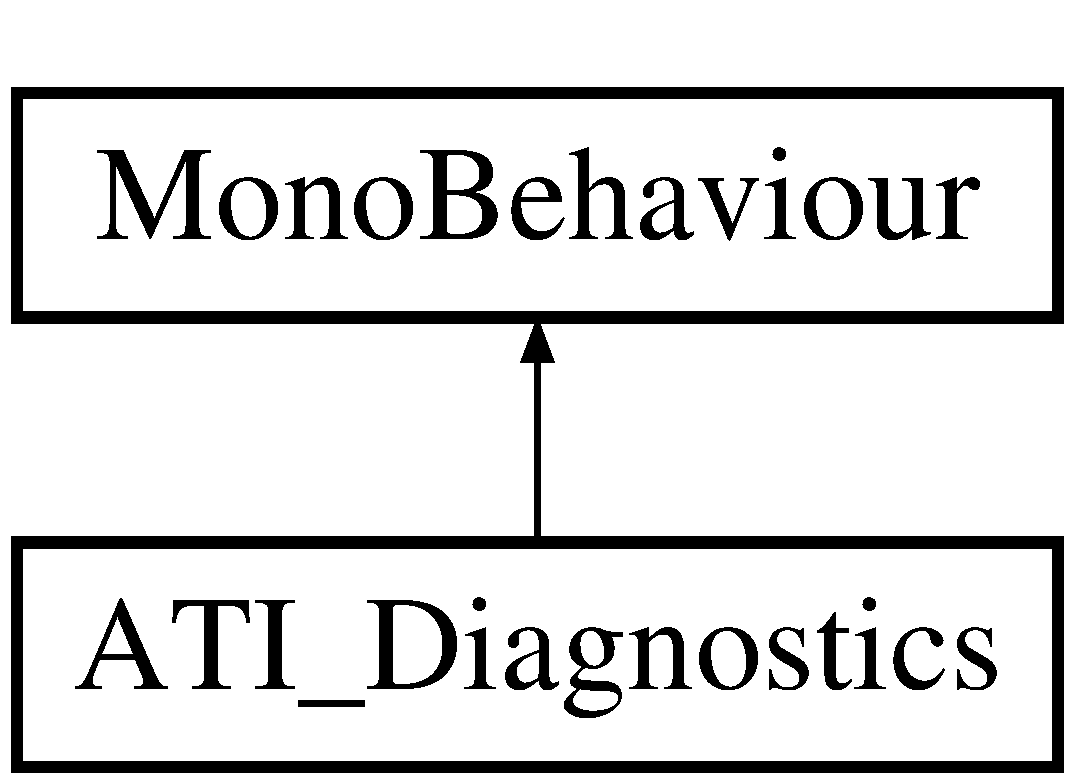
\includegraphics[height=2.000000cm]{group___audio_testing}
\end{center}
\end{figure}
\subsubsection*{Events}
\begin{DoxyCompactItemize}
\item 
Unity\+Event \hyperlink{group___audio_testing_a133561901c2aef535b2f3c098e55b959}{Set\+Input\+Time}
\begin{DoxyCompactList}\small\item\em The event that is invoked when the note event occurs. \end{DoxyCompactList}\item 
Unity\+Event \hyperlink{group___audio_testing_a6360e6098323b921b4a1b306914d06ef}{Set\+Output\+Time}
\begin{DoxyCompactList}\small\item\em The event that is invoked when the note output occurs. \end{DoxyCompactList}\end{DoxyCompactItemize}
\subsubsection*{Private Variables}
\begin{DoxyCompactItemize}
\item 
System.\+Date\+Time \hyperlink{group___audio_testing_a683f09700eab208b7368ebcb82bbd3be}{m\+Input\+Time}
\begin{DoxyCompactList}\small\item\em A Date\+Time object to keep track of the note\textquotesingle{}s beginning time. \end{DoxyCompactList}\item 
System.\+Date\+Time \hyperlink{group___audio_testing_a2e6f675a990948db789381f52071e1bf}{m\+Output\+Time}
\begin{DoxyCompactList}\small\item\em A Date\+Time object to keep track of when the note actually plays. \end{DoxyCompactList}\item 
Text \hyperlink{group___audio_testing_a8929a6a2ae14ec733b936a72cb0f44a6}{m\+Latency\+Text} = null
\begin{DoxyCompactList}\small\item\em The text object which displays latency. \end{DoxyCompactList}\end{DoxyCompactItemize}
\subsubsection*{Unity Functions}
\begin{DoxyCompactItemize}
\item 
void \hyperlink{group___audio_testing_a41cd250c9f5eea98dec6f32f49aa727f}{Awake} ()
\begin{DoxyCompactList}\small\item\em Called when the object is created. Gets the display text and sets up events. \end{DoxyCompactList}\item 
void \hyperlink{group___audio_testing_a4d131588b33317383ff7430b2917658e}{Update} ()
\begin{DoxyCompactList}\small\item\em Called every frame. Used to update text. \end{DoxyCompactList}\end{DoxyCompactItemize}
\subsubsection*{Event Handlers}
\begin{DoxyCompactItemize}
\item 
void \hyperlink{group___audio_testing_afcdfad4dc61b1f22a6efcef738897515}{Update\+Input\+Time} ()
\begin{DoxyCompactList}\small\item\em Update the input time. \end{DoxyCompactList}\item 
void \hyperlink{group___audio_testing_ac172cf129d078d8b0e979bc17d11c5a0}{Update\+Output\+Time} ()
\begin{DoxyCompactList}\small\item\em Updates the output time. \end{DoxyCompactList}\end{DoxyCompactItemize}


\paragraph{Member Function Documentation}
\mbox{\Hypertarget{group___audio_testing_a41cd250c9f5eea98dec6f32f49aa727f}\label{group___audio_testing_a41cd250c9f5eea98dec6f32f49aa727f}} 
\index{A\+T\+I\+\_\+\+Diagnostics@{A\+T\+I\+\_\+\+Diagnostics}!Awake@{Awake}}
\index{Awake@{Awake}!A\+T\+I\+\_\+\+Diagnostics@{A\+T\+I\+\_\+\+Diagnostics}}
\subparagraph{\texorpdfstring{Awake()}{Awake()}}
{\footnotesize\ttfamily void A\+T\+I\+\_\+\+Diagnostics.\+Awake (\begin{DoxyParamCaption}{ }\end{DoxyParamCaption})\hspace{0.3cm}{\ttfamily [private]}}



Called when the object is created. Gets the display text and sets up events. 



Definition at line 51 of file A\+T\+I\+\_\+\+Diagnostics.\+cs.



References m\+Input\+Time, m\+Output\+Time, Update\+Input\+Time(), and Update\+Output\+Time().


\begin{DoxyCode}
52     \{
53         \textcolor{comment}{// Get the text to display latency.}
54         \hyperlink{group___audio_testing_a8929a6a2ae14ec733b936a72cb0f44a6}{mLatencyText} = transform.GetChild( 0 ).GetComponent<Text>();
55         \hyperlink{group___audio_testing_a8929a6a2ae14ec733b936a72cb0f44a6}{mLatencyText}.text = \textcolor{stringliteral}{"Latency: N/A"};
56 
57         \textcolor{comment}{// Set up the input and output time.}
58         \hyperlink{group___audio_testing_a683f09700eab208b7368ebcb82bbd3be}{mInputTime} = \hyperlink{namespace_system}{System}.DateTime.Now;
59         \hyperlink{group___audio_testing_a2e6f675a990948db789381f52071e1bf}{mOutputTime} = \hyperlink{namespace_system}{System}.DateTime.Now;
60 
61         \textcolor{comment}{// Set up the events:}
62         \hyperlink{group___audio_testing_a133561901c2aef535b2f3c098e55b959}{SetInputTime} = \textcolor{keyword}{new} UnityEvent();
63         \hyperlink{group___audio_testing_a133561901c2aef535b2f3c098e55b959}{SetInputTime}.AddListener( \hyperlink{group___audio_testing_afcdfad4dc61b1f22a6efcef738897515}{UpdateInputTime} );
64         \hyperlink{group___audio_testing_a6360e6098323b921b4a1b306914d06ef}{SetOutputTime} = \textcolor{keyword}{new} UnityEvent();
65         \hyperlink{group___audio_testing_a6360e6098323b921b4a1b306914d06ef}{SetOutputTime}.AddListener( \hyperlink{group___audio_testing_ac172cf129d078d8b0e979bc17d11c5a0}{UpdateOutputTime} );
66     \}
\end{DoxyCode}
\mbox{\Hypertarget{group___audio_testing_a4d131588b33317383ff7430b2917658e}\label{group___audio_testing_a4d131588b33317383ff7430b2917658e}} 
\index{A\+T\+I\+\_\+\+Diagnostics@{A\+T\+I\+\_\+\+Diagnostics}!Update@{Update}}
\index{Update@{Update}!A\+T\+I\+\_\+\+Diagnostics@{A\+T\+I\+\_\+\+Diagnostics}}
\subparagraph{\texorpdfstring{Update()}{Update()}}
{\footnotesize\ttfamily void A\+T\+I\+\_\+\+Diagnostics.\+Update (\begin{DoxyParamCaption}{ }\end{DoxyParamCaption})\hspace{0.3cm}{\ttfamily [private]}}



Called every frame. Used to update text. 



Definition at line 71 of file A\+T\+I\+\_\+\+Diagnostics.\+cs.



References m\+Input\+Time, and m\+Output\+Time.


\begin{DoxyCode}
72     \{
73         \textcolor{comment}{// Update the display.}
74         \hyperlink{group___audio_testing_a8929a6a2ae14ec733b936a72cb0f44a6}{mLatencyText}.text = \textcolor{stringliteral}{"Latency: "} + ( \hyperlink{group___audio_testing_a2e6f675a990948db789381f52071e1bf}{mOutputTime} - 
      \hyperlink{group___audio_testing_a683f09700eab208b7368ebcb82bbd3be}{mInputTime} ).ToString();
75     \}
\end{DoxyCode}
\mbox{\Hypertarget{group___audio_testing_afcdfad4dc61b1f22a6efcef738897515}\label{group___audio_testing_afcdfad4dc61b1f22a6efcef738897515}} 
\index{A\+T\+I\+\_\+\+Diagnostics@{A\+T\+I\+\_\+\+Diagnostics}!Update\+Input\+Time@{Update\+Input\+Time}}
\index{Update\+Input\+Time@{Update\+Input\+Time}!A\+T\+I\+\_\+\+Diagnostics@{A\+T\+I\+\_\+\+Diagnostics}}
\subparagraph{\texorpdfstring{Update\+Input\+Time()}{UpdateInputTime()}}
{\footnotesize\ttfamily void A\+T\+I\+\_\+\+Diagnostics.\+Update\+Input\+Time (\begin{DoxyParamCaption}{ }\end{DoxyParamCaption})\hspace{0.3cm}{\ttfamily [private]}}



Update the input time. 



Definition at line 86 of file A\+T\+I\+\_\+\+Diagnostics.\+cs.



References m\+Input\+Time.



Referenced by Awake().


\begin{DoxyCode}
87     \{
88         \hyperlink{group___audio_testing_a683f09700eab208b7368ebcb82bbd3be}{mInputTime} = \hyperlink{namespace_system}{System}.DateTime.Now;
89     \}
\end{DoxyCode}
\mbox{\Hypertarget{group___audio_testing_ac172cf129d078d8b0e979bc17d11c5a0}\label{group___audio_testing_ac172cf129d078d8b0e979bc17d11c5a0}} 
\index{A\+T\+I\+\_\+\+Diagnostics@{A\+T\+I\+\_\+\+Diagnostics}!Update\+Output\+Time@{Update\+Output\+Time}}
\index{Update\+Output\+Time@{Update\+Output\+Time}!A\+T\+I\+\_\+\+Diagnostics@{A\+T\+I\+\_\+\+Diagnostics}}
\subparagraph{\texorpdfstring{Update\+Output\+Time()}{UpdateOutputTime()}}
{\footnotesize\ttfamily void A\+T\+I\+\_\+\+Diagnostics.\+Update\+Output\+Time (\begin{DoxyParamCaption}{ }\end{DoxyParamCaption})\hspace{0.3cm}{\ttfamily [private]}}



Updates the output time. 



Definition at line 94 of file A\+T\+I\+\_\+\+Diagnostics.\+cs.



References m\+Output\+Time.



Referenced by Awake().


\begin{DoxyCode}
95     \{
96         \textcolor{comment}{// Get the output time.}
97         \hyperlink{group___audio_testing_a2e6f675a990948db789381f52071e1bf}{mOutputTime} = \hyperlink{namespace_system}{System}.DateTime.Now;
98         GC.Collect();
99     \}
\end{DoxyCode}


\paragraph{Member Data Documentation}
\mbox{\Hypertarget{group___audio_testing_a683f09700eab208b7368ebcb82bbd3be}\label{group___audio_testing_a683f09700eab208b7368ebcb82bbd3be}} 
\index{A\+T\+I\+\_\+\+Diagnostics@{A\+T\+I\+\_\+\+Diagnostics}!m\+Input\+Time@{m\+Input\+Time}}
\index{m\+Input\+Time@{m\+Input\+Time}!A\+T\+I\+\_\+\+Diagnostics@{A\+T\+I\+\_\+\+Diagnostics}}
\subparagraph{\texorpdfstring{m\+Input\+Time}{mInputTime}}
{\footnotesize\ttfamily System.\+Date\+Time A\+T\+I\+\_\+\+Diagnostics.\+m\+Input\+Time\hspace{0.3cm}{\ttfamily [private]}}



A Date\+Time object to keep track of the note\textquotesingle{}s beginning time. 



Definition at line 38 of file A\+T\+I\+\_\+\+Diagnostics.\+cs.



Referenced by Awake(), Update(), and Update\+Input\+Time().

\mbox{\Hypertarget{group___audio_testing_a8929a6a2ae14ec733b936a72cb0f44a6}\label{group___audio_testing_a8929a6a2ae14ec733b936a72cb0f44a6}} 
\index{A\+T\+I\+\_\+\+Diagnostics@{A\+T\+I\+\_\+\+Diagnostics}!m\+Latency\+Text@{m\+Latency\+Text}}
\index{m\+Latency\+Text@{m\+Latency\+Text}!A\+T\+I\+\_\+\+Diagnostics@{A\+T\+I\+\_\+\+Diagnostics}}
\subparagraph{\texorpdfstring{m\+Latency\+Text}{mLatencyText}}
{\footnotesize\ttfamily Text A\+T\+I\+\_\+\+Diagnostics.\+m\+Latency\+Text = null\hspace{0.3cm}{\ttfamily [private]}}



The text object which displays latency. 



Definition at line 40 of file A\+T\+I\+\_\+\+Diagnostics.\+cs.

\mbox{\Hypertarget{group___audio_testing_a2e6f675a990948db789381f52071e1bf}\label{group___audio_testing_a2e6f675a990948db789381f52071e1bf}} 
\index{A\+T\+I\+\_\+\+Diagnostics@{A\+T\+I\+\_\+\+Diagnostics}!m\+Output\+Time@{m\+Output\+Time}}
\index{m\+Output\+Time@{m\+Output\+Time}!A\+T\+I\+\_\+\+Diagnostics@{A\+T\+I\+\_\+\+Diagnostics}}
\subparagraph{\texorpdfstring{m\+Output\+Time}{mOutputTime}}
{\footnotesize\ttfamily System.\+Date\+Time A\+T\+I\+\_\+\+Diagnostics.\+m\+Output\+Time\hspace{0.3cm}{\ttfamily [private]}}



A Date\+Time object to keep track of when the note actually plays. 



Definition at line 39 of file A\+T\+I\+\_\+\+Diagnostics.\+cs.



Referenced by Awake(), Update(), and Update\+Output\+Time().

\mbox{\Hypertarget{group___audio_testing_a133561901c2aef535b2f3c098e55b959}\label{group___audio_testing_a133561901c2aef535b2f3c098e55b959}} 
\index{A\+T\+I\+\_\+\+Diagnostics@{A\+T\+I\+\_\+\+Diagnostics}!Set\+Input\+Time@{Set\+Input\+Time}}
\index{Set\+Input\+Time@{Set\+Input\+Time}!A\+T\+I\+\_\+\+Diagnostics@{A\+T\+I\+\_\+\+Diagnostics}}
\subparagraph{\texorpdfstring{Set\+Input\+Time}{SetInputTime}}
{\footnotesize\ttfamily Unity\+Event A\+T\+I\+\_\+\+Diagnostics.\+Set\+Input\+Time}



The event that is invoked when the note event occurs. 



Definition at line 30 of file A\+T\+I\+\_\+\+Diagnostics.\+cs.



Referenced by Key\+Container.\+Handle\+Black\+Key\+Pressed(), Key\+Container.\+Handle\+White\+Key\+Pressed(), and Musical\+Typing\+Handler.\+On\+Musical\+Typing\+Event().

\mbox{\Hypertarget{group___audio_testing_a6360e6098323b921b4a1b306914d06ef}\label{group___audio_testing_a6360e6098323b921b4a1b306914d06ef}} 
\index{A\+T\+I\+\_\+\+Diagnostics@{A\+T\+I\+\_\+\+Diagnostics}!Set\+Output\+Time@{Set\+Output\+Time}}
\index{Set\+Output\+Time@{Set\+Output\+Time}!A\+T\+I\+\_\+\+Diagnostics@{A\+T\+I\+\_\+\+Diagnostics}}
\subparagraph{\texorpdfstring{Set\+Output\+Time}{SetOutputTime}}
{\footnotesize\ttfamily Unity\+Event A\+T\+I\+\_\+\+Diagnostics.\+Set\+Output\+Time}



The event that is invoked when the note output occurs. 



Definition at line 31 of file A\+T\+I\+\_\+\+Diagnostics.\+cs.



Referenced by Note\+Output\+Object.\+On\+Audio\+Filter\+Read().


\hypertarget{group___doc_a_t_i}{}\section{Audio Testing Interface}
\label{group___doc_a_t_i}\index{Audio Testing Interface@{Audio Testing Interface}}


Modules for the interface which is used to test the Audio.  


\subsection*{Modules}
\begin{DoxyCompactItemize}
\item 
\hyperlink{group___doc_a_t_i_buttons}{Buttons}
\begin{DoxyCompactList}\small\item\em Handler for buttons on the Audio Testing Interface. \end{DoxyCompactList}\end{DoxyCompactItemize}


\subsection{Detailed Description}
Modules for the interface which is used to test the Audio. 


\hypertarget{group___doc_black_key}{}\section{Black Key}
\label{group___doc_black_key}\index{Black Key@{Black Key}}


A script for handling the behavior of a black key on the keyboard.  


\subsection*{Modules}
\begin{DoxyCompactItemize}
\item 
\hyperlink{group___black_key_event_types}{Event Types}
\item 
\hyperlink{group___black_key_events}{Events}
\item 
\hyperlink{group___black_key_priv_var}{Private Variables}
\item 
\hyperlink{group___black_key_pub_func}{Public Functions}
\item 
\hyperlink{group___black_key_pub_var}{Public Variables}
\item 
\hyperlink{group___black_key_unity}{Unity Functions}
\end{DoxyCompactItemize}


\subsection{Detailed Description}
A script for handling the behavior of a black key on the keyboard. 

\hypertarget{group___doc_black_key_DocBlackKeyInfo}{}\subsection{Information}\label{group___doc_black_key_DocBlackKeyInfo}
This class defines the behavior for a Unity Game\+Object that represents a black key on the keyboard.\hypertarget{group___doc_black_key_DocBlackKeyEventTypes}{}\subsection{Event Types}\label{group___doc_black_key_DocBlackKeyEventTypes}
The types of events for the \hyperlink{group___doc_black_key}{black keys}. ~\newline
 \hyperlink{group___black_key_event_types}{More details}.\hypertarget{group___doc_black_key_DocBlackKeyEvents}{}\subsection{Events}\label{group___doc_black_key_DocBlackKeyEvents}
Events used by the \hyperlink{group___doc_black_key}{black keys} ~\newline
 \hyperlink{group___black_key_events}{More details}.\hypertarget{group___doc_black_key_DocBlackKeyPubVar}{}\subsection{Public Variables}\label{group___doc_black_key_DocBlackKeyPubVar}
Variables to set attributes of a \hyperlink{class_black_key}{Black\+Key} in the Unity Editor. ~\newline
 \hyperlink{group___black_key_pub_var}{More details}.\hypertarget{group___doc_black_key_DocBlackKeyPrivVar}{}\subsection{Private Variables}\label{group___doc_black_key_DocBlackKeyPrivVar}
Variables used internally by the \hyperlink{class_black_key}{Black\+Key} ~\newline
 \hyperlink{group___black_key_priv_var}{More details}.\hypertarget{group___doc_black_key_DocBlackKeyUnity}{}\subsection{Unity Functions}\label{group___doc_black_key_DocBlackKeyUnity}
Built-\/in Unity functions for creating and updating the \hyperlink{class_black_key}{Black\+Key}. ~\newline
 \hyperlink{group___black_key_unity}{More details}.\hypertarget{group___doc_black_key_DocBlackKeyPubFunc}{}\subsection{Private Functions}\label{group___doc_black_key_DocBlackKeyPubFunc}
Functions for other classes to configure the \hyperlink{class_black_key}{Black\+Key}. ~\newline
 \hyperlink{group___black_key_pub_func}{More details}.\hypertarget{group___doc_black_key_DocBlackKeyCode}{}\subsection{Code}\label{group___doc_black_key_DocBlackKeyCode}

\begin{DoxyCodeInclude}
1 \textcolor{keyword}{using} \hyperlink{namespace_system}{System}.Collections;
2 \textcolor{keyword}{using} \hyperlink{namespace_system}{System}.Collections.Generic;
3 \textcolor{keyword}{using} \hyperlink{namespace_unity_engine}{UnityEngine};
4 \textcolor{keyword}{using} \hyperlink{namespace_unity_engine}{UnityEngine}.Events;
5 \textcolor{comment}{}
6 \textcolor{comment}{/** }
7 \textcolor{comment}{ * @class BlackKey}
8 \textcolor{comment}{ * @brief A script for handling the behavior of a black key on the keyboard.}
9 \textcolor{comment}{ *  }
10 \textcolor{comment}{ * This class defines the behavior for a Unity GameObject that represents}
11 \textcolor{comment}{ * a black key on the keyboard.}
12 \textcolor{comment}{*/}
13 
14 \textcolor{keyword}{public} \textcolor{keyword}{class }\hyperlink{class_black_key}{BlackKey} : MonoBehaviour
15 \{
16     \textcolor{comment}{/*************************************************************************/}\textcolor{comment}{/** }
17 \textcolor{comment}{     * @\}}
18 \textcolor{comment}{     * @defgroup BlackKeyEventTypes Event Types}
19 \textcolor{comment}{     * @ingroup DocBlackKey}
20 \textcolor{comment}{     * The types of events for the @link DocBlackKey black keys@endlink.}
21 \textcolor{comment}{     * @\{}
22 \textcolor{comment}{    ****************************************************************************/}
23     \textcolor{keyword}{public} \textcolor{keyword}{class }BlackKeyPressedEvent : UnityEvent<BlackKey> \{ \} \textcolor{comment}{//!< Used for testing the container. Will
       probably need to change later.}
24 \textcolor{comment}{}    \textcolor{keyword}{public} \textcolor{keyword}{class }BlackKeyReleasedEvent : UnityEvent<BlackKey> \{ \} \textcolor{comment}{//!< Used for testing the container. Will
       probably need to change later.}
25 \textcolor{comment}{}
26     \textcolor{comment}{/*************************************************************************/}\textcolor{comment}{/** }
27 \textcolor{comment}{     * @\}}
28 \textcolor{comment}{     * @defgroup BlackKeyEvents Events}
29 \textcolor{comment}{     * @ingroup DocBlackKey}
30 \textcolor{comment}{     * Events used by the @link DocBlackKey black keys@endlink}
31 \textcolor{comment}{     * @\{}
32 \textcolor{comment}{    ****************************************************************************/}
33     \textcolor{keyword}{public} BlackKeyPressedEvent BlackKeyPressed = null; \textcolor{comment}{//!< Used for testing the container. Will probably
       need to change later.}
34 \textcolor{comment}{}    \textcolor{keyword}{public} BlackKeyReleasedEvent BlackKeyReleased = null; \textcolor{comment}{//!< Used for testing the container. Will
       probably need to change later.}
35 \textcolor{comment}{}
36     \textcolor{comment}{/*************************************************************************/}\textcolor{comment}{/** }
37 \textcolor{comment}{     * @\}}
38 \textcolor{comment}{     * @defgroup BlackKeyPubVar Public Variables}
39 \textcolor{comment}{     * @ingroup DocBlackKey}
40 \textcolor{comment}{     * Variables to set attributes of a BlackKey in the Unity Editor.}
41 \textcolor{comment}{     * @\{}
42 \textcolor{comment}{    ****************************************************************************/}
43     \textcolor{keyword}{public} \textcolor{keywordtype}{float} \hyperlink{group___black_key_pub_var_ga6fb983b09b3b6f80eab375fcb43010c1}{Velocity}; \textcolor{comment}{//!< The velocity of the key object.}
44 \textcolor{comment}{}    \textcolor{keyword}{public} \hyperlink{class_music}{Music}.\hyperlink{group___music_enums_ga508f69b199ea518f935486c990edac1d}{PITCH} \hyperlink{group___black_key_pub_var_gad233c456182c9cef7c01486484940439}{Pitch} = \hyperlink{class_music}{Music}.\hyperlink{group___music_enums_ga508f69b199ea518f935486c990edac1d}{PITCH}.CS4; \textcolor{comment}{//!< The pitch that this key
       represents.}
45 \textcolor{comment}{}
46     \textcolor{comment}{// I put a default value since it'll mess up the dynamic loading otherwise.}
47     \textcolor{keyword}{public} \textcolor{keywordtype}{string} Key = \textcolor{stringliteral}{"A"}; \textcolor{comment}{//!< The key that begins pressing the black key. }
48 \textcolor{comment}{}
49     \textcolor{comment}{/*************************************************************************/}\textcolor{comment}{/** }
50 \textcolor{comment}{     * @\}}
51 \textcolor{comment}{     * @defgroup BlackKeyPrivVar Private Variables}
52 \textcolor{comment}{     * @ingroup DocBlackKey}
53 \textcolor{comment}{     * Variables used internally by the BlackKey}
54 \textcolor{comment}{     * @\{}
55 \textcolor{comment}{     ****************************************************************************/}
56     \textcolor{keyword}{private} \textcolor{keywordtype}{bool} mKeyPressed = \textcolor{keyword}{false}; \textcolor{comment}{//!< Has the note started?}
57 \textcolor{comment}{}    \textcolor{keyword}{private} KeyCode \hyperlink{group___black_key_priv_var_ga2272fa345880793dcd89f7ca942f6685}{mKeyCode}; \textcolor{comment}{//!< The keycode to check for when testing physics.}
58 \textcolor{comment}{}    \textcolor{keyword}{private} \hyperlink{class_key_container}{KeyContainer} mContainer = null; \textcolor{comment}{//!< The parent @link DocKeyContain
       container@endlink.}
59 \textcolor{comment}{}    \textcolor{keyword}{private} Rigidbody \hyperlink{group___black_key_priv_var_ga5185c6ea66892bcbe9e83eb615f39566}{mRigidBody}; \textcolor{comment}{//!< The rigidbody representing the key.}
60 \textcolor{comment}{}
61     \textcolor{comment}{/*************************************************************************/}\textcolor{comment}{/** }
62 \textcolor{comment}{     * @\}}
63 \textcolor{comment}{     * @defgroup BlackKeyUnity Unity Functions}
64 \textcolor{comment}{     * @ingroup DocBlackKey}
65 \textcolor{comment}{     * Built-in Unity functions for creating and updating the BlackKey.}
66 \textcolor{comment}{     * @\{}
67 \textcolor{comment}{     ****************************************************************************/}
68 \textcolor{comment}{}
69 \textcolor{comment}{    /**}
70 \textcolor{comment}{     * @brief Called when object is initialized.}
71 \textcolor{comment}{     * }
72 \textcolor{comment}{     * Sets the key that is used to simulate pressing the object and gets the RigidBody}
73 \textcolor{comment}{     * and sets that it shouldn't use gravity.}
74 \textcolor{comment}{     */}
75     \textcolor{keywordtype}{void} \hyperlink{group___black_key_unity_ga6e05fcdf362e52d9a71b4f25ad840b5b}{Awake}()
76     \{
77         mKeyCode = (KeyCode)\hyperlink{namespace_system}{System}.Enum.Parse( typeof( KeyCode ), Key );
78         mRigidBody = GetComponent<Rigidbody>();
79         mRigidBody.useGravity = \textcolor{keyword}{false};
80         BlackKeyPressed = \textcolor{keyword}{new} BlackKeyPressedEvent();
81         BlackKeyReleased = \textcolor{keyword}{new} BlackKeyReleasedEvent();
82     \}
83 \textcolor{comment}{}
84 \textcolor{comment}{    /**}
85 \textcolor{comment}{     * @brief Called every frame. Used for loading the VirtualInstrumentManager.}
86 \textcolor{comment}{     * }
87 \textcolor{comment}{     * Checks if audio should be loaded/unloaded and handles the asynchronous scene}
88 \textcolor{comment}{     * operation that does so.}
89 \textcolor{comment}{     */}
90     \textcolor{keywordtype}{void} \hyperlink{group___black_key_unity_ga24ef6b8b614685c5591868b9b23197ed}{Update}()
91     \{
92     \}
93 \textcolor{comment}{}
94 \textcolor{comment}{    /**}
95 \textcolor{comment}{     * @brief Called every physics step. Used for applying force to the RigidBody.}
96 \textcolor{comment}{     * }
97 \textcolor{comment}{     * Checks if the appropriate key was pressed and applies a force if so.}
98 \textcolor{comment}{     * It also calls the functions that send input to the VirtualInstrumentManager if}
99 \textcolor{comment}{     * needed.}
100 \textcolor{comment}{     */}
101     \textcolor{keywordtype}{void} \hyperlink{group___black_key_unity_gad8926397bba69558f5440eac2c38aff8}{FixedUpdate}()
102     \{
103         \textcolor{comment}{//float move = Input.GetAxis ("Horizontal");}
104         Vector3 movement = \textcolor{keyword}{new} Vector3( 0, -1f, 0 );
105         \textcolor{keywordflow}{if}( Input.GetKey( mKeyCode ) )
106         \{
107             \textcolor{comment}{//Debug.Log( Key );}
108             mRigidBody.AddForce( movement );
109 
110             \textcolor{comment}{// Let others know that this key was pressed.}
111             \textcolor{keywordflow}{if}( !mKeyPressed )
112             \{
113                 Debug.Log( \textcolor{stringliteral}{"Key representing "} + \hyperlink{class_music}{Music}.\hyperlink{group___music_stat_func_ga85a22c905d56d4c5f4e62159bfecee8c}{NoteToString}( 
      \hyperlink{group___black_key_pub_var_gad233c456182c9cef7c01486484940439}{Pitch} ) + \textcolor{stringliteral}{" was pressed."} );
114                 mKeyPressed = \textcolor{keyword}{true};
115                 BlackKeyPressed.Invoke( \textcolor{keyword}{this} );
116             \}
117 
118         \}
119         \textcolor{keywordflow}{else}
120         \{
121             \textcolor{comment}{// If the key is released, then let others know.}
122             \textcolor{keywordflow}{if}( mKeyPressed )
123             \{
124                 Debug.Log( \textcolor{stringliteral}{"Key representing "} + \hyperlink{class_music}{Music}.\hyperlink{group___music_stat_func_ga85a22c905d56d4c5f4e62159bfecee8c}{NoteToString}( 
      \hyperlink{group___black_key_pub_var_gad233c456182c9cef7c01486484940439}{Pitch} ) + \textcolor{stringliteral}{" was released."} );
125                 mKeyPressed = \textcolor{keyword}{false};
126                 BlackKeyReleased.Invoke( \textcolor{keyword}{this} );
127             \}
128         \}
129     \}
130 
131     \textcolor{comment}{/*************************************************************************/}\textcolor{comment}{/** }
132 \textcolor{comment}{     * @\}}
133 \textcolor{comment}{     * @defgroup BlackKeyPubFunc Public Functions}
134 \textcolor{comment}{     * @ingroup DocBlackKey}
135 \textcolor{comment}{     * Functions for other classes to configure the BlackKey.}
136 \textcolor{comment}{     * @\{}
137 \textcolor{comment}{    *****************************************************************************/}
138 \textcolor{comment}{}
139 \textcolor{comment}{    /**}
140 \textcolor{comment}{     * @brief Sets the @link DocKeyContain parent container@endlink.}
141 \textcolor{comment}{     * @param[in] aContainer The parent container.}
142 \textcolor{comment}{    */}
143     \textcolor{keyword}{public} \textcolor{keywordtype}{void} \hyperlink{group___black_key_pub_func_ga49d807a46e36ba19211be329db1cbd2e}{SetParentContainer}( \hyperlink{class_key_container}{KeyContainer} aContainer )
144     \{
145         mContainer = aContainer;
146     \}
147 \textcolor{comment}{}
148 \textcolor{comment}{    /** @\} */}
149 \}
150 
151 
\end{DoxyCodeInclude}
 
\hypertarget{group___doc_a_t_i_buttons}{}\section{Buttons}
\label{group___doc_a_t_i_buttons}\index{Buttons@{Buttons}}


Handler for buttons on the Audio Testing Interface.  


\subsection*{Modules}
\begin{DoxyCompactItemize}
\item 
\hyperlink{group___a_t_i_buttons_priv_var}{Private Variables}
\item 
\hyperlink{group___a_t_i_buttons_unity}{Unity Functions}
\end{DoxyCompactItemize}


\subsection{Detailed Description}
Handler for buttons on the Audio Testing Interface. 

\hypertarget{group___doc_a_t_i_buttons_DocATIButtonsPrivVar}{}\subsection{Private Variables}\label{group___doc_a_t_i_buttons_DocATIButtonsPrivVar}
These are references to the buttons. ~\newline
 \hyperlink{group___a_t_i_buttons_priv_var}{More details}.\hypertarget{group___doc_a_t_i_buttons_DocATIButtonsUnity}{}\subsection{Unity Functions}\label{group___doc_a_t_i_buttons_DocATIButtonsUnity}
These are functions automatically called by Unity. ~\newline
 \hyperlink{group___a_t_i_buttons_unity}{More details}.\hypertarget{group___doc_a_t_i_buttons_DocATIButtonsHandlers}{}\subsection{Event Handlers}\label{group___doc_a_t_i_buttons_DocATIButtonsHandlers}
These are functions used by \hyperlink{class_a_t_i___buttons}{A\+T\+I\+\_\+\+Buttons} to handle the buttons being clicked. ~\newline
 \hyperlink{group___a_t_i_buttons_handlers}{More details}.\hypertarget{group___doc_a_t_i_buttons_DocATIButtonsCode}{}\subsection{Code}\label{group___doc_a_t_i_buttons_DocATIButtonsCode}

\begin{DoxyCodeInclude}
1 \textcolor{keyword}{using} \hyperlink{namespace_system}{System}.Collections;
2 \textcolor{keyword}{using} \hyperlink{namespace_system}{System}.Collections.Generic;
3 \textcolor{keyword}{using} \hyperlink{namespace_unity_engine}{UnityEngine};
4 \textcolor{keyword}{using} \hyperlink{namespace_unity_engine}{UnityEngine}.Assertions;
5 \textcolor{keyword}{using} \hyperlink{namespace_unity_engine}{UnityEngine}.SceneManagement;
6 \textcolor{keyword}{using} \hyperlink{namespace_unity_engine}{UnityEngine}.UI;
7 \textcolor{comment}{}
8 \textcolor{comment}{/**}
9 \textcolor{comment}{ * @class ATI\_Buttons}
10 \textcolor{comment}{ * @brief Handler for buttons on the Audio Testing Interface.}
11 \textcolor{comment}{*/}
12 \textcolor{keyword}{public} \textcolor{keyword}{class }\hyperlink{class_a_t_i___buttons}{ATI\_Buttons} : MonoBehaviour
13 \{
14 
15     \textcolor{comment}{/*************************************************************************/}\textcolor{comment}{/** }
16 \textcolor{comment}{    * @defgroup ATIButtonsPrivVar Private Variables}
17 \textcolor{comment}{    * @ingroup DocATIButtons}
18 \textcolor{comment}{    * These are references to the buttons.}
19 \textcolor{comment}{    * @\{}
20 \textcolor{comment}{    ****************************************************************************/}
21     \textcolor{keyword}{private} Button      mLoadSongCreationButton = null; \textcolor{comment}{//!< The button that loads the song creation
       interface when clicked.}
22 \textcolor{comment}{}    \textcolor{keyword}{private} Button      mLoadKeyboardSceneButton = null; \textcolor{comment}{//!< The button that loads the keyboard scene.}
23 \textcolor{comment}{}
24     \textcolor{comment}{/*************************************************************************/}\textcolor{comment}{/** }
25 \textcolor{comment}{    * @\}}
26 \textcolor{comment}{    * @defgroup ATIButtonsUnity Unity Functions}
27 \textcolor{comment}{    * @ingroup DocATIButtons}
28 \textcolor{comment}{    * These are functions automatically called by Unity.}
29 \textcolor{comment}{    * @\{}
30 \textcolor{comment}{    ****************************************************************************/}
31 \textcolor{comment}{}
32 \textcolor{comment}{    /**}
33 \textcolor{comment}{     * @brief Gets references to the buttons and adds their listeners. Called when the object is created.}
34 \textcolor{comment}{    */}
35     \textcolor{keywordtype}{void} \hyperlink{group___a_t_i_buttons_unity_gaa24ae34a40539dab6595d1713fc77560}{Awake}()
36     \{
37         \textcolor{comment}{// Get the buttons.}
38         mLoadSongCreationButton = transform.GetChild( 0 ).GetComponent<Button>();
39         Assert.IsNotNull( mLoadSongCreationButton, \textcolor{stringliteral}{"Could not find the button to load the Song Creation
       Interface!"} );
40 
41         mLoadKeyboardSceneButton = transform.GetChild( 1 ).GetComponent<Button>();
42         Assert.IsNotNull( mLoadKeyboardSceneButton, \textcolor{stringliteral}{"Could not find the button to load the Keyboard scene!"}
       );
43 
44         \textcolor{comment}{// Add the listeners.}
45         mLoadSongCreationButton.onClick.AddListener( 
      \hyperlink{group___a_t_i_buttons_unity_ga6f6e66c53a80c3bcd9b7e7238a3b82fd}{OnLoadSongCreationButtonClicked} );
46         mLoadKeyboardSceneButton.onClick.AddListener( 
      \hyperlink{group___a_t_i_buttons_unity_ga1b9e9b75184e9e26309cc14bda37ad8a}{OnLoadKeyboardSceneButtonClicked} );
47     \}
48 
49     \textcolor{comment}{/*************************************************************************/}\textcolor{comment}{/** }
50 \textcolor{comment}{    * @\{}
51 \textcolor{comment}{    * @defgroup ATIButtonsHandlers Event Handlers}
52 \textcolor{comment}{    * @ingroup DocATIButtons}
53 \textcolor{comment}{    * These are functions used by ATI\_Buttons to handle the buttons being clicked.}
54 \textcolor{comment}{    * @\}}
55 \textcolor{comment}{    ****************************************************************************/}
56 \textcolor{comment}{}
57 \textcolor{comment}{    /**}
58 \textcolor{comment}{    * @brief Loads the song creation interface scene.}
59 \textcolor{comment}{    */}
60     \textcolor{keyword}{private} \textcolor{keywordtype}{void} \hyperlink{group___a_t_i_buttons_unity_ga1b9e9b75184e9e26309cc14bda37ad8a}{OnLoadKeyboardSceneButtonClicked}()
61     \{
62         SceneManager.LoadScene( \textcolor{stringliteral}{"KeyboardScene"}, LoadSceneMode.Single );
63     \}
64 \textcolor{comment}{}
65 \textcolor{comment}{    /**}
66 \textcolor{comment}{     * @brief Loads the song creation interface scene.}
67 \textcolor{comment}{    */}
68     \textcolor{keyword}{private} \textcolor{keywordtype}{void} \hyperlink{group___a_t_i_buttons_unity_ga6f6e66c53a80c3bcd9b7e7238a3b82fd}{OnLoadSongCreationButtonClicked}()
69     \{
70         SceneManager.LoadScene( \textcolor{stringliteral}{"SongCreationInterfaceScene"}, LoadSceneMode.Additive );
71     \}\textcolor{comment}{}
72 \textcolor{comment}{    /** @\} */}
73 \}
\end{DoxyCodeInclude}
 
\hypertarget{group___music_constants}{}\section{Constants}
\label{group___music_constants}\index{Constants@{Constants}}
\subsection*{Variables}
\begin{DoxyCompactItemize}
\item 
static string \mbox{[}$\,$\mbox{]} \hyperlink{group___music_constants_ga1381281d147886a2cf3584ab0c7a67d6}{Music.\+D\+R\+U\+M\+\_\+\+S\+T\+R\+I\+NG}
\begin{DoxyCompactList}\small\item\em An array of strings that represent the name of each type of drum. \end{DoxyCompactList}\item 
static string \mbox{[}$\,$\mbox{]} \hyperlink{group___music_constants_ga0f6eb5ac330d374c6b5021a0ba11c2bc}{Music.\+P\+I\+T\+C\+H\+\_\+\+S\+T\+R\+I\+NG} = \{ \char`\"{}C\char`\"{}, \char`\"{}CS\char`\"{}, \char`\"{}D\char`\"{}, \char`\"{}DS\char`\"{}, \char`\"{}E\char`\"{}, \char`\"{}F\char`\"{}, \char`\"{}FS\char`\"{}, \char`\"{}G\char`\"{}, \char`\"{}GS\char`\"{}, \char`\"{}A\char`\"{}, \char`\"{}AS\char`\"{}, \char`\"{}B\char`\"{} \}
\begin{DoxyCompactList}\small\item\em An array of strings that represent each pitch in an octave. \end{DoxyCompactList}\item 
static short \hyperlink{group___music_constants_gab346f7d8791bf021799da7786cde44c1}{Music.\+N\+U\+M\+\_\+\+N\+O\+T\+E\+S\+\_\+\+I\+N\+\_\+\+O\+C\+T\+A\+VE} = 12
\begin{DoxyCompactList}\small\item\em The number of notes in an octave. \end{DoxyCompactList}\item 
static int \hyperlink{group___music_constants_gaaf07da909a12e9fec0e43b70864f27b7}{Music.\+M\+A\+X\+\_\+\+S\+U\+P\+P\+O\+R\+T\+E\+D\+\_\+\+N\+O\+T\+ES} = 120
\begin{DoxyCompactList}\small\item\em The maximum number of pitches that a \hyperlink{class_virtual_instrument}{Virtual\+Instrument} could support. \end{DoxyCompactList}\item 
static int \hyperlink{group___music_constants_gabce1a1ac5b9b6355af6bd7fb3868467a}{Music.\+M\+A\+X\+\_\+\+S\+U\+P\+P\+O\+R\+T\+E\+D\+\_\+\+D\+R\+U\+MS} = 18
\begin{DoxyCompactList}\small\item\em The maximum number of drums that a \hyperlink{class_drum_kit}{Drum\+Kit} could support. \end{DoxyCompactList}\end{DoxyCompactItemize}


\subsection{Detailed Description}
These are constants used in the \hyperlink{group___music_stat_func}{static functions below}. 

\subsection{Variable Documentation}
\mbox{\Hypertarget{group___music_constants_ga1381281d147886a2cf3584ab0c7a67d6}\label{group___music_constants_ga1381281d147886a2cf3584ab0c7a67d6}} 
\index{Constants@{Constants}!D\+R\+U\+M\+\_\+\+S\+T\+R\+I\+NG@{D\+R\+U\+M\+\_\+\+S\+T\+R\+I\+NG}}
\index{D\+R\+U\+M\+\_\+\+S\+T\+R\+I\+NG@{D\+R\+U\+M\+\_\+\+S\+T\+R\+I\+NG}!Constants@{Constants}}
\subsubsection{\texorpdfstring{D\+R\+U\+M\+\_\+\+S\+T\+R\+I\+NG}{DRUM\_STRING}}
{\footnotesize\ttfamily string \mbox{[}$\,$\mbox{]} Music.\+D\+R\+U\+M\+\_\+\+S\+T\+R\+I\+NG\hspace{0.3cm}{\ttfamily [static]}}

{\bfseries Initial value\+:}
\begin{DoxyCode}
=
        \{ \textcolor{stringliteral}{"KICK\_1"}, \textcolor{stringliteral}{"KICK\_2"}, \textcolor{stringliteral}{"SNARE\_1"}, \textcolor{stringliteral}{"SNARE\_RIM"}, \textcolor{stringliteral}{"SNARE\_2"}, \textcolor{stringliteral}{"LOWTOM\_1"},
        \textcolor{stringliteral}{"HIHAT\_C"}, \textcolor{stringliteral}{"LOWTOM\_2"}, \textcolor{stringliteral}{"HIHAT\_P"}, \textcolor{stringliteral}{"MIDTOM\_1"}, \textcolor{stringliteral}{"HIHAT\_O"}, \textcolor{stringliteral}{"MIDTOM\_2"},
        \textcolor{stringliteral}{"HIGHTOM\_1"}, \textcolor{stringliteral}{"CRASH\_1"}, \textcolor{stringliteral}{"HIGHTOM\_2"}, \textcolor{stringliteral}{"RIDE"}, \textcolor{stringliteral}{"CRASH\_2"}, \textcolor{stringliteral}{"RIDE\_BELL"} \}
\end{DoxyCode}


An array of strings that represent the name of each type of drum. 



Definition at line 27 of file Music.\+cs.

\mbox{\Hypertarget{group___music_constants_gabce1a1ac5b9b6355af6bd7fb3868467a}\label{group___music_constants_gabce1a1ac5b9b6355af6bd7fb3868467a}} 
\index{Constants@{Constants}!M\+A\+X\+\_\+\+S\+U\+P\+P\+O\+R\+T\+E\+D\+\_\+\+D\+R\+U\+MS@{M\+A\+X\+\_\+\+S\+U\+P\+P\+O\+R\+T\+E\+D\+\_\+\+D\+R\+U\+MS}}
\index{M\+A\+X\+\_\+\+S\+U\+P\+P\+O\+R\+T\+E\+D\+\_\+\+D\+R\+U\+MS@{M\+A\+X\+\_\+\+S\+U\+P\+P\+O\+R\+T\+E\+D\+\_\+\+D\+R\+U\+MS}!Constants@{Constants}}
\subsubsection{\texorpdfstring{M\+A\+X\+\_\+\+S\+U\+P\+P\+O\+R\+T\+E\+D\+\_\+\+D\+R\+U\+MS}{MAX\_SUPPORTED\_DRUMS}}
{\footnotesize\ttfamily int Music.\+M\+A\+X\+\_\+\+S\+U\+P\+P\+O\+R\+T\+E\+D\+\_\+\+D\+R\+U\+MS = 18\hspace{0.3cm}{\ttfamily [static]}}



The maximum number of drums that a \hyperlink{class_drum_kit}{Drum\+Kit} could support. 



Definition at line 34 of file Music.\+cs.



Referenced by Drum\+Kit.\+Initialize\+Built\+In\+Dynamics(), Virtual\+Instrument.\+Load\+Audio\+Clips(), Virtual\+Instrument.\+Normalize\+Audio\+Clips(), and S\+C\+\_\+\+Pitch\+Selection\+Container.\+Set\+Up\+As\+Drum\+Selector().

\mbox{\Hypertarget{group___music_constants_gaaf07da909a12e9fec0e43b70864f27b7}\label{group___music_constants_gaaf07da909a12e9fec0e43b70864f27b7}} 
\index{Constants@{Constants}!M\+A\+X\+\_\+\+S\+U\+P\+P\+O\+R\+T\+E\+D\+\_\+\+N\+O\+T\+ES@{M\+A\+X\+\_\+\+S\+U\+P\+P\+O\+R\+T\+E\+D\+\_\+\+N\+O\+T\+ES}}
\index{M\+A\+X\+\_\+\+S\+U\+P\+P\+O\+R\+T\+E\+D\+\_\+\+N\+O\+T\+ES@{M\+A\+X\+\_\+\+S\+U\+P\+P\+O\+R\+T\+E\+D\+\_\+\+N\+O\+T\+ES}!Constants@{Constants}}
\subsubsection{\texorpdfstring{M\+A\+X\+\_\+\+S\+U\+P\+P\+O\+R\+T\+E\+D\+\_\+\+N\+O\+T\+ES}{MAX\_SUPPORTED\_NOTES}}
{\footnotesize\ttfamily int Music.\+M\+A\+X\+\_\+\+S\+U\+P\+P\+O\+R\+T\+E\+D\+\_\+\+N\+O\+T\+ES = 120\hspace{0.3cm}{\ttfamily [static]}}



The maximum number of pitches that a \hyperlink{class_virtual_instrument}{Virtual\+Instrument} could support. 



Definition at line 33 of file Music.\+cs.



Referenced by Marimba.\+Initialize\+Built\+In\+Dynamics(), Piano.\+Initialize\+Built\+In\+Dynamics(), Virtual\+Instrument.\+Load\+Audio\+Clips(), Virtual\+Instrument.\+Normalize\+Audio\+Clips(), and S\+C\+\_\+\+Pitch\+Selection\+Container.\+Set\+Up\+As\+Pitch\+Selector().

\mbox{\Hypertarget{group___music_constants_gab346f7d8791bf021799da7786cde44c1}\label{group___music_constants_gab346f7d8791bf021799da7786cde44c1}} 
\index{Constants@{Constants}!N\+U\+M\+\_\+\+N\+O\+T\+E\+S\+\_\+\+I\+N\+\_\+\+O\+C\+T\+A\+VE@{N\+U\+M\+\_\+\+N\+O\+T\+E\+S\+\_\+\+I\+N\+\_\+\+O\+C\+T\+A\+VE}}
\index{N\+U\+M\+\_\+\+N\+O\+T\+E\+S\+\_\+\+I\+N\+\_\+\+O\+C\+T\+A\+VE@{N\+U\+M\+\_\+\+N\+O\+T\+E\+S\+\_\+\+I\+N\+\_\+\+O\+C\+T\+A\+VE}!Constants@{Constants}}
\subsubsection{\texorpdfstring{N\+U\+M\+\_\+\+N\+O\+T\+E\+S\+\_\+\+I\+N\+\_\+\+O\+C\+T\+A\+VE}{NUM\_NOTES\_IN\_OCTAVE}}
{\footnotesize\ttfamily short Music.\+N\+U\+M\+\_\+\+N\+O\+T\+E\+S\+\_\+\+I\+N\+\_\+\+O\+C\+T\+A\+VE = 12\hspace{0.3cm}{\ttfamily [static]}}



The number of notes in an octave. 



Definition at line 32 of file Music.\+cs.

\mbox{\Hypertarget{group___music_constants_ga0f6eb5ac330d374c6b5021a0ba11c2bc}\label{group___music_constants_ga0f6eb5ac330d374c6b5021a0ba11c2bc}} 
\index{Constants@{Constants}!P\+I\+T\+C\+H\+\_\+\+S\+T\+R\+I\+NG@{P\+I\+T\+C\+H\+\_\+\+S\+T\+R\+I\+NG}}
\index{P\+I\+T\+C\+H\+\_\+\+S\+T\+R\+I\+NG@{P\+I\+T\+C\+H\+\_\+\+S\+T\+R\+I\+NG}!Constants@{Constants}}
\subsubsection{\texorpdfstring{P\+I\+T\+C\+H\+\_\+\+S\+T\+R\+I\+NG}{PITCH\_STRING}}
{\footnotesize\ttfamily string \mbox{[}$\,$\mbox{]} Music.\+P\+I\+T\+C\+H\+\_\+\+S\+T\+R\+I\+NG = \{ \char`\"{}C\char`\"{}, \char`\"{}CS\char`\"{}, \char`\"{}D\char`\"{}, \char`\"{}DS\char`\"{}, \char`\"{}E\char`\"{}, \char`\"{}F\char`\"{}, \char`\"{}FS\char`\"{}, \char`\"{}G\char`\"{}, \char`\"{}GS\char`\"{}, \char`\"{}A\char`\"{}, \char`\"{}AS\char`\"{}, \char`\"{}B\char`\"{} \}\hspace{0.3cm}{\ttfamily [static]}}



An array of strings that represent each pitch in an octave. 



Definition at line 31 of file Music.\+cs.


\hypertarget{group___s_c___n_d_c_const}{}\section{Constants}
\label{group___s_c___n_d_c_const}\index{Constants@{Constants}}
\subsection*{Variables}
\begin{DoxyCompactItemize}
\item 
const string \hyperlink{group___s_c___n_d_c_const_gabc95cd739b62996e8a19f0e9417e5f8e}{S\+C\+\_\+\+Note\+Display\+Container.\+M\+E\+A\+S\+U\+R\+E\+\_\+\+P\+A\+N\+E\+L\+\_\+\+P\+R\+E\+F\+A\+B\+\_\+\+P\+A\+TH} = \char`\"{}Audio/Prefabs/Song\+Creation/Measure\+Panel\+Prefab\char`\"{}
\begin{DoxyCompactList}\small\item\em The path to load the prefab for the \hyperlink{group___doc_s_c___m_d_p}{measure display panel objects}. \end{DoxyCompactList}\end{DoxyCompactItemize}


\subsection{Detailed Description}
Constants used by the \hyperlink{class_s_c___note_display_container}{S\+C\+\_\+\+Note\+Display\+Container}. 

\subsection{Variable Documentation}
\mbox{\Hypertarget{group___s_c___n_d_c_const_gabc95cd739b62996e8a19f0e9417e5f8e}\label{group___s_c___n_d_c_const_gabc95cd739b62996e8a19f0e9417e5f8e}} 
\index{Constants@{Constants}!M\+E\+A\+S\+U\+R\+E\+\_\+\+P\+A\+N\+E\+L\+\_\+\+P\+R\+E\+F\+A\+B\+\_\+\+P\+A\+TH@{M\+E\+A\+S\+U\+R\+E\+\_\+\+P\+A\+N\+E\+L\+\_\+\+P\+R\+E\+F\+A\+B\+\_\+\+P\+A\+TH}}
\index{M\+E\+A\+S\+U\+R\+E\+\_\+\+P\+A\+N\+E\+L\+\_\+\+P\+R\+E\+F\+A\+B\+\_\+\+P\+A\+TH@{M\+E\+A\+S\+U\+R\+E\+\_\+\+P\+A\+N\+E\+L\+\_\+\+P\+R\+E\+F\+A\+B\+\_\+\+P\+A\+TH}!Constants@{Constants}}
\subsubsection{\texorpdfstring{M\+E\+A\+S\+U\+R\+E\+\_\+\+P\+A\+N\+E\+L\+\_\+\+P\+R\+E\+F\+A\+B\+\_\+\+P\+A\+TH}{MEASURE\_PANEL\_PREFAB\_PATH}}
{\footnotesize\ttfamily const string S\+C\+\_\+\+Note\+Display\+Container.\+M\+E\+A\+S\+U\+R\+E\+\_\+\+P\+A\+N\+E\+L\+\_\+\+P\+R\+E\+F\+A\+B\+\_\+\+P\+A\+TH = \char`\"{}Audio/Prefabs/Song\+Creation/Measure\+Panel\+Prefab\char`\"{}\hspace{0.3cm}{\ttfamily [private]}}



The path to load the prefab for the \hyperlink{group___doc_s_c___m_d_p}{measure display panel objects}. 



Definition at line 21 of file S\+C\+\_\+\+Note\+Display\+Container.\+cs.


\hypertarget{group___s_c_m_const}{}\section{Constants}
\label{group___s_c_m_const}\index{Constants@{Constants}}
\subsection*{Variables}
\begin{DoxyCompactItemize}
\item 
string \hyperlink{group___s_c_m_const_ga821945ef78c5b9411d7861b42407591e}{Song\+Creation\+Manager.\+L\+O\+A\+D\+\_\+\+S\+O\+N\+G\+\_\+\+D\+I\+A\+L\+O\+G\+\_\+\+P\+A\+TH} = \char`\"{}Audio/Prefabs/Song\+Creation/Load\+Song\+Dialog\+Prefab\char`\"{}
\begin{DoxyCompactList}\small\item\em The path to load the \hyperlink{group___doc_s_c___l_s_d}{Load Song Dialog}\textquotesingle{}s prefab. \end{DoxyCompactList}\end{DoxyCompactItemize}


\subsection{Detailed Description}
These are paths to the prefabs that are used in the \hyperlink{group___doc_s_c}{Song Creation Interface}. 

\subsection{Variable Documentation}
\mbox{\Hypertarget{group___s_c_m_const_ga821945ef78c5b9411d7861b42407591e}\label{group___s_c_m_const_ga821945ef78c5b9411d7861b42407591e}} 
\index{Constants@{Constants}!L\+O\+A\+D\+\_\+\+S\+O\+N\+G\+\_\+\+D\+I\+A\+L\+O\+G\+\_\+\+P\+A\+TH@{L\+O\+A\+D\+\_\+\+S\+O\+N\+G\+\_\+\+D\+I\+A\+L\+O\+G\+\_\+\+P\+A\+TH}}
\index{L\+O\+A\+D\+\_\+\+S\+O\+N\+G\+\_\+\+D\+I\+A\+L\+O\+G\+\_\+\+P\+A\+TH@{L\+O\+A\+D\+\_\+\+S\+O\+N\+G\+\_\+\+D\+I\+A\+L\+O\+G\+\_\+\+P\+A\+TH}!Constants@{Constants}}
\subsubsection{\texorpdfstring{L\+O\+A\+D\+\_\+\+S\+O\+N\+G\+\_\+\+D\+I\+A\+L\+O\+G\+\_\+\+P\+A\+TH}{LOAD\_SONG\_DIALOG\_PATH}}
{\footnotesize\ttfamily string Song\+Creation\+Manager.\+L\+O\+A\+D\+\_\+\+S\+O\+N\+G\+\_\+\+D\+I\+A\+L\+O\+G\+\_\+\+P\+A\+TH = \char`\"{}Audio/Prefabs/Song\+Creation/Load\+Song\+Dialog\+Prefab\char`\"{}\hspace{0.3cm}{\ttfamily [private]}}



The path to load the \hyperlink{group___doc_s_c___l_s_d}{Load Song Dialog}\textquotesingle{}s prefab. 



Definition at line 27 of file Song\+Creation\+Manager.\+cs.


\hypertarget{group___v_i_base_const}{}\section{Constants}
\label{group___v_i_base_const}\index{Constants@{Constants}}
\subsection*{Modules}
\begin{DoxyCompactItemize}
\item 
\hyperlink{group___v_i_base_construct}{Constructors}
\item 
\hyperlink{group___v_i_base_priv_func}{Private Functions}
\item 
\hyperlink{group___v_i_base_pro_func}{Protected Functions}
\item 
\hyperlink{group___v_i_base_pro_var}{Protected Variables}
\item 
\hyperlink{group___v_i_base_pub_func}{Public Functions}
\item 
\hyperlink{group___v_i_base_virt_func}{Pure Virtual Functions}
\end{DoxyCompactItemize}
\subsection*{Variables}
\begin{DoxyCompactItemize}
\item 
static float \hyperlink{group___v_i_base_const_ga69a037919b64e1e3e0f2b949b2b6af2c}{Virtual\+Instrument.\+S\+A\+M\+P\+L\+E\+\_\+\+I\+N\+T\+E\+R\+V\+AL} = 1.\+1337e-\/5f
\begin{DoxyCompactList}\small\item\em The number of seconds between waveform samples. \end{DoxyCompactList}\item 
const float \hyperlink{group___v_i_base_const_gaf060c000443f92784bd8db8d866d8b2a}{Virtual\+Instrument.\+N\+O\+R\+M\+A\+L\+I\+Z\+E\+D\+\_\+\+P\+E\+AK} = -\/.\+1f
\begin{DoxyCompactList}\small\item\em The peak of the waveform after it\textquotesingle{}s normalized. \end{DoxyCompactList}\end{DoxyCompactItemize}


\subsection{Detailed Description}
Constants used in order to set attributes of the \hyperlink{group___v_i}{Virtual Instrument}. 

\subsection{Variable Documentation}
\mbox{\Hypertarget{group___v_i_base_const_gaf060c000443f92784bd8db8d866d8b2a}\label{group___v_i_base_const_gaf060c000443f92784bd8db8d866d8b2a}} 
\index{Constants@{Constants}!N\+O\+R\+M\+A\+L\+I\+Z\+E\+D\+\_\+\+P\+E\+AK@{N\+O\+R\+M\+A\+L\+I\+Z\+E\+D\+\_\+\+P\+E\+AK}}
\index{N\+O\+R\+M\+A\+L\+I\+Z\+E\+D\+\_\+\+P\+E\+AK@{N\+O\+R\+M\+A\+L\+I\+Z\+E\+D\+\_\+\+P\+E\+AK}!Constants@{Constants}}
\subsubsection{\texorpdfstring{N\+O\+R\+M\+A\+L\+I\+Z\+E\+D\+\_\+\+P\+E\+AK}{NORMALIZED\_PEAK}}
{\footnotesize\ttfamily const float Virtual\+Instrument.\+N\+O\+R\+M\+A\+L\+I\+Z\+E\+D\+\_\+\+P\+E\+AK = -\/.\+1f\hspace{0.3cm}{\ttfamily [private]}}



The peak of the waveform after it\textquotesingle{}s normalized. 



Definition at line 35 of file Virtual\+Instrument.\+cs.

\mbox{\Hypertarget{group___v_i_base_const_ga69a037919b64e1e3e0f2b949b2b6af2c}\label{group___v_i_base_const_ga69a037919b64e1e3e0f2b949b2b6af2c}} 
\index{Constants@{Constants}!S\+A\+M\+P\+L\+E\+\_\+\+I\+N\+T\+E\+R\+V\+AL@{S\+A\+M\+P\+L\+E\+\_\+\+I\+N\+T\+E\+R\+V\+AL}}
\index{S\+A\+M\+P\+L\+E\+\_\+\+I\+N\+T\+E\+R\+V\+AL@{S\+A\+M\+P\+L\+E\+\_\+\+I\+N\+T\+E\+R\+V\+AL}!Constants@{Constants}}
\subsubsection{\texorpdfstring{S\+A\+M\+P\+L\+E\+\_\+\+I\+N\+T\+E\+R\+V\+AL}{SAMPLE\_INTERVAL}}
{\footnotesize\ttfamily float Virtual\+Instrument.\+S\+A\+M\+P\+L\+E\+\_\+\+I\+N\+T\+E\+R\+V\+AL = 1.\+1337e-\/5f\hspace{0.3cm}{\ttfamily [static]}}



The number of seconds between waveform samples. 



Definition at line 34 of file Virtual\+Instrument.\+cs.



Referenced by Key\+Container.\+Handle\+Play\+Song\+Event().


\hypertarget{group___song_const}{}\section{Constants}
\label{group___song_const}\index{Constants@{Constants}}
\subsection*{Variables}
\begin{DoxyCompactItemize}
\item 
static string \hyperlink{group___song_const_ga95247572cf734f9e8b35973de4eeb1a4}{Song.\+S\+O\+N\+G\+\_\+\+F\+I\+L\+E\+\_\+\+P\+A\+TH} = Application.\+streaming\+Assets\+Path + \char`\"{}/Songs/\char`\"{}
\begin{DoxyCompactList}\small\item\em The path of the folder that contains \hyperlink{class_song}{Song} files. \end{DoxyCompactList}\end{DoxyCompactItemize}


\subsection{Detailed Description}
Constants used in order to set attributes of the \hyperlink{class_song}{Song}. 

\subsection{Variable Documentation}
\mbox{\Hypertarget{group___song_const_ga95247572cf734f9e8b35973de4eeb1a4}\label{group___song_const_ga95247572cf734f9e8b35973de4eeb1a4}} 
\index{Constants@{Constants}!S\+O\+N\+G\+\_\+\+F\+I\+L\+E\+\_\+\+P\+A\+TH@{S\+O\+N\+G\+\_\+\+F\+I\+L\+E\+\_\+\+P\+A\+TH}}
\index{S\+O\+N\+G\+\_\+\+F\+I\+L\+E\+\_\+\+P\+A\+TH@{S\+O\+N\+G\+\_\+\+F\+I\+L\+E\+\_\+\+P\+A\+TH}!Constants@{Constants}}
\subsubsection{\texorpdfstring{S\+O\+N\+G\+\_\+\+F\+I\+L\+E\+\_\+\+P\+A\+TH}{SONG\_FILE\_PATH}}
{\footnotesize\ttfamily string Song.\+S\+O\+N\+G\+\_\+\+F\+I\+L\+E\+\_\+\+P\+A\+TH = Application.\+streaming\+Assets\+Path + \char`\"{}/Songs/\char`\"{}\hspace{0.3cm}{\ttfamily [static]}}



The path of the folder that contains \hyperlink{class_song}{Song} files. 



Definition at line 26 of file Song.\+cs.



Referenced by Song\+Manager\+Class.\+Load\+Songs(), and Song.\+Write\+Song\+To\+File().


\hypertarget{group___v_i_m_const}{}\section{Constants}
\label{group___v_i_m_const}\index{Constants@{Constants}}
\subsection*{Variables}
\begin{DoxyCompactItemize}
\item 
const \hyperlink{group___music_enums_ga508f69b199ea518f935486c990edac1d}{Music.\+P\+I\+T\+CH} \hyperlink{group___v_i_m_const_ga0ae09555ae6bc8a04110599510a0d77d}{Virtual\+Instrument\+Manager.\+D\+E\+F\+A\+U\+L\+T\+\_\+\+L\+O\+W\+E\+S\+T\+\_\+\+P\+I\+T\+CH} = \hyperlink{group___music_enums_gga508f69b199ea518f935486c990edac1da3abe124ecc82bf2c2e22e6058f38c50c}{Music.\+P\+I\+T\+C\+H.\+C3}
\begin{DoxyCompactList}\small\item\em The default lowest loaded pitch. \end{DoxyCompactList}\item 
const \hyperlink{group___music_enums_ga508f69b199ea518f935486c990edac1d}{Music.\+P\+I\+T\+CH} \hyperlink{group___v_i_m_const_gadb93993bf989a9ac6e95be9e1561a5bb}{Virtual\+Instrument\+Manager.\+D\+E\+F\+A\+U\+L\+T\+\_\+\+H\+I\+G\+H\+E\+S\+T\+\_\+\+P\+I\+T\+CH} = \hyperlink{group___music_enums_gga508f69b199ea518f935486c990edac1dafea813d4ddba3c46cf8b8e664b92cdaa}{Music.\+P\+I\+T\+C\+H.\+C5}
\begin{DoxyCompactList}\small\item\em The default highest loaded pitch. \end{DoxyCompactList}\item 
const \hyperlink{group___music_enums_gabfce60192305965558a36e368ebd67c3}{Music.\+I\+N\+S\+T\+R\+U\+M\+E\+N\+T\+\_\+\+T\+Y\+PE} \hyperlink{group___v_i_m_const_gad74e35b317d6cc0bb57a78117fa430e6}{Virtual\+Instrument\+Manager.\+D\+E\+F\+A\+U\+L\+T\+\_\+\+I\+N\+S\+T\+R\+U\+M\+E\+N\+T\+\_\+\+T\+Y\+PE} = \hyperlink{group___music_enums_ggabfce60192305965558a36e368ebd67c3aef6dcf375679288e8fe520ec07f29130}{Music.\+I\+N\+S\+T\+R\+U\+M\+E\+N\+T\+\_\+\+T\+Y\+P\+E.\+P\+I\+A\+NO}
\begin{DoxyCompactList}\small\item\em The default loaded instrument. \end{DoxyCompactList}\end{DoxyCompactItemize}


\subsection{Detailed Description}
These are constants that are used in the initialization of the \hyperlink{class_virtual_instrument_manager}{Virtual\+Instrument\+Manager}. 

\subsection{Variable Documentation}
\mbox{\Hypertarget{group___v_i_m_const_gadb93993bf989a9ac6e95be9e1561a5bb}\label{group___v_i_m_const_gadb93993bf989a9ac6e95be9e1561a5bb}} 
\index{Constants@{Constants}!D\+E\+F\+A\+U\+L\+T\+\_\+\+H\+I\+G\+H\+E\+S\+T\+\_\+\+P\+I\+T\+CH@{D\+E\+F\+A\+U\+L\+T\+\_\+\+H\+I\+G\+H\+E\+S\+T\+\_\+\+P\+I\+T\+CH}}
\index{D\+E\+F\+A\+U\+L\+T\+\_\+\+H\+I\+G\+H\+E\+S\+T\+\_\+\+P\+I\+T\+CH@{D\+E\+F\+A\+U\+L\+T\+\_\+\+H\+I\+G\+H\+E\+S\+T\+\_\+\+P\+I\+T\+CH}!Constants@{Constants}}
\subsubsection{\texorpdfstring{D\+E\+F\+A\+U\+L\+T\+\_\+\+H\+I\+G\+H\+E\+S\+T\+\_\+\+P\+I\+T\+CH}{DEFAULT\_HIGHEST\_PITCH}}
{\footnotesize\ttfamily const \hyperlink{group___music_enums_ga508f69b199ea518f935486c990edac1d}{Music.\+P\+I\+T\+CH} Virtual\+Instrument\+Manager.\+D\+E\+F\+A\+U\+L\+T\+\_\+\+H\+I\+G\+H\+E\+S\+T\+\_\+\+P\+I\+T\+CH = \hyperlink{group___music_enums_gga508f69b199ea518f935486c990edac1dafea813d4ddba3c46cf8b8e664b92cdaa}{Music.\+P\+I\+T\+C\+H.\+C5}\hspace{0.3cm}{\ttfamily [private]}}



The default highest loaded pitch. 



Definition at line 38 of file Virtual\+Instrument\+Manager.\+cs.



Referenced by Virtual\+Instrument\+Manager.\+Set\+Default\+Values().

\mbox{\Hypertarget{group___v_i_m_const_gad74e35b317d6cc0bb57a78117fa430e6}\label{group___v_i_m_const_gad74e35b317d6cc0bb57a78117fa430e6}} 
\index{Constants@{Constants}!D\+E\+F\+A\+U\+L\+T\+\_\+\+I\+N\+S\+T\+R\+U\+M\+E\+N\+T\+\_\+\+T\+Y\+PE@{D\+E\+F\+A\+U\+L\+T\+\_\+\+I\+N\+S\+T\+R\+U\+M\+E\+N\+T\+\_\+\+T\+Y\+PE}}
\index{D\+E\+F\+A\+U\+L\+T\+\_\+\+I\+N\+S\+T\+R\+U\+M\+E\+N\+T\+\_\+\+T\+Y\+PE@{D\+E\+F\+A\+U\+L\+T\+\_\+\+I\+N\+S\+T\+R\+U\+M\+E\+N\+T\+\_\+\+T\+Y\+PE}!Constants@{Constants}}
\subsubsection{\texorpdfstring{D\+E\+F\+A\+U\+L\+T\+\_\+\+I\+N\+S\+T\+R\+U\+M\+E\+N\+T\+\_\+\+T\+Y\+PE}{DEFAULT\_INSTRUMENT\_TYPE}}
{\footnotesize\ttfamily const \hyperlink{group___music_enums_gabfce60192305965558a36e368ebd67c3}{Music.\+I\+N\+S\+T\+R\+U\+M\+E\+N\+T\+\_\+\+T\+Y\+PE} Virtual\+Instrument\+Manager.\+D\+E\+F\+A\+U\+L\+T\+\_\+\+I\+N\+S\+T\+R\+U\+M\+E\+N\+T\+\_\+\+T\+Y\+PE = \hyperlink{group___music_enums_ggabfce60192305965558a36e368ebd67c3aef6dcf375679288e8fe520ec07f29130}{Music.\+I\+N\+S\+T\+R\+U\+M\+E\+N\+T\+\_\+\+T\+Y\+P\+E.\+P\+I\+A\+NO}\hspace{0.3cm}{\ttfamily [private]}}



The default loaded instrument. 



Definition at line 39 of file Virtual\+Instrument\+Manager.\+cs.



Referenced by Virtual\+Instrument\+Manager.\+Set\+Default\+Values().

\mbox{\Hypertarget{group___v_i_m_const_ga0ae09555ae6bc8a04110599510a0d77d}\label{group___v_i_m_const_ga0ae09555ae6bc8a04110599510a0d77d}} 
\index{Constants@{Constants}!D\+E\+F\+A\+U\+L\+T\+\_\+\+L\+O\+W\+E\+S\+T\+\_\+\+P\+I\+T\+CH@{D\+E\+F\+A\+U\+L\+T\+\_\+\+L\+O\+W\+E\+S\+T\+\_\+\+P\+I\+T\+CH}}
\index{D\+E\+F\+A\+U\+L\+T\+\_\+\+L\+O\+W\+E\+S\+T\+\_\+\+P\+I\+T\+CH@{D\+E\+F\+A\+U\+L\+T\+\_\+\+L\+O\+W\+E\+S\+T\+\_\+\+P\+I\+T\+CH}!Constants@{Constants}}
\subsubsection{\texorpdfstring{D\+E\+F\+A\+U\+L\+T\+\_\+\+L\+O\+W\+E\+S\+T\+\_\+\+P\+I\+T\+CH}{DEFAULT\_LOWEST\_PITCH}}
{\footnotesize\ttfamily const \hyperlink{group___music_enums_ga508f69b199ea518f935486c990edac1d}{Music.\+P\+I\+T\+CH} Virtual\+Instrument\+Manager.\+D\+E\+F\+A\+U\+L\+T\+\_\+\+L\+O\+W\+E\+S\+T\+\_\+\+P\+I\+T\+CH = \hyperlink{group___music_enums_gga508f69b199ea518f935486c990edac1da3abe124ecc82bf2c2e22e6058f38c50c}{Music.\+P\+I\+T\+C\+H.\+C3}\hspace{0.3cm}{\ttfamily [private]}}



The default lowest loaded pitch. 



Definition at line 37 of file Virtual\+Instrument\+Manager.\+cs.



Referenced by Virtual\+Instrument\+Manager.\+On\+Change\+Instrument\+Event(), and Virtual\+Instrument\+Manager.\+Set\+Default\+Values().


\hypertarget{group___s_c___m_d_p_const}{}\section{Constants}
\label{group___s_c___m_d_p_const}\index{Constants@{Constants}}
\subsection*{Variables}
\begin{DoxyCompactItemize}
\item 
string \hyperlink{group___s_c___m_d_p_const_ga6eee69b23fe2146403f41e4e862a3df9}{S\+C\+\_\+\+Measure\+Display\+Panel.\+N\+O\+T\+E\+\_\+\+D\+I\+S\+P\+L\+A\+Y\+\_\+\+P\+A\+N\+E\+L\+\_\+\+P\+A\+TH} = \char`\"{}Audio/Prefabs/Song\+Creation/Note\+Display\+Panel\+Prefab\char`\"{}
\begin{DoxyCompactList}\small\item\em The path to load the \hyperlink{group___doc_s_c___n_d_p}{S\+C\+\_\+\+Note\+Display\+Panel}\textquotesingle{}s prefab. \end{DoxyCompactList}\end{DoxyCompactItemize}


\subsection{Detailed Description}
Constants used by the \hyperlink{class_s_c___measure_display_panel}{S\+C\+\_\+\+Measure\+Display\+Panel}. 

\subsection{Variable Documentation}
\mbox{\Hypertarget{group___s_c___m_d_p_const_ga6eee69b23fe2146403f41e4e862a3df9}\label{group___s_c___m_d_p_const_ga6eee69b23fe2146403f41e4e862a3df9}} 
\index{Constants@{Constants}!N\+O\+T\+E\+\_\+\+D\+I\+S\+P\+L\+A\+Y\+\_\+\+P\+A\+N\+E\+L\+\_\+\+P\+A\+TH@{N\+O\+T\+E\+\_\+\+D\+I\+S\+P\+L\+A\+Y\+\_\+\+P\+A\+N\+E\+L\+\_\+\+P\+A\+TH}}
\index{N\+O\+T\+E\+\_\+\+D\+I\+S\+P\+L\+A\+Y\+\_\+\+P\+A\+N\+E\+L\+\_\+\+P\+A\+TH@{N\+O\+T\+E\+\_\+\+D\+I\+S\+P\+L\+A\+Y\+\_\+\+P\+A\+N\+E\+L\+\_\+\+P\+A\+TH}!Constants@{Constants}}
\subsubsection{\texorpdfstring{N\+O\+T\+E\+\_\+\+D\+I\+S\+P\+L\+A\+Y\+\_\+\+P\+A\+N\+E\+L\+\_\+\+P\+A\+TH}{NOTE\_DISPLAY\_PANEL\_PATH}}
{\footnotesize\ttfamily string S\+C\+\_\+\+Measure\+Display\+Panel.\+N\+O\+T\+E\+\_\+\+D\+I\+S\+P\+L\+A\+Y\+\_\+\+P\+A\+N\+E\+L\+\_\+\+P\+A\+TH = \char`\"{}Audio/Prefabs/Song\+Creation/Note\+Display\+Panel\+Prefab\char`\"{}\hspace{0.3cm}{\ttfamily [private]}}



The path to load the \hyperlink{group___doc_s_c___n_d_p}{S\+C\+\_\+\+Note\+Display\+Panel}\textquotesingle{}s prefab. 



Definition at line 26 of file S\+C\+\_\+\+Measure\+Display\+Panel.\+cs.


\hypertarget{group___key_contain_const}{}\section{Constants}
\label{group___key_contain_const}\index{Constants@{Constants}}
\subsection*{Variables}
\begin{DoxyCompactItemize}
\item 
const int \hyperlink{group___key_contain_const_gaa8fe6473e6396976e52c5793f027380e}{Key\+Container.\+N\+U\+M\+\_\+\+K\+E\+YS} = 25
\begin{DoxyCompactList}\small\item\em The default number of keys shown. \end{DoxyCompactList}\item 
const string \hyperlink{group___key_contain_const_gac968b0d398c545a13abad255d8287825}{Key\+Container.\+B\+L\+A\+C\+K\+\_\+\+K\+E\+Y\+\_\+\+P\+A\+TH} = \char`\"{}Graphics/Prefabs/Black\+Key\+Prefab\char`\"{}
\begin{DoxyCompactList}\small\item\em The path to load the prefab for the black keys. \end{DoxyCompactList}\item 
const string \hyperlink{group___key_contain_const_ga4caccd17bb57caca66047951046aa44a}{Key\+Container.\+L\+E\+S\+S\+O\+N\+\_\+\+M\+A\+R\+K\+E\+R\+\_\+\+P\+A\+TH} = \char`\"{}Audio/Prefabs/Lesson\+Marker\+Prefab\char`\"{}
\begin{DoxyCompactList}\small\item\em The path to load a lesson marker. \end{DoxyCompactList}\item 
const string \hyperlink{group___key_contain_const_ga8dc749271ab095b5759129459bcb647a}{Key\+Container.\+V\+I\+M\+\_\+\+P\+A\+TH} = \char`\"{}Audio/Prefabs/Virtual\+Instrument\+Manager\+Prefab\char`\"{}
\begin{DoxyCompactList}\small\item\em The path to load the \hyperlink{group___v_i_m}{Virtual Instrument Manager}. \end{DoxyCompactList}\item 
const string \hyperlink{group___key_contain_const_ga8ce7e53d5c067095ee26b96fcc522584}{Key\+Container.\+W\+H\+I\+T\+E\+\_\+\+K\+E\+Y\+\_\+\+P\+A\+TH} = \char`\"{}Graphics/Prefabs/White\+Key\+Prefab\char`\"{}
\begin{DoxyCompactList}\small\item\em The path to load the prefab for the white keys. \end{DoxyCompactList}\end{DoxyCompactItemize}


\subsection{Detailed Description}
These are constants used for creating the keys. 

\subsection{Variable Documentation}
\mbox{\Hypertarget{group___key_contain_const_gac968b0d398c545a13abad255d8287825}\label{group___key_contain_const_gac968b0d398c545a13abad255d8287825}} 
\index{Constants@{Constants}!B\+L\+A\+C\+K\+\_\+\+K\+E\+Y\+\_\+\+P\+A\+TH@{B\+L\+A\+C\+K\+\_\+\+K\+E\+Y\+\_\+\+P\+A\+TH}}
\index{B\+L\+A\+C\+K\+\_\+\+K\+E\+Y\+\_\+\+P\+A\+TH@{B\+L\+A\+C\+K\+\_\+\+K\+E\+Y\+\_\+\+P\+A\+TH}!Constants@{Constants}}
\subsubsection{\texorpdfstring{B\+L\+A\+C\+K\+\_\+\+K\+E\+Y\+\_\+\+P\+A\+TH}{BLACK\_KEY\_PATH}}
{\footnotesize\ttfamily const string Key\+Container.\+B\+L\+A\+C\+K\+\_\+\+K\+E\+Y\+\_\+\+P\+A\+TH = \char`\"{}Graphics/Prefabs/Black\+Key\+Prefab\char`\"{}\hspace{0.3cm}{\ttfamily [private]}}



The path to load the prefab for the black keys. 



Definition at line 21 of file Key\+Container.\+cs.



Referenced by Key\+Container.\+Awake().

\mbox{\Hypertarget{group___key_contain_const_ga4caccd17bb57caca66047951046aa44a}\label{group___key_contain_const_ga4caccd17bb57caca66047951046aa44a}} 
\index{Constants@{Constants}!L\+E\+S\+S\+O\+N\+\_\+\+M\+A\+R\+K\+E\+R\+\_\+\+P\+A\+TH@{L\+E\+S\+S\+O\+N\+\_\+\+M\+A\+R\+K\+E\+R\+\_\+\+P\+A\+TH}}
\index{L\+E\+S\+S\+O\+N\+\_\+\+M\+A\+R\+K\+E\+R\+\_\+\+P\+A\+TH@{L\+E\+S\+S\+O\+N\+\_\+\+M\+A\+R\+K\+E\+R\+\_\+\+P\+A\+TH}!Constants@{Constants}}
\subsubsection{\texorpdfstring{L\+E\+S\+S\+O\+N\+\_\+\+M\+A\+R\+K\+E\+R\+\_\+\+P\+A\+TH}{LESSON\_MARKER\_PATH}}
{\footnotesize\ttfamily const string Key\+Container.\+L\+E\+S\+S\+O\+N\+\_\+\+M\+A\+R\+K\+E\+R\+\_\+\+P\+A\+TH = \char`\"{}Audio/Prefabs/Lesson\+Marker\+Prefab\char`\"{}\hspace{0.3cm}{\ttfamily [private]}}



The path to load a lesson marker. 



Definition at line 22 of file Key\+Container.\+cs.

\mbox{\Hypertarget{group___key_contain_const_gaa8fe6473e6396976e52c5793f027380e}\label{group___key_contain_const_gaa8fe6473e6396976e52c5793f027380e}} 
\index{Constants@{Constants}!N\+U\+M\+\_\+\+K\+E\+YS@{N\+U\+M\+\_\+\+K\+E\+YS}}
\index{N\+U\+M\+\_\+\+K\+E\+YS@{N\+U\+M\+\_\+\+K\+E\+YS}!Constants@{Constants}}
\subsubsection{\texorpdfstring{N\+U\+M\+\_\+\+K\+E\+YS}{NUM\_KEYS}}
{\footnotesize\ttfamily const int Key\+Container.\+N\+U\+M\+\_\+\+K\+E\+YS = 25\hspace{0.3cm}{\ttfamily [private]}}



The default number of keys shown. 



Definition at line 20 of file Key\+Container.\+cs.



Referenced by Key\+Container.\+Awake(), and Key\+Container.\+Handle\+Change\+Note\+Range\+Event().

\mbox{\Hypertarget{group___key_contain_const_ga8dc749271ab095b5759129459bcb647a}\label{group___key_contain_const_ga8dc749271ab095b5759129459bcb647a}} 
\index{Constants@{Constants}!V\+I\+M\+\_\+\+P\+A\+TH@{V\+I\+M\+\_\+\+P\+A\+TH}}
\index{V\+I\+M\+\_\+\+P\+A\+TH@{V\+I\+M\+\_\+\+P\+A\+TH}!Constants@{Constants}}
\subsubsection{\texorpdfstring{V\+I\+M\+\_\+\+P\+A\+TH}{VIM\_PATH}}
{\footnotesize\ttfamily const string Key\+Container.\+V\+I\+M\+\_\+\+P\+A\+TH = \char`\"{}Audio/Prefabs/Virtual\+Instrument\+Manager\+Prefab\char`\"{}\hspace{0.3cm}{\ttfamily [private]}}



The path to load the \hyperlink{group___v_i_m}{Virtual Instrument Manager}. 



Definition at line 23 of file Key\+Container.\+cs.

\mbox{\Hypertarget{group___key_contain_const_ga8ce7e53d5c067095ee26b96fcc522584}\label{group___key_contain_const_ga8ce7e53d5c067095ee26b96fcc522584}} 
\index{Constants@{Constants}!W\+H\+I\+T\+E\+\_\+\+K\+E\+Y\+\_\+\+P\+A\+TH@{W\+H\+I\+T\+E\+\_\+\+K\+E\+Y\+\_\+\+P\+A\+TH}}
\index{W\+H\+I\+T\+E\+\_\+\+K\+E\+Y\+\_\+\+P\+A\+TH@{W\+H\+I\+T\+E\+\_\+\+K\+E\+Y\+\_\+\+P\+A\+TH}!Constants@{Constants}}
\subsubsection{\texorpdfstring{W\+H\+I\+T\+E\+\_\+\+K\+E\+Y\+\_\+\+P\+A\+TH}{WHITE\_KEY\_PATH}}
{\footnotesize\ttfamily const string Key\+Container.\+W\+H\+I\+T\+E\+\_\+\+K\+E\+Y\+\_\+\+P\+A\+TH = \char`\"{}Graphics/Prefabs/White\+Key\+Prefab\char`\"{}\hspace{0.3cm}{\ttfamily [private]}}



The path to load the prefab for the white keys. 



Definition at line 24 of file Key\+Container.\+cs.



Referenced by Key\+Container.\+Awake().


\hypertarget{group___mar_construct}{}\section{Constructors}
\label{group___mar_construct}\index{Constructors@{Constructors}}
\subsection*{Functions}
\begin{DoxyCompactItemize}
\item 
\hyperlink{group___mar_construct_ga48c946fe0f78f8905a8e4d063cbc0fa2}{Marimba.\+Marimba} (\hyperlink{class_virtual_instrument_manager}{Virtual\+Instrument\+Manager} a\+Parent)
\begin{DoxyCompactList}\small\item\em Creates a new \hyperlink{class_marimba}{Marimba} instance. \end{DoxyCompactList}\end{DoxyCompactItemize}


\subsection{Detailed Description}
These are functions that create a new instance of a \hyperlink{class_marimba}{Marimba}. 

\subsection{Function Documentation}
\mbox{\Hypertarget{group___mar_construct_ga48c946fe0f78f8905a8e4d063cbc0fa2}\label{group___mar_construct_ga48c946fe0f78f8905a8e4d063cbc0fa2}} 
\index{Constructors@{Constructors}!Marimba@{Marimba}}
\index{Marimba@{Marimba}!Constructors@{Constructors}}
\subsubsection{\texorpdfstring{Marimba()}{Marimba()}}
{\footnotesize\ttfamily Marimba.\+Marimba (\begin{DoxyParamCaption}\item[{\hyperlink{class_virtual_instrument_manager}{Virtual\+Instrument\+Manager}}]{a\+Parent }\end{DoxyParamCaption})}



Creates a new \hyperlink{class_marimba}{Marimba} instance. 


\begin{DoxyParams}[1]{Parameters}
\mbox{\tt in}  & {\em a\+Parent} & The \hyperlink{group___v_i_m}{Virtual Instrument Manager} that will manage this instrument. \\
\hline
\end{DoxyParams}
\begin{DoxyReturn}{Returns}
A newly created \hyperlink{class_marimba}{Marimba} \hyperlink{group___v_i}{Virtual Instrument}. 
\end{DoxyReturn}


Definition at line 29 of file Marimba.\+cs.



References Marimba.\+Create\+Filenames(), Marimba.\+Initialize\+Built\+In\+Dynamics(), Virtual\+Instrument.\+m\+Highest\+Supported\+Pitch, Virtual\+Instrument.\+m\+Is\+Drum, Virtual\+Instrument.\+m\+Loaded, Virtual\+Instrument.\+m\+Lowest\+Supported\+Pitch, Virtual\+Instrument.\+m\+Num\+Supported\+Pitches, Virtual\+Instrument.\+m\+Sample\+Interval, and Virtual\+Instrument.\+m\+Sample\+Rate.


\begin{DoxyCode}
29                                                        : base( aParent )
30     \{
31 
32         \textcolor{comment}{// Set default values}
33         \hyperlink{group___v_i_base_pro_var_ga47dbd8aa02ab32b8f802adfd2d3d81de}{mIsDrum} = \textcolor{keyword}{false};
34         \hyperlink{group___v_i_base_pro_var_ga3cae52b1bcc0178a8a6b03c7aaf7aac8}{mLowestSupportedPitch} = \hyperlink{class_music}{Music}.\hyperlink{group___music_enums_ga508f69b199ea518f935486c990edac1d}{PITCH}.C2;
35         \hyperlink{group___v_i_base_pro_var_ga61fb2c33b53a0f663047779d7ceb18f3}{mHighestSupportedPitch} = \hyperlink{class_music}{Music}.\hyperlink{group___music_enums_ga508f69b199ea518f935486c990edac1d}{PITCH}.C7;
36         \hyperlink{group___v_i_base_pro_var_gafc759a16324cf9b3f230bcbf040afcd2}{mNumSupportedPitches} = 61;
37         \hyperlink{group___v_i_base_pro_var_ga80b3d2ff29b27698eea6bcf2f8ddc5d7}{mSampleRate} = 44100;
38         \hyperlink{group___v_i_base_pro_var_ga20c1d3d25ea666378d72c833d160ae2e}{mSampleInterval} = 1f / \hyperlink{group___v_i_base_pro_var_ga80b3d2ff29b27698eea6bcf2f8ddc5d7}{mSampleRate};
39 
40         \textcolor{comment}{// Call functions to set the values relating to built-in dynamics, and create the filenames for
       each sample.}
41         \hyperlink{group___mar_virt_func_ga293d829cb8571c21452c23e90968b2d8}{InitializeBuiltInDynamics}();
42         \hyperlink{group___mar_virt_func_gae57d9737fd07708dc7e13e74ee777878}{CreateFilenames}();
43 
44         \textcolor{comment}{// Set that this instrument is loaded.}
45         \hyperlink{group___v_i_base_pro_var_ga8978807d1878db5aae91fbd057c46097}{mLoaded} = \textcolor{keyword}{true};
46 
47     \}
\end{DoxyCode}

\hypertarget{group___piano_construct}{}\section{Constructors}
\label{group___piano_construct}\index{Constructors@{Constructors}}
\subsection*{Functions}
\begin{DoxyCompactItemize}
\item 
\hyperlink{group___piano_construct_ga5128747ca1a1fbdc94a78362d3b87eed}{Piano.\+Piano} (\hyperlink{class_virtual_instrument_manager}{Virtual\+Instrument\+Manager} a\+Parent)
\begin{DoxyCompactList}\small\item\em Creates a new \hyperlink{class_piano}{Piano} instance. \end{DoxyCompactList}\end{DoxyCompactItemize}


\subsection{Detailed Description}
The constructor for the \hyperlink{class_piano}{Piano}. 

\subsection{Function Documentation}
\mbox{\Hypertarget{group___piano_construct_ga5128747ca1a1fbdc94a78362d3b87eed}\label{group___piano_construct_ga5128747ca1a1fbdc94a78362d3b87eed}} 
\index{Constructors@{Constructors}!Piano@{Piano}}
\index{Piano@{Piano}!Constructors@{Constructors}}
\subsubsection{\texorpdfstring{Piano()}{Piano()}}
{\footnotesize\ttfamily Piano.\+Piano (\begin{DoxyParamCaption}\item[{\hyperlink{class_virtual_instrument_manager}{Virtual\+Instrument\+Manager}}]{a\+Parent }\end{DoxyParamCaption})}



Creates a new \hyperlink{class_piano}{Piano} instance. 


\begin{DoxyParams}[1]{Parameters}
\mbox{\tt in}  & {\em a\+Parent} & The \hyperlink{group___v_i_m}{Virtual Instrument Manager} that will manage this instrument. \\
\hline
\end{DoxyParams}
\begin{DoxyReturn}{Returns}
A newly created \hyperlink{class_piano}{Piano} \hyperlink{group___v_i}{Virtual Instrument}
\end{DoxyReturn}
Calls the \hyperlink{group___v_i_base}{base constructor}, sets the values specific to \hyperlink{class_piano}{Piano} \hyperlink{group___v_i}{Virtual Instruments} and begins loading the wav files. 

Definition at line 49 of file Piano.\+cs.



References Piano.\+Create\+Filenames(), Piano.\+Initialize\+Built\+In\+Dynamics(), Virtual\+Instrument.\+m\+Highest\+Supported\+Pitch, Virtual\+Instrument.\+m\+Is\+Drum, Virtual\+Instrument.\+m\+Loaded, Virtual\+Instrument.\+m\+Lowest\+Supported\+Pitch, Virtual\+Instrument.\+m\+Num\+Supported\+Pitches, Virtual\+Instrument.\+m\+Sample\+Interval, and Virtual\+Instrument.\+m\+Sample\+Rate.


\begin{DoxyCode}
49                                                      : base( aParent )
50     \{
51 
52         \textcolor{comment}{// Set default values}
53         \hyperlink{group___v_i_base_pro_var_ga47dbd8aa02ab32b8f802adfd2d3d81de}{mIsDrum} = \textcolor{keyword}{false};
54         \hyperlink{group___v_i_base_pro_var_ga3cae52b1bcc0178a8a6b03c7aaf7aac8}{mLowestSupportedPitch} = \hyperlink{class_music}{Music}.\hyperlink{group___music_enums_ga508f69b199ea518f935486c990edac1d}{PITCH}.B0;
55         \hyperlink{group___v_i_base_pro_var_ga61fb2c33b53a0f663047779d7ceb18f3}{mHighestSupportedPitch} = \hyperlink{class_music}{Music}.\hyperlink{group___music_enums_ga508f69b199ea518f935486c990edac1d}{PITCH}.C8;
56         \hyperlink{group___v_i_base_pro_var_gafc759a16324cf9b3f230bcbf040afcd2}{mNumSupportedPitches} = 86;
57         \hyperlink{group___v_i_base_pro_var_ga80b3d2ff29b27698eea6bcf2f8ddc5d7}{mSampleRate} = 44100;
58         \hyperlink{group___v_i_base_pro_var_ga20c1d3d25ea666378d72c833d160ae2e}{mSampleInterval} = 1f / \hyperlink{group___v_i_base_pro_var_ga80b3d2ff29b27698eea6bcf2f8ddc5d7}{mSampleRate};
59 
60         \textcolor{comment}{// Call functions to set the values relating to built-in dynamics, }
61         \textcolor{comment}{// create the filenames for each sample, and load audio clips for each sample.}
62         \hyperlink{group___piano_virt_func_ga6bc02528f8808b8a30aa7d5776445a6d}{InitializeBuiltInDynamics}();
63         \hyperlink{group___piano_virt_func_gaafd50f0f04ea7ea4f560accc628b8f1b}{CreateFilenames}();
64 
65         \textcolor{comment}{// Set that this instrument is loaded.}
66         \hyperlink{group___v_i_base_pro_var_ga8978807d1878db5aae91fbd057c46097}{mLoaded} = \textcolor{keyword}{true};
67 
68     \}
\end{DoxyCode}

\hypertarget{group___v_i_base_construct}{}\section{Constructors}
\label{group___v_i_base_construct}\index{Constructors@{Constructors}}
\subsection*{Functions}
\begin{DoxyCompactItemize}
\item 
\hyperlink{group___v_i_base_construct_ga7b438b5f812fa0d3a6e91d74a3c261c9}{Virtual\+Instrument.\+Virtual\+Instrument} (\hyperlink{class_virtual_instrument_manager}{Virtual\+Instrument\+Manager} a\+Parent)
\begin{DoxyCompactList}\small\item\em Generic constructor. Sets default values and values that are common to all \hyperlink{group___v_i}{Virtual Instruments}. \end{DoxyCompactList}\end{DoxyCompactItemize}


\subsection{Detailed Description}
Constructors to create the \hyperlink{class_virtual_instrument}{Virtual Instrument}. 

\subsection{Function Documentation}
\mbox{\Hypertarget{group___v_i_base_construct_ga7b438b5f812fa0d3a6e91d74a3c261c9}\label{group___v_i_base_construct_ga7b438b5f812fa0d3a6e91d74a3c261c9}} 
\index{Constructors@{Constructors}!Virtual\+Instrument@{Virtual\+Instrument}}
\index{Virtual\+Instrument@{Virtual\+Instrument}!Constructors@{Constructors}}
\subsubsection{\texorpdfstring{Virtual\+Instrument()}{VirtualInstrument()}}
{\footnotesize\ttfamily Virtual\+Instrument.\+Virtual\+Instrument (\begin{DoxyParamCaption}\item[{\hyperlink{class_virtual_instrument_manager}{Virtual\+Instrument\+Manager}}]{a\+Parent }\end{DoxyParamCaption})}



Generic constructor. Sets default values and values that are common to all \hyperlink{group___v_i}{Virtual Instruments}. 


\begin{DoxyParams}[1]{Parameters}
\mbox{\tt in}  & {\em a\+Parent} & The parent \hyperlink{group___v_i_m}{manager} for this instrument.\\
\hline
\end{DoxyParams}
Specific \hyperlink{group___v_i}{Virtual Instruments} (such as the \hyperlink{class_piano}{Piano}) have their own constructor that is more specialized, but this will be called for each child class as well. 

Definition at line 74 of file Virtual\+Instrument.\+cs.


\begin{DoxyCode}
75     \{
76         \hyperlink{group___v_i_base_pro_var_gae4a87a656d9448cfea28215a6b9c3840}{mParent} = aParent;
77     \}
\end{DoxyCode}

\hypertarget{group___song_construct}{}\section{Constructors}
\label{group___song_construct}\index{Constructors@{Constructors}}
\subsection*{Functions}
\begin{DoxyCompactItemize}
\item 
\hyperlink{group___song_construct_gae2e6486a6a2f523b7c81de472d761ff5}{Song.\+Song} ()
\begin{DoxyCompactList}\small\item\em The default constructor. \end{DoxyCompactList}\item 
\hyperlink{group___song_construct_ga157b9e8a0ca714707c2bf58bed5ebf4c}{Song.\+Song} (string a\+Song\+File\+Path)
\begin{DoxyCompactList}\small\item\em A constructor that creates the song by \hyperlink{group___song_priv_func_ga5c8edd8f7ebeab0d93f5619a644c30f5}{loading a file}. \end{DoxyCompactList}\end{DoxyCompactItemize}


\subsection{Detailed Description}
Constructors to create a new \hyperlink{class_song}{Song} instance. 

\subsection{Function Documentation}
\mbox{\Hypertarget{group___song_construct_gae2e6486a6a2f523b7c81de472d761ff5}\label{group___song_construct_gae2e6486a6a2f523b7c81de472d761ff5}} 
\index{Constructors@{Constructors}!Song@{Song}}
\index{Song@{Song}!Constructors@{Constructors}}
\subsubsection{\texorpdfstring{Song()}{Song()}\hspace{0.1cm}{\footnotesize\ttfamily [1/2]}}
{\footnotesize\ttfamily Song.\+Song (\begin{DoxyParamCaption}{ }\end{DoxyParamCaption})}



The default constructor. 

\begin{DoxyReturn}{Returns}
A new empty \hyperlink{class_song}{Song}. Initializes the \hyperlink{group___song_priv_var_ga674bc904a1f856d485d5fb7fe84bac85}{list of notes} and sets the \hyperlink{group___song_priv_var_ga3341fbbd9c0c58fe6514623e6b6c5a1e}{B\+PM} to 120, the \hyperlink{group___music_structs_struct_music_1_1_time_signature}{time signature} to \hyperlink{group___music_stat_func_gac95af323eef7511543c799154e1c29fd}{4/4} and the \hyperlink{group___song_priv_var_ga6a5e6c1e4aa92939e2b5c1e3d9908df8}{name of the Song} to \char`\"{}\+Untitled\char`\"{}. 
\end{DoxyReturn}


Definition at line 121 of file Song.\+cs.



References Song.\+m\+Notes, Song.\+m\+Time\+Signature, and Music.\+T\+I\+M\+E\+\_\+\+S\+I\+G\+N\+A\+T\+U\+R\+E\+\_\+4\+\_\+4().


\begin{DoxyCode}
122     \{
123         \textcolor{comment}{// Set the member variables.}
124         \hyperlink{group___song_priv_var_ga674bc904a1f856d485d5fb7fe84bac85}{mNotes} = \textcolor{keyword}{new} List<\hyperlink{class_music}{Music}.\hyperlink{group___music_structs_struct_music_1_1_combined_note}{CombinedNote}>();
125         \hyperlink{group___song_priv_var_ga2b2dcc0e83e49f7303b6a1371877b25e}{mTimeSignature} = \hyperlink{class_music}{Music}.\hyperlink{group___music_stat_func_gac95af323eef7511543c799154e1c29fd}{TIME\_SIGNATURE\_4\_4}();
126         \hyperlink{group___song_priv_var_ga3341fbbd9c0c58fe6514623e6b6c5a1e}{mBPM} = 120;
127         \hyperlink{group___song_priv_var_ga6a5e6c1e4aa92939e2b5c1e3d9908df8}{mName} = \textcolor{stringliteral}{"Untitled"};
128     \}
\end{DoxyCode}
\mbox{\Hypertarget{group___song_construct_ga157b9e8a0ca714707c2bf58bed5ebf4c}\label{group___song_construct_ga157b9e8a0ca714707c2bf58bed5ebf4c}} 
\index{Constructors@{Constructors}!Song@{Song}}
\index{Song@{Song}!Constructors@{Constructors}}
\subsubsection{\texorpdfstring{Song()}{Song()}\hspace{0.1cm}{\footnotesize\ttfamily [2/2]}}
{\footnotesize\ttfamily Song.\+Song (\begin{DoxyParamCaption}\item[{string}]{a\+Song\+File\+Path }\end{DoxyParamCaption})}



A constructor that creates the song by \hyperlink{group___song_priv_func_ga5c8edd8f7ebeab0d93f5619a644c30f5}{loading a file}. 


\begin{DoxyParams}[1]{Parameters}
\mbox{\tt in}  & {\em a\+Song\+File\+Path} & The filepath to the file representing the \hyperlink{class_song}{Song} to load. \\
\hline
\end{DoxyParams}
\begin{DoxyReturn}{Returns}
A new \hyperlink{class_song}{Song} filled with information from the file. 
\end{DoxyReturn}


Definition at line 135 of file Song.\+cs.



References Song.\+Load\+Song\+From\+File(), and Song.\+m\+Notes.


\begin{DoxyCode}
136     \{
137         \hyperlink{group___song_priv_var_ga674bc904a1f856d485d5fb7fe84bac85}{mNotes} = \textcolor{keyword}{new} List<\hyperlink{class_music}{Music}.\hyperlink{group___music_structs_struct_music_1_1_combined_note}{CombinedNote}>();
138         \hyperlink{group___song_priv_func_ga5c8edd8f7ebeab0d93f5619a644c30f5}{LoadSongFromFile}( aSongFilePath );
139     \}
\end{DoxyCode}

\hypertarget{group___s_m_construct}{}\section{Constructors}
\label{group___s_m_construct}\index{Constructors@{Constructors}}
\subsection*{Functions}
\begin{DoxyCompactItemize}
\item 
\hyperlink{group___s_m_construct_gacd94623c6402ad7c7af2f725265d0e4d}{Song\+Manager\+Class.\+Song\+Manager\+Class} ()
\begin{DoxyCompactList}\small\item\em Initializes the \hyperlink{class_song_manager_class}{Song\+Manager\+Class} by creating its lists of songs. \end{DoxyCompactList}\end{DoxyCompactItemize}


\subsection{Detailed Description}
Constructors to create a \hyperlink{class_song_manager_class}{Song\+Manager\+Class}. Should only be used in the \hyperlink{group___v_i_m_unity_gab92bac4e22476ffe39fc40f49fbd6ae5}{awake function} of the \hyperlink{group___v_i_m}{Virtual\+Instrument\+Manager}. 

\subsection{Function Documentation}
\mbox{\Hypertarget{group___s_m_construct_gacd94623c6402ad7c7af2f725265d0e4d}\label{group___s_m_construct_gacd94623c6402ad7c7af2f725265d0e4d}} 
\index{Constructors@{Constructors}!Song\+Manager\+Class@{Song\+Manager\+Class}}
\index{Song\+Manager\+Class@{Song\+Manager\+Class}!Constructors@{Constructors}}
\subsubsection{\texorpdfstring{Song\+Manager\+Class()}{SongManagerClass()}}
{\footnotesize\ttfamily Song\+Manager\+Class.\+Song\+Manager\+Class (\begin{DoxyParamCaption}{ }\end{DoxyParamCaption})}



Initializes the \hyperlink{class_song_manager_class}{Song\+Manager\+Class} by creating its lists of songs. 



Definition at line 41 of file Song\+Manager\+Class.\+cs.



References Song\+Manager\+Class.\+Load\+Songs().


\begin{DoxyCode}
42     \{
43         \textcolor{comment}{// Initialize the dictionaries of songs.}
44         \hyperlink{group___s_m_priv_var_gaf6b4ff41b8da95d10ad3db62df111faa}{mCombinedSongs} = \textcolor{keyword}{new} Dictionary<string, Song>();
45         \hyperlink{group___s_m_priv_var_ga84f25335035755448d11acb9287360f2}{mDrumLoops} = \textcolor{keyword}{new} Dictionary<string, Song>();
46         \hyperlink{group___s_m_priv_var_ga935e80f645d0546003f7df8443b79242}{mMelodies} = \textcolor{keyword}{new} Dictionary<string, Song>();
47 
48         \textcolor{comment}{// Load the songs in the folder.}
49         \hyperlink{group___s_m_priv_func_ga73d6d3b38a160fd73b63b786b9cd384a}{LoadSongs}();
50     \}
\end{DoxyCode}

\hypertarget{group___v_i_m_coroutines}{}\section{Coroutines}
\label{group___v_i_m_coroutines}\index{Coroutines@{Coroutines}}
\subsection*{Functions}
\begin{DoxyCompactItemize}
\item 
I\+Enumerator \hyperlink{group___v_i_m_coroutines_gaba165ca4757b6c8555914fe6b42b638d}{Virtual\+Instrument\+Manager.\+Load\+Drum\+Kit} (System.\+Action$<$ \hyperlink{class_virtual_instrument}{Virtual\+Instrument} $>$ a\+Drum\+Kit\+Callback)
\begin{DoxyCompactList}\small\item\em Coroutine to load the drum kit. \end{DoxyCompactList}\item 
I\+Enumerator \hyperlink{group___v_i_m_coroutines_gab8082c1cc590771bf57da8b5ae8603d1}{Virtual\+Instrument\+Manager.\+Load\+Instrument} (\hyperlink{group___music_enums_gabfce60192305965558a36e368ebd67c3}{Music.\+I\+N\+S\+T\+R\+U\+M\+E\+N\+T\+\_\+\+T\+Y\+PE} a\+I\+N\+S\+T\+R\+U\+M\+E\+N\+T\+\_\+\+T\+Y\+PE, System.\+Action$<$ \hyperlink{class_virtual_instrument}{Virtual\+Instrument} $>$ a\+Instrument\+Callback)
\begin{DoxyCompactList}\small\item\em Coroutine to load an instrument. \end{DoxyCompactList}\end{DoxyCompactItemize}


\subsection{Detailed Description}
These are functions that are started by the \hyperlink{class_virtual_instrument_manager}{Virtual\+Instrument\+Manager} which allows it to perform other tasks while waiting. 

\subsection{Function Documentation}
\mbox{\Hypertarget{group___v_i_m_coroutines_gaba165ca4757b6c8555914fe6b42b638d}\label{group___v_i_m_coroutines_gaba165ca4757b6c8555914fe6b42b638d}} 
\index{Coroutines@{Coroutines}!Load\+Drum\+Kit@{Load\+Drum\+Kit}}
\index{Load\+Drum\+Kit@{Load\+Drum\+Kit}!Coroutines@{Coroutines}}
\subsubsection{\texorpdfstring{Load\+Drum\+Kit()}{LoadDrumKit()}}
{\footnotesize\ttfamily I\+Enumerator Virtual\+Instrument\+Manager.\+Load\+Drum\+Kit (\begin{DoxyParamCaption}\item[{System.\+Action$<$ \hyperlink{class_virtual_instrument}{Virtual\+Instrument} $>$}]{a\+Drum\+Kit\+Callback }\end{DoxyParamCaption})\hspace{0.3cm}{\ttfamily [private]}}



Coroutine to load the drum kit. 


\begin{DoxyParams}[1]{Parameters}
\mbox{\tt out}  & {\em a\+Drum\+Kit\+Callback} & Callback to allow returning the loaded instrument to the calling context.\\
\hline
\end{DoxyParams}
\begin{DoxySeeAlso}{See also}
\hyperlink{class_drum_kit}{Drum\+Kit} \hyperlink{group___music_enums_gabfce60192305965558a36e368ebd67c3}{Music\+::\+I\+N\+S\+T\+R\+U\+M\+E\+N\+T\+\_\+\+T\+Y\+PE} \hyperlink{group___v_i_m_priv_ga0bc7c9f776b0d2dae0ccb1f1ee5f2143}{Virtual\+Instrument\+Manager\+::m\+Drum\+Kit} 
\end{DoxySeeAlso}


Definition at line 657 of file Virtual\+Instrument\+Manager.\+cs.



Referenced by Virtual\+Instrument\+Manager.\+Awake().


\begin{DoxyCode}
658     \{
659         \textcolor{comment}{// Load a new instrument}
660         \hyperlink{class_virtual_instrument}{VirtualInstrument} returned = \textcolor{keyword}{new} \hyperlink{class_drum_kit}{DrumKit}( \textcolor{keyword}{this} );
661 
662         \textcolor{comment}{// Return the loaded instrument and invoke the instrument's LoadEvent.}
663         aDrumKitCallback( returned );
664         \textcolor{comment}{//DrumKitLoaded.Invoke();}
665         yield \textcolor{keywordflow}{return} null;
666     \}
\end{DoxyCode}
\mbox{\Hypertarget{group___v_i_m_coroutines_gab8082c1cc590771bf57da8b5ae8603d1}\label{group___v_i_m_coroutines_gab8082c1cc590771bf57da8b5ae8603d1}} 
\index{Coroutines@{Coroutines}!Load\+Instrument@{Load\+Instrument}}
\index{Load\+Instrument@{Load\+Instrument}!Coroutines@{Coroutines}}
\subsubsection{\texorpdfstring{Load\+Instrument()}{LoadInstrument()}}
{\footnotesize\ttfamily I\+Enumerator Virtual\+Instrument\+Manager.\+Load\+Instrument (\begin{DoxyParamCaption}\item[{\hyperlink{group___music_enums_gabfce60192305965558a36e368ebd67c3}{Music.\+I\+N\+S\+T\+R\+U\+M\+E\+N\+T\+\_\+\+T\+Y\+PE}}]{a\+I\+N\+S\+T\+R\+U\+M\+E\+N\+T\+\_\+\+T\+Y\+PE,  }\item[{System.\+Action$<$ \hyperlink{class_virtual_instrument}{Virtual\+Instrument} $>$}]{a\+Instrument\+Callback }\end{DoxyParamCaption})\hspace{0.3cm}{\ttfamily [private]}}



Coroutine to load an instrument. 


\begin{DoxyParams}[1]{Parameters}
\mbox{\tt in}  & {\em a\+I\+N\+S\+T\+R\+U\+M\+E\+N\+T\+\_\+\+T\+Y\+PE} & The type of instrument to load. \\
\hline
\mbox{\tt out}  & {\em a\+Instrument\+Callback} & Callback to allow returning the loaded instrument to the calling context.\\
\hline
\end{DoxyParams}
\begin{DoxySeeAlso}{See also}
\hyperlink{class_virtual_instrument}{Virtual\+Instrument} \hyperlink{group___music_enums_gabfce60192305965558a36e368ebd67c3}{Music\+::\+I\+N\+S\+T\+R\+U\+M\+E\+N\+T\+\_\+\+T\+Y\+PE} \hyperlink{group___v_i_m_priv_gaed435d1f9be09864846db4322dc21fd1}{Virtual\+Instrument\+Manager\+::m\+Instrument} 
\end{DoxySeeAlso}


Definition at line 675 of file Virtual\+Instrument\+Manager.\+cs.



Referenced by Virtual\+Instrument\+Manager.\+Awake(), and Virtual\+Instrument\+Manager.\+On\+Change\+Instrument\+Event().


\begin{DoxyCode}
676     \{
677         \textcolor{comment}{// Load a new instrument}
678         \hyperlink{class_virtual_instrument}{VirtualInstrument} returned = null;
679         \textcolor{keywordflow}{switch}( aINSTRUMENT\_TYPE )
680         \{
681             \textcolor{keywordflow}{case} \hyperlink{class_music}{Music}.\hyperlink{group___music_enums_gabfce60192305965558a36e368ebd67c3}{INSTRUMENT\_TYPE}.DRUM\_KIT:
682                 returned = \textcolor{keyword}{new} \hyperlink{class_drum_kit}{DrumKit}( \textcolor{keyword}{this} );
683                 \textcolor{keywordflow}{break};
684             \textcolor{keywordflow}{case} \hyperlink{class_music}{Music}.\hyperlink{group___music_enums_gabfce60192305965558a36e368ebd67c3}{INSTRUMENT\_TYPE}.MARIMBA:
685                 returned = \textcolor{keyword}{new} \hyperlink{class_marimba}{Marimba}( \textcolor{keyword}{this} );
686                 \textcolor{keywordflow}{break};
687             \textcolor{keywordflow}{case} \hyperlink{class_music}{Music}.\hyperlink{group___music_enums_gabfce60192305965558a36e368ebd67c3}{INSTRUMENT\_TYPE}.PIANO:
688             \textcolor{keywordflow}{default}:
689                 returned = \textcolor{keyword}{new} \hyperlink{class_piano}{Piano}( \textcolor{keyword}{this} );
690                 \textcolor{keywordflow}{break};
691         \}
692 
693         \textcolor{comment}{// Return the loaded instrument and invoke the instrument's LoadEvent.}
694         aInstrumentCallback( returned );
695         \hyperlink{group___v_i_m_events_gad79b789b020d7e4a8c149ec653c0b97f}{InstrumentLoaded}.Invoke();
696         yield \textcolor{keywordflow}{return} null;
697     \}
\end{DoxyCode}

\hypertarget{group___doc_deb_u_i}{}\section{Debugging UI}
\label{group___doc_deb_u_i}\index{Debugging UI@{Debugging UI}}


Handles the UI used for debugging in the Keyboard\+Scene.  


\subsection*{Modules}
\begin{DoxyCompactItemize}
\item 
\hyperlink{group___deb_u_i_handlers}{Event Handlers}
\item 
\hyperlink{group___deb_u_i_priv_var}{Private Variables}
\item 
\hyperlink{group___deb_u_i_unity}{Unity Functions}
\end{DoxyCompactItemize}


\subsection{Detailed Description}
Handles the UI used for debugging in the Keyboard\+Scene. 

\hypertarget{group___doc_deb_u_i_DocDebUIPrivVar}{}\subsection{Private Variables}\label{group___doc_deb_u_i_DocDebUIPrivVar}
These are variables used internally by the \hyperlink{class_debug_u_i}{Debug\+UI}. ~\newline
 \hyperlink{group___deb_u_i_priv_var}{More details}.\hypertarget{group___doc_deb_u_i_DocDebUIUnity}{}\subsection{Unity Functions}\label{group___doc_deb_u_i_DocDebUIUnity}
These are functions that are called automatically by Unity. ~\newline
 \hyperlink{group___deb_u_i_unity}{More details}.\hypertarget{group___doc_deb_u_i_DocDebUIHandlers}{}\subsection{Event Handlers}\label{group___doc_deb_u_i_DocDebUIHandlers}
These are functions that are used by the \hyperlink{class_debug_u_i}{Debug\+UI} to handle events. ~\newline
 \hyperlink{group___deb_u_i_handlers}{More details}.\hypertarget{group___doc_deb_u_i_DocDebUICode}{}\subsection{Code}\label{group___doc_deb_u_i_DocDebUICode}

\begin{DoxyCodeInclude}
1 \textcolor{keyword}{using} \hyperlink{namespace_system}{System}.Collections;
2 \textcolor{keyword}{using} \hyperlink{namespace_system}{System}.Collections.Generic;
3 \textcolor{keyword}{using} \hyperlink{namespace_unity_engine}{UnityEngine};
4 \textcolor{keyword}{using} \hyperlink{namespace_unity_engine}{UnityEngine}.Assertions;
5 \textcolor{keyword}{using} \hyperlink{namespace_unity_engine}{UnityEngine}.SceneManagement;
6 \textcolor{keyword}{using} \hyperlink{namespace_unity_engine}{UnityEngine}.UI;
7 \textcolor{comment}{}
8 \textcolor{comment}{/** }
9 \textcolor{comment}{ * @class DebugUI}
10 \textcolor{comment}{ * @brief Handles the UI used for debugging in the KeyboardScene.}
11 \textcolor{comment}{*/}
12 \textcolor{keyword}{public} \textcolor{keyword}{class }\hyperlink{class_debug_u_i}{DebugUI} : MonoBehaviour \{
13 
14     \textcolor{comment}{/*************************************************************************/}\textcolor{comment}{/** }
15 \textcolor{comment}{    * @defgroup DebUIPrivVar Private Variables}
16 \textcolor{comment}{    * @ingroup DocDebUI}
17 \textcolor{comment}{    * These are variables used internally by the DebugUI.}
18 \textcolor{comment}{    * @\{}
19 \textcolor{comment}{    ****************************************************************************/}
20     \textcolor{keyword}{private} Button mGoToATIButton = null; \textcolor{comment}{//!< The button to load the Audio Testing Interface.}
21 \textcolor{comment}{}
22     \textcolor{comment}{/*************************************************************************/}\textcolor{comment}{/** }
23 \textcolor{comment}{    * @\}}
24 \textcolor{comment}{    * @defgroup DebUIUnity Unity Functions}
25 \textcolor{comment}{    * @ingroup DocDebUI}
26 \textcolor{comment}{    * These are functions that are called automatically by Unity.}
27 \textcolor{comment}{    * @\{}
28 \textcolor{comment}{    ****************************************************************************/}
29 \textcolor{comment}{}
30 \textcolor{comment}{    /**}
31 \textcolor{comment}{     * @brief Initializes the behavior for the button that loads the Audio Testing Interface.}
32 \textcolor{comment}{    */}
33     \textcolor{keywordtype}{void} \hyperlink{group___deb_u_i_unity_ga1369ce8825b055ee93722b2626a06d1e}{Awake}()
34     \{
35         \textcolor{comment}{// Get the button to load the Audio Testing Interface.}
36         mGoToATIButton = transform.GetChild( 1 ).GetComponent<Button>();
37         Assert.IsNotNull( mGoToATIButton, \textcolor{stringliteral}{"Could not find the button to go to the Audio Testing Interface!"}
       );
38 
39         \textcolor{comment}{// Add the listener for the button to load the Audio Testing Interface.}
40         mGoToATIButton.onClick.AddListener( \hyperlink{group___deb_u_i_handlers_ga16e95ec9c2c6cc4cecf06e54e316f00c}{OnGoToATIButtonClicked} );
41     \}
42 
43     \textcolor{comment}{/*************************************************************************/}\textcolor{comment}{/** }
44 \textcolor{comment}{    * @\}}
45 \textcolor{comment}{    * @defgroup DebUIHandlers Event Handlers}
46 \textcolor{comment}{    * @ingroup DocDebUI}
47 \textcolor{comment}{    * These are functions that are used by the DebugUI to handle events.}
48 \textcolor{comment}{    * @\{}
49 \textcolor{comment}{    ****************************************************************************/}
50 \textcolor{comment}{}
51 \textcolor{comment}{    /**}
52 \textcolor{comment}{     * @brief Loads the Audio Testing Interface.}
53 \textcolor{comment}{    */}
54     \textcolor{keyword}{private} \textcolor{keywordtype}{void} \hyperlink{group___deb_u_i_handlers_ga16e95ec9c2c6cc4cecf06e54e316f00c}{OnGoToATIButtonClicked}()
55     \{
56         SceneManager.LoadScene( \textcolor{stringliteral}{"AudioTestingInterface"}, LoadSceneMode.Single );
57     \}\textcolor{comment}{}
58 \textcolor{comment}{    /** @\} */}
59 \}
\end{DoxyCodeInclude}
 
\hypertarget{group___music_enums}{}\section{Enums}
\label{group___music_enums}\index{Enums@{Enums}}
\subsection*{Enumerations}
\begin{DoxyCompactItemize}
\item 
enum \hyperlink{group___music_enums_gade475b4382c7066d1af13e7c13c029b6}{Music.\+D\+R\+UM} \{ \newline
\hyperlink{group___music_enums_ggade475b4382c7066d1af13e7c13c029b6a871b243e59015ac599015e9c5f8cfdaa}{Music.\+D\+R\+U\+M.\+K\+I\+C\+K\+\_\+1}, 
\hyperlink{group___music_enums_ggade475b4382c7066d1af13e7c13c029b6add8ac581cd99ea05f540393daaba0be5}{Music.\+D\+R\+U\+M.\+K\+I\+C\+K\+\_\+2}, 
\hyperlink{group___music_enums_ggade475b4382c7066d1af13e7c13c029b6a30d844bdad6320b2c056a8d37583b178}{Music.\+D\+R\+U\+M.\+S\+N\+A\+R\+E\+\_\+1}, 
\hyperlink{group___music_enums_ggade475b4382c7066d1af13e7c13c029b6ac0944af51708424f9ecfcaf6b9ceb40b}{Music.\+D\+R\+U\+M.\+S\+N\+A\+R\+E\+\_\+\+R\+IM}, 
\hyperlink{group___music_enums_ggade475b4382c7066d1af13e7c13c029b6adf63db786582e77fbec3d22acfbb2c26}{Music.\+D\+R\+U\+M.\+S\+N\+A\+R\+E\+\_\+2}, 
\hyperlink{group___music_enums_ggade475b4382c7066d1af13e7c13c029b6ab169d27f8ff1efb87d58da212b6bc25a}{Music.\+D\+R\+U\+M.\+L\+O\+W\+T\+O\+M\+\_\+1}, 
\hyperlink{group___music_enums_ggade475b4382c7066d1af13e7c13c029b6aa19f835d81e001ed1084d75dcf79e9e1}{Music.\+D\+R\+U\+M.\+H\+I\+H\+A\+T\+\_\+C}, 
\hyperlink{group___music_enums_ggade475b4382c7066d1af13e7c13c029b6a427f3138018251643177388299d9b3d3}{Music.\+D\+R\+U\+M.\+L\+O\+W\+T\+O\+M\+\_\+2}, 
\hyperlink{group___music_enums_ggade475b4382c7066d1af13e7c13c029b6a1f0a3efea7dc89dc7364d7ada15332c7}{Music.\+D\+R\+U\+M.\+H\+I\+H\+A\+T\+\_\+P}, 
\hyperlink{group___music_enums_ggade475b4382c7066d1af13e7c13c029b6a7cfe02c9cff874222e8e298e78338181}{Music.\+D\+R\+U\+M.\+M\+I\+D\+T\+O\+M\+\_\+1}, 
\hyperlink{group___music_enums_ggade475b4382c7066d1af13e7c13c029b6a5da9560603e1755c936289eda0c9d46b}{Music.\+D\+R\+U\+M.\+H\+I\+H\+A\+T\+\_\+O}, 
\hyperlink{group___music_enums_ggade475b4382c7066d1af13e7c13c029b6ae24e4cd397daacac51069cb4209d075c}{Music.\+D\+R\+U\+M.\+M\+I\+D\+T\+O\+M\+\_\+2}, 
\newline
\hyperlink{group___music_enums_ggade475b4382c7066d1af13e7c13c029b6a5542bef9b7c7387048a53df9c956815b}{Music.\+D\+R\+U\+M.\+H\+I\+G\+H\+T\+O\+M\+\_\+1}, 
\hyperlink{group___music_enums_ggade475b4382c7066d1af13e7c13c029b6a5cc345cd6dde1f871f706f00b8d3389e}{Music.\+D\+R\+U\+M.\+C\+R\+A\+S\+H\+\_\+1}, 
\hyperlink{group___music_enums_ggade475b4382c7066d1af13e7c13c029b6aea2fc79b38ff3fc96f9ee77f6a05eb78}{Music.\+D\+R\+U\+M.\+H\+I\+G\+H\+T\+O\+M\+\_\+2}, 
\hyperlink{group___music_enums_ggade475b4382c7066d1af13e7c13c029b6a82def663d0a5065e52c86a3d9f462054}{Music.\+D\+R\+U\+M.\+R\+I\+DE}, 
\hyperlink{group___music_enums_ggade475b4382c7066d1af13e7c13c029b6ab22cbce9616b64f3a24f5df4b81c178f}{Music.\+D\+R\+U\+M.\+C\+R\+A\+S\+H\+\_\+2}, 
\hyperlink{group___music_enums_ggade475b4382c7066d1af13e7c13c029b6a2259a8afe41c9293034e327a24a550bd}{Music.\+D\+R\+U\+M.\+R\+I\+D\+E\+\_\+\+B\+E\+LL}
 \}\begin{DoxyCompactList}\small\item\em The possible drums/cymbals that can be played. \end{DoxyCompactList}
\item 
enum \hyperlink{group___music_enums_gabfce60192305965558a36e368ebd67c3}{Music.\+I\+N\+S\+T\+R\+U\+M\+E\+N\+T\+\_\+\+T\+Y\+PE} \{ \hyperlink{group___music_enums_ggabfce60192305965558a36e368ebd67c3aef6dcf375679288e8fe520ec07f29130}{Music.\+I\+N\+S\+T\+R\+U\+M\+E\+N\+T\+\_\+\+T\+Y\+P\+E.\+P\+I\+A\+NO}, 
\hyperlink{group___music_enums_ggabfce60192305965558a36e368ebd67c3ae84dbd9f12bf5278bfa76a692e42f50f}{Music.\+I\+N\+S\+T\+R\+U\+M\+E\+N\+T\+\_\+\+T\+Y\+P\+E.\+M\+A\+R\+I\+M\+BA}, 
\hyperlink{group___music_enums_ggabfce60192305965558a36e368ebd67c3aceaaf30d57fed4b1c3f4b95c60a76df6}{Music.\+I\+N\+S\+T\+R\+U\+M\+E\+N\+T\+\_\+\+T\+Y\+P\+E.\+D\+R\+U\+M\+\_\+\+K\+IT}
 \}\begin{DoxyCompactList}\small\item\em The types of instruments that are currently supported. \end{DoxyCompactList}
\item 
enum \hyperlink{group___music_enums_gaf11b5f079adbb21c800b9eca1c5c3cbd}{Music.\+N\+O\+T\+E\+\_\+\+L\+E\+N\+G\+TH} \{ \newline
\hyperlink{group___music_enums_ggaf11b5f079adbb21c800b9eca1c5c3cbdab9ece18c950afbfa6b0fdbfa4ff731d3}{Music.\+N\+O\+T\+E\+\_\+\+L\+E\+N\+G\+T\+H.\+T}, 
\hyperlink{group___music_enums_ggaf11b5f079adbb21c800b9eca1c5c3cbda5965eb90b97091e4c04c3e63c8cadc82}{Music.\+N\+O\+T\+E\+\_\+\+L\+E\+N\+G\+T\+H.\+D\+\_\+T}, 
\hyperlink{group___music_enums_ggaf11b5f079adbb21c800b9eca1c5c3cbda5dbc98dcc983a70728bd082d1a47546e}{Music.\+N\+O\+T\+E\+\_\+\+L\+E\+N\+G\+T\+H.\+S}, 
\hyperlink{group___music_enums_ggaf11b5f079adbb21c800b9eca1c5c3cbda99bc05b985a6557303572f10feeb65e8}{Music.\+N\+O\+T\+E\+\_\+\+L\+E\+N\+G\+T\+H.\+D\+\_\+S}, 
\hyperlink{group___music_enums_ggaf11b5f079adbb21c800b9eca1c5c3cbda3a3ea00cfc35332cedf6e5e9a32e94da}{Music.\+N\+O\+T\+E\+\_\+\+L\+E\+N\+G\+T\+H.\+E}, 
\hyperlink{group___music_enums_ggaf11b5f079adbb21c800b9eca1c5c3cbdad1045a0cd40aaa2adbfa3492d2a1d8a6}{Music.\+N\+O\+T\+E\+\_\+\+L\+E\+N\+G\+T\+H.\+D\+\_\+E}, 
\hyperlink{group___music_enums_ggaf11b5f079adbb21c800b9eca1c5c3cbdaf09564c9ca56850d4cd6b3319e541aee}{Music.\+N\+O\+T\+E\+\_\+\+L\+E\+N\+G\+T\+H.\+Q}, 
\hyperlink{group___music_enums_ggaf11b5f079adbb21c800b9eca1c5c3cbda13f258ec288ede9f0f778903d707d8f5}{Music.\+N\+O\+T\+E\+\_\+\+L\+E\+N\+G\+T\+H.\+D\+\_\+Q}, 
\hyperlink{group___music_enums_ggaf11b5f079adbb21c800b9eca1c5c3cbdac1d9f50f86825a1a2302ec2449c17196}{Music.\+N\+O\+T\+E\+\_\+\+L\+E\+N\+G\+T\+H.\+H}, 
\hyperlink{group___music_enums_ggaf11b5f079adbb21c800b9eca1c5c3cbda4365f24e724bf9109fb51285a7e8d709}{Music.\+N\+O\+T\+E\+\_\+\+L\+E\+N\+G\+T\+H.\+D\+\_\+H}, 
\hyperlink{group___music_enums_ggaf11b5f079adbb21c800b9eca1c5c3cbda61e9c06ea9a85a5088a499df6458d276}{Music.\+N\+O\+T\+E\+\_\+\+L\+E\+N\+G\+T\+H.\+W}, 
\hyperlink{group___music_enums_ggaf11b5f079adbb21c800b9eca1c5c3cbda65c5afa16a4bd2e074686f5a864f1cf8}{Music.\+N\+O\+T\+E\+\_\+\+L\+E\+N\+G\+T\+H.\+D\+\_\+W}, 
\newline
\hyperlink{group___music_enums_ggaf11b5f079adbb21c800b9eca1c5c3cbdab50339a10e1de285ac99d4c3990b8693}{Music.\+N\+O\+T\+E\+\_\+\+L\+E\+N\+G\+T\+H.\+N\+O\+NE}
 \}\begin{DoxyCompactList}\small\item\em Abstract representations of a note\textquotesingle{}s length. \end{DoxyCompactList}
\item 
enum \hyperlink{group___music_enums_ga508f69b199ea518f935486c990edac1d}{Music.\+P\+I\+T\+CH} \{ \newline
\hyperlink{group___music_enums_gga508f69b199ea518f935486c990edac1da9c5959e6f08f10d0edbadf5be1f33c53}{Music.\+P\+I\+T\+C\+H.\+C0}, 
\hyperlink{group___music_enums_gga508f69b199ea518f935486c990edac1da148deee61c02bd1bb71c270396d62b04}{Music.\+P\+I\+T\+C\+H.\+C\+S0}, 
\hyperlink{group___music_enums_gga508f69b199ea518f935486c990edac1da0e3e06c992d1ead056a6861bb46b28a8}{Music.\+P\+I\+T\+C\+H.\+D0}, 
\hyperlink{group___music_enums_gga508f69b199ea518f935486c990edac1da02b462a08c9441274297c5edd4031595}{Music.\+P\+I\+T\+C\+H.\+D\+S0}, 
\hyperlink{group___music_enums_gga508f69b199ea518f935486c990edac1da0e51a87ec173dd9534a056a403c85881}{Music.\+P\+I\+T\+C\+H.\+E0}, 
\hyperlink{group___music_enums_gga508f69b199ea518f935486c990edac1daee0c8bd6520d8fb37a28c61189d0e821}{Music.\+P\+I\+T\+C\+H.\+F0}, 
\hyperlink{group___music_enums_gga508f69b199ea518f935486c990edac1da1848af1387dd6164523bc6a1e6b3e09b}{Music.\+P\+I\+T\+C\+H.\+F\+S0}, 
\hyperlink{group___music_enums_gga508f69b199ea518f935486c990edac1da22294e216be9e629e37caf9fa0cc5872}{Music.\+P\+I\+T\+C\+H.\+G0}, 
\hyperlink{group___music_enums_gga508f69b199ea518f935486c990edac1da4060fa5b6da9486d34fe421842df5da2}{Music.\+P\+I\+T\+C\+H.\+G\+S0}, 
\hyperlink{group___music_enums_gga508f69b199ea518f935486c990edac1dad88c146dfafdea37a837778a92415bc2}{Music.\+P\+I\+T\+C\+H.\+A0}, 
\hyperlink{group___music_enums_gga508f69b199ea518f935486c990edac1da60332432d378cfdc1afcbeb6aace0ca0}{Music.\+P\+I\+T\+C\+H.\+A\+S0}, 
\hyperlink{group___music_enums_gga508f69b199ea518f935486c990edac1da4c769c2c9989abb9fa024ab9930270e5}{Music.\+P\+I\+T\+C\+H.\+B0}, 
\newline
\hyperlink{group___music_enums_gga508f69b199ea518f935486c990edac1da1a2ddc2db4693cfd16d534cde5572cc1}{Music.\+P\+I\+T\+C\+H.\+C1}, 
\hyperlink{group___music_enums_gga508f69b199ea518f935486c990edac1da8ea4c9ac938645ff943aeb7a9c2bc060}{Music.\+P\+I\+T\+C\+H.\+C\+S1}, 
\hyperlink{group___music_enums_gga508f69b199ea518f935486c990edac1da4a4079e06eb2f7ba7a12821c7c58a3f6}{Music.\+P\+I\+T\+C\+H.\+D1}, 
\hyperlink{group___music_enums_gga508f69b199ea518f935486c990edac1da3f30b4c23d5d31403db81c95f79160f9}{Music.\+P\+I\+T\+C\+H.\+D\+S1}, 
\hyperlink{group___music_enums_gga508f69b199ea518f935486c990edac1da48ed5d2db39237d7ae5e829b17581629}{Music.\+P\+I\+T\+C\+H.\+E1}, 
\hyperlink{group___music_enums_gga508f69b199ea518f935486c990edac1dae1dffc8709f31a4987c8a88334107e89}{Music.\+P\+I\+T\+C\+H.\+F1}, 
\hyperlink{group___music_enums_gga508f69b199ea518f935486c990edac1da7d4883feac2c828238c29cf184665348}{Music.\+P\+I\+T\+C\+H.\+F\+S1}, 
\hyperlink{group___music_enums_gga508f69b199ea518f935486c990edac1dac0497521d35d66866e3af408094864c3}{Music.\+P\+I\+T\+C\+H.\+G1}, 
\hyperlink{group___music_enums_gga508f69b199ea518f935486c990edac1dacf301661e1df9727a6c2c6c963c49d55}{Music.\+P\+I\+T\+C\+H.\+G\+S1}, 
\hyperlink{group___music_enums_gga508f69b199ea518f935486c990edac1da27f237e6b7f96587b6202ff3607ad88a}{Music.\+P\+I\+T\+C\+H.\+A1}, 
\hyperlink{group___music_enums_gga508f69b199ea518f935486c990edac1dacf0ac41ddff111e8299e51e12417f7bf}{Music.\+P\+I\+T\+C\+H.\+A\+S1}, 
\hyperlink{group___music_enums_gga508f69b199ea518f935486c990edac1dac9512565ef6194ca664dc41ec0de7a53}{Music.\+P\+I\+T\+C\+H.\+B1}, 
\newline
\hyperlink{group___music_enums_gga508f69b199ea518f935486c990edac1daf1a543f5a2c5d49bc5dde298fcf716e4}{Music.\+P\+I\+T\+C\+H.\+C2}, 
\hyperlink{group___music_enums_gga508f69b199ea518f935486c990edac1daaef7a4e1b7e3fe7e4df67684dbffa9e1}{Music.\+P\+I\+T\+C\+H.\+C\+S2}, 
\hyperlink{group___music_enums_gga508f69b199ea518f935486c990edac1dac4d62b6dcca08e5caf06c01889282859}{Music.\+P\+I\+T\+C\+H.\+D2}, 
\hyperlink{group___music_enums_gga508f69b199ea518f935486c990edac1dac92b438c6de07b10e6b5ce6dcb9961c9}{Music.\+P\+I\+T\+C\+H.\+D\+S2}, 
\hyperlink{group___music_enums_gga508f69b199ea518f935486c990edac1da560fce20abef5cd3f8e4d13c94669a46}{Music.\+P\+I\+T\+C\+H.\+E2}, 
\hyperlink{group___music_enums_gga508f69b199ea518f935486c990edac1dafe5c3684dce76cdd9f7f42430868aa74}{Music.\+P\+I\+T\+C\+H.\+F2}, 
\hyperlink{group___music_enums_gga508f69b199ea518f935486c990edac1daa43bf0ad8387aed475b73432a959e196}{Music.\+P\+I\+T\+C\+H.\+F\+S2}, 
\hyperlink{group___music_enums_gga508f69b199ea518f935486c990edac1dad24bade136bc8cd77e37395ea94226eb}{Music.\+P\+I\+T\+C\+H.\+G2}, 
\hyperlink{group___music_enums_gga508f69b199ea518f935486c990edac1dabb7e8732afc60ab2c8d68b9f00890e80}{Music.\+P\+I\+T\+C\+H.\+G\+S2}, 
\hyperlink{group___music_enums_gga508f69b199ea518f935486c990edac1dac6bdf6f65f3845da9085e9ae5790b494}{Music.\+P\+I\+T\+C\+H.\+A2}, 
\hyperlink{group___music_enums_gga508f69b199ea518f935486c990edac1da59cdaab533f69062f6fbdde53f047c03}{Music.\+P\+I\+T\+C\+H.\+A\+S2}, 
\hyperlink{group___music_enums_gga508f69b199ea518f935486c990edac1dabbd97b00c539801e32317ab550867ec4}{Music.\+P\+I\+T\+C\+H.\+B2}, 
\newline
\hyperlink{group___music_enums_gga508f69b199ea518f935486c990edac1da3abe124ecc82bf2c2e22e6058f38c50c}{Music.\+P\+I\+T\+C\+H.\+C3}, 
\hyperlink{group___music_enums_gga508f69b199ea518f935486c990edac1da8c4e56414e26520294c3b571e92e58e4}{Music.\+P\+I\+T\+C\+H.\+C\+S3}, 
\hyperlink{group___music_enums_gga508f69b199ea518f935486c990edac1daa3deb6e481689f1d3303caecb8a6c401}{Music.\+P\+I\+T\+C\+H.\+D3}, 
\hyperlink{group___music_enums_gga508f69b199ea518f935486c990edac1daedeca07ff932c4c2713e8a44f508ccad}{Music.\+P\+I\+T\+C\+H.\+D\+S3}, 
\hyperlink{group___music_enums_gga508f69b199ea518f935486c990edac1dab29bcbb0f188e0093434a5f213285f46}{Music.\+P\+I\+T\+C\+H.\+E3}, 
\hyperlink{group___music_enums_gga508f69b199ea518f935486c990edac1da4b6bf4b531770872d4328ce69bef5627}{Music.\+P\+I\+T\+C\+H.\+F3}, 
\hyperlink{group___music_enums_gga508f69b199ea518f935486c990edac1da2f0912f92c162d890ce3533b79502f07}{Music.\+P\+I\+T\+C\+H.\+F\+S3}, 
\hyperlink{group___music_enums_gga508f69b199ea518f935486c990edac1dabc75ca3e24efaf835d947dbe27a95c8a}{Music.\+P\+I\+T\+C\+H.\+G3}, 
\hyperlink{group___music_enums_gga508f69b199ea518f935486c990edac1daf32c267184e725aa6224dcde41d4c1d0}{Music.\+P\+I\+T\+C\+H.\+G\+S3}, 
\hyperlink{group___music_enums_gga508f69b199ea518f935486c990edac1da6593d7b12fd418cdb35bbf438de72f66}{Music.\+P\+I\+T\+C\+H.\+A3}, 
\hyperlink{group___music_enums_gga508f69b199ea518f935486c990edac1da84af1c48f92dad5d3c09a15bba7fa031}{Music.\+P\+I\+T\+C\+H.\+A\+S3}, 
\hyperlink{group___music_enums_gga508f69b199ea518f935486c990edac1da0c4ecd7b59ebc5b9f47974cb9845fd02}{Music.\+P\+I\+T\+C\+H.\+B3}, 
\newline
\hyperlink{group___music_enums_gga508f69b199ea518f935486c990edac1dab713e6323a68d3ddabf4855826c50148}{Music.\+P\+I\+T\+C\+H.\+C4}, 
\hyperlink{group___music_enums_gga508f69b199ea518f935486c990edac1da7009daf81333670cd06b8bb2b02054cc}{Music.\+P\+I\+T\+C\+H.\+C\+S4}, 
\hyperlink{group___music_enums_gga508f69b199ea518f935486c990edac1da2521dc256a4368da87585c936b451dd7}{Music.\+P\+I\+T\+C\+H.\+D4}, 
\hyperlink{group___music_enums_gga508f69b199ea518f935486c990edac1dac55d4e2df1d19210fbdd680fc8fc0514}{Music.\+P\+I\+T\+C\+H.\+D\+S4}, 
\hyperlink{group___music_enums_gga508f69b199ea518f935486c990edac1da2157d56d6aff208ae90c869526290656}{Music.\+P\+I\+T\+C\+H.\+E4}, 
\hyperlink{group___music_enums_gga508f69b199ea518f935486c990edac1dae7e0e72401a9f2718ed0f39f2861d702}{Music.\+P\+I\+T\+C\+H.\+F4}, 
\hyperlink{group___music_enums_gga508f69b199ea518f935486c990edac1dac7563ad14d40eeac3c26dafbcde433ba}{Music.\+P\+I\+T\+C\+H.\+F\+S4}, 
\hyperlink{group___music_enums_gga508f69b199ea518f935486c990edac1daa0190496ceaf3dc7c2ae9373dd7317b3}{Music.\+P\+I\+T\+C\+H.\+G4}, 
\hyperlink{group___music_enums_gga508f69b199ea518f935486c990edac1da325073f41de00ab190d47b8df6325be8}{Music.\+P\+I\+T\+C\+H.\+G\+S4}, 
\hyperlink{group___music_enums_gga508f69b199ea518f935486c990edac1da0c2f3adf2a48bab3adb470f4da57f3d0}{Music.\+P\+I\+T\+C\+H.\+A4}, 
\hyperlink{group___music_enums_gga508f69b199ea518f935486c990edac1dabdaf742f838289e05321b1fa286422d0}{Music.\+P\+I\+T\+C\+H.\+A\+S4}, 
\hyperlink{group___music_enums_gga508f69b199ea518f935486c990edac1dad5d4cc7b09d1843517acc9361f8f665e}{Music.\+P\+I\+T\+C\+H.\+B4}, 
\newline
\hyperlink{group___music_enums_gga508f69b199ea518f935486c990edac1dafea813d4ddba3c46cf8b8e664b92cdaa}{Music.\+P\+I\+T\+C\+H.\+C5}, 
\hyperlink{group___music_enums_gga508f69b199ea518f935486c990edac1da1c61feff957ecc2d50e499cbe076094c}{Music.\+P\+I\+T\+C\+H.\+C\+S5}, 
\hyperlink{group___music_enums_gga508f69b199ea518f935486c990edac1daea8ea3bfaa27cf4c2f61470447c87eea}{Music.\+P\+I\+T\+C\+H.\+D5}, 
\hyperlink{group___music_enums_gga508f69b199ea518f935486c990edac1daf4c42599b320e80a2369cf2e936f9a00}{Music.\+P\+I\+T\+C\+H.\+D\+S5}, 
\hyperlink{group___music_enums_gga508f69b199ea518f935486c990edac1daf9f2d672039ed5d04839b769ad71e1b0}{Music.\+P\+I\+T\+C\+H.\+E5}, 
\hyperlink{group___music_enums_gga508f69b199ea518f935486c990edac1da37f438df6a6d5ba4c17ef8ca58562f00}{Music.\+P\+I\+T\+C\+H.\+F5}, 
\hyperlink{group___music_enums_gga508f69b199ea518f935486c990edac1dad741bad45d81192cb392578e11f664f4}{Music.\+P\+I\+T\+C\+H.\+F\+S5}, 
\hyperlink{group___music_enums_gga508f69b199ea518f935486c990edac1da94d310c7d04458fde088caf8ed27c9b1}{Music.\+P\+I\+T\+C\+H.\+G5}, 
\hyperlink{group___music_enums_gga508f69b199ea518f935486c990edac1daf20083fbdd6a86836486ddb8dddc7112}{Music.\+P\+I\+T\+C\+H.\+G\+S5}, 
\hyperlink{group___music_enums_gga508f69b199ea518f935486c990edac1dac6f2f93133905f75da4b02ccc19ab66a}{Music.\+P\+I\+T\+C\+H.\+A5}, 
\hyperlink{group___music_enums_gga508f69b199ea518f935486c990edac1dafa8d1f5bc25b8bdc966ebdac61dc6d1e}{Music.\+P\+I\+T\+C\+H.\+A\+S5}, 
\hyperlink{group___music_enums_gga508f69b199ea518f935486c990edac1da2a1ab298edf0162a3305e599b47cbeee}{Music.\+P\+I\+T\+C\+H.\+B5}, 
\newline
\hyperlink{group___music_enums_gga508f69b199ea518f935486c990edac1da7e8b9f5cab4a8fe24fad9fe4b7452702}{Music.\+P\+I\+T\+C\+H.\+C6}, 
\hyperlink{group___music_enums_gga508f69b199ea518f935486c990edac1da23a479980ee23dd9d391279593693968}{Music.\+P\+I\+T\+C\+H.\+C\+S6}, 
\hyperlink{group___music_enums_gga508f69b199ea518f935486c990edac1dae06ae0fa0b466d7a0d9696a11fc3246a}{Music.\+P\+I\+T\+C\+H.\+D6}, 
\hyperlink{group___music_enums_gga508f69b199ea518f935486c990edac1dadc7bce2cbbad6153805dc357470d3940}{Music.\+P\+I\+T\+C\+H.\+D\+S6}, 
\hyperlink{group___music_enums_gga508f69b199ea518f935486c990edac1da247116319466c7be96c6ac3ab87984cb}{Music.\+P\+I\+T\+C\+H.\+E6}, 
\hyperlink{group___music_enums_gga508f69b199ea518f935486c990edac1da1faf42f2823f184eb2c9f0dffe5d73f2}{Music.\+P\+I\+T\+C\+H.\+F6}, 
\hyperlink{group___music_enums_gga508f69b199ea518f935486c990edac1da954190f1514fe3430c04e0121319beab}{Music.\+P\+I\+T\+C\+H.\+F\+S6}, 
\hyperlink{group___music_enums_gga508f69b199ea518f935486c990edac1da1b2d5bac041ba5c7062079117011b112}{Music.\+P\+I\+T\+C\+H.\+G6}, 
\hyperlink{group___music_enums_gga508f69b199ea518f935486c990edac1da00f8da9df2af1ffb02fc7103b5052924}{Music.\+P\+I\+T\+C\+H.\+G\+S6}, 
\hyperlink{group___music_enums_gga508f69b199ea518f935486c990edac1da0b3d5609ee81e50809b7351e848e4698}{Music.\+P\+I\+T\+C\+H.\+A6}, 
\hyperlink{group___music_enums_gga508f69b199ea518f935486c990edac1daf99090e197309d436e914d665e5f96d1}{Music.\+P\+I\+T\+C\+H.\+A\+S6}, 
\hyperlink{group___music_enums_gga508f69b199ea518f935486c990edac1da68b1f1cc15d8987eafe633c9488bdc05}{Music.\+P\+I\+T\+C\+H.\+B6}, 
\newline
\hyperlink{group___music_enums_gga508f69b199ea518f935486c990edac1da517d42f048d2dd422533522c796aaf37}{Music.\+P\+I\+T\+C\+H.\+C7}, 
\hyperlink{group___music_enums_gga508f69b199ea518f935486c990edac1da3aede39405e8dea81500a6fcdc9d2d20}{Music.\+P\+I\+T\+C\+H.\+C\+S7}, 
\hyperlink{group___music_enums_gga508f69b199ea518f935486c990edac1da94f5a64e61ba849a9213f6b6f62b151d}{Music.\+P\+I\+T\+C\+H.\+D7}, 
\hyperlink{group___music_enums_gga508f69b199ea518f935486c990edac1dad743034473c61c2c4e6188112827f1fc}{Music.\+P\+I\+T\+C\+H.\+D\+S7}, 
\hyperlink{group___music_enums_gga508f69b199ea518f935486c990edac1da4b110604865b013dd13d9ce3f66046f2}{Music.\+P\+I\+T\+C\+H.\+E7}, 
\hyperlink{group___music_enums_gga508f69b199ea518f935486c990edac1da47489eb597b7db34caa24b1fc78fc839}{Music.\+P\+I\+T\+C\+H.\+F7}, 
\hyperlink{group___music_enums_gga508f69b199ea518f935486c990edac1da0ec2bdb1c3badadb9e48b72fbbd5e409}{Music.\+P\+I\+T\+C\+H.\+F\+S7}, 
\hyperlink{group___music_enums_gga508f69b199ea518f935486c990edac1dabf9175b80455fb4fbcb1db90195065b4}{Music.\+P\+I\+T\+C\+H.\+G7}, 
\hyperlink{group___music_enums_gga508f69b199ea518f935486c990edac1da4e19bdfd398fb7101a74e503394f4b08}{Music.\+P\+I\+T\+C\+H.\+G\+S7}, 
\hyperlink{group___music_enums_gga508f69b199ea518f935486c990edac1dabe523bdcc111d8113eb54f747d89d4d7}{Music.\+P\+I\+T\+C\+H.\+A7}, 
\hyperlink{group___music_enums_gga508f69b199ea518f935486c990edac1da882d9795122386be404e9b62b3f14443}{Music.\+P\+I\+T\+C\+H.\+A\+S7}, 
\hyperlink{group___music_enums_gga508f69b199ea518f935486c990edac1dad8498108dd603522047564a8da7be94c}{Music.\+P\+I\+T\+C\+H.\+B7}, 
\newline
\hyperlink{group___music_enums_gga508f69b199ea518f935486c990edac1da727999d580f3708378e3d903ddfa246d}{Music.\+P\+I\+T\+C\+H.\+C8}, 
\hyperlink{group___music_enums_gga508f69b199ea518f935486c990edac1da90f8c091f33d6eb2cf3554011ebc0b90}{Music.\+P\+I\+T\+C\+H.\+C\+S8}, 
\hyperlink{group___music_enums_gga508f69b199ea518f935486c990edac1dab1522194d726a396729c3148c2b3a0bd}{Music.\+P\+I\+T\+C\+H.\+D8}, 
\hyperlink{group___music_enums_gga508f69b199ea518f935486c990edac1dadddb12182c73277255e68382644d7f21}{Music.\+P\+I\+T\+C\+H.\+D\+S8}, 
\hyperlink{group___music_enums_gga508f69b199ea518f935486c990edac1dab1a82c958451a0a4f0f7373dad43ca67}{Music.\+P\+I\+T\+C\+H.\+E8}, 
\hyperlink{group___music_enums_gga508f69b199ea518f935486c990edac1da4787509ad9f9d747a81a30e9dde3d4a7}{Music.\+P\+I\+T\+C\+H.\+F8}, 
\hyperlink{group___music_enums_gga508f69b199ea518f935486c990edac1da210efd34619a3d3cb2a6d8e92d3ed672}{Music.\+P\+I\+T\+C\+H.\+F\+S8}, 
\hyperlink{group___music_enums_gga508f69b199ea518f935486c990edac1dae034278428deb1ad937eb98f2ad0217a}{Music.\+P\+I\+T\+C\+H.\+G8}, 
\hyperlink{group___music_enums_gga508f69b199ea518f935486c990edac1da11c95a0a0b2ebb19e3d059d86bc8c204}{Music.\+P\+I\+T\+C\+H.\+G\+S8}, 
\hyperlink{group___music_enums_gga508f69b199ea518f935486c990edac1dafd301d675be7b677ba979a430a80c010}{Music.\+P\+I\+T\+C\+H.\+A8}, 
\hyperlink{group___music_enums_gga508f69b199ea518f935486c990edac1dae09a67feedf6e6b834643bcfff1c88ef}{Music.\+P\+I\+T\+C\+H.\+A\+S8}, 
\hyperlink{group___music_enums_gga508f69b199ea518f935486c990edac1dac897976b22b91e2937555adb85d779fc}{Music.\+P\+I\+T\+C\+H.\+B8}, 
\newline
\hyperlink{group___music_enums_gga508f69b199ea518f935486c990edac1daef59a1297ddfd2f632a8b17d124fb366}{Music.\+P\+I\+T\+C\+H.\+C9}, 
\hyperlink{group___music_enums_gga508f69b199ea518f935486c990edac1da2a63f005e7474ef3cac857570a8f28bd}{Music.\+P\+I\+T\+C\+H.\+C\+S9}, 
\hyperlink{group___music_enums_gga508f69b199ea518f935486c990edac1daadb7bf1cff0c81595de38f51cd60c62c}{Music.\+P\+I\+T\+C\+H.\+D9}, 
\hyperlink{group___music_enums_gga508f69b199ea518f935486c990edac1da5ca2fc68ec4212fb94ea4852ac03cfc1}{Music.\+P\+I\+T\+C\+H.\+D\+S9}, 
\hyperlink{group___music_enums_gga508f69b199ea518f935486c990edac1da87f3796bf2661557bf3cce69ff5a904b}{Music.\+P\+I\+T\+C\+H.\+E9}, 
\hyperlink{group___music_enums_gga508f69b199ea518f935486c990edac1da892a245e287c163080b23db737d3c4c9}{Music.\+P\+I\+T\+C\+H.\+F9}, 
\hyperlink{group___music_enums_gga508f69b199ea518f935486c990edac1da57ce732598bb3aedf5d69183b58dc0db}{Music.\+P\+I\+T\+C\+H.\+F\+S9}, 
\hyperlink{group___music_enums_gga508f69b199ea518f935486c990edac1da5fccbbf0799db891aa3dac708fdcd0cf}{Music.\+P\+I\+T\+C\+H.\+G9}, 
\hyperlink{group___music_enums_gga508f69b199ea518f935486c990edac1dae0ba733ae8a2cedcd45021a0b8690301}{Music.\+P\+I\+T\+C\+H.\+G\+S9}, 
\hyperlink{group___music_enums_gga508f69b199ea518f935486c990edac1da8650e375ee80b2277a84fc9b85375e36}{Music.\+P\+I\+T\+C\+H.\+A9}, 
\hyperlink{group___music_enums_gga508f69b199ea518f935486c990edac1da86202d073d663f7c391d9ade4a079279}{Music.\+P\+I\+T\+C\+H.\+A\+S9}, 
\hyperlink{group___music_enums_gga508f69b199ea518f935486c990edac1da18fc90be5b8124af983421d29bfc4352}{Music.\+P\+I\+T\+C\+H.\+B9}, 
\newline
\hyperlink{group___music_enums_gga508f69b199ea518f935486c990edac1da50780f47f6839d47d60bc4555ee00c3f}{Music.\+P\+I\+T\+C\+H.\+R\+E\+ST}
 \}\begin{DoxyCompactList}\small\item\em The possible pitches that can be played. The range is from C0 to B9 with an extra entry for a rest note (No pitch). \end{DoxyCompactList}
\end{DoxyCompactItemize}


\subsection{Detailed Description}
These are enums which help other classes organize anything related to music. Enums are pretty much just integer arrays with unique identifiers instead of indices. They\textquotesingle{}re used to help make code more readable. An example of using an enum would be\+:
\begin{DoxyCode}
\hyperlink{class_music}{Music}.\hyperlink{group___music_enums_ga508f69b199ea518f935486c990edac1d}{PITCH} newNotePitch = \hyperlink{class_music}{Music}.\hyperlink{group___music_enums_ga508f69b199ea518f935486c990edac1d}{PITCH}.C4; 
\end{DoxyCode}
 The actual values of each member of these enums (remember that it\textquotesingle{}s pretty much an array of integers) range from 0 to the number of members minus 1, and these values can be retrieved by typecasting. For example\+: 
\begin{DoxyCode}
\textcolor{keywordtype}{int} noteIndex = (int)\hyperlink{class_music}{Music}.\hyperlink{group___music_enums_ga508f69b199ea518f935486c990edac1d}{PITCH}.C4; \textcolor{comment}{// noteIndex now holds the value 48. }
\end{DoxyCode}
 note\+Index holds the value 48 because \hyperlink{group___music_enums_gga508f69b199ea518f935486c990edac1dab713e6323a68d3ddabf4855826c50148}{C4} is the 49th member of the \hyperlink{group___music_enums_ga508f69b199ea518f935486c990edac1d}{pitch enum} which starts from 0. The members values can be typecast to int,float,... and vice-\/versa. For example\+: 
\begin{DoxyCode}
\hyperlink{class_music}{Music}.\hyperlink{group___music_enums_ga508f69b199ea518f935486c990edac1d}{PITCH} newPitch = (\hyperlink{class_music}{Music}.\hyperlink{group___music_enums_ga508f69b199ea518f935486c990edac1d}{PITCH})48; \textcolor{comment}{// newPitch now holds the value Music.PITCH.C4 }
\end{DoxyCode}
 

\subsection{Enumeration Type Documentation}
\mbox{\Hypertarget{group___music_enums_gade475b4382c7066d1af13e7c13c029b6}\label{group___music_enums_gade475b4382c7066d1af13e7c13c029b6}} 
\index{Enums@{Enums}!D\+R\+UM@{D\+R\+UM}}
\index{D\+R\+UM@{D\+R\+UM}!Enums@{Enums}}
\subsubsection{\texorpdfstring{D\+R\+UM}{DRUM}}
{\footnotesize\ttfamily enum \hyperlink{group___music_enums_gade475b4382c7066d1af13e7c13c029b6}{Music.\+D\+R\+UM}\hspace{0.3cm}{\ttfamily [strong]}}



The possible drums/cymbals that can be played. 

\begin{DoxyEnumFields}{Enumerator}
\raisebox{\heightof{T}}[0pt][0pt]{\index{K\+I\+C\+K\+\_\+1@{K\+I\+C\+K\+\_\+1}!Enums@{Enums}}\index{Enums@{Enums}!K\+I\+C\+K\+\_\+1@{K\+I\+C\+K\+\_\+1}}}\mbox{\Hypertarget{group___music_enums_ggade475b4382c7066d1af13e7c13c029b6a871b243e59015ac599015e9c5f8cfdaa}\label{group___music_enums_ggade475b4382c7066d1af13e7c13c029b6a871b243e59015ac599015e9c5f8cfdaa}} 
K\+I\+C\+K\+\_\+1&\\
\hline

\raisebox{\heightof{T}}[0pt][0pt]{\index{K\+I\+C\+K\+\_\+2@{K\+I\+C\+K\+\_\+2}!Enums@{Enums}}\index{Enums@{Enums}!K\+I\+C\+K\+\_\+2@{K\+I\+C\+K\+\_\+2}}}\mbox{\Hypertarget{group___music_enums_ggade475b4382c7066d1af13e7c13c029b6add8ac581cd99ea05f540393daaba0be5}\label{group___music_enums_ggade475b4382c7066d1af13e7c13c029b6add8ac581cd99ea05f540393daaba0be5}} 
K\+I\+C\+K\+\_\+2&\\
\hline

\raisebox{\heightof{T}}[0pt][0pt]{\index{S\+N\+A\+R\+E\+\_\+1@{S\+N\+A\+R\+E\+\_\+1}!Enums@{Enums}}\index{Enums@{Enums}!S\+N\+A\+R\+E\+\_\+1@{S\+N\+A\+R\+E\+\_\+1}}}\mbox{\Hypertarget{group___music_enums_ggade475b4382c7066d1af13e7c13c029b6a30d844bdad6320b2c056a8d37583b178}\label{group___music_enums_ggade475b4382c7066d1af13e7c13c029b6a30d844bdad6320b2c056a8d37583b178}} 
S\+N\+A\+R\+E\+\_\+1&\\
\hline

\raisebox{\heightof{T}}[0pt][0pt]{\index{S\+N\+A\+R\+E\+\_\+\+R\+IM@{S\+N\+A\+R\+E\+\_\+\+R\+IM}!Enums@{Enums}}\index{Enums@{Enums}!S\+N\+A\+R\+E\+\_\+\+R\+IM@{S\+N\+A\+R\+E\+\_\+\+R\+IM}}}\mbox{\Hypertarget{group___music_enums_ggade475b4382c7066d1af13e7c13c029b6ac0944af51708424f9ecfcaf6b9ceb40b}\label{group___music_enums_ggade475b4382c7066d1af13e7c13c029b6ac0944af51708424f9ecfcaf6b9ceb40b}} 
S\+N\+A\+R\+E\+\_\+\+R\+IM&\\
\hline

\raisebox{\heightof{T}}[0pt][0pt]{\index{S\+N\+A\+R\+E\+\_\+2@{S\+N\+A\+R\+E\+\_\+2}!Enums@{Enums}}\index{Enums@{Enums}!S\+N\+A\+R\+E\+\_\+2@{S\+N\+A\+R\+E\+\_\+2}}}\mbox{\Hypertarget{group___music_enums_ggade475b4382c7066d1af13e7c13c029b6adf63db786582e77fbec3d22acfbb2c26}\label{group___music_enums_ggade475b4382c7066d1af13e7c13c029b6adf63db786582e77fbec3d22acfbb2c26}} 
S\+N\+A\+R\+E\+\_\+2&\\
\hline

\raisebox{\heightof{T}}[0pt][0pt]{\index{L\+O\+W\+T\+O\+M\+\_\+1@{L\+O\+W\+T\+O\+M\+\_\+1}!Enums@{Enums}}\index{Enums@{Enums}!L\+O\+W\+T\+O\+M\+\_\+1@{L\+O\+W\+T\+O\+M\+\_\+1}}}\mbox{\Hypertarget{group___music_enums_ggade475b4382c7066d1af13e7c13c029b6ab169d27f8ff1efb87d58da212b6bc25a}\label{group___music_enums_ggade475b4382c7066d1af13e7c13c029b6ab169d27f8ff1efb87d58da212b6bc25a}} 
L\+O\+W\+T\+O\+M\+\_\+1&\\
\hline

\raisebox{\heightof{T}}[0pt][0pt]{\index{H\+I\+H\+A\+T\+\_\+C@{H\+I\+H\+A\+T\+\_\+C}!Enums@{Enums}}\index{Enums@{Enums}!H\+I\+H\+A\+T\+\_\+C@{H\+I\+H\+A\+T\+\_\+C}}}\mbox{\Hypertarget{group___music_enums_ggade475b4382c7066d1af13e7c13c029b6aa19f835d81e001ed1084d75dcf79e9e1}\label{group___music_enums_ggade475b4382c7066d1af13e7c13c029b6aa19f835d81e001ed1084d75dcf79e9e1}} 
H\+I\+H\+A\+T\+\_\+C&\\
\hline

\raisebox{\heightof{T}}[0pt][0pt]{\index{L\+O\+W\+T\+O\+M\+\_\+2@{L\+O\+W\+T\+O\+M\+\_\+2}!Enums@{Enums}}\index{Enums@{Enums}!L\+O\+W\+T\+O\+M\+\_\+2@{L\+O\+W\+T\+O\+M\+\_\+2}}}\mbox{\Hypertarget{group___music_enums_ggade475b4382c7066d1af13e7c13c029b6a427f3138018251643177388299d9b3d3}\label{group___music_enums_ggade475b4382c7066d1af13e7c13c029b6a427f3138018251643177388299d9b3d3}} 
L\+O\+W\+T\+O\+M\+\_\+2&\\
\hline

\raisebox{\heightof{T}}[0pt][0pt]{\index{H\+I\+H\+A\+T\+\_\+P@{H\+I\+H\+A\+T\+\_\+P}!Enums@{Enums}}\index{Enums@{Enums}!H\+I\+H\+A\+T\+\_\+P@{H\+I\+H\+A\+T\+\_\+P}}}\mbox{\Hypertarget{group___music_enums_ggade475b4382c7066d1af13e7c13c029b6a1f0a3efea7dc89dc7364d7ada15332c7}\label{group___music_enums_ggade475b4382c7066d1af13e7c13c029b6a1f0a3efea7dc89dc7364d7ada15332c7}} 
H\+I\+H\+A\+T\+\_\+P&\\
\hline

\raisebox{\heightof{T}}[0pt][0pt]{\index{M\+I\+D\+T\+O\+M\+\_\+1@{M\+I\+D\+T\+O\+M\+\_\+1}!Enums@{Enums}}\index{Enums@{Enums}!M\+I\+D\+T\+O\+M\+\_\+1@{M\+I\+D\+T\+O\+M\+\_\+1}}}\mbox{\Hypertarget{group___music_enums_ggade475b4382c7066d1af13e7c13c029b6a7cfe02c9cff874222e8e298e78338181}\label{group___music_enums_ggade475b4382c7066d1af13e7c13c029b6a7cfe02c9cff874222e8e298e78338181}} 
M\+I\+D\+T\+O\+M\+\_\+1&\\
\hline

\raisebox{\heightof{T}}[0pt][0pt]{\index{H\+I\+H\+A\+T\+\_\+O@{H\+I\+H\+A\+T\+\_\+O}!Enums@{Enums}}\index{Enums@{Enums}!H\+I\+H\+A\+T\+\_\+O@{H\+I\+H\+A\+T\+\_\+O}}}\mbox{\Hypertarget{group___music_enums_ggade475b4382c7066d1af13e7c13c029b6a5da9560603e1755c936289eda0c9d46b}\label{group___music_enums_ggade475b4382c7066d1af13e7c13c029b6a5da9560603e1755c936289eda0c9d46b}} 
H\+I\+H\+A\+T\+\_\+O&\\
\hline

\raisebox{\heightof{T}}[0pt][0pt]{\index{M\+I\+D\+T\+O\+M\+\_\+2@{M\+I\+D\+T\+O\+M\+\_\+2}!Enums@{Enums}}\index{Enums@{Enums}!M\+I\+D\+T\+O\+M\+\_\+2@{M\+I\+D\+T\+O\+M\+\_\+2}}}\mbox{\Hypertarget{group___music_enums_ggade475b4382c7066d1af13e7c13c029b6ae24e4cd397daacac51069cb4209d075c}\label{group___music_enums_ggade475b4382c7066d1af13e7c13c029b6ae24e4cd397daacac51069cb4209d075c}} 
M\+I\+D\+T\+O\+M\+\_\+2&\\
\hline

\raisebox{\heightof{T}}[0pt][0pt]{\index{H\+I\+G\+H\+T\+O\+M\+\_\+1@{H\+I\+G\+H\+T\+O\+M\+\_\+1}!Enums@{Enums}}\index{Enums@{Enums}!H\+I\+G\+H\+T\+O\+M\+\_\+1@{H\+I\+G\+H\+T\+O\+M\+\_\+1}}}\mbox{\Hypertarget{group___music_enums_ggade475b4382c7066d1af13e7c13c029b6a5542bef9b7c7387048a53df9c956815b}\label{group___music_enums_ggade475b4382c7066d1af13e7c13c029b6a5542bef9b7c7387048a53df9c956815b}} 
H\+I\+G\+H\+T\+O\+M\+\_\+1&\\
\hline

\raisebox{\heightof{T}}[0pt][0pt]{\index{C\+R\+A\+S\+H\+\_\+1@{C\+R\+A\+S\+H\+\_\+1}!Enums@{Enums}}\index{Enums@{Enums}!C\+R\+A\+S\+H\+\_\+1@{C\+R\+A\+S\+H\+\_\+1}}}\mbox{\Hypertarget{group___music_enums_ggade475b4382c7066d1af13e7c13c029b6a5cc345cd6dde1f871f706f00b8d3389e}\label{group___music_enums_ggade475b4382c7066d1af13e7c13c029b6a5cc345cd6dde1f871f706f00b8d3389e}} 
C\+R\+A\+S\+H\+\_\+1&\\
\hline

\raisebox{\heightof{T}}[0pt][0pt]{\index{H\+I\+G\+H\+T\+O\+M\+\_\+2@{H\+I\+G\+H\+T\+O\+M\+\_\+2}!Enums@{Enums}}\index{Enums@{Enums}!H\+I\+G\+H\+T\+O\+M\+\_\+2@{H\+I\+G\+H\+T\+O\+M\+\_\+2}}}\mbox{\Hypertarget{group___music_enums_ggade475b4382c7066d1af13e7c13c029b6aea2fc79b38ff3fc96f9ee77f6a05eb78}\label{group___music_enums_ggade475b4382c7066d1af13e7c13c029b6aea2fc79b38ff3fc96f9ee77f6a05eb78}} 
H\+I\+G\+H\+T\+O\+M\+\_\+2&\\
\hline

\raisebox{\heightof{T}}[0pt][0pt]{\index{R\+I\+DE@{R\+I\+DE}!Enums@{Enums}}\index{Enums@{Enums}!R\+I\+DE@{R\+I\+DE}}}\mbox{\Hypertarget{group___music_enums_ggade475b4382c7066d1af13e7c13c029b6a82def663d0a5065e52c86a3d9f462054}\label{group___music_enums_ggade475b4382c7066d1af13e7c13c029b6a82def663d0a5065e52c86a3d9f462054}} 
R\+I\+DE&\\
\hline

\raisebox{\heightof{T}}[0pt][0pt]{\index{C\+R\+A\+S\+H\+\_\+2@{C\+R\+A\+S\+H\+\_\+2}!Enums@{Enums}}\index{Enums@{Enums}!C\+R\+A\+S\+H\+\_\+2@{C\+R\+A\+S\+H\+\_\+2}}}\mbox{\Hypertarget{group___music_enums_ggade475b4382c7066d1af13e7c13c029b6ab22cbce9616b64f3a24f5df4b81c178f}\label{group___music_enums_ggade475b4382c7066d1af13e7c13c029b6ab22cbce9616b64f3a24f5df4b81c178f}} 
C\+R\+A\+S\+H\+\_\+2&\\
\hline

\raisebox{\heightof{T}}[0pt][0pt]{\index{R\+I\+D\+E\+\_\+\+B\+E\+LL@{R\+I\+D\+E\+\_\+\+B\+E\+LL}!Enums@{Enums}}\index{Enums@{Enums}!R\+I\+D\+E\+\_\+\+B\+E\+LL@{R\+I\+D\+E\+\_\+\+B\+E\+LL}}}\mbox{\Hypertarget{group___music_enums_ggade475b4382c7066d1af13e7c13c029b6a2259a8afe41c9293034e327a24a550bd}\label{group___music_enums_ggade475b4382c7066d1af13e7c13c029b6a2259a8afe41c9293034e327a24a550bd}} 
R\+I\+D\+E\+\_\+\+B\+E\+LL&\\
\hline

\end{DoxyEnumFields}


Definition at line 58 of file Music.\+cs.


\begin{DoxyCode}
59     \{
60         KICK\_1,
61         KICK\_2,
62         SNARE\_1,
63         SNARE\_RIM,
64         SNARE\_2,
65         LOWTOM\_1,
66         HIHAT\_C,
67         LOWTOM\_2,
68         HIHAT\_P,
69         MIDTOM\_1,
70         HIHAT\_O,
71         MIDTOM\_2,
72         HIGHTOM\_1,
73         CRASH\_1,
74         HIGHTOM\_2,
75         RIDE,
76         CRASH\_2,
77         RIDE\_BELL
78     \}
\end{DoxyCode}
\mbox{\Hypertarget{group___music_enums_gabfce60192305965558a36e368ebd67c3}\label{group___music_enums_gabfce60192305965558a36e368ebd67c3}} 
\index{Enums@{Enums}!I\+N\+S\+T\+R\+U\+M\+E\+N\+T\+\_\+\+T\+Y\+PE@{I\+N\+S\+T\+R\+U\+M\+E\+N\+T\+\_\+\+T\+Y\+PE}}
\index{I\+N\+S\+T\+R\+U\+M\+E\+N\+T\+\_\+\+T\+Y\+PE@{I\+N\+S\+T\+R\+U\+M\+E\+N\+T\+\_\+\+T\+Y\+PE}!Enums@{Enums}}
\subsubsection{\texorpdfstring{I\+N\+S\+T\+R\+U\+M\+E\+N\+T\+\_\+\+T\+Y\+PE}{INSTRUMENT\_TYPE}}
{\footnotesize\ttfamily enum \hyperlink{group___music_enums_gabfce60192305965558a36e368ebd67c3}{Music.\+I\+N\+S\+T\+R\+U\+M\+E\+N\+T\+\_\+\+T\+Y\+PE}\hspace{0.3cm}{\ttfamily [strong]}}



The types of instruments that are currently supported. 

\begin{DoxyEnumFields}{Enumerator}
\raisebox{\heightof{T}}[0pt][0pt]{\index{P\+I\+A\+NO@{P\+I\+A\+NO}!Enums@{Enums}}\index{Enums@{Enums}!P\+I\+A\+NO@{P\+I\+A\+NO}}}\mbox{\Hypertarget{group___music_enums_ggabfce60192305965558a36e368ebd67c3aef6dcf375679288e8fe520ec07f29130}\label{group___music_enums_ggabfce60192305965558a36e368ebd67c3aef6dcf375679288e8fe520ec07f29130}} 
P\+I\+A\+NO&A \hyperlink{class_piano}{Piano}. \\
\hline

\raisebox{\heightof{T}}[0pt][0pt]{\index{M\+A\+R\+I\+M\+BA@{M\+A\+R\+I\+M\+BA}!Enums@{Enums}}\index{Enums@{Enums}!M\+A\+R\+I\+M\+BA@{M\+A\+R\+I\+M\+BA}}}\mbox{\Hypertarget{group___music_enums_ggabfce60192305965558a36e368ebd67c3ae84dbd9f12bf5278bfa76a692e42f50f}\label{group___music_enums_ggabfce60192305965558a36e368ebd67c3ae84dbd9f12bf5278bfa76a692e42f50f}} 
M\+A\+R\+I\+M\+BA&A \hyperlink{class_marimba}{Marimba}. \\
\hline

\raisebox{\heightof{T}}[0pt][0pt]{\index{D\+R\+U\+M\+\_\+\+K\+IT@{D\+R\+U\+M\+\_\+\+K\+IT}!Enums@{Enums}}\index{Enums@{Enums}!D\+R\+U\+M\+\_\+\+K\+IT@{D\+R\+U\+M\+\_\+\+K\+IT}}}\mbox{\Hypertarget{group___music_enums_ggabfce60192305965558a36e368ebd67c3aceaaf30d57fed4b1c3f4b95c60a76df6}\label{group___music_enums_ggabfce60192305965558a36e368ebd67c3aceaaf30d57fed4b1c3f4b95c60a76df6}} 
D\+R\+U\+M\+\_\+\+K\+IT&A \hyperlink{class_drum_kit}{Drum\+Kit}. \\
\hline

\end{DoxyEnumFields}


Definition at line 85 of file Music.\+cs.


\begin{DoxyCode}
86     \{
87         PIANO, \textcolor{comment}{//!< A Piano}
88 \textcolor{comment}{}        MARIMBA, \textcolor{comment}{//!< A Marimba}
89 \textcolor{comment}{}        DRUM\_KIT \textcolor{comment}{//!< A DrumKit}
90 \textcolor{comment}{}    \};
\end{DoxyCode}
\mbox{\Hypertarget{group___music_enums_gaf11b5f079adbb21c800b9eca1c5c3cbd}\label{group___music_enums_gaf11b5f079adbb21c800b9eca1c5c3cbd}} 
\index{Enums@{Enums}!N\+O\+T\+E\+\_\+\+L\+E\+N\+G\+TH@{N\+O\+T\+E\+\_\+\+L\+E\+N\+G\+TH}}
\index{N\+O\+T\+E\+\_\+\+L\+E\+N\+G\+TH@{N\+O\+T\+E\+\_\+\+L\+E\+N\+G\+TH}!Enums@{Enums}}
\subsubsection{\texorpdfstring{N\+O\+T\+E\+\_\+\+L\+E\+N\+G\+TH}{NOTE\_LENGTH}}
{\footnotesize\ttfamily enum \hyperlink{group___music_enums_gaf11b5f079adbb21c800b9eca1c5c3cbd}{Music.\+N\+O\+T\+E\+\_\+\+L\+E\+N\+G\+TH}\hspace{0.3cm}{\ttfamily [strong]}}



Abstract representations of a note\textquotesingle{}s length. 

As of now, we only support 32nd notes up to whole notes and their dotted equivalents. Triplets are not currently supported, but will be in the near future. \begin{DoxyEnumFields}{Enumerator}
\raisebox{\heightof{T}}[0pt][0pt]{\index{T@{T}!Enums@{Enums}}\index{Enums@{Enums}!T@{T}}}\mbox{\Hypertarget{group___music_enums_ggaf11b5f079adbb21c800b9eca1c5c3cbdab9ece18c950afbfa6b0fdbfa4ff731d3}\label{group___music_enums_ggaf11b5f079adbb21c800b9eca1c5c3cbdab9ece18c950afbfa6b0fdbfa4ff731d3}} 
T&32nd note. \\
\hline

\raisebox{\heightof{T}}[0pt][0pt]{\index{D\+\_\+T@{D\+\_\+T}!Enums@{Enums}}\index{Enums@{Enums}!D\+\_\+T@{D\+\_\+T}}}\mbox{\Hypertarget{group___music_enums_ggaf11b5f079adbb21c800b9eca1c5c3cbda5965eb90b97091e4c04c3e63c8cadc82}\label{group___music_enums_ggaf11b5f079adbb21c800b9eca1c5c3cbda5965eb90b97091e4c04c3e63c8cadc82}} 
D\+\_\+T&Dotted 32nd note. \\
\hline

\raisebox{\heightof{T}}[0pt][0pt]{\index{S@{S}!Enums@{Enums}}\index{Enums@{Enums}!S@{S}}}\mbox{\Hypertarget{group___music_enums_ggaf11b5f079adbb21c800b9eca1c5c3cbda5dbc98dcc983a70728bd082d1a47546e}\label{group___music_enums_ggaf11b5f079adbb21c800b9eca1c5c3cbda5dbc98dcc983a70728bd082d1a47546e}} 
S&16th note. \\
\hline

\raisebox{\heightof{T}}[0pt][0pt]{\index{D\+\_\+S@{D\+\_\+S}!Enums@{Enums}}\index{Enums@{Enums}!D\+\_\+S@{D\+\_\+S}}}\mbox{\Hypertarget{group___music_enums_ggaf11b5f079adbb21c800b9eca1c5c3cbda99bc05b985a6557303572f10feeb65e8}\label{group___music_enums_ggaf11b5f079adbb21c800b9eca1c5c3cbda99bc05b985a6557303572f10feeb65e8}} 
D\+\_\+S&Dotted 16th note. \\
\hline

\raisebox{\heightof{T}}[0pt][0pt]{\index{E@{E}!Enums@{Enums}}\index{Enums@{Enums}!E@{E}}}\mbox{\Hypertarget{group___music_enums_ggaf11b5f079adbb21c800b9eca1c5c3cbda3a3ea00cfc35332cedf6e5e9a32e94da}\label{group___music_enums_ggaf11b5f079adbb21c800b9eca1c5c3cbda3a3ea00cfc35332cedf6e5e9a32e94da}} 
E&Eighth note. \\
\hline

\raisebox{\heightof{T}}[0pt][0pt]{\index{D\+\_\+E@{D\+\_\+E}!Enums@{Enums}}\index{Enums@{Enums}!D\+\_\+E@{D\+\_\+E}}}\mbox{\Hypertarget{group___music_enums_ggaf11b5f079adbb21c800b9eca1c5c3cbdad1045a0cd40aaa2adbfa3492d2a1d8a6}\label{group___music_enums_ggaf11b5f079adbb21c800b9eca1c5c3cbdad1045a0cd40aaa2adbfa3492d2a1d8a6}} 
D\+\_\+E&Dotted eighth note. \\
\hline

\raisebox{\heightof{T}}[0pt][0pt]{\index{Q@{Q}!Enums@{Enums}}\index{Enums@{Enums}!Q@{Q}}}\mbox{\Hypertarget{group___music_enums_ggaf11b5f079adbb21c800b9eca1c5c3cbdaf09564c9ca56850d4cd6b3319e541aee}\label{group___music_enums_ggaf11b5f079adbb21c800b9eca1c5c3cbdaf09564c9ca56850d4cd6b3319e541aee}} 
Q&Quarter note. \\
\hline

\raisebox{\heightof{T}}[0pt][0pt]{\index{D\+\_\+Q@{D\+\_\+Q}!Enums@{Enums}}\index{Enums@{Enums}!D\+\_\+Q@{D\+\_\+Q}}}\mbox{\Hypertarget{group___music_enums_ggaf11b5f079adbb21c800b9eca1c5c3cbda13f258ec288ede9f0f778903d707d8f5}\label{group___music_enums_ggaf11b5f079adbb21c800b9eca1c5c3cbda13f258ec288ede9f0f778903d707d8f5}} 
D\+\_\+Q&Dotted quarter note. \\
\hline

\raisebox{\heightof{T}}[0pt][0pt]{\index{H@{H}!Enums@{Enums}}\index{Enums@{Enums}!H@{H}}}\mbox{\Hypertarget{group___music_enums_ggaf11b5f079adbb21c800b9eca1c5c3cbdac1d9f50f86825a1a2302ec2449c17196}\label{group___music_enums_ggaf11b5f079adbb21c800b9eca1c5c3cbdac1d9f50f86825a1a2302ec2449c17196}} 
H&Half note. \\
\hline

\raisebox{\heightof{T}}[0pt][0pt]{\index{D\+\_\+H@{D\+\_\+H}!Enums@{Enums}}\index{Enums@{Enums}!D\+\_\+H@{D\+\_\+H}}}\mbox{\Hypertarget{group___music_enums_ggaf11b5f079adbb21c800b9eca1c5c3cbda4365f24e724bf9109fb51285a7e8d709}\label{group___music_enums_ggaf11b5f079adbb21c800b9eca1c5c3cbda4365f24e724bf9109fb51285a7e8d709}} 
D\+\_\+H&Dotted half note. \\
\hline

\raisebox{\heightof{T}}[0pt][0pt]{\index{W@{W}!Enums@{Enums}}\index{Enums@{Enums}!W@{W}}}\mbox{\Hypertarget{group___music_enums_ggaf11b5f079adbb21c800b9eca1c5c3cbda61e9c06ea9a85a5088a499df6458d276}\label{group___music_enums_ggaf11b5f079adbb21c800b9eca1c5c3cbda61e9c06ea9a85a5088a499df6458d276}} 
W&Whole note. \\
\hline

\raisebox{\heightof{T}}[0pt][0pt]{\index{D\+\_\+W@{D\+\_\+W}!Enums@{Enums}}\index{Enums@{Enums}!D\+\_\+W@{D\+\_\+W}}}\mbox{\Hypertarget{group___music_enums_ggaf11b5f079adbb21c800b9eca1c5c3cbda65c5afa16a4bd2e074686f5a864f1cf8}\label{group___music_enums_ggaf11b5f079adbb21c800b9eca1c5c3cbda65c5afa16a4bd2e074686f5a864f1cf8}} 
D\+\_\+W&Dotted whole note. \\
\hline

\raisebox{\heightof{T}}[0pt][0pt]{\index{N\+O\+NE@{N\+O\+NE}!Enums@{Enums}}\index{Enums@{Enums}!N\+O\+NE@{N\+O\+NE}}}\mbox{\Hypertarget{group___music_enums_ggaf11b5f079adbb21c800b9eca1c5c3cbdab50339a10e1de285ac99d4c3990b8693}\label{group___music_enums_ggaf11b5f079adbb21c800b9eca1c5c3cbdab50339a10e1de285ac99d4c3990b8693}} 
N\+O\+NE&No length. \\
\hline

\end{DoxyEnumFields}


Definition at line 99 of file Music.\+cs.


\begin{DoxyCode}
100     \{
101         T, \textcolor{comment}{//!< 32nd note.}
102 \textcolor{comment}{}        D\_T, \textcolor{comment}{//!< Dotted 32nd note.}
103 \textcolor{comment}{}        S, \textcolor{comment}{//!< 16th note.}
104 \textcolor{comment}{}        D\_S, \textcolor{comment}{//!< Dotted 16th note.}
105 \textcolor{comment}{}        E, \textcolor{comment}{//!< Eighth note.}
106 \textcolor{comment}{}        D\_E, \textcolor{comment}{//!< Dotted eighth note.}
107 \textcolor{comment}{}        Q, \textcolor{comment}{//!< Quarter note.}
108 \textcolor{comment}{}        D\_Q, \textcolor{comment}{//!< Dotted quarter note.}
109 \textcolor{comment}{}        H, \textcolor{comment}{//!< Half note.}
110 \textcolor{comment}{}        D\_H, \textcolor{comment}{//!< Dotted half note.}
111 \textcolor{comment}{}        W, \textcolor{comment}{//!< Whole note.}
112 \textcolor{comment}{}        D\_W, \textcolor{comment}{//!< Dotted whole note.}
113 \textcolor{comment}{}        NONE \textcolor{comment}{//!< No length }
114 \textcolor{comment}{}    \};
\end{DoxyCode}
\mbox{\Hypertarget{group___music_enums_ga508f69b199ea518f935486c990edac1d}\label{group___music_enums_ga508f69b199ea518f935486c990edac1d}} 
\index{Enums@{Enums}!P\+I\+T\+CH@{P\+I\+T\+CH}}
\index{P\+I\+T\+CH@{P\+I\+T\+CH}!Enums@{Enums}}
\subsubsection{\texorpdfstring{P\+I\+T\+CH}{PITCH}}
{\footnotesize\ttfamily enum \hyperlink{group___music_enums_ga508f69b199ea518f935486c990edac1d}{Music.\+P\+I\+T\+CH}\hspace{0.3cm}{\ttfamily [strong]}}



The possible pitches that can be played. The range is from C0 to B9 with an extra entry for a rest note (No pitch). 

The base pitches are C, C\#, D, D\# E, F, F\#, G, G\#, A, A\#, and B. These 12 notes make up an octave. For a pitch C4, the C refers to the base pitch, and the 4 refers to the specific octave. ~\newline
 For reference, C4 is known as Middle C. \begin{DoxyEnumFields}{Enumerator}
\raisebox{\heightof{T}}[0pt][0pt]{\index{C0@{C0}!Enums@{Enums}}\index{Enums@{Enums}!C0@{C0}}}\mbox{\Hypertarget{group___music_enums_gga508f69b199ea518f935486c990edac1da9c5959e6f08f10d0edbadf5be1f33c53}\label{group___music_enums_gga508f69b199ea518f935486c990edac1da9c5959e6f08f10d0edbadf5be1f33c53}} 
C0&\\
\hline

\raisebox{\heightof{T}}[0pt][0pt]{\index{C\+S0@{C\+S0}!Enums@{Enums}}\index{Enums@{Enums}!C\+S0@{C\+S0}}}\mbox{\Hypertarget{group___music_enums_gga508f69b199ea518f935486c990edac1da148deee61c02bd1bb71c270396d62b04}\label{group___music_enums_gga508f69b199ea518f935486c990edac1da148deee61c02bd1bb71c270396d62b04}} 
C\+S0&\\
\hline

\raisebox{\heightof{T}}[0pt][0pt]{\index{D0@{D0}!Enums@{Enums}}\index{Enums@{Enums}!D0@{D0}}}\mbox{\Hypertarget{group___music_enums_gga508f69b199ea518f935486c990edac1da0e3e06c992d1ead056a6861bb46b28a8}\label{group___music_enums_gga508f69b199ea518f935486c990edac1da0e3e06c992d1ead056a6861bb46b28a8}} 
D0&\\
\hline

\raisebox{\heightof{T}}[0pt][0pt]{\index{D\+S0@{D\+S0}!Enums@{Enums}}\index{Enums@{Enums}!D\+S0@{D\+S0}}}\mbox{\Hypertarget{group___music_enums_gga508f69b199ea518f935486c990edac1da02b462a08c9441274297c5edd4031595}\label{group___music_enums_gga508f69b199ea518f935486c990edac1da02b462a08c9441274297c5edd4031595}} 
D\+S0&\\
\hline

\raisebox{\heightof{T}}[0pt][0pt]{\index{E0@{E0}!Enums@{Enums}}\index{Enums@{Enums}!E0@{E0}}}\mbox{\Hypertarget{group___music_enums_gga508f69b199ea518f935486c990edac1da0e51a87ec173dd9534a056a403c85881}\label{group___music_enums_gga508f69b199ea518f935486c990edac1da0e51a87ec173dd9534a056a403c85881}} 
E0&\\
\hline

\raisebox{\heightof{T}}[0pt][0pt]{\index{F0@{F0}!Enums@{Enums}}\index{Enums@{Enums}!F0@{F0}}}\mbox{\Hypertarget{group___music_enums_gga508f69b199ea518f935486c990edac1daee0c8bd6520d8fb37a28c61189d0e821}\label{group___music_enums_gga508f69b199ea518f935486c990edac1daee0c8bd6520d8fb37a28c61189d0e821}} 
F0&\\
\hline

\raisebox{\heightof{T}}[0pt][0pt]{\index{F\+S0@{F\+S0}!Enums@{Enums}}\index{Enums@{Enums}!F\+S0@{F\+S0}}}\mbox{\Hypertarget{group___music_enums_gga508f69b199ea518f935486c990edac1da1848af1387dd6164523bc6a1e6b3e09b}\label{group___music_enums_gga508f69b199ea518f935486c990edac1da1848af1387dd6164523bc6a1e6b3e09b}} 
F\+S0&\\
\hline

\raisebox{\heightof{T}}[0pt][0pt]{\index{G0@{G0}!Enums@{Enums}}\index{Enums@{Enums}!G0@{G0}}}\mbox{\Hypertarget{group___music_enums_gga508f69b199ea518f935486c990edac1da22294e216be9e629e37caf9fa0cc5872}\label{group___music_enums_gga508f69b199ea518f935486c990edac1da22294e216be9e629e37caf9fa0cc5872}} 
G0&\\
\hline

\raisebox{\heightof{T}}[0pt][0pt]{\index{G\+S0@{G\+S0}!Enums@{Enums}}\index{Enums@{Enums}!G\+S0@{G\+S0}}}\mbox{\Hypertarget{group___music_enums_gga508f69b199ea518f935486c990edac1da4060fa5b6da9486d34fe421842df5da2}\label{group___music_enums_gga508f69b199ea518f935486c990edac1da4060fa5b6da9486d34fe421842df5da2}} 
G\+S0&\\
\hline

\raisebox{\heightof{T}}[0pt][0pt]{\index{A0@{A0}!Enums@{Enums}}\index{Enums@{Enums}!A0@{A0}}}\mbox{\Hypertarget{group___music_enums_gga508f69b199ea518f935486c990edac1dad88c146dfafdea37a837778a92415bc2}\label{group___music_enums_gga508f69b199ea518f935486c990edac1dad88c146dfafdea37a837778a92415bc2}} 
A0&\\
\hline

\raisebox{\heightof{T}}[0pt][0pt]{\index{A\+S0@{A\+S0}!Enums@{Enums}}\index{Enums@{Enums}!A\+S0@{A\+S0}}}\mbox{\Hypertarget{group___music_enums_gga508f69b199ea518f935486c990edac1da60332432d378cfdc1afcbeb6aace0ca0}\label{group___music_enums_gga508f69b199ea518f935486c990edac1da60332432d378cfdc1afcbeb6aace0ca0}} 
A\+S0&\\
\hline

\raisebox{\heightof{T}}[0pt][0pt]{\index{B0@{B0}!Enums@{Enums}}\index{Enums@{Enums}!B0@{B0}}}\mbox{\Hypertarget{group___music_enums_gga508f69b199ea518f935486c990edac1da4c769c2c9989abb9fa024ab9930270e5}\label{group___music_enums_gga508f69b199ea518f935486c990edac1da4c769c2c9989abb9fa024ab9930270e5}} 
B0&\\
\hline

\raisebox{\heightof{T}}[0pt][0pt]{\index{C1@{C1}!Enums@{Enums}}\index{Enums@{Enums}!C1@{C1}}}\mbox{\Hypertarget{group___music_enums_gga508f69b199ea518f935486c990edac1da1a2ddc2db4693cfd16d534cde5572cc1}\label{group___music_enums_gga508f69b199ea518f935486c990edac1da1a2ddc2db4693cfd16d534cde5572cc1}} 
C1&\\
\hline

\raisebox{\heightof{T}}[0pt][0pt]{\index{C\+S1@{C\+S1}!Enums@{Enums}}\index{Enums@{Enums}!C\+S1@{C\+S1}}}\mbox{\Hypertarget{group___music_enums_gga508f69b199ea518f935486c990edac1da8ea4c9ac938645ff943aeb7a9c2bc060}\label{group___music_enums_gga508f69b199ea518f935486c990edac1da8ea4c9ac938645ff943aeb7a9c2bc060}} 
C\+S1&\\
\hline

\raisebox{\heightof{T}}[0pt][0pt]{\index{D1@{D1}!Enums@{Enums}}\index{Enums@{Enums}!D1@{D1}}}\mbox{\Hypertarget{group___music_enums_gga508f69b199ea518f935486c990edac1da4a4079e06eb2f7ba7a12821c7c58a3f6}\label{group___music_enums_gga508f69b199ea518f935486c990edac1da4a4079e06eb2f7ba7a12821c7c58a3f6}} 
D1&\\
\hline

\raisebox{\heightof{T}}[0pt][0pt]{\index{D\+S1@{D\+S1}!Enums@{Enums}}\index{Enums@{Enums}!D\+S1@{D\+S1}}}\mbox{\Hypertarget{group___music_enums_gga508f69b199ea518f935486c990edac1da3f30b4c23d5d31403db81c95f79160f9}\label{group___music_enums_gga508f69b199ea518f935486c990edac1da3f30b4c23d5d31403db81c95f79160f9}} 
D\+S1&\\
\hline

\raisebox{\heightof{T}}[0pt][0pt]{\index{E1@{E1}!Enums@{Enums}}\index{Enums@{Enums}!E1@{E1}}}\mbox{\Hypertarget{group___music_enums_gga508f69b199ea518f935486c990edac1da48ed5d2db39237d7ae5e829b17581629}\label{group___music_enums_gga508f69b199ea518f935486c990edac1da48ed5d2db39237d7ae5e829b17581629}} 
E1&\\
\hline

\raisebox{\heightof{T}}[0pt][0pt]{\index{F1@{F1}!Enums@{Enums}}\index{Enums@{Enums}!F1@{F1}}}\mbox{\Hypertarget{group___music_enums_gga508f69b199ea518f935486c990edac1dae1dffc8709f31a4987c8a88334107e89}\label{group___music_enums_gga508f69b199ea518f935486c990edac1dae1dffc8709f31a4987c8a88334107e89}} 
F1&\\
\hline

\raisebox{\heightof{T}}[0pt][0pt]{\index{F\+S1@{F\+S1}!Enums@{Enums}}\index{Enums@{Enums}!F\+S1@{F\+S1}}}\mbox{\Hypertarget{group___music_enums_gga508f69b199ea518f935486c990edac1da7d4883feac2c828238c29cf184665348}\label{group___music_enums_gga508f69b199ea518f935486c990edac1da7d4883feac2c828238c29cf184665348}} 
F\+S1&\\
\hline

\raisebox{\heightof{T}}[0pt][0pt]{\index{G1@{G1}!Enums@{Enums}}\index{Enums@{Enums}!G1@{G1}}}\mbox{\Hypertarget{group___music_enums_gga508f69b199ea518f935486c990edac1dac0497521d35d66866e3af408094864c3}\label{group___music_enums_gga508f69b199ea518f935486c990edac1dac0497521d35d66866e3af408094864c3}} 
G1&\\
\hline

\raisebox{\heightof{T}}[0pt][0pt]{\index{G\+S1@{G\+S1}!Enums@{Enums}}\index{Enums@{Enums}!G\+S1@{G\+S1}}}\mbox{\Hypertarget{group___music_enums_gga508f69b199ea518f935486c990edac1dacf301661e1df9727a6c2c6c963c49d55}\label{group___music_enums_gga508f69b199ea518f935486c990edac1dacf301661e1df9727a6c2c6c963c49d55}} 
G\+S1&\\
\hline

\raisebox{\heightof{T}}[0pt][0pt]{\index{A1@{A1}!Enums@{Enums}}\index{Enums@{Enums}!A1@{A1}}}\mbox{\Hypertarget{group___music_enums_gga508f69b199ea518f935486c990edac1da27f237e6b7f96587b6202ff3607ad88a}\label{group___music_enums_gga508f69b199ea518f935486c990edac1da27f237e6b7f96587b6202ff3607ad88a}} 
A1&\\
\hline

\raisebox{\heightof{T}}[0pt][0pt]{\index{A\+S1@{A\+S1}!Enums@{Enums}}\index{Enums@{Enums}!A\+S1@{A\+S1}}}\mbox{\Hypertarget{group___music_enums_gga508f69b199ea518f935486c990edac1dacf0ac41ddff111e8299e51e12417f7bf}\label{group___music_enums_gga508f69b199ea518f935486c990edac1dacf0ac41ddff111e8299e51e12417f7bf}} 
A\+S1&\\
\hline

\raisebox{\heightof{T}}[0pt][0pt]{\index{B1@{B1}!Enums@{Enums}}\index{Enums@{Enums}!B1@{B1}}}\mbox{\Hypertarget{group___music_enums_gga508f69b199ea518f935486c990edac1dac9512565ef6194ca664dc41ec0de7a53}\label{group___music_enums_gga508f69b199ea518f935486c990edac1dac9512565ef6194ca664dc41ec0de7a53}} 
B1&\\
\hline

\raisebox{\heightof{T}}[0pt][0pt]{\index{C2@{C2}!Enums@{Enums}}\index{Enums@{Enums}!C2@{C2}}}\mbox{\Hypertarget{group___music_enums_gga508f69b199ea518f935486c990edac1daf1a543f5a2c5d49bc5dde298fcf716e4}\label{group___music_enums_gga508f69b199ea518f935486c990edac1daf1a543f5a2c5d49bc5dde298fcf716e4}} 
C2&\\
\hline

\raisebox{\heightof{T}}[0pt][0pt]{\index{C\+S2@{C\+S2}!Enums@{Enums}}\index{Enums@{Enums}!C\+S2@{C\+S2}}}\mbox{\Hypertarget{group___music_enums_gga508f69b199ea518f935486c990edac1daaef7a4e1b7e3fe7e4df67684dbffa9e1}\label{group___music_enums_gga508f69b199ea518f935486c990edac1daaef7a4e1b7e3fe7e4df67684dbffa9e1}} 
C\+S2&\\
\hline

\raisebox{\heightof{T}}[0pt][0pt]{\index{D2@{D2}!Enums@{Enums}}\index{Enums@{Enums}!D2@{D2}}}\mbox{\Hypertarget{group___music_enums_gga508f69b199ea518f935486c990edac1dac4d62b6dcca08e5caf06c01889282859}\label{group___music_enums_gga508f69b199ea518f935486c990edac1dac4d62b6dcca08e5caf06c01889282859}} 
D2&\\
\hline

\raisebox{\heightof{T}}[0pt][0pt]{\index{D\+S2@{D\+S2}!Enums@{Enums}}\index{Enums@{Enums}!D\+S2@{D\+S2}}}\mbox{\Hypertarget{group___music_enums_gga508f69b199ea518f935486c990edac1dac92b438c6de07b10e6b5ce6dcb9961c9}\label{group___music_enums_gga508f69b199ea518f935486c990edac1dac92b438c6de07b10e6b5ce6dcb9961c9}} 
D\+S2&\\
\hline

\raisebox{\heightof{T}}[0pt][0pt]{\index{E2@{E2}!Enums@{Enums}}\index{Enums@{Enums}!E2@{E2}}}\mbox{\Hypertarget{group___music_enums_gga508f69b199ea518f935486c990edac1da560fce20abef5cd3f8e4d13c94669a46}\label{group___music_enums_gga508f69b199ea518f935486c990edac1da560fce20abef5cd3f8e4d13c94669a46}} 
E2&\\
\hline

\raisebox{\heightof{T}}[0pt][0pt]{\index{F2@{F2}!Enums@{Enums}}\index{Enums@{Enums}!F2@{F2}}}\mbox{\Hypertarget{group___music_enums_gga508f69b199ea518f935486c990edac1dafe5c3684dce76cdd9f7f42430868aa74}\label{group___music_enums_gga508f69b199ea518f935486c990edac1dafe5c3684dce76cdd9f7f42430868aa74}} 
F2&\\
\hline

\raisebox{\heightof{T}}[0pt][0pt]{\index{F\+S2@{F\+S2}!Enums@{Enums}}\index{Enums@{Enums}!F\+S2@{F\+S2}}}\mbox{\Hypertarget{group___music_enums_gga508f69b199ea518f935486c990edac1daa43bf0ad8387aed475b73432a959e196}\label{group___music_enums_gga508f69b199ea518f935486c990edac1daa43bf0ad8387aed475b73432a959e196}} 
F\+S2&\\
\hline

\raisebox{\heightof{T}}[0pt][0pt]{\index{G2@{G2}!Enums@{Enums}}\index{Enums@{Enums}!G2@{G2}}}\mbox{\Hypertarget{group___music_enums_gga508f69b199ea518f935486c990edac1dad24bade136bc8cd77e37395ea94226eb}\label{group___music_enums_gga508f69b199ea518f935486c990edac1dad24bade136bc8cd77e37395ea94226eb}} 
G2&\\
\hline

\raisebox{\heightof{T}}[0pt][0pt]{\index{G\+S2@{G\+S2}!Enums@{Enums}}\index{Enums@{Enums}!G\+S2@{G\+S2}}}\mbox{\Hypertarget{group___music_enums_gga508f69b199ea518f935486c990edac1dabb7e8732afc60ab2c8d68b9f00890e80}\label{group___music_enums_gga508f69b199ea518f935486c990edac1dabb7e8732afc60ab2c8d68b9f00890e80}} 
G\+S2&\\
\hline

\raisebox{\heightof{T}}[0pt][0pt]{\index{A2@{A2}!Enums@{Enums}}\index{Enums@{Enums}!A2@{A2}}}\mbox{\Hypertarget{group___music_enums_gga508f69b199ea518f935486c990edac1dac6bdf6f65f3845da9085e9ae5790b494}\label{group___music_enums_gga508f69b199ea518f935486c990edac1dac6bdf6f65f3845da9085e9ae5790b494}} 
A2&\\
\hline

\raisebox{\heightof{T}}[0pt][0pt]{\index{A\+S2@{A\+S2}!Enums@{Enums}}\index{Enums@{Enums}!A\+S2@{A\+S2}}}\mbox{\Hypertarget{group___music_enums_gga508f69b199ea518f935486c990edac1da59cdaab533f69062f6fbdde53f047c03}\label{group___music_enums_gga508f69b199ea518f935486c990edac1da59cdaab533f69062f6fbdde53f047c03}} 
A\+S2&\\
\hline

\raisebox{\heightof{T}}[0pt][0pt]{\index{B2@{B2}!Enums@{Enums}}\index{Enums@{Enums}!B2@{B2}}}\mbox{\Hypertarget{group___music_enums_gga508f69b199ea518f935486c990edac1dabbd97b00c539801e32317ab550867ec4}\label{group___music_enums_gga508f69b199ea518f935486c990edac1dabbd97b00c539801e32317ab550867ec4}} 
B2&\\
\hline

\raisebox{\heightof{T}}[0pt][0pt]{\index{C3@{C3}!Enums@{Enums}}\index{Enums@{Enums}!C3@{C3}}}\mbox{\Hypertarget{group___music_enums_gga508f69b199ea518f935486c990edac1da3abe124ecc82bf2c2e22e6058f38c50c}\label{group___music_enums_gga508f69b199ea518f935486c990edac1da3abe124ecc82bf2c2e22e6058f38c50c}} 
C3&\\
\hline

\raisebox{\heightof{T}}[0pt][0pt]{\index{C\+S3@{C\+S3}!Enums@{Enums}}\index{Enums@{Enums}!C\+S3@{C\+S3}}}\mbox{\Hypertarget{group___music_enums_gga508f69b199ea518f935486c990edac1da8c4e56414e26520294c3b571e92e58e4}\label{group___music_enums_gga508f69b199ea518f935486c990edac1da8c4e56414e26520294c3b571e92e58e4}} 
C\+S3&\\
\hline

\raisebox{\heightof{T}}[0pt][0pt]{\index{D3@{D3}!Enums@{Enums}}\index{Enums@{Enums}!D3@{D3}}}\mbox{\Hypertarget{group___music_enums_gga508f69b199ea518f935486c990edac1daa3deb6e481689f1d3303caecb8a6c401}\label{group___music_enums_gga508f69b199ea518f935486c990edac1daa3deb6e481689f1d3303caecb8a6c401}} 
D3&\\
\hline

\raisebox{\heightof{T}}[0pt][0pt]{\index{D\+S3@{D\+S3}!Enums@{Enums}}\index{Enums@{Enums}!D\+S3@{D\+S3}}}\mbox{\Hypertarget{group___music_enums_gga508f69b199ea518f935486c990edac1daedeca07ff932c4c2713e8a44f508ccad}\label{group___music_enums_gga508f69b199ea518f935486c990edac1daedeca07ff932c4c2713e8a44f508ccad}} 
D\+S3&\\
\hline

\raisebox{\heightof{T}}[0pt][0pt]{\index{E3@{E3}!Enums@{Enums}}\index{Enums@{Enums}!E3@{E3}}}\mbox{\Hypertarget{group___music_enums_gga508f69b199ea518f935486c990edac1dab29bcbb0f188e0093434a5f213285f46}\label{group___music_enums_gga508f69b199ea518f935486c990edac1dab29bcbb0f188e0093434a5f213285f46}} 
E3&\\
\hline

\raisebox{\heightof{T}}[0pt][0pt]{\index{F3@{F3}!Enums@{Enums}}\index{Enums@{Enums}!F3@{F3}}}\mbox{\Hypertarget{group___music_enums_gga508f69b199ea518f935486c990edac1da4b6bf4b531770872d4328ce69bef5627}\label{group___music_enums_gga508f69b199ea518f935486c990edac1da4b6bf4b531770872d4328ce69bef5627}} 
F3&\\
\hline

\raisebox{\heightof{T}}[0pt][0pt]{\index{F\+S3@{F\+S3}!Enums@{Enums}}\index{Enums@{Enums}!F\+S3@{F\+S3}}}\mbox{\Hypertarget{group___music_enums_gga508f69b199ea518f935486c990edac1da2f0912f92c162d890ce3533b79502f07}\label{group___music_enums_gga508f69b199ea518f935486c990edac1da2f0912f92c162d890ce3533b79502f07}} 
F\+S3&\\
\hline

\raisebox{\heightof{T}}[0pt][0pt]{\index{G3@{G3}!Enums@{Enums}}\index{Enums@{Enums}!G3@{G3}}}\mbox{\Hypertarget{group___music_enums_gga508f69b199ea518f935486c990edac1dabc75ca3e24efaf835d947dbe27a95c8a}\label{group___music_enums_gga508f69b199ea518f935486c990edac1dabc75ca3e24efaf835d947dbe27a95c8a}} 
G3&\\
\hline

\raisebox{\heightof{T}}[0pt][0pt]{\index{G\+S3@{G\+S3}!Enums@{Enums}}\index{Enums@{Enums}!G\+S3@{G\+S3}}}\mbox{\Hypertarget{group___music_enums_gga508f69b199ea518f935486c990edac1daf32c267184e725aa6224dcde41d4c1d0}\label{group___music_enums_gga508f69b199ea518f935486c990edac1daf32c267184e725aa6224dcde41d4c1d0}} 
G\+S3&\\
\hline

\raisebox{\heightof{T}}[0pt][0pt]{\index{A3@{A3}!Enums@{Enums}}\index{Enums@{Enums}!A3@{A3}}}\mbox{\Hypertarget{group___music_enums_gga508f69b199ea518f935486c990edac1da6593d7b12fd418cdb35bbf438de72f66}\label{group___music_enums_gga508f69b199ea518f935486c990edac1da6593d7b12fd418cdb35bbf438de72f66}} 
A3&\\
\hline

\raisebox{\heightof{T}}[0pt][0pt]{\index{A\+S3@{A\+S3}!Enums@{Enums}}\index{Enums@{Enums}!A\+S3@{A\+S3}}}\mbox{\Hypertarget{group___music_enums_gga508f69b199ea518f935486c990edac1da84af1c48f92dad5d3c09a15bba7fa031}\label{group___music_enums_gga508f69b199ea518f935486c990edac1da84af1c48f92dad5d3c09a15bba7fa031}} 
A\+S3&\\
\hline

\raisebox{\heightof{T}}[0pt][0pt]{\index{B3@{B3}!Enums@{Enums}}\index{Enums@{Enums}!B3@{B3}}}\mbox{\Hypertarget{group___music_enums_gga508f69b199ea518f935486c990edac1da0c4ecd7b59ebc5b9f47974cb9845fd02}\label{group___music_enums_gga508f69b199ea518f935486c990edac1da0c4ecd7b59ebc5b9f47974cb9845fd02}} 
B3&\\
\hline

\raisebox{\heightof{T}}[0pt][0pt]{\index{C4@{C4}!Enums@{Enums}}\index{Enums@{Enums}!C4@{C4}}}\mbox{\Hypertarget{group___music_enums_gga508f69b199ea518f935486c990edac1dab713e6323a68d3ddabf4855826c50148}\label{group___music_enums_gga508f69b199ea518f935486c990edac1dab713e6323a68d3ddabf4855826c50148}} 
C4&\\
\hline

\raisebox{\heightof{T}}[0pt][0pt]{\index{C\+S4@{C\+S4}!Enums@{Enums}}\index{Enums@{Enums}!C\+S4@{C\+S4}}}\mbox{\Hypertarget{group___music_enums_gga508f69b199ea518f935486c990edac1da7009daf81333670cd06b8bb2b02054cc}\label{group___music_enums_gga508f69b199ea518f935486c990edac1da7009daf81333670cd06b8bb2b02054cc}} 
C\+S4&\\
\hline

\raisebox{\heightof{T}}[0pt][0pt]{\index{D4@{D4}!Enums@{Enums}}\index{Enums@{Enums}!D4@{D4}}}\mbox{\Hypertarget{group___music_enums_gga508f69b199ea518f935486c990edac1da2521dc256a4368da87585c936b451dd7}\label{group___music_enums_gga508f69b199ea518f935486c990edac1da2521dc256a4368da87585c936b451dd7}} 
D4&\\
\hline

\raisebox{\heightof{T}}[0pt][0pt]{\index{D\+S4@{D\+S4}!Enums@{Enums}}\index{Enums@{Enums}!D\+S4@{D\+S4}}}\mbox{\Hypertarget{group___music_enums_gga508f69b199ea518f935486c990edac1dac55d4e2df1d19210fbdd680fc8fc0514}\label{group___music_enums_gga508f69b199ea518f935486c990edac1dac55d4e2df1d19210fbdd680fc8fc0514}} 
D\+S4&\\
\hline

\raisebox{\heightof{T}}[0pt][0pt]{\index{E4@{E4}!Enums@{Enums}}\index{Enums@{Enums}!E4@{E4}}}\mbox{\Hypertarget{group___music_enums_gga508f69b199ea518f935486c990edac1da2157d56d6aff208ae90c869526290656}\label{group___music_enums_gga508f69b199ea518f935486c990edac1da2157d56d6aff208ae90c869526290656}} 
E4&\\
\hline

\raisebox{\heightof{T}}[0pt][0pt]{\index{F4@{F4}!Enums@{Enums}}\index{Enums@{Enums}!F4@{F4}}}\mbox{\Hypertarget{group___music_enums_gga508f69b199ea518f935486c990edac1dae7e0e72401a9f2718ed0f39f2861d702}\label{group___music_enums_gga508f69b199ea518f935486c990edac1dae7e0e72401a9f2718ed0f39f2861d702}} 
F4&\\
\hline

\raisebox{\heightof{T}}[0pt][0pt]{\index{F\+S4@{F\+S4}!Enums@{Enums}}\index{Enums@{Enums}!F\+S4@{F\+S4}}}\mbox{\Hypertarget{group___music_enums_gga508f69b199ea518f935486c990edac1dac7563ad14d40eeac3c26dafbcde433ba}\label{group___music_enums_gga508f69b199ea518f935486c990edac1dac7563ad14d40eeac3c26dafbcde433ba}} 
F\+S4&\\
\hline

\raisebox{\heightof{T}}[0pt][0pt]{\index{G4@{G4}!Enums@{Enums}}\index{Enums@{Enums}!G4@{G4}}}\mbox{\Hypertarget{group___music_enums_gga508f69b199ea518f935486c990edac1daa0190496ceaf3dc7c2ae9373dd7317b3}\label{group___music_enums_gga508f69b199ea518f935486c990edac1daa0190496ceaf3dc7c2ae9373dd7317b3}} 
G4&\\
\hline

\raisebox{\heightof{T}}[0pt][0pt]{\index{G\+S4@{G\+S4}!Enums@{Enums}}\index{Enums@{Enums}!G\+S4@{G\+S4}}}\mbox{\Hypertarget{group___music_enums_gga508f69b199ea518f935486c990edac1da325073f41de00ab190d47b8df6325be8}\label{group___music_enums_gga508f69b199ea518f935486c990edac1da325073f41de00ab190d47b8df6325be8}} 
G\+S4&\\
\hline

\raisebox{\heightof{T}}[0pt][0pt]{\index{A4@{A4}!Enums@{Enums}}\index{Enums@{Enums}!A4@{A4}}}\mbox{\Hypertarget{group___music_enums_gga508f69b199ea518f935486c990edac1da0c2f3adf2a48bab3adb470f4da57f3d0}\label{group___music_enums_gga508f69b199ea518f935486c990edac1da0c2f3adf2a48bab3adb470f4da57f3d0}} 
A4&\\
\hline

\raisebox{\heightof{T}}[0pt][0pt]{\index{A\+S4@{A\+S4}!Enums@{Enums}}\index{Enums@{Enums}!A\+S4@{A\+S4}}}\mbox{\Hypertarget{group___music_enums_gga508f69b199ea518f935486c990edac1dabdaf742f838289e05321b1fa286422d0}\label{group___music_enums_gga508f69b199ea518f935486c990edac1dabdaf742f838289e05321b1fa286422d0}} 
A\+S4&\\
\hline

\raisebox{\heightof{T}}[0pt][0pt]{\index{B4@{B4}!Enums@{Enums}}\index{Enums@{Enums}!B4@{B4}}}\mbox{\Hypertarget{group___music_enums_gga508f69b199ea518f935486c990edac1dad5d4cc7b09d1843517acc9361f8f665e}\label{group___music_enums_gga508f69b199ea518f935486c990edac1dad5d4cc7b09d1843517acc9361f8f665e}} 
B4&\\
\hline

\raisebox{\heightof{T}}[0pt][0pt]{\index{C5@{C5}!Enums@{Enums}}\index{Enums@{Enums}!C5@{C5}}}\mbox{\Hypertarget{group___music_enums_gga508f69b199ea518f935486c990edac1dafea813d4ddba3c46cf8b8e664b92cdaa}\label{group___music_enums_gga508f69b199ea518f935486c990edac1dafea813d4ddba3c46cf8b8e664b92cdaa}} 
C5&\\
\hline

\raisebox{\heightof{T}}[0pt][0pt]{\index{C\+S5@{C\+S5}!Enums@{Enums}}\index{Enums@{Enums}!C\+S5@{C\+S5}}}\mbox{\Hypertarget{group___music_enums_gga508f69b199ea518f935486c990edac1da1c61feff957ecc2d50e499cbe076094c}\label{group___music_enums_gga508f69b199ea518f935486c990edac1da1c61feff957ecc2d50e499cbe076094c}} 
C\+S5&\\
\hline

\raisebox{\heightof{T}}[0pt][0pt]{\index{D5@{D5}!Enums@{Enums}}\index{Enums@{Enums}!D5@{D5}}}\mbox{\Hypertarget{group___music_enums_gga508f69b199ea518f935486c990edac1daea8ea3bfaa27cf4c2f61470447c87eea}\label{group___music_enums_gga508f69b199ea518f935486c990edac1daea8ea3bfaa27cf4c2f61470447c87eea}} 
D5&\\
\hline

\raisebox{\heightof{T}}[0pt][0pt]{\index{D\+S5@{D\+S5}!Enums@{Enums}}\index{Enums@{Enums}!D\+S5@{D\+S5}}}\mbox{\Hypertarget{group___music_enums_gga508f69b199ea518f935486c990edac1daf4c42599b320e80a2369cf2e936f9a00}\label{group___music_enums_gga508f69b199ea518f935486c990edac1daf4c42599b320e80a2369cf2e936f9a00}} 
D\+S5&\\
\hline

\raisebox{\heightof{T}}[0pt][0pt]{\index{E5@{E5}!Enums@{Enums}}\index{Enums@{Enums}!E5@{E5}}}\mbox{\Hypertarget{group___music_enums_gga508f69b199ea518f935486c990edac1daf9f2d672039ed5d04839b769ad71e1b0}\label{group___music_enums_gga508f69b199ea518f935486c990edac1daf9f2d672039ed5d04839b769ad71e1b0}} 
E5&\\
\hline

\raisebox{\heightof{T}}[0pt][0pt]{\index{F5@{F5}!Enums@{Enums}}\index{Enums@{Enums}!F5@{F5}}}\mbox{\Hypertarget{group___music_enums_gga508f69b199ea518f935486c990edac1da37f438df6a6d5ba4c17ef8ca58562f00}\label{group___music_enums_gga508f69b199ea518f935486c990edac1da37f438df6a6d5ba4c17ef8ca58562f00}} 
F5&\\
\hline

\raisebox{\heightof{T}}[0pt][0pt]{\index{F\+S5@{F\+S5}!Enums@{Enums}}\index{Enums@{Enums}!F\+S5@{F\+S5}}}\mbox{\Hypertarget{group___music_enums_gga508f69b199ea518f935486c990edac1dad741bad45d81192cb392578e11f664f4}\label{group___music_enums_gga508f69b199ea518f935486c990edac1dad741bad45d81192cb392578e11f664f4}} 
F\+S5&\\
\hline

\raisebox{\heightof{T}}[0pt][0pt]{\index{G5@{G5}!Enums@{Enums}}\index{Enums@{Enums}!G5@{G5}}}\mbox{\Hypertarget{group___music_enums_gga508f69b199ea518f935486c990edac1da94d310c7d04458fde088caf8ed27c9b1}\label{group___music_enums_gga508f69b199ea518f935486c990edac1da94d310c7d04458fde088caf8ed27c9b1}} 
G5&\\
\hline

\raisebox{\heightof{T}}[0pt][0pt]{\index{G\+S5@{G\+S5}!Enums@{Enums}}\index{Enums@{Enums}!G\+S5@{G\+S5}}}\mbox{\Hypertarget{group___music_enums_gga508f69b199ea518f935486c990edac1daf20083fbdd6a86836486ddb8dddc7112}\label{group___music_enums_gga508f69b199ea518f935486c990edac1daf20083fbdd6a86836486ddb8dddc7112}} 
G\+S5&\\
\hline

\raisebox{\heightof{T}}[0pt][0pt]{\index{A5@{A5}!Enums@{Enums}}\index{Enums@{Enums}!A5@{A5}}}\mbox{\Hypertarget{group___music_enums_gga508f69b199ea518f935486c990edac1dac6f2f93133905f75da4b02ccc19ab66a}\label{group___music_enums_gga508f69b199ea518f935486c990edac1dac6f2f93133905f75da4b02ccc19ab66a}} 
A5&\\
\hline

\raisebox{\heightof{T}}[0pt][0pt]{\index{A\+S5@{A\+S5}!Enums@{Enums}}\index{Enums@{Enums}!A\+S5@{A\+S5}}}\mbox{\Hypertarget{group___music_enums_gga508f69b199ea518f935486c990edac1dafa8d1f5bc25b8bdc966ebdac61dc6d1e}\label{group___music_enums_gga508f69b199ea518f935486c990edac1dafa8d1f5bc25b8bdc966ebdac61dc6d1e}} 
A\+S5&\\
\hline

\raisebox{\heightof{T}}[0pt][0pt]{\index{B5@{B5}!Enums@{Enums}}\index{Enums@{Enums}!B5@{B5}}}\mbox{\Hypertarget{group___music_enums_gga508f69b199ea518f935486c990edac1da2a1ab298edf0162a3305e599b47cbeee}\label{group___music_enums_gga508f69b199ea518f935486c990edac1da2a1ab298edf0162a3305e599b47cbeee}} 
B5&\\
\hline

\raisebox{\heightof{T}}[0pt][0pt]{\index{C6@{C6}!Enums@{Enums}}\index{Enums@{Enums}!C6@{C6}}}\mbox{\Hypertarget{group___music_enums_gga508f69b199ea518f935486c990edac1da7e8b9f5cab4a8fe24fad9fe4b7452702}\label{group___music_enums_gga508f69b199ea518f935486c990edac1da7e8b9f5cab4a8fe24fad9fe4b7452702}} 
C6&\\
\hline

\raisebox{\heightof{T}}[0pt][0pt]{\index{C\+S6@{C\+S6}!Enums@{Enums}}\index{Enums@{Enums}!C\+S6@{C\+S6}}}\mbox{\Hypertarget{group___music_enums_gga508f69b199ea518f935486c990edac1da23a479980ee23dd9d391279593693968}\label{group___music_enums_gga508f69b199ea518f935486c990edac1da23a479980ee23dd9d391279593693968}} 
C\+S6&\\
\hline

\raisebox{\heightof{T}}[0pt][0pt]{\index{D6@{D6}!Enums@{Enums}}\index{Enums@{Enums}!D6@{D6}}}\mbox{\Hypertarget{group___music_enums_gga508f69b199ea518f935486c990edac1dae06ae0fa0b466d7a0d9696a11fc3246a}\label{group___music_enums_gga508f69b199ea518f935486c990edac1dae06ae0fa0b466d7a0d9696a11fc3246a}} 
D6&\\
\hline

\raisebox{\heightof{T}}[0pt][0pt]{\index{D\+S6@{D\+S6}!Enums@{Enums}}\index{Enums@{Enums}!D\+S6@{D\+S6}}}\mbox{\Hypertarget{group___music_enums_gga508f69b199ea518f935486c990edac1dadc7bce2cbbad6153805dc357470d3940}\label{group___music_enums_gga508f69b199ea518f935486c990edac1dadc7bce2cbbad6153805dc357470d3940}} 
D\+S6&\\
\hline

\raisebox{\heightof{T}}[0pt][0pt]{\index{E6@{E6}!Enums@{Enums}}\index{Enums@{Enums}!E6@{E6}}}\mbox{\Hypertarget{group___music_enums_gga508f69b199ea518f935486c990edac1da247116319466c7be96c6ac3ab87984cb}\label{group___music_enums_gga508f69b199ea518f935486c990edac1da247116319466c7be96c6ac3ab87984cb}} 
E6&\\
\hline

\raisebox{\heightof{T}}[0pt][0pt]{\index{F6@{F6}!Enums@{Enums}}\index{Enums@{Enums}!F6@{F6}}}\mbox{\Hypertarget{group___music_enums_gga508f69b199ea518f935486c990edac1da1faf42f2823f184eb2c9f0dffe5d73f2}\label{group___music_enums_gga508f69b199ea518f935486c990edac1da1faf42f2823f184eb2c9f0dffe5d73f2}} 
F6&\\
\hline

\raisebox{\heightof{T}}[0pt][0pt]{\index{F\+S6@{F\+S6}!Enums@{Enums}}\index{Enums@{Enums}!F\+S6@{F\+S6}}}\mbox{\Hypertarget{group___music_enums_gga508f69b199ea518f935486c990edac1da954190f1514fe3430c04e0121319beab}\label{group___music_enums_gga508f69b199ea518f935486c990edac1da954190f1514fe3430c04e0121319beab}} 
F\+S6&\\
\hline

\raisebox{\heightof{T}}[0pt][0pt]{\index{G6@{G6}!Enums@{Enums}}\index{Enums@{Enums}!G6@{G6}}}\mbox{\Hypertarget{group___music_enums_gga508f69b199ea518f935486c990edac1da1b2d5bac041ba5c7062079117011b112}\label{group___music_enums_gga508f69b199ea518f935486c990edac1da1b2d5bac041ba5c7062079117011b112}} 
G6&\\
\hline

\raisebox{\heightof{T}}[0pt][0pt]{\index{G\+S6@{G\+S6}!Enums@{Enums}}\index{Enums@{Enums}!G\+S6@{G\+S6}}}\mbox{\Hypertarget{group___music_enums_gga508f69b199ea518f935486c990edac1da00f8da9df2af1ffb02fc7103b5052924}\label{group___music_enums_gga508f69b199ea518f935486c990edac1da00f8da9df2af1ffb02fc7103b5052924}} 
G\+S6&\\
\hline

\raisebox{\heightof{T}}[0pt][0pt]{\index{A6@{A6}!Enums@{Enums}}\index{Enums@{Enums}!A6@{A6}}}\mbox{\Hypertarget{group___music_enums_gga508f69b199ea518f935486c990edac1da0b3d5609ee81e50809b7351e848e4698}\label{group___music_enums_gga508f69b199ea518f935486c990edac1da0b3d5609ee81e50809b7351e848e4698}} 
A6&\\
\hline

\raisebox{\heightof{T}}[0pt][0pt]{\index{A\+S6@{A\+S6}!Enums@{Enums}}\index{Enums@{Enums}!A\+S6@{A\+S6}}}\mbox{\Hypertarget{group___music_enums_gga508f69b199ea518f935486c990edac1daf99090e197309d436e914d665e5f96d1}\label{group___music_enums_gga508f69b199ea518f935486c990edac1daf99090e197309d436e914d665e5f96d1}} 
A\+S6&\\
\hline

\raisebox{\heightof{T}}[0pt][0pt]{\index{B6@{B6}!Enums@{Enums}}\index{Enums@{Enums}!B6@{B6}}}\mbox{\Hypertarget{group___music_enums_gga508f69b199ea518f935486c990edac1da68b1f1cc15d8987eafe633c9488bdc05}\label{group___music_enums_gga508f69b199ea518f935486c990edac1da68b1f1cc15d8987eafe633c9488bdc05}} 
B6&\\
\hline

\raisebox{\heightof{T}}[0pt][0pt]{\index{C7@{C7}!Enums@{Enums}}\index{Enums@{Enums}!C7@{C7}}}\mbox{\Hypertarget{group___music_enums_gga508f69b199ea518f935486c990edac1da517d42f048d2dd422533522c796aaf37}\label{group___music_enums_gga508f69b199ea518f935486c990edac1da517d42f048d2dd422533522c796aaf37}} 
C7&\\
\hline

\raisebox{\heightof{T}}[0pt][0pt]{\index{C\+S7@{C\+S7}!Enums@{Enums}}\index{Enums@{Enums}!C\+S7@{C\+S7}}}\mbox{\Hypertarget{group___music_enums_gga508f69b199ea518f935486c990edac1da3aede39405e8dea81500a6fcdc9d2d20}\label{group___music_enums_gga508f69b199ea518f935486c990edac1da3aede39405e8dea81500a6fcdc9d2d20}} 
C\+S7&\\
\hline

\raisebox{\heightof{T}}[0pt][0pt]{\index{D7@{D7}!Enums@{Enums}}\index{Enums@{Enums}!D7@{D7}}}\mbox{\Hypertarget{group___music_enums_gga508f69b199ea518f935486c990edac1da94f5a64e61ba849a9213f6b6f62b151d}\label{group___music_enums_gga508f69b199ea518f935486c990edac1da94f5a64e61ba849a9213f6b6f62b151d}} 
D7&\\
\hline

\raisebox{\heightof{T}}[0pt][0pt]{\index{D\+S7@{D\+S7}!Enums@{Enums}}\index{Enums@{Enums}!D\+S7@{D\+S7}}}\mbox{\Hypertarget{group___music_enums_gga508f69b199ea518f935486c990edac1dad743034473c61c2c4e6188112827f1fc}\label{group___music_enums_gga508f69b199ea518f935486c990edac1dad743034473c61c2c4e6188112827f1fc}} 
D\+S7&\\
\hline

\raisebox{\heightof{T}}[0pt][0pt]{\index{E7@{E7}!Enums@{Enums}}\index{Enums@{Enums}!E7@{E7}}}\mbox{\Hypertarget{group___music_enums_gga508f69b199ea518f935486c990edac1da4b110604865b013dd13d9ce3f66046f2}\label{group___music_enums_gga508f69b199ea518f935486c990edac1da4b110604865b013dd13d9ce3f66046f2}} 
E7&\\
\hline

\raisebox{\heightof{T}}[0pt][0pt]{\index{F7@{F7}!Enums@{Enums}}\index{Enums@{Enums}!F7@{F7}}}\mbox{\Hypertarget{group___music_enums_gga508f69b199ea518f935486c990edac1da47489eb597b7db34caa24b1fc78fc839}\label{group___music_enums_gga508f69b199ea518f935486c990edac1da47489eb597b7db34caa24b1fc78fc839}} 
F7&\\
\hline

\raisebox{\heightof{T}}[0pt][0pt]{\index{F\+S7@{F\+S7}!Enums@{Enums}}\index{Enums@{Enums}!F\+S7@{F\+S7}}}\mbox{\Hypertarget{group___music_enums_gga508f69b199ea518f935486c990edac1da0ec2bdb1c3badadb9e48b72fbbd5e409}\label{group___music_enums_gga508f69b199ea518f935486c990edac1da0ec2bdb1c3badadb9e48b72fbbd5e409}} 
F\+S7&\\
\hline

\raisebox{\heightof{T}}[0pt][0pt]{\index{G7@{G7}!Enums@{Enums}}\index{Enums@{Enums}!G7@{G7}}}\mbox{\Hypertarget{group___music_enums_gga508f69b199ea518f935486c990edac1dabf9175b80455fb4fbcb1db90195065b4}\label{group___music_enums_gga508f69b199ea518f935486c990edac1dabf9175b80455fb4fbcb1db90195065b4}} 
G7&\\
\hline

\raisebox{\heightof{T}}[0pt][0pt]{\index{G\+S7@{G\+S7}!Enums@{Enums}}\index{Enums@{Enums}!G\+S7@{G\+S7}}}\mbox{\Hypertarget{group___music_enums_gga508f69b199ea518f935486c990edac1da4e19bdfd398fb7101a74e503394f4b08}\label{group___music_enums_gga508f69b199ea518f935486c990edac1da4e19bdfd398fb7101a74e503394f4b08}} 
G\+S7&\\
\hline

\raisebox{\heightof{T}}[0pt][0pt]{\index{A7@{A7}!Enums@{Enums}}\index{Enums@{Enums}!A7@{A7}}}\mbox{\Hypertarget{group___music_enums_gga508f69b199ea518f935486c990edac1dabe523bdcc111d8113eb54f747d89d4d7}\label{group___music_enums_gga508f69b199ea518f935486c990edac1dabe523bdcc111d8113eb54f747d89d4d7}} 
A7&\\
\hline

\raisebox{\heightof{T}}[0pt][0pt]{\index{A\+S7@{A\+S7}!Enums@{Enums}}\index{Enums@{Enums}!A\+S7@{A\+S7}}}\mbox{\Hypertarget{group___music_enums_gga508f69b199ea518f935486c990edac1da882d9795122386be404e9b62b3f14443}\label{group___music_enums_gga508f69b199ea518f935486c990edac1da882d9795122386be404e9b62b3f14443}} 
A\+S7&\\
\hline

\raisebox{\heightof{T}}[0pt][0pt]{\index{B7@{B7}!Enums@{Enums}}\index{Enums@{Enums}!B7@{B7}}}\mbox{\Hypertarget{group___music_enums_gga508f69b199ea518f935486c990edac1dad8498108dd603522047564a8da7be94c}\label{group___music_enums_gga508f69b199ea518f935486c990edac1dad8498108dd603522047564a8da7be94c}} 
B7&\\
\hline

\raisebox{\heightof{T}}[0pt][0pt]{\index{C8@{C8}!Enums@{Enums}}\index{Enums@{Enums}!C8@{C8}}}\mbox{\Hypertarget{group___music_enums_gga508f69b199ea518f935486c990edac1da727999d580f3708378e3d903ddfa246d}\label{group___music_enums_gga508f69b199ea518f935486c990edac1da727999d580f3708378e3d903ddfa246d}} 
C8&\\
\hline

\raisebox{\heightof{T}}[0pt][0pt]{\index{C\+S8@{C\+S8}!Enums@{Enums}}\index{Enums@{Enums}!C\+S8@{C\+S8}}}\mbox{\Hypertarget{group___music_enums_gga508f69b199ea518f935486c990edac1da90f8c091f33d6eb2cf3554011ebc0b90}\label{group___music_enums_gga508f69b199ea518f935486c990edac1da90f8c091f33d6eb2cf3554011ebc0b90}} 
C\+S8&\\
\hline

\raisebox{\heightof{T}}[0pt][0pt]{\index{D8@{D8}!Enums@{Enums}}\index{Enums@{Enums}!D8@{D8}}}\mbox{\Hypertarget{group___music_enums_gga508f69b199ea518f935486c990edac1dab1522194d726a396729c3148c2b3a0bd}\label{group___music_enums_gga508f69b199ea518f935486c990edac1dab1522194d726a396729c3148c2b3a0bd}} 
D8&\\
\hline

\raisebox{\heightof{T}}[0pt][0pt]{\index{D\+S8@{D\+S8}!Enums@{Enums}}\index{Enums@{Enums}!D\+S8@{D\+S8}}}\mbox{\Hypertarget{group___music_enums_gga508f69b199ea518f935486c990edac1dadddb12182c73277255e68382644d7f21}\label{group___music_enums_gga508f69b199ea518f935486c990edac1dadddb12182c73277255e68382644d7f21}} 
D\+S8&\\
\hline

\raisebox{\heightof{T}}[0pt][0pt]{\index{E8@{E8}!Enums@{Enums}}\index{Enums@{Enums}!E8@{E8}}}\mbox{\Hypertarget{group___music_enums_gga508f69b199ea518f935486c990edac1dab1a82c958451a0a4f0f7373dad43ca67}\label{group___music_enums_gga508f69b199ea518f935486c990edac1dab1a82c958451a0a4f0f7373dad43ca67}} 
E8&\\
\hline

\raisebox{\heightof{T}}[0pt][0pt]{\index{F8@{F8}!Enums@{Enums}}\index{Enums@{Enums}!F8@{F8}}}\mbox{\Hypertarget{group___music_enums_gga508f69b199ea518f935486c990edac1da4787509ad9f9d747a81a30e9dde3d4a7}\label{group___music_enums_gga508f69b199ea518f935486c990edac1da4787509ad9f9d747a81a30e9dde3d4a7}} 
F8&\\
\hline

\raisebox{\heightof{T}}[0pt][0pt]{\index{F\+S8@{F\+S8}!Enums@{Enums}}\index{Enums@{Enums}!F\+S8@{F\+S8}}}\mbox{\Hypertarget{group___music_enums_gga508f69b199ea518f935486c990edac1da210efd34619a3d3cb2a6d8e92d3ed672}\label{group___music_enums_gga508f69b199ea518f935486c990edac1da210efd34619a3d3cb2a6d8e92d3ed672}} 
F\+S8&\\
\hline

\raisebox{\heightof{T}}[0pt][0pt]{\index{G8@{G8}!Enums@{Enums}}\index{Enums@{Enums}!G8@{G8}}}\mbox{\Hypertarget{group___music_enums_gga508f69b199ea518f935486c990edac1dae034278428deb1ad937eb98f2ad0217a}\label{group___music_enums_gga508f69b199ea518f935486c990edac1dae034278428deb1ad937eb98f2ad0217a}} 
G8&\\
\hline

\raisebox{\heightof{T}}[0pt][0pt]{\index{G\+S8@{G\+S8}!Enums@{Enums}}\index{Enums@{Enums}!G\+S8@{G\+S8}}}\mbox{\Hypertarget{group___music_enums_gga508f69b199ea518f935486c990edac1da11c95a0a0b2ebb19e3d059d86bc8c204}\label{group___music_enums_gga508f69b199ea518f935486c990edac1da11c95a0a0b2ebb19e3d059d86bc8c204}} 
G\+S8&\\
\hline

\raisebox{\heightof{T}}[0pt][0pt]{\index{A8@{A8}!Enums@{Enums}}\index{Enums@{Enums}!A8@{A8}}}\mbox{\Hypertarget{group___music_enums_gga508f69b199ea518f935486c990edac1dafd301d675be7b677ba979a430a80c010}\label{group___music_enums_gga508f69b199ea518f935486c990edac1dafd301d675be7b677ba979a430a80c010}} 
A8&\\
\hline

\raisebox{\heightof{T}}[0pt][0pt]{\index{A\+S8@{A\+S8}!Enums@{Enums}}\index{Enums@{Enums}!A\+S8@{A\+S8}}}\mbox{\Hypertarget{group___music_enums_gga508f69b199ea518f935486c990edac1dae09a67feedf6e6b834643bcfff1c88ef}\label{group___music_enums_gga508f69b199ea518f935486c990edac1dae09a67feedf6e6b834643bcfff1c88ef}} 
A\+S8&\\
\hline

\raisebox{\heightof{T}}[0pt][0pt]{\index{B8@{B8}!Enums@{Enums}}\index{Enums@{Enums}!B8@{B8}}}\mbox{\Hypertarget{group___music_enums_gga508f69b199ea518f935486c990edac1dac897976b22b91e2937555adb85d779fc}\label{group___music_enums_gga508f69b199ea518f935486c990edac1dac897976b22b91e2937555adb85d779fc}} 
B8&\\
\hline

\raisebox{\heightof{T}}[0pt][0pt]{\index{C9@{C9}!Enums@{Enums}}\index{Enums@{Enums}!C9@{C9}}}\mbox{\Hypertarget{group___music_enums_gga508f69b199ea518f935486c990edac1daef59a1297ddfd2f632a8b17d124fb366}\label{group___music_enums_gga508f69b199ea518f935486c990edac1daef59a1297ddfd2f632a8b17d124fb366}} 
C9&\\
\hline

\raisebox{\heightof{T}}[0pt][0pt]{\index{C\+S9@{C\+S9}!Enums@{Enums}}\index{Enums@{Enums}!C\+S9@{C\+S9}}}\mbox{\Hypertarget{group___music_enums_gga508f69b199ea518f935486c990edac1da2a63f005e7474ef3cac857570a8f28bd}\label{group___music_enums_gga508f69b199ea518f935486c990edac1da2a63f005e7474ef3cac857570a8f28bd}} 
C\+S9&\\
\hline

\raisebox{\heightof{T}}[0pt][0pt]{\index{D9@{D9}!Enums@{Enums}}\index{Enums@{Enums}!D9@{D9}}}\mbox{\Hypertarget{group___music_enums_gga508f69b199ea518f935486c990edac1daadb7bf1cff0c81595de38f51cd60c62c}\label{group___music_enums_gga508f69b199ea518f935486c990edac1daadb7bf1cff0c81595de38f51cd60c62c}} 
D9&\\
\hline

\raisebox{\heightof{T}}[0pt][0pt]{\index{D\+S9@{D\+S9}!Enums@{Enums}}\index{Enums@{Enums}!D\+S9@{D\+S9}}}\mbox{\Hypertarget{group___music_enums_gga508f69b199ea518f935486c990edac1da5ca2fc68ec4212fb94ea4852ac03cfc1}\label{group___music_enums_gga508f69b199ea518f935486c990edac1da5ca2fc68ec4212fb94ea4852ac03cfc1}} 
D\+S9&\\
\hline

\raisebox{\heightof{T}}[0pt][0pt]{\index{E9@{E9}!Enums@{Enums}}\index{Enums@{Enums}!E9@{E9}}}\mbox{\Hypertarget{group___music_enums_gga508f69b199ea518f935486c990edac1da87f3796bf2661557bf3cce69ff5a904b}\label{group___music_enums_gga508f69b199ea518f935486c990edac1da87f3796bf2661557bf3cce69ff5a904b}} 
E9&\\
\hline

\raisebox{\heightof{T}}[0pt][0pt]{\index{F9@{F9}!Enums@{Enums}}\index{Enums@{Enums}!F9@{F9}}}\mbox{\Hypertarget{group___music_enums_gga508f69b199ea518f935486c990edac1da892a245e287c163080b23db737d3c4c9}\label{group___music_enums_gga508f69b199ea518f935486c990edac1da892a245e287c163080b23db737d3c4c9}} 
F9&\\
\hline

\raisebox{\heightof{T}}[0pt][0pt]{\index{F\+S9@{F\+S9}!Enums@{Enums}}\index{Enums@{Enums}!F\+S9@{F\+S9}}}\mbox{\Hypertarget{group___music_enums_gga508f69b199ea518f935486c990edac1da57ce732598bb3aedf5d69183b58dc0db}\label{group___music_enums_gga508f69b199ea518f935486c990edac1da57ce732598bb3aedf5d69183b58dc0db}} 
F\+S9&\\
\hline

\raisebox{\heightof{T}}[0pt][0pt]{\index{G9@{G9}!Enums@{Enums}}\index{Enums@{Enums}!G9@{G9}}}\mbox{\Hypertarget{group___music_enums_gga508f69b199ea518f935486c990edac1da5fccbbf0799db891aa3dac708fdcd0cf}\label{group___music_enums_gga508f69b199ea518f935486c990edac1da5fccbbf0799db891aa3dac708fdcd0cf}} 
G9&\\
\hline

\raisebox{\heightof{T}}[0pt][0pt]{\index{G\+S9@{G\+S9}!Enums@{Enums}}\index{Enums@{Enums}!G\+S9@{G\+S9}}}\mbox{\Hypertarget{group___music_enums_gga508f69b199ea518f935486c990edac1dae0ba733ae8a2cedcd45021a0b8690301}\label{group___music_enums_gga508f69b199ea518f935486c990edac1dae0ba733ae8a2cedcd45021a0b8690301}} 
G\+S9&\\
\hline

\raisebox{\heightof{T}}[0pt][0pt]{\index{A9@{A9}!Enums@{Enums}}\index{Enums@{Enums}!A9@{A9}}}\mbox{\Hypertarget{group___music_enums_gga508f69b199ea518f935486c990edac1da8650e375ee80b2277a84fc9b85375e36}\label{group___music_enums_gga508f69b199ea518f935486c990edac1da8650e375ee80b2277a84fc9b85375e36}} 
A9&\\
\hline

\raisebox{\heightof{T}}[0pt][0pt]{\index{A\+S9@{A\+S9}!Enums@{Enums}}\index{Enums@{Enums}!A\+S9@{A\+S9}}}\mbox{\Hypertarget{group___music_enums_gga508f69b199ea518f935486c990edac1da86202d073d663f7c391d9ade4a079279}\label{group___music_enums_gga508f69b199ea518f935486c990edac1da86202d073d663f7c391d9ade4a079279}} 
A\+S9&\\
\hline

\raisebox{\heightof{T}}[0pt][0pt]{\index{B9@{B9}!Enums@{Enums}}\index{Enums@{Enums}!B9@{B9}}}\mbox{\Hypertarget{group___music_enums_gga508f69b199ea518f935486c990edac1da18fc90be5b8124af983421d29bfc4352}\label{group___music_enums_gga508f69b199ea518f935486c990edac1da18fc90be5b8124af983421d29bfc4352}} 
B9&\\
\hline

\raisebox{\heightof{T}}[0pt][0pt]{\index{R\+E\+ST@{R\+E\+ST}!Enums@{Enums}}\index{Enums@{Enums}!R\+E\+ST@{R\+E\+ST}}}\mbox{\Hypertarget{group___music_enums_gga508f69b199ea518f935486c990edac1da50780f47f6839d47d60bc4555ee00c3f}\label{group___music_enums_gga508f69b199ea518f935486c990edac1da50780f47f6839d47d60bc4555ee00c3f}} 
R\+E\+ST&\\
\hline

\end{DoxyEnumFields}


Definition at line 124 of file Music.\+cs.


\begin{DoxyCode}
125     \{
126         C0,
127         CS0,
128         D0,
129         DS0,
130         E0,
131         F0,
132         FS0,
133         G0,
134         GS0,
135         A0,
136         AS0,
137         B0,
138         C1,
139         CS1,
140         D1,
141         DS1,
142         E1,
143         F1,
144         FS1,
145         G1,
146         GS1,
147         A1,
148         AS1,
149         B1,
150         C2,
151         CS2,
152         D2,
153         DS2,
154         E2,
155         F2,
156         FS2,
157         G2,
158         GS2,
159         A2,
160         AS2,
161         B2,
162         C3,
163         CS3,
164         D3,
165         DS3,
166         E3,
167         F3,
168         FS3,
169         G3,
170         GS3,
171         A3,
172         AS3,
173         B3,
174         C4,
175         CS4,
176         D4,
177         DS4,
178         E4,
179         F4,
180         FS4,
181         G4,
182         GS4,
183         A4,
184         AS4,
185         B4,
186         C5,
187         CS5,
188         D5,
189         DS5,
190         E5,
191         F5,
192         FS5,
193         G5,
194         GS5,
195         A5,
196         AS5,
197         B5,
198         C6,
199         CS6,
200         D6,
201         DS6,
202         E6,
203         F6,
204         FS6,
205         G6,
206         GS6,
207         A6,
208         AS6,
209         B6,
210         C7,
211         CS7,
212         D7,
213         DS7,
214         E7,
215         F7,
216         FS7,
217         G7,
218         GS7,
219         A7,
220         AS7,
221         B7,
222         C8,
223         CS8,
224         D8,
225         DS8,
226         E8,
227         F8,
228         FS8,
229         G8,
230         GS8,
231         A8,
232         AS8,
233         B8,
234         C9,
235         CS9,
236         D9,
237         DS9,
238         E9,
239         F9,
240         FS9,
241         G9,
242         GS9,
243         A9,
244         AS9,
245         B9,
246         REST
247     \}
\end{DoxyCode}

\hypertarget{group___song_enums}{}\section{Enums}
\label{group___song_enums}\index{Enums@{Enums}}
\subsection*{Enumerations}
\begin{DoxyCompactItemize}
\item 
enum \hyperlink{group___song_enums_gae681a1f001333e39fc1cb4fea97bfe1b}{Song.\+Song\+Type} \{ \hyperlink{group___song_enums_ggae681a1f001333e39fc1cb4fea97bfe1bace2c8aed9c2fa0cfbed56cbda4d8bf07}{Song.\+Song\+Type.\+Empty}, 
\hyperlink{group___song_enums_ggae681a1f001333e39fc1cb4fea97bfe1bace2f3a5579d231b3b8f8b9e5fc46d361}{Song.\+Song\+Type.\+Melody}, 
\hyperlink{group___song_enums_ggae681a1f001333e39fc1cb4fea97bfe1ba150deef06b13ddaeac61d0d2699ec61e}{Song.\+Song\+Type.\+Drum\+Loop}, 
\hyperlink{group___song_enums_ggae681a1f001333e39fc1cb4fea97bfe1ba5130447d9fcb867ce341b3d17b117ced}{Song.\+Song\+Type.\+Combined\+Melody\+And\+Percussion}
 \}\begin{DoxyCompactList}\small\item\em The possible types of songs. \end{DoxyCompactList}
\end{DoxyCompactItemize}


\subsection{Detailed Description}
Enums used to specify attributes of the \hyperlink{class_song}{Song}. 

\subsection{Enumeration Type Documentation}
\mbox{\Hypertarget{group___song_enums_gae681a1f001333e39fc1cb4fea97bfe1b}\label{group___song_enums_gae681a1f001333e39fc1cb4fea97bfe1b}} 
\index{Enums@{Enums}!Song\+Type@{Song\+Type}}
\index{Song\+Type@{Song\+Type}!Enums@{Enums}}
\subsubsection{\texorpdfstring{Song\+Type}{SongType}}
{\footnotesize\ttfamily enum \hyperlink{group___song_enums_gae681a1f001333e39fc1cb4fea97bfe1b}{Song.\+Song\+Type}\hspace{0.3cm}{\ttfamily [strong]}}



The possible types of songs. 

\begin{DoxyEnumFields}{Enumerator}
\raisebox{\heightof{T}}[0pt][0pt]{\index{Empty@{Empty}!Enums@{Enums}}\index{Enums@{Enums}!Empty@{Empty}}}\mbox{\Hypertarget{group___song_enums_ggae681a1f001333e39fc1cb4fea97bfe1bace2c8aed9c2fa0cfbed56cbda4d8bf07}\label{group___song_enums_ggae681a1f001333e39fc1cb4fea97bfe1bace2c8aed9c2fa0cfbed56cbda4d8bf07}} 
Empty&An empty \hyperlink{class_song}{Song}. \\
\hline

\raisebox{\heightof{T}}[0pt][0pt]{\index{Melody@{Melody}!Enums@{Enums}}\index{Enums@{Enums}!Melody@{Melody}}}\mbox{\Hypertarget{group___song_enums_ggae681a1f001333e39fc1cb4fea97bfe1bace2f3a5579d231b3b8f8b9e5fc46d361}\label{group___song_enums_ggae681a1f001333e39fc1cb4fea97bfe1bace2f3a5579d231b3b8f8b9e5fc46d361}} 
Melody&A \hyperlink{class_song}{Song} that contains only \hyperlink{group___music_enums_ga508f69b199ea518f935486c990edac1d}{pitches}. \\
\hline

\raisebox{\heightof{T}}[0pt][0pt]{\index{Drum\+Loop@{Drum\+Loop}!Enums@{Enums}}\index{Enums@{Enums}!Drum\+Loop@{Drum\+Loop}}}\mbox{\Hypertarget{group___song_enums_ggae681a1f001333e39fc1cb4fea97bfe1ba150deef06b13ddaeac61d0d2699ec61e}\label{group___song_enums_ggae681a1f001333e39fc1cb4fea97bfe1ba150deef06b13ddaeac61d0d2699ec61e}} 
Drum\+Loop&A \hyperlink{class_song}{Song} that contains only \hyperlink{group___music_enums_gade475b4382c7066d1af13e7c13c029b6}{drums}. \\
\hline

\raisebox{\heightof{T}}[0pt][0pt]{\index{Combined\+Melody\+And\+Percussion@{Combined\+Melody\+And\+Percussion}!Enums@{Enums}}\index{Enums@{Enums}!Combined\+Melody\+And\+Percussion@{Combined\+Melody\+And\+Percussion}}}\mbox{\Hypertarget{group___song_enums_ggae681a1f001333e39fc1cb4fea97bfe1ba5130447d9fcb867ce341b3d17b117ced}\label{group___song_enums_ggae681a1f001333e39fc1cb4fea97bfe1ba5130447d9fcb867ce341b3d17b117ced}} 
Combined\+Melody\+And\+Percussion&A song that contains both \hyperlink{group___music_enums_ga508f69b199ea518f935486c990edac1d}{pitches} and \hyperlink{group___music_enums_gade475b4382c7066d1af13e7c13c029b6}{drums}. \\
\hline

\end{DoxyEnumFields}


Definition at line 40 of file Song.\+cs.


\begin{DoxyCode}
41     \{
42         Empty, \textcolor{comment}{//!< An empty Song. }
43 \textcolor{comment}{}        Melody, \textcolor{comment}{//!< A Song that contains only @link Music::PITCH pitches@endlink.}
44 \textcolor{comment}{}        DrumLoop, \textcolor{comment}{//!< A Song that contains only @link Music::DRUM drums@endlink.}
45 \textcolor{comment}{}        CombinedMelodyAndPercussion \textcolor{comment}{//!< A song that contains both @link Music::PITCH pitches@endlink and
       @link Music::DRUM drums@endlink.}
46 \textcolor{comment}{}    \}
\end{DoxyCode}

\hypertarget{group___a_t_i_buttons_handlers}{}\section{Event Handlers}
\label{group___a_t_i_buttons_handlers}\index{Event Handlers@{Event Handlers}}
These are functions used by \hyperlink{class_a_t_i___buttons}{A\+T\+I\+\_\+\+Buttons} to handle the buttons being clicked. 
\hypertarget{group___s_c___p_s_t_handlers}{}\section{Event Handlers}
\label{group___s_c___p_s_t_handlers}\index{Event Handlers@{Event Handlers}}
\subsection*{Functions}
\begin{DoxyCompactItemize}
\item 
void \hyperlink{group___s_c___p_s_t_handlers_ga5f4ea69eee3ed20cb09d56b7281ce861}{S\+C\+\_\+\+Pitch\+Selection\+Trigger.\+On\+Pitch\+Selected} (bool a\+Selected)
\begin{DoxyCompactList}\small\item\em Handles when a the trigger is selected via the \hyperlink{group___s_c___p_s_t_priv_var_ga1ecd33f50c82f6ffda81850438907a31}{associated toggle switch} by \hyperlink{group___s_c___p_s_c_handlers_gaa2afa8167100515d412cf751d9334f0c}{passing the event} to the \hyperlink{group___doc_s_c___p_s_c}{parent handler}. \end{DoxyCompactList}\end{DoxyCompactItemize}


\subsection{Detailed Description}
These are functions that are called by the \hyperlink{class_s_c___pitch_selection_trigger}{S\+C\+\_\+\+Pitch\+Selection\+Trigger} in response to events. 

\subsection{Function Documentation}
\mbox{\Hypertarget{group___s_c___p_s_t_handlers_ga5f4ea69eee3ed20cb09d56b7281ce861}\label{group___s_c___p_s_t_handlers_ga5f4ea69eee3ed20cb09d56b7281ce861}} 
\index{Event Handlers@{Event Handlers}!On\+Pitch\+Selected@{On\+Pitch\+Selected}}
\index{On\+Pitch\+Selected@{On\+Pitch\+Selected}!Event Handlers@{Event Handlers}}
\subsubsection{\texorpdfstring{On\+Pitch\+Selected()}{OnPitchSelected()}}
{\footnotesize\ttfamily void S\+C\+\_\+\+Pitch\+Selection\+Trigger.\+On\+Pitch\+Selected (\begin{DoxyParamCaption}\item[{bool}]{a\+Selected }\end{DoxyParamCaption})}



Handles when a the trigger is selected via the \hyperlink{group___s_c___p_s_t_priv_var_ga1ecd33f50c82f6ffda81850438907a31}{associated toggle switch} by \hyperlink{group___s_c___p_s_c_handlers_gaa2afa8167100515d412cf751d9334f0c}{passing the event} to the \hyperlink{group___doc_s_c___p_s_c}{parent handler}. 


\begin{DoxyParams}[1]{Parameters}
\mbox{\tt in}  & {\em a\+Selected} & True if the trigger was selected. False otherwise. \\
\hline
\end{DoxyParams}


Definition at line 95 of file S\+C\+\_\+\+Pitch\+Selection\+Trigger.\+cs.



References S\+C\+\_\+\+Pitch\+Selection\+Container.\+Handle\+Pitch\+Selection().



Referenced by S\+C\+\_\+\+Pitch\+Selection\+Trigger.\+Awake(), and S\+C\+\_\+\+Pitch\+Selection\+Trigger.\+Set\+Selection().


\begin{DoxyCode}
96     \{
97         \hyperlink{group___s_c___p_s_t_priv_var_ga23cf7134e224e9718a99949979cd5078}{mHandler}.\hyperlink{group___s_c___p_s_c_handlers_gaa2afa8167100515d412cf751d9334f0c}{HandlePitchSelection}( aSelected, 
      \hyperlink{group___s_c___p_s_t_priv_var_ga7d7771170c1f6cb1d6a9eb41e96a478f}{mIndex} );
98     \}
\end{DoxyCode}

\hypertarget{group___s_c___m_d_p_handlers}{}\section{Event Handlers}
\label{group___s_c___m_d_p_handlers}\index{Event Handlers@{Event Handlers}}
\subsection*{Functions}
\begin{DoxyCompactItemize}
\item 
void \hyperlink{group___s_c___m_d_p_handlers_ga31c72fee5ddd5ae7b057b2f265341263}{S\+C\+\_\+\+Measure\+Display\+Panel.\+On\+Show\+Toggle} (bool a\+Show\+Measure)
\begin{DoxyCompactList}\small\item\em Handles showing the measure or hiding it. \end{DoxyCompactList}\item 
void \hyperlink{group___s_c___m_d_p_handlers_gab48fa7fe4d7d4b29a3b0567be2b29849}{S\+C\+\_\+\+Measure\+Display\+Panel.\+On\+Remove\+Note} (\hyperlink{class_s_c___note_display_panel}{S\+C\+\_\+\+Note\+Display\+Panel} a\+Note\+Display\+Panel)
\begin{DoxyCompactList}\small\item\em Removes a \hyperlink{group___music_structs_struct_music_1_1_combined_note}{note}. \end{DoxyCompactList}\end{DoxyCompactItemize}


\subsection{Detailed Description}
Functions called by the \hyperlink{class_s_c___measure_display_panel}{S\+C\+\_\+\+Measure\+Display\+Panel} in order to handle events. 

\subsection{Function Documentation}
\mbox{\Hypertarget{group___s_c___m_d_p_handlers_gab48fa7fe4d7d4b29a3b0567be2b29849}\label{group___s_c___m_d_p_handlers_gab48fa7fe4d7d4b29a3b0567be2b29849}} 
\index{Event Handlers@{Event Handlers}!On\+Remove\+Note@{On\+Remove\+Note}}
\index{On\+Remove\+Note@{On\+Remove\+Note}!Event Handlers@{Event Handlers}}
\subsubsection{\texorpdfstring{On\+Remove\+Note()}{OnRemoveNote()}}
{\footnotesize\ttfamily void S\+C\+\_\+\+Measure\+Display\+Panel.\+On\+Remove\+Note (\begin{DoxyParamCaption}\item[{\hyperlink{class_s_c___note_display_panel}{S\+C\+\_\+\+Note\+Display\+Panel}}]{a\+Note\+Display\+Panel }\end{DoxyParamCaption})}



Removes a \hyperlink{group___music_structs_struct_music_1_1_combined_note}{note}. 


\begin{DoxyParams}[1]{Parameters}
\mbox{\tt in}  & {\em a\+Note\+Display\+Panel} & The panel displaying the note to be removed. \\
\hline
\end{DoxyParams}


Definition at line 232 of file S\+C\+\_\+\+Measure\+Display\+Panel.\+cs.



References Music.\+Get\+Note\+Length\+Relative\+To\+Measure(), S\+C\+\_\+\+Note\+Display\+Panel.\+Get\+Offset(), S\+C\+\_\+\+Note\+Display\+Container.\+Handle\+Measure\+Deleted(), S\+C\+\_\+\+Note\+Display\+Container.\+On\+Remove\+Note(), and Music.\+T\+I\+M\+E\+\_\+\+S\+I\+G\+N\+A\+T\+U\+R\+E\+\_\+4\+\_\+4().



Referenced by S\+C\+\_\+\+Note\+Display\+Panel.\+On\+Remove\+Button\+Clicked().


\begin{DoxyCode}
233     \{
234         \textcolor{comment}{// If there is more than one note in the measure, then just remove it from the measure.}
235         \textcolor{keywordflow}{if}( \hyperlink{group___s_c___m_d_p_priv_var_gaf8a533bce87e58d8f7a1da88f476ac6f}{mNotes}.Count > 1 )
236         \{
237             \textcolor{comment}{// Find the note.}
238             \textcolor{keywordtype}{bool} found = \textcolor{keyword}{false};
239             \textcolor{keywordtype}{int} index = 0;
240             \textcolor{keywordflow}{while}( !found && index < \hyperlink{group___s_c___m_d_p_priv_var_gaf8a533bce87e58d8f7a1da88f476ac6f}{mNotes}.Count )
241             \{
242                 \textcolor{keywordflow}{if}( aNoteDisplayPanel == \hyperlink{group___s_c___m_d_p_priv_var_gaf8a533bce87e58d8f7a1da88f476ac6f}{mNotes}[index] )
243                 \{
244                     found = \textcolor{keyword}{true};
245                 \}
246                 \textcolor{keywordflow}{else}
247                 \{
248                     index++;
249                 \}
250             \}
251             \hyperlink{class_s_c___note_display_panel}{SC\_NoteDisplayPanel} temp = \hyperlink{group___s_c___m_d_p_priv_var_gaf8a533bce87e58d8f7a1da88f476ac6f}{mNotes}[index];
252 
253             \textcolor{comment}{// Remove the note from the list.}
254             \hyperlink{group___s_c___m_d_p_priv_var_gaf8a533bce87e58d8f7a1da88f476ac6f}{mNotes}.RemoveAt( index );
255 
256             \textcolor{comment}{// Update the percentage used.}
257             \hyperlink{group___s_c___m_d_p_priv_var_ga7567e9001016a06d950b9d0cc9e1d905}{mPercentageUsed} -= \hyperlink{class_music}{Music}.
      \hyperlink{group___music_stat_func_ga91e290b48ad2289493ba4421308abe49}{GetNoteLengthRelativeToMeasure}( temp.\hyperlink{group___s_c___n_d_p_unity_ga371654221730812200062322c8a3e750}{GetOffset}(), 
      \hyperlink{class_music}{Music}.\hyperlink{group___music_stat_func_gac95af323eef7511543c799154e1c29fd}{TIME\_SIGNATURE\_4\_4}() );
258 
259             \textcolor{comment}{// Destroy the note object.}
260             DestroyImmediate( temp.gameObject, \textcolor{keyword}{false} );
261 
262         \}
263         \textcolor{comment}{// If there aren't any notes left, then handle this measure being deleted.}
264         \textcolor{keywordflow}{else}
265         \{
266             \hyperlink{class_s_c___note_display_panel}{SC\_NoteDisplayPanel} temp = \hyperlink{group___s_c___m_d_p_priv_var_gaf8a533bce87e58d8f7a1da88f476ac6f}{mNotes}[0];
267             \hyperlink{group___s_c___m_d_p_priv_var_gaf8a533bce87e58d8f7a1da88f476ac6f}{mNotes}.Clear();
268             DestroyImmediate( temp.gameObject, \textcolor{keyword}{false} );
269             \hyperlink{group___s_c___m_d_p_priv_var_ga6f22ae359dd68605a8b2fd961ced96b5}{mParent}.\hyperlink{group___s_c___n_d_c_handlers_ga40ffb2c779af43930924348c265c9e09}{HandleMeasureDeleted}( \textcolor{keyword}{this} );
270         \}
271         \hyperlink{group___s_c___m_d_p_priv_var_ga6f22ae359dd68605a8b2fd961ced96b5}{mParent}.\hyperlink{group___s_c___n_d_c_handlers_ga6dbbf12e55681d13f43e489dd4a100dc}{OnRemoveNote}();
272     \}
\end{DoxyCode}
\mbox{\Hypertarget{group___s_c___m_d_p_handlers_ga31c72fee5ddd5ae7b057b2f265341263}\label{group___s_c___m_d_p_handlers_ga31c72fee5ddd5ae7b057b2f265341263}} 
\index{Event Handlers@{Event Handlers}!On\+Show\+Toggle@{On\+Show\+Toggle}}
\index{On\+Show\+Toggle@{On\+Show\+Toggle}!Event Handlers@{Event Handlers}}
\subsubsection{\texorpdfstring{On\+Show\+Toggle()}{OnShowToggle()}}
{\footnotesize\ttfamily void S\+C\+\_\+\+Measure\+Display\+Panel.\+On\+Show\+Toggle (\begin{DoxyParamCaption}\item[{bool}]{a\+Show\+Measure }\end{DoxyParamCaption})}



Handles showing the measure or hiding it. 


\begin{DoxyParams}[1]{Parameters}
\mbox{\tt in}  & {\em a\+Show\+Measure} & True if the measure should be shown. False otherwise.\\
\hline
\end{DoxyParams}
This just passes it from the \hyperlink{group___s_c___m_d_p_priv_var_gabec551ab0b79d269b028f4bc99e82b00}{toggle switch} to the \hyperlink{group___s_c___n_d_c_handlers_ga458d57203645be514d3626211044b584}{parent\textquotesingle{}s handling function}. 

Definition at line 223 of file S\+C\+\_\+\+Measure\+Display\+Panel.\+cs.



References S\+C\+\_\+\+Note\+Display\+Container.\+Handle\+Measure\+Toggled().



Referenced by S\+C\+\_\+\+Measure\+Display\+Panel.\+Awake(), and S\+C\+\_\+\+Measure\+Display\+Panel.\+Set\+Toggle().


\begin{DoxyCode}
224     \{
225         \hyperlink{group___s_c___m_d_p_priv_var_ga6f22ae359dd68605a8b2fd961ced96b5}{mParent}.\hyperlink{group___s_c___n_d_c_handlers_ga458d57203645be514d3626211044b584}{HandleMeasureToggled}( \textcolor{keyword}{this} );
226     \}
\end{DoxyCode}

\hypertarget{group___n_o_o_handlers}{}\section{Event Handlers}
\label{group___n_o_o_handlers}\index{Event Handlers@{Event Handlers}}
\subsection*{Functions}
\begin{DoxyCompactItemize}
\item 
void \hyperlink{group___n_o_o_handlers_gaafd22f8a8c8d2cf101a54a4bf92782a5}{Note\+Output\+Object.\+On\+Audio\+Filter\+Read} (float\mbox{[}$\,$\mbox{]} data, int channels)
\begin{DoxyCompactList}\small\item\em Handler that is called whenever the audio buffer is refilled. \end{DoxyCompactList}\end{DoxyCompactItemize}


\subsection{Detailed Description}
These are functions that are automatically called when an event is invoked. 

\subsection{Function Documentation}
\mbox{\Hypertarget{group___n_o_o_handlers_gaafd22f8a8c8d2cf101a54a4bf92782a5}\label{group___n_o_o_handlers_gaafd22f8a8c8d2cf101a54a4bf92782a5}} 
\index{Event Handlers@{Event Handlers}!On\+Audio\+Filter\+Read@{On\+Audio\+Filter\+Read}}
\index{On\+Audio\+Filter\+Read@{On\+Audio\+Filter\+Read}!Event Handlers@{Event Handlers}}
\subsubsection{\texorpdfstring{On\+Audio\+Filter\+Read()}{OnAudioFilterRead()}}
{\footnotesize\ttfamily void Note\+Output\+Object.\+On\+Audio\+Filter\+Read (\begin{DoxyParamCaption}\item[{float \mbox{[}$\,$\mbox{]}}]{data,  }\item[{int}]{channels }\end{DoxyParamCaption})\hspace{0.3cm}{\ttfamily [private]}}



Handler that is called whenever the audio buffer is refilled. 


\begin{DoxyParams}[1]{Parameters}
\mbox{\tt in,out}  & {\em data} & The raw audio data that will be played. This will be replaced by the function with a section of the audio data if needed. \\
\hline
\mbox{\tt in}  & {\em channels} & The number of channels in the audio data. Not too relevent at this moment.\\
\hline
\end{DoxyParams}
If the audio is playing, then this handler will pass the appropriate section of the raw audio data to the buffer which will cause the sound to actually be played. It also keeps track of the position in the audio data, so that the sections are iterated through. ~\newline
 This handler is automatically called whenever the buffer needs to be refilled, which is at intervals of $\sim$23ms. 

Definition at line 352 of file Note\+Output\+Object.\+cs.



References Virtual\+Instrument\+Manager.\+Audio\+Finished, Note\+Output\+Object.\+m\+Counter, Note\+Output\+Object.\+m\+Dynamics\+Index, Note\+Output\+Object.\+m\+New\+Note\+Dynamics\+Index, Note\+Output\+Object.\+m\+New\+Note\+Start\+Index, Note\+Output\+Object.\+m\+New\+Note\+Velocity\+Factor, Note\+Output\+Object.\+m\+Velocity\+Factor, and A\+T\+I\+\_\+\+Diagnostics.\+Set\+Output\+Time.


\begin{DoxyCode}
353     \{
354         \textcolor{comment}{// Only generate the sound if it's loaded.}
355         \textcolor{keywordflow}{if}( \hyperlink{group___n_o_o_priv_var_gaf01d2583555de6a523cdf82808718ca9}{mLoaded} )
356         \{
357             \hyperlink{group___n_o_o_priv_var_ga1efa96121f085b27c7d9e8725f90a336}{mAudioDataBeingUsed} = \textcolor{keyword}{true};
358             \textcolor{comment}{// Check for a new note.}
359             \textcolor{keywordflow}{if}( \hyperlink{group___n_o_o_priv_var_gac537ec036adf0645dca2f31fbc5b3dec}{mNewNote} )
360             \{
361                 \textcolor{comment}{// Handle starting a new note by setting the relevant member variables}
362                 \hyperlink{group___n_o_o_priv_var_ga84df25e871d69746a7c520f3f8b49a27}{mVelocityFactor} = \hyperlink{group___n_o_o_priv_var_gaf3cd650d21c56c25ce988d9f75279278}{mNewNoteVelocityFactor};
363                 \hyperlink{group___n_o_o_priv_var_gaf0c9c2a90b5d73b8ffa0906bc69acdbc}{mDynamicsIndex} = \hyperlink{group___n_o_o_priv_var_ga13de232048b35fc513f8aa3eeef65de0}{mNewNoteDynamicsIndex};
364                 \textcolor{keywordflow}{if}( !\hyperlink{group___n_o_o_priv_var_ga1f7a31f1aefc1633f1f435e3438a1efb}{mResume} )
365                 \{
366                     \hyperlink{group___n_o_o_priv_var_ga5dca97be8d58837ace4ea6f4a972b20a}{mCounter} = \hyperlink{group___n_o_o_priv_var_ga93720712088a4b6f91abe63d6f07a2c2}{mNewNoteStartIndex};
367                 \}
368                 \hyperlink{group___n_o_o_priv_var_gac537ec036adf0645dca2f31fbc5b3dec}{mNewNote} = \textcolor{keyword}{false};
369                 \hyperlink{group___n_o_o_priv_var_ga88bfcc80d0cd20c81cd89d19d3231b84}{mNoteRelease} = \textcolor{keyword}{false};
370                 \hyperlink{group___n_o_o_priv_var_ga4417170b8fa977f05a0b4cd0d16412fd}{mNotePlaying} = \textcolor{keyword}{true};
371                 \hyperlink{group___n_o_o_priv_var_ga1f7a31f1aefc1633f1f435e3438a1efb}{mResume} = \textcolor{keyword}{false};
372 \textcolor{preprocessor}{                #if DEBUG\_AUDIO\_DIAGNOSTICS}
373                     \hyperlink{group___n_o_o_priv_var_gafa20525b5515ab62d109f44ab45fba21}{mReported} = \textcolor{keyword}{false};
374 \textcolor{preprocessor}{                #endif}
375             \}
376             \textcolor{comment}{// Check for a note release.}
377             \textcolor{keywordflow}{else} \textcolor{keywordflow}{if}( \hyperlink{group___n_o_o_priv_var_ga88bfcc80d0cd20c81cd89d19d3231b84}{mNoteRelease} )
378             \{
379                 \textcolor{comment}{// If the note has been released, then set the velocity factor to }
380                 \textcolor{comment}{// decrease each time this function is called.}
381                 \hyperlink{group___n_o_o_priv_var_ga84df25e871d69746a7c520f3f8b49a27}{mVelocityFactor} -= ( 1f / 100f );
382             \}
383             \textcolor{comment}{// Check for pausing the audio.}
384             \textcolor{keywordflow}{else} \textcolor{keywordflow}{if}( \hyperlink{group___n_o_o_priv_var_ga50fe6047e6a199215fc70b9fc78ac7eb}{mPaused} )
385             \{
386                 \hyperlink{group___n_o_o_priv_var_ga4417170b8fa977f05a0b4cd0d16412fd}{mNotePlaying} = \textcolor{keyword}{false};
387             \}
388             \textcolor{keywordflow}{if}( \hyperlink{group___n_o_o_priv_var_ga4417170b8fa977f05a0b4cd0d16412fd}{mNotePlaying} )
389             \{
390                 \textcolor{comment}{// If the note hasn't faded out, then play it.}
391                 \textcolor{keywordflow}{if}( \hyperlink{group___n_o_o_priv_var_ga84df25e871d69746a7c520f3f8b49a27}{mVelocityFactor} > 0 )
392                 \{
393                     \textcolor{comment}{// See if we should loop or not.}
394                     \textcolor{keywordflow}{if}( \hyperlink{group___n_o_o_priv_var_gabf1d5013f44773e9fd3e4dbb59d74aeb}{mLoop} )
395                     \{
396                         \textcolor{comment}{// Retrieve the audio data.}
397                         \textcolor{keywordflow}{for}( \textcolor{keywordtype}{int} i = 0; i < data.Length; i++ )
398                         \{
399                             \textcolor{keywordflow}{if}( \hyperlink{group___n_o_o_priv_var_ga5dca97be8d58837ace4ea6f4a972b20a}{mCounter} == \hyperlink{group___n_o_o_priv_var_ga48c676306790f40714072cd6a81a0128}{mEndSampleIndices}[
      \hyperlink{group___n_o_o_priv_var_gaf0c9c2a90b5d73b8ffa0906bc69acdbc}{mDynamicsIndex}] )
400                             \{
401                                 \hyperlink{group___n_o_o_priv_var_ga5dca97be8d58837ace4ea6f4a972b20a}{mCounter} = 0;
402                             \}
403                             data[i] = \hyperlink{group___n_o_o_priv_var_ga842eef5bfade070f914b8a551b3bcf43}{mAudioData}[\hyperlink{group___n_o_o_priv_var_gaf0c9c2a90b5d73b8ffa0906bc69acdbc}{mDynamicsIndex}][
      \hyperlink{group___n_o_o_priv_var_ga5dca97be8d58837ace4ea6f4a972b20a}{mCounter}] * \hyperlink{group___n_o_o_priv_var_ga84df25e871d69746a7c520f3f8b49a27}{mVelocityFactor};
404                             \hyperlink{group___n_o_o_priv_var_ga5dca97be8d58837ace4ea6f4a972b20a}{mCounter}++;
405                         \}
406                     \}
407                     \textcolor{comment}{// If we shouldn't loop, then make sure that we stop playing right before the end
       index.}
408                     \textcolor{keywordflow}{else}
409                     \{
410                         \textcolor{comment}{// If we're currently playing a note then retrieve the audio data. }
411                         \textcolor{keywordflow}{for}( \textcolor{keywordtype}{int} i = 0; i < data.Length && ( \hyperlink{group___n_o_o_priv_var_ga5dca97be8d58837ace4ea6f4a972b20a}{mCounter} + i ) < 
      \hyperlink{group___n_o_o_priv_var_ga48c676306790f40714072cd6a81a0128}{mEndSampleIndices}[\hyperlink{group___n_o_o_priv_var_gaf0c9c2a90b5d73b8ffa0906bc69acdbc}{mDynamicsIndex}]; i++ )
412                         \{
413                             data[i] = \hyperlink{group___n_o_o_priv_var_ga842eef5bfade070f914b8a551b3bcf43}{mAudioData}[\hyperlink{group___n_o_o_priv_var_gaf0c9c2a90b5d73b8ffa0906bc69acdbc}{mDynamicsIndex}][
      \hyperlink{group___n_o_o_priv_var_ga5dca97be8d58837ace4ea6f4a972b20a}{mCounter} + i] * \hyperlink{group___n_o_o_priv_var_ga84df25e871d69746a7c520f3f8b49a27}{mVelocityFactor};
414                         \}
415 
416                         \textcolor{comment}{// If we've reached the end of the audio data, then the note is no longer playing
       so}
417                         \textcolor{comment}{// we should reset some variables.}
418                         \textcolor{keywordflow}{if}( \hyperlink{group___n_o_o_priv_var_ga5dca97be8d58837ace4ea6f4a972b20a}{mCounter} + data.Length >= \hyperlink{group___n_o_o_priv_var_ga48c676306790f40714072cd6a81a0128}{mEndSampleIndices}[
      \hyperlink{group___n_o_o_priv_var_gaf0c9c2a90b5d73b8ffa0906bc69acdbc}{mDynamicsIndex}] )
419                         \{
420                             \textcolor{keywordflow}{if}( \hyperlink{group___n_o_o_priv_var_gaf72dd5943487433966b20b973be1e8b3}{mNotifyWhenFinished} )
421                             \{
422                                 \hyperlink{group___n_o_o_priv_var_ga61394090fddcb90c67bf68f19a5bfb6e}{mVIM}.\hyperlink{group___v_i_m_events_ga39ffa8215ab5c9ad46c563e2bd87c219}{AudioFinished}.Invoke();
423                             \}
424                             \hyperlink{group___n_o_o_priv_var_ga5dca97be8d58837ace4ea6f4a972b20a}{mCounter} = 0;
425                             \hyperlink{group___n_o_o_priv_var_ga4417170b8fa977f05a0b4cd0d16412fd}{mNotePlaying} = \textcolor{keyword}{false};
426                             \hyperlink{group___n_o_o_priv_var_ga88bfcc80d0cd20c81cd89d19d3231b84}{mNoteRelease} = \textcolor{keyword}{false};
427                         \}
428                         \textcolor{comment}{// If we haven't reached the end of the audio data yet, then increase the counter.}
429                         \textcolor{keywordflow}{else}
430                         \{
431                             \hyperlink{group___n_o_o_priv_var_ga5dca97be8d58837ace4ea6f4a972b20a}{mCounter} += data.Length;
432                         \}
433 
434 \textcolor{preprocessor}{                        #if DEBUG\_AUDIO\_DIAGNOSTICS}
435                             \textcolor{comment}{// Notify the diagnostics.}
436                             \textcolor{keywordflow}{if}( \hyperlink{group___n_o_o_priv_var_gacd4376d2314caafc831cc049e9ca58d8}{mDiagnosticsHandler} != null && !
      \hyperlink{group___n_o_o_priv_var_gafa20525b5515ab62d109f44ab45fba21}{mReported} )
437                             \{
438                                 \hyperlink{group___n_o_o_priv_var_gafa20525b5515ab62d109f44ab45fba21}{mReported} = \textcolor{keyword}{true};
439                                 \hyperlink{group___n_o_o_priv_var_gacd4376d2314caafc831cc049e9ca58d8}{mDiagnosticsHandler}.
      \hyperlink{group___audio_testing_a6360e6098323b921b4a1b306914d06ef}{SetOutputTime}.Invoke();
440                             \}
441 \textcolor{preprocessor}{                        #endif}
442                     \}
443 
444                 \}
445                 \textcolor{comment}{// If the note has faded out, then the note is no longer playing so}
446                 \textcolor{comment}{// we should reset some variables.}
447                 \textcolor{keywordflow}{else}
448                 \{
449                     \hyperlink{group___n_o_o_priv_var_ga5dca97be8d58837ace4ea6f4a972b20a}{mCounter} = 0;
450                     \hyperlink{group___n_o_o_priv_var_ga4417170b8fa977f05a0b4cd0d16412fd}{mNotePlaying} = \textcolor{keyword}{false};
451                     \hyperlink{group___n_o_o_priv_var_ga88bfcc80d0cd20c81cd89d19d3231b84}{mNoteRelease} = \textcolor{keyword}{false};
452                 \}
453             \}
454             \hyperlink{group___n_o_o_priv_var_ga1efa96121f085b27c7d9e8725f90a336}{mAudioDataBeingUsed} = \textcolor{keyword}{false};
455         \}
456     \}
\end{DoxyCode}

\hypertarget{group___s_c___n_d_c_handlers}{}\section{Event Handlers}
\label{group___s_c___n_d_c_handlers}\index{Event Handlers@{Event Handlers}}
\subsection*{Functions}
\begin{DoxyCompactItemize}
\item 
void \hyperlink{group___s_c___n_d_c_handlers_ga40c5a3b59608c559ab96ad0338c5e042}{S\+C\+\_\+\+Note\+Display\+Container.\+Handle\+Full\+Measure} (\hyperlink{class_s_c___measure_display_panel}{S\+C\+\_\+\+Measure\+Display\+Panel} a\+Full\+Measure, float a\+Spillover, int a\+Melody\+Velocity, \hyperlink{group___music_enums_gaf11b5f079adbb21c800b9eca1c5c3cbd}{Music.\+N\+O\+T\+E\+\_\+\+L\+E\+N\+G\+TH} a\+Length, \hyperlink{group___music_enums_ga508f69b199ea518f935486c990edac1d}{Music.\+P\+I\+T\+CH}\mbox{[}$\,$\mbox{]} a\+Pitches, int a\+Drum\+Velocity, \hyperlink{group___music_enums_gade475b4382c7066d1af13e7c13c029b6}{Music.\+D\+R\+UM}\mbox{[}$\,$\mbox{]} a\+Drum\+Hits, \hyperlink{group___music_enums_gaf11b5f079adbb21c800b9eca1c5c3cbd}{Music.\+N\+O\+T\+E\+\_\+\+L\+E\+N\+G\+TH} a\+Offset\+From\+Prev\+Note)
\begin{DoxyCompactList}\small\item\em Handler for when a \hyperlink{group___doc_s_c___m_d_p}{measure} fills up. \end{DoxyCompactList}\item 
void \hyperlink{group___s_c___n_d_c_handlers_ga40ffb2c779af43930924348c265c9e09}{S\+C\+\_\+\+Note\+Display\+Container.\+Handle\+Measure\+Deleted} (\hyperlink{class_s_c___measure_display_panel}{S\+C\+\_\+\+Measure\+Display\+Panel} a\+Measure)
\begin{DoxyCompactList}\small\item\em Handles when a \hyperlink{group___doc_s_c___m_d_p}{measure} has all of its \hyperlink{group___music_structs_struct_music_1_1_combined_note}{notes} removed by deleting the \hyperlink{group___doc_s_c___m_d_p}{measure object}. \end{DoxyCompactList}\item 
void \hyperlink{group___s_c___n_d_c_handlers_ga458d57203645be514d3626211044b584}{S\+C\+\_\+\+Note\+Display\+Container.\+Handle\+Measure\+Toggled} (\hyperlink{class_s_c___measure_display_panel}{S\+C\+\_\+\+Measure\+Display\+Panel} a\+Measure)
\begin{DoxyCompactList}\small\item\em Handles when a \hyperlink{group___doc_s_c___m_d_p}{measure} is \hyperlink{group___s_c___m_d_p_handlers_ga31c72fee5ddd5ae7b057b2f265341263}{toggled}. \end{DoxyCompactList}\item 
void \hyperlink{group___s_c___n_d_c_handlers_ga6dbbf12e55681d13f43e489dd4a100dc}{S\+C\+\_\+\+Note\+Display\+Container.\+On\+Remove\+Note} ()
\begin{DoxyCompactList}\small\item\em Handles when a note is removed by decreasing the count of notes in the song. \end{DoxyCompactList}\end{DoxyCompactItemize}


\subsection{Detailed Description}
Functions that are called by the \hyperlink{class_s_c___note_display_container}{S\+C\+\_\+\+Note\+Display\+Container} to handle events. 

\subsection{Function Documentation}
\mbox{\Hypertarget{group___s_c___n_d_c_handlers_ga40c5a3b59608c559ab96ad0338c5e042}\label{group___s_c___n_d_c_handlers_ga40c5a3b59608c559ab96ad0338c5e042}} 
\index{Event Handlers@{Event Handlers}!Handle\+Full\+Measure@{Handle\+Full\+Measure}}
\index{Handle\+Full\+Measure@{Handle\+Full\+Measure}!Event Handlers@{Event Handlers}}
\subsubsection{\texorpdfstring{Handle\+Full\+Measure()}{HandleFullMeasure()}}
{\footnotesize\ttfamily void S\+C\+\_\+\+Note\+Display\+Container.\+Handle\+Full\+Measure (\begin{DoxyParamCaption}\item[{\hyperlink{class_s_c___measure_display_panel}{S\+C\+\_\+\+Measure\+Display\+Panel}}]{a\+Full\+Measure,  }\item[{float}]{a\+Spillover,  }\item[{int}]{a\+Melody\+Velocity,  }\item[{\hyperlink{group___music_enums_gaf11b5f079adbb21c800b9eca1c5c3cbd}{Music.\+N\+O\+T\+E\+\_\+\+L\+E\+N\+G\+TH}}]{a\+Length,  }\item[{\hyperlink{group___music_enums_ga508f69b199ea518f935486c990edac1d}{Music.\+P\+I\+T\+CH} \mbox{[}$\,$\mbox{]}}]{a\+Pitches,  }\item[{int}]{a\+Drum\+Velocity,  }\item[{\hyperlink{group___music_enums_gade475b4382c7066d1af13e7c13c029b6}{Music.\+D\+R\+UM} \mbox{[}$\,$\mbox{]}}]{a\+Drum\+Hits,  }\item[{\hyperlink{group___music_enums_gaf11b5f079adbb21c800b9eca1c5c3cbd}{Music.\+N\+O\+T\+E\+\_\+\+L\+E\+N\+G\+TH}}]{a\+Offset\+From\+Prev\+Note }\end{DoxyParamCaption})}



Handler for when a \hyperlink{group___doc_s_c___m_d_p}{measure} fills up. 


\begin{DoxyParams}[1]{Parameters}
\mbox{\tt in}  & {\em a\+Full\+Measure} & The \hyperlink{group___doc_s_c___m_d_p}{measure} that filled up. \\
\hline
\mbox{\tt in}  & {\em a\+Spillover} & How much did the new note exceed the limit of the \hyperlink{group___doc_s_c___m_d_p}{measure}. \\
\hline
\mbox{\tt in}  & {\em a\+Melody\+Velocity} & The \hyperlink{group___audio_DefVel}{velocity} of the \hyperlink{group___music_structs_struct_music_1_1_melody_note}{pitches} in the \hyperlink{group___music_structs_struct_music_1_1_combined_note}{note}. \\
\hline
\mbox{\tt in}  & {\em a\+Length} & The \hyperlink{group___music_enums_gaf11b5f079adbb21c800b9eca1c5c3cbd}{length} of the \hyperlink{group___music_structs_struct_music_1_1_combined_note}{note}. \\
\hline
\mbox{\tt in}  & {\em a\+Pitches} & The \hyperlink{group___music_enums_ga508f69b199ea518f935486c990edac1d}{pitches} in the \hyperlink{group___music_structs_struct_music_1_1_combined_note}{note}. \\
\hline
\mbox{\tt in}  & {\em a\+Drum\+Velocity} & The \hyperlink{group___audio_DefVel}{velocity} of the \hyperlink{group___music_structs_struct_music_1_1_percussion_note}{drums} in the \hyperlink{group___music_structs_struct_music_1_1_combined_note}{note}. \\
\hline
\mbox{\tt in}  & {\em a\+Drum\+Hits} & The \hyperlink{group___music_enums_gade475b4382c7066d1af13e7c13c029b6}{drums} that are hit for this \hyperlink{group___music_structs_struct_music_1_1_combined_note}{note}. \\
\hline
\mbox{\tt in}  & {\em a\+Offset\+From\+Prev\+Note} & The \hyperlink{group___music_structs_ae281187907aed4c728c7981300dbebaf}{offset from the previous note}.\\
\hline
\end{DoxyParams}
This function creates a new \hyperlink{group___doc_s_c___m_d_p}{measure} and puts \hyperlink{group___s_c___n_d_c_pub_func_ga43e58800daae0e46bbe1b86d78c2f677}{the note} that couldn\textquotesingle{}t be added to the last \hyperlink{group___doc_s_c___m_d_p}{measure} into the new one. 

Definition at line 168 of file S\+C\+\_\+\+Note\+Display\+Container.\+cs.



References S\+C\+\_\+\+Note\+Display\+Container.\+Handle\+Measure\+Toggled(), and S\+C\+\_\+\+Note\+Display\+Container.\+m\+Current\+Measure.



Referenced by S\+C\+\_\+\+Measure\+Display\+Panel.\+Add\+Note().


\begin{DoxyCode}
170     \{
171         \textcolor{comment}{// Create a new measure toggle.}
172         GameObject clone = Instantiate( Resources.Load<GameObject>( 
      \hyperlink{group___s_c___n_d_c_const_gabc95cd739b62996e8a19f0e9417e5f8e}{MEASURE\_PANEL\_PREFAB\_PATH} ) );
173         Assert.IsNotNull( clone, \textcolor{stringliteral}{"Could not load the MeasurePanel prefab!"} );
174 
175         \textcolor{comment}{// Add the measure panel to the list.}
176         \hyperlink{group___s_c___n_d_c_priv_var_gaa072fb53f6bd6646bc85f2ebc2a02229}{mMeasures}.Add( clone.AddComponent<\hyperlink{class_s_c___measure_display_panel}{SC\_MeasureDisplayPanel}>() );
177 
178         \textcolor{comment}{// Increase the current measure.}
179         \hyperlink{group___s_c___n_d_c_priv_var_ga28ce2bf8358c9f686b5b9e362aa96dff}{mCurrentMeasure}++;
180 
181         \textcolor{comment}{// Set the values for the new measure toggle.}
182         \hyperlink{group___s_c___n_d_c_priv_var_gaa072fb53f6bd6646bc85f2ebc2a02229}{mMeasures}[\hyperlink{group___s_c___n_d_c_priv_var_ga28ce2bf8358c9f686b5b9e362aa96dff}{mCurrentMeasure}].transform.GetChild( 0 ).GetChild( 1 ).
      GetComponent<Text>().text = \textcolor{stringliteral}{"Measure "} + ( \hyperlink{group___s_c___n_d_c_priv_var_ga28ce2bf8358c9f686b5b9e362aa96dff}{mCurrentMeasure} + 1 ).ToString();
183         \hyperlink{group___s_c___n_d_c_priv_var_gaa072fb53f6bd6646bc85f2ebc2a02229}{mMeasures}[\hyperlink{group___s_c___n_d_c_priv_var_ga28ce2bf8358c9f686b5b9e362aa96dff}{mCurrentMeasure}].transform.SetParent( gameObject.transform );
184         \hyperlink{group___s_c___n_d_c_priv_var_gaa072fb53f6bd6646bc85f2ebc2a02229}{mMeasures}[\hyperlink{group___s_c___n_d_c_priv_var_ga28ce2bf8358c9f686b5b9e362aa96dff}{mCurrentMeasure}].SetParentContainer( \textcolor{keyword}{this} );
185         \hyperlink{group___s_c___n_d_c_priv_var_gaa072fb53f6bd6646bc85f2ebc2a02229}{mMeasures}[\hyperlink{group___s_c___n_d_c_priv_var_ga28ce2bf8358c9f686b5b9e362aa96dff}{mCurrentMeasure}].transform.localScale = Vector3.one;
186         \hyperlink{group___s_c___n_d_c_priv_var_gaa072fb53f6bd6646bc85f2ebc2a02229}{mMeasures}[\hyperlink{group___s_c___n_d_c_priv_var_ga28ce2bf8358c9f686b5b9e362aa96dff}{mCurrentMeasure}].SetToggle( \textcolor{keyword}{true} );
187 
188         \textcolor{comment}{// Handle Spillover from the previous measure.}
189         \hyperlink{group___s_c___n_d_c_priv_var_gaa072fb53f6bd6646bc85f2ebc2a02229}{mMeasures}[\hyperlink{group___s_c___n_d_c_priv_var_ga28ce2bf8358c9f686b5b9e362aa96dff}{mCurrentMeasure}].SetPercentageUsed( 0f - aSpillover );
190 
191         \textcolor{comment}{// Add the note to the new measure.}
192         \hyperlink{group___s_c___n_d_c_priv_var_gaa072fb53f6bd6646bc85f2ebc2a02229}{mMeasures}[\hyperlink{group___s_c___n_d_c_priv_var_ga28ce2bf8358c9f686b5b9e362aa96dff}{mCurrentMeasure}].AddNote( \hyperlink{group___s_c___n_d_c_priv_var_gae06a4919a63806ed57b2040f41b7ca1b}{mNumNotes}, aMelodyVelocity, 
      aLength, aPitches, aDrumVelocity, aDrumHits, aOffsetFromPrevNote );
193 
194         \textcolor{comment}{// Make only the new measure be shown.}
195         \hyperlink{group___s_c___n_d_c_handlers_ga458d57203645be514d3626211044b584}{HandleMeasureToggled}( \hyperlink{group___s_c___n_d_c_priv_var_gaa072fb53f6bd6646bc85f2ebc2a02229}{mMeasures}[
      \hyperlink{group___s_c___n_d_c_priv_var_ga28ce2bf8358c9f686b5b9e362aa96dff}{mCurrentMeasure}] );
196 
197     \}
\end{DoxyCode}
\mbox{\Hypertarget{group___s_c___n_d_c_handlers_ga40ffb2c779af43930924348c265c9e09}\label{group___s_c___n_d_c_handlers_ga40ffb2c779af43930924348c265c9e09}} 
\index{Event Handlers@{Event Handlers}!Handle\+Measure\+Deleted@{Handle\+Measure\+Deleted}}
\index{Handle\+Measure\+Deleted@{Handle\+Measure\+Deleted}!Event Handlers@{Event Handlers}}
\subsubsection{\texorpdfstring{Handle\+Measure\+Deleted()}{HandleMeasureDeleted()}}
{\footnotesize\ttfamily void S\+C\+\_\+\+Note\+Display\+Container.\+Handle\+Measure\+Deleted (\begin{DoxyParamCaption}\item[{\hyperlink{class_s_c___measure_display_panel}{S\+C\+\_\+\+Measure\+Display\+Panel}}]{a\+Measure }\end{DoxyParamCaption})}



Handles when a \hyperlink{group___doc_s_c___m_d_p}{measure} has all of its \hyperlink{group___music_structs_struct_music_1_1_combined_note}{notes} removed by deleting the \hyperlink{group___doc_s_c___m_d_p}{measure object}. 


\begin{DoxyParams}[1]{Parameters}
\mbox{\tt in}  & {\em a\+Measure} & The \hyperlink{group___doc_s_c___m_d_p}{measure} that was deleted. \\
\hline
\end{DoxyParams}


Definition at line 203 of file S\+C\+\_\+\+Note\+Display\+Container.\+cs.



Referenced by S\+C\+\_\+\+Measure\+Display\+Panel.\+On\+Remove\+Note().


\begin{DoxyCode}
204     \{
205         \textcolor{comment}{// Find the measure that is deleted.}
206         \textcolor{keywordtype}{int} index = \hyperlink{group___s_c___n_d_c_priv_var_gaa072fb53f6bd6646bc85f2ebc2a02229}{mMeasures}.IndexOf( aMeasure );
207         \hyperlink{group___s_c___n_d_c_priv_var_ga28ce2bf8358c9f686b5b9e362aa96dff}{mCurrentMeasure}--;
208 
209         \textcolor{comment}{// Remove the measure and show the previous one if there is one. }
210         \hyperlink{group___s_c___n_d_c_priv_var_gaa072fb53f6bd6646bc85f2ebc2a02229}{mMeasures}.RemoveAt( index );
211         \textcolor{keywordflow}{if}( index > 0 )
212         \{
213             \hyperlink{group___s_c___n_d_c_priv_var_gaa072fb53f6bd6646bc85f2ebc2a02229}{mMeasures}[index - 1].SetToggle( \textcolor{keyword}{true} );
214         \}
215 
216         \textcolor{comment}{// Delete the measure.}
217         DestroyImmediate( aMeasure.gameObject, \textcolor{keyword}{false} );
218     \}
\end{DoxyCode}
\mbox{\Hypertarget{group___s_c___n_d_c_handlers_ga458d57203645be514d3626211044b584}\label{group___s_c___n_d_c_handlers_ga458d57203645be514d3626211044b584}} 
\index{Event Handlers@{Event Handlers}!Handle\+Measure\+Toggled@{Handle\+Measure\+Toggled}}
\index{Handle\+Measure\+Toggled@{Handle\+Measure\+Toggled}!Event Handlers@{Event Handlers}}
\subsubsection{\texorpdfstring{Handle\+Measure\+Toggled()}{HandleMeasureToggled()}}
{\footnotesize\ttfamily void S\+C\+\_\+\+Note\+Display\+Container.\+Handle\+Measure\+Toggled (\begin{DoxyParamCaption}\item[{\hyperlink{class_s_c___measure_display_panel}{S\+C\+\_\+\+Measure\+Display\+Panel}}]{a\+Measure }\end{DoxyParamCaption})}



Handles when a \hyperlink{group___doc_s_c___m_d_p}{measure} is \hyperlink{group___s_c___m_d_p_handlers_ga31c72fee5ddd5ae7b057b2f265341263}{toggled}. 


\begin{DoxyParams}[1]{Parameters}
\mbox{\tt in}  & {\em a\+Measure} & The \hyperlink{group___doc_s_c___m_d_p}{measure} that was toggled. This function sets only the toggled \hyperlink{group___doc_s_c___m_d_p}{measure} to be shown. \\
\hline
\end{DoxyParams}


Definition at line 225 of file S\+C\+\_\+\+Note\+Display\+Container.\+cs.



References S\+C\+\_\+\+Measure\+Display\+Panel.\+Set\+Toggle().



Referenced by S\+C\+\_\+\+Note\+Display\+Container.\+Handle\+Full\+Measure(), and S\+C\+\_\+\+Measure\+Display\+Panel.\+On\+Show\+Toggle().


\begin{DoxyCode}
226     \{
227         \textcolor{comment}{// Set that only the toggled measure should be shown.}
228         \textcolor{keywordflow}{foreach}( \hyperlink{class_s_c___measure_display_panel}{SC\_MeasureDisplayPanel} measure \textcolor{keywordflow}{in} 
      \hyperlink{group___s_c___n_d_c_priv_var_gaa072fb53f6bd6646bc85f2ebc2a02229}{mMeasures} )
229         \{
230             \textcolor{keywordflow}{if}( aMeasure != measure )
231             \{
232                 measure.\hyperlink{group___s_c___m_d_p_pub_func_ga6512fa5010bcecd85f7e8542cea91310}{SetToggle}( \textcolor{keyword}{false} );
233             \}
234             \textcolor{keywordflow}{else}
235             \{
236                 measure.\hyperlink{group___s_c___m_d_p_pub_func_ga6512fa5010bcecd85f7e8542cea91310}{SetToggle}( \textcolor{keyword}{true} );
237             \}
238         \}
239     \}
\end{DoxyCode}
\mbox{\Hypertarget{group___s_c___n_d_c_handlers_ga6dbbf12e55681d13f43e489dd4a100dc}\label{group___s_c___n_d_c_handlers_ga6dbbf12e55681d13f43e489dd4a100dc}} 
\index{Event Handlers@{Event Handlers}!On\+Remove\+Note@{On\+Remove\+Note}}
\index{On\+Remove\+Note@{On\+Remove\+Note}!Event Handlers@{Event Handlers}}
\subsubsection{\texorpdfstring{On\+Remove\+Note()}{OnRemoveNote()}}
{\footnotesize\ttfamily void S\+C\+\_\+\+Note\+Display\+Container.\+On\+Remove\+Note (\begin{DoxyParamCaption}{ }\end{DoxyParamCaption})}



Handles when a note is removed by decreasing the count of notes in the song. 

\begin{DoxySeeAlso}{See also}
S\+C\+\_\+\+Measure\+Display\+Panel\+::\+Remove\+Note 
\end{DoxySeeAlso}


Definition at line 246 of file S\+C\+\_\+\+Note\+Display\+Container.\+cs.



Referenced by S\+C\+\_\+\+Measure\+Display\+Panel.\+On\+Remove\+Note().


\begin{DoxyCode}
247     \{
248         \hyperlink{group___s_c___n_d_c_priv_var_gae06a4919a63806ed57b2040f41b7ca1b}{mNumNotes}--;
249     \}
\end{DoxyCode}

\hypertarget{group___s_c___l_s_d_handlers}{}\section{Event Handlers}
\label{group___s_c___l_s_d_handlers}\index{Event Handlers@{Event Handlers}}
\subsection*{Functions}
\begin{DoxyCompactItemize}
\item 
void \hyperlink{group___s_c___l_s_d_handlers_gacbe31698637339188fd50ba1a6723eab}{S\+C\+\_\+\+Load\+Song\+Dialog.\+On\+Song\+Selected} (int a\+Index)
\begin{DoxyCompactList}\small\item\em Gets the selected \hyperlink{class_song}{Song} from the \hyperlink{class_song_manager_class}{song manager}. \end{DoxyCompactList}\item 
void \hyperlink{group___s_c___l_s_d_handlers_gae393a24bbdd4fa1d2b45fa4199fb453a}{S\+C\+\_\+\+Load\+Song\+Dialog.\+On\+Cancel\+Button\+Clicked} ()
\begin{DoxyCompactList}\small\item\em Handles the \hyperlink{group___s_c___l_s_d_priv_var_ga31e17d7ca1cb32f0ad75ef8c7235873f}{Cancel button} being clicked with self-\/destruction. \end{DoxyCompactList}\item 
void \hyperlink{group___s_c___l_s_d_handlers_gad6ab852f2ac019395482e8c836061639}{S\+C\+\_\+\+Load\+Song\+Dialog.\+On\+Load\+Button\+Clicked} ()
\begin{DoxyCompactList}\small\item\em Handles the \hyperlink{group___s_c___l_s_d_priv_var_gaa27cfb6231ef826024dd063828efa364}{Load button} being clicked by invoking the \hyperlink{group___s_c___l_s_d_event_types_class_s_c___load_song_dialog_1_1_song_selected_event}{Song\+Selected\+Event} and destroying itself. \end{DoxyCompactList}\end{DoxyCompactItemize}


\subsection{Detailed Description}
These are functions called by the \hyperlink{class_s_c___load_song_dialog}{S\+C\+\_\+\+Load\+Song\+Dialog} to handle events. 

\subsection{Function Documentation}
\mbox{\Hypertarget{group___s_c___l_s_d_handlers_gae393a24bbdd4fa1d2b45fa4199fb453a}\label{group___s_c___l_s_d_handlers_gae393a24bbdd4fa1d2b45fa4199fb453a}} 
\index{Event Handlers@{Event Handlers}!On\+Cancel\+Button\+Clicked@{On\+Cancel\+Button\+Clicked}}
\index{On\+Cancel\+Button\+Clicked@{On\+Cancel\+Button\+Clicked}!Event Handlers@{Event Handlers}}
\subsubsection{\texorpdfstring{On\+Cancel\+Button\+Clicked()}{OnCancelButtonClicked()}}
{\footnotesize\ttfamily void S\+C\+\_\+\+Load\+Song\+Dialog.\+On\+Cancel\+Button\+Clicked (\begin{DoxyParamCaption}{ }\end{DoxyParamCaption})\hspace{0.3cm}{\ttfamily [private]}}



Handles the \hyperlink{group___s_c___l_s_d_priv_var_ga31e17d7ca1cb32f0ad75ef8c7235873f}{Cancel button} being clicked with self-\/destruction. 



Definition at line 111 of file S\+C\+\_\+\+Load\+Song\+Dialog.\+cs.



Referenced by S\+C\+\_\+\+Load\+Song\+Dialog.\+Awake().


\begin{DoxyCode}
112     \{
113         DestroyImmediate( gameObject, \textcolor{keyword}{false} );
114     \}
\end{DoxyCode}
\mbox{\Hypertarget{group___s_c___l_s_d_handlers_gad6ab852f2ac019395482e8c836061639}\label{group___s_c___l_s_d_handlers_gad6ab852f2ac019395482e8c836061639}} 
\index{Event Handlers@{Event Handlers}!On\+Load\+Button\+Clicked@{On\+Load\+Button\+Clicked}}
\index{On\+Load\+Button\+Clicked@{On\+Load\+Button\+Clicked}!Event Handlers@{Event Handlers}}
\subsubsection{\texorpdfstring{On\+Load\+Button\+Clicked()}{OnLoadButtonClicked()}}
{\footnotesize\ttfamily void S\+C\+\_\+\+Load\+Song\+Dialog.\+On\+Load\+Button\+Clicked (\begin{DoxyParamCaption}{ }\end{DoxyParamCaption})\hspace{0.3cm}{\ttfamily [private]}}



Handles the \hyperlink{group___s_c___l_s_d_priv_var_gaa27cfb6231ef826024dd063828efa364}{Load button} being clicked by invoking the \hyperlink{group___s_c___l_s_d_event_types_class_s_c___load_song_dialog_1_1_song_selected_event}{Song\+Selected\+Event} and destroying itself. 



Definition at line 119 of file S\+C\+\_\+\+Load\+Song\+Dialog.\+cs.



Referenced by S\+C\+\_\+\+Load\+Song\+Dialog.\+Awake().


\begin{DoxyCode}
120     \{
121         \hyperlink{group___s_c___l_s_d_events_ga48d606b2c8291fee822dcc2b14ddcecc}{SongSelected}.Invoke( \hyperlink{group___s_c___l_s_d_priv_var_ga007db4c9493497f21fb518ab676226a4}{mSelectedSong} );
122         DestroyImmediate( gameObject, \textcolor{keyword}{false} );
123     \}
\end{DoxyCode}
\mbox{\Hypertarget{group___s_c___l_s_d_handlers_gacbe31698637339188fd50ba1a6723eab}\label{group___s_c___l_s_d_handlers_gacbe31698637339188fd50ba1a6723eab}} 
\index{Event Handlers@{Event Handlers}!On\+Song\+Selected@{On\+Song\+Selected}}
\index{On\+Song\+Selected@{On\+Song\+Selected}!Event Handlers@{Event Handlers}}
\subsubsection{\texorpdfstring{On\+Song\+Selected()}{OnSongSelected()}}
{\footnotesize\ttfamily void S\+C\+\_\+\+Load\+Song\+Dialog.\+On\+Song\+Selected (\begin{DoxyParamCaption}\item[{int}]{a\+Index }\end{DoxyParamCaption})\hspace{0.3cm}{\ttfamily [private]}}



Gets the selected \hyperlink{class_song}{Song} from the \hyperlink{class_song_manager_class}{song manager}. 


\begin{DoxyParams}[1]{Parameters}
\mbox{\tt in}  & {\em a\+Index} & The index of the selected song. \\
\hline
\end{DoxyParams}


Definition at line 103 of file S\+C\+\_\+\+Load\+Song\+Dialog.\+cs.



References Song\+Manager\+Class.\+Get\+Song\+By\+Name(), and Virtual\+Instrument\+Manager.\+Song\+Manager.



Referenced by S\+C\+\_\+\+Load\+Song\+Dialog.\+Awake().


\begin{DoxyCode}
104     \{
105         \hyperlink{group___s_c___l_s_d_priv_var_ga007db4c9493497f21fb518ab676226a4}{mSelectedSong} = \hyperlink{group___s_c___l_s_d_priv_var_ga6ffbaa999c431dd52e57c242b1b33b49}{mVIM}.\hyperlink{group___v_i_m_pub_ga33dae94932c10c66db76a0eebec76b01}{SongManager}.
      \hyperlink{group___s_m_pub_func_gafe818c55bd858c52c95a2fa7a566006a}{GetSongByName}( \hyperlink{group___s_c___l_s_d_priv_var_ga93543d4b5bf0c2127cb5489112cc29be}{mSongSelectionMenu}.options[aIndex].text );
106     \}
\end{DoxyCode}

\hypertarget{group___s_c_m_handlers}{}\section{Event Handlers}
\label{group___s_c_m_handlers}\index{Event Handlers@{Event Handlers}}
\subsection*{Functions}
\begin{DoxyCompactItemize}
\item 
void \hyperlink{group___s_c_m_handlers_gae5930497314c77bd9c52c083b2f3e82e}{Song\+Creation\+Manager.\+On\+B\+P\+M\+Change} (float a\+B\+PM)
\begin{DoxyCompactList}\small\item\em Handles a change in the song\textquotesingle{}s default B\+PM. \end{DoxyCompactList}\item 
void \hyperlink{group___s_c_m_handlers_gaed512eb78e060a40616e6e31ce029440}{Song\+Creation\+Manager.\+On\+Create\+Note} ()
\begin{DoxyCompactList}\small\item\em Creates a new note in the song. \end{DoxyCompactList}\item 
void \hyperlink{group___s_c_m_handlers_gacb552a4f02b22d7c10a8420eb1431201}{Song\+Creation\+Manager.\+On\+Edit\+Event} (\hyperlink{class_s_c___note_display_panel}{S\+C\+\_\+\+Note\+Display\+Panel} a\+Panel)
\begin{DoxyCompactList}\small\item\em Handles when a note panel is selected for editing. \end{DoxyCompactList}\item 
void \hyperlink{group___s_c_m_handlers_ga1747d021ddb36a8c2c172315d6fbb3a8}{Song\+Creation\+Manager.\+On\+Load\+Song\+Button\+Clicked} ()
\begin{DoxyCompactList}\small\item\em Handles the \hyperlink{group___s_c_m_priv_var_ga7851ecd194d87e14fa186fc76e154222}{Load Song button} being clicked by loading the \hyperlink{group___doc_s_c___l_s_d}{Load Song Dialog}. \end{DoxyCompactList}\item 
void \hyperlink{group___s_c_m_handlers_gae3791e700c2e12f1dd705c4b951ec260}{Song\+Creation\+Manager.\+On\+Load\+Song} (\hyperlink{class_song}{Song} a\+Song)
\begin{DoxyCompactList}\small\item\em Loads a \hyperlink{class_song}{Song} into the \hyperlink{group___doc_s_c}{Song Creation Interface}. \end{DoxyCompactList}\item 
void \hyperlink{group___s_c_m_handlers_gaf12d6326ad2175a51f688504372be784}{Song\+Creation\+Manager.\+On\+Modify\+Note} ()
\begin{DoxyCompactList}\small\item\em Modifies a \hyperlink{group___music_structs_struct_music_1_1_combined_note}{note} in the \hyperlink{class_song}{Song}. \end{DoxyCompactList}\item 
void \hyperlink{group___s_c_m_handlers_gafb394a0b00c8f9c0959d901faf9131c7}{Song\+Creation\+Manager.\+On\+Play\+Song} ()
\begin{DoxyCompactList}\small\item\em Plays the \hyperlink{class_song}{Song} being created. \end{DoxyCompactList}\item 
void \hyperlink{group___s_c_m_handlers_ga1f1e9a15a6c339282fb94085d4862605}{Song\+Creation\+Manager.\+On\+Remove\+Note} (int a\+Index)
\begin{DoxyCompactList}\small\item\em Removes a \hyperlink{group___music_structs_struct_music_1_1_combined_note}{note} from the \hyperlink{class_song}{Song} being created. \end{DoxyCompactList}\item 
void \hyperlink{group___s_c_m_handlers_gafd5e9f72e7a15cb77994c59fbbf8b769}{Song\+Creation\+Manager.\+On\+Save\+Song} ()
\begin{DoxyCompactList}\small\item\em Saves the \hyperlink{class_song}{Song} to a file. \end{DoxyCompactList}\item 
void \hyperlink{group___s_c_m_handlers_ga45e79bb31be34e3e2cc47bd6a6563b40}{Song\+Creation\+Manager.\+On\+Velocity\+Change} (float a\+Velocity)
\begin{DoxyCompactList}\small\item\em Handles a change in the \hyperlink{group___audio_DefVel}{velocity} for a \hyperlink{group___music_structs_struct_music_1_1_combined_note}{note} in the \hyperlink{class_song}{Song} being created. \end{DoxyCompactList}\item 
void \hyperlink{group___s_c_m_handlers_gac39b0d849c680dda1e047c3e7d848b51}{Song\+Creation\+Manager.\+Unload\+Song\+Creation\+Interface} ()
\begin{DoxyCompactList}\small\item\em Goes back to the Audio\+Testing\+Interface scene. \end{DoxyCompactList}\end{DoxyCompactItemize}


\subsection{Detailed Description}
These are functions called by the \hyperlink{class_song_creation_manager}{Song\+Creation\+Manager} to handle events. 

\subsection{Function Documentation}
\mbox{\Hypertarget{group___s_c_m_handlers_gae5930497314c77bd9c52c083b2f3e82e}\label{group___s_c_m_handlers_gae5930497314c77bd9c52c083b2f3e82e}} 
\index{Event Handlers@{Event Handlers}!On\+B\+P\+M\+Change@{On\+B\+P\+M\+Change}}
\index{On\+B\+P\+M\+Change@{On\+B\+P\+M\+Change}!Event Handlers@{Event Handlers}}
\subsubsection{\texorpdfstring{On\+B\+P\+M\+Change()}{OnBPMChange()}}
{\footnotesize\ttfamily void Song\+Creation\+Manager.\+On\+B\+P\+M\+Change (\begin{DoxyParamCaption}\item[{float}]{a\+B\+PM }\end{DoxyParamCaption})}



Handles a change in the song\textquotesingle{}s default B\+PM. 


\begin{DoxyParams}[1]{Parameters}
\mbox{\tt in}  & {\em a\+B\+PM} & The new default B\+PM.\\
\hline
\end{DoxyParams}
Gets the value from the \hyperlink{group___s_c_m_priv_var_ga87ac3691ad7848394e51442f29d9659d}{B\+PM slider} and \hyperlink{group___song_pub_func_gaa65bbba1af7192edff7e0f848029013b}{sends it} to the \hyperlink{group___s_c_m_priv_var_gabd8329149faef65a689650d951a9abc9}{Song}.

\begin{DoxySeeAlso}{See also}
\hyperlink{group___s_c_m_priv_var_ga87ac3691ad7848394e51442f29d9659d}{Song\+Creation\+Manager\+::m\+B\+P\+M\+Slider} 
\end{DoxySeeAlso}


Definition at line 318 of file Song\+Creation\+Manager.\+cs.



References Song.\+Set\+B\+P\+M().



Referenced by Song\+Creation\+Manager.\+Awake().


\begin{DoxyCode}
319     \{
320         \textcolor{comment}{// Update the BPM slider's label.}
321         \hyperlink{group___s_c_m_priv_var_ga87ac3691ad7848394e51442f29d9659d}{mBPMSlider}.transform.GetChild( 3 ).GetComponent<Text>().text = \textcolor{stringliteral}{"Default BPM: "} + aBPM.
      ToString();
322 
323         \textcolor{comment}{// Update the song.}
324         \hyperlink{group___s_c_m_priv_var_gabd8329149faef65a689650d951a9abc9}{mSong}.\hyperlink{group___song_pub_func_gaa65bbba1af7192edff7e0f848029013b}{SetBPM}( (\textcolor{keywordtype}{int})aBPM );
325     \}
\end{DoxyCode}
\mbox{\Hypertarget{group___s_c_m_handlers_gaed512eb78e060a40616e6e31ce029440}\label{group___s_c_m_handlers_gaed512eb78e060a40616e6e31ce029440}} 
\index{Event Handlers@{Event Handlers}!On\+Create\+Note@{On\+Create\+Note}}
\index{On\+Create\+Note@{On\+Create\+Note}!Event Handlers@{Event Handlers}}
\subsubsection{\texorpdfstring{On\+Create\+Note()}{OnCreateNote()}}
{\footnotesize\ttfamily void Song\+Creation\+Manager.\+On\+Create\+Note (\begin{DoxyParamCaption}{ }\end{DoxyParamCaption})}



Creates a new note in the song. 

Gets the currently selected values from the modules in the scene uses them to \hyperlink{group___music_stat_func_gaaf74885e43eb623f64f961985fadcd08}{create} a new \hyperlink{group___music_structs_struct_music_1_1_combined_note}{note}.

The function won\textquotesingle{}t do anything if no \hyperlink{group___s_c_m_priv_var_gab84821120cace4099edfb42c52d2af63}{pitches} or \hyperlink{group___s_c_m_priv_var_gac8be873b8259a0ddf76b4fa6d7d2d072}{drums} are selected.

\begin{DoxySeeAlso}{See also}
\hyperlink{group___s_c_m_priv_var_gac17f83788e480bb97160d17bbe69aab3}{Song\+Creation\+Manager\+::m\+New\+Note\+Button} 
\end{DoxySeeAlso}


Definition at line 338 of file Song\+Creation\+Manager.\+cs.



References S\+C\+\_\+\+Note\+Display\+Container.\+Add\+Note(), Song.\+Add\+Note(), Music.\+Create\+Note(), Song.\+Get\+Num\+Notes(), Song\+Creation\+Manager.\+Song\+Creation\+Selection\+Container.\+Get\+Selected(), S\+C\+\_\+\+Pitch\+Selection\+Container.\+Get\+Selected\+Pitches(), Song\+Creation\+Manager.\+m\+Last\+Length, S\+C\+\_\+\+Pitch\+Selection\+Container.\+Reset\+Pitches(), and Song\+Creation\+Manager.\+Song\+Creation\+Selection\+Container.\+Set\+Selected().



Referenced by Song\+Creation\+Manager.\+Awake(), Song\+Creation\+Manager.\+On\+Edit\+Event(), and Song\+Creation\+Manager.\+On\+Modify\+Note().


\begin{DoxyCode}
339     \{
340         \textcolor{comment}{// Sanity check.}
341         \textcolor{keywordflow}{if}( \hyperlink{group___s_c_m_priv_var_gad2a61787c63fb8770d3c8100adfae9cf}{mEditing} )
342         \{
343             Assert.IsFalse( !\hyperlink{group___s_c_m_priv_var_gad2a61787c63fb8770d3c8100adfae9cf}{mEditing}, \textcolor{stringliteral}{"Tried to create a note in the song creation interface when
       we should have been editing one!"} );
344             \textcolor{keywordflow}{return};
345         \}
346 
347         \textcolor{comment}{// Get the selected pitches}
348         \hyperlink{class_music}{Music}.\hyperlink{group___music_enums_ga508f69b199ea518f935486c990edac1d}{PITCH}[] pitches = \hyperlink{group___s_c_m_priv_var_gab84821120cace4099edfb42c52d2af63}{mPitchSelector}.
      \hyperlink{group___s_c___p_s_c_pub_func_ga05750cc6e1199f1522f8b87d6579dc34}{GetSelectedPitches}();
349 
350         \textcolor{comment}{// Get the selected drums.}
351         \hyperlink{class_music}{Music}.\hyperlink{group___music_enums_ga508f69b199ea518f935486c990edac1d}{PITCH}[] drums = \hyperlink{group___s_c_m_priv_var_gac8be873b8259a0ddf76b4fa6d7d2d072}{mDrumSelector}.
      \hyperlink{group___s_c___p_s_c_pub_func_ga05750cc6e1199f1522f8b87d6579dc34}{GetSelectedPitches}();
352 
353         \textcolor{comment}{// Make sure that some pitches or drums are actually selected.}
354         \textcolor{keywordflow}{if}( pitches != null || drums != null )
355         \{
356             \textcolor{comment}{// Get the offset and velocity.}
357             \hyperlink{class_music}{Music}.\hyperlink{group___music_enums_gaf11b5f079adbb21c800b9eca1c5c3cbd}{NOTE\_LENGTH} length = \hyperlink{class_music}{Music}.\hyperlink{group___music_enums_gaf11b5f079adbb21c800b9eca1c5c3cbd}{NOTE\_LENGTH}.NONE;
358             \hyperlink{group___s_c_m_priv_var_gaa137adb1c99e9ee59adcfbf7d0cf6249}{mLastLength} = \hyperlink{group___s_c_m_priv_var_gadb8dedf80fbe474a1c94cdc95d088a6f}{mLengthPanel}.\hyperlink{group___s_c_m_nest_class_ae73f2b2c2f567ecaf6ce10f85c30956a}{GetSelected}();
359             \hyperlink{class_music}{Music}.\hyperlink{group___music_enums_gaf11b5f079adbb21c800b9eca1c5c3cbd}{NOTE\_LENGTH} offset = \hyperlink{group___s_c_m_priv_var_ga86a44007a4b127d7aa61f75dd34a3409}{mOffsetPanel}.
      \hyperlink{group___s_c_m_nest_class_ae73f2b2c2f567ecaf6ce10f85c30956a}{GetSelected}();
360             \textcolor{keywordtype}{int} pitchVelocity = 0;
361             \textcolor{keywordtype}{int} drumVelocity = 0;
362 
363             \textcolor{comment}{// If the song doesn't have any notes, then set the offset of the first note to none.}
364             \textcolor{keywordflow}{if}( \hyperlink{group___s_c_m_priv_var_gabd8329149faef65a689650d951a9abc9}{mSong}.\hyperlink{group___song_pub_func_gad124d0af146885327f8ac455bc013b63}{GetNumNotes}() == 0 )
365             \{
366                 offset = \hyperlink{class_music}{Music}.\hyperlink{group___music_enums_gaf11b5f079adbb21c800b9eca1c5c3cbd}{NOTE\_LENGTH}.NONE;
367             \}
368 
369             \textcolor{comment}{// Convert the selected pitches from the drum selector into actual drum hits.}
370             \hyperlink{class_music}{Music}.\hyperlink{group___music_enums_gade475b4382c7066d1af13e7c13c029b6}{DRUM}[] Hits = null;
371             \textcolor{keywordflow}{if}( drums != null )
372             \{
373                 Hits = \textcolor{keyword}{new} \hyperlink{class_music}{Music}.\hyperlink{group___music_enums_gade475b4382c7066d1af13e7c13c029b6}{DRUM}[drums.Length];
374                 \textcolor{keywordflow}{for}( \textcolor{keywordtype}{int} i = 0; i < drums.Length; i++ )
375                 \{
376                     Hits[i] = (\hyperlink{class_music}{Music}.\hyperlink{group___music_enums_gade475b4382c7066d1af13e7c13c029b6}{DRUM})drums[i];
377                 \}
378             \}
379 
380 
381             \textcolor{comment}{// Update the velocity/length for the pitches and drums if needed.}
382             \textcolor{keywordflow}{if}( pitches != null )
383             \{
384                 pitchVelocity = (int)\hyperlink{group___s_c_m_priv_var_ga7316e5e8f15d1574fc6cb4bd739bbf0a}{mVelocitySlider}.value;
385                 length = \hyperlink{group___s_c_m_priv_var_gadb8dedf80fbe474a1c94cdc95d088a6f}{mLengthPanel}.\hyperlink{group___s_c_m_nest_class_ae73f2b2c2f567ecaf6ce10f85c30956a}{GetSelected}();
386             \}
387 
388             \textcolor{keywordflow}{if}( drums != null )
389             \{
390                 drumVelocity = (int)\hyperlink{group___s_c_m_priv_var_ga7316e5e8f15d1574fc6cb4bd739bbf0a}{mVelocitySlider}.value;
391             \}
392 
393 
394             \textcolor{comment}{// Add the note to the song.}
395             \hyperlink{group___s_c_m_priv_var_gabd8329149faef65a689650d951a9abc9}{mSong}.\hyperlink{group___song_pub_func_gab7c8fe4dc29f5ae7b7728c583fe51f7e}{AddNote}( \hyperlink{class_music}{Music}.\hyperlink{group___music_stat_func_gaaf74885e43eb623f64f961985fadcd08}{CreateNote}( pitchVelocity, length, pitches, 
      drumVelocity, Hits, offset ) );
396 
397             \textcolor{comment}{// Add the note to the note display.}
398             \hyperlink{group___s_c_m_priv_var_ga308f19d1b2020fc625c12dd08ee16b1c}{mNoteDisplay}.\hyperlink{group___s_c___n_d_c_pub_func_ga43e58800daae0e46bbe1b86d78c2f677}{AddNote}( pitchVelocity, length, pitches, drumVelocity, Hits, 
      offset );
399 
400             \textcolor{comment}{// Reset the pitches.}
401             \hyperlink{group___s_c_m_priv_var_gab84821120cace4099edfb42c52d2af63}{mPitchSelector}.\hyperlink{group___s_c___p_s_c_pub_func_ga678ef561c5418e4bf43a5f9ed753f0f0}{ResetPitches}();
402             \hyperlink{group___s_c_m_priv_var_gac8be873b8259a0ddf76b4fa6d7d2d072}{mDrumSelector}.\hyperlink{group___s_c___p_s_c_pub_func_ga678ef561c5418e4bf43a5f9ed753f0f0}{ResetPitches}();
403 
404             \textcolor{comment}{// Update the selection of the offset panel since most cases will use the previous length.}
405             \hyperlink{group___s_c_m_priv_var_ga86a44007a4b127d7aa61f75dd34a3409}{mOffsetPanel}.\hyperlink{group___s_c_m_nest_class_ab3d74be007528e4e6686f89e8e993b3b}{SetSelected}( \hyperlink{group___s_c_m_priv_var_gadb8dedf80fbe474a1c94cdc95d088a6f}{mLengthPanel}.
      \hyperlink{group___s_c_m_nest_class_ae73f2b2c2f567ecaf6ce10f85c30956a}{GetSelected}() );
406         \}
407     \}
\end{DoxyCode}
\mbox{\Hypertarget{group___s_c_m_handlers_gacb552a4f02b22d7c10a8420eb1431201}\label{group___s_c_m_handlers_gacb552a4f02b22d7c10a8420eb1431201}} 
\index{Event Handlers@{Event Handlers}!On\+Edit\+Event@{On\+Edit\+Event}}
\index{On\+Edit\+Event@{On\+Edit\+Event}!Event Handlers@{Event Handlers}}
\subsubsection{\texorpdfstring{On\+Edit\+Event()}{OnEditEvent()}}
{\footnotesize\ttfamily void Song\+Creation\+Manager.\+On\+Edit\+Event (\begin{DoxyParamCaption}\item[{\hyperlink{class_s_c___note_display_panel}{S\+C\+\_\+\+Note\+Display\+Panel}}]{a\+Panel }\end{DoxyParamCaption})}



Handles when a note panel is selected for editing. 


\begin{DoxyParams}[1]{Parameters}
\mbox{\tt in}  & {\em a\+Panel} & The panel representing the note that we\textquotesingle{}re editing.\\
\hline
\end{DoxyParams}
\begin{DoxySeeAlso}{See also}
\hyperlink{group___s_c_m_handlers_gaf12d6326ad2175a51f688504372be784}{Song\+Creation\+Manager\+::\+On\+Modify\+Note} 
\end{DoxySeeAlso}


Definition at line 415 of file Song\+Creation\+Manager.\+cs.



References Song.\+Get\+Note(), S\+C\+\_\+\+Note\+Display\+Panel.\+Get\+Note\+Index(), Song\+Creation\+Manager.\+On\+Create\+Note(), Song\+Creation\+Manager.\+On\+Modify\+Note(), S\+C\+\_\+\+Pitch\+Selection\+Container.\+Reset\+Pitches(), S\+C\+\_\+\+Pitch\+Selection\+Container.\+Set\+Pitches(), Song\+Creation\+Manager.\+Song\+Creation\+Selection\+Container.\+Set\+Selected(), and S\+C\+\_\+\+Note\+Display\+Panel.\+Stop\+Editing().



Referenced by S\+C\+\_\+\+Note\+Display\+Panel.\+Trigger\+Edit\+Event().


\begin{DoxyCode}
416     \{
417         \textcolor{comment}{// Handle the case where we begin editing a note.}
418         \textcolor{keywordflow}{if}( \hyperlink{group___s_c_m_priv_var_gad063b650cf7112be19edaf1a2033ea4d}{mEditPanel} == null || \hyperlink{group___s_c_m_priv_var_gad063b650cf7112be19edaf1a2033ea4d}{mEditPanel} != aPanel )
419         \{
420             \textcolor{comment}{// Handle switching from editing one panel to editing a different one.}
421             \textcolor{keywordflow}{if}( \hyperlink{group___s_c_m_priv_var_gad063b650cf7112be19edaf1a2033ea4d}{mEditPanel} != null )
422             \{
423                 \textcolor{comment}{// Stop editing the current note/note panel.}
424                 \hyperlink{group___s_c_m_priv_var_gad063b650cf7112be19edaf1a2033ea4d}{mEditPanel}.\hyperlink{group___s_c___n_d_p_unity_ga92d0f078c4efd6c207173a10e31b5065}{StopEditing}();
425 
426                 \textcolor{comment}{// Change the note/note panel being edited to the new one.}
427                 \hyperlink{group___s_c_m_priv_var_gad063b650cf7112be19edaf1a2033ea4d}{mEditPanel} = aPanel;
428             \}
429             \textcolor{comment}{// Handle when we start editing a panel.}
430             \textcolor{keywordflow}{else}
431             \{
432                 \textcolor{comment}{// Update the new note button to be a modify note button.}
433                 \hyperlink{group___s_c_m_priv_var_gac17f83788e480bb97160d17bbe69aab3}{mNewNoteButton}.transform.GetChild( 0 ).GetComponent<Text>().text = \textcolor{stringliteral}{"Modify
       Note"};
434                 \hyperlink{group___s_c_m_priv_var_gac17f83788e480bb97160d17bbe69aab3}{mNewNoteButton}.onClick.RemoveListener( 
      \hyperlink{group___s_c_m_handlers_gaed512eb78e060a40616e6e31ce029440}{OnCreateNote} );
435                 \hyperlink{group___s_c_m_priv_var_gac17f83788e480bb97160d17bbe69aab3}{mNewNoteButton}.onClick.AddListener( \hyperlink{group___s_c_m_handlers_gaf12d6326ad2175a51f688504372be784}{OnModifyNote} );
436 
437                 \textcolor{comment}{// Set the variables related to editing a note.}
438                 \hyperlink{group___s_c_m_priv_var_gad063b650cf7112be19edaf1a2033ea4d}{mEditPanel} = aPanel;
439                 \hyperlink{group___s_c_m_priv_var_gad2a61787c63fb8770d3c8100adfae9cf}{mEditing} = \textcolor{keyword}{true};
440             \}
441 
442             \textcolor{comment}{// Get the note being modified.}
443             \hyperlink{class_music}{Music}.\hyperlink{group___music_structs_struct_music_1_1_combined_note}{CombinedNote} noteBeingModified = \hyperlink{group___s_c_m_priv_var_gabd8329149faef65a689650d951a9abc9}{mSong}.
      \hyperlink{group___song_pub_func_ga485c83c9278103fed23c532bba1252f0}{GetNote}( aPanel.\hyperlink{group___s_c___n_d_p_unity_ga8beef050026ade4ba4ccb574c414d24e}{GetNoteIndex}() );
444 
445             \textcolor{comment}{// Set the pitch selector to have the pitches from the note.}
446             \hyperlink{group___s_c_m_priv_var_gab84821120cace4099edfb42c52d2af63}{mPitchSelector}.\hyperlink{group___s_c___p_s_c_pub_func_ga0b85aab924084ebb49be4f64ad6f81e5}{SetPitches}( noteBeingModified.MusicalNote.Pitches );
447 
448             \textcolor{comment}{// Set the drum selector to have the drums from the note.}
449             \hyperlink{class_music}{Music}.\hyperlink{group___music_enums_ga508f69b199ea518f935486c990edac1d}{PITCH}[] drumsAsPitches = null;
450             \textcolor{keywordflow}{if}( noteBeingModified.Drums.Hits != null )
451             \{
452                 drumsAsPitches = \textcolor{keyword}{new} \hyperlink{class_music}{Music}.\hyperlink{group___music_enums_ga508f69b199ea518f935486c990edac1d}{PITCH}[noteBeingModified.Drums.Hits.Length];
453                 \textcolor{keywordtype}{int} index = 0;
454                 \textcolor{keywordflow}{foreach}( \hyperlink{class_music}{Music}.\hyperlink{group___music_enums_gade475b4382c7066d1af13e7c13c029b6}{DRUM} drum in noteBeingModified.Drums.Hits )
455                 \{
456                     drumsAsPitches[index] = (\hyperlink{class_music}{Music}.\hyperlink{group___music_enums_ga508f69b199ea518f935486c990edac1d}{PITCH})drum;
457                     index++;
458                 \}
459             \}
460             \hyperlink{group___s_c_m_priv_var_gac8be873b8259a0ddf76b4fa6d7d2d072}{mDrumSelector}.\hyperlink{group___s_c___p_s_c_pub_func_ga0b85aab924084ebb49be4f64ad6f81e5}{SetPitches}( drumsAsPitches );
461             \hyperlink{group___s_c_m_priv_var_gadb8dedf80fbe474a1c94cdc95d088a6f}{mLengthPanel}.\hyperlink{group___s_c_m_nest_class_ab3d74be007528e4e6686f89e8e993b3b}{SetSelected}( noteBeingModified.MusicalNote.Length );
462             \hyperlink{group___s_c_m_priv_var_ga86a44007a4b127d7aa61f75dd34a3409}{mOffsetPanel}.\hyperlink{group___s_c_m_nest_class_ab3d74be007528e4e6686f89e8e993b3b}{SetSelected}( noteBeingModified.OffsetFromPrevNote );
463             \hyperlink{group___s_c_m_priv_var_ga7316e5e8f15d1574fc6cb4bd739bbf0a}{mVelocitySlider}.value = Mathf.Max( noteBeingModified.Drums.Velocity, 
      noteBeingModified.MusicalNote.Velocity );
464         \}
465         \textcolor{comment}{// Handle the case where we're editing a note/note panel and it calls this }
466         \textcolor{comment}{// event while it's being edited. This means that the edit should be cancelled.}
467         \textcolor{keywordflow}{else}
468         \{
469             \textcolor{comment}{// Change the new note button back to its original state.}
470             \hyperlink{group___s_c_m_priv_var_gac17f83788e480bb97160d17bbe69aab3}{mNewNoteButton}.transform.GetChild( 0 ).GetComponent<Text>().text = \textcolor{stringliteral}{"Insert Note"};
471             \hyperlink{group___s_c_m_priv_var_gac17f83788e480bb97160d17bbe69aab3}{mNewNoteButton}.onClick.RemoveListener( \hyperlink{group___s_c_m_handlers_gaf12d6326ad2175a51f688504372be784}{OnModifyNote} );
472             \hyperlink{group___s_c_m_priv_var_gac17f83788e480bb97160d17bbe69aab3}{mNewNoteButton}.onClick.AddListener( \hyperlink{group___s_c_m_handlers_gaed512eb78e060a40616e6e31ce029440}{OnCreateNote} );
473 
474             \textcolor{comment}{// Mark that the panel is no longer being edited.}
475             \hyperlink{group___s_c_m_priv_var_gad063b650cf7112be19edaf1a2033ea4d}{mEditPanel}.\hyperlink{group___s_c___n_d_p_unity_ga92d0f078c4efd6c207173a10e31b5065}{StopEditing}();
476 
477             \textcolor{comment}{// Reset the variables related to editing a note.}
478             \hyperlink{group___s_c_m_priv_var_gadb8dedf80fbe474a1c94cdc95d088a6f}{mLengthPanel}.\hyperlink{group___s_c_m_nest_class_ab3d74be007528e4e6686f89e8e993b3b}{SetSelected}( \hyperlink{class_music}{Music}.
      \hyperlink{group___music_enums_gaf11b5f079adbb21c800b9eca1c5c3cbd}{NOTE\_LENGTH}.Q );
479             \hyperlink{group___s_c_m_priv_var_ga86a44007a4b127d7aa61f75dd34a3409}{mOffsetPanel}.\hyperlink{group___s_c_m_nest_class_ab3d74be007528e4e6686f89e8e993b3b}{SetSelected}( \hyperlink{class_music}{Music}.
      \hyperlink{group___music_enums_gaf11b5f079adbb21c800b9eca1c5c3cbd}{NOTE\_LENGTH}.NONE );
480             \hyperlink{group___s_c_m_priv_var_ga7316e5e8f15d1574fc6cb4bd739bbf0a}{mVelocitySlider}.value = 100;
481             \hyperlink{group___s_c_m_priv_var_gab84821120cace4099edfb42c52d2af63}{mPitchSelector}.\hyperlink{group___s_c___p_s_c_pub_func_ga678ef561c5418e4bf43a5f9ed753f0f0}{ResetPitches}();
482             \hyperlink{group___s_c_m_priv_var_gac8be873b8259a0ddf76b4fa6d7d2d072}{mDrumSelector}.\hyperlink{group___s_c___p_s_c_pub_func_ga678ef561c5418e4bf43a5f9ed753f0f0}{ResetPitches}();
483             \hyperlink{group___s_c_m_priv_var_gad063b650cf7112be19edaf1a2033ea4d}{mEditPanel} = null;
484             \hyperlink{group___s_c_m_priv_var_gad2a61787c63fb8770d3c8100adfae9cf}{mEditing} = \textcolor{keyword}{false};
485         \}
486     \}
\end{DoxyCode}
\mbox{\Hypertarget{group___s_c_m_handlers_gae3791e700c2e12f1dd705c4b951ec260}\label{group___s_c_m_handlers_gae3791e700c2e12f1dd705c4b951ec260}} 
\index{Event Handlers@{Event Handlers}!On\+Load\+Song@{On\+Load\+Song}}
\index{On\+Load\+Song@{On\+Load\+Song}!Event Handlers@{Event Handlers}}
\subsubsection{\texorpdfstring{On\+Load\+Song()}{OnLoadSong()}}
{\footnotesize\ttfamily void Song\+Creation\+Manager.\+On\+Load\+Song (\begin{DoxyParamCaption}\item[{\hyperlink{class_song}{Song}}]{a\+Song }\end{DoxyParamCaption})\hspace{0.3cm}{\ttfamily [private]}}



Loads a \hyperlink{class_song}{Song} into the \hyperlink{group___doc_s_c}{Song Creation Interface}. 


\begin{DoxyParams}[1]{Parameters}
\mbox{\tt in}  & {\em a\+Song} & The song to load.\\
\hline
\end{DoxyParams}
\begin{DoxySeeAlso}{See also}
Load\+Song\+Dialog 
\end{DoxySeeAlso}


Definition at line 513 of file Song\+Creation\+Manager.\+cs.



References S\+C\+\_\+\+Note\+Display\+Container.\+Add\+Note(), S\+C\+\_\+\+Note\+Display\+Container.\+Clear\+Notes(), and Song.\+Get\+All\+Notes().



Referenced by Song\+Creation\+Manager.\+On\+Load\+Song\+Button\+Clicked().


\begin{DoxyCode}
514     \{
515         \textcolor{comment}{// Set mSong}
516         \hyperlink{group___s_c_m_priv_var_gabd8329149faef65a689650d951a9abc9}{mSong} = aSong;
517 
518         \textcolor{comment}{// Clear the notes.}
519         \hyperlink{group___s_c_m_priv_var_ga308f19d1b2020fc625c12dd08ee16b1c}{mNoteDisplay}.\hyperlink{group___s_c___n_d_c_pub_func_gaa344983500e83531210ae1c4789182f3}{ClearNotes}();
520 
521         \textcolor{comment}{// Add the notes of the song to the Note Display Panel.}
522         List<\hyperlink{class_music}{Music}.\hyperlink{group___music_structs_struct_music_1_1_combined_note}{CombinedNote}> notes = \hyperlink{group___s_c_m_priv_var_gabd8329149faef65a689650d951a9abc9}{mSong}.\hyperlink{group___song_pub_func_ga842675b7691fca074ee394031afc7675}{GetAllNotes}();
523         \textcolor{keywordflow}{foreach}( \hyperlink{class_music}{Music}.\hyperlink{group___music_structs_struct_music_1_1_combined_note}{CombinedNote} note in notes )
524         \{
525             \hyperlink{group___s_c_m_priv_var_ga308f19d1b2020fc625c12dd08ee16b1c}{mNoteDisplay}.\hyperlink{group___s_c___n_d_c_pub_func_ga43e58800daae0e46bbe1b86d78c2f677}{AddNote}( note.MusicalNote.Velocity, note.MusicalNote.Length, 
      note.MusicalNote.Pitches, note.Drums.Velocity,
526                 note.Drums.Hits, note.OffsetFromPrevNote );
527         \}
528     \}
\end{DoxyCode}
\mbox{\Hypertarget{group___s_c_m_handlers_ga1747d021ddb36a8c2c172315d6fbb3a8}\label{group___s_c_m_handlers_ga1747d021ddb36a8c2c172315d6fbb3a8}} 
\index{Event Handlers@{Event Handlers}!On\+Load\+Song\+Button\+Clicked@{On\+Load\+Song\+Button\+Clicked}}
\index{On\+Load\+Song\+Button\+Clicked@{On\+Load\+Song\+Button\+Clicked}!Event Handlers@{Event Handlers}}
\subsubsection{\texorpdfstring{On\+Load\+Song\+Button\+Clicked()}{OnLoadSongButtonClicked()}}
{\footnotesize\ttfamily void Song\+Creation\+Manager.\+On\+Load\+Song\+Button\+Clicked (\begin{DoxyParamCaption}{ }\end{DoxyParamCaption})\hspace{0.3cm}{\ttfamily [private]}}



Handles the \hyperlink{group___s_c_m_priv_var_ga7851ecd194d87e14fa186fc76e154222}{Load Song button} being clicked by loading the \hyperlink{group___doc_s_c___l_s_d}{Load Song Dialog}. 



Definition at line 491 of file Song\+Creation\+Manager.\+cs.



References Song\+Creation\+Manager.\+On\+Load\+Song(), and S\+C\+\_\+\+Load\+Song\+Dialog.\+Song\+Selected.



Referenced by Song\+Creation\+Manager.\+Awake().


\begin{DoxyCode}
492     \{
493         \textcolor{comment}{// Load prefab.}
494         GameObject dialogObject = Instantiate( Resources.Load<GameObject>( 
      \hyperlink{group___s_c_m_const_ga821945ef78c5b9411d7861b42407591e}{LOAD\_SONG\_DIALOG\_PATH} ) );
495         Assert.IsNotNull( dialogObject, \textcolor{stringliteral}{"Could not load the SC\_LoadSongDialog!"} );
496 
497         \textcolor{comment}{// Get the dialog component.}
498         \hyperlink{class_s_c___load_song_dialog}{SC\_LoadSongDialog} dialog = dialogObject.GetComponent<
      \hyperlink{class_s_c___load_song_dialog}{SC\_LoadSongDialog}>();
499 
500         \textcolor{comment}{// Put the dialog at the right place in the hierarchy.}
501         dialog.transform.SetParent( transform );
502 
503         \textcolor{comment}{// Add the listener.}
504         dialog.\hyperlink{group___s_c___l_s_d_events_ga48d606b2c8291fee822dcc2b14ddcecc}{SongSelected}.AddListener( \hyperlink{group___s_c_m_handlers_gae3791e700c2e12f1dd705c4b951ec260}{OnLoadSong} );
505     \}
\end{DoxyCode}
\mbox{\Hypertarget{group___s_c_m_handlers_gaf12d6326ad2175a51f688504372be784}\label{group___s_c_m_handlers_gaf12d6326ad2175a51f688504372be784}} 
\index{Event Handlers@{Event Handlers}!On\+Modify\+Note@{On\+Modify\+Note}}
\index{On\+Modify\+Note@{On\+Modify\+Note}!Event Handlers@{Event Handlers}}
\subsubsection{\texorpdfstring{On\+Modify\+Note()}{OnModifyNote()}}
{\footnotesize\ttfamily void Song\+Creation\+Manager.\+On\+Modify\+Note (\begin{DoxyParamCaption}{ }\end{DoxyParamCaption})}



Modifies a \hyperlink{group___music_structs_struct_music_1_1_combined_note}{note} in the \hyperlink{class_song}{Song}. 

\begin{DoxySeeAlso}{See also}
\hyperlink{group___song_pub_func_ga326d61c75339080057a02c6decb0cde3}{Song\+::\+Replace\+Note} 
\end{DoxySeeAlso}


Definition at line 535 of file Song\+Creation\+Manager.\+cs.



References Music.\+Create\+Note(), Music.\+Drum\+To\+String(), S\+C\+\_\+\+Note\+Display\+Panel.\+Get\+Note\+Index(), Song\+Creation\+Manager.\+Song\+Creation\+Selection\+Container.\+Get\+Selected(), S\+C\+\_\+\+Pitch\+Selection\+Container.\+Get\+Selected\+Pitches(), S\+C\+\_\+\+Note\+Display\+Container.\+Get\+Sprites(), Music.\+Note\+To\+String(), Song\+Creation\+Manager.\+On\+Create\+Note(), Song.\+Replace\+Note(), S\+C\+\_\+\+Pitch\+Selection\+Container.\+Reset\+Pitches(), S\+C\+\_\+\+Note\+Display\+Panel.\+Set\+Drums(), S\+C\+\_\+\+Note\+Display\+Panel.\+Set\+Length\+Image(), S\+C\+\_\+\+Note\+Display\+Panel.\+Set\+Offset(), S\+C\+\_\+\+Note\+Display\+Panel.\+Set\+Offset\+Image(), S\+C\+\_\+\+Note\+Display\+Panel.\+Set\+Pitches(), S\+C\+\_\+\+Note\+Display\+Panel.\+Set\+Velocity(), and S\+C\+\_\+\+Note\+Display\+Panel.\+Stop\+Editing().



Referenced by Song\+Creation\+Manager.\+On\+Edit\+Event().


\begin{DoxyCode}
536     \{
537         \textcolor{comment}{// Make sure that we're actually editing a note.}
538         \textcolor{keywordflow}{if}( \hyperlink{group___s_c_m_priv_var_gad2a61787c63fb8770d3c8100adfae9cf}{mEditing} )
539         \{
540             \textcolor{comment}{// Sanity check.}
541             \textcolor{keywordflow}{if}( \hyperlink{group___s_c_m_priv_var_gad063b650cf7112be19edaf1a2033ea4d}{mEditPanel} == null )
542             \{
543                 Assert.IsNotNull( \hyperlink{group___s_c_m_priv_var_gad063b650cf7112be19edaf1a2033ea4d}{mEditPanel}, \textcolor{stringliteral}{"Tried to modify a note, but the note panel in the
       song creator was null!"} );
544                 \textcolor{keywordflow}{return};
545             \}
546 
547             \textcolor{comment}{// Get the pitches }
548             \hyperlink{class_music}{Music}.\hyperlink{group___music_enums_ga508f69b199ea518f935486c990edac1d}{PITCH}[] pitches = \hyperlink{group___s_c_m_priv_var_gab84821120cace4099edfb42c52d2af63}{mPitchSelector}.
      \hyperlink{group___s_c___p_s_c_pub_func_ga05750cc6e1199f1522f8b87d6579dc34}{GetSelectedPitches}();
549 
550             \textcolor{comment}{// Get the drums}
551             \hyperlink{class_music}{Music}.\hyperlink{group___music_enums_ga508f69b199ea518f935486c990edac1d}{PITCH}[] drums = \hyperlink{group___s_c_m_priv_var_gac8be873b8259a0ddf76b4fa6d7d2d072}{mDrumSelector}.
      \hyperlink{group___s_c___p_s_c_pub_func_ga05750cc6e1199f1522f8b87d6579dc34}{GetSelectedPitches}();
552 
553             \textcolor{comment}{// Make sure that some pitches or drums are actually selected.}
554             \textcolor{keywordflow}{if}( pitches != null || drums != null )
555             \{
556                 \textcolor{comment}{// Get the index of the note in the song and the images for the length/offset.}
557                 \textcolor{keywordtype}{int} index = \hyperlink{group___s_c_m_priv_var_gad063b650cf7112be19edaf1a2033ea4d}{mEditPanel}.\hyperlink{group___s_c___n_d_p_unity_ga8beef050026ade4ba4ccb574c414d24e}{GetNoteIndex}();
558                 Sprite[] images = \hyperlink{group___s_c_m_priv_var_ga308f19d1b2020fc625c12dd08ee16b1c}{mNoteDisplay}.\hyperlink{group___s_c___n_d_c_pub_func_ga3cdbb1068cd6511112c564fc636c56ca}{GetSprites}();
559 
560                 \textcolor{comment}{// Convert the selected pitches from the drum selector into actual drum hits.}
561                 \hyperlink{class_music}{Music}.\hyperlink{group___music_enums_gade475b4382c7066d1af13e7c13c029b6}{DRUM}[] Hits = null;
562                 \textcolor{keywordflow}{if}( drums != null )
563                 \{
564                     Hits = \textcolor{keyword}{new} \hyperlink{class_music}{Music}.\hyperlink{group___music_enums_gade475b4382c7066d1af13e7c13c029b6}{DRUM}[drums.Length];
565                     \textcolor{keywordflow}{for}( \textcolor{keywordtype}{int} i = 0; i < drums.Length; i++ )
566                     \{
567                         Hits[i] = (\hyperlink{class_music}{Music}.\hyperlink{group___music_enums_gade475b4382c7066d1af13e7c13c029b6}{DRUM})drums[i];
568                     \}
569                 \}
570 
571                 \textcolor{comment}{// Set the values of the note struct.}
572                 \hyperlink{class_music}{Music}.\hyperlink{group___music_enums_gaf11b5f079adbb21c800b9eca1c5c3cbd}{NOTE\_LENGTH} length = \hyperlink{class_music}{Music}.
      \hyperlink{group___music_enums_gaf11b5f079adbb21c800b9eca1c5c3cbd}{NOTE\_LENGTH}.NONE;
573                 \hyperlink{class_music}{Music}.\hyperlink{group___music_enums_gaf11b5f079adbb21c800b9eca1c5c3cbd}{NOTE\_LENGTH} offset = \hyperlink{group___s_c_m_priv_var_ga86a44007a4b127d7aa61f75dd34a3409}{mOffsetPanel}.
      \hyperlink{group___s_c_m_nest_class_ae73f2b2c2f567ecaf6ce10f85c30956a}{GetSelected}();
574                 \textcolor{keywordtype}{int} pitchVelocity = 0;
575                 \textcolor{keywordtype}{int} drumVelocity = 0;
576 
577                 \textcolor{comment}{// Update the velocity for the pitches and drums if needed.}
578                 \textcolor{keywordflow}{if}( pitches != null )
579                 \{
580                     pitchVelocity = (int)\hyperlink{group___s_c_m_priv_var_ga7316e5e8f15d1574fc6cb4bd739bbf0a}{mVelocitySlider}.value;
581                     length = \hyperlink{group___s_c_m_priv_var_gadb8dedf80fbe474a1c94cdc95d088a6f}{mLengthPanel}.\hyperlink{group___s_c_m_nest_class_ae73f2b2c2f567ecaf6ce10f85c30956a}{GetSelected}();
582                 \}
583 
584                 \textcolor{keywordflow}{if}( drums != null )
585                 \{
586                     drumVelocity = (int)\hyperlink{group___s_c_m_priv_var_ga7316e5e8f15d1574fc6cb4bd739bbf0a}{mVelocitySlider}.value;
587                 \}
588 
589                 \textcolor{comment}{// Replace the note in the song with the modified note.}
590                 \hyperlink{group___s_c_m_priv_var_gabd8329149faef65a689650d951a9abc9}{mSong}.\hyperlink{group___song_pub_func_ga326d61c75339080057a02c6decb0cde3}{ReplaceNote}( \hyperlink{class_music}{Music}.\hyperlink{group___music_stat_func_gaaf74885e43eb623f64f961985fadcd08}{CreateNote}( pitchVelocity, length, 
      pitches, drumVelocity, Hits, offset ), index );
591 
592                 \textcolor{comment}{// Get the string of pitches for the modified note.}
593                 \textcolor{keywordtype}{string} pitchString = \textcolor{stringliteral}{"None"};
594                 \textcolor{keywordflow}{if}( pitches != null )
595                 \{
596                     pitchString = \textcolor{stringliteral}{""};
597                     \textcolor{keywordflow}{for}( \textcolor{keywordtype}{int} i = 0; i < pitches.Length; i++ )
598                     \{
599                         \textcolor{keywordflow}{if}( pitches[i] == \hyperlink{class_music}{Music}.\hyperlink{group___music_enums_ga508f69b199ea518f935486c990edac1d}{PITCH}.REST )
600                         \{
601                             pitchString += \textcolor{stringliteral}{"Rest "};
602                         \}
603                         \textcolor{keywordflow}{else}
604                         \{
605                             pitchString += ( \hyperlink{class_music}{Music}.\hyperlink{group___music_stat_func_ga85a22c905d56d4c5f4e62159bfecee8c}{NoteToString}( pitches[i] ) + \textcolor{stringliteral}{" "} );
606                         \}
607                     \}
608                 \}
609 
610                 \textcolor{comment}{// Get the string of drums for the modified note.}
611                 \textcolor{keywordtype}{string} drumString = \textcolor{stringliteral}{"None"};
612                 \textcolor{keywordflow}{if}( Hits != null )
613                 \{
614                     drumString = \textcolor{stringliteral}{""};
615                     \textcolor{keywordflow}{foreach}( \hyperlink{class_music}{Music}.\hyperlink{group___music_enums_gade475b4382c7066d1af13e7c13c029b6}{DRUM} drum in Hits )
616                     \{
617                         drumString += \hyperlink{class_music}{Music}.\hyperlink{group___music_stat_func_gaf5f64ebe9a7e036e07f283e41f26d22b}{DrumToString}( drum ) + \textcolor{stringliteral}{" "};
618                     \}
619                 \}
620 
621                 \textcolor{comment}{// Update the panel representing the note.}
622                 \hyperlink{group___s_c_m_priv_var_gad063b650cf7112be19edaf1a2033ea4d}{mEditPanel}.\hyperlink{group___s_c___n_d_p_unity_gae14b5564be204df7699b95186d83f69f}{SetDrums}( drumString );
623                 \hyperlink{group___s_c_m_priv_var_gad063b650cf7112be19edaf1a2033ea4d}{mEditPanel}.\hyperlink{group___s_c___n_d_p_unity_gad9bf776f0c51cf6170faccf9fc4ac7e0}{SetPitches}( pitchString );
624                 \hyperlink{group___s_c_m_priv_var_gad063b650cf7112be19edaf1a2033ea4d}{mEditPanel}.\hyperlink{group___s_c___n_d_p_unity_ga1a1c4b8111463ec3e134d17fe5064a54}{SetLengthImage}( images[(\textcolor{keywordtype}{int})length] );
625                 \hyperlink{group___s_c_m_priv_var_gad063b650cf7112be19edaf1a2033ea4d}{mEditPanel}.\hyperlink{group___s_c___n_d_p_unity_gaa0a517d1359cd1ed109a130bd52763f1}{SetOffsetImage}( images[(\textcolor{keywordtype}{int})offset] );
626                 \hyperlink{group___s_c_m_priv_var_gad063b650cf7112be19edaf1a2033ea4d}{mEditPanel}.\hyperlink{group___s_c___n_d_p_unity_ga8ff7588e8c3f59a03842feaff92f97e9}{SetOffset}( offset );
627                 \hyperlink{group___s_c_m_priv_var_gad063b650cf7112be19edaf1a2033ea4d}{mEditPanel}.\hyperlink{group___s_c___n_d_p_unity_ga8a2fef715606caa884c7b490850fb9b7}{SetVelocity}( \hyperlink{group___s_c_m_priv_var_ga7316e5e8f15d1574fc6cb4bd739bbf0a}{mVelocitySlider}.value.ToString(
      ) );
628 
629                 \textcolor{comment}{// Mark that the panel is no longer being edited.}
630                 \hyperlink{group___s_c_m_priv_var_gad063b650cf7112be19edaf1a2033ea4d}{mEditPanel}.\hyperlink{group___s_c___n_d_p_unity_ga92d0f078c4efd6c207173a10e31b5065}{StopEditing}();
631 
632                 \textcolor{comment}{// Update the new note button so that it shows that we're no longer editing a note.}
633                 \hyperlink{group___s_c_m_priv_var_gac17f83788e480bb97160d17bbe69aab3}{mNewNoteButton}.transform.GetChild( 0 ).GetComponent<Text>().text = \textcolor{stringliteral}{"Insert
       Note"};
634                 \hyperlink{group___s_c_m_priv_var_gac17f83788e480bb97160d17bbe69aab3}{mNewNoteButton}.onClick.RemoveListener( 
      \hyperlink{group___s_c_m_handlers_gaf12d6326ad2175a51f688504372be784}{OnModifyNote} );
635                 \hyperlink{group___s_c_m_priv_var_gac17f83788e480bb97160d17bbe69aab3}{mNewNoteButton}.onClick.AddListener( \hyperlink{group___s_c_m_handlers_gaed512eb78e060a40616e6e31ce029440}{OnCreateNote} );
636 
637                 \textcolor{comment}{// Reset the variables related to editing a note.}
638                 \hyperlink{group___s_c_m_priv_var_gad063b650cf7112be19edaf1a2033ea4d}{mEditPanel} = null;
639                 \hyperlink{group___s_c_m_priv_var_gad2a61787c63fb8770d3c8100adfae9cf}{mEditing} = \textcolor{keyword}{false};
640 
641                 \textcolor{comment}{// Reset the pitch selections.}
642                 \hyperlink{group___s_c_m_priv_var_gab84821120cace4099edfb42c52d2af63}{mPitchSelector}.\hyperlink{group___s_c___p_s_c_pub_func_ga678ef561c5418e4bf43a5f9ed753f0f0}{ResetPitches}();
643                 \hyperlink{group___s_c_m_priv_var_gac8be873b8259a0ddf76b4fa6d7d2d072}{mDrumSelector}.\hyperlink{group___s_c___p_s_c_pub_func_ga678ef561c5418e4bf43a5f9ed753f0f0}{ResetPitches}();
644             \}
645         \}
646     \}
\end{DoxyCode}
\mbox{\Hypertarget{group___s_c_m_handlers_gafb394a0b00c8f9c0959d901faf9131c7}\label{group___s_c_m_handlers_gafb394a0b00c8f9c0959d901faf9131c7}} 
\index{Event Handlers@{Event Handlers}!On\+Play\+Song@{On\+Play\+Song}}
\index{On\+Play\+Song@{On\+Play\+Song}!Event Handlers@{Event Handlers}}
\subsubsection{\texorpdfstring{On\+Play\+Song()}{OnPlaySong()}}
{\footnotesize\ttfamily void Song\+Creation\+Manager.\+On\+Play\+Song (\begin{DoxyParamCaption}{ }\end{DoxyParamCaption})}



Plays the \hyperlink{class_song}{Song} being created. 

\begin{DoxySeeAlso}{See also}
\hyperlink{group___v_i_m_event_types_class_virtual_instrument_manager_1_1_play_song_event}{Virtual\+Instrument\+Manager\+::\+Play\+Song\+Event} 
\end{DoxySeeAlso}


Definition at line 653 of file Song\+Creation\+Manager.\+cs.



References Virtual\+Instrument\+Manager.\+Play\+Song.



Referenced by Song\+Creation\+Manager.\+Awake().


\begin{DoxyCode}
654     \{
655         \hyperlink{group___s_c_m_priv_var_ga7822ac42d20a4577db66808f000decfb}{mVIM}.\hyperlink{group___v_i_m_events_gae450bdba9c513ab4e43f69def50fa84d}{PlaySong}.Invoke( \hyperlink{group___s_c_m_priv_var_gabd8329149faef65a689650d951a9abc9}{mSong} );
656     \}
\end{DoxyCode}
\mbox{\Hypertarget{group___s_c_m_handlers_ga1f1e9a15a6c339282fb94085d4862605}\label{group___s_c_m_handlers_ga1f1e9a15a6c339282fb94085d4862605}} 
\index{Event Handlers@{Event Handlers}!On\+Remove\+Note@{On\+Remove\+Note}}
\index{On\+Remove\+Note@{On\+Remove\+Note}!Event Handlers@{Event Handlers}}
\subsubsection{\texorpdfstring{On\+Remove\+Note()}{OnRemoveNote()}}
{\footnotesize\ttfamily void Song\+Creation\+Manager.\+On\+Remove\+Note (\begin{DoxyParamCaption}\item[{int}]{a\+Index }\end{DoxyParamCaption})}



Removes a \hyperlink{group___music_structs_struct_music_1_1_combined_note}{note} from the \hyperlink{class_song}{Song} being created. 


\begin{DoxyParams}[1]{Parameters}
\mbox{\tt in}  & {\em a\+Index} & The index of the \hyperlink{group___music_structs_struct_music_1_1_combined_note}{note to remove} in the \hyperlink{class_song}{Song} being created.\\
\hline
\end{DoxyParams}
\begin{DoxySeeAlso}{See also}
Song\+::\+On\+Remove\+Note 
\end{DoxySeeAlso}


Definition at line 664 of file Song\+Creation\+Manager.\+cs.



References Song.\+Get\+Num\+Notes(), and Song.\+Remove\+Note().


\begin{DoxyCode}
665     \{
666         \textcolor{keywordflow}{if}( \hyperlink{group___s_c_m_priv_var_gabd8329149faef65a689650d951a9abc9}{mSong}.\hyperlink{group___song_pub_func_gad124d0af146885327f8ac455bc013b63}{GetNumNotes}() > 0 )
667         \{
668             \hyperlink{group___s_c_m_priv_var_gabd8329149faef65a689650d951a9abc9}{mSong}.\hyperlink{group___song_pub_func_ga856634e047b8c35160958c3aa53d6b28}{RemoveNote}( aIndex );
669         \}
670     \}
\end{DoxyCode}
\mbox{\Hypertarget{group___s_c_m_handlers_gafd5e9f72e7a15cb77994c59fbbf8b769}\label{group___s_c_m_handlers_gafd5e9f72e7a15cb77994c59fbbf8b769}} 
\index{Event Handlers@{Event Handlers}!On\+Save\+Song@{On\+Save\+Song}}
\index{On\+Save\+Song@{On\+Save\+Song}!Event Handlers@{Event Handlers}}
\subsubsection{\texorpdfstring{On\+Save\+Song()}{OnSaveSong()}}
{\footnotesize\ttfamily void Song\+Creation\+Manager.\+On\+Save\+Song (\begin{DoxyParamCaption}{ }\end{DoxyParamCaption})}



Saves the \hyperlink{class_song}{Song} to a file. 

This function adds the song to the \hyperlink{group___v_i_m_pub_ga33dae94932c10c66db76a0eebec76b01}{Song Manager} and also saves the \hyperlink{class_song}{Song}. to a file.

\begin{DoxySeeAlso}{See also}
\hyperlink{group___song_pub_func_ga70b0f6021c3b0590c561a88e3d1e5c2f}{Song\+::\+Write\+Song\+To\+File} 
\end{DoxySeeAlso}


Definition at line 680 of file Song\+Creation\+Manager.\+cs.



References Song\+Manager\+Class.\+Add\+Song(), Song.\+Get\+All\+Notes(), Song.\+Get\+Song\+Type(), Song\+Creation\+Manager.\+m\+Last\+Length, Song.\+Replace\+Note(), Virtual\+Instrument\+Manager.\+Song\+Manager, and Song.\+Write\+Song\+To\+File().



Referenced by Song\+Creation\+Manager.\+Awake().


\begin{DoxyCode}
681     \{
682         \textcolor{comment}{// Special handling to make drum loops loop properly. The first hit has an initial offset}
683         \textcolor{comment}{// equal to the length used to create the last note.}
684         \textcolor{keywordflow}{if}( \hyperlink{group___s_c_m_priv_var_gabd8329149faef65a689650d951a9abc9}{mSong}.\hyperlink{group___song_pub_func_gabae5b5d8f727b2d9da7867a99347f86b}{GetSongType}() == \hyperlink{class_song}{Song}.\hyperlink{group___song_enums_gae681a1f001333e39fc1cb4fea97bfe1b}{SongType}.DrumLoop )
685         \{
686             \hyperlink{class_music}{Music}.\hyperlink{group___music_structs_struct_music_1_1_combined_note}{CombinedNote} firstNote = \hyperlink{group___s_c_m_priv_var_gabd8329149faef65a689650d951a9abc9}{mSong}.
      \hyperlink{group___song_pub_func_ga842675b7691fca074ee394031afc7675}{GetAllNotes}()[0];
687             firstNote.OffsetFromPrevNote = \hyperlink{group___s_c_m_priv_var_gaa137adb1c99e9ee59adcfbf7d0cf6249}{mLastLength};
688             \hyperlink{group___s_c_m_priv_var_gabd8329149faef65a689650d951a9abc9}{mSong}.\hyperlink{group___song_pub_func_ga326d61c75339080057a02c6decb0cde3}{ReplaceNote}( firstNote, 0 );
689         \}
690         \hyperlink{group___s_c_m_priv_var_ga7822ac42d20a4577db66808f000decfb}{mVIM}.\hyperlink{group___v_i_m_pub_ga33dae94932c10c66db76a0eebec76b01}{SongManager}.\hyperlink{group___s_m_pub_func_ga1a228cb2a64e55448ccf9d1d618f05b7}{AddSong}( \hyperlink{group___s_c_m_priv_var_gabd8329149faef65a689650d951a9abc9}{mSong} );
691         \hyperlink{group___s_c_m_priv_var_gabd8329149faef65a689650d951a9abc9}{mSong}.\hyperlink{group___song_pub_func_ga70b0f6021c3b0590c561a88e3d1e5c2f}{WriteSongToFile}();
692     \}
\end{DoxyCode}
\mbox{\Hypertarget{group___s_c_m_handlers_ga45e79bb31be34e3e2cc47bd6a6563b40}\label{group___s_c_m_handlers_ga45e79bb31be34e3e2cc47bd6a6563b40}} 
\index{Event Handlers@{Event Handlers}!On\+Velocity\+Change@{On\+Velocity\+Change}}
\index{On\+Velocity\+Change@{On\+Velocity\+Change}!Event Handlers@{Event Handlers}}
\subsubsection{\texorpdfstring{On\+Velocity\+Change()}{OnVelocityChange()}}
{\footnotesize\ttfamily void Song\+Creation\+Manager.\+On\+Velocity\+Change (\begin{DoxyParamCaption}\item[{float}]{a\+Velocity }\end{DoxyParamCaption})}



Handles a change in the \hyperlink{group___audio_DefVel}{velocity} for a \hyperlink{group___music_structs_struct_music_1_1_combined_note}{note} in the \hyperlink{class_song}{Song} being created. 


\begin{DoxyParams}[1]{Parameters}
\mbox{\tt in}  & {\em a\+Velocity} & The new \hyperlink{group___audio_DefVel}{velocity}.\\
\hline
\end{DoxyParams}
\begin{DoxySeeAlso}{See also}
\hyperlink{group___s_c_m_priv_var_ga7316e5e8f15d1574fc6cb4bd739bbf0a}{Song\+Creation\+Manager\+::m\+Velocity\+Slider} 
\end{DoxySeeAlso}


Definition at line 700 of file Song\+Creation\+Manager.\+cs.



Referenced by Song\+Creation\+Manager.\+Awake().


\begin{DoxyCode}
701     \{
702         \textcolor{comment}{// Update the text of the velocity slider's label.}
703         \hyperlink{group___s_c_m_priv_var_ga7316e5e8f15d1574fc6cb4bd739bbf0a}{mVelocitySlider}.transform.GetChild( 3 ).GetComponent<Text>().text = \textcolor{stringliteral}{"Velocity: "} + 
      aVelocity.ToString();
704     \}
\end{DoxyCode}
\mbox{\Hypertarget{group___s_c_m_handlers_gac39b0d849c680dda1e047c3e7d848b51}\label{group___s_c_m_handlers_gac39b0d849c680dda1e047c3e7d848b51}} 
\index{Event Handlers@{Event Handlers}!Unload\+Song\+Creation\+Interface@{Unload\+Song\+Creation\+Interface}}
\index{Unload\+Song\+Creation\+Interface@{Unload\+Song\+Creation\+Interface}!Event Handlers@{Event Handlers}}
\subsubsection{\texorpdfstring{Unload\+Song\+Creation\+Interface()}{UnloadSongCreationInterface()}}
{\footnotesize\ttfamily void Song\+Creation\+Manager.\+Unload\+Song\+Creation\+Interface (\begin{DoxyParamCaption}{ }\end{DoxyParamCaption})}



Goes back to the Audio\+Testing\+Interface scene. 



Definition at line 709 of file Song\+Creation\+Manager.\+cs.



Referenced by Song\+Creation\+Manager.\+Awake().


\begin{DoxyCode}
710     \{
711         SceneManager.UnloadSceneAsync( \textcolor{stringliteral}{"SongCreationInterfaceScene"} );
712     \}
\end{DoxyCode}

\hypertarget{group___s_c___n_d_p_handlers}{}\section{Event Handlers}
\label{group___s_c___n_d_p_handlers}\index{Event Handlers@{Event Handlers}}
\subsection*{Functions}
\begin{DoxyCompactItemize}
\item 
void \hyperlink{group___s_c___n_d_p_handlers_ga0b545f6cd12ce56258842cb1036bceec}{S\+C\+\_\+\+Note\+Display\+Panel.\+On\+Remove\+Button\+Clicked} ()
\begin{DoxyCompactList}\small\item\em Handles when the \hyperlink{group___s_c___n_d_p_priv_var_gac9af0bdc5b04a52ab9e7c13a0ad01ab7}{remove button} is clicked. \end{DoxyCompactList}\item 
void \hyperlink{group___s_c___n_d_p_handlers_ga7b25bcc6b76ae0894ac6eefde417caf1}{S\+C\+\_\+\+Note\+Display\+Panel.\+Trigger\+Edit\+Event} (Pointer\+Event\+Data a\+Pointer\+Data)
\begin{DoxyCompactList}\small\item\em Handles clicking on the background panel which means that we\textquotesingle{}re either beginning an edit to this \hyperlink{group___music_structs_struct_music_1_1_combined_note}{note} or cancelling it. \end{DoxyCompactList}\end{DoxyCompactItemize}


\subsection{Detailed Description}
Functions that are called to handle events. 

\subsection{Function Documentation}
\mbox{\Hypertarget{group___s_c___n_d_p_handlers_ga0b545f6cd12ce56258842cb1036bceec}\label{group___s_c___n_d_p_handlers_ga0b545f6cd12ce56258842cb1036bceec}} 
\index{Event Handlers@{Event Handlers}!On\+Remove\+Button\+Clicked@{On\+Remove\+Button\+Clicked}}
\index{On\+Remove\+Button\+Clicked@{On\+Remove\+Button\+Clicked}!Event Handlers@{Event Handlers}}
\subsubsection{\texorpdfstring{On\+Remove\+Button\+Clicked()}{OnRemoveButtonClicked()}}
{\footnotesize\ttfamily void S\+C\+\_\+\+Note\+Display\+Panel.\+On\+Remove\+Button\+Clicked (\begin{DoxyParamCaption}{ }\end{DoxyParamCaption})}



Handles when the \hyperlink{group___s_c___n_d_p_priv_var_gac9af0bdc5b04a52ab9e7c13a0ad01ab7}{remove button} is clicked. 



Definition at line 225 of file S\+C\+\_\+\+Note\+Display\+Panel.\+cs.



References S\+C\+\_\+\+Note\+Display\+Panel.\+m\+Note\+Index, S\+C\+\_\+\+Measure\+Display\+Panel.\+On\+Remove\+Note(), and S\+C\+\_\+\+Note\+Display\+Panel.\+Set\+Note\+Index().



Referenced by S\+C\+\_\+\+Note\+Display\+Panel.\+Awake().


\begin{DoxyCode}
226     \{
227         \textcolor{comment}{// Set the note index for all notes after this one}
228         \textcolor{keywordtype}{int} sib = transform.GetSiblingIndex() + 1;
229         \textcolor{keywordtype}{int} index = \hyperlink{group___s_c___n_d_p_priv_var_ga11933919195aba904a4e8bf95f131e49}{mNoteIndex};
230         \textcolor{keywordflow}{while}( sib < transform.parent.childCount )
231         \{
232             \textcolor{keywordflow}{if}( transform.parent.GetChild( sib ).GetComponent<
      \hyperlink{class_s_c___note_display_panel}{SC\_NoteDisplayPanel}>() != null )
233             \{
234                 transform.parent.GetChild( sib ).GetComponent<
      \hyperlink{class_s_c___note_display_panel}{SC\_NoteDisplayPanel}>().\hyperlink{group___s_c___n_d_p_unity_gaf3160e3686e44e7718768242438ea1cc}{SetNoteIndex}( index );
235                 index++;
236             \}
237             sib++;
238         \}
239 
240         \textcolor{comment}{// Signal that this note display should be removed.}
241         \hyperlink{group___s_c___n_d_p_priv_var_ga360017747d9ed8910ddd4b3309477710}{mParent}.\hyperlink{group___s_c___m_d_p_handlers_gab48fa7fe4d7d4b29a3b0567be2b29849}{OnRemoveNote}( \textcolor{keyword}{this} );
242 
243         \textcolor{comment}{// Signal that this note should be removed from the song.}
244         GameObject.Find( \textcolor{stringliteral}{"SongCreationCanvas"} ).GetComponent<\hyperlink{class_song_creation_manager}{SongCreationManager}>().
      OnRemoveNote( \hyperlink{group___s_c___n_d_p_priv_var_ga11933919195aba904a4e8bf95f131e49}{mNoteIndex} );
245     \}
\end{DoxyCode}
\mbox{\Hypertarget{group___s_c___n_d_p_handlers_ga7b25bcc6b76ae0894ac6eefde417caf1}\label{group___s_c___n_d_p_handlers_ga7b25bcc6b76ae0894ac6eefde417caf1}} 
\index{Event Handlers@{Event Handlers}!Trigger\+Edit\+Event@{Trigger\+Edit\+Event}}
\index{Trigger\+Edit\+Event@{Trigger\+Edit\+Event}!Event Handlers@{Event Handlers}}
\subsubsection{\texorpdfstring{Trigger\+Edit\+Event()}{TriggerEditEvent()}}
{\footnotesize\ttfamily void S\+C\+\_\+\+Note\+Display\+Panel.\+Trigger\+Edit\+Event (\begin{DoxyParamCaption}\item[{Pointer\+Event\+Data}]{a\+Pointer\+Data }\end{DoxyParamCaption})\hspace{0.3cm}{\ttfamily [private]}}



Handles clicking on the background panel which means that we\textquotesingle{}re either beginning an edit to this \hyperlink{group___music_structs_struct_music_1_1_combined_note}{note} or cancelling it. 


\begin{DoxyParams}[1]{Parameters}
\mbox{\tt in}  & {\em a\+Pointer\+Data} & The Pointer\+Event\+Data representing the mouse click. \\
\hline
\end{DoxyParams}


Definition at line 251 of file S\+C\+\_\+\+Note\+Display\+Panel.\+cs.



References Song\+Creation\+Manager.\+On\+Edit\+Event().



Referenced by S\+C\+\_\+\+Note\+Display\+Panel.\+Awake().


\begin{DoxyCode}
252     \{
253         \textcolor{keywordflow}{if}( aPointerData.button == PointerEventData.InputButton.Left )
254         \{
255             \textcolor{comment}{// Change the color of the background panel to show that we're editing the note that it }
256             \textcolor{comment}{// represents.}
257             gameObject.GetComponent<Image>().color = \textcolor{keyword}{new} Color32( 116, 116, 116, 255 );
258 
259             \textcolor{comment}{// Send the event to the song creation handler.}
260             \hyperlink{group___s_c___n_d_p_priv_var_ga5e4ae5e7daa568c3e2b471c0835600c6}{mSongCreationHandler}.\hyperlink{group___s_c_m_handlers_gacb552a4f02b22d7c10a8420eb1431201}{OnEditEvent}( \textcolor{keyword}{this} );
261         \}
262     \}
\end{DoxyCode}

\hypertarget{group___v_i_m_handlers}{}\section{Event Handlers}
\label{group___v_i_m_handlers}\index{Event Handlers@{Event Handlers}}
\subsection*{Functions}
\begin{DoxyCompactItemize}
\item 
void \hyperlink{group___v_i_m_handlers_ga8e79286073756c31e08fecd59ce04fa7}{Virtual\+Instrument\+Manager.\+On\+Change\+Instrument\+Event} (\hyperlink{group___music_enums_gabfce60192305965558a36e368ebd67c3}{Music.\+I\+N\+S\+T\+R\+U\+M\+E\+N\+T\+\_\+\+T\+Y\+PE} a\+New\+Instrument\+Type)
\begin{DoxyCompactList}\small\item\em Called whenever an instrument should be loaded. \end{DoxyCompactList}\item 
void \hyperlink{group___v_i_m_handlers_ga660c766dceebfc830de2cf96686692df}{Virtual\+Instrument\+Manager.\+On\+Change\+Note\+Range\+Event} (\hyperlink{group___music_enums_ga508f69b199ea518f935486c990edac1d}{Music.\+P\+I\+T\+CH} a\+New\+Lowest\+Pitch)
\begin{DoxyCompactList}\small\item\em Called whenever the range of active notes should be changed. \end{DoxyCompactList}\item 
void \hyperlink{group___v_i_m_handlers_gac7d5b65484e450a400e32ab416ebc9f6}{Virtual\+Instrument\+Manager.\+On\+Instrument\+Loaded} ()
\begin{DoxyCompactList}\small\item\em Called whenever the instrument has finished loading. It begins loading the Note\+Output\+Objects. \end{DoxyCompactList}\item 
void \hyperlink{group___v_i_m_handlers_gae504c6ded8eb68ffb117c207fc25d99d}{Virtual\+Instrument\+Manager.\+On\+Modify\+Echo\+Filter\+Event} (\hyperlink{group__filter_params_struct_virtual_instrument_manager_1_1_echo_filter_parameters}{Echo\+Filter\+Parameters} a\+Parameters)
\begin{DoxyCompactList}\small\item\em Called whenever the echo filter should be modified. \end{DoxyCompactList}\item 
void \hyperlink{group___v_i_m_handlers_ga2b310217971075b1b2db67d68fbbea5a}{Virtual\+Instrument\+Manager.\+On\+Modify\+Reverb\+Filter\+Event} (\hyperlink{group__filter_params_struct_virtual_instrument_manager_1_1_reverb_filter_parameters}{Reverb\+Filter\+Parameters} a\+Parameters)
\begin{DoxyCompactList}\small\item\em Called whenever the reverb filter should be modified. \end{DoxyCompactList}\item 
void \hyperlink{group___v_i_m_handlers_ga30cd7f00fea55becd6d90f0ec737510a}{Virtual\+Instrument\+Manager.\+On\+Pause\+Drum\+Loop\+Event} ()
\begin{DoxyCompactList}\small\item\em Handles pausing a drum loop. \end{DoxyCompactList}\item 
void \hyperlink{group___v_i_m_handlers_gad052b3cc53b35b25631f9b399be489ae}{Virtual\+Instrument\+Manager.\+On\+Pause\+Song\+Event} ()
\begin{DoxyCompactList}\small\item\em Handles pausing a song. \end{DoxyCompactList}\item 
void \hyperlink{group___v_i_m_handlers_gae2e2010b9a36ae2409466181ae0b9679}{Virtual\+Instrument\+Manager.\+On\+Play\+Drum\+Loop\+Event} (\hyperlink{class_song}{Song} a\+Loop)
\begin{DoxyCompactList}\small\item\em Begins playing a drum loop. It creates an array of audio data from each note of the \hyperlink{class_song}{Song} and sends it to the right \hyperlink{class_note_output_object}{Note\+Output\+Object}. \end{DoxyCompactList}\item 
void \hyperlink{group___v_i_m_handlers_ga80b3821df3b1488a150f6062638f105c}{Virtual\+Instrument\+Manager.\+On\+Play\+Note\+Event} (\hyperlink{group___music_enums_ga508f69b199ea518f935486c990edac1d}{Music.\+P\+I\+T\+CH} a\+Note\+To\+Play, int a\+Velocity)
\begin{DoxyCompactList}\small\item\em Called whenever a note should be played. Uses the appropriate \hyperlink{class_note_output_object}{Note\+Output\+Object} to play the note. \end{DoxyCompactList}\item 
void \hyperlink{group___v_i_m_handlers_ga7fd877a7d429403abbfd2728aa63c056}{Virtual\+Instrument\+Manager.\+On\+Play\+Song\+Event} (\hyperlink{class_song}{Song} a\+Song)
\begin{DoxyCompactList}\small\item\em Begins playing a song. It creates an array of audio data from each note of the \hyperlink{class_song}{Song} and sends it to the right \hyperlink{class_note_output_object}{Note\+Output\+Object}. \end{DoxyCompactList}\item 
void \hyperlink{group___v_i_m_handlers_ga0f0a34c251d154131f9ea130a54dc989}{Virtual\+Instrument\+Manager.\+On\+Release\+Note\+Event} (\hyperlink{group___music_enums_ga508f69b199ea518f935486c990edac1d}{Music.\+P\+I\+T\+CH} a\+Note\+To\+Release)
\begin{DoxyCompactList}\small\item\em Called whenever a note should be released. Uses the appropriate \hyperlink{class_note_output_object}{Note\+Output\+Object} to release the note. \end{DoxyCompactList}\item 
void \hyperlink{group___v_i_m_handlers_ga97e3e73e05a7ab6027f25573712367a2}{Virtual\+Instrument\+Manager.\+On\+Resume\+Drum\+Loop\+Event} ()
\begin{DoxyCompactList}\small\item\em Handles resuming a drum loop. \end{DoxyCompactList}\item 
void \hyperlink{group___v_i_m_handlers_gaca3d2c89672fe0eb3d94b3cb2072de59}{Virtual\+Instrument\+Manager.\+On\+Resume\+Song\+Event} ()
\begin{DoxyCompactList}\small\item\em Handles resuming a song. \end{DoxyCompactList}\item 
void \hyperlink{group___v_i_m_handlers_ga9d251d8b2036a3416680ced5d6125d0e}{Virtual\+Instrument\+Manager.\+On\+Stop\+Drum\+Loop\+Event} ()
\begin{DoxyCompactList}\small\item\em Handles stopping a drum loop. \end{DoxyCompactList}\item 
void \hyperlink{group___v_i_m_handlers_ga5d9afb7a74107b5c6016555f0bb0a0a8}{Virtual\+Instrument\+Manager.\+On\+Stop\+Song\+Event} ()
\begin{DoxyCompactList}\small\item\em Handles stopping a song. \end{DoxyCompactList}\end{DoxyCompactItemize}


\subsection{Detailed Description}
These are functions that the \hyperlink{class_virtual_instrument_manager}{Virtual\+Instrument\+Manager} uses to handle invoked \hyperlink{group___v_i_m_events}{events } 

\subsection{Function Documentation}
\mbox{\Hypertarget{group___v_i_m_handlers_ga8e79286073756c31e08fecd59ce04fa7}\label{group___v_i_m_handlers_ga8e79286073756c31e08fecd59ce04fa7}} 
\index{Event Handlers@{Event Handlers}!On\+Change\+Instrument\+Event@{On\+Change\+Instrument\+Event}}
\index{On\+Change\+Instrument\+Event@{On\+Change\+Instrument\+Event}!Event Handlers@{Event Handlers}}
\subsubsection{\texorpdfstring{On\+Change\+Instrument\+Event()}{OnChangeInstrumentEvent()}}
{\footnotesize\ttfamily void Virtual\+Instrument\+Manager.\+On\+Change\+Instrument\+Event (\begin{DoxyParamCaption}\item[{\hyperlink{group___music_enums_gabfce60192305965558a36e368ebd67c3}{Music.\+I\+N\+S\+T\+R\+U\+M\+E\+N\+T\+\_\+\+T\+Y\+PE}}]{a\+New\+Instrument\+Type }\end{DoxyParamCaption})}



Called whenever an instrument should be loaded. 


\begin{DoxyParams}[1]{Parameters}
\mbox{\tt in}  & {\em a\+New\+Instrument\+Type} & The type of instrument that should be loaded\\
\hline
\end{DoxyParams}
\begin{DoxySeeAlso}{See also}
\hyperlink{group___music_enums_gabfce60192305965558a36e368ebd67c3}{Music\+::\+I\+N\+S\+T\+R\+U\+M\+E\+N\+T\+\_\+\+T\+Y\+PE} \hyperlink{group___v_i_m_event_types_class_virtual_instrument_manager_1_1_change_instrument_event}{Virtual\+Instrument\+Manager\+::\+Change\+Instrument\+Event} 
\end{DoxySeeAlso}


Definition at line 713 of file Virtual\+Instrument\+Manager.\+cs.



References Virtual\+Instrument\+Manager.\+D\+E\+F\+A\+U\+L\+T\+\_\+\+L\+O\+W\+E\+S\+T\+\_\+\+P\+I\+T\+CH, Virtual\+Instrument\+Manager.\+Load\+Instrument(), Virtual\+Instrument\+Manager.\+m\+Active\+Notes, Virtual\+Instrument\+Manager.\+m\+Highest\+Active\+Note, Virtual\+Instrument\+Manager.\+m\+Instrument\+Type, Virtual\+Instrument\+Manager.\+m\+Lowest\+Active\+Note, and Virtual\+Instrument\+Manager.\+m\+Num\+Active\+Notes.



Referenced by Virtual\+Instrument\+Manager.\+Set\+Up\+Events().


\begin{DoxyCode}
714     \{
715         \textcolor{comment}{// Mark that we're not ready for note events.}
716         \hyperlink{group___v_i_m_priv_ga983a11920bf16794735cc193c327ac42}{mReady} = \textcolor{keyword}{false};
717         \hyperlink{group___v_i_m_priv_gaed435d1f9be09864846db4322dc21fd1}{mInstrument} = null;
718 
719         \textcolor{comment}{// Set the instrument type.}
720         \hyperlink{group___v_i_m_priv_ga108c350257b3a2080e06cd4a8251f6a4}{mInstrumentType} = aNewInstrumentType;
721 
722         \textcolor{comment}{// Handle the difference in active notes for a drum kit vs. a normal instrument.}
723         \textcolor{keywordflow}{if}( \hyperlink{group___v_i_m_priv_ga108c350257b3a2080e06cd4a8251f6a4}{mInstrumentType} == \hyperlink{class_music}{Music}.\hyperlink{group___music_enums_gabfce60192305965558a36e368ebd67c3}{INSTRUMENT\_TYPE}.DRUM\_KIT )
724         \{
725             \hyperlink{group___v_i_m_priv_ga0f7e11945763c48057be326b661dfdaf}{mNumActiveNotes} = 18;
726         \}
727         \textcolor{keywordflow}{else}
728         \{
729             \hyperlink{group___v_i_m_priv_ga0f7e11945763c48057be326b661dfdaf}{mNumActiveNotes} = 24;
730         \}
731 
732         \textcolor{comment}{// Destroy the note output objects.}
733         \textcolor{keywordflow}{for}( \textcolor{keywordtype}{int} i = 0; i < \hyperlink{group___v_i_m_priv_ga53f837fd01475fa35629a650e7fa00e3}{mOutputs}.Length; i++ )
734         \{
735             DestroyImmediate( \hyperlink{group___v_i_m_priv_ga53f837fd01475fa35629a650e7fa00e3}{mOutputs}[i], \textcolor{keyword}{false} );
736         \}
737 
738         \hyperlink{group___v_i_m_priv_ga53f837fd01475fa35629a650e7fa00e3}{mOutputs} = null;
739 
740         \textcolor{comment}{// Set default values for the active notes and be sure to account for drums}
741         \textcolor{keywordflow}{if}( \hyperlink{group___v_i_m_priv_ga108c350257b3a2080e06cd4a8251f6a4}{mInstrumentType} == \hyperlink{class_music}{Music}.\hyperlink{group___music_enums_gabfce60192305965558a36e368ebd67c3}{INSTRUMENT\_TYPE}.DRUM\_KIT )
742         \{
743             \hyperlink{group___v_i_m_priv_ga5e3a5116e0dabb37e0ea21d73ac1567e}{mLowestActiveNote} = \hyperlink{class_music}{Music}.\hyperlink{group___music_enums_ga508f69b199ea518f935486c990edac1d}{PITCH}.C0;
744         \}
745         \textcolor{keywordflow}{else}
746         \{
747             \hyperlink{group___v_i_m_priv_ga5e3a5116e0dabb37e0ea21d73ac1567e}{mLowestActiveNote} = \hyperlink{group___v_i_m_const_ga0ae09555ae6bc8a04110599510a0d77d}{DEFAULT\_LOWEST\_PITCH};
748         \}
749         \hyperlink{group___v_i_m_priv_ga73a09a4e4f09c0e5b3871dc9ad6c757e}{mHighestActiveNote} = (\hyperlink{class_music}{Music}.\hyperlink{group___music_enums_ga508f69b199ea518f935486c990edac1d}{PITCH})( (\textcolor{keywordtype}{int})
      \hyperlink{group___v_i_m_priv_ga5e3a5116e0dabb37e0ea21d73ac1567e}{mLowestActiveNote} + \hyperlink{group___v_i_m_priv_ga0f7e11945763c48057be326b661dfdaf}{mNumActiveNotes} - 1 );
750         \hyperlink{group___v_i_m_priv_ga5cedf9995d59b416412677e6004b659c}{mActiveNotes} = \textcolor{keyword}{new} \hyperlink{class_music}{Music}.\hyperlink{group___music_enums_ga508f69b199ea518f935486c990edac1d}{PITCH}[\hyperlink{group___v_i_m_priv_ga0f7e11945763c48057be326b661dfdaf}{mNumActiveNotes}];
751         \textcolor{keywordflow}{for}( \textcolor{keywordtype}{int} i = 0; i < \hyperlink{group___v_i_m_priv_ga0f7e11945763c48057be326b661dfdaf}{mNumActiveNotes}; i++ )
752         \{
753             \hyperlink{group___v_i_m_priv_ga5cedf9995d59b416412677e6004b659c}{mActiveNotes}[i] = (\hyperlink{class_music}{Music}.\hyperlink{group___music_enums_ga508f69b199ea518f935486c990edac1d}{PITCH})( i + (\textcolor{keywordtype}{int})
      \hyperlink{group___v_i_m_priv_ga5e3a5116e0dabb37e0ea21d73ac1567e}{mLowestActiveNote} );
754         \}
755 
756         \textcolor{comment}{// Start a coroutine to load the instrument.}
757         StartCoroutine( \hyperlink{group___v_i_m_coroutines_gab8082c1cc590771bf57da8b5ae8603d1}{LoadInstrument}( \hyperlink{group___v_i_m_priv_ga108c350257b3a2080e06cd4a8251f6a4}{mInstrumentType}, ( returned ) => \{ 
      \hyperlink{group___v_i_m_priv_gaed435d1f9be09864846db4322dc21fd1}{mInstrument} = returned; \} ) );
758     \}
\end{DoxyCode}
\mbox{\Hypertarget{group___v_i_m_handlers_ga660c766dceebfc830de2cf96686692df}\label{group___v_i_m_handlers_ga660c766dceebfc830de2cf96686692df}} 
\index{Event Handlers@{Event Handlers}!On\+Change\+Note\+Range\+Event@{On\+Change\+Note\+Range\+Event}}
\index{On\+Change\+Note\+Range\+Event@{On\+Change\+Note\+Range\+Event}!Event Handlers@{Event Handlers}}
\subsubsection{\texorpdfstring{On\+Change\+Note\+Range\+Event()}{OnChangeNoteRangeEvent()}}
{\footnotesize\ttfamily void Virtual\+Instrument\+Manager.\+On\+Change\+Note\+Range\+Event (\begin{DoxyParamCaption}\item[{\hyperlink{group___music_enums_ga508f69b199ea518f935486c990edac1d}{Music.\+P\+I\+T\+CH}}]{a\+New\+Lowest\+Pitch }\end{DoxyParamCaption})}



Called whenever the range of active notes should be changed. 


\begin{DoxyParams}[1]{Parameters}
\mbox{\tt in}  & {\em a\+New\+Lowest\+Pitch} & The lowest pitch in the new range.\\
\hline
\end{DoxyParams}
\begin{DoxySeeAlso}{See also}
\hyperlink{group___music_enums_ga508f69b199ea518f935486c990edac1d}{Music\+::\+P\+I\+T\+CH} \hyperlink{group___v_i_m_event_types_class_virtual_instrument_manager_1_1_change_note_range_event}{Virtual\+Instrument\+Manager\+::\+Change\+Note\+Range\+Event} 
\end{DoxySeeAlso}


Definition at line 766 of file Virtual\+Instrument\+Manager.\+cs.



References Virtual\+Instrument.\+Is\+Pitch\+Supported(), Virtual\+Instrument\+Manager.\+Load\+Note\+Output\+Objects(), Virtual\+Instrument\+Manager.\+m\+Active\+Notes, Virtual\+Instrument\+Manager.\+m\+Highest\+Active\+Note, Virtual\+Instrument\+Manager.\+m\+Lowest\+Active\+Note, and Virtual\+Instrument\+Manager.\+m\+Num\+Active\+Notes.



Referenced by Virtual\+Instrument\+Manager.\+Set\+Up\+Events().


\begin{DoxyCode}
767     \{
768         \textcolor{keywordflow}{if}( \hyperlink{group___v_i_m_priv_ga983a11920bf16794735cc193c327ac42}{mReady} )
769         \{
770             \hyperlink{group___v_i_m_priv_ga983a11920bf16794735cc193c327ac42}{mReady} = \textcolor{keyword}{false};
771 
772             \textcolor{comment}{// Make sure that we can change to the note range given.}
773             \textcolor{keywordtype}{int} newHighestIndex = (int)aNewLowestPitch + \hyperlink{group___v_i_m_priv_ga0f7e11945763c48057be326b661dfdaf}{mNumActiveNotes} - 1;
774             \textcolor{keywordflow}{if}( !\hyperlink{group___v_i_m_priv_gaed435d1f9be09864846db4322dc21fd1}{mInstrument}.\hyperlink{group___v_i_base_pub_func_ga89655451c108a7ad5cb96ab308e33937}{IsPitchSupported}( aNewLowestPitch ) || !
      \hyperlink{group___v_i_m_priv_gaed435d1f9be09864846db4322dc21fd1}{mInstrument}.\hyperlink{group___v_i_base_pub_func_ga89655451c108a7ad5cb96ab308e33937}{IsPitchSupported}( (\hyperlink{class_music}{Music}.\hyperlink{group___music_enums_ga508f69b199ea518f935486c990edac1d}{PITCH})newHighestIndex ) )
775             \{
776                 Assert.IsTrue( \textcolor{keyword}{false}, \textcolor{stringliteral}{"Tried to change the note range to include notes that aren't
       supported by the instrument!"} );
777                 \textcolor{keywordflow}{return};
778             \}
779 
780             \textcolor{comment}{// Set the active note variables accordingly.}
781             \hyperlink{group___v_i_m_priv_ga5e3a5116e0dabb37e0ea21d73ac1567e}{mLowestActiveNote} = aNewLowestPitch;
782             \hyperlink{group___v_i_m_priv_ga73a09a4e4f09c0e5b3871dc9ad6c757e}{mHighestActiveNote} = (\hyperlink{class_music}{Music}.\hyperlink{group___music_enums_ga508f69b199ea518f935486c990edac1d}{PITCH})( (\textcolor{keywordtype}{int})aNewLowestPitch + 
      \hyperlink{group___v_i_m_priv_ga0f7e11945763c48057be326b661dfdaf}{mNumActiveNotes} - 1 );
783             \textcolor{keywordflow}{for}( \textcolor{keywordtype}{int} i = 0; i < \hyperlink{group___v_i_m_priv_ga0f7e11945763c48057be326b661dfdaf}{mNumActiveNotes}; i++ )
784             \{
785                 \hyperlink{group___v_i_m_priv_ga5cedf9995d59b416412677e6004b659c}{mActiveNotes}[i] = (\hyperlink{class_music}{Music}.\hyperlink{group___music_enums_ga508f69b199ea518f935486c990edac1d}{PITCH})( (\textcolor{keywordtype}{int})aNewLowestPitch + i );
786             \}
787 
788             \textcolor{comment}{// Load the note output objects.}
789             \hyperlink{group___v_i_m_priv_func_ga8817e32cc5074737b4d9489922b0fcb8}{LoadNoteOutputObjects}();
790         \}
791 
792     \}
\end{DoxyCode}
\mbox{\Hypertarget{group___v_i_m_handlers_gac7d5b65484e450a400e32ab416ebc9f6}\label{group___v_i_m_handlers_gac7d5b65484e450a400e32ab416ebc9f6}} 
\index{Event Handlers@{Event Handlers}!On\+Instrument\+Loaded@{On\+Instrument\+Loaded}}
\index{On\+Instrument\+Loaded@{On\+Instrument\+Loaded}!Event Handlers@{Event Handlers}}
\subsubsection{\texorpdfstring{On\+Instrument\+Loaded()}{OnInstrumentLoaded()}}
{\footnotesize\ttfamily void Virtual\+Instrument\+Manager.\+On\+Instrument\+Loaded (\begin{DoxyParamCaption}{ }\end{DoxyParamCaption})}



Called whenever the instrument has finished loading. It begins loading the Note\+Output\+Objects. 

\begin{DoxySeeAlso}{See also}
\hyperlink{group___v_i_m_event_types_class_virtual_instrument_manager_1_1_instrument_loaded_event}{Virtual\+Instrument\+Manager\+::\+Instrument\+Loaded\+Event} \hyperlink{class_note_output_object}{Note\+Output\+Object} 
\end{DoxySeeAlso}


Definition at line 799 of file Virtual\+Instrument\+Manager.\+cs.



References Virtual\+Instrument\+Manager.\+Load\+Note\+Output\+Objects().



Referenced by Virtual\+Instrument\+Manager.\+Set\+Up\+Events().


\begin{DoxyCode}
800     \{
801         Assert.IsNotNull( \hyperlink{group___v_i_m_priv_gaed435d1f9be09864846db4322dc21fd1}{mInstrument}, \textcolor{stringliteral}{"OnInstrumentLoaded was called, but the instrument was
       not loaded."} );
802 
803         \hyperlink{group___v_i_m_priv_func_ga8817e32cc5074737b4d9489922b0fcb8}{LoadNoteOutputObjects}();
804     \}
\end{DoxyCode}
\mbox{\Hypertarget{group___v_i_m_handlers_gae504c6ded8eb68ffb117c207fc25d99d}\label{group___v_i_m_handlers_gae504c6ded8eb68ffb117c207fc25d99d}} 
\index{Event Handlers@{Event Handlers}!On\+Modify\+Echo\+Filter\+Event@{On\+Modify\+Echo\+Filter\+Event}}
\index{On\+Modify\+Echo\+Filter\+Event@{On\+Modify\+Echo\+Filter\+Event}!Event Handlers@{Event Handlers}}
\subsubsection{\texorpdfstring{On\+Modify\+Echo\+Filter\+Event()}{OnModifyEchoFilterEvent()}}
{\footnotesize\ttfamily void Virtual\+Instrument\+Manager.\+On\+Modify\+Echo\+Filter\+Event (\begin{DoxyParamCaption}\item[{\hyperlink{group__filter_params_struct_virtual_instrument_manager_1_1_echo_filter_parameters}{Echo\+Filter\+Parameters}}]{a\+Parameters }\end{DoxyParamCaption})}



Called whenever the echo filter should be modified. 


\begin{DoxyParams}[1]{Parameters}
\mbox{\tt in}  & {\em a\+Parameters} & The new parameters of the echo filter\\
\hline
\end{DoxyParams}
\begin{DoxySeeAlso}{See also}
\hyperlink{group___v_i_m_event_types_class_virtual_instrument_manager_1_1_modify_echo_filter_event}{Virtual\+Instrument\+Manager\+::\+Modify\+Echo\+Filter\+Event} 
\end{DoxySeeAlso}


Definition at line 812 of file Virtual\+Instrument\+Manager.\+cs.



References Virtual\+Instrument\+Manager.\+Echo\+Filter\+Parameters.\+Active, Virtual\+Instrument\+Manager.\+Echo\+Filter\+Parameters.\+Decay, Virtual\+Instrument\+Manager.\+Echo\+Filter\+Parameters.\+Delay, Virtual\+Instrument\+Manager.\+Echo\+Filter\+Parameters.\+Dry\+Mix, and Virtual\+Instrument\+Manager.\+Echo\+Filter\+Parameters.\+Wet\+Mix.



Referenced by Virtual\+Instrument\+Manager.\+Set\+Up\+Events().


\begin{DoxyCode}
813     \{
814         \textcolor{comment}{// If the filter is active and the parameters are valid, then use the new parameters.}
815         \textcolor{keywordflow}{if}( aParameters.Active )
816         \{
817             \hyperlink{group___v_i_m_priv_ga08c8db1bb89f4ab1e28451dd93d6b99c}{mMixer}.SetFloat( \textcolor{stringliteral}{"echoDelay"}, aParameters.Delay );
818             \hyperlink{group___v_i_m_priv_ga08c8db1bb89f4ab1e28451dd93d6b99c}{mMixer}.SetFloat( \textcolor{stringliteral}{"echoDecay"}, aParameters.Decay );
819             \hyperlink{group___v_i_m_priv_ga08c8db1bb89f4ab1e28451dd93d6b99c}{mMixer}.SetFloat( \textcolor{stringliteral}{"echoDryMix"}, aParameters.DryMix );
820             \hyperlink{group___v_i_m_priv_ga08c8db1bb89f4ab1e28451dd93d6b99c}{mMixer}.SetFloat( \textcolor{stringliteral}{"echoWetMix"}, aParameters.WetMix );
821         \}
822         \textcolor{comment}{// If the filter is not active, then set values that negate the filter.}
823         \textcolor{keywordflow}{else}
824         \{
825             \hyperlink{group___v_i_m_priv_ga08c8db1bb89f4ab1e28451dd93d6b99c}{mMixer}.SetFloat( \textcolor{stringliteral}{"echoDelay"}, 1f );
826             \hyperlink{group___v_i_m_priv_ga08c8db1bb89f4ab1e28451dd93d6b99c}{mMixer}.SetFloat( \textcolor{stringliteral}{"echoDecay"}, 0f );
827             \hyperlink{group___v_i_m_priv_ga08c8db1bb89f4ab1e28451dd93d6b99c}{mMixer}.SetFloat( \textcolor{stringliteral}{"echoDryMix"}, 100f );
828             \hyperlink{group___v_i_m_priv_ga08c8db1bb89f4ab1e28451dd93d6b99c}{mMixer}.SetFloat( \textcolor{stringliteral}{"echoWetMix"}, 0f );
829         \}
830     \}
\end{DoxyCode}
\mbox{\Hypertarget{group___v_i_m_handlers_ga2b310217971075b1b2db67d68fbbea5a}\label{group___v_i_m_handlers_ga2b310217971075b1b2db67d68fbbea5a}} 
\index{Event Handlers@{Event Handlers}!On\+Modify\+Reverb\+Filter\+Event@{On\+Modify\+Reverb\+Filter\+Event}}
\index{On\+Modify\+Reverb\+Filter\+Event@{On\+Modify\+Reverb\+Filter\+Event}!Event Handlers@{Event Handlers}}
\subsubsection{\texorpdfstring{On\+Modify\+Reverb\+Filter\+Event()}{OnModifyReverbFilterEvent()}}
{\footnotesize\ttfamily void Virtual\+Instrument\+Manager.\+On\+Modify\+Reverb\+Filter\+Event (\begin{DoxyParamCaption}\item[{\hyperlink{group__filter_params_struct_virtual_instrument_manager_1_1_reverb_filter_parameters}{Reverb\+Filter\+Parameters}}]{a\+Parameters }\end{DoxyParamCaption})}



Called whenever the reverb filter should be modified. 


\begin{DoxyParams}[1]{Parameters}
\mbox{\tt in}  & {\em a\+Parameters} & The new parameters of the reverb filter\\
\hline
\end{DoxyParams}
\begin{DoxySeeAlso}{See also}
\hyperlink{group___v_i_m_event_types_class_virtual_instrument_manager_1_1_modify_reverb_filter_event}{Virtual\+Instrument\+Manager\+::\+Modify\+Reverb\+Filter\+Event} 
\end{DoxySeeAlso}


Definition at line 838 of file Virtual\+Instrument\+Manager.\+cs.



References Virtual\+Instrument\+Manager.\+Reverb\+Filter\+Parameters.\+Active, Virtual\+Instrument\+Manager.\+Reverb\+Filter\+Parameters.\+Decay\+H\+F\+Ratio, Virtual\+Instrument\+Manager.\+Reverb\+Filter\+Parameters.\+Decay\+Time, Virtual\+Instrument\+Manager.\+Reverb\+Filter\+Parameters.\+Density, Virtual\+Instrument\+Manager.\+Reverb\+Filter\+Parameters.\+Diffusion, Virtual\+Instrument\+Manager.\+Reverb\+Filter\+Parameters.\+Dry\+Level, Virtual\+Instrument\+Manager.\+Reverb\+Filter\+Parameters.\+H\+F\+Reference, Virtual\+Instrument\+Manager.\+Reverb\+Filter\+Parameters.\+L\+F\+Reference, Virtual\+Instrument\+Manager.\+Reverb\+Filter\+Parameters.\+Reflect\+Delay, Virtual\+Instrument\+Manager.\+Reverb\+Filter\+Parameters.\+Reflections, Virtual\+Instrument\+Manager.\+Reverb\+Filter\+Parameters.\+Reverb, Virtual\+Instrument\+Manager.\+Reverb\+Filter\+Parameters.\+Reverb\+Delay, Virtual\+Instrument\+Manager.\+Reverb\+Filter\+Parameters.\+Room, Virtual\+Instrument\+Manager.\+Reverb\+Filter\+Parameters.\+Room\+HF, and Virtual\+Instrument\+Manager.\+Reverb\+Filter\+Parameters.\+Room\+LF.



Referenced by Virtual\+Instrument\+Manager.\+Set\+Up\+Events().


\begin{DoxyCode}
839     \{
840         \textcolor{keywordflow}{if}( aParameters.Active )
841         \{
842             \hyperlink{group___v_i_m_priv_ga08c8db1bb89f4ab1e28451dd93d6b99c}{mMixer}.SetFloat( \textcolor{stringliteral}{"revDryLevel"}, aParameters.DryLevel );
843             \hyperlink{group___v_i_m_priv_ga08c8db1bb89f4ab1e28451dd93d6b99c}{mMixer}.SetFloat( \textcolor{stringliteral}{"revRoom"}, aParameters.Room );
844             \hyperlink{group___v_i_m_priv_ga08c8db1bb89f4ab1e28451dd93d6b99c}{mMixer}.SetFloat( \textcolor{stringliteral}{"revRoomHF"}, aParameters.RoomHF );
845             \hyperlink{group___v_i_m_priv_ga08c8db1bb89f4ab1e28451dd93d6b99c}{mMixer}.SetFloat( \textcolor{stringliteral}{"revDecayTime"}, aParameters.DecayTime );
846             \hyperlink{group___v_i_m_priv_ga08c8db1bb89f4ab1e28451dd93d6b99c}{mMixer}.SetFloat( \textcolor{stringliteral}{"revDecayHFRatio"}, aParameters.DecayHFRatio );
847             \hyperlink{group___v_i_m_priv_ga08c8db1bb89f4ab1e28451dd93d6b99c}{mMixer}.SetFloat( \textcolor{stringliteral}{"revReflections"}, aParameters.Reflections );
848             \hyperlink{group___v_i_m_priv_ga08c8db1bb89f4ab1e28451dd93d6b99c}{mMixer}.SetFloat( \textcolor{stringliteral}{"revReflectDelay"}, aParameters.ReflectDelay );
849             \hyperlink{group___v_i_m_priv_ga08c8db1bb89f4ab1e28451dd93d6b99c}{mMixer}.SetFloat( \textcolor{stringliteral}{"revReverb"}, aParameters.Reverb );
850             \hyperlink{group___v_i_m_priv_ga08c8db1bb89f4ab1e28451dd93d6b99c}{mMixer}.SetFloat( \textcolor{stringliteral}{"revReverbDelay"}, aParameters.ReverbDelay );
851             \hyperlink{group___v_i_m_priv_ga08c8db1bb89f4ab1e28451dd93d6b99c}{mMixer}.SetFloat( \textcolor{stringliteral}{"revDiffusion"}, aParameters.Diffusion );
852             \hyperlink{group___v_i_m_priv_ga08c8db1bb89f4ab1e28451dd93d6b99c}{mMixer}.SetFloat( \textcolor{stringliteral}{"revDensity"}, aParameters.Density );
853             \hyperlink{group___v_i_m_priv_ga08c8db1bb89f4ab1e28451dd93d6b99c}{mMixer}.SetFloat( \textcolor{stringliteral}{"revHFReference"}, aParameters.HFReference );
854             \hyperlink{group___v_i_m_priv_ga08c8db1bb89f4ab1e28451dd93d6b99c}{mMixer}.SetFloat( \textcolor{stringliteral}{"revRoomLF"}, aParameters.RoomLF );
855             \hyperlink{group___v_i_m_priv_ga08c8db1bb89f4ab1e28451dd93d6b99c}{mMixer}.SetFloat( \textcolor{stringliteral}{"revLFReference"}, aParameters.LFReference );
856         \}
857         \textcolor{keywordflow}{else}
858         \{
859             \hyperlink{group___v_i_m_priv_ga08c8db1bb89f4ab1e28451dd93d6b99c}{mMixer}.SetFloat( \textcolor{stringliteral}{"revDryLevel"}, 0f );
860             \hyperlink{group___v_i_m_priv_ga08c8db1bb89f4ab1e28451dd93d6b99c}{mMixer}.SetFloat( \textcolor{stringliteral}{"revRoom"}, -10000f );
861             \hyperlink{group___v_i_m_priv_ga08c8db1bb89f4ab1e28451dd93d6b99c}{mMixer}.SetFloat( \textcolor{stringliteral}{"revRoomHF"}, -10000f );
862             \hyperlink{group___v_i_m_priv_ga08c8db1bb89f4ab1e28451dd93d6b99c}{mMixer}.SetFloat( \textcolor{stringliteral}{"revDecayTime"}, 0.1f );
863             \hyperlink{group___v_i_m_priv_ga08c8db1bb89f4ab1e28451dd93d6b99c}{mMixer}.SetFloat( \textcolor{stringliteral}{"revDecayHFRatio"}, 0.1f );
864             \hyperlink{group___v_i_m_priv_ga08c8db1bb89f4ab1e28451dd93d6b99c}{mMixer}.SetFloat( \textcolor{stringliteral}{"revReflections"}, -10000f );
865             \hyperlink{group___v_i_m_priv_ga08c8db1bb89f4ab1e28451dd93d6b99c}{mMixer}.SetFloat( \textcolor{stringliteral}{"revReflectDelay"}, -10000f );
866             \hyperlink{group___v_i_m_priv_ga08c8db1bb89f4ab1e28451dd93d6b99c}{mMixer}.SetFloat( \textcolor{stringliteral}{"revReverb"}, -10000f );
867             \hyperlink{group___v_i_m_priv_ga08c8db1bb89f4ab1e28451dd93d6b99c}{mMixer}.SetFloat( \textcolor{stringliteral}{"revReverbDelay"}, 0f );
868             \hyperlink{group___v_i_m_priv_ga08c8db1bb89f4ab1e28451dd93d6b99c}{mMixer}.SetFloat( \textcolor{stringliteral}{"revDiffusion"}, 0f );
869             \hyperlink{group___v_i_m_priv_ga08c8db1bb89f4ab1e28451dd93d6b99c}{mMixer}.SetFloat( \textcolor{stringliteral}{"revDensity"}, 0f );
870             \hyperlink{group___v_i_m_priv_ga08c8db1bb89f4ab1e28451dd93d6b99c}{mMixer}.SetFloat( \textcolor{stringliteral}{"revHFReference"}, 20f );
871             \hyperlink{group___v_i_m_priv_ga08c8db1bb89f4ab1e28451dd93d6b99c}{mMixer}.SetFloat( \textcolor{stringliteral}{"revRoomLF"}, -10000f );
872             \hyperlink{group___v_i_m_priv_ga08c8db1bb89f4ab1e28451dd93d6b99c}{mMixer}.SetFloat( \textcolor{stringliteral}{"revLFReference"}, 20f );
873         \}
874     \}
\end{DoxyCode}
\mbox{\Hypertarget{group___v_i_m_handlers_ga30cd7f00fea55becd6d90f0ec737510a}\label{group___v_i_m_handlers_ga30cd7f00fea55becd6d90f0ec737510a}} 
\index{Event Handlers@{Event Handlers}!On\+Pause\+Drum\+Loop\+Event@{On\+Pause\+Drum\+Loop\+Event}}
\index{On\+Pause\+Drum\+Loop\+Event@{On\+Pause\+Drum\+Loop\+Event}!Event Handlers@{Event Handlers}}
\subsubsection{\texorpdfstring{On\+Pause\+Drum\+Loop\+Event()}{OnPauseDrumLoopEvent()}}
{\footnotesize\ttfamily void Virtual\+Instrument\+Manager.\+On\+Pause\+Drum\+Loop\+Event (\begin{DoxyParamCaption}{ }\end{DoxyParamCaption})}



Handles pausing a drum loop. 



Definition at line 879 of file Virtual\+Instrument\+Manager.\+cs.



References Note\+Output\+Object.\+Pause\+Audio().



Referenced by Virtual\+Instrument\+Manager.\+Set\+Up\+Events().


\begin{DoxyCode}
880     \{
881         \hyperlink{group___v_i_m_priv_ga5f71cb71d240042312dcc13b481b068d}{mDrumLoopOutput}.\hyperlink{group___n_o_o_pub_func_ga7977bc941f355866c7e4c141a8f7b8bb}{PauseAudio}();
882     \}
\end{DoxyCode}
\mbox{\Hypertarget{group___v_i_m_handlers_gad052b3cc53b35b25631f9b399be489ae}\label{group___v_i_m_handlers_gad052b3cc53b35b25631f9b399be489ae}} 
\index{Event Handlers@{Event Handlers}!On\+Pause\+Song\+Event@{On\+Pause\+Song\+Event}}
\index{On\+Pause\+Song\+Event@{On\+Pause\+Song\+Event}!Event Handlers@{Event Handlers}}
\subsubsection{\texorpdfstring{On\+Pause\+Song\+Event()}{OnPauseSongEvent()}}
{\footnotesize\ttfamily void Virtual\+Instrument\+Manager.\+On\+Pause\+Song\+Event (\begin{DoxyParamCaption}{ }\end{DoxyParamCaption})}



Handles pausing a song. 



Definition at line 887 of file Virtual\+Instrument\+Manager.\+cs.



References Note\+Output\+Object.\+Pause\+Audio().



Referenced by Virtual\+Instrument\+Manager.\+Set\+Up\+Events().


\begin{DoxyCode}
888     \{
889         \hyperlink{group___v_i_m_priv_gaa8d4f5642f5ac4dca4f4178b0052c78d}{mSongOutput}.\hyperlink{group___n_o_o_pub_func_ga7977bc941f355866c7e4c141a8f7b8bb}{PauseAudio}();
890     \}
\end{DoxyCode}
\mbox{\Hypertarget{group___v_i_m_handlers_gae2e2010b9a36ae2409466181ae0b9679}\label{group___v_i_m_handlers_gae2e2010b9a36ae2409466181ae0b9679}} 
\index{Event Handlers@{Event Handlers}!On\+Play\+Drum\+Loop\+Event@{On\+Play\+Drum\+Loop\+Event}}
\index{On\+Play\+Drum\+Loop\+Event@{On\+Play\+Drum\+Loop\+Event}!Event Handlers@{Event Handlers}}
\subsubsection{\texorpdfstring{On\+Play\+Drum\+Loop\+Event()}{OnPlayDrumLoopEvent()}}
{\footnotesize\ttfamily void Virtual\+Instrument\+Manager.\+On\+Play\+Drum\+Loop\+Event (\begin{DoxyParamCaption}\item[{\hyperlink{class_song}{Song}}]{a\+Loop }\end{DoxyParamCaption})}



Begins playing a drum loop. It creates an array of audio data from each note of the \hyperlink{class_song}{Song} and sends it to the right \hyperlink{class_note_output_object}{Note\+Output\+Object}. 


\begin{DoxyParams}[1]{Parameters}
\mbox{\tt in}  & {\em a\+Loop} & The drum loop to play.\\
\hline
\end{DoxyParams}
This function begins playing drum loops which are handled differently from other songs. Special handling of offsets and the number of waveform samples in the loop is required in order to make the loop as seamless as possible. 

Definition at line 901 of file Virtual\+Instrument\+Manager.\+cs.



References Note\+Output\+Object.\+Being\+Playing(), Virtual\+Instrument.\+Get\+Adjusted\+Velocity\+Factor(), Virtual\+Instrument.\+Get\+Audio\+Data\+For\+Pitch(), Virtual\+Instrument.\+Get\+Built\+In\+Dynamics\+Threshold\+Index(), Song.\+Get\+Note\+Data(), Note\+Output\+Object.\+Set\+Audio\+Data(), Note\+Output\+Object.\+Set\+Loop(), and Song.\+Combined\+Note\+Data.\+Total\+Offset.



Referenced by Virtual\+Instrument\+Manager.\+Set\+Up\+Events().


\begin{DoxyCode}
902     \{
903         \textcolor{comment}{// Get the song's note data.}
904         \hyperlink{class_song}{Song}.\hyperlink{group___song_structs_struct_song_1_1_combined_note_data}{CombinedNoteData}[] loopNoteData = aLoop.
      \hyperlink{group___song_pub_func_gae3df1fd5448b7d9cefb0fed4af967985}{GetNoteData}();
905 
906         \textcolor{comment}{// Get the number of notes in the loop.}
907         \textcolor{keywordtype}{int} numNotes = loopNoteData.Length;
908 
909         \textcolor{comment}{// Get the number of waveform samples in the loop.}
910         \textcolor{keywordtype}{int} numSamples = loopNoteData[numNotes - 1].\hyperlink{group___song_structs_a9a0f4830f464d3c7e7f4f156ce490cec}{TotalOffset};
911 
912         \textcolor{comment}{// Get the start index for the loop.}
913         \textcolor{keywordtype}{int} startIndex = loopNoteData[0].TotalOffset;
914 
915         \textcolor{comment}{// Allocate a 2-D array for the song's audio data.}
916         \textcolor{keywordtype}{float}[][] loopAudioData = \textcolor{keyword}{new} \textcolor{keywordtype}{float}[1][];
917         loopAudioData[0] = \textcolor{keyword}{new} \textcolor{keywordtype}{float}[numSamples];
918 
919         \textcolor{comment}{// Make some variables to keep track of the velocity and offset.}
920         \textcolor{keywordtype}{int} offset = 0;
921         \textcolor{keywordtype}{int} velocity = 0;
922         \textcolor{keywordtype}{int} velIndex = 0;
923         \textcolor{keywordtype}{float} velFactor = 0f;
924 
925         \textcolor{comment}{// Iterate through all of the notes.}
926         \textcolor{keywordflow}{for}( \textcolor{keywordtype}{int} i = 0; i < numNotes; i++ )
927         \{
928             \textcolor{comment}{// In order to loop, the offset for the last note is set to 0.}
929             \textcolor{keywordflow}{if}( i == numNotes - 1 )
930             \{
931                 offset = 0;
932             \}
933             \textcolor{keywordflow}{else}
934             \{
935                 offset = loopNoteData[i].TotalOffset;
936             \}
937             
938             \textcolor{comment}{// Get the velocity from the note.}
939             velocity = loopNoteData[i].PercussionData.Velocity;
940 
941             \textcolor{comment}{// Get the associated dynamics index and velocity factor.}
942             velIndex = \hyperlink{group___v_i_m_priv_ga0bc7c9f776b0d2dae0ccb1f1ee5f2143}{mDrumKit}.\hyperlink{group___v_i_base_pub_func_gacddf07c08c3a8154a6934be22f539788}{GetBuiltInDynamicsThresholdIndex}( 
      velocity );
943             velFactor = \hyperlink{group___v_i_m_priv_ga0bc7c9f776b0d2dae0ccb1f1ee5f2143}{mDrumKit}.\hyperlink{group___v_i_base_pub_func_gae638c68bd0e79d0b99495be69e50f49d}{GetAdjustedVelocityFactor}( velocity );
944 
945             \textcolor{comment}{// Add the audio data for all of the drums in the note.}
946             \textcolor{keywordflow}{for}( \textcolor{keywordtype}{int} j = 0; j < loopNoteData[i].PercussionData.Hits.Length; j++ )
947             \{
948                 \textcolor{comment}{// Get the audio data for the note.}
949                 \textcolor{keywordtype}{float}[][] drumAudioData = \hyperlink{group___v_i_m_priv_ga0bc7c9f776b0d2dae0ccb1f1ee5f2143}{mDrumKit}.\hyperlink{group___v_i_base_pub_func_gaf715f7c3bbd2f1a2fa543b2f0684f8a6}{GetAudioDataForPitch}( (
      \hyperlink{class_music}{Music}.\hyperlink{group___music_enums_ga508f69b199ea518f935486c990edac1d}{PITCH})( loopNoteData[i].PercussionData.Hits[j] ) );
950 
951                 \textcolor{comment}{// Put all of the samples from the drum's audio data into the song audio data.}
952                 \textcolor{keywordtype}{int} audioDataIndex = 0;
953                 \textcolor{keywordtype}{int} loopDataIndex = offset;
954 
955                 \textcolor{comment}{// Account for silencing hi-hats if needed.}
956                 \textcolor{keywordtype}{int} numSamplesUntilNextHiHat = numSamples;
957                 \textcolor{keywordflow}{if}( loopNoteData[i].PercussionData.Hits[j] == \hyperlink{class_music}{Music}.\hyperlink{group___music_enums_gade475b4382c7066d1af13e7c13c029b6}{DRUM}.HIHAT\_O )
958                 \{
959                     \textcolor{keywordtype}{int} nextHiHatIndex = i+1;
960                     \textcolor{keywordtype}{bool} nextHiHatFound = \textcolor{keyword}{false};
961 
962                     \textcolor{comment}{// Get the next hi hat hit by iterating through the notes.}
963                     \textcolor{keywordflow}{while}( nextHiHatIndex != i && !nextHiHatFound )
964                     \{
965                         \textcolor{comment}{// Make sure we don't have any index out of bounds errors.}
966                         \textcolor{keywordflow}{if}( nextHiHatIndex == numNotes )
967                         \{
968                             nextHiHatIndex = 0;
969                         \}
970 
971                         \textcolor{comment}{// See if this note has hi-hat hits. Break the loop if so.}
972                         \textcolor{keywordflow}{if}( loopNoteData[nextHiHatIndex].PercussionData.HasHiHat )
973                         \{
974                             nextHiHatFound = \textcolor{keyword}{true};
975                             numSamplesUntilNextHiHat = loopNoteData[nextHiHatIndex].TotalOffset - 
      loopNoteData[i].TotalOffset;
976                             \textcolor{keywordflow}{if}( numSamplesUntilNextHiHat < 0 )
977                             \{
978                                 numSamplesUntilNextHiHat = ( -1 * numSamplesUntilNextHiHat ) + ( numSamples
       - loopNoteData[i].TotalOffset );
979                             \}
980                         \}
981                         \textcolor{keywordflow}{else}
982                         \{
983                             \textcolor{comment}{// Go to the next note if this note doesn't have any hi-hat hits.}
984                             nextHiHatIndex++;
985                         \}
986                     \}
987                 \}
988 
989                 \textcolor{comment}{// Put the audio data for the drum into the loop.}
990                 \textcolor{keywordflow}{while}( audioDataIndex < drumAudioData[velIndex].Length && numSamplesUntilNextHiHat > 0 )
991                 \{
992                     loopAudioData[0][loopDataIndex] += ( drumAudioData[velIndex][audioDataIndex] * 
      velFactor );
993                     loopDataIndex++;
994 
995                     \textcolor{comment}{// Account for bleeding over into the next loop.}
996                     \textcolor{keywordflow}{if}( loopDataIndex >= numSamples )
997                     \{
998                         loopDataIndex = 0;
999                     \}
1000 
1001                     audioDataIndex++;
1002                     numSamplesUntilNextHiHat--;
1003                 \}
1004 
1005             \}
1006         \}
1007 
1008         \textcolor{comment}{// Set the song output object's audio data and begin playing the song.}
1009         \hyperlink{group___v_i_m_priv_ga5f71cb71d240042312dcc13b481b068d}{mDrumLoopOutput}.\hyperlink{group___n_o_o_pub_func_gaef9ab691f0a2671a62249d853f24162d}{SetAudioData}( loopAudioData, 
      \hyperlink{group___v_i_m_priv_ga08c8db1bb89f4ab1e28451dd93d6b99c}{mMixer}, null );
1010         \hyperlink{group___v_i_m_priv_ga5f71cb71d240042312dcc13b481b068d}{mDrumLoopOutput}.\hyperlink{group___n_o_o_pub_func_ga7b79bbd2c7a68831b322edff140f29d2}{SetLoop}( \textcolor{keyword}{true} );
1011         \hyperlink{group___v_i_m_priv_ga5f71cb71d240042312dcc13b481b068d}{mDrumLoopOutput}.\hyperlink{group___n_o_o_pub_func_ga2bdaa2787408f353f71ef6c6a18e9285}{BeingPlaying}( 1f, 0, startIndex );
1012     \}
\end{DoxyCode}
\mbox{\Hypertarget{group___v_i_m_handlers_ga80b3821df3b1488a150f6062638f105c}\label{group___v_i_m_handlers_ga80b3821df3b1488a150f6062638f105c}} 
\index{Event Handlers@{Event Handlers}!On\+Play\+Note\+Event@{On\+Play\+Note\+Event}}
\index{On\+Play\+Note\+Event@{On\+Play\+Note\+Event}!Event Handlers@{Event Handlers}}
\subsubsection{\texorpdfstring{On\+Play\+Note\+Event()}{OnPlayNoteEvent()}}
{\footnotesize\ttfamily void Virtual\+Instrument\+Manager.\+On\+Play\+Note\+Event (\begin{DoxyParamCaption}\item[{\hyperlink{group___music_enums_ga508f69b199ea518f935486c990edac1d}{Music.\+P\+I\+T\+CH}}]{a\+Note\+To\+Play,  }\item[{int}]{a\+Velocity }\end{DoxyParamCaption})}



Called whenever a note should be played. Uses the appropriate \hyperlink{class_note_output_object}{Note\+Output\+Object} to play the note. 


\begin{DoxyParams}[1]{Parameters}
\mbox{\tt in}  & {\em a\+Note\+To\+Play} & The pitch of the note to play \\
\hline
\mbox{\tt in}  & {\em a\+Velocity} & The velocity at which to play the pitch.\\
\hline
\end{DoxyParams}
\begin{DoxySeeAlso}{See also}
\hyperlink{group___v_i_m_event_types_class_virtual_instrument_manager_1_1_play_note_event}{Virtual\+Instrument\+Manager\+::\+Play\+Note\+Event} \hyperlink{group___music_enums_ga508f69b199ea518f935486c990edac1d}{Music\+::\+P\+I\+T\+CH} Note\+Output\+Object\+::\+Begin\+Playing 
\end{DoxySeeAlso}


Definition at line 1021 of file Virtual\+Instrument\+Manager.\+cs.



References Note\+Output\+Object.\+Being\+Playing(), Virtual\+Instrument.\+Get\+Adjusted\+Velocity\+Factor(), Virtual\+Instrument.\+Get\+Built\+In\+Dynamics\+Threshold\+Index(), Virtual\+Instrument\+Manager.\+m\+Highest\+Active\+Note, Virtual\+Instrument\+Manager.\+m\+Instrument\+Type, Virtual\+Instrument\+Manager.\+m\+Lowest\+Active\+Note, and Music.\+Note\+To\+String().



Referenced by Virtual\+Instrument\+Manager.\+Set\+Up\+Events().


\begin{DoxyCode}
1022     \{
1023         \textcolor{keywordflow}{if}( \hyperlink{group___v_i_m_priv_ga983a11920bf16794735cc193c327ac42}{mReady} )
1024         \{
1025             \textcolor{comment}{// Sanity checks.}
1026             Assert.IsTrue( (\textcolor{keywordtype}{int})aNoteToPlay >= (\textcolor{keywordtype}{int})\hyperlink{group___v_i_m_priv_ga5e3a5116e0dabb37e0ea21d73ac1567e}{mLowestActiveNote} && (\textcolor{keywordtype}{int})aNoteToPlay 
      <= (\textcolor{keywordtype}{int})\hyperlink{group___v_i_m_priv_ga73a09a4e4f09c0e5b3871dc9ad6c757e}{mHighestActiveNote},
1027                 \textcolor{stringliteral}{"Tried to play the note "} + \hyperlink{class_music}{Music}.\hyperlink{group___music_stat_func_ga85a22c905d56d4c5f4e62159bfecee8c}{NoteToString}( aNoteToPlay ) + \textcolor{stringliteral}{" which is
       not active!"} );
1028             Assert.IsTrue( aVelocity <= 100 && aVelocity >= 0,
1029                 \textcolor{stringliteral}{"Tried to play a note with a velocity of "} + aVelocity.ToString() + \textcolor{stringliteral}{" which is not within
       the range from 0 to 100!"} );
1030 
1031             \textcolor{comment}{// Get the note index.}
1032             \textcolor{keywordtype}{int} noteIndex = (int)aNoteToPlay - (\textcolor{keywordtype}{int})\hyperlink{group___v_i_m_priv_ga5e3a5116e0dabb37e0ea21d73ac1567e}{mLowestActiveNote};
1033 
1034             \textcolor{comment}{// Account for drum kits where we would need to make some outputs silent in some situations.}
1035             \textcolor{comment}{// Ex: Playing a closed hi-hat should stop an open hi-hat that is still playing.}
1036             \textcolor{keywordflow}{if}( \hyperlink{group___v_i_m_priv_ga108c350257b3a2080e06cd4a8251f6a4}{mInstrumentType} == \hyperlink{class_music}{Music}.\hyperlink{group___music_enums_gabfce60192305965558a36e368ebd67c3}{INSTRUMENT\_TYPE}.DRUM\_KIT )
1037             \{
1038                 \textcolor{keywordflow}{switch}( (\hyperlink{class_music}{Music}.\hyperlink{group___music_enums_gade475b4382c7066d1af13e7c13c029b6}{DRUM})aNoteToPlay )
1039                 \{
1040                     \textcolor{keywordflow}{case} \hyperlink{class_music}{Music}.\hyperlink{group___music_enums_gade475b4382c7066d1af13e7c13c029b6}{DRUM}.HIHAT\_C:
1041                         \hyperlink{group___v_i_m_priv_ga53f837fd01475fa35629a650e7fa00e3}{mOutputs}[(int)\hyperlink{class_music}{Music}.\hyperlink{group___music_enums_gade475b4382c7066d1af13e7c13c029b6}{DRUM}.HIHAT\_O].
      \hyperlink{group___n_o_o_pub_func_ga2bdaa2787408f353f71ef6c6a18e9285}{BeingPlaying}( 0, 0 );
1042                         \hyperlink{group___v_i_m_priv_ga53f837fd01475fa35629a650e7fa00e3}{mOutputs}[(int)\hyperlink{class_music}{Music}.\hyperlink{group___music_enums_gade475b4382c7066d1af13e7c13c029b6}{DRUM}.HIHAT\_P].
      \hyperlink{group___n_o_o_pub_func_ga2bdaa2787408f353f71ef6c6a18e9285}{BeingPlaying}( 0, 0 );
1043                         \textcolor{keywordflow}{break};
1044                     \textcolor{keywordflow}{case} \hyperlink{class_music}{Music}.\hyperlink{group___music_enums_gade475b4382c7066d1af13e7c13c029b6}{DRUM}.HIHAT\_O:
1045                         \hyperlink{group___v_i_m_priv_ga53f837fd01475fa35629a650e7fa00e3}{mOutputs}[(int)\hyperlink{class_music}{Music}.\hyperlink{group___music_enums_gade475b4382c7066d1af13e7c13c029b6}{DRUM}.HIHAT\_C].
      \hyperlink{group___n_o_o_pub_func_ga2bdaa2787408f353f71ef6c6a18e9285}{BeingPlaying}( 0, 0 );
1046                         \hyperlink{group___v_i_m_priv_ga53f837fd01475fa35629a650e7fa00e3}{mOutputs}[(int)\hyperlink{class_music}{Music}.\hyperlink{group___music_enums_gade475b4382c7066d1af13e7c13c029b6}{DRUM}.HIHAT\_P].
      \hyperlink{group___n_o_o_pub_func_ga2bdaa2787408f353f71ef6c6a18e9285}{BeingPlaying}( 0, 0 );
1047                         \textcolor{keywordflow}{break};
1048                     \textcolor{keywordflow}{case} \hyperlink{class_music}{Music}.\hyperlink{group___music_enums_gade475b4382c7066d1af13e7c13c029b6}{DRUM}.HIHAT\_P:
1049                         \hyperlink{group___v_i_m_priv_ga53f837fd01475fa35629a650e7fa00e3}{mOutputs}[(int)\hyperlink{class_music}{Music}.\hyperlink{group___music_enums_gade475b4382c7066d1af13e7c13c029b6}{DRUM}.HIHAT\_C].
      \hyperlink{group___n_o_o_pub_func_ga2bdaa2787408f353f71ef6c6a18e9285}{BeingPlaying}( 0, 0 );
1050                         \hyperlink{group___v_i_m_priv_ga53f837fd01475fa35629a650e7fa00e3}{mOutputs}[(int)\hyperlink{class_music}{Music}.\hyperlink{group___music_enums_gade475b4382c7066d1af13e7c13c029b6}{DRUM}.HIHAT\_O].
      \hyperlink{group___n_o_o_pub_func_ga2bdaa2787408f353f71ef6c6a18e9285}{BeingPlaying}( 0, 0 );
1051                         \textcolor{keywordflow}{break};
1052                     \textcolor{keywordflow}{default}:
1053                         \textcolor{keywordflow}{break};
1054                 \}
1055             \}
1056 
1057             \textcolor{comment}{// Get the built-in dynamics index and the velocity factor.}
1058             \textcolor{keywordtype}{int} velIndex = \hyperlink{group___v_i_m_priv_gaed435d1f9be09864846db4322dc21fd1}{mInstrument}.
      \hyperlink{group___v_i_base_pub_func_gacddf07c08c3a8154a6934be22f539788}{GetBuiltInDynamicsThresholdIndex}( aVelocity );
1059             \textcolor{keywordtype}{float} velFactor = \hyperlink{group___v_i_m_priv_gaed435d1f9be09864846db4322dc21fd1}{mInstrument}.\hyperlink{group___v_i_base_pub_func_gae638c68bd0e79d0b99495be69e50f49d}{GetAdjustedVelocityFactor}( 
      aVelocity );
1060 
1061             \textcolor{comment}{// Begin playing the note.}
1062             \hyperlink{group___v_i_m_priv_ga53f837fd01475fa35629a650e7fa00e3}{mOutputs}[noteIndex].\hyperlink{group___n_o_o_pub_func_ga2bdaa2787408f353f71ef6c6a18e9285}{BeingPlaying}( velFactor, velIndex, 0 );
1063         \}
1064 
1065     \}
\end{DoxyCode}
\mbox{\Hypertarget{group___v_i_m_handlers_ga7fd877a7d429403abbfd2728aa63c056}\label{group___v_i_m_handlers_ga7fd877a7d429403abbfd2728aa63c056}} 
\index{Event Handlers@{Event Handlers}!On\+Play\+Song\+Event@{On\+Play\+Song\+Event}}
\index{On\+Play\+Song\+Event@{On\+Play\+Song\+Event}!Event Handlers@{Event Handlers}}
\subsubsection{\texorpdfstring{On\+Play\+Song\+Event()}{OnPlaySongEvent()}}
{\footnotesize\ttfamily void Virtual\+Instrument\+Manager.\+On\+Play\+Song\+Event (\begin{DoxyParamCaption}\item[{\hyperlink{class_song}{Song}}]{a\+Song }\end{DoxyParamCaption})}



Begins playing a song. It creates an array of audio data from each note of the \hyperlink{class_song}{Song} and sends it to the right \hyperlink{class_note_output_object}{Note\+Output\+Object}. 


\begin{DoxyParams}[1]{Parameters}
\mbox{\tt in}  & {\em a\+Song} & The song to play. \\
\hline
\end{DoxyParams}


Definition at line 1071 of file Virtual\+Instrument\+Manager.\+cs.



References Note\+Output\+Object.\+Being\+Playing(), Virtual\+Instrument.\+Get\+Adjusted\+Velocity\+Factor(), Virtual\+Instrument.\+Get\+Audio\+Data\+For\+Pitch(), Virtual\+Instrument.\+Get\+Built\+In\+Dynamics\+Threshold\+Index(), Song.\+Get\+Note\+Data(), Song.\+Get\+Song\+Type(), Note\+Output\+Object.\+Set\+Audio\+Data(), and Song.\+Combined\+Note\+Data.\+Total\+Offset.



Referenced by Virtual\+Instrument\+Manager.\+Set\+Up\+Events().


\begin{DoxyCode}
1072     \{
1073         \textcolor{comment}{// Get the song's note data.}
1074         \hyperlink{class_song}{Song}.\hyperlink{group___song_structs_struct_song_1_1_combined_note_data}{CombinedNoteData}[] songNoteData = aSong.
      \hyperlink{group___song_pub_func_gae3df1fd5448b7d9cefb0fed4af967985}{GetNoteData}();
1075 
1076         \textcolor{comment}{// Get the number of notes in the song.}
1077         \textcolor{keywordtype}{int} numNotes = songNoteData.Length;
1078 
1079         \textcolor{comment}{// Get the total number of samples in the song.}
1080         \textcolor{keywordtype}{int} numSamples = 0;
1081 
1082         \textcolor{keywordflow}{if}( aSong.\hyperlink{group___song_pub_func_gabae5b5d8f727b2d9da7867a99347f86b}{GetSongType}() != \hyperlink{class_song}{Song}.\hyperlink{group___song_enums_gae681a1f001333e39fc1cb4fea97bfe1b}{SongType}.DrumLoop )
1083         \{
1084             \textcolor{keywordflow}{for}( \textcolor{keywordtype}{int} i = 0; i < numNotes; i++ )
1085             \{
1086                 numSamples = Mathf.Max( ( songNoteData[i].MelodyData.NumSamples + songNoteData[i].
      TotalOffset ), numSamples );
1087             \}
1088         \}
1089         \textcolor{keywordflow}{else}
1090         \{
1091             numSamples = 0;
1092             \textcolor{keywordflow}{for}( \textcolor{keywordtype}{int} i = 0; i < songNoteData[numNotes - 1].PercussionData.Hits.Length; i++ )
1093             \{
1094                 \textcolor{keywordflow}{if}( numSamples < ( songNoteData[numNotes - 1].TotalOffset +
1095                     \hyperlink{group___v_i_m_priv_ga0bc7c9f776b0d2dae0ccb1f1ee5f2143}{mDrumKit}.\hyperlink{group___v_i_base_pub_func_gaf715f7c3bbd2f1a2fa543b2f0684f8a6}{GetAudioDataForPitch}( (
      \hyperlink{class_music}{Music}.\hyperlink{group___music_enums_ga508f69b199ea518f935486c990edac1d}{PITCH})( songNoteData[numNotes - 1].PercussionData.Hits[i] ) )[0].Length ) )
1096                 \{
1097                     numSamples = songNoteData[numNotes - 1].\hyperlink{group___song_structs_a9a0f4830f464d3c7e7f4f156ce490cec}{TotalOffset} +
1098                         \hyperlink{group___v_i_m_priv_ga0bc7c9f776b0d2dae0ccb1f1ee5f2143}{mDrumKit}.\hyperlink{group___v_i_base_pub_func_gaf715f7c3bbd2f1a2fa543b2f0684f8a6}{GetAudioDataForPitch}( (
      \hyperlink{class_music}{Music}.\hyperlink{group___music_enums_ga508f69b199ea518f935486c990edac1d}{PITCH})( songNoteData[numNotes - 1].PercussionData.Hits[i] ) )[0].Length;
1099                 \}
1100             \}
1101         \}
1102 
1103 
1104         \textcolor{comment}{// Allocate a 2-D array for the song's audio data.}
1105         \textcolor{keywordtype}{float}[][] songAudioData = \textcolor{keyword}{new} \textcolor{keywordtype}{float}[1][];
1106         songAudioData[0] = \textcolor{keyword}{new} \textcolor{keywordtype}{float}[numSamples];
1107 
1108         \textcolor{comment}{// Make some variables to keep track of the velocity and offset.}
1109         \textcolor{keywordtype}{int} offset = 0;
1110         \textcolor{keywordtype}{int} velocity = 0;
1111         \textcolor{keywordtype}{int} velIndex = 0;
1112         \textcolor{keywordtype}{float} velFactor = 0f;
1113 
1114         \textcolor{comment}{// Iterate through all of the notes.}
1115         \textcolor{keywordflow}{for}( \textcolor{keywordtype}{int} i = 0; i < numNotes; i++ )
1116         \{
1117             \textcolor{comment}{// If the note is a rest, we don't need to worry its pitches. Otherwise, add the note's
       pitches.}
1118             \textcolor{keywordflow}{if}( songNoteData[i].MelodyData.Pitches != null && songNoteData[i].MelodyData.Pitches[0] != 
      \hyperlink{class_music}{Music}.\hyperlink{group___music_enums_ga508f69b199ea518f935486c990edac1d}{PITCH}.REST )
1119             \{
1120                 \textcolor{comment}{// Get the offset and velocity from the note.}
1121                 offset = songNoteData[i].TotalOffset;
1122                 velocity = songNoteData[i].MelodyData.Velocity;
1123 
1124                 \textcolor{comment}{// Get the associated dynamics index and velocity factor.}
1125                 velIndex = \hyperlink{group___v_i_m_priv_gaed435d1f9be09864846db4322dc21fd1}{mInstrument}.
      \hyperlink{group___v_i_base_pub_func_gacddf07c08c3a8154a6934be22f539788}{GetBuiltInDynamicsThresholdIndex}( velocity );
1126                 velFactor = \hyperlink{group___v_i_m_priv_gaed435d1f9be09864846db4322dc21fd1}{mInstrument}.\hyperlink{group___v_i_base_pub_func_gae638c68bd0e79d0b99495be69e50f49d}{GetAdjustedVelocityFactor}( 
      velocity );
1127 
1128                 \textcolor{comment}{// Add the audio data for all of the pitches in the note.}
1129                 \textcolor{keywordflow}{for}( \textcolor{keywordtype}{int} j = 0; j < songNoteData[i].MelodyData.Pitches.Length; j++ )
1130                 \{
1131                     \textcolor{comment}{// Get the audio data for the note.}
1132                     \textcolor{keywordtype}{float}[][] pitchAudioData = \hyperlink{group___v_i_m_priv_gaed435d1f9be09864846db4322dc21fd1}{mInstrument}.
      \hyperlink{group___v_i_base_pub_func_gaf715f7c3bbd2f1a2fa543b2f0684f8a6}{GetAudioDataForPitch}( songNoteData[i].MelodyData.Pitches[j] );
1133 
1134                     \textcolor{comment}{// Put all of the samples from the pitch's audio data into the song audio data.}
1135                     \textcolor{keywordtype}{int} k = 0;
1136                     \textcolor{keywordflow}{while}( k < songNoteData[i].MelodyData.NumSamples && k < pitchAudioData[velIndex].Length
       )
1137                     \{
1138                         songAudioData[0][k + offset] += ( pitchAudioData[velIndex][k] * velFactor );
1139                         k++;
1140                     \}
1141 
1142                     \textcolor{comment}{// Adjust for when the note is released.}
1143                     \textcolor{keywordtype}{float} releaseFactor = velFactor;
1144                     \textcolor{keywordflow}{while}( k < pitchAudioData[velIndex].Length && k + offset < numSamples && releaseFactor
       > 0 )
1145                     \{
1146                         songAudioData[0][k + offset] += pitchAudioData[velIndex][k] * releaseFactor;
1147                         releaseFactor -= ( 1f / 22500f );
1148                         k++;
1149                     \}
1150 
1151                     \textcolor{comment}{// Cleanup}
1152                     pitchAudioData = null;
1153                 \}
1154 
1155 
1156             \}
1157 
1158             \textcolor{comment}{// If the note has drums, then add them.}
1159             \textcolor{keywordflow}{if}( songNoteData[i].PercussionData.Hits != null )
1160             \{
1161                 \textcolor{comment}{// Get the offset and velocity from the note.}
1162                 offset = songNoteData[i].TotalOffset;
1163                 velocity = songNoteData[i].PercussionData.Velocity;
1164 
1165                 \textcolor{comment}{// Get the associated dynamics index and velocity factor.}
1166                 velIndex = \hyperlink{group___v_i_m_priv_ga0bc7c9f776b0d2dae0ccb1f1ee5f2143}{mDrumKit}.\hyperlink{group___v_i_base_pub_func_gacddf07c08c3a8154a6934be22f539788}{GetBuiltInDynamicsThresholdIndex}
      ( velocity );
1167                 velFactor = \hyperlink{group___v_i_m_priv_ga0bc7c9f776b0d2dae0ccb1f1ee5f2143}{mDrumKit}.\hyperlink{group___v_i_base_pub_func_gae638c68bd0e79d0b99495be69e50f49d}{GetAdjustedVelocityFactor}( velocity )
      ;
1168 
1169                 \textcolor{comment}{// Add the audio data for all of the drums in the note.}
1170                 \textcolor{keywordflow}{for}( \textcolor{keywordtype}{int} j = 0; j < songNoteData[i].PercussionData.Hits.Length; j++ )
1171                 \{
1172                     \textcolor{comment}{// Get the audio data for the note.}
1173                     \textcolor{keywordtype}{float}[][] drumAudioData = \hyperlink{group___v_i_m_priv_ga0bc7c9f776b0d2dae0ccb1f1ee5f2143}{mDrumKit}.
      \hyperlink{group___v_i_base_pub_func_gaf715f7c3bbd2f1a2fa543b2f0684f8a6}{GetAudioDataForPitch}( (\hyperlink{class_music}{Music}.\hyperlink{group___music_enums_ga508f69b199ea518f935486c990edac1d}{PITCH})( songNoteData[i].PercussionData.Hits[j] )
       );
1174 
1175                     \textcolor{comment}{// Put all of the samples from the drum's audio data into the song audio data.}
1176                     \textcolor{keywordtype}{int} audioDataIndex = 0;
1177                     \textcolor{keywordtype}{int} drumDataIndex = offset;
1178 
1179                     \textcolor{comment}{// Account for silencing hi-hats if needed.}
1180                     \textcolor{keywordtype}{int} numSamplesUntilNextHiHat = numSamples;
1181                     \textcolor{keywordflow}{if}( songNoteData[i].PercussionData.Hits[j] == \hyperlink{class_music}{Music}.
      \hyperlink{group___music_enums_gade475b4382c7066d1af13e7c13c029b6}{DRUM}.HIHAT\_O )
1182                     \{
1183                         \textcolor{keywordtype}{int} nextHiHatIndex = i+1;
1184                         \textcolor{keywordtype}{bool} nextHiHatFound = \textcolor{keyword}{false};
1185 
1186                         \textcolor{comment}{// Get the next hi hat hit by iterating through the notes.}
1187                         \textcolor{keywordflow}{while}( nextHiHatIndex != i && !nextHiHatFound )
1188                         \{
1189                             \textcolor{comment}{// Make sure we don't have any index out of bounds errors.}
1190                             \textcolor{keywordflow}{if}( nextHiHatIndex == numNotes )
1191                             \{
1192                                 nextHiHatIndex = 0;
1193                             \}
1194 
1195                             \textcolor{comment}{// See if this note has hi-hat hits. Break the loop if so.}
1196                             \textcolor{keywordflow}{if}( songNoteData[nextHiHatIndex].PercussionData.HasHiHat )
1197                             \{
1198                                 nextHiHatFound = \textcolor{keyword}{true};
1199                                 numSamplesUntilNextHiHat = songNoteData[nextHiHatIndex].TotalOffset - 
      songNoteData[i].TotalOffset;
1200                                 \textcolor{keywordflow}{if}( numSamplesUntilNextHiHat < 0 )
1201                                 \{
1202                                     numSamplesUntilNextHiHat = ( -1 * numSamplesUntilNextHiHat ) + ( 
      numSamples - songNoteData[i].TotalOffset );
1203                                 \}
1204                             \}
1205                             \textcolor{keywordflow}{else}
1206                             \{
1207                                 \textcolor{comment}{// Go to the next note if this note doesn't have any hi-hat hits.}
1208                                 nextHiHatIndex++;
1209                             \}
1210                         \}
1211                     \}
1212 
1213                     \textcolor{comment}{// Put the audio data for the drum into the song.}
1214                     \textcolor{keywordflow}{while}( audioDataIndex < drumAudioData[velIndex].Length && numSamplesUntilNextHiHat > 0 
      && drumDataIndex < numSamples )
1215                     \{
1216                         songAudioData[0][drumDataIndex] += ( drumAudioData[velIndex][audioDataIndex] * 
      velFactor );
1217                         drumDataIndex++;
1218                         audioDataIndex++;
1219                         numSamplesUntilNextHiHat--;
1220                     \}
1221 
1222                     \textcolor{comment}{// Cleanup}
1223                     drumAudioData = null;
1224                 \}
1225             \}
1226         \}
1227 
1228         \textcolor{comment}{// Set the song output object's audio data and begin playing the song.}
1229         \hyperlink{group___v_i_m_priv_gaa8d4f5642f5ac4dca4f4178b0052c78d}{mSongOutput}.\hyperlink{group___n_o_o_pub_func_gaef9ab691f0a2671a62249d853f24162d}{SetAudioData}( songAudioData, \hyperlink{group___v_i_m_priv_ga08c8db1bb89f4ab1e28451dd93d6b99c}{mMixer}, null );
1230         \hyperlink{group___v_i_m_priv_gaa8d4f5642f5ac4dca4f4178b0052c78d}{mSongOutput}.\hyperlink{group___n_o_o_pub_func_ga2bdaa2787408f353f71ef6c6a18e9285}{BeingPlaying}( 1f, 0 );
1231 
1232         \textcolor{comment}{// Cleanup}
1233         songAudioData = null;
1234         GC.Collect();
1235     \}
\end{DoxyCode}
\mbox{\Hypertarget{group___v_i_m_handlers_ga0f0a34c251d154131f9ea130a54dc989}\label{group___v_i_m_handlers_ga0f0a34c251d154131f9ea130a54dc989}} 
\index{Event Handlers@{Event Handlers}!On\+Release\+Note\+Event@{On\+Release\+Note\+Event}}
\index{On\+Release\+Note\+Event@{On\+Release\+Note\+Event}!Event Handlers@{Event Handlers}}
\subsubsection{\texorpdfstring{On\+Release\+Note\+Event()}{OnReleaseNoteEvent()}}
{\footnotesize\ttfamily void Virtual\+Instrument\+Manager.\+On\+Release\+Note\+Event (\begin{DoxyParamCaption}\item[{\hyperlink{group___music_enums_ga508f69b199ea518f935486c990edac1d}{Music.\+P\+I\+T\+CH}}]{a\+Note\+To\+Release }\end{DoxyParamCaption})}



Called whenever a note should be released. Uses the appropriate \hyperlink{class_note_output_object}{Note\+Output\+Object} to release the note. 


\begin{DoxyParams}[1]{Parameters}
\mbox{\tt in}  & {\em a\+Note\+To\+Release} & The pitch of the note to release\\
\hline
\end{DoxyParams}
\begin{DoxySeeAlso}{See also}
\hyperlink{group___v_i_m_event_types_class_virtual_instrument_manager_1_1_play_note_event}{Virtual\+Instrument\+Manager\+::\+Play\+Note\+Event} \hyperlink{group___music_enums_ga508f69b199ea518f935486c990edac1d}{Music\+::\+P\+I\+T\+CH} \hyperlink{group___n_o_o_pub_func_ga044e62759958d717c7fa4fd1615e2ec1}{Note\+Output\+Object\+::\+Begin\+Release} 
\end{DoxySeeAlso}


Definition at line 1243 of file Virtual\+Instrument\+Manager.\+cs.



References Note\+Output\+Object.\+Begin\+Release(), Virtual\+Instrument\+Manager.\+m\+Highest\+Active\+Note, Virtual\+Instrument\+Manager.\+m\+Instrument\+Type, Virtual\+Instrument\+Manager.\+m\+Lowest\+Active\+Note, and Music.\+Note\+To\+String().



Referenced by Virtual\+Instrument\+Manager.\+Set\+Up\+Events().


\begin{DoxyCode}
1244     \{
1245         \textcolor{comment}{// Don't account for note releases for drums.}
1246         \textcolor{keywordflow}{if}( \hyperlink{group___v_i_m_priv_ga108c350257b3a2080e06cd4a8251f6a4}{mInstrumentType} != \hyperlink{class_music}{Music}.\hyperlink{group___music_enums_gabfce60192305965558a36e368ebd67c3}{INSTRUMENT\_TYPE}.DRUM\_KIT )
1247         \{
1248             Assert.IsTrue( (\textcolor{keywordtype}{int})aNoteToRelease >= (\textcolor{keywordtype}{int})\hyperlink{group___v_i_m_priv_ga5e3a5116e0dabb37e0ea21d73ac1567e}{mLowestActiveNote} && (\textcolor{keywordtype}{int})
      aNoteToRelease <= (\textcolor{keywordtype}{int})\hyperlink{group___v_i_m_priv_ga73a09a4e4f09c0e5b3871dc9ad6c757e}{mHighestActiveNote},
1249                 \textcolor{stringliteral}{"Tried to fade out the note "} + \hyperlink{class_music}{Music}.\hyperlink{group___music_stat_func_ga85a22c905d56d4c5f4e62159bfecee8c}{NoteToString}( aNoteToRelease ) + \textcolor{stringliteral}{"
       which is not active!"} );
1250             \textcolor{keywordtype}{int} noteIndex = (int)aNoteToRelease - (\textcolor{keywordtype}{int})\hyperlink{group___v_i_m_priv_ga5e3a5116e0dabb37e0ea21d73ac1567e}{mLowestActiveNote};
1251             \hyperlink{group___v_i_m_priv_ga53f837fd01475fa35629a650e7fa00e3}{mOutputs}[noteIndex].\hyperlink{group___n_o_o_pub_func_ga044e62759958d717c7fa4fd1615e2ec1}{BeginRelease}();
1252         \}
1253     \}
\end{DoxyCode}
\mbox{\Hypertarget{group___v_i_m_handlers_ga97e3e73e05a7ab6027f25573712367a2}\label{group___v_i_m_handlers_ga97e3e73e05a7ab6027f25573712367a2}} 
\index{Event Handlers@{Event Handlers}!On\+Resume\+Drum\+Loop\+Event@{On\+Resume\+Drum\+Loop\+Event}}
\index{On\+Resume\+Drum\+Loop\+Event@{On\+Resume\+Drum\+Loop\+Event}!Event Handlers@{Event Handlers}}
\subsubsection{\texorpdfstring{On\+Resume\+Drum\+Loop\+Event()}{OnResumeDrumLoopEvent()}}
{\footnotesize\ttfamily void Virtual\+Instrument\+Manager.\+On\+Resume\+Drum\+Loop\+Event (\begin{DoxyParamCaption}{ }\end{DoxyParamCaption})}



Handles resuming a drum loop. 



Definition at line 1258 of file Virtual\+Instrument\+Manager.\+cs.



References Note\+Output\+Object.\+Resume\+Audio().



Referenced by Virtual\+Instrument\+Manager.\+Set\+Up\+Events().


\begin{DoxyCode}
1259     \{
1260         \hyperlink{group___v_i_m_priv_ga5f71cb71d240042312dcc13b481b068d}{mDrumLoopOutput}.\hyperlink{group___n_o_o_pub_func_ga2df8edec357dd4123146c9a7e8485ffb}{ResumeAudio}();
1261     \}
\end{DoxyCode}
\mbox{\Hypertarget{group___v_i_m_handlers_gaca3d2c89672fe0eb3d94b3cb2072de59}\label{group___v_i_m_handlers_gaca3d2c89672fe0eb3d94b3cb2072de59}} 
\index{Event Handlers@{Event Handlers}!On\+Resume\+Song\+Event@{On\+Resume\+Song\+Event}}
\index{On\+Resume\+Song\+Event@{On\+Resume\+Song\+Event}!Event Handlers@{Event Handlers}}
\subsubsection{\texorpdfstring{On\+Resume\+Song\+Event()}{OnResumeSongEvent()}}
{\footnotesize\ttfamily void Virtual\+Instrument\+Manager.\+On\+Resume\+Song\+Event (\begin{DoxyParamCaption}{ }\end{DoxyParamCaption})}



Handles resuming a song. 



Definition at line 1266 of file Virtual\+Instrument\+Manager.\+cs.



References Note\+Output\+Object.\+Resume\+Audio().



Referenced by Virtual\+Instrument\+Manager.\+Set\+Up\+Events().


\begin{DoxyCode}
1267     \{
1268         \hyperlink{group___v_i_m_priv_gaa8d4f5642f5ac4dca4f4178b0052c78d}{mSongOutput}.\hyperlink{group___n_o_o_pub_func_ga2df8edec357dd4123146c9a7e8485ffb}{ResumeAudio}();
1269     \}
\end{DoxyCode}
\mbox{\Hypertarget{group___v_i_m_handlers_ga9d251d8b2036a3416680ced5d6125d0e}\label{group___v_i_m_handlers_ga9d251d8b2036a3416680ced5d6125d0e}} 
\index{Event Handlers@{Event Handlers}!On\+Stop\+Drum\+Loop\+Event@{On\+Stop\+Drum\+Loop\+Event}}
\index{On\+Stop\+Drum\+Loop\+Event@{On\+Stop\+Drum\+Loop\+Event}!Event Handlers@{Event Handlers}}
\subsubsection{\texorpdfstring{On\+Stop\+Drum\+Loop\+Event()}{OnStopDrumLoopEvent()}}
{\footnotesize\ttfamily void Virtual\+Instrument\+Manager.\+On\+Stop\+Drum\+Loop\+Event (\begin{DoxyParamCaption}{ }\end{DoxyParamCaption})}



Handles stopping a drum loop. 



Definition at line 1274 of file Virtual\+Instrument\+Manager.\+cs.



References Note\+Output\+Object.\+Stop\+Audio().



Referenced by Virtual\+Instrument\+Manager.\+Set\+Up\+Events().


\begin{DoxyCode}
1275     \{
1276         \hyperlink{group___v_i_m_priv_ga5f71cb71d240042312dcc13b481b068d}{mDrumLoopOutput}.\hyperlink{group___n_o_o_pub_func_gae8a8e5bc027fd0186464a68399a4fecb}{StopAudio}();
1277     \}
\end{DoxyCode}
\mbox{\Hypertarget{group___v_i_m_handlers_ga5d9afb7a74107b5c6016555f0bb0a0a8}\label{group___v_i_m_handlers_ga5d9afb7a74107b5c6016555f0bb0a0a8}} 
\index{Event Handlers@{Event Handlers}!On\+Stop\+Song\+Event@{On\+Stop\+Song\+Event}}
\index{On\+Stop\+Song\+Event@{On\+Stop\+Song\+Event}!Event Handlers@{Event Handlers}}
\subsubsection{\texorpdfstring{On\+Stop\+Song\+Event()}{OnStopSongEvent()}}
{\footnotesize\ttfamily void Virtual\+Instrument\+Manager.\+On\+Stop\+Song\+Event (\begin{DoxyParamCaption}{ }\end{DoxyParamCaption})}



Handles stopping a song. 



Definition at line 1282 of file Virtual\+Instrument\+Manager.\+cs.



References Note\+Output\+Object.\+Stop\+Audio().



Referenced by Virtual\+Instrument\+Manager.\+Set\+Up\+Events().


\begin{DoxyCode}
1283     \{
1284         \hyperlink{group___v_i_m_priv_gaa8d4f5642f5ac4dca4f4178b0052c78d}{mSongOutput}.\hyperlink{group___n_o_o_pub_func_gae8a8e5bc027fd0186464a68399a4fecb}{StopAudio}();
1285     \}
\end{DoxyCode}

\hypertarget{group___deb_u_i_handlers}{}\section{Event Handlers}
\label{group___deb_u_i_handlers}\index{Event Handlers@{Event Handlers}}
\subsection*{Functions}
\begin{DoxyCompactItemize}
\item 
void \hyperlink{group___deb_u_i_handlers_ga16e95ec9c2c6cc4cecf06e54e316f00c}{Debug\+U\+I.\+On\+Go\+To\+A\+T\+I\+Button\+Clicked} ()
\begin{DoxyCompactList}\small\item\em Loads the Audio Testing Interface. \end{DoxyCompactList}\end{DoxyCompactItemize}


\subsection{Detailed Description}
These are functions that are used by the \hyperlink{class_debug_u_i}{Debug\+UI} to handle events. 

\subsection{Function Documentation}
\mbox{\Hypertarget{group___deb_u_i_handlers_ga16e95ec9c2c6cc4cecf06e54e316f00c}\label{group___deb_u_i_handlers_ga16e95ec9c2c6cc4cecf06e54e316f00c}} 
\index{Event Handlers@{Event Handlers}!On\+Go\+To\+A\+T\+I\+Button\+Clicked@{On\+Go\+To\+A\+T\+I\+Button\+Clicked}}
\index{On\+Go\+To\+A\+T\+I\+Button\+Clicked@{On\+Go\+To\+A\+T\+I\+Button\+Clicked}!Event Handlers@{Event Handlers}}
\subsubsection{\texorpdfstring{On\+Go\+To\+A\+T\+I\+Button\+Clicked()}{OnGoToATIButtonClicked()}}
{\footnotesize\ttfamily void Debug\+U\+I.\+On\+Go\+To\+A\+T\+I\+Button\+Clicked (\begin{DoxyParamCaption}{ }\end{DoxyParamCaption})\hspace{0.3cm}{\ttfamily [private]}}



Loads the Audio Testing Interface. 



Definition at line 54 of file Debug\+U\+I.\+cs.



Referenced by Debug\+U\+I.\+Awake().


\begin{DoxyCode}
55     \{
56         SceneManager.LoadScene( \textcolor{stringliteral}{"AudioTestingInterface"}, LoadSceneMode.Single );
57     \}
\end{DoxyCode}

\hypertarget{group___s_c___p_s_c_handlers}{}\section{Event Handlers}
\label{group___s_c___p_s_c_handlers}\index{Event Handlers@{Event Handlers}}
\subsection*{Functions}
\begin{DoxyCompactItemize}
\item 
void \hyperlink{group___s_c___p_s_c_handlers_gaa2afa8167100515d412cf751d9334f0c}{S\+C\+\_\+\+Pitch\+Selection\+Container.\+Handle\+Pitch\+Selection} (bool a\+Selected, int a\+Index)
\item 
void \hyperlink{group___s_c___p_s_c_handlers_ga8715b5976fdae2c56e05a60832553864}{S\+C\+\_\+\+Pitch\+Selection\+Container.\+On\+Rest\+Toggle} (bool a\+Is\+Rest\+Note)
\begin{DoxyCompactList}\small\item\em Handles switching between this \hyperlink{group___music_structs_struct_music_1_1_combined_note}{note} being a \hyperlink{group___doc_s_c___p_s_c_DocSC_PSCRest}{rest note} or not. \end{DoxyCompactList}\end{DoxyCompactItemize}


\subsection{Detailed Description}
Functions called by the \hyperlink{class_s_c___pitch_selection_container}{S\+C\+\_\+\+Pitch\+Selection\+Container} in response to events. 

\subsection{Function Documentation}
\mbox{\Hypertarget{group___s_c___p_s_c_handlers_gaa2afa8167100515d412cf751d9334f0c}\label{group___s_c___p_s_c_handlers_gaa2afa8167100515d412cf751d9334f0c}} 
\index{Event Handlers@{Event Handlers}!Handle\+Pitch\+Selection@{Handle\+Pitch\+Selection}}
\index{Handle\+Pitch\+Selection@{Handle\+Pitch\+Selection}!Event Handlers@{Event Handlers}}
\subsubsection{\texorpdfstring{Handle\+Pitch\+Selection()}{HandlePitchSelection()}}
{\footnotesize\ttfamily void S\+C\+\_\+\+Pitch\+Selection\+Container.\+Handle\+Pitch\+Selection (\begin{DoxyParamCaption}\item[{bool}]{a\+Selected,  }\item[{int}]{a\+Index }\end{DoxyParamCaption})}

Handles \hyperlink{group___s_c___p_s_t_handlers_ga5f4ea69eee3ed20cb09d56b7281ce861}{a pitch being selected}. 
\begin{DoxyParams}[1]{Parameters}
\mbox{\tt in}  & {\em a\+Selected} & True if the \hyperlink{group___music_enums_ga508f69b199ea518f935486c990edac1d}{pitch}/\hyperlink{group___music_enums_gade475b4382c7066d1af13e7c13c029b6}{drum} is selected. False otherwise. \\
\hline
\mbox{\tt in}  & {\em a\+Index} & The index of the \hyperlink{group___doc_s_c___p_s_t}{trigger} that was selected/unselected. \\
\hline
\end{DoxyParams}


Definition at line 244 of file S\+C\+\_\+\+Pitch\+Selection\+Container.\+cs.



References Music.\+Note\+To\+String(), and S\+C\+\_\+\+Pitch\+Selection\+Trigger.\+Set\+Selection().



Referenced by S\+C\+\_\+\+Pitch\+Selection\+Trigger.\+On\+Pitch\+Selected().


\begin{DoxyCode}
245     \{
246         \textcolor{comment}{// If this pitch was selected and the note is note currently set to be a rest note,}
247         \textcolor{comment}{// then add it to the list.}
248         \textcolor{keywordflow}{if}( aSelected && !\hyperlink{group___s_c___p_s_c_priv_var_ga6eec175f775c35e2d0eb51dfe6def49f}{mRestNote} )
249         \{
250             \hyperlink{group___s_c___p_s_c_priv_var_ga5a8a5c31158f6af7f0c17d4fd03c5641}{mSelectedPitches}.Add( aIndex );
251             \textcolor{keywordflow}{foreach}( \textcolor{keywordtype}{int} pitch \textcolor{keywordflow}{in} \hyperlink{group___s_c___p_s_c_priv_var_ga5a8a5c31158f6af7f0c17d4fd03c5641}{mSelectedPitches} )
252             \{
253                 Debug.Log( \hyperlink{class_music}{Music}.\hyperlink{group___music_stat_func_ga85a22c905d56d4c5f4e62159bfecee8c}{NoteToString}( pitch ) );
254             \}
255 
256         \}
257         \textcolor{comment}{// If the pitch was unselected and the note is not currently set to be a rest note, }
258         \textcolor{comment}{// then remove it from the list.}
259         \textcolor{keywordflow}{else} \textcolor{keywordflow}{if}( !\hyperlink{group___s_c___p_s_c_priv_var_ga6eec175f775c35e2d0eb51dfe6def49f}{mRestNote} )
260         \{
261             mSelectedPitches.Remove( aIndex );
262             \textcolor{keywordflow}{foreach}( \textcolor{keywordtype}{int} pitch \textcolor{keywordflow}{in} mSelectedPitches )
263             \{
264                 Debug.Log( \hyperlink{class_music}{Music}.\hyperlink{group___music_stat_func_ga85a22c905d56d4c5f4e62159bfecee8c}{NoteToString}( pitch ) );
265             \}
266         \}
267         \textcolor{comment}{// If the pitch was selected and we are currently set to be a rest note, then unselect the note.}
268         \textcolor{keywordflow}{else} \textcolor{keywordflow}{if}( aSelected && \hyperlink{group___s_c___p_s_c_priv_var_ga6eec175f775c35e2d0eb51dfe6def49f}{mRestNote} )
269         \{
270             \hyperlink{group___s_c___p_s_c_priv_var_ga8431846d376b98bc6de5a872cce2c596}{mPitchSelectionTriggers}[aIndex].\hyperlink{group___s_c___p_s_t_pub_func_ga267db9aed38ba33ad44c26c84a1757df}{SetSelection}( \textcolor{keyword}{false} );
271         \}
272     \}
\end{DoxyCode}
\mbox{\Hypertarget{group___s_c___p_s_c_handlers_ga8715b5976fdae2c56e05a60832553864}\label{group___s_c___p_s_c_handlers_ga8715b5976fdae2c56e05a60832553864}} 
\index{Event Handlers@{Event Handlers}!On\+Rest\+Toggle@{On\+Rest\+Toggle}}
\index{On\+Rest\+Toggle@{On\+Rest\+Toggle}!Event Handlers@{Event Handlers}}
\subsubsection{\texorpdfstring{On\+Rest\+Toggle()}{OnRestToggle()}}
{\footnotesize\ttfamily void S\+C\+\_\+\+Pitch\+Selection\+Container.\+On\+Rest\+Toggle (\begin{DoxyParamCaption}\item[{bool}]{a\+Is\+Rest\+Note }\end{DoxyParamCaption})}



Handles switching between this \hyperlink{group___music_structs_struct_music_1_1_combined_note}{note} being a \hyperlink{group___doc_s_c___p_s_c_DocSC_PSCRest}{rest note} or not. 


\begin{DoxyParams}[1]{Parameters}
\mbox{\tt in}  & {\em a\+Is\+Rest\+Note} & True if the \hyperlink{group___music_structs_struct_music_1_1_combined_note}{note} is a \hyperlink{group___doc_s_c___p_s_c_DocSC_PSCRest}{rest note}. False otherwise. \\
\hline
\end{DoxyParams}


Definition at line 278 of file S\+C\+\_\+\+Pitch\+Selection\+Container.\+cs.



References S\+C\+\_\+\+Pitch\+Selection\+Trigger.\+Set\+Selection().



Referenced by S\+C\+\_\+\+Pitch\+Selection\+Container.\+Set\+Up\+As\+Pitch\+Selector().


\begin{DoxyCode}
279     \{
280         \hyperlink{group___s_c___p_s_c_priv_var_ga6eec175f775c35e2d0eb51dfe6def49f}{mRestNote} = aIsRestNote;
281 
282         \textcolor{comment}{// If this note is now a rest note, then make sure that no other pitches are selected.}
283         \textcolor{keywordflow}{if}( \hyperlink{group___s_c___p_s_c_priv_var_ga6eec175f775c35e2d0eb51dfe6def49f}{mRestNote} )
284         \{
285             \textcolor{keywordflow}{foreach}( \textcolor{keywordtype}{int} pitch \textcolor{keywordflow}{in} \hyperlink{group___s_c___p_s_c_priv_var_ga5a8a5c31158f6af7f0c17d4fd03c5641}{mSelectedPitches} )
286             \{
287                 \hyperlink{group___s_c___p_s_c_priv_var_ga8431846d376b98bc6de5a872cce2c596}{mPitchSelectionTriggers}[pitch].
      \hyperlink{group___s_c___p_s_t_pub_func_ga267db9aed38ba33ad44c26c84a1757df}{SetSelection}( \textcolor{keyword}{false} );
288             \}
289         \}
290         \textcolor{comment}{// If this note is no longer a rest note, then restore the selected pitches.}
291         \textcolor{keywordflow}{else}
292         \{
293             \textcolor{keywordflow}{foreach}( \textcolor{keywordtype}{int} pitch \textcolor{keywordflow}{in} mSelectedPitches )
294             \{
295                 \hyperlink{group___s_c___p_s_c_priv_var_ga8431846d376b98bc6de5a872cce2c596}{mPitchSelectionTriggers}[pitch].
      \hyperlink{group___s_c___p_s_t_pub_func_ga267db9aed38ba33ad44c26c84a1757df}{SetSelection}( \textcolor{keyword}{true} );
296             \}
297         \}
298     \}
\end{DoxyCode}

\hypertarget{group___key_contain_handlers}{}\section{Event Handlers}
\label{group___key_contain_handlers}\index{Event Handlers@{Event Handlers}}
\subsection*{Functions}
\begin{DoxyCompactItemize}
\item 
void \hyperlink{group___key_contain_handlers_ga5fc6752f438bda64f0f860da0788fc13}{Key\+Container.\+Handle\+Audio\+Toggle} (bool a\+Audio\+Enabled)
\begin{DoxyCompactList}\small\item\em Allows for other objects to toggle the audio. \end{DoxyCompactList}\item 
void \hyperlink{group___key_contain_handlers_ga05cc2543fd9772b26e27bf4f6247ab47}{Key\+Container.\+Handle\+Black\+Key\+Pressed} (\hyperlink{class_black_key}{Black\+Key} a\+Black\+Key)
\begin{DoxyCompactList}\small\item\em Handles a black key in the container being pressed. \end{DoxyCompactList}\item 
void \hyperlink{group___key_contain_handlers_ga5a0c5565c5ebc6026b3122f487e51704}{Key\+Container.\+Handle\+Black\+Key\+Released} (\hyperlink{class_black_key}{Black\+Key} a\+Black\+Key)
\begin{DoxyCompactList}\small\item\em Handles a black key in the container being released. \end{DoxyCompactList}\item 
void \hyperlink{group___key_contain_handlers_ga0d82098e4f886f77a33f9d5ed13fe195}{Key\+Container.\+Handle\+Change\+Note\+Range\+Event} (\hyperlink{group___music_enums_ga508f69b199ea518f935486c990edac1d}{Music.\+P\+I\+T\+CH} a\+New\+Lowest\+Pitch)
\begin{DoxyCompactList}\small\item\em Handles \hyperlink{group___v_i_m_event_types_class_virtual_instrument_manager_1_1_change_note_range_event}{a change in the note range}. \end{DoxyCompactList}\item 
void \hyperlink{group___key_contain_handlers_ga4e2c5e8be389a7514429910e7d61f028}{Key\+Container.\+Handle\+White\+Key\+Pressed} (\hyperlink{class_white_key}{White\+Key} a\+White\+Key)
\begin{DoxyCompactList}\small\item\em Handles a white key in the container being pressed. \end{DoxyCompactList}\item 
void \hyperlink{group___key_contain_handlers_ga5b98b0105300225fd79638525ad3cb3c}{Key\+Container.\+Handle\+White\+Key\+Released} (\hyperlink{class_white_key}{White\+Key} a\+White\+Key)
\begin{DoxyCompactList}\small\item\em Handles a white key in the container being released. \end{DoxyCompactList}\item 
void \hyperlink{group___key_contain_handlers_ga894c823059c5268af0954f83c04036ed}{Key\+Container.\+Handle\+Play\+Song\+Event} (\hyperlink{class_song}{Song} a\+Song)
\begin{DoxyCompactList}\small\item\em Handler for when a song begins playing. \end{DoxyCompactList}\item 
I\+Enumerator \hyperlink{group___key_contain_handlers_gac6b82feca83eaf5e3ce6901088bc552c}{Key\+Container.\+Draw\+Lesson\+Marker} (int a\+Index, float a\+Delay, float a\+Stop)
\begin{DoxyCompactList}\small\item\em Handles drawing the lesson markers. \end{DoxyCompactList}\end{DoxyCompactItemize}


\subsection{Detailed Description}
Functions used internally by the \hyperlink{class_key_container}{Key\+Container} to handle events. 

\subsection{Function Documentation}
\mbox{\Hypertarget{group___key_contain_handlers_gac6b82feca83eaf5e3ce6901088bc552c}\label{group___key_contain_handlers_gac6b82feca83eaf5e3ce6901088bc552c}} 
\index{Event Handlers@{Event Handlers}!Draw\+Lesson\+Marker@{Draw\+Lesson\+Marker}}
\index{Draw\+Lesson\+Marker@{Draw\+Lesson\+Marker}!Event Handlers@{Event Handlers}}
\subsubsection{\texorpdfstring{Draw\+Lesson\+Marker()}{DrawLessonMarker()}}
{\footnotesize\ttfamily I\+Enumerator Key\+Container.\+Draw\+Lesson\+Marker (\begin{DoxyParamCaption}\item[{int}]{a\+Index,  }\item[{float}]{a\+Delay,  }\item[{float}]{a\+Stop }\end{DoxyParamCaption})\hspace{0.3cm}{\ttfamily [private]}}



Handles drawing the lesson markers. 


\begin{DoxyParams}[1]{Parameters}
\mbox{\tt in}  & {\em a\+Index} & The index of the key the draw the marker on. \\
\hline
\mbox{\tt in}  & {\em a\+Delay} & The delay of when to draw the marker. \\
\hline
\mbox{\tt in}  & {\em a\+Stop} & How long the marker should be drawn. \\
\hline
\end{DoxyParams}


Definition at line 453 of file Key\+Container.\+cs.



Referenced by Key\+Container.\+Handle\+Play\+Song\+Event().


\begin{DoxyCode}
454     \{
455         yield \textcolor{keywordflow}{return} \textcolor{keyword}{new} WaitForSeconds( aDelay );
456         \hyperlink{group___key_contain_priv_var_gaf21490115ecf2b80c1bd382d7469a08c}{mLessonMarkers}[aIndex].SetActive( \textcolor{keyword}{true} );
457         yield \textcolor{keywordflow}{return} \textcolor{keyword}{new} WaitForSeconds( aStop );
458         \hyperlink{group___key_contain_priv_var_gaf21490115ecf2b80c1bd382d7469a08c}{mLessonMarkers}[aIndex].SetActive( \textcolor{keyword}{false} );
459 
460         yield \textcolor{keywordflow}{return} null;
461     \}
\end{DoxyCode}
\mbox{\Hypertarget{group___key_contain_handlers_ga5fc6752f438bda64f0f860da0788fc13}\label{group___key_contain_handlers_ga5fc6752f438bda64f0f860da0788fc13}} 
\index{Event Handlers@{Event Handlers}!Handle\+Audio\+Toggle@{Handle\+Audio\+Toggle}}
\index{Handle\+Audio\+Toggle@{Handle\+Audio\+Toggle}!Event Handlers@{Event Handlers}}
\subsubsection{\texorpdfstring{Handle\+Audio\+Toggle()}{HandleAudioToggle()}}
{\footnotesize\ttfamily void Key\+Container.\+Handle\+Audio\+Toggle (\begin{DoxyParamCaption}\item[{bool}]{a\+Audio\+Enabled }\end{DoxyParamCaption})}



Allows for other objects to toggle the audio. 


\begin{DoxyParams}[1]{Parameters}
\mbox{\tt in}  & {\em a\+Audio\+Enabled} & Whether or not the audio should be enabled. \\
\hline
\end{DoxyParams}


Definition at line 304 of file Key\+Container.\+cs.


\begin{DoxyCode}
305     \{
306         \hyperlink{group___key_contain_pub_var_ga5dc9b1349f8fafc894c7f739f6780a8c}{EnableAudio} = aAudioEnabled;
307     \}
\end{DoxyCode}
\mbox{\Hypertarget{group___key_contain_handlers_ga05cc2543fd9772b26e27bf4f6247ab47}\label{group___key_contain_handlers_ga05cc2543fd9772b26e27bf4f6247ab47}} 
\index{Event Handlers@{Event Handlers}!Handle\+Black\+Key\+Pressed@{Handle\+Black\+Key\+Pressed}}
\index{Handle\+Black\+Key\+Pressed@{Handle\+Black\+Key\+Pressed}!Event Handlers@{Event Handlers}}
\subsubsection{\texorpdfstring{Handle\+Black\+Key\+Pressed()}{HandleBlackKeyPressed()}}
{\footnotesize\ttfamily void Key\+Container.\+Handle\+Black\+Key\+Pressed (\begin{DoxyParamCaption}\item[{\hyperlink{class_black_key}{Black\+Key}}]{a\+Black\+Key }\end{DoxyParamCaption})\hspace{0.3cm}{\ttfamily [private]}}



Handles a black key in the container being pressed. 


\begin{DoxyParams}[1]{Parameters}
\mbox{\tt in}  & {\em a\+Black\+Key} & The black key that was pressed. \\
\hline
\end{DoxyParams}


Definition at line 313 of file Key\+Container.\+cs.



References Virtual\+Instrument\+Manager.\+Get\+Diagnostics\+Handler(), Black\+Key.\+Pitch, Virtual\+Instrument\+Manager.\+Play\+Note, and A\+T\+I\+\_\+\+Diagnostics.\+Set\+Input\+Time.



Referenced by Key\+Container.\+Load\+Keys().


\begin{DoxyCode}
314     \{
315         \textcolor{keywordflow}{if}( \hyperlink{group___key_contain_pub_var_ga5dc9b1349f8fafc894c7f739f6780a8c}{EnableAudio} && \hyperlink{group___key_contain_priv_var_ga57ee3824e2f284403bb70ad9c4dfd307}{mVIM} != null )
316         \{
317 \textcolor{preprocessor}{            #if DEBUG\_AUDIO\_DIAGNOSTICS}
318                 \hyperlink{group___key_contain_priv_var_ga57ee3824e2f284403bb70ad9c4dfd307}{mVIM}.\hyperlink{group___v_i_m_pub_func_ga7e60bc3c5464d8f34f0d56def675bcc6}{GetDiagnosticsHandler}().
      \hyperlink{group___audio_testing_a133561901c2aef535b2f3c098e55b959}{SetInputTime}.Invoke();
319 \textcolor{preprocessor}{            #endif}
320 
321             \hyperlink{group___key_contain_priv_var_ga57ee3824e2f284403bb70ad9c4dfd307}{mVIM}.\hyperlink{group___v_i_m_events_gaa21021c13a8c9d13cbf374d5bf9d68fa}{PlayNote}.Invoke( aBlackKey.\hyperlink{group___black_key_pub_var_gad233c456182c9cef7c01486484940439}{Pitch}, 100 );
322         \}
323     \}
\end{DoxyCode}
\mbox{\Hypertarget{group___key_contain_handlers_ga5a0c5565c5ebc6026b3122f487e51704}\label{group___key_contain_handlers_ga5a0c5565c5ebc6026b3122f487e51704}} 
\index{Event Handlers@{Event Handlers}!Handle\+Black\+Key\+Released@{Handle\+Black\+Key\+Released}}
\index{Handle\+Black\+Key\+Released@{Handle\+Black\+Key\+Released}!Event Handlers@{Event Handlers}}
\subsubsection{\texorpdfstring{Handle\+Black\+Key\+Released()}{HandleBlackKeyReleased()}}
{\footnotesize\ttfamily void Key\+Container.\+Handle\+Black\+Key\+Released (\begin{DoxyParamCaption}\item[{\hyperlink{class_black_key}{Black\+Key}}]{a\+Black\+Key }\end{DoxyParamCaption})\hspace{0.3cm}{\ttfamily [private]}}



Handles a black key in the container being released. 


\begin{DoxyParams}[1]{Parameters}
\mbox{\tt in}  & {\em a\+Black\+Key} & The black key that was released. \\
\hline
\end{DoxyParams}


Definition at line 329 of file Key\+Container.\+cs.



References Black\+Key.\+Pitch, and Virtual\+Instrument\+Manager.\+Release\+Note.



Referenced by Key\+Container.\+Load\+Keys().


\begin{DoxyCode}
330     \{
331         \textcolor{keywordflow}{if}( \hyperlink{group___key_contain_pub_var_ga5dc9b1349f8fafc894c7f739f6780a8c}{EnableAudio} && \hyperlink{group___key_contain_priv_var_ga57ee3824e2f284403bb70ad9c4dfd307}{mVIM} != null )
332         \{
333             \hyperlink{group___key_contain_priv_var_ga57ee3824e2f284403bb70ad9c4dfd307}{mVIM}.\hyperlink{group___v_i_m_events_ga3a1726a6366126421434c2c7be5e5678}{ReleaseNote}.Invoke( aBlackKey.\hyperlink{group___black_key_pub_var_gad233c456182c9cef7c01486484940439}{Pitch} );
334         \}
335     \}
\end{DoxyCode}
\mbox{\Hypertarget{group___key_contain_handlers_ga0d82098e4f886f77a33f9d5ed13fe195}\label{group___key_contain_handlers_ga0d82098e4f886f77a33f9d5ed13fe195}} 
\index{Event Handlers@{Event Handlers}!Handle\+Change\+Note\+Range\+Event@{Handle\+Change\+Note\+Range\+Event}}
\index{Handle\+Change\+Note\+Range\+Event@{Handle\+Change\+Note\+Range\+Event}!Event Handlers@{Event Handlers}}
\subsubsection{\texorpdfstring{Handle\+Change\+Note\+Range\+Event()}{HandleChangeNoteRangeEvent()}}
{\footnotesize\ttfamily void Key\+Container.\+Handle\+Change\+Note\+Range\+Event (\begin{DoxyParamCaption}\item[{\hyperlink{group___music_enums_ga508f69b199ea518f935486c990edac1d}{Music.\+P\+I\+T\+CH}}]{a\+New\+Lowest\+Pitch }\end{DoxyParamCaption})\hspace{0.3cm}{\ttfamily [private]}}



Handles \hyperlink{group___v_i_m_event_types_class_virtual_instrument_manager_1_1_change_note_range_event}{a change in the note range}. 


\begin{DoxyParams}[1]{Parameters}
\mbox{\tt in}  & {\em a\+New\+Lowest\+Pitch} & The lowest pitch of the new range.\\
\hline
\end{DoxyParams}
Sets the \hyperlink{group___key_contain_priv_var_ga103945a6efe3469191e5253d13fec5be}{represented pitches} and loads a new part of the keyboard for a changed note range. \begin{DoxySeeAlso}{See also}
\hyperlink{group___v_i_m_event_types_class_virtual_instrument_manager_1_1_change_note_range_event}{Virtual\+Instrument\+Manager\+::\+Change\+Note\+Range\+Event} \hyperlink{group___music_enums_ga508f69b199ea518f935486c990edac1d}{Music\+::\+P\+I\+T\+CH} 
\end{DoxySeeAlso}


Definition at line 344 of file Key\+Container.\+cs.



References Key\+Container.\+Clear\+Keyboard(), Music.\+Is\+Pitch\+A\+Black\+Key(), Key\+Container.\+Load\+Keys(), Key\+Container.\+m\+Represented\+Pitches, and Key\+Container.\+N\+U\+M\+\_\+\+K\+E\+YS.



Referenced by Key\+Container.\+Update().


\begin{DoxyCode}
345     \{
346         \textcolor{comment}{// Clear the keyboard.}
347         \hyperlink{group___key_contain_priv_func_ga679f5ca9d6b1505180e90ee00bbfe616}{ClearKeyboard}();
348         \hyperlink{group___key_contain_priv_var_ga7a5547a1fe5c40eac487fe6c826c8f9c}{mNumWhiteKeys} = 0;
349 
350         \textcolor{comment}{// Update the represented pitches.}
351         \textcolor{keywordflow}{for}( \textcolor{keywordtype}{int} i = 0; i < \hyperlink{group___key_contain_const_gaa8fe6473e6396976e52c5793f027380e}{NUM\_KEYS}; i++ )
352         \{
353             \hyperlink{group___key_contain_priv_var_ga103945a6efe3469191e5253d13fec5be}{mRepresentedPitches}[i] = (\hyperlink{class_music}{Music}.\hyperlink{group___music_enums_ga508f69b199ea518f935486c990edac1d}{PITCH})( i + (\textcolor{keywordtype}{int})aNewLowestPitch )
      ;
354             \textcolor{keywordflow}{if}( !\hyperlink{class_music}{Music}.\hyperlink{group___music_stat_func_gacc2c1a66df7197225f61c5737f794065}{IsPitchABlackKey}( 
      \hyperlink{group___key_contain_priv_var_ga103945a6efe3469191e5253d13fec5be}{mRepresentedPitches}[i] ) )
355             \{
356                 \hyperlink{group___key_contain_priv_var_ga7a5547a1fe5c40eac487fe6c826c8f9c}{mNumWhiteKeys}++;
357             \}
358         \}
359 
360         \textcolor{comment}{// Load the keys.}
361         \hyperlink{group___key_contain_priv_func_ga65f79700f265d2223681ac95981ab4a3}{LoadKeys}();
362     \}
\end{DoxyCode}
\mbox{\Hypertarget{group___key_contain_handlers_ga894c823059c5268af0954f83c04036ed}\label{group___key_contain_handlers_ga894c823059c5268af0954f83c04036ed}} 
\index{Event Handlers@{Event Handlers}!Handle\+Play\+Song\+Event@{Handle\+Play\+Song\+Event}}
\index{Handle\+Play\+Song\+Event@{Handle\+Play\+Song\+Event}!Event Handlers@{Event Handlers}}
\subsubsection{\texorpdfstring{Handle\+Play\+Song\+Event()}{HandlePlaySongEvent()}}
{\footnotesize\ttfamily void Key\+Container.\+Handle\+Play\+Song\+Event (\begin{DoxyParamCaption}\item[{\hyperlink{class_song}{Song}}]{a\+Song }\end{DoxyParamCaption})\hspace{0.3cm}{\ttfamily [private]}}



Handler for when a song begins playing. 


\begin{DoxyParams}[1]{Parameters}
\mbox{\tt in}  & {\em a\+Song} & The song that began playing. \\
\hline
\end{DoxyParams}


Definition at line 396 of file Key\+Container.\+cs.



References Key\+Container.\+Clear\+Keyboard(), Key\+Container.\+Draw\+Lesson\+Marker(), Song.\+Get\+Highest\+Pitch(), Song.\+Get\+Lowest\+Pitch(), Song.\+Get\+Note\+Data(), Music.\+Is\+Pitch\+A\+Black\+Key(), Key\+Container.\+Load\+Keys(), Key\+Container.\+m\+Represented\+Pitches, and Virtual\+Instrument.\+S\+A\+M\+P\+L\+E\+\_\+\+I\+N\+T\+E\+R\+V\+AL.



Referenced by Key\+Container.\+Update().


\begin{DoxyCode}
397     \{
398         \textcolor{comment}{// Keep track of the current key layout.}
399         \hyperlink{class_music}{Music}.\hyperlink{group___music_enums_ga508f69b199ea518f935486c990edac1d}{PITCH}[] currentLayout = \hyperlink{group___key_contain_priv_var_ga103945a6efe3469191e5253d13fec5be}{mRepresentedPitches};
400 
401         \textcolor{comment}{// Get the highest note in the song.}
402         \hyperlink{class_music}{Music}.\hyperlink{group___music_enums_ga508f69b199ea518f935486c990edac1d}{PITCH} highestPitch = aSong.\hyperlink{group___song_pub_func_gafaa104e8653edf64148260ecd400570f}{GetHighestPitch}();
403 
404         \textcolor{comment}{// Get the lowest note in the song.}
405         \hyperlink{class_music}{Music}.\hyperlink{group___music_enums_ga508f69b199ea518f935486c990edac1d}{PITCH} lowestPitch = aSong.\hyperlink{group___song_pub_func_gae4e71c8eb059cc9cf0b77e78971ab326}{GetLowestPitch}();
406 
407         \textcolor{comment}{// Get the song data.}
408         \hyperlink{class_song}{Song}.\hyperlink{group___song_structs_struct_song_1_1_combined_note_data}{CombinedNoteData}[] noteData = aSong.\hyperlink{group___song_pub_func_gae3df1fd5448b7d9cefb0fed4af967985}{GetNoteData}();
409 
410         \textcolor{comment}{// Clear the keyboard.}
411         \hyperlink{group___key_contain_priv_func_ga679f5ca9d6b1505180e90ee00bbfe616}{ClearKeyboard}();
412 
413         \textcolor{comment}{// Set the range of keys.}
414         \hyperlink{group___key_contain_priv_var_ga103945a6efe3469191e5253d13fec5be}{mRepresentedPitches} = null;
415         \textcolor{keywordtype}{int} numPitches = (int)highestPitch - (\textcolor{keywordtype}{int})lowestPitch + 1;
416         \hyperlink{group___key_contain_priv_var_ga103945a6efe3469191e5253d13fec5be}{mRepresentedPitches} = \textcolor{keyword}{new} \hyperlink{class_music}{Music}.\hyperlink{group___music_enums_ga508f69b199ea518f935486c990edac1d}{PITCH}[numPitches];
417         \hyperlink{group___key_contain_priv_var_ga7a5547a1fe5c40eac487fe6c826c8f9c}{mNumWhiteKeys} = 0;
418         \textcolor{keywordflow}{for}( \textcolor{keywordtype}{int} i = 0; i < numPitches; i++ )
419         \{
420             \hyperlink{group___key_contain_priv_var_ga103945a6efe3469191e5253d13fec5be}{mRepresentedPitches}[i] = (\hyperlink{class_music}{Music}.\hyperlink{group___music_enums_ga508f69b199ea518f935486c990edac1d}{PITCH})( (\textcolor{keywordtype}{int})lowestPitch + i );
421             \textcolor{keywordflow}{if}( !\hyperlink{class_music}{Music}.\hyperlink{group___music_stat_func_gacc2c1a66df7197225f61c5737f794065}{IsPitchABlackKey}( 
      \hyperlink{group___key_contain_priv_var_ga103945a6efe3469191e5253d13fec5be}{mRepresentedPitches}[i] ) )
422             \{
423                 \hyperlink{group___key_contain_priv_var_ga7a5547a1fe5c40eac487fe6c826c8f9c}{mNumWhiteKeys}++;
424             \}
425         \}
426 
427         \textcolor{comment}{// Load the proper keys.}
428         \hyperlink{group___key_contain_priv_func_ga65f79700f265d2223681ac95981ab4a3}{LoadKeys}();
429 
430         \textcolor{comment}{// Get the sample interval (seconds between waveform samples.)}
431         \textcolor{keywordtype}{float} sampInt = \hyperlink{class_virtual_instrument}{VirtualInstrument}.\hyperlink{group___v_i_base_const_ga69a037919b64e1e3e0f2b949b2b6af2c}{SAMPLE\_INTERVAL};
432 
433         \textcolor{comment}{// Draw the lesson markers for each pitch.}
434         \textcolor{keywordflow}{foreach}( \hyperlink{class_song}{Song}.\hyperlink{group___song_structs_struct_song_1_1_combined_note_data}{CombinedNoteData} note in noteData )
435         \{
436             \textcolor{keywordflow}{if}( note.MelodyData.Pitches != null )
437             \{
438                 \textcolor{keywordflow}{foreach}( \hyperlink{class_music}{Music}.\hyperlink{group___music_enums_ga508f69b199ea518f935486c990edac1d}{PITCH} pitch in note.MelodyData.Pitches )
439                 \{
440                     StartCoroutine( \hyperlink{group___key_contain_handlers_gac6b82feca83eaf5e3ce6901088bc552c}{DrawLessonMarker}( (\textcolor{keywordtype}{int})pitch - (\textcolor{keywordtype}{int})lowestPitch, (\textcolor{keywordtype}{float}
      )note.TotalOffset * sampInt, ( note.MelodyData.NumSamples * sampInt ) - .02f ) );
441                 \}
442             \}
443         \}
444 
445     \}
\end{DoxyCode}
\mbox{\Hypertarget{group___key_contain_handlers_ga4e2c5e8be389a7514429910e7d61f028}\label{group___key_contain_handlers_ga4e2c5e8be389a7514429910e7d61f028}} 
\index{Event Handlers@{Event Handlers}!Handle\+White\+Key\+Pressed@{Handle\+White\+Key\+Pressed}}
\index{Handle\+White\+Key\+Pressed@{Handle\+White\+Key\+Pressed}!Event Handlers@{Event Handlers}}
\subsubsection{\texorpdfstring{Handle\+White\+Key\+Pressed()}{HandleWhiteKeyPressed()}}
{\footnotesize\ttfamily void Key\+Container.\+Handle\+White\+Key\+Pressed (\begin{DoxyParamCaption}\item[{\hyperlink{class_white_key}{White\+Key}}]{a\+White\+Key }\end{DoxyParamCaption})\hspace{0.3cm}{\ttfamily [private]}}



Handles a white key in the container being pressed. 


\begin{DoxyParams}[1]{Parameters}
\mbox{\tt in}  & {\em a\+White\+Key} & The white key that was pressed. \\
\hline
\end{DoxyParams}


Definition at line 368 of file Key\+Container.\+cs.



References Virtual\+Instrument\+Manager.\+Get\+Diagnostics\+Handler(), White\+Key.\+Pitch, Virtual\+Instrument\+Manager.\+Play\+Note, and A\+T\+I\+\_\+\+Diagnostics.\+Set\+Input\+Time.



Referenced by Key\+Container.\+Load\+Keys().


\begin{DoxyCode}
369     \{
370         \textcolor{keywordflow}{if}( \hyperlink{group___key_contain_pub_var_ga5dc9b1349f8fafc894c7f739f6780a8c}{EnableAudio} && \hyperlink{group___key_contain_priv_var_ga57ee3824e2f284403bb70ad9c4dfd307}{mVIM} != null )
371         \{
372 \textcolor{preprocessor}{            #if DEBUG\_AUDIO\_DIAGNOSTICS}
373                 \hyperlink{group___key_contain_priv_var_ga57ee3824e2f284403bb70ad9c4dfd307}{mVIM}.\hyperlink{group___v_i_m_pub_func_ga7e60bc3c5464d8f34f0d56def675bcc6}{GetDiagnosticsHandler}().
      \hyperlink{group___audio_testing_a133561901c2aef535b2f3c098e55b959}{SetInputTime}.Invoke();
374 \textcolor{preprocessor}{            #endif}
375 
376             \hyperlink{group___key_contain_priv_var_ga57ee3824e2f284403bb70ad9c4dfd307}{mVIM}.\hyperlink{group___v_i_m_events_gaa21021c13a8c9d13cbf374d5bf9d68fa}{PlayNote}.Invoke( aWhiteKey.\hyperlink{group___white_key_pub_var_ga1ddd98b85ba069defc7cf47d25f625f4}{Pitch}, 100 );
377         \}
378     \}
\end{DoxyCode}
\mbox{\Hypertarget{group___key_contain_handlers_ga5b98b0105300225fd79638525ad3cb3c}\label{group___key_contain_handlers_ga5b98b0105300225fd79638525ad3cb3c}} 
\index{Event Handlers@{Event Handlers}!Handle\+White\+Key\+Released@{Handle\+White\+Key\+Released}}
\index{Handle\+White\+Key\+Released@{Handle\+White\+Key\+Released}!Event Handlers@{Event Handlers}}
\subsubsection{\texorpdfstring{Handle\+White\+Key\+Released()}{HandleWhiteKeyReleased()}}
{\footnotesize\ttfamily void Key\+Container.\+Handle\+White\+Key\+Released (\begin{DoxyParamCaption}\item[{\hyperlink{class_white_key}{White\+Key}}]{a\+White\+Key }\end{DoxyParamCaption})\hspace{0.3cm}{\ttfamily [private]}}



Handles a white key in the container being released. 


\begin{DoxyParams}[1]{Parameters}
\mbox{\tt in}  & {\em a\+White\+Key} & The white key that was released. \\
\hline
\end{DoxyParams}


Definition at line 384 of file Key\+Container.\+cs.



References White\+Key.\+Pitch, and Virtual\+Instrument\+Manager.\+Release\+Note.



Referenced by Key\+Container.\+Load\+Keys().


\begin{DoxyCode}
385     \{
386         \textcolor{keywordflow}{if}( \hyperlink{group___key_contain_pub_var_ga5dc9b1349f8fafc894c7f739f6780a8c}{EnableAudio} && \hyperlink{group___key_contain_priv_var_ga57ee3824e2f284403bb70ad9c4dfd307}{mVIM} != null )
387         \{
388             \hyperlink{group___key_contain_priv_var_ga57ee3824e2f284403bb70ad9c4dfd307}{mVIM}.\hyperlink{group___v_i_m_events_ga3a1726a6366126421434c2c7be5e5678}{ReleaseNote}.Invoke( aWhiteKey.\hyperlink{group___white_key_pub_var_ga1ddd98b85ba069defc7cf47d25f625f4}{Pitch} );
389         \}
390     \}
\end{DoxyCode}

\hypertarget{group___s_c___l_s_d_event_types}{}\section{Event Types}
\label{group___s_c___l_s_d_event_types}\index{Event Types@{Event Types}}
\subsection*{Classes}
\begin{DoxyCompactItemize}
\item 
class \hyperlink{group___s_c___l_s_d_event_types_class_s_c___load_song_dialog_1_1_song_selected_event}{S\+C\+\_\+\+Load\+Song\+Dialog.\+Song\+Selected\+Event}
\begin{DoxyCompactList}\small\item\em A type of event that is invoked when a song is selected to be loaded.  \hyperlink{group___s_c___l_s_d_event_types_class_s_c___load_song_dialog_1_1_song_selected_event}{More...}\end{DoxyCompactList}\end{DoxyCompactItemize}


\subsection{Detailed Description}
These are the types of events for the \hyperlink{group___doc_s_c___l_s_d}{dialog to load a song}. 

\subsection{Class Documentation}
\index{S\+C\+\_\+\+Load\+Song\+Dialog\+::\+Song\+Selected\+Event@{S\+C\+\_\+\+Load\+Song\+Dialog\+::\+Song\+Selected\+Event}}\label{class_s_c___load_song_dialog_1_1_song_selected_event}
\Hypertarget{group___s_c___l_s_d_event_types_class_s_c___load_song_dialog_1_1_song_selected_event}
\subsubsection{class S\+C\+\_\+\+Load\+Song\+Dialog\+:\+:Song\+Selected\+Event}
A type of event that is invoked when a song is selected to be loaded. 

\begin{DoxySeeAlso}{See also}
S\+C\+\_\+\+Load\+Song\+Dialog\+::\+On\+Song\+Selected\+Event 
\end{DoxySeeAlso}


Definition at line 28 of file S\+C\+\_\+\+Load\+Song\+Dialog.\+cs.

Inheritance diagram for S\+C\+\_\+\+Load\+Song\+Dialog.\+Song\+Selected\+Event\+:\begin{figure}[H]
\begin{center}
\leavevmode
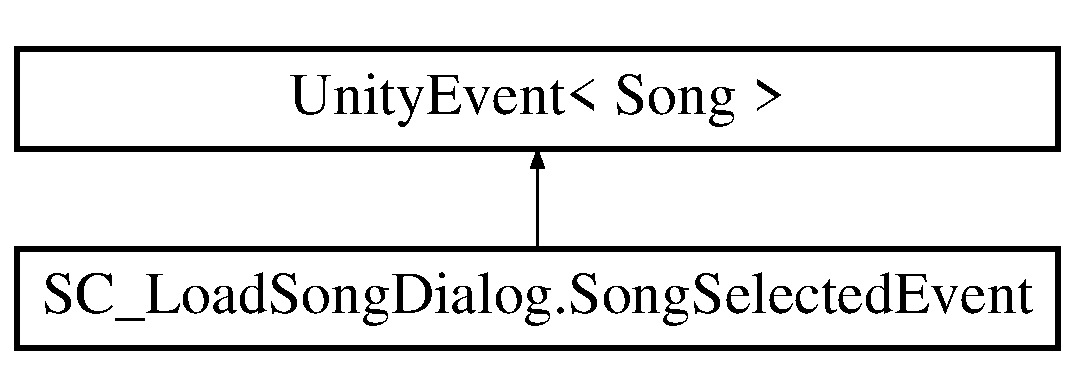
\includegraphics[height=2.000000cm]{group___s_c___l_s_d_event_types}
\end{center}
\end{figure}

\hypertarget{group___white_key_event_types}{}\section{Event Types}
\label{group___white_key_event_types}\index{Event Types@{Event Types}}
\subsection*{Classes}
\begin{DoxyCompactItemize}
\item 
class \hyperlink{group___white_key_event_types_class_white_key_1_1_white_key_pressed_event}{White\+Key.\+White\+Key\+Pressed\+Event}
\item 
class \hyperlink{group___white_key_event_types_class_white_key_1_1_white_key_released_event}{White\+Key.\+White\+Key\+Released\+Event}
\begin{DoxyCompactList}\small\item\em $<$ Used for testing the container. Will probably need to change later.  \hyperlink{group___white_key_event_types_class_white_key_1_1_white_key_released_event}{More...}\end{DoxyCompactList}\end{DoxyCompactItemize}


\subsection{Detailed Description}
The types of events for a \hyperlink{class_white_key}{White\+Key}. 

\subsection{Class Documentation}
\index{White\+Key\+::\+White\+Key\+Pressed\+Event@{White\+Key\+::\+White\+Key\+Pressed\+Event}}\label{class_white_key_1_1_white_key_pressed_event}
\Hypertarget{group___white_key_event_types_class_white_key_1_1_white_key_pressed_event}
\subsubsection{class White\+Key\+:\+:White\+Key\+Pressed\+Event}


Definition at line 23 of file White\+Key.\+cs.

Inheritance diagram for White\+Key.\+White\+Key\+Pressed\+Event\+:\begin{figure}[H]
\begin{center}
\leavevmode
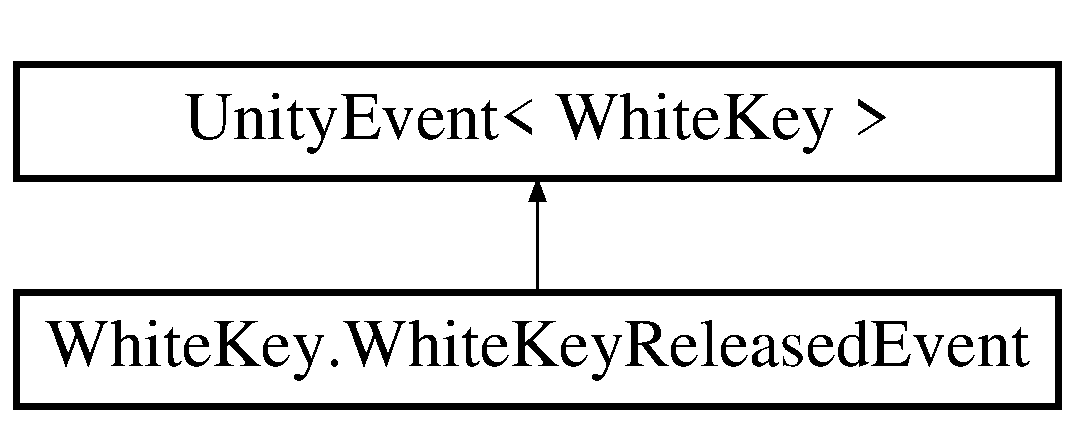
\includegraphics[height=2.000000cm]{group___white_key_event_types}
\end{center}
\end{figure}
\index{White\+Key\+::\+White\+Key\+Released\+Event@{White\+Key\+::\+White\+Key\+Released\+Event}}\label{class_white_key_1_1_white_key_released_event}
\Hypertarget{group___white_key_event_types_class_white_key_1_1_white_key_released_event}
\subsubsection{class White\+Key\+:\+:White\+Key\+Released\+Event}
$<$ Used for testing the container. Will probably need to change later. 

Definition at line 24 of file White\+Key.\+cs.

Inheritance diagram for White\+Key.\+White\+Key\+Released\+Event\+:\begin{figure}[H]
\begin{center}
\leavevmode
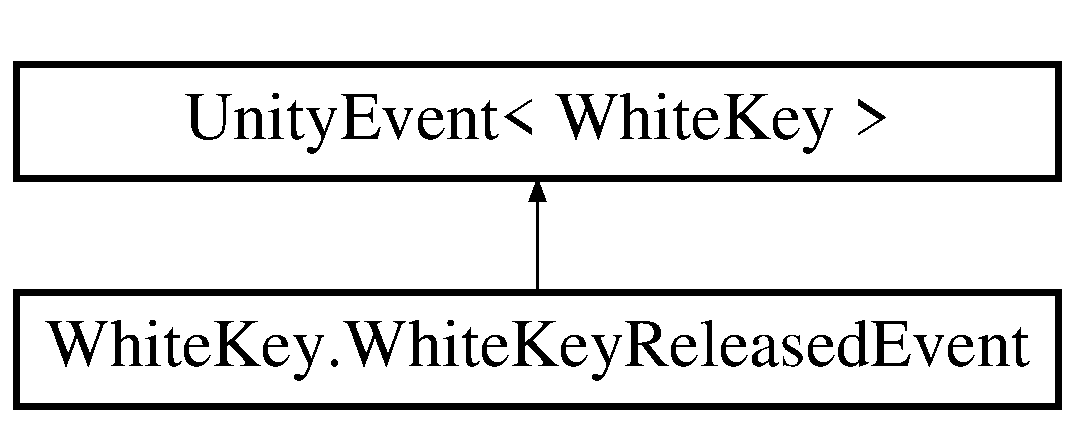
\includegraphics[height=2.000000cm]{group___white_key_event_types}
\end{center}
\end{figure}

\hypertarget{group___v_i_m_event_types}{}\section{Event Types}
\label{group___v_i_m_event_types}\index{Event Types@{Event Types}}
\subsection*{Classes}
\begin{DoxyCompactItemize}
\item 
class \hyperlink{group___v_i_m_event_types_class_virtual_instrument_manager_1_1_audio_finished_event}{Virtual\+Instrument\+Manager.\+Audio\+Finished\+Event}
\begin{DoxyCompactList}\small\item\em Notifies when the audio is finished. There\textquotesingle{}s no handler for this, but it can be used by other classes who need to be notified.  \hyperlink{group___v_i_m_event_types_class_virtual_instrument_manager_1_1_audio_finished_event}{More...}\end{DoxyCompactList}\item 
class \hyperlink{group___v_i_m_event_types_class_virtual_instrument_manager_1_1_change_note_range_event}{Virtual\+Instrument\+Manager.\+Change\+Note\+Range\+Event}
\begin{DoxyCompactList}\small\item\em A type of event that is invoked whenever the range of playable pitches should change.  \hyperlink{group___v_i_m_event_types_class_virtual_instrument_manager_1_1_change_note_range_event}{More...}\end{DoxyCompactList}\item 
class \hyperlink{group___v_i_m_event_types_class_virtual_instrument_manager_1_1_change_instrument_event}{Virtual\+Instrument\+Manager.\+Change\+Instrument\+Event}
\begin{DoxyCompactList}\small\item\em A type of event that is invoked whenever a new instrument should be loaded.  \hyperlink{group___v_i_m_event_types_class_virtual_instrument_manager_1_1_change_instrument_event}{More...}\end{DoxyCompactList}\item 
class \hyperlink{group___v_i_m_event_types_class_virtual_instrument_manager_1_1_drum_kit_loaded_event}{Virtual\+Instrument\+Manager.\+Drum\+Kit\+Loaded\+Event}
\begin{DoxyCompactList}\small\item\em A type of event that is invoked in order to signal that the drum kit has loaded.  \hyperlink{group___v_i_m_event_types_class_virtual_instrument_manager_1_1_drum_kit_loaded_event}{More...}\end{DoxyCompactList}\item 
class \hyperlink{group___v_i_m_event_types_class_virtual_instrument_manager_1_1_instrument_loaded_event}{Virtual\+Instrument\+Manager.\+Instrument\+Loaded\+Event}
\begin{DoxyCompactList}\small\item\em A type of event that is invoked in order to signal that the instrument has loaded.  \hyperlink{group___v_i_m_event_types_class_virtual_instrument_manager_1_1_instrument_loaded_event}{More...}\end{DoxyCompactList}\item 
class \hyperlink{group___v_i_m_event_types_class_virtual_instrument_manager_1_1_modify_echo_filter_event}{Virtual\+Instrument\+Manager.\+Modify\+Echo\+Filter\+Event}
\begin{DoxyCompactList}\small\item\em A type of event that is invoked in order to modify the echo filter.  \hyperlink{group___v_i_m_event_types_class_virtual_instrument_manager_1_1_modify_echo_filter_event}{More...}\end{DoxyCompactList}\item 
class \hyperlink{group___v_i_m_event_types_class_virtual_instrument_manager_1_1_modify_reverb_filter_event}{Virtual\+Instrument\+Manager.\+Modify\+Reverb\+Filter\+Event}
\begin{DoxyCompactList}\small\item\em A type of event that is invoked in order to modify the reverb filter.  \hyperlink{group___v_i_m_event_types_class_virtual_instrument_manager_1_1_modify_reverb_filter_event}{More...}\end{DoxyCompactList}\item 
class \hyperlink{group___v_i_m_event_types_class_virtual_instrument_manager_1_1_pause_drum_loop_event}{Virtual\+Instrument\+Manager.\+Pause\+Drum\+Loop\+Event}
\begin{DoxyCompactList}\small\item\em A type of event that is invoked in order to pause a drum loop.  \hyperlink{group___v_i_m_event_types_class_virtual_instrument_manager_1_1_pause_drum_loop_event}{More...}\end{DoxyCompactList}\item 
class \hyperlink{group___v_i_m_event_types_class_virtual_instrument_manager_1_1_pause_song_event}{Virtual\+Instrument\+Manager.\+Pause\+Song\+Event}
\begin{DoxyCompactList}\small\item\em A type of event that is invoked in order to pause a song.  \hyperlink{group___v_i_m_event_types_class_virtual_instrument_manager_1_1_pause_song_event}{More...}\end{DoxyCompactList}\item 
class \hyperlink{group___v_i_m_event_types_class_virtual_instrument_manager_1_1_play_drum_loop_event}{Virtual\+Instrument\+Manager.\+Play\+Drum\+Loop\+Event}
\begin{DoxyCompactList}\small\item\em A type of event that is invoked in order to play a drum loop.  \hyperlink{group___v_i_m_event_types_class_virtual_instrument_manager_1_1_play_drum_loop_event}{More...}\end{DoxyCompactList}\item 
class \hyperlink{group___v_i_m_event_types_class_virtual_instrument_manager_1_1_play_note_event}{Virtual\+Instrument\+Manager.\+Play\+Note\+Event}
\begin{DoxyCompactList}\small\item\em A type of event that is invoked whenever a note should be played.  \hyperlink{group___v_i_m_event_types_class_virtual_instrument_manager_1_1_play_note_event}{More...}\end{DoxyCompactList}\item 
class \hyperlink{group___v_i_m_event_types_class_virtual_instrument_manager_1_1_play_song_event}{Virtual\+Instrument\+Manager.\+Play\+Song\+Event}
\begin{DoxyCompactList}\small\item\em A type of event that is invoked in order to play a song.  \hyperlink{group___v_i_m_event_types_class_virtual_instrument_manager_1_1_play_song_event}{More...}\end{DoxyCompactList}\item 
class \hyperlink{group___v_i_m_event_types_class_virtual_instrument_manager_1_1_release_note_event}{Virtual\+Instrument\+Manager.\+Release\+Note\+Event}
\begin{DoxyCompactList}\small\item\em A type of event that is invoked whenever a note should fade out as though the key was released.  \hyperlink{group___v_i_m_event_types_class_virtual_instrument_manager_1_1_release_note_event}{More...}\end{DoxyCompactList}\item 
class \hyperlink{group___v_i_m_event_types_class_virtual_instrument_manager_1_1_resume_drum_loop_event}{Virtual\+Instrument\+Manager.\+Resume\+Drum\+Loop\+Event}
\begin{DoxyCompactList}\small\item\em Resumes a drum loop.  \hyperlink{group___v_i_m_event_types_class_virtual_instrument_manager_1_1_resume_drum_loop_event}{More...}\end{DoxyCompactList}\item 
class \hyperlink{group___v_i_m_event_types_class_virtual_instrument_manager_1_1_resume_song_event}{Virtual\+Instrument\+Manager.\+Resume\+Song\+Event}
\begin{DoxyCompactList}\small\item\em Resumes a song.  \hyperlink{group___v_i_m_event_types_class_virtual_instrument_manager_1_1_resume_song_event}{More...}\end{DoxyCompactList}\item 
class \hyperlink{group___v_i_m_event_types_class_virtual_instrument_manager_1_1_stop_drum_loop_event}{Virtual\+Instrument\+Manager.\+Stop\+Drum\+Loop\+Event}
\begin{DoxyCompactList}\small\item\em Stops a drum loop.  \hyperlink{group___v_i_m_event_types_class_virtual_instrument_manager_1_1_stop_drum_loop_event}{More...}\end{DoxyCompactList}\item 
class \hyperlink{group___v_i_m_event_types_class_virtual_instrument_manager_1_1_stop_song_event}{Virtual\+Instrument\+Manager.\+Stop\+Song\+Event}
\begin{DoxyCompactList}\small\item\em Stops a song.  \hyperlink{group___v_i_m_event_types_class_virtual_instrument_manager_1_1_stop_song_event}{More...}\end{DoxyCompactList}\end{DoxyCompactItemize}


\subsection{Detailed Description}
These are classes that inherit from Unity\+Event with varying parameters. They provide a base type for the \hyperlink{group___v_i_m_events}{events } 

\subsection{Class Documentation}
\index{Virtual\+Instrument\+Manager\+::\+Audio\+Finished\+Event@{Virtual\+Instrument\+Manager\+::\+Audio\+Finished\+Event}}\label{class_virtual_instrument_manager_1_1_audio_finished_event}
\Hypertarget{group___v_i_m_event_types_class_virtual_instrument_manager_1_1_audio_finished_event}
\subsubsection{class Virtual\+Instrument\+Manager\+:\+:Audio\+Finished\+Event}
Notifies when the audio is finished. There\textquotesingle{}s no handler for this, but it can be used by other classes who need to be notified. 

Definition at line 52 of file Virtual\+Instrument\+Manager.\+cs.

Inheritance diagram for Virtual\+Instrument\+Manager.\+Audio\+Finished\+Event\+:\begin{figure}[H]
\begin{center}
\leavevmode
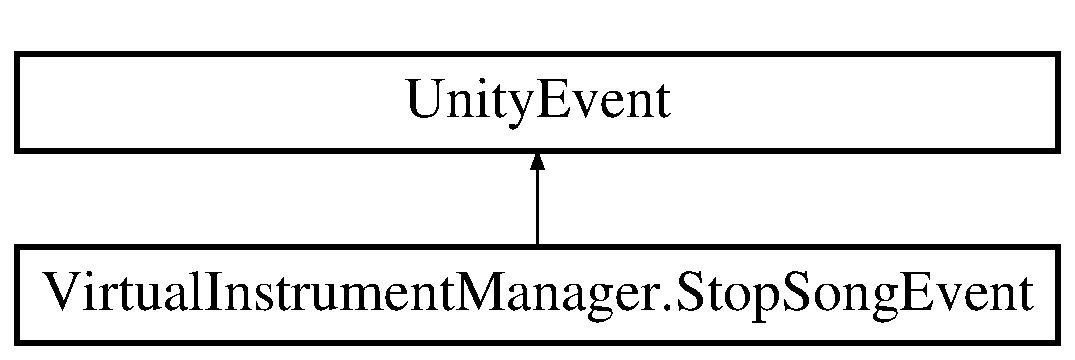
\includegraphics[height=2.000000cm]{group___v_i_m_event_types}
\end{center}
\end{figure}
\index{Virtual\+Instrument\+Manager\+::\+Change\+Note\+Range\+Event@{Virtual\+Instrument\+Manager\+::\+Change\+Note\+Range\+Event}}\label{class_virtual_instrument_manager_1_1_change_note_range_event}
\Hypertarget{group___v_i_m_event_types_class_virtual_instrument_manager_1_1_change_note_range_event}
\subsubsection{class Virtual\+Instrument\+Manager\+:\+:Change\+Note\+Range\+Event}
A type of event that is invoked whenever the range of playable pitches should change. 

The parameter for this type of event is a \hyperlink{group___music_enums_ga508f69b199ea518f935486c990edac1d}{Music.\+P\+I\+T\+CH} which is the lowest pitch of the new range.

\begin{DoxySeeAlso}{See also}
\hyperlink{class_music}{Music} \hyperlink{group___music_enums_ga508f69b199ea518f935486c990edac1d}{Music\+::\+P\+I\+T\+CH} 
\end{DoxySeeAlso}


Definition at line 64 of file Virtual\+Instrument\+Manager.\+cs.

Inheritance diagram for Virtual\+Instrument\+Manager.\+Change\+Note\+Range\+Event\+:\begin{figure}[H]
\begin{center}
\leavevmode
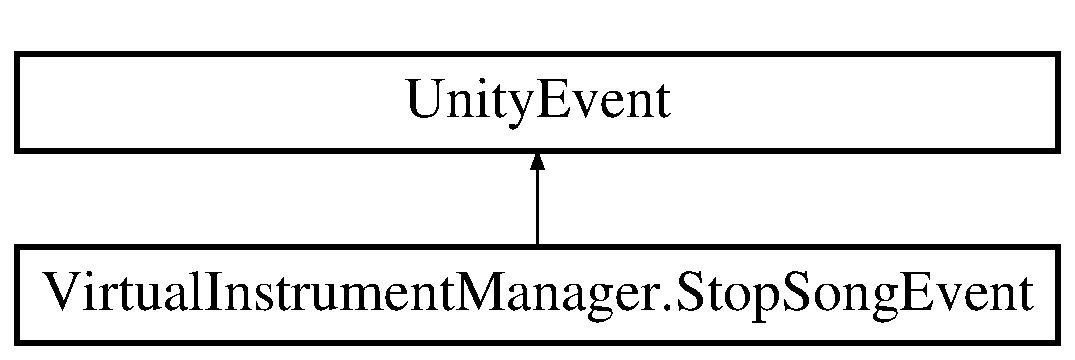
\includegraphics[height=2.000000cm]{group___v_i_m_event_types}
\end{center}
\end{figure}
\index{Virtual\+Instrument\+Manager\+::\+Change\+Instrument\+Event@{Virtual\+Instrument\+Manager\+::\+Change\+Instrument\+Event}}\label{class_virtual_instrument_manager_1_1_change_instrument_event}
\Hypertarget{group___v_i_m_event_types_class_virtual_instrument_manager_1_1_change_instrument_event}
\subsubsection{class Virtual\+Instrument\+Manager\+:\+:Change\+Instrument\+Event}
A type of event that is invoked whenever a new instrument should be loaded. 

The parameter for this type of event is a \hyperlink{group___music_enums_gabfce60192305965558a36e368ebd67c3}{Music.\+I\+N\+S\+T\+R\+U\+M\+E\+N\+T\+\_\+\+T\+Y\+PE} which is the type of instrument that should be loaded.

\begin{DoxySeeAlso}{See also}
\hyperlink{class_music}{Music} \hyperlink{group___music_enums_gabfce60192305965558a36e368ebd67c3}{Music\+::\+I\+N\+S\+T\+R\+U\+M\+E\+N\+T\+\_\+\+T\+Y\+PE} 
\end{DoxySeeAlso}


Definition at line 76 of file Virtual\+Instrument\+Manager.\+cs.

Inheritance diagram for Virtual\+Instrument\+Manager.\+Change\+Instrument\+Event\+:\begin{figure}[H]
\begin{center}
\leavevmode
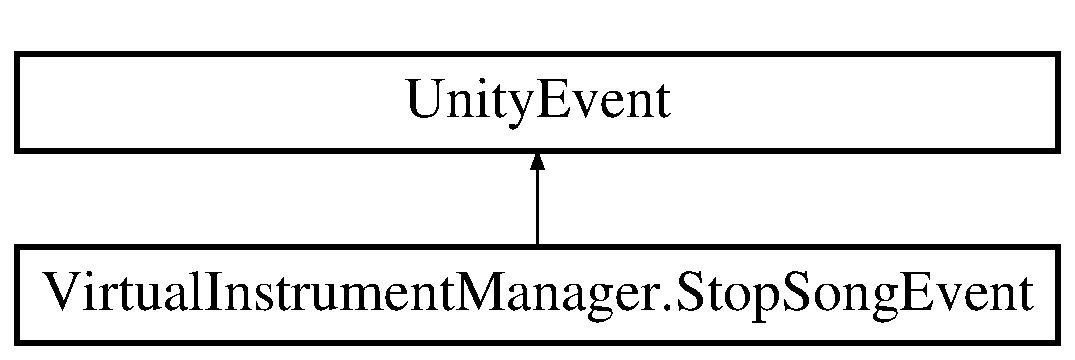
\includegraphics[height=2.000000cm]{group___v_i_m_event_types}
\end{center}
\end{figure}
\index{Virtual\+Instrument\+Manager\+::\+Drum\+Kit\+Loaded\+Event@{Virtual\+Instrument\+Manager\+::\+Drum\+Kit\+Loaded\+Event}}\label{class_virtual_instrument_manager_1_1_drum_kit_loaded_event}
\Hypertarget{group___v_i_m_event_types_class_virtual_instrument_manager_1_1_drum_kit_loaded_event}
\subsubsection{class Virtual\+Instrument\+Manager\+:\+:Drum\+Kit\+Loaded\+Event}
A type of event that is invoked in order to signal that the drum kit has loaded. 

\begin{DoxySeeAlso}{See also}
\hyperlink{group___v_i_m_priv_ga0bc7c9f776b0d2dae0ccb1f1ee5f2143}{Virtual\+Instrument\+Manager\+::m\+Drum\+Kit} \hyperlink{class_drum_kit}{Drum\+Kit} \hyperlink{class_virtual_instrument}{Virtual\+Instrument} 
\end{DoxySeeAlso}


Definition at line 84 of file Virtual\+Instrument\+Manager.\+cs.

Inheritance diagram for Virtual\+Instrument\+Manager.\+Drum\+Kit\+Loaded\+Event\+:\begin{figure}[H]
\begin{center}
\leavevmode
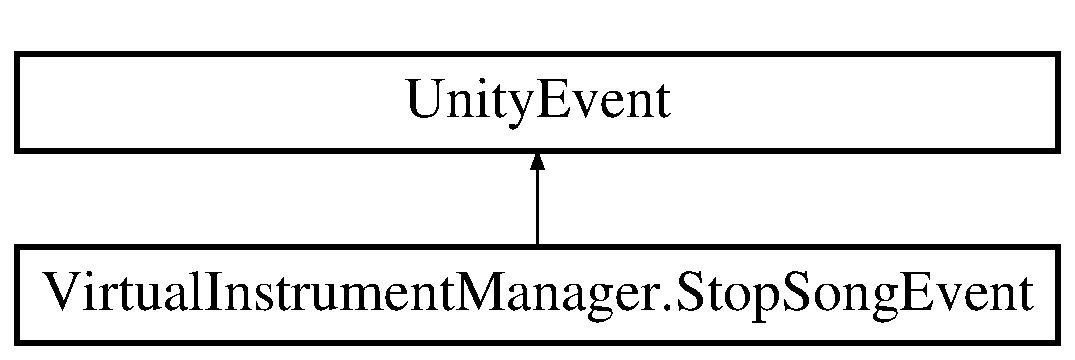
\includegraphics[height=2.000000cm]{group___v_i_m_event_types}
\end{center}
\end{figure}
\index{Virtual\+Instrument\+Manager\+::\+Instrument\+Loaded\+Event@{Virtual\+Instrument\+Manager\+::\+Instrument\+Loaded\+Event}}\label{class_virtual_instrument_manager_1_1_instrument_loaded_event}
\Hypertarget{group___v_i_m_event_types_class_virtual_instrument_manager_1_1_instrument_loaded_event}
\subsubsection{class Virtual\+Instrument\+Manager\+:\+:Instrument\+Loaded\+Event}
A type of event that is invoked in order to signal that the instrument has loaded. 

\begin{DoxySeeAlso}{See also}
\hyperlink{group___v_i_m_priv_gaed435d1f9be09864846db4322dc21fd1}{Virtual\+Instrument\+Manager\+::m\+Instrument} \hyperlink{class_virtual_instrument}{Virtual\+Instrument} 
\end{DoxySeeAlso}


Definition at line 92 of file Virtual\+Instrument\+Manager.\+cs.

Inheritance diagram for Virtual\+Instrument\+Manager.\+Instrument\+Loaded\+Event\+:\begin{figure}[H]
\begin{center}
\leavevmode
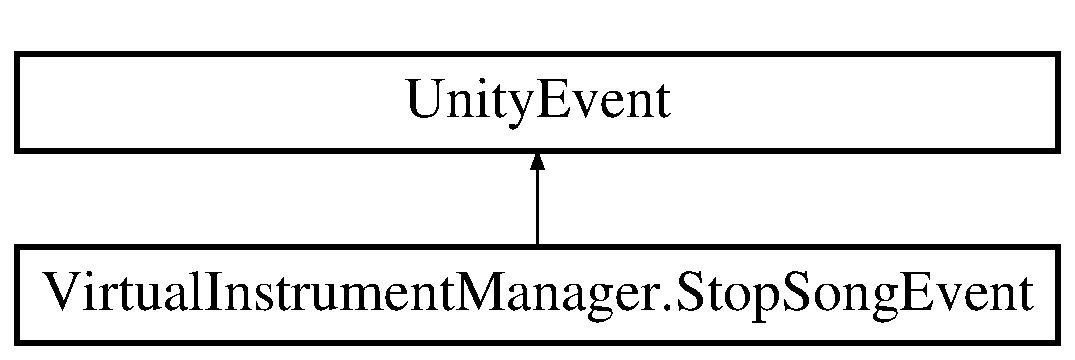
\includegraphics[height=2.000000cm]{group___v_i_m_event_types}
\end{center}
\end{figure}
\index{Virtual\+Instrument\+Manager\+::\+Modify\+Echo\+Filter\+Event@{Virtual\+Instrument\+Manager\+::\+Modify\+Echo\+Filter\+Event}}\label{class_virtual_instrument_manager_1_1_modify_echo_filter_event}
\Hypertarget{group___v_i_m_event_types_class_virtual_instrument_manager_1_1_modify_echo_filter_event}
\subsubsection{class Virtual\+Instrument\+Manager\+:\+:Modify\+Echo\+Filter\+Event}
A type of event that is invoked in order to modify the echo filter. 

The parameter for this type of event is an \hyperlink{group__filter_params_struct_virtual_instrument_manager_1_1_echo_filter_parameters}{Echo\+Filter\+Parameters} struct.

\begin{DoxySeeAlso}{See also}
\hyperlink{group__filter_params_struct_virtual_instrument_manager_1_1_echo_filter_parameters}{Virtual\+Instrument\+Manager\+::\+Echo\+Filter\+Parameters} 
\end{DoxySeeAlso}


Definition at line 103 of file Virtual\+Instrument\+Manager.\+cs.

Inheritance diagram for Virtual\+Instrument\+Manager.\+Modify\+Echo\+Filter\+Event\+:\begin{figure}[H]
\begin{center}
\leavevmode
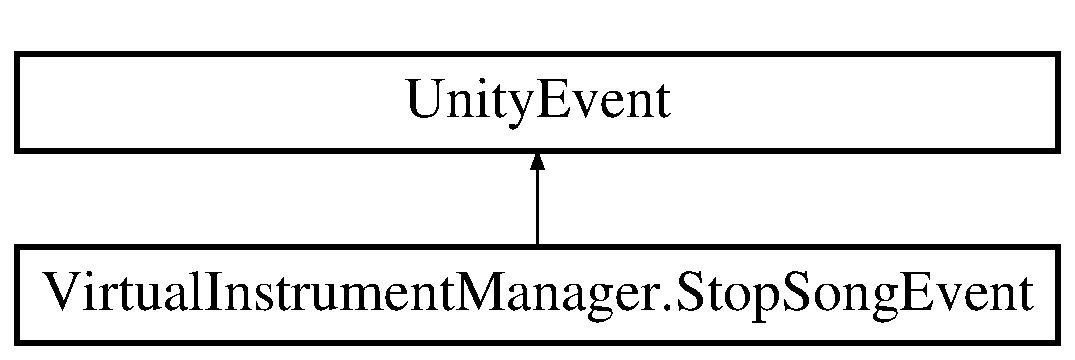
\includegraphics[height=2.000000cm]{group___v_i_m_event_types}
\end{center}
\end{figure}
\index{Virtual\+Instrument\+Manager\+::\+Modify\+Reverb\+Filter\+Event@{Virtual\+Instrument\+Manager\+::\+Modify\+Reverb\+Filter\+Event}}\label{class_virtual_instrument_manager_1_1_modify_reverb_filter_event}
\Hypertarget{group___v_i_m_event_types_class_virtual_instrument_manager_1_1_modify_reverb_filter_event}
\subsubsection{class Virtual\+Instrument\+Manager\+:\+:Modify\+Reverb\+Filter\+Event}
A type of event that is invoked in order to modify the reverb filter. 

The parameter for this type of event is an \hyperlink{group__filter_params_struct_virtual_instrument_manager_1_1_reverb_filter_parameters}{Reverb\+Filter\+Parameters} struct.

\begin{DoxySeeAlso}{See also}
\hyperlink{group__filter_params_struct_virtual_instrument_manager_1_1_reverb_filter_parameters}{Virtual\+Instrument\+Manager\+::\+Reverb\+Filter\+Parameters} 
\end{DoxySeeAlso}


Definition at line 114 of file Virtual\+Instrument\+Manager.\+cs.

Inheritance diagram for Virtual\+Instrument\+Manager.\+Modify\+Reverb\+Filter\+Event\+:\begin{figure}[H]
\begin{center}
\leavevmode
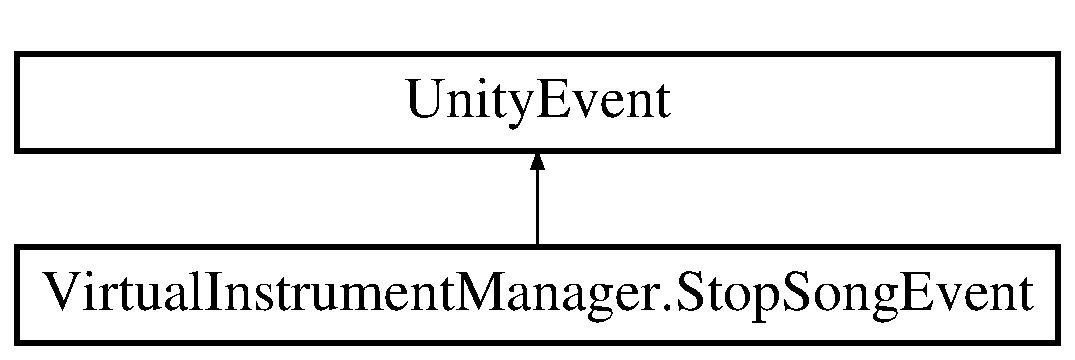
\includegraphics[height=2.000000cm]{group___v_i_m_event_types}
\end{center}
\end{figure}
\index{Virtual\+Instrument\+Manager\+::\+Pause\+Drum\+Loop\+Event@{Virtual\+Instrument\+Manager\+::\+Pause\+Drum\+Loop\+Event}}\label{class_virtual_instrument_manager_1_1_pause_drum_loop_event}
\Hypertarget{group___v_i_m_event_types_class_virtual_instrument_manager_1_1_pause_drum_loop_event}
\subsubsection{class Virtual\+Instrument\+Manager\+:\+:Pause\+Drum\+Loop\+Event}
A type of event that is invoked in order to pause a drum loop. 

\begin{DoxySeeAlso}{See also}
\hyperlink{class_song}{Song} \hyperlink{class_song_manager_class}{Song\+Manager\+Class} \hyperlink{group___n_o_o_pub_func_ga7977bc941f355866c7e4c141a8f7b8bb}{Note\+Output\+Object\+::\+Pause\+Audio} 
\end{DoxySeeAlso}


Definition at line 123 of file Virtual\+Instrument\+Manager.\+cs.

Inheritance diagram for Virtual\+Instrument\+Manager.\+Pause\+Drum\+Loop\+Event\+:\begin{figure}[H]
\begin{center}
\leavevmode
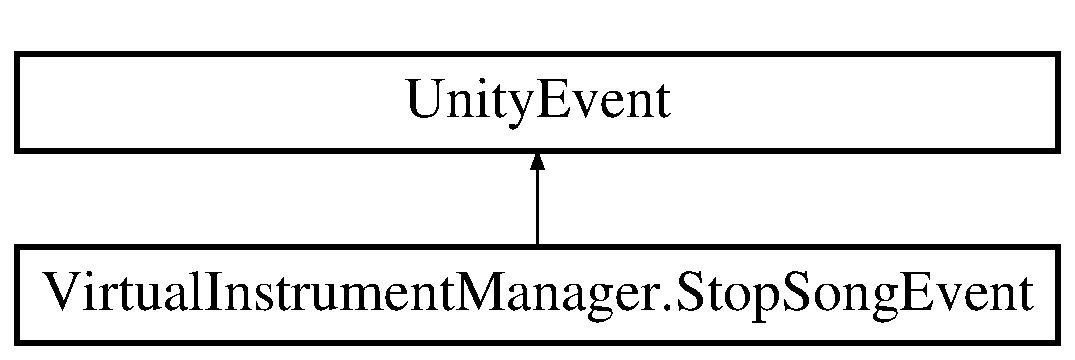
\includegraphics[height=2.000000cm]{group___v_i_m_event_types}
\end{center}
\end{figure}
\index{Virtual\+Instrument\+Manager\+::\+Pause\+Song\+Event@{Virtual\+Instrument\+Manager\+::\+Pause\+Song\+Event}}\label{class_virtual_instrument_manager_1_1_pause_song_event}
\Hypertarget{group___v_i_m_event_types_class_virtual_instrument_manager_1_1_pause_song_event}
\subsubsection{class Virtual\+Instrument\+Manager\+:\+:Pause\+Song\+Event}
A type of event that is invoked in order to pause a song. 

\begin{DoxySeeAlso}{See also}
\hyperlink{class_song}{Song} \hyperlink{class_song_manager_class}{Song\+Manager\+Class} \hyperlink{group___n_o_o_pub_func_ga7977bc941f355866c7e4c141a8f7b8bb}{Note\+Output\+Object\+::\+Pause\+Audio} 
\end{DoxySeeAlso}


Definition at line 132 of file Virtual\+Instrument\+Manager.\+cs.

Inheritance diagram for Virtual\+Instrument\+Manager.\+Pause\+Song\+Event\+:\begin{figure}[H]
\begin{center}
\leavevmode
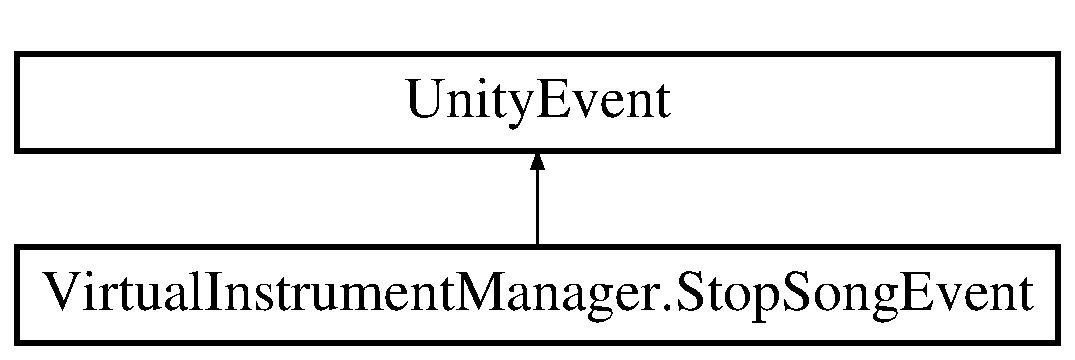
\includegraphics[height=2.000000cm]{group___v_i_m_event_types}
\end{center}
\end{figure}
\index{Virtual\+Instrument\+Manager\+::\+Play\+Drum\+Loop\+Event@{Virtual\+Instrument\+Manager\+::\+Play\+Drum\+Loop\+Event}}\label{class_virtual_instrument_manager_1_1_play_drum_loop_event}
\Hypertarget{group___v_i_m_event_types_class_virtual_instrument_manager_1_1_play_drum_loop_event}
\subsubsection{class Virtual\+Instrument\+Manager\+:\+:Play\+Drum\+Loop\+Event}
A type of event that is invoked in order to play a drum loop. 

The parameter for this type of event is a \hyperlink{class_song}{Song} with the \hyperlink{group___song_enums_ggae681a1f001333e39fc1cb4fea97bfe1ba150deef06b13ddaeac61d0d2699ec61e}{Song\+::\+Song\+Type\+::\+Drum\+Loop}. The song can be obtained from the \hyperlink{class_song_manager_class}{Song\+Manager\+Class}, which the \hyperlink{class_virtual_instrument_manager}{Virtual\+Instrument\+Manager} holds a reference to with \hyperlink{group___v_i_m_pub_ga33dae94932c10c66db76a0eebec76b01}{Virtual\+Instrument\+Manager\+::\+Song\+Manager}.

\begin{DoxySeeAlso}{See also}
\hyperlink{class_song}{Song} \hyperlink{group___song_enums_gae681a1f001333e39fc1cb4fea97bfe1b}{Song\+::\+Song\+Type} \hyperlink{class_song_manager_class}{Song\+Manager\+Class} \hyperlink{group___v_i_m_pub_ga33dae94932c10c66db76a0eebec76b01}{Virtual\+Instrument\+Manager\+::\+Song\+Manager} 
\end{DoxySeeAlso}


Definition at line 145 of file Virtual\+Instrument\+Manager.\+cs.

Inheritance diagram for Virtual\+Instrument\+Manager.\+Play\+Drum\+Loop\+Event\+:\begin{figure}[H]
\begin{center}
\leavevmode
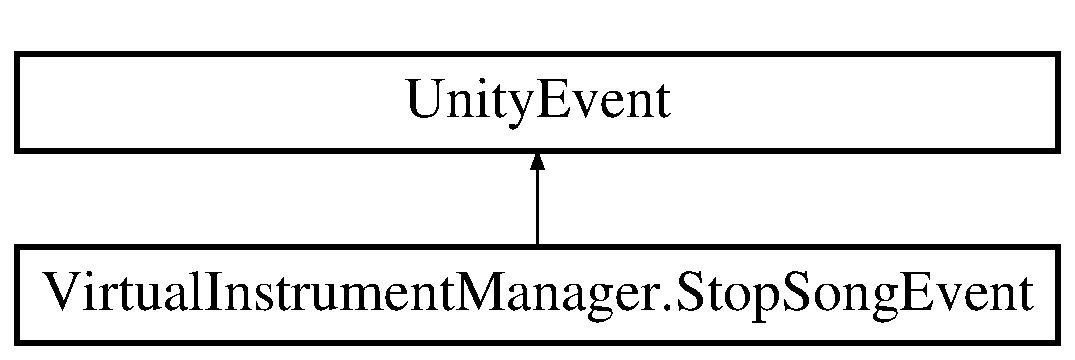
\includegraphics[height=2.000000cm]{group___v_i_m_event_types}
\end{center}
\end{figure}
\index{Virtual\+Instrument\+Manager\+::\+Play\+Note\+Event@{Virtual\+Instrument\+Manager\+::\+Play\+Note\+Event}}\label{class_virtual_instrument_manager_1_1_play_note_event}
\Hypertarget{group___v_i_m_event_types_class_virtual_instrument_manager_1_1_play_note_event}
\subsubsection{class Virtual\+Instrument\+Manager\+:\+:Play\+Note\+Event}
A type of event that is invoked whenever a note should be played. 

The parameters for this type of event are a \hyperlink{group___music_enums_ga508f69b199ea518f935486c990edac1d}{Music.\+P\+I\+T\+CH} which is the pitch of the note to play and an integer which is the velocity at which to play it.

\begin{DoxySeeAlso}{See also}
\hyperlink{class_music}{Music} \hyperlink{group___music_enums_ga508f69b199ea518f935486c990edac1d}{Music\+::\+P\+I\+T\+CH} 
\end{DoxySeeAlso}


Definition at line 157 of file Virtual\+Instrument\+Manager.\+cs.

Inheritance diagram for Virtual\+Instrument\+Manager.\+Play\+Note\+Event\+:\begin{figure}[H]
\begin{center}
\leavevmode
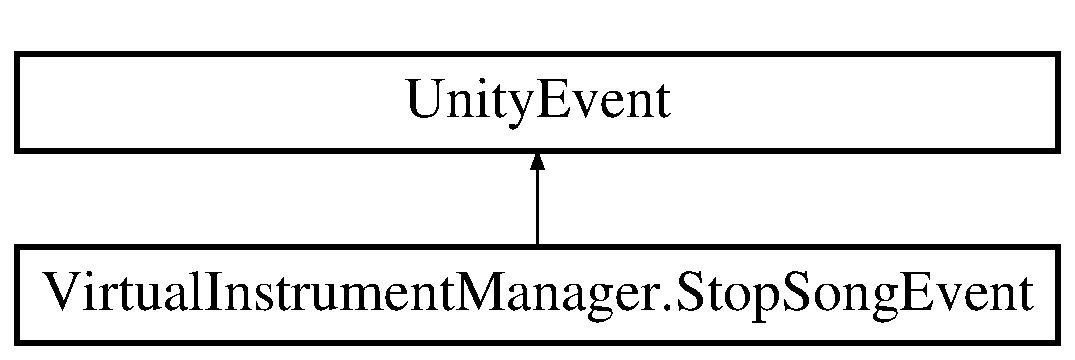
\includegraphics[height=2.000000cm]{group___v_i_m_event_types}
\end{center}
\end{figure}
\index{Virtual\+Instrument\+Manager\+::\+Play\+Song\+Event@{Virtual\+Instrument\+Manager\+::\+Play\+Song\+Event}}\label{class_virtual_instrument_manager_1_1_play_song_event}
\Hypertarget{group___v_i_m_event_types_class_virtual_instrument_manager_1_1_play_song_event}
\subsubsection{class Virtual\+Instrument\+Manager\+:\+:Play\+Song\+Event}
A type of event that is invoked in order to play a song. 

The parameter for this type of event is a \hyperlink{class_song}{Song}. The song can be obtained from the \hyperlink{class_song_manager_class}{Song\+Manager\+Class}, which the \hyperlink{class_virtual_instrument_manager}{Virtual\+Instrument\+Manager} holds a reference to with \hyperlink{group___v_i_m_pub_ga33dae94932c10c66db76a0eebec76b01}{Virtual\+Instrument\+Manager\+::\+Song\+Manager}.

\begin{DoxySeeAlso}{See also}
\hyperlink{class_song}{Song} \hyperlink{class_song_manager_class}{Song\+Manager\+Class} \hyperlink{group___v_i_m_pub_ga33dae94932c10c66db76a0eebec76b01}{Virtual\+Instrument\+Manager\+::\+Song\+Manager} 
\end{DoxySeeAlso}


Definition at line 170 of file Virtual\+Instrument\+Manager.\+cs.

Inheritance diagram for Virtual\+Instrument\+Manager.\+Play\+Song\+Event\+:\begin{figure}[H]
\begin{center}
\leavevmode
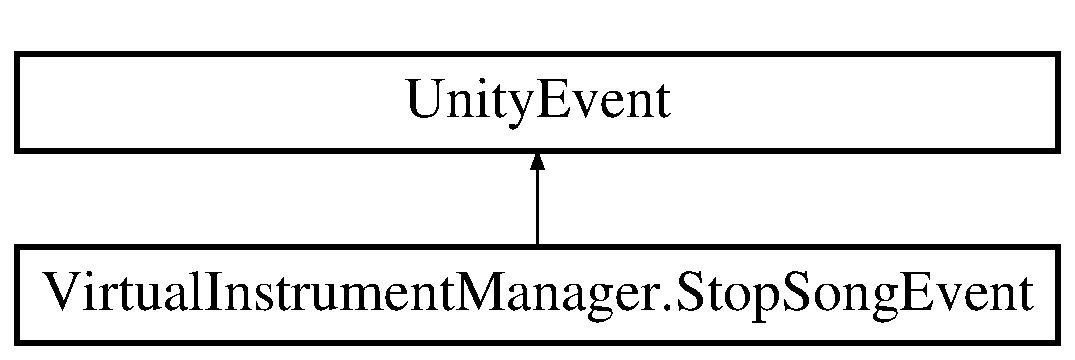
\includegraphics[height=2.000000cm]{group___v_i_m_event_types}
\end{center}
\end{figure}
\index{Virtual\+Instrument\+Manager\+::\+Release\+Note\+Event@{Virtual\+Instrument\+Manager\+::\+Release\+Note\+Event}}\label{class_virtual_instrument_manager_1_1_release_note_event}
\Hypertarget{group___v_i_m_event_types_class_virtual_instrument_manager_1_1_release_note_event}
\subsubsection{class Virtual\+Instrument\+Manager\+:\+:Release\+Note\+Event}
A type of event that is invoked whenever a note should fade out as though the key was released. 

The parameter for this type of event is a \hyperlink{group___music_enums_ga508f69b199ea518f935486c990edac1d}{Music.\+P\+I\+T\+CH} which is the pitch of the note that was released.

\begin{DoxySeeAlso}{See also}
\hyperlink{class_music}{Music} \hyperlink{group___music_enums_ga508f69b199ea518f935486c990edac1d}{Music\+::\+P\+I\+T\+CH} 
\end{DoxySeeAlso}


Definition at line 182 of file Virtual\+Instrument\+Manager.\+cs.

Inheritance diagram for Virtual\+Instrument\+Manager.\+Release\+Note\+Event\+:\begin{figure}[H]
\begin{center}
\leavevmode
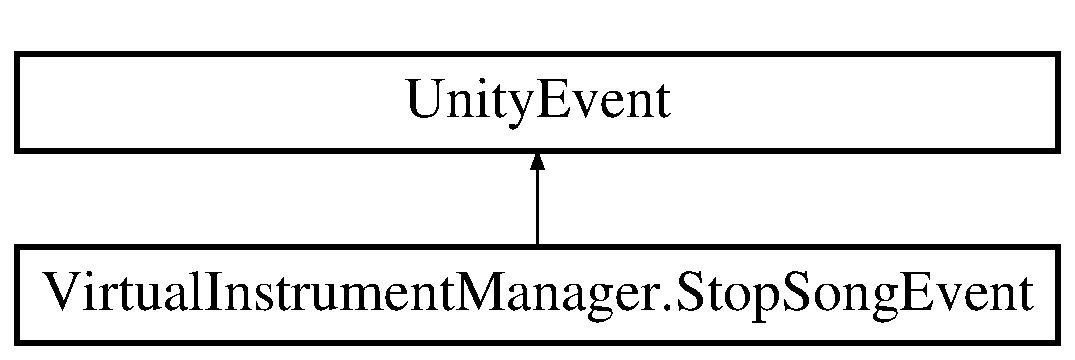
\includegraphics[height=2.000000cm]{group___v_i_m_event_types}
\end{center}
\end{figure}
\index{Virtual\+Instrument\+Manager\+::\+Resume\+Drum\+Loop\+Event@{Virtual\+Instrument\+Manager\+::\+Resume\+Drum\+Loop\+Event}}\label{class_virtual_instrument_manager_1_1_resume_drum_loop_event}
\Hypertarget{group___v_i_m_event_types_class_virtual_instrument_manager_1_1_resume_drum_loop_event}
\subsubsection{class Virtual\+Instrument\+Manager\+:\+:Resume\+Drum\+Loop\+Event}
Resumes a drum loop. 

\begin{DoxySeeAlso}{See also}
\hyperlink{class_song}{Song} \hyperlink{class_song_manager_class}{Song\+Manager\+Class} \hyperlink{group___n_o_o_pub_func_ga2df8edec357dd4123146c9a7e8485ffb}{Note\+Output\+Object\+::\+Resume\+Audio} 
\end{DoxySeeAlso}


Definition at line 191 of file Virtual\+Instrument\+Manager.\+cs.

Inheritance diagram for Virtual\+Instrument\+Manager.\+Resume\+Drum\+Loop\+Event\+:\begin{figure}[H]
\begin{center}
\leavevmode
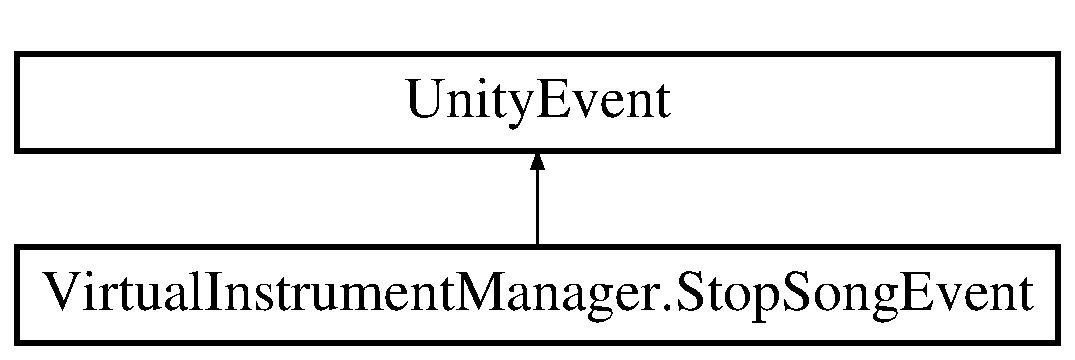
\includegraphics[height=2.000000cm]{group___v_i_m_event_types}
\end{center}
\end{figure}
\index{Virtual\+Instrument\+Manager\+::\+Resume\+Song\+Event@{Virtual\+Instrument\+Manager\+::\+Resume\+Song\+Event}}\label{class_virtual_instrument_manager_1_1_resume_song_event}
\Hypertarget{group___v_i_m_event_types_class_virtual_instrument_manager_1_1_resume_song_event}
\subsubsection{class Virtual\+Instrument\+Manager\+:\+:Resume\+Song\+Event}
Resumes a song. 

\begin{DoxySeeAlso}{See also}
\hyperlink{class_song}{Song} \hyperlink{class_song_manager_class}{Song\+Manager\+Class} \hyperlink{group___n_o_o_pub_func_ga2df8edec357dd4123146c9a7e8485ffb}{Note\+Output\+Object\+::\+Resume\+Audio} 
\end{DoxySeeAlso}


Definition at line 200 of file Virtual\+Instrument\+Manager.\+cs.

Inheritance diagram for Virtual\+Instrument\+Manager.\+Resume\+Song\+Event\+:\begin{figure}[H]
\begin{center}
\leavevmode
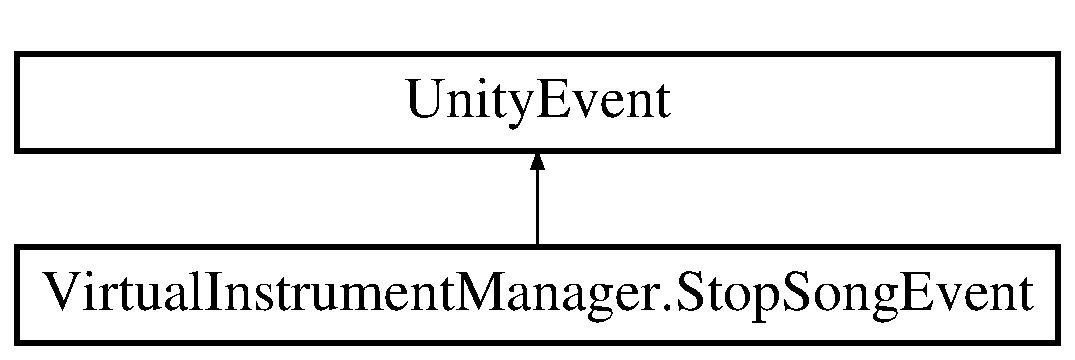
\includegraphics[height=2.000000cm]{group___v_i_m_event_types}
\end{center}
\end{figure}
\index{Virtual\+Instrument\+Manager\+::\+Stop\+Drum\+Loop\+Event@{Virtual\+Instrument\+Manager\+::\+Stop\+Drum\+Loop\+Event}}\label{class_virtual_instrument_manager_1_1_stop_drum_loop_event}
\Hypertarget{group___v_i_m_event_types_class_virtual_instrument_manager_1_1_stop_drum_loop_event}
\subsubsection{class Virtual\+Instrument\+Manager\+:\+:Stop\+Drum\+Loop\+Event}
Stops a drum loop. 

\begin{DoxySeeAlso}{See also}
\hyperlink{class_song}{Song} \hyperlink{class_song_manager_class}{Song\+Manager\+Class} \hyperlink{group___n_o_o_pub_func_gae8a8e5bc027fd0186464a68399a4fecb}{Note\+Output\+Object\+::\+Stop\+Audio} 
\end{DoxySeeAlso}


Definition at line 209 of file Virtual\+Instrument\+Manager.\+cs.

Inheritance diagram for Virtual\+Instrument\+Manager.\+Stop\+Drum\+Loop\+Event\+:\begin{figure}[H]
\begin{center}
\leavevmode
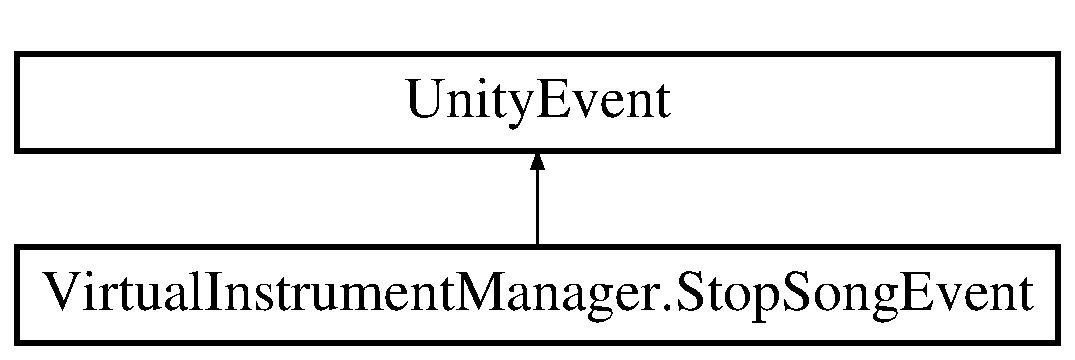
\includegraphics[height=2.000000cm]{group___v_i_m_event_types}
\end{center}
\end{figure}
\index{Virtual\+Instrument\+Manager\+::\+Stop\+Song\+Event@{Virtual\+Instrument\+Manager\+::\+Stop\+Song\+Event}}\label{class_virtual_instrument_manager_1_1_stop_song_event}
\Hypertarget{group___v_i_m_event_types_class_virtual_instrument_manager_1_1_stop_song_event}
\subsubsection{class Virtual\+Instrument\+Manager\+:\+:Stop\+Song\+Event}
Stops a song. 

\begin{DoxySeeAlso}{See also}
\hyperlink{class_song}{Song} \hyperlink{class_song_manager_class}{Song\+Manager\+Class} \hyperlink{group___n_o_o_pub_func_gae8a8e5bc027fd0186464a68399a4fecb}{Note\+Output\+Object\+::\+Stop\+Audio} 
\end{DoxySeeAlso}


Definition at line 218 of file Virtual\+Instrument\+Manager.\+cs.

Inheritance diagram for Virtual\+Instrument\+Manager.\+Stop\+Song\+Event\+:\begin{figure}[H]
\begin{center}
\leavevmode
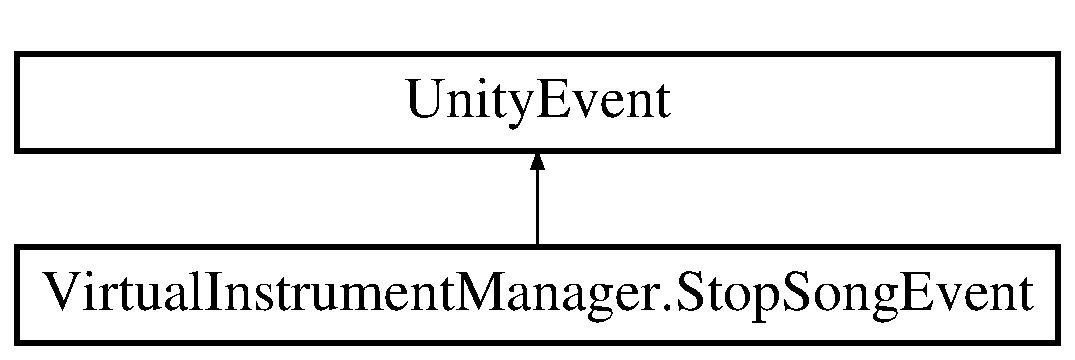
\includegraphics[height=2.000000cm]{group___v_i_m_event_types}
\end{center}
\end{figure}

\hypertarget{group___black_key_event_types}{}\section{Event Types}
\label{group___black_key_event_types}\index{Event Types@{Event Types}}
\subsection*{Classes}
\begin{DoxyCompactItemize}
\item 
class \hyperlink{group___black_key_event_types_class_black_key_1_1_black_key_pressed_event}{Black\+Key.\+Black\+Key\+Pressed\+Event}
\item 
class \hyperlink{group___black_key_event_types_class_black_key_1_1_black_key_released_event}{Black\+Key.\+Black\+Key\+Released\+Event}
\begin{DoxyCompactList}\small\item\em $<$ Used for testing the container. Will probably need to change later.  \hyperlink{group___black_key_event_types_class_black_key_1_1_black_key_released_event}{More...}\end{DoxyCompactList}\end{DoxyCompactItemize}


\subsection{Detailed Description}
The types of events for the \hyperlink{group___doc_black_key}{black keys}. 

\subsection{Class Documentation}
\index{Black\+Key\+::\+Black\+Key\+Pressed\+Event@{Black\+Key\+::\+Black\+Key\+Pressed\+Event}}\label{class_black_key_1_1_black_key_pressed_event}
\Hypertarget{group___black_key_event_types_class_black_key_1_1_black_key_pressed_event}
\subsubsection{class Black\+Key\+:\+:Black\+Key\+Pressed\+Event}


Definition at line 23 of file Black\+Key.\+cs.

Inheritance diagram for Black\+Key.\+Black\+Key\+Pressed\+Event\+:\begin{figure}[H]
\begin{center}
\leavevmode
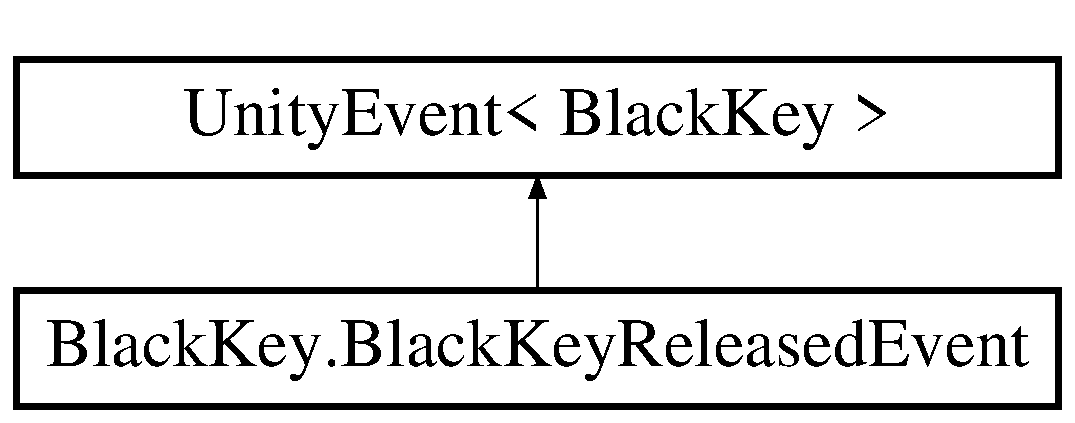
\includegraphics[height=2.000000cm]{group___black_key_event_types}
\end{center}
\end{figure}
\index{Black\+Key\+::\+Black\+Key\+Released\+Event@{Black\+Key\+::\+Black\+Key\+Released\+Event}}\label{class_black_key_1_1_black_key_released_event}
\Hypertarget{group___black_key_event_types_class_black_key_1_1_black_key_released_event}
\subsubsection{class Black\+Key\+:\+:Black\+Key\+Released\+Event}
$<$ Used for testing the container. Will probably need to change later. 

Definition at line 24 of file Black\+Key.\+cs.

Inheritance diagram for Black\+Key.\+Black\+Key\+Released\+Event\+:\begin{figure}[H]
\begin{center}
\leavevmode
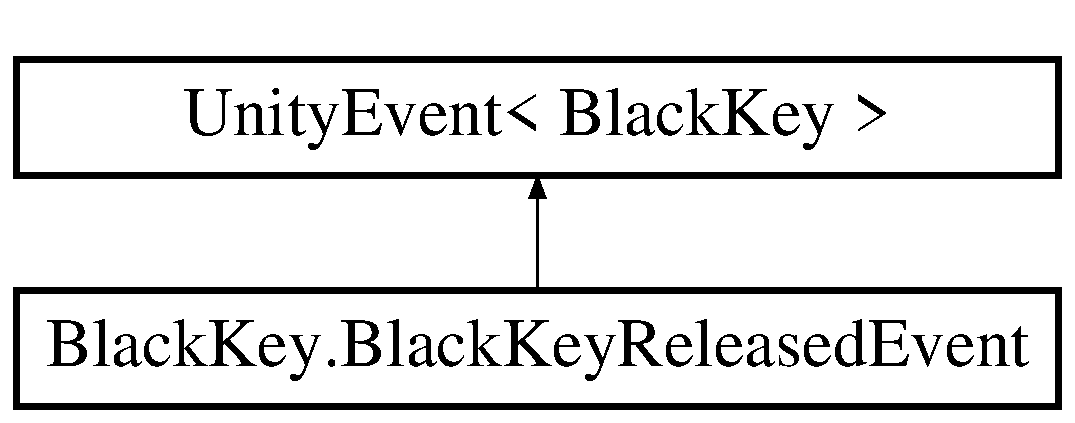
\includegraphics[height=2.000000cm]{group___black_key_event_types}
\end{center}
\end{figure}

\hypertarget{group___white_key_events}{}\section{Events}
\label{group___white_key_events}\index{Events@{Events}}
\subsection*{Variables}
\begin{DoxyCompactItemize}
\item 
\hyperlink{group___white_key_event_types_class_white_key_1_1_white_key_pressed_event}{White\+Key\+Pressed\+Event} \hyperlink{group___white_key_events_gab84691fc1e9f7b62884589d1813433e2}{White\+Key.\+White\+Key\+Pressed} = null
\begin{DoxyCompactList}\small\item\em Used for testing the container. Will probably need to change later. \end{DoxyCompactList}\item 
\hyperlink{group___white_key_event_types_class_white_key_1_1_white_key_released_event}{White\+Key\+Released\+Event} \hyperlink{group___white_key_events_ga180e88cd7ab95af43231f53469e87830}{White\+Key.\+White\+Key\+Released} = null
\begin{DoxyCompactList}\small\item\em Used for testing the container. Will probably need to change later. \end{DoxyCompactList}\end{DoxyCompactItemize}


\subsection{Detailed Description}
Events used by the \hyperlink{class_white_key}{White\+Key}. 

\subsection{Variable Documentation}
\mbox{\Hypertarget{group___white_key_events_gab84691fc1e9f7b62884589d1813433e2}\label{group___white_key_events_gab84691fc1e9f7b62884589d1813433e2}} 
\index{Events@{Events}!White\+Key\+Pressed@{White\+Key\+Pressed}}
\index{White\+Key\+Pressed@{White\+Key\+Pressed}!Events@{Events}}
\subsubsection{\texorpdfstring{White\+Key\+Pressed}{WhiteKeyPressed}}
{\footnotesize\ttfamily \hyperlink{group___white_key_event_types_class_white_key_1_1_white_key_pressed_event}{White\+Key\+Pressed\+Event} White\+Key.\+White\+Key\+Pressed = null}



Used for testing the container. Will probably need to change later. 



Definition at line 33 of file White\+Key.\+cs.



Referenced by Key\+Container.\+Load\+Keys().

\mbox{\Hypertarget{group___white_key_events_ga180e88cd7ab95af43231f53469e87830}\label{group___white_key_events_ga180e88cd7ab95af43231f53469e87830}} 
\index{Events@{Events}!White\+Key\+Released@{White\+Key\+Released}}
\index{White\+Key\+Released@{White\+Key\+Released}!Events@{Events}}
\subsubsection{\texorpdfstring{White\+Key\+Released}{WhiteKeyReleased}}
{\footnotesize\ttfamily \hyperlink{group___white_key_event_types_class_white_key_1_1_white_key_released_event}{White\+Key\+Released\+Event} White\+Key.\+White\+Key\+Released = null}



Used for testing the container. Will probably need to change later. 



Definition at line 34 of file White\+Key.\+cs.



Referenced by Key\+Container.\+Load\+Keys().


\hypertarget{group___s_c___l_s_d_events}{}\section{Events}
\label{group___s_c___l_s_d_events}\index{Events@{Events}}
\subsection*{Variables}
\begin{DoxyCompactItemize}
\item 
\hyperlink{group___s_c___l_s_d_event_types_class_s_c___load_song_dialog_1_1_song_selected_event}{Song\+Selected\+Event} \hyperlink{group___s_c___l_s_d_events_ga48d606b2c8291fee822dcc2b14ddcecc}{S\+C\+\_\+\+Load\+Song\+Dialog.\+Song\+Selected}
\begin{DoxyCompactList}\small\item\em The event that is invoked when a song is selected. No handler for this event in this class. It\textquotesingle{}s meant to notify other classes. \end{DoxyCompactList}\end{DoxyCompactItemize}


\subsection{Detailed Description}
These are the events for the \hyperlink{group___doc_s_c___l_s_d}{dialog to load a song}. 

\subsection{Variable Documentation}
\mbox{\Hypertarget{group___s_c___l_s_d_events_ga48d606b2c8291fee822dcc2b14ddcecc}\label{group___s_c___l_s_d_events_ga48d606b2c8291fee822dcc2b14ddcecc}} 
\index{Events@{Events}!Song\+Selected@{Song\+Selected}}
\index{Song\+Selected@{Song\+Selected}!Events@{Events}}
\subsubsection{\texorpdfstring{Song\+Selected}{SongSelected}}
{\footnotesize\ttfamily \hyperlink{group___s_c___l_s_d_event_types_class_s_c___load_song_dialog_1_1_song_selected_event}{Song\+Selected\+Event} S\+C\+\_\+\+Load\+Song\+Dialog.\+Song\+Selected}



The event that is invoked when a song is selected. No handler for this event in this class. It\textquotesingle{}s meant to notify other classes. 



Definition at line 37 of file S\+C\+\_\+\+Load\+Song\+Dialog.\+cs.



Referenced by Song\+Creation\+Manager.\+On\+Load\+Song\+Button\+Clicked().


\hypertarget{group___black_key_events}{}\section{Events}
\label{group___black_key_events}\index{Events@{Events}}
\subsection*{Variables}
\begin{DoxyCompactItemize}
\item 
\hyperlink{group___black_key_event_types_class_black_key_1_1_black_key_pressed_event}{Black\+Key\+Pressed\+Event} \hyperlink{group___black_key_events_ga51f1badf49df0c54e31a20ba4b7abd6b}{Black\+Key.\+Black\+Key\+Pressed} = null
\begin{DoxyCompactList}\small\item\em Used for testing the container. Will probably need to change later. \end{DoxyCompactList}\item 
\hyperlink{group___black_key_event_types_class_black_key_1_1_black_key_released_event}{Black\+Key\+Released\+Event} \hyperlink{group___black_key_events_ga2710bdaba16dbdb82c0d38f11ce642d8}{Black\+Key.\+Black\+Key\+Released} = null
\begin{DoxyCompactList}\small\item\em Used for testing the container. Will probably need to change later. \end{DoxyCompactList}\end{DoxyCompactItemize}


\subsection{Detailed Description}
Events used by the \hyperlink{group___doc_black_key}{black keys} 

\subsection{Variable Documentation}
\mbox{\Hypertarget{group___black_key_events_ga51f1badf49df0c54e31a20ba4b7abd6b}\label{group___black_key_events_ga51f1badf49df0c54e31a20ba4b7abd6b}} 
\index{Events@{Events}!Black\+Key\+Pressed@{Black\+Key\+Pressed}}
\index{Black\+Key\+Pressed@{Black\+Key\+Pressed}!Events@{Events}}
\subsubsection{\texorpdfstring{Black\+Key\+Pressed}{BlackKeyPressed}}
{\footnotesize\ttfamily \hyperlink{group___black_key_event_types_class_black_key_1_1_black_key_pressed_event}{Black\+Key\+Pressed\+Event} Black\+Key.\+Black\+Key\+Pressed = null}



Used for testing the container. Will probably need to change later. 



Definition at line 33 of file Black\+Key.\+cs.



Referenced by Key\+Container.\+Load\+Keys().

\mbox{\Hypertarget{group___black_key_events_ga2710bdaba16dbdb82c0d38f11ce642d8}\label{group___black_key_events_ga2710bdaba16dbdb82c0d38f11ce642d8}} 
\index{Events@{Events}!Black\+Key\+Released@{Black\+Key\+Released}}
\index{Black\+Key\+Released@{Black\+Key\+Released}!Events@{Events}}
\subsubsection{\texorpdfstring{Black\+Key\+Released}{BlackKeyReleased}}
{\footnotesize\ttfamily \hyperlink{group___black_key_event_types_class_black_key_1_1_black_key_released_event}{Black\+Key\+Released\+Event} Black\+Key.\+Black\+Key\+Released = null}



Used for testing the container. Will probably need to change later. 



Definition at line 34 of file Black\+Key.\+cs.



Referenced by Key\+Container.\+Load\+Keys().


\hypertarget{group___v_i_m_events}{}\section{Events}
\label{group___v_i_m_events}\index{Events@{Events}}
\subsection*{Variables}
\begin{DoxyCompactItemize}
\item 
\hyperlink{group___v_i_m_event_types_class_virtual_instrument_manager_1_1_audio_finished_event}{Audio\+Finished\+Event} \hyperlink{group___v_i_m_events_ga39ffa8215ab5c9ad46c563e2bd87c219}{Virtual\+Instrument\+Manager.\+Audio\+Finished}
\item 
\hyperlink{group___v_i_m_event_types_class_virtual_instrument_manager_1_1_change_note_range_event}{Change\+Note\+Range\+Event} \hyperlink{group___v_i_m_events_gab6fa99d08e8466406835b9fc4ff859f1}{Virtual\+Instrument\+Manager.\+Change\+Note\+Range}
\item 
\hyperlink{group___v_i_m_event_types_class_virtual_instrument_manager_1_1_change_instrument_event}{Change\+Instrument\+Event} \hyperlink{group___v_i_m_events_ga1b9f12a73a5418ea5695d38b78c506c4}{Virtual\+Instrument\+Manager.\+Change\+Instrument}
\item 
\hyperlink{group___v_i_m_event_types_class_virtual_instrument_manager_1_1_drum_kit_loaded_event}{Drum\+Kit\+Loaded\+Event} \hyperlink{group___v_i_m_events_ga2dea060b2fba524166433300113dc281}{Virtual\+Instrument\+Manager.\+Drum\+Kit\+Loaded}
\item 
\hyperlink{group___v_i_m_event_types_class_virtual_instrument_manager_1_1_instrument_loaded_event}{Instrument\+Loaded\+Event} \hyperlink{group___v_i_m_events_gad79b789b020d7e4a8c149ec653c0b97f}{Virtual\+Instrument\+Manager.\+Instrument\+Loaded}
\item 
\hyperlink{group___v_i_m_event_types_class_virtual_instrument_manager_1_1_modify_echo_filter_event}{Modify\+Echo\+Filter\+Event} \hyperlink{group___v_i_m_events_ga112ed15f48fd261f1ad71c3c953c0a58}{Virtual\+Instrument\+Manager.\+Modify\+Echo\+Filter}
\item 
\hyperlink{group___v_i_m_event_types_class_virtual_instrument_manager_1_1_modify_reverb_filter_event}{Modify\+Reverb\+Filter\+Event} \hyperlink{group___v_i_m_events_gaadd137e073cb3849f610a46e0d032858}{Virtual\+Instrument\+Manager.\+Modify\+Reverb\+Filter}
\item 
\hyperlink{group___v_i_m_event_types_class_virtual_instrument_manager_1_1_pause_drum_loop_event}{Pause\+Drum\+Loop\+Event} \hyperlink{group___v_i_m_events_ga6de00a430321852cc3c8c4a213d62c70}{Virtual\+Instrument\+Manager.\+Pause\+Drum\+Loop}
\item 
\hyperlink{group___v_i_m_event_types_class_virtual_instrument_manager_1_1_pause_song_event}{Pause\+Song\+Event} \hyperlink{group___v_i_m_events_gae2d76fc98161d7a4573628dbd93e7887}{Virtual\+Instrument\+Manager.\+Pause\+Song}
\item 
\hyperlink{group___v_i_m_event_types_class_virtual_instrument_manager_1_1_play_drum_loop_event}{Play\+Drum\+Loop\+Event} \hyperlink{group___v_i_m_events_ga5657ff4bcc7de6d240d7092ffd22a6fe}{Virtual\+Instrument\+Manager.\+Play\+Drum\+Loop}
\item 
\hyperlink{group___v_i_m_event_types_class_virtual_instrument_manager_1_1_play_note_event}{Play\+Note\+Event} \hyperlink{group___v_i_m_events_gaa21021c13a8c9d13cbf374d5bf9d68fa}{Virtual\+Instrument\+Manager.\+Play\+Note}
\item 
\hyperlink{group___v_i_m_event_types_class_virtual_instrument_manager_1_1_play_song_event}{Play\+Song\+Event} \hyperlink{group___v_i_m_events_gae450bdba9c513ab4e43f69def50fa84d}{Virtual\+Instrument\+Manager.\+Play\+Song}
\item 
\hyperlink{group___v_i_m_event_types_class_virtual_instrument_manager_1_1_release_note_event}{Release\+Note\+Event} \hyperlink{group___v_i_m_events_ga3a1726a6366126421434c2c7be5e5678}{Virtual\+Instrument\+Manager.\+Release\+Note}
\item 
\hyperlink{group___v_i_m_event_types_class_virtual_instrument_manager_1_1_resume_drum_loop_event}{Resume\+Drum\+Loop\+Event} \hyperlink{group___v_i_m_events_ga54db2dc24076cd3cd130e95c2fd5bea0}{Virtual\+Instrument\+Manager.\+Resume\+Drum\+Loop}
\item 
\hyperlink{group___v_i_m_event_types_class_virtual_instrument_manager_1_1_resume_song_event}{Resume\+Song\+Event} \hyperlink{group___v_i_m_events_ga01670916ae3917c84a0fb51667f30ab9}{Virtual\+Instrument\+Manager.\+Resume\+Song}
\item 
\hyperlink{group___v_i_m_event_types_class_virtual_instrument_manager_1_1_stop_drum_loop_event}{Stop\+Drum\+Loop\+Event} \hyperlink{group___v_i_m_events_ga9466995fd3b4a07351a8577042ee8b31}{Virtual\+Instrument\+Manager.\+Stop\+Drum\+Loop}
\item 
\hyperlink{group___v_i_m_event_types_class_virtual_instrument_manager_1_1_stop_song_event}{Stop\+Song\+Event} \hyperlink{group___v_i_m_events_gaa9e464629814abf2e4db88e240fac72c}{Virtual\+Instrument\+Manager.\+Stop\+Song}
\end{DoxyCompactItemize}


\subsection{Detailed Description}
These are the events that are used to iteract with the \hyperlink{class_virtual_instrument_manager}{Virtual\+Instrument\+Manager}. 

\subsection{Variable Documentation}
\mbox{\Hypertarget{group___v_i_m_events_ga39ffa8215ab5c9ad46c563e2bd87c219}\label{group___v_i_m_events_ga39ffa8215ab5c9ad46c563e2bd87c219}} 
\index{Events@{Events}!Audio\+Finished@{Audio\+Finished}}
\index{Audio\+Finished@{Audio\+Finished}!Events@{Events}}
\subsubsection{\texorpdfstring{Audio\+Finished}{AudioFinished}}
{\footnotesize\ttfamily \hyperlink{group___v_i_m_event_types_class_virtual_instrument_manager_1_1_audio_finished_event}{Audio\+Finished\+Event} Virtual\+Instrument\+Manager.\+Audio\+Finished}

\begin{DoxySeeAlso}{See also}
\hyperlink{group___v_i_m_event_types_class_virtual_instrument_manager_1_1_audio_finished_event}{Virtual\+Instrument\+Manager\+::\+Audio\+Finished\+Event} 
\end{DoxySeeAlso}


Definition at line 282 of file Virtual\+Instrument\+Manager.\+cs.



Referenced by Note\+Output\+Object.\+On\+Audio\+Filter\+Read().

\mbox{\Hypertarget{group___v_i_m_events_ga1b9f12a73a5418ea5695d38b78c506c4}\label{group___v_i_m_events_ga1b9f12a73a5418ea5695d38b78c506c4}} 
\index{Events@{Events}!Change\+Instrument@{Change\+Instrument}}
\index{Change\+Instrument@{Change\+Instrument}!Events@{Events}}
\subsubsection{\texorpdfstring{Change\+Instrument}{ChangeInstrument}}
{\footnotesize\ttfamily \hyperlink{group___v_i_m_event_types_class_virtual_instrument_manager_1_1_change_instrument_event}{Change\+Instrument\+Event} Virtual\+Instrument\+Manager.\+Change\+Instrument}

\begin{DoxySeeAlso}{See also}
\hyperlink{group___v_i_m_event_types_class_virtual_instrument_manager_1_1_change_instrument_event}{Virtual\+Instrument\+Manager\+::\+Change\+Instrument\+Event} 
\end{DoxySeeAlso}


Definition at line 284 of file Virtual\+Instrument\+Manager.\+cs.



Referenced by A\+T\+I\+\_\+\+Instrument\+Selection\+Handler.\+On\+Instrument\+Selected(), and A\+T\+I\+\_\+\+Demo\+Song\+Button\+Handler.\+Start().

\mbox{\Hypertarget{group___v_i_m_events_gab6fa99d08e8466406835b9fc4ff859f1}\label{group___v_i_m_events_gab6fa99d08e8466406835b9fc4ff859f1}} 
\index{Events@{Events}!Change\+Note\+Range@{Change\+Note\+Range}}
\index{Change\+Note\+Range@{Change\+Note\+Range}!Events@{Events}}
\subsubsection{\texorpdfstring{Change\+Note\+Range}{ChangeNoteRange}}
{\footnotesize\ttfamily \hyperlink{group___v_i_m_event_types_class_virtual_instrument_manager_1_1_change_note_range_event}{Change\+Note\+Range\+Event} Virtual\+Instrument\+Manager.\+Change\+Note\+Range}

\begin{DoxySeeAlso}{See also}
\hyperlink{group___v_i_m_event_types_class_virtual_instrument_manager_1_1_change_note_range_event}{Virtual\+Instrument\+Manager\+::\+Change\+Note\+Range\+Event} 
\end{DoxySeeAlso}


Definition at line 283 of file Virtual\+Instrument\+Manager.\+cs.



Referenced by A\+T\+I\+\_\+\+Note\+Range\+Selection\+Handler.\+Handle\+Note\+Range\+Change(), and Key\+Container.\+Update().

\mbox{\Hypertarget{group___v_i_m_events_ga2dea060b2fba524166433300113dc281}\label{group___v_i_m_events_ga2dea060b2fba524166433300113dc281}} 
\index{Events@{Events}!Drum\+Kit\+Loaded@{Drum\+Kit\+Loaded}}
\index{Drum\+Kit\+Loaded@{Drum\+Kit\+Loaded}!Events@{Events}}
\subsubsection{\texorpdfstring{Drum\+Kit\+Loaded}{DrumKitLoaded}}
{\footnotesize\ttfamily \hyperlink{group___v_i_m_event_types_class_virtual_instrument_manager_1_1_drum_kit_loaded_event}{Drum\+Kit\+Loaded\+Event} Virtual\+Instrument\+Manager.\+Drum\+Kit\+Loaded}

\begin{DoxySeeAlso}{See also}
\hyperlink{group___v_i_m_event_types_class_virtual_instrument_manager_1_1_drum_kit_loaded_event}{Virtual\+Instrument\+Manager\+::\+Drum\+Kit\+Loaded\+Event} 
\end{DoxySeeAlso}


Definition at line 285 of file Virtual\+Instrument\+Manager.\+cs.

\mbox{\Hypertarget{group___v_i_m_events_gad79b789b020d7e4a8c149ec653c0b97f}\label{group___v_i_m_events_gad79b789b020d7e4a8c149ec653c0b97f}} 
\index{Events@{Events}!Instrument\+Loaded@{Instrument\+Loaded}}
\index{Instrument\+Loaded@{Instrument\+Loaded}!Events@{Events}}
\subsubsection{\texorpdfstring{Instrument\+Loaded}{InstrumentLoaded}}
{\footnotesize\ttfamily \hyperlink{group___v_i_m_event_types_class_virtual_instrument_manager_1_1_instrument_loaded_event}{Instrument\+Loaded\+Event} Virtual\+Instrument\+Manager.\+Instrument\+Loaded}

\begin{DoxySeeAlso}{See also}
\hyperlink{group___v_i_m_event_types_class_virtual_instrument_manager_1_1_instrument_loaded_event}{Virtual\+Instrument\+Manager\+::\+Instrument\+Loaded\+Event} 
\end{DoxySeeAlso}


Definition at line 286 of file Virtual\+Instrument\+Manager.\+cs.



Referenced by A\+T\+I\+\_\+\+Note\+Range\+Selection\+Handler.\+Start().

\mbox{\Hypertarget{group___v_i_m_events_ga112ed15f48fd261f1ad71c3c953c0a58}\label{group___v_i_m_events_ga112ed15f48fd261f1ad71c3c953c0a58}} 
\index{Events@{Events}!Modify\+Echo\+Filter@{Modify\+Echo\+Filter}}
\index{Modify\+Echo\+Filter@{Modify\+Echo\+Filter}!Events@{Events}}
\subsubsection{\texorpdfstring{Modify\+Echo\+Filter}{ModifyEchoFilter}}
{\footnotesize\ttfamily \hyperlink{group___v_i_m_event_types_class_virtual_instrument_manager_1_1_modify_echo_filter_event}{Modify\+Echo\+Filter\+Event} Virtual\+Instrument\+Manager.\+Modify\+Echo\+Filter}

\begin{DoxySeeAlso}{See also}
\hyperlink{group___v_i_m_event_types_class_virtual_instrument_manager_1_1_modify_echo_filter_event}{Virtual\+Instrument\+Manager\+::\+Modify\+Echo\+Filter\+Event} 
\end{DoxySeeAlso}


Definition at line 287 of file Virtual\+Instrument\+Manager.\+cs.



Referenced by A\+T\+I\+\_\+\+Echo\+Filter\+Handler.\+Send\+Parameters\+To\+V\+I\+M().

\mbox{\Hypertarget{group___v_i_m_events_gaadd137e073cb3849f610a46e0d032858}\label{group___v_i_m_events_gaadd137e073cb3849f610a46e0d032858}} 
\index{Events@{Events}!Modify\+Reverb\+Filter@{Modify\+Reverb\+Filter}}
\index{Modify\+Reverb\+Filter@{Modify\+Reverb\+Filter}!Events@{Events}}
\subsubsection{\texorpdfstring{Modify\+Reverb\+Filter}{ModifyReverbFilter}}
{\footnotesize\ttfamily \hyperlink{group___v_i_m_event_types_class_virtual_instrument_manager_1_1_modify_reverb_filter_event}{Modify\+Reverb\+Filter\+Event} Virtual\+Instrument\+Manager.\+Modify\+Reverb\+Filter}

\begin{DoxySeeAlso}{See also}
\hyperlink{group___v_i_m_event_types_class_virtual_instrument_manager_1_1_modify_reverb_filter_event}{Virtual\+Instrument\+Manager\+::\+Modify\+Reverb\+Filter\+Event} 
\end{DoxySeeAlso}


Definition at line 288 of file Virtual\+Instrument\+Manager.\+cs.



Referenced by A\+T\+I\+\_\+\+Reverb\+Filter\+Handler.\+Send\+Parameters\+To\+V\+I\+M().

\mbox{\Hypertarget{group___v_i_m_events_ga6de00a430321852cc3c8c4a213d62c70}\label{group___v_i_m_events_ga6de00a430321852cc3c8c4a213d62c70}} 
\index{Events@{Events}!Pause\+Drum\+Loop@{Pause\+Drum\+Loop}}
\index{Pause\+Drum\+Loop@{Pause\+Drum\+Loop}!Events@{Events}}
\subsubsection{\texorpdfstring{Pause\+Drum\+Loop}{PauseDrumLoop}}
{\footnotesize\ttfamily \hyperlink{group___v_i_m_event_types_class_virtual_instrument_manager_1_1_pause_drum_loop_event}{Pause\+Drum\+Loop\+Event} Virtual\+Instrument\+Manager.\+Pause\+Drum\+Loop}

\begin{DoxySeeAlso}{See also}
\hyperlink{group___v_i_m_event_types_class_virtual_instrument_manager_1_1_pause_drum_loop_event}{Virtual\+Instrument\+Manager\+::\+Pause\+Drum\+Loop\+Event} 
\end{DoxySeeAlso}


Definition at line 289 of file Virtual\+Instrument\+Manager.\+cs.



Referenced by A\+T\+I\+\_\+\+Demo\+Song\+Button\+Handler.\+On\+Play\+Pause\+Button\+Clicked().

\mbox{\Hypertarget{group___v_i_m_events_gae2d76fc98161d7a4573628dbd93e7887}\label{group___v_i_m_events_gae2d76fc98161d7a4573628dbd93e7887}} 
\index{Events@{Events}!Pause\+Song@{Pause\+Song}}
\index{Pause\+Song@{Pause\+Song}!Events@{Events}}
\subsubsection{\texorpdfstring{Pause\+Song}{PauseSong}}
{\footnotesize\ttfamily \hyperlink{group___v_i_m_event_types_class_virtual_instrument_manager_1_1_pause_song_event}{Pause\+Song\+Event} Virtual\+Instrument\+Manager.\+Pause\+Song}

\begin{DoxySeeAlso}{See also}
\hyperlink{group___v_i_m_event_types_class_virtual_instrument_manager_1_1_pause_song_event}{Virtual\+Instrument\+Manager\+::\+Pause\+Song\+Event} 
\end{DoxySeeAlso}


Definition at line 290 of file Virtual\+Instrument\+Manager.\+cs.



Referenced by A\+T\+I\+\_\+\+Demo\+Song\+Button\+Handler.\+On\+Play\+Pause\+Button\+Clicked().

\mbox{\Hypertarget{group___v_i_m_events_ga5657ff4bcc7de6d240d7092ffd22a6fe}\label{group___v_i_m_events_ga5657ff4bcc7de6d240d7092ffd22a6fe}} 
\index{Events@{Events}!Play\+Drum\+Loop@{Play\+Drum\+Loop}}
\index{Play\+Drum\+Loop@{Play\+Drum\+Loop}!Events@{Events}}
\subsubsection{\texorpdfstring{Play\+Drum\+Loop}{PlayDrumLoop}}
{\footnotesize\ttfamily \hyperlink{group___v_i_m_event_types_class_virtual_instrument_manager_1_1_play_drum_loop_event}{Play\+Drum\+Loop\+Event} Virtual\+Instrument\+Manager.\+Play\+Drum\+Loop}

\begin{DoxySeeAlso}{See also}
\hyperlink{group___v_i_m_event_types_class_virtual_instrument_manager_1_1_play_drum_loop_event}{Virtual\+Instrument\+Manager\+::\+Play\+Drum\+Loop\+Event} 
\end{DoxySeeAlso}


Definition at line 291 of file Virtual\+Instrument\+Manager.\+cs.



Referenced by A\+T\+I\+\_\+\+Demo\+Song\+Button\+Handler.\+On\+Play\+Pause\+Button\+Clicked().

\mbox{\Hypertarget{group___v_i_m_events_gaa21021c13a8c9d13cbf374d5bf9d68fa}\label{group___v_i_m_events_gaa21021c13a8c9d13cbf374d5bf9d68fa}} 
\index{Events@{Events}!Play\+Note@{Play\+Note}}
\index{Play\+Note@{Play\+Note}!Events@{Events}}
\subsubsection{\texorpdfstring{Play\+Note}{PlayNote}}
{\footnotesize\ttfamily \hyperlink{group___v_i_m_event_types_class_virtual_instrument_manager_1_1_play_note_event}{Play\+Note\+Event} Virtual\+Instrument\+Manager.\+Play\+Note}

\begin{DoxySeeAlso}{See also}
\hyperlink{group___v_i_m_event_types_class_virtual_instrument_manager_1_1_play_note_event}{Virtual\+Instrument\+Manager\+::\+Play\+Note\+Event} 
\end{DoxySeeAlso}


Definition at line 292 of file Virtual\+Instrument\+Manager.\+cs.



Referenced by Key\+Container.\+Handle\+Black\+Key\+Pressed(), Key\+Container.\+Handle\+White\+Key\+Pressed(), and Musical\+Typing\+Handler.\+On\+Musical\+Typing\+Event().

\mbox{\Hypertarget{group___v_i_m_events_gae450bdba9c513ab4e43f69def50fa84d}\label{group___v_i_m_events_gae450bdba9c513ab4e43f69def50fa84d}} 
\index{Events@{Events}!Play\+Song@{Play\+Song}}
\index{Play\+Song@{Play\+Song}!Events@{Events}}
\subsubsection{\texorpdfstring{Play\+Song}{PlaySong}}
{\footnotesize\ttfamily \hyperlink{group___v_i_m_event_types_class_virtual_instrument_manager_1_1_play_song_event}{Play\+Song\+Event} Virtual\+Instrument\+Manager.\+Play\+Song}

\begin{DoxySeeAlso}{See also}
\hyperlink{group___v_i_m_event_types_class_virtual_instrument_manager_1_1_play_song_event}{Virtual\+Instrument\+Manager\+::\+Play\+Song\+Event} 
\end{DoxySeeAlso}


Definition at line 293 of file Virtual\+Instrument\+Manager.\+cs.



Referenced by A\+T\+I\+\_\+\+Diagnostics\+Demo\+Song\+Handler.\+On\+Play\+Button\+Clicked(), A\+T\+I\+\_\+\+Demo\+Song\+Button\+Handler.\+On\+Play\+Pause\+Button\+Clicked(), Song\+Creation\+Manager.\+On\+Play\+Song(), and Key\+Container.\+Update().

\mbox{\Hypertarget{group___v_i_m_events_ga3a1726a6366126421434c2c7be5e5678}\label{group___v_i_m_events_ga3a1726a6366126421434c2c7be5e5678}} 
\index{Events@{Events}!Release\+Note@{Release\+Note}}
\index{Release\+Note@{Release\+Note}!Events@{Events}}
\subsubsection{\texorpdfstring{Release\+Note}{ReleaseNote}}
{\footnotesize\ttfamily \hyperlink{group___v_i_m_event_types_class_virtual_instrument_manager_1_1_release_note_event}{Release\+Note\+Event} Virtual\+Instrument\+Manager.\+Release\+Note}

\begin{DoxySeeAlso}{See also}
\hyperlink{group___v_i_m_event_types_class_virtual_instrument_manager_1_1_release_note_event}{Virtual\+Instrument\+Manager\+::\+Release\+Note\+Event} 
\end{DoxySeeAlso}


Definition at line 294 of file Virtual\+Instrument\+Manager.\+cs.



Referenced by Key\+Container.\+Handle\+Black\+Key\+Released(), Key\+Container.\+Handle\+White\+Key\+Released(), and Musical\+Typing\+Handler.\+On\+Musical\+Typing\+Event().

\mbox{\Hypertarget{group___v_i_m_events_ga54db2dc24076cd3cd130e95c2fd5bea0}\label{group___v_i_m_events_ga54db2dc24076cd3cd130e95c2fd5bea0}} 
\index{Events@{Events}!Resume\+Drum\+Loop@{Resume\+Drum\+Loop}}
\index{Resume\+Drum\+Loop@{Resume\+Drum\+Loop}!Events@{Events}}
\subsubsection{\texorpdfstring{Resume\+Drum\+Loop}{ResumeDrumLoop}}
{\footnotesize\ttfamily \hyperlink{group___v_i_m_event_types_class_virtual_instrument_manager_1_1_resume_drum_loop_event}{Resume\+Drum\+Loop\+Event} Virtual\+Instrument\+Manager.\+Resume\+Drum\+Loop}

\begin{DoxySeeAlso}{See also}
\hyperlink{group___v_i_m_event_types_class_virtual_instrument_manager_1_1_resume_drum_loop_event}{Virtual\+Instrument\+Manager\+::\+Resume\+Drum\+Loop\+Event} 
\end{DoxySeeAlso}


Definition at line 295 of file Virtual\+Instrument\+Manager.\+cs.



Referenced by A\+T\+I\+\_\+\+Demo\+Song\+Button\+Handler.\+On\+Play\+Pause\+Button\+Clicked().

\mbox{\Hypertarget{group___v_i_m_events_ga01670916ae3917c84a0fb51667f30ab9}\label{group___v_i_m_events_ga01670916ae3917c84a0fb51667f30ab9}} 
\index{Events@{Events}!Resume\+Song@{Resume\+Song}}
\index{Resume\+Song@{Resume\+Song}!Events@{Events}}
\subsubsection{\texorpdfstring{Resume\+Song}{ResumeSong}}
{\footnotesize\ttfamily \hyperlink{group___v_i_m_event_types_class_virtual_instrument_manager_1_1_resume_song_event}{Resume\+Song\+Event} Virtual\+Instrument\+Manager.\+Resume\+Song}

\begin{DoxySeeAlso}{See also}
\hyperlink{group___v_i_m_event_types_class_virtual_instrument_manager_1_1_resume_song_event}{Virtual\+Instrument\+Manager\+::\+Resume\+Song\+Event} 
\end{DoxySeeAlso}


Definition at line 296 of file Virtual\+Instrument\+Manager.\+cs.



Referenced by A\+T\+I\+\_\+\+Demo\+Song\+Button\+Handler.\+On\+Play\+Pause\+Button\+Clicked().

\mbox{\Hypertarget{group___v_i_m_events_ga9466995fd3b4a07351a8577042ee8b31}\label{group___v_i_m_events_ga9466995fd3b4a07351a8577042ee8b31}} 
\index{Events@{Events}!Stop\+Drum\+Loop@{Stop\+Drum\+Loop}}
\index{Stop\+Drum\+Loop@{Stop\+Drum\+Loop}!Events@{Events}}
\subsubsection{\texorpdfstring{Stop\+Drum\+Loop}{StopDrumLoop}}
{\footnotesize\ttfamily \hyperlink{group___v_i_m_event_types_class_virtual_instrument_manager_1_1_stop_drum_loop_event}{Stop\+Drum\+Loop\+Event} Virtual\+Instrument\+Manager.\+Stop\+Drum\+Loop}

\begin{DoxySeeAlso}{See also}
\hyperlink{group___v_i_m_event_types_class_virtual_instrument_manager_1_1_stop_drum_loop_event}{Virtual\+Instrument\+Manager\+::\+Stop\+Drum\+Loop\+Event} 
\end{DoxySeeAlso}


Definition at line 297 of file Virtual\+Instrument\+Manager.\+cs.



Referenced by A\+T\+I\+\_\+\+Demo\+Song\+Button\+Handler.\+On\+Stop\+Button\+Clicked().

\mbox{\Hypertarget{group___v_i_m_events_gaa9e464629814abf2e4db88e240fac72c}\label{group___v_i_m_events_gaa9e464629814abf2e4db88e240fac72c}} 
\index{Events@{Events}!Stop\+Song@{Stop\+Song}}
\index{Stop\+Song@{Stop\+Song}!Events@{Events}}
\subsubsection{\texorpdfstring{Stop\+Song}{StopSong}}
{\footnotesize\ttfamily \hyperlink{group___v_i_m_event_types_class_virtual_instrument_manager_1_1_stop_song_event}{Stop\+Song\+Event} Virtual\+Instrument\+Manager.\+Stop\+Song}

\begin{DoxySeeAlso}{See also}
\hyperlink{group___v_i_m_event_types_class_virtual_instrument_manager_1_1_stop_song_event}{Virtual\+Instrument\+Manager\+::\+Stop\+Song\+Event} 
\end{DoxySeeAlso}


Definition at line 298 of file Virtual\+Instrument\+Manager.\+cs.



Referenced by A\+T\+I\+\_\+\+Demo\+Song\+Button\+Handler.\+On\+Stop\+Button\+Clicked().


\hypertarget{group___doc_graphics}{}\section{Graphics}
\label{group___doc_graphics}\index{Graphics@{Graphics}}


Handling for the graphics of the project.  


\subsection*{Modules}
\begin{DoxyCompactItemize}
\item 
\hyperlink{group___doc_deb_u_i}{Debugging UI}
\begin{DoxyCompactList}\small\item\em Handles the UI used for debugging in the Keyboard\+Scene. \end{DoxyCompactList}\item 
\hyperlink{group___doc_key_contain}{Key Container}
\begin{DoxyCompactList}\small\item\em A container that loads each key object and manages them. \end{DoxyCompactList}\end{DoxyCompactItemize}


\subsection{Detailed Description}
Handling for the graphics of the project. 


\hypertarget{group___mar_virt_func}{}\section{Implementations of Pure Virtual Functions}
\label{group___mar_virt_func}\index{Implementations of Pure Virtual Functions@{Implementations of Pure Virtual Functions}}
\subsection*{Functions}
\begin{DoxyCompactItemize}
\item 
override void \hyperlink{group___mar_virt_func_ga293d829cb8571c21452c23e90968b2d8}{Marimba.\+Initialize\+Built\+In\+Dynamics} ()
\begin{DoxyCompactList}\small\item\em Initializes values related to the \hyperlink{group___audio_DefBID}{Built-\/\+In Dynamics} for this instrument. \end{DoxyCompactList}\item 
override void \hyperlink{group___mar_virt_func_gae57d9737fd07708dc7e13e74ee777878}{Marimba.\+Create\+Filenames} ()
\begin{DoxyCompactList}\small\item\em Creates the filenames of the W\+AV files used to create the \hyperlink{class_marimba}{Marimba}. \end{DoxyCompactList}\end{DoxyCompactItemize}


\subsection{Detailed Description}
These are functions from the \hyperlink{group___v_i_base}{base class} that are given implementations specific to the \hyperlink{class_marimba}{Marimba}. 

\subsection{Function Documentation}
\mbox{\Hypertarget{group___mar_virt_func_gae57d9737fd07708dc7e13e74ee777878}\label{group___mar_virt_func_gae57d9737fd07708dc7e13e74ee777878}} 
\index{Implementations of Pure Virtual Functions@{Implementations of Pure Virtual Functions}!Create\+Filenames@{Create\+Filenames}}
\index{Create\+Filenames@{Create\+Filenames}!Implementations of Pure Virtual Functions@{Implementations of Pure Virtual Functions}}
\subsubsection{\texorpdfstring{Create\+Filenames()}{CreateFilenames()}}
{\footnotesize\ttfamily override void Marimba.\+Create\+Filenames (\begin{DoxyParamCaption}{ }\end{DoxyParamCaption})\hspace{0.3cm}{\ttfamily [protected]}, {\ttfamily [virtual]}}



Creates the filenames of the W\+AV files used to create the \hyperlink{class_marimba}{Marimba}. 

The files are stored in \char`\"{}\+Audio/\+Virtual\+Instrument/\+Marimba/\+Samples\char`\"{}. 

Reimplemented from \hyperlink{group___v_i_base_virt_func_gaacfc9521214176292bfb9665556fb991}{Virtual\+Instrument}.



Definition at line 79 of file Marimba.\+cs.



References Virtual\+Instrument.\+m\+Filenames, Virtual\+Instrument.\+m\+Filepath, Virtual\+Instrument.\+m\+Highest\+Supported\+Pitch, Virtual\+Instrument.\+m\+Lowest\+Supported\+Pitch, Virtual\+Instrument.\+m\+Num\+Files, and Music.\+Note\+To\+String().



Referenced by Marimba.\+Marimba().


\begin{DoxyCode}
80     \{
81         \textcolor{comment}{// Set the base filepath and number of files.}
82         \hyperlink{group___v_i_base_pro_var_gac428224be859933d720a9c533fdb5643}{mFilepath} = \textcolor{stringliteral}{"Audio/VirtualInstrument/Marimba/Samples/"};
83         \hyperlink{group___v_i_base_pro_var_ga9a602db8c9833ce75d95dd453c27d341}{mNumFiles} = 61;
84 
85         \textcolor{comment}{// Initialize the array of filenames.}
86         \hyperlink{group___v_i_base_pro_var_gab2add474ca506357688b5dd08cac4cb5}{mFilenames} = \textcolor{keyword}{new} \textcolor{keywordtype}{string}[\hyperlink{group___v_i_base_pro_var_ga9a602db8c9833ce75d95dd453c27d341}{mNumFiles}];
87 
88         \textcolor{comment}{// Iterate through each dynamics value and create filenames for each supported note.}
89         \textcolor{keywordtype}{int} index = 0;
90         \textcolor{keywordflow}{for}( \textcolor{keywordtype}{int} i = (\textcolor{keywordtype}{int})\hyperlink{group___v_i_base_pro_var_ga3cae52b1bcc0178a8a6b03c7aaf7aac8}{mLowestSupportedPitch}; i <= (int)
      \hyperlink{group___v_i_base_pro_var_ga61fb2c33b53a0f663047779d7ceb18f3}{mHighestSupportedPitch}; i++ )
91         \{
92             \hyperlink{group___v_i_base_pro_var_gab2add474ca506357688b5dd08cac4cb5}{mFilenames}[index] = \hyperlink{group___v_i_base_pro_var_gac428224be859933d720a9c533fdb5643}{mFilepath} + \hyperlink{class_music}{Music}.
      \hyperlink{group___music_stat_func_ga85a22c905d56d4c5f4e62159bfecee8c}{NoteToString}( i );
93             index++;
94         \}
95     \}
\end{DoxyCode}
\mbox{\Hypertarget{group___mar_virt_func_ga293d829cb8571c21452c23e90968b2d8}\label{group___mar_virt_func_ga293d829cb8571c21452c23e90968b2d8}} 
\index{Implementations of Pure Virtual Functions@{Implementations of Pure Virtual Functions}!Initialize\+Built\+In\+Dynamics@{Initialize\+Built\+In\+Dynamics}}
\index{Initialize\+Built\+In\+Dynamics@{Initialize\+Built\+In\+Dynamics}!Implementations of Pure Virtual Functions@{Implementations of Pure Virtual Functions}}
\subsubsection{\texorpdfstring{Initialize\+Built\+In\+Dynamics()}{InitializeBuiltInDynamics()}}
{\footnotesize\ttfamily override void Marimba.\+Initialize\+Built\+In\+Dynamics (\begin{DoxyParamCaption}{ }\end{DoxyParamCaption})\hspace{0.3cm}{\ttfamily [protected]}, {\ttfamily [virtual]}}



Initializes values related to the \hyperlink{group___audio_DefBID}{Built-\/\+In Dynamics} for this instrument. 

There aren\textquotesingle{}t built-\/in dynamics for the marimba, so the dynamics and thresholds are set to null. 

Reimplemented from \hyperlink{group___v_i_base_virt_func_ga995456c03ee54543b285188c51c29a07}{Virtual\+Instrument}.



Definition at line 62 of file Marimba.\+cs.



References Virtual\+Instrument.\+m\+Audio\+Data, Music.\+M\+A\+X\+\_\+\+S\+U\+P\+P\+O\+R\+T\+E\+D\+\_\+\+N\+O\+T\+ES, Virtual\+Instrument.\+m\+Built\+In\+Dynamics, Virtual\+Instrument.\+m\+Built\+In\+Dynamics\+Thresholds, and Virtual\+Instrument.\+m\+Num\+Built\+In\+Dynamics.



Referenced by Marimba.\+Marimba().


\begin{DoxyCode}
63     \{
64         \textcolor{comment}{// There are no built-in dynamics for the marimba.}
65         \hyperlink{group___v_i_base_pro_var_gac265f64f759d267ee1e1680f8d387011}{mNumBuiltInDynamics} = 0;
66         \hyperlink{group___v_i_base_pro_var_ga87961e72f25fbc2256b614a394aa6f13}{mBuiltInDynamics} = null;
67         \hyperlink{group___v_i_base_pro_var_gae3db4264dc2a96e99ea680c6d637e6bf}{mBuiltInDynamicsThresholds} = null;
68 
69         \textcolor{comment}{// Allocate the audio data container.}
70         \hyperlink{group___v_i_base_pro_var_ga52e76d9b74408660584676035a92a2c6}{mAudioData} = \textcolor{keyword}{new} \textcolor{keywordtype}{float}[1][][];
71         \hyperlink{group___v_i_base_pro_var_ga52e76d9b74408660584676035a92a2c6}{mAudioData}[0] = \textcolor{keyword}{new} \textcolor{keywordtype}{float}[\hyperlink{class_music}{Music}.\hyperlink{group___music_constants_gaaf07da909a12e9fec0e43b70864f27b7}{MAX\_SUPPORTED\_NOTES}][];
72     \}
\end{DoxyCode}

\hypertarget{group___piano_virt_func}{}\section{Implemented Virtual Functions}
\label{group___piano_virt_func}\index{Implemented Virtual Functions@{Implemented Virtual Functions}}
\subsection*{Functions}
\begin{DoxyCompactItemize}
\item 
override void \hyperlink{group___piano_virt_func_ga6bc02528f8808b8a30aa7d5776445a6d}{Piano.\+Initialize\+Built\+In\+Dynamics} ()
\begin{DoxyCompactList}\small\item\em Initializes values related to the \hyperlink{group___audio_DefBID}{Built-\/\+In Dynamics} for this instrument and allocates the audio data container. The \hyperlink{class_piano}{Piano} samples are available in three separate \hyperlink{group___audio_DefBID}{dynamics} \+: ~\newline
 pp\+: pianissimo (Very Soft) for \hyperlink{group___audio_DefVel}{velocities} from 0 to 50. ~\newline
 mf\+: mezzo-\/forte (Half-\/loud) for \hyperlink{group___audio_DefVel}{velocities} from 51 to 75. ~\newline
 ff\+: fortissimo (Very Loud) for \hyperlink{group___audio_DefVel}{velocities} from 76 to 100. \end{DoxyCompactList}\item 
override void \hyperlink{group___piano_virt_func_gaafd50f0f04ea7ea4f560accc628b8f1b}{Piano.\+Create\+Filenames} ()
\begin{DoxyCompactList}\small\item\em Creates the filenames from which to load the wav files. \end{DoxyCompactList}\end{DoxyCompactItemize}


\subsection{Detailed Description}
Implementations of \hyperlink{group___v_i_base_virt_func}{pure virtual functions} from the \hyperlink{group___v_i_base}{base class}. 

\subsection{Function Documentation}
\mbox{\Hypertarget{group___piano_virt_func_gaafd50f0f04ea7ea4f560accc628b8f1b}\label{group___piano_virt_func_gaafd50f0f04ea7ea4f560accc628b8f1b}} 
\index{Implemented Virtual Functions@{Implemented Virtual Functions}!Create\+Filenames@{Create\+Filenames}}
\index{Create\+Filenames@{Create\+Filenames}!Implemented Virtual Functions@{Implemented Virtual Functions}}
\subsubsection{\texorpdfstring{Create\+Filenames()}{CreateFilenames()}}
{\footnotesize\ttfamily override void Piano.\+Create\+Filenames (\begin{DoxyParamCaption}{ }\end{DoxyParamCaption})\hspace{0.3cm}{\ttfamily [protected]}, {\ttfamily [virtual]}}



Creates the filenames from which to load the wav files. 

An example filename would be\+: ~\newline
 \char`\"{}\+Resources/\+Audio/\+Virtual\+Instrument/\+Piano/\+Samples/ff/\+C4ff\char`\"{} 

Reimplemented from \hyperlink{group___v_i_base_virt_func_gaacfc9521214176292bfb9665556fb991}{Virtual\+Instrument}.



Definition at line 120 of file Piano.\+cs.



References Virtual\+Instrument.\+m\+Built\+In\+Dynamics, Virtual\+Instrument.\+m\+Filenames, Virtual\+Instrument.\+m\+Filepath, Virtual\+Instrument.\+m\+Highest\+Supported\+Pitch, Virtual\+Instrument.\+m\+Lowest\+Supported\+Pitch, Virtual\+Instrument.\+m\+Num\+Built\+In\+Dynamics, Virtual\+Instrument.\+m\+Num\+Files, and Music.\+Note\+To\+String().



Referenced by Piano.\+Piano().


\begin{DoxyCode}
121     \{
122         \textcolor{comment}{// Set the base filepath and number of files.}
123         \hyperlink{group___v_i_base_pro_var_gac428224be859933d720a9c533fdb5643}{mFilepath} = \textcolor{stringliteral}{"Audio/VirtualInstrument/Piano/Samples/"};
124         \hyperlink{group___v_i_base_pro_var_ga9a602db8c9833ce75d95dd453c27d341}{mNumFiles} = 258;
125 
126         \textcolor{comment}{// Initialize the array of filenames.}
127         \hyperlink{group___v_i_base_pro_var_gab2add474ca506357688b5dd08cac4cb5}{mFilenames} = \textcolor{keyword}{new} \textcolor{keywordtype}{string}[\hyperlink{group___v_i_base_pro_var_ga9a602db8c9833ce75d95dd453c27d341}{mNumFiles}];
128 
129         \textcolor{comment}{// Iterate through each dynamics value and create filenames for each supported note.}
130         \textcolor{keywordtype}{int} index = 0;
131         \textcolor{keywordflow}{for}( \textcolor{keywordtype}{int} i = 0; i < \hyperlink{group___v_i_base_pro_var_gac265f64f759d267ee1e1680f8d387011}{mNumBuiltInDynamics}; i++ )
132         \{
133             \textcolor{keywordflow}{for}( \textcolor{keywordtype}{int} j = (\textcolor{keywordtype}{int})\hyperlink{group___v_i_base_pro_var_ga3cae52b1bcc0178a8a6b03c7aaf7aac8}{mLowestSupportedPitch}; j <= (int)
      \hyperlink{group___v_i_base_pro_var_ga61fb2c33b53a0f663047779d7ceb18f3}{mHighestSupportedPitch}; j++ )
134             \{
135                 \hyperlink{group___v_i_base_pro_var_gab2add474ca506357688b5dd08cac4cb5}{mFilenames}[index] = \hyperlink{group___v_i_base_pro_var_gac428224be859933d720a9c533fdb5643}{mFilepath} + 
      \hyperlink{group___v_i_base_pro_var_ga87961e72f25fbc2256b614a394aa6f13}{mBuiltInDynamics}[i] + \textcolor{stringliteral}{"/"} + \hyperlink{class_music}{Music}.\hyperlink{group___music_stat_func_ga85a22c905d56d4c5f4e62159bfecee8c}{NoteToString}( j ) + 
      \hyperlink{group___v_i_base_pro_var_ga87961e72f25fbc2256b614a394aa6f13}{mBuiltInDynamics}[i];
136                 index++;
137             \}
138         \}
139     \}
\end{DoxyCode}
\mbox{\Hypertarget{group___piano_virt_func_ga6bc02528f8808b8a30aa7d5776445a6d}\label{group___piano_virt_func_ga6bc02528f8808b8a30aa7d5776445a6d}} 
\index{Implemented Virtual Functions@{Implemented Virtual Functions}!Initialize\+Built\+In\+Dynamics@{Initialize\+Built\+In\+Dynamics}}
\index{Initialize\+Built\+In\+Dynamics@{Initialize\+Built\+In\+Dynamics}!Implemented Virtual Functions@{Implemented Virtual Functions}}
\subsubsection{\texorpdfstring{Initialize\+Built\+In\+Dynamics()}{InitializeBuiltInDynamics()}}
{\footnotesize\ttfamily override void Piano.\+Initialize\+Built\+In\+Dynamics (\begin{DoxyParamCaption}{ }\end{DoxyParamCaption})\hspace{0.3cm}{\ttfamily [protected]}, {\ttfamily [virtual]}}



Initializes values related to the \hyperlink{group___audio_DefBID}{Built-\/\+In Dynamics} for this instrument and allocates the audio data container. The \hyperlink{class_piano}{Piano} samples are available in three separate \hyperlink{group___audio_DefBID}{dynamics} \+: ~\newline
 pp\+: pianissimo (Very Soft) for \hyperlink{group___audio_DefVel}{velocities} from 0 to 50. ~\newline
 mf\+: mezzo-\/forte (Half-\/loud) for \hyperlink{group___audio_DefVel}{velocities} from 51 to 75. ~\newline
 ff\+: fortissimo (Very Loud) for \hyperlink{group___audio_DefVel}{velocities} from 76 to 100. 



Reimplemented from \hyperlink{group___v_i_base_virt_func_ga995456c03ee54543b285188c51c29a07}{Virtual\+Instrument}.



Definition at line 86 of file Piano.\+cs.



References Virtual\+Instrument.\+m\+Audio\+Data, Music.\+M\+A\+X\+\_\+\+S\+U\+P\+P\+O\+R\+T\+E\+D\+\_\+\+N\+O\+T\+ES, Virtual\+Instrument.\+m\+Built\+In\+Dynamics, Virtual\+Instrument.\+m\+Built\+In\+Dynamics\+Thresholds, and Virtual\+Instrument.\+m\+Num\+Built\+In\+Dynamics.



Referenced by Piano.\+Piano().


\begin{DoxyCode}
87     \{
88         \textcolor{comment}{// Set the number of Built-In Dynamics.}
89         \hyperlink{group___v_i_base_pro_var_gac265f64f759d267ee1e1680f8d387011}{mNumBuiltInDynamics} = 3;
90 
91         \textcolor{comment}{// Set up the strings for creating the filenames.}
92         \hyperlink{group___v_i_base_pro_var_ga87961e72f25fbc2256b614a394aa6f13}{mBuiltInDynamics} = \textcolor{keyword}{new} \textcolor{keywordtype}{string}[\hyperlink{group___v_i_base_pro_var_gac265f64f759d267ee1e1680f8d387011}{mNumBuiltInDynamics}];
93         \hyperlink{group___v_i_base_pro_var_ga87961e72f25fbc2256b614a394aa6f13}{mBuiltInDynamics}[0] = \textcolor{stringliteral}{"pp"};
94         \hyperlink{group___v_i_base_pro_var_ga87961e72f25fbc2256b614a394aa6f13}{mBuiltInDynamics}[1] = \textcolor{stringliteral}{"mf"};
95         \hyperlink{group___v_i_base_pro_var_ga87961e72f25fbc2256b614a394aa6f13}{mBuiltInDynamics}[2] = \textcolor{stringliteral}{"ff"};
96         \hyperlink{group___v_i_base_pro_var_gae3db4264dc2a96e99ea680c6d637e6bf}{mBuiltInDynamicsThresholds} = \textcolor{keyword}{new} \textcolor{keywordtype}{int}[
      \hyperlink{group___v_i_base_pro_var_gac265f64f759d267ee1e1680f8d387011}{mNumBuiltInDynamics}];
97 
98         \textcolor{comment}{// Velocities between 0 & 50 will play the pianissimo samples.}
99         \textcolor{comment}{// Velocities between 51 & 75 will play the mezzoforte samples.}
100         \textcolor{comment}{// Velocities between 75 & 100 will play the fortissimo samples.  }
101         \hyperlink{group___v_i_base_pro_var_gae3db4264dc2a96e99ea680c6d637e6bf}{mBuiltInDynamicsThresholds}[0] = 50;
102         \hyperlink{group___v_i_base_pro_var_gae3db4264dc2a96e99ea680c6d637e6bf}{mBuiltInDynamicsThresholds}[1] = 75;
103         \hyperlink{group___v_i_base_pro_var_gae3db4264dc2a96e99ea680c6d637e6bf}{mBuiltInDynamicsThresholds}[2] = 100;
104 
105         \textcolor{comment}{// Allocate the audio data.}
106         \hyperlink{group___v_i_base_pro_var_ga52e76d9b74408660584676035a92a2c6}{mAudioData} = \textcolor{keyword}{new} \textcolor{keywordtype}{float}[\hyperlink{group___v_i_base_pro_var_gac265f64f759d267ee1e1680f8d387011}{mNumBuiltInDynamics}][][];
107         \textcolor{keywordflow}{for}( \textcolor{keywordtype}{int} i = 0; i < \hyperlink{group___v_i_base_pro_var_gac265f64f759d267ee1e1680f8d387011}{mNumBuiltInDynamics}; i++ )
108         \{
109             \hyperlink{group___v_i_base_pro_var_ga52e76d9b74408660584676035a92a2c6}{mAudioData}[i] = \textcolor{keyword}{new} \textcolor{keywordtype}{float}[\hyperlink{class_music}{Music}.\hyperlink{group___music_constants_gaaf07da909a12e9fec0e43b70864f27b7}{MAX\_SUPPORTED\_NOTES}][];
110         \}
111 
112     \}
\end{DoxyCode}

\hypertarget{group___doc_key_contain}{}\section{Key Container}
\label{group___doc_key_contain}\index{Key Container@{Key Container}}


A container that loads each key object and manages them.  


\subsection*{Modules}
\begin{DoxyCompactItemize}
\item 
\hyperlink{group___key_contain_const}{Constants}
\item 
\hyperlink{group___key_contain_handlers}{Event Handlers}
\item 
\hyperlink{group___key_contain_priv_func}{Private Functions}
\item 
\hyperlink{group___key_contain_priv_var}{Private Variables}
\item 
\hyperlink{group___key_contain_unity}{Unity Functions}
\item 
\hyperlink{group___key_contain_pub_var}{Variables}
\end{DoxyCompactItemize}


\subsection{Detailed Description}
A container that loads each key object and manages them. 

\hypertarget{group___doc_key_contain_DocKeyContainConst}{}\subsection{Constants}\label{group___doc_key_contain_DocKeyContainConst}
These are constants used for creating the keys. ~\newline
 \hyperlink{group___key_contain_const}{More details}.\hypertarget{group___doc_key_contain_DocKeyContainPubVar}{}\subsection{Public Variables}\label{group___doc_key_contain_DocKeyContainPubVar}
These are variables other classes/the inspector can use to interact with the key container. ~\newline
 \hyperlink{group___key_contain_pub_var}{More details}.\hypertarget{group___doc_key_contain_DocKeyContainPrivVar}{}\subsection{Private Variables}\label{group___doc_key_contain_DocKeyContainPrivVar}
These are variables used to manage the keys. ~\newline
 \hyperlink{group___key_contain_priv_var}{More details}.\hypertarget{group___doc_key_contain_DocKeyContainUnity}{}\subsection{Unity Functions}\label{group___doc_key_contain_DocKeyContainUnity}
Built-\/in Unity functions that are automatically called. ~\newline
 \hyperlink{group___key_contain_unity}{More details}.\hypertarget{group___doc_key_contain_DocKeyContainPrivFunc}{}\subsection{Private Functions}\label{group___doc_key_contain_DocKeyContainPrivFunc}
Functions used internally by the \hyperlink{class_key_container}{Key\+Container} ~\newline
 \hyperlink{group___key_contain_priv_func}{More details}.\hypertarget{group___doc_key_contain_DocKeyContainHandlers}{}\subsection{Doc\+Key\+Contain\+Handlers}\label{group___doc_key_contain_DocKeyContainHandlers}
Functions used internally by the \hyperlink{class_key_container}{Key\+Container} to handle events. ~\newline
 \hyperlink{group___key_contain_handlers}{More details}.\hypertarget{group___doc_key_contain_DocKeyContainCode}{}\subsection{Code}\label{group___doc_key_contain_DocKeyContainCode}

\begin{DoxyCodeInclude}
1 \textcolor{keyword}{using} \hyperlink{namespace_system}{System};
2 \textcolor{keyword}{using} \hyperlink{namespace_system}{System}.Collections;
3 \textcolor{keyword}{using} \hyperlink{namespace_system}{System}.Collections.Generic;
4 \textcolor{keyword}{using} \hyperlink{namespace_unity_engine}{UnityEngine};
5 \textcolor{keyword}{using} \hyperlink{namespace_unity_engine}{UnityEngine}.Assertions;
6 \textcolor{keyword}{using} \hyperlink{namespace_unity_engine}{UnityEngine}.Events;
7 \textcolor{comment}{}
8 \textcolor{comment}{/** }
9 \textcolor{comment}{ * @class KeyContainer}
10 \textcolor{comment}{ * @brief A container that loads each key object and manages them.}
11 \textcolor{comment}{*/}
12 \textcolor{keyword}{public} \textcolor{keyword}{class }\hyperlink{class_key_container}{KeyContainer} : MonoBehaviour \{
13 
14     \textcolor{comment}{/*************************************************************************/}\textcolor{comment}{/** }
15 \textcolor{comment}{    * @defgroup KeyContainConst Constants}
16 \textcolor{comment}{    * @ingroup DocKeyContain}
17 \textcolor{comment}{    * These are constants used for creating the keys.}
18 \textcolor{comment}{    * @\{}
19 \textcolor{comment}{    ****************************************************************************/}
20     \textcolor{keyword}{private} \textcolor{keyword}{const} \textcolor{keywordtype}{int} NUM\_KEYS = 25; \textcolor{comment}{//!< The default number of keys shown.}
21 \textcolor{comment}{}    \textcolor{keyword}{private} \textcolor{keyword}{const} \textcolor{keywordtype}{string} BLACK\_KEY\_PATH = \textcolor{stringliteral}{"Graphics/Prefabs/BlackKeyPrefab"}; \textcolor{comment}{//!< The path to load the
       prefab for the black keys.}
22 \textcolor{comment}{}    \textcolor{keyword}{private} \textcolor{keyword}{const} \textcolor{keywordtype}{string} LESSON\_MARKER\_PATH = \textcolor{stringliteral}{"Audio/Prefabs/LessonMarkerPrefab"}; \textcolor{comment}{//!< The path to load a
       lesson marker.}
23 \textcolor{comment}{}    \textcolor{keyword}{private} \textcolor{keyword}{const} \textcolor{keywordtype}{string} VIM\_PATH = \textcolor{stringliteral}{"Audio/Prefabs/VirtualInstrumentManagerPrefab"}; \textcolor{comment}{//!< The path to load
       the @link VIM Virtual Instrument Manager@endlink.}
24 \textcolor{comment}{}    \textcolor{keyword}{private} \textcolor{keyword}{const} \textcolor{keywordtype}{string} WHITE\_KEY\_PATH = \textcolor{stringliteral}{"Graphics/Prefabs/WhiteKeyPrefab"}; \textcolor{comment}{//!< The path to load the
       prefab for the white keys.}
25 \textcolor{comment}{}
26     \textcolor{comment}{// TODO: Fill this out.}
27     \textcolor{comment}{//private const string[] TESTING\_KEYS = [ "KEY\_1", "KEY\_2", ... ]}
28 
29     \textcolor{comment}{/*************************************************************************/}\textcolor{comment}{/** }
30 \textcolor{comment}{    * @\}}
31 \textcolor{comment}{    * @defgroup KeyContainPubVar Variables}
32 \textcolor{comment}{    * @ingroup DocKeyContain}
33 \textcolor{comment}{    * These are variables other classes/the inspector can use to interact with the key container.}
34 \textcolor{comment}{    * @\{}
35 \textcolor{comment}{    ****************************************************************************/}
36     \textcolor{keyword}{public} \textcolor{keywordtype}{bool} EnableAudio = \textcolor{keyword}{false};
37 
38     \textcolor{comment}{/*************************************************************************/}\textcolor{comment}{/** }
39 \textcolor{comment}{    * @\}}
40 \textcolor{comment}{    * @defgroup KeyContainPrivVar Private Variables}
41 \textcolor{comment}{    * @ingroup DocKeyContain}
42 \textcolor{comment}{    * These are variables used to manage the keys.}
43 \textcolor{comment}{    * @\{}
44 \textcolor{comment}{    ****************************************************************************/}
45     \textcolor{keyword}{private} \textcolor{keywordtype}{float} mBlackKeyWidth = 0f; \textcolor{comment}{//!< The width of a black key.}
46 \textcolor{comment}{}    \textcolor{keyword}{private} \textcolor{keywordtype}{float} mWhiteKeyWidth = 0f; \textcolor{comment}{//!< The width of a white key.}
47 \textcolor{comment}{}    \textcolor{keyword}{private} GameObject[] mKeyObjects = null; \textcolor{comment}{//!< The keys held in the container. Need to update this once
       the classes are combined.}
48 \textcolor{comment}{}    \textcolor{keyword}{private} GameObject[] mLessonMarkers = null; \textcolor{comment}{//!< Lesson markers for showing which key to hit. Just
       testing this for now to see if I can get the audio timing right.}
49 \textcolor{comment}{}    \textcolor{keyword}{private} \textcolor{keywordtype}{int} mNumWhiteKeys = 0; \textcolor{comment}{//!< The number of white keys being shown. Used for positioning.}
50 \textcolor{comment}{}    \textcolor{keyword}{private} \hyperlink{class_music}{Music}.\hyperlink{group___music_enums_ga508f69b199ea518f935486c990edac1d}{PITCH}[] \hyperlink{group___key_contain_priv_var_ga103945a6efe3469191e5253d13fec5be}{mRepresentedPitches} = null; \textcolor{comment}{//!< The pitches that
       are represented by the keyboard.}
51 \textcolor{comment}{}    \textcolor{keyword}{private} \hyperlink{class_virtual_instrument_manager}{VirtualInstrumentManager} mVIM = null; \textcolor{comment}{//!< The bridge to the audio
       code.}
52 \textcolor{comment}{}
53     \textcolor{comment}{/*************************************************************************/}\textcolor{comment}{/** }
54 \textcolor{comment}{    * @\}}
55 \textcolor{comment}{    * @defgroup KeyContainUnity Unity Functions}
56 \textcolor{comment}{    * @ingroup DocKeyContain}
57 \textcolor{comment}{    * Built-in Unity functions that are automatically called.}
58 \textcolor{comment}{    * @\{}
59 \textcolor{comment}{    *****************************************************************************/}
60     \textcolor{comment}{}
61 \textcolor{comment}{    /**}
62 \textcolor{comment}{     * @brief Initializes the KeyContainer and loads each key.}
63 \textcolor{comment}{    */}
64     \textcolor{keywordtype}{void} \hyperlink{group___key_contain_unity_ga9e307b409b1e07b2be51a21afe5d7379}{Awake}()
65     \{
66         \textcolor{comment}{// Initialize the represented pitches. Default is from C3 to C5.}
67         \hyperlink{group___key_contain_priv_var_ga103945a6efe3469191e5253d13fec5be}{mRepresentedPitches} = \textcolor{keyword}{new} \hyperlink{class_music}{Music}.\hyperlink{group___music_enums_ga508f69b199ea518f935486c990edac1d}{PITCH}[
      \hyperlink{group___key_contain_const_gaa8fe6473e6396976e52c5793f027380e}{NUM\_KEYS}];
68         \textcolor{keywordflow}{for}( \textcolor{keywordtype}{int} i = 0; i < \hyperlink{group___key_contain_const_gaa8fe6473e6396976e52c5793f027380e}{NUM\_KEYS}; i++ )
69         \{
70             \hyperlink{group___key_contain_priv_var_ga103945a6efe3469191e5253d13fec5be}{mRepresentedPitches}[i] = (\hyperlink{class_music}{Music}.\hyperlink{group___music_enums_ga508f69b199ea518f935486c990edac1d}{PITCH})( (\textcolor{keywordtype}{int})
      \hyperlink{class_music}{Music}.\hyperlink{group___music_enums_ga508f69b199ea518f935486c990edac1d}{PITCH}.C3 + i );
71             \textcolor{keywordflow}{if}( !\hyperlink{class_music}{Music}.\hyperlink{group___music_stat_func_gacc2c1a66df7197225f61c5737f794065}{IsPitchABlackKey}( 
      \hyperlink{group___key_contain_priv_var_ga103945a6efe3469191e5253d13fec5be}{mRepresentedPitches}[i] ) )
72             \{
73                 mNumWhiteKeys++;
74             \}
75         \}
76 
77         \textcolor{comment}{// Get the width of each key.}
78         mWhiteKeyWidth = Resources.Load<GameObject>( \hyperlink{group___key_contain_const_ga8ce7e53d5c067095ee26b96fcc522584}{WHITE\_KEY\_PATH} ).GetComponent<Renderer>(
      ).bounds.size.z;
79         mWhiteKeyWidth += ( mWhiteKeyWidth / 10f );
80         mBlackKeyWidth = Resources.Load<GameObject>( \hyperlink{group___key_contain_const_gac968b0d398c545a13abad255d8287825}{BLACK\_KEY\_PATH} ).GetComponent<Renderer>(
      ).bounds.size.z;
81         Debug.Log( \textcolor{stringliteral}{"White key width: "} + mWhiteKeyWidth.ToString() );
82         Debug.Log( \textcolor{stringliteral}{"Black key width: "} + mBlackKeyWidth.ToString() );
83 
84         \textcolor{comment}{// Load the keys.}
85         \hyperlink{group___key_contain_priv_func_ga65f79700f265d2223681ac95981ab4a3}{LoadKeys}();      
86     \}
87     
88     \textcolor{comment}{// Update is called once per frame}
89     \textcolor{keywordtype}{void} \hyperlink{group___key_contain_unity_gae0e513a4ef9fd25c1e0f5f3bc53d9b5c}{Update}()
90     \{
91         \textcolor{comment}{// See if we need to load the audio.}
92         \textcolor{keywordflow}{if}( mVIM == null && EnableAudio )
93         \{
94             \textcolor{comment}{// Load the prefab}
95             GameObject temp = Instantiate( Resources.Load<GameObject>( VIM\_PATH ) );
96             Assert.IsNotNull( temp, \textcolor{stringliteral}{"Failed to load VirtualInstrumentManagerPrefab!"} );
97 
98             \textcolor{comment}{// Get the VIM from the prefab.}
99             temp.name = \textcolor{stringliteral}{"VirtualInstrumentManager"};
100             mVIM = temp.GetComponent<\hyperlink{class_virtual_instrument_manager}{VirtualInstrumentManager}>();
101             Assert.IsNotNull( mVIM, \textcolor{stringliteral}{"Failed to get the VirtualInstrumentManager component!"} );
102 
103             \textcolor{comment}{// Add the listener for note range changes.}
104             mVIM.\hyperlink{group___v_i_m_events_gab6fa99d08e8466406835b9fc4ff859f1}{ChangeNoteRange}.AddListener( 
      \hyperlink{group___key_contain_handlers_ga0d82098e4f886f77a33f9d5ed13fe195}{HandleChangeNoteRangeEvent} );
105             mVIM.\hyperlink{group___v_i_m_events_gae450bdba9c513ab4e43f69def50fa84d}{PlaySong}.AddListener( \hyperlink{group___key_contain_handlers_ga894c823059c5268af0954f83c04036ed}{HandlePlaySongEvent} );
106 
107 \textcolor{preprocessor}{            #if DEBUG\_MUSICAL\_TYPING}
108                 \textcolor{comment}{// Disable Musical Typing}
109                 mVIM.\hyperlink{group___v_i_m_pub_func_gae6701458a23a3f14db90501f871d4d0d}{GetMusicalTypingHandler}().
      \hyperlink{group___mus_typ_pub_var_ga09a764161d537b31fac1a64ee5d39625}{MusicalTypingEnabled} = \textcolor{keyword}{false};
110 \textcolor{preprocessor}{            #endif}
111         \}
112         \textcolor{comment}{// See if we need to unload the audio.}
113         \textcolor{keywordflow}{else} \textcolor{keywordflow}{if}( !EnableAudio && mVIM != null )
114         \{
115             DestroyImmediate( mVIM.gameObject, \textcolor{keyword}{false} );
116             mVIM = null;
117         \}
118     \}
119 
120     \textcolor{comment}{/*************************************************************************/}\textcolor{comment}{/** }
121 \textcolor{comment}{    * @\}}
122 \textcolor{comment}{    * @defgroup KeyContainPrivFunc Private Functions}
123 \textcolor{comment}{    * @ingroup DocKeyContain}
124 \textcolor{comment}{    * Functions used internally by the KeyContainer}
125 \textcolor{comment}{    * @\{}
126 \textcolor{comment}{    *****************************************************************************/}
127 \textcolor{comment}{}
128 \textcolor{comment}{    /**}
129 \textcolor{comment}{     * @brief Clears the keyboard}
130 \textcolor{comment}{    */}
131     \textcolor{keyword}{private} \textcolor{keywordtype}{void} \hyperlink{group___key_contain_priv_func_ga679f5ca9d6b1505180e90ee00bbfe616}{ClearKeyboard}()
132     \{
133         Assert.IsNotNull( mKeyObjects, \textcolor{stringliteral}{"Tried to clear the keyboard, but it was already clear!"} );
134 
135         \textcolor{comment}{// Destroy the key objects.}
136         \textcolor{keywordflow}{for}( \textcolor{keywordtype}{int} i = 0; i < \hyperlink{group___key_contain_priv_var_ga103945a6efe3469191e5253d13fec5be}{mRepresentedPitches}.Length; i++ )
137         \{
138             DestroyImmediate( mKeyObjects[i], \textcolor{keyword}{false} );
139         \}
140 
141         \textcolor{comment}{// Set the array to null.}
142         mKeyObjects = null;
143 
144         \textcolor{comment}{// Destroy the key objects.}
145         \textcolor{keywordflow}{for}( \textcolor{keywordtype}{int} i = 0; i < \hyperlink{group___key_contain_priv_var_ga103945a6efe3469191e5253d13fec5be}{mRepresentedPitches}.Length; i++ )
146         \{
147             DestroyImmediate( mLessonMarkers[i], \textcolor{keyword}{false} );
148         \}
149         mLessonMarkers = null;
150 
151         \textcolor{comment}{// Clean up.}
152         GC.Collect();
153         Resources.UnloadUnusedAssets();
154     \}
155 \textcolor{comment}{}
156 \textcolor{comment}{    /**}
157 \textcolor{comment}{     * @brief Loads the keys in the container.}
158 \textcolor{comment}{     * }
159 \textcolor{comment}{     * This function loads each key and sets their position and values.}
160 \textcolor{comment}{    */}
161     \textcolor{keyword}{private} \textcolor{keywordtype}{void} \hyperlink{group___key_contain_priv_func_ga65f79700f265d2223681ac95981ab4a3}{LoadKeys}()
162     \{
163         \textcolor{comment}{// Destroy the previous keys if needed.}
164         \textcolor{keywordflow}{if}( mKeyObjects != null )
165         \{
166            \textcolor{comment}{// ClearKeyboard();}
167         \}
168 
169         \textcolor{comment}{// Load the keys.}
170         mKeyObjects = \textcolor{keyword}{new} GameObject[\hyperlink{group___key_contain_priv_var_ga103945a6efe3469191e5253d13fec5be}{mRepresentedPitches}.Length];
171         mLessonMarkers = \textcolor{keyword}{new} GameObject[\hyperlink{group___key_contain_priv_var_ga103945a6efe3469191e5253d13fec5be}{mRepresentedPitches}.Length];
172         Vector3 keyPosition = Vector3.zero;
173         \textcolor{keywordtype}{int} whiteKeyIndex = -1 * ( mNumWhiteKeys / 2 );
174         \textcolor{keywordflow}{for}( \textcolor{keywordtype}{int} i = 0; i < \hyperlink{group___key_contain_priv_var_ga103945a6efe3469191e5253d13fec5be}{mRepresentedPitches}.Length; i++ )
175         \{
176 
177             \textcolor{comment}{// Handle if the key is a black key.}
178             \textcolor{keywordflow}{if}( \hyperlink{class_music}{Music}.\hyperlink{group___music_stat_func_gacc2c1a66df7197225f61c5737f794065}{IsPitchABlackKey}( \hyperlink{group___key_contain_priv_var_ga103945a6efe3469191e5253d13fec5be}{mRepresentedPitches}[i] ) )
179             \{
180                 \textcolor{comment}{// Make an empty black key to help initialize this one.}
181                 \hyperlink{class_black_key}{BlackKey} key = null;
182 
183                 \textcolor{comment}{// Create the black key object.}
184                 mKeyObjects[i] = Instantiate( Resources.Load<GameObject>( BLACK\_KEY\_PATH ) );
185                 Assert.IsNotNull( mKeyObjects[i], \textcolor{stringliteral}{"Failed to load prefab from "} + BLACK\_KEY\_PATH + \textcolor{stringliteral}{"!"} );
186                 mKeyObjects[i].name = \hyperlink{class_music}{Music}.\hyperlink{group___music_stat_func_ga85a22c905d56d4c5f4e62159bfecee8c}{NoteToString}( 
      \hyperlink{group___key_contain_priv_var_ga103945a6efe3469191e5253d13fec5be}{mRepresentedPitches}[i] ) + \textcolor{stringliteral}{"Key"};
187 
188                 \textcolor{comment}{// Get the black key.}
189                 key = mKeyObjects[i].GetComponent<\hyperlink{class_black_key}{BlackKey}>();
190                 Assert.IsNotNull( key, \textcolor{stringliteral}{"Could not get a reference to the BlackKey script!"} );
191 
192                 \textcolor{comment}{// Set its pitch.}
193                 key.\hyperlink{group___black_key_pub_var_gad233c456182c9cef7c01486484940439}{Pitch} = \hyperlink{group___key_contain_priv_var_ga103945a6efe3469191e5253d13fec5be}{mRepresentedPitches}[i];
194 
195                 \textcolor{comment}{// Add listeners to its events.}
196                 key.\hyperlink{group___black_key_events_ga51f1badf49df0c54e31a20ba4b7abd6b}{BlackKeyPressed}.AddListener( 
      \hyperlink{group___key_contain_handlers_ga05cc2543fd9772b26e27bf4f6247ab47}{HandleBlackKeyPressed} );
197                 key.\hyperlink{group___black_key_events_ga2710bdaba16dbdb82c0d38f11ce642d8}{BlackKeyReleased}.AddListener( 
      \hyperlink{group___key_contain_handlers_ga5a0c5565c5ebc6026b3122f487e51704}{HandleBlackKeyReleased} );
198 
199                 \textcolor{comment}{// Set its position, which is determined by its joint. First, get the spring joint.}
200                 SpringJoint spring = mKeyObjects[i].GetComponent<SpringJoint>();
201                 Assert.IsNotNull( spring, \textcolor{stringliteral}{"Could not get spring joint of black key!"} );
202 
203                 \textcolor{comment}{// Get the offset position.}
204                 keyPosition = Vector3.zero;
205                 keyPosition.z += ( ( (float)( whiteKeyIndex - 1 ) * 
      \hyperlink{group___key_contain_priv_var_gae5b8787a5242834f99ad8072e7ea6004}{mWhiteKeyWidth} ) + ( mWhiteKeyWidth / 2f ) );
206 
207                 \textcolor{comment}{// Update the joint's connected anchor.}
208                 spring.autoConfigureConnectedAnchor = \textcolor{keyword}{false};
209                 spring.connectedAnchor += keyPosition;
210 
211                 \textcolor{comment}{// Set the new position.}
212                 keyPosition.y = mKeyObjects[i].transform.position.y;
213                 keyPosition.x = mKeyObjects[i].transform.position.x;
214                 mKeyObjects[i].transform.position = keyPosition;
215 
216                 \textcolor{comment}{// Put settings back on the spring joint.}
217                 spring.autoConfigureConnectedAnchor = \textcolor{keyword}{true};
218 
219                 \textcolor{comment}{// Set its place in the hierarchy.}
220                 mKeyObjects[i].transform.SetParent( transform, \textcolor{keyword}{true} );
221 
222                 Debug.Log( \textcolor{stringliteral}{"Position of key representing "} + \hyperlink{class_music}{Music}.
      \hyperlink{group___music_stat_func_ga85a22c905d56d4c5f4e62159bfecee8c}{NoteToString}( \hyperlink{group___key_contain_priv_var_ga103945a6efe3469191e5253d13fec5be}{mRepresentedPitches}[i] ) + \textcolor{stringliteral}{":"} + keyPosition.ToString() );
223 
224                 \textcolor{comment}{// Set its parent.}
225                 key.\hyperlink{group___black_key_pub_func_ga49d807a46e36ba19211be329db1cbd2e}{SetParentContainer}( \textcolor{keyword}{this} );
226             \}
227 
228             \textcolor{comment}{// Handle if the key is a white key.}
229             \textcolor{keywordflow}{else}
230             \{
231                 \textcolor{comment}{// Make an empty black key to help initialize this one.}
232                 \hyperlink{class_white_key}{WhiteKey} key = null;
233 
234                 \textcolor{comment}{// Create the black key object.}
235                 mKeyObjects[i] = Instantiate( Resources.Load<GameObject>( WHITE\_KEY\_PATH ) );
236                 Assert.IsNotNull( mKeyObjects[i], \textcolor{stringliteral}{"Failed to load prefab from "} + WHITE\_KEY\_PATH + \textcolor{stringliteral}{"!"} );
237                 mKeyObjects[i].name = \hyperlink{class_music}{Music}.\hyperlink{group___music_stat_func_ga85a22c905d56d4c5f4e62159bfecee8c}{NoteToString}( 
      \hyperlink{group___key_contain_priv_var_ga103945a6efe3469191e5253d13fec5be}{mRepresentedPitches}[i] ) + \textcolor{stringliteral}{"Key"};
238 
239                 \textcolor{comment}{// Get the black key.}
240                 key = mKeyObjects[i].GetComponent<\hyperlink{class_white_key}{WhiteKey}>();
241                 Assert.IsNotNull( key, \textcolor{stringliteral}{"Could not get a reference to the BlackKey script!"} );
242 
243                 \textcolor{comment}{// Set its pitch.}
244                 key.\hyperlink{group___white_key_pub_var_ga1ddd98b85ba069defc7cf47d25f625f4}{Pitch} = \hyperlink{group___key_contain_priv_var_ga103945a6efe3469191e5253d13fec5be}{mRepresentedPitches}[i];
245 
246                 \textcolor{comment}{// Add listeners to its events.}
247                 key.\hyperlink{group___white_key_events_gab84691fc1e9f7b62884589d1813433e2}{WhiteKeyPressed}.AddListener( 
      \hyperlink{group___key_contain_handlers_ga4e2c5e8be389a7514429910e7d61f028}{HandleWhiteKeyPressed} );
248                 key.\hyperlink{group___white_key_events_ga180e88cd7ab95af43231f53469e87830}{WhiteKeyReleased}.AddListener( 
      \hyperlink{group___key_contain_handlers_ga5b98b0105300225fd79638525ad3cb3c}{HandleWhiteKeyReleased} );
249 
250                 \textcolor{comment}{// Get the hinge joint.}
251                 HingeJoint hinge = mKeyObjects[i].GetComponent<HingeJoint>();
252                 hinge.autoConfigureConnectedAnchor = \textcolor{keyword}{false};
253 
254                 \textcolor{comment}{// Get the offset position.}
255                 keyPosition = Vector3.zero;
256                 keyPosition.z += ( (float)whiteKeyIndex * mWhiteKeyWidth );
257 
258                 \textcolor{comment}{// Set the hinge's position.}
259                 hinge.anchor += keyPosition;
260                 hinge.connectedAnchor += keyPosition;
261 
262                 \textcolor{comment}{// Set the key's position.}
263                 mKeyObjects[i].transform.position += keyPosition;
264                 hinge.autoConfigureConnectedAnchor = \textcolor{keyword}{true};
265 
266                 \textcolor{comment}{// Update the index of which white key we're on.}
267                 whiteKeyIndex++;
268 
269                 \textcolor{comment}{// Set its place in the hierarchy.}
270                 mKeyObjects[i].transform.SetParent( transform, \textcolor{keyword}{true} ); 
271 
272                 Debug.Log( \textcolor{stringliteral}{"Position of key representing "} + \hyperlink{class_music}{Music}.
      \hyperlink{group___music_stat_func_ga85a22c905d56d4c5f4e62159bfecee8c}{NoteToString}( \hyperlink{group___key_contain_priv_var_ga103945a6efe3469191e5253d13fec5be}{mRepresentedPitches}[i] ) + \textcolor{stringliteral}{":"} + mKeyObjects[i].transform.
      position.ToString() );
273 
274                 \textcolor{comment}{// Set its parent.}
275                 key.\hyperlink{group___white_key_pub_func_gab926585e88db73a20431ac93d979b61d}{SetParentContainer}( \textcolor{keyword}{this} );
276             \}
277 
278             \textcolor{comment}{// Load the lesson marker.}
279             mLessonMarkers[i] = Instantiate( Resources.Load<GameObject>( LESSON\_MARKER\_PATH ) );
280             Assert.IsNotNull( mLessonMarkers[i], \textcolor{stringliteral}{"Could not load the lesson marker!"} );
281 
282             \textcolor{comment}{// Set the lesson marker position.}
283             mLessonMarkers[i].transform.SetParent( transform, \textcolor{keyword}{true} );
284             keyPosition.y += ( mKeyObjects[i].GetComponent<Renderer>().bounds.size.y / 2f ) + 0.001f;
285             keyPosition.x += ( mKeyObjects[i].GetComponent<Renderer>().bounds.size.x / 5f );
286             mLessonMarkers[i].transform.position = keyPosition;
287             mLessonMarkers[i].SetActive( \textcolor{keyword}{false} );
288 
289         \}
290     \}
291 
292     \textcolor{comment}{/*************************************************************************/}\textcolor{comment}{/** }
293 \textcolor{comment}{    * @\}}
294 \textcolor{comment}{    * @defgroup KeyContainHandlers Event Handlers}
295 \textcolor{comment}{    * @ingroup DocKeyContain}
296 \textcolor{comment}{    * Functions used internally by the KeyContainer to handle events.}
297 \textcolor{comment}{    * @\{}
298 \textcolor{comment}{    *****************************************************************************/}
299 \textcolor{comment}{}
300 \textcolor{comment}{    /**}
301 \textcolor{comment}{     * @brief Allows for other objects to toggle the audio.}
302 \textcolor{comment}{     * @param[in] aAudioEnabled Whether or not the audio should be enabled.}
303 \textcolor{comment}{    */}
304     \textcolor{keyword}{public} \textcolor{keywordtype}{void} \hyperlink{group___key_contain_handlers_ga5fc6752f438bda64f0f860da0788fc13}{HandleAudioToggle}( \textcolor{keywordtype}{bool} aAudioEnabled )
305     \{
306         EnableAudio = aAudioEnabled;
307     \}
308 \textcolor{comment}{}
309 \textcolor{comment}{    /**}
310 \textcolor{comment}{    * @brief Handles a black key in the container being pressed.}
311 \textcolor{comment}{    * @param[in] aBlackKey The black key that was pressed.}
312 \textcolor{comment}{    */}
313     \textcolor{keyword}{private} \textcolor{keywordtype}{void} \hyperlink{group___key_contain_handlers_ga05cc2543fd9772b26e27bf4f6247ab47}{HandleBlackKeyPressed}( \hyperlink{class_black_key}{BlackKey} aBlackKey )
314     \{
315         \textcolor{keywordflow}{if}( EnableAudio && mVIM != null )
316         \{
317 \textcolor{preprocessor}{            #if DEBUG\_AUDIO\_DIAGNOSTICS}
318                 mVIM.\hyperlink{group___v_i_m_pub_func_ga7e60bc3c5464d8f34f0d56def675bcc6}{GetDiagnosticsHandler}().\hyperlink{group___audio_testing_a133561901c2aef535b2f3c098e55b959}{SetInputTime}.Invoke();
319 \textcolor{preprocessor}{            #endif}
320 
321             mVIM.\hyperlink{group___v_i_m_events_gaa21021c13a8c9d13cbf374d5bf9d68fa}{PlayNote}.Invoke( aBlackKey.\hyperlink{group___black_key_pub_var_gad233c456182c9cef7c01486484940439}{Pitch}, 100 );
322         \}
323     \}
324 \textcolor{comment}{}
325 \textcolor{comment}{    /**}
326 \textcolor{comment}{    * @brief Handles a black key in the container being released.}
327 \textcolor{comment}{    * @param[in] aBlackKey The black key that was released.}
328 \textcolor{comment}{    */}
329     \textcolor{keyword}{private} \textcolor{keywordtype}{void} \hyperlink{group___key_contain_handlers_ga5a0c5565c5ebc6026b3122f487e51704}{HandleBlackKeyReleased}( \hyperlink{class_black_key}{BlackKey} aBlackKey )
330     \{
331         \textcolor{keywordflow}{if}( EnableAudio && mVIM != null )
332         \{
333             mVIM.\hyperlink{group___v_i_m_events_ga3a1726a6366126421434c2c7be5e5678}{ReleaseNote}.Invoke( aBlackKey.\hyperlink{group___black_key_pub_var_gad233c456182c9cef7c01486484940439}{Pitch} );
334         \}
335     \}
336 \textcolor{comment}{}
337 \textcolor{comment}{    /** }
338 \textcolor{comment}{     * @brief Handles @link VirtualInstrumentManager::ChangeNoteRangeEvent a change in the note
       range@endlink.}
339 \textcolor{comment}{     * @param[in] aNewLowestPitch The lowest pitch of the new range.}
340 \textcolor{comment}{     * }
341 \textcolor{comment}{     * Sets the @link KeyContainer::mRepresentedPitches represented pitches@endlink and loads a new part of
       the keyboard for a changed note range.}
342 \textcolor{comment}{     * @sa VirtualInstrumentManager::ChangeNoteRangeEvent Music::PITCH}
343 \textcolor{comment}{    */}
344     \textcolor{keyword}{private} \textcolor{keywordtype}{void} \hyperlink{group___key_contain_handlers_ga0d82098e4f886f77a33f9d5ed13fe195}{HandleChangeNoteRangeEvent}( \hyperlink{class_music}{Music}.
      \hyperlink{group___music_enums_ga508f69b199ea518f935486c990edac1d}{PITCH} aNewLowestPitch )
345     \{
346         \textcolor{comment}{// Clear the keyboard.}
347         \hyperlink{group___key_contain_priv_func_ga679f5ca9d6b1505180e90ee00bbfe616}{ClearKeyboard}();
348         mNumWhiteKeys = 0;
349 
350         \textcolor{comment}{// Update the represented pitches.}
351         \textcolor{keywordflow}{for}( \textcolor{keywordtype}{int} i = 0; i < \hyperlink{group___key_contain_const_gaa8fe6473e6396976e52c5793f027380e}{NUM\_KEYS}; i++ )
352         \{
353             \hyperlink{group___key_contain_priv_var_ga103945a6efe3469191e5253d13fec5be}{mRepresentedPitches}[i] = (\hyperlink{class_music}{Music}.\hyperlink{group___music_enums_ga508f69b199ea518f935486c990edac1d}{PITCH})( i + (\textcolor{keywordtype}{int})aNewLowestPitch )
      ;
354             \textcolor{keywordflow}{if}( !\hyperlink{class_music}{Music}.\hyperlink{group___music_stat_func_gacc2c1a66df7197225f61c5737f794065}{IsPitchABlackKey}( 
      \hyperlink{group___key_contain_priv_var_ga103945a6efe3469191e5253d13fec5be}{mRepresentedPitches}[i] ) )
355             \{
356                 mNumWhiteKeys++;
357             \}
358         \}
359 
360         \textcolor{comment}{// Load the keys.}
361         \hyperlink{group___key_contain_priv_func_ga65f79700f265d2223681ac95981ab4a3}{LoadKeys}();
362     \}
363 \textcolor{comment}{}
364 \textcolor{comment}{    /**}
365 \textcolor{comment}{    * @brief Handles a white key in the container being pressed.}
366 \textcolor{comment}{    * @param[in] aWhiteKey The white key that was pressed.}
367 \textcolor{comment}{    */}
368     \textcolor{keyword}{private} \textcolor{keywordtype}{void} \hyperlink{group___key_contain_handlers_ga4e2c5e8be389a7514429910e7d61f028}{HandleWhiteKeyPressed}( \hyperlink{class_white_key}{WhiteKey} aWhiteKey )
369     \{
370         \textcolor{keywordflow}{if}( EnableAudio && mVIM != null )
371         \{
372 \textcolor{preprocessor}{            #if DEBUG\_AUDIO\_DIAGNOSTICS}
373                 mVIM.\hyperlink{group___v_i_m_pub_func_ga7e60bc3c5464d8f34f0d56def675bcc6}{GetDiagnosticsHandler}().\hyperlink{group___audio_testing_a133561901c2aef535b2f3c098e55b959}{SetInputTime}.Invoke();
374 \textcolor{preprocessor}{            #endif}
375 
376             mVIM.\hyperlink{group___v_i_m_events_gaa21021c13a8c9d13cbf374d5bf9d68fa}{PlayNote}.Invoke( aWhiteKey.\hyperlink{group___white_key_pub_var_ga1ddd98b85ba069defc7cf47d25f625f4}{Pitch}, 100 );
377         \}
378     \}
379 \textcolor{comment}{}
380 \textcolor{comment}{    /**}
381 \textcolor{comment}{    * @brief Handles a white key in the container being released.}
382 \textcolor{comment}{    * @param[in] aWhiteKey The white key that was released.}
383 \textcolor{comment}{    */}
384     \textcolor{keyword}{private} \textcolor{keywordtype}{void} \hyperlink{group___key_contain_handlers_ga5b98b0105300225fd79638525ad3cb3c}{HandleWhiteKeyReleased}( \hyperlink{class_white_key}{WhiteKey} aWhiteKey )
385     \{
386         \textcolor{keywordflow}{if}( EnableAudio && mVIM != null )
387         \{
388             mVIM.\hyperlink{group___v_i_m_events_ga3a1726a6366126421434c2c7be5e5678}{ReleaseNote}.Invoke( aWhiteKey.\hyperlink{group___white_key_pub_var_ga1ddd98b85ba069defc7cf47d25f625f4}{Pitch} );
389         \}
390     \}
391 \textcolor{comment}{}
392 \textcolor{comment}{    /**}
393 \textcolor{comment}{    * @brief Handler for when a song begins playing.}
394 \textcolor{comment}{    * @param[in] aSong The song that began playing.}
395 \textcolor{comment}{    */}
396     \textcolor{keyword}{private} \textcolor{keywordtype}{void} \hyperlink{group___key_contain_handlers_ga894c823059c5268af0954f83c04036ed}{HandlePlaySongEvent}( \hyperlink{class_song}{Song} aSong )
397     \{
398         \textcolor{comment}{// Keep track of the current key layout.}
399         \hyperlink{class_music}{Music}.\hyperlink{group___music_enums_ga508f69b199ea518f935486c990edac1d}{PITCH}[] currentLayout = \hyperlink{group___key_contain_priv_var_ga103945a6efe3469191e5253d13fec5be}{mRepresentedPitches};
400 
401         \textcolor{comment}{// Get the highest note in the song.}
402         \hyperlink{class_music}{Music}.\hyperlink{group___music_enums_ga508f69b199ea518f935486c990edac1d}{PITCH} highestPitch = aSong.\hyperlink{group___song_pub_func_gafaa104e8653edf64148260ecd400570f}{GetHighestPitch}();
403 
404         \textcolor{comment}{// Get the lowest note in the song.}
405         \hyperlink{class_music}{Music}.\hyperlink{group___music_enums_ga508f69b199ea518f935486c990edac1d}{PITCH} lowestPitch = aSong.\hyperlink{group___song_pub_func_gae4e71c8eb059cc9cf0b77e78971ab326}{GetLowestPitch}();
406 
407         \textcolor{comment}{// Get the song data.}
408         \hyperlink{class_song}{Song}.\hyperlink{group___song_structs_struct_song_1_1_combined_note_data}{CombinedNoteData}[] noteData = aSong.\hyperlink{group___song_pub_func_gae3df1fd5448b7d9cefb0fed4af967985}{GetNoteData}();
409 
410         \textcolor{comment}{// Clear the keyboard.}
411         \hyperlink{group___key_contain_priv_func_ga679f5ca9d6b1505180e90ee00bbfe616}{ClearKeyboard}();
412 
413         \textcolor{comment}{// Set the range of keys.}
414         \hyperlink{group___key_contain_priv_var_ga103945a6efe3469191e5253d13fec5be}{mRepresentedPitches} = null;
415         \textcolor{keywordtype}{int} numPitches = (int)highestPitch - (\textcolor{keywordtype}{int})lowestPitch + 1;
416         \hyperlink{group___key_contain_priv_var_ga103945a6efe3469191e5253d13fec5be}{mRepresentedPitches} = \textcolor{keyword}{new} \hyperlink{class_music}{Music}.\hyperlink{group___music_enums_ga508f69b199ea518f935486c990edac1d}{PITCH}[numPitches];
417         mNumWhiteKeys = 0;
418         \textcolor{keywordflow}{for}( \textcolor{keywordtype}{int} i = 0; i < numPitches; i++ )
419         \{
420             \hyperlink{group___key_contain_priv_var_ga103945a6efe3469191e5253d13fec5be}{mRepresentedPitches}[i] = (\hyperlink{class_music}{Music}.\hyperlink{group___music_enums_ga508f69b199ea518f935486c990edac1d}{PITCH})( (\textcolor{keywordtype}{int})lowestPitch + i );
421             \textcolor{keywordflow}{if}( !\hyperlink{class_music}{Music}.\hyperlink{group___music_stat_func_gacc2c1a66df7197225f61c5737f794065}{IsPitchABlackKey}( 
      \hyperlink{group___key_contain_priv_var_ga103945a6efe3469191e5253d13fec5be}{mRepresentedPitches}[i] ) )
422             \{
423                 mNumWhiteKeys++;
424             \}
425         \}
426 
427         \textcolor{comment}{// Load the proper keys.}
428         \hyperlink{group___key_contain_priv_func_ga65f79700f265d2223681ac95981ab4a3}{LoadKeys}();
429 
430         \textcolor{comment}{// Get the sample interval (seconds between waveform samples.)}
431         \textcolor{keywordtype}{float} sampInt = \hyperlink{class_virtual_instrument}{VirtualInstrument}.\hyperlink{group___v_i_base_const_ga69a037919b64e1e3e0f2b949b2b6af2c}{SAMPLE\_INTERVAL};
432 
433         \textcolor{comment}{// Draw the lesson markers for each pitch.}
434         \textcolor{keywordflow}{foreach}( \hyperlink{class_song}{Song}.\hyperlink{group___song_structs_struct_song_1_1_combined_note_data}{CombinedNoteData} note in noteData )
435         \{
436             \textcolor{keywordflow}{if}( note.MelodyData.Pitches != null )
437             \{
438                 \textcolor{keywordflow}{foreach}( \hyperlink{class_music}{Music}.\hyperlink{group___music_enums_ga508f69b199ea518f935486c990edac1d}{PITCH} pitch in note.MelodyData.Pitches )
439                 \{
440                     StartCoroutine( \hyperlink{group___key_contain_handlers_gac6b82feca83eaf5e3ce6901088bc552c}{DrawLessonMarker}( (\textcolor{keywordtype}{int})pitch - (\textcolor{keywordtype}{int})lowestPitch, (\textcolor{keywordtype}{float}
      )note.TotalOffset * sampInt, ( note.MelodyData.NumSamples * sampInt ) - .02f ) );
441                 \}
442             \}
443         \}
444 
445     \}
446 \textcolor{comment}{}
447 \textcolor{comment}{    /**}
448 \textcolor{comment}{     * @brief Handles drawing the lesson markers.}
449 \textcolor{comment}{     * @param[in] aIndex The index of the key the draw the marker on.}
450 \textcolor{comment}{     * @param[in] aDelay The delay of when to draw the marker.}
451 \textcolor{comment}{     * @param[in] aStop How long the marker should be drawn.}
452 \textcolor{comment}{    */}
453     \textcolor{keyword}{private} IEnumerator \hyperlink{group___key_contain_handlers_gac6b82feca83eaf5e3ce6901088bc552c}{DrawLessonMarker}( \textcolor{keywordtype}{int} aIndex, \textcolor{keywordtype}{float} aDelay, \textcolor{keywordtype}{float} aStop )
454     \{
455         yield \textcolor{keywordflow}{return} \textcolor{keyword}{new} WaitForSeconds( aDelay );
456         mLessonMarkers[aIndex].SetActive( \textcolor{keyword}{true} );
457         yield \textcolor{keywordflow}{return} \textcolor{keyword}{new} WaitForSeconds( aStop );
458         mLessonMarkers[aIndex].SetActive( \textcolor{keyword}{false} );
459 
460         yield \textcolor{keywordflow}{return} null;
461     \}
462 \textcolor{comment}{}
463 \textcolor{comment}{    /** @\} */}
464 \}
\end{DoxyCodeInclude}
 
\hypertarget{group___doc_keys}{}\section{Keys}
\label{group___doc_keys}\index{Keys@{Keys}}


Handling for the physics of keys in the keyboard.  


\subsection*{Modules}
\begin{DoxyCompactItemize}
\item 
\hyperlink{group___doc_black_key}{Black Key}
\begin{DoxyCompactList}\small\item\em A script for handling the behavior of a black key on the keyboard. \end{DoxyCompactList}\item 
\hyperlink{group___doc_white_key}{White Key}
\begin{DoxyCompactList}\small\item\em A script for handling the behavior of a white key on the keyboard. \end{DoxyCompactList}\end{DoxyCompactItemize}


\subsection{Detailed Description}
Handling for the physics of keys in the keyboard. 


\hypertarget{group___doc_s_c___l_o_s}{}\section{Length and Offset Selection}
\label{group___doc_s_c___l_o_s}\index{Length and Offset Selection@{Length and Offset Selection}}


Modules for selecting the \hyperlink{group___music_enums_gaf11b5f079adbb21c800b9eca1c5c3cbd}{length} and \hyperlink{group___music_structs_ae281187907aed4c728c7981300dbebaf}{offsets} of \hyperlink{group___music_structs_struct_music_1_1_combined_note}{notes} in the \hyperlink{class_song}{Song} being created.  


Modules for selecting the \hyperlink{group___music_enums_gaf11b5f079adbb21c800b9eca1c5c3cbd}{length} and \hyperlink{group___music_structs_ae281187907aed4c728c7981300dbebaf}{offsets} of \hyperlink{group___music_structs_struct_music_1_1_combined_note}{notes} in the \hyperlink{class_song}{Song} being created. 


\hypertarget{group___doc_s_c___l_s_d}{}\section{Load Song Dialog}
\label{group___doc_s_c___l_s_d}\index{Load Song Dialog@{Load Song Dialog}}


A dialog that loads a song into the \hyperlink{group___doc_s_c}{Song Creation Interface}.  


\subsection*{Modules}
\begin{DoxyCompactItemize}
\item 
\hyperlink{group___s_c___l_s_d_handlers}{Event Handlers}
\item 
\hyperlink{group___s_c___l_s_d_event_types}{Event Types}
\item 
\hyperlink{group___s_c___l_s_d_events}{Events}
\item 
\hyperlink{group___s_c___l_s_d_priv_var}{Private Variables}
\item 
\hyperlink{group___s_c___l_s_d_unity}{Unity Functions}
\end{DoxyCompactItemize}


\subsection{Detailed Description}
A dialog that loads a song into the \hyperlink{group___doc_s_c}{Song Creation Interface}. 

\hypertarget{group___doc_s_c___l_s_d_DocSC_LSDInfo}{}\subsection{Information}\label{group___doc_s_c___l_s_d_DocSC_LSDInfo}
\hypertarget{group___doc_s_c___l_s_d_DocSC_LSDEventTypes}{}\subsection{Event Types}\label{group___doc_s_c___l_s_d_DocSC_LSDEventTypes}
These are the types of events for the \hyperlink{group___doc_s_c___l_s_d}{dialog to load a song}. ~\newline
 \hyperlink{group___s_c___l_s_d_event_types}{More details}.\hypertarget{group___doc_s_c___l_s_d_DocSC_LSDEvents}{}\subsection{Events}\label{group___doc_s_c___l_s_d_DocSC_LSDEvents}
These are the events for the \hyperlink{group___doc_s_c___l_s_d}{dialog to load a song}. ~\newline
 \hyperlink{group___s_c___l_s_d_events}{More details}.\hypertarget{group___doc_s_c___l_s_d_DocSC_LSDPrivVar}{}\subsection{Private Variables}\label{group___doc_s_c___l_s_d_DocSC_LSDPrivVar}
These are variables that are used internally by the \hyperlink{group___doc_s_c___l_s_d}{handler for loading a song into the Song Creation Interface}. ~\newline
 \hyperlink{group___s_c___l_s_d_priv_var}{More details}.\hypertarget{group___doc_s_c___l_s_d_DocSC_LSDUnity}{}\subsection{Unity Functions}\label{group___doc_s_c___l_s_d_DocSC_LSDUnity}
These are functions automatically called by Unity ~\newline
 \hyperlink{group___s_c___l_s_d_unity}{More details}.\hypertarget{group___doc_s_c___l_s_d_DocSC_LSDHandlers}{}\subsection{Event Handlers}\label{group___doc_s_c___l_s_d_DocSC_LSDHandlers}
These are functions called by the \hyperlink{class_s_c___load_song_dialog}{S\+C\+\_\+\+Load\+Song\+Dialog} to handle events. ~\newline
 \hyperlink{group___s_c___l_s_d_handlers}{More details}.\hypertarget{group___doc_s_c___l_s_d_DocSC_LSDCode}{}\subsection{Code}\label{group___doc_s_c___l_s_d_DocSC_LSDCode}

\begin{DoxyCodeInclude}
1 \textcolor{preprocessor}{#if SONG\_CREATION\_ENABLED}
2 
3 \textcolor{keyword}{using} \hyperlink{namespace_system}{System}.Collections;
4 \textcolor{keyword}{using} \hyperlink{namespace_system}{System}.Collections.Generic;
5 \textcolor{keyword}{using} \hyperlink{namespace_unity_engine}{UnityEngine};
6 \textcolor{keyword}{using} \hyperlink{namespace_unity_engine}{UnityEngine}.Assertions;
7 \textcolor{keyword}{using} \hyperlink{namespace_unity_engine}{UnityEngine}.Events;
8 \textcolor{keyword}{using} \hyperlink{namespace_unity_engine}{UnityEngine}.UI;
9 \textcolor{comment}{}
10 \textcolor{comment}{/**}
11 \textcolor{comment}{ * @class SC\_LoadSongDialog}
12 \textcolor{comment}{ * @brief A dialog that loads a song into the @link DocSC Song Creation Interface@endlink.}
13 \textcolor{comment}{*/}
14 \textcolor{keyword}{public} \textcolor{keyword}{class }\hyperlink{class_s_c___load_song_dialog}{SC\_LoadSongDialog} : MonoBehaviour
15 \{
16     \textcolor{comment}{/*************************************************************************/}\textcolor{comment}{/** }
17 \textcolor{comment}{    * @defgroup SC\_LSDEventTypes Event Types}
18 \textcolor{comment}{    * @ingroup DocSC\_LSD}
19 \textcolor{comment}{    * These are the types of events for the @link DocSC\_LSD dialog to load a song@endlink.}
20 \textcolor{comment}{    * @\{}
21 \textcolor{comment}{    ******************************************************************************/}
22 \textcolor{comment}{}
23 \textcolor{comment}{    /**}
24 \textcolor{comment}{     * @brief A type of event that is invoked when a song is selected to be loaded.}
25 \textcolor{comment}{     * }
26 \textcolor{comment}{     * @see SC\_LoadSongDialog::OnSongSelectedEvent}
27 \textcolor{comment}{    */}
28     \textcolor{keyword}{public} \textcolor{keyword}{class }SongSelectedEvent : UnityEvent<Song> \{ \}
29 
30     \textcolor{comment}{/*************************************************************************/}\textcolor{comment}{/** }
31 \textcolor{comment}{    * @\}}
32 \textcolor{comment}{    * @defgroup SC\_LSDEvents Events}
33 \textcolor{comment}{    * @ingroup DocSC\_LSD}
34 \textcolor{comment}{    * These are the events for the @link DocSC\_LSD dialog to load a song@endlink.}
35 \textcolor{comment}{    * @\{}
36 \textcolor{comment}{    ******************************************************************************/}
37     \textcolor{keyword}{public} SongSelectedEvent \hyperlink{group___s_c___l_s_d_events_ga48d606b2c8291fee822dcc2b14ddcecc}{SongSelected}; \textcolor{comment}{//!< The event that is invoked when a song is
       selected. No handler for this event in this class. It's meant to notify other classes.}
38 \textcolor{comment}{}
39     \textcolor{comment}{/*************************************************************************/}\textcolor{comment}{/** }
40 \textcolor{comment}{    * @\}}
41 \textcolor{comment}{    * @defgroup SC\_LSDPrivVar Private Variables}
42 \textcolor{comment}{    * @ingroup DocSC\_LSD}
43 \textcolor{comment}{    * These are variables that are used internally by the @link DocSC\_LSD handler }
44 \textcolor{comment}{    * for loading a song into the Song Creation Interface@endlink.}
45 \textcolor{comment}{    * @\{}
46 \textcolor{comment}{    ******************************************************************************/}
47     \textcolor{keyword}{private} Button mCancelButton = null; \textcolor{comment}{//!< The button to cancel loading a song.}
48 \textcolor{comment}{}    \textcolor{keyword}{private} Button mLoadButton = null; \textcolor{comment}{//!< The button to load the selected song.}
49 \textcolor{comment}{}    \textcolor{keyword}{private} Dropdown mSongSelectionMenu = null; \textcolor{comment}{//!< The dropdown menu to select a song to load.}
50 \textcolor{comment}{}    \textcolor{keyword}{private} \hyperlink{class_song}{Song} mSelectedSong = null; \textcolor{comment}{//!< The currently selected song.}
51 \textcolor{comment}{}    \textcolor{keyword}{private} \hyperlink{class_virtual_instrument_manager}{VirtualInstrumentManager} mVIM = null; \textcolor{comment}{//!< The @link VIM Virtual
       Instrument Manager@endlink.}
52 \textcolor{comment}{}
53     \textcolor{comment}{/*************************************************************************/}\textcolor{comment}{/** }
54 \textcolor{comment}{    * @\}}
55 \textcolor{comment}{    * @defgroup SC\_LSDUnity Unity Functions}
56 \textcolor{comment}{    * @ingroup DocSC\_LSD}
57 \textcolor{comment}{    * These are functions automatically called by Unity}
58 \textcolor{comment}{    * @\{}
59 \textcolor{comment}{    ******************************************************************************/}
60 \textcolor{comment}{}
61 \textcolor{comment}{    /** }
62 \textcolor{comment}{     * @brief Initializes the SC\_LoadSongDialog by getting references to its components.}
63 \textcolor{comment}{    */}
64     \textcolor{keyword}{private} \textcolor{keywordtype}{void} \hyperlink{group___s_c___l_s_d_unity_ga2fe8760877d7edd380795cac5749be50}{Awake}()
65     \{
66         \textcolor{comment}{// Get the virtual instrument manager.}
67         mVIM = GameObject.Find( \textcolor{stringliteral}{"VirtualInstrumentManager"} ).GetComponent<
      \hyperlink{class_virtual_instrument_manager}{VirtualInstrumentManager}>();
68         Assert.IsNotNull( mVIM, \textcolor{stringliteral}{"Could not get a reference to the VirtualInstrumentManager!"} );
69 
70         \textcolor{comment}{// Set up the event.}
71         SongSelected = \textcolor{keyword}{new} SongSelectedEvent();
72 
73         \textcolor{comment}{// Set up the selection menu by getting a reference to it and clearing its options. Then, fill its
       options}
74         \textcolor{comment}{// with the songs in the SongManager. Also add its listener.}
75         mSongSelectionMenu = transform.GetChild( 1 ).GetChild( 0 ).GetComponent<Dropdown>();
76         mSongSelectionMenu.options.Clear();
77         mSongSelectionMenu.AddOptions( mVIM.\hyperlink{group___v_i_m_pub_ga33dae94932c10c66db76a0eebec76b01}{SongManager}.\hyperlink{group___s_m_pub_func_ga2a9455a763e35cfb6b242a82f7d797ae}{GetSongNames}() );
78         mSongSelectionMenu.onValueChanged.AddListener( \hyperlink{group___s_c___l_s_d_handlers_gacbe31698637339188fd50ba1a6723eab}{OnSongSelected} );
79 
80         \textcolor{comment}{// Get the default }
81         mSelectedSong = mVIM.\hyperlink{group___v_i_m_pub_ga33dae94932c10c66db76a0eebec76b01}{SongManager}.\hyperlink{group___s_m_pub_func_ga3bf6a6d42a7c5e94cc85ba10eb9e6edb}{GetSongs}()[0];
82 
83         \textcolor{comment}{// Set up the buttons.}
84         mLoadButton = transform.GetChild( 1 ).GetChild( 2 ).GetComponent<Button>();
85         mLoadButton.onClick.AddListener( \hyperlink{group___s_c___l_s_d_handlers_gad6ab852f2ac019395482e8c836061639}{OnLoadButtonClicked} );
86         mCancelButton = transform.GetChild( 1 ).GetChild( 1 ).GetComponent<Button>();
87         mCancelButton.onClick.AddListener( \hyperlink{group___s_c___l_s_d_handlers_gae393a24bbdd4fa1d2b45fa4199fb453a}{OnCancelButtonClicked} );
88 
89     \}
90 
91     \textcolor{comment}{/*************************************************************************/}\textcolor{comment}{/** }
92 \textcolor{comment}{    * @\}}
93 \textcolor{comment}{    * @defgroup SC\_LSDHandlers Event Handlers}
94 \textcolor{comment}{    * @ingroup DocSC\_LSD}
95 \textcolor{comment}{    * These are functions called by the SC\_LoadSongDialog to handle events.}
96 \textcolor{comment}{    * @\{}
97 \textcolor{comment}{    ******************************************************************************/}
98 \textcolor{comment}{}
99 \textcolor{comment}{    /**}
100 \textcolor{comment}{     * @brief Gets the selected Song from the @link SongManagerClass song manager@endlink.}
101 \textcolor{comment}{     * @param[in] aIndex The index of the selected song.}
102 \textcolor{comment}{    */}
103     \textcolor{keyword}{private} \textcolor{keywordtype}{void} \hyperlink{group___s_c___l_s_d_handlers_gacbe31698637339188fd50ba1a6723eab}{OnSongSelected}( \textcolor{keywordtype}{int} aIndex )
104     \{
105         mSelectedSong = mVIM.\hyperlink{group___v_i_m_pub_ga33dae94932c10c66db76a0eebec76b01}{SongManager}.\hyperlink{group___s_m_pub_func_gafe818c55bd858c52c95a2fa7a566006a}{GetSongByName}( mSongSelectionMenu.options[
      aIndex].text );
106     \}
107 \textcolor{comment}{}
108 \textcolor{comment}{    /**}
109 \textcolor{comment}{     * @brief Handles the @link SC\_LoadSongDialog::mCancelButton Cancel button@endlink being clicked with
       self-destruction.}
110 \textcolor{comment}{    */}
111     \textcolor{keyword}{private} \textcolor{keywordtype}{void} \hyperlink{group___s_c___l_s_d_handlers_gae393a24bbdd4fa1d2b45fa4199fb453a}{OnCancelButtonClicked}()
112     \{
113         DestroyImmediate( gameObject, \textcolor{keyword}{false} );
114     \}
115 \textcolor{comment}{}
116 \textcolor{comment}{    /**}
117 \textcolor{comment}{     * @brief Handles the @link SC\_LoadSongDialog::mLoadButton Load button@endlink being clicked by
       invoking the SongSelectedEvent and destroying itself.}
118 \textcolor{comment}{    */}
119     \textcolor{keyword}{private} \textcolor{keywordtype}{void} \hyperlink{group___s_c___l_s_d_handlers_gad6ab852f2ac019395482e8c836061639}{OnLoadButtonClicked}()
120     \{
121         SongSelected.Invoke( mSelectedSong );
122         DestroyImmediate( gameObject, \textcolor{keyword}{false} );
123     \}
124 \textcolor{comment}{}
125 \textcolor{comment}{    /** @\} */}
126 \}
127 
128 \textcolor{preprocessor}{#endif}
\end{DoxyCodeInclude}
 
\hypertarget{group___doc_mar}{}\section{Marimba}
\label{group___doc_mar}\index{Marimba@{Marimba}}


A specific type of \hyperlink{group___v_i}{Virtual Instrument} that uses marimba samples.  


\subsection*{Modules}
\begin{DoxyCompactItemize}
\item 
\hyperlink{group___mar_construct}{Constructors}
\item 
\hyperlink{group___mar_virt_func}{Implementations of Pure Virtual Functions}
\end{DoxyCompactItemize}


\subsection{Detailed Description}
A specific type of \hyperlink{group___v_i}{Virtual Instrument} that uses marimba samples. 

\hypertarget{group___doc_mar_DocMarInfo}{}\subsection{Information}\label{group___doc_mar_DocMarInfo}
The lowest supported \hyperlink{group___music_enums_ga508f69b199ea518f935486c990edac1d}{pitch} of the marimba is \hyperlink{group___music_enums_gga508f69b199ea518f935486c990edac1daf1a543f5a2c5d49bc5dde298fcf716e4}{C2}. ~\newline
 The highest supported \hyperlink{group___music_enums_ga508f69b199ea518f935486c990edac1d}{pitch} of the marimba is \hyperlink{group___music_enums_gga508f69b199ea518f935486c990edac1da517d42f048d2dd422533522c796aaf37}{C7}. ~\newline
 The marimba does not support \hyperlink{group___audio_DefBID}{Built-\/\+In Dynamics}.\hypertarget{group___doc_mar_DocMarConstruct}{}\subsection{Constructors}\label{group___doc_mar_DocMarConstruct}
These are functions that create a new instance of a \hyperlink{class_marimba}{Marimba}. ~\newline
 \hyperlink{group___mar_construct}{More details}.\hypertarget{group___doc_mar_DocMarVirtFunc}{}\subsection{Implemented Virtual Functions}\label{group___doc_mar_DocMarVirtFunc}
These are functions from the \hyperlink{group___v_i_base}{base class} that are given implementations specific to the \hyperlink{class_marimba}{Marimba}. ~\newline
 \hyperlink{group___mar_virt_func}{More details}.\hypertarget{group___doc_mar_DocMarCode}{}\subsection{Code}\label{group___doc_mar_DocMarCode}

\begin{DoxyCodeInclude}
1 \textcolor{keyword}{using} \hyperlink{namespace_system}{System}.Collections;
2 \textcolor{keyword}{using} \hyperlink{namespace_system}{System}.Collections.Generic;
3 \textcolor{keyword}{using} \hyperlink{namespace_unity_engine}{UnityEngine};
4 \textcolor{keyword}{using} \hyperlink{namespace_unity_engine}{UnityEngine}.Audio;
5 \textcolor{keyword}{using} \hyperlink{namespace_unity_engine}{UnityEngine}.Assertions;
6 \textcolor{comment}{}
7 \textcolor{comment}{/**}
8 \textcolor{comment}{ * @class Marimba}
9 \textcolor{comment}{ * @brief A specific type of @link VI Virtual Instrument@endlink that uses marimba samples.}
10 \textcolor{comment}{ * }
11 \textcolor{comment}{ * The lowest supported @link Music::PITCH pitch@endlink of the marimba is @link Music::PITCH.C2
       C2@endlink.}
12 \textcolor{comment}{ * @n The highest supported @link Music::PITCH pitch@endlink of the marimba is @link Music::PITCH.C7
       C7@endlink.}
13 \textcolor{comment}{ * @n The marimba does not support @link DefBID Built-In Dynamics@endlink.}
14 \textcolor{comment}{*/}
15 \textcolor{keyword}{public} \textcolor{keyword}{class }\hyperlink{class_marimba}{Marimba} : \hyperlink{class_virtual_instrument}{VirtualInstrument}
16 \{
17     \textcolor{comment}{/*************************************************************************/}\textcolor{comment}{/** }
18 \textcolor{comment}{    * @defgroup MarConstruct Constructors}
19 \textcolor{comment}{    * @ingroup DocMar}
20 \textcolor{comment}{    * These are functions that create a new instance of a Marimba.}
21 \textcolor{comment}{    * @\{}
22 \textcolor{comment}{    *****************************************************************************/}
23 \textcolor{comment}{}
24 \textcolor{comment}{    /**}
25 \textcolor{comment}{     * @brief Creates a new Marimba instance.}
26 \textcolor{comment}{     * @param[in] aParent The @link VIM Virtual Instrument Manager@endlink that will manage this
       instrument.}
27 \textcolor{comment}{     * @return A newly created Marimba @link VI Virtual Instrument@endlink.}
28 \textcolor{comment}{    */}
29     \textcolor{keyword}{public} \hyperlink{group___mar_construct_ga48c946fe0f78f8905a8e4d063cbc0fa2}{Marimba}( \hyperlink{class_virtual_instrument_manager}{VirtualInstrumentManager} aParent ) : base( aParent )
30     \{
31 
32         \textcolor{comment}{// Set default values}
33         mIsDrum = \textcolor{keyword}{false};
34         \hyperlink{group___v_i_base_pro_var_ga3cae52b1bcc0178a8a6b03c7aaf7aac8}{mLowestSupportedPitch} = \hyperlink{class_music}{Music}.\hyperlink{group___music_enums_ga508f69b199ea518f935486c990edac1d}{PITCH}.C2;
35         mHighestSupportedPitch = \hyperlink{class_music}{Music}.\hyperlink{group___music_enums_ga508f69b199ea518f935486c990edac1d}{PITCH}.C7;
36         mNumSupportedPitches = 61;
37         mSampleRate = 44100;
38         mSampleInterval = 1f / \hyperlink{group___v_i_base_pro_var_ga80b3d2ff29b27698eea6bcf2f8ddc5d7}{mSampleRate};
39 
40         \textcolor{comment}{// Call functions to set the values relating to built-in dynamics, and create the filenames for
       each sample.}
41         \hyperlink{group___mar_virt_func_ga293d829cb8571c21452c23e90968b2d8}{InitializeBuiltInDynamics}();
42         \hyperlink{group___mar_virt_func_gae57d9737fd07708dc7e13e74ee777878}{CreateFilenames}();
43 
44         \textcolor{comment}{// Set that this instrument is loaded.}
45         mLoaded = \textcolor{keyword}{true};
46 
47     \}
48     
49     \textcolor{comment}{/*************************************************************************/}\textcolor{comment}{/** }
50 \textcolor{comment}{    * @\}}
51 \textcolor{comment}{    * @defgroup MarVirtFunc Implementations of Pure Virtual Functions}
52 \textcolor{comment}{    * @ingroup DocMar}
53 \textcolor{comment}{    * These are functions from the @link VIBase base class@endlink that are given implementations specific
       to the Marimba.}
54 \textcolor{comment}{    * @\{}
55 \textcolor{comment}{    *****************************************************************************/}
56 \textcolor{comment}{}
57 \textcolor{comment}{    /**}
58 \textcolor{comment}{     * @brief Initializes values related to the @link DefBID Built-In Dynamics@endlink for this instrument.}
59 \textcolor{comment}{     * }
60 \textcolor{comment}{     * There aren't built-in dynamics for the marimba, so the dynamics and thresholds are set to null.}
61 \textcolor{comment}{    */}
62     \textcolor{keyword}{protected} \textcolor{keyword}{override} \textcolor{keywordtype}{void} \hyperlink{group___mar_virt_func_ga293d829cb8571c21452c23e90968b2d8}{InitializeBuiltInDynamics}()
63     \{
64         \textcolor{comment}{// There are no built-in dynamics for the marimba.}
65         mNumBuiltInDynamics = 0;
66         mBuiltInDynamics = null;
67         mBuiltInDynamicsThresholds = null;
68 
69         \textcolor{comment}{// Allocate the audio data container.}
70         mAudioData = \textcolor{keyword}{new} \textcolor{keywordtype}{float}[1][][];
71         mAudioData[0] = \textcolor{keyword}{new} \textcolor{keywordtype}{float}[\hyperlink{class_music}{Music}.\hyperlink{group___music_constants_gaaf07da909a12e9fec0e43b70864f27b7}{MAX\_SUPPORTED\_NOTES}][];
72     \}
73 \textcolor{comment}{}
74 \textcolor{comment}{    /**}
75 \textcolor{comment}{     * @brief Creates the filenames of the WAV files used to create the Marimba.}
76 \textcolor{comment}{     * }
77 \textcolor{comment}{     * The files are stored in "Audio/VirtualInstrument/Marimba/Samples".}
78 \textcolor{comment}{    */} 
79     \textcolor{keyword}{protected} \textcolor{keyword}{override} \textcolor{keywordtype}{void} \hyperlink{group___mar_virt_func_gae57d9737fd07708dc7e13e74ee777878}{CreateFilenames}()
80     \{
81         \textcolor{comment}{// Set the base filepath and number of files.}
82         mFilepath = \textcolor{stringliteral}{"Audio/VirtualInstrument/Marimba/Samples/"};
83         mNumFiles = 61;
84 
85         \textcolor{comment}{// Initialize the array of filenames.}
86         mFilenames = \textcolor{keyword}{new} \textcolor{keywordtype}{string}[\hyperlink{group___v_i_base_pro_var_ga9a602db8c9833ce75d95dd453c27d341}{mNumFiles}];
87 
88         \textcolor{comment}{// Iterate through each dynamics value and create filenames for each supported note.}
89         \textcolor{keywordtype}{int} index = 0;
90         \textcolor{keywordflow}{for}( \textcolor{keywordtype}{int} i = (\textcolor{keywordtype}{int})\hyperlink{group___v_i_base_pro_var_ga3cae52b1bcc0178a8a6b03c7aaf7aac8}{mLowestSupportedPitch}; i <= (int)mHighestSupportedPitch; i++
       )
91         \{
92             mFilenames[index] = mFilepath + \hyperlink{class_music}{Music}.\hyperlink{group___music_stat_func_ga85a22c905d56d4c5f4e62159bfecee8c}{NoteToString}( i );
93             index++;
94         \}
95     \}\textcolor{comment}{}
96 \textcolor{comment}{    /** @\} */}
97 \}
\end{DoxyCodeInclude}
 
\hypertarget{group___doc_s_c___m_d_p}{}\section{Measure Display Panel}
\label{group___doc_s_c___m_d_p}\index{Measure Display Panel@{Measure Display Panel}}


Class that handles a specific measure of the \hyperlink{class_song}{Song} that is being created.  


\subsection*{Modules}
\begin{DoxyCompactItemize}
\item 
\hyperlink{group___s_c___m_d_p_const}{Constants}
\item 
\hyperlink{group___s_c___m_d_p_handlers}{Event Handlers}
\item 
\hyperlink{group___s_c___m_d_p_priv_var}{Private Variables}
\item 
\hyperlink{group___s_c___m_d_p_pub_func}{Public Functions}
\item 
\hyperlink{group___s_c___m_d_p_unity}{Unity Functions}
\end{DoxyCompactItemize}


\subsection{Detailed Description}
Class that handles a specific measure of the \hyperlink{class_song}{Song} that is being created. 

\hypertarget{group___doc_s_c___m_d_p_DocSC_MDPInfo}{}\subsection{Information}\label{group___doc_s_c___m_d_p_DocSC_MDPInfo}
This class allows for showing specific measures of the \hyperlink{class_song}{Song} at a time in order to cut down on clutter.\hypertarget{group___doc_s_c___m_d_p_DocSC_MDPConst}{}\subsection{Constants}\label{group___doc_s_c___m_d_p_DocSC_MDPConst}
Constants used by the \hyperlink{class_s_c___measure_display_panel}{S\+C\+\_\+\+Measure\+Display\+Panel}. ~\newline
 \hyperlink{group___s_c___m_d_p_const}{More details}.\hypertarget{group___doc_s_c___m_d_p_DocSC_MDPPrivVar}{}\subsection{Private Variables}\label{group___doc_s_c___m_d_p_DocSC_MDPPrivVar}
Variables used internally by the \hyperlink{class_s_c___measure_display_panel}{S\+C\+\_\+\+Measure\+Display\+Panel}. ~\newline
 \hyperlink{group___s_c___m_d_p_priv_var}{More details}.\hypertarget{group___doc_s_c___m_d_p_DocSC_MDPUnity}{}\subsection{Unity Functions}\label{group___doc_s_c___m_d_p_DocSC_MDPUnity}
Functions called automatically by Unity. ~\newline
 \hyperlink{group___s_c___m_d_p_unity}{More details}.\hypertarget{group___doc_s_c___m_d_p_DocSC_MDPPubFunc}{}\subsection{Public Functions}\label{group___doc_s_c___m_d_p_DocSC_MDPPubFunc}
Functions for other classes to interact with the \hyperlink{class_s_c___measure_display_panel}{S\+C\+\_\+\+Measure\+Display\+Panel}. ~\newline
 \hyperlink{group___s_c___m_d_p_pub_func}{More details}.\hypertarget{group___doc_s_c___m_d_p_DocSC_MDPHandlers}{}\subsection{Event Handlers}\label{group___doc_s_c___m_d_p_DocSC_MDPHandlers}
Functions called by the \hyperlink{class_s_c___measure_display_panel}{S\+C\+\_\+\+Measure\+Display\+Panel} in order to handle events. ~\newline
 \hyperlink{group___s_c___m_d_p_handlers}{More details}.\hypertarget{group___doc_s_c___m_d_p_DocSC_MDPCode}{}\subsection{Code}\label{group___doc_s_c___m_d_p_DocSC_MDPCode}

\begin{DoxyCodeInclude}
1 \textcolor{preprocessor}{#if SONG\_CREATION\_ENABLED}
2 
3 \textcolor{keyword}{using} \hyperlink{namespace_system}{System}.Collections;
4 \textcolor{keyword}{using} \hyperlink{namespace_system}{System}.Collections.Generic;
5 \textcolor{keyword}{using} \hyperlink{namespace_unity_engine}{UnityEngine};
6 \textcolor{keyword}{using} \hyperlink{namespace_unity_engine}{UnityEngine}.Assertions;
7 \textcolor{keyword}{using} \hyperlink{namespace_unity_engine}{UnityEngine}.EventSystems;
8 \textcolor{keyword}{using} \hyperlink{namespace_unity_engine}{UnityEngine}.SceneManagement;
9 \textcolor{keyword}{using} \hyperlink{namespace_unity_engine}{UnityEngine}.UI;
10 \textcolor{comment}{}
11 \textcolor{comment}{/**}
12 \textcolor{comment}{ * @class SC\_MeasureDisplayPanel}
13 \textcolor{comment}{ * @brief Class that handles a specific measure of the Song that is being created.}
14 \textcolor{comment}{ * }
15 \textcolor{comment}{ * This class allows for showing specific measures of the Song at a time}
16 \textcolor{comment}{ * in order to cut down on clutter.}
17 \textcolor{comment}{*/}
18 \textcolor{keyword}{public} \textcolor{keyword}{class }\hyperlink{class_s_c___measure_display_panel}{SC\_MeasureDisplayPanel} : MonoBehaviour
19 \{
20     \textcolor{comment}{/*************************************************************************/}\textcolor{comment}{/** }
21 \textcolor{comment}{    * @defgroup SC\_MDPConst Constants}
22 \textcolor{comment}{    * @ingroup DocSC\_MDP}
23 \textcolor{comment}{    * Constants used by the SC\_MeasureDisplayPanel.}
24 \textcolor{comment}{    * @\{}
25 \textcolor{comment}{    *****************************************************************************/}
26     \textcolor{keyword}{private} \textcolor{keywordtype}{string} NOTE\_DISPLAY\_PANEL\_PATH = \textcolor{stringliteral}{"Audio/Prefabs/SongCreation/NoteDisplayPanelPrefab"}; \textcolor{comment}{//!< The
       path to load the @link DocSC\_NDP SC\_NoteDisplayPanel@endlink's prefab.}
27 \textcolor{comment}{}
28     \textcolor{comment}{/*************************************************************************/}\textcolor{comment}{/** }
29 \textcolor{comment}{    * @\}}
30 \textcolor{comment}{    * @defgroup SC\_MDPPrivVar Private Variables}
31 \textcolor{comment}{    * @ingroup DocSC\_MDP}
32 \textcolor{comment}{    * Variables used internally by the SC\_MeasureDisplayPanel.}
33 \textcolor{comment}{    * @\{}
34 \textcolor{comment}{    *****************************************************************************/}
35     \textcolor{keyword}{private} \textcolor{keywordtype}{float} mPercentageUsed = 0f; \textcolor{comment}{//!< The percentage of the measure used.}
36 \textcolor{comment}{}    \textcolor{keyword}{private} List<SC\_NoteDisplayPanel> mNotes = null; \textcolor{comment}{//!< The notes in the measure.}
37 \textcolor{comment}{}    \textcolor{keyword}{private} \hyperlink{class_s_c___note_display_container}{SC\_NoteDisplayContainer} mParent = null; \textcolor{comment}{//!< The parent container }
38 \textcolor{comment}{}    \textcolor{keyword}{private} Toggle mShowMeasureToggle = null; \textcolor{comment}{//!< The toggle switch for showing this measure.}
39 \textcolor{comment}{}
40     \textcolor{comment}{/*************************************************************************/}\textcolor{comment}{/** }
41 \textcolor{comment}{    * @\}}
42 \textcolor{comment}{    * @defgroup SC\_MDPUnity Unity Functions}
43 \textcolor{comment}{    * @ingroup DocSC\_MDP}
44 \textcolor{comment}{    * Functions called automatically by Unity.}
45 \textcolor{comment}{    * @\{}
46 \textcolor{comment}{    *****************************************************************************/}
47 \textcolor{comment}{}
48 \textcolor{comment}{    /**}
49 \textcolor{comment}{     * @brief Initializes the SC\_MeasureDisplayPanel}
50 \textcolor{comment}{    */}
51     \textcolor{keyword}{private} \textcolor{keywordtype}{void} \hyperlink{group___s_c___m_d_p_unity_gafe9062b7be241c5febf7b493bb6002f9}{Awake}()
52     \{
53         \textcolor{comment}{// Set the toggle.}
54         mShowMeasureToggle = gameObject.transform.GetChild( 0 ).GetComponent<Toggle>();
55         mShowMeasureToggle.onValueChanged.AddListener( \hyperlink{group___s_c___m_d_p_handlers_ga31c72fee5ddd5ae7b057b2f265341263}{OnShowToggle} );
56 
57         \textcolor{comment}{// Set up the list of note display panels.}
58         mNotes = \textcolor{keyword}{new} List<SC\_NoteDisplayPanel>();
59     \}
60 
61     \textcolor{comment}{/*************************************************************************/}\textcolor{comment}{/** }
62 \textcolor{comment}{    * @\}}
63 \textcolor{comment}{    * @defgroup SC\_MDPPubFunc Public Functions}
64 \textcolor{comment}{    * @ingroup DocSC\_MDP}
65 \textcolor{comment}{    * Functions for other classes to interact with the SC\_MeasureDisplayPanel.}
66 \textcolor{comment}{    * @\{}
67 \textcolor{comment}{    *****************************************************************************/}
68 \textcolor{comment}{}
69 \textcolor{comment}{    /**}
70 \textcolor{comment}{     * @brief Adds a @link Music::CombinedNote note@endlink to the @link SC\_MeasureDisplayPanel::mNotes
       list of notes managed by this panel@endlink. }
71 \textcolor{comment}{     * @param[in] aNoteIndex The index of the @link Music::CombinedNote note@endlink in the overall Song.}
72 \textcolor{comment}{     * @param[in] aMelodyVelocity The @link DefVel velocity@endlink of the @link Music::MelodyNote
       pitches@endlink in the @link Music::CombinedNote note@endlink.}
73 \textcolor{comment}{     * @param[in] aLength The @link Music::NOTE\_LENGTH length@endlink of the @link Music::CombinedNote
       note@endlink.}
74 \textcolor{comment}{     * @param[in] aPitches The @link Music::PITCH pitches@endlink in the @link Music::CombinedNote
       note@endlink.}
75 \textcolor{comment}{     * @param[in] aDrumVelocity The @link DefVel velocity@endlink of the @link Music::PercussionNote
       drums@endlink in the @link Music::CombinedNote note@endlink.}
76 \textcolor{comment}{     * @param[in] aDrumHits The @link Music::DRUM drums@endlink that are hit for this @link
       Music::CombinedNote note@endlink.}
77 \textcolor{comment}{     * @param[in] aOffsetFromPrevNote The @link Music::CombinedNote.OffsetFromPrevNote offset from the
       previous note@endlink.}
78 \textcolor{comment}{     * }
79 \textcolor{comment}{     * This function also creates the @link DocSC\_NDP SC\_NoteDisplayPanel object@endlink for the @link
       Music::CombinedNote note@endlink.}
80 \textcolor{comment}{    */}
81     \textcolor{keyword}{public} \textcolor{keywordtype}{void} \hyperlink{group___s_c___m_d_p_pub_func_gadce2fd2e70d867b38c98305e2392b3df}{AddNote}( \textcolor{keywordtype}{int} aNoteIndex, \textcolor{keywordtype}{int} aMelodyVelocity, \hyperlink{class_music}{Music}.
      \hyperlink{group___music_enums_gaf11b5f079adbb21c800b9eca1c5c3cbd}{NOTE\_LENGTH} aLength, \hyperlink{class_music}{Music}.\hyperlink{group___music_enums_ga508f69b199ea518f935486c990edac1d}{PITCH}[] aPitches,
82         \textcolor{keywordtype}{int} aDrumVelocity, \hyperlink{class_music}{Music}.\hyperlink{group___music_enums_gade475b4382c7066d1af13e7c13c029b6}{DRUM}[] aDrumHits, \hyperlink{class_music}{Music}.
      \hyperlink{group___music_enums_gaf11b5f079adbb21c800b9eca1c5c3cbd}{NOTE\_LENGTH} aOffsetFromPrevNote )
83     \{
84         \textcolor{comment}{// Declare variables to help create the note.}
85         Sprite[] sprites = mParent.\hyperlink{group___s_c___n_d_c_pub_func_ga3cdbb1068cd6511112c564fc636c56ca}{GetSprites}();
86         \textcolor{keywordtype}{string} pitches = \textcolor{stringliteral}{"None"};
87         \textcolor{keywordtype}{string} drums = \textcolor{stringliteral}{"None"};
88 
89 
90         \textcolor{comment}{// Calculate the percentage used up in the measure.}
91         \textcolor{keywordtype}{float} newPercentage = mPercentageUsed + \hyperlink{class_music}{Music}.
      \hyperlink{group___music_stat_func_ga91e290b48ad2289493ba4421308abe49}{GetNoteLengthRelativeToMeasure}( aOffsetFromPrevNote, 
      \hyperlink{class_music}{Music}.\hyperlink{group___music_stat_func_gac95af323eef7511543c799154e1c29fd}{TIME\_SIGNATURE\_4\_4}() );
92 
93         \textcolor{comment}{// If there is no more room in the measure for this note, then send it back to the parent.}
94         \textcolor{keywordflow}{if}( newPercentage >= 1f )
95         \{
96             mParent.\hyperlink{group___s_c___n_d_c_handlers_ga40c5a3b59608c559ab96ad0338c5e042}{HandleFullMeasure}( \textcolor{keyword}{this}, newPercentage - mPercentageUsed, 
      aMelodyVelocity, aLength, aPitches, aDrumVelocity, aDrumHits, aOffsetFromPrevNote );
97         \}
98 
99         \textcolor{comment}{// If there is more room, then create the new panel and add it to this measure.}
100         \textcolor{keywordflow}{else}
101         \{
102             \textcolor{comment}{// Update the percentage used.}
103             mPercentageUsed = newPercentage;
104 
105             \textcolor{comment}{// Create a SC\_NoteDisplayPanel}
106             GameObject clone = null;
107             clone = Instantiate( Resources.Load<GameObject>( NOTE\_DISPLAY\_PANEL\_PATH ) );
108             Assert.IsNotNull( clone, \textcolor{stringliteral}{"Could not load SC\_NoteDisplayPanel prefab!"} );
109 
110             \textcolor{comment}{// Set the values for the note's transform.}
111             clone.transform.SetParent( transform.parent );
112             clone.transform.localScale = Vector3.one;
113 
114             \textcolor{comment}{// Set the pitch string if needed.}
115             \textcolor{keywordflow}{if}( aPitches != null )
116             \{
117                 pitches = \textcolor{stringliteral}{""};
118                 \textcolor{keywordflow}{for}( \textcolor{keywordtype}{int} i = 0; i < aPitches.Length; i++ )
119                 \{
120                     \textcolor{keywordflow}{if}( aPitches[i] == \hyperlink{class_music}{Music}.\hyperlink{group___music_enums_ga508f69b199ea518f935486c990edac1d}{PITCH}.REST )
121                     \{
122                         pitches += \textcolor{stringliteral}{"Rest "};
123                     \}
124                     \textcolor{keywordflow}{else}
125                     \{
126                         pitches += ( \hyperlink{class_music}{Music}.\hyperlink{group___music_stat_func_ga85a22c905d56d4c5f4e62159bfecee8c}{NoteToString}( aPitches[i] ) + \textcolor{stringliteral}{" "} );
127                     \}
128                 \}
129             \}
130 
131             \textcolor{comment}{// Set the drum string if needed.}
132             \textcolor{keywordflow}{if}( aDrumHits != null )
133             \{
134                 drums = \textcolor{stringliteral}{""};
135                 \textcolor{keywordflow}{foreach}( \hyperlink{class_music}{Music}.\hyperlink{group___music_enums_gade475b4382c7066d1af13e7c13c029b6}{DRUM} drum in aDrumHits )
136                 \{
137                     drums += \hyperlink{class_music}{Music}.\hyperlink{group___music_stat_func_gaf5f64ebe9a7e036e07f283e41f26d22b}{DrumToString}( drum ) + \textcolor{stringliteral}{" "};
138                 \}
139             \}
140 
141             \textcolor{comment}{// Initialize the cloned panel.}
142             \hyperlink{class_s_c___note_display_panel}{SC\_NoteDisplayPanel} newPanel = clone.AddComponent<
      \hyperlink{class_s_c___note_display_panel}{SC\_NoteDisplayPanel}>();
143             newPanel.\hyperlink{group___s_c___n_d_p_unity_gae14b5564be204df7699b95186d83f69f}{SetDrums}( drums );
144             newPanel.\hyperlink{group___s_c___n_d_p_unity_gad9bf776f0c51cf6170faccf9fc4ac7e0}{SetPitches}( pitches );
145             newPanel.\hyperlink{group___s_c___n_d_p_unity_ga1a1c4b8111463ec3e134d17fe5064a54}{SetLengthImage}( sprites[(\textcolor{keywordtype}{int})aLength] );
146             newPanel.\hyperlink{group___s_c___n_d_p_unity_gaa0a517d1359cd1ed109a130bd52763f1}{SetOffsetImage}( sprites[(\textcolor{keywordtype}{int})aOffsetFromPrevNote] );
147             newPanel.\hyperlink{group___s_c___n_d_p_unity_ga8ff7588e8c3f59a03842feaff92f97e9}{SetOffset}( aOffsetFromPrevNote );
148             newPanel.\hyperlink{group___s_c___n_d_p_unity_ga8a2fef715606caa884c7b490850fb9b7}{SetVelocity}( aMelodyVelocity.ToString() );
149             newPanel.\hyperlink{group___s_c___n_d_p_unity_gae642b50484b9c7fb2bd3b201aeef726c}{SetParentContainer}( \textcolor{keyword}{this} );
150             newPanel.\hyperlink{group___s_c___n_d_p_unity_gaf3160e3686e44e7718768242438ea1cc}{SetNoteIndex}( aNoteIndex );
151 
152             \textcolor{comment}{// Add the panel to the list.}
153             mNotes.Add( newPanel );
154         \}
155     \}
156 \textcolor{comment}{}
157 \textcolor{comment}{    /**}
158 \textcolor{comment}{     * @brief Clears the notes in the measure and self-destructs}
159 \textcolor{comment}{    */}
160     \textcolor{keyword}{public} \textcolor{keywordtype}{void} \hyperlink{group___s_c___m_d_p_pub_func_ga5c4379bcb1309f70b7406eb6523c6179}{ClearMeasure}()
161     \{
162         \textcolor{keywordflow}{foreach}( \hyperlink{class_s_c___note_display_panel}{SC\_NoteDisplayPanel} note \textcolor{keywordflow}{in} mNotes )
163         \{
164             DestroyImmediate( note.gameObject, \textcolor{keyword}{false} );
165         \}
166         DestroyImmediate( gameObject, \textcolor{keyword}{false} );
167     \}
168 \textcolor{comment}{}
169 \textcolor{comment}{    /**}
170 \textcolor{comment}{     * @brief Sets the @link DocSC\_NDC parent container@endlink.}
171 \textcolor{comment}{     * @param[in] aParent The @link DocSC\_NDC parent container@endlink.}
172 \textcolor{comment}{    */}
173     \textcolor{keyword}{public} \textcolor{keywordtype}{void} \hyperlink{group___s_c___m_d_p_pub_func_ga334c177603c25d6206b7c7b639281b07}{SetParentContainer}( \hyperlink{class_s_c___note_display_container}{SC\_NoteDisplayContainer} 
      aParent )
174     \{
175         \textcolor{comment}{// Set the parent.}
176         mParent = aParent;
177     \}
178 \textcolor{comment}{}
179 \textcolor{comment}{    /**}
180 \textcolor{comment}{     * @brief Sets the percentage of the measure that is filled.}
181 \textcolor{comment}{     * @param[in] aPercent How full the measure is.}
182 \textcolor{comment}{     * }
183 \textcolor{comment}{     * @see Song::GetNoteLengthRelativeToMeasure}
184 \textcolor{comment}{    */}
185     \textcolor{keyword}{public} \textcolor{keywordtype}{void} \hyperlink{group___s_c___m_d_p_pub_func_gab8a32b1ba282d441cb1325d29f53dd1c}{SetPercentageUsed}( \textcolor{keywordtype}{float} aPercent )
186     \{
187         mPercentageUsed = aPercent;
188     \}
189 \textcolor{comment}{}
190 \textcolor{comment}{    /**}
191 \textcolor{comment}{     * @brief Sets whether or not the measure should be shown.}
192 \textcolor{comment}{     * @param[in] aShowMeasure True if the measure should be shown. False otherwise.}
193 \textcolor{comment}{    */}
194     \textcolor{keyword}{public} \textcolor{keywordtype}{void} \hyperlink{group___s_c___m_d_p_pub_func_ga6512fa5010bcecd85f7e8542cea91310}{SetToggle}( \textcolor{keywordtype}{bool} aShowMeasure )
195     \{
196         \textcolor{comment}{// Show/Hide the notes in the measure depending on the given bool.}
197         \textcolor{keywordflow}{foreach}( \hyperlink{class_s_c___note_display_panel}{SC\_NoteDisplayPanel} note \textcolor{keywordflow}{in} mNotes )
198         \{
199             note.gameObject.SetActive( aShowMeasure );
200         \}
201 
202         \textcolor{comment}{// Update the toggle value.}
203         mShowMeasureToggle.onValueChanged.RemoveListener( \hyperlink{group___s_c___m_d_p_handlers_ga31c72fee5ddd5ae7b057b2f265341263}{OnShowToggle} );
204         mShowMeasureToggle.isOn = aShowMeasure;
205         mShowMeasureToggle.onValueChanged.AddListener( \hyperlink{group___s_c___m_d_p_handlers_ga31c72fee5ddd5ae7b057b2f265341263}{OnShowToggle} );
206     \}
207 
208     \textcolor{comment}{/*************************************************************************/}\textcolor{comment}{/** }
209 \textcolor{comment}{    * @\}}
210 \textcolor{comment}{    * @defgroup SC\_MDPHandlers Event Handlers}
211 \textcolor{comment}{    * @ingroup DocSC\_MDP}
212 \textcolor{comment}{    * Functions called by the SC\_MeasureDisplayPanel in order to handle events.}
213 \textcolor{comment}{    * @\{}
214 \textcolor{comment}{    *****************************************************************************/}
215 \textcolor{comment}{}
216 \textcolor{comment}{    /**}
217 \textcolor{comment}{     * @brief Handles showing the measure or hiding it. }
218 \textcolor{comment}{     * @param[in] aShowMeasure True if the measure should be shown. False otherwise.}
219 \textcolor{comment}{     * }
220 \textcolor{comment}{     * This just passes it from the @link SC\_MeasureDisplayPanel::mShowMeasureToggle toggle switch@endlink }
221 \textcolor{comment}{     * to the @link SC\_NoteDisplayContainer::HandleMeasureToggled parent's handling function@endlink.}
222 \textcolor{comment}{    */}
223     \textcolor{keyword}{public} \textcolor{keywordtype}{void} \hyperlink{group___s_c___m_d_p_handlers_ga31c72fee5ddd5ae7b057b2f265341263}{OnShowToggle}( \textcolor{keywordtype}{bool} aShowMeasure )
224     \{
225         mParent.\hyperlink{group___s_c___n_d_c_handlers_ga458d57203645be514d3626211044b584}{HandleMeasureToggled}( \textcolor{keyword}{this} );
226     \}
227 \textcolor{comment}{}
228 \textcolor{comment}{    /**}
229 \textcolor{comment}{     * @brief Removes a @link Music::CombinedNote note@endlink.}
230 \textcolor{comment}{     * @param[in] aNoteDisplayPanel The panel displaying the note to be removed.}
231 \textcolor{comment}{    */} 
232     \textcolor{keyword}{public} \textcolor{keywordtype}{void} \hyperlink{group___s_c___m_d_p_handlers_gab48fa7fe4d7d4b29a3b0567be2b29849}{OnRemoveNote}( \hyperlink{class_s_c___note_display_panel}{SC\_NoteDisplayPanel} aNoteDisplayPanel )
233     \{
234         \textcolor{comment}{// If there is more than one note in the measure, then just remove it from the measure.}
235         \textcolor{keywordflow}{if}( mNotes.Count > 1 )
236         \{
237             \textcolor{comment}{// Find the note.}
238             \textcolor{keywordtype}{bool} found = \textcolor{keyword}{false};
239             \textcolor{keywordtype}{int} index = 0;
240             \textcolor{keywordflow}{while}( !found && index < mNotes.Count )
241             \{
242                 \textcolor{keywordflow}{if}( aNoteDisplayPanel == mNotes[index] )
243                 \{
244                     found = \textcolor{keyword}{true};
245                 \}
246                 \textcolor{keywordflow}{else}
247                 \{
248                     index++;
249                 \}
250             \}
251             \hyperlink{class_s_c___note_display_panel}{SC\_NoteDisplayPanel} temp = mNotes[index];
252 
253             \textcolor{comment}{// Remove the note from the list.}
254             mNotes.RemoveAt( index );
255 
256             \textcolor{comment}{// Update the percentage used.}
257             mPercentageUsed -= \hyperlink{class_music}{Music}.\hyperlink{group___music_stat_func_ga91e290b48ad2289493ba4421308abe49}{GetNoteLengthRelativeToMeasure}( 
      temp.\hyperlink{group___s_c___n_d_p_unity_ga371654221730812200062322c8a3e750}{GetOffset}(), \hyperlink{class_music}{Music}.\hyperlink{group___music_stat_func_gac95af323eef7511543c799154e1c29fd}{TIME\_SIGNATURE\_4\_4}() );
258 
259             \textcolor{comment}{// Destroy the note object.}
260             DestroyImmediate( temp.gameObject, \textcolor{keyword}{false} );
261 
262         \}
263         \textcolor{comment}{// If there aren't any notes left, then handle this measure being deleted.}
264         \textcolor{keywordflow}{else}
265         \{
266             \hyperlink{class_s_c___note_display_panel}{SC\_NoteDisplayPanel} temp = mNotes[0];
267             mNotes.Clear();
268             DestroyImmediate( temp.gameObject, \textcolor{keyword}{false} );
269             mParent.\hyperlink{group___s_c___n_d_c_handlers_ga40ffb2c779af43930924348c265c9e09}{HandleMeasureDeleted}( \textcolor{keyword}{this} );
270         \}
271         mParent.\hyperlink{group___s_c___n_d_c_handlers_ga6dbbf12e55681d13f43e489dd4a100dc}{OnRemoveNote}();
272     \}\textcolor{comment}{}
273 \textcolor{comment}{    /** @\} */}
274 \}
275 
276 \textcolor{preprocessor}{#endif}
\end{DoxyCodeInclude}
 
\hypertarget{group___doc_music}{}\section{Music}
\label{group___doc_music}\index{Music@{Music}}


A container for everything related to music such as pitches and note lengths. This class does not need to be initialized to use.  


\subsection*{Modules}
\begin{DoxyCompactItemize}
\item 
\hyperlink{group___music_constants}{Constants}
\item 
\hyperlink{group___music_enums}{Enums}
\item 
\hyperlink{group___music_stat_func}{Static Functions}
\item 
\hyperlink{group___music_structs}{Structs}
\end{DoxyCompactItemize}


\subsection{Detailed Description}
A container for everything related to music such as pitches and note lengths. This class does not need to be initialized to use. 

\hypertarget{group___doc_music_DocMusicInfo}{}\subsection{Information}\label{group___doc_music_DocMusicInfo}
This class provides structs, enums, constants, and static functions related to abstract representations of music. \char`\"{}\+Abstract representation\char`\"{} meaning that this class only deals with the musical notation side of things rather than the audio data. For examples, note length from this class would be given as something like a quarter note rather than a number of waveform samples.\hypertarget{group___doc_music_DocMusicConstants}{}\subsection{Constants}\label{group___doc_music_DocMusicConstants}
These are constants used in the \hyperlink{group___music_stat_func}{static functions below}. ~\newline
 \hyperlink{group___music_constants}{More details}.\hypertarget{group___doc_music_DocMusicEnums}{}\subsection{Enums}\label{group___doc_music_DocMusicEnums}
These are enums which help other classes organize anything related to music. Enums are pretty much just integer arrays with unique identifiers instead of indices. They\textquotesingle{}re used to help make code more readable. An example of using an enum would be\+:
\begin{DoxyCode}
\hyperlink{class_music}{Music}.\hyperlink{group___music_enums_ga508f69b199ea518f935486c990edac1d}{PITCH} newNotePitch = \hyperlink{class_music}{Music}.\hyperlink{group___music_enums_ga508f69b199ea518f935486c990edac1d}{PITCH}.C4; 
\end{DoxyCode}
 The actual values of each member of these enums (remember that it\textquotesingle{}s pretty much an array of integers) range from 0 to the number of members minus 1, and these values can be retrieved by typecasting. For example\+: 
\begin{DoxyCode}
\textcolor{keywordtype}{int} noteIndex = (int)\hyperlink{class_music}{Music}.\hyperlink{group___music_enums_ga508f69b199ea518f935486c990edac1d}{PITCH}.C4; \textcolor{comment}{// noteIndex now holds the value 48. }
\end{DoxyCode}
 note\+Index holds the value 48 because \hyperlink{group___music_enums_gga508f69b199ea518f935486c990edac1dab713e6323a68d3ddabf4855826c50148}{C4} is the 49th member of the \hyperlink{group___music_enums_ga508f69b199ea518f935486c990edac1d}{pitch enum} which starts from 0. The members values can be typecast to int,float,... and vice-\/versa. For example\+: 
\begin{DoxyCode}
\hyperlink{class_music}{Music}.\hyperlink{group___music_enums_ga508f69b199ea518f935486c990edac1d}{PITCH} newPitch = (\hyperlink{class_music}{Music}.\hyperlink{group___music_enums_ga508f69b199ea518f935486c990edac1d}{PITCH})48; \textcolor{comment}{// newPitch now holds the value Music.PITCH.C4 }
\end{DoxyCode}
 ~\newline
 \hyperlink{group___music_enums}{More details}.\hypertarget{group___doc_music_DocMusicStructs}{}\subsection{Structs}\label{group___doc_music_DocMusicStructs}
These are structs used to hold abstract representations of \hyperlink{class_music}{Music}. There are three structs for different types of notes (\hyperlink{group___music_structs_struct_music_1_1_melody_note}{melody}, \hyperlink{group___music_structs_struct_music_1_1_percussion_note}{percussion}, and \hyperlink{group___music_structs_struct_music_1_1_combined_note}{both}) and one for representing a \hyperlink{group___music_structs_struct_music_1_1_time_signature}{time signature}. ~\newline
 \hyperlink{group___music_structs}{More details}.\hypertarget{group___doc_music_DocMusicStatFunc}{}\subsection{Static Functions}\label{group___doc_music_DocMusicStatFunc}
These are functions that can be used to help utilize the \hyperlink{group___music_enums}{enums} and \hyperlink{group___music_structs}{structs} from the \hyperlink{class_music}{Music} class. ~\newline
 \hyperlink{group___music_stat_func}{More details}.\hypertarget{group___doc_music_DocMusicCode}{}\subsection{Code}\label{group___doc_music_DocMusicCode}

\begin{DoxyCodeInclude}
\textcolor{keyword}{using} \hyperlink{namespace_system}{System}.Collections;
\textcolor{keyword}{using} \hyperlink{namespace_system}{System}.Collections.Generic;
\textcolor{keyword}{using} \hyperlink{namespace_unity_engine}{UnityEngine};
\textcolor{keyword}{using} \hyperlink{namespace_unity_engine}{UnityEngine}.Assertions;
\textcolor{comment}{}
\textcolor{comment}{/**}
\textcolor{comment}{ * @class Music}
\textcolor{comment}{ * @brief A container for everything related to music such as pitches and note lengths. This class does not
       need to be initialized to use.}
\textcolor{comment}{ * }
\textcolor{comment}{ * This class provides structs, enums, constants, and static functions related to }
\textcolor{comment}{ * abstract representations of music. "Abstract representation" meaning that this class}
\textcolor{comment}{ * only deals with the musical notation side of things rather than the audio data. }
\textcolor{comment}{ * For examples, note length from this class would be given as something like a quarter note }
\textcolor{comment}{ * rather than a number of waveform samples.}
\textcolor{comment}{ * }
\textcolor{comment}{ * @nosubgrouping}
\textcolor{comment}{*/}
\textcolor{keyword}{public} \textcolor{keyword}{class }\hyperlink{class_music}{Music}
\{

    \textcolor{comment}{/*************************************************************************/}\textcolor{comment}{/** }
\textcolor{comment}{    * @defgroup MusicConstants Constants}
\textcolor{comment}{    * @ingroup DocMusic}
\textcolor{comment}{    * These are constants used in the @link MusicStatFunc static functions below@endlink.}
\textcolor{comment}{    ****************************************************************************/}\textcolor{comment}{}
\textcolor{comment}{    /** @\{ */}
    \textcolor{keyword}{public} \textcolor{keyword}{static} \textcolor{keywordtype}{string}[] DRUM\_STRING =
        \{ \textcolor{stringliteral}{"KICK\_1"}, \textcolor{stringliteral}{"KICK\_2"}, \textcolor{stringliteral}{"SNARE\_1"}, \textcolor{stringliteral}{"SNARE\_RIM"}, \textcolor{stringliteral}{"SNARE\_2"}, \textcolor{stringliteral}{"LOWTOM\_1"},
        \textcolor{stringliteral}{"HIHAT\_C"}, \textcolor{stringliteral}{"LOWTOM\_2"}, \textcolor{stringliteral}{"HIHAT\_P"}, \textcolor{stringliteral}{"MIDTOM\_1"}, \textcolor{stringliteral}{"HIHAT\_O"}, \textcolor{stringliteral}{"MIDTOM\_2"},
        \textcolor{stringliteral}{"HIGHTOM\_1"}, \textcolor{stringliteral}{"CRASH\_1"}, \textcolor{stringliteral}{"HIGHTOM\_2"}, \textcolor{stringliteral}{"RIDE"}, \textcolor{stringliteral}{"CRASH\_2"}, \textcolor{stringliteral}{"RIDE\_BELL"} \}; \textcolor{comment}{//!< An array of strings
       that represent the name of each type of drum.}
\textcolor{comment}{}    \textcolor{keyword}{public} \textcolor{keyword}{static} \textcolor{keywordtype}{string}[] PITCH\_STRING = \{ \textcolor{stringliteral}{"C"}, \textcolor{stringliteral}{"CS"}, \textcolor{stringliteral}{"D"}, \textcolor{stringliteral}{"DS"}, \textcolor{stringliteral}{"E"}, \textcolor{stringliteral}{"F"}, \textcolor{stringliteral}{"FS"}, \textcolor{stringliteral}{"G"}, \textcolor{stringliteral}{"GS"}, \textcolor{stringliteral}{"A"}, \textcolor{stringliteral}{"AS"}, \textcolor{stringliteral}{"B"}
       \}; \textcolor{comment}{//!< An array of strings that represent each pitch in an octave.}
\textcolor{comment}{}    \textcolor{keyword}{public} \textcolor{keyword}{static} \textcolor{keywordtype}{short} NUM\_NOTES\_IN\_OCTAVE = 12; \textcolor{comment}{//!< The number of notes in an octave}
\textcolor{comment}{}    \textcolor{keyword}{public} \textcolor{keyword}{static} \textcolor{keywordtype}{int} MAX\_SUPPORTED\_NOTES = 120; \textcolor{comment}{//!< The maximum number of pitches that a
       VirtualInstrument could support.}
\textcolor{comment}{}    \textcolor{keyword}{public} \textcolor{keyword}{static} \textcolor{keywordtype}{int} MAX\_SUPPORTED\_DRUMS = 18; \textcolor{comment}{//!< The maximum number of drums that a DrumKit could
       support.}
\textcolor{comment}{}\textcolor{comment}{    /** @\} */}

    \textcolor{comment}{/*************************************************************************/}\textcolor{comment}{/** }
\textcolor{comment}{     * @defgroup MusicEnums Enums}
\textcolor{comment}{     * @ingroup DocMusic}
\textcolor{comment}{     * These are enums which help other classes organize anything related to music.}
\textcolor{comment}{     * Enums are pretty much just integer arrays with unique identifiers instead of indices. They're used
       to help make code more readable.}
\textcolor{comment}{     * An example of using an enum would be: @code Music.PITCH newNotePitch = Music.PITCH.C4; @endcode }
\textcolor{comment}{     * The actual values of each member of these enums (remember that it's pretty much an array of
       integers)}
\textcolor{comment}{     * range from 0 to the number of members minus 1, and these values can be retrieved by typecasting.}
\textcolor{comment}{     * For example: }
\textcolor{comment}{     * @code int noteIndex = (int)Music.PITCH.C4; // noteIndex now holds the value 48. @endcode }
\textcolor{comment}{     * noteIndex holds the value 48 because @link Music::PITCH::C4 C4@endlink is the 49th member of the
       @link Music::PITCH pitch enum@endlink which starts from 0.}
\textcolor{comment}{     * The members values can be typecast to int,float,... and vice-versa.}
\textcolor{comment}{     * For example: }
\textcolor{comment}{     * @code Music.PITCH newPitch = (Music.PITCH)48; // newPitch now holds the value Music.PITCH.C4
       @endcode}
\textcolor{comment}{     ****************************************************************************/}\textcolor{comment}{}
\textcolor{comment}{    /** @\{ */}
\textcolor{comment}{}
\textcolor{comment}{    /**}
\textcolor{comment}{    * @enum DRUM}
\textcolor{comment}{    * @brief The possible drums/cymbals that can be played}
\textcolor{comment}{    */}
    \textcolor{keyword}{public} \textcolor{keyword}{enum} \hyperlink{group___music_enums_gade475b4382c7066d1af13e7c13c029b6}{DRUM}
    \{
        KICK\_1,
        KICK\_2,
        SNARE\_1,
        SNARE\_RIM,
        SNARE\_2,
        LOWTOM\_1,
        HIHAT\_C,
        LOWTOM\_2,
        HIHAT\_P,
        MIDTOM\_1,
        HIHAT\_O,
        MIDTOM\_2,
        HIGHTOM\_1,
        CRASH\_1,
        HIGHTOM\_2,
        RIDE,
        CRASH\_2,
        RIDE\_BELL
    \}
\textcolor{comment}{}
\textcolor{comment}{    /**}
\textcolor{comment}{     * @enum INSTRUMENT\_TYPE}
\textcolor{comment}{     * }
\textcolor{comment}{     * @brief The types of instruments that are currently supported.}
\textcolor{comment}{    */}
    \textcolor{keyword}{public} \textcolor{keyword}{enum} \hyperlink{group___music_enums_gabfce60192305965558a36e368ebd67c3}{INSTRUMENT\_TYPE}
    \{
        PIANO, \textcolor{comment}{//!< A Piano}
\textcolor{comment}{}        MARIMBA, \textcolor{comment}{//!< A Marimba}
\textcolor{comment}{}        DRUM\_KIT \textcolor{comment}{//!< A DrumKit}
\textcolor{comment}{}    \};
\textcolor{comment}{}
\textcolor{comment}{    /**}
\textcolor{comment}{     * @enum NOTE\_LENGTH}
\textcolor{comment}{     * @brief Abstract representations of a note's length.}
\textcolor{comment}{     * }
\textcolor{comment}{     * As of now, we only support 32nd notes up to whole notes and their dotted equivalents.}
\textcolor{comment}{     * Triplets are not currently supported, but will be in the near future.}
\textcolor{comment}{    */}
    \textcolor{keyword}{public} \textcolor{keyword}{enum} \hyperlink{group___music_enums_gaf11b5f079adbb21c800b9eca1c5c3cbd}{NOTE\_LENGTH}
    \{
        T, \textcolor{comment}{//!< 32nd note.}
\textcolor{comment}{}        D\_T, \textcolor{comment}{//!< Dotted 32nd note.}
\textcolor{comment}{}        S, \textcolor{comment}{//!< 16th note.}
\textcolor{comment}{}        D\_S, \textcolor{comment}{//!< Dotted 16th note.}
\textcolor{comment}{}        E, \textcolor{comment}{//!< Eighth note.}
\textcolor{comment}{}        D\_E, \textcolor{comment}{//!< Dotted eighth note.}
\textcolor{comment}{}        Q, \textcolor{comment}{//!< Quarter note.}
\textcolor{comment}{}        D\_Q, \textcolor{comment}{//!< Dotted quarter note.}
\textcolor{comment}{}        H, \textcolor{comment}{//!< Half note.}
\textcolor{comment}{}        D\_H, \textcolor{comment}{//!< Dotted half note.}
\textcolor{comment}{}        W, \textcolor{comment}{//!< Whole note.}
\textcolor{comment}{}        D\_W, \textcolor{comment}{//!< Dotted whole note.}
\textcolor{comment}{}        NONE \textcolor{comment}{//!< No length }
\textcolor{comment}{}    \};
\textcolor{comment}{}
\textcolor{comment}{    /** }
\textcolor{comment}{     * @enum PITCH}
\textcolor{comment}{     * @brief The possible pitches that can be played. The range is from C0 to B9 with an extra entry for a
       rest note (No pitch).}
\textcolor{comment}{     * }
\textcolor{comment}{     * The base pitches are C, C#, D, D# E, F, F#, G, G#, A, A#, and B. These 12 notes make up an octave.}
\textcolor{comment}{     * For a pitch C4, the C refers to the base pitch, and the 4 refers to the specific octave. }
\textcolor{comment}{     * @n For reference, C4 is known as Middle C. }
\textcolor{comment}{    */}
    \textcolor{keyword}{public} \textcolor{keyword}{enum} \hyperlink{group___music_enums_ga508f69b199ea518f935486c990edac1d}{PITCH}
    \{
        C0,
        CS0,
        D0,
        DS0,
        E0,
        F0,
        FS0,
        G0,
        GS0,
        A0,
        AS0,
        B0,
        C1,
        CS1,
        D1,
        DS1,
        E1,
        F1,
        FS1,
        G1,
        GS1,
        A1,
        AS1,
        B1,
        C2,
        CS2,
        D2,
        DS2,
        E2,
        F2,
        FS2,
        G2,
        GS2,
        A2,
        AS2,
        B2,
        C3,
        CS3,
        D3,
        DS3,
        E3,
        F3,
        FS3,
        G3,
        GS3,
        A3,
        AS3,
        B3,
        C4,
        CS4,
        D4,
        DS4,
        E4,
        F4,
        FS4,
        G4,
        GS4,
        A4,
        AS4,
        B4,
        C5,
        CS5,
        D5,
        DS5,
        E5,
        F5,
        FS5,
        G5,
        GS5,
        A5,
        AS5,
        B5,
        C6,
        CS6,
        D6,
        DS6,
        E6,
        F6,
        FS6,
        G6,
        GS6,
        A6,
        AS6,
        B6,
        C7,
        CS7,
        D7,
        DS7,
        E7,
        F7,
        FS7,
        G7,
        GS7,
        A7,
        AS7,
        B7,
        C8,
        CS8,
        D8,
        DS8,
        E8,
        F8,
        FS8,
        G8,
        GS8,
        A8,
        AS8,
        B8,
        C9,
        CS9,
        D9,
        DS9,
        E9,
        F9,
        FS9,
        G9,
        GS9,
        A9,
        AS9,
        B9,
        REST
    \}\textcolor{comment}{}
\textcolor{comment}{    /** @\} */}

    \textcolor{comment}{/*************************************************************************/}\textcolor{comment}{/** }
\textcolor{comment}{    * @defgroup MusicStructs Structs}
\textcolor{comment}{    * @ingroup DocMusic}
\textcolor{comment}{    * These are structs used to hold abstract representations of Music. There are three structs}
\textcolor{comment}{    * for different types of notes (@link Music::MelodyNote melody@endlink, @link Music::PercussionNote
       percussion@endlink, }
\textcolor{comment}{    * and @link Music::CombinedNote both@endlink) and one for representing}
\textcolor{comment}{    * a @link Music::TimeSignature time signature@endlink.}
\textcolor{comment}{    ****************************************************************************/}\textcolor{comment}{}
\textcolor{comment}{    /** @\{ */}
\textcolor{comment}{}
\textcolor{comment}{    /**}
\textcolor{comment}{     * @struct Music::MelodyNote}
\textcolor{comment}{     * @brief A struct that provides an abstract representation of a note for a non-DrumKit
       VirtualInstrument.}
\textcolor{comment}{    */}
    \textcolor{keyword}{public} \textcolor{keyword}{struct }MelodyNote
    \{
        \textcolor{keyword}{public} \textcolor{keywordtype}{int} \hyperlink{group___music_structs_a0c87d54ce8d28ea08fb4a526cb821c20}{Velocity}; \textcolor{comment}{//!< The velocity of the note.}
\textcolor{comment}{}        \textcolor{keyword}{public} \hyperlink{group___music_enums_ga508f69b199ea518f935486c990edac1d}{PITCH}[] \hyperlink{group___music_structs_aab23b49ea9d7961aef5091154ce45946}{Pitches}; \textcolor{comment}{//!< The pitches of the note. @see PITCH}
\textcolor{comment}{}        \textcolor{keyword}{public} \hyperlink{group___music_enums_gaf11b5f079adbb21c800b9eca1c5c3cbd}{NOTE\_LENGTH} \hyperlink{group___music_structs_ac35cd02f5b3c00e3040b51e40e9e6c94}{Length}; \textcolor{comment}{//!< The length of the note. @see NOTE\_LENGTH}
\textcolor{comment}{}    \}
\textcolor{comment}{}
\textcolor{comment}{    /**}
\textcolor{comment}{     * @struct Music::PercussionNote}
\textcolor{comment}{     * @brief A struct that provides an abstract representation of a note for a DrumKit.}
\textcolor{comment}{    */}
    \textcolor{keyword}{public} \textcolor{keyword}{struct }PercussionNote
    \{
        \textcolor{keyword}{public} \textcolor{keywordtype}{bool} HasHiHat; \textcolor{comment}{//!< Whether or not the note contains a hi-hat hit. This is used to silence
       open hi-hat hits when a closed/pedal hit occurs.}
\textcolor{comment}{}        \textcolor{keyword}{public} \textcolor{keywordtype}{int} \hyperlink{group___music_structs_a0c87d54ce8d28ea08fb4a526cb821c20}{Velocity}; \textcolor{comment}{//!< The velocity of the drum hits.}
\textcolor{comment}{}        \textcolor{keyword}{public} \hyperlink{group___music_enums_gade475b4382c7066d1af13e7c13c029b6}{DRUM}[] Hits; \textcolor{comment}{//!< The drums that are hit during this note.}
\textcolor{comment}{}    \}
\textcolor{comment}{}
\textcolor{comment}{    /**}
\textcolor{comment}{     * @struct Music::CombinedNote}
\textcolor{comment}{     * @brief A struct that provides an abstract representation of a note that has both drums and melody.}
\textcolor{comment}{     * }
\textcolor{comment}{     * This struct combines the Music::MelodyNote and the Music::PercussionNote structs into one complete
       note.}
\textcolor{comment}{    */}
    \textcolor{keyword}{public} \textcolor{keyword}{struct }CombinedNote
    \{
        \textcolor{keyword}{public} MelodyNote MusicalNote; \textcolor{comment}{//!< The melody note}
\textcolor{comment}{}        \textcolor{keyword}{public} PercussionNote Drums; \textcolor{comment}{//!< The drum note.}
\textcolor{comment}{}        \textcolor{keyword}{public} \hyperlink{group___music_enums_gaf11b5f079adbb21c800b9eca1c5c3cbd}{NOTE\_LENGTH} OffsetFromPrevNote; \textcolor{comment}{//!< The offset from the previous note.}
\textcolor{comment}{}    \}
\textcolor{comment}{}
\textcolor{comment}{    /** }
\textcolor{comment}{     * @struct Music::TimeSignature}
\textcolor{comment}{     * @brief A struct that represents a time signature.}
\textcolor{comment}{    */}
    \textcolor{keyword}{public} \textcolor{keyword}{struct }TimeSignature
    \{
        \textcolor{keyword}{public} \textcolor{keywordtype}{int} BeatsPerMeasure; \textcolor{comment}{//!< The number of beats per measure (Top part of time signature)}
\textcolor{comment}{}        \textcolor{keyword}{public} \hyperlink{group___music_enums_gaf11b5f079adbb21c800b9eca1c5c3cbd}{NOTE\_LENGTH} BaseBeat; \textcolor{comment}{//!< The base beat (Bottom part of time signature). For
       example, 3/4 would have 3 BeatsPerMeasure and a BaseBeat of NOTE\_LENGTH::Q. }
\textcolor{comment}{}    \}
\textcolor{comment}{}
\textcolor{comment}{    /** @\} */}

    \textcolor{comment}{/*************************************************************************/}\textcolor{comment}{/** }
\textcolor{comment}{     * @defgroup MusicStatFunc Static Functions}
\textcolor{comment}{     * @ingroup DocMusic}
\textcolor{comment}{     * These are functions that can be used to help utilize the @link MusicEnums enums@endlink}
\textcolor{comment}{     * and @link MusicStructs structs@endlink from the Music class.}
\textcolor{comment}{     ****************************************************************************/}\textcolor{comment}{}
\textcolor{comment}{    /** @\{ */}
\textcolor{comment}{}
\textcolor{comment}{    /**}
\textcolor{comment}{     * @brief Creates a new CombinedNote struct from the parameters.}
\textcolor{comment}{     * @param[in] aMelodyVelocity The velocity of the MelodyNote}
\textcolor{comment}{     * @param[in] aLength The length of the MelodyNote}
\textcolor{comment}{     * @param[in] aPitches The pitches of the MelodyNote}
\textcolor{comment}{     * @param[in] aDrumVelocity The velocity of the PercussionNote}
\textcolor{comment}{     * @param[in] aDrumHits The hits of the PercussionNote}
\textcolor{comment}{     * @param[in] aOffsetFromPrevNote The offset from the previous CombinedNote.}
\textcolor{comment}{    */}
    \textcolor{keyword}{public} \textcolor{keyword}{static} CombinedNote \hyperlink{group___music_stat_func_gaaf74885e43eb623f64f961985fadcd08}{CreateNote}( \textcolor{keywordtype}{int} aMelodyVelocity, 
      \hyperlink{group___music_enums_gaf11b5f079adbb21c800b9eca1c5c3cbd}{NOTE\_LENGTH} aLength, \hyperlink{group___music_enums_ga508f69b199ea518f935486c990edac1d}{PITCH}[] aPitches, \textcolor{keywordtype}{int} aDrumVelocity, \hyperlink{group___music_enums_gade475b4382c7066d1af13e7c13c029b6}{DRUM}[] aDrumHits, 
      \hyperlink{group___music_enums_gaf11b5f079adbb21c800b9eca1c5c3cbd}{NOTE\_LENGTH} aOffsetFromPrevNote )
    \{
        \textcolor{comment}{// Create the new note struct.}
        CombinedNote newNote = \textcolor{keyword}{new} CombinedNote();

        \textcolor{comment}{// Set up the melody note.}
        newNote.MusicalNote.Velocity = aMelodyVelocity;
        newNote.MusicalNote.Length = aLength;
        newNote.MusicalNote.Pitches = aPitches;

        \textcolor{comment}{// Set up the percussion note.}
        newNote.Drums.Velocity = aDrumVelocity;
        newNote.Drums.Hits = aDrumHits;
        newNote.Drums.HasHiHat = \textcolor{keyword}{false};
        \textcolor{keywordflow}{if}( aDrumHits != null )
        \{
            \textcolor{comment}{// Check if the new note has any hi hat hits.}
            newNote.Drums.HasHiHat = \textcolor{keyword}{false};
            \textcolor{keywordflow}{for}( \textcolor{keywordtype}{int} i = 0; i < aDrumHits.Length; i++ )
            \{
                \textcolor{keywordflow}{if}( aDrumHits[i] == \hyperlink{class_music}{Music}.\hyperlink{group___music_enums_gade475b4382c7066d1af13e7c13c029b6}{DRUM}.HIHAT\_C ||
                    aDrumHits[i] == \hyperlink{class_music}{Music}.\hyperlink{group___music_enums_gade475b4382c7066d1af13e7c13c029b6}{DRUM}.HIHAT\_O ||
                    aDrumHits[i] == \hyperlink{class_music}{Music}.\hyperlink{group___music_enums_gade475b4382c7066d1af13e7c13c029b6}{DRUM}.HIHAT\_P )
                \{
                    newNote.Drums.HasHiHat = \textcolor{keyword}{true};
                \}
            \}
        \}

        \textcolor{comment}{// Set the offset.}
        newNote.OffsetFromPrevNote = aOffsetFromPrevNote;

        \textcolor{comment}{// Return the new note.}
        \textcolor{keywordflow}{return} newNote;
    \}
\textcolor{comment}{}
\textcolor{comment}{    /**}
\textcolor{comment}{     * @brief Returns a string based on the given DRUM.}
\textcolor{comment}{     * @param[in] aDrum The given DRUM}
\textcolor{comment}{     * }
\textcolor{comment}{     * @see DRUM\_STRING}
\textcolor{comment}{    */}
    \textcolor{keyword}{public} \textcolor{keyword}{static} \textcolor{keywordtype}{string} \hyperlink{group___music_stat_func_gaf5f64ebe9a7e036e07f283e41f26d22b}{DrumToString}( \hyperlink{group___music_enums_gade475b4382c7066d1af13e7c13c029b6}{DRUM} aDrum )
    \{
        \textcolor{keywordflow}{return} DRUM\_STRING[(int)aDrum];
    \}
\textcolor{comment}{}
\textcolor{comment}{    /**}
\textcolor{comment}{     * @brief Overloaded version of DrumToString( DRUM ) that takes an integer instead.}
\textcolor{comment}{     * @param[in] aDrumIndex The index of the drum in the DRUM enum.}
\textcolor{comment}{     * }
\textcolor{comment}{     * @see DRUM DRUM\_STRING}
\textcolor{comment}{    */}
    \textcolor{keyword}{public} \textcolor{keyword}{static} \textcolor{keywordtype}{string} \hyperlink{group___music_stat_func_gaf5f64ebe9a7e036e07f283e41f26d22b}{DrumToString}( \textcolor{keywordtype}{int} aDrumIndex )
    \{
        \textcolor{keywordflow}{return} DRUM\_STRING[aDrumIndex];
    \}
\textcolor{comment}{}
\textcolor{comment}{    /**}
\textcolor{comment}{     * @brief Gets the percentage that a note length takes up in a measure for the given time signature.}
\textcolor{comment}{     * @param[in] aLength the given NOTE\_LENGTH that represents the length of a note.}
\textcolor{comment}{     * @param[in] aTimeSignature The given TimeSignature}
\textcolor{comment}{    */}
    \textcolor{keyword}{public} \textcolor{keyword}{static} \textcolor{keywordtype}{float} \hyperlink{group___music_stat_func_ga91e290b48ad2289493ba4421308abe49}{GetNoteLengthRelativeToMeasure}( 
      \hyperlink{group___music_enums_gaf11b5f079adbb21c800b9eca1c5c3cbd}{NOTE\_LENGTH} aLength, TimeSignature aTimeSignature )
    \{
        \textcolor{comment}{// Relate everything to quarter notes.}
        \textcolor{keywordtype}{float} quarterNoteLength = 1f;

        \textcolor{comment}{// Get the ratio of quarter note to beat.}
        \textcolor{keywordflow}{switch}( aTimeSignature.BaseBeat )
        \{
            \textcolor{keywordflow}{case} \hyperlink{group___music_enums_gaf11b5f079adbb21c800b9eca1c5c3cbd}{NOTE\_LENGTH}.E:
                quarterNoteLength *= 2f;
                \textcolor{keywordflow}{break};
            \textcolor{keywordflow}{default}:
                \textcolor{keywordflow}{break};

        \}

        \textcolor{comment}{// Get the percentage that a quarter note takes up in the measure.}
        quarterNoteLength /= (float)aTimeSignature.BeatsPerMeasure;

        \textcolor{comment}{// Return the percentage that the given note length takes up in a measure.}
        \textcolor{keywordflow}{switch}( aLength )
        \{
            \textcolor{keywordflow}{case} \hyperlink{class_music}{Music}.\hyperlink{group___music_enums_gaf11b5f079adbb21c800b9eca1c5c3cbd}{NOTE\_LENGTH}.T:
                \textcolor{keywordflow}{return} quarterNoteLength / 8f;
            \textcolor{keywordflow}{case} \hyperlink{class_music}{Music}.\hyperlink{group___music_enums_gaf11b5f079adbb21c800b9eca1c5c3cbd}{NOTE\_LENGTH}.D\_T:
                \textcolor{keywordflow}{return} 1.5f * quarterNoteLength / 8f;
            \textcolor{keywordflow}{case} \hyperlink{class_music}{Music}.\hyperlink{group___music_enums_gaf11b5f079adbb21c800b9eca1c5c3cbd}{NOTE\_LENGTH}.S:
                \textcolor{keywordflow}{return} quarterNoteLength / 4f;
            \textcolor{keywordflow}{case} \hyperlink{class_music}{Music}.\hyperlink{group___music_enums_gaf11b5f079adbb21c800b9eca1c5c3cbd}{NOTE\_LENGTH}.D\_S:
                \textcolor{keywordflow}{return} 1.5f * quarterNoteLength / 4f;
            \textcolor{keywordflow}{case} \hyperlink{class_music}{Music}.\hyperlink{group___music_enums_gaf11b5f079adbb21c800b9eca1c5c3cbd}{NOTE\_LENGTH}.E:
                \textcolor{keywordflow}{return} quarterNoteLength / 2f;
            \textcolor{keywordflow}{case} \hyperlink{class_music}{Music}.\hyperlink{group___music_enums_gaf11b5f079adbb21c800b9eca1c5c3cbd}{NOTE\_LENGTH}.D\_E:
                \textcolor{keywordflow}{return} 1.5f * quarterNoteLength / 2f;
            \textcolor{keywordflow}{case} \hyperlink{class_music}{Music}.\hyperlink{group___music_enums_gaf11b5f079adbb21c800b9eca1c5c3cbd}{NOTE\_LENGTH}.Q:
                \textcolor{keywordflow}{return} quarterNoteLength;
            \textcolor{keywordflow}{case} \hyperlink{class_music}{Music}.\hyperlink{group___music_enums_gaf11b5f079adbb21c800b9eca1c5c3cbd}{NOTE\_LENGTH}.D\_Q:
                \textcolor{keywordflow}{return} quarterNoteLength * 1.5f;
            \textcolor{keywordflow}{case} \hyperlink{class_music}{Music}.\hyperlink{group___music_enums_gaf11b5f079adbb21c800b9eca1c5c3cbd}{NOTE\_LENGTH}.H:
                \textcolor{keywordflow}{return} quarterNoteLength * 2f;
            \textcolor{keywordflow}{case} \hyperlink{class_music}{Music}.\hyperlink{group___music_enums_gaf11b5f079adbb21c800b9eca1c5c3cbd}{NOTE\_LENGTH}.D\_H:
                \textcolor{keywordflow}{return} quarterNoteLength * 3f;
            \textcolor{keywordflow}{case} \hyperlink{class_music}{Music}.\hyperlink{group___music_enums_gaf11b5f079adbb21c800b9eca1c5c3cbd}{NOTE\_LENGTH}.W:
                \textcolor{keywordflow}{return} quarterNoteLength * 4f;
            \textcolor{keywordflow}{case} \hyperlink{class_music}{Music}.\hyperlink{group___music_enums_gaf11b5f079adbb21c800b9eca1c5c3cbd}{NOTE\_LENGTH}.D\_W:
                \textcolor{keywordflow}{return} quarterNoteLength * 6f;
            \textcolor{keywordflow}{default}:
                \textcolor{keywordflow}{return} 0;
        \}
    \}
\textcolor{comment}{}
\textcolor{comment}{    /** }
\textcolor{comment}{     * @brief Returns whether or not a note corresponds to a white or black key.}
\textcolor{comment}{     * @param[in] aPitchIndex The index of the @link PITCH pitch@endlink being checked.}
\textcolor{comment}{     * @return True if the pitch corresponds to a black key. False otherwise.}
\textcolor{comment}{    */}
    \textcolor{keyword}{public} \textcolor{keyword}{static} \textcolor{keywordtype}{bool} \hyperlink{group___music_stat_func_gacc2c1a66df7197225f61c5737f794065}{IsPitchABlackKey}( \textcolor{keywordtype}{int} aPitchIndex )
    \{
        Assert.IsTrue( aPitchIndex >= 0 && aPitchIndex <= MAX\_SUPPORTED\_NOTES, 
            \textcolor{stringliteral}{"Tried to find whether a pitch with index "} + aPitchIndex.ToString() + \textcolor{stringliteral}{" was a black key or
       not, but the pitch was out of range!"} );
        Assert.IsTrue( aPitchIndex < (\textcolor{keywordtype}{int})\hyperlink{group___music_enums_ga508f69b199ea518f935486c990edac1d}{PITCH}.REST, \textcolor{stringliteral}{"Tried to see whether a rest note was a black
       key or not!"} );

        \textcolor{comment}{// Get the base pitch (the pitch's place in its octave.)}
        \textcolor{keywordtype}{int} basePitch = aPitchIndex % 12;

        \textcolor{comment}{// Check whether the key is a black key or not.}
        \textcolor{keywordflow}{if}( basePitch == 1 || basePitch == 3 || basePitch == 6 || basePitch == 8 || basePitch == 10 )
        \{
            \textcolor{keywordflow}{return} \textcolor{keyword}{true};
        \}
        \textcolor{keywordflow}{else}
        \{
            \textcolor{keywordflow}{return} \textcolor{keyword}{false};
        \}

    \}
\textcolor{comment}{}
\textcolor{comment}{    /** }
\textcolor{comment}{     * @brief Overloaded function that returns whether or not a note corresponds to a white or black key.}
\textcolor{comment}{     * @param[in] aPitch The pitch being checked.}
\textcolor{comment}{     * @return True if the pitch corresponds to a black key. False otherwise.}
\textcolor{comment}{    */}
    \textcolor{keyword}{public} \textcolor{keyword}{static} \textcolor{keywordtype}{bool} \hyperlink{group___music_stat_func_gacc2c1a66df7197225f61c5737f794065}{IsPitchABlackKey}( \hyperlink{group___music_enums_ga508f69b199ea518f935486c990edac1d}{PITCH} aPitch )
    \{
        \textcolor{keywordflow}{return} \hyperlink{group___music_stat_func_gacc2c1a66df7197225f61c5737f794065}{IsPitchABlackKey}( (\textcolor{keywordtype}{int})aPitch );
    \}
\textcolor{comment}{}
\textcolor{comment}{    /**}
\textcolor{comment}{     * @brief Gives a string representing a PITCH.}
\textcolor{comment}{     * @param[in] aNoteValue The PITCH to return a string representation of.}
\textcolor{comment}{     * }
\textcolor{comment}{     * @see PITCH PITCH\_STRING}
\textcolor{comment}{    */} 
    \textcolor{keyword}{public} \textcolor{keyword}{static} \textcolor{keywordtype}{string} \hyperlink{group___music_stat_func_ga85a22c905d56d4c5f4e62159bfecee8c}{NoteToString}( \hyperlink{group___music_enums_ga508f69b199ea518f935486c990edac1d}{PITCH} aNoteValue )
    \{
        \textcolor{keywordflow}{return} \hyperlink{group___music_stat_func_ga85a22c905d56d4c5f4e62159bfecee8c}{NoteToString}( (\textcolor{keywordtype}{int})aNoteValue );
    \}
\textcolor{comment}{}
\textcolor{comment}{    /**}
\textcolor{comment}{     * @brief Overloaded function that gives a string representing a pitch. This function takes an integer
       instead of a PITCH}
\textcolor{comment}{     * @param[in] aNoteValue The index in the PITCH enum that corresponds to a pitch to return a string
       representation of.}
\textcolor{comment}{     * }
\textcolor{comment}{     * @see PITCH PITCH\_STRING}
\textcolor{comment}{    */}
    \textcolor{keyword}{public} \textcolor{keyword}{static} \textcolor{keywordtype}{string} \hyperlink{group___music_stat_func_ga85a22c905d56d4c5f4e62159bfecee8c}{NoteToString}( \textcolor{keywordtype}{int} aNoteValue )
    \{
        \textcolor{keywordtype}{int} pitchIndex = aNoteValue % 12;
        \textcolor{keywordtype}{int} octave = aNoteValue / 12;
        \textcolor{keywordflow}{return} PITCH\_STRING[pitchIndex] + octave.ToString();
    \}
\textcolor{comment}{}
\textcolor{comment}{    /**}
\textcolor{comment}{     * @brief Returns a 4/4 time signature.}
\textcolor{comment}{    */}
    \textcolor{keyword}{public} \textcolor{keyword}{static} TimeSignature \hyperlink{group___music_stat_func_gac95af323eef7511543c799154e1c29fd}{TIME\_SIGNATURE\_4\_4}()
    \{
        TimeSignature returned;
        returned.BeatsPerMeasure = 4;
        returned.BaseBeat = \hyperlink{group___music_enums_gaf11b5f079adbb21c800b9eca1c5c3cbd}{NOTE\_LENGTH}.Q;
        \textcolor{keywordflow}{return} returned;
    \}
\textcolor{comment}{}
\textcolor{comment}{    /**}
\textcolor{comment}{     * @brief Returns a 3/4 time signature.}
\textcolor{comment}{    */}
    \textcolor{keyword}{public} \textcolor{keyword}{static} TimeSignature \hyperlink{group___music_stat_func_ga0392e239cbd45a23e5f76f88d0b4c152}{TIME\_SIGNATURE\_3\_4}()
    \{
        TimeSignature returned;
        returned.BeatsPerMeasure = 3;
        returned.BaseBeat = \hyperlink{group___music_enums_gaf11b5f079adbb21c800b9eca1c5c3cbd}{NOTE\_LENGTH}.Q;
        \textcolor{keywordflow}{return} returned;
    \}
\textcolor{comment}{}
\textcolor{comment}{    /**}
\textcolor{comment}{     * @brief Returns a 6/8 time signature.}
\textcolor{comment}{    */}
    \textcolor{keyword}{public} \textcolor{keyword}{static} TimeSignature \hyperlink{group___music_stat_func_gabfda54cf40e32a4299de5a2fde753347}{TIME\_SIGNATURE\_6\_8}()
    \{
        TimeSignature returned;
        returned.BeatsPerMeasure = 6;
        returned.BaseBeat = \hyperlink{group___music_enums_gaf11b5f079adbb21c800b9eca1c5c3cbd}{NOTE\_LENGTH}.E;
        \textcolor{keywordflow}{return} returned;
    \}\textcolor{comment}{}
\textcolor{comment}{    /** @\} */}
\}
\end{DoxyCodeInclude}
 
\hypertarget{group___doc_music_handling}{}\section{Music Handling}
\label{group___doc_music_handling}\index{Music Handling@{Music Handling}}


Classes that handle representations of music including \hyperlink{group___music_enums_ga508f69b199ea518f935486c990edac1d}{pitches}, \hyperlink{group___music_structs_struct_music_1_1_combined_note}{notes}, \hyperlink{group___music_enums_gade475b4382c7066d1af13e7c13c029b6}{drums}, and \hyperlink{class_song}{Songs}.  


\subsection*{Modules}
\begin{DoxyCompactItemize}
\item 
\hyperlink{group___doc_music}{Music}
\begin{DoxyCompactList}\small\item\em A container for everything related to music such as pitches and note lengths. This class does not need to be initialized to use. \end{DoxyCompactList}\item 
\hyperlink{group___doc_song_handling}{Song Handling}
\begin{DoxyCompactList}\small\item\em Handling of \hyperlink{class_song}{Songs}. \end{DoxyCompactList}\end{DoxyCompactItemize}


\subsection{Detailed Description}
Classes that handle representations of music including \hyperlink{group___music_enums_ga508f69b199ea518f935486c990edac1d}{pitches}, \hyperlink{group___music_structs_struct_music_1_1_combined_note}{notes}, \hyperlink{group___music_enums_gade475b4382c7066d1af13e7c13c029b6}{drums}, and \hyperlink{class_song}{Songs}. 


\hypertarget{group___mus_typ}{}\section{Musical Typing}
\label{group___mus_typ}\index{Musical Typing@{Musical Typing}}


Allows for testing the audio with the computer keyboard.  


\subsection*{Modules}
\begin{DoxyCompactItemize}
\item 
\hyperlink{group___mus_typ_const}{Musical Typing Constants}
\item 
\hyperlink{group___mus_typ_handlers}{Musical Typing Event Handlers}
\item 
\hyperlink{group___mus_typ_priv_func}{Musical Typing Private Functions}
\item 
\hyperlink{group___mus_typ_priv_var}{Musical Typing Private Variables}
\item 
\hyperlink{group___mus_typ_pub_func}{Musical Typing Public Functions}
\item 
\hyperlink{group___mus_typ_pub_var}{Musical Typing Public Variables}
\item 
\hyperlink{group___mus_typ_unity}{Musical Typing Unity Functions}
\end{DoxyCompactItemize}


\subsection{Detailed Description}
Allows for testing the audio with the computer keyboard. 

\hypertarget{group___mus_typ_DocMusTypInfo}{}\subsection{Information}\label{group___mus_typ_DocMusTypInfo}
Musical Typing allows for using a computer keyboard to debug sound output by triggering note events for a 19-\/note range whenever specific keys on the keyboard are pressed/released. The velocities for each key can be set with D\+E\+B\+U\+G\+\_\+\+Set\+Musical\+Typing\+Key\+Velocity(). The keys that are used are (in this order) a, w, s, e, d, f, t, g, y, h, u, j, k, o, l, p, ;, \textquotesingle{}, and \mbox{]}\hypertarget{group___mus_typ_musvar}{}\subsection{Musical Typing Public Variables}\label{group___mus_typ_musvar}
Variables used to set options for \hyperlink{group___mus_typ}{Musical Typing}. ~\newline
 \hyperlink{group___mus_typ_pub_var}{More details}.\hypertarget{group___mus_typ_musprivvar}{}\subsection{Musical Typing Private Variables}\label{group___mus_typ_musprivvar}
Variables used to construct \hyperlink{group___mus_typ}{Musical Typing} events. ~\newline
 \hyperlink{group___mus_typ_priv_var}{More details}.\hypertarget{group___mus_typ_mustypunit}{}\subsection{Musical Typing Unity Functions}\label{group___mus_typ_mustypunit}
Variables used to construct \hyperlink{group___mus_typ}{Musical Typing} events. ~\newline
 \hyperlink{group___mus_typ_unity}{More details}.\hypertarget{group___mus_typ_muspubfunc}{}\subsection{Musical Typing Public Functions}\label{group___mus_typ_muspubfunc}
Functions used by other classes to set detailed options for \hyperlink{group___mus_typ}{Musical Typing}. ~\newline
 \hyperlink{group___mus_typ_pub_func}{More details}.\hypertarget{group___mus_typ_musprivfunc}{}\subsection{Musical Typing Private Functions}\label{group___mus_typ_musprivfunc}
Functions used internally by \hyperlink{group___mus_typ}{Musical Typing}. ~\newline
 \hyperlink{group___mus_typ_priv_func}{More details}.\hypertarget{group___mus_typ_mushandle}{}\subsection{Musical Typing Event Handlers}\label{group___mus_typ_mushandle}
Functions used to handle \hyperlink{group___mus_typ}{Musical Typing} events. ~\newline
 \hyperlink{group___mus_typ_handlers}{More details}.\hypertarget{group___mus_typ_muscode}{}\subsection{Code}\label{group___mus_typ_muscode}

\begin{DoxyCodeInclude}
1 \textcolor{preprocessor}{#if DEBUG\_MUSICAL\_TYPING}
2 
3 \textcolor{keyword}{using} \hyperlink{namespace_system}{System}.Collections;
4 \textcolor{keyword}{using} \hyperlink{namespace_system}{System}.Collections.Generic;
5 \textcolor{keyword}{using} \hyperlink{namespace_unity_engine}{UnityEngine};
6 \textcolor{keyword}{using} \hyperlink{namespace_unity_engine}{UnityEngine}.Assertions;
7 \textcolor{comment}{}
8 \textcolor{comment}{/** }
9 \textcolor{comment}{ * @class MusicalTypingHandler}
10 \textcolor{comment}{ * @brief Allows for testing the audio with the computer keyboard.}
11 \textcolor{comment}{ * }
12 \textcolor{comment}{ * Musical Typing allows for using a computer keyboard to debug sound output by }
13 \textcolor{comment}{ * triggering note events for a 19-note range whenever specific keys on the }
14 \textcolor{comment}{ * keyboard are pressed/released. The velocities for each key can be set with}
15 \textcolor{comment}{ * DEBUG\_SetMusicalTypingKeyVelocity().}
16 \textcolor{comment}{ * The keys that are used are (in this order)}
17 \textcolor{comment}{ * a, w, s, e, d, f, t, g, y, h, u, j, k, o, l, p, ;, ', and ] }
18 \textcolor{comment}{*/}
19 \textcolor{keyword}{public} \textcolor{keyword}{class }\hyperlink{class_musical_typing_handler}{MusicalTypingHandler} : MonoBehaviour \{
20 
21     \textcolor{comment}{/*************************************************************************/}\textcolor{comment}{/** }
22 \textcolor{comment}{    * @defgroup MusTypConst Musical Typing Constants}
23 \textcolor{comment}{    * @ingroup MusTyp}
24 \textcolor{comment}{    * Constants used to handle @link MusTyp Musical Typing@endlink.}
25 \textcolor{comment}{    ****************************************************************************/}\textcolor{comment}{}
26 \textcolor{comment}{    /** @\{ */}
27     \textcolor{keyword}{private} \textcolor{keyword}{static} \textcolor{keywordtype}{int} DEBUG\_numMusicalTypingKeys = 19; \textcolor{comment}{//!< The number of Musical Typing keys.}
28 \textcolor{comment}{}    \textcolor{keyword}{private} \textcolor{keyword}{static} KeyCode[] DEBUG\_musicalTypingKeys =
29         \{
30             KeyCode.A,
31             KeyCode.W,
32             KeyCode.S,
33             KeyCode.E,
34             KeyCode.D,
35             KeyCode.F,
36             KeyCode.T,
37             KeyCode.G,
38             KeyCode.Y,
39             KeyCode.H,
40             KeyCode.U,
41             KeyCode.J,
42             KeyCode.K,
43             KeyCode.O,
44             KeyCode.L,
45             KeyCode.P,
46             KeyCode.Semicolon,
47             KeyCode.Quote,
48             KeyCode.RightBracket
49         \}; \textcolor{comment}{//!< The keys that are used for musical typing.}
50 \textcolor{comment}{}\textcolor{comment}{    /** @\} */}
51 
52     \textcolor{comment}{/*************************************************************************/}\textcolor{comment}{/** }
53 \textcolor{comment}{    * @defgroup MusTypPubVar Musical Typing Public Variables}
54 \textcolor{comment}{    * @ingroup MusTyp}
55 \textcolor{comment}{    * Variables used to set options for @link MusTyp Musical Typing@endlink.}
56 \textcolor{comment}{    ****************************************************************************/}\textcolor{comment}{}
57 \textcolor{comment}{    /** @\{ */}
58     \textcolor{keyword}{public} \textcolor{keywordtype}{bool}                          MusicalTypingEnabled = \textcolor{keyword}{true}; \textcolor{comment}{//!< Is musical typing enabled?
       Default is true when the preprocessor flag is set.}
59 \textcolor{comment}{}    \textcolor{keyword}{public} \textcolor{keywordtype}{bool}                          RandomizeVelocities = \textcolor{keyword}{false}; \textcolor{comment}{//!< Should the velocities used for
       simulating a NotePlayEvent be randomized? Default is false.}
60 \textcolor{comment}{}\textcolor{comment}{    /** @\} */}
61 
62     \textcolor{comment}{/*************************************************************************/}\textcolor{comment}{/** }
63 \textcolor{comment}{    * @defgroup MusTypPrivVar Musical Typing Private Variables}
64 \textcolor{comment}{    * @ingroup MusTyp}
65 \textcolor{comment}{    * Variables used to construct @link MusTyp Musical Typing@endlink events.}
66 \textcolor{comment}{    ****************************************************************************/}\textcolor{comment}{}
67 \textcolor{comment}{    /** @\{ */}
68 \textcolor{preprocessor}{    #if DEBUG\_AUDIO\_DIAGNOSTICS}
69         \textcolor{keyword}{private} \hyperlink{group___audio_testing_class_a_t_i___diagnostics}{ATI\_Diagnostics}               mDiagnosticsHandler = null; \textcolor{comment}{//!< The handler
       for audio diagnostics display}
70 \textcolor{comment}{}\textcolor{preprocessor}{    #endif}
71     \textcolor{keyword}{private} \textcolor{keywordtype}{bool}[]                        mPressedKeys = null; \textcolor{comment}{//!< The keys that are currently pressed.}
72 \textcolor{comment}{}    \textcolor{keyword}{private} \textcolor{keywordtype}{int}[]                         \hyperlink{group___mus_typ_priv_var_ga4836c9fe1805279497f421a29879bf5a}{mKeyVelocities}; \textcolor{comment}{//!< The velocities that will be
       used whenever musical typing simulates a note event.}
73 \textcolor{comment}{}    \textcolor{keyword}{private} \textcolor{keywordtype}{int}[]                         \hyperlink{group___mus_typ_priv_var_ga15df83911d88e77e46726ff5642d04e6}{mRandomVelocityRange}; \textcolor{comment}{//!< The range used to
       randomize Musical Typing velocities. Default is 0 to 100.}
74 \textcolor{comment}{}    \textcolor{keyword}{private} \hyperlink{class_virtual_instrument_manager}{VirtualInstrumentManager}      mVIM = null; \textcolor{comment}{//!< The parent
       VirtualInstrumentManager}
75 \textcolor{comment}{}\textcolor{comment}{    /** @\} */}
76 
77     \textcolor{comment}{/*************************************************************************/}\textcolor{comment}{/** }
78 \textcolor{comment}{    * @defgroup MusTypUnity Musical Typing Unity Functions}
79 \textcolor{comment}{    * @ingroup MusTyp}
80 \textcolor{comment}{    * Variables used to construct @link MusTyp Musical Typing@endlink events.}
81 \textcolor{comment}{    ****************************************************************************/}\textcolor{comment}{}
82 \textcolor{comment}{    /** @\{ */}
83 \textcolor{comment}{}
84 \textcolor{comment}{    /**}
85 \textcolor{comment}{     * @brief Initializes the MusicalTypingHandler by getting the parent VirtualInstrumentManager and
       calling SetMusicalTypingVariables.}
86 \textcolor{comment}{    */}
87     \textcolor{keyword}{private} \textcolor{keywordtype}{void} \hyperlink{group___mus_typ_unity_ga2935e4d4209f57f19ea242968c861f3f}{Awake}()
88     \{
89         \textcolor{comment}{// Get the Virtual Instrument Manager}
90         mVIM = gameObject.GetComponent<\hyperlink{class_virtual_instrument_manager}{VirtualInstrumentManager}>();
91         Assert.IsNotNull( mVIM, \textcolor{stringliteral}{"Musical Typing couldn't get the VirtualInstrumentManager!"} );
92 
93         \textcolor{comment}{// Set the default variables}
94         \hyperlink{group___mus_typ_priv_func_ga5db8ab750574dbc31279827ea5cc501e}{SetMusicalTypingVariables}();
95     \}
96 \textcolor{comment}{}
97 \textcolor{comment}{    /**}
98 \textcolor{comment}{     * @brief Called whenever there is a GUI event. Used to see if the event is supposed to start a Musical
       Typing Event.}
99 \textcolor{comment}{     * }
100 \textcolor{comment}{     * @see VirtualInstrumentManager::DEBUG\_HandleMusicalTypingEvent}
101 \textcolor{comment}{    */}
102     \textcolor{keywordtype}{void} \hyperlink{group___mus_typ_unity_ga13a20522cf119917cb41e21051122977}{OnGUI}()
103     \{
104         \textcolor{comment}{// If musical typing is enabled, then watch for key events and send them along to the handler.}
105         \textcolor{keywordflow}{if}( MusicalTypingEnabled && Event.current.isKey &&
106             ( Input.GetKeyDown( Event.current.keyCode ) || Input.GetKeyUp( Event.current.keyCode ) ) )
107         \{
108             \hyperlink{group___mus_typ_handlers_ga391a3d207136b7eb0e734e289b520188}{OnMusicalTypingEvent}( Event.current );
109         \}
110     \}\textcolor{comment}{}
111 \textcolor{comment}{    /** @\} */}
112 
113     \textcolor{comment}{/*************************************************************************/}\textcolor{comment}{/** }
114 \textcolor{comment}{    * @defgroup MusTypPubFunc Musical Typing Public Functions}
115 \textcolor{comment}{    * @ingroup MusTyp}
116 \textcolor{comment}{    * Functions used by other classes to set detailed options for @link MusTyp Musical Typing@endlink.}
117 \textcolor{comment}{    ****************************************************************************/}\textcolor{comment}{}
118 \textcolor{comment}{    /** @\{ */}
119 \textcolor{comment}{}
120 \textcolor{comment}{    /**}
121 \textcolor{comment}{     * @brief Sets the velocity used when a specific key on the computer keyboard generates a musical
       typing event.}
122 \textcolor{comment}{     * @param[in] aKeyIndex The index of the key whose Musical Typing velocity is being modified.}
123 \textcolor{comment}{     * @param[in] aKeyVelocity The new velocity for the key.}
124 \textcolor{comment}{    */}
125     \textcolor{keyword}{public} \textcolor{keywordtype}{void} \hyperlink{group___mus_typ_pub_func_ga02f86b46bb63dc751b669035b7aa5ce0}{SetKeyVelocity}( \textcolor{keywordtype}{int} aKeyIndex, \textcolor{keywordtype}{int} aKeyVelocity )
126     \{
127         Assert.IsTrue( aKeyIndex >= 0 && aKeyIndex < 19, \textcolor{stringliteral}{"Tried to change the Musical Typing velocity for a
       non-existent key!"} );
128         Assert.IsTrue( aKeyVelocity >= 0 && aKeyVelocity <= 100, \textcolor{stringliteral}{"Gave a velocity of "} + aKeyVelocity.
      ToString() + \textcolor{stringliteral}{", but the range is 0-100!"} );
129 
130         mKeyVelocities[aKeyIndex] = aKeyVelocity;
131     \}
132 \textcolor{comment}{}
133 \textcolor{comment}{    /**}
134 \textcolor{comment}{     * @brief Sets the range used for randomizing Musical Typing velocities.}
135 \textcolor{comment}{     * @param[in] aLowestVelocity The lowest velocity of the range.}
136 \textcolor{comment}{     * @param[in] aHighestVelocity The highest velocity of the range.}
137 \textcolor{comment}{    */}
138     \textcolor{keyword}{public} \textcolor{keywordtype}{void} \hyperlink{group___mus_typ_pub_func_gaf6ba35e3a081cff62fa963ed32d218c8}{SetRandomVelocityRange}( \textcolor{keywordtype}{int} aLowestVelocity, \textcolor{keywordtype}{int} aHighestVelocity )
139     \{
140         mRandomVelocityRange[0] = aLowestVelocity;
141         mRandomVelocityRange[1] = aHighestVelocity;
142     \}\textcolor{comment}{}
143 \textcolor{comment}{    /** @\} */}
144 
145     \textcolor{comment}{/*************************************************************************/}\textcolor{comment}{/** }
146 \textcolor{comment}{    * @defgroup MusTypPrivFunc Musical Typing Private Functions}
147 \textcolor{comment}{    * @ingroup MusTyp}
148 \textcolor{comment}{    * Functions used internally by @link MusTyp Musical Typing@endlink.}
149 \textcolor{comment}{    ****************************************************************************/}\textcolor{comment}{}
150 \textcolor{comment}{    /** @\{ */}
151 \textcolor{comment}{}
152 \textcolor{comment}{    /** }
153 \textcolor{comment}{     * @brief Sets the default values for musical typing.}
154 \textcolor{comment}{    */}
155     \textcolor{keyword}{private} \textcolor{keywordtype}{void} \hyperlink{group___mus_typ_priv_func_ga5db8ab750574dbc31279827ea5cc501e}{SetMusicalTypingVariables}()
156     \{
157 \textcolor{preprocessor}{        #if DEBUG\_AUDIO\_DIAGNOSTICS}
158             \textcolor{comment}{// Get the diagnostics handler}
159             mDiagnosticsHandler = mVIM.\hyperlink{group___v_i_m_pub_func_ga7e60bc3c5464d8f34f0d56def675bcc6}{GetDiagnosticsHandler}();
160 \textcolor{preprocessor}{        #endif}
161 
162         \textcolor{comment}{// Set up the key velocities and the pressed keys.}
163         mKeyVelocities = \textcolor{keyword}{new} \textcolor{keywordtype}{int}[\hyperlink{group___mus_typ_const_ga1a5182f5dda1cd3a5b400911a3f4cb69}{DEBUG\_numMusicalTypingKeys}];
164         mPressedKeys = \textcolor{keyword}{new} \textcolor{keywordtype}{bool}[\hyperlink{group___mus_typ_const_ga1a5182f5dda1cd3a5b400911a3f4cb69}{DEBUG\_numMusicalTypingKeys}];
165         \textcolor{keywordflow}{for}( \textcolor{keywordtype}{int} i = 0; i < \hyperlink{group___mus_typ_const_ga1a5182f5dda1cd3a5b400911a3f4cb69}{DEBUG\_numMusicalTypingKeys}; i++ )
166         \{
167             mKeyVelocities[i] = 100;
168             mPressedKeys[i] = \textcolor{keyword}{false};
169         \}
170 
171         \textcolor{comment}{// Set up the default range used when velocities are random.}
172         mRandomVelocityRange = \textcolor{keyword}{new} \textcolor{keywordtype}{int}[2];
173         mRandomVelocityRange[0] = 0;
174         mRandomVelocityRange[1] = 100;
175     \}\textcolor{comment}{}
176 \textcolor{comment}{    /** @\} */}
177 
178     \textcolor{comment}{/*************************************************************************/}\textcolor{comment}{/** }
179 \textcolor{comment}{    * @defgroup MusTypHandlers Musical Typing Event Handlers}
180 \textcolor{comment}{    * @ingroup MusTyp}
181 \textcolor{comment}{    * Functions used to handle @link MusTyp Musical Typing@endlink events.}
182 \textcolor{comment}{    ****************************************************************************/}\textcolor{comment}{}
183 \textcolor{comment}{    /** @\{ */}
184 \textcolor{comment}{}
185 \textcolor{comment}{    /**}
186 \textcolor{comment}{     * @brief Handler for Musical Typing Events }
187 \textcolor{comment}{     * @param[in] aKeyEvent A GUI keyboard event triggered by a key being pressed or released.}
188 \textcolor{comment}{     * }
189 \textcolor{comment}{     * This function sees if a pressed/released key is one that is used for Musical Typing. }
190 \textcolor{comment}{     * If so, it simulates a note event based on the pressed/released key.}
191 \textcolor{comment}{    */}
192     \textcolor{keyword}{private} \textcolor{keywordtype}{void} \hyperlink{group___mus_typ_handlers_ga391a3d207136b7eb0e734e289b520188}{OnMusicalTypingEvent}( Event aKeyEvent )
193     \{
194         \textcolor{comment}{// Check if a musical typing key is pressed or released and fire off the }
195         \textcolor{comment}{// corresponding PlayNote or NoteFadeOut event if so. The debug velocity is }
196         \textcolor{comment}{// used for the events.}
197         \textcolor{keywordtype}{int} i = 0;
198         \textcolor{keywordtype}{int} numActive = mVIM.\hyperlink{group___v_i_m_pub_func_ga3d6c823b1c1083eac8202f6c89e60b48}{GetNumActiveNotes}();
199         \textcolor{keywordflow}{while}( MusicalTypingEnabled && i < DEBUG\_numMusicalTypingKeys && i < numActive )
200         \{
201             \textcolor{comment}{// See if the key is a Musical Typing key.}
202             \textcolor{keywordflow}{if}( aKeyEvent.keyCode == DEBUG\_musicalTypingKeys[i] )
203             \{
204                 \textcolor{comment}{// If the key was pressed, then simulate a NotePlayEvent.}
205                 \textcolor{keywordflow}{if}( aKeyEvent.type == EventType.KeyDown && !mPressedKeys[i] )
206                 \{
207 \textcolor{preprocessor}{                    #if DEBUG\_AUDIO\_DIAGNOSTICS}
208                         mDiagnosticsHandler.\hyperlink{group___audio_testing_a133561901c2aef535b2f3c098e55b959}{SetInputTime}.Invoke();
209 \textcolor{preprocessor}{                    #endif}
210 
211                     \textcolor{comment}{// Update the pressed keys}
212                     mPressedKeys[i] = \textcolor{keyword}{true};
213 
214                     \textcolor{comment}{// Get the velocity that should be used.}
215                     \textcolor{keywordtype}{int} velocity = mKeyVelocities[i];
216                     \textcolor{keywordflow}{if}( RandomizeVelocities )
217                     \{
218                         velocity = \hyperlink{namespace_unity_engine}{UnityEngine}.Random.Range( mRandomVelocityRange[0], 
      mRandomVelocityRange[1] );
219                     \}
220                     mVIM.\hyperlink{group___v_i_m_events_gaa21021c13a8c9d13cbf374d5bf9d68fa}{PlayNote}.Invoke( mVIM.\hyperlink{group___v_i_m_pub_func_ga119e0c582106fc9ecc2631e39d71d681}{GetActiveNotes}()[i], velocity );
221                 \}
222                 \textcolor{comment}{// If the key was released, then simulate a ReleaseNoteEvent.}
223                 \textcolor{keywordflow}{if}( aKeyEvent.type == EventType.KeyUp )
224                 \{
225                     \textcolor{comment}{// Update the pressed keys}
226                     mPressedKeys[i] = \textcolor{keyword}{false};
227 
228                     mVIM.\hyperlink{group___v_i_m_events_ga3a1726a6366126421434c2c7be5e5678}{ReleaseNote}.Invoke( mVIM.\hyperlink{group___v_i_m_pub_func_ga119e0c582106fc9ecc2631e39d71d681}{GetActiveNotes}()[i] );
229                 \}
230             \}
231             i++;
232         \}
233     \}
234 \textcolor{comment}{}
235 \textcolor{comment}{    /** @\} */}
236 
237 \}
238 \textcolor{preprocessor}{#endif}
\end{DoxyCodeInclude}
 
\hypertarget{group___mus_typ_const}{}\section{Musical Typing Constants}
\label{group___mus_typ_const}\index{Musical Typing Constants@{Musical Typing Constants}}
\subsection*{Variables}
\begin{DoxyCompactItemize}
\item 
static int \hyperlink{group___mus_typ_const_ga1a5182f5dda1cd3a5b400911a3f4cb69}{Musical\+Typing\+Handler.\+D\+E\+B\+U\+G\+\_\+num\+Musical\+Typing\+Keys} = 19
\begin{DoxyCompactList}\small\item\em The number of Musical Typing keys. \end{DoxyCompactList}\item 
static Key\+Code \mbox{[}$\,$\mbox{]} \hyperlink{group___mus_typ_const_gad8b9000a0b6c93d23310f54d07dd0b90}{Musical\+Typing\+Handler.\+D\+E\+B\+U\+G\+\_\+musical\+Typing\+Keys}
\begin{DoxyCompactList}\small\item\em The keys that are used for musical typing. \end{DoxyCompactList}\end{DoxyCompactItemize}


\subsection{Detailed Description}
Constants used to handle \hyperlink{group___mus_typ}{Musical Typing}. 

\subsection{Variable Documentation}
\mbox{\Hypertarget{group___mus_typ_const_gad8b9000a0b6c93d23310f54d07dd0b90}\label{group___mus_typ_const_gad8b9000a0b6c93d23310f54d07dd0b90}} 
\index{Musical Typing Constants@{Musical Typing Constants}!D\+E\+B\+U\+G\+\_\+musical\+Typing\+Keys@{D\+E\+B\+U\+G\+\_\+musical\+Typing\+Keys}}
\index{D\+E\+B\+U\+G\+\_\+musical\+Typing\+Keys@{D\+E\+B\+U\+G\+\_\+musical\+Typing\+Keys}!Musical Typing Constants@{Musical Typing Constants}}
\subsubsection{\texorpdfstring{D\+E\+B\+U\+G\+\_\+musical\+Typing\+Keys}{DEBUG\_musicalTypingKeys}}
{\footnotesize\ttfamily Key\+Code \mbox{[}$\,$\mbox{]} Musical\+Typing\+Handler.\+D\+E\+B\+U\+G\+\_\+musical\+Typing\+Keys\hspace{0.3cm}{\ttfamily [static]}, {\ttfamily [private]}}

{\bfseries Initial value\+:}
\begin{DoxyCode}
=
        \{
            KeyCode.A,
            KeyCode.W,
            KeyCode.S,
            KeyCode.E,
            KeyCode.D,
            KeyCode.F,
            KeyCode.T,
            KeyCode.G,
            KeyCode.Y,
            KeyCode.H,
            KeyCode.U,
            KeyCode.J,
            KeyCode.K,
            KeyCode.O,
            KeyCode.L,
            KeyCode.P,
            KeyCode.Semicolon,
            KeyCode.Quote,
            KeyCode.RightBracket
        \}
\end{DoxyCode}


The keys that are used for musical typing. 



Definition at line 28 of file Musical\+Typing\+Handler.\+cs.

\mbox{\Hypertarget{group___mus_typ_const_ga1a5182f5dda1cd3a5b400911a3f4cb69}\label{group___mus_typ_const_ga1a5182f5dda1cd3a5b400911a3f4cb69}} 
\index{Musical Typing Constants@{Musical Typing Constants}!D\+E\+B\+U\+G\+\_\+num\+Musical\+Typing\+Keys@{D\+E\+B\+U\+G\+\_\+num\+Musical\+Typing\+Keys}}
\index{D\+E\+B\+U\+G\+\_\+num\+Musical\+Typing\+Keys@{D\+E\+B\+U\+G\+\_\+num\+Musical\+Typing\+Keys}!Musical Typing Constants@{Musical Typing Constants}}
\subsubsection{\texorpdfstring{D\+E\+B\+U\+G\+\_\+num\+Musical\+Typing\+Keys}{DEBUG\_numMusicalTypingKeys}}
{\footnotesize\ttfamily int Musical\+Typing\+Handler.\+D\+E\+B\+U\+G\+\_\+num\+Musical\+Typing\+Keys = 19\hspace{0.3cm}{\ttfamily [static]}, {\ttfamily [private]}}



The number of Musical Typing keys. 



Definition at line 27 of file Musical\+Typing\+Handler.\+cs.



Referenced by Musical\+Typing\+Handler.\+Set\+Musical\+Typing\+Variables().


\hypertarget{group___mus_typ_handlers}{}\section{Musical Typing Event Handlers}
\label{group___mus_typ_handlers}\index{Musical Typing Event Handlers@{Musical Typing Event Handlers}}
\subsection*{Functions}
\begin{DoxyCompactItemize}
\item 
void \hyperlink{group___mus_typ_handlers_ga391a3d207136b7eb0e734e289b520188}{Musical\+Typing\+Handler.\+On\+Musical\+Typing\+Event} (Event a\+Key\+Event)
\begin{DoxyCompactList}\small\item\em Handler for Musical Typing Events. \end{DoxyCompactList}\end{DoxyCompactItemize}


\subsection{Detailed Description}
Functions used to handle \hyperlink{group___mus_typ}{Musical Typing} events. 

\subsection{Function Documentation}
\mbox{\Hypertarget{group___mus_typ_handlers_ga391a3d207136b7eb0e734e289b520188}\label{group___mus_typ_handlers_ga391a3d207136b7eb0e734e289b520188}} 
\index{Musical Typing Event Handlers@{Musical Typing Event Handlers}!On\+Musical\+Typing\+Event@{On\+Musical\+Typing\+Event}}
\index{On\+Musical\+Typing\+Event@{On\+Musical\+Typing\+Event}!Musical Typing Event Handlers@{Musical Typing Event Handlers}}
\subsubsection{\texorpdfstring{On\+Musical\+Typing\+Event()}{OnMusicalTypingEvent()}}
{\footnotesize\ttfamily void Musical\+Typing\+Handler.\+On\+Musical\+Typing\+Event (\begin{DoxyParamCaption}\item[{Event}]{a\+Key\+Event }\end{DoxyParamCaption})\hspace{0.3cm}{\ttfamily [private]}}



Handler for Musical Typing Events. 


\begin{DoxyParams}[1]{Parameters}
\mbox{\tt in}  & {\em a\+Key\+Event} & A G\+UI keyboard event triggered by a key being pressed or released.\\
\hline
\end{DoxyParams}
This function sees if a pressed/released key is one that is used for Musical Typing. If so, it simulates a note event based on the pressed/released key. 

Definition at line 192 of file Musical\+Typing\+Handler.\+cs.



References Virtual\+Instrument\+Manager.\+Get\+Active\+Notes(), Virtual\+Instrument\+Manager.\+Get\+Num\+Active\+Notes(), Virtual\+Instrument\+Manager.\+Play\+Note, Virtual\+Instrument\+Manager.\+Release\+Note, and A\+T\+I\+\_\+\+Diagnostics.\+Set\+Input\+Time.



Referenced by Musical\+Typing\+Handler.\+On\+G\+U\+I().


\begin{DoxyCode}
193     \{
194         \textcolor{comment}{// Check if a musical typing key is pressed or released and fire off the }
195         \textcolor{comment}{// corresponding PlayNote or NoteFadeOut event if so. The debug velocity is }
196         \textcolor{comment}{// used for the events.}
197         \textcolor{keywordtype}{int} i = 0;
198         \textcolor{keywordtype}{int} numActive = \hyperlink{group___mus_typ_priv_var_ga63b2c5e1f9b1320a6b435a9018759444}{mVIM}.\hyperlink{group___v_i_m_pub_func_ga3d6c823b1c1083eac8202f6c89e60b48}{GetNumActiveNotes}();
199         \textcolor{keywordflow}{while}( \hyperlink{group___mus_typ_pub_var_ga09a764161d537b31fac1a64ee5d39625}{MusicalTypingEnabled} && i < 
      \hyperlink{group___mus_typ_const_ga1a5182f5dda1cd3a5b400911a3f4cb69}{DEBUG\_numMusicalTypingKeys} && i < numActive )
200         \{
201             \textcolor{comment}{// See if the key is a Musical Typing key.}
202             \textcolor{keywordflow}{if}( aKeyEvent.keyCode == \hyperlink{group___mus_typ_const_gad8b9000a0b6c93d23310f54d07dd0b90}{DEBUG\_musicalTypingKeys}[i] )
203             \{
204                 \textcolor{comment}{// If the key was pressed, then simulate a NotePlayEvent.}
205                 \textcolor{keywordflow}{if}( aKeyEvent.type == EventType.KeyDown && !\hyperlink{group___mus_typ_priv_var_gaede8bc4123f7bfe514816593fdfbec67}{mPressedKeys}[i] )
206                 \{
207 \textcolor{preprocessor}{                    #if DEBUG\_AUDIO\_DIAGNOSTICS}
208                         \hyperlink{group___mus_typ_priv_var_gaaeabcb1c6445b0ff93059036cc4ec1f4}{mDiagnosticsHandler}.\hyperlink{group___audio_testing_a133561901c2aef535b2f3c098e55b959}{SetInputTime}.Invoke();
209 \textcolor{preprocessor}{                    #endif}
210 
211                     \textcolor{comment}{// Update the pressed keys}
212                     \hyperlink{group___mus_typ_priv_var_gaede8bc4123f7bfe514816593fdfbec67}{mPressedKeys}[i] = \textcolor{keyword}{true};
213 
214                     \textcolor{comment}{// Get the velocity that should be used.}
215                     \textcolor{keywordtype}{int} velocity = \hyperlink{group___mus_typ_priv_var_ga4836c9fe1805279497f421a29879bf5a}{mKeyVelocities}[i];
216                     \textcolor{keywordflow}{if}( \hyperlink{group___mus_typ_pub_var_gad09f6f673034d9cd95f699838c9518d5}{RandomizeVelocities} )
217                     \{
218                         velocity = \hyperlink{namespace_unity_engine}{UnityEngine}.Random.Range( 
      \hyperlink{group___mus_typ_priv_var_ga15df83911d88e77e46726ff5642d04e6}{mRandomVelocityRange}[0], \hyperlink{group___mus_typ_priv_var_ga15df83911d88e77e46726ff5642d04e6}{mRandomVelocityRange}[1] );
219                     \}
220                     \hyperlink{group___mus_typ_priv_var_ga63b2c5e1f9b1320a6b435a9018759444}{mVIM}.\hyperlink{group___v_i_m_events_gaa21021c13a8c9d13cbf374d5bf9d68fa}{PlayNote}.Invoke( \hyperlink{group___mus_typ_priv_var_ga63b2c5e1f9b1320a6b435a9018759444}{mVIM}.\hyperlink{group___v_i_m_pub_func_ga119e0c582106fc9ecc2631e39d71d681}{GetActiveNotes}()[i], velocity 
      );
221                 \}
222                 \textcolor{comment}{// If the key was released, then simulate a ReleaseNoteEvent.}
223                 \textcolor{keywordflow}{if}( aKeyEvent.type == EventType.KeyUp )
224                 \{
225                     \textcolor{comment}{// Update the pressed keys}
226                     \hyperlink{group___mus_typ_priv_var_gaede8bc4123f7bfe514816593fdfbec67}{mPressedKeys}[i] = \textcolor{keyword}{false};
227 
228                     \hyperlink{group___mus_typ_priv_var_ga63b2c5e1f9b1320a6b435a9018759444}{mVIM}.\hyperlink{group___v_i_m_events_ga3a1726a6366126421434c2c7be5e5678}{ReleaseNote}.Invoke( \hyperlink{group___mus_typ_priv_var_ga63b2c5e1f9b1320a6b435a9018759444}{mVIM}.
      \hyperlink{group___v_i_m_pub_func_ga119e0c582106fc9ecc2631e39d71d681}{GetActiveNotes}()[i] );
229                 \}
230             \}
231             i++;
232         \}
233     \}
\end{DoxyCode}

\hypertarget{group___mus_typ_priv_func}{}\section{Musical Typing Private Functions}
\label{group___mus_typ_priv_func}\index{Musical Typing Private Functions@{Musical Typing Private Functions}}
\subsection*{Functions}
\begin{DoxyCompactItemize}
\item 
void \hyperlink{group___mus_typ_priv_func_ga5db8ab750574dbc31279827ea5cc501e}{Musical\+Typing\+Handler.\+Set\+Musical\+Typing\+Variables} ()
\begin{DoxyCompactList}\small\item\em Sets the default values for musical typing. \end{DoxyCompactList}\end{DoxyCompactItemize}


\subsection{Detailed Description}
Functions used internally by \hyperlink{group___mus_typ}{Musical Typing}. 

\subsection{Function Documentation}
\mbox{\Hypertarget{group___mus_typ_priv_func_ga5db8ab750574dbc31279827ea5cc501e}\label{group___mus_typ_priv_func_ga5db8ab750574dbc31279827ea5cc501e}} 
\index{Musical Typing Private Functions@{Musical Typing Private Functions}!Set\+Musical\+Typing\+Variables@{Set\+Musical\+Typing\+Variables}}
\index{Set\+Musical\+Typing\+Variables@{Set\+Musical\+Typing\+Variables}!Musical Typing Private Functions@{Musical Typing Private Functions}}
\subsubsection{\texorpdfstring{Set\+Musical\+Typing\+Variables()}{SetMusicalTypingVariables()}}
{\footnotesize\ttfamily void Musical\+Typing\+Handler.\+Set\+Musical\+Typing\+Variables (\begin{DoxyParamCaption}{ }\end{DoxyParamCaption})\hspace{0.3cm}{\ttfamily [private]}}



Sets the default values for musical typing. 



Definition at line 155 of file Musical\+Typing\+Handler.\+cs.



References Musical\+Typing\+Handler.\+D\+E\+B\+U\+G\+\_\+num\+Musical\+Typing\+Keys, and Virtual\+Instrument\+Manager.\+Get\+Diagnostics\+Handler().



Referenced by Musical\+Typing\+Handler.\+Awake().


\begin{DoxyCode}
156     \{
157 \textcolor{preprocessor}{        #if DEBUG\_AUDIO\_DIAGNOSTICS}
158             \textcolor{comment}{// Get the diagnostics handler}
159             \hyperlink{group___mus_typ_priv_var_gaaeabcb1c6445b0ff93059036cc4ec1f4}{mDiagnosticsHandler} = \hyperlink{group___mus_typ_priv_var_ga63b2c5e1f9b1320a6b435a9018759444}{mVIM}.
      \hyperlink{group___v_i_m_pub_func_ga7e60bc3c5464d8f34f0d56def675bcc6}{GetDiagnosticsHandler}();
160 \textcolor{preprocessor}{        #endif}
161 
162         \textcolor{comment}{// Set up the key velocities and the pressed keys.}
163         \hyperlink{group___mus_typ_priv_var_ga4836c9fe1805279497f421a29879bf5a}{mKeyVelocities} = \textcolor{keyword}{new} \textcolor{keywordtype}{int}[\hyperlink{group___mus_typ_const_ga1a5182f5dda1cd3a5b400911a3f4cb69}{DEBUG\_numMusicalTypingKeys}];
164         \hyperlink{group___mus_typ_priv_var_gaede8bc4123f7bfe514816593fdfbec67}{mPressedKeys} = \textcolor{keyword}{new} \textcolor{keywordtype}{bool}[\hyperlink{group___mus_typ_const_ga1a5182f5dda1cd3a5b400911a3f4cb69}{DEBUG\_numMusicalTypingKeys}];
165         \textcolor{keywordflow}{for}( \textcolor{keywordtype}{int} i = 0; i < \hyperlink{group___mus_typ_const_ga1a5182f5dda1cd3a5b400911a3f4cb69}{DEBUG\_numMusicalTypingKeys}; i++ )
166         \{
167             \hyperlink{group___mus_typ_priv_var_ga4836c9fe1805279497f421a29879bf5a}{mKeyVelocities}[i] = 100;
168             \hyperlink{group___mus_typ_priv_var_gaede8bc4123f7bfe514816593fdfbec67}{mPressedKeys}[i] = \textcolor{keyword}{false};
169         \}
170 
171         \textcolor{comment}{// Set up the default range used when velocities are random.}
172         \hyperlink{group___mus_typ_priv_var_ga15df83911d88e77e46726ff5642d04e6}{mRandomVelocityRange} = \textcolor{keyword}{new} \textcolor{keywordtype}{int}[2];
173         \hyperlink{group___mus_typ_priv_var_ga15df83911d88e77e46726ff5642d04e6}{mRandomVelocityRange}[0] = 0;
174         \hyperlink{group___mus_typ_priv_var_ga15df83911d88e77e46726ff5642d04e6}{mRandomVelocityRange}[1] = 100;
175     \}
\end{DoxyCode}

\hypertarget{group___mus_typ_priv_var}{}\section{Musical Typing Private Variables}
\label{group___mus_typ_priv_var}\index{Musical Typing Private Variables@{Musical Typing Private Variables}}
\subsection*{Variables}
\begin{DoxyCompactItemize}
\item 
\hyperlink{group___audio_testing_class_a_t_i___diagnostics}{A\+T\+I\+\_\+\+Diagnostics} \hyperlink{group___mus_typ_priv_var_gaaeabcb1c6445b0ff93059036cc4ec1f4}{Musical\+Typing\+Handler.\+m\+Diagnostics\+Handler} = null
\begin{DoxyCompactList}\small\item\em The handler for audio diagnostics display. \end{DoxyCompactList}\item 
bool \mbox{[}$\,$\mbox{]} \hyperlink{group___mus_typ_priv_var_gaede8bc4123f7bfe514816593fdfbec67}{Musical\+Typing\+Handler.\+m\+Pressed\+Keys} = null
\begin{DoxyCompactList}\small\item\em The keys that are currently pressed. \end{DoxyCompactList}\item 
int \mbox{[}$\,$\mbox{]} \hyperlink{group___mus_typ_priv_var_ga4836c9fe1805279497f421a29879bf5a}{Musical\+Typing\+Handler.\+m\+Key\+Velocities}
\begin{DoxyCompactList}\small\item\em The velocities that will be used whenever musical typing simulates a note event. \end{DoxyCompactList}\item 
int \mbox{[}$\,$\mbox{]} \hyperlink{group___mus_typ_priv_var_ga15df83911d88e77e46726ff5642d04e6}{Musical\+Typing\+Handler.\+m\+Random\+Velocity\+Range}
\begin{DoxyCompactList}\small\item\em The range used to randomize Musical Typing velocities. Default is 0 to 100. \end{DoxyCompactList}\item 
\hyperlink{class_virtual_instrument_manager}{Virtual\+Instrument\+Manager} \hyperlink{group___mus_typ_priv_var_ga63b2c5e1f9b1320a6b435a9018759444}{Musical\+Typing\+Handler.\+m\+V\+IM} = null
\begin{DoxyCompactList}\small\item\em The parent \hyperlink{class_virtual_instrument_manager}{Virtual\+Instrument\+Manager}. \end{DoxyCompactList}\end{DoxyCompactItemize}


\subsection{Detailed Description}
Variables used to construct \hyperlink{group___mus_typ}{Musical Typing} events. 

\subsection{Variable Documentation}
\mbox{\Hypertarget{group___mus_typ_priv_var_gaaeabcb1c6445b0ff93059036cc4ec1f4}\label{group___mus_typ_priv_var_gaaeabcb1c6445b0ff93059036cc4ec1f4}} 
\index{Musical Typing Private Variables@{Musical Typing Private Variables}!m\+Diagnostics\+Handler@{m\+Diagnostics\+Handler}}
\index{m\+Diagnostics\+Handler@{m\+Diagnostics\+Handler}!Musical Typing Private Variables@{Musical Typing Private Variables}}
\subsubsection{\texorpdfstring{m\+Diagnostics\+Handler}{mDiagnosticsHandler}}
{\footnotesize\ttfamily \hyperlink{group___audio_testing_class_a_t_i___diagnostics}{A\+T\+I\+\_\+\+Diagnostics} Musical\+Typing\+Handler.\+m\+Diagnostics\+Handler = null\hspace{0.3cm}{\ttfamily [private]}}



The handler for audio diagnostics display. 



Definition at line 69 of file Musical\+Typing\+Handler.\+cs.

\mbox{\Hypertarget{group___mus_typ_priv_var_ga4836c9fe1805279497f421a29879bf5a}\label{group___mus_typ_priv_var_ga4836c9fe1805279497f421a29879bf5a}} 
\index{Musical Typing Private Variables@{Musical Typing Private Variables}!m\+Key\+Velocities@{m\+Key\+Velocities}}
\index{m\+Key\+Velocities@{m\+Key\+Velocities}!Musical Typing Private Variables@{Musical Typing Private Variables}}
\subsubsection{\texorpdfstring{m\+Key\+Velocities}{mKeyVelocities}}
{\footnotesize\ttfamily int \mbox{[}$\,$\mbox{]} Musical\+Typing\+Handler.\+m\+Key\+Velocities\hspace{0.3cm}{\ttfamily [private]}}



The velocities that will be used whenever musical typing simulates a note event. 



Definition at line 72 of file Musical\+Typing\+Handler.\+cs.

\mbox{\Hypertarget{group___mus_typ_priv_var_gaede8bc4123f7bfe514816593fdfbec67}\label{group___mus_typ_priv_var_gaede8bc4123f7bfe514816593fdfbec67}} 
\index{Musical Typing Private Variables@{Musical Typing Private Variables}!m\+Pressed\+Keys@{m\+Pressed\+Keys}}
\index{m\+Pressed\+Keys@{m\+Pressed\+Keys}!Musical Typing Private Variables@{Musical Typing Private Variables}}
\subsubsection{\texorpdfstring{m\+Pressed\+Keys}{mPressedKeys}}
{\footnotesize\ttfamily bool \mbox{[}$\,$\mbox{]} Musical\+Typing\+Handler.\+m\+Pressed\+Keys = null\hspace{0.3cm}{\ttfamily [private]}}



The keys that are currently pressed. 



Definition at line 71 of file Musical\+Typing\+Handler.\+cs.

\mbox{\Hypertarget{group___mus_typ_priv_var_ga15df83911d88e77e46726ff5642d04e6}\label{group___mus_typ_priv_var_ga15df83911d88e77e46726ff5642d04e6}} 
\index{Musical Typing Private Variables@{Musical Typing Private Variables}!m\+Random\+Velocity\+Range@{m\+Random\+Velocity\+Range}}
\index{m\+Random\+Velocity\+Range@{m\+Random\+Velocity\+Range}!Musical Typing Private Variables@{Musical Typing Private Variables}}
\subsubsection{\texorpdfstring{m\+Random\+Velocity\+Range}{mRandomVelocityRange}}
{\footnotesize\ttfamily int \mbox{[}$\,$\mbox{]} Musical\+Typing\+Handler.\+m\+Random\+Velocity\+Range\hspace{0.3cm}{\ttfamily [private]}}



The range used to randomize Musical Typing velocities. Default is 0 to 100. 



Definition at line 73 of file Musical\+Typing\+Handler.\+cs.

\mbox{\Hypertarget{group___mus_typ_priv_var_ga63b2c5e1f9b1320a6b435a9018759444}\label{group___mus_typ_priv_var_ga63b2c5e1f9b1320a6b435a9018759444}} 
\index{Musical Typing Private Variables@{Musical Typing Private Variables}!m\+V\+IM@{m\+V\+IM}}
\index{m\+V\+IM@{m\+V\+IM}!Musical Typing Private Variables@{Musical Typing Private Variables}}
\subsubsection{\texorpdfstring{m\+V\+IM}{mVIM}}
{\footnotesize\ttfamily \hyperlink{class_virtual_instrument_manager}{Virtual\+Instrument\+Manager} Musical\+Typing\+Handler.\+m\+V\+IM = null\hspace{0.3cm}{\ttfamily [private]}}



The parent \hyperlink{class_virtual_instrument_manager}{Virtual\+Instrument\+Manager}. 



Definition at line 74 of file Musical\+Typing\+Handler.\+cs.


\hypertarget{group___mus_typ_pub_func}{}\section{Musical Typing Public Functions}
\label{group___mus_typ_pub_func}\index{Musical Typing Public Functions@{Musical Typing Public Functions}}
\subsection*{Functions}
\begin{DoxyCompactItemize}
\item 
void \hyperlink{group___mus_typ_pub_func_ga02f86b46bb63dc751b669035b7aa5ce0}{Musical\+Typing\+Handler.\+Set\+Key\+Velocity} (int a\+Key\+Index, int a\+Key\+Velocity)
\begin{DoxyCompactList}\small\item\em Sets the velocity used when a specific key on the computer keyboard generates a musical typing event. \end{DoxyCompactList}\item 
void \hyperlink{group___mus_typ_pub_func_gaf6ba35e3a081cff62fa963ed32d218c8}{Musical\+Typing\+Handler.\+Set\+Random\+Velocity\+Range} (int a\+Lowest\+Velocity, int a\+Highest\+Velocity)
\begin{DoxyCompactList}\small\item\em Sets the range used for randomizing Musical Typing velocities. \end{DoxyCompactList}\end{DoxyCompactItemize}


\subsection{Detailed Description}
Functions used by other classes to set detailed options for \hyperlink{group___mus_typ}{Musical Typing}. 

\subsection{Function Documentation}
\mbox{\Hypertarget{group___mus_typ_pub_func_ga02f86b46bb63dc751b669035b7aa5ce0}\label{group___mus_typ_pub_func_ga02f86b46bb63dc751b669035b7aa5ce0}} 
\index{Musical Typing Public Functions@{Musical Typing Public Functions}!Set\+Key\+Velocity@{Set\+Key\+Velocity}}
\index{Set\+Key\+Velocity@{Set\+Key\+Velocity}!Musical Typing Public Functions@{Musical Typing Public Functions}}
\subsubsection{\texorpdfstring{Set\+Key\+Velocity()}{SetKeyVelocity()}}
{\footnotesize\ttfamily void Musical\+Typing\+Handler.\+Set\+Key\+Velocity (\begin{DoxyParamCaption}\item[{int}]{a\+Key\+Index,  }\item[{int}]{a\+Key\+Velocity }\end{DoxyParamCaption})}



Sets the velocity used when a specific key on the computer keyboard generates a musical typing event. 


\begin{DoxyParams}[1]{Parameters}
\mbox{\tt in}  & {\em a\+Key\+Index} & The index of the key whose Musical Typing velocity is being modified. \\
\hline
\mbox{\tt in}  & {\em a\+Key\+Velocity} & The new velocity for the key. \\
\hline
\end{DoxyParams}


Definition at line 125 of file Musical\+Typing\+Handler.\+cs.



Referenced by A\+T\+I\+\_\+\+Velocity\+Handler.\+Handle\+Musical\+Typing\+Key\+Velocity\+Change().


\begin{DoxyCode}
126     \{
127         Assert.IsTrue( aKeyIndex >= 0 && aKeyIndex < 19, \textcolor{stringliteral}{"Tried to change the Musical Typing velocity for a
       non-existent key!"} );
128         Assert.IsTrue( aKeyVelocity >= 0 && aKeyVelocity <= 100, \textcolor{stringliteral}{"Gave a velocity of "} + aKeyVelocity.
      ToString() + \textcolor{stringliteral}{", but the range is 0-100!"} );
129 
130         \hyperlink{group___mus_typ_priv_var_ga4836c9fe1805279497f421a29879bf5a}{mKeyVelocities}[aKeyIndex] = aKeyVelocity;
131     \}
\end{DoxyCode}
\mbox{\Hypertarget{group___mus_typ_pub_func_gaf6ba35e3a081cff62fa963ed32d218c8}\label{group___mus_typ_pub_func_gaf6ba35e3a081cff62fa963ed32d218c8}} 
\index{Musical Typing Public Functions@{Musical Typing Public Functions}!Set\+Random\+Velocity\+Range@{Set\+Random\+Velocity\+Range}}
\index{Set\+Random\+Velocity\+Range@{Set\+Random\+Velocity\+Range}!Musical Typing Public Functions@{Musical Typing Public Functions}}
\subsubsection{\texorpdfstring{Set\+Random\+Velocity\+Range()}{SetRandomVelocityRange()}}
{\footnotesize\ttfamily void Musical\+Typing\+Handler.\+Set\+Random\+Velocity\+Range (\begin{DoxyParamCaption}\item[{int}]{a\+Lowest\+Velocity,  }\item[{int}]{a\+Highest\+Velocity }\end{DoxyParamCaption})}



Sets the range used for randomizing Musical Typing velocities. 


\begin{DoxyParams}[1]{Parameters}
\mbox{\tt in}  & {\em a\+Lowest\+Velocity} & The lowest velocity of the range. \\
\hline
\mbox{\tt in}  & {\em a\+Highest\+Velocity} & The highest velocity of the range. \\
\hline
\end{DoxyParams}


Definition at line 138 of file Musical\+Typing\+Handler.\+cs.



Referenced by A\+T\+I\+\_\+\+Velocity\+Handler.\+Randomize\+Key\+Velocities().


\begin{DoxyCode}
139     \{
140         \hyperlink{group___mus_typ_priv_var_ga15df83911d88e77e46726ff5642d04e6}{mRandomVelocityRange}[0] = aLowestVelocity;
141         \hyperlink{group___mus_typ_priv_var_ga15df83911d88e77e46726ff5642d04e6}{mRandomVelocityRange}[1] = aHighestVelocity;
142     \}
\end{DoxyCode}

\hypertarget{group___mus_typ_pub_var}{}\section{Musical Typing Public Variables}
\label{group___mus_typ_pub_var}\index{Musical Typing Public Variables@{Musical Typing Public Variables}}
\subsection*{Variables}
\begin{DoxyCompactItemize}
\item 
bool \hyperlink{group___mus_typ_pub_var_ga09a764161d537b31fac1a64ee5d39625}{Musical\+Typing\+Handler.\+Musical\+Typing\+Enabled} = true
\begin{DoxyCompactList}\small\item\em Is musical typing enabled? Default is true when the preprocessor flag is set. \end{DoxyCompactList}\item 
bool \hyperlink{group___mus_typ_pub_var_gad09f6f673034d9cd95f699838c9518d5}{Musical\+Typing\+Handler.\+Randomize\+Velocities} = false
\begin{DoxyCompactList}\small\item\em Should the velocities used for simulating a Note\+Play\+Event be randomized? Default is false. \end{DoxyCompactList}\end{DoxyCompactItemize}


\subsection{Detailed Description}
Variables used to set options for \hyperlink{group___mus_typ}{Musical Typing}. 

\subsection{Variable Documentation}
\mbox{\Hypertarget{group___mus_typ_pub_var_ga09a764161d537b31fac1a64ee5d39625}\label{group___mus_typ_pub_var_ga09a764161d537b31fac1a64ee5d39625}} 
\index{Musical Typing Public Variables@{Musical Typing Public Variables}!Musical\+Typing\+Enabled@{Musical\+Typing\+Enabled}}
\index{Musical\+Typing\+Enabled@{Musical\+Typing\+Enabled}!Musical Typing Public Variables@{Musical Typing Public Variables}}
\subsubsection{\texorpdfstring{Musical\+Typing\+Enabled}{MusicalTypingEnabled}}
{\footnotesize\ttfamily bool Musical\+Typing\+Handler.\+Musical\+Typing\+Enabled = true}



Is musical typing enabled? Default is true when the preprocessor flag is set. 



Definition at line 58 of file Musical\+Typing\+Handler.\+cs.



Referenced by Key\+Container.\+Update().

\mbox{\Hypertarget{group___mus_typ_pub_var_gad09f6f673034d9cd95f699838c9518d5}\label{group___mus_typ_pub_var_gad09f6f673034d9cd95f699838c9518d5}} 
\index{Musical Typing Public Variables@{Musical Typing Public Variables}!Randomize\+Velocities@{Randomize\+Velocities}}
\index{Randomize\+Velocities@{Randomize\+Velocities}!Musical Typing Public Variables@{Musical Typing Public Variables}}
\subsubsection{\texorpdfstring{Randomize\+Velocities}{RandomizeVelocities}}
{\footnotesize\ttfamily bool Musical\+Typing\+Handler.\+Randomize\+Velocities = false}



Should the velocities used for simulating a Note\+Play\+Event be randomized? Default is false. 



Definition at line 59 of file Musical\+Typing\+Handler.\+cs.



Referenced by A\+T\+I\+\_\+\+Velocity\+Handler.\+Randomize\+Key\+Velocities().


\hypertarget{group___mus_typ_unity}{}\section{Musical Typing Unity Functions}
\label{group___mus_typ_unity}\index{Musical Typing Unity Functions@{Musical Typing Unity Functions}}
\subsection*{Functions}
\begin{DoxyCompactItemize}
\item 
void \hyperlink{group___mus_typ_unity_ga2935e4d4209f57f19ea242968c861f3f}{Musical\+Typing\+Handler.\+Awake} ()
\begin{DoxyCompactList}\small\item\em Initializes the \hyperlink{class_musical_typing_handler}{Musical\+Typing\+Handler} by getting the parent \hyperlink{class_virtual_instrument_manager}{Virtual\+Instrument\+Manager} and calling Set\+Musical\+Typing\+Variables. \end{DoxyCompactList}\item 
void \hyperlink{group___mus_typ_unity_ga13a20522cf119917cb41e21051122977}{Musical\+Typing\+Handler.\+On\+G\+UI} ()
\begin{DoxyCompactList}\small\item\em Called whenever there is a G\+UI event. Used to see if the event is supposed to start a Musical Typing Event. \end{DoxyCompactList}\end{DoxyCompactItemize}


\subsection{Detailed Description}
Variables used to construct \hyperlink{group___mus_typ}{Musical Typing} events. 

\subsection{Function Documentation}
\mbox{\Hypertarget{group___mus_typ_unity_ga2935e4d4209f57f19ea242968c861f3f}\label{group___mus_typ_unity_ga2935e4d4209f57f19ea242968c861f3f}} 
\index{Musical Typing Unity Functions@{Musical Typing Unity Functions}!Awake@{Awake}}
\index{Awake@{Awake}!Musical Typing Unity Functions@{Musical Typing Unity Functions}}
\subsubsection{\texorpdfstring{Awake()}{Awake()}}
{\footnotesize\ttfamily void Musical\+Typing\+Handler.\+Awake (\begin{DoxyParamCaption}{ }\end{DoxyParamCaption})\hspace{0.3cm}{\ttfamily [private]}}



Initializes the \hyperlink{class_musical_typing_handler}{Musical\+Typing\+Handler} by getting the parent \hyperlink{class_virtual_instrument_manager}{Virtual\+Instrument\+Manager} and calling Set\+Musical\+Typing\+Variables. 



Definition at line 87 of file Musical\+Typing\+Handler.\+cs.



References Musical\+Typing\+Handler.\+Set\+Musical\+Typing\+Variables().


\begin{DoxyCode}
88     \{
89         \textcolor{comment}{// Get the Virtual Instrument Manager}
90         \hyperlink{group___mus_typ_priv_var_ga63b2c5e1f9b1320a6b435a9018759444}{mVIM} = gameObject.GetComponent<\hyperlink{class_virtual_instrument_manager}{VirtualInstrumentManager}>();
91         Assert.IsNotNull( \hyperlink{group___mus_typ_priv_var_ga63b2c5e1f9b1320a6b435a9018759444}{mVIM}, \textcolor{stringliteral}{"Musical Typing couldn't get the VirtualInstrumentManager!"} );
92 
93         \textcolor{comment}{// Set the default variables}
94         \hyperlink{group___mus_typ_priv_func_ga5db8ab750574dbc31279827ea5cc501e}{SetMusicalTypingVariables}();
95     \}
\end{DoxyCode}
\mbox{\Hypertarget{group___mus_typ_unity_ga13a20522cf119917cb41e21051122977}\label{group___mus_typ_unity_ga13a20522cf119917cb41e21051122977}} 
\index{Musical Typing Unity Functions@{Musical Typing Unity Functions}!On\+G\+UI@{On\+G\+UI}}
\index{On\+G\+UI@{On\+G\+UI}!Musical Typing Unity Functions@{Musical Typing Unity Functions}}
\subsubsection{\texorpdfstring{On\+G\+U\+I()}{OnGUI()}}
{\footnotesize\ttfamily void Musical\+Typing\+Handler.\+On\+G\+UI (\begin{DoxyParamCaption}{ }\end{DoxyParamCaption})\hspace{0.3cm}{\ttfamily [private]}}



Called whenever there is a G\+UI event. Used to see if the event is supposed to start a Musical Typing Event. 

\begin{DoxySeeAlso}{See also}
Virtual\+Instrument\+Manager\+::\+D\+E\+B\+U\+G\+\_\+\+Handle\+Musical\+Typing\+Event 
\end{DoxySeeAlso}


Definition at line 102 of file Musical\+Typing\+Handler.\+cs.



References Musical\+Typing\+Handler.\+On\+Musical\+Typing\+Event().


\begin{DoxyCode}
103     \{
104         \textcolor{comment}{// If musical typing is enabled, then watch for key events and send them along to the handler.}
105         \textcolor{keywordflow}{if}( \hyperlink{group___mus_typ_pub_var_ga09a764161d537b31fac1a64ee5d39625}{MusicalTypingEnabled} && Event.current.isKey &&
106             ( Input.GetKeyDown( Event.current.keyCode ) || Input.GetKeyUp( Event.current.keyCode ) ) )
107         \{
108             \hyperlink{group___mus_typ_handlers_ga391a3d207136b7eb0e734e289b520188}{OnMusicalTypingEvent}( Event.current );
109         \}
110     \}
\end{DoxyCode}

\hypertarget{group___s_c_m_nest_class}{}\section{Nested Classes}
\label{group___s_c_m_nest_class}\index{Nested Classes@{Nested Classes}}
\subsection*{Classes}
\begin{DoxyCompactItemize}
\item 
class \hyperlink{group___s_c_m_nest_class_class_song_creation_manager_1_1_song_creation_selection_container_1_1_song_creation_selection_trigger}{Song\+Creation\+Manager.\+Song\+Creation\+Selection\+Container.\+Song\+Creation\+Selection\+Trigger}
\item 
class \hyperlink{group___s_c_m_nest_class_class_song_creation_manager_1_1_song_creation_selection_container}{Song\+Creation\+Manager.\+Song\+Creation\+Selection\+Container}
\end{DoxyCompactItemize}


\subsection{Detailed Description}
These are classes that are nested inside of the \hyperlink{class_song_creation_manager}{Song\+Creation\+Manager}. They are used only within the \hyperlink{group___doc_s_c}{Song Creation Interface}. 

\subsection{Class Documentation}
\index{Song\+Creation\+Manager\+::\+Song\+Creation\+Selection\+Container\+::\+Song\+Creation\+Selection\+Trigger@{Song\+Creation\+Manager\+::\+Song\+Creation\+Selection\+Container\+::\+Song\+Creation\+Selection\+Trigger}}\label{class_song_creation_manager_1_1_song_creation_selection_container_1_1_song_creation_selection_trigger}
\Hypertarget{group___s_c_m_nest_class_class_song_creation_manager_1_1_song_creation_selection_container_1_1_song_creation_selection_trigger}
\subsubsection{class Song\+Creation\+Manager\+:\+:Song\+Creation\+Selection\+Container\+:\+:Song\+Creation\+Selection\+Trigger}


Definition at line 45 of file Song\+Creation\+Manager.\+cs.

Inheritance diagram for Song\+Creation\+Manager.\+Song\+Creation\+Selection\+Container.\+Song\+Creation\+Selection\+Trigger\+:\begin{figure}[H]
\begin{center}
\leavevmode
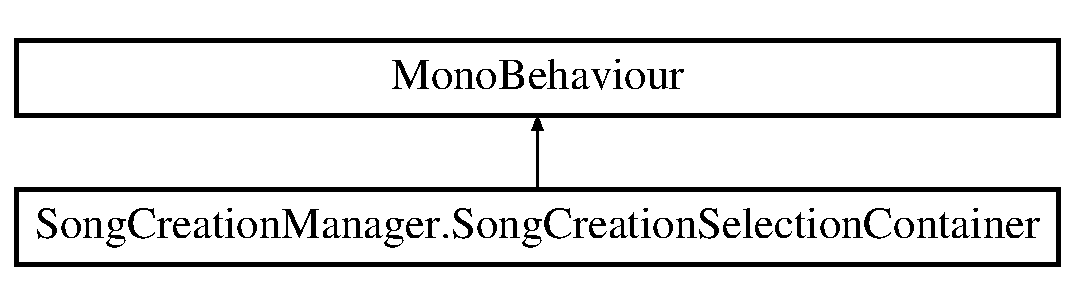
\includegraphics[height=2.000000cm]{group___s_c_m_nest_class}
\end{center}
\end{figure}
\subsubsection*{Public Member Functions}
\begin{DoxyCompactItemize}
\item 
void \hyperlink{group___s_c_m_nest_class_a29f496763424eb274f35cd29330583ac}{Set\+Container} (\hyperlink{group___s_c_m_nest_class_class_song_creation_manager_1_1_song_creation_selection_container}{Song\+Creation\+Selection\+Container} a\+Container)
\item 
void \hyperlink{group___s_c_m_nest_class_a0d65cd109a370034f580d63e823725b9}{Set\+Selected} (bool a\+Selected)
\item 
void \hyperlink{group___s_c_m_nest_class_a6477d6c5056af7998063e90e282b67ae}{On\+Selected} (bool a\+Selected)
\end{DoxyCompactItemize}
\subsubsection*{Private Member Functions}
\begin{DoxyCompactItemize}
\item 
void \hyperlink{group___s_c_m_nest_class_ae7264acac3310f5db50df38467734c06}{Awake} ()
\item 
void \hyperlink{group___s_c_m_nest_class_a26bd7667a86c8dc85429a5e4798dd30a}{Change\+Color} ()
\end{DoxyCompactItemize}
\subsubsection*{Private Attributes}
\begin{DoxyCompactItemize}
\item 
bool \hyperlink{group___s_c_m_nest_class_a1a8086defe08acc773bdc9385a9f66d2}{m\+Selected} = false
\item 
\hyperlink{group___s_c_m_nest_class_class_song_creation_manager_1_1_song_creation_selection_container}{Song\+Creation\+Selection\+Container} \hyperlink{group___s_c_m_nest_class_aae8ebcbfe18ad8706d11edac54f2da87}{m\+Container} = null
\item 
Toggle \hyperlink{group___s_c_m_nest_class_ad548c27e148377da02160715a0aca9ee}{m\+Toggle} = null
\end{DoxyCompactItemize}


\paragraph{Member Function Documentation}
\mbox{\Hypertarget{group___s_c_m_nest_class_ae7264acac3310f5db50df38467734c06}\label{group___s_c_m_nest_class_ae7264acac3310f5db50df38467734c06}} 
\index{Song\+Creation\+Manager\+::\+Song\+Creation\+Selection\+Container\+::\+Song\+Creation\+Selection\+Trigger@{Song\+Creation\+Manager\+::\+Song\+Creation\+Selection\+Container\+::\+Song\+Creation\+Selection\+Trigger}!Awake@{Awake}}
\index{Awake@{Awake}!Song\+Creation\+Manager\+::\+Song\+Creation\+Selection\+Container\+::\+Song\+Creation\+Selection\+Trigger@{Song\+Creation\+Manager\+::\+Song\+Creation\+Selection\+Container\+::\+Song\+Creation\+Selection\+Trigger}}
\subparagraph{\texorpdfstring{Awake()}{Awake()}}
{\footnotesize\ttfamily void Song\+Creation\+Manager.\+Song\+Creation\+Selection\+Container.\+Song\+Creation\+Selection\+Trigger.\+Awake (\begin{DoxyParamCaption}{ }\end{DoxyParamCaption})\hspace{0.3cm}{\ttfamily [private]}}



Definition at line 57 of file Song\+Creation\+Manager.\+cs.



References Song\+Creation\+Manager.\+Song\+Creation\+Selection\+Container.\+Song\+Creation\+Selection\+Trigger.\+On\+Selected().


\begin{DoxyCode}
58             \{
59                 \textcolor{comment}{// Get the toggle and set its listener}
60                 \hyperlink{group___s_c_m_nest_class_ad548c27e148377da02160715a0aca9ee}{mToggle} = gameObject.GetComponent<Toggle>();
61                 \hyperlink{group___s_c_m_nest_class_ad548c27e148377da02160715a0aca9ee}{mToggle}.onValueChanged.AddListener( \hyperlink{group___s_c_m_nest_class_a6477d6c5056af7998063e90e282b67ae}{OnSelected} );
62             \}
\end{DoxyCode}
\mbox{\Hypertarget{group___s_c_m_nest_class_a26bd7667a86c8dc85429a5e4798dd30a}\label{group___s_c_m_nest_class_a26bd7667a86c8dc85429a5e4798dd30a}} 
\index{Song\+Creation\+Manager\+::\+Song\+Creation\+Selection\+Container\+::\+Song\+Creation\+Selection\+Trigger@{Song\+Creation\+Manager\+::\+Song\+Creation\+Selection\+Container\+::\+Song\+Creation\+Selection\+Trigger}!Change\+Color@{Change\+Color}}
\index{Change\+Color@{Change\+Color}!Song\+Creation\+Manager\+::\+Song\+Creation\+Selection\+Container\+::\+Song\+Creation\+Selection\+Trigger@{Song\+Creation\+Manager\+::\+Song\+Creation\+Selection\+Container\+::\+Song\+Creation\+Selection\+Trigger}}
\subparagraph{\texorpdfstring{Change\+Color()}{ChangeColor()}}
{\footnotesize\ttfamily void Song\+Creation\+Manager.\+Song\+Creation\+Selection\+Container.\+Song\+Creation\+Selection\+Trigger.\+Change\+Color (\begin{DoxyParamCaption}{ }\end{DoxyParamCaption})\hspace{0.3cm}{\ttfamily [private]}}



Definition at line 93 of file Song\+Creation\+Manager.\+cs.



Referenced by Song\+Creation\+Manager.\+Song\+Creation\+Selection\+Container.\+Song\+Creation\+Selection\+Trigger.\+On\+Selected(), and Song\+Creation\+Manager.\+Song\+Creation\+Selection\+Container.\+Song\+Creation\+Selection\+Trigger.\+Set\+Selected().


\begin{DoxyCode}
94             \{
95                 \textcolor{keywordflow}{if}( \hyperlink{group___s_c_m_nest_class_a1a8086defe08acc773bdc9385a9f66d2}{mSelected} )
96                 \{
97                     \hyperlink{group___s_c_m_nest_class_ad548c27e148377da02160715a0aca9ee}{mToggle}.transform.GetChild( 0 ).GetComponent<Image>().color = \textcolor{keyword}{new} Color32( 255, 
      255, 255, 118 );
98 
99                 \}
100                 \textcolor{keywordflow}{else}
101                 \{
102                     \hyperlink{group___s_c_m_nest_class_ad548c27e148377da02160715a0aca9ee}{mToggle}.transform.GetChild( 0 ).GetComponent<Image>().color = \textcolor{keyword}{new} Color32( 255, 
      255, 255, 255 );
103                 \}
104             \}
\end{DoxyCode}
\mbox{\Hypertarget{group___s_c_m_nest_class_a6477d6c5056af7998063e90e282b67ae}\label{group___s_c_m_nest_class_a6477d6c5056af7998063e90e282b67ae}} 
\index{Song\+Creation\+Manager\+::\+Song\+Creation\+Selection\+Container\+::\+Song\+Creation\+Selection\+Trigger@{Song\+Creation\+Manager\+::\+Song\+Creation\+Selection\+Container\+::\+Song\+Creation\+Selection\+Trigger}!On\+Selected@{On\+Selected}}
\index{On\+Selected@{On\+Selected}!Song\+Creation\+Manager\+::\+Song\+Creation\+Selection\+Container\+::\+Song\+Creation\+Selection\+Trigger@{Song\+Creation\+Manager\+::\+Song\+Creation\+Selection\+Container\+::\+Song\+Creation\+Selection\+Trigger}}
\subparagraph{\texorpdfstring{On\+Selected()}{OnSelected()}}
{\footnotesize\ttfamily void Song\+Creation\+Manager.\+Song\+Creation\+Selection\+Container.\+Song\+Creation\+Selection\+Trigger.\+On\+Selected (\begin{DoxyParamCaption}\item[{bool}]{a\+Selected }\end{DoxyParamCaption})}



Definition at line 111 of file Song\+Creation\+Manager.\+cs.



References Song\+Creation\+Manager.\+Song\+Creation\+Selection\+Container.\+Song\+Creation\+Selection\+Trigger.\+Change\+Color(), and Song\+Creation\+Manager.\+Song\+Creation\+Selection\+Container.\+Handle\+Toggle().



Referenced by Song\+Creation\+Manager.\+Song\+Creation\+Selection\+Container.\+Song\+Creation\+Selection\+Trigger.\+Awake(), and Song\+Creation\+Manager.\+Song\+Creation\+Selection\+Container.\+Song\+Creation\+Selection\+Trigger.\+Set\+Selected().


\begin{DoxyCode}
112             \{
113                 \textcolor{comment}{// If this object is now selected, then change the color and send it to the handler.}
114                 \textcolor{keywordflow}{if}( aSelected )
115                 \{
116                     \hyperlink{group___s_c_m_nest_class_a1a8086defe08acc773bdc9385a9f66d2}{mSelected} = aSelected;
117                     \hyperlink{group___s_c_m_nest_class_a26bd7667a86c8dc85429a5e4798dd30a}{ChangeColor}();
118                     \hyperlink{group___s_c_m_nest_class_aae8ebcbfe18ad8706d11edac54f2da87}{mContainer}.\hyperlink{group___s_c_m_nest_class_a534fec983fb7e5a7f948513672aa64b4}{HandleToggle}( \textcolor{keyword}{this} );
119                 \}
120                 \textcolor{comment}{// This object can not be unselected by clicking on it. Set the value back to selected.}
121                 \textcolor{keywordflow}{else}
122                 \{
123                     \hyperlink{group___s_c_m_nest_class_ad548c27e148377da02160715a0aca9ee}{mToggle}.onValueChanged.RemoveListener( \hyperlink{group___s_c_m_nest_class_a6477d6c5056af7998063e90e282b67ae}{OnSelected} );
124                     \hyperlink{group___s_c_m_nest_class_ad548c27e148377da02160715a0aca9ee}{mToggle}.isOn = \textcolor{keyword}{true};
125                     \hyperlink{group___s_c_m_nest_class_ad548c27e148377da02160715a0aca9ee}{mToggle}.onValueChanged.AddListener( \hyperlink{group___s_c_m_nest_class_a6477d6c5056af7998063e90e282b67ae}{OnSelected} );
126                 \}
127 
128             \}
\end{DoxyCode}
\mbox{\Hypertarget{group___s_c_m_nest_class_a29f496763424eb274f35cd29330583ac}\label{group___s_c_m_nest_class_a29f496763424eb274f35cd29330583ac}} 
\index{Song\+Creation\+Manager\+::\+Song\+Creation\+Selection\+Container\+::\+Song\+Creation\+Selection\+Trigger@{Song\+Creation\+Manager\+::\+Song\+Creation\+Selection\+Container\+::\+Song\+Creation\+Selection\+Trigger}!Set\+Container@{Set\+Container}}
\index{Set\+Container@{Set\+Container}!Song\+Creation\+Manager\+::\+Song\+Creation\+Selection\+Container\+::\+Song\+Creation\+Selection\+Trigger@{Song\+Creation\+Manager\+::\+Song\+Creation\+Selection\+Container\+::\+Song\+Creation\+Selection\+Trigger}}
\subparagraph{\texorpdfstring{Set\+Container()}{SetContainer()}}
{\footnotesize\ttfamily void Song\+Creation\+Manager.\+Song\+Creation\+Selection\+Container.\+Song\+Creation\+Selection\+Trigger.\+Set\+Container (\begin{DoxyParamCaption}\item[{\hyperlink{group___s_c_m_nest_class_class_song_creation_manager_1_1_song_creation_selection_container}{Song\+Creation\+Selection\+Container}}]{a\+Container }\end{DoxyParamCaption})}



Definition at line 69 of file Song\+Creation\+Manager.\+cs.



Referenced by Song\+Creation\+Manager.\+Song\+Creation\+Selection\+Container.\+Awake().


\begin{DoxyCode}
70             \{
71                 \hyperlink{group___s_c_m_nest_class_aae8ebcbfe18ad8706d11edac54f2da87}{mContainer} = aContainer;
72             \}
\end{DoxyCode}
\mbox{\Hypertarget{group___s_c_m_nest_class_a0d65cd109a370034f580d63e823725b9}\label{group___s_c_m_nest_class_a0d65cd109a370034f580d63e823725b9}} 
\index{Song\+Creation\+Manager\+::\+Song\+Creation\+Selection\+Container\+::\+Song\+Creation\+Selection\+Trigger@{Song\+Creation\+Manager\+::\+Song\+Creation\+Selection\+Container\+::\+Song\+Creation\+Selection\+Trigger}!Set\+Selected@{Set\+Selected}}
\index{Set\+Selected@{Set\+Selected}!Song\+Creation\+Manager\+::\+Song\+Creation\+Selection\+Container\+::\+Song\+Creation\+Selection\+Trigger@{Song\+Creation\+Manager\+::\+Song\+Creation\+Selection\+Container\+::\+Song\+Creation\+Selection\+Trigger}}
\subparagraph{\texorpdfstring{Set\+Selected()}{SetSelected()}}
{\footnotesize\ttfamily void Song\+Creation\+Manager.\+Song\+Creation\+Selection\+Container.\+Song\+Creation\+Selection\+Trigger.\+Set\+Selected (\begin{DoxyParamCaption}\item[{bool}]{a\+Selected }\end{DoxyParamCaption})}



Definition at line 75 of file Song\+Creation\+Manager.\+cs.



References Song\+Creation\+Manager.\+Song\+Creation\+Selection\+Container.\+Song\+Creation\+Selection\+Trigger.\+Change\+Color(), and Song\+Creation\+Manager.\+Song\+Creation\+Selection\+Container.\+Song\+Creation\+Selection\+Trigger.\+On\+Selected().



Referenced by Song\+Creation\+Manager.\+Song\+Creation\+Selection\+Container.\+Awake(), Song\+Creation\+Manager.\+Song\+Creation\+Selection\+Container.\+Handle\+Toggle(), and Song\+Creation\+Manager.\+Song\+Creation\+Selection\+Container.\+Set\+Selected().


\begin{DoxyCode}
76             \{
77                 \hyperlink{group___s_c_m_nest_class_a1a8086defe08acc773bdc9385a9f66d2}{mSelected} = aSelected;
78 
79                 \textcolor{comment}{// Change the color to indicate that this is or isn't the selected object}
80                 \hyperlink{group___s_c_m_nest_class_a26bd7667a86c8dc85429a5e4798dd30a}{ChangeColor}();
81 
82                 \textcolor{comment}{// Set the value of the toggle.}
83                 \hyperlink{group___s_c_m_nest_class_ad548c27e148377da02160715a0aca9ee}{mToggle}.onValueChanged.RemoveListener( \hyperlink{group___s_c_m_nest_class_a6477d6c5056af7998063e90e282b67ae}{OnSelected} );
84                 \hyperlink{group___s_c_m_nest_class_ad548c27e148377da02160715a0aca9ee}{mToggle}.isOn = aSelected;
85                 \hyperlink{group___s_c_m_nest_class_ad548c27e148377da02160715a0aca9ee}{mToggle}.onValueChanged.AddListener( \hyperlink{group___s_c_m_nest_class_a6477d6c5056af7998063e90e282b67ae}{OnSelected} );
86             \}
\end{DoxyCode}


\paragraph{Member Data Documentation}
\mbox{\Hypertarget{group___s_c_m_nest_class_aae8ebcbfe18ad8706d11edac54f2da87}\label{group___s_c_m_nest_class_aae8ebcbfe18ad8706d11edac54f2da87}} 
\index{Song\+Creation\+Manager\+::\+Song\+Creation\+Selection\+Container\+::\+Song\+Creation\+Selection\+Trigger@{Song\+Creation\+Manager\+::\+Song\+Creation\+Selection\+Container\+::\+Song\+Creation\+Selection\+Trigger}!m\+Container@{m\+Container}}
\index{m\+Container@{m\+Container}!Song\+Creation\+Manager\+::\+Song\+Creation\+Selection\+Container\+::\+Song\+Creation\+Selection\+Trigger@{Song\+Creation\+Manager\+::\+Song\+Creation\+Selection\+Container\+::\+Song\+Creation\+Selection\+Trigger}}
\subparagraph{\texorpdfstring{m\+Container}{mContainer}}
{\footnotesize\ttfamily \hyperlink{group___s_c_m_nest_class_class_song_creation_manager_1_1_song_creation_selection_container}{Song\+Creation\+Selection\+Container} Song\+Creation\+Manager.\+Song\+Creation\+Selection\+Container.\+Song\+Creation\+Selection\+Trigger.\+m\+Container = null\hspace{0.3cm}{\ttfamily [private]}}



Definition at line 51 of file Song\+Creation\+Manager.\+cs.

\mbox{\Hypertarget{group___s_c_m_nest_class_a1a8086defe08acc773bdc9385a9f66d2}\label{group___s_c_m_nest_class_a1a8086defe08acc773bdc9385a9f66d2}} 
\index{Song\+Creation\+Manager\+::\+Song\+Creation\+Selection\+Container\+::\+Song\+Creation\+Selection\+Trigger@{Song\+Creation\+Manager\+::\+Song\+Creation\+Selection\+Container\+::\+Song\+Creation\+Selection\+Trigger}!m\+Selected@{m\+Selected}}
\index{m\+Selected@{m\+Selected}!Song\+Creation\+Manager\+::\+Song\+Creation\+Selection\+Container\+::\+Song\+Creation\+Selection\+Trigger@{Song\+Creation\+Manager\+::\+Song\+Creation\+Selection\+Container\+::\+Song\+Creation\+Selection\+Trigger}}
\subparagraph{\texorpdfstring{m\+Selected}{mSelected}}
{\footnotesize\ttfamily bool Song\+Creation\+Manager.\+Song\+Creation\+Selection\+Container.\+Song\+Creation\+Selection\+Trigger.\+m\+Selected = false\hspace{0.3cm}{\ttfamily [private]}}



Definition at line 50 of file Song\+Creation\+Manager.\+cs.

\mbox{\Hypertarget{group___s_c_m_nest_class_ad548c27e148377da02160715a0aca9ee}\label{group___s_c_m_nest_class_ad548c27e148377da02160715a0aca9ee}} 
\index{Song\+Creation\+Manager\+::\+Song\+Creation\+Selection\+Container\+::\+Song\+Creation\+Selection\+Trigger@{Song\+Creation\+Manager\+::\+Song\+Creation\+Selection\+Container\+::\+Song\+Creation\+Selection\+Trigger}!m\+Toggle@{m\+Toggle}}
\index{m\+Toggle@{m\+Toggle}!Song\+Creation\+Manager\+::\+Song\+Creation\+Selection\+Container\+::\+Song\+Creation\+Selection\+Trigger@{Song\+Creation\+Manager\+::\+Song\+Creation\+Selection\+Container\+::\+Song\+Creation\+Selection\+Trigger}}
\subparagraph{\texorpdfstring{m\+Toggle}{mToggle}}
{\footnotesize\ttfamily Toggle Song\+Creation\+Manager.\+Song\+Creation\+Selection\+Container.\+Song\+Creation\+Selection\+Trigger.\+m\+Toggle = null\hspace{0.3cm}{\ttfamily [private]}}



Definition at line 52 of file Song\+Creation\+Manager.\+cs.

\index{Song\+Creation\+Manager\+::\+Song\+Creation\+Selection\+Container@{Song\+Creation\+Manager\+::\+Song\+Creation\+Selection\+Container}}\label{class_song_creation_manager_1_1_song_creation_selection_container}
\Hypertarget{group___s_c_m_nest_class_class_song_creation_manager_1_1_song_creation_selection_container}
\subsubsection{class Song\+Creation\+Manager\+:\+:Song\+Creation\+Selection\+Container}


Definition at line 40 of file Song\+Creation\+Manager.\+cs.

Inheritance diagram for Song\+Creation\+Manager.\+Song\+Creation\+Selection\+Container\+:\begin{figure}[H]
\begin{center}
\leavevmode
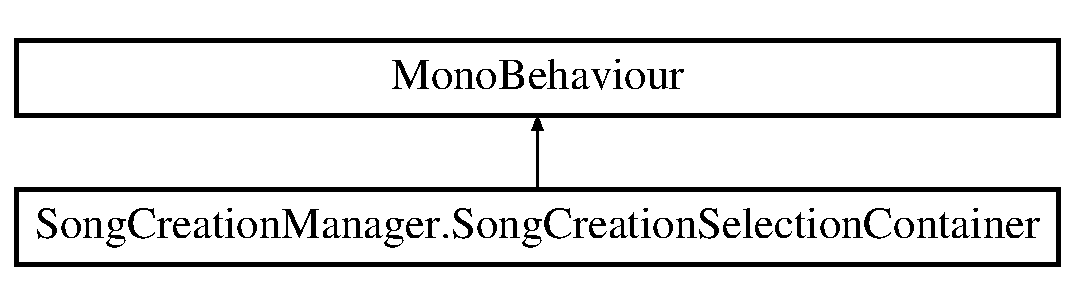
\includegraphics[height=2.000000cm]{group___s_c_m_nest_class}
\end{center}
\end{figure}
\subsubsection*{Public Member Functions}
\begin{DoxyCompactItemize}
\item 
\hyperlink{group___music_enums_gaf11b5f079adbb21c800b9eca1c5c3cbd}{Music.\+N\+O\+T\+E\+\_\+\+L\+E\+N\+G\+TH} \hyperlink{group___s_c_m_nest_class_ae73f2b2c2f567ecaf6ce10f85c30956a}{Get\+Selected} ()
\item 
void \hyperlink{group___s_c_m_nest_class_ab3d74be007528e4e6686f89e8e993b3b}{Set\+Selected} (\hyperlink{group___music_enums_gaf11b5f079adbb21c800b9eca1c5c3cbd}{Music.\+N\+O\+T\+E\+\_\+\+L\+E\+N\+G\+TH} a\+Selection)
\end{DoxyCompactItemize}
\subsubsection*{Private Member Functions}
\begin{DoxyCompactItemize}
\item 
void \hyperlink{group___s_c_m_nest_class_a786a838268b7102ae38c546100c3e6ac}{Awake} ()
\item 
void \hyperlink{group___s_c_m_nest_class_a534fec983fb7e5a7f948513672aa64b4}{Handle\+Toggle} (\hyperlink{group___s_c_m_nest_class_class_song_creation_manager_1_1_song_creation_selection_container_1_1_song_creation_selection_trigger}{Song\+Creation\+Selection\+Trigger} a\+Trigger)
\end{DoxyCompactItemize}
\subsubsection*{Private Attributes}
\begin{DoxyCompactItemize}
\item 
int \hyperlink{group___s_c_m_nest_class_a1684b25b3eb0e87f189996de22bf9792}{m\+Selected\+Index} = 0
\item 
\hyperlink{group___s_c_m_nest_class_class_song_creation_manager_1_1_song_creation_selection_container_1_1_song_creation_selection_trigger}{Song\+Creation\+Selection\+Trigger} \mbox{[}$\,$\mbox{]} \hyperlink{group___s_c_m_nest_class_aeda161975a8a683281b9388b2c905ae8}{m\+Triggers} = null
\end{DoxyCompactItemize}


\paragraph{Member Function Documentation}
\mbox{\Hypertarget{group___s_c_m_nest_class_a786a838268b7102ae38c546100c3e6ac}\label{group___s_c_m_nest_class_a786a838268b7102ae38c546100c3e6ac}} 
\index{Song\+Creation\+Manager\+::\+Song\+Creation\+Selection\+Container@{Song\+Creation\+Manager\+::\+Song\+Creation\+Selection\+Container}!Awake@{Awake}}
\index{Awake@{Awake}!Song\+Creation\+Manager\+::\+Song\+Creation\+Selection\+Container@{Song\+Creation\+Manager\+::\+Song\+Creation\+Selection\+Container}}
\subparagraph{\texorpdfstring{Awake()}{Awake()}}
{\footnotesize\ttfamily void Song\+Creation\+Manager.\+Song\+Creation\+Selection\+Container.\+Awake (\begin{DoxyParamCaption}{ }\end{DoxyParamCaption})\hspace{0.3cm}{\ttfamily [private]}}



Definition at line 141 of file Song\+Creation\+Manager.\+cs.



References Song\+Creation\+Manager.\+Song\+Creation\+Selection\+Container.\+Song\+Creation\+Selection\+Trigger.\+Set\+Container(), and Song\+Creation\+Manager.\+Song\+Creation\+Selection\+Container.\+Song\+Creation\+Selection\+Trigger.\+Set\+Selected().


\begin{DoxyCode}
142         \{
143             \textcolor{comment}{// Set up the triggers.}
144             \hyperlink{group___s_c_m_nest_class_aeda161975a8a683281b9388b2c905ae8}{mTriggers} = \textcolor{keyword}{new} SongCreationSelectionTrigger[13];
145             \textcolor{keywordflow}{for}( \textcolor{keywordtype}{int} i = 0; i < 13; i++ )
146             \{
147                 \hyperlink{group___s_c_m_nest_class_aeda161975a8a683281b9388b2c905ae8}{mTriggers}[i] = gameObject.transform.GetChild( i + 1 ).gameObject.AddComponent<
      SongCreationSelectionTrigger>();
148                 \hyperlink{group___s_c_m_nest_class_aeda161975a8a683281b9388b2c905ae8}{mTriggers}[i].\hyperlink{group___s_c_m_nest_class_a29f496763424eb274f35cd29330583ac}{SetContainer}( \textcolor{keyword}{this} );
149                 \hyperlink{group___s_c_m_nest_class_aeda161975a8a683281b9388b2c905ae8}{mTriggers}[i].\hyperlink{group___s_c_m_nest_class_a0d65cd109a370034f580d63e823725b9}{SetSelected}( \textcolor{keyword}{false} );
150             \}
151 
152             \textcolor{comment}{// Set the default selection (Quarter note).}
153             \hyperlink{group___s_c_m_nest_class_aeda161975a8a683281b9388b2c905ae8}{mTriggers}[12].\hyperlink{group___s_c_m_nest_class_a0d65cd109a370034f580d63e823725b9}{SetSelected}( \textcolor{keyword}{true} );
154             \hyperlink{group___s_c_m_nest_class_a1684b25b3eb0e87f189996de22bf9792}{mSelectedIndex} = 12;
155         \}
\end{DoxyCode}
\mbox{\Hypertarget{group___s_c_m_nest_class_ae73f2b2c2f567ecaf6ce10f85c30956a}\label{group___s_c_m_nest_class_ae73f2b2c2f567ecaf6ce10f85c30956a}} 
\index{Song\+Creation\+Manager\+::\+Song\+Creation\+Selection\+Container@{Song\+Creation\+Manager\+::\+Song\+Creation\+Selection\+Container}!Get\+Selected@{Get\+Selected}}
\index{Get\+Selected@{Get\+Selected}!Song\+Creation\+Manager\+::\+Song\+Creation\+Selection\+Container@{Song\+Creation\+Manager\+::\+Song\+Creation\+Selection\+Container}}
\subparagraph{\texorpdfstring{Get\+Selected()}{GetSelected()}}
{\footnotesize\ttfamily \hyperlink{group___music_enums_gaf11b5f079adbb21c800b9eca1c5c3cbd}{Music.\+N\+O\+T\+E\+\_\+\+L\+E\+N\+G\+TH} Song\+Creation\+Manager.\+Song\+Creation\+Selection\+Container.\+Get\+Selected (\begin{DoxyParamCaption}{ }\end{DoxyParamCaption})}



Definition at line 162 of file Song\+Creation\+Manager.\+cs.



References Song\+Creation\+Manager.\+Song\+Creation\+Selection\+Container.\+m\+Selected\+Index.



Referenced by Song\+Creation\+Manager.\+On\+Create\+Note(), and Song\+Creation\+Manager.\+On\+Modify\+Note().


\begin{DoxyCode}
163         \{
164             \textcolor{keywordflow}{return} (\hyperlink{class_music}{Music}.\hyperlink{group___music_enums_gaf11b5f079adbb21c800b9eca1c5c3cbd}{NOTE\_LENGTH})\hyperlink{group___s_c_m_nest_class_a1684b25b3eb0e87f189996de22bf9792}{mSelectedIndex};
165         \}
\end{DoxyCode}
\mbox{\Hypertarget{group___s_c_m_nest_class_a534fec983fb7e5a7f948513672aa64b4}\label{group___s_c_m_nest_class_a534fec983fb7e5a7f948513672aa64b4}} 
\index{Song\+Creation\+Manager\+::\+Song\+Creation\+Selection\+Container@{Song\+Creation\+Manager\+::\+Song\+Creation\+Selection\+Container}!Handle\+Toggle@{Handle\+Toggle}}
\index{Handle\+Toggle@{Handle\+Toggle}!Song\+Creation\+Manager\+::\+Song\+Creation\+Selection\+Container@{Song\+Creation\+Manager\+::\+Song\+Creation\+Selection\+Container}}
\subparagraph{\texorpdfstring{Handle\+Toggle()}{HandleToggle()}}
{\footnotesize\ttfamily void Song\+Creation\+Manager.\+Song\+Creation\+Selection\+Container.\+Handle\+Toggle (\begin{DoxyParamCaption}\item[{\hyperlink{group___s_c_m_nest_class_class_song_creation_manager_1_1_song_creation_selection_container_1_1_song_creation_selection_trigger}{Song\+Creation\+Selection\+Trigger}}]{a\+Trigger }\end{DoxyParamCaption})\hspace{0.3cm}{\ttfamily [private]}}



Definition at line 193 of file Song\+Creation\+Manager.\+cs.



References Song\+Creation\+Manager.\+Song\+Creation\+Selection\+Container.\+Song\+Creation\+Selection\+Trigger.\+Set\+Selected().



Referenced by Song\+Creation\+Manager.\+Song\+Creation\+Selection\+Container.\+Song\+Creation\+Selection\+Trigger.\+On\+Selected().


\begin{DoxyCode}
194         \{
195             \textcolor{comment}{// Set all other triggers to unselected.}
196             \textcolor{keywordflow}{for}( \textcolor{keywordtype}{int} i = 0; i < 13; i++ )
197             \{
198                 \textcolor{keywordflow}{if}( \hyperlink{group___s_c_m_nest_class_aeda161975a8a683281b9388b2c905ae8}{mTriggers}[i] != aTrigger )
199                 \{
200                     \hyperlink{group___s_c_m_nest_class_aeda161975a8a683281b9388b2c905ae8}{mTriggers}[i].\hyperlink{group___s_c_m_nest_class_a0d65cd109a370034f580d63e823725b9}{SetSelected}( \textcolor{keyword}{false} );
201                 \}
202 
203                 \textcolor{comment}{// Update the current selection.}
204                 \textcolor{keywordflow}{else}
205                 \{
206                     \hyperlink{group___s_c_m_nest_class_a1684b25b3eb0e87f189996de22bf9792}{mSelectedIndex} = i;
207                 \}
208             \}
209         \}
\end{DoxyCode}
\mbox{\Hypertarget{group___s_c_m_nest_class_ab3d74be007528e4e6686f89e8e993b3b}\label{group___s_c_m_nest_class_ab3d74be007528e4e6686f89e8e993b3b}} 
\index{Song\+Creation\+Manager\+::\+Song\+Creation\+Selection\+Container@{Song\+Creation\+Manager\+::\+Song\+Creation\+Selection\+Container}!Set\+Selected@{Set\+Selected}}
\index{Set\+Selected@{Set\+Selected}!Song\+Creation\+Manager\+::\+Song\+Creation\+Selection\+Container@{Song\+Creation\+Manager\+::\+Song\+Creation\+Selection\+Container}}
\subparagraph{\texorpdfstring{Set\+Selected()}{SetSelected()}}
{\footnotesize\ttfamily void Song\+Creation\+Manager.\+Song\+Creation\+Selection\+Container.\+Set\+Selected (\begin{DoxyParamCaption}\item[{\hyperlink{group___music_enums_gaf11b5f079adbb21c800b9eca1c5c3cbd}{Music.\+N\+O\+T\+E\+\_\+\+L\+E\+N\+G\+TH}}]{a\+Selection }\end{DoxyParamCaption})}



Definition at line 168 of file Song\+Creation\+Manager.\+cs.



References Song\+Creation\+Manager.\+Song\+Creation\+Selection\+Container.\+Song\+Creation\+Selection\+Trigger.\+Set\+Selected().



Referenced by Song\+Creation\+Manager.\+Awake(), Song\+Creation\+Manager.\+On\+Create\+Note(), and Song\+Creation\+Manager.\+On\+Edit\+Event().


\begin{DoxyCode}
169         \{
170             \textcolor{comment}{// Update the private variable.}
171             \hyperlink{group___s_c_m_nest_class_a1684b25b3eb0e87f189996de22bf9792}{mSelectedIndex} = (int)aSelection;
172 
173             \textcolor{comment}{// Update the child objects.}
174             \textcolor{keywordflow}{for}( \textcolor{keywordtype}{int} i = 0; i < 13; i++ )
175             \{
176                 \textcolor{keywordflow}{if}( i != \hyperlink{group___s_c_m_nest_class_a1684b25b3eb0e87f189996de22bf9792}{mSelectedIndex} )
177                 \{
178                     \hyperlink{group___s_c_m_nest_class_aeda161975a8a683281b9388b2c905ae8}{mTriggers}[i].\hyperlink{group___s_c_m_nest_class_a0d65cd109a370034f580d63e823725b9}{SetSelected}( \textcolor{keyword}{false} );
179                 \}
180                 \textcolor{keywordflow}{else}
181                 \{
182                     \hyperlink{group___s_c_m_nest_class_aeda161975a8a683281b9388b2c905ae8}{mTriggers}[i].\hyperlink{group___s_c_m_nest_class_a0d65cd109a370034f580d63e823725b9}{SetSelected}( \textcolor{keyword}{true} );
183                 \}
184             \}
185         \}
\end{DoxyCode}


\paragraph{Member Data Documentation}
\mbox{\Hypertarget{group___s_c_m_nest_class_a1684b25b3eb0e87f189996de22bf9792}\label{group___s_c_m_nest_class_a1684b25b3eb0e87f189996de22bf9792}} 
\index{Song\+Creation\+Manager\+::\+Song\+Creation\+Selection\+Container@{Song\+Creation\+Manager\+::\+Song\+Creation\+Selection\+Container}!m\+Selected\+Index@{m\+Selected\+Index}}
\index{m\+Selected\+Index@{m\+Selected\+Index}!Song\+Creation\+Manager\+::\+Song\+Creation\+Selection\+Container@{Song\+Creation\+Manager\+::\+Song\+Creation\+Selection\+Container}}
\subparagraph{\texorpdfstring{m\+Selected\+Index}{mSelectedIndex}}
{\footnotesize\ttfamily int Song\+Creation\+Manager.\+Song\+Creation\+Selection\+Container.\+m\+Selected\+Index = 0\hspace{0.3cm}{\ttfamily [private]}}



Definition at line 134 of file Song\+Creation\+Manager.\+cs.



Referenced by Song\+Creation\+Manager.\+Song\+Creation\+Selection\+Container.\+Get\+Selected().

\mbox{\Hypertarget{group___s_c_m_nest_class_aeda161975a8a683281b9388b2c905ae8}\label{group___s_c_m_nest_class_aeda161975a8a683281b9388b2c905ae8}} 
\index{Song\+Creation\+Manager\+::\+Song\+Creation\+Selection\+Container@{Song\+Creation\+Manager\+::\+Song\+Creation\+Selection\+Container}!m\+Triggers@{m\+Triggers}}
\index{m\+Triggers@{m\+Triggers}!Song\+Creation\+Manager\+::\+Song\+Creation\+Selection\+Container@{Song\+Creation\+Manager\+::\+Song\+Creation\+Selection\+Container}}
\subparagraph{\texorpdfstring{m\+Triggers}{mTriggers}}
{\footnotesize\ttfamily \hyperlink{group___s_c_m_nest_class_class_song_creation_manager_1_1_song_creation_selection_container_1_1_song_creation_selection_trigger}{Song\+Creation\+Selection\+Trigger} \mbox{[}$\,$\mbox{]} Song\+Creation\+Manager.\+Song\+Creation\+Selection\+Container.\+m\+Triggers = null\hspace{0.3cm}{\ttfamily [private]}}



Definition at line 135 of file Song\+Creation\+Manager.\+cs.


\hypertarget{group___doc_s_c___n_d}{}\section{Note Display}
\label{group___doc_s_c___n_d}\index{Note Display@{Note Display}}


Modules for displaying the \hyperlink{group___music_structs_struct_music_1_1_combined_note}{notes} in the \hyperlink{class_song}{Song} being created.  


\subsection*{Modules}
\begin{DoxyCompactItemize}
\item 
\hyperlink{group___doc_s_c___m_d_p}{Measure Display Panel}
\begin{DoxyCompactList}\small\item\em Class that handles a specific measure of the \hyperlink{class_song}{Song} that is being created. \end{DoxyCompactList}\item 
\hyperlink{group___doc_s_c___n_d_c}{Note Display Container}
\begin{DoxyCompactList}\small\item\em Connects the \hyperlink{class_s_c___measure_display_panel}{S\+C\+\_\+\+Measure\+Display\+Panel} objects to the \hyperlink{group___doc_s_c}{Song Creation Interface} and provides handling for them. \end{DoxyCompactList}\item 
\hyperlink{group___doc_s_c___n_d_p}{Note Display Panel}
\begin{DoxyCompactList}\small\item\em Class that displays a specific \hyperlink{group___music_structs_struct_music_1_1_combined_note}{note} of the \hyperlink{class_song}{Song} that is being created. \end{DoxyCompactList}\end{DoxyCompactItemize}


\subsection{Detailed Description}
Modules for displaying the \hyperlink{group___music_structs_struct_music_1_1_combined_note}{notes} in the \hyperlink{class_song}{Song} being created. 


\hypertarget{group___doc_s_c___n_d_c}{}\section{Note Display Container}
\label{group___doc_s_c___n_d_c}\index{Note Display Container@{Note Display Container}}


Connects the \hyperlink{class_s_c___measure_display_panel}{S\+C\+\_\+\+Measure\+Display\+Panel} objects to the \hyperlink{group___doc_s_c}{Song Creation Interface} and provides handling for them.  


\subsection*{Modules}
\begin{DoxyCompactItemize}
\item 
\hyperlink{group___s_c___n_d_c_const}{Constants}
\item 
\hyperlink{group___s_c___n_d_c_handlers}{Event Handlers}
\item 
\hyperlink{group___s_c___n_d_c_priv_var}{Private Variables}
\item 
\hyperlink{group___s_c___n_d_c_pub_func}{Public Functions}
\item 
\hyperlink{group___s_c___n_d_c_unity}{Unity Functions}
\end{DoxyCompactItemize}


\subsection{Detailed Description}
Connects the \hyperlink{class_s_c___measure_display_panel}{S\+C\+\_\+\+Measure\+Display\+Panel} objects to the \hyperlink{group___doc_s_c}{Song Creation Interface} and provides handling for them. 

\hypertarget{group___doc_s_c___n_d_c_DocSC_NDCInfo}{}\subsection{Information}\label{group___doc_s_c___n_d_c_DocSC_NDCInfo}
\hypertarget{group___doc_s_c___n_d_c_DocSC_NDCConst}{}\subsection{Constants}\label{group___doc_s_c___n_d_c_DocSC_NDCConst}
Constants used by the \hyperlink{class_s_c___note_display_container}{S\+C\+\_\+\+Note\+Display\+Container}. ~\newline
 \hyperlink{group___s_c___n_d_c_const}{More details}.\hypertarget{group___doc_s_c___n_d_c_DocSC_NDCPrivVar}{}\subsection{Private Variables}\label{group___doc_s_c___n_d_c_DocSC_NDCPrivVar}
Variables used internally by the \hyperlink{class_s_c___note_display_container}{S\+C\+\_\+\+Note\+Display\+Container}. ~\newline
 \hyperlink{group___s_c___n_d_c_priv_var}{More details}.\hypertarget{group___doc_s_c___n_d_c_DocSC_NDCUnity}{}\subsection{Unity Functions}\label{group___doc_s_c___n_d_c_DocSC_NDCUnity}
Functions called automatically by Unity. ~\newline
 \hyperlink{group___s_c___n_d_c_unity}{More details}.\hypertarget{group___doc_s_c___n_d_c_DocSC_NDCPubFunc}{}\subsection{Public Functions}\label{group___doc_s_c___n_d_c_DocSC_NDCPubFunc}
Functions for other classes to interact with the \hyperlink{class_s_c___note_display_container}{S\+C\+\_\+\+Note\+Display\+Container}. ~\newline
 \hyperlink{group___s_c___n_d_c_pub_func}{More details}.\hypertarget{group___doc_s_c___n_d_c_DocSC_NDCHandlers}{}\subsection{Event Handlers}\label{group___doc_s_c___n_d_c_DocSC_NDCHandlers}
Functions that are called by the \hyperlink{class_s_c___note_display_container}{S\+C\+\_\+\+Note\+Display\+Container} to handle events. ~\newline
 \hyperlink{group___s_c___n_d_c_handlers}{More details}.\hypertarget{group___doc_s_c___n_d_c_DocSC_NDCCode}{}\subsection{Code}\label{group___doc_s_c___n_d_c_DocSC_NDCCode}

\begin{DoxyCodeInclude}
1 \textcolor{keyword}{using} \hyperlink{namespace_system}{System}.Collections;
2 \textcolor{keyword}{using} \hyperlink{namespace_system}{System}.Collections.Generic;
3 \textcolor{keyword}{using} \hyperlink{namespace_unity_engine}{UnityEngine};
4 \textcolor{keyword}{using} \hyperlink{namespace_unity_engine}{UnityEngine}.Assertions;
5 \textcolor{keyword}{using} \hyperlink{namespace_unity_engine}{UnityEngine}.EventSystems;
6 \textcolor{keyword}{using} \hyperlink{namespace_unity_engine}{UnityEngine}.SceneManagement;
7 \textcolor{keyword}{using} \hyperlink{namespace_unity_engine}{UnityEngine}.UI;
8 \textcolor{comment}{}
9 \textcolor{comment}{/**}
10 \textcolor{comment}{ * @class SC\_NoteDisplayContainer}
11 \textcolor{comment}{ * @brief Connects the SC\_MeasureDisplayPanel objects to the @link DocSC Song Creation Interface@endlink
       and provides handling for them.}
12 \textcolor{comment}{*/}
13 \textcolor{keyword}{public} \textcolor{keyword}{class }\hyperlink{class_s_c___note_display_container}{SC\_NoteDisplayContainer} : MonoBehaviour
14 \{
15     \textcolor{comment}{/*************************************************************************/}\textcolor{comment}{/** }
16 \textcolor{comment}{    * @defgroup SC\_NDCConst Constants}
17 \textcolor{comment}{    * @ingroup DocSC\_NDC}
18 \textcolor{comment}{    * Constants used by the SC\_NoteDisplayContainer.}
19 \textcolor{comment}{    * @\{}
20 \textcolor{comment}{    *****************************************************************************/}
21     \textcolor{keyword}{private} \textcolor{keyword}{const} \textcolor{keywordtype}{string} MEASURE\_PANEL\_PREFAB\_PATH = \textcolor{stringliteral}{"Audio/Prefabs/SongCreation/MeasurePanelPrefab"}; \textcolor{comment}{//!<
       The path to load the prefab for the @link DocSC\_MDP measure display panel objects@endlink.}
22 \textcolor{comment}{}
23     \textcolor{comment}{/*************************************************************************/}\textcolor{comment}{/** }
24 \textcolor{comment}{    * @\}}
25 \textcolor{comment}{    * @defgroup SC\_NDCPrivVar Private Variables}
26 \textcolor{comment}{    * @ingroup DocSC\_NDC}
27 \textcolor{comment}{    * Variables used internally by the SC\_NoteDisplayContainer.}
28 \textcolor{comment}{    * @\{}
29 \textcolor{comment}{    *****************************************************************************/}
30     \textcolor{keyword}{private} \textcolor{keywordtype}{int} mNumNotes = 0; \textcolor{comment}{//!< The number of overall @link Music::CombinedNote notes@endlink in the
       container.}
31 \textcolor{comment}{}    \textcolor{keyword}{private} \textcolor{keywordtype}{int} mCurrentMeasure = -1; \textcolor{comment}{//!< The current @link DocSC\_MDP measure@endlink.}
32 \textcolor{comment}{}    \textcolor{keyword}{private} List<SC\_MeasureDisplayPanel> mMeasures = null; \textcolor{comment}{//!< The @link DocSC\_MDP measures@endlink in the
       container.}
33 \textcolor{comment}{}    \textcolor{keyword}{private} Sprite[] mSprites = null; \textcolor{comment}{//!< The images to show the @link Music::MelodyNote.Length note
       lengths@endlink and @link Music::CombinedNote.OffsetFromPrevNote offsets@endlink.}
34 \textcolor{comment}{}
35     \textcolor{comment}{/*************************************************************************/}\textcolor{comment}{/** }
36 \textcolor{comment}{    * @\}}
37 \textcolor{comment}{    * @defgroup SC\_NDCUnity Unity Functions}
38 \textcolor{comment}{    * @ingroup DocSC\_NDC}
39 \textcolor{comment}{    * Functions called automatically by Unity.}
40 \textcolor{comment}{    * @\{}
41 \textcolor{comment}{    *****************************************************************************/}
42 \textcolor{comment}{}
43 \textcolor{comment}{    /**}
44 \textcolor{comment}{     * @brief Initializes the SC\_NoteDisplayContainer.}
45 \textcolor{comment}{    */}
46     \textcolor{keyword}{private} \textcolor{keywordtype}{void} \hyperlink{group___s_c___n_d_c_unity_ga6ce4069508f84edd9e13d8fab4c26e09}{Awake}()
47     \{
48         \textcolor{comment}{// Set up the measures.}
49         mMeasures = \textcolor{keyword}{new} List<SC\_MeasureDisplayPanel>();
50 
51         \textcolor{comment}{// Load the note length/offset images}
52         mSprites = \textcolor{keyword}{new} Sprite[13];
53         mSprites[0] = Resources.Load<Sprite>( \textcolor{stringliteral}{"Audio/Images/32nd"} );
54         mSprites[1] = Resources.Load<Sprite>( \textcolor{stringliteral}{"Audio/Images/dotted32nd"} );
55         mSprites[2] = Resources.Load<Sprite>( \textcolor{stringliteral}{"Audio/Images/16th"} );
56         mSprites[3] = Resources.Load<Sprite>( \textcolor{stringliteral}{"Audio/Images/dotted16th"} );
57         mSprites[4] = Resources.Load<Sprite>( \textcolor{stringliteral}{"Audio/Images/eighth"} );
58         mSprites[5] = Resources.Load<Sprite>( \textcolor{stringliteral}{"Audio/Images/dottedEighth"} );
59         mSprites[6] = Resources.Load<Sprite>( \textcolor{stringliteral}{"Audio/Images/quarter"} );
60         mSprites[7] = Resources.Load<Sprite>( \textcolor{stringliteral}{"Audio/Images/dottedQuarter"} );
61         mSprites[8] = Resources.Load<Sprite>( \textcolor{stringliteral}{"Audio/Images/half"} );
62         mSprites[9] = Resources.Load<Sprite>( \textcolor{stringliteral}{"Audio/Images/dottedHalf"} );
63         mSprites[10] = Resources.Load<Sprite>( \textcolor{stringliteral}{"Audio/Images/whole"} );
64         mSprites[11] = Resources.Load<Sprite>( \textcolor{stringliteral}{"Audio/Images/dottedWhole"} );
65         mSprites[12] = null;
66     \}
67 
68     \textcolor{comment}{/*************************************************************************/}\textcolor{comment}{/** }
69 \textcolor{comment}{    * @\}}
70 \textcolor{comment}{    * @defgroup SC\_NDCPubFunc Public Functions}
71 \textcolor{comment}{    * @ingroup DocSC\_NDC}
72 \textcolor{comment}{    * Functions for other classes to interact with the SC\_NoteDisplayContainer.}
73 \textcolor{comment}{    * @\{}
74 \textcolor{comment}{    *****************************************************************************/}
75 \textcolor{comment}{}
76 \textcolor{comment}{    /**}
77 \textcolor{comment}{     * @brief Adds a @link Music::CombinedNote note@endlink to the @link DocSC\_MDP current measure@endlink.
       }
78 \textcolor{comment}{     * @param[in] aMelodyVelocity The @link DefVel velocity@endlink of the @link Music::MelodyNote
       pitches@endlink in the @link Music::CombinedNote note@endlink.}
79 \textcolor{comment}{     * @param[in] aLength The @link Music::NOTE\_LENGTH length@endlink of the @link Music::CombinedNote
       note@endlink.}
80 \textcolor{comment}{     * @param[in] aPitches The @link Music::PITCH pitches@endlink in the @link Music::CombinedNote
       note@endlink.}
81 \textcolor{comment}{     * @param[in] aDrumVelocity The @link DefVel velocity@endlink of the @link Music::PercussionNote
       drums@endlink in the @link Music::CombinedNote note@endlink.}
82 \textcolor{comment}{     * @param[in] aDrumHits The @link Music::DRUM drums@endlink that are hit for this @link
       Music::CombinedNote note@endlink.}
83 \textcolor{comment}{     * @param[in] aOffsetFromPrevNote The @link Music::CombinedNote.OffsetFromPrevNote offset from the
       previous note@endlink.}
84 \textcolor{comment}{     * }
85 \textcolor{comment}{     * This function just updates the index of the @link Music::CombinedNote note@endlink in the song }
86 \textcolor{comment}{     * and @link SC\_MeasureDisplayPanel::AddNote sends it to the current measure@endlink for it to handle
       adding it.}
87 \textcolor{comment}{    */}
88     \textcolor{keyword}{public} \textcolor{keywordtype}{void} \hyperlink{group___s_c___n_d_c_pub_func_ga43e58800daae0e46bbe1b86d78c2f677}{AddNote}( \textcolor{keywordtype}{int} aMelodyVelocity, \hyperlink{class_music}{Music}.\hyperlink{group___music_enums_gaf11b5f079adbb21c800b9eca1c5c3cbd}{NOTE\_LENGTH} aLength, 
      \hyperlink{class_music}{Music}.\hyperlink{group___music_enums_ga508f69b199ea518f935486c990edac1d}{PITCH}[] aPitches, \textcolor{keywordtype}{int} aDrumVelocity, \hyperlink{class_music}{Music}.\hyperlink{group___music_enums_gade475b4382c7066d1af13e7c13c029b6}{DRUM}[] aDrumHits, 
      \hyperlink{class_music}{Music}.\hyperlink{group___music_enums_gaf11b5f079adbb21c800b9eca1c5c3cbd}{NOTE\_LENGTH} aOffsetFromPrevNote )
89     \{
90         \textcolor{comment}{// Create a measure if none are present.}
91         \textcolor{keywordflow}{if}( mCurrentMeasure == -1 )
92         \{
93             GameObject newMeasure = Instantiate( Resources.Load<GameObject>( MEASURE\_PANEL\_PREFAB\_PATH ) );
94             Assert.IsNotNull( newMeasure, \textcolor{stringliteral}{"Could not load the MeasurePanel prefab!"} );
95 
96             \textcolor{comment}{// Add the measure panel to the list.}
97             mMeasures.Add( newMeasure.AddComponent<\hyperlink{class_s_c___measure_display_panel}{SC\_MeasureDisplayPanel}>() );
98 
99             \textcolor{comment}{// Increase the current measure.}
100             mCurrentMeasure++;
101 
102             \textcolor{comment}{// Set the values for the new measure toggle.}
103             mMeasures[\hyperlink{group___s_c___n_d_c_priv_var_ga28ce2bf8358c9f686b5b9e362aa96dff}{mCurrentMeasure}].transform.GetChild( 0 ).GetChild( 1 ).GetComponent<
      Text>().text = \textcolor{stringliteral}{"Measure "} + ( mCurrentMeasure + 1 ).ToString();
104             mMeasures[\hyperlink{group___s_c___n_d_c_priv_var_ga28ce2bf8358c9f686b5b9e362aa96dff}{mCurrentMeasure}].transform.SetParent( gameObject.transform );
105             mMeasures[\hyperlink{group___s_c___n_d_c_priv_var_ga28ce2bf8358c9f686b5b9e362aa96dff}{mCurrentMeasure}].SetParentContainer( \textcolor{keyword}{this} );
106             mMeasures[\hyperlink{group___s_c___n_d_c_priv_var_ga28ce2bf8358c9f686b5b9e362aa96dff}{mCurrentMeasure}].transform.localScale = Vector3.one;
107             mMeasures[\hyperlink{group___s_c___n_d_c_priv_var_ga28ce2bf8358c9f686b5b9e362aa96dff}{mCurrentMeasure}].SetToggle( \textcolor{keyword}{true} );
108         \}
109         mMeasures[\hyperlink{group___s_c___n_d_c_priv_var_ga28ce2bf8358c9f686b5b9e362aa96dff}{mCurrentMeasure}].AddNote( mNumNotes, aMelodyVelocity, aLength, aPitches, 
      aDrumVelocity, aDrumHits, aOffsetFromPrevNote );
110         mNumNotes++;
111     \}
112 \textcolor{comment}{}
113 \textcolor{comment}{    /** }
114 \textcolor{comment}{     * @brief Clears all of the notes.}
115 \textcolor{comment}{    */}
116     \textcolor{keyword}{public} \textcolor{keywordtype}{void} \hyperlink{group___s_c___n_d_c_pub_func_gaa344983500e83531210ae1c4789182f3}{ClearNotes}()
117     \{
118         \textcolor{keywordflow}{while}( mCurrentMeasure >= 0 )
119         \{
120             mMeasures[\hyperlink{group___s_c___n_d_c_priv_var_ga28ce2bf8358c9f686b5b9e362aa96dff}{mCurrentMeasure}].ClearMeasure();
121             mMeasures.RemoveAt( mCurrentMeasure );
122             mCurrentMeasure--;
123         \}
124         mNumNotes = 0;
125     \}
126 \textcolor{comment}{}
127 \textcolor{comment}{    /**}
128 \textcolor{comment}{     * @brief Gets the current @link DocSC\_MDP measure@endlink.}
129 \textcolor{comment}{     * @return The current @link DocSC\_MDP measure@endlink.}
130 \textcolor{comment}{    */}
131     \textcolor{keyword}{public} \hyperlink{class_s_c___measure_display_panel}{SC\_MeasureDisplayPanel} \hyperlink{group___s_c___n_d_c_pub_func_ga526a610a4462b164cc91ae7155803ba1}{GetCurrentMeasureObject}()
132     \{
133         \textcolor{keywordflow}{return} mMeasures[\hyperlink{group___s_c___n_d_c_priv_var_ga28ce2bf8358c9f686b5b9e362aa96dff}{mCurrentMeasure}];
134     \}
135 \textcolor{comment}{}
136 \textcolor{comment}{    /**}
137 \textcolor{comment}{     * @brief Gets the images used to represent a note's @link Music::MelodyNote::Length length@endlink/
      @link Music::CombinedNote.OffsetFromPrevNote offset@endlink.}
138 \textcolor{comment}{     * @return The images used to represent a note's @link Music::MelodyNote::Length length@endlink/@link
       Music::CombinedNote.OffsetFromPrevNote offset@endlink.}
139 \textcolor{comment}{    */}
140     \textcolor{keyword}{public} Sprite[] \hyperlink{group___s_c___n_d_c_pub_func_ga3cdbb1068cd6511112c564fc636c56ca}{GetSprites}()
141     \{
142         \textcolor{keywordflow}{return} \hyperlink{group___s_c___n_d_c_priv_var_gac8df613ee0996e999278da2b3f523e34}{mSprites};
143     \}
144 
145     \textcolor{comment}{/*************************************************************************/}\textcolor{comment}{/** }
146 \textcolor{comment}{    * @\}}
147 \textcolor{comment}{    * @defgroup SC\_NDCHandlers Event Handlers}
148 \textcolor{comment}{    * @ingroup DocSC\_NDC}
149 \textcolor{comment}{    * Functions that are called by the SC\_NoteDisplayContainer to handle events.}
150 \textcolor{comment}{    * @\{}
151 \textcolor{comment}{    *****************************************************************************/}
152 \textcolor{comment}{}
153 \textcolor{comment}{    /**}
154 \textcolor{comment}{     * @brief Handler for when a @link DocSC\_MDP measure@endlink fills up.}
155 \textcolor{comment}{     * @param[in] aFullMeasure The @link DocSC\_MDP measure@endlink that filled up.}
156 \textcolor{comment}{     * @param[in] aSpillover How much did the new note exceed the limit of the @link DocSC\_MDP
       measure@endlink.}
157 \textcolor{comment}{     * @param[in] aMelodyVelocity The @link DefVel velocity@endlink of the @link Music::MelodyNote
       pitches@endlink in the @link Music::CombinedNote note@endlink.}
158 \textcolor{comment}{     * @param[in] aLength The @link Music::NOTE\_LENGTH length@endlink of the @link Music::CombinedNote
       note@endlink.}
159 \textcolor{comment}{     * @param[in] aPitches The @link Music::PITCH pitches@endlink in the @link Music::CombinedNote
       note@endlink.}
160 \textcolor{comment}{     * @param[in] aDrumVelocity The @link DefVel velocity@endlink of the @link Music::PercussionNote
       drums@endlink in the @link Music::CombinedNote note@endlink.}
161 \textcolor{comment}{     * @param[in] aDrumHits The @link Music::DRUM drums@endlink that are hit for this @link
       Music::CombinedNote note@endlink.}
162 \textcolor{comment}{     * @param[in] aOffsetFromPrevNote The @link Music::CombinedNote.OffsetFromPrevNote offset from the
       previous note@endlink.}
163 \textcolor{comment}{     * }
164 \textcolor{comment}{     * This function creates a new @link DocSC\_MDP measure@endlink and puts }
165 \textcolor{comment}{     * @link SC\_NoteDisplayContainer::AddNote the note@endlink that couldn't be added to the last}
166 \textcolor{comment}{     * @link DocSC\_MDP measure@endlink into the new one.}
167 \textcolor{comment}{    */}
168     \textcolor{keyword}{public} \textcolor{keywordtype}{void} \hyperlink{group___s_c___n_d_c_handlers_ga40c5a3b59608c559ab96ad0338c5e042}{HandleFullMeasure}( \hyperlink{class_s_c___measure_display_panel}{SC\_MeasureDisplayPanel} 
      aFullMeasure, \textcolor{keywordtype}{float} aSpillover,
169         \textcolor{keywordtype}{int} aMelodyVelocity, \hyperlink{class_music}{Music}.\hyperlink{group___music_enums_gaf11b5f079adbb21c800b9eca1c5c3cbd}{NOTE\_LENGTH} aLength, \hyperlink{class_music}{Music}.
      \hyperlink{group___music_enums_ga508f69b199ea518f935486c990edac1d}{PITCH}[] aPitches, \textcolor{keywordtype}{int} aDrumVelocity, \hyperlink{class_music}{Music}.\hyperlink{group___music_enums_gade475b4382c7066d1af13e7c13c029b6}{DRUM}[] aDrumHits, \hyperlink{class_music}{Music}.
      \hyperlink{group___music_enums_gaf11b5f079adbb21c800b9eca1c5c3cbd}{NOTE\_LENGTH} aOffsetFromPrevNote )
170     \{
171         \textcolor{comment}{// Create a new measure toggle.}
172         GameObject clone = Instantiate( Resources.Load<GameObject>( MEASURE\_PANEL\_PREFAB\_PATH ) );
173         Assert.IsNotNull( clone, \textcolor{stringliteral}{"Could not load the MeasurePanel prefab!"} );
174 
175         \textcolor{comment}{// Add the measure panel to the list.}
176         mMeasures.Add( clone.AddComponent<\hyperlink{class_s_c___measure_display_panel}{SC\_MeasureDisplayPanel}>() );
177 
178         \textcolor{comment}{// Increase the current measure.}
179         mCurrentMeasure++;
180 
181         \textcolor{comment}{// Set the values for the new measure toggle.}
182         mMeasures[\hyperlink{group___s_c___n_d_c_priv_var_ga28ce2bf8358c9f686b5b9e362aa96dff}{mCurrentMeasure}].transform.GetChild( 0 ).GetChild( 1 ).GetComponent<Text>(
      ).text = \textcolor{stringliteral}{"Measure "} + ( mCurrentMeasure + 1 ).ToString();
183         mMeasures[\hyperlink{group___s_c___n_d_c_priv_var_ga28ce2bf8358c9f686b5b9e362aa96dff}{mCurrentMeasure}].transform.SetParent( gameObject.transform );
184         mMeasures[\hyperlink{group___s_c___n_d_c_priv_var_ga28ce2bf8358c9f686b5b9e362aa96dff}{mCurrentMeasure}].SetParentContainer( \textcolor{keyword}{this} );
185         mMeasures[\hyperlink{group___s_c___n_d_c_priv_var_ga28ce2bf8358c9f686b5b9e362aa96dff}{mCurrentMeasure}].transform.localScale = Vector3.one;
186         mMeasures[\hyperlink{group___s_c___n_d_c_priv_var_ga28ce2bf8358c9f686b5b9e362aa96dff}{mCurrentMeasure}].SetToggle( \textcolor{keyword}{true} );
187 
188         \textcolor{comment}{// Handle Spillover from the previous measure.}
189         mMeasures[\hyperlink{group___s_c___n_d_c_priv_var_ga28ce2bf8358c9f686b5b9e362aa96dff}{mCurrentMeasure}].SetPercentageUsed( 0f - aSpillover );
190 
191         \textcolor{comment}{// Add the note to the new measure.}
192         mMeasures[\hyperlink{group___s_c___n_d_c_priv_var_ga28ce2bf8358c9f686b5b9e362aa96dff}{mCurrentMeasure}].AddNote( mNumNotes, aMelodyVelocity, aLength, aPitches, 
      aDrumVelocity, aDrumHits, aOffsetFromPrevNote );
193 
194         \textcolor{comment}{// Make only the new measure be shown.}
195         \hyperlink{group___s_c___n_d_c_handlers_ga458d57203645be514d3626211044b584}{HandleMeasureToggled}( mMeasures[mCurrentMeasure] );
196 
197     \}
198 \textcolor{comment}{}
199 \textcolor{comment}{    /**}
200 \textcolor{comment}{     * @brief Handles when a @link DocSC\_MDP measure@endlink has all of its @link Music::CombinedNote
       notes@endlink removed by deleting the @link DocSC\_MDP measure object@endlink.}
201 \textcolor{comment}{     * @param[in] aMeasure The @link DocSC\_MDP measure@endlink that was deleted.}
202 \textcolor{comment}{    */}
203     \textcolor{keyword}{public} \textcolor{keywordtype}{void} \hyperlink{group___s_c___n_d_c_handlers_ga40ffb2c779af43930924348c265c9e09}{HandleMeasureDeleted}( \hyperlink{class_s_c___measure_display_panel}{SC\_MeasureDisplayPanel} 
      aMeasure )
204     \{
205         \textcolor{comment}{// Find the measure that is deleted.}
206         \textcolor{keywordtype}{int} index = mMeasures.IndexOf( aMeasure );
207         mCurrentMeasure--;
208 
209         \textcolor{comment}{// Remove the measure and show the previous one if there is one. }
210         mMeasures.RemoveAt( index );
211         \textcolor{keywordflow}{if}( index > 0 )
212         \{
213             mMeasures[index - 1].SetToggle( \textcolor{keyword}{true} );
214         \}
215 
216         \textcolor{comment}{// Delete the measure.}
217         DestroyImmediate( aMeasure.gameObject, \textcolor{keyword}{false} );
218     \}
219 \textcolor{comment}{}
220 \textcolor{comment}{    /**}
221 \textcolor{comment}{     * @brief Handles when a @link DocSC\_MDP measure@endlink is @link SC\_MeasureDisplayPanel::OnShowToggle
       toggled@endlink.}
222 \textcolor{comment}{     * @param[in] aMeasure The @link DocSC\_MDP measure@endlink that was toggled.}
223 \textcolor{comment}{     * This function sets only the toggled @link DocSC\_MDP measure@endlink to be shown.}
224 \textcolor{comment}{    */}
225     \textcolor{keyword}{public} \textcolor{keywordtype}{void} \hyperlink{group___s_c___n_d_c_handlers_ga458d57203645be514d3626211044b584}{HandleMeasureToggled}( \hyperlink{class_s_c___measure_display_panel}{SC\_MeasureDisplayPanel} 
      aMeasure )
226     \{
227         \textcolor{comment}{// Set that only the toggled measure should be shown.}
228         \textcolor{keywordflow}{foreach}( \hyperlink{class_s_c___measure_display_panel}{SC\_MeasureDisplayPanel} measure \textcolor{keywordflow}{in} mMeasures )
229         \{
230             \textcolor{keywordflow}{if}( aMeasure != measure )
231             \{
232                 measure.\hyperlink{group___s_c___m_d_p_pub_func_ga6512fa5010bcecd85f7e8542cea91310}{SetToggle}( \textcolor{keyword}{false} );
233             \}
234             \textcolor{keywordflow}{else}
235             \{
236                 measure.\hyperlink{group___s_c___m_d_p_pub_func_ga6512fa5010bcecd85f7e8542cea91310}{SetToggle}( \textcolor{keyword}{true} );
237             \}
238         \}
239     \}
240 \textcolor{comment}{}
241 \textcolor{comment}{    /**}
242 \textcolor{comment}{     * @brief Handles when a note is removed by decreasing the count of notes in the song.}
243 \textcolor{comment}{     * }
244 \textcolor{comment}{     * @see SC\_MeasureDisplayPanel::RemoveNote}
245 \textcolor{comment}{    */}
246     \textcolor{keyword}{public} \textcolor{keywordtype}{void} \hyperlink{group___s_c___n_d_c_handlers_ga6dbbf12e55681d13f43e489dd4a100dc}{OnRemoveNote}()
247     \{
248         mNumNotes--;
249     \}
250 \}
251  
252  
\end{DoxyCodeInclude}
 
\hypertarget{group___doc_s_c___n_d_p}{}\section{Note Display Panel}
\label{group___doc_s_c___n_d_p}\index{Note Display Panel@{Note Display Panel}}


Class that displays a specific \hyperlink{group___music_structs_struct_music_1_1_combined_note}{note} of the \hyperlink{class_song}{Song} that is being created.  


\subsection*{Modules}
\begin{DoxyCompactItemize}
\item 
\hyperlink{group___s_c___n_d_p_handlers}{Event Handlers}
\item 
\hyperlink{group___s_c___n_d_p_priv_var}{Private Variables}
\item 
\hyperlink{group___s_c___n_d_p_unity}{Unity Functions}
\end{DoxyCompactItemize}


\subsection{Detailed Description}
Class that displays a specific \hyperlink{group___music_structs_struct_music_1_1_combined_note}{note} of the \hyperlink{class_song}{Song} that is being created. 

\hypertarget{group___doc_s_c___n_d_p_intro}{}\subsection{Introduction}\label{group___doc_s_c___n_d_p_intro}
This class is held in the \hyperlink{group___doc_s_c___n_d_c}{Note Display Container} and managed by the \hyperlink{group___doc_s_c___m_d_p}{measure display panel}.\hypertarget{group___doc_s_c___n_d_p_DocSC_NDPPrivVar}{}\subsection{Private Variables}\label{group___doc_s_c___n_d_p_DocSC_NDPPrivVar}
Private variables that are used internally by the \hyperlink{class_s_c___note_display_panel}{S\+C\+\_\+\+Note\+Display\+Panel}. ~\newline
 \hyperlink{group___s_c___n_d_p_priv_var}{More details}.\hypertarget{group___doc_s_c___n_d_p_DocSC_NDPUnity}{}\subsection{Unity Functions}\label{group___doc_s_c___n_d_p_DocSC_NDPUnity}
Functions that are called automatically by Unity. ~\newline
 \hyperlink{group___s_c___n_d_p_unity}{More details}.\hypertarget{group___doc_s_c___n_d_p_DocSC_NDPPubFunc}{}\subsection{Public Functions}\label{group___doc_s_c___n_d_p_DocSC_NDPPubFunc}
Functions that allow for other classes to interact with the \hyperlink{class_s_c___note_display_panel}{S\+C\+\_\+\+Note\+Display\+Panel}. ~\newline
 \hyperlink{group___s_c___n_d_p_pub_func}{More details}.\hypertarget{group___doc_s_c___n_d_p_DocSC_NDPHandlers}{}\subsection{Event Handlers}\label{group___doc_s_c___n_d_p_DocSC_NDPHandlers}
Functions that are called to handle events. ~\newline
 \hyperlink{group___s_c___n_d_p_handlers}{More details}.\hypertarget{group___doc_s_c___n_d_p_DocSC_NDPCode}{}\subsection{Code}\label{group___doc_s_c___n_d_p_DocSC_NDPCode}

\begin{DoxyCodeInclude}
1 \textcolor{preprocessor}{#if SONG\_CREATION\_ENABLED}
2 
3 \textcolor{keyword}{using} \hyperlink{namespace_system}{System}.Collections;
4 \textcolor{keyword}{using} \hyperlink{namespace_system}{System}.Collections.Generic;
5 \textcolor{keyword}{using} \hyperlink{namespace_unity_engine}{UnityEngine};
6 \textcolor{keyword}{using} \hyperlink{namespace_unity_engine}{UnityEngine}.Assertions;
7 \textcolor{keyword}{using} \hyperlink{namespace_unity_engine}{UnityEngine}.EventSystems;
8 \textcolor{keyword}{using} \hyperlink{namespace_unity_engine}{UnityEngine}.SceneManagement;
9 \textcolor{keyword}{using} \hyperlink{namespace_unity_engine}{UnityEngine}.UI;
10 
11 \textcolor{comment}{}
12 \textcolor{comment}{/**}
13 \textcolor{comment}{* @class SC\_NoteDisplayPanel}
14 \textcolor{comment}{* @brief Class that displays a specific @link Music::CombinedNote note@endlink of the Song that is being
       created.}
15 \textcolor{comment}{* }
16 \textcolor{comment}{* This class is held in the @link DocSC\_NDC Note Display Container@endlink and}
17 \textcolor{comment}{* managed by the @link DocSC\_MDP measure display panel@endlink.}
18 \textcolor{comment}{*/}
19 \textcolor{keyword}{public} \textcolor{keyword}{class }\hyperlink{class_s_c___note_display_panel}{SC\_NoteDisplayPanel} : MonoBehaviour
20 \{
21     \textcolor{comment}{/*************************************************************************/}\textcolor{comment}{/** }
22 \textcolor{comment}{    * @defgroup SC\_NDPPrivVar Private Variables}
23 \textcolor{comment}{    * @ingroup DocSC\_NDP}
24 \textcolor{comment}{    * Private variables that are used internally by the SC\_NoteDisplayPanel.}
25 \textcolor{comment}{    * @\{}
26 \textcolor{comment}{    *****************************************************************************/}
27     \textcolor{keyword}{private} Button mRemoveNoteButton = null; \textcolor{comment}{//!< The button to remove this note.}
28 \textcolor{comment}{}    \textcolor{keyword}{private} EventTrigger mEditTrigger = null; \textcolor{comment}{//!< The edit trigger.}
29 \textcolor{comment}{}    \textcolor{keyword}{private} Image mLengthImage = null; \textcolor{comment}{//!< The image to show the note's length}
30 \textcolor{comment}{}    \textcolor{keyword}{private} Image mOffsetImage = null; \textcolor{comment}{//!< The image to show the note's offset from the previous note.}
31 \textcolor{comment}{}    \textcolor{keyword}{private} \textcolor{keywordtype}{int} mNoteIndex = 0; \textcolor{comment}{//!< The inde of this note.}
32 \textcolor{comment}{}    \textcolor{keyword}{private} \hyperlink{class_s_c___measure_display_panel}{SC\_MeasureDisplayPanel} mParent = null; \textcolor{comment}{//!< The parent container.}
33 \textcolor{comment}{}    \textcolor{keyword}{private} \hyperlink{class_music}{Music}.\hyperlink{group___music_enums_gaf11b5f079adbb21c800b9eca1c5c3cbd}{NOTE\_LENGTH} \hyperlink{group___s_c___n_d_p_priv_var_ga0a78a2c25da29d944d56d1c8ebb74d03}{mOffset} = \hyperlink{class_music}{Music}.
      \hyperlink{group___music_enums_gaf11b5f079adbb21c800b9eca1c5c3cbd}{NOTE\_LENGTH}.NONE; \textcolor{comment}{//!< The offset.}
34 \textcolor{comment}{}    \textcolor{keyword}{private} \hyperlink{class_song_creation_manager}{SongCreationManager} mSongCreationHandler = null; \textcolor{comment}{//!< The song creation
       scene handler.}
35 \textcolor{comment}{}    \textcolor{keyword}{private} Text mDrums = null; \textcolor{comment}{//!< The text that displays the note's drums.}
36 \textcolor{comment}{}    \textcolor{keyword}{private} Text mPitches = null; \textcolor{comment}{//!< The text that displays the note's pitches.}
37 \textcolor{comment}{}    \textcolor{keyword}{private} Text mVelocity = null; \textcolor{comment}{//!< The text that displays the note's velocity.}
38 \textcolor{comment}{}
39     \textcolor{comment}{/*************************************************************************/}\textcolor{comment}{/** }
40 \textcolor{comment}{    * @\}}
41 \textcolor{comment}{    * @defgroup SC\_NDPUnity Unity Functions}
42 \textcolor{comment}{    * @ingroup DocSC\_NDP}
43 \textcolor{comment}{    * Functions that are called automatically by Unity.}
44 \textcolor{comment}{    * @\{}
45 \textcolor{comment}{    *****************************************************************************/}
46 \textcolor{comment}{}
47 \textcolor{comment}{    /**}
48 \textcolor{comment}{     * @brief Initializes the SC\_NoteDisplayPanel by getting references to its child objects and adding
       event handlers.}
49 \textcolor{comment}{    */}
50     \textcolor{keyword}{private} \textcolor{keywordtype}{void} \hyperlink{group___s_c___n_d_p_unity_ga131f594d4f9b5887acb0de0a8bb5532a}{Awake}()
51     \{
52         \textcolor{comment}{// Set the parent handler.}
53         mSongCreationHandler = GameObject.Find( \textcolor{stringliteral}{"SongCreationCanvas"} ).GetComponent<
      \hyperlink{class_song_creation_manager}{SongCreationManager}>();
54 
55         \textcolor{comment}{// Set up the OnClick trigger.}
56         mEditTrigger = gameObject.AddComponent<EventTrigger>();
57         EventTrigger.Entry click = \textcolor{keyword}{new} EventTrigger.Entry();
58         click.eventID = EventTriggerType.PointerClick;
59         click.callback.AddListener( ( data ) => \{ \hyperlink{group___s_c___n_d_p_handlers_ga7b25bcc6b76ae0894ac6eefde417caf1}{TriggerEditEvent}( (PointerEventData)data 
      ); \} );
60         mEditTrigger.triggers.Add( click );
61 
62         \textcolor{comment}{// Setup the children objects.}
63         mLengthImage = gameObject.transform.GetChild( 3 ).GetChild( 1 ).GetComponent<Image>();
64         mOffsetImage = gameObject.transform.GetChild( 2 ).GetChild( 1 ).GetComponent<Image>();
65         mPitches = gameObject.transform.GetChild( 1 ).GetChild( 0 ).GetComponent<Text>();
66         mVelocity = gameObject.transform.GetChild( 4 ).GetChild( 0 ).GetComponent<Text>();
67         mRemoveNoteButton = gameObject.transform.GetChild( 0 ).gameObject.GetComponent<Button>();
68         mRemoveNoteButton.onClick.AddListener( \hyperlink{group___s_c___n_d_p_handlers_ga0b545f6cd12ce56258842cb1036bceec}{OnRemoveButtonClicked} );
69         mDrums = gameObject.transform.GetChild( 5 ).GetChild( 0 ).GetComponent<Text>();
70     \}
71 
72     \textcolor{comment}{/*************************************************************************/}\textcolor{comment}{/** }
73 \textcolor{comment}{    * @defgroup SC\_NDPPubFunc Public Functions}
74 \textcolor{comment}{    * @ingroup DocSC\_NDP}
75 \textcolor{comment}{    * Functions that allow for other classes to interact with the SC\_NoteDisplayPanel.}
76 \textcolor{comment}{    *****************************************************************************/}
77 \textcolor{comment}{}
78 \textcolor{comment}{    /**}
79 \textcolor{comment}{     * @brief Gets the image used to represent the length of the note.}
80 \textcolor{comment}{     * @return The image used to represent the length of the note.}
81 \textcolor{comment}{    */}
82     \textcolor{keyword}{public} Sprite \hyperlink{group___s_c___n_d_p_unity_ga1038892636ae54a79c675287c4bb6fff}{GetLengthImage}()
83     \{
84         \textcolor{keywordflow}{return} mLengthImage.sprite;
85     \}
86 \textcolor{comment}{}
87 \textcolor{comment}{    /**}
88 \textcolor{comment}{     * @brief Gets the measure panel that is managing this panel.}
89 \textcolor{comment}{     * @return The parent measure panel.}
90 \textcolor{comment}{    */}
91     \textcolor{keyword}{public} \hyperlink{class_s_c___measure_display_panel}{SC\_MeasureDisplayPanel} \hyperlink{group___s_c___n_d_p_unity_ga404972fc48a89d678d0c6fa801573814}{GetMeasurePanel}()
92     \{
93         \textcolor{keywordflow}{return} \hyperlink{group___s_c___n_d_p_priv_var_ga360017747d9ed8910ddd4b3309477710}{mParent};
94     \}
95 \textcolor{comment}{}
96 \textcolor{comment}{    /**}
97 \textcolor{comment}{     * @brief Gets the index for this note.}
98 \textcolor{comment}{     * @return The index of the note in the Song}
99 \textcolor{comment}{    */}
100     \textcolor{keyword}{public} \textcolor{keywordtype}{int} \hyperlink{group___s_c___n_d_p_unity_ga8beef050026ade4ba4ccb574c414d24e}{GetNoteIndex}()
101     \{
102         \textcolor{keywordflow}{return} \hyperlink{group___s_c___n_d_p_priv_var_ga11933919195aba904a4e8bf95f131e49}{mNoteIndex};
103     \}
104 \textcolor{comment}{}
105 \textcolor{comment}{    /**}
106 \textcolor{comment}{     * @brief Gets the offset of this note.}
107 \textcolor{comment}{     * @return The @link Music::NOTE\_LENGTH length of time@endlink between the previous note and this one.}
108 \textcolor{comment}{    */}
109     \textcolor{keyword}{public} \hyperlink{class_music}{Music}.\hyperlink{group___music_enums_gaf11b5f079adbb21c800b9eca1c5c3cbd}{NOTE\_LENGTH} \hyperlink{group___s_c___n_d_p_unity_ga371654221730812200062322c8a3e750}{GetOffset}()
110     \{
111         \textcolor{keywordflow}{return} \hyperlink{group___s_c___n_d_p_priv_var_ga0a78a2c25da29d944d56d1c8ebb74d03}{mOffset};
112     \}
113 \textcolor{comment}{}
114 \textcolor{comment}{    /**}
115 \textcolor{comment}{     * @brief Sets the drum string for the note.}
116 \textcolor{comment}{     * @param[in] aDrumString A string representing the drums of the note.}
117 \textcolor{comment}{    */}
118     \textcolor{keyword}{public} \textcolor{keywordtype}{void} \hyperlink{group___s_c___n_d_p_unity_gae14b5564be204df7699b95186d83f69f}{SetDrums}( \textcolor{keywordtype}{string} aDrumString )
119     \{
120         mDrums.text = aDrumString;
121     \}
122 \textcolor{comment}{}
123 \textcolor{comment}{    /**}
124 \textcolor{comment}{     * @brief Sets the image used to represent the @link Music::NOTE\_LENGTH length@endlink of the @link
       Music::CombinedNote note@endlink.}
125 \textcolor{comment}{     * @param[in] aImage The image representing the length of the note.}
126 \textcolor{comment}{    */}
127     \textcolor{keyword}{public} \textcolor{keywordtype}{void} \hyperlink{group___s_c___n_d_p_unity_ga1a1c4b8111463ec3e134d17fe5064a54}{SetLengthImage}( Sprite aImage )
128     \{
129         \textcolor{keywordflow}{if}( aImage == null )
130         \{
131             mLengthImage.color = \textcolor{keyword}{new} Color32( 255, 255, 255, 0 );
132         \}
133         \textcolor{keywordflow}{else}
134         \{
135             mLengthImage.sprite = aImage;
136             mLengthImage.color = \textcolor{keyword}{new} Color32( 255, 255, 255, 255 );
137         \}
138     \}
139 \textcolor{comment}{}
140 \textcolor{comment}{    /**}
141 \textcolor{comment}{     * @brief Sets the @link Music::CombinedNote::OffsetFromPrevNote offset@endlink of the @link
       Music::CombinedNote note@endlink being displayed.}
142 \textcolor{comment}{     * @param[in] aOffset The offset from the previous @link Music::CombinedNote note@endlink.}
143 \textcolor{comment}{    */}
144     \textcolor{keyword}{public} \textcolor{keywordtype}{void} \hyperlink{group___s_c___n_d_p_unity_ga8ff7588e8c3f59a03842feaff92f97e9}{SetOffset}( \hyperlink{class_music}{Music}.\hyperlink{group___music_enums_gaf11b5f079adbb21c800b9eca1c5c3cbd}{NOTE\_LENGTH} aOffset )
145     \{
146         \hyperlink{group___s_c___n_d_p_priv_var_ga0a78a2c25da29d944d56d1c8ebb74d03}{mOffset} = aOffset;
147     \}
148 \textcolor{comment}{}
149 \textcolor{comment}{    /**}
150 \textcolor{comment}{     * @brief Sets the image used to represent the @link Music::CombinedNote::OffsetFromPrevNote
       offset@endlink of the @link Music::CombinedNote note@endlink being displayed.}
151 \textcolor{comment}{     * @param[in] aImage The image representing the @link Music::CombinedNote::OffsetFromPrevNote
       offset@endlink of the @link Music::CombinedNote note@endlink being displayed.}
152 \textcolor{comment}{    */}
153     \textcolor{keyword}{public} \textcolor{keywordtype}{void} \hyperlink{group___s_c___n_d_p_unity_gaa0a517d1359cd1ed109a130bd52763f1}{SetOffsetImage}( Sprite aImage )
154     \{
155         \textcolor{keywordflow}{if}( aImage == null )
156         \{
157             mOffsetImage.color = \textcolor{keyword}{new} Color32( 255, 255, 255, 0 );
158         \}
159         \textcolor{keywordflow}{else}
160         \{
161             mOffsetImage.sprite = aImage;
162             mOffsetImage.color = \textcolor{keyword}{new} Color32( 255, 255, 255, 255 );
163         \}
164 
165     \}
166 \textcolor{comment}{}
167 \textcolor{comment}{    /**}
168 \textcolor{comment}{     * @brief Sets the @link DocSC\_MDP parent container@endlink.}
169 \textcolor{comment}{     * @param[in] aParent The @link DocSC\_MDP parent container@endlink.}
170 \textcolor{comment}{     * }
171 \textcolor{comment}{     * @see MeasureDisplayPanel::mNotes}
172 \textcolor{comment}{    */}
173     \textcolor{keyword}{public} \textcolor{keywordtype}{void} \hyperlink{group___s_c___n_d_p_unity_gae642b50484b9c7fb2bd3b201aeef726c}{SetParentContainer}( \hyperlink{class_s_c___measure_display_panel}{SC\_MeasureDisplayPanel} aParent 
      )
174     \{
175         mParent = aParent;
176     \}
177 \textcolor{comment}{}
178 \textcolor{comment}{    /**}
179 \textcolor{comment}{     * @brief Sets the index for this @link Music::CombinedNote note@endlink in the Song.}
180 \textcolor{comment}{     * @param[in] aIndex The index of the @link Music::CombinedNote note@endlink in the Song.}
181 \textcolor{comment}{    */}
182     \textcolor{keyword}{public} \textcolor{keywordtype}{void} \hyperlink{group___s_c___n_d_p_unity_gaf3160e3686e44e7718768242438ea1cc}{SetNoteIndex}( \textcolor{keywordtype}{int} aIndex )
183     \{
184         mNoteIndex = aIndex;
185     \}
186 \textcolor{comment}{}
187 \textcolor{comment}{    /**}
188 \textcolor{comment}{     * @brief Sets the string that represents the @link Music::PITCH pitches@endlink in the @link
       Music::CombinedNote note@endlink being displayed.}
189 \textcolor{comment}{     * @param[in] aPitchString The string representing the @link Music::PITCH pitches@endlink in the @link
       Music::CombinedNote note@endlink being displayed.}
190 \textcolor{comment}{    */}
191     \textcolor{keyword}{public} \textcolor{keywordtype}{void} \hyperlink{group___s_c___n_d_p_unity_gad9bf776f0c51cf6170faccf9fc4ac7e0}{SetPitches}( \textcolor{keywordtype}{string} aPitchString )
192     \{
193         mPitches.text = aPitchString;
194     \}
195 \textcolor{comment}{}
196 \textcolor{comment}{    /**}
197 \textcolor{comment}{     * Sets the string representing the @link DefVel velocity@endlink of the @link Music::CombinedNote
       note@endlink.}
198 \textcolor{comment}{     * @param[in] aVelocityString The string representing the @link DefVel velocity@endlink of the @link
       Music::CombinedNote note@endlink.}
199 \textcolor{comment}{    */}
200     \textcolor{keyword}{public} \textcolor{keywordtype}{void} \hyperlink{group___s_c___n_d_p_unity_ga8a2fef715606caa884c7b490850fb9b7}{SetVelocity}( \textcolor{keywordtype}{string} aVelocityString )
201     \{
202         mVelocity.text = aVelocityString;
203     \}
204 \textcolor{comment}{}
205 \textcolor{comment}{    /**}
206 \textcolor{comment}{     * @brief Sets that we're no longer editing the note that this panel represents.}
207 \textcolor{comment}{    */}
208     \textcolor{keyword}{public} \textcolor{keywordtype}{void} \hyperlink{group___s_c___n_d_p_unity_ga92d0f078c4efd6c207173a10e31b5065}{StopEditing}()
209     \{
210         \textcolor{comment}{// Change the panel background color back to its original color.}
211         gameObject.GetComponent<Image>().color = \textcolor{keyword}{new} Color32( 58, 58, 58, 255 );
212     \}
213 
214     \textcolor{comment}{/*************************************************************************/}\textcolor{comment}{/** }
215 \textcolor{comment}{    * @\}}
216 \textcolor{comment}{    * @defgroup SC\_NDPHandlers Event Handlers}
217 \textcolor{comment}{    * @ingroup DocSC\_NDP}
218 \textcolor{comment}{    * Functions that are called to handle events.}
219 \textcolor{comment}{    * @\{}
220 \textcolor{comment}{    *****************************************************************************/}
221 \textcolor{comment}{}
222 \textcolor{comment}{    /**}
223 \textcolor{comment}{     * @brief Handles when the @link SC\_NoteDisplayPanel::mRemoveNoteButton remove button@endlink is
       clicked.}
224 \textcolor{comment}{    */}
225     \textcolor{keyword}{public} \textcolor{keywordtype}{void} \hyperlink{group___s_c___n_d_p_handlers_ga0b545f6cd12ce56258842cb1036bceec}{OnRemoveButtonClicked}()
226     \{
227         \textcolor{comment}{// Set the note index for all notes after this one}
228         \textcolor{keywordtype}{int} sib = transform.GetSiblingIndex() + 1;
229         \textcolor{keywordtype}{int} index = \hyperlink{group___s_c___n_d_p_priv_var_ga11933919195aba904a4e8bf95f131e49}{mNoteIndex};
230         \textcolor{keywordflow}{while}( sib < transform.parent.childCount )
231         \{
232             \textcolor{keywordflow}{if}( transform.parent.GetChild( sib ).GetComponent<
      \hyperlink{class_s_c___note_display_panel}{SC\_NoteDisplayPanel}>() != null )
233             \{
234                 transform.parent.GetChild( sib ).GetComponent<
      \hyperlink{class_s_c___note_display_panel}{SC\_NoteDisplayPanel}>().\hyperlink{group___s_c___n_d_p_unity_gaf3160e3686e44e7718768242438ea1cc}{SetNoteIndex}( index );
235                 index++;
236             \}
237             sib++;
238         \}
239 
240         \textcolor{comment}{// Signal that this note display should be removed.}
241         mParent.\hyperlink{group___s_c___m_d_p_handlers_gab48fa7fe4d7d4b29a3b0567be2b29849}{OnRemoveNote}( \textcolor{keyword}{this} );
242 
243         \textcolor{comment}{// Signal that this note should be removed from the song.}
244         GameObject.Find( \textcolor{stringliteral}{"SongCreationCanvas"} ).GetComponent<\hyperlink{class_song_creation_manager}{SongCreationManager}>().
      OnRemoveNote( mNoteIndex );
245     \}
246 \textcolor{comment}{}
247 \textcolor{comment}{    /** }
248 \textcolor{comment}{     * @brief Handles clicking on the background panel which means that we're either beginning an edit to
       this @link Music::CombinedNote note@endlink or cancelling it.}
249 \textcolor{comment}{     * @param[in] aPointerData The PointerEventData representing the mouse click.}
250 \textcolor{comment}{    */}
251     \textcolor{keyword}{private} \textcolor{keywordtype}{void} \hyperlink{group___s_c___n_d_p_handlers_ga7b25bcc6b76ae0894ac6eefde417caf1}{TriggerEditEvent}( PointerEventData aPointerData )
252     \{
253         \textcolor{keywordflow}{if}( aPointerData.button == PointerEventData.InputButton.Left )
254         \{
255             \textcolor{comment}{// Change the color of the background panel to show that we're editing the note that it }
256             \textcolor{comment}{// represents.}
257             gameObject.GetComponent<Image>().color = \textcolor{keyword}{new} Color32( 116, 116, 116, 255 );
258 
259             \textcolor{comment}{// Send the event to the song creation handler.}
260             mSongCreationHandler.\hyperlink{group___s_c_m_handlers_gacb552a4f02b22d7c10a8420eb1431201}{OnEditEvent}( \textcolor{keyword}{this} );
261         \}
262     \}\textcolor{comment}{}
263 \textcolor{comment}{    /** @\} */}
264 \}
265  
266 \textcolor{preprocessor}{#endif}
267  
268  
269  
270  
\end{DoxyCodeInclude}
 
\hypertarget{group___doc_n_o_o}{}\section{Note\+Output\+Object}
\label{group___doc_n_o_o}\index{Note\+Output\+Object@{Note\+Output\+Object}}


Unity Game\+Object that handles the actual output of sound.  


\subsection*{Modules}
\begin{DoxyCompactItemize}
\item 
\hyperlink{group___n_o_o_handlers}{Event Handlers}
\item 
\hyperlink{group___n_o_o_priv_func}{Private Functions}
\item 
\hyperlink{group___n_o_o_priv_var}{Private Variables}
\item 
\hyperlink{group___n_o_o_pub_func}{Public Functions}
\item 
\hyperlink{group___n_o_o_unity}{Unity Functions}
\end{DoxyCompactItemize}


\subsection{Detailed Description}
Unity Game\+Object that handles the actual output of sound. 

\hypertarget{group___doc_n_o_o_DocNOOIntro}{}\subsection{Introduction}\label{group___doc_n_o_o_DocNOOIntro}
This class handles the sound output for \hyperlink{class_song}{Songs} and \hyperlink{group___v_i_m_event_types_class_virtual_instrument_manager_1_1_play_note_event}{Notes}. \hyperlink{group___v_i_m_priv_ga53f837fd01475fa35629a650e7fa00e3}{Copies of this object} are \hyperlink{group___v_i_m_priv_func_ga8817e32cc5074737b4d9489922b0fcb8}{dynamically created} by the \hyperlink{group___v_i_m}{Virtual Instrument Manager} for each \hyperlink{group___v_i_m_priv_ga5cedf9995d59b416412677e6004b659c}{note that can be played}. Separate copies are also created to \hyperlink{group___v_i_m_priv_gaa8d4f5642f5ac4dca4f4178b0052c78d}{handle playing Songs} and \hyperlink{group___v_i_m_priv_ga5f71cb71d240042312dcc13b481b068d}{drum loops}. ~\newline
 This class should only be handled by the \hyperlink{group___v_i_m}{Virtual Instrument Manager}.\hypertarget{group___doc_n_o_o_DocNOOPrivVar}{}\subsection{Private Variables}\label{group___doc_n_o_o_DocNOOPrivVar}
These are variables used internally by the \hyperlink{class_note_output_object}{Note\+Output\+Object}. ~\newline
 \hyperlink{group___n_o_o_priv_var}{More details}.\hypertarget{group___doc_n_o_o_DocNOOUnity}{}\subsection{Unity Functions}\label{group___doc_n_o_o_DocNOOUnity}
These are functions called automatically by Unity. ~\newline
 \hyperlink{group___n_o_o_unity}{More details}.\hypertarget{group___doc_n_o_o_DocNOOPubFunc}{}\subsection{Public Functions}\label{group___doc_n_o_o_DocNOOPubFunc}
These are functions other classes use to interact with the \hyperlink{class_note_output_object}{Note\+Output\+Object}. ~\newline
 \hyperlink{group___n_o_o_pub_func}{More details}.\hypertarget{group___doc_n_o_o_DocNOOPrivFunc}{}\subsection{Private Functions}\label{group___doc_n_o_o_DocNOOPrivFunc}
These are functions that are used internally by the \hyperlink{class_note_output_object}{Note\+Output\+Object}. ~\newline
 \hyperlink{group___n_o_o_priv_func}{More details}.\hypertarget{group___doc_n_o_o_DocNOOHandlers}{}\subsection{Event Handlers}\label{group___doc_n_o_o_DocNOOHandlers}
These are functions that are automatically called when an event is invoked. ~\newline
 \hyperlink{group___n_o_o_handlers}{More details}.\hypertarget{group___doc_n_o_o_DocNOOCode}{}\subsection{Code}\label{group___doc_n_o_o_DocNOOCode}

\begin{DoxyCodeInclude}
1 \textcolor{keyword}{using} \hyperlink{namespace_system}{System};
2 \textcolor{keyword}{using} \hyperlink{namespace_system}{System}.Collections;
3 \textcolor{keyword}{using} \hyperlink{namespace_system}{System}.Collections.Generic;
4 \textcolor{keyword}{using} \hyperlink{namespace_unity_engine}{UnityEngine};
5 \textcolor{keyword}{using} \hyperlink{namespace_unity_engine}{UnityEngine}.Audio;
6 \textcolor{keyword}{using} \hyperlink{namespace_unity_engine}{UnityEngine}.Assertions;
7 \textcolor{comment}{}
8 \textcolor{comment}{/**}
9 \textcolor{comment}{ * @class NoteOutputObject}
10 \textcolor{comment}{ * @brief Unity GameObject that handles the actual output of sound.}
11 \textcolor{comment}{ * }
12 \textcolor{comment}{ * This class handles the sound output for @link Song Songs@endlink and @link
       VirtualInstrumentManager::PlayNoteEvent Notes@endlink.}
13 \textcolor{comment}{ * @link VirtualInstrumentManager::mOutputs Copies of this object@endlink are @link
       VirtualInstrumentManager::LoadNoteOutputObjects dynamically created@endlink }
14 \textcolor{comment}{ * by the @link VIM Virtual Instrument Manager@endlink for each @link
       VirtualInstrumentManager::mActiveNotes note that can be played@endlink.}
15 \textcolor{comment}{ * Separate copies are also created to @link VirtualInstrumentManager::mSongOutput handle playing
       Songs@endlink}
16 \textcolor{comment}{ * and @link VirtualInstrumentManager::mDrumLoopOutput drum loops@endlink.}
17 \textcolor{comment}{ * @n This class should only be handled by the @link VIM Virtual Instrument Manager@endlink.}
18 \textcolor{comment}{*/}
19 \textcolor{keyword}{public} \textcolor{keyword}{class }\hyperlink{class_note_output_object}{NoteOutputObject} : MonoBehaviour
20 \{
21     \textcolor{comment}{/*************************************************************************/}\textcolor{comment}{/** }
22 \textcolor{comment}{    * @defgroup NOOPrivVar Private Variables}
23 \textcolor{comment}{    * @ingroup DocNOO}
24 \textcolor{comment}{    * These are variables used internally by the NoteOutputObject.}
25 \textcolor{comment}{    * @\{}
26 \textcolor{comment}{    *****************************************************************************/}
27 \textcolor{preprocessor}{    #if DEBUG\_AUDIO\_DIAGNOSTICS}
28         \textcolor{keyword}{private} \hyperlink{group___audio_testing_class_a_t_i___diagnostics}{ATI\_Diagnostics} mDiagnosticsHandler = null; \textcolor{comment}{//!< The audio diagnostics
       handler.}
29 \textcolor{comment}{}\textcolor{preprocessor}{    #endif}
30     \textcolor{keyword}{private} AudioSource                \hyperlink{group___n_o_o_priv_var_gad5e14a91b348e61166dbf6b6cf13649c}{mSource}; \textcolor{comment}{//!< The AudioSource component of this object}
31 \textcolor{comment}{}    \textcolor{keyword}{private} \textcolor{keywordtype}{bool}                       \hyperlink{group___n_o_o_priv_var_ga1efa96121f085b27c7d9e8725f90a336}{mAudioDataBeingUsed}; \textcolor{comment}{//!< Whether or not
       OnAudioFilterRead is currently using the audio data}
32 \textcolor{comment}{}    \textcolor{keyword}{private} \textcolor{keywordtype}{bool}                       \hyperlink{group___n_o_o_priv_var_gaf01d2583555de6a523cdf82808718ca9}{mLoaded}; \textcolor{comment}{//!< Whether or not this object has loaded.}
33 \textcolor{comment}{}    \textcolor{keyword}{private} \textcolor{keywordtype}{bool}                       \hyperlink{group___n_o_o_priv_var_gabf1d5013f44773e9fd3e4dbb59d74aeb}{mLoop}; \textcolor{comment}{//!< Whether or not the audio should loop.}
34 \textcolor{comment}{}    \textcolor{keyword}{private} \textcolor{keywordtype}{bool}                       \hyperlink{group___n_o_o_priv_var_gac537ec036adf0645dca2f31fbc5b3dec}{mNewNote}; \textcolor{comment}{//!< Whether or not a new note needs to be
       started.}
35 \textcolor{comment}{}    \textcolor{keyword}{private} \textcolor{keywordtype}{bool}                       \hyperlink{group___n_o_o_priv_var_gaf72dd5943487433966b20b973be1e8b3}{mNotifyWhenFinished}; \textcolor{comment}{//!< Should it notify the
       parent when the audio has finished playing?}
36 \textcolor{comment}{}    \textcolor{keyword}{private} \textcolor{keywordtype}{bool}                       \hyperlink{group___n_o_o_priv_var_ga50fe6047e6a199215fc70b9fc78ac7eb}{mPaused}; \textcolor{comment}{//!< Is the audio paused?}
37 \textcolor{comment}{}    \textcolor{keyword}{private} \textcolor{keywordtype}{bool}                       \hyperlink{group___n_o_o_priv_var_ga1f7a31f1aefc1633f1f435e3438a1efb}{mResume}; \textcolor{comment}{//!< Whether or not the audio should resume from its
       previous position.}
38 \textcolor{comment}{}    \textcolor{keyword}{private} \textcolor{keywordtype}{bool}                       \hyperlink{group___n_o_o_priv_var_ga4417170b8fa977f05a0b4cd0d16412fd}{mNotePlaying}; \textcolor{comment}{//!< Whether or not the note is currently
       playing.}
39 \textcolor{comment}{}    \textcolor{keyword}{private} \textcolor{keywordtype}{bool}                       \hyperlink{group___n_o_o_priv_var_ga88bfcc80d0cd20c81cd89d19d3231b84}{mNoteRelease}; \textcolor{comment}{//!< Whether or not the note has been
       released.}
40 \textcolor{comment}{}\textcolor{preprocessor}{    #if DEBUG\_AUDIO\_DIAGNOSTICS}
41         \textcolor{keyword}{private} \textcolor{keywordtype}{bool} mReported = \textcolor{keyword}{false}; \textcolor{comment}{//!< Whether or not we have reported to the audio diagnostics
       handler.}
42 \textcolor{comment}{}\textcolor{preprocessor}{    #endif}
43     \textcolor{keyword}{private} \textcolor{keywordtype}{float}                      \hyperlink{group___n_o_o_priv_var_gaf3cd650d21c56c25ce988d9f75279278}{mNewNoteVelocityFactor}; \textcolor{comment}{//!< The velocity of a
       new note mapped to the range [0,1]}
44 \textcolor{comment}{}    \textcolor{keyword}{private} \textcolor{keywordtype}{float}                      \hyperlink{group___n_o_o_priv_var_ga84df25e871d69746a7c520f3f8b49a27}{mVelocityFactor}; \textcolor{comment}{//!< A percentage mapping a given
       velocity to the output volume}
45 \textcolor{comment}{}    \textcolor{keyword}{private} \textcolor{keywordtype}{float}[][]                  \hyperlink{group___n_o_o_priv_var_ga842eef5bfade070f914b8a551b3bcf43}{mAudioData}; \textcolor{comment}{//!< A container for raw audio data.}
46 \textcolor{comment}{}    \textcolor{keyword}{private} \textcolor{keywordtype}{int}                        \hyperlink{group___n_o_o_priv_var_ga5dca97be8d58837ace4ea6f4a972b20a}{mCounter}; \textcolor{comment}{//!< A counter to keep track of the current
       position in the raw audio data.}
47 \textcolor{comment}{}    \textcolor{keyword}{private} \textcolor{keywordtype}{int}                        \hyperlink{group___n_o_o_priv_var_gaf0c9c2a90b5d73b8ffa0906bc69acdbc}{mDynamicsIndex}; \textcolor{comment}{//!< The index corresponding to which
       built-in dynamics value is currently in use.}
48 \textcolor{comment}{}    \textcolor{keyword}{private} \textcolor{keywordtype}{int}                        \hyperlink{group___n_o_o_priv_var_ga13de232048b35fc513f8aa3eeef65de0}{mNewNoteDynamicsIndex}; \textcolor{comment}{//!< The dynamics index
       of the new note.}
49 \textcolor{comment}{}    \textcolor{keyword}{private} \textcolor{keywordtype}{int}                        \hyperlink{group___n_o_o_priv_var_ga93720712088a4b6f91abe63d6f07a2c2}{mNewNoteStartIndex}; \textcolor{comment}{//!< The index from which to
       start playing the audio.}
50 \textcolor{comment}{}    \textcolor{keyword}{private} \textcolor{keywordtype}{int}                        \hyperlink{group___n_o_o_priv_var_ga3cc04564fcc1b1c4597af18e7e4fbc47}{mNumBuiltInDynamics}; \textcolor{comment}{//!< The number of built-in
       dynamics values.}
51 \textcolor{comment}{}    \textcolor{keyword}{private} \textcolor{keywordtype}{int}[]                      \hyperlink{group___n_o_o_priv_var_ga6a530f5e624caf8087c636df98d7f0b0}{mBuiltInDynamicsThresholds}; \textcolor{comment}{//!< The
       thresholds that map a velocity to a built-in dynamics value.}
52 \textcolor{comment}{}    \textcolor{keyword}{private} \textcolor{keywordtype}{int}[]                      \hyperlink{group___n_o_o_priv_var_ga48c676306790f40714072cd6a81a0128}{mEndSampleIndices}; \textcolor{comment}{//!< The indices corresponding
       to the last sample in the audio data.}
53 \textcolor{comment}{}    \textcolor{keyword}{private} \hyperlink{class_virtual_instrument_manager}{VirtualInstrumentManager}   mVIM = null; \textcolor{comment}{//!< The parent
       VirtualInstrumentManager.}
54 \textcolor{comment}{}
55     \textcolor{comment}{/*************************************************************************/}\textcolor{comment}{/** }
56 \textcolor{comment}{    * @\}}
57 \textcolor{comment}{    * @defgroup NOOUnity Unity Functions}
58 \textcolor{comment}{    * @ingroup DocNOO}
59 \textcolor{comment}{    * These are functions called automatically by Unity.}
60 \textcolor{comment}{    * @\{}
61 \textcolor{comment}{    *****************************************************************************/}
62 \textcolor{comment}{}
63 \textcolor{comment}{    /**}
64 \textcolor{comment}{     * @brief Called when the object is created. This function creates an audio source and sets the initial
       values for each variable.}
65 \textcolor{comment}{    */}
66     \textcolor{keyword}{private} \textcolor{keywordtype}{void} \hyperlink{group___n_o_o_unity_ga5c3cd343b7bfe7dec693d2cb69ec3cce}{Awake}()
67     \{
68         \textcolor{comment}{// Set the values of the member variables}
69         mAudioDataBeingUsed = \textcolor{keyword}{false};
70         mLoaded = \textcolor{keyword}{false};
71         mCounter = 0;
72         mEndSampleIndices = null;
73         mAudioData = null;
74         mNewNote = \textcolor{keyword}{false};
75         mResume = \textcolor{keyword}{false};
76         mNumBuiltInDynamics = 0;
77         mDynamicsIndex = 0;
78         mVelocityFactor = 1f;
79         mNoteRelease = \textcolor{keyword}{false};
80         mLoop = \textcolor{keyword}{false};
81         mNotifyWhenFinished = \textcolor{keyword}{false};
82 
83         \textcolor{comment}{// Destroy the audio source if it already exists.}
84         mSource = gameObject.GetComponent<AudioSource>();
85         \textcolor{keywordflow}{if}( mSource != null )
86         \{
87             DestroyImmediate( mSource, \textcolor{keyword}{false} );
88         \}
89 
90         \textcolor{comment}{// Add a new audio source to this object and set its values.}
91         mSource = gameObject.AddComponent<AudioSource>();
92         mSource.enabled = \textcolor{keyword}{true};
93         mSource.playOnAwake = \textcolor{keyword}{false};
94         mSource.minDistance = 0f;
95         mSource.maxDistance = 0.01f;
96     \}
97 
98     \textcolor{comment}{/*************************************************************************/}\textcolor{comment}{/** }
99 \textcolor{comment}{    * @\}}
100 \textcolor{comment}{    * @defgroup NOOPubFunc Public Functions}
101 \textcolor{comment}{    * @ingroup DocNOO}
102 \textcolor{comment}{    * These are functions other classes use to interact with the NoteOutputObject.}
103 \textcolor{comment}{    * @\{}
104 \textcolor{comment}{    *****************************************************************************/}
105 \textcolor{comment}{}
106 \textcolor{comment}{    /**}
107 \textcolor{comment}{    * @brief Handler for setting the note to be played. Should be called from @link
       VirtualInstrumentManager::PlayNoteEvent the manager's PlayNote event@endlink.}
108 \textcolor{comment}{    * @param[in] aVelocityFactor The adjusted velocity of the note to be played. Ranges from 0 (silent) to
       1.0 (max volume).}
109 \textcolor{comment}{    * @param[in] aDynamicsIndex the index of the built-in dynamics.}
110 \textcolor{comment}{    * @param[in] aStartIndex Where the note/song/loop should begin playing. Defaults to 0.}
111 \textcolor{comment}{    * }
112 \textcolor{comment}{    * This function signals to OnAudioFilterRead that it should begin playing audio. }
113 \textcolor{comment}{    * In order to avoid threading issues, the signalling mechanism functions somewhat }
114 \textcolor{comment}{    * like a Moore state machine where it'll have an effect on the next cycle of OnAudioFilterRead.}
115 \textcolor{comment}{    */}
116     \textcolor{keyword}{public} \textcolor{keywordtype}{void} \hyperlink{group___n_o_o_pub_func_ga2bdaa2787408f353f71ef6c6a18e9285}{BeingPlaying}( \textcolor{keywordtype}{float} aVelocityFactor, \textcolor{keywordtype}{int} aDynamicsIndex, \textcolor{keywordtype}{int} aStartIndex = 0 )
117     \{
118         Assert.IsTrue( aVelocityFactor <= 1f, \textcolor{stringliteral}{"NoteOutputObject was given a velocity factor greater than 1!
      "} );
119 
120         \textcolor{keywordflow}{if}( mLoaded )
121         \{
122             mNewNoteVelocityFactor = aVelocityFactor;
123             mNewNoteDynamicsIndex = aDynamicsIndex;
124             mNewNoteStartIndex = aStartIndex;
125             mNewNote = \textcolor{keyword}{true};
126             mNoteRelease = \textcolor{keyword}{false};
127             mPaused = \textcolor{keyword}{false};
128         \}
129     \}
130 \textcolor{comment}{}
131 \textcolor{comment}{    /**}
132 \textcolor{comment}{     * @brief Marks that the audio should begin fading out. }
133 \textcolor{comment}{     * }
134 \textcolor{comment}{     * This should only be called from @link VIM the manager's@endlink @link
       VirtualInstrumentManager::ReleaseNote release note event@endlink.}
135 \textcolor{comment}{    */}
136     \textcolor{keyword}{public} \textcolor{keywordtype}{void} \hyperlink{group___n_o_o_pub_func_ga044e62759958d717c7fa4fd1615e2ec1}{BeginRelease}()
137     \{
138         \textcolor{keywordflow}{if}( mLoaded && mNotePlaying )
139         \{
140             \textcolor{comment}{// Set that the note should fade out. }
141             \textcolor{comment}{// Actually processing the fade out will be handled by the onAudioFilterRead function.}
142             mNoteRelease = \textcolor{keyword}{true};
143         \}
144     \}
145 \textcolor{comment}{}
146 \textcolor{comment}{    /**}
147 \textcolor{comment}{     * @brief Gets whether or not the audio should loop.}
148 \textcolor{comment}{     * @return True if the audio should loop. False otherwise.}
149 \textcolor{comment}{    */}
150     \textcolor{keyword}{public} \textcolor{keywordtype}{bool} \hyperlink{group___n_o_o_pub_func_ga24d76043802c442f571c5c34a854ff86}{GetLoop}()
151     \{
152         \textcolor{keywordflow}{return} \hyperlink{group___n_o_o_priv_var_gabf1d5013f44773e9fd3e4dbb59d74aeb}{mLoop};
153     \}
154 \textcolor{comment}{}
155 \textcolor{comment}{    /** }
156 \textcolor{comment}{     * @brief Pauses the audio.}
157 \textcolor{comment}{     * }
158 \textcolor{comment}{     * @see VirtualInstrumentManager::PauseSongEvent VirtualInstrumentManager::PauseDrumLoopEvent}
159 \textcolor{comment}{    */}
160     \textcolor{keyword}{public} \textcolor{keywordtype}{void} \hyperlink{group___n_o_o_pub_func_ga7977bc941f355866c7e4c141a8f7b8bb}{PauseAudio}()
161     \{
162         mPaused = \textcolor{keyword}{true};
163     \}
164 \textcolor{comment}{}
165 \textcolor{comment}{    /**}
166 \textcolor{comment}{     * @brief Resumes the audio.}
167 \textcolor{comment}{     * }
168 \textcolor{comment}{     * @see VirtualInstrumentManager::ResumeSongEvent VirtualInstrumentManager::ResumeDrumLoopEvent}
169 \textcolor{comment}{    */}
170     \textcolor{keyword}{public} \textcolor{keywordtype}{void} \hyperlink{group___n_o_o_pub_func_ga2df8edec357dd4123146c9a7e8485ffb}{ResumeAudio}()
171     \{
172         mPaused = \textcolor{keyword}{false};
173         mNotePlaying = \textcolor{keyword}{true};
174     \}
175 \textcolor{comment}{}
176 \textcolor{comment}{    /**}
177 \textcolor{comment}{     * @brief Sets the audio data for this object}
178 \textcolor{comment}{     * @param[in] aAudioData The raw audio data for each @link DefBID Built-In Dynamic@endlink if supported
       by the instrument. It is just the raw audio data for a single @link Music::PITCH@endlink otherwise.}
179 \textcolor{comment}{     * @param[in] aMixer The audio mixer to route the audio output to.}
180 \textcolor{comment}{     * @param[in] aThresholds The @link DefBIDThresh Built-In Dynamics thresholds@endlink if supported by
       the instrument. Default is null for instruments that don't support @link DefBID Built-In Dynamics@endlink.}
181 \textcolor{comment}{    */}
182     \textcolor{keyword}{public} \textcolor{keywordtype}{void} \hyperlink{group___n_o_o_pub_func_gaef9ab691f0a2671a62249d853f24162d}{SetAudioData}( \textcolor{keywordtype}{float}[][] aAudioData, AudioMixer aMixer, \textcolor{keywordtype}{int}[] aThresholds = null
       )
183     \{
184         mLoaded = \textcolor{keyword}{false};
185 
186         \textcolor{keywordflow}{while}( mAudioDataBeingUsed ) ;
187 
188         \textcolor{comment}{// Remove any existing audio data.}
189         \hyperlink{group___n_o_o_priv_func_ga12f593bb5de83dc548eff4617fc687b5}{RemoveAudioData}();
190 
191         \textcolor{comment}{// Set the values related to built-in dynamics if necessary. }
192         \textcolor{keywordflow}{if}( aThresholds != null )
193         \{
194             mNumBuiltInDynamics = aThresholds.Length;
195             mBuiltInDynamicsThresholds = \textcolor{keyword}{new} \textcolor{keywordtype}{int}[\hyperlink{group___n_o_o_priv_var_ga3cc04564fcc1b1c4597af18e7e4fbc47}{mNumBuiltInDynamics}];
196             \textcolor{keywordflow}{for}( \textcolor{keywordtype}{int} i = 0; i < aThresholds.Length; i++ )
197             \{
198                 mBuiltInDynamicsThresholds[i] = aThresholds[i];
199             \}
200         \}
201         \textcolor{keywordflow}{else}
202         \{
203             mBuiltInDynamicsThresholds = null;
204             mDynamicsIndex = 0;
205             mNumBuiltInDynamics = 0;
206             mCounter = 0;
207         \}
208 
209         \textcolor{comment}{// Set the output mixer.}
210         mSource.outputAudioMixerGroup = aMixer.FindMatchingGroups( \textcolor{stringliteral}{"Master"} )[0];
211 
212         \textcolor{comment}{// Initialize the audio data array and copy the values from the given parameter.}
213         \textcolor{comment}{// If we don't have to worry about built in dynamics, then use hard-coded indices }
214         \textcolor{comment}{// for the outer array.}
215         \textcolor{keywordflow}{if}( mNumBuiltInDynamics == 0 )
216         \{
217             mAudioData = \textcolor{keyword}{new} \textcolor{keywordtype}{float}[1][];
218             mAudioData[0] = \textcolor{keyword}{new} \textcolor{keywordtype}{float}[aAudioData[0].Length];
219             mEndSampleIndices = \textcolor{keyword}{new} \textcolor{keywordtype}{int}[1];
220             mEndSampleIndices[0] = aAudioData[0].Length - 1;
221             \textcolor{keywordflow}{for}( \textcolor{keywordtype}{int} i = 0; i < aAudioData[0].Length; i++ )
222             \{
223                 mAudioData[0][i] = aAudioData[0][i];
224             \}
225         \}
226         \textcolor{comment}{// If there are built in dynamics, then iterate through each one.}
227         \textcolor{keywordflow}{else}
228         \{
229             mAudioData = \textcolor{keyword}{new} \textcolor{keywordtype}{float}[\hyperlink{group___n_o_o_priv_var_ga3cc04564fcc1b1c4597af18e7e4fbc47}{mNumBuiltInDynamics}][];
230             mEndSampleIndices = \textcolor{keyword}{new} \textcolor{keywordtype}{int}[\hyperlink{group___n_o_o_priv_var_ga3cc04564fcc1b1c4597af18e7e4fbc47}{mNumBuiltInDynamics}];
231             \textcolor{comment}{// int bufferLength = 0;}
232             \textcolor{keywordflow}{for}( \textcolor{keywordtype}{int} i = 0; i < \hyperlink{group___n_o_o_priv_var_ga3cc04564fcc1b1c4597af18e7e4fbc47}{mNumBuiltInDynamics}; i++ )
233             \{
234                 mAudioData[i] = \textcolor{keyword}{new} \textcolor{keywordtype}{float}[aAudioData[i].Length];
235                 mEndSampleIndices[i] = aAudioData[i].Length - 1;
236                 \textcolor{keywordflow}{for}( \textcolor{keywordtype}{int} j = 0; j < mAudioData[i].Length; j++ )
237                 \{
238                     mAudioData[i][j] = aAudioData[i][j];
239                 \}
240             \}
241         \}
242 
243         \textcolor{comment}{// Mark that this object is loaded. }
244         mLoaded = \textcolor{keyword}{true};
245     \}
246 \textcolor{comment}{}
247 \textcolor{comment}{    /**}
248 \textcolor{comment}{     * @brief Sets whether or not the audio should loop.}
249 \textcolor{comment}{     * @param[in] aLoop Whether or not the audio should loop.}
250 \textcolor{comment}{    */}
251     \textcolor{keyword}{public} \textcolor{keywordtype}{void} \hyperlink{group___n_o_o_pub_func_ga7b79bbd2c7a68831b322edff140f29d2}{SetLoop}( \textcolor{keywordtype}{bool} aLoop )
252     \{
253         mLoop = aLoop;
254     \}
255 \textcolor{comment}{}
256 \textcolor{comment}{    /**}
257 \textcolor{comment}{     * @brief Sets the parent VirtualInstrumentManager and sets up diagnostics if needed.}
258 \textcolor{comment}{     * @param[in] aVIM The parent VirtualInstrumentManager.}
259 \textcolor{comment}{    */}
260     \textcolor{keyword}{public} \textcolor{keywordtype}{void} \hyperlink{group___n_o_o_pub_func_gaca261a6f8d95fc7f81bbc3c8108bad58}{SetVIM}( \hyperlink{class_virtual_instrument_manager}{VirtualInstrumentManager} aVIM )
261     \{
262         mVIM = aVIM;
263 \textcolor{preprocessor}{        #if DEBUG\_AUDIO\_DIAGNOSTICS}
264             mDiagnosticsHandler = mVIM.\hyperlink{group___v_i_m_pub_func_ga7e60bc3c5464d8f34f0d56def675bcc6}{GetDiagnosticsHandler}();
265             mReported = \textcolor{keyword}{false};
266 \textcolor{preprocessor}{        #endif}
267     \}
268 \textcolor{comment}{}
269 \textcolor{comment}{    /** }
270 \textcolor{comment}{     * @brief Sets whether or not an others should be notified when the audio has finished playing.}
271 \textcolor{comment}{     * @param[in] aShouldNotify Whether or not others should be notified when the audio has finished
       playing}
272 \textcolor{comment}{    */}
273     \textcolor{keyword}{public} \textcolor{keywordtype}{void} \hyperlink{group___n_o_o_pub_func_gab7bad1b7d462676843be9e0bbfa1c9fb}{ShouldNotifyWhenFinished}( \textcolor{keywordtype}{bool} aShouldNotify )
274     \{
275         mNotifyWhenFinished = aShouldNotify;
276     \}
277 \textcolor{comment}{}
278 \textcolor{comment}{    /**}
279 \textcolor{comment}{     * @brief Stops playing the audio.}
280 \textcolor{comment}{    */}
281     \textcolor{keyword}{public} \textcolor{keywordtype}{void} \hyperlink{group___n_o_o_pub_func_gae8a8e5bc027fd0186464a68399a4fecb}{StopAudio}()
282     \{
283         mNotePlaying = \textcolor{keyword}{false};
284         mPaused = \textcolor{keyword}{false};
285     \}
286 
287     \textcolor{comment}{/*************************************************************************/}\textcolor{comment}{/** }
288 \textcolor{comment}{    * @\}}
289 \textcolor{comment}{    * @defgroup NOOPrivFunc Private Functions}
290 \textcolor{comment}{    * @ingroup DocNOO}
291 \textcolor{comment}{    * These are functions that are used internally by the NoteOutputObject.}
292 \textcolor{comment}{    * @\{}
293 \textcolor{comment}{    *****************************************************************************/}
294 \textcolor{comment}{}
295 \textcolor{comment}{    /**}
296 \textcolor{comment}{     * @brief Removes the audio data and resets relevant variables to default values.}
297 \textcolor{comment}{    */}
298     \textcolor{keyword}{private} \textcolor{keywordtype}{void} \hyperlink{group___n_o_o_priv_func_ga12f593bb5de83dc548eff4617fc687b5}{RemoveAudioData}()
299     \{
300         mLoaded = \textcolor{keyword}{false};
301         mNoteRelease = \textcolor{keyword}{false};
302         mNewNote = \textcolor{keyword}{false};
303         mNotePlaying = \textcolor{keyword}{false};
304 
305         \textcolor{comment}{// Remove the audio data array.}
306         \textcolor{keywordflow}{if}( mAudioData != null )
307         \{
308             \textcolor{keywordflow}{if}( mNumBuiltInDynamics == 0 )
309             \{
310                 mAudioData[0] = null;
311             \}
312             \textcolor{keywordflow}{else}
313             \{
314                 \textcolor{keywordflow}{for}( \textcolor{keywordtype}{int} i = 0; i < \hyperlink{group___n_o_o_priv_var_ga3cc04564fcc1b1c4597af18e7e4fbc47}{mNumBuiltInDynamics}; i++ )
315                 \{
316                     mAudioData[i] = null;
317                 \}
318             \}
319             mAudioData = null;
320         \}
321 
322         \textcolor{comment}{// Set relevant variables to default values. This isn't a destructor, it's just}
323         \textcolor{comment}{// a function to give the output object a clean slate. }
324         mEndSampleIndices = null;
325         mCounter = 0;
326         mBuiltInDynamicsThresholds = null;
327         mNumBuiltInDynamics = 0;
328 
329         \textcolor{comment}{// Clean up.}
330         GC.Collect();
331     \}
332 
333     \textcolor{comment}{/*************************************************************************/}\textcolor{comment}{/** }
334 \textcolor{comment}{    * @\}}
335 \textcolor{comment}{    * @defgroup NOOHandlers Event Handlers}
336 \textcolor{comment}{    * @ingroup DocNOO}
337 \textcolor{comment}{    * These are functions that are automatically called when an event is invoked.}
338 \textcolor{comment}{    * @\{}
339 \textcolor{comment}{    *****************************************************************************/}
340 \textcolor{comment}{}
341 \textcolor{comment}{    /**}
342 \textcolor{comment}{     * @brief Handler that is called whenever the audio buffer is refilled. }
343 \textcolor{comment}{     * @param[inout] data The raw audio data that will be played. This will be replaced by the function
       with a section of the audio data if needed. }
344 \textcolor{comment}{     * @param[in] channels The number of channels in the audio data. Not too relevent at this moment.}
345 \textcolor{comment}{     * }
346 \textcolor{comment}{     * If the audio is playing, then this handler will pass the appropriate section}
347 \textcolor{comment}{     * of the raw audio data to the buffer which will cause the sound to actually be played. }
348 \textcolor{comment}{     * It also keeps track of the position in the audio data, so that the sections are iterated through.}
349 \textcolor{comment}{     * @n This handler is automatically called whenever the buffer needs to be refilled,}
350 \textcolor{comment}{     * which is at intervals of ~23ms.}
351 \textcolor{comment}{    */}
352     \textcolor{keyword}{private} \textcolor{keywordtype}{void} \hyperlink{group___n_o_o_handlers_gaafd22f8a8c8d2cf101a54a4bf92782a5}{OnAudioFilterRead}( \textcolor{keywordtype}{float}[] data, \textcolor{keywordtype}{int} channels )
353     \{
354         \textcolor{comment}{// Only generate the sound if it's loaded.}
355         \textcolor{keywordflow}{if}( mLoaded )
356         \{
357             mAudioDataBeingUsed = \textcolor{keyword}{true};
358             \textcolor{comment}{// Check for a new note.}
359             \textcolor{keywordflow}{if}( mNewNote )
360             \{
361                 \textcolor{comment}{// Handle starting a new note by setting the relevant member variables}
362                 mVelocityFactor = \hyperlink{group___n_o_o_priv_var_gaf3cd650d21c56c25ce988d9f75279278}{mNewNoteVelocityFactor};
363                 mDynamicsIndex = \hyperlink{group___n_o_o_priv_var_ga13de232048b35fc513f8aa3eeef65de0}{mNewNoteDynamicsIndex};
364                 \textcolor{keywordflow}{if}( !mResume )
365                 \{
366                     mCounter = \hyperlink{group___n_o_o_priv_var_ga93720712088a4b6f91abe63d6f07a2c2}{mNewNoteStartIndex};
367                 \}
368                 mNewNote = \textcolor{keyword}{false};
369                 mNoteRelease = \textcolor{keyword}{false};
370                 mNotePlaying = \textcolor{keyword}{true};
371                 mResume = \textcolor{keyword}{false};
372 \textcolor{preprocessor}{                #if DEBUG\_AUDIO\_DIAGNOSTICS}
373                     mReported = \textcolor{keyword}{false};
374 \textcolor{preprocessor}{                #endif}
375             \}
376             \textcolor{comment}{// Check for a note release.}
377             \textcolor{keywordflow}{else} \textcolor{keywordflow}{if}( mNoteRelease )
378             \{
379                 \textcolor{comment}{// If the note has been released, then set the velocity factor to }
380                 \textcolor{comment}{// decrease each time this function is called.}
381                 mVelocityFactor -= ( 1f / 100f );
382             \}
383             \textcolor{comment}{// Check for pausing the audio.}
384             \textcolor{keywordflow}{else} \textcolor{keywordflow}{if}( mPaused )
385             \{
386                 mNotePlaying = \textcolor{keyword}{false};
387             \}
388             \textcolor{keywordflow}{if}( mNotePlaying )
389             \{
390                 \textcolor{comment}{// If the note hasn't faded out, then play it.}
391                 \textcolor{keywordflow}{if}( mVelocityFactor > 0 )
392                 \{
393                     \textcolor{comment}{// See if we should loop or not.}
394                     \textcolor{keywordflow}{if}( mLoop )
395                     \{
396                         \textcolor{comment}{// Retrieve the audio data.}
397                         \textcolor{keywordflow}{for}( \textcolor{keywordtype}{int} i = 0; i < data.Length; i++ )
398                         \{
399                             \textcolor{keywordflow}{if}( mCounter == mEndSampleIndices[mDynamicsIndex] )
400                             \{
401                                 mCounter = 0;
402                             \}
403                             data[i] = mAudioData[\hyperlink{group___n_o_o_priv_var_gaf0c9c2a90b5d73b8ffa0906bc69acdbc}{mDynamicsIndex}][
      \hyperlink{group___n_o_o_priv_var_ga5dca97be8d58837ace4ea6f4a972b20a}{mCounter}] * \hyperlink{group___n_o_o_priv_var_ga84df25e871d69746a7c520f3f8b49a27}{mVelocityFactor};
404                             mCounter++;
405                         \}
406                     \}
407                     \textcolor{comment}{// If we shouldn't loop, then make sure that we stop playing right before the end
       index.}
408                     \textcolor{keywordflow}{else}
409                     \{
410                         \textcolor{comment}{// If we're currently playing a note then retrieve the audio data. }
411                         \textcolor{keywordflow}{for}( \textcolor{keywordtype}{int} i = 0; i < data.Length && ( mCounter + i ) < mEndSampleIndices[
      mDynamicsIndex]; i++ )
412                         \{
413                             data[i] = mAudioData[\hyperlink{group___n_o_o_priv_var_gaf0c9c2a90b5d73b8ffa0906bc69acdbc}{mDynamicsIndex}][mCounter + i] * 
      \hyperlink{group___n_o_o_priv_var_ga84df25e871d69746a7c520f3f8b49a27}{mVelocityFactor};
414                         \}
415 
416                         \textcolor{comment}{// If we've reached the end of the audio data, then the note is no longer playing
       so}
417                         \textcolor{comment}{// we should reset some variables.}
418                         \textcolor{keywordflow}{if}( mCounter + data.Length >= mEndSampleIndices[mDynamicsIndex] )
419                         \{
420                             \textcolor{keywordflow}{if}( mNotifyWhenFinished )
421                             \{
422                                 mVIM.\hyperlink{group___v_i_m_events_ga39ffa8215ab5c9ad46c563e2bd87c219}{AudioFinished}.Invoke();
423                             \}
424                             mCounter = 0;
425                             mNotePlaying = \textcolor{keyword}{false};
426                             mNoteRelease = \textcolor{keyword}{false};
427                         \}
428                         \textcolor{comment}{// If we haven't reached the end of the audio data yet, then increase the counter.}
429                         \textcolor{keywordflow}{else}
430                         \{
431                             mCounter += data.Length;
432                         \}
433 
434 \textcolor{preprocessor}{                        #if DEBUG\_AUDIO\_DIAGNOSTICS}
435                             \textcolor{comment}{// Notify the diagnostics.}
436                             \textcolor{keywordflow}{if}( mDiagnosticsHandler != null && !mReported )
437                             \{
438                                 mReported = \textcolor{keyword}{true};
439                                 mDiagnosticsHandler.\hyperlink{group___audio_testing_a6360e6098323b921b4a1b306914d06ef}{SetOutputTime}.Invoke();
440                             \}
441 \textcolor{preprocessor}{                        #endif}
442                     \}
443 
444                 \}
445                 \textcolor{comment}{// If the note has faded out, then the note is no longer playing so}
446                 \textcolor{comment}{// we should reset some variables.}
447                 \textcolor{keywordflow}{else}
448                 \{
449                     mCounter = 0;
450                     mNotePlaying = \textcolor{keyword}{false};
451                     mNoteRelease = \textcolor{keyword}{false};
452                 \}
453             \}
454             mAudioDataBeingUsed = \textcolor{keyword}{false};
455         \}
456     \}\textcolor{comment}{}
457 \textcolor{comment}{    /** @\} */}
458 \}
\end{DoxyCodeInclude}
 
\hypertarget{group___doc_physics}{}\section{Physics}
\label{group___doc_physics}\index{Physics@{Physics}}


Handling for the physics of objects.  


\subsection*{Modules}
\begin{DoxyCompactItemize}
\item 
\hyperlink{group___doc_keys}{Keys}
\begin{DoxyCompactList}\small\item\em Handling for the physics of keys in the keyboard. \end{DoxyCompactList}\end{DoxyCompactItemize}


\subsection{Detailed Description}
Handling for the physics of objects. 


\hypertarget{group___doc_piano}{}\section{Piano}
\label{group___doc_piano}\index{Piano@{Piano}}


A specific type of \hyperlink{group___v_i}{Virtual Instrument} that uses piano samples.  


\subsection*{Modules}
\begin{DoxyCompactItemize}
\item 
\hyperlink{group___piano_construct}{Constructors}
\item 
\hyperlink{group___piano_virt_func}{Implemented Virtual Functions}
\end{DoxyCompactItemize}


\subsection{Detailed Description}
A specific type of \hyperlink{group___v_i}{Virtual Instrument} that uses piano samples. 

\hypertarget{group___doc_piano_DocPianoIntro}{}\subsection{Introduction}\label{group___doc_piano_DocPianoIntro}
The lowest \hyperlink{group___music_enums_ga508f69b199ea518f935486c990edac1d}{pitch} supported by the piano is \hyperlink{group___music_enums_ga508f69b199ea518f935486c990edac1d}{B0} and the highest \hyperlink{group___music_enums_ga508f69b199ea518f935486c990edac1d}{pitch} supported is \hyperlink{group___music_enums_ga508f69b199ea518f935486c990edac1d}{C8}.

~\newline
 This instrument is special (so far) in this project in that it supports \hyperlink{group___audio_DefBID}{Built-\/\+In Dynamics} with three different sound files for each pitch. Go to \hyperlink{group___audio_DefBID}{the section about Built-\/\+In Dynamics} for more details.

~\newline
 Its wav files are stored in \char`\"{}\+Resources/\+Audio/\+Virtual\+Instrument/\+Piano/\+Samples/ff\char`\"{}, \char`\"{}\+Resources/\+Audio/\+Virtual\+Instrument/\+Piano/\+Samples/mf\char`\"{}, and \char`\"{}\+Resources/\+Audio/\+Virtual\+Instrument/\+Piano/\+Samples/pp\char`\"{}\hypertarget{group___doc_piano_DocPianoConstruct}{}\subsection{Constructors}\label{group___doc_piano_DocPianoConstruct}
The constructor for the \hyperlink{class_piano}{Piano}. ~\newline
 \hyperlink{group___piano_construct}{More details}.\hypertarget{group___doc_piano_DocPianoVirtFunc}{}\subsection{Implemented Virtual Functions}\label{group___doc_piano_DocPianoVirtFunc}
Implementations of \hyperlink{group___v_i_base_virt_func}{pure virtual functions} from the \hyperlink{group___v_i_base}{base class}. ~\newline
 \hyperlink{group___piano_virt_func}{More details}.\hypertarget{group___doc_piano_DocPianoCode}{}\subsection{Code}\label{group___doc_piano_DocPianoCode}

\begin{DoxyCodeInclude}
1 \textcolor{comment}{//---------------------------------------------------------------------------- }
2 \textcolor{comment}{// /Resources/Music/VirtualInstrument/Piano/Piano.cs}
3 \textcolor{comment}{// Unnamed VR Virtual Piano Project }
4 \textcolor{comment}{// Created for the classes EECS 541 & 542 at the University of Kansas}
5 \textcolor{comment}{// Team: Dylan Egnoske, James Ballard, Justin Arnspiger, Quinten Johnson }
6 \textcolor{comment}{// }
7 \textcolor{comment}{// Description: A specific instance of a VirtualInstrument that uses piano}
8 \textcolor{comment}{//              samples. }
9 \textcolor{comment}{//----------------------------------------------------------------------------}
10 \textcolor{keyword}{using} \hyperlink{namespace_system}{System}.Collections;
11 \textcolor{keyword}{using} \hyperlink{namespace_system}{System}.Collections.Generic;
12 \textcolor{keyword}{using} \hyperlink{namespace_unity_engine}{UnityEngine};
13 \textcolor{keyword}{using} \hyperlink{namespace_unity_engine}{UnityEngine}.Audio;
14 \textcolor{keyword}{using} \hyperlink{namespace_unity_engine}{UnityEngine}.Assertions;
15 \textcolor{comment}{}
16 \textcolor{comment}{/**}
17 \textcolor{comment}{ * @class Piano}
18 \textcolor{comment}{ * @brief A specific type of @link VI Virtual Instrument@endlink that uses piano samples. }
19 \textcolor{comment}{ * }
20 \textcolor{comment}{ * The lowest @link Music::PITCH pitch@endlink supported by the piano is @link Music::PITCH B0@endlink}
21 \textcolor{comment}{ * and the highest @link Music::PITCH pitch@endlink supported is @link Music::PITCH C8@endlink. }
22 \textcolor{comment}{ * }
23 \textcolor{comment}{ * @n This instrument is special (so far) in this project in that it supports }
24 \textcolor{comment}{ * @link DefBID Built-In Dynamics@endlink with three different sound files for each}
25 \textcolor{comment}{ * pitch. Go to @link DefBID the section about Built-In Dynamics@endlink for more details.}
26 \textcolor{comment}{ * }
27 \textcolor{comment}{ * @n Its wav files are stored in "Resources/Audio/VirtualInstrument/Piano/Samples/ff",}
28 \textcolor{comment}{ *  "Resources/Audio/VirtualInstrument/Piano/Samples/mf", and }
29 \textcolor{comment}{ *  "Resources/Audio/VirtualInstrument/Piano/Samples/pp"}
30 \textcolor{comment}{*/}
31 \textcolor{keyword}{public} \textcolor{keyword}{class }\hyperlink{class_piano}{Piano} : \hyperlink{class_virtual_instrument}{VirtualInstrument}
32 \{
33 
34     \textcolor{comment}{/*************************************************************************/}\textcolor{comment}{/** }
35 \textcolor{comment}{     * @defgroup PianoConstruct Constructors}
36 \textcolor{comment}{     * @ingroup DocPiano}
37 \textcolor{comment}{     * The constructor for the Piano.}
38 \textcolor{comment}{     * @\{}
39 \textcolor{comment}{    *****************************************************************************/}
40 \textcolor{comment}{}
41 \textcolor{comment}{    /**}
42 \textcolor{comment}{     * @brief Creates a new Piano instance.}
43 \textcolor{comment}{     * @param[in] aParent The @link VIM Virtual Instrument Manager@endlink that will manage this
       instrument.}
44 \textcolor{comment}{     * @return A newly created Piano @link VI Virtual Instrument@endlink}
45 \textcolor{comment}{     * }
46 \textcolor{comment}{     * Calls the @link VIBase base constructor@endlink, sets the values specific to }
47 \textcolor{comment}{     * Piano @link VI Virtual Instruments@endlink and begins loading the wav files.}
48 \textcolor{comment}{    */}
49     \textcolor{keyword}{public} \hyperlink{group___piano_construct_ga5128747ca1a1fbdc94a78362d3b87eed}{Piano}( \hyperlink{class_virtual_instrument_manager}{VirtualInstrumentManager} aParent ) : base( aParent )
50     \{
51 
52         \textcolor{comment}{// Set default values}
53         mIsDrum = \textcolor{keyword}{false};
54         \hyperlink{group___v_i_base_pro_var_ga3cae52b1bcc0178a8a6b03c7aaf7aac8}{mLowestSupportedPitch} = \hyperlink{class_music}{Music}.\hyperlink{group___music_enums_ga508f69b199ea518f935486c990edac1d}{PITCH}.B0;
55         mHighestSupportedPitch = \hyperlink{class_music}{Music}.\hyperlink{group___music_enums_ga508f69b199ea518f935486c990edac1d}{PITCH}.C8;
56         mNumSupportedPitches = 86;
57         mSampleRate = 44100;
58         mSampleInterval = 1f / \hyperlink{group___v_i_base_pro_var_ga80b3d2ff29b27698eea6bcf2f8ddc5d7}{mSampleRate};
59 
60         \textcolor{comment}{// Call functions to set the values relating to built-in dynamics, }
61         \textcolor{comment}{// create the filenames for each sample, and load audio clips for each sample.}
62         \hyperlink{group___piano_virt_func_ga6bc02528f8808b8a30aa7d5776445a6d}{InitializeBuiltInDynamics}();
63         \hyperlink{group___piano_virt_func_gaafd50f0f04ea7ea4f560accc628b8f1b}{CreateFilenames}();
64 
65         \textcolor{comment}{// Set that this instrument is loaded.}
66         mLoaded = \textcolor{keyword}{true};
67 
68     \}
69 
70     \textcolor{comment}{/*************************************************************************/}\textcolor{comment}{/** }
71 \textcolor{comment}{     * @\}}
72 \textcolor{comment}{     * @defgroup PianoVirtFunc Implemented Virtual Functions}
73 \textcolor{comment}{     * @ingroup DocPiano}
74 \textcolor{comment}{     * Implementations of @link VIBaseVirtFunc pure virtual functions@endlink from}
75 \textcolor{comment}{     * the @link VIBase base class@endlink. }
76 \textcolor{comment}{     * @\{}
77 \textcolor{comment}{    *****************************************************************************/}
78 \textcolor{comment}{}
79 \textcolor{comment}{    /**}
80 \textcolor{comment}{     * @brief Initializes values related to the @link DefBID Built-In Dynamics@endlink for this instrument
       and allocates the audio data container.}
81 \textcolor{comment}{     * The Piano samples are available in three separate @link DefBID dynamics@endlink :}
82 \textcolor{comment}{     * @n pp: pianissimo (Very Soft) for @link DefVel velocities@endlink from 0 to 50.}
83 \textcolor{comment}{     * @n mf: mezzo-forte (Half-loud) for @link DefVel velocities@endlink from 51 to 75.}
84 \textcolor{comment}{     * @n ff: fortissimo (Very Loud) for @link DefVel velocities@endlink from 76 to 100.}
85 \textcolor{comment}{    */} 
86     \textcolor{keyword}{protected} \textcolor{keyword}{override} \textcolor{keywordtype}{void} \hyperlink{group___piano_virt_func_ga6bc02528f8808b8a30aa7d5776445a6d}{InitializeBuiltInDynamics}()
87     \{
88         \textcolor{comment}{// Set the number of Built-In Dynamics.}
89         mNumBuiltInDynamics = 3;
90 
91         \textcolor{comment}{// Set up the strings for creating the filenames.}
92         mBuiltInDynamics = \textcolor{keyword}{new} \textcolor{keywordtype}{string}[\hyperlink{group___v_i_base_pro_var_gac265f64f759d267ee1e1680f8d387011}{mNumBuiltInDynamics}];
93         mBuiltInDynamics[0] = \textcolor{stringliteral}{"pp"};
94         mBuiltInDynamics[1] = \textcolor{stringliteral}{"mf"};
95         mBuiltInDynamics[2] = \textcolor{stringliteral}{"ff"};
96         mBuiltInDynamicsThresholds = \textcolor{keyword}{new} \textcolor{keywordtype}{int}[\hyperlink{group___v_i_base_pro_var_gac265f64f759d267ee1e1680f8d387011}{mNumBuiltInDynamics}];
97 
98         \textcolor{comment}{// Velocities between 0 & 50 will play the pianissimo samples.}
99         \textcolor{comment}{// Velocities between 51 & 75 will play the mezzoforte samples.}
100         \textcolor{comment}{// Velocities between 75 & 100 will play the fortissimo samples.  }
101         mBuiltInDynamicsThresholds[0] = 50;
102         mBuiltInDynamicsThresholds[1] = 75;
103         mBuiltInDynamicsThresholds[2] = 100;
104 
105         \textcolor{comment}{// Allocate the audio data.}
106         mAudioData = \textcolor{keyword}{new} \textcolor{keywordtype}{float}[\hyperlink{group___v_i_base_pro_var_gac265f64f759d267ee1e1680f8d387011}{mNumBuiltInDynamics}][][];
107         \textcolor{keywordflow}{for}( \textcolor{keywordtype}{int} i = 0; i < \hyperlink{group___v_i_base_pro_var_gac265f64f759d267ee1e1680f8d387011}{mNumBuiltInDynamics}; i++ )
108         \{
109             mAudioData[i] = \textcolor{keyword}{new} \textcolor{keywordtype}{float}[\hyperlink{class_music}{Music}.\hyperlink{group___music_constants_gaaf07da909a12e9fec0e43b70864f27b7}{MAX\_SUPPORTED\_NOTES}][];
110         \}
111 
112     \}
113 \textcolor{comment}{}
114 \textcolor{comment}{    /**}
115 \textcolor{comment}{     * @brief Creates the filenames from which to load the wav files.}
116 \textcolor{comment}{     * }
117 \textcolor{comment}{     * An example filename would be:}
118 \textcolor{comment}{     * @n "Resources/Audio/VirtualInstrument/Piano/Samples/ff/C4ff"}
119 \textcolor{comment}{    */}
120     \textcolor{keyword}{protected} \textcolor{keyword}{override} \textcolor{keywordtype}{void} \hyperlink{group___piano_virt_func_gaafd50f0f04ea7ea4f560accc628b8f1b}{CreateFilenames}()
121     \{
122         \textcolor{comment}{// Set the base filepath and number of files.}
123         mFilepath = \textcolor{stringliteral}{"Audio/VirtualInstrument/Piano/Samples/"};
124         mNumFiles = 258;
125 
126         \textcolor{comment}{// Initialize the array of filenames.}
127         mFilenames = \textcolor{keyword}{new} \textcolor{keywordtype}{string}[\hyperlink{group___v_i_base_pro_var_ga9a602db8c9833ce75d95dd453c27d341}{mNumFiles}];
128 
129         \textcolor{comment}{// Iterate through each dynamics value and create filenames for each supported note.}
130         \textcolor{keywordtype}{int} index = 0;
131         \textcolor{keywordflow}{for}( \textcolor{keywordtype}{int} i = 0; i < \hyperlink{group___v_i_base_pro_var_gac265f64f759d267ee1e1680f8d387011}{mNumBuiltInDynamics}; i++ )
132         \{
133             \textcolor{keywordflow}{for}( \textcolor{keywordtype}{int} j = (\textcolor{keywordtype}{int})\hyperlink{group___v_i_base_pro_var_ga3cae52b1bcc0178a8a6b03c7aaf7aac8}{mLowestSupportedPitch}; j <= (int)mHighestSupportedPitch;
       j++ )
134             \{
135                 mFilenames[index] = mFilepath + mBuiltInDynamics[i] + \textcolor{stringliteral}{"/"} + 
      \hyperlink{class_music}{Music}.\hyperlink{group___music_stat_func_ga85a22c905d56d4c5f4e62159bfecee8c}{NoteToString}( j ) + mBuiltInDynamics[i];
136                 index++;
137             \}
138         \}
139     \}\textcolor{comment}{}
140 \textcolor{comment}{    /** @\} */}
141 \}
\end{DoxyCodeInclude}
 
\hypertarget{group___doc_s_c___p_s_c}{}\section{Pitch Selection Container}
\label{group___doc_s_c___p_s_c}\index{Pitch Selection Container@{Pitch Selection Container}}


C\# Class that contains the \hyperlink{group___doc_s_c___p_s_t}{pitch and drum selections} for a \hyperlink{group___music_structs_struct_music_1_1_combined_note}{note} in the \hyperlink{group___doc_s_c}{Song Creation Interface}.  


\subsection*{Modules}
\begin{DoxyCompactItemize}
\item 
\hyperlink{group___s_c___p_s_c_handlers}{Event Handlers}
\item 
\hyperlink{group___s_c___p_s_c_priv_var}{Private Variables}
\item 
\hyperlink{group___s_c___p_s_c_pub_func}{Public Functions}
\end{DoxyCompactItemize}


\subsection{Detailed Description}
C\# Class that contains the \hyperlink{group___doc_s_c___p_s_t}{pitch and drum selections} for a \hyperlink{group___music_structs_struct_music_1_1_combined_note}{note} in the \hyperlink{group___doc_s_c}{Song Creation Interface}. 

\hypertarget{group___doc_s_c___p_s_c_DocSC_PSCInfo}{}\subsection{Information}\label{group___doc_s_c___p_s_c_DocSC_PSCInfo}
Though called a "Pitch Selection Container", this class is also used for selecting \hyperlink{group___music_enums_gade475b4382c7066d1af13e7c13c029b6}{drums}. The \hyperlink{group___music_enums_gade475b4382c7066d1af13e7c13c029b6}{drums} and \hyperlink{group___music_enums_ga508f69b199ea518f935486c990edac1d}{pitches} are typecast to integer in the \hyperlink{group___s_c___p_s_c_priv_var_ga5a8a5c31158f6af7f0c17d4fd03c5641}{list of selected pitches} anyway, so there is not much of a difference in how each are handled by this class.\hypertarget{group___doc_s_c___p_s_c_DocSC_PSCTerminology}{}\subsection{Terminology}\label{group___doc_s_c___p_s_c_DocSC_PSCTerminology}
\hypertarget{group___doc_s_c___p_s_c_DocSC_PSCRest}{}\subsubsection{Rest Note}\label{group___doc_s_c___p_s_c_DocSC_PSCRest}
In the context of the Pitch Selection Container, a rest note is a note that contains no sound, but is used for spacing \hyperlink{group___music_structs_struct_music_1_1_combined_note}{notes}. If the \hyperlink{group___s_c___p_s_c_priv_var_gae4378d4e0b53501eb0f55b8af38a5a8c}{rest toggle} is turned on, then all \hyperlink{group___music_enums_ga508f69b199ea518f935486c990edac1d}{pitches} are unset so that no sound plays. ~\newline
 The \hyperlink{group___music_enums_gga508f69b199ea518f935486c990edac1da50780f47f6839d47d60bc4555ee00c3f}{rest note pitch} is the last value of the \hyperlink{group___music_enums_ga508f69b199ea518f935486c990edac1d}{pitch enum}.\hypertarget{group___doc_s_c___p_s_c_DocSC_PSCPrivVar}{}\subsection{Private Variables}\label{group___doc_s_c___p_s_c_DocSC_PSCPrivVar}
Variables used internally by the \hyperlink{class_s_c___pitch_selection_container}{S\+C\+\_\+\+Pitch\+Selection\+Container} ~\newline
 \hyperlink{group___s_c___p_s_c_priv_var}{More details}.\hypertarget{group___doc_s_c___p_s_c_DocSC_PSCPubFunc}{}\subsection{Public Functions}\label{group___doc_s_c___p_s_c_DocSC_PSCPubFunc}
Functions for other classes to interact with the \hyperlink{class_s_c___pitch_selection_container}{S\+C\+\_\+\+Pitch\+Selection\+Container} ~\newline
 \hyperlink{group___s_c___p_s_c_pub_func}{More details}.\hypertarget{group___doc_s_c___p_s_c_DocSC_PSCHandlers}{}\subsection{Event Handlers}\label{group___doc_s_c___p_s_c_DocSC_PSCHandlers}
Functions called by the \hyperlink{class_s_c___pitch_selection_container}{S\+C\+\_\+\+Pitch\+Selection\+Container} in response to events. ~\newline
 \hyperlink{group___s_c___p_s_c_handlers}{More details}.\hypertarget{group___doc_s_c___p_s_c_DocSC_PSCCode}{}\subsection{Code}\label{group___doc_s_c___p_s_c_DocSC_PSCCode}

\begin{DoxyCodeInclude}
1 \textcolor{preprocessor}{#if SONG\_CREATION\_ENABLED}
2 
3 \textcolor{keyword}{using} \hyperlink{namespace_system}{System}.Collections;
4 \textcolor{keyword}{using} \hyperlink{namespace_system}{System}.Collections.Generic;
5 \textcolor{keyword}{using} \hyperlink{namespace_unity_engine}{UnityEngine};
6 \textcolor{keyword}{using} \hyperlink{namespace_unity_engine}{UnityEngine}.Assertions;
7 \textcolor{keyword}{using} \hyperlink{namespace_unity_engine}{UnityEngine}.EventSystems;
8 \textcolor{keyword}{using} \hyperlink{namespace_unity_engine}{UnityEngine}.SceneManagement;
9 \textcolor{keyword}{using} \hyperlink{namespace_unity_engine}{UnityEngine}.UI;
10 \textcolor{comment}{}
11 \textcolor{comment}{/**}
12 \textcolor{comment}{ * @class SC\_PitchSelectionContainer }
13 \textcolor{comment}{ * @brief C# Class that contains the @link DocSC\_PST pitch and drum selections@endlink for a @link
       Music::CombinedNote note@endlink in the @link DocSC Song Creation Interface@endlink.}
14 \textcolor{comment}{ * }
15 \textcolor{comment}{ * Though called a \(\backslash\)"Pitch Selection Container\(\backslash\)", this class is also used for selecting}
16 \textcolor{comment}{ * @link Music::DRUM drums@endlink. The @link Music::DRUM drums@endlink and @link Music::PITCH
       pitches@endlink }
17 \textcolor{comment}{ * are typecast to integer in the @link SC\_PitchSelectionContainer::mSelectedPitches list of selected}
18 \textcolor{comment}{ * pitches@endlink anyway, so there is not much of a difference in how each are handled by this class. }
19 \textcolor{comment}{*/}
20 \textcolor{keyword}{public} \textcolor{keyword}{class }\hyperlink{class_s_c___pitch_selection_container}{SC\_PitchSelectionContainer} : MonoBehaviour
21 \{
22 
23     \textcolor{comment}{/*************************************************************************/}\textcolor{comment}{/** }
24 \textcolor{comment}{     * @defgroup SC\_PSCPrivVar Private Variables}
25 \textcolor{comment}{     * @ingroup DocSC\_PSC}
26 \textcolor{comment}{     * Variables used internally by the SC\_PitchSelectionContainer}
27 \textcolor{comment}{     * @\{}
28 \textcolor{comment}{    *****************************************************************************/}
29     \textcolor{keyword}{private} \textcolor{keywordtype}{bool} mRestNote = \textcolor{keyword}{false}; \textcolor{comment}{//!< Is this note currently set to be a rest note?}
30 \textcolor{comment}{}    \textcolor{keyword}{private} List<int> mSelectedPitches = null; \textcolor{comment}{//!< The selected @link Music::PITCH pitches@endlink or
       @link Music::DRUM drums@endlink}
31 \textcolor{comment}{}    \textcolor{keyword}{private} \hyperlink{class_s_c___pitch_selection_trigger}{SC\_PitchSelectionTrigger}[] mPitchSelectionTriggers = null; \textcolor{comment}{//!< The
       @link DocSC\_PST triggers@endlink that fire off an event when a @link Music::PITCH pitch@endlink or @link
       Music::DRUM drum@endlink is selected.}
32 \textcolor{comment}{}    \textcolor{keyword}{private} Toggle mRest = null; \textcolor{comment}{//!< The toggle switch for setting the @link Music::CombinedNote
       note@endlink as a @link DocSC\_PSCRest rest note@endlink.}
33 \textcolor{comment}{}    \textcolor{keyword}{private} Toggle[] mPitches = null; \textcolor{comment}{//!< The toggle switches for each @link Music::PITCH
       pitch@endlink/@link Music::DRUM drum@endlink.}
34 \textcolor{comment}{}
35     \textcolor{comment}{/*************************************************************************/}\textcolor{comment}{/** }
36 \textcolor{comment}{     * @\}}
37 \textcolor{comment}{     * @defgroup SC\_PSCPubFunc Public Functions}
38 \textcolor{comment}{     * @ingroup DocSC\_PSC}
39 \textcolor{comment}{     * Functions for other classes to interact with the SC\_PitchSelectionContainer}
40 \textcolor{comment}{     * @\{}
41 \textcolor{comment}{    *****************************************************************************/}
42 \textcolor{comment}{}
43 \textcolor{comment}{    /**}
44 \textcolor{comment}{     * @brief Gets the currently selected @link Music::PITCH pitches@endlink/@link Music::DRUM
       drums@endlink.}
45 \textcolor{comment}{     * @return The currently selected @link Music::PITCH pitches@endlink/@link Music::DRUM drums@endlink.}
46 \textcolor{comment}{    */}
47     \textcolor{keyword}{public} \hyperlink{class_music}{Music}.\hyperlink{group___music_enums_ga508f69b199ea518f935486c990edac1d}{PITCH}[] \hyperlink{group___s_c___p_s_c_pub_func_ga05750cc6e1199f1522f8b87d6579dc34}{GetSelectedPitches}()
48     \{
49         \hyperlink{class_music}{Music}.\hyperlink{group___music_enums_ga508f69b199ea518f935486c990edac1d}{PITCH}[] returned = null;
50 
51         \textcolor{comment}{// If we're currently a rest note, return the rest pitch}
52         \textcolor{keywordflow}{if}( mRestNote )
53         \{
54             returned = \textcolor{keyword}{new} \hyperlink{class_music}{Music}.\hyperlink{group___music_enums_ga508f69b199ea518f935486c990edac1d}{PITCH}[1];
55             returned[0] = \hyperlink{class_music}{Music}.\hyperlink{group___music_enums_ga508f69b199ea518f935486c990edac1d}{PITCH}.REST;
56         \}
57         \textcolor{comment}{// If there aren't any pitches selected, then return null.}
58         \textcolor{keywordflow}{else} \textcolor{keywordflow}{if}( mSelectedPitches.Count == 0 )
59         \{
60             \textcolor{keywordflow}{return} null;
61         \}
62         \textcolor{comment}{// If we're not currently a rest note and some pitches are selected, then return all of the
       selected pitches.}
63         \textcolor{keywordflow}{else}
64         \{
65             \textcolor{keywordtype}{int} index = 0;
66             returned = \textcolor{keyword}{new} \hyperlink{class_music}{Music}.\hyperlink{group___music_enums_ga508f69b199ea518f935486c990edac1d}{PITCH}[mSelectedPitches.Count];
67             \textcolor{keywordflow}{foreach}( \textcolor{keywordtype}{int} pitch \textcolor{keywordflow}{in} mSelectedPitches )
68             \{
69                 returned[index] = (\hyperlink{class_music}{Music}.\hyperlink{group___music_enums_ga508f69b199ea518f935486c990edac1d}{PITCH})mSelectedPitches[index];
70                 index++;
71             \}
72         \}
73         \textcolor{keywordflow}{return} returned;
74     \}
75 \textcolor{comment}{}
76 \textcolor{comment}{    /**}
77 \textcolor{comment}{     * @brief Resets the selected selected @link Music::PITCH pitches@endlink/@link Music::DRUM
       drums@endlink.}
78 \textcolor{comment}{    */}
79     \textcolor{keyword}{public} \textcolor{keywordtype}{void} \hyperlink{group___s_c___p_s_c_pub_func_ga678ef561c5418e4bf43a5f9ed753f0f0}{ResetPitches}()
80     \{
81         \textcolor{comment}{// Reset the child objects.}
82         \textcolor{keywordflow}{foreach}( \textcolor{keywordtype}{int} pitch \textcolor{keywordflow}{in} mSelectedPitches )
83         \{
84             mPitchSelectionTriggers[pitch].\hyperlink{group___s_c___p_s_t_pub_func_ga267db9aed38ba33ad44c26c84a1757df}{SetSelection}( \textcolor{keyword}{false} );
85         \}
86 
87         \textcolor{comment}{// Update the rest note pitch.}
88         mRestNote = \textcolor{keyword}{false};
89 
90 
91         \textcolor{comment}{// Clear the list.}
92         mSelectedPitches.Clear();
93     \}
94 \textcolor{comment}{}
95 \textcolor{comment}{    /**}
96 \textcolor{comment}{     * @brief Sets the selected @link Music::PITCH pitches@endlink/@link Music::DRUM drums@endlink}
97 \textcolor{comment}{     * @param[in] aPitches The @link Music::PITCH pitches@endlink/@link Music::DRUM drums@endlink that
       should be selected.}
98 \textcolor{comment}{    */}
99     \textcolor{keyword}{public} \textcolor{keywordtype}{void} \hyperlink{group___s_c___p_s_c_pub_func_ga0b85aab924084ebb49be4f64ad6f81e5}{SetPitches}( \hyperlink{class_music}{Music}.\hyperlink{group___music_enums_ga508f69b199ea518f935486c990edac1d}{PITCH}[] aPitches )
100     \{
101         \textcolor{comment}{// Reset the pitches.}
102         \hyperlink{group___s_c___p_s_c_pub_func_ga678ef561c5418e4bf43a5f9ed753f0f0}{ResetPitches}();
103 
104         \textcolor{comment}{// Make sure that there are pitches to set.}
105         \textcolor{keywordflow}{if}( aPitches != null )
106         \{
107             \textcolor{comment}{// Set the pitches}
108             \textcolor{keywordflow}{foreach}( \hyperlink{class_music}{Music}.\hyperlink{group___music_enums_ga508f69b199ea518f935486c990edac1d}{PITCH} pitch in aPitches )
109             \{
110                 \textcolor{keywordflow}{if}( pitch != \hyperlink{class_music}{Music}.\hyperlink{group___music_enums_ga508f69b199ea518f935486c990edac1d}{PITCH}.REST )
111                 \{
112                     mPitchSelectionTriggers[(int)pitch].SetSelection( \textcolor{keyword}{true} );
113                     mSelectedPitches.Add( (\textcolor{keywordtype}{int})pitch );
114                 \}
115                 \textcolor{keywordflow}{else}
116                 \{
117                     mRestNote = \textcolor{keyword}{true};
118                     mRest.isOn = \textcolor{keyword}{true};
119                 \}
120             \}
121         \}
122     \}
123 
124 \textcolor{comment}{}
125 \textcolor{comment}{    /**}
126 \textcolor{comment}{     * @brief Sets up this selection container as a selector for @link Music::DRUM drums@endlink.}
127 \textcolor{comment}{     * }
128 \textcolor{comment}{     * The only difference is the ability to set the selected @link Music::PITCH pitch@endlink as a}
129 \textcolor{comment}{     * @link DocSC\_PSCRest rest note@endlink, the number of @link SC\_PitchSelectionContainer::mPitches
       toggle switches@endlink,}
130 \textcolor{comment}{     * their text, and the number of @link SC\_PitchSelectionContainer::mPitchSelectionTriggers
       triggers@endlink.}
131 \textcolor{comment}{    */}
132     \textcolor{keyword}{public} \textcolor{keywordtype}{void} \hyperlink{group___s_c___p_s_c_pub_func_ga08a0a4943359eb7f28c64aaf4cbc233c}{SetUpAsDrumSelector}()
133     \{
134         \textcolor{comment}{// Create the list of selected pitches, the array of toggle switches, and the array of triggers.}
135         mSelectedPitches = \textcolor{keyword}{new} List<int>();
136         mPitches = \textcolor{keyword}{new} Toggle[\hyperlink{class_music}{Music}.\hyperlink{group___music_constants_gabce1a1ac5b9b6355af6bd7fb3868467a}{MAX\_SUPPORTED\_DRUMS}];
137         mPitchSelectionTriggers = \textcolor{keyword}{new} \hyperlink{class_s_c___pitch_selection_trigger}{SC\_PitchSelectionTrigger}[
      \hyperlink{class_music}{Music}.\hyperlink{group___music_constants_gabce1a1ac5b9b6355af6bd7fb3868467a}{MAX\_SUPPORTED\_DRUMS}];
138 
139         \textcolor{comment}{// Get the first toggle switch and set its text}
140         mPitches[0] = gameObject.transform.GetChild( 0 ).GetComponent<Toggle>();
141         mPitches[0].transform.GetChild( 1 ).GetComponent<Text>().text = \textcolor{stringliteral}{"KICK\_1"};
142 
143         \textcolor{comment}{// Set up the first pitch selection trigger.}
144         mPitchSelectionTriggers[0] = mPitches[0].gameObject.AddComponent<
      \hyperlink{class_s_c___pitch_selection_trigger}{SC\_PitchSelectionTrigger}>();
145         mPitchSelectionTriggers[0].\hyperlink{group___s_c___p_s_t_pub_func_ga0b334518dbdac5874adf9436cd2c7fed}{SetHandler}( \textcolor{keyword}{this} );
146         mPitchSelectionTriggers[0].SetIndex( 0 );
147         mPitchSelectionTriggers[0].SetSelection( \textcolor{keyword}{false} );
148 
149         \textcolor{comment}{// Clone the first pitch object and modify it for each drum.}
150         \textcolor{keywordflow}{for}( \textcolor{keywordtype}{int} i = 1; i < \hyperlink{class_music}{Music}.\hyperlink{group___music_constants_gabce1a1ac5b9b6355af6bd7fb3868467a}{MAX\_SUPPORTED\_DRUMS}; i++ )
151         \{
152             \textcolor{comment}{// Copy the first drum and set its parent.}
153             mPitches[i] = Instantiate( mPitches[0] ).GetComponent<Toggle>();
154             mPitches[i].transform.SetParent( gameObject.transform );
155 
156             \textcolor{comment}{// Set the copy's text}
157             mPitches[i].transform.GetChild( 1 ).GetComponent<Text>().text = 
      \hyperlink{class_music}{Music}.\hyperlink{group___music_stat_func_gaf5f64ebe9a7e036e07f283e41f26d22b}{DrumToString}( i );
158 
159             \textcolor{comment}{// Set up the clone's SC\_PitchSelectionTrigger.}
160             mPitchSelectionTriggers[i] = mPitches[i].GetComponent<
      \hyperlink{class_s_c___pitch_selection_trigger}{SC\_PitchSelectionTrigger}>();
161             mPitchSelectionTriggers[i].\hyperlink{group___s_c___p_s_t_pub_func_ga0b4edbf9719a384aa5cf8d29d1065696}{SetIndex}( i );
162             mPitchSelectionTriggers[i].SetHandler( \textcolor{keyword}{this} );
163 
164         \}
165 
166         \textcolor{comment}{// Make sure that everything is sized appropriately.}
167         mPitches[0].transform.localScale = mPitches[1].transform.localScale;
168     \}
169 \textcolor{comment}{}
170 \textcolor{comment}{    /**}
171 \textcolor{comment}{     * @brief Sets up this selection container as a selector for @link Music::PITCH pitches@endlink.}
172 \textcolor{comment}{     * }
173 \textcolor{comment}{     * The only difference is the ability to set the selected @link Music::PITCH pitch@endlink as a}
174 \textcolor{comment}{     * @link DocSC\_PSCRest rest note@endlink, the number of @link SC\_PitchSelectionContainer::mPitches
       toggle switches@endlink,}
175 \textcolor{comment}{     * their text, and the number of @link SC\_PitchSelectionContainer::mPitchSelectionTriggers
       triggers@endlink.}
176 \textcolor{comment}{    */}
177     \textcolor{keyword}{public} \textcolor{keywordtype}{void} \hyperlink{group___s_c___p_s_c_pub_func_gaf6e9338cfe7202df9787304e49afa24d}{SetUpAsPitchSelector}()
178     \{
179         \textcolor{comment}{// Create the list of selected pitches, the array of toggle switches, and the array of triggers.}
180         mSelectedPitches = \textcolor{keyword}{new} List<int>();
181         mPitches = \textcolor{keyword}{new} Toggle[\hyperlink{class_music}{Music}.\hyperlink{group___music_constants_gaaf07da909a12e9fec0e43b70864f27b7}{MAX\_SUPPORTED\_NOTES} + 1];
182         mPitchSelectionTriggers = \textcolor{keyword}{new} \hyperlink{class_s_c___pitch_selection_trigger}{SC\_PitchSelectionTrigger}[
      \hyperlink{class_music}{Music}.\hyperlink{group___music_constants_gaaf07da909a12e9fec0e43b70864f27b7}{MAX\_SUPPORTED\_NOTES} + 1];
183 
184         \textcolor{comment}{// Get the first toggle switch and set its text}
185         mPitches[0] = gameObject.transform.GetChild( 0 ).GetComponent<Toggle>();
186         mPitches[0].transform.GetChild( 1 ).GetComponent<Text>().text = \textcolor{stringliteral}{"C0"};
187 
188         \textcolor{comment}{// Set up the first pitch selection trigger.}
189         mPitchSelectionTriggers[0] = mPitches[0].gameObject.AddComponent<
      \hyperlink{class_s_c___pitch_selection_trigger}{SC\_PitchSelectionTrigger}>();
190         mPitchSelectionTriggers[0].\hyperlink{group___s_c___p_s_t_pub_func_ga0b334518dbdac5874adf9436cd2c7fed}{SetHandler}( \textcolor{keyword}{this} );
191         mPitchSelectionTriggers[0].SetIndex( 0 );
192         mPitchSelectionTriggers[0].SetSelection( \textcolor{keyword}{false} );
193 
194         \textcolor{comment}{// Clone the first pitch object and modify it for each pitch.}
195         \textcolor{keywordtype}{string} temp = null;
196         \textcolor{keywordflow}{for}( \textcolor{keywordtype}{int} i = 1; i < \hyperlink{class_music}{Music}.\hyperlink{group___music_constants_gaaf07da909a12e9fec0e43b70864f27b7}{MAX\_SUPPORTED\_NOTES}; i++ )
197         \{
198             \textcolor{comment}{// Copy the first pitch and set its parent.}
199             mPitches[i] = Instantiate( mPitches[0] ).GetComponent<Toggle>();
200             mPitches[i].transform.SetParent( gameObject.transform );
201 
202             \textcolor{comment}{// Set the copy's text.}
203             temp = \hyperlink{class_music}{Music}.\hyperlink{group___music_stat_func_ga85a22c905d56d4c5f4e62159bfecee8c}{NoteToString}( i );
204             \textcolor{keywordflow}{if}( temp.Contains( \textcolor{stringliteral}{"S"} ) )
205             \{
206                 \textcolor{keywordtype}{char}[] tempArray = temp.ToCharArray();
207                 tempArray[1] = \textcolor{charliteral}{'#'};
208                 temp = \textcolor{keyword}{new} string( tempArray );
209             \}
210             mPitches[i].transform.GetChild( 1 ).GetComponent<Text>().text = temp;
211 
212             \textcolor{comment}{// Set up the clone's SC\_PitchSelectionTrigger.}
213             mPitchSelectionTriggers[i] = mPitches[i].GetComponent<
      \hyperlink{class_s_c___pitch_selection_trigger}{SC\_PitchSelectionTrigger}>();
214             mPitchSelectionTriggers[i].\hyperlink{group___s_c___p_s_t_pub_func_ga0b4edbf9719a384aa5cf8d29d1065696}{SetIndex}( i );
215             mPitchSelectionTriggers[i].SetHandler( \textcolor{keyword}{this} );
216 
217         \}
218 
219         \textcolor{comment}{// Make sure that everything is sized appropriately.}
220         mPitches[0].transform.localScale = mPitches[1].transform.localScale;
221 
222         \textcolor{comment}{// Create the rest note selection.}
223         mRest = Instantiate( mPitches[0] ).GetComponent<Toggle>();
224         DestroyImmediate( mRest.GetComponent<\hyperlink{class_s_c___pitch_selection_trigger}{SC\_PitchSelectionTrigger}>(), \textcolor{keyword}{false} );
225         mRest.transform.SetParent( gameObject.transform );
226         mRest.onValueChanged.AddListener( \hyperlink{group___s_c___p_s_c_handlers_ga8715b5976fdae2c56e05a60832553864}{OnRestToggle} );
227         mRest.transform.GetChild( 1 ).GetComponent<Text>().text = \textcolor{stringliteral}{"Rest"};
228         mRest.transform.localScale = mPitches[1].transform.localScale;
229     \}
230 
231     \textcolor{comment}{/*************************************************************************/}\textcolor{comment}{/** }
232 \textcolor{comment}{     * @\}}
233 \textcolor{comment}{     * @defgroup SC\_PSCHandlers Event Handlers}
234 \textcolor{comment}{     * @ingroup DocSC\_PSC}
235 \textcolor{comment}{     * Functions called by the SC\_PitchSelectionContainer in response to events.}
236 \textcolor{comment}{     * @\{}
237 \textcolor{comment}{    *****************************************************************************/}
238 \textcolor{comment}{}
239 \textcolor{comment}{    /**}
240 \textcolor{comment}{     * Handles @link SC\_PitchSelectionTrigger::OnPitchSelected a pitch being selected@endlink.}
241 \textcolor{comment}{     * @param[in] aSelected True if the @link Music::PITCH pitch@endlink/@link Music::DRUM drum@endlink is
       selected. False otherwise.}
242 \textcolor{comment}{     * @param[in] aIndex The index of the @link DocSC\_PST trigger@endlink that was selected/unselected.}
243 \textcolor{comment}{    */}
244     \textcolor{keyword}{public} \textcolor{keywordtype}{void} \hyperlink{group___s_c___p_s_c_handlers_gaa2afa8167100515d412cf751d9334f0c}{HandlePitchSelection}( \textcolor{keywordtype}{bool} aSelected, \textcolor{keywordtype}{int} aIndex )
245     \{
246         \textcolor{comment}{// If this pitch was selected and the note is note currently set to be a rest note,}
247         \textcolor{comment}{// then add it to the list.}
248         \textcolor{keywordflow}{if}( aSelected && !mRestNote )
249         \{
250             mSelectedPitches.Add( aIndex );
251             \textcolor{keywordflow}{foreach}( \textcolor{keywordtype}{int} pitch \textcolor{keywordflow}{in} mSelectedPitches )
252             \{
253                 Debug.Log( \hyperlink{class_music}{Music}.\hyperlink{group___music_stat_func_ga85a22c905d56d4c5f4e62159bfecee8c}{NoteToString}( pitch ) );
254             \}
255 
256         \}
257         \textcolor{comment}{// If the pitch was unselected and the note is not currently set to be a rest note, }
258         \textcolor{comment}{// then remove it from the list.}
259         \textcolor{keywordflow}{else} \textcolor{keywordflow}{if}( !mRestNote )
260         \{
261             mSelectedPitches.Remove( aIndex );
262             \textcolor{keywordflow}{foreach}( \textcolor{keywordtype}{int} pitch \textcolor{keywordflow}{in} mSelectedPitches )
263             \{
264                 Debug.Log( \hyperlink{class_music}{Music}.\hyperlink{group___music_stat_func_ga85a22c905d56d4c5f4e62159bfecee8c}{NoteToString}( pitch ) );
265             \}
266         \}
267         \textcolor{comment}{// If the pitch was selected and we are currently set to be a rest note, then unselect the note.}
268         \textcolor{keywordflow}{else} \textcolor{keywordflow}{if}( aSelected && mRestNote )
269         \{
270             mPitchSelectionTriggers[aIndex].SetSelection( \textcolor{keyword}{false} );
271         \}
272     \}
273 \textcolor{comment}{}
274 \textcolor{comment}{    /**}
275 \textcolor{comment}{     * @brief Handles switching between this @link Music::CombinedNote note@endlink being a @link
       DocSC\_PSCRest rest note@endlink or not.}
276 \textcolor{comment}{     * @param[in] aIsRestNote True if the @link Music::CombinedNote note@endlink is a @link DocSC\_PSCRest
       rest note@endlink. False otherwise.}
277 \textcolor{comment}{    */}
278     \textcolor{keyword}{public} \textcolor{keywordtype}{void} \hyperlink{group___s_c___p_s_c_handlers_ga8715b5976fdae2c56e05a60832553864}{OnRestToggle}( \textcolor{keywordtype}{bool} aIsRestNote )
279     \{
280         mRestNote = aIsRestNote;
281 
282         \textcolor{comment}{// If this note is now a rest note, then make sure that no other pitches are selected.}
283         \textcolor{keywordflow}{if}( mRestNote )
284         \{
285             \textcolor{keywordflow}{foreach}( \textcolor{keywordtype}{int} pitch \textcolor{keywordflow}{in} mSelectedPitches )
286             \{
287                 mPitchSelectionTriggers[pitch].SetSelection( \textcolor{keyword}{false} );
288             \}
289         \}
290         \textcolor{comment}{// If this note is no longer a rest note, then restore the selected pitches.}
291         \textcolor{keywordflow}{else}
292         \{
293             \textcolor{keywordflow}{foreach}( \textcolor{keywordtype}{int} pitch \textcolor{keywordflow}{in} mSelectedPitches )
294             \{
295                 mPitchSelectionTriggers[pitch].SetSelection( \textcolor{keyword}{true} );
296             \}
297         \}
298     \}\textcolor{comment}{}
299 \textcolor{comment}{    /** @\} */}
300 \}
301 \textcolor{preprocessor}{#endif}
\end{DoxyCodeInclude}
 
\hypertarget{group___doc_s_c___p_s_t}{}\section{Pitch Selection Trigger}
\label{group___doc_s_c___p_s_t}\index{Pitch Selection Trigger@{Pitch Selection Trigger}}


Informs the \hyperlink{group___doc_s_c___p_s_c}{parent handler} about a \hyperlink{group___music_enums_ga508f69b199ea518f935486c990edac1d}{pitch} or \hyperlink{group___music_enums_gade475b4382c7066d1af13e7c13c029b6}{drum} being selected in the \hyperlink{group___doc_s_c}{Song Creation Interface}.  


\subsection*{Modules}
\begin{DoxyCompactItemize}
\item 
\hyperlink{group___s_c___p_s_t_handlers}{Event Handlers}
\item 
\hyperlink{group___s_c___p_s_t_priv_var}{Private Variables}
\item 
\hyperlink{group___s_c___p_s_t_pub_func}{Public Functions}
\item 
\hyperlink{group___s_c___p_s_t_unity}{Unity Functions}
\end{DoxyCompactItemize}


\subsection{Detailed Description}
Informs the \hyperlink{group___doc_s_c___p_s_c}{parent handler} about a \hyperlink{group___music_enums_ga508f69b199ea518f935486c990edac1d}{pitch} or \hyperlink{group___music_enums_gade475b4382c7066d1af13e7c13c029b6}{drum} being selected in the \hyperlink{group___doc_s_c}{Song Creation Interface}. 

\hypertarget{group___doc_s_c___p_s_t_DocSC_PSTPrivVar}{}\subsection{Private Variables}\label{group___doc_s_c___p_s_t_DocSC_PSTPrivVar}
These are variables that are used internally by the \hyperlink{class_s_c___pitch_selection_trigger}{S\+C\+\_\+\+Pitch\+Selection\+Trigger} ~\newline
 \hyperlink{group___s_c___p_s_t_priv_var}{More details}.\hypertarget{group___doc_s_c___p_s_t_DocSC_PSTUnity}{}\subsection{Unity Functions}\label{group___doc_s_c___p_s_t_DocSC_PSTUnity}
These are functions that are automatically called by Unity. ~\newline
 \hyperlink{group___s_c___p_s_t_unity}{More details}.\hypertarget{group___doc_s_c___p_s_t_DocSC_PSTPubFunc}{}\subsection{Public Functions}\label{group___doc_s_c___p_s_t_DocSC_PSTPubFunc}
These are functions that allow other classes to interact with the \hyperlink{class_s_c___pitch_selection_trigger}{S\+C\+\_\+\+Pitch\+Selection\+Trigger}. ~\newline
 \hyperlink{group___s_c___p_s_t_pub_func}{More details}.\hypertarget{group___doc_s_c___p_s_t_DocSC_PSTHandlers}{}\subsection{Event Handlers}\label{group___doc_s_c___p_s_t_DocSC_PSTHandlers}
These are functions that are called by the \hyperlink{class_s_c___pitch_selection_trigger}{S\+C\+\_\+\+Pitch\+Selection\+Trigger} in response to events. ~\newline
 \hyperlink{group___s_c___p_s_t_handlers}{More details}.\hypertarget{group___doc_s_c___p_s_t_DocSC_PSTCode}{}\subsection{Code}\label{group___doc_s_c___p_s_t_DocSC_PSTCode}

\begin{DoxyCodeInclude}
1 \textcolor{preprocessor}{#if SONG\_CREATION\_ENABLED}
2 
3 \textcolor{keyword}{using} \hyperlink{namespace_system}{System}.Collections;
4 \textcolor{keyword}{using} \hyperlink{namespace_system}{System}.Collections.Generic;
5 \textcolor{keyword}{using} \hyperlink{namespace_unity_engine}{UnityEngine};
6 \textcolor{keyword}{using} \hyperlink{namespace_unity_engine}{UnityEngine}.Assertions;
7 \textcolor{keyword}{using} \hyperlink{namespace_unity_engine}{UnityEngine}.EventSystems;
8 \textcolor{keyword}{using} \hyperlink{namespace_unity_engine}{UnityEngine}.SceneManagement;
9 \textcolor{keyword}{using} \hyperlink{namespace_unity_engine}{UnityEngine}.UI;
10 \textcolor{comment}{}
11 \textcolor{comment}{/**}
12 \textcolor{comment}{ * @class SC\_PitchSelectionTrigger}
13 \textcolor{comment}{ * @brief Informs the @link DocSC\_PSC parent handler@endlink about a @link Music::PITCH pitch@endlink or
       @link Music::DRUM drum@endlink being selected in the @link DocSC Song Creation Interface@endlink.}
14 \textcolor{comment}{*/}
15 \textcolor{keyword}{public} \textcolor{keyword}{class }\hyperlink{class_s_c___pitch_selection_trigger}{SC\_PitchSelectionTrigger} : MonoBehaviour
16 \{
17     \textcolor{comment}{/*************************************************************************/}\textcolor{comment}{/** }
18 \textcolor{comment}{    * @defgroup SC\_PSTPrivVar Private Variables}
19 \textcolor{comment}{    * @ingroup DocSC\_PST}
20 \textcolor{comment}{    * These are variables that are used internally by the SC\_PitchSelectionTrigger}
21 \textcolor{comment}{    * @\{}
22 \textcolor{comment}{    ******************************************************************************/}
23     \textcolor{keyword}{private} \textcolor{keywordtype}{int} mIndex = -1; \textcolor{comment}{//!< The index of this trigger in @link DocSC\_PSC the parent handler@endlink.}
24 \textcolor{comment}{}    \textcolor{keyword}{private} \hyperlink{class_s_c___pitch_selection_container}{SC\_PitchSelectionContainer} mHandler = null; \textcolor{comment}{//!< @link DocSC\_PSC The
       parent handler@endlink.}
25 \textcolor{comment}{}    \textcolor{keyword}{private} Toggle \hyperlink{group___s_c___p_s_t_priv_var_ga1ecd33f50c82f6ffda81850438907a31}{mToggle}; \textcolor{comment}{//!< The associated toggle switch that indicates whether or not the
       represented @link Music::PITCH pitch@endlink or @link Music::DRUM drum@endlink is selected.}
26 \textcolor{comment}{}
27     \textcolor{comment}{/*************************************************************************/}\textcolor{comment}{/** }
28 \textcolor{comment}{    * @\}}
29 \textcolor{comment}{    * @defgroup SC\_PSTUnity Unity Functions}
30 \textcolor{comment}{    * @ingroup DocSC\_PST}
31 \textcolor{comment}{    * These are functions that are automatically called by Unity.}
32 \textcolor{comment}{    * @\{}
33 \textcolor{comment}{    ******************************************************************************/}
34 \textcolor{comment}{}
35 \textcolor{comment}{    /**}
36 \textcolor{comment}{     * @brief Initializes the SC\_PitchSelectionTrigger by getting a reference to its @link
       SC\_PitchSelectionTrigger::mToggle toggle switch@endlink.}
37 \textcolor{comment}{    */}
38     \textcolor{keyword}{private} \textcolor{keywordtype}{void} \hyperlink{group___s_c___p_s_t_unity_gafa93dcca78e174eb2de6c4ea83b66a39}{Awake}()
39     \{
40         \textcolor{comment}{// Get the toggle and add its listener.}
41         mToggle = gameObject.GetComponent<Toggle>();
42         mToggle.onValueChanged.AddListener( \hyperlink{group___s_c___p_s_t_handlers_ga5f4ea69eee3ed20cb09d56b7281ce861}{OnPitchSelected} );
43     \}
44 
45     \textcolor{comment}{/*************************************************************************/}\textcolor{comment}{/** }
46 \textcolor{comment}{    * @\}}
47 \textcolor{comment}{    * @defgroup SC\_PSTPubFunc Public Functions}
48 \textcolor{comment}{    * @ingroup DocSC\_PST}
49 \textcolor{comment}{    * These are functions that allow other classes to interact with the SC\_PitchSelectionTrigger.}
50 \textcolor{comment}{    * @\{}
51 \textcolor{comment}{    ******************************************************************************/}
52 \textcolor{comment}{}
53 \textcolor{comment}{    /**}
54 \textcolor{comment}{     * @brief Sets @link DocSC\_PSC the parent handler@endlink.}
55 \textcolor{comment}{     * @param[in] aHandler @link DocSC\_PSC The parent handler@endlink.}
56 \textcolor{comment}{    */}
57     \textcolor{keyword}{public} \textcolor{keywordtype}{void} \hyperlink{group___s_c___p_s_t_pub_func_ga0b334518dbdac5874adf9436cd2c7fed}{SetHandler}( \hyperlink{class_s_c___pitch_selection_container}{SC\_PitchSelectionContainer} aHandler )
58     \{
59         mHandler = aHandler;
60     \}
61 \textcolor{comment}{}
62 \textcolor{comment}{    /**}
63 \textcolor{comment}{     * @brief Sets the index of this trigger in @link DocSC\_PSC the parent handler@endlink.}
64 \textcolor{comment}{     * @param[in] aIndex The index of this trigger in @link DocSC\_PSC the parent handler@endlink.}
65 \textcolor{comment}{    */}
66     \textcolor{keyword}{public} \textcolor{keywordtype}{void} \hyperlink{group___s_c___p_s_t_pub_func_ga0b4edbf9719a384aa5cf8d29d1065696}{SetIndex}( \textcolor{keywordtype}{int} aIndex )
67     \{
68         mIndex = aIndex;
69     \}
70 \textcolor{comment}{}
71 \textcolor{comment}{    /**}
72 \textcolor{comment}{     * @brief Sets whether or not this trigger is selected.}
73 \textcolor{comment}{     * @param[in] aSelected True if the trigger is selected. False otherwise.}
74 \textcolor{comment}{    */}
75     \textcolor{keyword}{public} \textcolor{keywordtype}{void} \hyperlink{group___s_c___p_s_t_pub_func_ga267db9aed38ba33ad44c26c84a1757df}{SetSelection}( \textcolor{keywordtype}{bool} aSelected )
76     \{
77         \textcolor{comment}{// Update the toggle switch.}
78         mToggle.onValueChanged.RemoveListener( \hyperlink{group___s_c___p_s_t_handlers_ga5f4ea69eee3ed20cb09d56b7281ce861}{OnPitchSelected} );
79         mToggle.isOn = aSelected;
80         mToggle.onValueChanged.AddListener( \hyperlink{group___s_c___p_s_t_handlers_ga5f4ea69eee3ed20cb09d56b7281ce861}{OnPitchSelected} );
81     \}
82 
83     \textcolor{comment}{/*************************************************************************/}\textcolor{comment}{/** }
84 \textcolor{comment}{    * @\}}
85 \textcolor{comment}{    * @defgroup SC\_PSTHandlers Event Handlers}
86 \textcolor{comment}{    * @ingroup DocSC\_PST}
87 \textcolor{comment}{    * These are functions that are called by the SC\_PitchSelectionTrigger in response to events.}
88 \textcolor{comment}{    * @\{}
89 \textcolor{comment}{    ******************************************************************************/}
90 \textcolor{comment}{}
91 \textcolor{comment}{    /**}
92 \textcolor{comment}{     * @brief Handles when a the trigger is selected via the @link SC\_PitchSelectionTrigger::mToggle
       associated toggle switch@endlink by @link SC\_PitchSelectionContainer::HandlePitchSelection passing the
       event@endlink to the @link DocSC\_PSC parent handler@endlink.}
93 \textcolor{comment}{     * @param[in] aSelected True if the trigger was selected. False otherwise.}
94 \textcolor{comment}{    */}
95     \textcolor{keyword}{public} \textcolor{keywordtype}{void} \hyperlink{group___s_c___p_s_t_handlers_ga5f4ea69eee3ed20cb09d56b7281ce861}{OnPitchSelected}( \textcolor{keywordtype}{bool} aSelected )
96     \{
97         mHandler.\hyperlink{group___s_c___p_s_c_handlers_gaa2afa8167100515d412cf751d9334f0c}{HandlePitchSelection}( aSelected, mIndex );
98     \}\textcolor{comment}{}
99 \textcolor{comment}{    /** @\} */}
100 \}
101 \textcolor{preprocessor}{#endif}
\end{DoxyCodeInclude}
 
\hypertarget{group___doc_s_c___p_d_s}{}\section{Pitch and Drum Selection}
\label{group___doc_s_c___p_d_s}\index{Pitch and Drum Selection@{Pitch and Drum Selection}}


Modules for selecting the \hyperlink{group___music_enums_ga508f69b199ea518f935486c990edac1d}{pitches} and \hyperlink{group___music_enums_gade475b4382c7066d1af13e7c13c029b6}{drums} in a \hyperlink{group___music_structs_struct_music_1_1_combined_note}{note}.  


\subsection*{Modules}
\begin{DoxyCompactItemize}
\item 
\hyperlink{group___doc_s_c___p_s_c}{Pitch Selection Container}
\begin{DoxyCompactList}\small\item\em C\# Class that contains the \hyperlink{group___doc_s_c___p_s_t}{pitch and drum selections} for a \hyperlink{group___music_structs_struct_music_1_1_combined_note}{note} in the \hyperlink{group___doc_s_c}{Song Creation Interface}. \end{DoxyCompactList}\item 
\hyperlink{group___doc_s_c___p_s_t}{Pitch Selection Trigger}
\begin{DoxyCompactList}\small\item\em Informs the \hyperlink{group___doc_s_c___p_s_c}{parent handler} about a \hyperlink{group___music_enums_ga508f69b199ea518f935486c990edac1d}{pitch} or \hyperlink{group___music_enums_gade475b4382c7066d1af13e7c13c029b6}{drum} being selected in the \hyperlink{group___doc_s_c}{Song Creation Interface}. \end{DoxyCompactList}\end{DoxyCompactItemize}


\subsection{Detailed Description}
Modules for selecting the \hyperlink{group___music_enums_ga508f69b199ea518f935486c990edac1d}{pitches} and \hyperlink{group___music_enums_gade475b4382c7066d1af13e7c13c029b6}{drums} in a \hyperlink{group___music_structs_struct_music_1_1_combined_note}{note}. 


\hypertarget{group___s_m_priv_func}{}\section{Private Functions}
\label{group___s_m_priv_func}\index{Private Functions@{Private Functions}}
\subsection*{Functions}
\begin{DoxyCompactItemize}
\item 
void \hyperlink{group___s_m_priv_func_ga73d6d3b38a160fd73b63b786b9cd384a}{Song\+Manager\+Class.\+Load\+Songs} ()
\begin{DoxyCompactList}\small\item\em Loads Songs in the folder \char`\"{}\+A\+P\+P\+\_\+\+P\+A\+T\+H/\+Streaming\+Assets/\+Audio/\+Songs/\char`\"{}. \end{DoxyCompactList}\end{DoxyCompactItemize}


\subsection{Detailed Description}
Functions that are used internally by the \hyperlink{class_song_manager_class}{Song\+Manager\+Class}. 

\subsection{Function Documentation}
\mbox{\Hypertarget{group___s_m_priv_func_ga73d6d3b38a160fd73b63b786b9cd384a}\label{group___s_m_priv_func_ga73d6d3b38a160fd73b63b786b9cd384a}} 
\index{Private Functions@{Private Functions}!Load\+Songs@{Load\+Songs}}
\index{Load\+Songs@{Load\+Songs}!Private Functions@{Private Functions}}
\subsubsection{\texorpdfstring{Load\+Songs()}{LoadSongs()}}
{\footnotesize\ttfamily void Song\+Manager\+Class.\+Load\+Songs (\begin{DoxyParamCaption}{ }\end{DoxyParamCaption})\hspace{0.3cm}{\ttfamily [private]}}



Loads Songs in the folder \char`\"{}\+A\+P\+P\+\_\+\+P\+A\+T\+H/\+Streaming\+Assets/\+Audio/\+Songs/\char`\"{}. 

\begin{DoxySeeAlso}{See also}
\hyperlink{group___song_group_DocSongFileFormat}{Song File Format} \hyperlink{group___song_priv_func_ga5c8edd8f7ebeab0d93f5619a644c30f5}{Song\+::\+Load\+Song\+From\+File} 
\end{DoxySeeAlso}


Definition at line 321 of file Song\+Manager\+Class.\+cs.



References Song.\+Get\+Name(), and Song.\+S\+O\+N\+G\+\_\+\+F\+I\+L\+E\+\_\+\+P\+A\+TH.



Referenced by Song\+Manager\+Class.\+Song\+Manager\+Class().


\begin{DoxyCode}
322     \{
323         \textcolor{comment}{// Get the info for the files in the folder.}
324         DirectoryInfo info = \textcolor{keyword}{new} DirectoryInfo( \hyperlink{class_song}{Song}.\hyperlink{group___song_const_ga95247572cf734f9e8b35973de4eeb1a4}{SONG\_FILE\_PATH} );
325 
326         \textcolor{comment}{// Iterate through each file in the folder and load a new song if the filename matches }
327         \textcolor{comment}{// the format.}
328         \textcolor{keywordflow}{foreach}( FileInfo file \textcolor{keywordflow}{in} info.GetFiles() )
329         \{
330             \textcolor{keywordflow}{if}( file.Name.EndsWith( \textcolor{stringliteral}{".song"} ) )
331             \{
332                 \textcolor{comment}{// Load the new song.}
333                 \hyperlink{class_song}{Song} newSong = \textcolor{keyword}{new} \hyperlink{class_song}{Song}( file.FullName );
334 
335                 \textcolor{comment}{// Add the new song to the proper container.}
336                 \textcolor{keywordflow}{if}( file.Name.StartsWith( \textcolor{stringliteral}{"SONG\_"} ) )
337                 \{
338                     \hyperlink{group___s_m_priv_var_gaf6b4ff41b8da95d10ad3db62df111faa}{mCombinedSongs}.Add( newSong.\hyperlink{group___song_pub_func_ga705c433f2bfb5aede337698144b23c8b}{GetName}(), newSong );
339                     \hyperlink{group___s_m_priv_var_gae423c7b9efd0e2ef721820318200e5f9}{mNumCombinedSongs}++;
340                 \}
341                 \textcolor{keywordflow}{else} \textcolor{keywordflow}{if}( file.Name.StartsWith( \textcolor{stringliteral}{"MELODY\_"} ) )
342                 \{
343                     \hyperlink{group___s_m_priv_var_ga935e80f645d0546003f7df8443b79242}{mMelodies}.Add( newSong.\hyperlink{group___song_pub_func_ga705c433f2bfb5aede337698144b23c8b}{GetName}(), newSong );
344                     \hyperlink{group___s_m_priv_var_ga58ea3b4f794b9e444eece384ae6e8197}{mNumMelodies}++;
345                 \}
346                 \textcolor{keywordflow}{else} \textcolor{keywordflow}{if}( file.Name.StartsWith( \textcolor{stringliteral}{"DRUMLOOP"} ) )
347                 \{
348                     \hyperlink{group___s_m_priv_var_ga84f25335035755448d11acb9287360f2}{mDrumLoops}.Add( newSong.\hyperlink{group___song_pub_func_ga705c433f2bfb5aede337698144b23c8b}{GetName}(), newSong );
349                     \hyperlink{group___s_m_priv_var_ga0ea9b6c8343a9b2cbe0eb375edaef247}{mNumDrumLoops}++;
350                 \}
351             \}
352         \}
353     \}
\end{DoxyCode}

\hypertarget{group___n_o_o_priv_func}{}\section{Private Functions}
\label{group___n_o_o_priv_func}\index{Private Functions@{Private Functions}}
\subsection*{Functions}
\begin{DoxyCompactItemize}
\item 
void \hyperlink{group___n_o_o_priv_func_ga12f593bb5de83dc548eff4617fc687b5}{Note\+Output\+Object.\+Remove\+Audio\+Data} ()
\begin{DoxyCompactList}\small\item\em Removes the audio data and resets relevant variables to default values. \end{DoxyCompactList}\end{DoxyCompactItemize}


\subsection{Detailed Description}
These are functions that are used internally by the \hyperlink{class_note_output_object}{Note\+Output\+Object}. 

\subsection{Function Documentation}
\mbox{\Hypertarget{group___n_o_o_priv_func_ga12f593bb5de83dc548eff4617fc687b5}\label{group___n_o_o_priv_func_ga12f593bb5de83dc548eff4617fc687b5}} 
\index{Private Functions@{Private Functions}!Remove\+Audio\+Data@{Remove\+Audio\+Data}}
\index{Remove\+Audio\+Data@{Remove\+Audio\+Data}!Private Functions@{Private Functions}}
\subsubsection{\texorpdfstring{Remove\+Audio\+Data()}{RemoveAudioData()}}
{\footnotesize\ttfamily void Note\+Output\+Object.\+Remove\+Audio\+Data (\begin{DoxyParamCaption}{ }\end{DoxyParamCaption})\hspace{0.3cm}{\ttfamily [private]}}



Removes the audio data and resets relevant variables to default values. 



Definition at line 298 of file Note\+Output\+Object.\+cs.



References Note\+Output\+Object.\+m\+Num\+Built\+In\+Dynamics.



Referenced by Note\+Output\+Object.\+Set\+Audio\+Data().


\begin{DoxyCode}
299     \{
300         \hyperlink{group___n_o_o_priv_var_gaf01d2583555de6a523cdf82808718ca9}{mLoaded} = \textcolor{keyword}{false};
301         \hyperlink{group___n_o_o_priv_var_ga88bfcc80d0cd20c81cd89d19d3231b84}{mNoteRelease} = \textcolor{keyword}{false};
302         \hyperlink{group___n_o_o_priv_var_gac537ec036adf0645dca2f31fbc5b3dec}{mNewNote} = \textcolor{keyword}{false};
303         \hyperlink{group___n_o_o_priv_var_ga4417170b8fa977f05a0b4cd0d16412fd}{mNotePlaying} = \textcolor{keyword}{false};
304 
305         \textcolor{comment}{// Remove the audio data array.}
306         \textcolor{keywordflow}{if}( \hyperlink{group___n_o_o_priv_var_ga842eef5bfade070f914b8a551b3bcf43}{mAudioData} != null )
307         \{
308             \textcolor{keywordflow}{if}( \hyperlink{group___n_o_o_priv_var_ga3cc04564fcc1b1c4597af18e7e4fbc47}{mNumBuiltInDynamics} == 0 )
309             \{
310                 \hyperlink{group___n_o_o_priv_var_ga842eef5bfade070f914b8a551b3bcf43}{mAudioData}[0] = null;
311             \}
312             \textcolor{keywordflow}{else}
313             \{
314                 \textcolor{keywordflow}{for}( \textcolor{keywordtype}{int} i = 0; i < \hyperlink{group___n_o_o_priv_var_ga3cc04564fcc1b1c4597af18e7e4fbc47}{mNumBuiltInDynamics}; i++ )
315                 \{
316                     \hyperlink{group___n_o_o_priv_var_ga842eef5bfade070f914b8a551b3bcf43}{mAudioData}[i] = null;
317                 \}
318             \}
319             \hyperlink{group___n_o_o_priv_var_ga842eef5bfade070f914b8a551b3bcf43}{mAudioData} = null;
320         \}
321 
322         \textcolor{comment}{// Set relevant variables to default values. This isn't a destructor, it's just}
323         \textcolor{comment}{// a function to give the output object a clean slate. }
324         \hyperlink{group___n_o_o_priv_var_ga48c676306790f40714072cd6a81a0128}{mEndSampleIndices} = null;
325         \hyperlink{group___n_o_o_priv_var_ga5dca97be8d58837ace4ea6f4a972b20a}{mCounter} = 0;
326         \hyperlink{group___n_o_o_priv_var_ga6a530f5e624caf8087c636df98d7f0b0}{mBuiltInDynamicsThresholds} = null;
327         \hyperlink{group___n_o_o_priv_var_ga3cc04564fcc1b1c4597af18e7e4fbc47}{mNumBuiltInDynamics} = 0;
328 
329         \textcolor{comment}{// Clean up.}
330         GC.Collect();
331     \}
\end{DoxyCode}

\hypertarget{group___v_i_base_priv_func}{}\section{Private Functions}
\label{group___v_i_base_priv_func}\index{Private Functions@{Private Functions}}
\subsection*{Functions}
\begin{DoxyCompactItemize}
\item 
void \hyperlink{group___v_i_base_priv_func_gaecd4f9ead08a03be878b2085055a975c}{Virtual\+Instrument.\+Normalize\+Audio\+Clips\+For\+Pitch} (\hyperlink{group___music_enums_ga508f69b199ea518f935486c990edac1d}{Music.\+P\+I\+T\+CH} a\+Pitch, Audio\+Clip\mbox{[}$\,$\mbox{]} a\+Clips)
\begin{DoxyCompactList}\small\item\em Normalizes the data from the audio clips and puts them in the m\+Audio\+Data member variable. \end{DoxyCompactList}\item 
void \hyperlink{group___v_i_base_priv_func_ga0262de8cfb1e671b01ba76de2e9d140a}{Virtual\+Instrument.\+Normalize\+Audio\+Clips} (Audio\+Clip\mbox{[}$\,$\mbox{]}\mbox{[}$\,$\mbox{]} a\+Audio\+Clips)
\begin{DoxyCompactList}\small\item\em Normalizes the data from the audio clips and puts them in the m\+Audio\+Data member variable. \end{DoxyCompactList}\end{DoxyCompactItemize}


\subsection{Detailed Description}
Functions common to all types of instruments. 

\subsection{Function Documentation}
\mbox{\Hypertarget{group___v_i_base_priv_func_ga0262de8cfb1e671b01ba76de2e9d140a}\label{group___v_i_base_priv_func_ga0262de8cfb1e671b01ba76de2e9d140a}} 
\index{Private Functions@{Private Functions}!Normalize\+Audio\+Clips@{Normalize\+Audio\+Clips}}
\index{Normalize\+Audio\+Clips@{Normalize\+Audio\+Clips}!Private Functions@{Private Functions}}
\subsubsection{\texorpdfstring{Normalize\+Audio\+Clips()}{NormalizeAudioClips()}}
{\footnotesize\ttfamily void Virtual\+Instrument.\+Normalize\+Audio\+Clips (\begin{DoxyParamCaption}\item[{Audio\+Clip}]{a\+Audio\+Clips\mbox{[}$\,$\mbox{]}\mbox{[}$\,$\mbox{]} }\end{DoxyParamCaption})\hspace{0.3cm}{\ttfamily [private]}}



Normalizes the data from the audio clips and puts them in the m\+Audio\+Data member variable. 


\begin{DoxyParams}[1]{Parameters}
\mbox{\tt in}  & {\em a\+Audio\+Clips} & The audio clips that were loaded for this instrument.\\
\hline
\end{DoxyParams}
This function makes it so that the waveforms of the samples used for the instrument have a peak of -\/0.\+1. If \hyperlink{group___audio_DefBID}{Built-\/\+In Dynamics} are supported, then the peak is multiplied by a ratio of the \hyperlink{group___audio_DefBIDThresh}{Built-\/\+In Dynamics thresholds}. For example, waveforms that are used for \hyperlink{group___audio_DefVel}{velocities} from 50-\/75 would have a peak that is 75\% of the peak of the waveforms used for \hyperlink{group___audio_DefVel}{velocities} from 76-\/100. 

Definition at line 574 of file Virtual\+Instrument.\+cs.



References Music.\+M\+A\+X\+\_\+\+S\+U\+P\+P\+O\+R\+T\+E\+D\+\_\+\+D\+R\+U\+MS, Music.\+M\+A\+X\+\_\+\+S\+U\+P\+P\+O\+R\+T\+E\+D\+\_\+\+N\+O\+T\+ES, Virtual\+Instrument.\+m\+Highest\+Supported\+Pitch, Virtual\+Instrument.\+m\+Lowest\+Supported\+Pitch, and Virtual\+Instrument.\+m\+Num\+Built\+In\+Dynamics.



Referenced by Virtual\+Instrument.\+Load\+Audio\+Clips().


\begin{DoxyCode}
575     \{
576         \textcolor{keywordtype}{float} max = 0f;
577         \textcolor{keywordtype}{float}[] temp = null;
578         \textcolor{keywordtype}{int} dataLength = 0;
579 
580         \textcolor{comment}{// Iterate through every audio clip.}
581         \textcolor{keywordflow}{if}( \hyperlink{group___v_i_base_pro_var_gac265f64f759d267ee1e1680f8d387011}{mNumBuiltInDynamics} != 0 )
582         \{
583             \textcolor{comment}{// Initialize the audio data 3-D array.}
584             \hyperlink{group___v_i_base_pro_var_ga52e76d9b74408660584676035a92a2c6}{mAudioData} = \textcolor{keyword}{new} \textcolor{keywordtype}{float}[\hyperlink{group___v_i_base_pro_var_gac265f64f759d267ee1e1680f8d387011}{mNumBuiltInDynamics}][][];
585 
586             \textcolor{comment}{// Set up the normalized peaks for each Built-In Dynamic.}
587             \textcolor{keywordtype}{float}[] normalizedPeaks = \textcolor{keyword}{new} \textcolor{keywordtype}{float}[\hyperlink{group___v_i_base_pro_var_gac265f64f759d267ee1e1680f8d387011}{mNumBuiltInDynamics}];
588             \textcolor{keywordflow}{for}( \textcolor{keywordtype}{int} i = 0; i < \hyperlink{group___v_i_base_pro_var_gac265f64f759d267ee1e1680f8d387011}{mNumBuiltInDynamics}; i++ )
589             \{
590                 normalizedPeaks[i] = \hyperlink{group___v_i_base_const_gaf060c000443f92784bd8db8d866d8b2a}{NORMALIZED\_PEAK} * ( (float)
      \hyperlink{group___v_i_base_pro_var_gae3db4264dc2a96e99ea680c6d637e6bf}{mBuiltInDynamicsThresholds}[i] / (\textcolor{keywordtype}{float})
      \hyperlink{group___v_i_base_pro_var_gae3db4264dc2a96e99ea680c6d637e6bf}{mBuiltInDynamicsThresholds}[mNumBuiltInDynamics - 1] );
591             \}
592 
593             \textcolor{comment}{// Normalize all of the clips}
594             \textcolor{keywordflow}{for}( \textcolor{keywordtype}{int} i = 0; i < \hyperlink{group___v_i_base_pro_var_gac265f64f759d267ee1e1680f8d387011}{mNumBuiltInDynamics}; i++ )
595             \{
596                 \textcolor{comment}{// Initialize the interior 2-D array of the audio data and account for drums.}
597                 \textcolor{keywordflow}{if}( \hyperlink{group___v_i_base_pro_var_ga47dbd8aa02ab32b8f802adfd2d3d81de}{mIsDrum} )
598                 \{
599                     \hyperlink{group___v_i_base_pro_var_ga52e76d9b74408660584676035a92a2c6}{mAudioData}[i] = \textcolor{keyword}{new} \textcolor{keywordtype}{float}[\hyperlink{class_music}{Music}.
      \hyperlink{group___music_constants_gabce1a1ac5b9b6355af6bd7fb3868467a}{MAX\_SUPPORTED\_DRUMS}][];
600                 \}
601                 \textcolor{keywordflow}{else}
602                 \{
603                     \hyperlink{group___v_i_base_pro_var_ga52e76d9b74408660584676035a92a2c6}{mAudioData}[i] = \textcolor{keyword}{new} \textcolor{keywordtype}{float}[\hyperlink{class_music}{Music}.
      \hyperlink{group___music_constants_gaaf07da909a12e9fec0e43b70864f27b7}{MAX\_SUPPORTED\_NOTES}][];
604                 \}
605 
606                 \textcolor{keywordflow}{for}( \textcolor{keywordtype}{int} j = (\textcolor{keywordtype}{int})\hyperlink{group___v_i_base_pro_var_ga3cae52b1bcc0178a8a6b03c7aaf7aac8}{mLowestSupportedPitch}; j <= (int)
      \hyperlink{group___v_i_base_pro_var_ga61fb2c33b53a0f663047779d7ceb18f3}{mHighestSupportedPitch}; j++ )
607                 \{
608                     \textcolor{comment}{// Get the length of the clip data and initialize the inner audio data array. }
609                     dataLength = aAudioClips[i][j].samples;
610                     \hyperlink{group___v_i_base_pro_var_ga52e76d9b74408660584676035a92a2c6}{mAudioData}[i][j] = \textcolor{keyword}{new} \textcolor{keywordtype}{float}[dataLength];
611 
612                     \textcolor{comment}{// Get this clip's data}
613                     temp = \textcolor{keyword}{new} \textcolor{keywordtype}{float}[dataLength];
614                     aAudioClips[i][j].GetData( temp, 0 );
615 
616                     \textcolor{comment}{// Get the max value of the clip data.}
617                     \textcolor{keywordflow}{for}( \textcolor{keywordtype}{int} k = 0; k < dataLength; k++ )
618                     \{
619                         \textcolor{keywordflow}{if}( Mathf.Abs( temp[k] ) > max )
620                         \{
621                             max = Mathf.Abs( temp[k] );
622                         \}
623                     \}
624 
625                     \textcolor{comment}{// Get the normalize factor for this clip.}
626                     \textcolor{keywordtype}{float} normalizeFactor = normalizedPeaks[i] / max;
627 
628                     \textcolor{comment}{// Normalize the clip and put the normalized data into the audio data array.}
629                     \textcolor{keywordflow}{for}( \textcolor{keywordtype}{int} k = 0; k < dataLength; k++ )
630                     \{
631                         \hyperlink{group___v_i_base_pro_var_ga52e76d9b74408660584676035a92a2c6}{mAudioData}[i][j][k] = temp[k] * normalizeFactor;
632                     \}
633 
634                     \textcolor{comment}{// Reset the max value for the next clip.}
635                     max = 0f;
636                 \}
637             \}
638         \}
639         \textcolor{comment}{// Iterate through every audio clip.}
640         \textcolor{keywordflow}{else}
641         \{
642             \textcolor{comment}{// Allocate the audio data 3-D array and its interior 2-D array.}
643             \hyperlink{group___v_i_base_pro_var_ga52e76d9b74408660584676035a92a2c6}{mAudioData} = \textcolor{keyword}{new} \textcolor{keywordtype}{float}[1][][];
644 
645             \textcolor{comment}{// Account for drums when allocating the 2-D array.}
646             \textcolor{keywordflow}{if}( \hyperlink{group___v_i_base_pro_var_ga47dbd8aa02ab32b8f802adfd2d3d81de}{mIsDrum} )
647             \{
648                 \hyperlink{group___v_i_base_pro_var_ga52e76d9b74408660584676035a92a2c6}{mAudioData}[0] = \textcolor{keyword}{new} \textcolor{keywordtype}{float}[\hyperlink{class_music}{Music}.
      \hyperlink{group___music_constants_gabce1a1ac5b9b6355af6bd7fb3868467a}{MAX\_SUPPORTED\_DRUMS}][];
649             \}
650             \textcolor{keywordflow}{else}
651             \{
652                 \hyperlink{group___v_i_base_pro_var_ga52e76d9b74408660584676035a92a2c6}{mAudioData}[0] = \textcolor{keyword}{new} \textcolor{keywordtype}{float}[\hyperlink{class_music}{Music}.
      \hyperlink{group___music_constants_gaaf07da909a12e9fec0e43b70864f27b7}{MAX\_SUPPORTED\_NOTES}][];
653             \}
654 
655             \textcolor{comment}{// Set the normalized peak.}
656             \textcolor{keywordtype}{float} normalizedPeak = -.1f;
657 
658             \textcolor{comment}{// Normalize all of the audio clips.}
659             \textcolor{keywordflow}{for}( \textcolor{keywordtype}{int} i = (\textcolor{keywordtype}{int})\hyperlink{group___v_i_base_pro_var_ga3cae52b1bcc0178a8a6b03c7aaf7aac8}{mLowestSupportedPitch}; i <= (int)
      \hyperlink{group___v_i_base_pro_var_ga61fb2c33b53a0f663047779d7ceb18f3}{mHighestSupportedPitch}; i++ )
660             \{
661                 dataLength = aAudioClips[0][i].samples;
662                 \hyperlink{group___v_i_base_pro_var_ga52e76d9b74408660584676035a92a2c6}{mAudioData}[0][i] = \textcolor{keyword}{new} \textcolor{keywordtype}{float}[dataLength];
663 
664                 \textcolor{comment}{// Get the clip data}
665                 temp = \textcolor{keyword}{new} \textcolor{keywordtype}{float}[dataLength];
666                 aAudioClips[0][i].GetData( temp, 0 );
667 
668                 \textcolor{comment}{// Get the max value of this clip's data.}
669                 \textcolor{keywordflow}{for}( \textcolor{keywordtype}{int} j = 0; j < dataLength; j++ )
670                 \{
671                     \textcolor{keywordflow}{if}( Mathf.Abs( temp[j] ) > max )
672                     \{
673                         max = Mathf.Abs( temp[j] );
674                     \}
675                 \}
676 
677                 \textcolor{comment}{// Set the normalize factor.}
678                 \textcolor{keywordtype}{float} normalizeFactor = normalizedPeak / max;
679 
680                 \textcolor{comment}{// Normalize the clip.}
681                 \textcolor{keywordflow}{for}( \textcolor{keywordtype}{int} j = 0; j < aAudioClips[0][i].samples; j++ )
682                 \{
683                     \hyperlink{group___v_i_base_pro_var_ga52e76d9b74408660584676035a92a2c6}{mAudioData}[0][i][j] = temp[j] * normalizeFactor;
684                 \}
685 
686                 \textcolor{comment}{// Reset the max value for the next clip.}
687                 max = 0f;
688             \}
689         \}
690     \}
\end{DoxyCode}
\mbox{\Hypertarget{group___v_i_base_priv_func_gaecd4f9ead08a03be878b2085055a975c}\label{group___v_i_base_priv_func_gaecd4f9ead08a03be878b2085055a975c}} 
\index{Private Functions@{Private Functions}!Normalize\+Audio\+Clips\+For\+Pitch@{Normalize\+Audio\+Clips\+For\+Pitch}}
\index{Normalize\+Audio\+Clips\+For\+Pitch@{Normalize\+Audio\+Clips\+For\+Pitch}!Private Functions@{Private Functions}}
\subsubsection{\texorpdfstring{Normalize\+Audio\+Clips\+For\+Pitch()}{NormalizeAudioClipsForPitch()}}
{\footnotesize\ttfamily void Virtual\+Instrument.\+Normalize\+Audio\+Clips\+For\+Pitch (\begin{DoxyParamCaption}\item[{\hyperlink{group___music_enums_ga508f69b199ea518f935486c990edac1d}{Music.\+P\+I\+T\+CH}}]{a\+Pitch,  }\item[{Audio\+Clip \mbox{[}$\,$\mbox{]}}]{a\+Clips }\end{DoxyParamCaption})\hspace{0.3cm}{\ttfamily [private]}}



Normalizes the data from the audio clips and puts them in the m\+Audio\+Data member variable. 


\begin{DoxyParams}[1]{Parameters}
\mbox{\tt in}  & {\em a\+Pitch} & The pitch that corresponds to the audio clips. \\
\hline
\mbox{\tt in}  & {\em a\+Clips} & The clips to normalize.\\
\hline
\end{DoxyParams}
This function makes it so that the waveforms of the samples used for the instrument have a peak of -\/0.\+1. If \hyperlink{group___audio_DefBID}{Built-\/\+In Dynamics} are supported, then the peak is multiplied by a ratio of the \hyperlink{group___audio_DefBIDThresh}{Built-\/\+In Dynamics thresholds}. For example, waveforms that are used for \hyperlink{group___audio_DefVel}{velocities} from 50-\/75 would have a peak that is 75\% of the peak of the waveforms used for \hyperlink{group___audio_DefVel}{velocities} from 76-\/100. 

Definition at line 477 of file Virtual\+Instrument.\+cs.



References Virtual\+Instrument.\+m\+Num\+Built\+In\+Dynamics.



Referenced by Virtual\+Instrument.\+Load\+Audio\+Clip\+For\+Pitch().


\begin{DoxyCode}
478     \{
479         \textcolor{comment}{// Make some temp variables for iterating through the data in the clips.}
480         \textcolor{keywordtype}{float} max = 0f;
481         \textcolor{keywordtype}{float}[] dataFromClip = null;
482         \textcolor{keywordtype}{int} clipLength = 0;
483         \textcolor{keywordtype}{int} pitchIndex = (int)aPitch;
484 
485         \textcolor{comment}{// If the instrument doesn't support Built-In Dynamics, then the array is actually just one clip.}
486         \textcolor{keywordflow}{if}( \hyperlink{group___v_i_base_pro_var_gac265f64f759d267ee1e1680f8d387011}{mNumBuiltInDynamics} == 0 )
487         \{
488             \textcolor{comment}{// Get the length of the clip.}
489             clipLength = aClips[0].samples;
490 
491             \textcolor{comment}{// Get the data of the clip}
492             dataFromClip = \textcolor{keyword}{new} \textcolor{keywordtype}{float}[clipLength];
493             aClips[0].GetData( dataFromClip, 0 );
494 
495             \textcolor{comment}{// Allocate a place in the audio data container.}
496             \hyperlink{group___v_i_base_pro_var_ga52e76d9b74408660584676035a92a2c6}{mAudioData}[0][pitchIndex] = \textcolor{keyword}{new} \textcolor{keywordtype}{float}[clipLength];
497 
498             \textcolor{comment}{// Get the max value of this clip's data.}
499             \textcolor{keywordflow}{for}( \textcolor{keywordtype}{int} i = 0; i < clipLength; i++ )
500             \{
501                 \textcolor{keywordflow}{if}( Mathf.Abs( dataFromClip[i] ) > max )
502                 \{
503                     max = Mathf.Abs( dataFromClip[i] );
504                 \}
505             \}
506 
507             \textcolor{comment}{// Set the normalize factor.}
508             \textcolor{keywordtype}{float} normalizeFactor = \hyperlink{group___v_i_base_const_gaf060c000443f92784bd8db8d866d8b2a}{NORMALIZED\_PEAK} / max;
509 
510             \textcolor{comment}{// Normalize the clip and put it in the audio data container}
511             \textcolor{keywordflow}{for}( \textcolor{keywordtype}{int} i = 0; i < clipLength; i++ )
512             \{
513                 \hyperlink{group___v_i_base_pro_var_ga52e76d9b74408660584676035a92a2c6}{mAudioData}[0][pitchIndex][i] = dataFromClip[i] * normalizeFactor;
514             \}
515         \}
516         \textcolor{comment}{// If the instrument does support Built-In Dynamics, then we need to iterate through each}
517         \textcolor{comment}{// file associated with the clip.}
518         \textcolor{keywordflow}{else}
519         \{
520             \textcolor{comment}{// Set up the normalized peaks for each Built-In Dynamic.}
521             \textcolor{keywordtype}{float}[] normalizedPeaks = \textcolor{keyword}{new} \textcolor{keywordtype}{float}[\hyperlink{group___v_i_base_pro_var_gac265f64f759d267ee1e1680f8d387011}{mNumBuiltInDynamics}];
522             \textcolor{keywordflow}{for}( \textcolor{keywordtype}{int} i = 0; i < \hyperlink{group___v_i_base_pro_var_gac265f64f759d267ee1e1680f8d387011}{mNumBuiltInDynamics}; i++ )
523             \{
524                 normalizedPeaks[i] = \hyperlink{group___v_i_base_const_gaf060c000443f92784bd8db8d866d8b2a}{NORMALIZED\_PEAK} * ( (float)
      \hyperlink{group___v_i_base_pro_var_gae3db4264dc2a96e99ea680c6d637e6bf}{mBuiltInDynamicsThresholds}[i] / (\textcolor{keywordtype}{float})
      \hyperlink{group___v_i_base_pro_var_gae3db4264dc2a96e99ea680c6d637e6bf}{mBuiltInDynamicsThresholds}[mNumBuiltInDynamics - 1] );
525             \}
526 
527             \textcolor{comment}{// Iterate through each clip associated with the pitch.}
528             \textcolor{keywordflow}{for}( \textcolor{keywordtype}{int} i = 0; i < \hyperlink{group___v_i_base_pro_var_gac265f64f759d267ee1e1680f8d387011}{mNumBuiltInDynamics}; i++ )
529             \{
530                 \textcolor{comment}{// Get the length of the clip data. }
531                 clipLength = aClips[i].samples;
532 
533                 \textcolor{comment}{// Initialize the clip's spot in the audio data container.}
534                 \hyperlink{group___v_i_base_pro_var_ga52e76d9b74408660584676035a92a2c6}{mAudioData}[i][pitchIndex] = \textcolor{keyword}{new} \textcolor{keywordtype}{float}[clipLength];
535 
536                 \textcolor{comment}{// Get the clip's data}
537                 dataFromClip = \textcolor{keyword}{new} \textcolor{keywordtype}{float}[clipLength];
538                 aClips[i].GetData( dataFromClip, 0 );
539 
540                 \textcolor{comment}{// Get the max value of the clip data.}
541                 \textcolor{keywordflow}{for}( \textcolor{keywordtype}{int} j = 0; j < clipLength; j++ )
542                 \{
543                     \textcolor{keywordflow}{if}( Mathf.Abs( dataFromClip[j] ) > max )
544                     \{
545                         max = Mathf.Abs( dataFromClip[j] );
546                     \}
547                 \}
548 
549                 \textcolor{comment}{// Get the normalize factor for this clip.}
550                 \textcolor{keywordtype}{float} normalizeFactor = normalizedPeaks[i] / max;
551 
552                 \textcolor{comment}{// Normalize the clip and put the normalized data into the audio data array.}
553                 \textcolor{keywordflow}{for}( \textcolor{keywordtype}{int} j = 0; j < clipLength; j++ )
554                 \{
555                     \hyperlink{group___v_i_base_pro_var_ga52e76d9b74408660584676035a92a2c6}{mAudioData}[i][pitchIndex][j] = dataFromClip[j] * normalizeFactor;
556                 \}
557 
558                 \textcolor{comment}{// Reset the max value for the next clip.}
559                 max = 0f;
560             \}
561         \}
562     \}
\end{DoxyCode}

\hypertarget{group___v_i_m_priv_func}{}\section{Private Functions}
\label{group___v_i_m_priv_func}\index{Private Functions@{Private Functions}}
\subsection*{Functions}
\begin{DoxyCompactItemize}
\item 
void \hyperlink{group___v_i_m_priv_func_ga8817e32cc5074737b4d9489922b0fcb8}{Virtual\+Instrument\+Manager.\+Load\+Note\+Output\+Objects} ()
\begin{DoxyCompactList}\small\item\em Loads each \hyperlink{class_note_output_object}{Note\+Output\+Object} that is used to output the audio. \end{DoxyCompactList}\item 
void \hyperlink{group___v_i_m_priv_func_gaa207d18111d38374017c580de4077589}{Virtual\+Instrument\+Manager.\+Set\+Up\+Events} ()
\begin{DoxyCompactList}\small\item\em Sets up the events and adds their listeners. Should only be called from \hyperlink{group___v_i_m_unity_gab92bac4e22476ffe39fc40f49fbd6ae5}{Virtual\+Instrument\+Manager\+::\+Awake()}. \end{DoxyCompactList}\item 
void \hyperlink{group___v_i_m_priv_func_gaa9e05e51f025afb0ab5cb2a8532c8bba}{Virtual\+Instrument\+Manager.\+Set\+Default\+Values} ()
\begin{DoxyCompactList}\small\item\em Sets the default values for the \hyperlink{class_virtual_instrument_manager}{Virtual\+Instrument\+Manager}. Should only be called from \hyperlink{group___v_i_m_unity_gab92bac4e22476ffe39fc40f49fbd6ae5}{Virtual\+Instrument\+Manager\+::\+Awake()}. \end{DoxyCompactList}\end{DoxyCompactItemize}


\subsection{Detailed Description}
These are functions that the \hyperlink{class_virtual_instrument_manager}{Virtual\+Instrument\+Manager} uses internally to perform its tasks. 

\subsection{Function Documentation}
\mbox{\Hypertarget{group___v_i_m_priv_func_ga8817e32cc5074737b4d9489922b0fcb8}\label{group___v_i_m_priv_func_ga8817e32cc5074737b4d9489922b0fcb8}} 
\index{Private Functions@{Private Functions}!Load\+Note\+Output\+Objects@{Load\+Note\+Output\+Objects}}
\index{Load\+Note\+Output\+Objects@{Load\+Note\+Output\+Objects}!Private Functions@{Private Functions}}
\subsubsection{\texorpdfstring{Load\+Note\+Output\+Objects()}{LoadNoteOutputObjects()}}
{\footnotesize\ttfamily void Virtual\+Instrument\+Manager.\+Load\+Note\+Output\+Objects (\begin{DoxyParamCaption}{ }\end{DoxyParamCaption})\hspace{0.3cm}{\ttfamily [private]}}



Loads each \hyperlink{class_note_output_object}{Note\+Output\+Object} that is used to output the audio. 

This function loads a \hyperlink{class_note_output_object}{Note\+Output\+Object} for every currently playable note, and uses the loaded \hyperlink{class_virtual_instrument}{Virtual\+Instrument} to set the audio data that they will output.

\begin{DoxySeeAlso}{See also}
\hyperlink{class_note_output_object}{Note\+Output\+Object} 
\end{DoxySeeAlso}


Definition at line 521 of file Virtual\+Instrument\+Manager.\+cs.



References Virtual\+Instrument.\+Get\+Audio\+Data\+For\+Pitch(), Virtual\+Instrument.\+Get\+Built\+In\+Dynamics\+Thresholds(), Virtual\+Instrument\+Manager.\+m\+Active\+Notes, Virtual\+Instrument\+Manager.\+m\+Mixer, Virtual\+Instrument\+Manager.\+m\+Num\+Active\+Notes, Music.\+Note\+To\+String(), Note\+Output\+Object.\+Set\+Audio\+Data(), Note\+Output\+Object.\+Set\+Loop(), and Note\+Output\+Object.\+Set\+V\+I\+M().



Referenced by Virtual\+Instrument\+Manager.\+On\+Change\+Note\+Range\+Event(), and Virtual\+Instrument\+Manager.\+On\+Instrument\+Loaded().


\begin{DoxyCode}
522     \{
523         Assert.IsNotNull( \hyperlink{group___v_i_m_priv_gaed435d1f9be09864846db4322dc21fd1}{mInstrument}, \textcolor{stringliteral}{"Tried to load NoteOutputObjects when the instrument was
       null!"} );
524 
525         \textcolor{keywordflow}{if}( \hyperlink{group___v_i_m_priv_ga53f837fd01475fa35629a650e7fa00e3}{mOutputs} == null )
526         \{
527             \textcolor{comment}{// Initialize the array of NoteOutputObjects.}
528             \hyperlink{group___v_i_m_priv_ga53f837fd01475fa35629a650e7fa00e3}{mOutputs} = \textcolor{keyword}{new} \hyperlink{class_note_output_object}{NoteOutputObject}[
      \hyperlink{group___v_i_m_priv_ga0f7e11945763c48057be326b661dfdaf}{mNumActiveNotes}];
529 
530             \textcolor{comment}{// For each note, clone a NoteOutputObject.}
531             GameObject clone = null;
532             \textcolor{keywordflow}{for}( \textcolor{keywordtype}{int} i = 0; i < \hyperlink{group___v_i_m_priv_ga0f7e11945763c48057be326b661dfdaf}{mNumActiveNotes}; i++ )
533             \{
534                 clone = Instantiate( Resources.Load<GameObject>( \textcolor{stringliteral}{"Audio/Prefabs/NoteOutputObjectPrefab"} ) )
      ;
535                 clone.transform.position = transform.position;
536                 \hyperlink{group___v_i_m_priv_ga53f837fd01475fa35629a650e7fa00e3}{mOutputs}[i] = clone.GetComponent<\hyperlink{class_note_output_object}{NoteOutputObject}>();
537                 clone = null;
538             \}
539         \}
540 
541         \textcolor{comment}{// Set the audio data of the NoteOutputObject and make sure that they don't loop..}
542         \textcolor{keywordflow}{for}( \textcolor{keywordtype}{int} i = 0; i < \hyperlink{group___v_i_m_priv_ga0f7e11945763c48057be326b661dfdaf}{mNumActiveNotes}; i++ )
543         \{
544             \hyperlink{group___v_i_m_priv_ga53f837fd01475fa35629a650e7fa00e3}{mOutputs}[i].gameObject.name = \hyperlink{class_music}{Music}.\hyperlink{group___music_stat_func_ga85a22c905d56d4c5f4e62159bfecee8c}{NoteToString}( 
      \hyperlink{group___v_i_m_priv_ga5cedf9995d59b416412677e6004b659c}{mActiveNotes}[i] ) + \textcolor{stringliteral}{"NoteOutputObjectContainer"};
545             \hyperlink{group___v_i_m_priv_ga53f837fd01475fa35629a650e7fa00e3}{mOutputs}[i].\hyperlink{group___n_o_o_pub_func_gaef9ab691f0a2671a62249d853f24162d}{SetAudioData}( \hyperlink{group___v_i_m_priv_gaed435d1f9be09864846db4322dc21fd1}{mInstrument}.
      \hyperlink{group___v_i_base_pub_func_gaf715f7c3bbd2f1a2fa543b2f0684f8a6}{GetAudioDataForPitch}( \hyperlink{group___v_i_m_priv_ga5cedf9995d59b416412677e6004b659c}{mActiveNotes}[i] ), \hyperlink{group___v_i_m_priv_ga08c8db1bb89f4ab1e28451dd93d6b99c}{mMixer}, 
      \hyperlink{group___v_i_m_priv_gaed435d1f9be09864846db4322dc21fd1}{mInstrument}.\hyperlink{group___v_i_base_pub_func_gac8fc20c49c1b97b6787ed1b3e0073a7f}{GetBuiltInDynamicsThresholds}() );
546             \hyperlink{group___v_i_m_priv_ga53f837fd01475fa35629a650e7fa00e3}{mOutputs}[i].\hyperlink{group___n_o_o_pub_func_ga7b79bbd2c7a68831b322edff140f29d2}{SetLoop}( \textcolor{keyword}{false} );
547             \hyperlink{group___v_i_m_priv_ga53f837fd01475fa35629a650e7fa00e3}{mOutputs}[i].\hyperlink{group___n_o_o_pub_func_gaca261a6f8d95fc7f81bbc3c8108bad58}{SetVIM}( \textcolor{keyword}{this} );
548         \}
549 
550         \textcolor{comment}{// Cleanup.}
551         GC.Collect();
552         Resources.UnloadUnusedAssets();
553 
554         \textcolor{comment}{// Set that we're ready for note events.}
555         \hyperlink{group___v_i_m_priv_ga983a11920bf16794735cc193c327ac42}{mReady} = \textcolor{keyword}{true};
556 
557         Debug.Log( \textcolor{stringliteral}{"NoteOutputObjects are loaded"} );
558     \}
\end{DoxyCode}
\mbox{\Hypertarget{group___v_i_m_priv_func_gaa9e05e51f025afb0ab5cb2a8532c8bba}\label{group___v_i_m_priv_func_gaa9e05e51f025afb0ab5cb2a8532c8bba}} 
\index{Private Functions@{Private Functions}!Set\+Default\+Values@{Set\+Default\+Values}}
\index{Set\+Default\+Values@{Set\+Default\+Values}!Private Functions@{Private Functions}}
\subsubsection{\texorpdfstring{Set\+Default\+Values()}{SetDefaultValues()}}
{\footnotesize\ttfamily void Virtual\+Instrument\+Manager.\+Set\+Default\+Values (\begin{DoxyParamCaption}{ }\end{DoxyParamCaption})\hspace{0.3cm}{\ttfamily [private]}}



Sets the default values for the \hyperlink{class_virtual_instrument_manager}{Virtual\+Instrument\+Manager}. Should only be called from \hyperlink{group___v_i_m_unity_gab92bac4e22476ffe39fc40f49fbd6ae5}{Virtual\+Instrument\+Manager\+::\+Awake()}. 



Definition at line 606 of file Virtual\+Instrument\+Manager.\+cs.



References Virtual\+Instrument\+Manager.\+D\+E\+F\+A\+U\+L\+T\+\_\+\+H\+I\+G\+H\+E\+S\+T\+\_\+\+P\+I\+T\+CH, Virtual\+Instrument\+Manager.\+D\+E\+F\+A\+U\+L\+T\+\_\+\+I\+N\+S\+T\+R\+U\+M\+E\+N\+T\+\_\+\+T\+Y\+PE, Virtual\+Instrument\+Manager.\+D\+E\+F\+A\+U\+L\+T\+\_\+\+L\+O\+W\+E\+S\+T\+\_\+\+P\+I\+T\+CH, Virtual\+Instrument\+Manager.\+m\+Active\+Notes, Virtual\+Instrument\+Manager.\+m\+Highest\+Active\+Note, Virtual\+Instrument\+Manager.\+m\+Instrument\+Type, Virtual\+Instrument\+Manager.\+m\+Lowest\+Active\+Note, Virtual\+Instrument\+Manager.\+m\+Num\+Active\+Notes, Note\+Output\+Object.\+Set\+Loop(), Note\+Output\+Object.\+Set\+V\+I\+M(), and Note\+Output\+Object.\+Should\+Notify\+When\+Finished().



Referenced by Virtual\+Instrument\+Manager.\+Awake().


\begin{DoxyCode}
607     \{
608         \hyperlink{group___v_i_m_priv_ga08c8db1bb89f4ab1e28451dd93d6b99c}{mMixer} = Resources.Load<AudioMixer>( \textcolor{stringliteral}{"Audio/VirtualInstrument/VirtualInstrumentAudioMixer"} );
609         Assert.IsNotNull( \hyperlink{group___v_i_m_priv_ga08c8db1bb89f4ab1e28451dd93d6b99c}{mMixer}, \textcolor{stringliteral}{"Audio mixer was unable to load!"} );
610 
611         \textcolor{comment}{// Set the active notes.}
612         \hyperlink{group___v_i_m_priv_ga5e3a5116e0dabb37e0ea21d73ac1567e}{mLowestActiveNote} = \hyperlink{group___v_i_m_const_ga0ae09555ae6bc8a04110599510a0d77d}{DEFAULT\_LOWEST\_PITCH};
613         \hyperlink{group___v_i_m_priv_ga73a09a4e4f09c0e5b3871dc9ad6c757e}{mHighestActiveNote} = \hyperlink{group___v_i_m_const_gadb93993bf989a9ac6e95be9e1561a5bb}{DEFAULT\_HIGHEST\_PITCH};
614         \hyperlink{group___v_i_m_priv_ga0f7e11945763c48057be326b661dfdaf}{mNumActiveNotes} = (int)\hyperlink{group___v_i_m_priv_ga73a09a4e4f09c0e5b3871dc9ad6c757e}{mHighestActiveNote} - (\textcolor{keywordtype}{int})
      \hyperlink{group___v_i_m_priv_ga5e3a5116e0dabb37e0ea21d73ac1567e}{mLowestActiveNote} + 1;
615         \hyperlink{group___v_i_m_priv_ga5cedf9995d59b416412677e6004b659c}{mActiveNotes} = \textcolor{keyword}{new} \hyperlink{class_music}{Music}.\hyperlink{group___music_enums_ga508f69b199ea518f935486c990edac1d}{PITCH}[\hyperlink{group___v_i_m_priv_ga0f7e11945763c48057be326b661dfdaf}{mNumActiveNotes}];
616         \textcolor{keywordflow}{for}( \textcolor{keywordtype}{int} i = 0; i < \hyperlink{group___v_i_m_priv_ga0f7e11945763c48057be326b661dfdaf}{mNumActiveNotes}; i++ )
617         \{
618             \hyperlink{group___v_i_m_priv_ga5cedf9995d59b416412677e6004b659c}{mActiveNotes}[i] = (\hyperlink{class_music}{Music}.\hyperlink{group___music_enums_ga508f69b199ea518f935486c990edac1d}{PITCH})( i + (\textcolor{keywordtype}{int})
      \hyperlink{group___v_i_m_priv_ga5e3a5116e0dabb37e0ea21d73ac1567e}{mLowestActiveNote} );
619         \}
620 
621         \textcolor{comment}{// Set the instrument type}
622         \hyperlink{group___v_i_m_priv_ga108c350257b3a2080e06cd4a8251f6a4}{mInstrumentType} = \hyperlink{group___v_i_m_const_gad74e35b317d6cc0bb57a78117fa430e6}{DEFAULT\_INSTRUMENT\_TYPE};
623 
624         \textcolor{comment}{// Initialize the song and drum loop outputs.}
625         GameObject songOutputContainer = Instantiate( Resources.Load<GameObject>( \textcolor{stringliteral}{"
      Audio/Prefabs/NoteOutputObjectPrefab"} ) );
626         Assert.IsNotNull( songOutputContainer, \textcolor{stringliteral}{"Could not load NoteOutputObject prefab!"} );
627         songOutputContainer.name = \textcolor{stringliteral}{"Song Output"};
628         songOutputContainer.transform.position = transform.position;
629         \hyperlink{group___v_i_m_priv_gaa8d4f5642f5ac4dca4f4178b0052c78d}{mSongOutput} = songOutputContainer.GetComponent<
      \hyperlink{class_note_output_object}{NoteOutputObject}>();
630         \hyperlink{group___v_i_m_priv_gaa8d4f5642f5ac4dca4f4178b0052c78d}{mSongOutput}.\hyperlink{group___n_o_o_pub_func_ga7b79bbd2c7a68831b322edff140f29d2}{SetLoop}( \textcolor{keyword}{false} );
631         \hyperlink{group___v_i_m_priv_gaa8d4f5642f5ac4dca4f4178b0052c78d}{mSongOutput}.\hyperlink{group___n_o_o_pub_func_gaca261a6f8d95fc7f81bbc3c8108bad58}{SetVIM}( \textcolor{keyword}{this} );
632         \hyperlink{group___v_i_m_priv_gaa8d4f5642f5ac4dca4f4178b0052c78d}{mSongOutput}.\hyperlink{group___n_o_o_pub_func_gab7bad1b7d462676843be9e0bbfa1c9fb}{ShouldNotifyWhenFinished}( \textcolor{keyword}{true} );
633 
634         GameObject drumOutputContainer = Instantiate( Resources.Load<GameObject>( \textcolor{stringliteral}{"
      Audio/Prefabs/NoteOutputObjectPrefab"} ) );
635         Assert.IsNotNull( songOutputContainer, \textcolor{stringliteral}{"Could not load NoteOutputObject prefab!"} );
636         drumOutputContainer.name = \textcolor{stringliteral}{"Drum Loop Output"};
637         drumOutputContainer.transform.position = transform.position;
638         \hyperlink{group___v_i_m_priv_ga5f71cb71d240042312dcc13b481b068d}{mDrumLoopOutput} = drumOutputContainer.GetComponent<
      \hyperlink{class_note_output_object}{NoteOutputObject}>();
639         \hyperlink{group___v_i_m_priv_ga5f71cb71d240042312dcc13b481b068d}{mDrumLoopOutput}.\hyperlink{group___n_o_o_pub_func_ga7b79bbd2c7a68831b322edff140f29d2}{SetLoop}( \textcolor{keyword}{true} );
640         \hyperlink{group___v_i_m_priv_ga5f71cb71d240042312dcc13b481b068d}{mDrumLoopOutput}.\hyperlink{group___n_o_o_pub_func_gaca261a6f8d95fc7f81bbc3c8108bad58}{SetVIM}( \textcolor{keyword}{this} );
641     \}
\end{DoxyCode}
\mbox{\Hypertarget{group___v_i_m_priv_func_gaa207d18111d38374017c580de4077589}\label{group___v_i_m_priv_func_gaa207d18111d38374017c580de4077589}} 
\index{Private Functions@{Private Functions}!Set\+Up\+Events@{Set\+Up\+Events}}
\index{Set\+Up\+Events@{Set\+Up\+Events}!Private Functions@{Private Functions}}
\subsubsection{\texorpdfstring{Set\+Up\+Events()}{SetUpEvents()}}
{\footnotesize\ttfamily void Virtual\+Instrument\+Manager.\+Set\+Up\+Events (\begin{DoxyParamCaption}{ }\end{DoxyParamCaption})\hspace{0.3cm}{\ttfamily [private]}}



Sets up the events and adds their listeners. Should only be called from \hyperlink{group___v_i_m_unity_gab92bac4e22476ffe39fc40f49fbd6ae5}{Virtual\+Instrument\+Manager\+::\+Awake()}. 



Definition at line 563 of file Virtual\+Instrument\+Manager.\+cs.



References Virtual\+Instrument\+Manager.\+On\+Change\+Instrument\+Event(), Virtual\+Instrument\+Manager.\+On\+Change\+Note\+Range\+Event(), Virtual\+Instrument\+Manager.\+On\+Instrument\+Loaded(), Virtual\+Instrument\+Manager.\+On\+Modify\+Echo\+Filter\+Event(), Virtual\+Instrument\+Manager.\+On\+Modify\+Reverb\+Filter\+Event(), Virtual\+Instrument\+Manager.\+On\+Pause\+Drum\+Loop\+Event(), Virtual\+Instrument\+Manager.\+On\+Pause\+Song\+Event(), Virtual\+Instrument\+Manager.\+On\+Play\+Drum\+Loop\+Event(), Virtual\+Instrument\+Manager.\+On\+Play\+Note\+Event(), Virtual\+Instrument\+Manager.\+On\+Play\+Song\+Event(), Virtual\+Instrument\+Manager.\+On\+Release\+Note\+Event(), Virtual\+Instrument\+Manager.\+On\+Resume\+Drum\+Loop\+Event(), Virtual\+Instrument\+Manager.\+On\+Resume\+Song\+Event(), Virtual\+Instrument\+Manager.\+On\+Stop\+Drum\+Loop\+Event(), and Virtual\+Instrument\+Manager.\+On\+Stop\+Song\+Event().



Referenced by Virtual\+Instrument\+Manager.\+Awake().


\begin{DoxyCode}
564     \{
565         \textcolor{comment}{// Initialize the events.}
566         \hyperlink{group___v_i_m_events_ga39ffa8215ab5c9ad46c563e2bd87c219}{AudioFinished} = \textcolor{keyword}{new} AudioFinishedEvent();
567         \hyperlink{group___v_i_m_events_gab6fa99d08e8466406835b9fc4ff859f1}{ChangeNoteRange} = \textcolor{keyword}{new} ChangeNoteRangeEvent();
568         \hyperlink{group___v_i_m_events_ga1b9f12a73a5418ea5695d38b78c506c4}{ChangeInstrument} = \textcolor{keyword}{new} ChangeInstrumentEvent();
569         \hyperlink{group___v_i_m_events_gad79b789b020d7e4a8c149ec653c0b97f}{InstrumentLoaded} = \textcolor{keyword}{new} InstrumentLoadedEvent();
570         \hyperlink{group___v_i_m_events_ga112ed15f48fd261f1ad71c3c953c0a58}{ModifyEchoFilter} = \textcolor{keyword}{new} ModifyEchoFilterEvent();
571         \hyperlink{group___v_i_m_events_gaadd137e073cb3849f610a46e0d032858}{ModifyReverbFilter} = \textcolor{keyword}{new} ModifyReverbFilterEvent();
572         \hyperlink{group___v_i_m_events_ga6de00a430321852cc3c8c4a213d62c70}{PauseDrumLoop} = \textcolor{keyword}{new} PauseDrumLoopEvent();
573         \hyperlink{group___v_i_m_events_gae2d76fc98161d7a4573628dbd93e7887}{PauseSong} = \textcolor{keyword}{new} PauseSongEvent();
574         \hyperlink{group___v_i_m_events_ga5657ff4bcc7de6d240d7092ffd22a6fe}{PlayDrumLoop} = \textcolor{keyword}{new} PlayDrumLoopEvent();
575         \hyperlink{group___v_i_m_events_gaa21021c13a8c9d13cbf374d5bf9d68fa}{PlayNote} = \textcolor{keyword}{new} PlayNoteEvent();
576         \hyperlink{group___v_i_m_events_gae450bdba9c513ab4e43f69def50fa84d}{PlaySong} = \textcolor{keyword}{new} PlaySongEvent();
577         \hyperlink{group___v_i_m_events_ga3a1726a6366126421434c2c7be5e5678}{ReleaseNote} = \textcolor{keyword}{new} ReleaseNoteEvent();
578         \hyperlink{group___v_i_m_events_ga54db2dc24076cd3cd130e95c2fd5bea0}{ResumeDrumLoop} = \textcolor{keyword}{new} ResumeDrumLoopEvent();
579         \hyperlink{group___v_i_m_events_ga01670916ae3917c84a0fb51667f30ab9}{ResumeSong} = \textcolor{keyword}{new} ResumeSongEvent();
580         \hyperlink{group___v_i_m_events_ga9466995fd3b4a07351a8577042ee8b31}{StopDrumLoop} = \textcolor{keyword}{new} StopDrumLoopEvent();
581         \hyperlink{group___v_i_m_events_gaa9e464629814abf2e4db88e240fac72c}{StopSong} = \textcolor{keyword}{new} StopSongEvent();
582 
583         \textcolor{comment}{// Add their listeners.}
584         \hyperlink{group___v_i_m_events_gab6fa99d08e8466406835b9fc4ff859f1}{ChangeNoteRange}.AddListener( \hyperlink{group___v_i_m_handlers_ga660c766dceebfc830de2cf96686692df}{OnChangeNoteRangeEvent} );
585         \hyperlink{group___v_i_m_events_ga1b9f12a73a5418ea5695d38b78c506c4}{ChangeInstrument}.AddListener( \hyperlink{group___v_i_m_handlers_ga8e79286073756c31e08fecd59ce04fa7}{OnChangeInstrumentEvent} );
586         \hyperlink{group___v_i_m_events_gad79b789b020d7e4a8c149ec653c0b97f}{InstrumentLoaded}.AddListener( \hyperlink{group___v_i_m_handlers_gac7d5b65484e450a400e32ab416ebc9f6}{OnInstrumentLoaded} );
587         \hyperlink{group___v_i_m_events_ga112ed15f48fd261f1ad71c3c953c0a58}{ModifyEchoFilter}.AddListener( \hyperlink{group___v_i_m_handlers_gae504c6ded8eb68ffb117c207fc25d99d}{OnModifyEchoFilterEvent} );
588         \hyperlink{group___v_i_m_events_gaadd137e073cb3849f610a46e0d032858}{ModifyReverbFilter}.AddListener( 
      \hyperlink{group___v_i_m_handlers_ga2b310217971075b1b2db67d68fbbea5a}{OnModifyReverbFilterEvent} );
589         \hyperlink{group___v_i_m_events_ga6de00a430321852cc3c8c4a213d62c70}{PauseDrumLoop}.AddListener( \hyperlink{group___v_i_m_handlers_ga30cd7f00fea55becd6d90f0ec737510a}{OnPauseDrumLoopEvent} );
590         \hyperlink{group___v_i_m_events_gae2d76fc98161d7a4573628dbd93e7887}{PauseSong}.AddListener( \hyperlink{group___v_i_m_handlers_gad052b3cc53b35b25631f9b399be489ae}{OnPauseSongEvent} );
591         \hyperlink{group___v_i_m_events_ga5657ff4bcc7de6d240d7092ffd22a6fe}{PlayDrumLoop}.AddListener( \hyperlink{group___v_i_m_handlers_gae2e2010b9a36ae2409466181ae0b9679}{OnPlayDrumLoopEvent} );
592         \hyperlink{group___v_i_m_events_gaa21021c13a8c9d13cbf374d5bf9d68fa}{PlayNote}.AddListener( \hyperlink{group___v_i_m_handlers_ga80b3821df3b1488a150f6062638f105c}{OnPlayNoteEvent} );
593         \hyperlink{group___v_i_m_events_gae450bdba9c513ab4e43f69def50fa84d}{PlaySong}.AddListener( \hyperlink{group___v_i_m_handlers_ga7fd877a7d429403abbfd2728aa63c056}{OnPlaySongEvent} );
594         \hyperlink{group___v_i_m_events_ga3a1726a6366126421434c2c7be5e5678}{ReleaseNote}.AddListener( \hyperlink{group___v_i_m_handlers_ga0f0a34c251d154131f9ea130a54dc989}{OnReleaseNoteEvent} );
595         \hyperlink{group___v_i_m_events_ga54db2dc24076cd3cd130e95c2fd5bea0}{ResumeDrumLoop}.AddListener( \hyperlink{group___v_i_m_handlers_ga97e3e73e05a7ab6027f25573712367a2}{OnResumeDrumLoopEvent} );
596         \hyperlink{group___v_i_m_events_ga01670916ae3917c84a0fb51667f30ab9}{ResumeSong}.AddListener( \hyperlink{group___v_i_m_handlers_gaca3d2c89672fe0eb3d94b3cb2072de59}{OnResumeSongEvent} );
597         \hyperlink{group___v_i_m_events_ga9466995fd3b4a07351a8577042ee8b31}{StopDrumLoop}.AddListener( \hyperlink{group___v_i_m_handlers_ga9d251d8b2036a3416680ced5d6125d0e}{OnStopDrumLoopEvent} );
598         \hyperlink{group___v_i_m_events_gaa9e464629814abf2e4db88e240fac72c}{StopSong}.AddListener( \hyperlink{group___v_i_m_handlers_ga5d9afb7a74107b5c6016555f0bb0a0a8}{OnStopSongEvent} );
599 
600 
601     \}
\end{DoxyCode}

\hypertarget{group___song_priv_func}{}\section{Private Functions}
\label{group___song_priv_func}\index{Private Functions@{Private Functions}}
\subsection*{Functions}
\begin{DoxyCompactItemize}
\item 
void \hyperlink{group___song_priv_func_ga5c8edd8f7ebeab0d93f5619a644c30f5}{Song.\+Load\+Song\+From\+File} (string a\+Song\+File\+Path)
\begin{DoxyCompactList}\small\item\em Loads a \hyperlink{group___song_group_DocSongFileFormat}{Song file} and uses it to set the values for this \hyperlink{class_song}{Song}. \end{DoxyCompactList}\item 
\hyperlink{group___music_enums_gade475b4382c7066d1af13e7c13c029b6}{Music.\+D\+R\+UM} \mbox{[}$\,$\mbox{]} \hyperlink{group___song_priv_func_gaaa4ca12f0885a34cbfb09bb7a1db178b}{Song.\+Parse\+Drums} (string a\+String\+From\+File)
\begin{DoxyCompactList}\small\item\em Parses the \hyperlink{group___music_enums_gade475b4382c7066d1af13e7c13c029b6}{drums} from a string in a \hyperlink{group___song_group_DocSongFileFormat}{Song file}. \end{DoxyCompactList}\item 
\hyperlink{group___music_enums_ga508f69b199ea518f935486c990edac1d}{Music.\+P\+I\+T\+CH} \mbox{[}$\,$\mbox{]} \hyperlink{group___song_priv_func_gacf6fee93921e1a5edbc477c0898c357a}{Song.\+Parse\+Pitches} (string a\+String\+From\+File)
\begin{DoxyCompactList}\small\item\em Parses the \hyperlink{group___music_enums_ga508f69b199ea518f935486c990edac1d}{pitches} from a string in a \hyperlink{group___song_group_DocSongFileFormat}{Song file}. \end{DoxyCompactList}\item 
void \hyperlink{group___song_priv_func_ga5f837e6b7f576732fa38747caa057621}{Song.\+Search\+For\+Highest\+Pitch} ()
\begin{DoxyCompactList}\small\item\em Searches through the notes for the highest pitch. \end{DoxyCompactList}\item 
void \hyperlink{group___song_priv_func_gac2e812c6385529eb7a9be5082c7bde75}{Song.\+Search\+For\+Lowest\+Pitch} ()
\begin{DoxyCompactList}\small\item\em Searches through the notes for the lowest pitch. \end{DoxyCompactList}\item 
void \hyperlink{group___song_priv_func_ga9a1d6eba1576c3631d3c0331196d9ae2}{Song.\+Update\+Song\+Type} ()
\begin{DoxyCompactList}\small\item\em Updates the \hyperlink{group___song_enums_gae681a1f001333e39fc1cb4fea97bfe1b}{type of song} that the \hyperlink{class_song}{Song} is. \end{DoxyCompactList}\end{DoxyCompactItemize}


\subsection{Detailed Description}
Functions used internally by the \hyperlink{class_song}{Song}. 

\subsection{Function Documentation}
\mbox{\Hypertarget{group___song_priv_func_ga5c8edd8f7ebeab0d93f5619a644c30f5}\label{group___song_priv_func_ga5c8edd8f7ebeab0d93f5619a644c30f5}} 
\index{Private Functions@{Private Functions}!Load\+Song\+From\+File@{Load\+Song\+From\+File}}
\index{Load\+Song\+From\+File@{Load\+Song\+From\+File}!Private Functions@{Private Functions}}
\subsubsection{\texorpdfstring{Load\+Song\+From\+File()}{LoadSongFromFile()}}
{\footnotesize\ttfamily void Song.\+Load\+Song\+From\+File (\begin{DoxyParamCaption}\item[{string}]{a\+Song\+File\+Path }\end{DoxyParamCaption})\hspace{0.3cm}{\ttfamily [private]}}



Loads a \hyperlink{group___song_group_DocSongFileFormat}{Song file} and uses it to set the values for this \hyperlink{class_song}{Song}. 


\begin{DoxyParams}[1]{Parameters}
\mbox{\tt in}  & {\em a\+Song\+File\+Path} & The path to the \hyperlink{class_song}{Song} file. \\
\hline
\end{DoxyParams}
\begin{DoxySeeAlso}{See also}
\hyperlink{group___song_group_DocSongFileFormat}{Song File Format} 
\end{DoxySeeAlso}


Definition at line 622 of file Song.\+cs.



References Song.\+Add\+Note(), Music.\+Create\+Note(), Song.\+m\+Time\+Signature, Song.\+Parse\+Drums(), and Song.\+Parse\+Pitches().



Referenced by Song.\+Song().


\begin{DoxyCode}
623     \{
624         \textcolor{comment}{// Create some variables for parsing the file.}
625         \hyperlink{class_music}{Music}.\hyperlink{group___music_enums_ga508f69b199ea518f935486c990edac1d}{PITCH}[] curNotePitches = null;
626         \hyperlink{class_music}{Music}.\hyperlink{group___music_enums_gade475b4382c7066d1af13e7c13c029b6}{DRUM}[] curNoteDrums = null;
627         \hyperlink{class_music}{Music}.\hyperlink{group___music_enums_gaf11b5f079adbb21c800b9eca1c5c3cbd}{NOTE\_LENGTH} curNoteLength = \hyperlink{class_music}{Music}.\hyperlink{group___music_enums_gaf11b5f079adbb21c800b9eca1c5c3cbd}{NOTE\_LENGTH}.NONE;
628         \textcolor{keywordtype}{int} splitLineIndex = 0;
629         \textcolor{keywordtype}{int} curNoteMelodyVelocity = 0;
630         \textcolor{keywordtype}{int} curNoteDrumVelocity = 0;
631 
632         \textcolor{comment}{// Open the file stream.}
633         StreamReader parser = \textcolor{keyword}{new} StreamReader( aSongFilePath );
634 
635         \textcolor{comment}{// Get the name of the song}
636         \textcolor{keywordtype}{string} curLine = parser.ReadLine();
637         \hyperlink{group___song_priv_var_ga6a5e6c1e4aa92939e2b5c1e3d9908df8}{mName} = curLine;
638 
639         \textcolor{comment}{// Get the song type.}
640         curLine = parser.ReadLine();
641         \textcolor{keywordtype}{string}[] splitLine = curLine.Split( \textcolor{charliteral}{';'} );
642         \hyperlink{group___song_priv_var_gaf3b9d0f461522324f897b746311b43c5}{mType} = (\hyperlink{group___song_enums_gae681a1f001333e39fc1cb4fea97bfe1b}{SongType})\textcolor{keywordtype}{int}.Parse( splitLine[0] );
643 
644         \textcolor{comment}{// Get the default BPM}
645         \hyperlink{group___song_priv_var_ga3341fbbd9c0c58fe6514623e6b6c5a1e}{mBPM} = \textcolor{keywordtype}{int}.Parse( splitLine[1] );
646 
647         \textcolor{comment}{// Get the time signature}
648         \hyperlink{group___song_priv_var_ga2b2dcc0e83e49f7303b6a1371877b25e}{mTimeSignature}.BeatsPerMeasure = \textcolor{keywordtype}{int}.Parse( splitLine[2] );
649         \hyperlink{group___song_priv_var_ga2b2dcc0e83e49f7303b6a1371877b25e}{mTimeSignature}.BaseBeat = (\hyperlink{class_music}{Music}.\hyperlink{group___music_enums_gaf11b5f079adbb21c800b9eca1c5c3cbd}{NOTE\_LENGTH})\textcolor{keywordtype}{int}.Parse( splitLine[3] 
      );
650 
651         \textcolor{comment}{// Get the notes of the song.}
652         curLine = parser.ReadLine();
653         \textcolor{keywordflow}{while}( curLine != null )
654         \{
655             \textcolor{comment}{// Get the line and reset the split line index.}
656             splitLine = curLine.Split( \textcolor{charliteral}{';'} );
657             splitLineIndex = 0;
658 
659             \textcolor{comment}{// Get the pitches for the note if needed.}
660             \textcolor{keywordflow}{if}( \hyperlink{group___song_priv_var_gaf3b9d0f461522324f897b746311b43c5}{mType} != \hyperlink{group___song_enums_gae681a1f001333e39fc1cb4fea97bfe1b}{SongType}.DrumLoop )
661             \{
662                 curNotePitches = \hyperlink{group___song_priv_func_gacf6fee93921e1a5edbc477c0898c357a}{ParsePitches}( splitLine[splitLineIndex] );
663             \}
664 
665             \textcolor{comment}{// Get the drums for the note if needed.}
666             \textcolor{keywordflow}{if}( \hyperlink{group___song_priv_var_gaf3b9d0f461522324f897b746311b43c5}{mType} != \hyperlink{group___song_enums_gae681a1f001333e39fc1cb4fea97bfe1b}{SongType}.Melody )
667             \{
668                 curNoteDrums = \hyperlink{group___song_priv_func_gaaa4ca12f0885a34cbfb09bb7a1db178b}{ParseDrums}( splitLine[splitLineIndex] );
669             \}
670 
671             \textcolor{comment}{// Go to the next section of the line.}
672             splitLineIndex++;
673 
674             \textcolor{comment}{// If needed, get the melody note length.}
675             \textcolor{keywordflow}{if}( \hyperlink{group___song_priv_var_gaf3b9d0f461522324f897b746311b43c5}{mType} != \hyperlink{group___song_enums_gae681a1f001333e39fc1cb4fea97bfe1b}{SongType}.DrumLoop )
676             \{
677                 curNoteLength = (\hyperlink{class_music}{Music}.\hyperlink{group___music_enums_gaf11b5f079adbb21c800b9eca1c5c3cbd}{NOTE\_LENGTH})\textcolor{keywordtype}{int}.Parse( splitLine[splitLineIndex] );
678                 splitLineIndex++;
679             \}
680 
681             \textcolor{comment}{// Get the offset from the previous note.}
682             \hyperlink{class_music}{Music}.\hyperlink{group___music_enums_gaf11b5f079adbb21c800b9eca1c5c3cbd}{NOTE\_LENGTH} offset = (\hyperlink{class_music}{Music}.\hyperlink{group___music_enums_gaf11b5f079adbb21c800b9eca1c5c3cbd}{NOTE\_LENGTH})\textcolor{keywordtype}{int}.Parse( 
      splitLine[splitLineIndex] );
683             splitLineIndex++;
684 
685             \textcolor{comment}{// Get the velocity/velocities of the note.}
686             \textcolor{keywordflow}{if}( \hyperlink{group___song_priv_var_gaf3b9d0f461522324f897b746311b43c5}{mType} == \hyperlink{group___song_enums_gae681a1f001333e39fc1cb4fea97bfe1b}{SongType}.CombinedMelodyAndPercussion )
687             \{
688                 \textcolor{keywordtype}{string}[] velocityString = splitLine[splitLineIndex].Split( \textcolor{charliteral}{'|'} );
689                 curNoteMelodyVelocity = \textcolor{keywordtype}{int}.Parse( velocityString[0] );
690                 curNoteDrumVelocity = \textcolor{keywordtype}{int}.Parse( velocityString[1] );
691             \}
692             \textcolor{keywordflow}{else} \textcolor{keywordflow}{if}( \hyperlink{group___song_priv_var_gaf3b9d0f461522324f897b746311b43c5}{mType} == \hyperlink{group___song_enums_gae681a1f001333e39fc1cb4fea97bfe1b}{SongType}.Melody )
693             \{
694                 curNoteMelodyVelocity = \textcolor{keywordtype}{int}.Parse( splitLine[splitLineIndex] );
695             \}
696             \textcolor{keywordflow}{else}
697             \{
698                 curNoteDrumVelocity = \textcolor{keywordtype}{int}.Parse( splitLine[splitLineIndex] );
699             \}
700 
701             \textcolor{comment}{// Add the note.}
702             \hyperlink{group___song_pub_func_gab7c8fe4dc29f5ae7b7728c583fe51f7e}{AddNote}( \hyperlink{class_music}{Music}.\hyperlink{group___music_stat_func_gaaf74885e43eb623f64f961985fadcd08}{CreateNote}( curNoteMelodyVelocity, curNoteLength, 
      curNotePitches, curNoteDrumVelocity, curNoteDrums, offset ) );
703 
704             \textcolor{comment}{// Get the next line}
705             curLine = parser.ReadLine();
706         \}
707     \}
\end{DoxyCode}
\mbox{\Hypertarget{group___song_priv_func_gaaa4ca12f0885a34cbfb09bb7a1db178b}\label{group___song_priv_func_gaaa4ca12f0885a34cbfb09bb7a1db178b}} 
\index{Private Functions@{Private Functions}!Parse\+Drums@{Parse\+Drums}}
\index{Parse\+Drums@{Parse\+Drums}!Private Functions@{Private Functions}}
\subsubsection{\texorpdfstring{Parse\+Drums()}{ParseDrums()}}
{\footnotesize\ttfamily \hyperlink{group___music_enums_gade475b4382c7066d1af13e7c13c029b6}{Music.\+D\+R\+UM} \mbox{[}$\,$\mbox{]} Song.\+Parse\+Drums (\begin{DoxyParamCaption}\item[{string}]{a\+String\+From\+File }\end{DoxyParamCaption})\hspace{0.3cm}{\ttfamily [private]}}



Parses the \hyperlink{group___music_enums_gade475b4382c7066d1af13e7c13c029b6}{drums} from a string in a \hyperlink{group___song_group_DocSongFileFormat}{Song file}. 


\begin{DoxyParams}[1]{Parameters}
\mbox{\tt in}  & {\em a\+String\+From\+File} & The string to parse. \\
\hline
\end{DoxyParams}
\begin{DoxySeeAlso}{See also}
\hyperlink{group___song_group_DocSongFileFormat}{Song File Format} 
\end{DoxySeeAlso}


Definition at line 714 of file Song.\+cs.



Referenced by Song.\+Load\+Song\+From\+File().


\begin{DoxyCode}
715     \{
716         \hyperlink{class_music}{Music}.\hyperlink{group___music_enums_gade475b4382c7066d1af13e7c13c029b6}{DRUM}[] parsedDrums = null;
717 
718         \textcolor{comment}{// Get the entire string of drums.}
719         \textcolor{keywordtype}{string} drumString = aStringFromFile;
720         \textcolor{keywordflow}{if}( \hyperlink{group___song_priv_var_gaf3b9d0f461522324f897b746311b43c5}{mType} == \hyperlink{group___song_enums_gae681a1f001333e39fc1cb4fea97bfe1b}{SongType}.CombinedMelodyAndPercussion )
721         \{
722             drumString = aStringFromFile.Split( \textcolor{charliteral}{'|'} )[1];
723         \}
724 
725         \textcolor{comment}{// If there are drums for the note, then parse each drum.}
726         \textcolor{keywordflow}{if}( drumString != \textcolor{stringliteral}{"null"} )
727         \{
728             \textcolor{comment}{// Split the string into individual drums.}
729             \textcolor{keywordtype}{string}[] drums = drumString.Split( \textcolor{charliteral}{','} );
730 
731             \textcolor{comment}{// Iterate through each drum and parse it.}
732             parsedDrums = \textcolor{keyword}{new} \hyperlink{class_music}{Music}.\hyperlink{group___music_enums_gade475b4382c7066d1af13e7c13c029b6}{DRUM}[drums.Length];
733             \textcolor{keywordflow}{for}( \textcolor{keywordtype}{int} i = 0; i < drums.Length; i++ )
734             \{
735                 parsedDrums[i] = (\hyperlink{class_music}{Music}.\hyperlink{group___music_enums_gade475b4382c7066d1af13e7c13c029b6}{DRUM})\textcolor{keywordtype}{int}.Parse( drums[i] );
736             \}
737         \}
738 
739         \textcolor{comment}{// Return the parsed drums.}
740         \textcolor{keywordflow}{return} parsedDrums;
741     \}
\end{DoxyCode}
\mbox{\Hypertarget{group___song_priv_func_gacf6fee93921e1a5edbc477c0898c357a}\label{group___song_priv_func_gacf6fee93921e1a5edbc477c0898c357a}} 
\index{Private Functions@{Private Functions}!Parse\+Pitches@{Parse\+Pitches}}
\index{Parse\+Pitches@{Parse\+Pitches}!Private Functions@{Private Functions}}
\subsubsection{\texorpdfstring{Parse\+Pitches()}{ParsePitches()}}
{\footnotesize\ttfamily \hyperlink{group___music_enums_ga508f69b199ea518f935486c990edac1d}{Music.\+P\+I\+T\+CH} \mbox{[}$\,$\mbox{]} Song.\+Parse\+Pitches (\begin{DoxyParamCaption}\item[{string}]{a\+String\+From\+File }\end{DoxyParamCaption})\hspace{0.3cm}{\ttfamily [private]}}



Parses the \hyperlink{group___music_enums_ga508f69b199ea518f935486c990edac1d}{pitches} from a string in a \hyperlink{group___song_group_DocSongFileFormat}{Song file}. 


\begin{DoxyParams}[1]{Parameters}
\mbox{\tt in}  & {\em a\+String\+From\+File} & The string to parse. \\
\hline
\end{DoxyParams}
\begin{DoxySeeAlso}{See also}
\hyperlink{group___song_group_DocSongFileFormat}{Song File Format} 
\end{DoxySeeAlso}


Definition at line 748 of file Song.\+cs.



Referenced by Song.\+Load\+Song\+From\+File().


\begin{DoxyCode}
749     \{
750         \hyperlink{class_music}{Music}.\hyperlink{group___music_enums_ga508f69b199ea518f935486c990edac1d}{PITCH}[] parsedPitches = null;
751 
752         \textcolor{comment}{// Get the entire string of pitches.}
753         \textcolor{keywordtype}{string} pitchString = aStringFromFile;
754         \textcolor{keywordflow}{if}( \hyperlink{group___song_priv_var_gaf3b9d0f461522324f897b746311b43c5}{mType} == \hyperlink{group___song_enums_gae681a1f001333e39fc1cb4fea97bfe1b}{SongType}.CombinedMelodyAndPercussion )
755         \{
756             pitchString = aStringFromFile.Split( \textcolor{charliteral}{'|'} )[0];
757         \}
758 
759         \textcolor{comment}{// If there are pitches for the note, then parse each pitch.}
760         \textcolor{keywordflow}{if}( pitchString != \textcolor{stringliteral}{"null"} )
761         \{
762             \textcolor{comment}{// Split the string into individual pitches.}
763             \textcolor{keywordtype}{string}[] pitches = pitchString.Split( \textcolor{charliteral}{','} );
764 
765             \textcolor{comment}{// Iterate through each pitch and parse it.}
766             parsedPitches = \textcolor{keyword}{new} \hyperlink{class_music}{Music}.\hyperlink{group___music_enums_ga508f69b199ea518f935486c990edac1d}{PITCH}[pitches.Length];
767             \textcolor{keywordflow}{for}( \textcolor{keywordtype}{int} i = 0; i < pitches.Length; i++ )
768             \{
769                 parsedPitches[i] = (\hyperlink{class_music}{Music}.\hyperlink{group___music_enums_ga508f69b199ea518f935486c990edac1d}{PITCH})\textcolor{keywordtype}{int}.Parse( pitches[i] );
770             \}
771         \}
772 
773         \textcolor{comment}{// Return the parsed pitches.}
774         \textcolor{keywordflow}{return} parsedPitches;
775     \}
\end{DoxyCode}
\mbox{\Hypertarget{group___song_priv_func_ga5f837e6b7f576732fa38747caa057621}\label{group___song_priv_func_ga5f837e6b7f576732fa38747caa057621}} 
\index{Private Functions@{Private Functions}!Search\+For\+Highest\+Pitch@{Search\+For\+Highest\+Pitch}}
\index{Search\+For\+Highest\+Pitch@{Search\+For\+Highest\+Pitch}!Private Functions@{Private Functions}}
\subsubsection{\texorpdfstring{Search\+For\+Highest\+Pitch()}{SearchForHighestPitch()}}
{\footnotesize\ttfamily void Song.\+Search\+For\+Highest\+Pitch (\begin{DoxyParamCaption}{ }\end{DoxyParamCaption})\hspace{0.3cm}{\ttfamily [private]}}



Searches through the notes for the highest pitch. 

This function is called when a note that contains the highest pitch in the song is removed or replaced. We have to then find the new highest pitch in the song. 

Definition at line 784 of file Song.\+cs.



References Song.\+m\+Highest\+Pitch, and Song.\+m\+Notes.



Referenced by Song.\+Remove\+Note(), and Song.\+Replace\+Note().


\begin{DoxyCode}
785     \{
786         \textcolor{comment}{// Look through each note.}
787         \textcolor{keywordflow}{foreach}( \hyperlink{class_music}{Music}.\hyperlink{group___music_structs_struct_music_1_1_combined_note}{CombinedNote} note in \hyperlink{group___song_priv_var_ga674bc904a1f856d485d5fb7fe84bac85}{mNotes} )
788         \{
789             \textcolor{comment}{// If the note has pitches, then see if it has the highest pitch.}
790             \textcolor{keywordflow}{if}( note.MusicalNote.Pitches != null )
791             \{
792                 \textcolor{comment}{// Look through each pitch in the note.}
793                 \textcolor{keywordflow}{foreach}( \hyperlink{class_music}{Music}.\hyperlink{group___music_enums_ga508f69b199ea518f935486c990edac1d}{PITCH} pitch in note.MusicalNote.Pitches )
794                 \{
795                     \textcolor{comment}{// Update the highest pitch if needed.}
796                     \textcolor{keywordflow}{if}( pitch != \hyperlink{class_music}{Music}.\hyperlink{group___music_enums_ga508f69b199ea518f935486c990edac1d}{PITCH}.REST && pitch > 
      \hyperlink{group___song_priv_var_ga2dcd39d9add609e9df56a94057441dcc}{mHighestPitch} )
797                     \{
798                         \hyperlink{group___song_priv_var_ga2dcd39d9add609e9df56a94057441dcc}{mHighestPitch} = pitch;
799                     \}
800                 \}
801             \}
802         \}
803     \}
\end{DoxyCode}
\mbox{\Hypertarget{group___song_priv_func_gac2e812c6385529eb7a9be5082c7bde75}\label{group___song_priv_func_gac2e812c6385529eb7a9be5082c7bde75}} 
\index{Private Functions@{Private Functions}!Search\+For\+Lowest\+Pitch@{Search\+For\+Lowest\+Pitch}}
\index{Search\+For\+Lowest\+Pitch@{Search\+For\+Lowest\+Pitch}!Private Functions@{Private Functions}}
\subsubsection{\texorpdfstring{Search\+For\+Lowest\+Pitch()}{SearchForLowestPitch()}}
{\footnotesize\ttfamily void Song.\+Search\+For\+Lowest\+Pitch (\begin{DoxyParamCaption}{ }\end{DoxyParamCaption})\hspace{0.3cm}{\ttfamily [private]}}



Searches through the notes for the lowest pitch. 

This function is called when a note that contains the lowest pitch in the song is removed or replaced. We have to then find the new lowest pitch in the song. 

Definition at line 812 of file Song.\+cs.



References Song.\+m\+Lowest\+Pitch, and Song.\+m\+Notes.



Referenced by Song.\+Remove\+Note(), and Song.\+Replace\+Note().


\begin{DoxyCode}
813     \{
814         \textcolor{comment}{// Look through each note.}
815         \textcolor{keywordflow}{foreach}( \hyperlink{class_music}{Music}.\hyperlink{group___music_structs_struct_music_1_1_combined_note}{CombinedNote} note in \hyperlink{group___song_priv_var_ga674bc904a1f856d485d5fb7fe84bac85}{mNotes} )
816         \{
817             \textcolor{comment}{// If the note has pitches, then see if it has the lowest pitch.}
818             \textcolor{keywordflow}{if}( note.MusicalNote.Pitches != null )
819             \{
820                 \textcolor{comment}{// Look through each pitch in the note.}
821                 \textcolor{keywordflow}{foreach}( \hyperlink{class_music}{Music}.\hyperlink{group___music_enums_ga508f69b199ea518f935486c990edac1d}{PITCH} pitch in note.MusicalNote.Pitches )
822                 \{
823                     \textcolor{comment}{// Update the lowest pitch if needed.}
824                     \textcolor{keywordflow}{if}( pitch != \hyperlink{class_music}{Music}.\hyperlink{group___music_enums_ga508f69b199ea518f935486c990edac1d}{PITCH}.REST && pitch < 
      \hyperlink{group___song_priv_var_ga293976ef4c2050687a81edfbf77b4fc1}{mLowestPitch} )
825                     \{
826                         \hyperlink{group___song_priv_var_ga293976ef4c2050687a81edfbf77b4fc1}{mLowestPitch} = pitch;
827                     \}
828                 \}
829             \}
830         \}
831     \}
\end{DoxyCode}
\mbox{\Hypertarget{group___song_priv_func_ga9a1d6eba1576c3631d3c0331196d9ae2}\label{group___song_priv_func_ga9a1d6eba1576c3631d3c0331196d9ae2}} 
\index{Private Functions@{Private Functions}!Update\+Song\+Type@{Update\+Song\+Type}}
\index{Update\+Song\+Type@{Update\+Song\+Type}!Private Functions@{Private Functions}}
\subsubsection{\texorpdfstring{Update\+Song\+Type()}{UpdateSongType()}}
{\footnotesize\ttfamily void Song.\+Update\+Song\+Type (\begin{DoxyParamCaption}{ }\end{DoxyParamCaption})\hspace{0.3cm}{\ttfamily [private]}}



Updates the \hyperlink{group___song_enums_gae681a1f001333e39fc1cb4fea97bfe1b}{type of song} that the \hyperlink{class_song}{Song} is. 



Definition at line 836 of file Song.\+cs.



Referenced by Song.\+Add\+Note(), Song.\+Remove\+Note(), and Song.\+Replace\+Note().


\begin{DoxyCode}
837     \{
838         \textcolor{keywordflow}{if}( \hyperlink{group___song_priv_var_ga3dbce17d96b434d4492280c39cff1778}{mNumDrumNotes} > 0 && \hyperlink{group___song_priv_var_gaf55b4fd2df0457ba1306a75ac3fdc8b1}{mNumMusicalNotes} > 0 )
839         \{
840             \hyperlink{group___song_priv_var_gaf3b9d0f461522324f897b746311b43c5}{mType} = \hyperlink{group___song_enums_gae681a1f001333e39fc1cb4fea97bfe1b}{SongType}.CombinedMelodyAndPercussion;
841         \}
842         \textcolor{keywordflow}{else} \textcolor{keywordflow}{if}( \hyperlink{group___song_priv_var_gaf55b4fd2df0457ba1306a75ac3fdc8b1}{mNumMusicalNotes} > 0 )
843         \{
844             \hyperlink{group___song_priv_var_gaf3b9d0f461522324f897b746311b43c5}{mType} = \hyperlink{group___song_enums_gae681a1f001333e39fc1cb4fea97bfe1b}{SongType}.Melody;
845         \}
846         \textcolor{keywordflow}{else} \textcolor{keywordflow}{if}( \hyperlink{group___song_priv_var_ga3dbce17d96b434d4492280c39cff1778}{mNumDrumNotes} > 0 )
847         \{
848             \hyperlink{group___song_priv_var_gaf3b9d0f461522324f897b746311b43c5}{mType} = \hyperlink{group___song_enums_gae681a1f001333e39fc1cb4fea97bfe1b}{SongType}.DrumLoop;
849         \}
850         \textcolor{keywordflow}{else}
851         \{
852             \hyperlink{group___song_priv_var_gaf3b9d0f461522324f897b746311b43c5}{mType} = \hyperlink{group___song_enums_gae681a1f001333e39fc1cb4fea97bfe1b}{SongType}.Empty;
853         \}
854     \}
\end{DoxyCode}

\hypertarget{group___key_contain_priv_func}{}\section{Private Functions}
\label{group___key_contain_priv_func}\index{Private Functions@{Private Functions}}
\subsection*{Functions}
\begin{DoxyCompactItemize}
\item 
void \hyperlink{group___key_contain_priv_func_ga679f5ca9d6b1505180e90ee00bbfe616}{Key\+Container.\+Clear\+Keyboard} ()
\begin{DoxyCompactList}\small\item\em Clears the keyboard. \end{DoxyCompactList}\item 
void \hyperlink{group___key_contain_priv_func_ga65f79700f265d2223681ac95981ab4a3}{Key\+Container.\+Load\+Keys} ()
\begin{DoxyCompactList}\small\item\em Loads the keys in the container. \end{DoxyCompactList}\end{DoxyCompactItemize}


\subsection{Detailed Description}
Functions used internally by the \hyperlink{class_key_container}{Key\+Container} 

\subsection{Function Documentation}
\mbox{\Hypertarget{group___key_contain_priv_func_ga679f5ca9d6b1505180e90ee00bbfe616}\label{group___key_contain_priv_func_ga679f5ca9d6b1505180e90ee00bbfe616}} 
\index{Private Functions@{Private Functions}!Clear\+Keyboard@{Clear\+Keyboard}}
\index{Clear\+Keyboard@{Clear\+Keyboard}!Private Functions@{Private Functions}}
\subsubsection{\texorpdfstring{Clear\+Keyboard()}{ClearKeyboard()}}
{\footnotesize\ttfamily void Key\+Container.\+Clear\+Keyboard (\begin{DoxyParamCaption}{ }\end{DoxyParamCaption})\hspace{0.3cm}{\ttfamily [private]}}



Clears the keyboard. 



Definition at line 131 of file Key\+Container.\+cs.



References Key\+Container.\+m\+Represented\+Pitches.



Referenced by Key\+Container.\+Handle\+Change\+Note\+Range\+Event(), and Key\+Container.\+Handle\+Play\+Song\+Event().


\begin{DoxyCode}
132     \{
133         Assert.IsNotNull( \hyperlink{group___key_contain_priv_var_ga01addf187bb12ffe824374df98e2c2d8}{mKeyObjects}, \textcolor{stringliteral}{"Tried to clear the keyboard, but it was already clear!"} 
      );
134 
135         \textcolor{comment}{// Destroy the key objects.}
136         \textcolor{keywordflow}{for}( \textcolor{keywordtype}{int} i = 0; i < \hyperlink{group___key_contain_priv_var_ga103945a6efe3469191e5253d13fec5be}{mRepresentedPitches}.Length; i++ )
137         \{
138             DestroyImmediate( \hyperlink{group___key_contain_priv_var_ga01addf187bb12ffe824374df98e2c2d8}{mKeyObjects}[i], \textcolor{keyword}{false} );
139         \}
140 
141         \textcolor{comment}{// Set the array to null.}
142         \hyperlink{group___key_contain_priv_var_ga01addf187bb12ffe824374df98e2c2d8}{mKeyObjects} = null;
143 
144         \textcolor{comment}{// Destroy the key objects.}
145         \textcolor{keywordflow}{for}( \textcolor{keywordtype}{int} i = 0; i < \hyperlink{group___key_contain_priv_var_ga103945a6efe3469191e5253d13fec5be}{mRepresentedPitches}.Length; i++ )
146         \{
147             DestroyImmediate( \hyperlink{group___key_contain_priv_var_gaf21490115ecf2b80c1bd382d7469a08c}{mLessonMarkers}[i], \textcolor{keyword}{false} );
148         \}
149         \hyperlink{group___key_contain_priv_var_gaf21490115ecf2b80c1bd382d7469a08c}{mLessonMarkers} = null;
150 
151         \textcolor{comment}{// Clean up.}
152         GC.Collect();
153         Resources.UnloadUnusedAssets();
154     \}
\end{DoxyCode}
\mbox{\Hypertarget{group___key_contain_priv_func_ga65f79700f265d2223681ac95981ab4a3}\label{group___key_contain_priv_func_ga65f79700f265d2223681ac95981ab4a3}} 
\index{Private Functions@{Private Functions}!Load\+Keys@{Load\+Keys}}
\index{Load\+Keys@{Load\+Keys}!Private Functions@{Private Functions}}
\subsubsection{\texorpdfstring{Load\+Keys()}{LoadKeys()}}
{\footnotesize\ttfamily void Key\+Container.\+Load\+Keys (\begin{DoxyParamCaption}{ }\end{DoxyParamCaption})\hspace{0.3cm}{\ttfamily [private]}}



Loads the keys in the container. 

This function loads each key and sets their position and values. 

Definition at line 161 of file Key\+Container.\+cs.



References Black\+Key.\+Black\+Key\+Pressed, Black\+Key.\+Black\+Key\+Released, Key\+Container.\+Handle\+Black\+Key\+Pressed(), Key\+Container.\+Handle\+Black\+Key\+Released(), Key\+Container.\+Handle\+White\+Key\+Pressed(), Key\+Container.\+Handle\+White\+Key\+Released(), Music.\+Is\+Pitch\+A\+Black\+Key(), Key\+Container.\+m\+Represented\+Pitches, Key\+Container.\+m\+White\+Key\+Width, Music.\+Note\+To\+String(), Black\+Key.\+Pitch, White\+Key.\+Pitch, Black\+Key.\+Set\+Parent\+Container(), White\+Key.\+Set\+Parent\+Container(), White\+Key.\+White\+Key\+Pressed, and White\+Key.\+White\+Key\+Released.



Referenced by Key\+Container.\+Awake(), Key\+Container.\+Handle\+Change\+Note\+Range\+Event(), and Key\+Container.\+Handle\+Play\+Song\+Event().


\begin{DoxyCode}
162     \{
163         \textcolor{comment}{// Destroy the previous keys if needed.}
164         \textcolor{keywordflow}{if}( \hyperlink{group___key_contain_priv_var_ga01addf187bb12ffe824374df98e2c2d8}{mKeyObjects} != null )
165         \{
166            \textcolor{comment}{// ClearKeyboard();}
167         \}
168 
169         \textcolor{comment}{// Load the keys.}
170         \hyperlink{group___key_contain_priv_var_ga01addf187bb12ffe824374df98e2c2d8}{mKeyObjects} = \textcolor{keyword}{new} GameObject[\hyperlink{group___key_contain_priv_var_ga103945a6efe3469191e5253d13fec5be}{mRepresentedPitches}.Length];
171         \hyperlink{group___key_contain_priv_var_gaf21490115ecf2b80c1bd382d7469a08c}{mLessonMarkers} = \textcolor{keyword}{new} GameObject[\hyperlink{group___key_contain_priv_var_ga103945a6efe3469191e5253d13fec5be}{mRepresentedPitches}.Length];
172         Vector3 keyPosition = Vector3.zero;
173         \textcolor{keywordtype}{int} whiteKeyIndex = -1 * ( \hyperlink{group___key_contain_priv_var_ga7a5547a1fe5c40eac487fe6c826c8f9c}{mNumWhiteKeys} / 2 );
174         \textcolor{keywordflow}{for}( \textcolor{keywordtype}{int} i = 0; i < \hyperlink{group___key_contain_priv_var_ga103945a6efe3469191e5253d13fec5be}{mRepresentedPitches}.Length; i++ )
175         \{
176 
177             \textcolor{comment}{// Handle if the key is a black key.}
178             \textcolor{keywordflow}{if}( \hyperlink{class_music}{Music}.\hyperlink{group___music_stat_func_gacc2c1a66df7197225f61c5737f794065}{IsPitchABlackKey}( \hyperlink{group___key_contain_priv_var_ga103945a6efe3469191e5253d13fec5be}{mRepresentedPitches}[i] ) )
179             \{
180                 \textcolor{comment}{// Make an empty black key to help initialize this one.}
181                 \hyperlink{class_black_key}{BlackKey} key = null;
182 
183                 \textcolor{comment}{// Create the black key object.}
184                 \hyperlink{group___key_contain_priv_var_ga01addf187bb12ffe824374df98e2c2d8}{mKeyObjects}[i] = Instantiate( Resources.Load<GameObject>( 
      \hyperlink{group___key_contain_const_gac968b0d398c545a13abad255d8287825}{BLACK\_KEY\_PATH} ) );
185                 Assert.IsNotNull( \hyperlink{group___key_contain_priv_var_ga01addf187bb12ffe824374df98e2c2d8}{mKeyObjects}[i], \textcolor{stringliteral}{"Failed to load prefab from "} + 
      \hyperlink{group___key_contain_const_gac968b0d398c545a13abad255d8287825}{BLACK\_KEY\_PATH} + \textcolor{stringliteral}{"!"} );
186                 \hyperlink{group___key_contain_priv_var_ga01addf187bb12ffe824374df98e2c2d8}{mKeyObjects}[i].name = \hyperlink{class_music}{Music}.\hyperlink{group___music_stat_func_ga85a22c905d56d4c5f4e62159bfecee8c}{NoteToString}( 
      \hyperlink{group___key_contain_priv_var_ga103945a6efe3469191e5253d13fec5be}{mRepresentedPitches}[i] ) + \textcolor{stringliteral}{"Key"};
187 
188                 \textcolor{comment}{// Get the black key.}
189                 key = \hyperlink{group___key_contain_priv_var_ga01addf187bb12ffe824374df98e2c2d8}{mKeyObjects}[i].GetComponent<\hyperlink{class_black_key}{BlackKey}>();
190                 Assert.IsNotNull( key, \textcolor{stringliteral}{"Could not get a reference to the BlackKey script!"} );
191 
192                 \textcolor{comment}{// Set its pitch.}
193                 key.\hyperlink{group___black_key_pub_var_gad233c456182c9cef7c01486484940439}{Pitch} = \hyperlink{group___key_contain_priv_var_ga103945a6efe3469191e5253d13fec5be}{mRepresentedPitches}[i];
194 
195                 \textcolor{comment}{// Add listeners to its events.}
196                 key.\hyperlink{group___black_key_events_ga51f1badf49df0c54e31a20ba4b7abd6b}{BlackKeyPressed}.AddListener( 
      \hyperlink{group___key_contain_handlers_ga05cc2543fd9772b26e27bf4f6247ab47}{HandleBlackKeyPressed} );
197                 key.\hyperlink{group___black_key_events_ga2710bdaba16dbdb82c0d38f11ce642d8}{BlackKeyReleased}.AddListener( 
      \hyperlink{group___key_contain_handlers_ga5a0c5565c5ebc6026b3122f487e51704}{HandleBlackKeyReleased} );
198 
199                 \textcolor{comment}{// Set its position, which is determined by its joint. First, get the spring joint.}
200                 SpringJoint spring = \hyperlink{group___key_contain_priv_var_ga01addf187bb12ffe824374df98e2c2d8}{mKeyObjects}[i].GetComponent<SpringJoint>();
201                 Assert.IsNotNull( spring, \textcolor{stringliteral}{"Could not get spring joint of black key!"} );
202 
203                 \textcolor{comment}{// Get the offset position.}
204                 keyPosition = Vector3.zero;
205                 keyPosition.z += ( ( (float)( whiteKeyIndex - 1 ) * 
      \hyperlink{group___key_contain_priv_var_gae5b8787a5242834f99ad8072e7ea6004}{mWhiteKeyWidth} ) + ( \hyperlink{group___key_contain_priv_var_gae5b8787a5242834f99ad8072e7ea6004}{mWhiteKeyWidth} / 2f ) );
206 
207                 \textcolor{comment}{// Update the joint's connected anchor.}
208                 spring.autoConfigureConnectedAnchor = \textcolor{keyword}{false};
209                 spring.connectedAnchor += keyPosition;
210 
211                 \textcolor{comment}{// Set the new position.}
212                 keyPosition.y = \hyperlink{group___key_contain_priv_var_ga01addf187bb12ffe824374df98e2c2d8}{mKeyObjects}[i].transform.position.y;
213                 keyPosition.x = \hyperlink{group___key_contain_priv_var_ga01addf187bb12ffe824374df98e2c2d8}{mKeyObjects}[i].transform.position.x;
214                 \hyperlink{group___key_contain_priv_var_ga01addf187bb12ffe824374df98e2c2d8}{mKeyObjects}[i].transform.position = keyPosition;
215 
216                 \textcolor{comment}{// Put settings back on the spring joint.}
217                 spring.autoConfigureConnectedAnchor = \textcolor{keyword}{true};
218 
219                 \textcolor{comment}{// Set its place in the hierarchy.}
220                 \hyperlink{group___key_contain_priv_var_ga01addf187bb12ffe824374df98e2c2d8}{mKeyObjects}[i].transform.SetParent( transform, \textcolor{keyword}{true} );
221 
222                 Debug.Log( \textcolor{stringliteral}{"Position of key representing "} + \hyperlink{class_music}{Music}.
      \hyperlink{group___music_stat_func_ga85a22c905d56d4c5f4e62159bfecee8c}{NoteToString}( \hyperlink{group___key_contain_priv_var_ga103945a6efe3469191e5253d13fec5be}{mRepresentedPitches}[i] ) + \textcolor{stringliteral}{":"} + keyPosition.ToString() );
223 
224                 \textcolor{comment}{// Set its parent.}
225                 key.\hyperlink{group___black_key_pub_func_ga49d807a46e36ba19211be329db1cbd2e}{SetParentContainer}( \textcolor{keyword}{this} );
226             \}
227 
228             \textcolor{comment}{// Handle if the key is a white key.}
229             \textcolor{keywordflow}{else}
230             \{
231                 \textcolor{comment}{// Make an empty black key to help initialize this one.}
232                 \hyperlink{class_white_key}{WhiteKey} key = null;
233 
234                 \textcolor{comment}{// Create the black key object.}
235                 \hyperlink{group___key_contain_priv_var_ga01addf187bb12ffe824374df98e2c2d8}{mKeyObjects}[i] = Instantiate( Resources.Load<GameObject>( 
      \hyperlink{group___key_contain_const_ga8ce7e53d5c067095ee26b96fcc522584}{WHITE\_KEY\_PATH} ) );
236                 Assert.IsNotNull( \hyperlink{group___key_contain_priv_var_ga01addf187bb12ffe824374df98e2c2d8}{mKeyObjects}[i], \textcolor{stringliteral}{"Failed to load prefab from "} + 
      \hyperlink{group___key_contain_const_ga8ce7e53d5c067095ee26b96fcc522584}{WHITE\_KEY\_PATH} + \textcolor{stringliteral}{"!"} );
237                 \hyperlink{group___key_contain_priv_var_ga01addf187bb12ffe824374df98e2c2d8}{mKeyObjects}[i].name = \hyperlink{class_music}{Music}.\hyperlink{group___music_stat_func_ga85a22c905d56d4c5f4e62159bfecee8c}{NoteToString}( 
      \hyperlink{group___key_contain_priv_var_ga103945a6efe3469191e5253d13fec5be}{mRepresentedPitches}[i] ) + \textcolor{stringliteral}{"Key"};
238 
239                 \textcolor{comment}{// Get the black key.}
240                 key = \hyperlink{group___key_contain_priv_var_ga01addf187bb12ffe824374df98e2c2d8}{mKeyObjects}[i].GetComponent<\hyperlink{class_white_key}{WhiteKey}>();
241                 Assert.IsNotNull( key, \textcolor{stringliteral}{"Could not get a reference to the BlackKey script!"} );
242 
243                 \textcolor{comment}{// Set its pitch.}
244                 key.\hyperlink{group___white_key_pub_var_ga1ddd98b85ba069defc7cf47d25f625f4}{Pitch} = \hyperlink{group___key_contain_priv_var_ga103945a6efe3469191e5253d13fec5be}{mRepresentedPitches}[i];
245 
246                 \textcolor{comment}{// Add listeners to its events.}
247                 key.\hyperlink{group___white_key_events_gab84691fc1e9f7b62884589d1813433e2}{WhiteKeyPressed}.AddListener( 
      \hyperlink{group___key_contain_handlers_ga4e2c5e8be389a7514429910e7d61f028}{HandleWhiteKeyPressed} );
248                 key.\hyperlink{group___white_key_events_ga180e88cd7ab95af43231f53469e87830}{WhiteKeyReleased}.AddListener( 
      \hyperlink{group___key_contain_handlers_ga5b98b0105300225fd79638525ad3cb3c}{HandleWhiteKeyReleased} );
249 
250                 \textcolor{comment}{// Get the hinge joint.}
251                 HingeJoint hinge = \hyperlink{group___key_contain_priv_var_ga01addf187bb12ffe824374df98e2c2d8}{mKeyObjects}[i].GetComponent<HingeJoint>();
252                 hinge.autoConfigureConnectedAnchor = \textcolor{keyword}{false};
253 
254                 \textcolor{comment}{// Get the offset position.}
255                 keyPosition = Vector3.zero;
256                 keyPosition.z += ( (float)whiteKeyIndex * \hyperlink{group___key_contain_priv_var_gae5b8787a5242834f99ad8072e7ea6004}{mWhiteKeyWidth} );
257 
258                 \textcolor{comment}{// Set the hinge's position.}
259                 hinge.anchor += keyPosition;
260                 hinge.connectedAnchor += keyPosition;
261 
262                 \textcolor{comment}{// Set the key's position.}
263                 \hyperlink{group___key_contain_priv_var_ga01addf187bb12ffe824374df98e2c2d8}{mKeyObjects}[i].transform.position += keyPosition;
264                 hinge.autoConfigureConnectedAnchor = \textcolor{keyword}{true};
265 
266                 \textcolor{comment}{// Update the index of which white key we're on.}
267                 whiteKeyIndex++;
268 
269                 \textcolor{comment}{// Set its place in the hierarchy.}
270                 \hyperlink{group___key_contain_priv_var_ga01addf187bb12ffe824374df98e2c2d8}{mKeyObjects}[i].transform.SetParent( transform, \textcolor{keyword}{true} ); 
271 
272                 Debug.Log( \textcolor{stringliteral}{"Position of key representing "} + \hyperlink{class_music}{Music}.
      \hyperlink{group___music_stat_func_ga85a22c905d56d4c5f4e62159bfecee8c}{NoteToString}( \hyperlink{group___key_contain_priv_var_ga103945a6efe3469191e5253d13fec5be}{mRepresentedPitches}[i] ) + \textcolor{stringliteral}{":"} + 
      \hyperlink{group___key_contain_priv_var_ga01addf187bb12ffe824374df98e2c2d8}{mKeyObjects}[i].transform.position.ToString() );
273 
274                 \textcolor{comment}{// Set its parent.}
275                 key.\hyperlink{group___white_key_pub_func_gab926585e88db73a20431ac93d979b61d}{SetParentContainer}( \textcolor{keyword}{this} );
276             \}
277 
278             \textcolor{comment}{// Load the lesson marker.}
279             \hyperlink{group___key_contain_priv_var_gaf21490115ecf2b80c1bd382d7469a08c}{mLessonMarkers}[i] = Instantiate( Resources.Load<GameObject>( 
      \hyperlink{group___key_contain_const_ga4caccd17bb57caca66047951046aa44a}{LESSON\_MARKER\_PATH} ) );
280             Assert.IsNotNull( \hyperlink{group___key_contain_priv_var_gaf21490115ecf2b80c1bd382d7469a08c}{mLessonMarkers}[i], \textcolor{stringliteral}{"Could not load the lesson marker!"} );
281 
282             \textcolor{comment}{// Set the lesson marker position.}
283             \hyperlink{group___key_contain_priv_var_gaf21490115ecf2b80c1bd382d7469a08c}{mLessonMarkers}[i].transform.SetParent( transform, \textcolor{keyword}{true} );
284             keyPosition.y += ( \hyperlink{group___key_contain_priv_var_ga01addf187bb12ffe824374df98e2c2d8}{mKeyObjects}[i].GetComponent<Renderer>().bounds.size.y / 2f ) + 0.
      001f;
285             keyPosition.x += ( \hyperlink{group___key_contain_priv_var_ga01addf187bb12ffe824374df98e2c2d8}{mKeyObjects}[i].GetComponent<Renderer>().bounds.size.x / 5f );
286             \hyperlink{group___key_contain_priv_var_gaf21490115ecf2b80c1bd382d7469a08c}{mLessonMarkers}[i].transform.position = keyPosition;
287             \hyperlink{group___key_contain_priv_var_gaf21490115ecf2b80c1bd382d7469a08c}{mLessonMarkers}[i].SetActive( \textcolor{keyword}{false} );
288 
289         \}
290     \}
\end{DoxyCode}

\hypertarget{group___black_key_priv_var}{}\section{Private Variables}
\label{group___black_key_priv_var}\index{Private Variables@{Private Variables}}
\subsection*{Variables}
\begin{DoxyCompactItemize}
\item 
bool \hyperlink{group___black_key_priv_var_gaf66e1f99786497961efaf5ded22e4977}{Black\+Key.\+m\+Key\+Pressed} = false
\begin{DoxyCompactList}\small\item\em Has the note started? \end{DoxyCompactList}\item 
Key\+Code \hyperlink{group___black_key_priv_var_ga2272fa345880793dcd89f7ca942f6685}{Black\+Key.\+m\+Key\+Code}
\begin{DoxyCompactList}\small\item\em The keycode to check for when testing physics. \end{DoxyCompactList}\item 
\hyperlink{class_key_container}{Key\+Container} \hyperlink{group___black_key_priv_var_ga11beacc28de4d17e70c4188bfdc2bdf0}{Black\+Key.\+m\+Container} = null
\begin{DoxyCompactList}\small\item\em The parent \hyperlink{group___doc_key_contain}{container}. \end{DoxyCompactList}\item 
Rigidbody \hyperlink{group___black_key_priv_var_ga5185c6ea66892bcbe9e83eb615f39566}{Black\+Key.\+m\+Rigid\+Body}
\begin{DoxyCompactList}\small\item\em The rigidbody representing the key. \end{DoxyCompactList}\end{DoxyCompactItemize}


\subsection{Detailed Description}
Variables used internally by the \hyperlink{class_black_key}{Black\+Key} 

\subsection{Variable Documentation}
\mbox{\Hypertarget{group___black_key_priv_var_ga11beacc28de4d17e70c4188bfdc2bdf0}\label{group___black_key_priv_var_ga11beacc28de4d17e70c4188bfdc2bdf0}} 
\index{Private Variables@{Private Variables}!m\+Container@{m\+Container}}
\index{m\+Container@{m\+Container}!Private Variables@{Private Variables}}
\subsubsection{\texorpdfstring{m\+Container}{mContainer}}
{\footnotesize\ttfamily \hyperlink{class_key_container}{Key\+Container} Black\+Key.\+m\+Container = null\hspace{0.3cm}{\ttfamily [private]}}



The parent \hyperlink{group___doc_key_contain}{container}. 



Definition at line 58 of file Black\+Key.\+cs.

\mbox{\Hypertarget{group___black_key_priv_var_ga2272fa345880793dcd89f7ca942f6685}\label{group___black_key_priv_var_ga2272fa345880793dcd89f7ca942f6685}} 
\index{Private Variables@{Private Variables}!m\+Key\+Code@{m\+Key\+Code}}
\index{m\+Key\+Code@{m\+Key\+Code}!Private Variables@{Private Variables}}
\subsubsection{\texorpdfstring{m\+Key\+Code}{mKeyCode}}
{\footnotesize\ttfamily Key\+Code Black\+Key.\+m\+Key\+Code\hspace{0.3cm}{\ttfamily [private]}}



The keycode to check for when testing physics. 



Definition at line 57 of file Black\+Key.\+cs.

\mbox{\Hypertarget{group___black_key_priv_var_gaf66e1f99786497961efaf5ded22e4977}\label{group___black_key_priv_var_gaf66e1f99786497961efaf5ded22e4977}} 
\index{Private Variables@{Private Variables}!m\+Key\+Pressed@{m\+Key\+Pressed}}
\index{m\+Key\+Pressed@{m\+Key\+Pressed}!Private Variables@{Private Variables}}
\subsubsection{\texorpdfstring{m\+Key\+Pressed}{mKeyPressed}}
{\footnotesize\ttfamily bool Black\+Key.\+m\+Key\+Pressed = false\hspace{0.3cm}{\ttfamily [private]}}



Has the note started? 



Definition at line 56 of file Black\+Key.\+cs.

\mbox{\Hypertarget{group___black_key_priv_var_ga5185c6ea66892bcbe9e83eb615f39566}\label{group___black_key_priv_var_ga5185c6ea66892bcbe9e83eb615f39566}} 
\index{Private Variables@{Private Variables}!m\+Rigid\+Body@{m\+Rigid\+Body}}
\index{m\+Rigid\+Body@{m\+Rigid\+Body}!Private Variables@{Private Variables}}
\subsubsection{\texorpdfstring{m\+Rigid\+Body}{mRigidBody}}
{\footnotesize\ttfamily Rigidbody Black\+Key.\+m\+Rigid\+Body\hspace{0.3cm}{\ttfamily [private]}}



The rigidbody representing the key. 



Definition at line 59 of file Black\+Key.\+cs.


\hypertarget{group___a_t_i_buttons_priv_var}{}\section{Private Variables}
\label{group___a_t_i_buttons_priv_var}\index{Private Variables@{Private Variables}}
\subsection*{Variables}
\begin{DoxyCompactItemize}
\item 
Button \hyperlink{group___a_t_i_buttons_priv_var_ga8ab732143834bd94387cfd94c59886da}{A\+T\+I\+\_\+\+Buttons.\+m\+Load\+Song\+Creation\+Button} = null
\begin{DoxyCompactList}\small\item\em The button that loads the song creation interface when clicked. \end{DoxyCompactList}\item 
Button \hyperlink{group___a_t_i_buttons_priv_var_ga7b2f643a87f99b6a35a2d64330c8a9d4}{A\+T\+I\+\_\+\+Buttons.\+m\+Load\+Keyboard\+Scene\+Button} = null
\begin{DoxyCompactList}\small\item\em The button that loads the keyboard scene. \end{DoxyCompactList}\end{DoxyCompactItemize}


\subsection{Detailed Description}
These are references to the buttons. 

\subsection{Variable Documentation}
\mbox{\Hypertarget{group___a_t_i_buttons_priv_var_ga7b2f643a87f99b6a35a2d64330c8a9d4}\label{group___a_t_i_buttons_priv_var_ga7b2f643a87f99b6a35a2d64330c8a9d4}} 
\index{Private Variables@{Private Variables}!m\+Load\+Keyboard\+Scene\+Button@{m\+Load\+Keyboard\+Scene\+Button}}
\index{m\+Load\+Keyboard\+Scene\+Button@{m\+Load\+Keyboard\+Scene\+Button}!Private Variables@{Private Variables}}
\subsubsection{\texorpdfstring{m\+Load\+Keyboard\+Scene\+Button}{mLoadKeyboardSceneButton}}
{\footnotesize\ttfamily Button A\+T\+I\+\_\+\+Buttons.\+m\+Load\+Keyboard\+Scene\+Button = null\hspace{0.3cm}{\ttfamily [private]}}



The button that loads the keyboard scene. 



Definition at line 22 of file A\+T\+I\+\_\+\+Buttons.\+cs.

\mbox{\Hypertarget{group___a_t_i_buttons_priv_var_ga8ab732143834bd94387cfd94c59886da}\label{group___a_t_i_buttons_priv_var_ga8ab732143834bd94387cfd94c59886da}} 
\index{Private Variables@{Private Variables}!m\+Load\+Song\+Creation\+Button@{m\+Load\+Song\+Creation\+Button}}
\index{m\+Load\+Song\+Creation\+Button@{m\+Load\+Song\+Creation\+Button}!Private Variables@{Private Variables}}
\subsubsection{\texorpdfstring{m\+Load\+Song\+Creation\+Button}{mLoadSongCreationButton}}
{\footnotesize\ttfamily Button A\+T\+I\+\_\+\+Buttons.\+m\+Load\+Song\+Creation\+Button = null\hspace{0.3cm}{\ttfamily [private]}}



The button that loads the song creation interface when clicked. 



Definition at line 21 of file A\+T\+I\+\_\+\+Buttons.\+cs.


\hypertarget{group___s_c___p_s_t_priv_var}{}\section{Private Variables}
\label{group___s_c___p_s_t_priv_var}\index{Private Variables@{Private Variables}}
\subsection*{Variables}
\begin{DoxyCompactItemize}
\item 
int \hyperlink{group___s_c___p_s_t_priv_var_ga7d7771170c1f6cb1d6a9eb41e96a478f}{S\+C\+\_\+\+Pitch\+Selection\+Trigger.\+m\+Index} = -\/1
\begin{DoxyCompactList}\small\item\em The index of this trigger in \hyperlink{group___doc_s_c___p_s_c}{the parent handler}. \end{DoxyCompactList}\item 
\hyperlink{class_s_c___pitch_selection_container}{S\+C\+\_\+\+Pitch\+Selection\+Container} \hyperlink{group___s_c___p_s_t_priv_var_ga23cf7134e224e9718a99949979cd5078}{S\+C\+\_\+\+Pitch\+Selection\+Trigger.\+m\+Handler} = null
\begin{DoxyCompactList}\small\item\em \hyperlink{group___doc_s_c___p_s_c}{The parent handler}. \end{DoxyCompactList}\item 
Toggle \hyperlink{group___s_c___p_s_t_priv_var_ga1ecd33f50c82f6ffda81850438907a31}{S\+C\+\_\+\+Pitch\+Selection\+Trigger.\+m\+Toggle}
\begin{DoxyCompactList}\small\item\em The associated toggle switch that indicates whether or not the represented \hyperlink{group___music_enums_ga508f69b199ea518f935486c990edac1d}{pitch} or \hyperlink{group___music_enums_gade475b4382c7066d1af13e7c13c029b6}{drum} is selected. \end{DoxyCompactList}\end{DoxyCompactItemize}


\subsection{Detailed Description}
These are variables that are used internally by the \hyperlink{class_s_c___pitch_selection_trigger}{S\+C\+\_\+\+Pitch\+Selection\+Trigger} 

\subsection{Variable Documentation}
\mbox{\Hypertarget{group___s_c___p_s_t_priv_var_ga23cf7134e224e9718a99949979cd5078}\label{group___s_c___p_s_t_priv_var_ga23cf7134e224e9718a99949979cd5078}} 
\index{Private Variables@{Private Variables}!m\+Handler@{m\+Handler}}
\index{m\+Handler@{m\+Handler}!Private Variables@{Private Variables}}
\subsubsection{\texorpdfstring{m\+Handler}{mHandler}}
{\footnotesize\ttfamily \hyperlink{class_s_c___pitch_selection_container}{S\+C\+\_\+\+Pitch\+Selection\+Container} S\+C\+\_\+\+Pitch\+Selection\+Trigger.\+m\+Handler = null\hspace{0.3cm}{\ttfamily [private]}}



\hyperlink{group___doc_s_c___p_s_c}{The parent handler}. 



Definition at line 24 of file S\+C\+\_\+\+Pitch\+Selection\+Trigger.\+cs.

\mbox{\Hypertarget{group___s_c___p_s_t_priv_var_ga7d7771170c1f6cb1d6a9eb41e96a478f}\label{group___s_c___p_s_t_priv_var_ga7d7771170c1f6cb1d6a9eb41e96a478f}} 
\index{Private Variables@{Private Variables}!m\+Index@{m\+Index}}
\index{m\+Index@{m\+Index}!Private Variables@{Private Variables}}
\subsubsection{\texorpdfstring{m\+Index}{mIndex}}
{\footnotesize\ttfamily int S\+C\+\_\+\+Pitch\+Selection\+Trigger.\+m\+Index = -\/1\hspace{0.3cm}{\ttfamily [private]}}



The index of this trigger in \hyperlink{group___doc_s_c___p_s_c}{the parent handler}. 



Definition at line 23 of file S\+C\+\_\+\+Pitch\+Selection\+Trigger.\+cs.

\mbox{\Hypertarget{group___s_c___p_s_t_priv_var_ga1ecd33f50c82f6ffda81850438907a31}\label{group___s_c___p_s_t_priv_var_ga1ecd33f50c82f6ffda81850438907a31}} 
\index{Private Variables@{Private Variables}!m\+Toggle@{m\+Toggle}}
\index{m\+Toggle@{m\+Toggle}!Private Variables@{Private Variables}}
\subsubsection{\texorpdfstring{m\+Toggle}{mToggle}}
{\footnotesize\ttfamily Toggle S\+C\+\_\+\+Pitch\+Selection\+Trigger.\+m\+Toggle\hspace{0.3cm}{\ttfamily [private]}}



The associated toggle switch that indicates whether or not the represented \hyperlink{group___music_enums_ga508f69b199ea518f935486c990edac1d}{pitch} or \hyperlink{group___music_enums_gade475b4382c7066d1af13e7c13c029b6}{drum} is selected. 



Definition at line 25 of file S\+C\+\_\+\+Pitch\+Selection\+Trigger.\+cs.


\hypertarget{group___s_c___n_d_c_priv_var}{}\section{Private Variables}
\label{group___s_c___n_d_c_priv_var}\index{Private Variables@{Private Variables}}
\subsection*{Variables}
\begin{DoxyCompactItemize}
\item 
int \hyperlink{group___s_c___n_d_c_priv_var_gae06a4919a63806ed57b2040f41b7ca1b}{S\+C\+\_\+\+Note\+Display\+Container.\+m\+Num\+Notes} = 0
\begin{DoxyCompactList}\small\item\em The number of overall \hyperlink{group___music_structs_struct_music_1_1_combined_note}{notes} in the container. \end{DoxyCompactList}\item 
int \hyperlink{group___s_c___n_d_c_priv_var_ga28ce2bf8358c9f686b5b9e362aa96dff}{S\+C\+\_\+\+Note\+Display\+Container.\+m\+Current\+Measure} = -\/1
\begin{DoxyCompactList}\small\item\em The current \hyperlink{group___doc_s_c___m_d_p}{measure}. \end{DoxyCompactList}\item 
List$<$ \hyperlink{class_s_c___measure_display_panel}{S\+C\+\_\+\+Measure\+Display\+Panel} $>$ \hyperlink{group___s_c___n_d_c_priv_var_gaa072fb53f6bd6646bc85f2ebc2a02229}{S\+C\+\_\+\+Note\+Display\+Container.\+m\+Measures} = null
\begin{DoxyCompactList}\small\item\em The \hyperlink{group___doc_s_c___m_d_p}{measures} in the container. \end{DoxyCompactList}\item 
Sprite \mbox{[}$\,$\mbox{]} \hyperlink{group___s_c___n_d_c_priv_var_gac8df613ee0996e999278da2b3f523e34}{S\+C\+\_\+\+Note\+Display\+Container.\+m\+Sprites} = null
\begin{DoxyCompactList}\small\item\em The images to show the \hyperlink{group___music_structs_ac35cd02f5b3c00e3040b51e40e9e6c94}{note lengths} and \hyperlink{group___music_structs_ae281187907aed4c728c7981300dbebaf}{offsets}. \end{DoxyCompactList}\end{DoxyCompactItemize}


\subsection{Detailed Description}
Variables used internally by the \hyperlink{class_s_c___note_display_container}{S\+C\+\_\+\+Note\+Display\+Container}. 

\subsection{Variable Documentation}
\mbox{\Hypertarget{group___s_c___n_d_c_priv_var_ga28ce2bf8358c9f686b5b9e362aa96dff}\label{group___s_c___n_d_c_priv_var_ga28ce2bf8358c9f686b5b9e362aa96dff}} 
\index{Private Variables@{Private Variables}!m\+Current\+Measure@{m\+Current\+Measure}}
\index{m\+Current\+Measure@{m\+Current\+Measure}!Private Variables@{Private Variables}}
\subsubsection{\texorpdfstring{m\+Current\+Measure}{mCurrentMeasure}}
{\footnotesize\ttfamily int S\+C\+\_\+\+Note\+Display\+Container.\+m\+Current\+Measure = -\/1\hspace{0.3cm}{\ttfamily [private]}}



The current \hyperlink{group___doc_s_c___m_d_p}{measure}. 



Definition at line 31 of file S\+C\+\_\+\+Note\+Display\+Container.\+cs.



Referenced by S\+C\+\_\+\+Note\+Display\+Container.\+Add\+Note(), S\+C\+\_\+\+Note\+Display\+Container.\+Clear\+Notes(), S\+C\+\_\+\+Note\+Display\+Container.\+Get\+Current\+Measure\+Object(), and S\+C\+\_\+\+Note\+Display\+Container.\+Handle\+Full\+Measure().

\mbox{\Hypertarget{group___s_c___n_d_c_priv_var_gaa072fb53f6bd6646bc85f2ebc2a02229}\label{group___s_c___n_d_c_priv_var_gaa072fb53f6bd6646bc85f2ebc2a02229}} 
\index{Private Variables@{Private Variables}!m\+Measures@{m\+Measures}}
\index{m\+Measures@{m\+Measures}!Private Variables@{Private Variables}}
\subsubsection{\texorpdfstring{m\+Measures}{mMeasures}}
{\footnotesize\ttfamily List$<$\hyperlink{class_s_c___measure_display_panel}{S\+C\+\_\+\+Measure\+Display\+Panel}$>$ S\+C\+\_\+\+Note\+Display\+Container.\+m\+Measures = null\hspace{0.3cm}{\ttfamily [private]}}



The \hyperlink{group___doc_s_c___m_d_p}{measures} in the container. 



Definition at line 32 of file S\+C\+\_\+\+Note\+Display\+Container.\+cs.

\mbox{\Hypertarget{group___s_c___n_d_c_priv_var_gae06a4919a63806ed57b2040f41b7ca1b}\label{group___s_c___n_d_c_priv_var_gae06a4919a63806ed57b2040f41b7ca1b}} 
\index{Private Variables@{Private Variables}!m\+Num\+Notes@{m\+Num\+Notes}}
\index{m\+Num\+Notes@{m\+Num\+Notes}!Private Variables@{Private Variables}}
\subsubsection{\texorpdfstring{m\+Num\+Notes}{mNumNotes}}
{\footnotesize\ttfamily int S\+C\+\_\+\+Note\+Display\+Container.\+m\+Num\+Notes = 0\hspace{0.3cm}{\ttfamily [private]}}



The number of overall \hyperlink{group___music_structs_struct_music_1_1_combined_note}{notes} in the container. 



Definition at line 30 of file S\+C\+\_\+\+Note\+Display\+Container.\+cs.

\mbox{\Hypertarget{group___s_c___n_d_c_priv_var_gac8df613ee0996e999278da2b3f523e34}\label{group___s_c___n_d_c_priv_var_gac8df613ee0996e999278da2b3f523e34}} 
\index{Private Variables@{Private Variables}!m\+Sprites@{m\+Sprites}}
\index{m\+Sprites@{m\+Sprites}!Private Variables@{Private Variables}}
\subsubsection{\texorpdfstring{m\+Sprites}{mSprites}}
{\footnotesize\ttfamily Sprite \mbox{[}$\,$\mbox{]} S\+C\+\_\+\+Note\+Display\+Container.\+m\+Sprites = null\hspace{0.3cm}{\ttfamily [private]}}



The images to show the \hyperlink{group___music_structs_ac35cd02f5b3c00e3040b51e40e9e6c94}{note lengths} and \hyperlink{group___music_structs_ae281187907aed4c728c7981300dbebaf}{offsets}. 



Definition at line 33 of file S\+C\+\_\+\+Note\+Display\+Container.\+cs.



Referenced by S\+C\+\_\+\+Note\+Display\+Container.\+Get\+Sprites().


\hypertarget{group___n_o_o_priv_var}{}\section{Private Variables}
\label{group___n_o_o_priv_var}\index{Private Variables@{Private Variables}}
\subsection*{Variables}
\begin{DoxyCompactItemize}
\item 
\hyperlink{group___audio_testing_class_a_t_i___diagnostics}{A\+T\+I\+\_\+\+Diagnostics} \hyperlink{group___n_o_o_priv_var_gacd4376d2314caafc831cc049e9ca58d8}{Note\+Output\+Object.\+m\+Diagnostics\+Handler} = null
\begin{DoxyCompactList}\small\item\em The audio diagnostics handler. \end{DoxyCompactList}\item 
Audio\+Source \hyperlink{group___n_o_o_priv_var_gad5e14a91b348e61166dbf6b6cf13649c}{Note\+Output\+Object.\+m\+Source}
\begin{DoxyCompactList}\small\item\em The Audio\+Source component of this object. \end{DoxyCompactList}\item 
bool \hyperlink{group___n_o_o_priv_var_ga1efa96121f085b27c7d9e8725f90a336}{Note\+Output\+Object.\+m\+Audio\+Data\+Being\+Used}
\begin{DoxyCompactList}\small\item\em Whether or not On\+Audio\+Filter\+Read is currently using the audio data. \end{DoxyCompactList}\item 
bool \hyperlink{group___n_o_o_priv_var_gaf01d2583555de6a523cdf82808718ca9}{Note\+Output\+Object.\+m\+Loaded}
\begin{DoxyCompactList}\small\item\em Whether or not this object has loaded. \end{DoxyCompactList}\item 
bool \hyperlink{group___n_o_o_priv_var_gabf1d5013f44773e9fd3e4dbb59d74aeb}{Note\+Output\+Object.\+m\+Loop}
\begin{DoxyCompactList}\small\item\em Whether or not the audio should loop. \end{DoxyCompactList}\item 
bool \hyperlink{group___n_o_o_priv_var_gac537ec036adf0645dca2f31fbc5b3dec}{Note\+Output\+Object.\+m\+New\+Note}
\begin{DoxyCompactList}\small\item\em Whether or not a new note needs to be started. \end{DoxyCompactList}\item 
bool \hyperlink{group___n_o_o_priv_var_gaf72dd5943487433966b20b973be1e8b3}{Note\+Output\+Object.\+m\+Notify\+When\+Finished}
\begin{DoxyCompactList}\small\item\em Should it notify the parent when the audio has finished playing? \end{DoxyCompactList}\item 
bool \hyperlink{group___n_o_o_priv_var_ga50fe6047e6a199215fc70b9fc78ac7eb}{Note\+Output\+Object.\+m\+Paused}
\begin{DoxyCompactList}\small\item\em Is the audio paused? \end{DoxyCompactList}\item 
bool \hyperlink{group___n_o_o_priv_var_ga1f7a31f1aefc1633f1f435e3438a1efb}{Note\+Output\+Object.\+m\+Resume}
\begin{DoxyCompactList}\small\item\em Whether or not the audio should resume from its previous position. \end{DoxyCompactList}\item 
bool \hyperlink{group___n_o_o_priv_var_ga4417170b8fa977f05a0b4cd0d16412fd}{Note\+Output\+Object.\+m\+Note\+Playing}
\begin{DoxyCompactList}\small\item\em Whether or not the note is currently playing. \end{DoxyCompactList}\item 
bool \hyperlink{group___n_o_o_priv_var_ga88bfcc80d0cd20c81cd89d19d3231b84}{Note\+Output\+Object.\+m\+Note\+Release}
\begin{DoxyCompactList}\small\item\em Whether or not the note has been released. \end{DoxyCompactList}\item 
bool \hyperlink{group___n_o_o_priv_var_gafa20525b5515ab62d109f44ab45fba21}{Note\+Output\+Object.\+m\+Reported} = false
\begin{DoxyCompactList}\small\item\em Whether or not we have reported to the audio diagnostics handler. \end{DoxyCompactList}\item 
float \hyperlink{group___n_o_o_priv_var_gaf3cd650d21c56c25ce988d9f75279278}{Note\+Output\+Object.\+m\+New\+Note\+Velocity\+Factor}
\begin{DoxyCompactList}\small\item\em The velocity of a new note mapped to the range \mbox{[}0,1\mbox{]}. \end{DoxyCompactList}\item 
float \hyperlink{group___n_o_o_priv_var_ga84df25e871d69746a7c520f3f8b49a27}{Note\+Output\+Object.\+m\+Velocity\+Factor}
\begin{DoxyCompactList}\small\item\em A percentage mapping a given velocity to the output volume. \end{DoxyCompactList}\item 
float \mbox{[}$\,$\mbox{]}\mbox{[}$\,$\mbox{]} \hyperlink{group___n_o_o_priv_var_ga842eef5bfade070f914b8a551b3bcf43}{Note\+Output\+Object.\+m\+Audio\+Data}
\begin{DoxyCompactList}\small\item\em A container for raw audio data. \end{DoxyCompactList}\item 
int \hyperlink{group___n_o_o_priv_var_ga5dca97be8d58837ace4ea6f4a972b20a}{Note\+Output\+Object.\+m\+Counter}
\begin{DoxyCompactList}\small\item\em A counter to keep track of the current position in the raw audio data. \end{DoxyCompactList}\item 
int \hyperlink{group___n_o_o_priv_var_gaf0c9c2a90b5d73b8ffa0906bc69acdbc}{Note\+Output\+Object.\+m\+Dynamics\+Index}
\begin{DoxyCompactList}\small\item\em The index corresponding to which built-\/in dynamics value is currently in use. \end{DoxyCompactList}\item 
int \hyperlink{group___n_o_o_priv_var_ga13de232048b35fc513f8aa3eeef65de0}{Note\+Output\+Object.\+m\+New\+Note\+Dynamics\+Index}
\begin{DoxyCompactList}\small\item\em The dynamics index of the new note. \end{DoxyCompactList}\item 
int \hyperlink{group___n_o_o_priv_var_ga93720712088a4b6f91abe63d6f07a2c2}{Note\+Output\+Object.\+m\+New\+Note\+Start\+Index}
\begin{DoxyCompactList}\small\item\em The index from which to start playing the audio. \end{DoxyCompactList}\item 
int \hyperlink{group___n_o_o_priv_var_ga3cc04564fcc1b1c4597af18e7e4fbc47}{Note\+Output\+Object.\+m\+Num\+Built\+In\+Dynamics}
\begin{DoxyCompactList}\small\item\em The number of built-\/in dynamics values. \end{DoxyCompactList}\item 
int \mbox{[}$\,$\mbox{]} \hyperlink{group___n_o_o_priv_var_ga6a530f5e624caf8087c636df98d7f0b0}{Note\+Output\+Object.\+m\+Built\+In\+Dynamics\+Thresholds}
\begin{DoxyCompactList}\small\item\em The thresholds that map a velocity to a built-\/in dynamics value. \end{DoxyCompactList}\item 
int \mbox{[}$\,$\mbox{]} \hyperlink{group___n_o_o_priv_var_ga48c676306790f40714072cd6a81a0128}{Note\+Output\+Object.\+m\+End\+Sample\+Indices}
\begin{DoxyCompactList}\small\item\em The indices corresponding to the last sample in the audio data. \end{DoxyCompactList}\item 
\hyperlink{class_virtual_instrument_manager}{Virtual\+Instrument\+Manager} \hyperlink{group___n_o_o_priv_var_ga61394090fddcb90c67bf68f19a5bfb6e}{Note\+Output\+Object.\+m\+V\+IM} = null
\begin{DoxyCompactList}\small\item\em The parent \hyperlink{class_virtual_instrument_manager}{Virtual\+Instrument\+Manager}. \end{DoxyCompactList}\end{DoxyCompactItemize}


\subsection{Detailed Description}
These are variables used internally by the \hyperlink{class_note_output_object}{Note\+Output\+Object}. 

\subsection{Variable Documentation}
\mbox{\Hypertarget{group___n_o_o_priv_var_ga842eef5bfade070f914b8a551b3bcf43}\label{group___n_o_o_priv_var_ga842eef5bfade070f914b8a551b3bcf43}} 
\index{Private Variables@{Private Variables}!m\+Audio\+Data@{m\+Audio\+Data}}
\index{m\+Audio\+Data@{m\+Audio\+Data}!Private Variables@{Private Variables}}
\subsubsection{\texorpdfstring{m\+Audio\+Data}{mAudioData}}
{\footnotesize\ttfamily float \mbox{[}$\,$\mbox{]}\mbox{[}$\,$\mbox{]} Note\+Output\+Object.\+m\+Audio\+Data\hspace{0.3cm}{\ttfamily [private]}}



A container for raw audio data. 



Definition at line 45 of file Note\+Output\+Object.\+cs.

\mbox{\Hypertarget{group___n_o_o_priv_var_ga1efa96121f085b27c7d9e8725f90a336}\label{group___n_o_o_priv_var_ga1efa96121f085b27c7d9e8725f90a336}} 
\index{Private Variables@{Private Variables}!m\+Audio\+Data\+Being\+Used@{m\+Audio\+Data\+Being\+Used}}
\index{m\+Audio\+Data\+Being\+Used@{m\+Audio\+Data\+Being\+Used}!Private Variables@{Private Variables}}
\subsubsection{\texorpdfstring{m\+Audio\+Data\+Being\+Used}{mAudioDataBeingUsed}}
{\footnotesize\ttfamily bool Note\+Output\+Object.\+m\+Audio\+Data\+Being\+Used\hspace{0.3cm}{\ttfamily [private]}}



Whether or not On\+Audio\+Filter\+Read is currently using the audio data. 



Definition at line 31 of file Note\+Output\+Object.\+cs.

\mbox{\Hypertarget{group___n_o_o_priv_var_ga6a530f5e624caf8087c636df98d7f0b0}\label{group___n_o_o_priv_var_ga6a530f5e624caf8087c636df98d7f0b0}} 
\index{Private Variables@{Private Variables}!m\+Built\+In\+Dynamics\+Thresholds@{m\+Built\+In\+Dynamics\+Thresholds}}
\index{m\+Built\+In\+Dynamics\+Thresholds@{m\+Built\+In\+Dynamics\+Thresholds}!Private Variables@{Private Variables}}
\subsubsection{\texorpdfstring{m\+Built\+In\+Dynamics\+Thresholds}{mBuiltInDynamicsThresholds}}
{\footnotesize\ttfamily int \mbox{[}$\,$\mbox{]} Note\+Output\+Object.\+m\+Built\+In\+Dynamics\+Thresholds\hspace{0.3cm}{\ttfamily [private]}}



The thresholds that map a velocity to a built-\/in dynamics value. 



Definition at line 51 of file Note\+Output\+Object.\+cs.

\mbox{\Hypertarget{group___n_o_o_priv_var_ga5dca97be8d58837ace4ea6f4a972b20a}\label{group___n_o_o_priv_var_ga5dca97be8d58837ace4ea6f4a972b20a}} 
\index{Private Variables@{Private Variables}!m\+Counter@{m\+Counter}}
\index{m\+Counter@{m\+Counter}!Private Variables@{Private Variables}}
\subsubsection{\texorpdfstring{m\+Counter}{mCounter}}
{\footnotesize\ttfamily int Note\+Output\+Object.\+m\+Counter\hspace{0.3cm}{\ttfamily [private]}}



A counter to keep track of the current position in the raw audio data. 



Definition at line 46 of file Note\+Output\+Object.\+cs.



Referenced by Note\+Output\+Object.\+On\+Audio\+Filter\+Read().

\mbox{\Hypertarget{group___n_o_o_priv_var_gacd4376d2314caafc831cc049e9ca58d8}\label{group___n_o_o_priv_var_gacd4376d2314caafc831cc049e9ca58d8}} 
\index{Private Variables@{Private Variables}!m\+Diagnostics\+Handler@{m\+Diagnostics\+Handler}}
\index{m\+Diagnostics\+Handler@{m\+Diagnostics\+Handler}!Private Variables@{Private Variables}}
\subsubsection{\texorpdfstring{m\+Diagnostics\+Handler}{mDiagnosticsHandler}}
{\footnotesize\ttfamily \hyperlink{group___audio_testing_class_a_t_i___diagnostics}{A\+T\+I\+\_\+\+Diagnostics} Note\+Output\+Object.\+m\+Diagnostics\+Handler = null\hspace{0.3cm}{\ttfamily [private]}}



The audio diagnostics handler. 



Definition at line 28 of file Note\+Output\+Object.\+cs.

\mbox{\Hypertarget{group___n_o_o_priv_var_gaf0c9c2a90b5d73b8ffa0906bc69acdbc}\label{group___n_o_o_priv_var_gaf0c9c2a90b5d73b8ffa0906bc69acdbc}} 
\index{Private Variables@{Private Variables}!m\+Dynamics\+Index@{m\+Dynamics\+Index}}
\index{m\+Dynamics\+Index@{m\+Dynamics\+Index}!Private Variables@{Private Variables}}
\subsubsection{\texorpdfstring{m\+Dynamics\+Index}{mDynamicsIndex}}
{\footnotesize\ttfamily int Note\+Output\+Object.\+m\+Dynamics\+Index\hspace{0.3cm}{\ttfamily [private]}}



The index corresponding to which built-\/in dynamics value is currently in use. 



Definition at line 47 of file Note\+Output\+Object.\+cs.



Referenced by Note\+Output\+Object.\+On\+Audio\+Filter\+Read().

\mbox{\Hypertarget{group___n_o_o_priv_var_ga48c676306790f40714072cd6a81a0128}\label{group___n_o_o_priv_var_ga48c676306790f40714072cd6a81a0128}} 
\index{Private Variables@{Private Variables}!m\+End\+Sample\+Indices@{m\+End\+Sample\+Indices}}
\index{m\+End\+Sample\+Indices@{m\+End\+Sample\+Indices}!Private Variables@{Private Variables}}
\subsubsection{\texorpdfstring{m\+End\+Sample\+Indices}{mEndSampleIndices}}
{\footnotesize\ttfamily int \mbox{[}$\,$\mbox{]} Note\+Output\+Object.\+m\+End\+Sample\+Indices\hspace{0.3cm}{\ttfamily [private]}}



The indices corresponding to the last sample in the audio data. 



Definition at line 52 of file Note\+Output\+Object.\+cs.

\mbox{\Hypertarget{group___n_o_o_priv_var_gaf01d2583555de6a523cdf82808718ca9}\label{group___n_o_o_priv_var_gaf01d2583555de6a523cdf82808718ca9}} 
\index{Private Variables@{Private Variables}!m\+Loaded@{m\+Loaded}}
\index{m\+Loaded@{m\+Loaded}!Private Variables@{Private Variables}}
\subsubsection{\texorpdfstring{m\+Loaded}{mLoaded}}
{\footnotesize\ttfamily bool Note\+Output\+Object.\+m\+Loaded\hspace{0.3cm}{\ttfamily [private]}}



Whether or not this object has loaded. 



Definition at line 32 of file Note\+Output\+Object.\+cs.

\mbox{\Hypertarget{group___n_o_o_priv_var_gabf1d5013f44773e9fd3e4dbb59d74aeb}\label{group___n_o_o_priv_var_gabf1d5013f44773e9fd3e4dbb59d74aeb}} 
\index{Private Variables@{Private Variables}!m\+Loop@{m\+Loop}}
\index{m\+Loop@{m\+Loop}!Private Variables@{Private Variables}}
\subsubsection{\texorpdfstring{m\+Loop}{mLoop}}
{\footnotesize\ttfamily bool Note\+Output\+Object.\+m\+Loop\hspace{0.3cm}{\ttfamily [private]}}



Whether or not the audio should loop. 



Definition at line 33 of file Note\+Output\+Object.\+cs.



Referenced by Note\+Output\+Object.\+Get\+Loop().

\mbox{\Hypertarget{group___n_o_o_priv_var_gac537ec036adf0645dca2f31fbc5b3dec}\label{group___n_o_o_priv_var_gac537ec036adf0645dca2f31fbc5b3dec}} 
\index{Private Variables@{Private Variables}!m\+New\+Note@{m\+New\+Note}}
\index{m\+New\+Note@{m\+New\+Note}!Private Variables@{Private Variables}}
\subsubsection{\texorpdfstring{m\+New\+Note}{mNewNote}}
{\footnotesize\ttfamily bool Note\+Output\+Object.\+m\+New\+Note\hspace{0.3cm}{\ttfamily [private]}}



Whether or not a new note needs to be started. 



Definition at line 34 of file Note\+Output\+Object.\+cs.

\mbox{\Hypertarget{group___n_o_o_priv_var_ga13de232048b35fc513f8aa3eeef65de0}\label{group___n_o_o_priv_var_ga13de232048b35fc513f8aa3eeef65de0}} 
\index{Private Variables@{Private Variables}!m\+New\+Note\+Dynamics\+Index@{m\+New\+Note\+Dynamics\+Index}}
\index{m\+New\+Note\+Dynamics\+Index@{m\+New\+Note\+Dynamics\+Index}!Private Variables@{Private Variables}}
\subsubsection{\texorpdfstring{m\+New\+Note\+Dynamics\+Index}{mNewNoteDynamicsIndex}}
{\footnotesize\ttfamily int Note\+Output\+Object.\+m\+New\+Note\+Dynamics\+Index\hspace{0.3cm}{\ttfamily [private]}}



The dynamics index of the new note. 



Definition at line 48 of file Note\+Output\+Object.\+cs.



Referenced by Note\+Output\+Object.\+On\+Audio\+Filter\+Read().

\mbox{\Hypertarget{group___n_o_o_priv_var_ga93720712088a4b6f91abe63d6f07a2c2}\label{group___n_o_o_priv_var_ga93720712088a4b6f91abe63d6f07a2c2}} 
\index{Private Variables@{Private Variables}!m\+New\+Note\+Start\+Index@{m\+New\+Note\+Start\+Index}}
\index{m\+New\+Note\+Start\+Index@{m\+New\+Note\+Start\+Index}!Private Variables@{Private Variables}}
\subsubsection{\texorpdfstring{m\+New\+Note\+Start\+Index}{mNewNoteStartIndex}}
{\footnotesize\ttfamily int Note\+Output\+Object.\+m\+New\+Note\+Start\+Index\hspace{0.3cm}{\ttfamily [private]}}



The index from which to start playing the audio. 



Definition at line 49 of file Note\+Output\+Object.\+cs.



Referenced by Note\+Output\+Object.\+On\+Audio\+Filter\+Read().

\mbox{\Hypertarget{group___n_o_o_priv_var_gaf3cd650d21c56c25ce988d9f75279278}\label{group___n_o_o_priv_var_gaf3cd650d21c56c25ce988d9f75279278}} 
\index{Private Variables@{Private Variables}!m\+New\+Note\+Velocity\+Factor@{m\+New\+Note\+Velocity\+Factor}}
\index{m\+New\+Note\+Velocity\+Factor@{m\+New\+Note\+Velocity\+Factor}!Private Variables@{Private Variables}}
\subsubsection{\texorpdfstring{m\+New\+Note\+Velocity\+Factor}{mNewNoteVelocityFactor}}
{\footnotesize\ttfamily float Note\+Output\+Object.\+m\+New\+Note\+Velocity\+Factor\hspace{0.3cm}{\ttfamily [private]}}



The velocity of a new note mapped to the range \mbox{[}0,1\mbox{]}. 



Definition at line 43 of file Note\+Output\+Object.\+cs.



Referenced by Note\+Output\+Object.\+On\+Audio\+Filter\+Read().

\mbox{\Hypertarget{group___n_o_o_priv_var_ga4417170b8fa977f05a0b4cd0d16412fd}\label{group___n_o_o_priv_var_ga4417170b8fa977f05a0b4cd0d16412fd}} 
\index{Private Variables@{Private Variables}!m\+Note\+Playing@{m\+Note\+Playing}}
\index{m\+Note\+Playing@{m\+Note\+Playing}!Private Variables@{Private Variables}}
\subsubsection{\texorpdfstring{m\+Note\+Playing}{mNotePlaying}}
{\footnotesize\ttfamily bool Note\+Output\+Object.\+m\+Note\+Playing\hspace{0.3cm}{\ttfamily [private]}}



Whether or not the note is currently playing. 



Definition at line 38 of file Note\+Output\+Object.\+cs.

\mbox{\Hypertarget{group___n_o_o_priv_var_ga88bfcc80d0cd20c81cd89d19d3231b84}\label{group___n_o_o_priv_var_ga88bfcc80d0cd20c81cd89d19d3231b84}} 
\index{Private Variables@{Private Variables}!m\+Note\+Release@{m\+Note\+Release}}
\index{m\+Note\+Release@{m\+Note\+Release}!Private Variables@{Private Variables}}
\subsubsection{\texorpdfstring{m\+Note\+Release}{mNoteRelease}}
{\footnotesize\ttfamily bool Note\+Output\+Object.\+m\+Note\+Release\hspace{0.3cm}{\ttfamily [private]}}



Whether or not the note has been released. 



Definition at line 39 of file Note\+Output\+Object.\+cs.

\mbox{\Hypertarget{group___n_o_o_priv_var_gaf72dd5943487433966b20b973be1e8b3}\label{group___n_o_o_priv_var_gaf72dd5943487433966b20b973be1e8b3}} 
\index{Private Variables@{Private Variables}!m\+Notify\+When\+Finished@{m\+Notify\+When\+Finished}}
\index{m\+Notify\+When\+Finished@{m\+Notify\+When\+Finished}!Private Variables@{Private Variables}}
\subsubsection{\texorpdfstring{m\+Notify\+When\+Finished}{mNotifyWhenFinished}}
{\footnotesize\ttfamily bool Note\+Output\+Object.\+m\+Notify\+When\+Finished\hspace{0.3cm}{\ttfamily [private]}}



Should it notify the parent when the audio has finished playing? 



Definition at line 35 of file Note\+Output\+Object.\+cs.

\mbox{\Hypertarget{group___n_o_o_priv_var_ga3cc04564fcc1b1c4597af18e7e4fbc47}\label{group___n_o_o_priv_var_ga3cc04564fcc1b1c4597af18e7e4fbc47}} 
\index{Private Variables@{Private Variables}!m\+Num\+Built\+In\+Dynamics@{m\+Num\+Built\+In\+Dynamics}}
\index{m\+Num\+Built\+In\+Dynamics@{m\+Num\+Built\+In\+Dynamics}!Private Variables@{Private Variables}}
\subsubsection{\texorpdfstring{m\+Num\+Built\+In\+Dynamics}{mNumBuiltInDynamics}}
{\footnotesize\ttfamily int Note\+Output\+Object.\+m\+Num\+Built\+In\+Dynamics\hspace{0.3cm}{\ttfamily [private]}}



The number of built-\/in dynamics values. 



Definition at line 50 of file Note\+Output\+Object.\+cs.



Referenced by Note\+Output\+Object.\+Remove\+Audio\+Data(), and Note\+Output\+Object.\+Set\+Audio\+Data().

\mbox{\Hypertarget{group___n_o_o_priv_var_ga50fe6047e6a199215fc70b9fc78ac7eb}\label{group___n_o_o_priv_var_ga50fe6047e6a199215fc70b9fc78ac7eb}} 
\index{Private Variables@{Private Variables}!m\+Paused@{m\+Paused}}
\index{m\+Paused@{m\+Paused}!Private Variables@{Private Variables}}
\subsubsection{\texorpdfstring{m\+Paused}{mPaused}}
{\footnotesize\ttfamily bool Note\+Output\+Object.\+m\+Paused\hspace{0.3cm}{\ttfamily [private]}}



Is the audio paused? 



Definition at line 36 of file Note\+Output\+Object.\+cs.

\mbox{\Hypertarget{group___n_o_o_priv_var_gafa20525b5515ab62d109f44ab45fba21}\label{group___n_o_o_priv_var_gafa20525b5515ab62d109f44ab45fba21}} 
\index{Private Variables@{Private Variables}!m\+Reported@{m\+Reported}}
\index{m\+Reported@{m\+Reported}!Private Variables@{Private Variables}}
\subsubsection{\texorpdfstring{m\+Reported}{mReported}}
{\footnotesize\ttfamily bool Note\+Output\+Object.\+m\+Reported = false\hspace{0.3cm}{\ttfamily [private]}}



Whether or not we have reported to the audio diagnostics handler. 



Definition at line 41 of file Note\+Output\+Object.\+cs.

\mbox{\Hypertarget{group___n_o_o_priv_var_ga1f7a31f1aefc1633f1f435e3438a1efb}\label{group___n_o_o_priv_var_ga1f7a31f1aefc1633f1f435e3438a1efb}} 
\index{Private Variables@{Private Variables}!m\+Resume@{m\+Resume}}
\index{m\+Resume@{m\+Resume}!Private Variables@{Private Variables}}
\subsubsection{\texorpdfstring{m\+Resume}{mResume}}
{\footnotesize\ttfamily bool Note\+Output\+Object.\+m\+Resume\hspace{0.3cm}{\ttfamily [private]}}



Whether or not the audio should resume from its previous position. 



Definition at line 37 of file Note\+Output\+Object.\+cs.

\mbox{\Hypertarget{group___n_o_o_priv_var_gad5e14a91b348e61166dbf6b6cf13649c}\label{group___n_o_o_priv_var_gad5e14a91b348e61166dbf6b6cf13649c}} 
\index{Private Variables@{Private Variables}!m\+Source@{m\+Source}}
\index{m\+Source@{m\+Source}!Private Variables@{Private Variables}}
\subsubsection{\texorpdfstring{m\+Source}{mSource}}
{\footnotesize\ttfamily Audio\+Source Note\+Output\+Object.\+m\+Source\hspace{0.3cm}{\ttfamily [private]}}



The Audio\+Source component of this object. 



Definition at line 30 of file Note\+Output\+Object.\+cs.

\mbox{\Hypertarget{group___n_o_o_priv_var_ga84df25e871d69746a7c520f3f8b49a27}\label{group___n_o_o_priv_var_ga84df25e871d69746a7c520f3f8b49a27}} 
\index{Private Variables@{Private Variables}!m\+Velocity\+Factor@{m\+Velocity\+Factor}}
\index{m\+Velocity\+Factor@{m\+Velocity\+Factor}!Private Variables@{Private Variables}}
\subsubsection{\texorpdfstring{m\+Velocity\+Factor}{mVelocityFactor}}
{\footnotesize\ttfamily float Note\+Output\+Object.\+m\+Velocity\+Factor\hspace{0.3cm}{\ttfamily [private]}}



A percentage mapping a given velocity to the output volume. 



Definition at line 44 of file Note\+Output\+Object.\+cs.



Referenced by Note\+Output\+Object.\+On\+Audio\+Filter\+Read().

\mbox{\Hypertarget{group___n_o_o_priv_var_ga61394090fddcb90c67bf68f19a5bfb6e}\label{group___n_o_o_priv_var_ga61394090fddcb90c67bf68f19a5bfb6e}} 
\index{Private Variables@{Private Variables}!m\+V\+IM@{m\+V\+IM}}
\index{m\+V\+IM@{m\+V\+IM}!Private Variables@{Private Variables}}
\subsubsection{\texorpdfstring{m\+V\+IM}{mVIM}}
{\footnotesize\ttfamily \hyperlink{class_virtual_instrument_manager}{Virtual\+Instrument\+Manager} Note\+Output\+Object.\+m\+V\+IM = null\hspace{0.3cm}{\ttfamily [private]}}



The parent \hyperlink{class_virtual_instrument_manager}{Virtual\+Instrument\+Manager}. 



Definition at line 53 of file Note\+Output\+Object.\+cs.


\hypertarget{group___s_c___l_s_d_priv_var}{}\section{Private Variables}
\label{group___s_c___l_s_d_priv_var}\index{Private Variables@{Private Variables}}
\subsection*{Variables}
\begin{DoxyCompactItemize}
\item 
Button \hyperlink{group___s_c___l_s_d_priv_var_ga31e17d7ca1cb32f0ad75ef8c7235873f}{S\+C\+\_\+\+Load\+Song\+Dialog.\+m\+Cancel\+Button} = null
\begin{DoxyCompactList}\small\item\em The button to cancel loading a song. \end{DoxyCompactList}\item 
Button \hyperlink{group___s_c___l_s_d_priv_var_gaa27cfb6231ef826024dd063828efa364}{S\+C\+\_\+\+Load\+Song\+Dialog.\+m\+Load\+Button} = null
\begin{DoxyCompactList}\small\item\em The button to load the selected song. \end{DoxyCompactList}\item 
Dropdown \hyperlink{group___s_c___l_s_d_priv_var_ga93543d4b5bf0c2127cb5489112cc29be}{S\+C\+\_\+\+Load\+Song\+Dialog.\+m\+Song\+Selection\+Menu} = null
\begin{DoxyCompactList}\small\item\em The dropdown menu to select a song to load. \end{DoxyCompactList}\item 
\hyperlink{class_song}{Song} \hyperlink{group___s_c___l_s_d_priv_var_ga007db4c9493497f21fb518ab676226a4}{S\+C\+\_\+\+Load\+Song\+Dialog.\+m\+Selected\+Song} = null
\begin{DoxyCompactList}\small\item\em The currently selected song. \end{DoxyCompactList}\item 
\hyperlink{class_virtual_instrument_manager}{Virtual\+Instrument\+Manager} \hyperlink{group___s_c___l_s_d_priv_var_ga6ffbaa999c431dd52e57c242b1b33b49}{S\+C\+\_\+\+Load\+Song\+Dialog.\+m\+V\+IM} = null
\begin{DoxyCompactList}\small\item\em The \hyperlink{group___v_i_m}{Virtual Instrument Manager}. \end{DoxyCompactList}\end{DoxyCompactItemize}


\subsection{Detailed Description}
These are variables that are used internally by the \hyperlink{group___doc_s_c___l_s_d}{handler for loading a song into the Song Creation Interface}. 

\subsection{Variable Documentation}
\mbox{\Hypertarget{group___s_c___l_s_d_priv_var_ga31e17d7ca1cb32f0ad75ef8c7235873f}\label{group___s_c___l_s_d_priv_var_ga31e17d7ca1cb32f0ad75ef8c7235873f}} 
\index{Private Variables@{Private Variables}!m\+Cancel\+Button@{m\+Cancel\+Button}}
\index{m\+Cancel\+Button@{m\+Cancel\+Button}!Private Variables@{Private Variables}}
\subsubsection{\texorpdfstring{m\+Cancel\+Button}{mCancelButton}}
{\footnotesize\ttfamily Button S\+C\+\_\+\+Load\+Song\+Dialog.\+m\+Cancel\+Button = null\hspace{0.3cm}{\ttfamily [private]}}



The button to cancel loading a song. 



Definition at line 47 of file S\+C\+\_\+\+Load\+Song\+Dialog.\+cs.

\mbox{\Hypertarget{group___s_c___l_s_d_priv_var_gaa27cfb6231ef826024dd063828efa364}\label{group___s_c___l_s_d_priv_var_gaa27cfb6231ef826024dd063828efa364}} 
\index{Private Variables@{Private Variables}!m\+Load\+Button@{m\+Load\+Button}}
\index{m\+Load\+Button@{m\+Load\+Button}!Private Variables@{Private Variables}}
\subsubsection{\texorpdfstring{m\+Load\+Button}{mLoadButton}}
{\footnotesize\ttfamily Button S\+C\+\_\+\+Load\+Song\+Dialog.\+m\+Load\+Button = null\hspace{0.3cm}{\ttfamily [private]}}



The button to load the selected song. 



Definition at line 48 of file S\+C\+\_\+\+Load\+Song\+Dialog.\+cs.

\mbox{\Hypertarget{group___s_c___l_s_d_priv_var_ga007db4c9493497f21fb518ab676226a4}\label{group___s_c___l_s_d_priv_var_ga007db4c9493497f21fb518ab676226a4}} 
\index{Private Variables@{Private Variables}!m\+Selected\+Song@{m\+Selected\+Song}}
\index{m\+Selected\+Song@{m\+Selected\+Song}!Private Variables@{Private Variables}}
\subsubsection{\texorpdfstring{m\+Selected\+Song}{mSelectedSong}}
{\footnotesize\ttfamily \hyperlink{class_song}{Song} S\+C\+\_\+\+Load\+Song\+Dialog.\+m\+Selected\+Song = null\hspace{0.3cm}{\ttfamily [private]}}



The currently selected song. 



Definition at line 50 of file S\+C\+\_\+\+Load\+Song\+Dialog.\+cs.

\mbox{\Hypertarget{group___s_c___l_s_d_priv_var_ga93543d4b5bf0c2127cb5489112cc29be}\label{group___s_c___l_s_d_priv_var_ga93543d4b5bf0c2127cb5489112cc29be}} 
\index{Private Variables@{Private Variables}!m\+Song\+Selection\+Menu@{m\+Song\+Selection\+Menu}}
\index{m\+Song\+Selection\+Menu@{m\+Song\+Selection\+Menu}!Private Variables@{Private Variables}}
\subsubsection{\texorpdfstring{m\+Song\+Selection\+Menu}{mSongSelectionMenu}}
{\footnotesize\ttfamily Dropdown S\+C\+\_\+\+Load\+Song\+Dialog.\+m\+Song\+Selection\+Menu = null\hspace{0.3cm}{\ttfamily [private]}}



The dropdown menu to select a song to load. 



Definition at line 49 of file S\+C\+\_\+\+Load\+Song\+Dialog.\+cs.

\mbox{\Hypertarget{group___s_c___l_s_d_priv_var_ga6ffbaa999c431dd52e57c242b1b33b49}\label{group___s_c___l_s_d_priv_var_ga6ffbaa999c431dd52e57c242b1b33b49}} 
\index{Private Variables@{Private Variables}!m\+V\+IM@{m\+V\+IM}}
\index{m\+V\+IM@{m\+V\+IM}!Private Variables@{Private Variables}}
\subsubsection{\texorpdfstring{m\+V\+IM}{mVIM}}
{\footnotesize\ttfamily \hyperlink{class_virtual_instrument_manager}{Virtual\+Instrument\+Manager} S\+C\+\_\+\+Load\+Song\+Dialog.\+m\+V\+IM = null\hspace{0.3cm}{\ttfamily [private]}}



The \hyperlink{group___v_i_m}{Virtual Instrument Manager}. 



Definition at line 51 of file S\+C\+\_\+\+Load\+Song\+Dialog.\+cs.


\hypertarget{group___s_c___n_d_p_priv_var}{}\section{Private Variables}
\label{group___s_c___n_d_p_priv_var}\index{Private Variables@{Private Variables}}
\subsection*{Variables}
\begin{DoxyCompactItemize}
\item 
Button \hyperlink{group___s_c___n_d_p_priv_var_gac9af0bdc5b04a52ab9e7c13a0ad01ab7}{S\+C\+\_\+\+Note\+Display\+Panel.\+m\+Remove\+Note\+Button} = null
\begin{DoxyCompactList}\small\item\em The button to remove this note. \end{DoxyCompactList}\item 
Event\+Trigger \hyperlink{group___s_c___n_d_p_priv_var_ga3dd3e8ce9fbbe9b6b11d87e28df7dcfa}{S\+C\+\_\+\+Note\+Display\+Panel.\+m\+Edit\+Trigger} = null
\begin{DoxyCompactList}\small\item\em The edit trigger. \end{DoxyCompactList}\item 
Image \hyperlink{group___s_c___n_d_p_priv_var_ga611f26eaf6a960570b0dd848b6712b5f}{S\+C\+\_\+\+Note\+Display\+Panel.\+m\+Length\+Image} = null
\begin{DoxyCompactList}\small\item\em The image to show the note\textquotesingle{}s length. \end{DoxyCompactList}\item 
Image \hyperlink{group___s_c___n_d_p_priv_var_ga177d14cf2cac316a0bfc2e1096256a0c}{S\+C\+\_\+\+Note\+Display\+Panel.\+m\+Offset\+Image} = null
\begin{DoxyCompactList}\small\item\em The image to show the note\textquotesingle{}s offset from the previous note. \end{DoxyCompactList}\item 
int \hyperlink{group___s_c___n_d_p_priv_var_ga11933919195aba904a4e8bf95f131e49}{S\+C\+\_\+\+Note\+Display\+Panel.\+m\+Note\+Index} = 0
\begin{DoxyCompactList}\small\item\em The inde of this note. \end{DoxyCompactList}\item 
\hyperlink{class_s_c___measure_display_panel}{S\+C\+\_\+\+Measure\+Display\+Panel} \hyperlink{group___s_c___n_d_p_priv_var_ga360017747d9ed8910ddd4b3309477710}{S\+C\+\_\+\+Note\+Display\+Panel.\+m\+Parent} = null
\begin{DoxyCompactList}\small\item\em The parent container. \end{DoxyCompactList}\item 
\hyperlink{group___music_enums_gaf11b5f079adbb21c800b9eca1c5c3cbd}{Music.\+N\+O\+T\+E\+\_\+\+L\+E\+N\+G\+TH} \hyperlink{group___s_c___n_d_p_priv_var_ga0a78a2c25da29d944d56d1c8ebb74d03}{S\+C\+\_\+\+Note\+Display\+Panel.\+m\+Offset} = \hyperlink{group___music_enums_ggaf11b5f079adbb21c800b9eca1c5c3cbdab50339a10e1de285ac99d4c3990b8693}{Music.\+N\+O\+T\+E\+\_\+\+L\+E\+N\+G\+T\+H.\+N\+O\+NE}
\begin{DoxyCompactList}\small\item\em The offset. \end{DoxyCompactList}\item 
\hyperlink{class_song_creation_manager}{Song\+Creation\+Manager} \hyperlink{group___s_c___n_d_p_priv_var_ga5e4ae5e7daa568c3e2b471c0835600c6}{S\+C\+\_\+\+Note\+Display\+Panel.\+m\+Song\+Creation\+Handler} = null
\begin{DoxyCompactList}\small\item\em The song creation scene handler. \end{DoxyCompactList}\item 
Text \hyperlink{group___s_c___n_d_p_priv_var_gadd38ff2acddedee4b6165f2fc48fd43c}{S\+C\+\_\+\+Note\+Display\+Panel.\+m\+Drums} = null
\begin{DoxyCompactList}\small\item\em The text that displays the note\textquotesingle{}s drums. \end{DoxyCompactList}\item 
Text \hyperlink{group___s_c___n_d_p_priv_var_ga8018aa4f7b333a7129badf082f233a3c}{S\+C\+\_\+\+Note\+Display\+Panel.\+m\+Pitches} = null
\begin{DoxyCompactList}\small\item\em The text that displays the note\textquotesingle{}s pitches. \end{DoxyCompactList}\item 
Text \hyperlink{group___s_c___n_d_p_priv_var_ga4924aa3f63f171ed33f5f85d11a760c4}{S\+C\+\_\+\+Note\+Display\+Panel.\+m\+Velocity} = null
\begin{DoxyCompactList}\small\item\em The text that displays the note\textquotesingle{}s velocity. \end{DoxyCompactList}\end{DoxyCompactItemize}


\subsection{Detailed Description}
Private variables that are used internally by the \hyperlink{class_s_c___note_display_panel}{S\+C\+\_\+\+Note\+Display\+Panel}. 

\subsection{Variable Documentation}
\mbox{\Hypertarget{group___s_c___n_d_p_priv_var_gadd38ff2acddedee4b6165f2fc48fd43c}\label{group___s_c___n_d_p_priv_var_gadd38ff2acddedee4b6165f2fc48fd43c}} 
\index{Private Variables@{Private Variables}!m\+Drums@{m\+Drums}}
\index{m\+Drums@{m\+Drums}!Private Variables@{Private Variables}}
\subsubsection{\texorpdfstring{m\+Drums}{mDrums}}
{\footnotesize\ttfamily Text S\+C\+\_\+\+Note\+Display\+Panel.\+m\+Drums = null\hspace{0.3cm}{\ttfamily [private]}}



The text that displays the note\textquotesingle{}s drums. 



Definition at line 35 of file S\+C\+\_\+\+Note\+Display\+Panel.\+cs.

\mbox{\Hypertarget{group___s_c___n_d_p_priv_var_ga3dd3e8ce9fbbe9b6b11d87e28df7dcfa}\label{group___s_c___n_d_p_priv_var_ga3dd3e8ce9fbbe9b6b11d87e28df7dcfa}} 
\index{Private Variables@{Private Variables}!m\+Edit\+Trigger@{m\+Edit\+Trigger}}
\index{m\+Edit\+Trigger@{m\+Edit\+Trigger}!Private Variables@{Private Variables}}
\subsubsection{\texorpdfstring{m\+Edit\+Trigger}{mEditTrigger}}
{\footnotesize\ttfamily Event\+Trigger S\+C\+\_\+\+Note\+Display\+Panel.\+m\+Edit\+Trigger = null\hspace{0.3cm}{\ttfamily [private]}}



The edit trigger. 



Definition at line 28 of file S\+C\+\_\+\+Note\+Display\+Panel.\+cs.

\mbox{\Hypertarget{group___s_c___n_d_p_priv_var_ga611f26eaf6a960570b0dd848b6712b5f}\label{group___s_c___n_d_p_priv_var_ga611f26eaf6a960570b0dd848b6712b5f}} 
\index{Private Variables@{Private Variables}!m\+Length\+Image@{m\+Length\+Image}}
\index{m\+Length\+Image@{m\+Length\+Image}!Private Variables@{Private Variables}}
\subsubsection{\texorpdfstring{m\+Length\+Image}{mLengthImage}}
{\footnotesize\ttfamily Image S\+C\+\_\+\+Note\+Display\+Panel.\+m\+Length\+Image = null\hspace{0.3cm}{\ttfamily [private]}}



The image to show the note\textquotesingle{}s length. 



Definition at line 29 of file S\+C\+\_\+\+Note\+Display\+Panel.\+cs.

\mbox{\Hypertarget{group___s_c___n_d_p_priv_var_ga11933919195aba904a4e8bf95f131e49}\label{group___s_c___n_d_p_priv_var_ga11933919195aba904a4e8bf95f131e49}} 
\index{Private Variables@{Private Variables}!m\+Note\+Index@{m\+Note\+Index}}
\index{m\+Note\+Index@{m\+Note\+Index}!Private Variables@{Private Variables}}
\subsubsection{\texorpdfstring{m\+Note\+Index}{mNoteIndex}}
{\footnotesize\ttfamily int S\+C\+\_\+\+Note\+Display\+Panel.\+m\+Note\+Index = 0\hspace{0.3cm}{\ttfamily [private]}}



The inde of this note. 



Definition at line 31 of file S\+C\+\_\+\+Note\+Display\+Panel.\+cs.



Referenced by S\+C\+\_\+\+Note\+Display\+Panel.\+Get\+Note\+Index(), and S\+C\+\_\+\+Note\+Display\+Panel.\+On\+Remove\+Button\+Clicked().

\mbox{\Hypertarget{group___s_c___n_d_p_priv_var_ga0a78a2c25da29d944d56d1c8ebb74d03}\label{group___s_c___n_d_p_priv_var_ga0a78a2c25da29d944d56d1c8ebb74d03}} 
\index{Private Variables@{Private Variables}!m\+Offset@{m\+Offset}}
\index{m\+Offset@{m\+Offset}!Private Variables@{Private Variables}}
\subsubsection{\texorpdfstring{m\+Offset}{mOffset}}
{\footnotesize\ttfamily \hyperlink{group___music_enums_gaf11b5f079adbb21c800b9eca1c5c3cbd}{Music.\+N\+O\+T\+E\+\_\+\+L\+E\+N\+G\+TH} S\+C\+\_\+\+Note\+Display\+Panel.\+m\+Offset = \hyperlink{group___music_enums_ggaf11b5f079adbb21c800b9eca1c5c3cbdab50339a10e1de285ac99d4c3990b8693}{Music.\+N\+O\+T\+E\+\_\+\+L\+E\+N\+G\+T\+H.\+N\+O\+NE}\hspace{0.3cm}{\ttfamily [private]}}



The offset. 



Definition at line 33 of file S\+C\+\_\+\+Note\+Display\+Panel.\+cs.



Referenced by S\+C\+\_\+\+Note\+Display\+Panel.\+Get\+Offset(), and S\+C\+\_\+\+Note\+Display\+Panel.\+Set\+Offset().

\mbox{\Hypertarget{group___s_c___n_d_p_priv_var_ga177d14cf2cac316a0bfc2e1096256a0c}\label{group___s_c___n_d_p_priv_var_ga177d14cf2cac316a0bfc2e1096256a0c}} 
\index{Private Variables@{Private Variables}!m\+Offset\+Image@{m\+Offset\+Image}}
\index{m\+Offset\+Image@{m\+Offset\+Image}!Private Variables@{Private Variables}}
\subsubsection{\texorpdfstring{m\+Offset\+Image}{mOffsetImage}}
{\footnotesize\ttfamily Image S\+C\+\_\+\+Note\+Display\+Panel.\+m\+Offset\+Image = null\hspace{0.3cm}{\ttfamily [private]}}



The image to show the note\textquotesingle{}s offset from the previous note. 



Definition at line 30 of file S\+C\+\_\+\+Note\+Display\+Panel.\+cs.

\mbox{\Hypertarget{group___s_c___n_d_p_priv_var_ga360017747d9ed8910ddd4b3309477710}\label{group___s_c___n_d_p_priv_var_ga360017747d9ed8910ddd4b3309477710}} 
\index{Private Variables@{Private Variables}!m\+Parent@{m\+Parent}}
\index{m\+Parent@{m\+Parent}!Private Variables@{Private Variables}}
\subsubsection{\texorpdfstring{m\+Parent}{mParent}}
{\footnotesize\ttfamily \hyperlink{class_s_c___measure_display_panel}{S\+C\+\_\+\+Measure\+Display\+Panel} S\+C\+\_\+\+Note\+Display\+Panel.\+m\+Parent = null\hspace{0.3cm}{\ttfamily [private]}}



The parent container. 



Definition at line 32 of file S\+C\+\_\+\+Note\+Display\+Panel.\+cs.



Referenced by S\+C\+\_\+\+Note\+Display\+Panel.\+Get\+Measure\+Panel().

\mbox{\Hypertarget{group___s_c___n_d_p_priv_var_ga8018aa4f7b333a7129badf082f233a3c}\label{group___s_c___n_d_p_priv_var_ga8018aa4f7b333a7129badf082f233a3c}} 
\index{Private Variables@{Private Variables}!m\+Pitches@{m\+Pitches}}
\index{m\+Pitches@{m\+Pitches}!Private Variables@{Private Variables}}
\subsubsection{\texorpdfstring{m\+Pitches}{mPitches}}
{\footnotesize\ttfamily Text S\+C\+\_\+\+Note\+Display\+Panel.\+m\+Pitches = null\hspace{0.3cm}{\ttfamily [private]}}



The text that displays the note\textquotesingle{}s pitches. 



Definition at line 36 of file S\+C\+\_\+\+Note\+Display\+Panel.\+cs.

\mbox{\Hypertarget{group___s_c___n_d_p_priv_var_gac9af0bdc5b04a52ab9e7c13a0ad01ab7}\label{group___s_c___n_d_p_priv_var_gac9af0bdc5b04a52ab9e7c13a0ad01ab7}} 
\index{Private Variables@{Private Variables}!m\+Remove\+Note\+Button@{m\+Remove\+Note\+Button}}
\index{m\+Remove\+Note\+Button@{m\+Remove\+Note\+Button}!Private Variables@{Private Variables}}
\subsubsection{\texorpdfstring{m\+Remove\+Note\+Button}{mRemoveNoteButton}}
{\footnotesize\ttfamily Button S\+C\+\_\+\+Note\+Display\+Panel.\+m\+Remove\+Note\+Button = null\hspace{0.3cm}{\ttfamily [private]}}



The button to remove this note. 



Definition at line 27 of file S\+C\+\_\+\+Note\+Display\+Panel.\+cs.

\mbox{\Hypertarget{group___s_c___n_d_p_priv_var_ga5e4ae5e7daa568c3e2b471c0835600c6}\label{group___s_c___n_d_p_priv_var_ga5e4ae5e7daa568c3e2b471c0835600c6}} 
\index{Private Variables@{Private Variables}!m\+Song\+Creation\+Handler@{m\+Song\+Creation\+Handler}}
\index{m\+Song\+Creation\+Handler@{m\+Song\+Creation\+Handler}!Private Variables@{Private Variables}}
\subsubsection{\texorpdfstring{m\+Song\+Creation\+Handler}{mSongCreationHandler}}
{\footnotesize\ttfamily \hyperlink{class_song_creation_manager}{Song\+Creation\+Manager} S\+C\+\_\+\+Note\+Display\+Panel.\+m\+Song\+Creation\+Handler = null\hspace{0.3cm}{\ttfamily [private]}}



The song creation scene handler. 



Definition at line 34 of file S\+C\+\_\+\+Note\+Display\+Panel.\+cs.

\mbox{\Hypertarget{group___s_c___n_d_p_priv_var_ga4924aa3f63f171ed33f5f85d11a760c4}\label{group___s_c___n_d_p_priv_var_ga4924aa3f63f171ed33f5f85d11a760c4}} 
\index{Private Variables@{Private Variables}!m\+Velocity@{m\+Velocity}}
\index{m\+Velocity@{m\+Velocity}!Private Variables@{Private Variables}}
\subsubsection{\texorpdfstring{m\+Velocity}{mVelocity}}
{\footnotesize\ttfamily Text S\+C\+\_\+\+Note\+Display\+Panel.\+m\+Velocity = null\hspace{0.3cm}{\ttfamily [private]}}



The text that displays the note\textquotesingle{}s velocity. 



Definition at line 37 of file S\+C\+\_\+\+Note\+Display\+Panel.\+cs.


\hypertarget{group___white_key_priv_var}{}\section{Private Variables}
\label{group___white_key_priv_var}\index{Private Variables@{Private Variables}}
\subsection*{Variables}
\begin{DoxyCompactItemize}
\item 
bool \hyperlink{group___white_key_priv_var_gae2501ace0af5e1313147504bf61bf3e9}{White\+Key.\+m\+Key\+Pressed} = false
\begin{DoxyCompactList}\small\item\em Has the note started? \end{DoxyCompactList}\item 
Key\+Code \hyperlink{group___white_key_priv_var_gaeb8c5eafd138c45894858554f739eaf7}{White\+Key.\+m\+Key\+Code}
\begin{DoxyCompactList}\small\item\em The keycode to check for when testing physics. \end{DoxyCompactList}\item 
\hyperlink{class_key_container}{Key\+Container} \hyperlink{group___white_key_priv_var_ga033fb0a319b61b61265201046c23e949}{White\+Key.\+m\+Container} = null
\begin{DoxyCompactList}\small\item\em The parent \hyperlink{group___doc_key_contain}{container}. \end{DoxyCompactList}\item 
Rigidbody \hyperlink{group___white_key_priv_var_gadc6bd637ef5229f7519b213f038ca15d}{White\+Key.\+m\+Rigid\+Body}
\begin{DoxyCompactList}\small\item\em The rigidbody representing the key. \end{DoxyCompactList}\end{DoxyCompactItemize}


\subsection{Detailed Description}
Variables used internally by the \hyperlink{class_white_key}{White\+Key}. 

\subsection{Variable Documentation}
\mbox{\Hypertarget{group___white_key_priv_var_ga033fb0a319b61b61265201046c23e949}\label{group___white_key_priv_var_ga033fb0a319b61b61265201046c23e949}} 
\index{Private Variables@{Private Variables}!m\+Container@{m\+Container}}
\index{m\+Container@{m\+Container}!Private Variables@{Private Variables}}
\subsubsection{\texorpdfstring{m\+Container}{mContainer}}
{\footnotesize\ttfamily \hyperlink{class_key_container}{Key\+Container} White\+Key.\+m\+Container = null\hspace{0.3cm}{\ttfamily [private]}}



The parent \hyperlink{group___doc_key_contain}{container}. 



Definition at line 58 of file White\+Key.\+cs.

\mbox{\Hypertarget{group___white_key_priv_var_gaeb8c5eafd138c45894858554f739eaf7}\label{group___white_key_priv_var_gaeb8c5eafd138c45894858554f739eaf7}} 
\index{Private Variables@{Private Variables}!m\+Key\+Code@{m\+Key\+Code}}
\index{m\+Key\+Code@{m\+Key\+Code}!Private Variables@{Private Variables}}
\subsubsection{\texorpdfstring{m\+Key\+Code}{mKeyCode}}
{\footnotesize\ttfamily Key\+Code White\+Key.\+m\+Key\+Code\hspace{0.3cm}{\ttfamily [private]}}



The keycode to check for when testing physics. 



Definition at line 57 of file White\+Key.\+cs.

\mbox{\Hypertarget{group___white_key_priv_var_gae2501ace0af5e1313147504bf61bf3e9}\label{group___white_key_priv_var_gae2501ace0af5e1313147504bf61bf3e9}} 
\index{Private Variables@{Private Variables}!m\+Key\+Pressed@{m\+Key\+Pressed}}
\index{m\+Key\+Pressed@{m\+Key\+Pressed}!Private Variables@{Private Variables}}
\subsubsection{\texorpdfstring{m\+Key\+Pressed}{mKeyPressed}}
{\footnotesize\ttfamily bool White\+Key.\+m\+Key\+Pressed = false\hspace{0.3cm}{\ttfamily [private]}}



Has the note started? 



Definition at line 56 of file White\+Key.\+cs.

\mbox{\Hypertarget{group___white_key_priv_var_gadc6bd637ef5229f7519b213f038ca15d}\label{group___white_key_priv_var_gadc6bd637ef5229f7519b213f038ca15d}} 
\index{Private Variables@{Private Variables}!m\+Rigid\+Body@{m\+Rigid\+Body}}
\index{m\+Rigid\+Body@{m\+Rigid\+Body}!Private Variables@{Private Variables}}
\subsubsection{\texorpdfstring{m\+Rigid\+Body}{mRigidBody}}
{\footnotesize\ttfamily Rigidbody White\+Key.\+m\+Rigid\+Body\hspace{0.3cm}{\ttfamily [private]}}



The rigidbody representing the key. 



Definition at line 59 of file White\+Key.\+cs.


\hypertarget{group___song_priv_var}{}\section{Private Variables}
\label{group___song_priv_var}\index{Private Variables@{Private Variables}}
\subsection*{Variables}
\begin{DoxyCompactItemize}
\item 
int \hyperlink{group___song_priv_var_ga3341fbbd9c0c58fe6514623e6b6c5a1e}{Song.\+m\+B\+PM} = 120
\begin{DoxyCompactList}\small\item\em The default \hyperlink{group___audio_DefBPM}{B\+PM} of the \hyperlink{class_song}{Song}. \end{DoxyCompactList}\item 
int \hyperlink{group___song_priv_var_ga3dbce17d96b434d4492280c39cff1778}{Song.\+m\+Num\+Drum\+Notes}
\begin{DoxyCompactList}\small\item\em The number of \hyperlink{group___music_structs_struct_music_1_1_combined_note}{notes} that have \hyperlink{group___music_structs_struct_music_1_1_percussion_note}{drums}. \end{DoxyCompactList}\item 
int \hyperlink{group___song_priv_var_gaf55b4fd2df0457ba1306a75ac3fdc8b1}{Song.\+m\+Num\+Musical\+Notes}
\begin{DoxyCompactList}\small\item\em The number of \hyperlink{group___music_structs_struct_music_1_1_combined_note}{notes} that have \hyperlink{group___music_structs_struct_music_1_1_melody_note}{pitches}. \end{DoxyCompactList}\item 
List$<$ \hyperlink{group___music_structs_struct_music_1_1_combined_note}{Music.\+Combined\+Note} $>$ \hyperlink{group___song_priv_var_ga674bc904a1f856d485d5fb7fe84bac85}{Song.\+m\+Notes} = null
\begin{DoxyCompactList}\small\item\em The \hyperlink{group___music_structs_struct_music_1_1_combined_note}{notes} of the \hyperlink{class_song}{Song}. \end{DoxyCompactList}\item 
\hyperlink{group___music_enums_ga508f69b199ea518f935486c990edac1d}{Music.\+P\+I\+T\+CH} \hyperlink{group___song_priv_var_ga2dcd39d9add609e9df56a94057441dcc}{Song.\+m\+Highest\+Pitch} = \hyperlink{group___music_enums_gga508f69b199ea518f935486c990edac1da9c5959e6f08f10d0edbadf5be1f33c53}{Music.\+P\+I\+T\+C\+H.\+C0}
\begin{DoxyCompactList}\small\item\em The highest \hyperlink{group___music_enums_ga508f69b199ea518f935486c990edac1d}{pitch} in the \hyperlink{class_song}{Song}. \end{DoxyCompactList}\item 
\hyperlink{group___music_enums_ga508f69b199ea518f935486c990edac1d}{Music.\+P\+I\+T\+CH} \hyperlink{group___song_priv_var_ga293976ef4c2050687a81edfbf77b4fc1}{Song.\+m\+Lowest\+Pitch} = \hyperlink{group___music_enums_gga508f69b199ea518f935486c990edac1da18fc90be5b8124af983421d29bfc4352}{Music.\+P\+I\+T\+C\+H.\+B9}
\begin{DoxyCompactList}\small\item\em The lowest \hyperlink{group___music_enums_ga508f69b199ea518f935486c990edac1d}{pitch} in the \hyperlink{class_song}{Song}. \end{DoxyCompactList}\item 
\hyperlink{group___music_structs_struct_music_1_1_time_signature}{Music.\+Time\+Signature} \hyperlink{group___song_priv_var_ga2b2dcc0e83e49f7303b6a1371877b25e}{Song.\+m\+Time\+Signature}
\begin{DoxyCompactList}\small\item\em The \hyperlink{group___music_structs_struct_music_1_1_time_signature}{time signature} of the \hyperlink{class_song}{Song}. \end{DoxyCompactList}\item 
\hyperlink{group___song_enums_gae681a1f001333e39fc1cb4fea97bfe1b}{Song\+Type} \hyperlink{group___song_priv_var_gaf3b9d0f461522324f897b746311b43c5}{Song.\+m\+Type} = \hyperlink{group___song_enums_ggae681a1f001333e39fc1cb4fea97bfe1bace2c8aed9c2fa0cfbed56cbda4d8bf07}{Song\+Type.\+Empty}
\begin{DoxyCompactList}\small\item\em The \hyperlink{group___song_enums_gae681a1f001333e39fc1cb4fea97bfe1b}{type of song} that this \hyperlink{class_song}{Song} is. \end{DoxyCompactList}\item 
string \hyperlink{group___song_priv_var_ga6a5e6c1e4aa92939e2b5c1e3d9908df8}{Song.\+m\+Name} = null
\begin{DoxyCompactList}\small\item\em The name of the \hyperlink{class_song}{Song}. \end{DoxyCompactList}\end{DoxyCompactItemize}


\subsection{Detailed Description}
Variables that contain information about the \hyperlink{class_song}{Song} and are used internally by the \hyperlink{class_song}{Song}. 

\subsection{Variable Documentation}
\mbox{\Hypertarget{group___song_priv_var_ga3341fbbd9c0c58fe6514623e6b6c5a1e}\label{group___song_priv_var_ga3341fbbd9c0c58fe6514623e6b6c5a1e}} 
\index{Private Variables@{Private Variables}!m\+B\+PM@{m\+B\+PM}}
\index{m\+B\+PM@{m\+B\+PM}!Private Variables@{Private Variables}}
\subsubsection{\texorpdfstring{m\+B\+PM}{mBPM}}
{\footnotesize\ttfamily int Song.\+m\+B\+PM = 120\hspace{0.3cm}{\ttfamily [private]}}



The default \hyperlink{group___audio_DefBPM}{B\+PM} of the \hyperlink{class_song}{Song}. 



Definition at line 96 of file Song.\+cs.



Referenced by Song.\+Get\+B\+P\+M().

\mbox{\Hypertarget{group___song_priv_var_ga2dcd39d9add609e9df56a94057441dcc}\label{group___song_priv_var_ga2dcd39d9add609e9df56a94057441dcc}} 
\index{Private Variables@{Private Variables}!m\+Highest\+Pitch@{m\+Highest\+Pitch}}
\index{m\+Highest\+Pitch@{m\+Highest\+Pitch}!Private Variables@{Private Variables}}
\subsubsection{\texorpdfstring{m\+Highest\+Pitch}{mHighestPitch}}
{\footnotesize\ttfamily \hyperlink{group___music_enums_ga508f69b199ea518f935486c990edac1d}{Music.\+P\+I\+T\+CH} Song.\+m\+Highest\+Pitch = \hyperlink{group___music_enums_gga508f69b199ea518f935486c990edac1da9c5959e6f08f10d0edbadf5be1f33c53}{Music.\+P\+I\+T\+C\+H.\+C0}\hspace{0.3cm}{\ttfamily [private]}}



The highest \hyperlink{group___music_enums_ga508f69b199ea518f935486c990edac1d}{pitch} in the \hyperlink{class_song}{Song}. 



Definition at line 100 of file Song.\+cs.



Referenced by Song.\+Add\+Note(), Song.\+Get\+Highest\+Pitch(), Song.\+Remove\+Note(), Song.\+Replace\+Note(), and Song.\+Search\+For\+Highest\+Pitch().

\mbox{\Hypertarget{group___song_priv_var_ga293976ef4c2050687a81edfbf77b4fc1}\label{group___song_priv_var_ga293976ef4c2050687a81edfbf77b4fc1}} 
\index{Private Variables@{Private Variables}!m\+Lowest\+Pitch@{m\+Lowest\+Pitch}}
\index{m\+Lowest\+Pitch@{m\+Lowest\+Pitch}!Private Variables@{Private Variables}}
\subsubsection{\texorpdfstring{m\+Lowest\+Pitch}{mLowestPitch}}
{\footnotesize\ttfamily \hyperlink{group___music_enums_ga508f69b199ea518f935486c990edac1d}{Music.\+P\+I\+T\+CH} Song.\+m\+Lowest\+Pitch = \hyperlink{group___music_enums_gga508f69b199ea518f935486c990edac1da18fc90be5b8124af983421d29bfc4352}{Music.\+P\+I\+T\+C\+H.\+B9}\hspace{0.3cm}{\ttfamily [private]}}



The lowest \hyperlink{group___music_enums_ga508f69b199ea518f935486c990edac1d}{pitch} in the \hyperlink{class_song}{Song}. 



Definition at line 101 of file Song.\+cs.



Referenced by Song.\+Add\+Note(), Song.\+Get\+Lowest\+Pitch(), Song.\+Remove\+Note(), Song.\+Replace\+Note(), and Song.\+Search\+For\+Lowest\+Pitch().

\mbox{\Hypertarget{group___song_priv_var_ga6a5e6c1e4aa92939e2b5c1e3d9908df8}\label{group___song_priv_var_ga6a5e6c1e4aa92939e2b5c1e3d9908df8}} 
\index{Private Variables@{Private Variables}!m\+Name@{m\+Name}}
\index{m\+Name@{m\+Name}!Private Variables@{Private Variables}}
\subsubsection{\texorpdfstring{m\+Name}{mName}}
{\footnotesize\ttfamily string Song.\+m\+Name = null\hspace{0.3cm}{\ttfamily [private]}}



The name of the \hyperlink{class_song}{Song}. 



Definition at line 104 of file Song.\+cs.



Referenced by Song.\+Get\+Name(), and Song.\+Write\+Song\+To\+File().

\mbox{\Hypertarget{group___song_priv_var_ga674bc904a1f856d485d5fb7fe84bac85}\label{group___song_priv_var_ga674bc904a1f856d485d5fb7fe84bac85}} 
\index{Private Variables@{Private Variables}!m\+Notes@{m\+Notes}}
\index{m\+Notes@{m\+Notes}!Private Variables@{Private Variables}}
\subsubsection{\texorpdfstring{m\+Notes}{mNotes}}
{\footnotesize\ttfamily List$<$\hyperlink{group___music_structs_struct_music_1_1_combined_note}{Music.\+Combined\+Note}$>$ Song.\+m\+Notes = null\hspace{0.3cm}{\ttfamily [private]}}



The \hyperlink{group___music_structs_struct_music_1_1_combined_note}{notes} of the \hyperlink{class_song}{Song}. 



Definition at line 99 of file Song.\+cs.



Referenced by Song.\+Add\+Note(), Song.\+Get\+All\+Notes(), Song.\+Get\+Note(), Song.\+Get\+Note\+Data(), Song.\+Get\+Num\+Notes(), Song.\+Remove\+Note(), Song.\+Replace\+Note(), Song.\+Search\+For\+Highest\+Pitch(), Song.\+Search\+For\+Lowest\+Pitch(), Song.\+Song(), and Song.\+Write\+Song\+To\+File().

\mbox{\Hypertarget{group___song_priv_var_ga3dbce17d96b434d4492280c39cff1778}\label{group___song_priv_var_ga3dbce17d96b434d4492280c39cff1778}} 
\index{Private Variables@{Private Variables}!m\+Num\+Drum\+Notes@{m\+Num\+Drum\+Notes}}
\index{m\+Num\+Drum\+Notes@{m\+Num\+Drum\+Notes}!Private Variables@{Private Variables}}
\subsubsection{\texorpdfstring{m\+Num\+Drum\+Notes}{mNumDrumNotes}}
{\footnotesize\ttfamily int Song.\+m\+Num\+Drum\+Notes\hspace{0.3cm}{\ttfamily [private]}}



The number of \hyperlink{group___music_structs_struct_music_1_1_combined_note}{notes} that have \hyperlink{group___music_structs_struct_music_1_1_percussion_note}{drums}. 



Definition at line 97 of file Song.\+cs.

\mbox{\Hypertarget{group___song_priv_var_gaf55b4fd2df0457ba1306a75ac3fdc8b1}\label{group___song_priv_var_gaf55b4fd2df0457ba1306a75ac3fdc8b1}} 
\index{Private Variables@{Private Variables}!m\+Num\+Musical\+Notes@{m\+Num\+Musical\+Notes}}
\index{m\+Num\+Musical\+Notes@{m\+Num\+Musical\+Notes}!Private Variables@{Private Variables}}
\subsubsection{\texorpdfstring{m\+Num\+Musical\+Notes}{mNumMusicalNotes}}
{\footnotesize\ttfamily int Song.\+m\+Num\+Musical\+Notes\hspace{0.3cm}{\ttfamily [private]}}



The number of \hyperlink{group___music_structs_struct_music_1_1_combined_note}{notes} that have \hyperlink{group___music_structs_struct_music_1_1_melody_note}{pitches}. 



Definition at line 98 of file Song.\+cs.

\mbox{\Hypertarget{group___song_priv_var_ga2b2dcc0e83e49f7303b6a1371877b25e}\label{group___song_priv_var_ga2b2dcc0e83e49f7303b6a1371877b25e}} 
\index{Private Variables@{Private Variables}!m\+Time\+Signature@{m\+Time\+Signature}}
\index{m\+Time\+Signature@{m\+Time\+Signature}!Private Variables@{Private Variables}}
\subsubsection{\texorpdfstring{m\+Time\+Signature}{mTimeSignature}}
{\footnotesize\ttfamily \hyperlink{group___music_structs_struct_music_1_1_time_signature}{Music.\+Time\+Signature} Song.\+m\+Time\+Signature\hspace{0.3cm}{\ttfamily [private]}}



The \hyperlink{group___music_structs_struct_music_1_1_time_signature}{time signature} of the \hyperlink{class_song}{Song}. 



Definition at line 102 of file Song.\+cs.



Referenced by Song.\+Get\+Note\+Data(), Song.\+Get\+Time\+Signature(), Song.\+Load\+Song\+From\+File(), Song.\+Set\+Time\+Signature(), Song.\+Song(), and Song.\+Write\+Song\+To\+File().

\mbox{\Hypertarget{group___song_priv_var_gaf3b9d0f461522324f897b746311b43c5}\label{group___song_priv_var_gaf3b9d0f461522324f897b746311b43c5}} 
\index{Private Variables@{Private Variables}!m\+Type@{m\+Type}}
\index{m\+Type@{m\+Type}!Private Variables@{Private Variables}}
\subsubsection{\texorpdfstring{m\+Type}{mType}}
{\footnotesize\ttfamily \hyperlink{group___song_enums_gae681a1f001333e39fc1cb4fea97bfe1b}{Song\+Type} Song.\+m\+Type = \hyperlink{group___song_enums_ggae681a1f001333e39fc1cb4fea97bfe1bace2c8aed9c2fa0cfbed56cbda4d8bf07}{Song\+Type.\+Empty}\hspace{0.3cm}{\ttfamily [private]}}



The \hyperlink{group___song_enums_gae681a1f001333e39fc1cb4fea97bfe1b}{type of song} that this \hyperlink{class_song}{Song} is. 



Definition at line 103 of file Song.\+cs.



Referenced by Song.\+Get\+Song\+Type().


\hypertarget{group___s_c_m_priv_var}{}\section{Private Variables}
\label{group___s_c_m_priv_var}\index{Private Variables@{Private Variables}}
\subsection*{Variables}
\begin{DoxyCompactItemize}
\item 
bool \hyperlink{group___s_c_m_priv_var_gad2a61787c63fb8770d3c8100adfae9cf}{Song\+Creation\+Manager.\+m\+Editing} = false
\begin{DoxyCompactList}\small\item\em Whether or not a note is being modified. \end{DoxyCompactList}\item 
Button \hyperlink{group___s_c_m_priv_var_gae702ec5de2c75149b8c650db9ac260a6}{Song\+Creation\+Manager.\+m\+A\+T\+I\+Button} = null
\begin{DoxyCompactList}\small\item\em The button to reload the audio testing interface. \end{DoxyCompactList}\item 
Button \hyperlink{group___s_c_m_priv_var_ga7851ecd194d87e14fa186fc76e154222}{Song\+Creation\+Manager.\+m\+Load\+Song\+Button} = null
\begin{DoxyCompactList}\small\item\em The button to load a song. \end{DoxyCompactList}\item 
Button \hyperlink{group___s_c_m_priv_var_gac17f83788e480bb97160d17bbe69aab3}{Song\+Creation\+Manager.\+m\+New\+Note\+Button} = null
\begin{DoxyCompactList}\small\item\em The button to add a new note with the chosen values. \end{DoxyCompactList}\item 
Button \hyperlink{group___s_c_m_priv_var_ga4ba18826907a0efbeb2ad62444124657}{Song\+Creation\+Manager.\+m\+Play\+Song\+Button} = null
\begin{DoxyCompactList}\small\item\em The button to play the song. \end{DoxyCompactList}\item 
Button \hyperlink{group___s_c_m_priv_var_ga7f15c9af246da41fe9f7aafb16744214}{Song\+Creation\+Manager.\+m\+Reset\+Pitches\+Button} = null
\begin{DoxyCompactList}\small\item\em The button to reset the pitch selections. \end{DoxyCompactList}\item 
Button \hyperlink{group___s_c_m_priv_var_gaf43eabc869ead30d8ac7027e07502289}{Song\+Creation\+Manager.\+m\+Save\+Song\+Button} = null
\begin{DoxyCompactList}\small\item\em The button to save the song to a file. \end{DoxyCompactList}\item 
Input\+Field \hyperlink{group___s_c_m_priv_var_ga0dd175c73748d5cc8ba4621f36126255}{Song\+Creation\+Manager.\+m\+Song\+Name\+Input\+Field} = null
\begin{DoxyCompactList}\small\item\em The input field to name the song. \end{DoxyCompactList}\item 
\hyperlink{group___music_enums_gaf11b5f079adbb21c800b9eca1c5c3cbd}{Music.\+N\+O\+T\+E\+\_\+\+L\+E\+N\+G\+TH} \hyperlink{group___s_c_m_priv_var_gaa137adb1c99e9ee59adcfbf7d0cf6249}{Song\+Creation\+Manager.\+m\+Last\+Length} = \hyperlink{group___music_enums_ggaf11b5f079adbb21c800b9eca1c5c3cbdab50339a10e1de285ac99d4c3990b8693}{Music.\+N\+O\+T\+E\+\_\+\+L\+E\+N\+G\+T\+H.\+N\+O\+NE}
\begin{DoxyCompactList}\small\item\em The length used to create the last note. Used for special handling of drum loops. \end{DoxyCompactList}\item 
\hyperlink{class_s_c___note_display_container}{S\+C\+\_\+\+Note\+Display\+Container} \hyperlink{group___s_c_m_priv_var_ga308f19d1b2020fc625c12dd08ee16b1c}{Song\+Creation\+Manager.\+m\+Note\+Display} = null
\begin{DoxyCompactList}\small\item\em The container to show the notes for the song. \end{DoxyCompactList}\item 
\hyperlink{class_s_c___note_display_panel}{S\+C\+\_\+\+Note\+Display\+Panel} \hyperlink{group___s_c_m_priv_var_gad063b650cf7112be19edaf1a2033ea4d}{Song\+Creation\+Manager.\+m\+Edit\+Panel} = null
\begin{DoxyCompactList}\small\item\em The panel that was selected to be edited. \end{DoxyCompactList}\item 
\hyperlink{class_s_c___pitch_selection_container}{S\+C\+\_\+\+Pitch\+Selection\+Container} \hyperlink{group___s_c_m_priv_var_gac8be873b8259a0ddf76b4fa6d7d2d072}{Song\+Creation\+Manager.\+m\+Drum\+Selector} = null
\begin{DoxyCompactList}\small\item\em The container for choosing drums. \end{DoxyCompactList}\item 
\hyperlink{class_s_c___pitch_selection_container}{S\+C\+\_\+\+Pitch\+Selection\+Container} \hyperlink{group___s_c_m_priv_var_gab84821120cace4099edfb42c52d2af63}{Song\+Creation\+Manager.\+m\+Pitch\+Selector} = null
\begin{DoxyCompactList}\small\item\em The container for choosing pitches. \end{DoxyCompactList}\item 
Slider \hyperlink{group___s_c_m_priv_var_ga87ac3691ad7848394e51442f29d9659d}{Song\+Creation\+Manager.\+m\+B\+P\+M\+Slider} = null
\begin{DoxyCompactList}\small\item\em The slider for the B\+PM of the song. \end{DoxyCompactList}\item 
Slider \hyperlink{group___s_c_m_priv_var_ga7316e5e8f15d1574fc6cb4bd739bbf0a}{Song\+Creation\+Manager.\+m\+Velocity\+Slider} = null
\begin{DoxyCompactList}\small\item\em The slider for the velocity of the new note. \end{DoxyCompactList}\item 
\hyperlink{class_song}{Song} \hyperlink{group___s_c_m_priv_var_gabd8329149faef65a689650d951a9abc9}{Song\+Creation\+Manager.\+m\+Song} = null
\begin{DoxyCompactList}\small\item\em The song being created. \end{DoxyCompactList}\item 
\hyperlink{group___s_c_m_nest_class_class_song_creation_manager_1_1_song_creation_selection_container}{Song\+Creation\+Selection\+Container} \hyperlink{group___s_c_m_priv_var_gadb8dedf80fbe474a1c94cdc95d088a6f}{Song\+Creation\+Manager.\+m\+Length\+Panel} = null
\begin{DoxyCompactList}\small\item\em The panel to choose a length for the new note. \end{DoxyCompactList}\item 
\hyperlink{group___s_c_m_nest_class_class_song_creation_manager_1_1_song_creation_selection_container}{Song\+Creation\+Selection\+Container} \hyperlink{group___s_c_m_priv_var_ga86a44007a4b127d7aa61f75dd34a3409}{Song\+Creation\+Manager.\+m\+Offset\+Panel} = null
\begin{DoxyCompactList}\small\item\em The panel to choose an offset for the new note. \end{DoxyCompactList}\item 
\hyperlink{class_virtual_instrument_manager}{Virtual\+Instrument\+Manager} \hyperlink{group___s_c_m_priv_var_ga7822ac42d20a4577db66808f000decfb}{Song\+Creation\+Manager.\+m\+V\+IM} = null
\begin{DoxyCompactList}\small\item\em The virtual instrument manager. \end{DoxyCompactList}\end{DoxyCompactItemize}


\subsection{Detailed Description}
These are variables that are used internally by the \hyperlink{class_song_creation_manager}{Song\+Creation\+Manager} 

\subsection{Variable Documentation}
\mbox{\Hypertarget{group___s_c_m_priv_var_gae702ec5de2c75149b8c650db9ac260a6}\label{group___s_c_m_priv_var_gae702ec5de2c75149b8c650db9ac260a6}} 
\index{Private Variables@{Private Variables}!m\+A\+T\+I\+Button@{m\+A\+T\+I\+Button}}
\index{m\+A\+T\+I\+Button@{m\+A\+T\+I\+Button}!Private Variables@{Private Variables}}
\subsubsection{\texorpdfstring{m\+A\+T\+I\+Button}{mATIButton}}
{\footnotesize\ttfamily Button Song\+Creation\+Manager.\+m\+A\+T\+I\+Button = null\hspace{0.3cm}{\ttfamily [private]}}



The button to reload the audio testing interface. 



Definition at line 220 of file Song\+Creation\+Manager.\+cs.

\mbox{\Hypertarget{group___s_c_m_priv_var_ga87ac3691ad7848394e51442f29d9659d}\label{group___s_c_m_priv_var_ga87ac3691ad7848394e51442f29d9659d}} 
\index{Private Variables@{Private Variables}!m\+B\+P\+M\+Slider@{m\+B\+P\+M\+Slider}}
\index{m\+B\+P\+M\+Slider@{m\+B\+P\+M\+Slider}!Private Variables@{Private Variables}}
\subsubsection{\texorpdfstring{m\+B\+P\+M\+Slider}{mBPMSlider}}
{\footnotesize\ttfamily Slider Song\+Creation\+Manager.\+m\+B\+P\+M\+Slider = null\hspace{0.3cm}{\ttfamily [private]}}



The slider for the B\+PM of the song. 



Definition at line 232 of file Song\+Creation\+Manager.\+cs.

\mbox{\Hypertarget{group___s_c_m_priv_var_gac8be873b8259a0ddf76b4fa6d7d2d072}\label{group___s_c_m_priv_var_gac8be873b8259a0ddf76b4fa6d7d2d072}} 
\index{Private Variables@{Private Variables}!m\+Drum\+Selector@{m\+Drum\+Selector}}
\index{m\+Drum\+Selector@{m\+Drum\+Selector}!Private Variables@{Private Variables}}
\subsubsection{\texorpdfstring{m\+Drum\+Selector}{mDrumSelector}}
{\footnotesize\ttfamily \hyperlink{class_s_c___pitch_selection_container}{S\+C\+\_\+\+Pitch\+Selection\+Container} Song\+Creation\+Manager.\+m\+Drum\+Selector = null\hspace{0.3cm}{\ttfamily [private]}}



The container for choosing drums. 



Definition at line 230 of file Song\+Creation\+Manager.\+cs.

\mbox{\Hypertarget{group___s_c_m_priv_var_gad2a61787c63fb8770d3c8100adfae9cf}\label{group___s_c_m_priv_var_gad2a61787c63fb8770d3c8100adfae9cf}} 
\index{Private Variables@{Private Variables}!m\+Editing@{m\+Editing}}
\index{m\+Editing@{m\+Editing}!Private Variables@{Private Variables}}
\subsubsection{\texorpdfstring{m\+Editing}{mEditing}}
{\footnotesize\ttfamily bool Song\+Creation\+Manager.\+m\+Editing = false\hspace{0.3cm}{\ttfamily [private]}}



Whether or not a note is being modified. 



Definition at line 219 of file Song\+Creation\+Manager.\+cs.

\mbox{\Hypertarget{group___s_c_m_priv_var_gad063b650cf7112be19edaf1a2033ea4d}\label{group___s_c_m_priv_var_gad063b650cf7112be19edaf1a2033ea4d}} 
\index{Private Variables@{Private Variables}!m\+Edit\+Panel@{m\+Edit\+Panel}}
\index{m\+Edit\+Panel@{m\+Edit\+Panel}!Private Variables@{Private Variables}}
\subsubsection{\texorpdfstring{m\+Edit\+Panel}{mEditPanel}}
{\footnotesize\ttfamily \hyperlink{class_s_c___note_display_panel}{S\+C\+\_\+\+Note\+Display\+Panel} Song\+Creation\+Manager.\+m\+Edit\+Panel = null\hspace{0.3cm}{\ttfamily [private]}}



The panel that was selected to be edited. 



Definition at line 229 of file Song\+Creation\+Manager.\+cs.

\mbox{\Hypertarget{group___s_c_m_priv_var_gaa137adb1c99e9ee59adcfbf7d0cf6249}\label{group___s_c_m_priv_var_gaa137adb1c99e9ee59adcfbf7d0cf6249}} 
\index{Private Variables@{Private Variables}!m\+Last\+Length@{m\+Last\+Length}}
\index{m\+Last\+Length@{m\+Last\+Length}!Private Variables@{Private Variables}}
\subsubsection{\texorpdfstring{m\+Last\+Length}{mLastLength}}
{\footnotesize\ttfamily \hyperlink{group___music_enums_gaf11b5f079adbb21c800b9eca1c5c3cbd}{Music.\+N\+O\+T\+E\+\_\+\+L\+E\+N\+G\+TH} Song\+Creation\+Manager.\+m\+Last\+Length = \hyperlink{group___music_enums_ggaf11b5f079adbb21c800b9eca1c5c3cbdab50339a10e1de285ac99d4c3990b8693}{Music.\+N\+O\+T\+E\+\_\+\+L\+E\+N\+G\+T\+H.\+N\+O\+NE}\hspace{0.3cm}{\ttfamily [private]}}



The length used to create the last note. Used for special handling of drum loops. 



Definition at line 227 of file Song\+Creation\+Manager.\+cs.



Referenced by Song\+Creation\+Manager.\+On\+Create\+Note(), and Song\+Creation\+Manager.\+On\+Save\+Song().

\mbox{\Hypertarget{group___s_c_m_priv_var_gadb8dedf80fbe474a1c94cdc95d088a6f}\label{group___s_c_m_priv_var_gadb8dedf80fbe474a1c94cdc95d088a6f}} 
\index{Private Variables@{Private Variables}!m\+Length\+Panel@{m\+Length\+Panel}}
\index{m\+Length\+Panel@{m\+Length\+Panel}!Private Variables@{Private Variables}}
\subsubsection{\texorpdfstring{m\+Length\+Panel}{mLengthPanel}}
{\footnotesize\ttfamily \hyperlink{group___s_c_m_nest_class_class_song_creation_manager_1_1_song_creation_selection_container}{Song\+Creation\+Selection\+Container} Song\+Creation\+Manager.\+m\+Length\+Panel = null\hspace{0.3cm}{\ttfamily [private]}}



The panel to choose a length for the new note. 



Definition at line 235 of file Song\+Creation\+Manager.\+cs.

\mbox{\Hypertarget{group___s_c_m_priv_var_ga7851ecd194d87e14fa186fc76e154222}\label{group___s_c_m_priv_var_ga7851ecd194d87e14fa186fc76e154222}} 
\index{Private Variables@{Private Variables}!m\+Load\+Song\+Button@{m\+Load\+Song\+Button}}
\index{m\+Load\+Song\+Button@{m\+Load\+Song\+Button}!Private Variables@{Private Variables}}
\subsubsection{\texorpdfstring{m\+Load\+Song\+Button}{mLoadSongButton}}
{\footnotesize\ttfamily Button Song\+Creation\+Manager.\+m\+Load\+Song\+Button = null\hspace{0.3cm}{\ttfamily [private]}}



The button to load a song. 



Definition at line 221 of file Song\+Creation\+Manager.\+cs.

\mbox{\Hypertarget{group___s_c_m_priv_var_gac17f83788e480bb97160d17bbe69aab3}\label{group___s_c_m_priv_var_gac17f83788e480bb97160d17bbe69aab3}} 
\index{Private Variables@{Private Variables}!m\+New\+Note\+Button@{m\+New\+Note\+Button}}
\index{m\+New\+Note\+Button@{m\+New\+Note\+Button}!Private Variables@{Private Variables}}
\subsubsection{\texorpdfstring{m\+New\+Note\+Button}{mNewNoteButton}}
{\footnotesize\ttfamily Button Song\+Creation\+Manager.\+m\+New\+Note\+Button = null\hspace{0.3cm}{\ttfamily [private]}}



The button to add a new note with the chosen values. 



Definition at line 222 of file Song\+Creation\+Manager.\+cs.

\mbox{\Hypertarget{group___s_c_m_priv_var_ga308f19d1b2020fc625c12dd08ee16b1c}\label{group___s_c_m_priv_var_ga308f19d1b2020fc625c12dd08ee16b1c}} 
\index{Private Variables@{Private Variables}!m\+Note\+Display@{m\+Note\+Display}}
\index{m\+Note\+Display@{m\+Note\+Display}!Private Variables@{Private Variables}}
\subsubsection{\texorpdfstring{m\+Note\+Display}{mNoteDisplay}}
{\footnotesize\ttfamily \hyperlink{class_s_c___note_display_container}{S\+C\+\_\+\+Note\+Display\+Container} Song\+Creation\+Manager.\+m\+Note\+Display = null\hspace{0.3cm}{\ttfamily [private]}}



The container to show the notes for the song. 



Definition at line 228 of file Song\+Creation\+Manager.\+cs.

\mbox{\Hypertarget{group___s_c_m_priv_var_ga86a44007a4b127d7aa61f75dd34a3409}\label{group___s_c_m_priv_var_ga86a44007a4b127d7aa61f75dd34a3409}} 
\index{Private Variables@{Private Variables}!m\+Offset\+Panel@{m\+Offset\+Panel}}
\index{m\+Offset\+Panel@{m\+Offset\+Panel}!Private Variables@{Private Variables}}
\subsubsection{\texorpdfstring{m\+Offset\+Panel}{mOffsetPanel}}
{\footnotesize\ttfamily \hyperlink{group___s_c_m_nest_class_class_song_creation_manager_1_1_song_creation_selection_container}{Song\+Creation\+Selection\+Container} Song\+Creation\+Manager.\+m\+Offset\+Panel = null\hspace{0.3cm}{\ttfamily [private]}}



The panel to choose an offset for the new note. 



Definition at line 236 of file Song\+Creation\+Manager.\+cs.

\mbox{\Hypertarget{group___s_c_m_priv_var_gab84821120cace4099edfb42c52d2af63}\label{group___s_c_m_priv_var_gab84821120cace4099edfb42c52d2af63}} 
\index{Private Variables@{Private Variables}!m\+Pitch\+Selector@{m\+Pitch\+Selector}}
\index{m\+Pitch\+Selector@{m\+Pitch\+Selector}!Private Variables@{Private Variables}}
\subsubsection{\texorpdfstring{m\+Pitch\+Selector}{mPitchSelector}}
{\footnotesize\ttfamily \hyperlink{class_s_c___pitch_selection_container}{S\+C\+\_\+\+Pitch\+Selection\+Container} Song\+Creation\+Manager.\+m\+Pitch\+Selector = null\hspace{0.3cm}{\ttfamily [private]}}



The container for choosing pitches. 



Definition at line 231 of file Song\+Creation\+Manager.\+cs.

\mbox{\Hypertarget{group___s_c_m_priv_var_ga4ba18826907a0efbeb2ad62444124657}\label{group___s_c_m_priv_var_ga4ba18826907a0efbeb2ad62444124657}} 
\index{Private Variables@{Private Variables}!m\+Play\+Song\+Button@{m\+Play\+Song\+Button}}
\index{m\+Play\+Song\+Button@{m\+Play\+Song\+Button}!Private Variables@{Private Variables}}
\subsubsection{\texorpdfstring{m\+Play\+Song\+Button}{mPlaySongButton}}
{\footnotesize\ttfamily Button Song\+Creation\+Manager.\+m\+Play\+Song\+Button = null\hspace{0.3cm}{\ttfamily [private]}}



The button to play the song. 



Definition at line 223 of file Song\+Creation\+Manager.\+cs.

\mbox{\Hypertarget{group___s_c_m_priv_var_ga7f15c9af246da41fe9f7aafb16744214}\label{group___s_c_m_priv_var_ga7f15c9af246da41fe9f7aafb16744214}} 
\index{Private Variables@{Private Variables}!m\+Reset\+Pitches\+Button@{m\+Reset\+Pitches\+Button}}
\index{m\+Reset\+Pitches\+Button@{m\+Reset\+Pitches\+Button}!Private Variables@{Private Variables}}
\subsubsection{\texorpdfstring{m\+Reset\+Pitches\+Button}{mResetPitchesButton}}
{\footnotesize\ttfamily Button Song\+Creation\+Manager.\+m\+Reset\+Pitches\+Button = null\hspace{0.3cm}{\ttfamily [private]}}



The button to reset the pitch selections. 



Definition at line 224 of file Song\+Creation\+Manager.\+cs.

\mbox{\Hypertarget{group___s_c_m_priv_var_gaf43eabc869ead30d8ac7027e07502289}\label{group___s_c_m_priv_var_gaf43eabc869ead30d8ac7027e07502289}} 
\index{Private Variables@{Private Variables}!m\+Save\+Song\+Button@{m\+Save\+Song\+Button}}
\index{m\+Save\+Song\+Button@{m\+Save\+Song\+Button}!Private Variables@{Private Variables}}
\subsubsection{\texorpdfstring{m\+Save\+Song\+Button}{mSaveSongButton}}
{\footnotesize\ttfamily Button Song\+Creation\+Manager.\+m\+Save\+Song\+Button = null\hspace{0.3cm}{\ttfamily [private]}}



The button to save the song to a file. 



Definition at line 225 of file Song\+Creation\+Manager.\+cs.

\mbox{\Hypertarget{group___s_c_m_priv_var_gabd8329149faef65a689650d951a9abc9}\label{group___s_c_m_priv_var_gabd8329149faef65a689650d951a9abc9}} 
\index{Private Variables@{Private Variables}!m\+Song@{m\+Song}}
\index{m\+Song@{m\+Song}!Private Variables@{Private Variables}}
\subsubsection{\texorpdfstring{m\+Song}{mSong}}
{\footnotesize\ttfamily \hyperlink{class_song}{Song} Song\+Creation\+Manager.\+m\+Song = null\hspace{0.3cm}{\ttfamily [private]}}



The song being created. 



Definition at line 234 of file Song\+Creation\+Manager.\+cs.

\mbox{\Hypertarget{group___s_c_m_priv_var_ga0dd175c73748d5cc8ba4621f36126255}\label{group___s_c_m_priv_var_ga0dd175c73748d5cc8ba4621f36126255}} 
\index{Private Variables@{Private Variables}!m\+Song\+Name\+Input\+Field@{m\+Song\+Name\+Input\+Field}}
\index{m\+Song\+Name\+Input\+Field@{m\+Song\+Name\+Input\+Field}!Private Variables@{Private Variables}}
\subsubsection{\texorpdfstring{m\+Song\+Name\+Input\+Field}{mSongNameInputField}}
{\footnotesize\ttfamily Input\+Field Song\+Creation\+Manager.\+m\+Song\+Name\+Input\+Field = null\hspace{0.3cm}{\ttfamily [private]}}



The input field to name the song. 



Definition at line 226 of file Song\+Creation\+Manager.\+cs.

\mbox{\Hypertarget{group___s_c_m_priv_var_ga7316e5e8f15d1574fc6cb4bd739bbf0a}\label{group___s_c_m_priv_var_ga7316e5e8f15d1574fc6cb4bd739bbf0a}} 
\index{Private Variables@{Private Variables}!m\+Velocity\+Slider@{m\+Velocity\+Slider}}
\index{m\+Velocity\+Slider@{m\+Velocity\+Slider}!Private Variables@{Private Variables}}
\subsubsection{\texorpdfstring{m\+Velocity\+Slider}{mVelocitySlider}}
{\footnotesize\ttfamily Slider Song\+Creation\+Manager.\+m\+Velocity\+Slider = null\hspace{0.3cm}{\ttfamily [private]}}



The slider for the velocity of the new note. 



Definition at line 233 of file Song\+Creation\+Manager.\+cs.

\mbox{\Hypertarget{group___s_c_m_priv_var_ga7822ac42d20a4577db66808f000decfb}\label{group___s_c_m_priv_var_ga7822ac42d20a4577db66808f000decfb}} 
\index{Private Variables@{Private Variables}!m\+V\+IM@{m\+V\+IM}}
\index{m\+V\+IM@{m\+V\+IM}!Private Variables@{Private Variables}}
\subsubsection{\texorpdfstring{m\+V\+IM}{mVIM}}
{\footnotesize\ttfamily \hyperlink{class_virtual_instrument_manager}{Virtual\+Instrument\+Manager} Song\+Creation\+Manager.\+m\+V\+IM = null\hspace{0.3cm}{\ttfamily [private]}}



The virtual instrument manager. 



Definition at line 237 of file Song\+Creation\+Manager.\+cs.


\hypertarget{group___s_c___p_s_c_priv_var}{}\section{Private Variables}
\label{group___s_c___p_s_c_priv_var}\index{Private Variables@{Private Variables}}
\subsection*{Variables}
\begin{DoxyCompactItemize}
\item 
bool \hyperlink{group___s_c___p_s_c_priv_var_ga6eec175f775c35e2d0eb51dfe6def49f}{S\+C\+\_\+\+Pitch\+Selection\+Container.\+m\+Rest\+Note} = false
\begin{DoxyCompactList}\small\item\em Is this note currently set to be a rest note? \end{DoxyCompactList}\item 
List$<$ int $>$ \hyperlink{group___s_c___p_s_c_priv_var_ga5a8a5c31158f6af7f0c17d4fd03c5641}{S\+C\+\_\+\+Pitch\+Selection\+Container.\+m\+Selected\+Pitches} = null
\begin{DoxyCompactList}\small\item\em The selected \hyperlink{group___music_enums_ga508f69b199ea518f935486c990edac1d}{pitches} or \hyperlink{group___music_enums_gade475b4382c7066d1af13e7c13c029b6}{drums}. \end{DoxyCompactList}\item 
\hyperlink{class_s_c___pitch_selection_trigger}{S\+C\+\_\+\+Pitch\+Selection\+Trigger} \mbox{[}$\,$\mbox{]} \hyperlink{group___s_c___p_s_c_priv_var_ga8431846d376b98bc6de5a872cce2c596}{S\+C\+\_\+\+Pitch\+Selection\+Container.\+m\+Pitch\+Selection\+Triggers} = null
\begin{DoxyCompactList}\small\item\em The \hyperlink{group___doc_s_c___p_s_t}{triggers} that fire off an event when a \hyperlink{group___music_enums_ga508f69b199ea518f935486c990edac1d}{pitch} or \hyperlink{group___music_enums_gade475b4382c7066d1af13e7c13c029b6}{drum} is selected. \end{DoxyCompactList}\item 
Toggle \hyperlink{group___s_c___p_s_c_priv_var_gae4378d4e0b53501eb0f55b8af38a5a8c}{S\+C\+\_\+\+Pitch\+Selection\+Container.\+m\+Rest} = null
\begin{DoxyCompactList}\small\item\em The toggle switch for setting the \hyperlink{group___music_structs_struct_music_1_1_combined_note}{note} as a \hyperlink{group___doc_s_c___p_s_c_DocSC_PSCRest}{rest note}. \end{DoxyCompactList}\item 
Toggle \mbox{[}$\,$\mbox{]} \hyperlink{group___s_c___p_s_c_priv_var_ga25180add92621da773b024083d3a61af}{S\+C\+\_\+\+Pitch\+Selection\+Container.\+m\+Pitches} = null
\begin{DoxyCompactList}\small\item\em The toggle switches for each \hyperlink{group___music_enums_ga508f69b199ea518f935486c990edac1d}{pitch}/\hyperlink{group___music_enums_gade475b4382c7066d1af13e7c13c029b6}{drum}. \end{DoxyCompactList}\end{DoxyCompactItemize}


\subsection{Detailed Description}
Variables used internally by the \hyperlink{class_s_c___pitch_selection_container}{S\+C\+\_\+\+Pitch\+Selection\+Container} 

\subsection{Variable Documentation}
\mbox{\Hypertarget{group___s_c___p_s_c_priv_var_ga25180add92621da773b024083d3a61af}\label{group___s_c___p_s_c_priv_var_ga25180add92621da773b024083d3a61af}} 
\index{Private Variables@{Private Variables}!m\+Pitches@{m\+Pitches}}
\index{m\+Pitches@{m\+Pitches}!Private Variables@{Private Variables}}
\subsubsection{\texorpdfstring{m\+Pitches}{mPitches}}
{\footnotesize\ttfamily Toggle \mbox{[}$\,$\mbox{]} S\+C\+\_\+\+Pitch\+Selection\+Container.\+m\+Pitches = null\hspace{0.3cm}{\ttfamily [private]}}



The toggle switches for each \hyperlink{group___music_enums_ga508f69b199ea518f935486c990edac1d}{pitch}/\hyperlink{group___music_enums_gade475b4382c7066d1af13e7c13c029b6}{drum}. 



Definition at line 33 of file S\+C\+\_\+\+Pitch\+Selection\+Container.\+cs.

\mbox{\Hypertarget{group___s_c___p_s_c_priv_var_ga8431846d376b98bc6de5a872cce2c596}\label{group___s_c___p_s_c_priv_var_ga8431846d376b98bc6de5a872cce2c596}} 
\index{Private Variables@{Private Variables}!m\+Pitch\+Selection\+Triggers@{m\+Pitch\+Selection\+Triggers}}
\index{m\+Pitch\+Selection\+Triggers@{m\+Pitch\+Selection\+Triggers}!Private Variables@{Private Variables}}
\subsubsection{\texorpdfstring{m\+Pitch\+Selection\+Triggers}{mPitchSelectionTriggers}}
{\footnotesize\ttfamily \hyperlink{class_s_c___pitch_selection_trigger}{S\+C\+\_\+\+Pitch\+Selection\+Trigger} \mbox{[}$\,$\mbox{]} S\+C\+\_\+\+Pitch\+Selection\+Container.\+m\+Pitch\+Selection\+Triggers = null\hspace{0.3cm}{\ttfamily [private]}}



The \hyperlink{group___doc_s_c___p_s_t}{triggers} that fire off an event when a \hyperlink{group___music_enums_ga508f69b199ea518f935486c990edac1d}{pitch} or \hyperlink{group___music_enums_gade475b4382c7066d1af13e7c13c029b6}{drum} is selected. 



Definition at line 31 of file S\+C\+\_\+\+Pitch\+Selection\+Container.\+cs.

\mbox{\Hypertarget{group___s_c___p_s_c_priv_var_gae4378d4e0b53501eb0f55b8af38a5a8c}\label{group___s_c___p_s_c_priv_var_gae4378d4e0b53501eb0f55b8af38a5a8c}} 
\index{Private Variables@{Private Variables}!m\+Rest@{m\+Rest}}
\index{m\+Rest@{m\+Rest}!Private Variables@{Private Variables}}
\subsubsection{\texorpdfstring{m\+Rest}{mRest}}
{\footnotesize\ttfamily Toggle S\+C\+\_\+\+Pitch\+Selection\+Container.\+m\+Rest = null\hspace{0.3cm}{\ttfamily [private]}}



The toggle switch for setting the \hyperlink{group___music_structs_struct_music_1_1_combined_note}{note} as a \hyperlink{group___doc_s_c___p_s_c_DocSC_PSCRest}{rest note}. 



Definition at line 32 of file S\+C\+\_\+\+Pitch\+Selection\+Container.\+cs.

\mbox{\Hypertarget{group___s_c___p_s_c_priv_var_ga6eec175f775c35e2d0eb51dfe6def49f}\label{group___s_c___p_s_c_priv_var_ga6eec175f775c35e2d0eb51dfe6def49f}} 
\index{Private Variables@{Private Variables}!m\+Rest\+Note@{m\+Rest\+Note}}
\index{m\+Rest\+Note@{m\+Rest\+Note}!Private Variables@{Private Variables}}
\subsubsection{\texorpdfstring{m\+Rest\+Note}{mRestNote}}
{\footnotesize\ttfamily bool S\+C\+\_\+\+Pitch\+Selection\+Container.\+m\+Rest\+Note = false\hspace{0.3cm}{\ttfamily [private]}}



Is this note currently set to be a rest note? 



Definition at line 29 of file S\+C\+\_\+\+Pitch\+Selection\+Container.\+cs.

\mbox{\Hypertarget{group___s_c___p_s_c_priv_var_ga5a8a5c31158f6af7f0c17d4fd03c5641}\label{group___s_c___p_s_c_priv_var_ga5a8a5c31158f6af7f0c17d4fd03c5641}} 
\index{Private Variables@{Private Variables}!m\+Selected\+Pitches@{m\+Selected\+Pitches}}
\index{m\+Selected\+Pitches@{m\+Selected\+Pitches}!Private Variables@{Private Variables}}
\subsubsection{\texorpdfstring{m\+Selected\+Pitches}{mSelectedPitches}}
{\footnotesize\ttfamily List$<$int$>$ S\+C\+\_\+\+Pitch\+Selection\+Container.\+m\+Selected\+Pitches = null\hspace{0.3cm}{\ttfamily [private]}}



The selected \hyperlink{group___music_enums_ga508f69b199ea518f935486c990edac1d}{pitches} or \hyperlink{group___music_enums_gade475b4382c7066d1af13e7c13c029b6}{drums}. 



Definition at line 30 of file S\+C\+\_\+\+Pitch\+Selection\+Container.\+cs.


\hypertarget{group___s_c___m_d_p_priv_var}{}\section{Private Variables}
\label{group___s_c___m_d_p_priv_var}\index{Private Variables@{Private Variables}}
\subsection*{Variables}
\begin{DoxyCompactItemize}
\item 
float \hyperlink{group___s_c___m_d_p_priv_var_ga7567e9001016a06d950b9d0cc9e1d905}{S\+C\+\_\+\+Measure\+Display\+Panel.\+m\+Percentage\+Used} = 0f
\begin{DoxyCompactList}\small\item\em The percentage of the measure used. \end{DoxyCompactList}\item 
List$<$ \hyperlink{class_s_c___note_display_panel}{S\+C\+\_\+\+Note\+Display\+Panel} $>$ \hyperlink{group___s_c___m_d_p_priv_var_gaf8a533bce87e58d8f7a1da88f476ac6f}{S\+C\+\_\+\+Measure\+Display\+Panel.\+m\+Notes} = null
\begin{DoxyCompactList}\small\item\em The notes in the measure. \end{DoxyCompactList}\item 
\hyperlink{class_s_c___note_display_container}{S\+C\+\_\+\+Note\+Display\+Container} \hyperlink{group___s_c___m_d_p_priv_var_ga6f22ae359dd68605a8b2fd961ced96b5}{S\+C\+\_\+\+Measure\+Display\+Panel.\+m\+Parent} = null
\begin{DoxyCompactList}\small\item\em The parent container. \end{DoxyCompactList}\item 
Toggle \hyperlink{group___s_c___m_d_p_priv_var_gabec551ab0b79d269b028f4bc99e82b00}{S\+C\+\_\+\+Measure\+Display\+Panel.\+m\+Show\+Measure\+Toggle} = null
\begin{DoxyCompactList}\small\item\em The toggle switch for showing this measure. \end{DoxyCompactList}\end{DoxyCompactItemize}


\subsection{Detailed Description}
Variables used internally by the \hyperlink{class_s_c___measure_display_panel}{S\+C\+\_\+\+Measure\+Display\+Panel}. 

\subsection{Variable Documentation}
\mbox{\Hypertarget{group___s_c___m_d_p_priv_var_gaf8a533bce87e58d8f7a1da88f476ac6f}\label{group___s_c___m_d_p_priv_var_gaf8a533bce87e58d8f7a1da88f476ac6f}} 
\index{Private Variables@{Private Variables}!m\+Notes@{m\+Notes}}
\index{m\+Notes@{m\+Notes}!Private Variables@{Private Variables}}
\subsubsection{\texorpdfstring{m\+Notes}{mNotes}}
{\footnotesize\ttfamily List$<$\hyperlink{class_s_c___note_display_panel}{S\+C\+\_\+\+Note\+Display\+Panel}$>$ S\+C\+\_\+\+Measure\+Display\+Panel.\+m\+Notes = null\hspace{0.3cm}{\ttfamily [private]}}



The notes in the measure. 



Definition at line 36 of file S\+C\+\_\+\+Measure\+Display\+Panel.\+cs.

\mbox{\Hypertarget{group___s_c___m_d_p_priv_var_ga6f22ae359dd68605a8b2fd961ced96b5}\label{group___s_c___m_d_p_priv_var_ga6f22ae359dd68605a8b2fd961ced96b5}} 
\index{Private Variables@{Private Variables}!m\+Parent@{m\+Parent}}
\index{m\+Parent@{m\+Parent}!Private Variables@{Private Variables}}
\subsubsection{\texorpdfstring{m\+Parent}{mParent}}
{\footnotesize\ttfamily \hyperlink{class_s_c___note_display_container}{S\+C\+\_\+\+Note\+Display\+Container} S\+C\+\_\+\+Measure\+Display\+Panel.\+m\+Parent = null\hspace{0.3cm}{\ttfamily [private]}}



The parent container. 



Definition at line 37 of file S\+C\+\_\+\+Measure\+Display\+Panel.\+cs.

\mbox{\Hypertarget{group___s_c___m_d_p_priv_var_ga7567e9001016a06d950b9d0cc9e1d905}\label{group___s_c___m_d_p_priv_var_ga7567e9001016a06d950b9d0cc9e1d905}} 
\index{Private Variables@{Private Variables}!m\+Percentage\+Used@{m\+Percentage\+Used}}
\index{m\+Percentage\+Used@{m\+Percentage\+Used}!Private Variables@{Private Variables}}
\subsubsection{\texorpdfstring{m\+Percentage\+Used}{mPercentageUsed}}
{\footnotesize\ttfamily float S\+C\+\_\+\+Measure\+Display\+Panel.\+m\+Percentage\+Used = 0f\hspace{0.3cm}{\ttfamily [private]}}



The percentage of the measure used. 



Definition at line 35 of file S\+C\+\_\+\+Measure\+Display\+Panel.\+cs.

\mbox{\Hypertarget{group___s_c___m_d_p_priv_var_gabec551ab0b79d269b028f4bc99e82b00}\label{group___s_c___m_d_p_priv_var_gabec551ab0b79d269b028f4bc99e82b00}} 
\index{Private Variables@{Private Variables}!m\+Show\+Measure\+Toggle@{m\+Show\+Measure\+Toggle}}
\index{m\+Show\+Measure\+Toggle@{m\+Show\+Measure\+Toggle}!Private Variables@{Private Variables}}
\subsubsection{\texorpdfstring{m\+Show\+Measure\+Toggle}{mShowMeasureToggle}}
{\footnotesize\ttfamily Toggle S\+C\+\_\+\+Measure\+Display\+Panel.\+m\+Show\+Measure\+Toggle = null\hspace{0.3cm}{\ttfamily [private]}}



The toggle switch for showing this measure. 



Definition at line 38 of file S\+C\+\_\+\+Measure\+Display\+Panel.\+cs.


\hypertarget{group___deb_u_i_priv_var}{}\section{Private Variables}
\label{group___deb_u_i_priv_var}\index{Private Variables@{Private Variables}}
\subsection*{Variables}
\begin{DoxyCompactItemize}
\item 
Button \hyperlink{group___deb_u_i_priv_var_gaf9bf8d3b03e88b32bf6a567cd95dfafb}{Debug\+U\+I.\+m\+Go\+To\+A\+T\+I\+Button} = null
\begin{DoxyCompactList}\small\item\em The button to load the Audio Testing Interface. \end{DoxyCompactList}\end{DoxyCompactItemize}


\subsection{Detailed Description}
These are variables used internally by the \hyperlink{class_debug_u_i}{Debug\+UI}. 

\subsection{Variable Documentation}
\mbox{\Hypertarget{group___deb_u_i_priv_var_gaf9bf8d3b03e88b32bf6a567cd95dfafb}\label{group___deb_u_i_priv_var_gaf9bf8d3b03e88b32bf6a567cd95dfafb}} 
\index{Private Variables@{Private Variables}!m\+Go\+To\+A\+T\+I\+Button@{m\+Go\+To\+A\+T\+I\+Button}}
\index{m\+Go\+To\+A\+T\+I\+Button@{m\+Go\+To\+A\+T\+I\+Button}!Private Variables@{Private Variables}}
\subsubsection{\texorpdfstring{m\+Go\+To\+A\+T\+I\+Button}{mGoToATIButton}}
{\footnotesize\ttfamily Button Debug\+U\+I.\+m\+Go\+To\+A\+T\+I\+Button = null\hspace{0.3cm}{\ttfamily [private]}}



The button to load the Audio Testing Interface. 



Definition at line 20 of file Debug\+U\+I.\+cs.


\hypertarget{group___s_m_priv_var}{}\section{Private Variables}
\label{group___s_m_priv_var}\index{Private Variables@{Private Variables}}
\subsection*{Variables}
\begin{DoxyCompactItemize}
\item 
Dictionary$<$ string, \hyperlink{class_song}{Song} $>$ \hyperlink{group___s_m_priv_var_gaf6b4ff41b8da95d10ad3db62df111faa}{Song\+Manager\+Class.\+m\+Combined\+Songs} = null
\begin{DoxyCompactList}\small\item\em The loaded songs that \hyperlink{group___song_group_DocSongCombined}{have both percussion and melody}. \end{DoxyCompactList}\item 
Dictionary$<$ string, \hyperlink{class_song}{Song} $>$ \hyperlink{group___s_m_priv_var_ga84f25335035755448d11acb9287360f2}{Song\+Manager\+Class.\+m\+Drum\+Loops} = null
\begin{DoxyCompactList}\small\item\em The loaded \hyperlink{group___song_group_DocSongDrumLoop}{drum loops}. \end{DoxyCompactList}\item 
Dictionary$<$ string, \hyperlink{class_song}{Song} $>$ \hyperlink{group___s_m_priv_var_ga935e80f645d0546003f7df8443b79242}{Song\+Manager\+Class.\+m\+Melodies} = null
\begin{DoxyCompactList}\small\item\em The loaded \hyperlink{group___song_group_DocSongMelody}{melodies}. \end{DoxyCompactList}\item 
int \hyperlink{group___s_m_priv_var_gae423c7b9efd0e2ef721820318200e5f9}{Song\+Manager\+Class.\+m\+Num\+Combined\+Songs} = 0
\begin{DoxyCompactList}\small\item\em The number of loaded songs that \hyperlink{group___song_group_DocSongCombined}{have both percussion and melody}. \end{DoxyCompactList}\item 
int \hyperlink{group___s_m_priv_var_ga0ea9b6c8343a9b2cbe0eb375edaef247}{Song\+Manager\+Class.\+m\+Num\+Drum\+Loops} = 0
\begin{DoxyCompactList}\small\item\em The number of loaded \hyperlink{group___song_group_DocSongDrumLoop}{drum loops}. \end{DoxyCompactList}\item 
int \hyperlink{group___s_m_priv_var_ga58ea3b4f794b9e444eece384ae6e8197}{Song\+Manager\+Class.\+m\+Num\+Melodies} = 0
\begin{DoxyCompactList}\small\item\em The number of loaded \hyperlink{group___song_group_DocSongMelody}{melodies}. \end{DoxyCompactList}\end{DoxyCompactItemize}


\subsection{Detailed Description}
Variables that are used internally by the \hyperlink{class_song_manager_class}{Song\+Manager\+Class}. 

\subsection{Variable Documentation}
\mbox{\Hypertarget{group___s_m_priv_var_gaf6b4ff41b8da95d10ad3db62df111faa}\label{group___s_m_priv_var_gaf6b4ff41b8da95d10ad3db62df111faa}} 
\index{Private Variables@{Private Variables}!m\+Combined\+Songs@{m\+Combined\+Songs}}
\index{m\+Combined\+Songs@{m\+Combined\+Songs}!Private Variables@{Private Variables}}
\subsubsection{\texorpdfstring{m\+Combined\+Songs}{mCombinedSongs}}
{\footnotesize\ttfamily Dictionary$<$string,\hyperlink{class_song}{Song}$>$ Song\+Manager\+Class.\+m\+Combined\+Songs = null\hspace{0.3cm}{\ttfamily [private]}}



The loaded songs that \hyperlink{group___song_group_DocSongCombined}{have both percussion and melody}. 



Definition at line 23 of file Song\+Manager\+Class.\+cs.

\mbox{\Hypertarget{group___s_m_priv_var_ga84f25335035755448d11acb9287360f2}\label{group___s_m_priv_var_ga84f25335035755448d11acb9287360f2}} 
\index{Private Variables@{Private Variables}!m\+Drum\+Loops@{m\+Drum\+Loops}}
\index{m\+Drum\+Loops@{m\+Drum\+Loops}!Private Variables@{Private Variables}}
\subsubsection{\texorpdfstring{m\+Drum\+Loops}{mDrumLoops}}
{\footnotesize\ttfamily Dictionary$<$string,\hyperlink{class_song}{Song}$>$ Song\+Manager\+Class.\+m\+Drum\+Loops = null\hspace{0.3cm}{\ttfamily [private]}}



The loaded \hyperlink{group___song_group_DocSongDrumLoop}{drum loops}. 



Definition at line 24 of file Song\+Manager\+Class.\+cs.

\mbox{\Hypertarget{group___s_m_priv_var_ga935e80f645d0546003f7df8443b79242}\label{group___s_m_priv_var_ga935e80f645d0546003f7df8443b79242}} 
\index{Private Variables@{Private Variables}!m\+Melodies@{m\+Melodies}}
\index{m\+Melodies@{m\+Melodies}!Private Variables@{Private Variables}}
\subsubsection{\texorpdfstring{m\+Melodies}{mMelodies}}
{\footnotesize\ttfamily Dictionary$<$string,\hyperlink{class_song}{Song}$>$ Song\+Manager\+Class.\+m\+Melodies = null\hspace{0.3cm}{\ttfamily [private]}}



The loaded \hyperlink{group___song_group_DocSongMelody}{melodies}. 



Definition at line 25 of file Song\+Manager\+Class.\+cs.

\mbox{\Hypertarget{group___s_m_priv_var_gae423c7b9efd0e2ef721820318200e5f9}\label{group___s_m_priv_var_gae423c7b9efd0e2ef721820318200e5f9}} 
\index{Private Variables@{Private Variables}!m\+Num\+Combined\+Songs@{m\+Num\+Combined\+Songs}}
\index{m\+Num\+Combined\+Songs@{m\+Num\+Combined\+Songs}!Private Variables@{Private Variables}}
\subsubsection{\texorpdfstring{m\+Num\+Combined\+Songs}{mNumCombinedSongs}}
{\footnotesize\ttfamily int Song\+Manager\+Class.\+m\+Num\+Combined\+Songs = 0\hspace{0.3cm}{\ttfamily [private]}}



The number of loaded songs that \hyperlink{group___song_group_DocSongCombined}{have both percussion and melody}. 



Definition at line 26 of file Song\+Manager\+Class.\+cs.



Referenced by Song\+Manager\+Class.\+Get\+Number\+Of\+Combined\+Songs().

\mbox{\Hypertarget{group___s_m_priv_var_ga0ea9b6c8343a9b2cbe0eb375edaef247}\label{group___s_m_priv_var_ga0ea9b6c8343a9b2cbe0eb375edaef247}} 
\index{Private Variables@{Private Variables}!m\+Num\+Drum\+Loops@{m\+Num\+Drum\+Loops}}
\index{m\+Num\+Drum\+Loops@{m\+Num\+Drum\+Loops}!Private Variables@{Private Variables}}
\subsubsection{\texorpdfstring{m\+Num\+Drum\+Loops}{mNumDrumLoops}}
{\footnotesize\ttfamily int Song\+Manager\+Class.\+m\+Num\+Drum\+Loops = 0\hspace{0.3cm}{\ttfamily [private]}}



The number of loaded \hyperlink{group___song_group_DocSongDrumLoop}{drum loops}. 



Definition at line 27 of file Song\+Manager\+Class.\+cs.



Referenced by Song\+Manager\+Class.\+Get\+Number\+Of\+Drum\+Loops().

\mbox{\Hypertarget{group___s_m_priv_var_ga58ea3b4f794b9e444eece384ae6e8197}\label{group___s_m_priv_var_ga58ea3b4f794b9e444eece384ae6e8197}} 
\index{Private Variables@{Private Variables}!m\+Num\+Melodies@{m\+Num\+Melodies}}
\index{m\+Num\+Melodies@{m\+Num\+Melodies}!Private Variables@{Private Variables}}
\subsubsection{\texorpdfstring{m\+Num\+Melodies}{mNumMelodies}}
{\footnotesize\ttfamily int Song\+Manager\+Class.\+m\+Num\+Melodies = 0\hspace{0.3cm}{\ttfamily [private]}}



The number of loaded \hyperlink{group___song_group_DocSongMelody}{melodies}. 



Definition at line 28 of file Song\+Manager\+Class.\+cs.



Referenced by Song\+Manager\+Class.\+Get\+Number\+Of\+Melodies().


\hypertarget{group___key_contain_priv_var}{}\section{Private Variables}
\label{group___key_contain_priv_var}\index{Private Variables@{Private Variables}}
\subsection*{Variables}
\begin{DoxyCompactItemize}
\item 
float \hyperlink{group___key_contain_priv_var_ga6461d765c3904e6a3031558d7385be25}{Key\+Container.\+m\+Black\+Key\+Width} = 0f
\begin{DoxyCompactList}\small\item\em The width of a black key. \end{DoxyCompactList}\item 
float \hyperlink{group___key_contain_priv_var_gae5b8787a5242834f99ad8072e7ea6004}{Key\+Container.\+m\+White\+Key\+Width} = 0f
\begin{DoxyCompactList}\small\item\em The width of a white key. \end{DoxyCompactList}\item 
Game\+Object \mbox{[}$\,$\mbox{]} \hyperlink{group___key_contain_priv_var_ga01addf187bb12ffe824374df98e2c2d8}{Key\+Container.\+m\+Key\+Objects} = null
\begin{DoxyCompactList}\small\item\em The keys held in the container. Need to update this once the classes are combined. \end{DoxyCompactList}\item 
Game\+Object \mbox{[}$\,$\mbox{]} \hyperlink{group___key_contain_priv_var_gaf21490115ecf2b80c1bd382d7469a08c}{Key\+Container.\+m\+Lesson\+Markers} = null
\begin{DoxyCompactList}\small\item\em Lesson markers for showing which key to hit. Just testing this for now to see if I can get the audio timing right. \end{DoxyCompactList}\item 
int \hyperlink{group___key_contain_priv_var_ga7a5547a1fe5c40eac487fe6c826c8f9c}{Key\+Container.\+m\+Num\+White\+Keys} = 0
\begin{DoxyCompactList}\small\item\em The number of white keys being shown. Used for positioning. \end{DoxyCompactList}\item 
\hyperlink{group___music_enums_ga508f69b199ea518f935486c990edac1d}{Music.\+P\+I\+T\+CH} \mbox{[}$\,$\mbox{]} \hyperlink{group___key_contain_priv_var_ga103945a6efe3469191e5253d13fec5be}{Key\+Container.\+m\+Represented\+Pitches} = null
\begin{DoxyCompactList}\small\item\em The pitches that are represented by the keyboard. \end{DoxyCompactList}\item 
\hyperlink{class_virtual_instrument_manager}{Virtual\+Instrument\+Manager} \hyperlink{group___key_contain_priv_var_ga57ee3824e2f284403bb70ad9c4dfd307}{Key\+Container.\+m\+V\+IM} = null
\begin{DoxyCompactList}\small\item\em The bridge to the audio code. \end{DoxyCompactList}\end{DoxyCompactItemize}


\subsection{Detailed Description}
These are variables used to manage the keys. 

\subsection{Variable Documentation}
\mbox{\Hypertarget{group___key_contain_priv_var_ga6461d765c3904e6a3031558d7385be25}\label{group___key_contain_priv_var_ga6461d765c3904e6a3031558d7385be25}} 
\index{Private Variables@{Private Variables}!m\+Black\+Key\+Width@{m\+Black\+Key\+Width}}
\index{m\+Black\+Key\+Width@{m\+Black\+Key\+Width}!Private Variables@{Private Variables}}
\subsubsection{\texorpdfstring{m\+Black\+Key\+Width}{mBlackKeyWidth}}
{\footnotesize\ttfamily float Key\+Container.\+m\+Black\+Key\+Width = 0f\hspace{0.3cm}{\ttfamily [private]}}



The width of a black key. 



Definition at line 45 of file Key\+Container.\+cs.

\mbox{\Hypertarget{group___key_contain_priv_var_ga01addf187bb12ffe824374df98e2c2d8}\label{group___key_contain_priv_var_ga01addf187bb12ffe824374df98e2c2d8}} 
\index{Private Variables@{Private Variables}!m\+Key\+Objects@{m\+Key\+Objects}}
\index{m\+Key\+Objects@{m\+Key\+Objects}!Private Variables@{Private Variables}}
\subsubsection{\texorpdfstring{m\+Key\+Objects}{mKeyObjects}}
{\footnotesize\ttfamily Game\+Object \mbox{[}$\,$\mbox{]} Key\+Container.\+m\+Key\+Objects = null\hspace{0.3cm}{\ttfamily [private]}}



The keys held in the container. Need to update this once the classes are combined. 



Definition at line 47 of file Key\+Container.\+cs.

\mbox{\Hypertarget{group___key_contain_priv_var_gaf21490115ecf2b80c1bd382d7469a08c}\label{group___key_contain_priv_var_gaf21490115ecf2b80c1bd382d7469a08c}} 
\index{Private Variables@{Private Variables}!m\+Lesson\+Markers@{m\+Lesson\+Markers}}
\index{m\+Lesson\+Markers@{m\+Lesson\+Markers}!Private Variables@{Private Variables}}
\subsubsection{\texorpdfstring{m\+Lesson\+Markers}{mLessonMarkers}}
{\footnotesize\ttfamily Game\+Object \mbox{[}$\,$\mbox{]} Key\+Container.\+m\+Lesson\+Markers = null\hspace{0.3cm}{\ttfamily [private]}}



Lesson markers for showing which key to hit. Just testing this for now to see if I can get the audio timing right. 



Definition at line 48 of file Key\+Container.\+cs.

\mbox{\Hypertarget{group___key_contain_priv_var_ga7a5547a1fe5c40eac487fe6c826c8f9c}\label{group___key_contain_priv_var_ga7a5547a1fe5c40eac487fe6c826c8f9c}} 
\index{Private Variables@{Private Variables}!m\+Num\+White\+Keys@{m\+Num\+White\+Keys}}
\index{m\+Num\+White\+Keys@{m\+Num\+White\+Keys}!Private Variables@{Private Variables}}
\subsubsection{\texorpdfstring{m\+Num\+White\+Keys}{mNumWhiteKeys}}
{\footnotesize\ttfamily int Key\+Container.\+m\+Num\+White\+Keys = 0\hspace{0.3cm}{\ttfamily [private]}}



The number of white keys being shown. Used for positioning. 



Definition at line 49 of file Key\+Container.\+cs.

\mbox{\Hypertarget{group___key_contain_priv_var_ga103945a6efe3469191e5253d13fec5be}\label{group___key_contain_priv_var_ga103945a6efe3469191e5253d13fec5be}} 
\index{Private Variables@{Private Variables}!m\+Represented\+Pitches@{m\+Represented\+Pitches}}
\index{m\+Represented\+Pitches@{m\+Represented\+Pitches}!Private Variables@{Private Variables}}
\subsubsection{\texorpdfstring{m\+Represented\+Pitches}{mRepresentedPitches}}
{\footnotesize\ttfamily \hyperlink{group___music_enums_ga508f69b199ea518f935486c990edac1d}{Music.\+P\+I\+T\+CH} \mbox{[}$\,$\mbox{]} Key\+Container.\+m\+Represented\+Pitches = null\hspace{0.3cm}{\ttfamily [private]}}



The pitches that are represented by the keyboard. 



Definition at line 50 of file Key\+Container.\+cs.



Referenced by Key\+Container.\+Awake(), Key\+Container.\+Clear\+Keyboard(), Key\+Container.\+Handle\+Change\+Note\+Range\+Event(), Key\+Container.\+Handle\+Play\+Song\+Event(), and Key\+Container.\+Load\+Keys().

\mbox{\Hypertarget{group___key_contain_priv_var_ga57ee3824e2f284403bb70ad9c4dfd307}\label{group___key_contain_priv_var_ga57ee3824e2f284403bb70ad9c4dfd307}} 
\index{Private Variables@{Private Variables}!m\+V\+IM@{m\+V\+IM}}
\index{m\+V\+IM@{m\+V\+IM}!Private Variables@{Private Variables}}
\subsubsection{\texorpdfstring{m\+V\+IM}{mVIM}}
{\footnotesize\ttfamily \hyperlink{class_virtual_instrument_manager}{Virtual\+Instrument\+Manager} Key\+Container.\+m\+V\+IM = null\hspace{0.3cm}{\ttfamily [private]}}



The bridge to the audio code. 



Definition at line 51 of file Key\+Container.\+cs.

\mbox{\Hypertarget{group___key_contain_priv_var_gae5b8787a5242834f99ad8072e7ea6004}\label{group___key_contain_priv_var_gae5b8787a5242834f99ad8072e7ea6004}} 
\index{Private Variables@{Private Variables}!m\+White\+Key\+Width@{m\+White\+Key\+Width}}
\index{m\+White\+Key\+Width@{m\+White\+Key\+Width}!Private Variables@{Private Variables}}
\subsubsection{\texorpdfstring{m\+White\+Key\+Width}{mWhiteKeyWidth}}
{\footnotesize\ttfamily float Key\+Container.\+m\+White\+Key\+Width = 0f\hspace{0.3cm}{\ttfamily [private]}}



The width of a white key. 



Definition at line 46 of file Key\+Container.\+cs.



Referenced by Key\+Container.\+Load\+Keys().


\hypertarget{group___v_i_m_priv}{}\section{Private Variables}
\label{group___v_i_m_priv}\index{Private Variables@{Private Variables}}
\subsection*{Variables}
\begin{DoxyCompactItemize}
\item 
\hyperlink{group___audio_testing_class_a_t_i___diagnostics}{A\+T\+I\+\_\+\+Diagnostics} \hyperlink{group___v_i_m_priv_gafabe4a874fc21f7bcedf431df3b94201}{Virtual\+Instrument\+Manager.\+m\+Diagnostics\+Handler}
\begin{DoxyCompactList}\small\item\em The handler for displaying audio diagnostics. \end{DoxyCompactList}\item 
Audio\+Mixer \hyperlink{group___v_i_m_priv_ga08c8db1bb89f4ab1e28451dd93d6b99c}{Virtual\+Instrument\+Manager.\+m\+Mixer}
\begin{DoxyCompactList}\small\item\em The audio mixer that all audio output will be routed through. \end{DoxyCompactList}\item 
bool \hyperlink{group___v_i_m_priv_ga983a11920bf16794735cc193c327ac42}{Virtual\+Instrument\+Manager.\+m\+Ready}
\begin{DoxyCompactList}\small\item\em Whether or not the manager is ready to play notes. \end{DoxyCompactList}\item 
int \hyperlink{group___v_i_m_priv_ga0f7e11945763c48057be326b661dfdaf}{Virtual\+Instrument\+Manager.\+m\+Num\+Active\+Notes}
\begin{DoxyCompactList}\small\item\em The number of currently active notes. \end{DoxyCompactList}\item 
\hyperlink{group___music_enums_gabfce60192305965558a36e368ebd67c3}{Music.\+I\+N\+S\+T\+R\+U\+M\+E\+N\+T\+\_\+\+T\+Y\+PE} \hyperlink{group___v_i_m_priv_ga108c350257b3a2080e06cd4a8251f6a4}{Virtual\+Instrument\+Manager.\+m\+Instrument\+Type}
\begin{DoxyCompactList}\small\item\em The type of instrument that is currently loaded. \end{DoxyCompactList}\item 
\hyperlink{group___music_enums_ga508f69b199ea518f935486c990edac1d}{Music.\+P\+I\+T\+CH} \hyperlink{group___v_i_m_priv_ga5e3a5116e0dabb37e0ea21d73ac1567e}{Virtual\+Instrument\+Manager.\+m\+Lowest\+Active\+Note}
\begin{DoxyCompactList}\small\item\em The lowest currently active note. \end{DoxyCompactList}\item 
\hyperlink{group___music_enums_ga508f69b199ea518f935486c990edac1d}{Music.\+P\+I\+T\+CH} \hyperlink{group___v_i_m_priv_ga73a09a4e4f09c0e5b3871dc9ad6c757e}{Virtual\+Instrument\+Manager.\+m\+Highest\+Active\+Note}
\begin{DoxyCompactList}\small\item\em The highest currently active note. \end{DoxyCompactList}\item 
\hyperlink{group___music_enums_ga508f69b199ea518f935486c990edac1d}{Music.\+P\+I\+T\+CH} \mbox{[}$\,$\mbox{]} \hyperlink{group___v_i_m_priv_ga5cedf9995d59b416412677e6004b659c}{Virtual\+Instrument\+Manager.\+m\+Active\+Notes}
\begin{DoxyCompactList}\small\item\em An array that holds all of the currently active notes. \end{DoxyCompactList}\item 
\hyperlink{class_musical_typing_handler}{Musical\+Typing\+Handler} \hyperlink{group___v_i_m_priv_gad7b95bd21383d11ea0cbf33d79b78e09}{Virtual\+Instrument\+Manager.\+m\+Musical\+Typing\+Handler} = null
\begin{DoxyCompactList}\small\item\em The handler for \hyperlink{class_musical_typing_handler}{Musical Typing}. \end{DoxyCompactList}\item 
\hyperlink{class_note_output_object}{Note\+Output\+Object} \hyperlink{group___v_i_m_priv_ga5f71cb71d240042312dcc13b481b068d}{Virtual\+Instrument\+Manager.\+m\+Drum\+Loop\+Output}
\begin{DoxyCompactList}\small\item\em A \hyperlink{class_note_output_object}{Note\+Output\+Object}, but the note is actually a drum loop. \end{DoxyCompactList}\item 
\hyperlink{class_note_output_object}{Note\+Output\+Object} \hyperlink{group___v_i_m_priv_gaa8d4f5642f5ac4dca4f4178b0052c78d}{Virtual\+Instrument\+Manager.\+m\+Song\+Output}
\begin{DoxyCompactList}\small\item\em A \hyperlink{class_note_output_object}{Note\+Output\+Object}, but the note is actually a song. \end{DoxyCompactList}\item 
\hyperlink{class_note_output_object}{Note\+Output\+Object} \mbox{[}$\,$\mbox{]} \hyperlink{group___v_i_m_priv_ga53f837fd01475fa35629a650e7fa00e3}{Virtual\+Instrument\+Manager.\+m\+Outputs}
\begin{DoxyCompactList}\small\item\em An array that holds the Note\+Output\+Objects that actually handle sound output. \end{DoxyCompactList}\item 
\hyperlink{class_virtual_instrument}{Virtual\+Instrument} \hyperlink{group___v_i_m_priv_ga0bc7c9f776b0d2dae0ccb1f1ee5f2143}{Virtual\+Instrument\+Manager.\+m\+Drum\+Kit}
\begin{DoxyCompactList}\small\item\em A drum kit virtual instrument for drum loops. \end{DoxyCompactList}\item 
\hyperlink{class_virtual_instrument}{Virtual\+Instrument} \hyperlink{group___v_i_m_priv_gaed435d1f9be09864846db4322dc21fd1}{Virtual\+Instrument\+Manager.\+m\+Instrument}
\begin{DoxyCompactList}\small\item\em The loaded virtual instrument that this object will manage. \end{DoxyCompactList}\end{DoxyCompactItemize}


\subsection{Detailed Description}
These are variables used internally by the \hyperlink{class_virtual_instrument_manager}{Virtual\+Instrument\+Manager}. 

\subsection{Variable Documentation}
\mbox{\Hypertarget{group___v_i_m_priv_ga5cedf9995d59b416412677e6004b659c}\label{group___v_i_m_priv_ga5cedf9995d59b416412677e6004b659c}} 
\index{Private Variables@{Private Variables}!m\+Active\+Notes@{m\+Active\+Notes}}
\index{m\+Active\+Notes@{m\+Active\+Notes}!Private Variables@{Private Variables}}
\subsubsection{\texorpdfstring{m\+Active\+Notes}{mActiveNotes}}
{\footnotesize\ttfamily \hyperlink{group___music_enums_ga508f69b199ea518f935486c990edac1d}{Music.\+P\+I\+T\+CH} \mbox{[}$\,$\mbox{]} Virtual\+Instrument\+Manager.\+m\+Active\+Notes\hspace{0.3cm}{\ttfamily [private]}}



An array that holds all of the currently active notes. 



Definition at line 325 of file Virtual\+Instrument\+Manager.\+cs.



Referenced by Virtual\+Instrument\+Manager.\+Get\+Active\+Notes(), Virtual\+Instrument\+Manager.\+Load\+Note\+Output\+Objects(), Virtual\+Instrument\+Manager.\+On\+Change\+Instrument\+Event(), Virtual\+Instrument\+Manager.\+On\+Change\+Note\+Range\+Event(), and Virtual\+Instrument\+Manager.\+Set\+Default\+Values().

\mbox{\Hypertarget{group___v_i_m_priv_gafabe4a874fc21f7bcedf431df3b94201}\label{group___v_i_m_priv_gafabe4a874fc21f7bcedf431df3b94201}} 
\index{Private Variables@{Private Variables}!m\+Diagnostics\+Handler@{m\+Diagnostics\+Handler}}
\index{m\+Diagnostics\+Handler@{m\+Diagnostics\+Handler}!Private Variables@{Private Variables}}
\subsubsection{\texorpdfstring{m\+Diagnostics\+Handler}{mDiagnosticsHandler}}
{\footnotesize\ttfamily \hyperlink{group___audio_testing_class_a_t_i___diagnostics}{A\+T\+I\+\_\+\+Diagnostics} Virtual\+Instrument\+Manager.\+m\+Diagnostics\+Handler\hspace{0.3cm}{\ttfamily [private]}}



The handler for displaying audio diagnostics. 



Definition at line 317 of file Virtual\+Instrument\+Manager.\+cs.



Referenced by Virtual\+Instrument\+Manager.\+Get\+Diagnostics\+Handler().

\mbox{\Hypertarget{group___v_i_m_priv_ga0bc7c9f776b0d2dae0ccb1f1ee5f2143}\label{group___v_i_m_priv_ga0bc7c9f776b0d2dae0ccb1f1ee5f2143}} 
\index{Private Variables@{Private Variables}!m\+Drum\+Kit@{m\+Drum\+Kit}}
\index{m\+Drum\+Kit@{m\+Drum\+Kit}!Private Variables@{Private Variables}}
\subsubsection{\texorpdfstring{m\+Drum\+Kit}{mDrumKit}}
{\footnotesize\ttfamily \hyperlink{class_virtual_instrument}{Virtual\+Instrument} Virtual\+Instrument\+Manager.\+m\+Drum\+Kit\hspace{0.3cm}{\ttfamily [private]}}



A drum kit virtual instrument for drum loops. 



Definition at line 332 of file Virtual\+Instrument\+Manager.\+cs.

\mbox{\Hypertarget{group___v_i_m_priv_ga5f71cb71d240042312dcc13b481b068d}\label{group___v_i_m_priv_ga5f71cb71d240042312dcc13b481b068d}} 
\index{Private Variables@{Private Variables}!m\+Drum\+Loop\+Output@{m\+Drum\+Loop\+Output}}
\index{m\+Drum\+Loop\+Output@{m\+Drum\+Loop\+Output}!Private Variables@{Private Variables}}
\subsubsection{\texorpdfstring{m\+Drum\+Loop\+Output}{mDrumLoopOutput}}
{\footnotesize\ttfamily \hyperlink{class_note_output_object}{Note\+Output\+Object} Virtual\+Instrument\+Manager.\+m\+Drum\+Loop\+Output\hspace{0.3cm}{\ttfamily [private]}}



A \hyperlink{class_note_output_object}{Note\+Output\+Object}, but the note is actually a drum loop. 



Definition at line 329 of file Virtual\+Instrument\+Manager.\+cs.

\mbox{\Hypertarget{group___v_i_m_priv_ga73a09a4e4f09c0e5b3871dc9ad6c757e}\label{group___v_i_m_priv_ga73a09a4e4f09c0e5b3871dc9ad6c757e}} 
\index{Private Variables@{Private Variables}!m\+Highest\+Active\+Note@{m\+Highest\+Active\+Note}}
\index{m\+Highest\+Active\+Note@{m\+Highest\+Active\+Note}!Private Variables@{Private Variables}}
\subsubsection{\texorpdfstring{m\+Highest\+Active\+Note}{mHighestActiveNote}}
{\footnotesize\ttfamily \hyperlink{group___music_enums_ga508f69b199ea518f935486c990edac1d}{Music.\+P\+I\+T\+CH} Virtual\+Instrument\+Manager.\+m\+Highest\+Active\+Note\hspace{0.3cm}{\ttfamily [private]}}



The highest currently active note. 



Definition at line 324 of file Virtual\+Instrument\+Manager.\+cs.



Referenced by Virtual\+Instrument\+Manager.\+Get\+Highest\+Active\+Note(), Virtual\+Instrument\+Manager.\+On\+Change\+Instrument\+Event(), Virtual\+Instrument\+Manager.\+On\+Change\+Note\+Range\+Event(), Virtual\+Instrument\+Manager.\+On\+Play\+Note\+Event(), Virtual\+Instrument\+Manager.\+On\+Release\+Note\+Event(), and Virtual\+Instrument\+Manager.\+Set\+Default\+Values().

\mbox{\Hypertarget{group___v_i_m_priv_gaed435d1f9be09864846db4322dc21fd1}\label{group___v_i_m_priv_gaed435d1f9be09864846db4322dc21fd1}} 
\index{Private Variables@{Private Variables}!m\+Instrument@{m\+Instrument}}
\index{m\+Instrument@{m\+Instrument}!Private Variables@{Private Variables}}
\subsubsection{\texorpdfstring{m\+Instrument}{mInstrument}}
{\footnotesize\ttfamily \hyperlink{class_virtual_instrument}{Virtual\+Instrument} Virtual\+Instrument\+Manager.\+m\+Instrument\hspace{0.3cm}{\ttfamily [private]}}



The loaded virtual instrument that this object will manage. 



Definition at line 333 of file Virtual\+Instrument\+Manager.\+cs.



Referenced by Virtual\+Instrument\+Manager.\+Get\+Instrument().

\mbox{\Hypertarget{group___v_i_m_priv_ga108c350257b3a2080e06cd4a8251f6a4}\label{group___v_i_m_priv_ga108c350257b3a2080e06cd4a8251f6a4}} 
\index{Private Variables@{Private Variables}!m\+Instrument\+Type@{m\+Instrument\+Type}}
\index{m\+Instrument\+Type@{m\+Instrument\+Type}!Private Variables@{Private Variables}}
\subsubsection{\texorpdfstring{m\+Instrument\+Type}{mInstrumentType}}
{\footnotesize\ttfamily \hyperlink{group___music_enums_gabfce60192305965558a36e368ebd67c3}{Music.\+I\+N\+S\+T\+R\+U\+M\+E\+N\+T\+\_\+\+T\+Y\+PE} Virtual\+Instrument\+Manager.\+m\+Instrument\+Type\hspace{0.3cm}{\ttfamily [private]}}



The type of instrument that is currently loaded. 



Definition at line 322 of file Virtual\+Instrument\+Manager.\+cs.



Referenced by Virtual\+Instrument\+Manager.\+Awake(), Virtual\+Instrument\+Manager.\+On\+Change\+Instrument\+Event(), Virtual\+Instrument\+Manager.\+On\+Play\+Note\+Event(), Virtual\+Instrument\+Manager.\+On\+Release\+Note\+Event(), and Virtual\+Instrument\+Manager.\+Set\+Default\+Values().

\mbox{\Hypertarget{group___v_i_m_priv_ga5e3a5116e0dabb37e0ea21d73ac1567e}\label{group___v_i_m_priv_ga5e3a5116e0dabb37e0ea21d73ac1567e}} 
\index{Private Variables@{Private Variables}!m\+Lowest\+Active\+Note@{m\+Lowest\+Active\+Note}}
\index{m\+Lowest\+Active\+Note@{m\+Lowest\+Active\+Note}!Private Variables@{Private Variables}}
\subsubsection{\texorpdfstring{m\+Lowest\+Active\+Note}{mLowestActiveNote}}
{\footnotesize\ttfamily \hyperlink{group___music_enums_ga508f69b199ea518f935486c990edac1d}{Music.\+P\+I\+T\+CH} Virtual\+Instrument\+Manager.\+m\+Lowest\+Active\+Note\hspace{0.3cm}{\ttfamily [private]}}



The lowest currently active note. 



Definition at line 323 of file Virtual\+Instrument\+Manager.\+cs.



Referenced by Virtual\+Instrument\+Manager.\+Get\+Lowest\+Active\+Note(), Virtual\+Instrument\+Manager.\+On\+Change\+Instrument\+Event(), Virtual\+Instrument\+Manager.\+On\+Change\+Note\+Range\+Event(), Virtual\+Instrument\+Manager.\+On\+Play\+Note\+Event(), Virtual\+Instrument\+Manager.\+On\+Release\+Note\+Event(), and Virtual\+Instrument\+Manager.\+Set\+Default\+Values().

\mbox{\Hypertarget{group___v_i_m_priv_ga08c8db1bb89f4ab1e28451dd93d6b99c}\label{group___v_i_m_priv_ga08c8db1bb89f4ab1e28451dd93d6b99c}} 
\index{Private Variables@{Private Variables}!m\+Mixer@{m\+Mixer}}
\index{m\+Mixer@{m\+Mixer}!Private Variables@{Private Variables}}
\subsubsection{\texorpdfstring{m\+Mixer}{mMixer}}
{\footnotesize\ttfamily Audio\+Mixer Virtual\+Instrument\+Manager.\+m\+Mixer\hspace{0.3cm}{\ttfamily [private]}}



The audio mixer that all audio output will be routed through. 



Definition at line 319 of file Virtual\+Instrument\+Manager.\+cs.



Referenced by Virtual\+Instrument\+Manager.\+Load\+Note\+Output\+Objects().

\mbox{\Hypertarget{group___v_i_m_priv_gad7b95bd21383d11ea0cbf33d79b78e09}\label{group___v_i_m_priv_gad7b95bd21383d11ea0cbf33d79b78e09}} 
\index{Private Variables@{Private Variables}!m\+Musical\+Typing\+Handler@{m\+Musical\+Typing\+Handler}}
\index{m\+Musical\+Typing\+Handler@{m\+Musical\+Typing\+Handler}!Private Variables@{Private Variables}}
\subsubsection{\texorpdfstring{m\+Musical\+Typing\+Handler}{mMusicalTypingHandler}}
{\footnotesize\ttfamily \hyperlink{class_musical_typing_handler}{Musical\+Typing\+Handler} Virtual\+Instrument\+Manager.\+m\+Musical\+Typing\+Handler = null\hspace{0.3cm}{\ttfamily [private]}}



The handler for \hyperlink{class_musical_typing_handler}{Musical Typing}. 



Definition at line 327 of file Virtual\+Instrument\+Manager.\+cs.



Referenced by Virtual\+Instrument\+Manager.\+Get\+Musical\+Typing\+Handler().

\mbox{\Hypertarget{group___v_i_m_priv_ga0f7e11945763c48057be326b661dfdaf}\label{group___v_i_m_priv_ga0f7e11945763c48057be326b661dfdaf}} 
\index{Private Variables@{Private Variables}!m\+Num\+Active\+Notes@{m\+Num\+Active\+Notes}}
\index{m\+Num\+Active\+Notes@{m\+Num\+Active\+Notes}!Private Variables@{Private Variables}}
\subsubsection{\texorpdfstring{m\+Num\+Active\+Notes}{mNumActiveNotes}}
{\footnotesize\ttfamily int Virtual\+Instrument\+Manager.\+m\+Num\+Active\+Notes\hspace{0.3cm}{\ttfamily [private]}}



The number of currently active notes. 



Definition at line 321 of file Virtual\+Instrument\+Manager.\+cs.



Referenced by Virtual\+Instrument\+Manager.\+Get\+Num\+Active\+Notes(), Virtual\+Instrument\+Manager.\+Load\+Note\+Output\+Objects(), Virtual\+Instrument\+Manager.\+On\+Change\+Instrument\+Event(), Virtual\+Instrument\+Manager.\+On\+Change\+Note\+Range\+Event(), Virtual\+Instrument\+Manager.\+On\+Destroy(), and Virtual\+Instrument\+Manager.\+Set\+Default\+Values().

\mbox{\Hypertarget{group___v_i_m_priv_ga53f837fd01475fa35629a650e7fa00e3}\label{group___v_i_m_priv_ga53f837fd01475fa35629a650e7fa00e3}} 
\index{Private Variables@{Private Variables}!m\+Outputs@{m\+Outputs}}
\index{m\+Outputs@{m\+Outputs}!Private Variables@{Private Variables}}
\subsubsection{\texorpdfstring{m\+Outputs}{mOutputs}}
{\footnotesize\ttfamily \hyperlink{class_note_output_object}{Note\+Output\+Object} \mbox{[}$\,$\mbox{]} Virtual\+Instrument\+Manager.\+m\+Outputs\hspace{0.3cm}{\ttfamily [private]}}



An array that holds the Note\+Output\+Objects that actually handle sound output. 



Definition at line 331 of file Virtual\+Instrument\+Manager.\+cs.

\mbox{\Hypertarget{group___v_i_m_priv_ga983a11920bf16794735cc193c327ac42}\label{group___v_i_m_priv_ga983a11920bf16794735cc193c327ac42}} 
\index{Private Variables@{Private Variables}!m\+Ready@{m\+Ready}}
\index{m\+Ready@{m\+Ready}!Private Variables@{Private Variables}}
\subsubsection{\texorpdfstring{m\+Ready}{mReady}}
{\footnotesize\ttfamily bool Virtual\+Instrument\+Manager.\+m\+Ready\hspace{0.3cm}{\ttfamily [private]}}



Whether or not the manager is ready to play notes. 



Definition at line 320 of file Virtual\+Instrument\+Manager.\+cs.

\mbox{\Hypertarget{group___v_i_m_priv_gaa8d4f5642f5ac4dca4f4178b0052c78d}\label{group___v_i_m_priv_gaa8d4f5642f5ac4dca4f4178b0052c78d}} 
\index{Private Variables@{Private Variables}!m\+Song\+Output@{m\+Song\+Output}}
\index{m\+Song\+Output@{m\+Song\+Output}!Private Variables@{Private Variables}}
\subsubsection{\texorpdfstring{m\+Song\+Output}{mSongOutput}}
{\footnotesize\ttfamily \hyperlink{class_note_output_object}{Note\+Output\+Object} Virtual\+Instrument\+Manager.\+m\+Song\+Output\hspace{0.3cm}{\ttfamily [private]}}



A \hyperlink{class_note_output_object}{Note\+Output\+Object}, but the note is actually a song. 



Definition at line 330 of file Virtual\+Instrument\+Manager.\+cs.


\hypertarget{group___v_i_base_pro_func}{}\section{Protected Functions}
\label{group___v_i_base_pro_func}\index{Protected Functions@{Protected Functions}}
\subsection*{Functions}
\begin{DoxyCompactItemize}
\item 
void \hyperlink{group___v_i_base_pro_func_gadbd95083895b09465fbc5b18115a1dbc}{Virtual\+Instrument.\+Load\+Audio\+Clip\+For\+Pitch} (\hyperlink{group___music_enums_ga508f69b199ea518f935486c990edac1d}{Music.\+P\+I\+T\+CH} a\+Pitch)
\begin{DoxyCompactList}\small\item\em Loads all the audio clips associated with a pitch. \end{DoxyCompactList}\item 
void \hyperlink{group___v_i_base_pro_func_ga873242f52d077ca4305b0b69a0100b55}{Virtual\+Instrument.\+Load\+Audio\+Clips} ()
\begin{DoxyCompactList}\small\item\em Loads the audio clips for the instrument. \hyperlink{group___v_i_base_virt_func_gaacfc9521214176292bfb9665556fb991}{Virtual\+Instrument\+::\+Create\+Filenames} must be called prior to this function in order to actually find the files. \end{DoxyCompactList}\end{DoxyCompactItemize}


\subsection{Detailed Description}
Functions that are used by the subclasses. 

\subsection{Function Documentation}
\mbox{\Hypertarget{group___v_i_base_pro_func_gadbd95083895b09465fbc5b18115a1dbc}\label{group___v_i_base_pro_func_gadbd95083895b09465fbc5b18115a1dbc}} 
\index{Protected Functions@{Protected Functions}!Load\+Audio\+Clip\+For\+Pitch@{Load\+Audio\+Clip\+For\+Pitch}}
\index{Load\+Audio\+Clip\+For\+Pitch@{Load\+Audio\+Clip\+For\+Pitch}!Protected Functions@{Protected Functions}}
\subsubsection{\texorpdfstring{Load\+Audio\+Clip\+For\+Pitch()}{LoadAudioClipForPitch()}}
{\footnotesize\ttfamily void Virtual\+Instrument.\+Load\+Audio\+Clip\+For\+Pitch (\begin{DoxyParamCaption}\item[{\hyperlink{group___music_enums_ga508f69b199ea518f935486c990edac1d}{Music.\+P\+I\+T\+CH}}]{a\+Pitch }\end{DoxyParamCaption})\hspace{0.3cm}{\ttfamily [protected]}}



Loads all the audio clips associated with a pitch. 


\begin{DoxyParams}[1]{Parameters}
\mbox{\tt in}  & {\em a\+Pitch} & The pitch to load the audio clips for. \\
\hline
\end{DoxyParams}


Definition at line 304 of file Virtual\+Instrument.\+cs.



References Virtual\+Instrument.\+m\+Highest\+Supported\+Pitch, Virtual\+Instrument.\+m\+Lowest\+Supported\+Pitch, Virtual\+Instrument.\+m\+Num\+Built\+In\+Dynamics, Virtual\+Instrument.\+m\+Num\+Supported\+Pitches, Virtual\+Instrument.\+Normalize\+Audio\+Clips\+For\+Pitch(), and Music.\+Note\+To\+String().



Referenced by Virtual\+Instrument.\+Get\+Audio\+Data\+For\+Pitch().


\begin{DoxyCode}
305     \{
306         Assert.IsTrue( aPitch >= \hyperlink{group___v_i_base_pro_var_ga3cae52b1bcc0178a8a6b03c7aaf7aac8}{mLowestSupportedPitch} && aPitch <= 
      \hyperlink{group___v_i_base_pro_var_ga61fb2c33b53a0f663047779d7ceb18f3}{mHighestSupportedPitch},
307             \textcolor{stringliteral}{"Tried to load the pitch "} + \hyperlink{class_music}{Music}.\hyperlink{group___music_stat_func_ga85a22c905d56d4c5f4e62159bfecee8c}{NoteToString}( aPitch ) + \textcolor{stringliteral}{", but that's out
       of the instrument's range from "} +
308             \hyperlink{class_music}{Music}.\hyperlink{group___music_stat_func_ga85a22c905d56d4c5f4e62159bfecee8c}{NoteToString}( \hyperlink{group___v_i_base_pro_var_ga3cae52b1bcc0178a8a6b03c7aaf7aac8}{mLowestSupportedPitch} ) + \textcolor{stringliteral}{" to "} + 
      \hyperlink{class_music}{Music}.\hyperlink{group___music_stat_func_ga85a22c905d56d4c5f4e62159bfecee8c}{NoteToString}( \hyperlink{group___v_i_base_pro_var_ga61fb2c33b53a0f663047779d7ceb18f3}{mHighestSupportedPitch} ) );
309 
310         \textcolor{comment}{// Get the file index.}
311         \textcolor{keywordtype}{int} fileIndex = (int)aPitch - (\textcolor{keywordtype}{int})\hyperlink{group___v_i_base_pro_var_ga3cae52b1bcc0178a8a6b03c7aaf7aac8}{mLowestSupportedPitch};
312         
313         \textcolor{comment}{// Get the audio clips for the pitch.}
314         AudioClip[] clips = null;
315 
316         \textcolor{comment}{// If Built-In Dynamics are not supported, then just get the one clip.}
317         \textcolor{keywordflow}{if}( \hyperlink{group___v_i_base_pro_var_gac265f64f759d267ee1e1680f8d387011}{mNumBuiltInDynamics} == 0 )
318         \{
319             \textcolor{comment}{// Get the audio file.}
320             clips = \textcolor{keyword}{new} AudioClip[1];
321             clips[0] = Resources.Load<AudioClip>( \hyperlink{group___v_i_base_pro_var_gab2add474ca506357688b5dd08cac4cb5}{mFilenames}[fileIndex] );
322             Assert.IsNotNull( clips[0], \textcolor{stringliteral}{"Failed to load audioclip from file "} + 
      \hyperlink{group___v_i_base_pro_var_gab2add474ca506357688b5dd08cac4cb5}{mFilenames}[fileIndex] );
323 
324             \textcolor{comment}{// Load the audio data.}
325             clips[0].LoadAudioData();
326 
327             \textcolor{comment}{// Normalize the clip.}
328             \hyperlink{group___v_i_base_priv_func_gaecd4f9ead08a03be878b2085055a975c}{NormalizeAudioClipsForPitch}( aPitch, clips );
329         \}
330         \textcolor{comment}{// If Built-In Dynamics are supported, then get all of the associated clips.}
331         \textcolor{keywordflow}{else}
332         \{
333             \textcolor{comment}{// Allocate space for the clips.}
334             clips = \textcolor{keyword}{new} AudioClip[\hyperlink{group___v_i_base_pro_var_gac265f64f759d267ee1e1680f8d387011}{mNumBuiltInDynamics}];
335 
336             \textcolor{comment}{// Load the clips.}
337             \textcolor{keywordflow}{for}( \textcolor{keywordtype}{int} i = 0; i < \hyperlink{group___v_i_base_pro_var_gac265f64f759d267ee1e1680f8d387011}{mNumBuiltInDynamics}; i++ )
338             \{
339                 \textcolor{comment}{// Load the wav file.}
340                 clips[i] = Resources.Load<AudioClip>( \hyperlink{group___v_i_base_pro_var_gab2add474ca506357688b5dd08cac4cb5}{mFilenames}[fileIndex] );
341                 Assert.IsNotNull( clips[0], \textcolor{stringliteral}{"Failed to load audioclip from file "} + 
      \hyperlink{group___v_i_base_pro_var_gab2add474ca506357688b5dd08cac4cb5}{mFilenames}[fileIndex] );
342 
343                 \textcolor{comment}{// Load the audio data into the AudioClip.}
344                 clips[i].LoadAudioData();
345 
346                 \textcolor{comment}{// Go to the next file.}
347                 fileIndex += \hyperlink{group___v_i_base_pro_var_gafc759a16324cf9b3f230bcbf040afcd2}{mNumSupportedPitches};
348             \}
349 
350             \textcolor{comment}{// Normalize the clips.}
351             \hyperlink{group___v_i_base_priv_func_gaecd4f9ead08a03be878b2085055a975c}{NormalizeAudioClipsForPitch}( aPitch, clips );
352         \}
353 
354         \textcolor{comment}{// Clean up.}
355         clips = null;
356         Resources.UnloadUnusedAssets();
357         GC.Collect();
358     \}
\end{DoxyCode}
\mbox{\Hypertarget{group___v_i_base_pro_func_ga873242f52d077ca4305b0b69a0100b55}\label{group___v_i_base_pro_func_ga873242f52d077ca4305b0b69a0100b55}} 
\index{Protected Functions@{Protected Functions}!Load\+Audio\+Clips@{Load\+Audio\+Clips}}
\index{Load\+Audio\+Clips@{Load\+Audio\+Clips}!Protected Functions@{Protected Functions}}
\subsubsection{\texorpdfstring{Load\+Audio\+Clips()}{LoadAudioClips()}}
{\footnotesize\ttfamily void Virtual\+Instrument.\+Load\+Audio\+Clips (\begin{DoxyParamCaption}{ }\end{DoxyParamCaption})\hspace{0.3cm}{\ttfamily [protected]}}



Loads the audio clips for the instrument. \hyperlink{group___v_i_base_virt_func_gaacfc9521214176292bfb9665556fb991}{Virtual\+Instrument\+::\+Create\+Filenames} must be called prior to this function in order to actually find the files. 

This function handles the loading of the audio clips, getting their audio data, and passing the audio data to \hyperlink{group___v_i_base_priv_func_ga0262de8cfb1e671b01ba76de2e9d140a}{Virtual\+Instrument\+::\+Normalize\+Audio\+Clips()}. 

Definition at line 366 of file Virtual\+Instrument.\+cs.



References Music.\+M\+A\+X\+\_\+\+S\+U\+P\+P\+O\+R\+T\+E\+D\+\_\+\+D\+R\+U\+MS, Music.\+M\+A\+X\+\_\+\+S\+U\+P\+P\+O\+R\+T\+E\+D\+\_\+\+N\+O\+T\+ES, Virtual\+Instrument.\+m\+Highest\+Supported\+Pitch, Virtual\+Instrument.\+m\+Lowest\+Supported\+Pitch, Virtual\+Instrument.\+m\+Num\+Built\+In\+Dynamics, and Virtual\+Instrument.\+Normalize\+Audio\+Clips().


\begin{DoxyCode}
367     \{
368         \textcolor{comment}{// Initialize index variables so that all of the files can be iterated through and appropriately }
369         \textcolor{comment}{// assigned to an array of audio clips. }
370         \textcolor{keywordtype}{int} index = (int)\hyperlink{group___v_i_base_pro_var_ga3cae52b1bcc0178a8a6b03c7aaf7aac8}{mLowestSupportedPitch};
371         \textcolor{keywordtype}{int} fileIndex = 0;
372         AudioClip[][] audioClips = null;
373         \textcolor{comment}{// If there aren't any built-in dynamics, then use a hard-coded index of 0 for the outer array.}
374         \textcolor{keywordflow}{if}( \hyperlink{group___v_i_base_pro_var_gac265f64f759d267ee1e1680f8d387011}{mNumBuiltInDynamics} == 0 )
375         \{
376             \textcolor{comment}{// Initialize the array of audio clips. In order to account for instruments differing in the
       range of notes }
377             \textcolor{comment}{// that they support, the inner audio clip array is set to have an element for every possible
       note. Unsupported}
378             \textcolor{comment}{// notes will have null audio clips at their indices. Drum kits will not have to worry about
       this.   }
379             audioClips = \textcolor{keyword}{new} AudioClip[1][];
380 
381             \textcolor{keywordflow}{if}( \hyperlink{group___v_i_base_pro_var_ga47dbd8aa02ab32b8f802adfd2d3d81de}{mIsDrum} )
382             \{
383                 audioClips[0] = \textcolor{keyword}{new} AudioClip[\hyperlink{class_music}{Music}.\hyperlink{group___music_constants_gabce1a1ac5b9b6355af6bd7fb3868467a}{MAX\_SUPPORTED\_DRUMS}];
384             \}
385             \textcolor{keywordflow}{else}
386             \{
387                 audioClips[0] = \textcolor{keyword}{new} AudioClip[\hyperlink{class_music}{Music}.\hyperlink{group___music_constants_gaaf07da909a12e9fec0e43b70864f27b7}{MAX\_SUPPORTED\_NOTES}];
388             \}
389 
390 
391             \textcolor{comment}{// The indices of the loaded audio clips are mapped to their corresponding note. }
392             \textcolor{keywordflow}{while}( index <= (\textcolor{keywordtype}{int})\hyperlink{group___v_i_base_pro_var_ga61fb2c33b53a0f663047779d7ceb18f3}{mHighestSupportedPitch} )
393             \{
394                 \textcolor{comment}{// Load the audio clip into the audio clip array.}
395                 audioClips[0][index] = Resources.Load<AudioClip>( \hyperlink{group___v_i_base_pro_var_gab2add474ca506357688b5dd08cac4cb5}{mFilenames}[fileIndex] );
396                 Assert.IsNotNull( audioClips[0][index], \textcolor{stringliteral}{"Failed to load audioclip from file "} + 
      \hyperlink{group___v_i_base_pro_var_gab2add474ca506357688b5dd08cac4cb5}{mFilenames}[fileIndex] );
397 
398                 \textcolor{comment}{// Load the audio data for the audio clip}
399                 audioClips[0][index].LoadAudioData();
400 
401                 \textcolor{comment}{// Increment the index variables.}
402                 index++;
403                 fileIndex++;
404                 Assert.IsTrue( fileIndex <= \hyperlink{group___v_i_base_pro_var_ga9a602db8c9833ce75d95dd453c27d341}{mNumFiles}, \textcolor{stringliteral}{"Tried to load more files than were
       available. Recheck how many files are availabled for the virtual instrument"} );
405             \}
406         \}
407         \textcolor{comment}{// If built-in dynamics are available for this instrument, then load audio clips for each built-in
       dynamics value.}
408         \textcolor{keywordflow}{else}
409         \{
410             \textcolor{comment}{// Initializ the outer array of audio clips}
411             audioClips = \textcolor{keyword}{new} AudioClip[\hyperlink{group___v_i_base_pro_var_gac265f64f759d267ee1e1680f8d387011}{mNumBuiltInDynamics}][];
412 
413             \textcolor{comment}{// Iterate through each outer array.}
414             \textcolor{keywordflow}{for}( \textcolor{keywordtype}{int} i = 0; i < \hyperlink{group___v_i_base_pro_var_gac265f64f759d267ee1e1680f8d387011}{mNumBuiltInDynamics}; i++ )
415             \{
416                 \textcolor{comment}{// Initialize the inner array of audio clips. In order to account for instruments differing
       in the range of notes }
417                 \textcolor{comment}{// that they support, the inner audio clip array is set to have an element for every
       possible note. Unsupported}
418                 \textcolor{comment}{// notes will have null audio clips at their indices. Drum kits will not have to worry
       about this.}
419 
420                 \textcolor{keywordflow}{if}( \hyperlink{group___v_i_base_pro_var_ga47dbd8aa02ab32b8f802adfd2d3d81de}{mIsDrum} )
421                 \{
422                     audioClips[i] = \textcolor{keyword}{new} AudioClip[\hyperlink{class_music}{Music}.\hyperlink{group___music_constants_gabce1a1ac5b9b6355af6bd7fb3868467a}{MAX\_SUPPORTED\_DRUMS}];
423                 \}
424                 \textcolor{keywordflow}{else}
425                 \{
426                     audioClips[i] = \textcolor{keyword}{new} AudioClip[\hyperlink{class_music}{Music}.\hyperlink{group___music_constants_gaaf07da909a12e9fec0e43b70864f27b7}{MAX\_SUPPORTED\_NOTES}];
427 
428                 \}
429 
430                 \textcolor{comment}{// The indices of the loaded audio clips are mapped to their corresponding note. }
431                 \textcolor{keywordflow}{while}( index <= (\textcolor{keywordtype}{int})\hyperlink{group___v_i_base_pro_var_ga61fb2c33b53a0f663047779d7ceb18f3}{mHighestSupportedPitch} )
432                 \{
433                     \textcolor{comment}{// Load the audio clip into the audio clip array.}
434                     audioClips[i][index] = Resources.Load<AudioClip>( \hyperlink{group___v_i_base_pro_var_gab2add474ca506357688b5dd08cac4cb5}{mFilenames}[fileIndex] );
435                     Assert.IsNotNull( audioClips[0][index], \textcolor{stringliteral}{"Failed to load audioclip from file "} + 
      \hyperlink{group___v_i_base_pro_var_gab2add474ca506357688b5dd08cac4cb5}{mFilenames}[fileIndex] );
436 
437                     \textcolor{comment}{// Load the audio data for the audio clip}
438                     audioClips[i][index].LoadAudioData();
439 
440                     \textcolor{comment}{// Increment the index variables.}
441                     index++;
442                     fileIndex++;
443                     Assert.IsTrue( fileIndex <= \hyperlink{group___v_i_base_pro_var_ga9a602db8c9833ce75d95dd453c27d341}{mNumFiles}, \textcolor{stringliteral}{"Tried to load more files than were
       available. Recheck how many files are availabled for the piano virtual instrument"} );
444                 \}
445                 \textcolor{comment}{// Reset the note index when going to the next outer array. }
446                 index = (int)\hyperlink{group___v_i_base_pro_var_ga3cae52b1bcc0178a8a6b03c7aaf7aac8}{mLowestSupportedPitch};
447             \}
448         \}
449         \textcolor{comment}{// Normalize the audio clips.}
450         \hyperlink{group___v_i_base_priv_func_ga0262de8cfb1e671b01ba76de2e9d140a}{NormalizeAudioClips}( audioClips );
451 
452         \textcolor{comment}{// Get rid of unused assets.}
453         audioClips = null;
454         Resources.UnloadUnusedAssets();
455         GC.Collect();
456     \}
\end{DoxyCode}

\hypertarget{group___v_i_base_pro_var}{}\section{Protected Variables}
\label{group___v_i_base_pro_var}\index{Protected Variables@{Protected Variables}}
\subsection*{Variables}
\begin{DoxyCompactItemize}
\item 
bool \hyperlink{group___v_i_base_pro_var_ga47dbd8aa02ab32b8f802adfd2d3d81de}{Virtual\+Instrument.\+m\+Is\+Drum}
\begin{DoxyCompactList}\small\item\em Whether or not the virtual instrument is a \hyperlink{class_drum_kit}{drum kit}. \end{DoxyCompactList}\item 
bool \hyperlink{group___v_i_base_pro_var_ga8978807d1878db5aae91fbd057c46097}{Virtual\+Instrument.\+m\+Loaded}
\begin{DoxyCompactList}\small\item\em Whether or not the virtual instrument is loaded. \end{DoxyCompactList}\item 
float \hyperlink{group___v_i_base_pro_var_ga20c1d3d25ea666378d72c833d160ae2e}{Virtual\+Instrument.\+m\+Sample\+Interval}
\begin{DoxyCompactList}\small\item\em The waveform sample interval of the virtual instrument. \end{DoxyCompactList}\item 
float \mbox{[}$\,$\mbox{]}\mbox{[}$\,$\mbox{]}\mbox{[}$\,$\mbox{]} \hyperlink{group___v_i_base_pro_var_ga52e76d9b74408660584676035a92a2c6}{Virtual\+Instrument.\+m\+Audio\+Data}
\begin{DoxyCompactList}\small\item\em The waveform samples of the virtual instrument. The indices are mapped according to \mbox{[}\hyperlink{group___audio_DefBID}{Built\+In\+Dynamics\+Index}\mbox{]}\mbox{[}\hyperlink{group___music_enums_ga508f69b199ea518f935486c990edac1d}{Pitch}\mbox{]}\mbox{[}Waveform\+Sample\mbox{]}. \end{DoxyCompactList}\item 
int \hyperlink{group___v_i_base_pro_var_ga9a602db8c9833ce75d95dd453c27d341}{Virtual\+Instrument.\+m\+Num\+Files}
\begin{DoxyCompactList}\small\item\em The number of sample files. \end{DoxyCompactList}\item 
int \hyperlink{group___v_i_base_pro_var_gac265f64f759d267ee1e1680f8d387011}{Virtual\+Instrument.\+m\+Num\+Built\+In\+Dynamics}
\begin{DoxyCompactList}\small\item\em The number of \hyperlink{group___audio_DefBID}{Built-\/in Dynamics}. \end{DoxyCompactList}\item 
int \hyperlink{group___v_i_base_pro_var_gafc759a16324cf9b3f230bcbf040afcd2}{Virtual\+Instrument.\+m\+Num\+Supported\+Pitches}
\begin{DoxyCompactList}\small\item\em The number of \hyperlink{group___music_enums_ga508f69b199ea518f935486c990edac1d}{pitches} supported by the instrument. \end{DoxyCompactList}\item 
int \hyperlink{group___v_i_base_pro_var_ga80b3d2ff29b27698eea6bcf2f8ddc5d7}{Virtual\+Instrument.\+m\+Sample\+Rate}
\begin{DoxyCompactList}\small\item\em The sample rate of the virtual instrument. \end{DoxyCompactList}\item 
int \mbox{[}$\,$\mbox{]} \hyperlink{group___v_i_base_pro_var_gae3db4264dc2a96e99ea680c6d637e6bf}{Virtual\+Instrument.\+m\+Built\+In\+Dynamics\+Thresholds}
\begin{DoxyCompactList}\small\item\em The \hyperlink{group___audio_DefBIDThresh}{thresholds} for when to use a specific sound file. \end{DoxyCompactList}\item 
\hyperlink{group___music_enums_ga508f69b199ea518f935486c990edac1d}{Music.\+P\+I\+T\+CH} \hyperlink{group___v_i_base_pro_var_ga3cae52b1bcc0178a8a6b03c7aaf7aac8}{Virtual\+Instrument.\+m\+Lowest\+Supported\+Pitch}
\begin{DoxyCompactList}\small\item\em The lowest supported \hyperlink{group___music_enums_ga508f69b199ea518f935486c990edac1d}{pitch} of the instrument. \end{DoxyCompactList}\item 
\hyperlink{group___music_enums_ga508f69b199ea518f935486c990edac1d}{Music.\+P\+I\+T\+CH} \hyperlink{group___v_i_base_pro_var_ga61fb2c33b53a0f663047779d7ceb18f3}{Virtual\+Instrument.\+m\+Highest\+Supported\+Pitch}
\begin{DoxyCompactList}\small\item\em The highest supported \hyperlink{group___music_enums_ga508f69b199ea518f935486c990edac1d}{pitch} of the instrument. \end{DoxyCompactList}\item 
string \hyperlink{group___v_i_base_pro_var_gac428224be859933d720a9c533fdb5643}{Virtual\+Instrument.\+m\+Filepath}
\begin{DoxyCompactList}\small\item\em The base filepath for the samples. \end{DoxyCompactList}\item 
string \mbox{[}$\,$\mbox{]} \hyperlink{group___v_i_base_pro_var_gab2add474ca506357688b5dd08cac4cb5}{Virtual\+Instrument.\+m\+Filenames}
\begin{DoxyCompactList}\small\item\em An array of filenames for the samples. \end{DoxyCompactList}\item 
string \mbox{[}$\,$\mbox{]} \hyperlink{group___v_i_base_pro_var_ga87961e72f25fbc2256b614a394aa6f13}{Virtual\+Instrument.\+m\+Built\+In\+Dynamics}
\begin{DoxyCompactList}\small\item\em The names of the \hyperlink{group___audio_DefBID}{Built-\/\+In Dynamics}. \end{DoxyCompactList}\item 
\hyperlink{class_virtual_instrument_manager}{Virtual\+Instrument\+Manager} \hyperlink{group___v_i_base_pro_var_gae4a87a656d9448cfea28215a6b9c3840}{Virtual\+Instrument.\+m\+Parent}
\begin{DoxyCompactList}\small\item\em The \hyperlink{group___v_i_m}{manager} for this instrument. \end{DoxyCompactList}\end{DoxyCompactItemize}


\subsection{Detailed Description}
Variables that will be implemented by subclasses. 

\subsection{Variable Documentation}
\mbox{\Hypertarget{group___v_i_base_pro_var_ga52e76d9b74408660584676035a92a2c6}\label{group___v_i_base_pro_var_ga52e76d9b74408660584676035a92a2c6}} 
\index{Protected Variables@{Protected Variables}!m\+Audio\+Data@{m\+Audio\+Data}}
\index{m\+Audio\+Data@{m\+Audio\+Data}!Protected Variables@{Protected Variables}}
\subsubsection{\texorpdfstring{m\+Audio\+Data}{mAudioData}}
{\footnotesize\ttfamily float \mbox{[}$\,$\mbox{]}\mbox{[}$\,$\mbox{]}\mbox{[}$\,$\mbox{]} Virtual\+Instrument.\+m\+Audio\+Data\hspace{0.3cm}{\ttfamily [protected]}}



The waveform samples of the virtual instrument. The indices are mapped according to \mbox{[}\hyperlink{group___audio_DefBID}{Built\+In\+Dynamics\+Index}\mbox{]}\mbox{[}\hyperlink{group___music_enums_ga508f69b199ea518f935486c990edac1d}{Pitch}\mbox{]}\mbox{[}Waveform\+Sample\mbox{]}. 



Definition at line 46 of file Virtual\+Instrument.\+cs.



Referenced by Marimba.\+Initialize\+Built\+In\+Dynamics(), Drum\+Kit.\+Initialize\+Built\+In\+Dynamics(), and Piano.\+Initialize\+Built\+In\+Dynamics().

\mbox{\Hypertarget{group___v_i_base_pro_var_ga87961e72f25fbc2256b614a394aa6f13}\label{group___v_i_base_pro_var_ga87961e72f25fbc2256b614a394aa6f13}} 
\index{Protected Variables@{Protected Variables}!m\+Built\+In\+Dynamics@{m\+Built\+In\+Dynamics}}
\index{m\+Built\+In\+Dynamics@{m\+Built\+In\+Dynamics}!Protected Variables@{Protected Variables}}
\subsubsection{\texorpdfstring{m\+Built\+In\+Dynamics}{mBuiltInDynamics}}
{\footnotesize\ttfamily string \mbox{[}$\,$\mbox{]} Virtual\+Instrument.\+m\+Built\+In\+Dynamics\hspace{0.3cm}{\ttfamily [protected]}}



The names of the \hyperlink{group___audio_DefBID}{Built-\/\+In Dynamics}. 



Definition at line 56 of file Virtual\+Instrument.\+cs.



Referenced by Piano.\+Create\+Filenames(), Marimba.\+Initialize\+Built\+In\+Dynamics(), Drum\+Kit.\+Initialize\+Built\+In\+Dynamics(), and Piano.\+Initialize\+Built\+In\+Dynamics().

\mbox{\Hypertarget{group___v_i_base_pro_var_gae3db4264dc2a96e99ea680c6d637e6bf}\label{group___v_i_base_pro_var_gae3db4264dc2a96e99ea680c6d637e6bf}} 
\index{Protected Variables@{Protected Variables}!m\+Built\+In\+Dynamics\+Thresholds@{m\+Built\+In\+Dynamics\+Thresholds}}
\index{m\+Built\+In\+Dynamics\+Thresholds@{m\+Built\+In\+Dynamics\+Thresholds}!Protected Variables@{Protected Variables}}
\subsubsection{\texorpdfstring{m\+Built\+In\+Dynamics\+Thresholds}{mBuiltInDynamicsThresholds}}
{\footnotesize\ttfamily int \mbox{[}$\,$\mbox{]} Virtual\+Instrument.\+m\+Built\+In\+Dynamics\+Thresholds\hspace{0.3cm}{\ttfamily [protected]}}



The \hyperlink{group___audio_DefBIDThresh}{thresholds} for when to use a specific sound file. 



Definition at line 51 of file Virtual\+Instrument.\+cs.



Referenced by Virtual\+Instrument.\+Get\+Built\+In\+Dynamics\+Thresholds(), Marimba.\+Initialize\+Built\+In\+Dynamics(), Drum\+Kit.\+Initialize\+Built\+In\+Dynamics(), and Piano.\+Initialize\+Built\+In\+Dynamics().

\mbox{\Hypertarget{group___v_i_base_pro_var_gab2add474ca506357688b5dd08cac4cb5}\label{group___v_i_base_pro_var_gab2add474ca506357688b5dd08cac4cb5}} 
\index{Protected Variables@{Protected Variables}!m\+Filenames@{m\+Filenames}}
\index{m\+Filenames@{m\+Filenames}!Protected Variables@{Protected Variables}}
\subsubsection{\texorpdfstring{m\+Filenames}{mFilenames}}
{\footnotesize\ttfamily string \mbox{[}$\,$\mbox{]} Virtual\+Instrument.\+m\+Filenames\hspace{0.3cm}{\ttfamily [protected]}}



An array of filenames for the samples. 



Definition at line 55 of file Virtual\+Instrument.\+cs.



Referenced by Marimba.\+Create\+Filenames(), Drum\+Kit.\+Create\+Filenames(), and Piano.\+Create\+Filenames().

\mbox{\Hypertarget{group___v_i_base_pro_var_gac428224be859933d720a9c533fdb5643}\label{group___v_i_base_pro_var_gac428224be859933d720a9c533fdb5643}} 
\index{Protected Variables@{Protected Variables}!m\+Filepath@{m\+Filepath}}
\index{m\+Filepath@{m\+Filepath}!Protected Variables@{Protected Variables}}
\subsubsection{\texorpdfstring{m\+Filepath}{mFilepath}}
{\footnotesize\ttfamily string Virtual\+Instrument.\+m\+Filepath\hspace{0.3cm}{\ttfamily [protected]}}



The base filepath for the samples. 



Definition at line 54 of file Virtual\+Instrument.\+cs.



Referenced by Marimba.\+Create\+Filenames(), Drum\+Kit.\+Create\+Filenames(), and Piano.\+Create\+Filenames().

\mbox{\Hypertarget{group___v_i_base_pro_var_ga61fb2c33b53a0f663047779d7ceb18f3}\label{group___v_i_base_pro_var_ga61fb2c33b53a0f663047779d7ceb18f3}} 
\index{Protected Variables@{Protected Variables}!m\+Highest\+Supported\+Pitch@{m\+Highest\+Supported\+Pitch}}
\index{m\+Highest\+Supported\+Pitch@{m\+Highest\+Supported\+Pitch}!Protected Variables@{Protected Variables}}
\subsubsection{\texorpdfstring{m\+Highest\+Supported\+Pitch}{mHighestSupportedPitch}}
{\footnotesize\ttfamily \hyperlink{group___music_enums_ga508f69b199ea518f935486c990edac1d}{Music.\+P\+I\+T\+CH} Virtual\+Instrument.\+m\+Highest\+Supported\+Pitch\hspace{0.3cm}{\ttfamily [protected]}}



The highest supported \hyperlink{group___music_enums_ga508f69b199ea518f935486c990edac1d}{pitch} of the instrument. 



Definition at line 53 of file Virtual\+Instrument.\+cs.



Referenced by Marimba.\+Create\+Filenames(), Drum\+Kit.\+Create\+Filenames(), Piano.\+Create\+Filenames(), Drum\+Kit.\+Drum\+Kit(), Virtual\+Instrument.\+Get\+Audio\+Data\+For\+Pitch(), Virtual\+Instrument.\+Get\+Highest\+Supported\+Pitch(), Virtual\+Instrument.\+Is\+Pitch\+Supported(), Virtual\+Instrument.\+Load\+Audio\+Clip\+For\+Pitch(), Virtual\+Instrument.\+Load\+Audio\+Clips(), Marimba.\+Marimba(), Virtual\+Instrument.\+Normalize\+Audio\+Clips(), and Piano.\+Piano().

\mbox{\Hypertarget{group___v_i_base_pro_var_ga47dbd8aa02ab32b8f802adfd2d3d81de}\label{group___v_i_base_pro_var_ga47dbd8aa02ab32b8f802adfd2d3d81de}} 
\index{Protected Variables@{Protected Variables}!m\+Is\+Drum@{m\+Is\+Drum}}
\index{m\+Is\+Drum@{m\+Is\+Drum}!Protected Variables@{Protected Variables}}
\subsubsection{\texorpdfstring{m\+Is\+Drum}{mIsDrum}}
{\footnotesize\ttfamily bool Virtual\+Instrument.\+m\+Is\+Drum\hspace{0.3cm}{\ttfamily [protected]}}



Whether or not the virtual instrument is a \hyperlink{class_drum_kit}{drum kit}. 



Definition at line 43 of file Virtual\+Instrument.\+cs.



Referenced by Drum\+Kit.\+Drum\+Kit(), Marimba.\+Marimba(), and Piano.\+Piano().

\mbox{\Hypertarget{group___v_i_base_pro_var_ga8978807d1878db5aae91fbd057c46097}\label{group___v_i_base_pro_var_ga8978807d1878db5aae91fbd057c46097}} 
\index{Protected Variables@{Protected Variables}!m\+Loaded@{m\+Loaded}}
\index{m\+Loaded@{m\+Loaded}!Protected Variables@{Protected Variables}}
\subsubsection{\texorpdfstring{m\+Loaded}{mLoaded}}
{\footnotesize\ttfamily bool Virtual\+Instrument.\+m\+Loaded\hspace{0.3cm}{\ttfamily [protected]}}



Whether or not the virtual instrument is loaded. 



Definition at line 44 of file Virtual\+Instrument.\+cs.



Referenced by Drum\+Kit.\+Drum\+Kit(), Virtual\+Instrument.\+Is\+Loaded(), Marimba.\+Marimba(), and Piano.\+Piano().

\mbox{\Hypertarget{group___v_i_base_pro_var_ga3cae52b1bcc0178a8a6b03c7aaf7aac8}\label{group___v_i_base_pro_var_ga3cae52b1bcc0178a8a6b03c7aaf7aac8}} 
\index{Protected Variables@{Protected Variables}!m\+Lowest\+Supported\+Pitch@{m\+Lowest\+Supported\+Pitch}}
\index{m\+Lowest\+Supported\+Pitch@{m\+Lowest\+Supported\+Pitch}!Protected Variables@{Protected Variables}}
\subsubsection{\texorpdfstring{m\+Lowest\+Supported\+Pitch}{mLowestSupportedPitch}}
{\footnotesize\ttfamily \hyperlink{group___music_enums_ga508f69b199ea518f935486c990edac1d}{Music.\+P\+I\+T\+CH} Virtual\+Instrument.\+m\+Lowest\+Supported\+Pitch\hspace{0.3cm}{\ttfamily [protected]}}



The lowest supported \hyperlink{group___music_enums_ga508f69b199ea518f935486c990edac1d}{pitch} of the instrument. 



Definition at line 52 of file Virtual\+Instrument.\+cs.



Referenced by Marimba.\+Create\+Filenames(), Drum\+Kit.\+Create\+Filenames(), Piano.\+Create\+Filenames(), Drum\+Kit.\+Drum\+Kit(), Virtual\+Instrument.\+Get\+Audio\+Data\+For\+Pitch(), Virtual\+Instrument.\+Get\+Lowest\+Supported\+Pitch(), Virtual\+Instrument.\+Is\+Pitch\+Supported(), Virtual\+Instrument.\+Load\+Audio\+Clip\+For\+Pitch(), Virtual\+Instrument.\+Load\+Audio\+Clips(), Marimba.\+Marimba(), Virtual\+Instrument.\+Normalize\+Audio\+Clips(), and Piano.\+Piano().

\mbox{\Hypertarget{group___v_i_base_pro_var_gac265f64f759d267ee1e1680f8d387011}\label{group___v_i_base_pro_var_gac265f64f759d267ee1e1680f8d387011}} 
\index{Protected Variables@{Protected Variables}!m\+Num\+Built\+In\+Dynamics@{m\+Num\+Built\+In\+Dynamics}}
\index{m\+Num\+Built\+In\+Dynamics@{m\+Num\+Built\+In\+Dynamics}!Protected Variables@{Protected Variables}}
\subsubsection{\texorpdfstring{m\+Num\+Built\+In\+Dynamics}{mNumBuiltInDynamics}}
{\footnotesize\ttfamily int Virtual\+Instrument.\+m\+Num\+Built\+In\+Dynamics\hspace{0.3cm}{\ttfamily [protected]}}



The number of \hyperlink{group___audio_DefBID}{Built-\/in Dynamics}. 



Definition at line 48 of file Virtual\+Instrument.\+cs.



Referenced by Piano.\+Create\+Filenames(), Virtual\+Instrument.\+Get\+Audio\+Data\+For\+Pitch(), Marimba.\+Initialize\+Built\+In\+Dynamics(), Drum\+Kit.\+Initialize\+Built\+In\+Dynamics(), Piano.\+Initialize\+Built\+In\+Dynamics(), Virtual\+Instrument.\+Load\+Audio\+Clip\+For\+Pitch(), Virtual\+Instrument.\+Load\+Audio\+Clips(), Virtual\+Instrument.\+Normalize\+Audio\+Clips(), and Virtual\+Instrument.\+Normalize\+Audio\+Clips\+For\+Pitch().

\mbox{\Hypertarget{group___v_i_base_pro_var_ga9a602db8c9833ce75d95dd453c27d341}\label{group___v_i_base_pro_var_ga9a602db8c9833ce75d95dd453c27d341}} 
\index{Protected Variables@{Protected Variables}!m\+Num\+Files@{m\+Num\+Files}}
\index{m\+Num\+Files@{m\+Num\+Files}!Protected Variables@{Protected Variables}}
\subsubsection{\texorpdfstring{m\+Num\+Files}{mNumFiles}}
{\footnotesize\ttfamily int Virtual\+Instrument.\+m\+Num\+Files\hspace{0.3cm}{\ttfamily [protected]}}



The number of sample files. 



Definition at line 47 of file Virtual\+Instrument.\+cs.



Referenced by Marimba.\+Create\+Filenames(), Drum\+Kit.\+Create\+Filenames(), and Piano.\+Create\+Filenames().

\mbox{\Hypertarget{group___v_i_base_pro_var_gafc759a16324cf9b3f230bcbf040afcd2}\label{group___v_i_base_pro_var_gafc759a16324cf9b3f230bcbf040afcd2}} 
\index{Protected Variables@{Protected Variables}!m\+Num\+Supported\+Pitches@{m\+Num\+Supported\+Pitches}}
\index{m\+Num\+Supported\+Pitches@{m\+Num\+Supported\+Pitches}!Protected Variables@{Protected Variables}}
\subsubsection{\texorpdfstring{m\+Num\+Supported\+Pitches}{mNumSupportedPitches}}
{\footnotesize\ttfamily int Virtual\+Instrument.\+m\+Num\+Supported\+Pitches\hspace{0.3cm}{\ttfamily [protected]}}



The number of \hyperlink{group___music_enums_ga508f69b199ea518f935486c990edac1d}{pitches} supported by the instrument. 



Definition at line 49 of file Virtual\+Instrument.\+cs.



Referenced by Drum\+Kit.\+Drum\+Kit(), Virtual\+Instrument.\+Get\+Num\+Of\+Supported\+Pitches(), Virtual\+Instrument.\+Load\+Audio\+Clip\+For\+Pitch(), Marimba.\+Marimba(), and Piano.\+Piano().

\mbox{\Hypertarget{group___v_i_base_pro_var_gae4a87a656d9448cfea28215a6b9c3840}\label{group___v_i_base_pro_var_gae4a87a656d9448cfea28215a6b9c3840}} 
\index{Protected Variables@{Protected Variables}!m\+Parent@{m\+Parent}}
\index{m\+Parent@{m\+Parent}!Protected Variables@{Protected Variables}}
\subsubsection{\texorpdfstring{m\+Parent}{mParent}}
{\footnotesize\ttfamily \hyperlink{class_virtual_instrument_manager}{Virtual\+Instrument\+Manager} Virtual\+Instrument.\+m\+Parent\hspace{0.3cm}{\ttfamily [protected]}}



The \hyperlink{group___v_i_m}{manager} for this instrument. 



Definition at line 57 of file Virtual\+Instrument.\+cs.

\mbox{\Hypertarget{group___v_i_base_pro_var_ga20c1d3d25ea666378d72c833d160ae2e}\label{group___v_i_base_pro_var_ga20c1d3d25ea666378d72c833d160ae2e}} 
\index{Protected Variables@{Protected Variables}!m\+Sample\+Interval@{m\+Sample\+Interval}}
\index{m\+Sample\+Interval@{m\+Sample\+Interval}!Protected Variables@{Protected Variables}}
\subsubsection{\texorpdfstring{m\+Sample\+Interval}{mSampleInterval}}
{\footnotesize\ttfamily float Virtual\+Instrument.\+m\+Sample\+Interval\hspace{0.3cm}{\ttfamily [protected]}}



The waveform sample interval of the virtual instrument. 



Definition at line 45 of file Virtual\+Instrument.\+cs.



Referenced by Drum\+Kit.\+Drum\+Kit(), Virtual\+Instrument.\+Get\+Sample\+Interval(), Marimba.\+Marimba(), and Piano.\+Piano().

\mbox{\Hypertarget{group___v_i_base_pro_var_ga80b3d2ff29b27698eea6bcf2f8ddc5d7}\label{group___v_i_base_pro_var_ga80b3d2ff29b27698eea6bcf2f8ddc5d7}} 
\index{Protected Variables@{Protected Variables}!m\+Sample\+Rate@{m\+Sample\+Rate}}
\index{m\+Sample\+Rate@{m\+Sample\+Rate}!Protected Variables@{Protected Variables}}
\subsubsection{\texorpdfstring{m\+Sample\+Rate}{mSampleRate}}
{\footnotesize\ttfamily int Virtual\+Instrument.\+m\+Sample\+Rate\hspace{0.3cm}{\ttfamily [protected]}}



The sample rate of the virtual instrument. 



Definition at line 50 of file Virtual\+Instrument.\+cs.



Referenced by Drum\+Kit.\+Drum\+Kit(), Virtual\+Instrument.\+Get\+Sample\+Rate(), Marimba.\+Marimba(), and Piano.\+Piano().


\hypertarget{group___s_c___p_s_t_pub_func}{}\section{Public Functions}
\label{group___s_c___p_s_t_pub_func}\index{Public Functions@{Public Functions}}
\subsection*{Functions}
\begin{DoxyCompactItemize}
\item 
void \hyperlink{group___s_c___p_s_t_pub_func_ga0b334518dbdac5874adf9436cd2c7fed}{S\+C\+\_\+\+Pitch\+Selection\+Trigger.\+Set\+Handler} (\hyperlink{class_s_c___pitch_selection_container}{S\+C\+\_\+\+Pitch\+Selection\+Container} a\+Handler)
\begin{DoxyCompactList}\small\item\em Sets \hyperlink{group___doc_s_c___p_s_c}{the parent handler}. \end{DoxyCompactList}\item 
void \hyperlink{group___s_c___p_s_t_pub_func_ga0b4edbf9719a384aa5cf8d29d1065696}{S\+C\+\_\+\+Pitch\+Selection\+Trigger.\+Set\+Index} (int a\+Index)
\begin{DoxyCompactList}\small\item\em Sets the index of this trigger in \hyperlink{group___doc_s_c___p_s_c}{the parent handler}. \end{DoxyCompactList}\item 
void \hyperlink{group___s_c___p_s_t_pub_func_ga267db9aed38ba33ad44c26c84a1757df}{S\+C\+\_\+\+Pitch\+Selection\+Trigger.\+Set\+Selection} (bool a\+Selected)
\begin{DoxyCompactList}\small\item\em Sets whether or not this trigger is selected. \end{DoxyCompactList}\end{DoxyCompactItemize}


\subsection{Detailed Description}
These are functions that allow other classes to interact with the \hyperlink{class_s_c___pitch_selection_trigger}{S\+C\+\_\+\+Pitch\+Selection\+Trigger}. 

\subsection{Function Documentation}
\mbox{\Hypertarget{group___s_c___p_s_t_pub_func_ga0b334518dbdac5874adf9436cd2c7fed}\label{group___s_c___p_s_t_pub_func_ga0b334518dbdac5874adf9436cd2c7fed}} 
\index{Public Functions@{Public Functions}!Set\+Handler@{Set\+Handler}}
\index{Set\+Handler@{Set\+Handler}!Public Functions@{Public Functions}}
\subsubsection{\texorpdfstring{Set\+Handler()}{SetHandler()}}
{\footnotesize\ttfamily void S\+C\+\_\+\+Pitch\+Selection\+Trigger.\+Set\+Handler (\begin{DoxyParamCaption}\item[{\hyperlink{class_s_c___pitch_selection_container}{S\+C\+\_\+\+Pitch\+Selection\+Container}}]{a\+Handler }\end{DoxyParamCaption})}



Sets \hyperlink{group___doc_s_c___p_s_c}{the parent handler}. 


\begin{DoxyParams}[1]{Parameters}
\mbox{\tt in}  & {\em a\+Handler} & \hyperlink{group___doc_s_c___p_s_c}{The parent handler}. \\
\hline
\end{DoxyParams}


Definition at line 57 of file S\+C\+\_\+\+Pitch\+Selection\+Trigger.\+cs.



Referenced by S\+C\+\_\+\+Pitch\+Selection\+Container.\+Set\+Up\+As\+Drum\+Selector(), and S\+C\+\_\+\+Pitch\+Selection\+Container.\+Set\+Up\+As\+Pitch\+Selector().


\begin{DoxyCode}
58     \{
59         \hyperlink{group___s_c___p_s_t_priv_var_ga23cf7134e224e9718a99949979cd5078}{mHandler} = aHandler;
60     \}
\end{DoxyCode}
\mbox{\Hypertarget{group___s_c___p_s_t_pub_func_ga0b4edbf9719a384aa5cf8d29d1065696}\label{group___s_c___p_s_t_pub_func_ga0b4edbf9719a384aa5cf8d29d1065696}} 
\index{Public Functions@{Public Functions}!Set\+Index@{Set\+Index}}
\index{Set\+Index@{Set\+Index}!Public Functions@{Public Functions}}
\subsubsection{\texorpdfstring{Set\+Index()}{SetIndex()}}
{\footnotesize\ttfamily void S\+C\+\_\+\+Pitch\+Selection\+Trigger.\+Set\+Index (\begin{DoxyParamCaption}\item[{int}]{a\+Index }\end{DoxyParamCaption})}



Sets the index of this trigger in \hyperlink{group___doc_s_c___p_s_c}{the parent handler}. 


\begin{DoxyParams}[1]{Parameters}
\mbox{\tt in}  & {\em a\+Index} & The index of this trigger in \hyperlink{group___doc_s_c___p_s_c}{the parent handler}. \\
\hline
\end{DoxyParams}


Definition at line 66 of file S\+C\+\_\+\+Pitch\+Selection\+Trigger.\+cs.



Referenced by S\+C\+\_\+\+Pitch\+Selection\+Container.\+Set\+Up\+As\+Drum\+Selector(), and S\+C\+\_\+\+Pitch\+Selection\+Container.\+Set\+Up\+As\+Pitch\+Selector().


\begin{DoxyCode}
67     \{
68         \hyperlink{group___s_c___p_s_t_priv_var_ga7d7771170c1f6cb1d6a9eb41e96a478f}{mIndex} = aIndex;
69     \}
\end{DoxyCode}
\mbox{\Hypertarget{group___s_c___p_s_t_pub_func_ga267db9aed38ba33ad44c26c84a1757df}\label{group___s_c___p_s_t_pub_func_ga267db9aed38ba33ad44c26c84a1757df}} 
\index{Public Functions@{Public Functions}!Set\+Selection@{Set\+Selection}}
\index{Set\+Selection@{Set\+Selection}!Public Functions@{Public Functions}}
\subsubsection{\texorpdfstring{Set\+Selection()}{SetSelection()}}
{\footnotesize\ttfamily void S\+C\+\_\+\+Pitch\+Selection\+Trigger.\+Set\+Selection (\begin{DoxyParamCaption}\item[{bool}]{a\+Selected }\end{DoxyParamCaption})}



Sets whether or not this trigger is selected. 


\begin{DoxyParams}[1]{Parameters}
\mbox{\tt in}  & {\em a\+Selected} & True if the trigger is selected. False otherwise. \\
\hline
\end{DoxyParams}


Definition at line 75 of file S\+C\+\_\+\+Pitch\+Selection\+Trigger.\+cs.



References S\+C\+\_\+\+Pitch\+Selection\+Trigger.\+On\+Pitch\+Selected().



Referenced by S\+C\+\_\+\+Pitch\+Selection\+Container.\+Handle\+Pitch\+Selection(), S\+C\+\_\+\+Pitch\+Selection\+Container.\+On\+Rest\+Toggle(), and S\+C\+\_\+\+Pitch\+Selection\+Container.\+Reset\+Pitches().


\begin{DoxyCode}
76     \{
77         \textcolor{comment}{// Update the toggle switch.}
78         \hyperlink{group___s_c___p_s_t_priv_var_ga1ecd33f50c82f6ffda81850438907a31}{mToggle}.onValueChanged.RemoveListener( \hyperlink{group___s_c___p_s_t_handlers_ga5f4ea69eee3ed20cb09d56b7281ce861}{OnPitchSelected} );
79         \hyperlink{group___s_c___p_s_t_priv_var_ga1ecd33f50c82f6ffda81850438907a31}{mToggle}.isOn = aSelected;
80         \hyperlink{group___s_c___p_s_t_priv_var_ga1ecd33f50c82f6ffda81850438907a31}{mToggle}.onValueChanged.AddListener( \hyperlink{group___s_c___p_s_t_handlers_ga5f4ea69eee3ed20cb09d56b7281ce861}{OnPitchSelected} );
81     \}
\end{DoxyCode}

\hypertarget{group___s_c___m_d_p_pub_func}{}\section{Public Functions}
\label{group___s_c___m_d_p_pub_func}\index{Public Functions@{Public Functions}}
\subsection*{Functions}
\begin{DoxyCompactItemize}
\item 
void \hyperlink{group___s_c___m_d_p_pub_func_gadce2fd2e70d867b38c98305e2392b3df}{S\+C\+\_\+\+Measure\+Display\+Panel.\+Add\+Note} (int a\+Note\+Index, int a\+Melody\+Velocity, \hyperlink{group___music_enums_gaf11b5f079adbb21c800b9eca1c5c3cbd}{Music.\+N\+O\+T\+E\+\_\+\+L\+E\+N\+G\+TH} a\+Length, \hyperlink{group___music_enums_ga508f69b199ea518f935486c990edac1d}{Music.\+P\+I\+T\+CH}\mbox{[}$\,$\mbox{]} a\+Pitches, int a\+Drum\+Velocity, \hyperlink{group___music_enums_gade475b4382c7066d1af13e7c13c029b6}{Music.\+D\+R\+UM}\mbox{[}$\,$\mbox{]} a\+Drum\+Hits, \hyperlink{group___music_enums_gaf11b5f079adbb21c800b9eca1c5c3cbd}{Music.\+N\+O\+T\+E\+\_\+\+L\+E\+N\+G\+TH} a\+Offset\+From\+Prev\+Note)
\begin{DoxyCompactList}\small\item\em Adds a \hyperlink{group___music_structs_struct_music_1_1_combined_note}{note} to the \hyperlink{group___s_c___m_d_p_priv_var_gaf8a533bce87e58d8f7a1da88f476ac6f}{list of notes managed by this panel}. \end{DoxyCompactList}\item 
void \hyperlink{group___s_c___m_d_p_pub_func_ga5c4379bcb1309f70b7406eb6523c6179}{S\+C\+\_\+\+Measure\+Display\+Panel.\+Clear\+Measure} ()
\begin{DoxyCompactList}\small\item\em Clears the notes in the measure and self-\/destructs. \end{DoxyCompactList}\item 
void \hyperlink{group___s_c___m_d_p_pub_func_ga334c177603c25d6206b7c7b639281b07}{S\+C\+\_\+\+Measure\+Display\+Panel.\+Set\+Parent\+Container} (\hyperlink{class_s_c___note_display_container}{S\+C\+\_\+\+Note\+Display\+Container} a\+Parent)
\begin{DoxyCompactList}\small\item\em Sets the \hyperlink{group___doc_s_c___n_d_c}{parent container}. \end{DoxyCompactList}\item 
void \hyperlink{group___s_c___m_d_p_pub_func_gab8a32b1ba282d441cb1325d29f53dd1c}{S\+C\+\_\+\+Measure\+Display\+Panel.\+Set\+Percentage\+Used} (float a\+Percent)
\begin{DoxyCompactList}\small\item\em Sets the percentage of the measure that is filled. \end{DoxyCompactList}\item 
void \hyperlink{group___s_c___m_d_p_pub_func_ga6512fa5010bcecd85f7e8542cea91310}{S\+C\+\_\+\+Measure\+Display\+Panel.\+Set\+Toggle} (bool a\+Show\+Measure)
\begin{DoxyCompactList}\small\item\em Sets whether or not the measure should be shown. \end{DoxyCompactList}\end{DoxyCompactItemize}


\subsection{Detailed Description}
Functions for other classes to interact with the \hyperlink{class_s_c___measure_display_panel}{S\+C\+\_\+\+Measure\+Display\+Panel}. 

\subsection{Function Documentation}
\mbox{\Hypertarget{group___s_c___m_d_p_pub_func_gadce2fd2e70d867b38c98305e2392b3df}\label{group___s_c___m_d_p_pub_func_gadce2fd2e70d867b38c98305e2392b3df}} 
\index{Public Functions@{Public Functions}!Add\+Note@{Add\+Note}}
\index{Add\+Note@{Add\+Note}!Public Functions@{Public Functions}}
\subsubsection{\texorpdfstring{Add\+Note()}{AddNote()}}
{\footnotesize\ttfamily void S\+C\+\_\+\+Measure\+Display\+Panel.\+Add\+Note (\begin{DoxyParamCaption}\item[{int}]{a\+Note\+Index,  }\item[{int}]{a\+Melody\+Velocity,  }\item[{\hyperlink{group___music_enums_gaf11b5f079adbb21c800b9eca1c5c3cbd}{Music.\+N\+O\+T\+E\+\_\+\+L\+E\+N\+G\+TH}}]{a\+Length,  }\item[{\hyperlink{group___music_enums_ga508f69b199ea518f935486c990edac1d}{Music.\+P\+I\+T\+CH} \mbox{[}$\,$\mbox{]}}]{a\+Pitches,  }\item[{int}]{a\+Drum\+Velocity,  }\item[{\hyperlink{group___music_enums_gade475b4382c7066d1af13e7c13c029b6}{Music.\+D\+R\+UM} \mbox{[}$\,$\mbox{]}}]{a\+Drum\+Hits,  }\item[{\hyperlink{group___music_enums_gaf11b5f079adbb21c800b9eca1c5c3cbd}{Music.\+N\+O\+T\+E\+\_\+\+L\+E\+N\+G\+TH}}]{a\+Offset\+From\+Prev\+Note }\end{DoxyParamCaption})}



Adds a \hyperlink{group___music_structs_struct_music_1_1_combined_note}{note} to the \hyperlink{group___s_c___m_d_p_priv_var_gaf8a533bce87e58d8f7a1da88f476ac6f}{list of notes managed by this panel}. 


\begin{DoxyParams}[1]{Parameters}
\mbox{\tt in}  & {\em a\+Note\+Index} & The index of the \hyperlink{group___music_structs_struct_music_1_1_combined_note}{note} in the overall \hyperlink{class_song}{Song}. \\
\hline
\mbox{\tt in}  & {\em a\+Melody\+Velocity} & The \hyperlink{group___audio_DefVel}{velocity} of the \hyperlink{group___music_structs_struct_music_1_1_melody_note}{pitches} in the \hyperlink{group___music_structs_struct_music_1_1_combined_note}{note}. \\
\hline
\mbox{\tt in}  & {\em a\+Length} & The \hyperlink{group___music_enums_gaf11b5f079adbb21c800b9eca1c5c3cbd}{length} of the \hyperlink{group___music_structs_struct_music_1_1_combined_note}{note}. \\
\hline
\mbox{\tt in}  & {\em a\+Pitches} & The \hyperlink{group___music_enums_ga508f69b199ea518f935486c990edac1d}{pitches} in the \hyperlink{group___music_structs_struct_music_1_1_combined_note}{note}. \\
\hline
\mbox{\tt in}  & {\em a\+Drum\+Velocity} & The \hyperlink{group___audio_DefVel}{velocity} of the \hyperlink{group___music_structs_struct_music_1_1_percussion_note}{drums} in the \hyperlink{group___music_structs_struct_music_1_1_combined_note}{note}. \\
\hline
\mbox{\tt in}  & {\em a\+Drum\+Hits} & The \hyperlink{group___music_enums_gade475b4382c7066d1af13e7c13c029b6}{drums} that are hit for this \hyperlink{group___music_structs_struct_music_1_1_combined_note}{note}. \\
\hline
\mbox{\tt in}  & {\em a\+Offset\+From\+Prev\+Note} & The \hyperlink{group___music_structs_ae281187907aed4c728c7981300dbebaf}{offset from the previous note}.\\
\hline
\end{DoxyParams}
This function also creates the \hyperlink{group___doc_s_c___n_d_p}{S\+C\+\_\+\+Note\+Display\+Panel object} for the \hyperlink{group___music_structs_struct_music_1_1_combined_note}{note}. 

Definition at line 81 of file S\+C\+\_\+\+Measure\+Display\+Panel.\+cs.



References Music.\+Drum\+To\+String(), Music.\+Get\+Note\+Length\+Relative\+To\+Measure(), S\+C\+\_\+\+Note\+Display\+Container.\+Get\+Sprites(), S\+C\+\_\+\+Note\+Display\+Container.\+Handle\+Full\+Measure(), Music.\+Note\+To\+String(), S\+C\+\_\+\+Note\+Display\+Panel.\+Set\+Drums(), S\+C\+\_\+\+Note\+Display\+Panel.\+Set\+Length\+Image(), S\+C\+\_\+\+Note\+Display\+Panel.\+Set\+Note\+Index(), S\+C\+\_\+\+Note\+Display\+Panel.\+Set\+Offset(), S\+C\+\_\+\+Note\+Display\+Panel.\+Set\+Offset\+Image(), S\+C\+\_\+\+Note\+Display\+Panel.\+Set\+Parent\+Container(), S\+C\+\_\+\+Note\+Display\+Panel.\+Set\+Pitches(), S\+C\+\_\+\+Note\+Display\+Panel.\+Set\+Velocity(), and Music.\+T\+I\+M\+E\+\_\+\+S\+I\+G\+N\+A\+T\+U\+R\+E\+\_\+4\+\_\+4().


\begin{DoxyCode}
83     \{
84         \textcolor{comment}{// Declare variables to help create the note.}
85         Sprite[] sprites = \hyperlink{group___s_c___m_d_p_priv_var_ga6f22ae359dd68605a8b2fd961ced96b5}{mParent}.\hyperlink{group___s_c___n_d_c_pub_func_ga3cdbb1068cd6511112c564fc636c56ca}{GetSprites}();
86         \textcolor{keywordtype}{string} pitches = \textcolor{stringliteral}{"None"};
87         \textcolor{keywordtype}{string} drums = \textcolor{stringliteral}{"None"};
88 
89 
90         \textcolor{comment}{// Calculate the percentage used up in the measure.}
91         \textcolor{keywordtype}{float} newPercentage = \hyperlink{group___s_c___m_d_p_priv_var_ga7567e9001016a06d950b9d0cc9e1d905}{mPercentageUsed} + \hyperlink{class_music}{Music}.
      \hyperlink{group___music_stat_func_ga91e290b48ad2289493ba4421308abe49}{GetNoteLengthRelativeToMeasure}( aOffsetFromPrevNote, 
      \hyperlink{class_music}{Music}.\hyperlink{group___music_stat_func_gac95af323eef7511543c799154e1c29fd}{TIME\_SIGNATURE\_4\_4}() );
92 
93         \textcolor{comment}{// If there is no more room in the measure for this note, then send it back to the parent.}
94         \textcolor{keywordflow}{if}( newPercentage >= 1f )
95         \{
96             \hyperlink{group___s_c___m_d_p_priv_var_ga6f22ae359dd68605a8b2fd961ced96b5}{mParent}.\hyperlink{group___s_c___n_d_c_handlers_ga40c5a3b59608c559ab96ad0338c5e042}{HandleFullMeasure}( \textcolor{keyword}{this}, newPercentage - 
      \hyperlink{group___s_c___m_d_p_priv_var_ga7567e9001016a06d950b9d0cc9e1d905}{mPercentageUsed}, aMelodyVelocity, aLength, aPitches, aDrumVelocity, aDrumHits, 
      aOffsetFromPrevNote );
97         \}
98 
99         \textcolor{comment}{// If there is more room, then create the new panel and add it to this measure.}
100         \textcolor{keywordflow}{else}
101         \{
102             \textcolor{comment}{// Update the percentage used.}
103             \hyperlink{group___s_c___m_d_p_priv_var_ga7567e9001016a06d950b9d0cc9e1d905}{mPercentageUsed} = newPercentage;
104 
105             \textcolor{comment}{// Create a SC\_NoteDisplayPanel}
106             GameObject clone = null;
107             clone = Instantiate( Resources.Load<GameObject>( 
      \hyperlink{group___s_c___m_d_p_const_ga6eee69b23fe2146403f41e4e862a3df9}{NOTE\_DISPLAY\_PANEL\_PATH} ) );
108             Assert.IsNotNull( clone, \textcolor{stringliteral}{"Could not load SC\_NoteDisplayPanel prefab!"} );
109 
110             \textcolor{comment}{// Set the values for the note's transform.}
111             clone.transform.SetParent( transform.parent );
112             clone.transform.localScale = Vector3.one;
113 
114             \textcolor{comment}{// Set the pitch string if needed.}
115             \textcolor{keywordflow}{if}( aPitches != null )
116             \{
117                 pitches = \textcolor{stringliteral}{""};
118                 \textcolor{keywordflow}{for}( \textcolor{keywordtype}{int} i = 0; i < aPitches.Length; i++ )
119                 \{
120                     \textcolor{keywordflow}{if}( aPitches[i] == \hyperlink{class_music}{Music}.\hyperlink{group___music_enums_ga508f69b199ea518f935486c990edac1d}{PITCH}.REST )
121                     \{
122                         pitches += \textcolor{stringliteral}{"Rest "};
123                     \}
124                     \textcolor{keywordflow}{else}
125                     \{
126                         pitches += ( \hyperlink{class_music}{Music}.\hyperlink{group___music_stat_func_ga85a22c905d56d4c5f4e62159bfecee8c}{NoteToString}( aPitches[i] ) + \textcolor{stringliteral}{" "} );
127                     \}
128                 \}
129             \}
130 
131             \textcolor{comment}{// Set the drum string if needed.}
132             \textcolor{keywordflow}{if}( aDrumHits != null )
133             \{
134                 drums = \textcolor{stringliteral}{""};
135                 \textcolor{keywordflow}{foreach}( \hyperlink{class_music}{Music}.\hyperlink{group___music_enums_gade475b4382c7066d1af13e7c13c029b6}{DRUM} drum in aDrumHits )
136                 \{
137                     drums += \hyperlink{class_music}{Music}.\hyperlink{group___music_stat_func_gaf5f64ebe9a7e036e07f283e41f26d22b}{DrumToString}( drum ) + \textcolor{stringliteral}{" "};
138                 \}
139             \}
140 
141             \textcolor{comment}{// Initialize the cloned panel.}
142             \hyperlink{class_s_c___note_display_panel}{SC\_NoteDisplayPanel} newPanel = clone.AddComponent<
      \hyperlink{class_s_c___note_display_panel}{SC\_NoteDisplayPanel}>();
143             newPanel.\hyperlink{group___s_c___n_d_p_unity_gae14b5564be204df7699b95186d83f69f}{SetDrums}( drums );
144             newPanel.\hyperlink{group___s_c___n_d_p_unity_gad9bf776f0c51cf6170faccf9fc4ac7e0}{SetPitches}( pitches );
145             newPanel.\hyperlink{group___s_c___n_d_p_unity_ga1a1c4b8111463ec3e134d17fe5064a54}{SetLengthImage}( sprites[(\textcolor{keywordtype}{int})aLength] );
146             newPanel.\hyperlink{group___s_c___n_d_p_unity_gaa0a517d1359cd1ed109a130bd52763f1}{SetOffsetImage}( sprites[(\textcolor{keywordtype}{int})aOffsetFromPrevNote] );
147             newPanel.\hyperlink{group___s_c___n_d_p_unity_ga8ff7588e8c3f59a03842feaff92f97e9}{SetOffset}( aOffsetFromPrevNote );
148             newPanel.\hyperlink{group___s_c___n_d_p_unity_ga8a2fef715606caa884c7b490850fb9b7}{SetVelocity}( aMelodyVelocity.ToString() );
149             newPanel.\hyperlink{group___s_c___n_d_p_unity_gae642b50484b9c7fb2bd3b201aeef726c}{SetParentContainer}( \textcolor{keyword}{this} );
150             newPanel.\hyperlink{group___s_c___n_d_p_unity_gaf3160e3686e44e7718768242438ea1cc}{SetNoteIndex}( aNoteIndex );
151 
152             \textcolor{comment}{// Add the panel to the list.}
153             \hyperlink{group___s_c___m_d_p_priv_var_gaf8a533bce87e58d8f7a1da88f476ac6f}{mNotes}.Add( newPanel );
154         \}
155     \}
\end{DoxyCode}
\mbox{\Hypertarget{group___s_c___m_d_p_pub_func_ga5c4379bcb1309f70b7406eb6523c6179}\label{group___s_c___m_d_p_pub_func_ga5c4379bcb1309f70b7406eb6523c6179}} 
\index{Public Functions@{Public Functions}!Clear\+Measure@{Clear\+Measure}}
\index{Clear\+Measure@{Clear\+Measure}!Public Functions@{Public Functions}}
\subsubsection{\texorpdfstring{Clear\+Measure()}{ClearMeasure()}}
{\footnotesize\ttfamily void S\+C\+\_\+\+Measure\+Display\+Panel.\+Clear\+Measure (\begin{DoxyParamCaption}{ }\end{DoxyParamCaption})}



Clears the notes in the measure and self-\/destructs. 



Definition at line 160 of file S\+C\+\_\+\+Measure\+Display\+Panel.\+cs.


\begin{DoxyCode}
161     \{
162         \textcolor{keywordflow}{foreach}( \hyperlink{class_s_c___note_display_panel}{SC\_NoteDisplayPanel} note \textcolor{keywordflow}{in} \hyperlink{group___s_c___m_d_p_priv_var_gaf8a533bce87e58d8f7a1da88f476ac6f}{mNotes} )
163         \{
164             DestroyImmediate( note.gameObject, \textcolor{keyword}{false} );
165         \}
166         DestroyImmediate( gameObject, \textcolor{keyword}{false} );
167     \}
\end{DoxyCode}
\mbox{\Hypertarget{group___s_c___m_d_p_pub_func_ga334c177603c25d6206b7c7b639281b07}\label{group___s_c___m_d_p_pub_func_ga334c177603c25d6206b7c7b639281b07}} 
\index{Public Functions@{Public Functions}!Set\+Parent\+Container@{Set\+Parent\+Container}}
\index{Set\+Parent\+Container@{Set\+Parent\+Container}!Public Functions@{Public Functions}}
\subsubsection{\texorpdfstring{Set\+Parent\+Container()}{SetParentContainer()}}
{\footnotesize\ttfamily void S\+C\+\_\+\+Measure\+Display\+Panel.\+Set\+Parent\+Container (\begin{DoxyParamCaption}\item[{\hyperlink{class_s_c___note_display_container}{S\+C\+\_\+\+Note\+Display\+Container}}]{a\+Parent }\end{DoxyParamCaption})}



Sets the \hyperlink{group___doc_s_c___n_d_c}{parent container}. 


\begin{DoxyParams}[1]{Parameters}
\mbox{\tt in}  & {\em a\+Parent} & The \hyperlink{group___doc_s_c___n_d_c}{parent container}. \\
\hline
\end{DoxyParams}


Definition at line 173 of file S\+C\+\_\+\+Measure\+Display\+Panel.\+cs.


\begin{DoxyCode}
174     \{
175         \textcolor{comment}{// Set the parent.}
176         \hyperlink{group___s_c___m_d_p_priv_var_ga6f22ae359dd68605a8b2fd961ced96b5}{mParent} = aParent;
177     \}
\end{DoxyCode}
\mbox{\Hypertarget{group___s_c___m_d_p_pub_func_gab8a32b1ba282d441cb1325d29f53dd1c}\label{group___s_c___m_d_p_pub_func_gab8a32b1ba282d441cb1325d29f53dd1c}} 
\index{Public Functions@{Public Functions}!Set\+Percentage\+Used@{Set\+Percentage\+Used}}
\index{Set\+Percentage\+Used@{Set\+Percentage\+Used}!Public Functions@{Public Functions}}
\subsubsection{\texorpdfstring{Set\+Percentage\+Used()}{SetPercentageUsed()}}
{\footnotesize\ttfamily void S\+C\+\_\+\+Measure\+Display\+Panel.\+Set\+Percentage\+Used (\begin{DoxyParamCaption}\item[{float}]{a\+Percent }\end{DoxyParamCaption})}



Sets the percentage of the measure that is filled. 


\begin{DoxyParams}[1]{Parameters}
\mbox{\tt in}  & {\em a\+Percent} & How full the measure is.\\
\hline
\end{DoxyParams}
\begin{DoxySeeAlso}{See also}
Song\+::\+Get\+Note\+Length\+Relative\+To\+Measure 
\end{DoxySeeAlso}


Definition at line 185 of file S\+C\+\_\+\+Measure\+Display\+Panel.\+cs.


\begin{DoxyCode}
186     \{
187         \hyperlink{group___s_c___m_d_p_priv_var_ga7567e9001016a06d950b9d0cc9e1d905}{mPercentageUsed} = aPercent;
188     \}
\end{DoxyCode}
\mbox{\Hypertarget{group___s_c___m_d_p_pub_func_ga6512fa5010bcecd85f7e8542cea91310}\label{group___s_c___m_d_p_pub_func_ga6512fa5010bcecd85f7e8542cea91310}} 
\index{Public Functions@{Public Functions}!Set\+Toggle@{Set\+Toggle}}
\index{Set\+Toggle@{Set\+Toggle}!Public Functions@{Public Functions}}
\subsubsection{\texorpdfstring{Set\+Toggle()}{SetToggle()}}
{\footnotesize\ttfamily void S\+C\+\_\+\+Measure\+Display\+Panel.\+Set\+Toggle (\begin{DoxyParamCaption}\item[{bool}]{a\+Show\+Measure }\end{DoxyParamCaption})}



Sets whether or not the measure should be shown. 


\begin{DoxyParams}[1]{Parameters}
\mbox{\tt in}  & {\em a\+Show\+Measure} & True if the measure should be shown. False otherwise. \\
\hline
\end{DoxyParams}


Definition at line 194 of file S\+C\+\_\+\+Measure\+Display\+Panel.\+cs.



References S\+C\+\_\+\+Measure\+Display\+Panel.\+On\+Show\+Toggle().



Referenced by S\+C\+\_\+\+Note\+Display\+Container.\+Handle\+Measure\+Toggled().


\begin{DoxyCode}
195     \{
196         \textcolor{comment}{// Show/Hide the notes in the measure depending on the given bool.}
197         \textcolor{keywordflow}{foreach}( \hyperlink{class_s_c___note_display_panel}{SC\_NoteDisplayPanel} note \textcolor{keywordflow}{in} \hyperlink{group___s_c___m_d_p_priv_var_gaf8a533bce87e58d8f7a1da88f476ac6f}{mNotes} )
198         \{
199             note.gameObject.SetActive( aShowMeasure );
200         \}
201 
202         \textcolor{comment}{// Update the toggle value.}
203         \hyperlink{group___s_c___m_d_p_priv_var_gabec551ab0b79d269b028f4bc99e82b00}{mShowMeasureToggle}.onValueChanged.RemoveListener( 
      \hyperlink{group___s_c___m_d_p_handlers_ga31c72fee5ddd5ae7b057b2f265341263}{OnShowToggle} );
204         \hyperlink{group___s_c___m_d_p_priv_var_gabec551ab0b79d269b028f4bc99e82b00}{mShowMeasureToggle}.isOn = aShowMeasure;
205         \hyperlink{group___s_c___m_d_p_priv_var_gabec551ab0b79d269b028f4bc99e82b00}{mShowMeasureToggle}.onValueChanged.AddListener( 
      \hyperlink{group___s_c___m_d_p_handlers_ga31c72fee5ddd5ae7b057b2f265341263}{OnShowToggle} );
206     \}
\end{DoxyCode}

\hypertarget{group___n_o_o_pub_func}{}\section{Public Functions}
\label{group___n_o_o_pub_func}\index{Public Functions@{Public Functions}}
\subsection*{Functions}
\begin{DoxyCompactItemize}
\item 
void \hyperlink{group___n_o_o_pub_func_ga2bdaa2787408f353f71ef6c6a18e9285}{Note\+Output\+Object.\+Being\+Playing} (float a\+Velocity\+Factor, int a\+Dynamics\+Index, int a\+Start\+Index=0)
\begin{DoxyCompactList}\small\item\em Handler for setting the note to be played. Should be called from \hyperlink{group___v_i_m_event_types_class_virtual_instrument_manager_1_1_play_note_event}{the manager\textquotesingle{}s Play\+Note event}. \end{DoxyCompactList}\item 
void \hyperlink{group___n_o_o_pub_func_ga044e62759958d717c7fa4fd1615e2ec1}{Note\+Output\+Object.\+Begin\+Release} ()
\begin{DoxyCompactList}\small\item\em Marks that the audio should begin fading out. \end{DoxyCompactList}\item 
bool \hyperlink{group___n_o_o_pub_func_ga24d76043802c442f571c5c34a854ff86}{Note\+Output\+Object.\+Get\+Loop} ()
\begin{DoxyCompactList}\small\item\em Gets whether or not the audio should loop. \end{DoxyCompactList}\item 
void \hyperlink{group___n_o_o_pub_func_ga7977bc941f355866c7e4c141a8f7b8bb}{Note\+Output\+Object.\+Pause\+Audio} ()
\begin{DoxyCompactList}\small\item\em Pauses the audio. \end{DoxyCompactList}\item 
void \hyperlink{group___n_o_o_pub_func_ga2df8edec357dd4123146c9a7e8485ffb}{Note\+Output\+Object.\+Resume\+Audio} ()
\begin{DoxyCompactList}\small\item\em Resumes the audio. \end{DoxyCompactList}\item 
void \hyperlink{group___n_o_o_pub_func_gaef9ab691f0a2671a62249d853f24162d}{Note\+Output\+Object.\+Set\+Audio\+Data} (float\mbox{[}$\,$\mbox{]}\mbox{[}$\,$\mbox{]} a\+Audio\+Data, Audio\+Mixer a\+Mixer, int\mbox{[}$\,$\mbox{]} a\+Thresholds=null)
\begin{DoxyCompactList}\small\item\em Sets the audio data for this object. \end{DoxyCompactList}\item 
void \hyperlink{group___n_o_o_pub_func_ga7b79bbd2c7a68831b322edff140f29d2}{Note\+Output\+Object.\+Set\+Loop} (bool a\+Loop)
\begin{DoxyCompactList}\small\item\em Sets whether or not the audio should loop. \end{DoxyCompactList}\item 
void \hyperlink{group___n_o_o_pub_func_gaca261a6f8d95fc7f81bbc3c8108bad58}{Note\+Output\+Object.\+Set\+V\+IM} (\hyperlink{class_virtual_instrument_manager}{Virtual\+Instrument\+Manager} a\+V\+IM)
\begin{DoxyCompactList}\small\item\em Sets the parent \hyperlink{class_virtual_instrument_manager}{Virtual\+Instrument\+Manager} and sets up diagnostics if needed. \end{DoxyCompactList}\item 
void \hyperlink{group___n_o_o_pub_func_gab7bad1b7d462676843be9e0bbfa1c9fb}{Note\+Output\+Object.\+Should\+Notify\+When\+Finished} (bool a\+Should\+Notify)
\begin{DoxyCompactList}\small\item\em Sets whether or not an others should be notified when the audio has finished playing. \end{DoxyCompactList}\item 
void \hyperlink{group___n_o_o_pub_func_gae8a8e5bc027fd0186464a68399a4fecb}{Note\+Output\+Object.\+Stop\+Audio} ()
\begin{DoxyCompactList}\small\item\em Stops playing the audio. \end{DoxyCompactList}\end{DoxyCompactItemize}


\subsection{Detailed Description}
These are functions other classes use to interact with the \hyperlink{class_note_output_object}{Note\+Output\+Object}. 

\subsection{Function Documentation}
\mbox{\Hypertarget{group___n_o_o_pub_func_ga044e62759958d717c7fa4fd1615e2ec1}\label{group___n_o_o_pub_func_ga044e62759958d717c7fa4fd1615e2ec1}} 
\index{Public Functions@{Public Functions}!Begin\+Release@{Begin\+Release}}
\index{Begin\+Release@{Begin\+Release}!Public Functions@{Public Functions}}
\subsubsection{\texorpdfstring{Begin\+Release()}{BeginRelease()}}
{\footnotesize\ttfamily void Note\+Output\+Object.\+Begin\+Release (\begin{DoxyParamCaption}{ }\end{DoxyParamCaption})}



Marks that the audio should begin fading out. 

This should only be called from \hyperlink{group___v_i_m}{the manager\textquotesingle{}s} \hyperlink{group___v_i_m_events_ga3a1726a6366126421434c2c7be5e5678}{release note event}. 

Definition at line 136 of file Note\+Output\+Object.\+cs.



Referenced by Virtual\+Instrument\+Manager.\+On\+Release\+Note\+Event().


\begin{DoxyCode}
137     \{
138         \textcolor{keywordflow}{if}( \hyperlink{group___n_o_o_priv_var_gaf01d2583555de6a523cdf82808718ca9}{mLoaded} && \hyperlink{group___n_o_o_priv_var_ga4417170b8fa977f05a0b4cd0d16412fd}{mNotePlaying} )
139         \{
140             \textcolor{comment}{// Set that the note should fade out. }
141             \textcolor{comment}{// Actually processing the fade out will be handled by the onAudioFilterRead function.}
142             \hyperlink{group___n_o_o_priv_var_ga88bfcc80d0cd20c81cd89d19d3231b84}{mNoteRelease} = \textcolor{keyword}{true};
143         \}
144     \}
\end{DoxyCode}
\mbox{\Hypertarget{group___n_o_o_pub_func_ga2bdaa2787408f353f71ef6c6a18e9285}\label{group___n_o_o_pub_func_ga2bdaa2787408f353f71ef6c6a18e9285}} 
\index{Public Functions@{Public Functions}!Being\+Playing@{Being\+Playing}}
\index{Being\+Playing@{Being\+Playing}!Public Functions@{Public Functions}}
\subsubsection{\texorpdfstring{Being\+Playing()}{BeingPlaying()}}
{\footnotesize\ttfamily void Note\+Output\+Object.\+Being\+Playing (\begin{DoxyParamCaption}\item[{float}]{a\+Velocity\+Factor,  }\item[{int}]{a\+Dynamics\+Index,  }\item[{int}]{a\+Start\+Index = {\ttfamily 0} }\end{DoxyParamCaption})}



Handler for setting the note to be played. Should be called from \hyperlink{group___v_i_m_event_types_class_virtual_instrument_manager_1_1_play_note_event}{the manager\textquotesingle{}s Play\+Note event}. 


\begin{DoxyParams}[1]{Parameters}
\mbox{\tt in}  & {\em a\+Velocity\+Factor} & The adjusted velocity of the note to be played. Ranges from 0 (silent) to 1.\+0 (max volume). \\
\hline
\mbox{\tt in}  & {\em a\+Dynamics\+Index} & the index of the built-\/in dynamics. \\
\hline
\mbox{\tt in}  & {\em a\+Start\+Index} & Where the note/song/loop should begin playing. Defaults to 0.\\
\hline
\end{DoxyParams}
This function signals to On\+Audio\+Filter\+Read that it should begin playing audio. In order to avoid threading issues, the signalling mechanism functions somewhat like a Moore state machine where it\textquotesingle{}ll have an effect on the next cycle of On\+Audio\+Filter\+Read. 

Definition at line 116 of file Note\+Output\+Object.\+cs.



Referenced by Virtual\+Instrument\+Manager.\+On\+Play\+Drum\+Loop\+Event(), Virtual\+Instrument\+Manager.\+On\+Play\+Note\+Event(), and Virtual\+Instrument\+Manager.\+On\+Play\+Song\+Event().


\begin{DoxyCode}
117     \{
118         Assert.IsTrue( aVelocityFactor <= 1f, \textcolor{stringliteral}{"NoteOutputObject was given a velocity factor greater than 1!
      "} );
119 
120         \textcolor{keywordflow}{if}( \hyperlink{group___n_o_o_priv_var_gaf01d2583555de6a523cdf82808718ca9}{mLoaded} )
121         \{
122             \hyperlink{group___n_o_o_priv_var_gaf3cd650d21c56c25ce988d9f75279278}{mNewNoteVelocityFactor} = aVelocityFactor;
123             \hyperlink{group___n_o_o_priv_var_ga13de232048b35fc513f8aa3eeef65de0}{mNewNoteDynamicsIndex} = aDynamicsIndex;
124             \hyperlink{group___n_o_o_priv_var_ga93720712088a4b6f91abe63d6f07a2c2}{mNewNoteStartIndex} = aStartIndex;
125             \hyperlink{group___n_o_o_priv_var_gac537ec036adf0645dca2f31fbc5b3dec}{mNewNote} = \textcolor{keyword}{true};
126             \hyperlink{group___n_o_o_priv_var_ga88bfcc80d0cd20c81cd89d19d3231b84}{mNoteRelease} = \textcolor{keyword}{false};
127             \hyperlink{group___n_o_o_priv_var_ga50fe6047e6a199215fc70b9fc78ac7eb}{mPaused} = \textcolor{keyword}{false};
128         \}
129     \}
\end{DoxyCode}
\mbox{\Hypertarget{group___n_o_o_pub_func_ga24d76043802c442f571c5c34a854ff86}\label{group___n_o_o_pub_func_ga24d76043802c442f571c5c34a854ff86}} 
\index{Public Functions@{Public Functions}!Get\+Loop@{Get\+Loop}}
\index{Get\+Loop@{Get\+Loop}!Public Functions@{Public Functions}}
\subsubsection{\texorpdfstring{Get\+Loop()}{GetLoop()}}
{\footnotesize\ttfamily bool Note\+Output\+Object.\+Get\+Loop (\begin{DoxyParamCaption}{ }\end{DoxyParamCaption})}



Gets whether or not the audio should loop. 

\begin{DoxyReturn}{Returns}
True if the audio should loop. False otherwise. 
\end{DoxyReturn}


Definition at line 150 of file Note\+Output\+Object.\+cs.



References Note\+Output\+Object.\+m\+Loop.


\begin{DoxyCode}
151     \{
152         \textcolor{keywordflow}{return} \hyperlink{group___n_o_o_priv_var_gabf1d5013f44773e9fd3e4dbb59d74aeb}{mLoop};
153     \}
\end{DoxyCode}
\mbox{\Hypertarget{group___n_o_o_pub_func_ga7977bc941f355866c7e4c141a8f7b8bb}\label{group___n_o_o_pub_func_ga7977bc941f355866c7e4c141a8f7b8bb}} 
\index{Public Functions@{Public Functions}!Pause\+Audio@{Pause\+Audio}}
\index{Pause\+Audio@{Pause\+Audio}!Public Functions@{Public Functions}}
\subsubsection{\texorpdfstring{Pause\+Audio()}{PauseAudio()}}
{\footnotesize\ttfamily void Note\+Output\+Object.\+Pause\+Audio (\begin{DoxyParamCaption}{ }\end{DoxyParamCaption})}



Pauses the audio. 

\begin{DoxySeeAlso}{See also}
\hyperlink{group___v_i_m_event_types_class_virtual_instrument_manager_1_1_pause_song_event}{Virtual\+Instrument\+Manager\+::\+Pause\+Song\+Event} \hyperlink{group___v_i_m_event_types_class_virtual_instrument_manager_1_1_pause_drum_loop_event}{Virtual\+Instrument\+Manager\+::\+Pause\+Drum\+Loop\+Event} 
\end{DoxySeeAlso}


Definition at line 160 of file Note\+Output\+Object.\+cs.



Referenced by Virtual\+Instrument\+Manager.\+On\+Pause\+Drum\+Loop\+Event(), and Virtual\+Instrument\+Manager.\+On\+Pause\+Song\+Event().


\begin{DoxyCode}
161     \{
162         \hyperlink{group___n_o_o_priv_var_ga50fe6047e6a199215fc70b9fc78ac7eb}{mPaused} = \textcolor{keyword}{true};
163     \}
\end{DoxyCode}
\mbox{\Hypertarget{group___n_o_o_pub_func_ga2df8edec357dd4123146c9a7e8485ffb}\label{group___n_o_o_pub_func_ga2df8edec357dd4123146c9a7e8485ffb}} 
\index{Public Functions@{Public Functions}!Resume\+Audio@{Resume\+Audio}}
\index{Resume\+Audio@{Resume\+Audio}!Public Functions@{Public Functions}}
\subsubsection{\texorpdfstring{Resume\+Audio()}{ResumeAudio()}}
{\footnotesize\ttfamily void Note\+Output\+Object.\+Resume\+Audio (\begin{DoxyParamCaption}{ }\end{DoxyParamCaption})}



Resumes the audio. 

\begin{DoxySeeAlso}{See also}
\hyperlink{group___v_i_m_event_types_class_virtual_instrument_manager_1_1_resume_song_event}{Virtual\+Instrument\+Manager\+::\+Resume\+Song\+Event} \hyperlink{group___v_i_m_event_types_class_virtual_instrument_manager_1_1_resume_drum_loop_event}{Virtual\+Instrument\+Manager\+::\+Resume\+Drum\+Loop\+Event} 
\end{DoxySeeAlso}


Definition at line 170 of file Note\+Output\+Object.\+cs.



Referenced by Virtual\+Instrument\+Manager.\+On\+Resume\+Drum\+Loop\+Event(), and Virtual\+Instrument\+Manager.\+On\+Resume\+Song\+Event().


\begin{DoxyCode}
171     \{
172         \hyperlink{group___n_o_o_priv_var_ga50fe6047e6a199215fc70b9fc78ac7eb}{mPaused} = \textcolor{keyword}{false};
173         \hyperlink{group___n_o_o_priv_var_ga4417170b8fa977f05a0b4cd0d16412fd}{mNotePlaying} = \textcolor{keyword}{true};
174     \}
\end{DoxyCode}
\mbox{\Hypertarget{group___n_o_o_pub_func_gaef9ab691f0a2671a62249d853f24162d}\label{group___n_o_o_pub_func_gaef9ab691f0a2671a62249d853f24162d}} 
\index{Public Functions@{Public Functions}!Set\+Audio\+Data@{Set\+Audio\+Data}}
\index{Set\+Audio\+Data@{Set\+Audio\+Data}!Public Functions@{Public Functions}}
\subsubsection{\texorpdfstring{Set\+Audio\+Data()}{SetAudioData()}}
{\footnotesize\ttfamily void Note\+Output\+Object.\+Set\+Audio\+Data (\begin{DoxyParamCaption}\item[{float}]{a\+Audio\+Data\mbox{[}$\,$\mbox{]}\mbox{[}$\,$\mbox{]},  }\item[{Audio\+Mixer}]{a\+Mixer,  }\item[{int \mbox{[}$\,$\mbox{]}}]{a\+Thresholds = {\ttfamily null} }\end{DoxyParamCaption})}



Sets the audio data for this object. 


\begin{DoxyParams}[1]{Parameters}
\mbox{\tt in}  & {\em a\+Audio\+Data} & The raw audio data for each \hyperlink{group___audio_DefBID}{Built-\/\+In Dynamic} if supported by the instrument. It is just the raw audio data for a single \hyperlink{group___music_enums_ga508f69b199ea518f935486c990edac1d}{Music\+::\+P\+I\+T\+CH} otherwise. \\
\hline
\mbox{\tt in}  & {\em a\+Mixer} & The audio mixer to route the audio output to. \\
\hline
\mbox{\tt in}  & {\em a\+Thresholds} & The \hyperlink{group___audio_DefBIDThresh}{Built-\/\+In Dynamics thresholds} if supported by the instrument. Default is null for instruments that don\textquotesingle{}t support \hyperlink{group___audio_DefBID}{Built-\/\+In Dynamics}. \\
\hline
\end{DoxyParams}


Definition at line 182 of file Note\+Output\+Object.\+cs.



References Note\+Output\+Object.\+m\+Num\+Built\+In\+Dynamics, and Note\+Output\+Object.\+Remove\+Audio\+Data().



Referenced by Virtual\+Instrument\+Manager.\+Load\+Note\+Output\+Objects(), Virtual\+Instrument\+Manager.\+On\+Play\+Drum\+Loop\+Event(), and Virtual\+Instrument\+Manager.\+On\+Play\+Song\+Event().


\begin{DoxyCode}
183     \{
184         \hyperlink{group___n_o_o_priv_var_gaf01d2583555de6a523cdf82808718ca9}{mLoaded} = \textcolor{keyword}{false};
185 
186         \textcolor{keywordflow}{while}( \hyperlink{group___n_o_o_priv_var_ga1efa96121f085b27c7d9e8725f90a336}{mAudioDataBeingUsed} ) ;
187 
188         \textcolor{comment}{// Remove any existing audio data.}
189         \hyperlink{group___n_o_o_priv_func_ga12f593bb5de83dc548eff4617fc687b5}{RemoveAudioData}();
190 
191         \textcolor{comment}{// Set the values related to built-in dynamics if necessary. }
192         \textcolor{keywordflow}{if}( aThresholds != null )
193         \{
194             \hyperlink{group___n_o_o_priv_var_ga3cc04564fcc1b1c4597af18e7e4fbc47}{mNumBuiltInDynamics} = aThresholds.Length;
195             \hyperlink{group___n_o_o_priv_var_ga6a530f5e624caf8087c636df98d7f0b0}{mBuiltInDynamicsThresholds} = \textcolor{keyword}{new} \textcolor{keywordtype}{int}[
      \hyperlink{group___n_o_o_priv_var_ga3cc04564fcc1b1c4597af18e7e4fbc47}{mNumBuiltInDynamics}];
196             \textcolor{keywordflow}{for}( \textcolor{keywordtype}{int} i = 0; i < aThresholds.Length; i++ )
197             \{
198                 \hyperlink{group___n_o_o_priv_var_ga6a530f5e624caf8087c636df98d7f0b0}{mBuiltInDynamicsThresholds}[i] = aThresholds[i];
199             \}
200         \}
201         \textcolor{keywordflow}{else}
202         \{
203             \hyperlink{group___n_o_o_priv_var_ga6a530f5e624caf8087c636df98d7f0b0}{mBuiltInDynamicsThresholds} = null;
204             \hyperlink{group___n_o_o_priv_var_gaf0c9c2a90b5d73b8ffa0906bc69acdbc}{mDynamicsIndex} = 0;
205             \hyperlink{group___n_o_o_priv_var_ga3cc04564fcc1b1c4597af18e7e4fbc47}{mNumBuiltInDynamics} = 0;
206             \hyperlink{group___n_o_o_priv_var_ga5dca97be8d58837ace4ea6f4a972b20a}{mCounter} = 0;
207         \}
208 
209         \textcolor{comment}{// Set the output mixer.}
210         \hyperlink{group___n_o_o_priv_var_gad5e14a91b348e61166dbf6b6cf13649c}{mSource}.outputAudioMixerGroup = aMixer.FindMatchingGroups( \textcolor{stringliteral}{"Master"} )[0];
211 
212         \textcolor{comment}{// Initialize the audio data array and copy the values from the given parameter.}
213         \textcolor{comment}{// If we don't have to worry about built in dynamics, then use hard-coded indices }
214         \textcolor{comment}{// for the outer array.}
215         \textcolor{keywordflow}{if}( \hyperlink{group___n_o_o_priv_var_ga3cc04564fcc1b1c4597af18e7e4fbc47}{mNumBuiltInDynamics} == 0 )
216         \{
217             \hyperlink{group___n_o_o_priv_var_ga842eef5bfade070f914b8a551b3bcf43}{mAudioData} = \textcolor{keyword}{new} \textcolor{keywordtype}{float}[1][];
218             \hyperlink{group___n_o_o_priv_var_ga842eef5bfade070f914b8a551b3bcf43}{mAudioData}[0] = \textcolor{keyword}{new} \textcolor{keywordtype}{float}[aAudioData[0].Length];
219             \hyperlink{group___n_o_o_priv_var_ga48c676306790f40714072cd6a81a0128}{mEndSampleIndices} = \textcolor{keyword}{new} \textcolor{keywordtype}{int}[1];
220             \hyperlink{group___n_o_o_priv_var_ga48c676306790f40714072cd6a81a0128}{mEndSampleIndices}[0] = aAudioData[0].Length - 1;
221             \textcolor{keywordflow}{for}( \textcolor{keywordtype}{int} i = 0; i < aAudioData[0].Length; i++ )
222             \{
223                 \hyperlink{group___n_o_o_priv_var_ga842eef5bfade070f914b8a551b3bcf43}{mAudioData}[0][i] = aAudioData[0][i];
224             \}
225         \}
226         \textcolor{comment}{// If there are built in dynamics, then iterate through each one.}
227         \textcolor{keywordflow}{else}
228         \{
229             \hyperlink{group___n_o_o_priv_var_ga842eef5bfade070f914b8a551b3bcf43}{mAudioData} = \textcolor{keyword}{new} \textcolor{keywordtype}{float}[\hyperlink{group___n_o_o_priv_var_ga3cc04564fcc1b1c4597af18e7e4fbc47}{mNumBuiltInDynamics}][];
230             \hyperlink{group___n_o_o_priv_var_ga48c676306790f40714072cd6a81a0128}{mEndSampleIndices} = \textcolor{keyword}{new} \textcolor{keywordtype}{int}[\hyperlink{group___n_o_o_priv_var_ga3cc04564fcc1b1c4597af18e7e4fbc47}{mNumBuiltInDynamics}];
231             \textcolor{comment}{// int bufferLength = 0;}
232             \textcolor{keywordflow}{for}( \textcolor{keywordtype}{int} i = 0; i < \hyperlink{group___n_o_o_priv_var_ga3cc04564fcc1b1c4597af18e7e4fbc47}{mNumBuiltInDynamics}; i++ )
233             \{
234                 \hyperlink{group___n_o_o_priv_var_ga842eef5bfade070f914b8a551b3bcf43}{mAudioData}[i] = \textcolor{keyword}{new} \textcolor{keywordtype}{float}[aAudioData[i].Length];
235                 \hyperlink{group___n_o_o_priv_var_ga48c676306790f40714072cd6a81a0128}{mEndSampleIndices}[i] = aAudioData[i].Length - 1;
236                 \textcolor{keywordflow}{for}( \textcolor{keywordtype}{int} j = 0; j < \hyperlink{group___n_o_o_priv_var_ga842eef5bfade070f914b8a551b3bcf43}{mAudioData}[i].Length; j++ )
237                 \{
238                     \hyperlink{group___n_o_o_priv_var_ga842eef5bfade070f914b8a551b3bcf43}{mAudioData}[i][j] = aAudioData[i][j];
239                 \}
240             \}
241         \}
242 
243         \textcolor{comment}{// Mark that this object is loaded. }
244         \hyperlink{group___n_o_o_priv_var_gaf01d2583555de6a523cdf82808718ca9}{mLoaded} = \textcolor{keyword}{true};
245     \}
\end{DoxyCode}
\mbox{\Hypertarget{group___n_o_o_pub_func_ga7b79bbd2c7a68831b322edff140f29d2}\label{group___n_o_o_pub_func_ga7b79bbd2c7a68831b322edff140f29d2}} 
\index{Public Functions@{Public Functions}!Set\+Loop@{Set\+Loop}}
\index{Set\+Loop@{Set\+Loop}!Public Functions@{Public Functions}}
\subsubsection{\texorpdfstring{Set\+Loop()}{SetLoop()}}
{\footnotesize\ttfamily void Note\+Output\+Object.\+Set\+Loop (\begin{DoxyParamCaption}\item[{bool}]{a\+Loop }\end{DoxyParamCaption})}



Sets whether or not the audio should loop. 


\begin{DoxyParams}[1]{Parameters}
\mbox{\tt in}  & {\em a\+Loop} & Whether or not the audio should loop. \\
\hline
\end{DoxyParams}


Definition at line 251 of file Note\+Output\+Object.\+cs.



Referenced by Virtual\+Instrument\+Manager.\+Load\+Note\+Output\+Objects(), Virtual\+Instrument\+Manager.\+On\+Play\+Drum\+Loop\+Event(), and Virtual\+Instrument\+Manager.\+Set\+Default\+Values().


\begin{DoxyCode}
252     \{
253         \hyperlink{group___n_o_o_priv_var_gabf1d5013f44773e9fd3e4dbb59d74aeb}{mLoop} = aLoop;
254     \}
\end{DoxyCode}
\mbox{\Hypertarget{group___n_o_o_pub_func_gaca261a6f8d95fc7f81bbc3c8108bad58}\label{group___n_o_o_pub_func_gaca261a6f8d95fc7f81bbc3c8108bad58}} 
\index{Public Functions@{Public Functions}!Set\+V\+IM@{Set\+V\+IM}}
\index{Set\+V\+IM@{Set\+V\+IM}!Public Functions@{Public Functions}}
\subsubsection{\texorpdfstring{Set\+V\+I\+M()}{SetVIM()}}
{\footnotesize\ttfamily void Note\+Output\+Object.\+Set\+V\+IM (\begin{DoxyParamCaption}\item[{\hyperlink{class_virtual_instrument_manager}{Virtual\+Instrument\+Manager}}]{a\+V\+IM }\end{DoxyParamCaption})}



Sets the parent \hyperlink{class_virtual_instrument_manager}{Virtual\+Instrument\+Manager} and sets up diagnostics if needed. 


\begin{DoxyParams}[1]{Parameters}
\mbox{\tt in}  & {\em a\+V\+IM} & The parent \hyperlink{class_virtual_instrument_manager}{Virtual\+Instrument\+Manager}. \\
\hline
\end{DoxyParams}


Definition at line 260 of file Note\+Output\+Object.\+cs.



References Virtual\+Instrument\+Manager.\+Get\+Diagnostics\+Handler().



Referenced by Virtual\+Instrument\+Manager.\+Load\+Note\+Output\+Objects(), and Virtual\+Instrument\+Manager.\+Set\+Default\+Values().


\begin{DoxyCode}
261     \{
262         \hyperlink{group___n_o_o_priv_var_ga61394090fddcb90c67bf68f19a5bfb6e}{mVIM} = aVIM;
263 \textcolor{preprocessor}{        #if DEBUG\_AUDIO\_DIAGNOSTICS}
264             \hyperlink{group___n_o_o_priv_var_gacd4376d2314caafc831cc049e9ca58d8}{mDiagnosticsHandler} = \hyperlink{group___n_o_o_priv_var_ga61394090fddcb90c67bf68f19a5bfb6e}{mVIM}.
      \hyperlink{group___v_i_m_pub_func_ga7e60bc3c5464d8f34f0d56def675bcc6}{GetDiagnosticsHandler}();
265             \hyperlink{group___n_o_o_priv_var_gafa20525b5515ab62d109f44ab45fba21}{mReported} = \textcolor{keyword}{false};
266 \textcolor{preprocessor}{        #endif}
267     \}
\end{DoxyCode}
\mbox{\Hypertarget{group___n_o_o_pub_func_gab7bad1b7d462676843be9e0bbfa1c9fb}\label{group___n_o_o_pub_func_gab7bad1b7d462676843be9e0bbfa1c9fb}} 
\index{Public Functions@{Public Functions}!Should\+Notify\+When\+Finished@{Should\+Notify\+When\+Finished}}
\index{Should\+Notify\+When\+Finished@{Should\+Notify\+When\+Finished}!Public Functions@{Public Functions}}
\subsubsection{\texorpdfstring{Should\+Notify\+When\+Finished()}{ShouldNotifyWhenFinished()}}
{\footnotesize\ttfamily void Note\+Output\+Object.\+Should\+Notify\+When\+Finished (\begin{DoxyParamCaption}\item[{bool}]{a\+Should\+Notify }\end{DoxyParamCaption})}



Sets whether or not an others should be notified when the audio has finished playing. 


\begin{DoxyParams}[1]{Parameters}
\mbox{\tt in}  & {\em a\+Should\+Notify} & Whether or not others should be notified when the audio has finished playing \\
\hline
\end{DoxyParams}


Definition at line 273 of file Note\+Output\+Object.\+cs.



Referenced by Virtual\+Instrument\+Manager.\+Set\+Default\+Values().


\begin{DoxyCode}
274     \{
275         \hyperlink{group___n_o_o_priv_var_gaf72dd5943487433966b20b973be1e8b3}{mNotifyWhenFinished} = aShouldNotify;
276     \}
\end{DoxyCode}
\mbox{\Hypertarget{group___n_o_o_pub_func_gae8a8e5bc027fd0186464a68399a4fecb}\label{group___n_o_o_pub_func_gae8a8e5bc027fd0186464a68399a4fecb}} 
\index{Public Functions@{Public Functions}!Stop\+Audio@{Stop\+Audio}}
\index{Stop\+Audio@{Stop\+Audio}!Public Functions@{Public Functions}}
\subsubsection{\texorpdfstring{Stop\+Audio()}{StopAudio()}}
{\footnotesize\ttfamily void Note\+Output\+Object.\+Stop\+Audio (\begin{DoxyParamCaption}{ }\end{DoxyParamCaption})}



Stops playing the audio. 



Definition at line 281 of file Note\+Output\+Object.\+cs.



Referenced by Virtual\+Instrument\+Manager.\+On\+Stop\+Drum\+Loop\+Event(), and Virtual\+Instrument\+Manager.\+On\+Stop\+Song\+Event().


\begin{DoxyCode}
282     \{
283         \hyperlink{group___n_o_o_priv_var_ga4417170b8fa977f05a0b4cd0d16412fd}{mNotePlaying} = \textcolor{keyword}{false};
284         \hyperlink{group___n_o_o_priv_var_ga50fe6047e6a199215fc70b9fc78ac7eb}{mPaused} = \textcolor{keyword}{false};
285     \}
\end{DoxyCode}

\hypertarget{group___s_c___n_d_c_pub_func}{}\section{Public Functions}
\label{group___s_c___n_d_c_pub_func}\index{Public Functions@{Public Functions}}
\subsection*{Functions}
\begin{DoxyCompactItemize}
\item 
void \hyperlink{group___s_c___n_d_c_pub_func_ga43e58800daae0e46bbe1b86d78c2f677}{S\+C\+\_\+\+Note\+Display\+Container.\+Add\+Note} (int a\+Melody\+Velocity, \hyperlink{group___music_enums_gaf11b5f079adbb21c800b9eca1c5c3cbd}{Music.\+N\+O\+T\+E\+\_\+\+L\+E\+N\+G\+TH} a\+Length, \hyperlink{group___music_enums_ga508f69b199ea518f935486c990edac1d}{Music.\+P\+I\+T\+CH}\mbox{[}$\,$\mbox{]} a\+Pitches, int a\+Drum\+Velocity, \hyperlink{group___music_enums_gade475b4382c7066d1af13e7c13c029b6}{Music.\+D\+R\+UM}\mbox{[}$\,$\mbox{]} a\+Drum\+Hits, \hyperlink{group___music_enums_gaf11b5f079adbb21c800b9eca1c5c3cbd}{Music.\+N\+O\+T\+E\+\_\+\+L\+E\+N\+G\+TH} a\+Offset\+From\+Prev\+Note)
\begin{DoxyCompactList}\small\item\em Adds a \hyperlink{group___music_structs_struct_music_1_1_combined_note}{note} to the \hyperlink{group___doc_s_c___m_d_p}{current measure}. \end{DoxyCompactList}\item 
void \hyperlink{group___s_c___n_d_c_pub_func_gaa344983500e83531210ae1c4789182f3}{S\+C\+\_\+\+Note\+Display\+Container.\+Clear\+Notes} ()
\begin{DoxyCompactList}\small\item\em Clears all of the notes. \end{DoxyCompactList}\item 
\hyperlink{class_s_c___measure_display_panel}{S\+C\+\_\+\+Measure\+Display\+Panel} \hyperlink{group___s_c___n_d_c_pub_func_ga526a610a4462b164cc91ae7155803ba1}{S\+C\+\_\+\+Note\+Display\+Container.\+Get\+Current\+Measure\+Object} ()
\begin{DoxyCompactList}\small\item\em Gets the current \hyperlink{group___doc_s_c___m_d_p}{measure}. \end{DoxyCompactList}\item 
Sprite \mbox{[}$\,$\mbox{]} \hyperlink{group___s_c___n_d_c_pub_func_ga3cdbb1068cd6511112c564fc636c56ca}{S\+C\+\_\+\+Note\+Display\+Container.\+Get\+Sprites} ()
\begin{DoxyCompactList}\small\item\em Gets the images used to represent a note\textquotesingle{}s \hyperlink{group___music_structs_ac35cd02f5b3c00e3040b51e40e9e6c94}{length}/\hyperlink{group___music_structs_ae281187907aed4c728c7981300dbebaf}{offset}. \end{DoxyCompactList}\end{DoxyCompactItemize}


\subsection{Detailed Description}
Functions for other classes to interact with the \hyperlink{class_s_c___note_display_container}{S\+C\+\_\+\+Note\+Display\+Container}. 

\subsection{Function Documentation}
\mbox{\Hypertarget{group___s_c___n_d_c_pub_func_ga43e58800daae0e46bbe1b86d78c2f677}\label{group___s_c___n_d_c_pub_func_ga43e58800daae0e46bbe1b86d78c2f677}} 
\index{Public Functions@{Public Functions}!Add\+Note@{Add\+Note}}
\index{Add\+Note@{Add\+Note}!Public Functions@{Public Functions}}
\subsubsection{\texorpdfstring{Add\+Note()}{AddNote()}}
{\footnotesize\ttfamily void S\+C\+\_\+\+Note\+Display\+Container.\+Add\+Note (\begin{DoxyParamCaption}\item[{int}]{a\+Melody\+Velocity,  }\item[{\hyperlink{group___music_enums_gaf11b5f079adbb21c800b9eca1c5c3cbd}{Music.\+N\+O\+T\+E\+\_\+\+L\+E\+N\+G\+TH}}]{a\+Length,  }\item[{\hyperlink{group___music_enums_ga508f69b199ea518f935486c990edac1d}{Music.\+P\+I\+T\+CH} \mbox{[}$\,$\mbox{]}}]{a\+Pitches,  }\item[{int}]{a\+Drum\+Velocity,  }\item[{\hyperlink{group___music_enums_gade475b4382c7066d1af13e7c13c029b6}{Music.\+D\+R\+UM} \mbox{[}$\,$\mbox{]}}]{a\+Drum\+Hits,  }\item[{\hyperlink{group___music_enums_gaf11b5f079adbb21c800b9eca1c5c3cbd}{Music.\+N\+O\+T\+E\+\_\+\+L\+E\+N\+G\+TH}}]{a\+Offset\+From\+Prev\+Note }\end{DoxyParamCaption})}



Adds a \hyperlink{group___music_structs_struct_music_1_1_combined_note}{note} to the \hyperlink{group___doc_s_c___m_d_p}{current measure}. 


\begin{DoxyParams}[1]{Parameters}
\mbox{\tt in}  & {\em a\+Melody\+Velocity} & The \hyperlink{group___audio_DefVel}{velocity} of the \hyperlink{group___music_structs_struct_music_1_1_melody_note}{pitches} in the \hyperlink{group___music_structs_struct_music_1_1_combined_note}{note}. \\
\hline
\mbox{\tt in}  & {\em a\+Length} & The \hyperlink{group___music_enums_gaf11b5f079adbb21c800b9eca1c5c3cbd}{length} of the \hyperlink{group___music_structs_struct_music_1_1_combined_note}{note}. \\
\hline
\mbox{\tt in}  & {\em a\+Pitches} & The \hyperlink{group___music_enums_ga508f69b199ea518f935486c990edac1d}{pitches} in the \hyperlink{group___music_structs_struct_music_1_1_combined_note}{note}. \\
\hline
\mbox{\tt in}  & {\em a\+Drum\+Velocity} & The \hyperlink{group___audio_DefVel}{velocity} of the \hyperlink{group___music_structs_struct_music_1_1_percussion_note}{drums} in the \hyperlink{group___music_structs_struct_music_1_1_combined_note}{note}. \\
\hline
\mbox{\tt in}  & {\em a\+Drum\+Hits} & The \hyperlink{group___music_enums_gade475b4382c7066d1af13e7c13c029b6}{drums} that are hit for this \hyperlink{group___music_structs_struct_music_1_1_combined_note}{note}. \\
\hline
\mbox{\tt in}  & {\em a\+Offset\+From\+Prev\+Note} & The \hyperlink{group___music_structs_ae281187907aed4c728c7981300dbebaf}{offset from the previous note}.\\
\hline
\end{DoxyParams}
This function just updates the index of the \hyperlink{group___music_structs_struct_music_1_1_combined_note}{note} in the song and \hyperlink{group___s_c___m_d_p_pub_func_gadce2fd2e70d867b38c98305e2392b3df}{sends it to the current measure} for it to handle adding it. 

Definition at line 88 of file S\+C\+\_\+\+Note\+Display\+Container.\+cs.



References S\+C\+\_\+\+Note\+Display\+Container.\+m\+Current\+Measure.



Referenced by Song\+Creation\+Manager.\+On\+Create\+Note(), and Song\+Creation\+Manager.\+On\+Load\+Song().


\begin{DoxyCode}
89     \{
90         \textcolor{comment}{// Create a measure if none are present.}
91         \textcolor{keywordflow}{if}( \hyperlink{group___s_c___n_d_c_priv_var_ga28ce2bf8358c9f686b5b9e362aa96dff}{mCurrentMeasure} == -1 )
92         \{
93             GameObject newMeasure = Instantiate( Resources.Load<GameObject>( 
      \hyperlink{group___s_c___n_d_c_const_gabc95cd739b62996e8a19f0e9417e5f8e}{MEASURE\_PANEL\_PREFAB\_PATH} ) );
94             Assert.IsNotNull( newMeasure, \textcolor{stringliteral}{"Could not load the MeasurePanel prefab!"} );
95 
96             \textcolor{comment}{// Add the measure panel to the list.}
97             \hyperlink{group___s_c___n_d_c_priv_var_gaa072fb53f6bd6646bc85f2ebc2a02229}{mMeasures}.Add( newMeasure.AddComponent<
      \hyperlink{class_s_c___measure_display_panel}{SC\_MeasureDisplayPanel}>() );
98 
99             \textcolor{comment}{// Increase the current measure.}
100             \hyperlink{group___s_c___n_d_c_priv_var_ga28ce2bf8358c9f686b5b9e362aa96dff}{mCurrentMeasure}++;
101 
102             \textcolor{comment}{// Set the values for the new measure toggle.}
103             \hyperlink{group___s_c___n_d_c_priv_var_gaa072fb53f6bd6646bc85f2ebc2a02229}{mMeasures}[\hyperlink{group___s_c___n_d_c_priv_var_ga28ce2bf8358c9f686b5b9e362aa96dff}{mCurrentMeasure}].transform.GetChild( 0 ).GetChild( 1 ).
      GetComponent<Text>().text = \textcolor{stringliteral}{"Measure "} + ( \hyperlink{group___s_c___n_d_c_priv_var_ga28ce2bf8358c9f686b5b9e362aa96dff}{mCurrentMeasure} + 1 ).ToString();
104             \hyperlink{group___s_c___n_d_c_priv_var_gaa072fb53f6bd6646bc85f2ebc2a02229}{mMeasures}[\hyperlink{group___s_c___n_d_c_priv_var_ga28ce2bf8358c9f686b5b9e362aa96dff}{mCurrentMeasure}].transform.SetParent( gameObject.transform );
105             \hyperlink{group___s_c___n_d_c_priv_var_gaa072fb53f6bd6646bc85f2ebc2a02229}{mMeasures}[\hyperlink{group___s_c___n_d_c_priv_var_ga28ce2bf8358c9f686b5b9e362aa96dff}{mCurrentMeasure}].SetParentContainer( \textcolor{keyword}{this} );
106             \hyperlink{group___s_c___n_d_c_priv_var_gaa072fb53f6bd6646bc85f2ebc2a02229}{mMeasures}[\hyperlink{group___s_c___n_d_c_priv_var_ga28ce2bf8358c9f686b5b9e362aa96dff}{mCurrentMeasure}].transform.localScale = Vector3.one;
107             \hyperlink{group___s_c___n_d_c_priv_var_gaa072fb53f6bd6646bc85f2ebc2a02229}{mMeasures}[\hyperlink{group___s_c___n_d_c_priv_var_ga28ce2bf8358c9f686b5b9e362aa96dff}{mCurrentMeasure}].SetToggle( \textcolor{keyword}{true} );
108         \}
109         \hyperlink{group___s_c___n_d_c_priv_var_gaa072fb53f6bd6646bc85f2ebc2a02229}{mMeasures}[\hyperlink{group___s_c___n_d_c_priv_var_ga28ce2bf8358c9f686b5b9e362aa96dff}{mCurrentMeasure}].AddNote( \hyperlink{group___s_c___n_d_c_priv_var_gae06a4919a63806ed57b2040f41b7ca1b}{mNumNotes}, aMelodyVelocity, 
      aLength, aPitches, aDrumVelocity, aDrumHits, aOffsetFromPrevNote );
110         \hyperlink{group___s_c___n_d_c_priv_var_gae06a4919a63806ed57b2040f41b7ca1b}{mNumNotes}++;
111     \}
\end{DoxyCode}
\mbox{\Hypertarget{group___s_c___n_d_c_pub_func_gaa344983500e83531210ae1c4789182f3}\label{group___s_c___n_d_c_pub_func_gaa344983500e83531210ae1c4789182f3}} 
\index{Public Functions@{Public Functions}!Clear\+Notes@{Clear\+Notes}}
\index{Clear\+Notes@{Clear\+Notes}!Public Functions@{Public Functions}}
\subsubsection{\texorpdfstring{Clear\+Notes()}{ClearNotes()}}
{\footnotesize\ttfamily void S\+C\+\_\+\+Note\+Display\+Container.\+Clear\+Notes (\begin{DoxyParamCaption}{ }\end{DoxyParamCaption})}



Clears all of the notes. 



Definition at line 116 of file S\+C\+\_\+\+Note\+Display\+Container.\+cs.



References S\+C\+\_\+\+Note\+Display\+Container.\+m\+Current\+Measure.



Referenced by Song\+Creation\+Manager.\+On\+Load\+Song().


\begin{DoxyCode}
117     \{
118         \textcolor{keywordflow}{while}( \hyperlink{group___s_c___n_d_c_priv_var_ga28ce2bf8358c9f686b5b9e362aa96dff}{mCurrentMeasure} >= 0 )
119         \{
120             \hyperlink{group___s_c___n_d_c_priv_var_gaa072fb53f6bd6646bc85f2ebc2a02229}{mMeasures}[\hyperlink{group___s_c___n_d_c_priv_var_ga28ce2bf8358c9f686b5b9e362aa96dff}{mCurrentMeasure}].ClearMeasure();
121             \hyperlink{group___s_c___n_d_c_priv_var_gaa072fb53f6bd6646bc85f2ebc2a02229}{mMeasures}.RemoveAt( \hyperlink{group___s_c___n_d_c_priv_var_ga28ce2bf8358c9f686b5b9e362aa96dff}{mCurrentMeasure} );
122             \hyperlink{group___s_c___n_d_c_priv_var_ga28ce2bf8358c9f686b5b9e362aa96dff}{mCurrentMeasure}--;
123         \}
124         \hyperlink{group___s_c___n_d_c_priv_var_gae06a4919a63806ed57b2040f41b7ca1b}{mNumNotes} = 0;
125     \}
\end{DoxyCode}
\mbox{\Hypertarget{group___s_c___n_d_c_pub_func_ga526a610a4462b164cc91ae7155803ba1}\label{group___s_c___n_d_c_pub_func_ga526a610a4462b164cc91ae7155803ba1}} 
\index{Public Functions@{Public Functions}!Get\+Current\+Measure\+Object@{Get\+Current\+Measure\+Object}}
\index{Get\+Current\+Measure\+Object@{Get\+Current\+Measure\+Object}!Public Functions@{Public Functions}}
\subsubsection{\texorpdfstring{Get\+Current\+Measure\+Object()}{GetCurrentMeasureObject()}}
{\footnotesize\ttfamily \hyperlink{class_s_c___measure_display_panel}{S\+C\+\_\+\+Measure\+Display\+Panel} S\+C\+\_\+\+Note\+Display\+Container.\+Get\+Current\+Measure\+Object (\begin{DoxyParamCaption}{ }\end{DoxyParamCaption})}



Gets the current \hyperlink{group___doc_s_c___m_d_p}{measure}. 

\begin{DoxyReturn}{Returns}
The current \hyperlink{group___doc_s_c___m_d_p}{measure}. 
\end{DoxyReturn}


Definition at line 131 of file S\+C\+\_\+\+Note\+Display\+Container.\+cs.



References S\+C\+\_\+\+Note\+Display\+Container.\+m\+Current\+Measure.


\begin{DoxyCode}
132     \{
133         \textcolor{keywordflow}{return} \hyperlink{group___s_c___n_d_c_priv_var_gaa072fb53f6bd6646bc85f2ebc2a02229}{mMeasures}[\hyperlink{group___s_c___n_d_c_priv_var_ga28ce2bf8358c9f686b5b9e362aa96dff}{mCurrentMeasure}];
134     \}
\end{DoxyCode}
\mbox{\Hypertarget{group___s_c___n_d_c_pub_func_ga3cdbb1068cd6511112c564fc636c56ca}\label{group___s_c___n_d_c_pub_func_ga3cdbb1068cd6511112c564fc636c56ca}} 
\index{Public Functions@{Public Functions}!Get\+Sprites@{Get\+Sprites}}
\index{Get\+Sprites@{Get\+Sprites}!Public Functions@{Public Functions}}
\subsubsection{\texorpdfstring{Get\+Sprites()}{GetSprites()}}
{\footnotesize\ttfamily Sprite \mbox{[}$\,$\mbox{]} S\+C\+\_\+\+Note\+Display\+Container.\+Get\+Sprites (\begin{DoxyParamCaption}{ }\end{DoxyParamCaption})}



Gets the images used to represent a note\textquotesingle{}s \hyperlink{group___music_structs_ac35cd02f5b3c00e3040b51e40e9e6c94}{length}/\hyperlink{group___music_structs_ae281187907aed4c728c7981300dbebaf}{offset}. 

\begin{DoxyReturn}{Returns}
The images used to represent a note\textquotesingle{}s \hyperlink{group___music_structs_ac35cd02f5b3c00e3040b51e40e9e6c94}{length}/\hyperlink{group___music_structs_ae281187907aed4c728c7981300dbebaf}{offset}. 
\end{DoxyReturn}


Definition at line 140 of file S\+C\+\_\+\+Note\+Display\+Container.\+cs.



References S\+C\+\_\+\+Note\+Display\+Container.\+m\+Sprites.



Referenced by S\+C\+\_\+\+Measure\+Display\+Panel.\+Add\+Note(), and Song\+Creation\+Manager.\+On\+Modify\+Note().


\begin{DoxyCode}
141     \{
142         \textcolor{keywordflow}{return} \hyperlink{group___s_c___n_d_c_priv_var_gac8df613ee0996e999278da2b3f523e34}{mSprites};
143     \}
\end{DoxyCode}

\hypertarget{group___s_m_pub_func}{}\section{Public Functions}
\label{group___s_m_pub_func}\index{Public Functions@{Public Functions}}
\subsection*{Functions}
\begin{DoxyCompactItemize}
\item 
void \hyperlink{group___s_m_pub_func_ga1a228cb2a64e55448ccf9d1d618f05b7}{Song\+Manager\+Class.\+Add\+Song} (\hyperlink{class_song}{Song} a\+Song)
\begin{DoxyCompactList}\small\item\em Adds a \hyperlink{class_song}{Song} to the Song\+Manager. \end{DoxyCompactList}\item 
List$<$ string $>$ \hyperlink{group___s_m_pub_func_ga87bd14c75666b13bd02510c5b7080784}{Song\+Manager\+Class.\+Get\+Combined\+Song\+Names} ()
\begin{DoxyCompactList}\small\item\em Gets the names of the loaded \hyperlink{group___song_group_DocSongCombined}{songs that have both percussion and melody}. \end{DoxyCompactList}\item 
List$<$ \hyperlink{class_song}{Song} $>$ \hyperlink{group___s_m_pub_func_ga413595693011bd6021dfd6eb941bf0e6}{Song\+Manager\+Class.\+Get\+Combined\+Songs} ()
\begin{DoxyCompactList}\small\item\em Gets the loaded \hyperlink{group___song_group_DocSongCombined}{songs that have both percussion and melody}. \end{DoxyCompactList}\item 
List$<$ string $>$ \hyperlink{group___s_m_pub_func_ga90e0aeb3117c5db6c667a23252bf45f6}{Song\+Manager\+Class.\+Get\+Drum\+Loop\+Names} ()
\begin{DoxyCompactList}\small\item\em Gets the names of the loaded \hyperlink{group___song_group_DocSongDrumLoop}{drum loops}. \end{DoxyCompactList}\item 
List$<$ \hyperlink{class_song}{Song} $>$ \hyperlink{group___s_m_pub_func_ga354a675f296f9a733ad6d76fea7429dd}{Song\+Manager\+Class.\+Get\+Drum\+Loops} ()
\begin{DoxyCompactList}\small\item\em Gets the loaded \hyperlink{group___song_group_DocSongDrumLoop}{drum loops}. \end{DoxyCompactList}\item 
List$<$ string $>$ \hyperlink{group___s_m_pub_func_ga59df8468ac771fc8eb1a5f2025e6c5a8}{Song\+Manager\+Class.\+Get\+Melody\+Names} ()
\begin{DoxyCompactList}\small\item\em Gets the names of the loaded \hyperlink{group___song_group_DocSongMelody}{melodies}. \end{DoxyCompactList}\item 
List$<$ \hyperlink{class_song}{Song} $>$ \hyperlink{group___s_m_pub_func_ga7d46ab1949725dd7c3c00ac3975916fe}{Song\+Manager\+Class.\+Get\+Melodies} ()
\begin{DoxyCompactList}\small\item\em Gets the loaded \hyperlink{group___song_group_DocSongMelody}{melodies}. \end{DoxyCompactList}\item 
int \hyperlink{group___s_m_pub_func_gac41e94dbaa3f2db83a6d86466526f76c}{Song\+Manager\+Class.\+Get\+Number\+Of\+Combined\+Songs} ()
\begin{DoxyCompactList}\small\item\em Gets the number of loaded Songs that \hyperlink{group___song_group_DocSongCombined}{have both drums and melody}. \end{DoxyCompactList}\item 
int \hyperlink{group___s_m_pub_func_ga97d32492e08ca62787088888e78589b7}{Song\+Manager\+Class.\+Get\+Number\+Of\+Drum\+Loops} ()
\begin{DoxyCompactList}\small\item\em Gets the number of loaded \hyperlink{group___song_group_DocSongDrumLoop}{drum loops}. \end{DoxyCompactList}\item 
int \hyperlink{group___s_m_pub_func_gae1d2222909f1d9a1f761591c7154f42c}{Song\+Manager\+Class.\+Get\+Number\+Of\+Melodies} ()
\begin{DoxyCompactList}\small\item\em Gets the number of loaded \hyperlink{group___song_group_DocSongMelody}{melodies}. \end{DoxyCompactList}\item 
\hyperlink{class_song}{Song} \hyperlink{group___s_m_pub_func_gafe818c55bd858c52c95a2fa7a566006a}{Song\+Manager\+Class.\+Get\+Song\+By\+Name} (string a\+Song\+Name)
\begin{DoxyCompactList}\small\item\em Gets a specific \hyperlink{class_song}{Song}. \end{DoxyCompactList}\item 
List$<$ string $>$ \hyperlink{group___s_m_pub_func_ga2a9455a763e35cfb6b242a82f7d797ae}{Song\+Manager\+Class.\+Get\+Song\+Names} ()
\begin{DoxyCompactList}\small\item\em Gets the names of the loaded Songs. \end{DoxyCompactList}\item 
List$<$ \hyperlink{class_song}{Song} $>$ \hyperlink{group___s_m_pub_func_ga3bf6a6d42a7c5e94cc85ba10eb9e6edb}{Song\+Manager\+Class.\+Get\+Songs} ()
\begin{DoxyCompactList}\small\item\em Gets all of the Songs. \end{DoxyCompactList}\end{DoxyCompactItemize}


\subsection{Detailed Description}
Functions that allow other classes to interact with the \hyperlink{class_song_manager_class}{Song\+Manager\+Class}. 

\subsection{Function Documentation}
\mbox{\Hypertarget{group___s_m_pub_func_ga1a228cb2a64e55448ccf9d1d618f05b7}\label{group___s_m_pub_func_ga1a228cb2a64e55448ccf9d1d618f05b7}} 
\index{Public Functions@{Public Functions}!Add\+Song@{Add\+Song}}
\index{Add\+Song@{Add\+Song}!Public Functions@{Public Functions}}
\subsubsection{\texorpdfstring{Add\+Song()}{AddSong()}}
{\footnotesize\ttfamily void Song\+Manager\+Class.\+Add\+Song (\begin{DoxyParamCaption}\item[{\hyperlink{class_song}{Song}}]{a\+Song }\end{DoxyParamCaption})}



Adds a \hyperlink{class_song}{Song} to the Song\+Manager. 


\begin{DoxyParams}[1]{Parameters}
\mbox{\tt in}  & {\em a\+Song} & A new \hyperlink{class_song}{Song}. \\
\hline
\end{DoxyParams}


Definition at line 64 of file Song\+Manager\+Class.\+cs.



References Song.\+Get\+Name(), and Song.\+Get\+Song\+Type().



Referenced by Song\+Creation\+Manager.\+On\+Save\+Song().


\begin{DoxyCode}
65     \{
66         \textcolor{comment}{// Sanity Check}
67         Assert.IsNotNull( aSong, \textcolor{stringliteral}{"Tried to add a song that didn't exist!"} );
68 
69         \textcolor{comment}{// Create the song entry.}
70         \textcolor{keywordflow}{switch}( aSong.\hyperlink{group___song_pub_func_gabae5b5d8f727b2d9da7867a99347f86b}{GetSongType}() )
71         \{
72             \textcolor{keywordflow}{case} \hyperlink{class_song}{Song}.\hyperlink{group___song_enums_gae681a1f001333e39fc1cb4fea97bfe1b}{SongType}.Melody:
73                 \hyperlink{group___s_m_priv_var_ga935e80f645d0546003f7df8443b79242}{mMelodies}.Add( aSong.\hyperlink{group___song_pub_func_ga705c433f2bfb5aede337698144b23c8b}{GetName}(), aSong );
74                 \textcolor{keywordflow}{break};
75             \textcolor{keywordflow}{case} \hyperlink{class_song}{Song}.\hyperlink{group___song_enums_gae681a1f001333e39fc1cb4fea97bfe1b}{SongType}.DrumLoop:
76                 \hyperlink{group___s_m_priv_var_ga84f25335035755448d11acb9287360f2}{mDrumLoops}.Add( aSong.\hyperlink{group___song_pub_func_ga705c433f2bfb5aede337698144b23c8b}{GetName}(), aSong );
77                 \hyperlink{group___s_m_priv_var_ga0ea9b6c8343a9b2cbe0eb375edaef247}{mNumDrumLoops}++;
78                 \textcolor{keywordflow}{break};
79             \textcolor{keywordflow}{case} \hyperlink{class_song}{Song}.\hyperlink{group___song_enums_gae681a1f001333e39fc1cb4fea97bfe1b}{SongType}.CombinedMelodyAndPercussion:
80                 \hyperlink{group___s_m_priv_var_gaf6b4ff41b8da95d10ad3db62df111faa}{mCombinedSongs}.Add( aSong.\hyperlink{group___song_pub_func_ga705c433f2bfb5aede337698144b23c8b}{GetName}(), aSong );
81                 \hyperlink{group___s_m_priv_var_gae423c7b9efd0e2ef721820318200e5f9}{mNumCombinedSongs}++;
82                 \textcolor{keywordflow}{break};
83         \}
84     \}
\end{DoxyCode}
\mbox{\Hypertarget{group___s_m_pub_func_ga87bd14c75666b13bd02510c5b7080784}\label{group___s_m_pub_func_ga87bd14c75666b13bd02510c5b7080784}} 
\index{Public Functions@{Public Functions}!Get\+Combined\+Song\+Names@{Get\+Combined\+Song\+Names}}
\index{Get\+Combined\+Song\+Names@{Get\+Combined\+Song\+Names}!Public Functions@{Public Functions}}
\subsubsection{\texorpdfstring{Get\+Combined\+Song\+Names()}{GetCombinedSongNames()}}
{\footnotesize\ttfamily List$<$string$>$ Song\+Manager\+Class.\+Get\+Combined\+Song\+Names (\begin{DoxyParamCaption}{ }\end{DoxyParamCaption})}



Gets the names of the loaded \hyperlink{group___song_group_DocSongCombined}{songs that have both percussion and melody}. 

\begin{DoxyReturn}{Returns}
A list of the names of the loaded \hyperlink{group___song_group_DocSongCombined}{songs that have both percussion and melody}. 
\end{DoxyReturn}


Definition at line 90 of file Song\+Manager\+Class.\+cs.


\begin{DoxyCode}
91     \{
92         List<string> loopNames = \textcolor{keyword}{new} List<string>();
93         \textcolor{keywordflow}{foreach}( \textcolor{keywordtype}{string} name \textcolor{keywordflow}{in} \hyperlink{group___s_m_priv_var_gaf6b4ff41b8da95d10ad3db62df111faa}{mCombinedSongs}.Keys )
94         \{
95             loopNames.Add( name );
96         \}
97 
98         \textcolor{keywordflow}{return} loopNames;
99     \}
\end{DoxyCode}
\mbox{\Hypertarget{group___s_m_pub_func_ga413595693011bd6021dfd6eb941bf0e6}\label{group___s_m_pub_func_ga413595693011bd6021dfd6eb941bf0e6}} 
\index{Public Functions@{Public Functions}!Get\+Combined\+Songs@{Get\+Combined\+Songs}}
\index{Get\+Combined\+Songs@{Get\+Combined\+Songs}!Public Functions@{Public Functions}}
\subsubsection{\texorpdfstring{Get\+Combined\+Songs()}{GetCombinedSongs()}}
{\footnotesize\ttfamily List$<$\hyperlink{class_song}{Song}$>$ Song\+Manager\+Class.\+Get\+Combined\+Songs (\begin{DoxyParamCaption}{ }\end{DoxyParamCaption})}



Gets the loaded \hyperlink{group___song_group_DocSongCombined}{songs that have both percussion and melody}. 

\begin{DoxyReturn}{Returns}
A list of the loaded \hyperlink{group___song_group_DocSongCombined}{songs that have both percussion and melody}. 
\end{DoxyReturn}


Definition at line 105 of file Song\+Manager\+Class.\+cs.


\begin{DoxyCode}
106     \{
107         List<Song> returned = \textcolor{keyword}{new} List<Song>();
108 
109         \textcolor{keywordflow}{foreach}( \hyperlink{class_song}{Song} loop \textcolor{keywordflow}{in} \hyperlink{group___s_m_priv_var_gaf6b4ff41b8da95d10ad3db62df111faa}{mCombinedSongs}.Values )
110         \{
111             returned.Add( loop );
112         \}
113 
114         \textcolor{keywordflow}{return} returned;
115     \}
\end{DoxyCode}
\mbox{\Hypertarget{group___s_m_pub_func_ga90e0aeb3117c5db6c667a23252bf45f6}\label{group___s_m_pub_func_ga90e0aeb3117c5db6c667a23252bf45f6}} 
\index{Public Functions@{Public Functions}!Get\+Drum\+Loop\+Names@{Get\+Drum\+Loop\+Names}}
\index{Get\+Drum\+Loop\+Names@{Get\+Drum\+Loop\+Names}!Public Functions@{Public Functions}}
\subsubsection{\texorpdfstring{Get\+Drum\+Loop\+Names()}{GetDrumLoopNames()}}
{\footnotesize\ttfamily List$<$string$>$ Song\+Manager\+Class.\+Get\+Drum\+Loop\+Names (\begin{DoxyParamCaption}{ }\end{DoxyParamCaption})}



Gets the names of the loaded \hyperlink{group___song_group_DocSongDrumLoop}{drum loops}. 

\begin{DoxyReturn}{Returns}
A list of the names of the loaded \hyperlink{group___song_group_DocSongDrumLoop}{drum loops}. 
\end{DoxyReturn}


Definition at line 121 of file Song\+Manager\+Class.\+cs.


\begin{DoxyCode}
122     \{
123         List<string> loopNames = \textcolor{keyword}{new} List<string>();
124         \textcolor{keywordflow}{foreach}( \textcolor{keywordtype}{string} name \textcolor{keywordflow}{in} \hyperlink{group___s_m_priv_var_ga84f25335035755448d11acb9287360f2}{mDrumLoops}.Keys )
125         \{
126             loopNames.Add( name );
127         \}
128 
129         \textcolor{keywordflow}{return} loopNames;
130     \}
\end{DoxyCode}
\mbox{\Hypertarget{group___s_m_pub_func_ga354a675f296f9a733ad6d76fea7429dd}\label{group___s_m_pub_func_ga354a675f296f9a733ad6d76fea7429dd}} 
\index{Public Functions@{Public Functions}!Get\+Drum\+Loops@{Get\+Drum\+Loops}}
\index{Get\+Drum\+Loops@{Get\+Drum\+Loops}!Public Functions@{Public Functions}}
\subsubsection{\texorpdfstring{Get\+Drum\+Loops()}{GetDrumLoops()}}
{\footnotesize\ttfamily List$<$\hyperlink{class_song}{Song}$>$ Song\+Manager\+Class.\+Get\+Drum\+Loops (\begin{DoxyParamCaption}{ }\end{DoxyParamCaption})}



Gets the loaded \hyperlink{group___song_group_DocSongDrumLoop}{drum loops}. 

\begin{DoxyReturn}{Returns}
A list of the loaded \hyperlink{group___song_group_DocSongDrumLoop}{drum loops}. 
\end{DoxyReturn}


Definition at line 136 of file Song\+Manager\+Class.\+cs.


\begin{DoxyCode}
137     \{
138         List<Song> returned = \textcolor{keyword}{new} List<Song>();
139 
140         \textcolor{keywordflow}{foreach}( \hyperlink{class_song}{Song} loop \textcolor{keywordflow}{in} \hyperlink{group___s_m_priv_var_ga84f25335035755448d11acb9287360f2}{mDrumLoops}.Values )
141         \{
142             returned.Add( loop );
143         \}
144 
145         \textcolor{keywordflow}{return} returned;
146     \}
\end{DoxyCode}
\mbox{\Hypertarget{group___s_m_pub_func_ga7d46ab1949725dd7c3c00ac3975916fe}\label{group___s_m_pub_func_ga7d46ab1949725dd7c3c00ac3975916fe}} 
\index{Public Functions@{Public Functions}!Get\+Melodies@{Get\+Melodies}}
\index{Get\+Melodies@{Get\+Melodies}!Public Functions@{Public Functions}}
\subsubsection{\texorpdfstring{Get\+Melodies()}{GetMelodies()}}
{\footnotesize\ttfamily List$<$\hyperlink{class_song}{Song}$>$ Song\+Manager\+Class.\+Get\+Melodies (\begin{DoxyParamCaption}{ }\end{DoxyParamCaption})}



Gets the loaded \hyperlink{group___song_group_DocSongMelody}{melodies}. 

\begin{DoxyReturn}{Returns}
A list of the loaded \hyperlink{group___song_group_DocSongMelody}{melodies}. 
\end{DoxyReturn}


Definition at line 167 of file Song\+Manager\+Class.\+cs.


\begin{DoxyCode}
168     \{
169         List<Song> returned = \textcolor{keyword}{new} List<Song>();
170 
171         \textcolor{keywordflow}{foreach}( \hyperlink{class_song}{Song} loop \textcolor{keywordflow}{in} \hyperlink{group___s_m_priv_var_ga935e80f645d0546003f7df8443b79242}{mMelodies}.Values )
172         \{
173             returned.Add( loop );
174         \}
175 
176         \textcolor{keywordflow}{return} returned;
177     \}
\end{DoxyCode}
\mbox{\Hypertarget{group___s_m_pub_func_ga59df8468ac771fc8eb1a5f2025e6c5a8}\label{group___s_m_pub_func_ga59df8468ac771fc8eb1a5f2025e6c5a8}} 
\index{Public Functions@{Public Functions}!Get\+Melody\+Names@{Get\+Melody\+Names}}
\index{Get\+Melody\+Names@{Get\+Melody\+Names}!Public Functions@{Public Functions}}
\subsubsection{\texorpdfstring{Get\+Melody\+Names()}{GetMelodyNames()}}
{\footnotesize\ttfamily List$<$string$>$ Song\+Manager\+Class.\+Get\+Melody\+Names (\begin{DoxyParamCaption}{ }\end{DoxyParamCaption})}



Gets the names of the loaded \hyperlink{group___song_group_DocSongMelody}{melodies}. 

\begin{DoxyReturn}{Returns}
A list of the names of the loaded \hyperlink{group___song_group_DocSongMelody}{melodies}. 
\end{DoxyReturn}


Definition at line 152 of file Song\+Manager\+Class.\+cs.


\begin{DoxyCode}
153     \{
154         List<string> loopNames = \textcolor{keyword}{new} List<string>();
155         \textcolor{keywordflow}{foreach}( \textcolor{keywordtype}{string} name \textcolor{keywordflow}{in} \hyperlink{group___s_m_priv_var_ga935e80f645d0546003f7df8443b79242}{mMelodies}.Keys )
156         \{
157             loopNames.Add( name );
158         \}
159 
160         \textcolor{keywordflow}{return} loopNames;
161     \}
\end{DoxyCode}
\mbox{\Hypertarget{group___s_m_pub_func_gac41e94dbaa3f2db83a6d86466526f76c}\label{group___s_m_pub_func_gac41e94dbaa3f2db83a6d86466526f76c}} 
\index{Public Functions@{Public Functions}!Get\+Number\+Of\+Combined\+Songs@{Get\+Number\+Of\+Combined\+Songs}}
\index{Get\+Number\+Of\+Combined\+Songs@{Get\+Number\+Of\+Combined\+Songs}!Public Functions@{Public Functions}}
\subsubsection{\texorpdfstring{Get\+Number\+Of\+Combined\+Songs()}{GetNumberOfCombinedSongs()}}
{\footnotesize\ttfamily int Song\+Manager\+Class.\+Get\+Number\+Of\+Combined\+Songs (\begin{DoxyParamCaption}{ }\end{DoxyParamCaption})}



Gets the number of loaded Songs that \hyperlink{group___song_group_DocSongCombined}{have both drums and melody}. 

\begin{DoxyReturn}{Returns}
The number of loaded songs that \hyperlink{group___song_group_DocSongCombined}{have both drums and melody}. 
\end{DoxyReturn}


Definition at line 183 of file Song\+Manager\+Class.\+cs.



References Song\+Manager\+Class.\+m\+Num\+Combined\+Songs.


\begin{DoxyCode}
184     \{
185         \textcolor{keywordflow}{return} \hyperlink{group___s_m_priv_var_gae423c7b9efd0e2ef721820318200e5f9}{mNumCombinedSongs};
186     \}
\end{DoxyCode}
\mbox{\Hypertarget{group___s_m_pub_func_ga97d32492e08ca62787088888e78589b7}\label{group___s_m_pub_func_ga97d32492e08ca62787088888e78589b7}} 
\index{Public Functions@{Public Functions}!Get\+Number\+Of\+Drum\+Loops@{Get\+Number\+Of\+Drum\+Loops}}
\index{Get\+Number\+Of\+Drum\+Loops@{Get\+Number\+Of\+Drum\+Loops}!Public Functions@{Public Functions}}
\subsubsection{\texorpdfstring{Get\+Number\+Of\+Drum\+Loops()}{GetNumberOfDrumLoops()}}
{\footnotesize\ttfamily int Song\+Manager\+Class.\+Get\+Number\+Of\+Drum\+Loops (\begin{DoxyParamCaption}{ }\end{DoxyParamCaption})}



Gets the number of loaded \hyperlink{group___song_group_DocSongDrumLoop}{drum loops}. 

\begin{DoxyReturn}{Returns}
The number of loaded \hyperlink{group___song_group_DocSongDrumLoop}{drum loops}. 
\end{DoxyReturn}


Definition at line 192 of file Song\+Manager\+Class.\+cs.



References Song\+Manager\+Class.\+m\+Num\+Drum\+Loops.


\begin{DoxyCode}
193     \{
194         \textcolor{keywordflow}{return} \hyperlink{group___s_m_priv_var_ga0ea9b6c8343a9b2cbe0eb375edaef247}{mNumDrumLoops};
195     \}
\end{DoxyCode}
\mbox{\Hypertarget{group___s_m_pub_func_gae1d2222909f1d9a1f761591c7154f42c}\label{group___s_m_pub_func_gae1d2222909f1d9a1f761591c7154f42c}} 
\index{Public Functions@{Public Functions}!Get\+Number\+Of\+Melodies@{Get\+Number\+Of\+Melodies}}
\index{Get\+Number\+Of\+Melodies@{Get\+Number\+Of\+Melodies}!Public Functions@{Public Functions}}
\subsubsection{\texorpdfstring{Get\+Number\+Of\+Melodies()}{GetNumberOfMelodies()}}
{\footnotesize\ttfamily int Song\+Manager\+Class.\+Get\+Number\+Of\+Melodies (\begin{DoxyParamCaption}{ }\end{DoxyParamCaption})}



Gets the number of loaded \hyperlink{group___song_group_DocSongMelody}{melodies}. 

\begin{DoxyReturn}{Returns}
The number of loaded \hyperlink{group___song_group_DocSongMelody}{melodies}. 
\end{DoxyReturn}


Definition at line 201 of file Song\+Manager\+Class.\+cs.



References Song\+Manager\+Class.\+m\+Num\+Melodies.


\begin{DoxyCode}
202     \{
203         \textcolor{keywordflow}{return} \hyperlink{group___s_m_priv_var_ga58ea3b4f794b9e444eece384ae6e8197}{mNumMelodies};
204     \}
\end{DoxyCode}
\mbox{\Hypertarget{group___s_m_pub_func_gafe818c55bd858c52c95a2fa7a566006a}\label{group___s_m_pub_func_gafe818c55bd858c52c95a2fa7a566006a}} 
\index{Public Functions@{Public Functions}!Get\+Song\+By\+Name@{Get\+Song\+By\+Name}}
\index{Get\+Song\+By\+Name@{Get\+Song\+By\+Name}!Public Functions@{Public Functions}}
\subsubsection{\texorpdfstring{Get\+Song\+By\+Name()}{GetSongByName()}}
{\footnotesize\ttfamily \hyperlink{class_song}{Song} Song\+Manager\+Class.\+Get\+Song\+By\+Name (\begin{DoxyParamCaption}\item[{string}]{a\+Song\+Name }\end{DoxyParamCaption})}



Gets a specific \hyperlink{class_song}{Song}. 


\begin{DoxyParams}[1]{Parameters}
\mbox{\tt in}  & {\em a\+Song\+Name} & The name of the \hyperlink{class_song}{Song} to get. \\
\hline
\end{DoxyParams}
\begin{DoxyReturn}{Returns}
The \hyperlink{class_song}{Song} with the given name.
\end{DoxyReturn}
\begin{DoxyNote}{Note}
Asserts if the name is not found, or returns null if compiled as a non-\/development build. 
\end{DoxyNote}


Definition at line 213 of file Song\+Manager\+Class.\+cs.



Referenced by A\+T\+I\+\_\+\+Diagnostics\+Demo\+Song\+Handler.\+Load\+Demo\+Song(), A\+T\+I\+\_\+\+Demo\+Song\+Button\+Handler.\+Load\+Demo\+Song(), and S\+C\+\_\+\+Load\+Song\+Dialog.\+On\+Song\+Selected().


\begin{DoxyCode}
214     \{
215         \textcolor{comment}{// Sanity Check}
216         Assert.IsTrue( \hyperlink{group___s_m_priv_var_ga935e80f645d0546003f7df8443b79242}{mMelodies}.ContainsKey( aSongName ) || \hyperlink{group___s_m_priv_var_ga84f25335035755448d11acb9287360f2}{mDrumLoops}.ContainsKey( 
      aSongName ) || \hyperlink{group___s_m_priv_var_gaf6b4ff41b8da95d10ad3db62df111faa}{mCombinedSongs}.ContainsKey( aSongName ),
217             \textcolor{stringliteral}{"Tried to get the song "} + aSongName + \textcolor{stringliteral}{" which does not exist!"} );
218 
219         \textcolor{comment}{// Get the song.}
220         \textcolor{keywordflow}{if}( \hyperlink{group___s_m_priv_var_gaf6b4ff41b8da95d10ad3db62df111faa}{mCombinedSongs}.ContainsKey( aSongName ) )
221         \{
222             \textcolor{keywordflow}{return} \hyperlink{group___s_m_priv_var_gaf6b4ff41b8da95d10ad3db62df111faa}{mCombinedSongs}[aSongName];
223         \}
224         \textcolor{keywordflow}{else} \textcolor{keywordflow}{if}( \hyperlink{group___s_m_priv_var_ga84f25335035755448d11acb9287360f2}{mDrumLoops}.ContainsKey( aSongName ) )
225         \{
226             \textcolor{keywordflow}{return} \hyperlink{group___s_m_priv_var_ga84f25335035755448d11acb9287360f2}{mDrumLoops}[aSongName];
227         \}
228         \textcolor{keywordflow}{else} \textcolor{keywordflow}{if}( \hyperlink{group___s_m_priv_var_ga935e80f645d0546003f7df8443b79242}{mMelodies}.ContainsKey( aSongName ) )
229         \{
230             \textcolor{keywordflow}{return} \hyperlink{group___s_m_priv_var_ga935e80f645d0546003f7df8443b79242}{mMelodies}[aSongName];
231         \}
232         \textcolor{keywordflow}{else}
233         \{
234             \textcolor{keywordflow}{return} null;
235         \}
236     \}
\end{DoxyCode}
\mbox{\Hypertarget{group___s_m_pub_func_ga2a9455a763e35cfb6b242a82f7d797ae}\label{group___s_m_pub_func_ga2a9455a763e35cfb6b242a82f7d797ae}} 
\index{Public Functions@{Public Functions}!Get\+Song\+Names@{Get\+Song\+Names}}
\index{Get\+Song\+Names@{Get\+Song\+Names}!Public Functions@{Public Functions}}
\subsubsection{\texorpdfstring{Get\+Song\+Names()}{GetSongNames()}}
{\footnotesize\ttfamily List$<$string$>$ Song\+Manager\+Class.\+Get\+Song\+Names (\begin{DoxyParamCaption}{ }\end{DoxyParamCaption})}



Gets the names of the loaded Songs. 

\begin{DoxyReturn}{Returns}
A list of all of the Songs\textbackslash{}\textquotesingle{} names. 
\end{DoxyReturn}


Definition at line 242 of file Song\+Manager\+Class.\+cs.



Referenced by S\+C\+\_\+\+Load\+Song\+Dialog.\+Awake().


\begin{DoxyCode}
243     \{
244         \textcolor{comment}{// Initialize the returned list.}
245         List<string> returned = \textcolor{keyword}{new} List<string>();
246 
247         \textcolor{comment}{// Get the song names.}
248         Dictionary<string,Song>.KeyCollection combinedSongNames = \hyperlink{group___s_m_priv_var_gaf6b4ff41b8da95d10ad3db62df111faa}{mCombinedSongs}.Keys;
249         Dictionary<string,Song>.KeyCollection drumLoopNames = \hyperlink{group___s_m_priv_var_ga84f25335035755448d11acb9287360f2}{mDrumLoops}.Keys;
250         Dictionary<string,Song>.KeyCollection melodyNames = \hyperlink{group___s_m_priv_var_ga935e80f645d0546003f7df8443b79242}{mMelodies}.Keys;
251 
252         \textcolor{comment}{// Get the combined song names.}
253         \textcolor{keywordflow}{foreach}( \textcolor{keywordtype}{string} name \textcolor{keywordflow}{in} combinedSongNames )
254         \{
255             returned.Add( name );
256         \}
257 
258         \textcolor{comment}{// Get all of the drum loop names.}
259         \textcolor{keywordflow}{foreach}( \textcolor{keywordtype}{string} name \textcolor{keywordflow}{in} drumLoopNames )
260         \{
261             returned.Add( name );
262         \}
263 
264         \textcolor{comment}{// Get the melody names.}
265         \textcolor{keywordflow}{foreach}( \textcolor{keywordtype}{string} name \textcolor{keywordflow}{in} melodyNames )
266         \{
267             returned.Add( name );
268         \}
269 
270         \textcolor{comment}{// Return the list of song names.}
271         \textcolor{keywordflow}{return} returned;
272     \}
\end{DoxyCode}
\mbox{\Hypertarget{group___s_m_pub_func_ga3bf6a6d42a7c5e94cc85ba10eb9e6edb}\label{group___s_m_pub_func_ga3bf6a6d42a7c5e94cc85ba10eb9e6edb}} 
\index{Public Functions@{Public Functions}!Get\+Songs@{Get\+Songs}}
\index{Get\+Songs@{Get\+Songs}!Public Functions@{Public Functions}}
\subsubsection{\texorpdfstring{Get\+Songs()}{GetSongs()}}
{\footnotesize\ttfamily List$<$\hyperlink{class_song}{Song}$>$ Song\+Manager\+Class.\+Get\+Songs (\begin{DoxyParamCaption}{ }\end{DoxyParamCaption})}



Gets all of the Songs. 

\begin{DoxyReturn}{Returns}
A list of all of the loaded Songs. 
\end{DoxyReturn}


Definition at line 278 of file Song\+Manager\+Class.\+cs.



Referenced by S\+C\+\_\+\+Load\+Song\+Dialog.\+Awake().


\begin{DoxyCode}
279     \{
280         List<Song> returned = \textcolor{keyword}{new} List<Song>();
281 
282         \textcolor{comment}{// Get the songs.}
283         Dictionary<string,Song>.ValueCollection combinedSongs = \hyperlink{group___s_m_priv_var_gaf6b4ff41b8da95d10ad3db62df111faa}{mCombinedSongs}.Values;
284         Dictionary<string,Song>.ValueCollection drumLoops = \hyperlink{group___s_m_priv_var_ga84f25335035755448d11acb9287360f2}{mDrumLoops}.Values;
285         Dictionary<string,Song>.ValueCollection melodies = \hyperlink{group___s_m_priv_var_ga935e80f645d0546003f7df8443b79242}{mMelodies}.Values;
286 
287         \textcolor{comment}{// Get the combined songs.}
288         \textcolor{keywordflow}{foreach}( \hyperlink{class_song}{Song} song \textcolor{keywordflow}{in} combinedSongs )
289         \{
290             returned.Add( song );
291         \}
292 
293         \textcolor{comment}{// Get all of the drum loops}
294         \textcolor{keywordflow}{foreach}( \hyperlink{class_song}{Song} song \textcolor{keywordflow}{in} drumLoops )
295         \{
296             returned.Add( song );
297         \}
298 
299         \textcolor{comment}{// Get the all of the melodies.}
300         \textcolor{keywordflow}{foreach}( \hyperlink{class_song}{Song} song \textcolor{keywordflow}{in} melodies )
301         \{
302             returned.Add( song );
303         \}
304 
305         \textcolor{comment}{// Return the songs.}
306         \textcolor{keywordflow}{return} returned;
307     \}
\end{DoxyCode}

\hypertarget{group___v_i_base_pub_func}{}\section{Public Functions}
\label{group___v_i_base_pub_func}\index{Public Functions@{Public Functions}}
\subsection*{Functions}
\begin{DoxyCompactItemize}
\item 
int \hyperlink{group___v_i_base_pub_func_gacddf07c08c3a8154a6934be22f539788}{Virtual\+Instrument.\+Get\+Built\+In\+Dynamics\+Threshold\+Index} (int a\+Velocity)
\begin{DoxyCompactList}\small\item\em Gets the index for which sound file to use for a \hyperlink{group___music_enums_ga508f69b199ea518f935486c990edac1d}{pitch} at a given \hyperlink{group___audio_DefVel}{velocity}. \end{DoxyCompactList}\item 
int \mbox{[}$\,$\mbox{]} \hyperlink{group___v_i_base_pub_func_gac8fc20c49c1b97b6787ed1b3e0073a7f}{Virtual\+Instrument.\+Get\+Built\+In\+Dynamics\+Thresholds} ()
\begin{DoxyCompactList}\small\item\em Gets the ranges for which sound file to use for a \hyperlink{group___audio_DefVel}{velocity}. \end{DoxyCompactList}\item 
float \hyperlink{group___v_i_base_pub_func_gae638c68bd0e79d0b99495be69e50f49d}{Virtual\+Instrument.\+Get\+Adjusted\+Velocity\+Factor} (int a\+Velocity)
\begin{DoxyCompactList}\small\item\em Gets the factor by which a note\textquotesingle{}s waveform is scaled in order to account for \hyperlink{group___audio_DefVel}{velocity}. \end{DoxyCompactList}\item 
\hyperlink{group___music_enums_ga508f69b199ea518f935486c990edac1d}{Music.\+P\+I\+T\+CH} \hyperlink{group___v_i_base_pub_func_ga859f3e73b1d28051cecf0ecd1c8b10ee}{Virtual\+Instrument.\+Get\+Highest\+Supported\+Pitch} ()
\begin{DoxyCompactList}\small\item\em Gets the highest \hyperlink{group___music_enums_ga508f69b199ea518f935486c990edac1d}{pitch} that this instrument can play. \end{DoxyCompactList}\item 
\hyperlink{group___music_enums_ga508f69b199ea518f935486c990edac1d}{Music.\+P\+I\+T\+CH} \hyperlink{group___v_i_base_pub_func_gac42b3915bbfec60b83650abd701d0690}{Virtual\+Instrument.\+Get\+Lowest\+Supported\+Pitch} ()
\begin{DoxyCompactList}\small\item\em Gets the lowest \hyperlink{group___music_enums_ga508f69b199ea518f935486c990edac1d}{pitch} that this instrument can play. \end{DoxyCompactList}\item 
int \hyperlink{group___v_i_base_pub_func_ga6ce5a7b3406269ea433be721d7d11177}{Virtual\+Instrument.\+Get\+Num\+Of\+Supported\+Pitches} ()
\begin{DoxyCompactList}\small\item\em Gets the total number of \hyperlink{group___music_enums_ga508f69b199ea518f935486c990edac1d}{pitches} that this instrument can play. \end{DoxyCompactList}\item 
float \mbox{[}$\,$\mbox{]}\mbox{[}$\,$\mbox{]} \hyperlink{group___v_i_base_pub_func_gaf715f7c3bbd2f1a2fa543b2f0684f8a6}{Virtual\+Instrument.\+Get\+Audio\+Data\+For\+Pitch} (\hyperlink{group___music_enums_ga508f69b199ea518f935486c990edac1d}{Music.\+P\+I\+T\+CH} a\+Pitch)
\begin{DoxyCompactList}\small\item\em Gets the raw audio data of each built-\/in dynamics value for a given \hyperlink{group___music_enums_ga508f69b199ea518f935486c990edac1d}{pitch}. \end{DoxyCompactList}\item 
float \hyperlink{group___v_i_base_pub_func_gabea22c3ab14c6989b9357da0bf052fbc}{Virtual\+Instrument.\+Get\+Sample\+Interval} ()
\begin{DoxyCompactList}\small\item\em Gets the time interval between waveform samples for this instrument. \end{DoxyCompactList}\item 
int \hyperlink{group___v_i_base_pub_func_ga8be9d452abaf025dc7270c36b3cf379a}{Virtual\+Instrument.\+Get\+Sample\+Rate} ()
\begin{DoxyCompactList}\small\item\em Gets the sample rate for the wav files used to create the instrument. \end{DoxyCompactList}\item 
bool \hyperlink{group___v_i_base_pub_func_gae8b5ac2e3402dfc50ea43f0e91fd9a29}{Virtual\+Instrument.\+Is\+Loaded} ()
\begin{DoxyCompactList}\small\item\em Gets whether or not the instrument has loaded. \end{DoxyCompactList}\item 
bool \hyperlink{group___v_i_base_pub_func_ga89655451c108a7ad5cb96ab308e33937}{Virtual\+Instrument.\+Is\+Pitch\+Supported} (\hyperlink{group___music_enums_ga508f69b199ea518f935486c990edac1d}{Music.\+P\+I\+T\+CH} a\+Pitch)
\begin{DoxyCompactList}\small\item\em Gets whether or not the instrument can play a specific \hyperlink{group___music_enums_ga508f69b199ea518f935486c990edac1d}{pitch}. \end{DoxyCompactList}\end{DoxyCompactItemize}


\subsection{Detailed Description}
Functions for other classes (usually the \hyperlink{group___v_i_m}{parent manager}) to get values from the instrument. 

\subsection{Function Documentation}
\mbox{\Hypertarget{group___v_i_base_pub_func_gae638c68bd0e79d0b99495be69e50f49d}\label{group___v_i_base_pub_func_gae638c68bd0e79d0b99495be69e50f49d}} 
\index{Public Functions@{Public Functions}!Get\+Adjusted\+Velocity\+Factor@{Get\+Adjusted\+Velocity\+Factor}}
\index{Get\+Adjusted\+Velocity\+Factor@{Get\+Adjusted\+Velocity\+Factor}!Public Functions@{Public Functions}}
\subsubsection{\texorpdfstring{Get\+Adjusted\+Velocity\+Factor()}{GetAdjustedVelocityFactor()}}
{\footnotesize\ttfamily float Virtual\+Instrument.\+Get\+Adjusted\+Velocity\+Factor (\begin{DoxyParamCaption}\item[{int}]{a\+Velocity }\end{DoxyParamCaption})}



Gets the factor by which a note\textquotesingle{}s waveform is scaled in order to account for \hyperlink{group___audio_DefVel}{velocity}. 


\begin{DoxyParams}[1]{Parameters}
\mbox{\tt in}  & {\em a\+Velocity} & The \hyperlink{group___audio_DefVel}{velocity} for the note from 0 (silent) to 100 (max volume). \\
\hline
\end{DoxyParams}
\begin{DoxyReturn}{Returns}
A float between 0.\+0 and 1.\+0 where 0.\+0 means that the waveform should be made silent and 1.\+0 means that it should be unaltered.
\end{DoxyReturn}
Instruments without \hyperlink{group___audio_DefBID}{Built-\/\+In Dynamics} just divide the given \hyperlink{group___audio_DefVel}{velocity} by 100, but instruments with \hyperlink{group___audio_DefBID}{Built-\/in Dynamics} map the factor to a ratio involving the \hyperlink{group___audio_DefBIDThresh}{Built-\/\+In Dynamics thresholds} so that the volumes for \hyperlink{group___audio_DefVel}{velocities} near a \hyperlink{group___audio_DefBIDThresh}{threshold} don\textquotesingle{}t have significant differences. 

Definition at line 140 of file Virtual\+Instrument.\+cs.



Referenced by Virtual\+Instrument\+Manager.\+On\+Play\+Drum\+Loop\+Event(), Virtual\+Instrument\+Manager.\+On\+Play\+Note\+Event(), and Virtual\+Instrument\+Manager.\+On\+Play\+Song\+Event().


\begin{DoxyCode}
141     \{
142         \textcolor{keywordtype}{int} dynamicsIndex = 0;
143         \textcolor{keywordtype}{float} velocityFactor = aVelocity / 100f;
144 
145         \textcolor{comment}{// Calculate the velocity multiplier. The multiplier is a percentage that is used to adjust the}
146         \textcolor{comment}{// levels of the audio data to modify the output volume. }
147         \textcolor{comment}{// If built-in dynamics are supported, then the velocity multiplier will range from the lower
       threshold divided by the higher threshold to 1.0.}
148         \textcolor{keywordflow}{if}( \hyperlink{group___v_i_base_pro_var_gac265f64f759d267ee1e1680f8d387011}{mNumBuiltInDynamics} != 0 )
149         \{
150             \textcolor{comment}{// See which built-in dynamics value we need to use. Start at the top threshold and work down.}
151             \textcolor{keywordflow}{for}( \textcolor{keywordtype}{int} i = \hyperlink{group___v_i_base_pro_var_gac265f64f759d267ee1e1680f8d387011}{mNumBuiltInDynamics} - 1; i > -1; i-- )
152             \{
153                 \textcolor{keywordflow}{if}( aVelocity <= \hyperlink{group___v_i_base_pro_var_gae3db4264dc2a96e99ea680c6d637e6bf}{mBuiltInDynamicsThresholds}[i] )
154                 \{
155                     dynamicsIndex = i;
156                 \}
157             \}
158             \textcolor{comment}{// Calculate the velocity factor.}
159             \textcolor{keywordtype}{float} inEnd = (float)\hyperlink{group___v_i_base_pro_var_gae3db4264dc2a96e99ea680c6d637e6bf}{mBuiltInDynamicsThresholds}[dynamicsIndex];
160             \textcolor{keywordtype}{float} outEnd = 1f;
161             \textcolor{keywordtype}{float} inStart = 0f;
162             \textcolor{keywordtype}{float} outStart = 0f;
163             \textcolor{keywordflow}{if}( dynamicsIndex != 0 )
164             \{
165                 inStart = (float)\hyperlink{group___v_i_base_pro_var_gae3db4264dc2a96e99ea680c6d637e6bf}{mBuiltInDynamicsThresholds}[dynamicsIndex - 1];
166                 outStart = (float)\hyperlink{group___v_i_base_pro_var_gae3db4264dc2a96e99ea680c6d637e6bf}{mBuiltInDynamicsThresholds}[dynamicsIndex - 1] /
       (\textcolor{keywordtype}{float})\hyperlink{group___v_i_base_pro_var_gae3db4264dc2a96e99ea680c6d637e6bf}{mBuiltInDynamicsThresholds}[dynamicsIndex];
167             \}
168 
169             velocityFactor = outStart + ( ( ( outEnd - outStart ) / ( inEnd - inStart ) ) * ( (\textcolor{keywordtype}{float})
      aVelocity - inStart ) );
170         \}
171         \textcolor{comment}{// If built-in dynamics are not supported, then just use the given velocity as a percentage. }
172         \textcolor{keywordflow}{return} velocityFactor;
173     \}
\end{DoxyCode}
\mbox{\Hypertarget{group___v_i_base_pub_func_gaf715f7c3bbd2f1a2fa543b2f0684f8a6}\label{group___v_i_base_pub_func_gaf715f7c3bbd2f1a2fa543b2f0684f8a6}} 
\index{Public Functions@{Public Functions}!Get\+Audio\+Data\+For\+Pitch@{Get\+Audio\+Data\+For\+Pitch}}
\index{Get\+Audio\+Data\+For\+Pitch@{Get\+Audio\+Data\+For\+Pitch}!Public Functions@{Public Functions}}
\subsubsection{\texorpdfstring{Get\+Audio\+Data\+For\+Pitch()}{GetAudioDataForPitch()}}
{\footnotesize\ttfamily float \mbox{[}$\,$\mbox{]}\mbox{[}$\,$\mbox{]} Virtual\+Instrument.\+Get\+Audio\+Data\+For\+Pitch (\begin{DoxyParamCaption}\item[{\hyperlink{group___music_enums_ga508f69b199ea518f935486c990edac1d}{Music.\+P\+I\+T\+CH}}]{a\+Pitch }\end{DoxyParamCaption})}



Gets the raw audio data of each built-\/in dynamics value for a given \hyperlink{group___music_enums_ga508f69b199ea518f935486c990edac1d}{pitch}. 


\begin{DoxyParams}[1]{Parameters}
\mbox{\tt in}  & {\em a\+Pitch} & The \hyperlink{group___music_enums_ga508f69b199ea518f935486c990edac1d}{pitch} for which the data is retrieved. \\
\hline
\end{DoxyParams}
\begin{DoxyReturn}{Returns}
a 2-\/D array of floats where the indices correspond to \mbox{[}\hyperlink{group___audio_DefBID}{Built\+In\+Dynamics\+Index}\mbox{]}\mbox{[}Waveform\+Sample\mbox{]}.
\end{DoxyReturn}
The array is retrived by mapping the given \hyperlink{group___music_enums_ga508f69b199ea518f935486c990edac1d}{pitch} to the second index of the m\+Audio\+Data member. 

Definition at line 209 of file Virtual\+Instrument.\+cs.



References Virtual\+Instrument.\+Load\+Audio\+Clip\+For\+Pitch(), Virtual\+Instrument.\+m\+Highest\+Supported\+Pitch, Virtual\+Instrument.\+m\+Lowest\+Supported\+Pitch, Virtual\+Instrument.\+m\+Num\+Built\+In\+Dynamics, and Music.\+Note\+To\+String().



Referenced by Virtual\+Instrument\+Manager.\+Load\+Note\+Output\+Objects(), Virtual\+Instrument\+Manager.\+On\+Play\+Drum\+Loop\+Event(), and Virtual\+Instrument\+Manager.\+On\+Play\+Song\+Event().


\begin{DoxyCode}
210     \{
211         Assert.IsTrue( (\textcolor{keywordtype}{int})aPitch >= (\textcolor{keywordtype}{int})\hyperlink{group___v_i_base_pro_var_ga3cae52b1bcc0178a8a6b03c7aaf7aac8}{mLowestSupportedPitch} && (\textcolor{keywordtype}{int})aPitch <= (\textcolor{keywordtype}{
      int})\hyperlink{group___v_i_base_pro_var_ga61fb2c33b53a0f663047779d7ceb18f3}{mHighestSupportedPitch},
212             \textcolor{stringliteral}{"Tried to load the audio data for the note "} + \hyperlink{class_music}{Music}.
      \hyperlink{group___music_stat_func_ga85a22c905d56d4c5f4e62159bfecee8c}{NoteToString}( aPitch ) + \textcolor{stringliteral}{" which is not a note that is supported by this instrument!"} );
213         Assert.IsNotNull( \hyperlink{group___v_i_base_pro_var_ga52e76d9b74408660584676035a92a2c6}{mAudioData}, \textcolor{stringliteral}{"Tried to get data from a non-loaded virtual instrument!"} )
      ;
214 
215         \textcolor{comment}{// If we need to load the clip, then load it.}
216         \textcolor{keywordflow}{if}( \hyperlink{group___v_i_base_pro_var_ga52e76d9b74408660584676035a92a2c6}{mAudioData}[0][(\textcolor{keywordtype}{int})aPitch] == null )
217         \{
218             \hyperlink{group___v_i_base_pro_func_gadbd95083895b09465fbc5b18115a1dbc}{LoadAudioClipForPitch}( aPitch );
219         \}
220 
221         \textcolor{comment}{// Declare the returned array.}
222         \textcolor{keywordtype}{float}[][] data = null;
223 
224         \textcolor{comment}{// If there aren't any built-in dynamics, then use a hard-coded index and copy the data to the
       array from the audio clip.}
225         \textcolor{keywordflow}{if}( \hyperlink{group___v_i_base_pro_var_gac265f64f759d267ee1e1680f8d387011}{mNumBuiltInDynamics} == 0 )
226         \{
227             data = \textcolor{keyword}{new} \textcolor{keywordtype}{float}[1][];
228             \textcolor{keywordtype}{int} dataLength = \hyperlink{group___v_i_base_pro_var_ga52e76d9b74408660584676035a92a2c6}{mAudioData}[0][(int)aPitch].Length;
229             data[0] = \textcolor{keyword}{new} \textcolor{keywordtype}{float}[dataLength];
230             \textcolor{keywordflow}{for}( \textcolor{keywordtype}{int} i = 0; i < dataLength; i++ )
231             \{
232                 data[0][i] = \hyperlink{group___v_i_base_pro_var_ga52e76d9b74408660584676035a92a2c6}{mAudioData}[0][(int)aPitch][i];
233             \}
234         \}
235         \textcolor{comment}{// If there are built-in dynamics, then get the data from the audio clips for each corresponding
       file.}
236         \textcolor{keywordflow}{else}
237         \{
238             data = \textcolor{keyword}{new} \textcolor{keywordtype}{float}[\hyperlink{group___v_i_base_pro_var_gac265f64f759d267ee1e1680f8d387011}{mNumBuiltInDynamics}][];
239             \textcolor{keywordtype}{int} dataLength = 0;
240             \textcolor{keywordflow}{for}( \textcolor{keywordtype}{int} i = 0; i < \hyperlink{group___v_i_base_pro_var_gac265f64f759d267ee1e1680f8d387011}{mNumBuiltInDynamics}; i++ )
241             \{
242                 dataLength = \hyperlink{group___v_i_base_pro_var_ga52e76d9b74408660584676035a92a2c6}{mAudioData}[i][(int)aPitch].Length;
243                 data[i] = \textcolor{keyword}{new} \textcolor{keywordtype}{float}[dataLength];
244                 \textcolor{keywordflow}{for}( \textcolor{keywordtype}{int} j = 0; j < dataLength; j++ )
245                 \{
246                     data[i][j] = \hyperlink{group___v_i_base_pro_var_ga52e76d9b74408660584676035a92a2c6}{mAudioData}[i][(int)aPitch][j];
247                 \}
248             \}
249         \}
250 
251         \textcolor{keywordflow}{return} data;
252     \}
\end{DoxyCode}
\mbox{\Hypertarget{group___v_i_base_pub_func_gacddf07c08c3a8154a6934be22f539788}\label{group___v_i_base_pub_func_gacddf07c08c3a8154a6934be22f539788}} 
\index{Public Functions@{Public Functions}!Get\+Built\+In\+Dynamics\+Threshold\+Index@{Get\+Built\+In\+Dynamics\+Threshold\+Index}}
\index{Get\+Built\+In\+Dynamics\+Threshold\+Index@{Get\+Built\+In\+Dynamics\+Threshold\+Index}!Public Functions@{Public Functions}}
\subsubsection{\texorpdfstring{Get\+Built\+In\+Dynamics\+Threshold\+Index()}{GetBuiltInDynamicsThresholdIndex()}}
{\footnotesize\ttfamily int Virtual\+Instrument.\+Get\+Built\+In\+Dynamics\+Threshold\+Index (\begin{DoxyParamCaption}\item[{int}]{a\+Velocity }\end{DoxyParamCaption})}



Gets the index for which sound file to use for a \hyperlink{group___music_enums_ga508f69b199ea518f935486c990edac1d}{pitch} at a given \hyperlink{group___audio_DefVel}{velocity}. 


\begin{DoxyParams}[1]{Parameters}
\mbox{\tt in}  & {\em a\+Velocity} & The given \hyperlink{group___audio_DefVel}{velocity} from 0 (silent) to 100 (max volume). \\
\hline
\end{DoxyParams}
\begin{DoxyReturn}{Returns}
The index of the sound file to use.
\end{DoxyReturn}
For instruments with \hyperlink{group___audio_DefBID}{Built-\/\+In Dynamics} (such as the \hyperlink{class_piano}{Piano}), this function takes a \hyperlink{group___audio_DefVel}{velocity} and returns the index of the sound file to use for playing the sound. If a function does not support \hyperlink{group___audio_DefBID}{Built-\/\+In Dynamics}, this function returns 0.

\begin{DoxySeeAlso}{See also}
\hyperlink{group___audio_DefBIDThresh}{Built-\/\+In Dynamics Thresholds}. 
\end{DoxySeeAlso}


Definition at line 98 of file Virtual\+Instrument.\+cs.



Referenced by Virtual\+Instrument\+Manager.\+On\+Play\+Drum\+Loop\+Event(), Virtual\+Instrument\+Manager.\+On\+Play\+Note\+Event(), and Virtual\+Instrument\+Manager.\+On\+Play\+Song\+Event().


\begin{DoxyCode}
99     \{
100         \textcolor{comment}{// If there aren't any built-in dynamics, then just return 0.}
101         \textcolor{keywordflow}{if}( \hyperlink{group___v_i_base_pro_var_gac265f64f759d267ee1e1680f8d387011}{mNumBuiltInDynamics} == 0 )
102         \{
103             \textcolor{keywordflow}{return} 0;
104         \}
105         \textcolor{comment}{// If there are built-in dynamics, then start from the highest and work down to find}
106         \textcolor{comment}{// which one to use. }
107         \textcolor{keywordflow}{else}
108         \{
109             \textcolor{keywordtype}{int} dynamicsIndex = 0;
110             \textcolor{keywordflow}{for}( \textcolor{keywordtype}{int} i = \hyperlink{group___v_i_base_pro_var_gac265f64f759d267ee1e1680f8d387011}{mNumBuiltInDynamics} - 1; i > -1; i-- )
111             \{
112                 \textcolor{keywordflow}{if}( aVelocity <= \hyperlink{group___v_i_base_pro_var_gae3db4264dc2a96e99ea680c6d637e6bf}{mBuiltInDynamicsThresholds}[i] )
113                 \{
114                     dynamicsIndex = i;
115                 \}
116             \}
117             \textcolor{keywordflow}{return} dynamicsIndex;
118         \}
119     \}
\end{DoxyCode}
\mbox{\Hypertarget{group___v_i_base_pub_func_gac8fc20c49c1b97b6787ed1b3e0073a7f}\label{group___v_i_base_pub_func_gac8fc20c49c1b97b6787ed1b3e0073a7f}} 
\index{Public Functions@{Public Functions}!Get\+Built\+In\+Dynamics\+Thresholds@{Get\+Built\+In\+Dynamics\+Thresholds}}
\index{Get\+Built\+In\+Dynamics\+Thresholds@{Get\+Built\+In\+Dynamics\+Thresholds}!Public Functions@{Public Functions}}
\subsubsection{\texorpdfstring{Get\+Built\+In\+Dynamics\+Thresholds()}{GetBuiltInDynamicsThresholds()}}
{\footnotesize\ttfamily int \mbox{[}$\,$\mbox{]} Virtual\+Instrument.\+Get\+Built\+In\+Dynamics\+Thresholds (\begin{DoxyParamCaption}{ }\end{DoxyParamCaption})}



Gets the ranges for which sound file to use for a \hyperlink{group___audio_DefVel}{velocity}. 

\begin{DoxyReturn}{Returns}
If the instrument supports \hyperlink{group___audio_DefBID}{Built-\/\+In Dynamics}, then return its \hyperlink{group___audio_DefBIDThresh}{thresholds}. Return null otherwise. 
\end{DoxyReturn}


Definition at line 125 of file Virtual\+Instrument.\+cs.



References Virtual\+Instrument.\+m\+Built\+In\+Dynamics\+Thresholds.



Referenced by Virtual\+Instrument\+Manager.\+Load\+Note\+Output\+Objects().


\begin{DoxyCode}
126     \{
127         \textcolor{keywordflow}{return} \hyperlink{group___v_i_base_pro_var_gae3db4264dc2a96e99ea680c6d637e6bf}{mBuiltInDynamicsThresholds};
128     \}
\end{DoxyCode}
\mbox{\Hypertarget{group___v_i_base_pub_func_ga859f3e73b1d28051cecf0ecd1c8b10ee}\label{group___v_i_base_pub_func_ga859f3e73b1d28051cecf0ecd1c8b10ee}} 
\index{Public Functions@{Public Functions}!Get\+Highest\+Supported\+Pitch@{Get\+Highest\+Supported\+Pitch}}
\index{Get\+Highest\+Supported\+Pitch@{Get\+Highest\+Supported\+Pitch}!Public Functions@{Public Functions}}
\subsubsection{\texorpdfstring{Get\+Highest\+Supported\+Pitch()}{GetHighestSupportedPitch()}}
{\footnotesize\ttfamily \hyperlink{group___music_enums_ga508f69b199ea518f935486c990edac1d}{Music.\+P\+I\+T\+CH} Virtual\+Instrument.\+Get\+Highest\+Supported\+Pitch (\begin{DoxyParamCaption}{ }\end{DoxyParamCaption})}



Gets the highest \hyperlink{group___music_enums_ga508f69b199ea518f935486c990edac1d}{pitch} that this instrument can play. 

\begin{DoxyReturn}{Returns}
The highest \hyperlink{group___music_enums_ga508f69b199ea518f935486c990edac1d}{pitch} that this instrument can play. 
\end{DoxyReturn}


Definition at line 179 of file Virtual\+Instrument.\+cs.



References Virtual\+Instrument.\+m\+Highest\+Supported\+Pitch.



Referenced by Virtual\+Instrument\+Manager.\+Get\+Highest\+Supported\+Note().


\begin{DoxyCode}
180     \{
181         \textcolor{keywordflow}{return} \hyperlink{group___v_i_base_pro_var_ga61fb2c33b53a0f663047779d7ceb18f3}{mHighestSupportedPitch};
182     \}
\end{DoxyCode}
\mbox{\Hypertarget{group___v_i_base_pub_func_gac42b3915bbfec60b83650abd701d0690}\label{group___v_i_base_pub_func_gac42b3915bbfec60b83650abd701d0690}} 
\index{Public Functions@{Public Functions}!Get\+Lowest\+Supported\+Pitch@{Get\+Lowest\+Supported\+Pitch}}
\index{Get\+Lowest\+Supported\+Pitch@{Get\+Lowest\+Supported\+Pitch}!Public Functions@{Public Functions}}
\subsubsection{\texorpdfstring{Get\+Lowest\+Supported\+Pitch()}{GetLowestSupportedPitch()}}
{\footnotesize\ttfamily \hyperlink{group___music_enums_ga508f69b199ea518f935486c990edac1d}{Music.\+P\+I\+T\+CH} Virtual\+Instrument.\+Get\+Lowest\+Supported\+Pitch (\begin{DoxyParamCaption}{ }\end{DoxyParamCaption})}



Gets the lowest \hyperlink{group___music_enums_ga508f69b199ea518f935486c990edac1d}{pitch} that this instrument can play. 

\begin{DoxyReturn}{Returns}
The lowest \hyperlink{group___music_enums_ga508f69b199ea518f935486c990edac1d}{pitch} supported by the instrument. 
\end{DoxyReturn}


Definition at line 188 of file Virtual\+Instrument.\+cs.



References Virtual\+Instrument.\+m\+Lowest\+Supported\+Pitch.



Referenced by Virtual\+Instrument\+Manager.\+Get\+Lowest\+Supported\+Note().


\begin{DoxyCode}
189     \{
190         \textcolor{keywordflow}{return} \hyperlink{group___v_i_base_pro_var_ga3cae52b1bcc0178a8a6b03c7aaf7aac8}{mLowestSupportedPitch};
191     \}
\end{DoxyCode}
\mbox{\Hypertarget{group___v_i_base_pub_func_ga6ce5a7b3406269ea433be721d7d11177}\label{group___v_i_base_pub_func_ga6ce5a7b3406269ea433be721d7d11177}} 
\index{Public Functions@{Public Functions}!Get\+Num\+Of\+Supported\+Pitches@{Get\+Num\+Of\+Supported\+Pitches}}
\index{Get\+Num\+Of\+Supported\+Pitches@{Get\+Num\+Of\+Supported\+Pitches}!Public Functions@{Public Functions}}
\subsubsection{\texorpdfstring{Get\+Num\+Of\+Supported\+Pitches()}{GetNumOfSupportedPitches()}}
{\footnotesize\ttfamily int Virtual\+Instrument.\+Get\+Num\+Of\+Supported\+Pitches (\begin{DoxyParamCaption}{ }\end{DoxyParamCaption})}



Gets the total number of \hyperlink{group___music_enums_ga508f69b199ea518f935486c990edac1d}{pitches} that this instrument can play. 

\begin{DoxyReturn}{Returns}
The total number of \hyperlink{group___music_enums_ga508f69b199ea518f935486c990edac1d}{pitches} that the instrument can play. 
\end{DoxyReturn}


Definition at line 197 of file Virtual\+Instrument.\+cs.



References Virtual\+Instrument.\+m\+Num\+Supported\+Pitches.


\begin{DoxyCode}
198     \{
199         \textcolor{keywordflow}{return} \hyperlink{group___v_i_base_pro_var_gafc759a16324cf9b3f230bcbf040afcd2}{mNumSupportedPitches};
200     \}
\end{DoxyCode}
\mbox{\Hypertarget{group___v_i_base_pub_func_gabea22c3ab14c6989b9357da0bf052fbc}\label{group___v_i_base_pub_func_gabea22c3ab14c6989b9357da0bf052fbc}} 
\index{Public Functions@{Public Functions}!Get\+Sample\+Interval@{Get\+Sample\+Interval}}
\index{Get\+Sample\+Interval@{Get\+Sample\+Interval}!Public Functions@{Public Functions}}
\subsubsection{\texorpdfstring{Get\+Sample\+Interval()}{GetSampleInterval()}}
{\footnotesize\ttfamily float Virtual\+Instrument.\+Get\+Sample\+Interval (\begin{DoxyParamCaption}{ }\end{DoxyParamCaption})}



Gets the time interval between waveform samples for this instrument. 

\begin{DoxyReturn}{Returns}
The time interval between waveform samples for this instrument 
\end{DoxyReturn}


Definition at line 258 of file Virtual\+Instrument.\+cs.



References Virtual\+Instrument.\+m\+Sample\+Interval.


\begin{DoxyCode}
259     \{
260         \textcolor{keywordflow}{return} \hyperlink{group___v_i_base_pro_var_ga20c1d3d25ea666378d72c833d160ae2e}{mSampleInterval};
261     \}
\end{DoxyCode}
\mbox{\Hypertarget{group___v_i_base_pub_func_ga8be9d452abaf025dc7270c36b3cf379a}\label{group___v_i_base_pub_func_ga8be9d452abaf025dc7270c36b3cf379a}} 
\index{Public Functions@{Public Functions}!Get\+Sample\+Rate@{Get\+Sample\+Rate}}
\index{Get\+Sample\+Rate@{Get\+Sample\+Rate}!Public Functions@{Public Functions}}
\subsubsection{\texorpdfstring{Get\+Sample\+Rate()}{GetSampleRate()}}
{\footnotesize\ttfamily int Virtual\+Instrument.\+Get\+Sample\+Rate (\begin{DoxyParamCaption}{ }\end{DoxyParamCaption})}



Gets the sample rate for the wav files used to create the instrument. 

\begin{DoxyReturn}{Returns}
The sample rate of the wav files used to create the instrument. 
\end{DoxyReturn}


Definition at line 267 of file Virtual\+Instrument.\+cs.



References Virtual\+Instrument.\+m\+Sample\+Rate.


\begin{DoxyCode}
268     \{
269         \textcolor{keywordflow}{return} \hyperlink{group___v_i_base_pro_var_ga80b3d2ff29b27698eea6bcf2f8ddc5d7}{mSampleRate};
270     \}
\end{DoxyCode}
\mbox{\Hypertarget{group___v_i_base_pub_func_gae8b5ac2e3402dfc50ea43f0e91fd9a29}\label{group___v_i_base_pub_func_gae8b5ac2e3402dfc50ea43f0e91fd9a29}} 
\index{Public Functions@{Public Functions}!Is\+Loaded@{Is\+Loaded}}
\index{Is\+Loaded@{Is\+Loaded}!Public Functions@{Public Functions}}
\subsubsection{\texorpdfstring{Is\+Loaded()}{IsLoaded()}}
{\footnotesize\ttfamily bool Virtual\+Instrument.\+Is\+Loaded (\begin{DoxyParamCaption}{ }\end{DoxyParamCaption})}



Gets whether or not the instrument has loaded. 

\begin{DoxyReturn}{Returns}
True if the instrument has loaded. False otherwise. 
\end{DoxyReturn}


Definition at line 276 of file Virtual\+Instrument.\+cs.



References Virtual\+Instrument.\+m\+Loaded.


\begin{DoxyCode}
277     \{
278         \textcolor{keywordflow}{return} \hyperlink{group___v_i_base_pro_var_ga8978807d1878db5aae91fbd057c46097}{mLoaded};
279     \}
\end{DoxyCode}
\mbox{\Hypertarget{group___v_i_base_pub_func_ga89655451c108a7ad5cb96ab308e33937}\label{group___v_i_base_pub_func_ga89655451c108a7ad5cb96ab308e33937}} 
\index{Public Functions@{Public Functions}!Is\+Pitch\+Supported@{Is\+Pitch\+Supported}}
\index{Is\+Pitch\+Supported@{Is\+Pitch\+Supported}!Public Functions@{Public Functions}}
\subsubsection{\texorpdfstring{Is\+Pitch\+Supported()}{IsPitchSupported()}}
{\footnotesize\ttfamily bool Virtual\+Instrument.\+Is\+Pitch\+Supported (\begin{DoxyParamCaption}\item[{\hyperlink{group___music_enums_ga508f69b199ea518f935486c990edac1d}{Music.\+P\+I\+T\+CH}}]{a\+Pitch }\end{DoxyParamCaption})}



Gets whether or not the instrument can play a specific \hyperlink{group___music_enums_ga508f69b199ea518f935486c990edac1d}{pitch}. 


\begin{DoxyParams}[1]{Parameters}
\mbox{\tt in}  & {\em a\+Pitch} & The \hyperlink{group___music_enums_ga508f69b199ea518f935486c990edac1d}{pitch} that is being checked. \\
\hline
\end{DoxyParams}
\begin{DoxyReturn}{Returns}
True if the \hyperlink{group___music_enums_ga508f69b199ea518f935486c990edac1d}{pitch} can be played by the instrument. False otherwise. 
\end{DoxyReturn}


Definition at line 286 of file Virtual\+Instrument.\+cs.



References Virtual\+Instrument.\+m\+Highest\+Supported\+Pitch, and Virtual\+Instrument.\+m\+Lowest\+Supported\+Pitch.



Referenced by Virtual\+Instrument\+Manager.\+On\+Change\+Note\+Range\+Event().


\begin{DoxyCode}
287     \{
288         \textcolor{keywordflow}{return} ( (\textcolor{keywordtype}{int})aPitch >= (\textcolor{keywordtype}{int})\hyperlink{group___v_i_base_pro_var_ga3cae52b1bcc0178a8a6b03c7aaf7aac8}{mLowestSupportedPitch} && (\textcolor{keywordtype}{int})aPitch <= (\textcolor{keywordtype}{int})
      \hyperlink{group___v_i_base_pro_var_ga61fb2c33b53a0f663047779d7ceb18f3}{mHighestSupportedPitch} );
289     \}
\end{DoxyCode}

\hypertarget{group___song_pub_func}{}\section{Public Functions}
\label{group___song_pub_func}\index{Public Functions@{Public Functions}}
\subsection*{Functions}
\begin{DoxyCompactItemize}
\item 
void \hyperlink{group___song_pub_func_gab7c8fe4dc29f5ae7b7728c583fe51f7e}{Song.\+Add\+Note} (\hyperlink{group___music_structs_struct_music_1_1_combined_note}{Music.\+Combined\+Note} a\+New\+Note)
\begin{DoxyCompactList}\small\item\em Adds a \hyperlink{group___music_structs_struct_music_1_1_combined_note}{note} to the \hyperlink{class_song}{Song}. \end{DoxyCompactList}\item 
int \hyperlink{group___song_pub_func_gaaaf3d27d474713d7d368e3fd4c570be0}{Song.\+Get\+B\+PM} ()
\begin{DoxyCompactList}\small\item\em Gets the B\+PM of the song. \end{DoxyCompactList}\item 
\hyperlink{group___music_enums_ga508f69b199ea518f935486c990edac1d}{Music.\+P\+I\+T\+CH} \hyperlink{group___song_pub_func_gafaa104e8653edf64148260ecd400570f}{Song.\+Get\+Highest\+Pitch} ()
\begin{DoxyCompactList}\small\item\em Gets the highest pitch in the song. \end{DoxyCompactList}\item 
\hyperlink{group___music_enums_ga508f69b199ea518f935486c990edac1d}{Music.\+P\+I\+T\+CH} \hyperlink{group___song_pub_func_gae4e71c8eb059cc9cf0b77e78971ab326}{Song.\+Get\+Lowest\+Pitch} ()
\begin{DoxyCompactList}\small\item\em Gets the lowest pitch in the song. \end{DoxyCompactList}\item 
string \hyperlink{group___song_pub_func_ga705c433f2bfb5aede337698144b23c8b}{Song.\+Get\+Name} ()
\begin{DoxyCompactList}\small\item\em Gets the name of the song. \end{DoxyCompactList}\item 
\hyperlink{group___music_structs_struct_music_1_1_combined_note}{Music.\+Combined\+Note} \hyperlink{group___song_pub_func_ga485c83c9278103fed23c532bba1252f0}{Song.\+Get\+Note} (int a\+Index)
\begin{DoxyCompactList}\small\item\em Gets a \hyperlink{group___music_structs_struct_music_1_1_combined_note}{note} in the \hyperlink{class_song}{Song}. \end{DoxyCompactList}\item 
\hyperlink{group___song_structs_struct_song_1_1_combined_note_data}{Combined\+Note\+Data} \mbox{[}$\,$\mbox{]} \hyperlink{group___song_pub_func_gae3df1fd5448b7d9cefb0fed4af967985}{Song.\+Get\+Note\+Data} ()
\begin{DoxyCompactList}\small\item\em Converts the \hyperlink{group___music_structs_struct_music_1_1_combined_note}{notes} in the song to Note\+Data. \end{DoxyCompactList}\item 
List$<$ \hyperlink{group___music_structs_struct_music_1_1_combined_note}{Music.\+Combined\+Note} $>$ \hyperlink{group___song_pub_func_ga842675b7691fca074ee394031afc7675}{Song.\+Get\+All\+Notes} ()
\begin{DoxyCompactList}\small\item\em Returns a list of the \hyperlink{group___music_structs_struct_music_1_1_combined_note}{notes} in the \hyperlink{class_song}{Song}. \end{DoxyCompactList}\item 
int \hyperlink{group___song_pub_func_gad124d0af146885327f8ac455bc013b63}{Song.\+Get\+Num\+Notes} ()
\begin{DoxyCompactList}\small\item\em Gets the number of \hyperlink{group___music_structs_struct_music_1_1_combined_note}{notes} in the \hyperlink{class_song}{Song}. \end{DoxyCompactList}\item 
\hyperlink{group___song_enums_gae681a1f001333e39fc1cb4fea97bfe1b}{Song\+Type} \hyperlink{group___song_pub_func_gabae5b5d8f727b2d9da7867a99347f86b}{Song.\+Get\+Song\+Type} ()
\begin{DoxyCompactList}\small\item\em Gets the \hyperlink{group___song_enums_gae681a1f001333e39fc1cb4fea97bfe1b}{type of song} that the \hyperlink{class_song}{Song} is. \end{DoxyCompactList}\item 
\hyperlink{group___music_structs_struct_music_1_1_time_signature}{Music.\+Time\+Signature} \hyperlink{group___song_pub_func_ga26315bb6d554d46e2eba2ac03ee70cc1}{Song.\+Get\+Time\+Signature} ()
\begin{DoxyCompactList}\small\item\em Gets the \hyperlink{group___music_structs_struct_music_1_1_time_signature}{time signature} of the \hyperlink{class_song}{Song}. \end{DoxyCompactList}\item 
void \hyperlink{group___song_pub_func_ga856634e047b8c35160958c3aa53d6b28}{Song.\+Remove\+Note} (int a\+Index)
\begin{DoxyCompactList}\small\item\em Removes a note from the song. \end{DoxyCompactList}\item 
void \hyperlink{group___song_pub_func_ga326d61c75339080057a02c6decb0cde3}{Song.\+Replace\+Note} (\hyperlink{group___music_structs_struct_music_1_1_combined_note}{Music.\+Combined\+Note} a\+Note, int a\+Index)
\begin{DoxyCompactList}\small\item\em Replaces a note at a given index. \end{DoxyCompactList}\item 
void \hyperlink{group___song_pub_func_gaa65bbba1af7192edff7e0f848029013b}{Song.\+Set\+B\+PM} (int a\+B\+PM)
\begin{DoxyCompactList}\small\item\em Sets the default \hyperlink{group___audio_DefBPM}{B\+PM} of the \hyperlink{class_song}{Song}. \end{DoxyCompactList}\item 
void \hyperlink{group___song_pub_func_ga1efefe19fd0c5962f7f8ed16c65cd835}{Song.\+Set\+B\+PM} (float a\+B\+PM)
\begin{DoxyCompactList}\small\item\em Sets the default \hyperlink{group___audio_DefBPM}{B\+PM} of the \hyperlink{class_song}{Song}. \end{DoxyCompactList}\item 
void \hyperlink{group___song_pub_func_gacb01510cf72657fc7c64bb6ba00c2c56}{Song.\+Set\+Name} (string a\+Song\+Name)
\begin{DoxyCompactList}\small\item\em Sets the \hyperlink{group___song_priv_var_ga6a5e6c1e4aa92939e2b5c1e3d9908df8}{name} of the \hyperlink{class_song}{Song}. \end{DoxyCompactList}\item 
void \hyperlink{group___song_pub_func_gaf9f2c7e6f4400f6f9854e68e70a49470}{Song.\+Set\+Time\+Signature} (\hyperlink{group___music_structs_struct_music_1_1_time_signature}{Music.\+Time\+Signature} a\+Time\+Signature)
\begin{DoxyCompactList}\small\item\em Sets the \hyperlink{group___music_structs_struct_music_1_1_time_signature}{time signature} of the \hyperlink{class_song}{Song}. \end{DoxyCompactList}\item 
void \hyperlink{group___song_pub_func_ga70b0f6021c3b0590c561a88e3d1e5c2f}{Song.\+Write\+Song\+To\+File} ()
\begin{DoxyCompactList}\small\item\em Writes the song to a file. The file will be stored in Streaming\+Assets/\+Songs/. \end{DoxyCompactList}\end{DoxyCompactItemize}


\subsection{Detailed Description}
Functions that allow other classes to interact with the \hyperlink{class_song}{Song}. 

\subsection{Function Documentation}
\mbox{\Hypertarget{group___song_pub_func_gab7c8fe4dc29f5ae7b7728c583fe51f7e}\label{group___song_pub_func_gab7c8fe4dc29f5ae7b7728c583fe51f7e}} 
\index{Public Functions@{Public Functions}!Add\+Note@{Add\+Note}}
\index{Add\+Note@{Add\+Note}!Public Functions@{Public Functions}}
\subsubsection{\texorpdfstring{Add\+Note()}{AddNote()}}
{\footnotesize\ttfamily void Song.\+Add\+Note (\begin{DoxyParamCaption}\item[{\hyperlink{group___music_structs_struct_music_1_1_combined_note}{Music.\+Combined\+Note}}]{a\+New\+Note }\end{DoxyParamCaption})}



Adds a \hyperlink{group___music_structs_struct_music_1_1_combined_note}{note} to the \hyperlink{class_song}{Song}. 


\begin{DoxyParams}[1]{Parameters}
\mbox{\tt in}  & {\em a\+New\+Note} & The \hyperlink{group___music_structs_struct_music_1_1_combined_note}{note} to add. \\
\hline
\end{DoxyParams}


Definition at line 153 of file Song.\+cs.



References Song.\+m\+Highest\+Pitch, Song.\+m\+Lowest\+Pitch, Song.\+m\+Notes, and Song.\+Update\+Song\+Type().



Referenced by Song.\+Load\+Song\+From\+File(), and Song\+Creation\+Manager.\+On\+Create\+Note().


\begin{DoxyCode}
154     \{
155         \textcolor{comment}{// Update the number of musical notes in the song if needed.}
156         \textcolor{keywordflow}{if}( aNewNote.MusicalNote.Pitches != null )
157         \{
158             \hyperlink{group___song_priv_var_gaf55b4fd2df0457ba1306a75ac3fdc8b1}{mNumMusicalNotes}++;
159 
160             \textcolor{keywordflow}{for}( \textcolor{keywordtype}{int} i = 0; i < aNewNote.MusicalNote.Pitches.Length; i++ )
161             \{
162                 \textcolor{comment}{// Update the highest pitch.}
163                 \textcolor{keywordflow}{if}( aNewNote.MusicalNote.Pitches[i] != \hyperlink{class_music}{Music}.\hyperlink{group___music_enums_ga508f69b199ea518f935486c990edac1d}{PITCH}.REST && 
      \hyperlink{group___song_priv_var_ga2dcd39d9add609e9df56a94057441dcc}{mHighestPitch} < aNewNote.MusicalNote.Pitches[i] )
164                 \{
165                     \hyperlink{group___song_priv_var_ga2dcd39d9add609e9df56a94057441dcc}{mHighestPitch} = aNewNote.MusicalNote.Pitches[i];
166                 \}
167 
168                 \textcolor{comment}{// Update the lowest pitch.}
169                 \textcolor{keywordflow}{if}( aNewNote.MusicalNote.Pitches[i] != \hyperlink{class_music}{Music}.\hyperlink{group___music_enums_ga508f69b199ea518f935486c990edac1d}{PITCH}.REST && 
      \hyperlink{group___song_priv_var_ga293976ef4c2050687a81edfbf77b4fc1}{mLowestPitch} > aNewNote.MusicalNote.Pitches[i] )
170                 \{
171                     \hyperlink{group___song_priv_var_ga293976ef4c2050687a81edfbf77b4fc1}{mLowestPitch} = aNewNote.MusicalNote.Pitches[i];
172                 \}
173             \}
174 
175         \}
176 
177         \textcolor{comment}{// Update the number of notes with drum hits in the song if needed.}
178         \textcolor{keywordflow}{if}( aNewNote.Drums.Hits != null )
179         \{
180             \hyperlink{group___song_priv_var_ga3dbce17d96b434d4492280c39cff1778}{mNumDrumNotes}++;
181         \}
182 
183         \textcolor{comment}{// Add the note to the list.}
184         \hyperlink{group___song_priv_var_ga674bc904a1f856d485d5fb7fe84bac85}{mNotes}.Add( aNewNote );
185 
186         \textcolor{comment}{// Update the song type.}
187         \hyperlink{group___song_priv_func_ga9a1d6eba1576c3631d3c0331196d9ae2}{UpdateSongType}();
188     \}
\end{DoxyCode}
\mbox{\Hypertarget{group___song_pub_func_ga842675b7691fca074ee394031afc7675}\label{group___song_pub_func_ga842675b7691fca074ee394031afc7675}} 
\index{Public Functions@{Public Functions}!Get\+All\+Notes@{Get\+All\+Notes}}
\index{Get\+All\+Notes@{Get\+All\+Notes}!Public Functions@{Public Functions}}
\subsubsection{\texorpdfstring{Get\+All\+Notes()}{GetAllNotes()}}
{\footnotesize\ttfamily List$<$\hyperlink{group___music_structs_struct_music_1_1_combined_note}{Music.\+Combined\+Note}$>$ Song.\+Get\+All\+Notes (\begin{DoxyParamCaption}{ }\end{DoxyParamCaption})}



Returns a list of the \hyperlink{group___music_structs_struct_music_1_1_combined_note}{notes} in the \hyperlink{class_song}{Song}. 

\begin{DoxyReturn}{Returns}
A list of the \hyperlink{group___music_structs_struct_music_1_1_combined_note}{notes} in the \hyperlink{class_song}{Song}. 
\end{DoxyReturn}


Definition at line 294 of file Song.\+cs.



References Song.\+m\+Notes.



Referenced by Song\+Creation\+Manager.\+On\+Load\+Song(), and Song\+Creation\+Manager.\+On\+Save\+Song().


\begin{DoxyCode}
295     \{
296         \textcolor{keywordflow}{return} \hyperlink{group___song_priv_var_ga674bc904a1f856d485d5fb7fe84bac85}{mNotes};
297     \}
\end{DoxyCode}
\mbox{\Hypertarget{group___song_pub_func_gaaaf3d27d474713d7d368e3fd4c570be0}\label{group___song_pub_func_gaaaf3d27d474713d7d368e3fd4c570be0}} 
\index{Public Functions@{Public Functions}!Get\+B\+PM@{Get\+B\+PM}}
\index{Get\+B\+PM@{Get\+B\+PM}!Public Functions@{Public Functions}}
\subsubsection{\texorpdfstring{Get\+B\+P\+M()}{GetBPM()}}
{\footnotesize\ttfamily int Song.\+Get\+B\+PM (\begin{DoxyParamCaption}{ }\end{DoxyParamCaption})}



Gets the B\+PM of the song. 

\begin{DoxyReturn}{Returns}
The B\+PM of the song as an integer. 
\end{DoxyReturn}


Definition at line 194 of file Song.\+cs.



References Song.\+m\+B\+PM.



Referenced by A\+T\+I\+\_\+\+Diagnostics\+Demo\+Song\+Handler.\+Load\+Demo\+Song(), A\+T\+I\+\_\+\+Demo\+Song\+Button\+Handler.\+Load\+Demo\+Song(), A\+T\+I\+\_\+\+Diagnostics\+Demo\+Song\+Handler.\+Start(), and A\+T\+I\+\_\+\+Demo\+Song\+Button\+Handler.\+Start().


\begin{DoxyCode}
195     \{
196         \textcolor{keywordflow}{return} \hyperlink{group___song_priv_var_ga3341fbbd9c0c58fe6514623e6b6c5a1e}{mBPM};
197     \}
\end{DoxyCode}
\mbox{\Hypertarget{group___song_pub_func_gafaa104e8653edf64148260ecd400570f}\label{group___song_pub_func_gafaa104e8653edf64148260ecd400570f}} 
\index{Public Functions@{Public Functions}!Get\+Highest\+Pitch@{Get\+Highest\+Pitch}}
\index{Get\+Highest\+Pitch@{Get\+Highest\+Pitch}!Public Functions@{Public Functions}}
\subsubsection{\texorpdfstring{Get\+Highest\+Pitch()}{GetHighestPitch()}}
{\footnotesize\ttfamily \hyperlink{group___music_enums_ga508f69b199ea518f935486c990edac1d}{Music.\+P\+I\+T\+CH} Song.\+Get\+Highest\+Pitch (\begin{DoxyParamCaption}{ }\end{DoxyParamCaption})}



Gets the highest pitch in the song. 

\begin{DoxyReturn}{Returns}
The highest pitch in the song 
\end{DoxyReturn}


Definition at line 203 of file Song.\+cs.



References Song.\+m\+Highest\+Pitch.



Referenced by Key\+Container.\+Handle\+Play\+Song\+Event().


\begin{DoxyCode}
204     \{
205         Assert.IsTrue( \hyperlink{group___song_priv_var_gaf3b9d0f461522324f897b746311b43c5}{mType} != \hyperlink{group___song_enums_gae681a1f001333e39fc1cb4fea97bfe1b}{SongType}.Empty && \hyperlink{group___song_priv_var_gaf3b9d0f461522324f897b746311b43c5}{mType} != 
      \hyperlink{group___song_enums_gae681a1f001333e39fc1cb4fea97bfe1b}{SongType}.DrumLoop,
206             \textcolor{stringliteral}{"Tried to get information about pitches in a song that had no pitches!"} );
207 
208         \textcolor{keywordflow}{return} \hyperlink{group___song_priv_var_ga2dcd39d9add609e9df56a94057441dcc}{mHighestPitch};
209     \}
\end{DoxyCode}
\mbox{\Hypertarget{group___song_pub_func_gae4e71c8eb059cc9cf0b77e78971ab326}\label{group___song_pub_func_gae4e71c8eb059cc9cf0b77e78971ab326}} 
\index{Public Functions@{Public Functions}!Get\+Lowest\+Pitch@{Get\+Lowest\+Pitch}}
\index{Get\+Lowest\+Pitch@{Get\+Lowest\+Pitch}!Public Functions@{Public Functions}}
\subsubsection{\texorpdfstring{Get\+Lowest\+Pitch()}{GetLowestPitch()}}
{\footnotesize\ttfamily \hyperlink{group___music_enums_ga508f69b199ea518f935486c990edac1d}{Music.\+P\+I\+T\+CH} Song.\+Get\+Lowest\+Pitch (\begin{DoxyParamCaption}{ }\end{DoxyParamCaption})}



Gets the lowest pitch in the song. 

\begin{DoxyReturn}{Returns}
The lowest pitch in the song 
\end{DoxyReturn}


Definition at line 215 of file Song.\+cs.



References Song.\+m\+Lowest\+Pitch.



Referenced by Key\+Container.\+Handle\+Play\+Song\+Event().


\begin{DoxyCode}
216     \{
217         Assert.IsTrue( \hyperlink{group___song_priv_var_gaf3b9d0f461522324f897b746311b43c5}{mType} != \hyperlink{group___song_enums_gae681a1f001333e39fc1cb4fea97bfe1b}{SongType}.Empty && \hyperlink{group___song_priv_var_gaf3b9d0f461522324f897b746311b43c5}{mType} != 
      \hyperlink{group___song_enums_gae681a1f001333e39fc1cb4fea97bfe1b}{SongType}.DrumLoop,
218             \textcolor{stringliteral}{"Tried to get information about pitches in a song that had no pitches!"} );
219 
220         \textcolor{keywordflow}{return} \hyperlink{group___song_priv_var_ga293976ef4c2050687a81edfbf77b4fc1}{mLowestPitch};
221     \}
\end{DoxyCode}
\mbox{\Hypertarget{group___song_pub_func_ga705c433f2bfb5aede337698144b23c8b}\label{group___song_pub_func_ga705c433f2bfb5aede337698144b23c8b}} 
\index{Public Functions@{Public Functions}!Get\+Name@{Get\+Name}}
\index{Get\+Name@{Get\+Name}!Public Functions@{Public Functions}}
\subsubsection{\texorpdfstring{Get\+Name()}{GetName()}}
{\footnotesize\ttfamily string Song.\+Get\+Name (\begin{DoxyParamCaption}{ }\end{DoxyParamCaption})}



Gets the name of the song. 

\begin{DoxyReturn}{Returns}
The name of the song as a string. 
\end{DoxyReturn}


Definition at line 227 of file Song.\+cs.



References Song.\+m\+Name.



Referenced by Song\+Manager\+Class.\+Add\+Song(), and Song\+Manager\+Class.\+Load\+Songs().


\begin{DoxyCode}
228     \{
229         \textcolor{keywordflow}{return} \hyperlink{group___song_priv_var_ga6a5e6c1e4aa92939e2b5c1e3d9908df8}{mName};
230     \}
\end{DoxyCode}
\mbox{\Hypertarget{group___song_pub_func_ga485c83c9278103fed23c532bba1252f0}\label{group___song_pub_func_ga485c83c9278103fed23c532bba1252f0}} 
\index{Public Functions@{Public Functions}!Get\+Note@{Get\+Note}}
\index{Get\+Note@{Get\+Note}!Public Functions@{Public Functions}}
\subsubsection{\texorpdfstring{Get\+Note()}{GetNote()}}
{\footnotesize\ttfamily \hyperlink{group___music_structs_struct_music_1_1_combined_note}{Music.\+Combined\+Note} Song.\+Get\+Note (\begin{DoxyParamCaption}\item[{int}]{a\+Index }\end{DoxyParamCaption})}



Gets a \hyperlink{group___music_structs_struct_music_1_1_combined_note}{note} in the \hyperlink{class_song}{Song}. 


\begin{DoxyParams}[1]{Parameters}
\mbox{\tt in}  & {\em a\+Index} & The index of the note in the song. \\
\hline
\end{DoxyParams}
\begin{DoxyReturn}{Returns}
The note at the specified index in the song. 
\end{DoxyReturn}


Definition at line 237 of file Song.\+cs.



References Song.\+m\+Notes.



Referenced by Song\+Creation\+Manager.\+On\+Edit\+Event().


\begin{DoxyCode}
238     \{
239         Assert.IsTrue( \hyperlink{group___song_priv_var_ga674bc904a1f856d485d5fb7fe84bac85}{mNotes}.Count > 0, \textcolor{stringliteral}{"Tried to get a note from an empty song!"} );
240         \textcolor{keywordflow}{return} \hyperlink{group___song_priv_var_ga674bc904a1f856d485d5fb7fe84bac85}{mNotes}[aIndex];
241     \}
\end{DoxyCode}
\mbox{\Hypertarget{group___song_pub_func_gae3df1fd5448b7d9cefb0fed4af967985}\label{group___song_pub_func_gae3df1fd5448b7d9cefb0fed4af967985}} 
\index{Public Functions@{Public Functions}!Get\+Note\+Data@{Get\+Note\+Data}}
\index{Get\+Note\+Data@{Get\+Note\+Data}!Public Functions@{Public Functions}}
\subsubsection{\texorpdfstring{Get\+Note\+Data()}{GetNoteData()}}
{\footnotesize\ttfamily \hyperlink{group___song_structs_struct_song_1_1_combined_note_data}{Combined\+Note\+Data} \mbox{[}$\,$\mbox{]} Song.\+Get\+Note\+Data (\begin{DoxyParamCaption}{ }\end{DoxyParamCaption})}



Converts the \hyperlink{group___music_structs_struct_music_1_1_combined_note}{notes} in the song to Note\+Data. 

\begin{DoxyReturn}{Returns}
An array of \hyperlink{group___song_structs_struct_song_1_1_combined_note_data}{note data} representing the \hyperlink{group___music_structs_struct_music_1_1_combined_note}{notes} in the \hyperlink{class_song}{Song}.
\end{DoxyReturn}
This function is used to convert the \hyperlink{class_song}{Song}\textquotesingle{}s \hyperlink{group___music_structs_struct_music_1_1_combined_note}{abstract information} which is based around musical notation into \hyperlink{group___song_structs_struct_song_1_1_combined_note_data}{specific information} that can be used to map it to audio data and waveform samples.

\begin{DoxySeeAlso}{See also}
\hyperlink{group___v_i_m_handlers_ga7fd877a7d429403abbfd2728aa63c056}{Virtual\+Instrument\+Manager\+::\+On\+Play\+Song\+Event} \hyperlink{group___v_i_m_handlers_gae2e2010b9a36ae2409466181ae0b9679}{Virtual\+Instrument\+Manager\+::\+On\+Play\+Drum\+Loop\+Event} \hyperlink{group___n_o_o_handlers_gaafd22f8a8c8d2cf101a54a4bf92782a5}{Note\+Output\+Object\+::\+On\+Audio\+Filter\+Read} 
\end{DoxySeeAlso}


Definition at line 253 of file Song.\+cs.



References Song.\+Get\+Note\+Length\+In\+Samples(), Song.\+Percussion\+Data.\+Has\+Hi\+Hat, Song.\+Percussion\+Data.\+Hits, Song.\+Combined\+Note\+Data.\+Melody\+Data, Song.\+m\+Notes, Song.\+m\+Time\+Signature, Song.\+Melody\+Note\+Data.\+Num\+Samples, Song.\+Combined\+Note\+Data.\+Percussion\+Data, Song.\+Melody\+Note\+Data.\+Pitches, Song.\+Combined\+Note\+Data.\+Total\+Offset, Song.\+Percussion\+Data.\+Velocity, and Song.\+Melody\+Note\+Data.\+Velocity.



Referenced by Key\+Container.\+Handle\+Play\+Song\+Event(), Virtual\+Instrument\+Manager.\+On\+Play\+Drum\+Loop\+Event(), and Virtual\+Instrument\+Manager.\+On\+Play\+Song\+Event().


\begin{DoxyCode}
254     \{
255         \textcolor{comment}{// Allocate the returned array.}
256         CombinedNoteData[] returned = \textcolor{keyword}{new} CombinedNoteData[\hyperlink{group___song_priv_var_ga674bc904a1f856d485d5fb7fe84bac85}{mNotes}.Count];
257 
258         \textcolor{comment}{// Set up variables to keep track of a note's number of samples and total offset.}
259         \textcolor{keywordtype}{int} offset = 0;
260         \textcolor{keywordtype}{int} numSamp = 0;
261 
262         \textcolor{comment}{// Iterate through each note in the list.}
263         \textcolor{keywordtype}{int} index = 0;
264         \textcolor{keywordflow}{foreach}( \hyperlink{class_music}{Music}.\hyperlink{group___music_structs_struct_music_1_1_combined_note}{CombinedNote} note in \hyperlink{group___song_priv_var_ga674bc904a1f856d485d5fb7fe84bac85}{mNotes} )
265         \{
266             \textcolor{comment}{// Get the number of samples and the total offset for the note.}
267             numSamp = \hyperlink{group___song_stat_func_ga03712f6defbff25d5a1cd964e4bc3211}{GetNoteLengthInSamples}( \hyperlink{group___song_priv_var_ga3341fbbd9c0c58fe6514623e6b6c5a1e}{mBPM}, 44100, note.MusicalNote.
      Length, \hyperlink{group___song_priv_var_ga2b2dcc0e83e49f7303b6a1371877b25e}{mTimeSignature} );
268             offset += \hyperlink{group___song_stat_func_ga03712f6defbff25d5a1cd964e4bc3211}{GetNoteLengthInSamples}( \hyperlink{group___song_priv_var_ga3341fbbd9c0c58fe6514623e6b6c5a1e}{mBPM}, 44100, note.
      OffsetFromPrevNote, \hyperlink{group___song_priv_var_ga2b2dcc0e83e49f7303b6a1371877b25e}{mTimeSignature} );
269 
270             \textcolor{comment}{// Set the values for the NoteData's MelodyData.}
271             returned[index].MelodyData.NumSamples = numSamp;
272             returned[index].MelodyData.Pitches = note.MusicalNote.Pitches;
273             returned[index].MelodyData.Velocity = note.MusicalNote.Velocity;
274 
275             \textcolor{comment}{// Set the values for the NoteData's PercussionData.}
276             returned[index].PercussionData.Velocity = note.Drums.Velocity;
277             returned[index].PercussionData.Hits = note.Drums.Hits;
278             returned[index].PercussionData.HasHiHat = note.Drums.HasHiHat;
279 
280             \textcolor{comment}{// Set the offset for the NoteData.}
281             returned[index].TotalOffset = offset;
282 
283             \textcolor{comment}{// Go to the next note.}
284             index++;
285         \}
286 
287         \textcolor{keywordflow}{return} returned;
288     \}
\end{DoxyCode}
\mbox{\Hypertarget{group___song_pub_func_gad124d0af146885327f8ac455bc013b63}\label{group___song_pub_func_gad124d0af146885327f8ac455bc013b63}} 
\index{Public Functions@{Public Functions}!Get\+Num\+Notes@{Get\+Num\+Notes}}
\index{Get\+Num\+Notes@{Get\+Num\+Notes}!Public Functions@{Public Functions}}
\subsubsection{\texorpdfstring{Get\+Num\+Notes()}{GetNumNotes()}}
{\footnotesize\ttfamily int Song.\+Get\+Num\+Notes (\begin{DoxyParamCaption}{ }\end{DoxyParamCaption})}



Gets the number of \hyperlink{group___music_structs_struct_music_1_1_combined_note}{notes} in the \hyperlink{class_song}{Song}. 

\begin{DoxyReturn}{Returns}
The number of \hyperlink{group___music_structs_struct_music_1_1_combined_note}{notes} in the \hyperlink{class_song}{Song}. 
\end{DoxyReturn}


Definition at line 303 of file Song.\+cs.



References Song.\+m\+Notes.



Referenced by Song\+Creation\+Manager.\+On\+Create\+Note(), and Song\+Creation\+Manager.\+On\+Remove\+Note().


\begin{DoxyCode}
304     \{
305         \textcolor{keywordflow}{return} \hyperlink{group___song_priv_var_ga674bc904a1f856d485d5fb7fe84bac85}{mNotes}.Count;
306     \}
\end{DoxyCode}
\mbox{\Hypertarget{group___song_pub_func_gabae5b5d8f727b2d9da7867a99347f86b}\label{group___song_pub_func_gabae5b5d8f727b2d9da7867a99347f86b}} 
\index{Public Functions@{Public Functions}!Get\+Song\+Type@{Get\+Song\+Type}}
\index{Get\+Song\+Type@{Get\+Song\+Type}!Public Functions@{Public Functions}}
\subsubsection{\texorpdfstring{Get\+Song\+Type()}{GetSongType()}}
{\footnotesize\ttfamily \hyperlink{group___song_enums_gae681a1f001333e39fc1cb4fea97bfe1b}{Song\+Type} Song.\+Get\+Song\+Type (\begin{DoxyParamCaption}{ }\end{DoxyParamCaption})}



Gets the \hyperlink{group___song_enums_gae681a1f001333e39fc1cb4fea97bfe1b}{type of song} that the \hyperlink{class_song}{Song} is. 

\begin{DoxyReturn}{Returns}
The \hyperlink{group___song_enums_gae681a1f001333e39fc1cb4fea97bfe1b}{type of song} that the \hyperlink{class_song}{Song} is. 
\end{DoxyReturn}


Definition at line 312 of file Song.\+cs.



References Song.\+m\+Type.



Referenced by Song\+Manager\+Class.\+Add\+Song(), Virtual\+Instrument\+Manager.\+On\+Play\+Song\+Event(), and Song\+Creation\+Manager.\+On\+Save\+Song().


\begin{DoxyCode}
313     \{
314         \textcolor{keywordflow}{return} \hyperlink{group___song_priv_var_gaf3b9d0f461522324f897b746311b43c5}{mType};
315     \}
\end{DoxyCode}
\mbox{\Hypertarget{group___song_pub_func_ga26315bb6d554d46e2eba2ac03ee70cc1}\label{group___song_pub_func_ga26315bb6d554d46e2eba2ac03ee70cc1}} 
\index{Public Functions@{Public Functions}!Get\+Time\+Signature@{Get\+Time\+Signature}}
\index{Get\+Time\+Signature@{Get\+Time\+Signature}!Public Functions@{Public Functions}}
\subsubsection{\texorpdfstring{Get\+Time\+Signature()}{GetTimeSignature()}}
{\footnotesize\ttfamily \hyperlink{group___music_structs_struct_music_1_1_time_signature}{Music.\+Time\+Signature} Song.\+Get\+Time\+Signature (\begin{DoxyParamCaption}{ }\end{DoxyParamCaption})}



Gets the \hyperlink{group___music_structs_struct_music_1_1_time_signature}{time signature} of the \hyperlink{class_song}{Song}. 

\begin{DoxyReturn}{Returns}
The \hyperlink{group___music_structs_struct_music_1_1_time_signature}{time signature} of the \hyperlink{class_song}{Song}. 
\end{DoxyReturn}


Definition at line 321 of file Song.\+cs.



References Song.\+m\+Time\+Signature.


\begin{DoxyCode}
322     \{
323         \textcolor{keywordflow}{return} \hyperlink{group___song_priv_var_ga2b2dcc0e83e49f7303b6a1371877b25e}{mTimeSignature};
324     \}
\end{DoxyCode}
\mbox{\Hypertarget{group___song_pub_func_ga856634e047b8c35160958c3aa53d6b28}\label{group___song_pub_func_ga856634e047b8c35160958c3aa53d6b28}} 
\index{Public Functions@{Public Functions}!Remove\+Note@{Remove\+Note}}
\index{Remove\+Note@{Remove\+Note}!Public Functions@{Public Functions}}
\subsubsection{\texorpdfstring{Remove\+Note()}{RemoveNote()}}
{\footnotesize\ttfamily void Song.\+Remove\+Note (\begin{DoxyParamCaption}\item[{int}]{a\+Index }\end{DoxyParamCaption})}



Removes a note from the song. 


\begin{DoxyParams}[1]{Parameters}
\mbox{\tt in}  & {\em a\+Index} & The index of the note to remove. \\
\hline
\end{DoxyParams}


Definition at line 330 of file Song.\+cs.



References Song.\+m\+Highest\+Pitch, Song.\+m\+Lowest\+Pitch, Song.\+m\+Notes, Song.\+Search\+For\+Highest\+Pitch(), Song.\+Search\+For\+Lowest\+Pitch(), and Song.\+Update\+Song\+Type().



Referenced by Song\+Creation\+Manager.\+On\+Remove\+Note().


\begin{DoxyCode}
331     \{
332         Assert.IsTrue( aIndex < \hyperlink{group___song_priv_var_ga674bc904a1f856d485d5fb7fe84bac85}{mNotes}.Count,
333             \textcolor{stringliteral}{"Tried to remove a note at the index "} + aIndex.ToString() + \textcolor{stringliteral}{" from a song with only "} + 
      \hyperlink{group___song_priv_var_ga674bc904a1f856d485d5fb7fe84bac85}{mNotes}.Count.ToString() + \textcolor{stringliteral}{" notes in it!"} );
334 
335         \textcolor{comment}{// Get the note to be removed.}
336         \hyperlink{class_music}{Music}.\hyperlink{group___music_structs_struct_music_1_1_combined_note}{CombinedNote} removedNote = \hyperlink{group___song_priv_var_ga674bc904a1f856d485d5fb7fe84bac85}{mNotes}[aIndex];
337 
338         \textcolor{comment}{// Remove the note.}
339         \hyperlink{group___song_priv_var_ga674bc904a1f856d485d5fb7fe84bac85}{mNotes}.RemoveAt( aIndex );
340 
341         \textcolor{comment}{// Update information about the pitches in the song..}
342         \textcolor{keywordflow}{if}( removedNote.MusicalNote.Pitches != null )
343         \{
344             \textcolor{comment}{// Decrease the number of musical notes.}
345             \hyperlink{group___song_priv_var_gaf55b4fd2df0457ba1306a75ac3fdc8b1}{mNumMusicalNotes}--;
346 
347             \textcolor{comment}{// See if we need to set a new highest/lowest pitch.}
348             \textcolor{keywordflow}{foreach}( \hyperlink{class_music}{Music}.\hyperlink{group___music_enums_ga508f69b199ea518f935486c990edac1d}{PITCH} pitch in removedNote.MusicalNote.Pitches )
349             \{
350                 \textcolor{keywordflow}{if}( pitch != \hyperlink{class_music}{Music}.\hyperlink{group___music_enums_ga508f69b199ea518f935486c990edac1d}{PITCH}.REST && pitch == 
      \hyperlink{group___song_priv_var_ga2dcd39d9add609e9df56a94057441dcc}{mHighestPitch} )
351                 \{
352                     \hyperlink{group___song_priv_var_ga2dcd39d9add609e9df56a94057441dcc}{mHighestPitch} = \hyperlink{class_music}{Music}.\hyperlink{group___music_enums_ga508f69b199ea518f935486c990edac1d}{PITCH}.C0;
353                     \hyperlink{group___song_priv_func_ga5f837e6b7f576732fa38747caa057621}{SearchForHighestPitch}();
354                 \}
355                 \textcolor{keywordflow}{if}( pitch != \hyperlink{class_music}{Music}.\hyperlink{group___music_enums_ga508f69b199ea518f935486c990edac1d}{PITCH}.REST && pitch == \hyperlink{group___song_priv_var_ga293976ef4c2050687a81edfbf77b4fc1}{mLowestPitch} )
356                 \{
357                     \hyperlink{group___song_priv_var_ga293976ef4c2050687a81edfbf77b4fc1}{mLowestPitch} = \hyperlink{class_music}{Music}.\hyperlink{group___music_enums_ga508f69b199ea518f935486c990edac1d}{PITCH}.B9;
358                     \hyperlink{group___song_priv_func_gac2e812c6385529eb7a9be5082c7bde75}{SearchForLowestPitch}();
359                 \}
360             \}
361         \}
362 
363         \textcolor{comment}{// Update information about the drums in the song.}
364         \textcolor{keywordflow}{if}( removedNote.Drums.Hits != null )
365         \{
366             \hyperlink{group___song_priv_var_ga3dbce17d96b434d4492280c39cff1778}{mNumDrumNotes}--;
367         \}
368 
369         \textcolor{comment}{// Update the song type.}
370         \hyperlink{group___song_priv_func_ga9a1d6eba1576c3631d3c0331196d9ae2}{UpdateSongType}();
371 
372         \textcolor{comment}{// Clean up.}
373         GC.Collect();
374         Resources.UnloadUnusedAssets();
375     \}
\end{DoxyCode}
\mbox{\Hypertarget{group___song_pub_func_ga326d61c75339080057a02c6decb0cde3}\label{group___song_pub_func_ga326d61c75339080057a02c6decb0cde3}} 
\index{Public Functions@{Public Functions}!Replace\+Note@{Replace\+Note}}
\index{Replace\+Note@{Replace\+Note}!Public Functions@{Public Functions}}
\subsubsection{\texorpdfstring{Replace\+Note()}{ReplaceNote()}}
{\footnotesize\ttfamily void Song.\+Replace\+Note (\begin{DoxyParamCaption}\item[{\hyperlink{group___music_structs_struct_music_1_1_combined_note}{Music.\+Combined\+Note}}]{a\+Note,  }\item[{int}]{a\+Index }\end{DoxyParamCaption})}



Replaces a note at a given index. 


\begin{DoxyParams}[1]{Parameters}
\mbox{\tt in}  & {\em a\+Note} & The note that will be put into the song at the given index. \\
\hline
\mbox{\tt in}  & {\em a\+Index} & The index of the place to insert the note. \\
\hline
\end{DoxyParams}


Definition at line 382 of file Song.\+cs.



References Song.\+m\+Highest\+Pitch, Song.\+m\+Lowest\+Pitch, Song.\+m\+Notes, Song.\+Search\+For\+Highest\+Pitch(), Song.\+Search\+For\+Lowest\+Pitch(), and Song.\+Update\+Song\+Type().



Referenced by Song\+Creation\+Manager.\+On\+Modify\+Note(), and Song\+Creation\+Manager.\+On\+Save\+Song().


\begin{DoxyCode}
383     \{
384         Assert.IsTrue( aIndex < \hyperlink{group___song_priv_var_ga674bc904a1f856d485d5fb7fe84bac85}{mNotes}.Count,
385              \textcolor{stringliteral}{"Tried to replace a note at the index "} + aIndex.ToString() + \textcolor{stringliteral}{" for a song with only "} + 
      \hyperlink{group___song_priv_var_ga674bc904a1f856d485d5fb7fe84bac85}{mNotes}.Count.ToString() + \textcolor{stringliteral}{" notes in it!"} );
386 
387         \textcolor{comment}{// Get the replaced note.}
388         \hyperlink{class_music}{Music}.\hyperlink{group___music_structs_struct_music_1_1_combined_note}{CombinedNote} replacedNote = \hyperlink{group___song_priv_var_ga674bc904a1f856d485d5fb7fe84bac85}{mNotes}[aIndex];
389 
390         \textcolor{comment}{// Replace the note.}
391         \hyperlink{group___song_priv_var_ga674bc904a1f856d485d5fb7fe84bac85}{mNotes}[aIndex] = aNote;
392 
393         \textcolor{comment}{// See if we need to update the highest/lowest pitch.}
394         \textcolor{keywordflow}{if}( replacedNote.MusicalNote.Pitches != null )
395         \{
396             \textcolor{comment}{// Decrease the number of musical notes.}
397             \hyperlink{group___song_priv_var_gaf55b4fd2df0457ba1306a75ac3fdc8b1}{mNumMusicalNotes}--;
398 
399             \textcolor{comment}{// See if we need to set a new highest/lowest pitch.}
400             \textcolor{keywordflow}{foreach}( \hyperlink{class_music}{Music}.\hyperlink{group___music_enums_ga508f69b199ea518f935486c990edac1d}{PITCH} pitch in replacedNote.MusicalNote.Pitches )
401             \{
402                 \textcolor{keywordflow}{if}( pitch != \hyperlink{class_music}{Music}.\hyperlink{group___music_enums_ga508f69b199ea518f935486c990edac1d}{PITCH}.REST && pitch == 
      \hyperlink{group___song_priv_var_ga2dcd39d9add609e9df56a94057441dcc}{mHighestPitch} )
403                 \{
404                     \hyperlink{group___song_priv_var_ga2dcd39d9add609e9df56a94057441dcc}{mHighestPitch} = \hyperlink{class_music}{Music}.\hyperlink{group___music_enums_ga508f69b199ea518f935486c990edac1d}{PITCH}.C0;
405                     \hyperlink{group___song_priv_func_ga5f837e6b7f576732fa38747caa057621}{SearchForHighestPitch}();
406                 \}
407                 \textcolor{keywordflow}{if}( pitch != \hyperlink{class_music}{Music}.\hyperlink{group___music_enums_ga508f69b199ea518f935486c990edac1d}{PITCH}.REST && pitch == \hyperlink{group___song_priv_var_ga293976ef4c2050687a81edfbf77b4fc1}{mLowestPitch} )
408                 \{
409                     \hyperlink{group___song_priv_var_ga293976ef4c2050687a81edfbf77b4fc1}{mLowestPitch} = \hyperlink{class_music}{Music}.\hyperlink{group___music_enums_ga508f69b199ea518f935486c990edac1d}{PITCH}.B9;
410                     \hyperlink{group___song_priv_func_gac2e812c6385529eb7a9be5082c7bde75}{SearchForLowestPitch}();
411                 \}
412             \}
413         \}
414 
415         \textcolor{comment}{// Account for changes in the number of musical notes and drum notes in the song.}
416         \textcolor{keywordflow}{if}( replacedNote.MusicalNote.Pitches != null && aNote.MusicalNote.Pitches == null )
417         \{
418             \hyperlink{group___song_priv_var_gaf55b4fd2df0457ba1306a75ac3fdc8b1}{mNumMusicalNotes}--;
419         \}
420         \textcolor{keywordflow}{else} \textcolor{keywordflow}{if}( replacedNote.MusicalNote.Pitches == null && aNote.MusicalNote.Pitches != null )
421         \{
422             \hyperlink{group___song_priv_var_gaf55b4fd2df0457ba1306a75ac3fdc8b1}{mNumMusicalNotes}++;
423         \}
424         \textcolor{keywordflow}{if}( replacedNote.Drums.Hits != null && aNote.Drums.Hits == null )
425         \{
426             \hyperlink{group___song_priv_var_ga3dbce17d96b434d4492280c39cff1778}{mNumDrumNotes}--;
427         \}
428         \textcolor{keywordflow}{else} \textcolor{keywordflow}{if}( replacedNote.Drums.Hits == null && aNote.Drums.Hits != null )
429         \{
430             \hyperlink{group___song_priv_var_ga3dbce17d96b434d4492280c39cff1778}{mNumDrumNotes}++;
431         \}
432 
433 
434         \textcolor{comment}{// Update the song type.}
435         \hyperlink{group___song_priv_func_ga9a1d6eba1576c3631d3c0331196d9ae2}{UpdateSongType}();
436     \}
\end{DoxyCode}
\mbox{\Hypertarget{group___song_pub_func_gaa65bbba1af7192edff7e0f848029013b}\label{group___song_pub_func_gaa65bbba1af7192edff7e0f848029013b}} 
\index{Public Functions@{Public Functions}!Set\+B\+PM@{Set\+B\+PM}}
\index{Set\+B\+PM@{Set\+B\+PM}!Public Functions@{Public Functions}}
\subsubsection{\texorpdfstring{Set\+B\+P\+M()}{SetBPM()}\hspace{0.1cm}{\footnotesize\ttfamily [1/2]}}
{\footnotesize\ttfamily void Song.\+Set\+B\+PM (\begin{DoxyParamCaption}\item[{int}]{a\+B\+PM }\end{DoxyParamCaption})}



Sets the default \hyperlink{group___audio_DefBPM}{B\+PM} of the \hyperlink{class_song}{Song}. 


\begin{DoxyParams}[1]{Parameters}
\mbox{\tt in}  & {\em a\+B\+PM} & The new default \hyperlink{group___audio_DefBPM}{B\+PM} of the \hyperlink{class_song}{Song}. \\
\hline
\end{DoxyParams}


Definition at line 442 of file Song.\+cs.



Referenced by A\+T\+I\+\_\+\+Diagnostics\+Demo\+Song\+Handler.\+Change\+B\+P\+M(), A\+T\+I\+\_\+\+Demo\+Song\+Button\+Handler.\+Change\+B\+P\+M(), and Song\+Creation\+Manager.\+On\+B\+P\+M\+Change().


\begin{DoxyCode}
443     \{
444         \hyperlink{group___song_priv_var_ga3341fbbd9c0c58fe6514623e6b6c5a1e}{mBPM} = aBPM;
445     \}
\end{DoxyCode}
\mbox{\Hypertarget{group___song_pub_func_ga1efefe19fd0c5962f7f8ed16c65cd835}\label{group___song_pub_func_ga1efefe19fd0c5962f7f8ed16c65cd835}} 
\index{Public Functions@{Public Functions}!Set\+B\+PM@{Set\+B\+PM}}
\index{Set\+B\+PM@{Set\+B\+PM}!Public Functions@{Public Functions}}
\subsubsection{\texorpdfstring{Set\+B\+P\+M()}{SetBPM()}\hspace{0.1cm}{\footnotesize\ttfamily [2/2]}}
{\footnotesize\ttfamily void Song.\+Set\+B\+PM (\begin{DoxyParamCaption}\item[{float}]{a\+B\+PM }\end{DoxyParamCaption})}



Sets the default \hyperlink{group___audio_DefBPM}{B\+PM} of the \hyperlink{class_song}{Song}. 


\begin{DoxyParams}[1]{Parameters}
\mbox{\tt in}  & {\em a\+B\+PM} & The new default \hyperlink{group___audio_DefBPM}{B\+PM} of the \hyperlink{class_song}{Song}. \\
\hline
\end{DoxyParams}


Definition at line 451 of file Song.\+cs.


\begin{DoxyCode}
452     \{
453         \hyperlink{group___song_priv_var_ga3341fbbd9c0c58fe6514623e6b6c5a1e}{mBPM} = (int)aBPM;
454     \}
\end{DoxyCode}
\mbox{\Hypertarget{group___song_pub_func_gacb01510cf72657fc7c64bb6ba00c2c56}\label{group___song_pub_func_gacb01510cf72657fc7c64bb6ba00c2c56}} 
\index{Public Functions@{Public Functions}!Set\+Name@{Set\+Name}}
\index{Set\+Name@{Set\+Name}!Public Functions@{Public Functions}}
\subsubsection{\texorpdfstring{Set\+Name()}{SetName()}}
{\footnotesize\ttfamily void Song.\+Set\+Name (\begin{DoxyParamCaption}\item[{string}]{a\+Song\+Name }\end{DoxyParamCaption})}



Sets the \hyperlink{group___song_priv_var_ga6a5e6c1e4aa92939e2b5c1e3d9908df8}{name} of the \hyperlink{class_song}{Song}. 


\begin{DoxyParams}[1]{Parameters}
\mbox{\tt in}  & {\em a\+Song\+Name} & The \hyperlink{group___song_priv_var_ga6a5e6c1e4aa92939e2b5c1e3d9908df8}{name} of the \hyperlink{class_song}{Song}. \\
\hline
\end{DoxyParams}


Definition at line 460 of file Song.\+cs.



Referenced by Song\+Creation\+Manager.\+Awake().


\begin{DoxyCode}
461     \{
462         \hyperlink{group___song_priv_var_ga6a5e6c1e4aa92939e2b5c1e3d9908df8}{mName} = aSongName;
463     \}
\end{DoxyCode}
\mbox{\Hypertarget{group___song_pub_func_gaf9f2c7e6f4400f6f9854e68e70a49470}\label{group___song_pub_func_gaf9f2c7e6f4400f6f9854e68e70a49470}} 
\index{Public Functions@{Public Functions}!Set\+Time\+Signature@{Set\+Time\+Signature}}
\index{Set\+Time\+Signature@{Set\+Time\+Signature}!Public Functions@{Public Functions}}
\subsubsection{\texorpdfstring{Set\+Time\+Signature()}{SetTimeSignature()}}
{\footnotesize\ttfamily void Song.\+Set\+Time\+Signature (\begin{DoxyParamCaption}\item[{\hyperlink{group___music_structs_struct_music_1_1_time_signature}{Music.\+Time\+Signature}}]{a\+Time\+Signature }\end{DoxyParamCaption})}



Sets the \hyperlink{group___music_structs_struct_music_1_1_time_signature}{time signature} of the \hyperlink{class_song}{Song}. 


\begin{DoxyParams}[1]{Parameters}
\mbox{\tt in}  & {\em a\+Time\+Signature} & The \hyperlink{group___music_structs_struct_music_1_1_time_signature}{time signature} of the \hyperlink{class_song}{Song}. \\
\hline
\end{DoxyParams}


Definition at line 469 of file Song.\+cs.



References Song.\+m\+Time\+Signature.


\begin{DoxyCode}
470     \{
471         \hyperlink{group___song_priv_var_ga2b2dcc0e83e49f7303b6a1371877b25e}{mTimeSignature}.BeatsPerMeasure = aTimeSignature.BeatsPerMeasure;
472         \hyperlink{group___song_priv_var_ga2b2dcc0e83e49f7303b6a1371877b25e}{mTimeSignature}.BaseBeat = aTimeSignature.BaseBeat;
473     \}
\end{DoxyCode}
\mbox{\Hypertarget{group___song_pub_func_ga70b0f6021c3b0590c561a88e3d1e5c2f}\label{group___song_pub_func_ga70b0f6021c3b0590c561a88e3d1e5c2f}} 
\index{Public Functions@{Public Functions}!Write\+Song\+To\+File@{Write\+Song\+To\+File}}
\index{Write\+Song\+To\+File@{Write\+Song\+To\+File}!Public Functions@{Public Functions}}
\subsubsection{\texorpdfstring{Write\+Song\+To\+File()}{WriteSongToFile()}}
{\footnotesize\ttfamily void Song.\+Write\+Song\+To\+File (\begin{DoxyParamCaption}{ }\end{DoxyParamCaption})}



Writes the song to a file. The file will be stored in Streaming\+Assets/\+Songs/. 

\begin{DoxySeeAlso}{See also}
\hyperlink{group___song_group_DocSongFileFormat}{Song File Format} 
\end{DoxySeeAlso}


Definition at line 479 of file Song.\+cs.



References Song.\+m\+Name, Song.\+m\+Notes, Song.\+m\+Time\+Signature, and Song.\+S\+O\+N\+G\+\_\+\+F\+I\+L\+E\+\_\+\+P\+A\+TH.



Referenced by Song\+Creation\+Manager.\+On\+Save\+Song().


\begin{DoxyCode}
480     \{
481         \textcolor{comment}{// Set up the filepath.}
482         \textcolor{keywordtype}{string} filepath = \hyperlink{group___song_const_ga95247572cf734f9e8b35973de4eeb1a4}{SONG\_FILE\_PATH};
483         \textcolor{keywordflow}{switch}( \hyperlink{group___song_priv_var_gaf3b9d0f461522324f897b746311b43c5}{mType} )
484         \{
485             \textcolor{keywordflow}{case} \hyperlink{group___song_enums_gae681a1f001333e39fc1cb4fea97bfe1b}{SongType}.DrumLoop:
486                 filepath += \textcolor{stringliteral}{"DRUMLOOP\_"} + \hyperlink{group___song_priv_var_ga6a5e6c1e4aa92939e2b5c1e3d9908df8}{mName} + \textcolor{stringliteral}{".song"};
487                 \textcolor{keywordflow}{break};
488             \textcolor{keywordflow}{case} \hyperlink{group___song_enums_gae681a1f001333e39fc1cb4fea97bfe1b}{SongType}.Melody:
489                 filepath += \textcolor{stringliteral}{"MELODY\_"} + \hyperlink{group___song_priv_var_ga6a5e6c1e4aa92939e2b5c1e3d9908df8}{mName} + \textcolor{stringliteral}{".song"};
490                 \textcolor{keywordflow}{break};
491             \textcolor{keywordflow}{case} \hyperlink{group___song_enums_gae681a1f001333e39fc1cb4fea97bfe1b}{SongType}.CombinedMelodyAndPercussion:
492                 filepath += \textcolor{stringliteral}{"SONG\_"} + \hyperlink{group___song_priv_var_ga6a5e6c1e4aa92939e2b5c1e3d9908df8}{mName} + \textcolor{stringliteral}{".song"};
493                 \textcolor{keywordflow}{break};
494             \textcolor{keywordflow}{default}:
495                 \textcolor{keywordflow}{break};
496         \}
497 
498         \textcolor{comment}{// Set an array for the contents of the file}
499         \textcolor{keywordtype}{string}[] contents = \textcolor{keyword}{new} \textcolor{keywordtype}{string}[\hyperlink{group___song_priv_var_ga674bc904a1f856d485d5fb7fe84bac85}{mNotes}.Count + 2];
500 
501         \textcolor{comment}{// Put the name of the song in first line to be saved.}
502         contents[0] = \hyperlink{group___song_priv_var_ga6a5e6c1e4aa92939e2b5c1e3d9908df8}{mName};
503 
504         \textcolor{comment}{// Put the song type, default BPM and the time signature values in the second line to be saved.}
505         contents[1] = ( (int)\hyperlink{group___song_priv_var_gaf3b9d0f461522324f897b746311b43c5}{mType} ).ToString() + \textcolor{stringliteral}{";"} + \hyperlink{group___song_priv_var_ga3341fbbd9c0c58fe6514623e6b6c5a1e}{mBPM}.ToString() + \textcolor{stringliteral}{";"} +
506             \hyperlink{group___song_priv_var_ga2b2dcc0e83e49f7303b6a1371877b25e}{mTimeSignature}.BeatsPerMeasure.ToString() + \textcolor{stringliteral}{";"} + ( (int)
      \hyperlink{group___song_priv_var_ga2b2dcc0e83e49f7303b6a1371877b25e}{mTimeSignature}.BaseBeat ).ToString();
507 
508         \textcolor{comment}{// Put all the notes into the lines from line 3 to line [numNotes].  }
509         \textcolor{keywordflow}{for}( \textcolor{keywordtype}{int} i = 0; i < \hyperlink{group___song_priv_var_ga674bc904a1f856d485d5fb7fe84bac85}{mNotes}.Count; i++ )
510         \{
511             \textcolor{comment}{// Set up the note string.}
512             contents[i + 2] = \textcolor{stringliteral}{""};
513 
514             \textcolor{comment}{// If pitches exist for the song, then add them.}
515             \textcolor{keywordflow}{if}( \hyperlink{group___song_priv_var_gaf3b9d0f461522324f897b746311b43c5}{mType} != \hyperlink{group___song_enums_gae681a1f001333e39fc1cb4fea97bfe1b}{SongType}.DrumLoop )
516             \{
517                 \textcolor{comment}{// Add the pitches if they exist for this note.}
518                 \textcolor{keywordflow}{if}( \hyperlink{group___song_priv_var_ga674bc904a1f856d485d5fb7fe84bac85}{mNotes}[i].MusicalNote.Pitches != null )
519                 \{
520                     \textcolor{comment}{// Add the pitches to the string}
521                     \textcolor{keywordflow}{for}( \textcolor{keywordtype}{int} j = 0; j < \hyperlink{group___song_priv_var_ga674bc904a1f856d485d5fb7fe84bac85}{mNotes}[i].MusicalNote.Pitches.Length; j++ )
522                     \{
523                         contents[i + 2] += ( (int)\hyperlink{group___song_priv_var_ga674bc904a1f856d485d5fb7fe84bac85}{mNotes}[i].MusicalNote.Pitches[j] ).ToString();
524 
525                         \textcolor{comment}{// If this is not the last pitch of the note, then add a comma}
526                         \textcolor{keywordflow}{if}( j + 1 != \hyperlink{group___song_priv_var_ga674bc904a1f856d485d5fb7fe84bac85}{mNotes}[i].MusicalNote.Pitches.Length )
527                         \{
528                             contents[i + 2] += \textcolor{stringliteral}{","};
529                         \}
530                         \textcolor{comment}{// If this is the last pitch of the note, then add a bar or a semicolon depending
       on if there are drums.}
531                         \textcolor{keywordflow}{else}
532                         \{
533                             \textcolor{keywordflow}{if}( \hyperlink{group___song_priv_var_gaf3b9d0f461522324f897b746311b43c5}{mType} == \hyperlink{group___song_enums_gae681a1f001333e39fc1cb4fea97bfe1b}{SongType}.CombinedMelodyAndPercussion )
534                             \{
535                                 contents[i + 2] += \textcolor{stringliteral}{"|"};
536                             \}
537                             \textcolor{keywordflow}{else}
538                             \{
539                                 contents[i + 2] += \textcolor{stringliteral}{";"};
540                             \}
541                         \}
542                     \}
543                 \}
544                 \textcolor{comment}{// If pitches don't exist for the note, then put null.}
545                 \textcolor{keywordflow}{else}
546                 \{
547                     contents[i + 2] += \textcolor{stringliteral}{"null|"};
548                 \}
549             \}
550 
551             \textcolor{comment}{// If drums exist for the song, then add them.}
552             \textcolor{keywordflow}{if}( \hyperlink{group___song_priv_var_gaf3b9d0f461522324f897b746311b43c5}{mType} != \hyperlink{group___song_enums_gae681a1f001333e39fc1cb4fea97bfe1b}{SongType}.Melody )
553             \{
554                 \textcolor{comment}{// If there are drums for this note, then add them. }
555                 \textcolor{keywordflow}{if}( \hyperlink{group___song_priv_var_ga674bc904a1f856d485d5fb7fe84bac85}{mNotes}[i].Drums.Hits != null )
556                 \{
557                     \textcolor{comment}{// Add the drums to the string}
558                     \textcolor{keywordflow}{for}( \textcolor{keywordtype}{int} j = 0; j < \hyperlink{group___song_priv_var_ga674bc904a1f856d485d5fb7fe84bac85}{mNotes}[i].Drums.Hits.Length; j++ )
559                     \{
560                         contents[i + 2] += ( (int)\hyperlink{group___song_priv_var_ga674bc904a1f856d485d5fb7fe84bac85}{mNotes}[i].Drums.Hits[j] ).ToString();
561 
562                         \textcolor{comment}{// If this is not the last drum hit of the note, then add a comma}
563                         \textcolor{keywordflow}{if}( j + 1 != \hyperlink{group___song_priv_var_ga674bc904a1f856d485d5fb7fe84bac85}{mNotes}[i].Drums.Hits.Length )
564                         \{
565                             contents[i + 2] += \textcolor{stringliteral}{","};
566                         \}
567                         \textcolor{comment}{// If this is the last pitch of the note, then add a semicolon.}
568                         \textcolor{keywordflow}{else}
569                         \{
570                             contents[i + 2] += \textcolor{stringliteral}{";"};
571                         \}
572                     \}
573                 \}
574             \}
575 
576             \textcolor{comment}{// If the song is not a drum loop, then add the note length.}
577             \textcolor{keywordflow}{if}( \hyperlink{group___song_priv_var_gaf3b9d0f461522324f897b746311b43c5}{mType} != \hyperlink{group___song_enums_gae681a1f001333e39fc1cb4fea97bfe1b}{SongType}.DrumLoop )
578             \{
579                 contents[i + 2] += ( ( (int)\hyperlink{group___song_priv_var_ga674bc904a1f856d485d5fb7fe84bac85}{mNotes}[i].MusicalNote.Length ).ToString() + \textcolor{stringliteral}{";"} );
580             \}
581 
582             \textcolor{comment}{// Add the offset from the previous note.}
583             contents[i + 2] += ( ( (int)\hyperlink{group___song_priv_var_ga674bc904a1f856d485d5fb7fe84bac85}{mNotes}[i].OffsetFromPrevNote ).ToString() + \textcolor{stringliteral}{";"} );
584 
585             \textcolor{comment}{// If the song is not a drum loop, then add the musical note velocity.}
586             \textcolor{keywordflow}{if}( \hyperlink{group___song_priv_var_gaf3b9d0f461522324f897b746311b43c5}{mType} != \hyperlink{group___song_enums_gae681a1f001333e39fc1cb4fea97bfe1b}{SongType}.DrumLoop )
587             \{
588                 contents[i + 2] += \hyperlink{group___song_priv_var_ga674bc904a1f856d485d5fb7fe84bac85}{mNotes}[i].MusicalNote.Velocity.ToString();
589             \}
590 
591             \textcolor{comment}{// Put a bar if both drums and pitches exist for the song.}
592             \textcolor{keywordflow}{if}( \hyperlink{group___song_priv_var_gaf3b9d0f461522324f897b746311b43c5}{mType} == \hyperlink{group___song_enums_gae681a1f001333e39fc1cb4fea97bfe1b}{SongType}.CombinedMelodyAndPercussion )
593             \{
594                 contents[i + 2] += \textcolor{stringliteral}{"|"};
595             \}
596 
597             \textcolor{comment}{// If the song has drums, then put the velocity for the drums for this note.}
598             \textcolor{keywordflow}{if}( \hyperlink{group___song_priv_var_gaf3b9d0f461522324f897b746311b43c5}{mType} != \hyperlink{group___song_enums_gae681a1f001333e39fc1cb4fea97bfe1b}{SongType}.Melody )
599             \{
600                 contents[i + 2] += \hyperlink{group___song_priv_var_ga674bc904a1f856d485d5fb7fe84bac85}{mNotes}[i].Drums.Velocity;
601             \}
602 
603         \}
604 
605         \textcolor{comment}{// Write the contents to the file.}
606         \hyperlink{namespace_system}{System}.IO.File.WriteAllLines( filepath, contents );
607     \}
\end{DoxyCode}

\hypertarget{group___s_c___n_d_p_pub_func}{}\section{Public Functions}
\label{group___s_c___n_d_p_pub_func}\index{Public Functions@{Public Functions}}
Functions that allow for other classes to interact with the \hyperlink{class_s_c___note_display_panel}{S\+C\+\_\+\+Note\+Display\+Panel}. 
\hypertarget{group___white_key_pub_func}{}\section{Public Functions}
\label{group___white_key_pub_func}\index{Public Functions@{Public Functions}}
\subsection*{Functions}
\begin{DoxyCompactItemize}
\item 
void \hyperlink{group___white_key_pub_func_gab926585e88db73a20431ac93d979b61d}{White\+Key.\+Set\+Parent\+Container} (\hyperlink{class_key_container}{Key\+Container} a\+Container)
\begin{DoxyCompactList}\small\item\em Sets the \hyperlink{group___doc_key_contain}{parent container}. \end{DoxyCompactList}\end{DoxyCompactItemize}


\subsection{Detailed Description}
Functions for other classes to configure the \hyperlink{class_white_key}{White\+Key}. 

\subsection{Function Documentation}
\mbox{\Hypertarget{group___white_key_pub_func_gab926585e88db73a20431ac93d979b61d}\label{group___white_key_pub_func_gab926585e88db73a20431ac93d979b61d}} 
\index{Public Functions@{Public Functions}!Set\+Parent\+Container@{Set\+Parent\+Container}}
\index{Set\+Parent\+Container@{Set\+Parent\+Container}!Public Functions@{Public Functions}}
\subsubsection{\texorpdfstring{Set\+Parent\+Container()}{SetParentContainer()}}
{\footnotesize\ttfamily void White\+Key.\+Set\+Parent\+Container (\begin{DoxyParamCaption}\item[{\hyperlink{class_key_container}{Key\+Container}}]{a\+Container }\end{DoxyParamCaption})}



Sets the \hyperlink{group___doc_key_contain}{parent container}. 


\begin{DoxyParams}[1]{Parameters}
\mbox{\tt in}  & {\em a\+Container} & The parent container. \\
\hline
\end{DoxyParams}


Definition at line 144 of file White\+Key.\+cs.



Referenced by Key\+Container.\+Load\+Keys().


\begin{DoxyCode}
145     \{
146         \hyperlink{group___white_key_priv_var_ga033fb0a319b61b61265201046c23e949}{mContainer} = aContainer;
147     \}
\end{DoxyCode}

\hypertarget{group___black_key_pub_func}{}\section{Public Functions}
\label{group___black_key_pub_func}\index{Public Functions@{Public Functions}}
\subsection*{Functions}
\begin{DoxyCompactItemize}
\item 
void \hyperlink{group___black_key_pub_func_ga49d807a46e36ba19211be329db1cbd2e}{Black\+Key.\+Set\+Parent\+Container} (\hyperlink{class_key_container}{Key\+Container} a\+Container)
\begin{DoxyCompactList}\small\item\em Sets the \hyperlink{group___doc_key_contain}{parent container}. \end{DoxyCompactList}\end{DoxyCompactItemize}


\subsection{Detailed Description}
Functions for other classes to configure the \hyperlink{class_black_key}{Black\+Key}. 

\subsection{Function Documentation}
\mbox{\Hypertarget{group___black_key_pub_func_ga49d807a46e36ba19211be329db1cbd2e}\label{group___black_key_pub_func_ga49d807a46e36ba19211be329db1cbd2e}} 
\index{Public Functions@{Public Functions}!Set\+Parent\+Container@{Set\+Parent\+Container}}
\index{Set\+Parent\+Container@{Set\+Parent\+Container}!Public Functions@{Public Functions}}
\subsubsection{\texorpdfstring{Set\+Parent\+Container()}{SetParentContainer()}}
{\footnotesize\ttfamily void Black\+Key.\+Set\+Parent\+Container (\begin{DoxyParamCaption}\item[{\hyperlink{class_key_container}{Key\+Container}}]{a\+Container }\end{DoxyParamCaption})}



Sets the \hyperlink{group___doc_key_contain}{parent container}. 


\begin{DoxyParams}[1]{Parameters}
\mbox{\tt in}  & {\em a\+Container} & The parent container. \\
\hline
\end{DoxyParams}


Definition at line 143 of file Black\+Key.\+cs.



Referenced by Key\+Container.\+Load\+Keys().


\begin{DoxyCode}
144     \{
145         \hyperlink{group___black_key_priv_var_ga11beacc28de4d17e70c4188bfdc2bdf0}{mContainer} = aContainer;
146     \}
\end{DoxyCode}

\hypertarget{group___v_i_m_pub_func}{}\section{Public Functions}
\label{group___v_i_m_pub_func}\index{Public Functions@{Public Functions}}
\subsection*{Functions}
\begin{DoxyCompactItemize}
\item 
\hyperlink{group___music_enums_ga508f69b199ea518f935486c990edac1d}{Music.\+P\+I\+T\+CH} \mbox{[}$\,$\mbox{]} \hyperlink{group___v_i_m_pub_func_ga119e0c582106fc9ecc2631e39d71d681}{Virtual\+Instrument\+Manager.\+Get\+Active\+Notes} ()
\begin{DoxyCompactList}\small\item\em Gets the array of active notes. \end{DoxyCompactList}\item 
\hyperlink{group___audio_testing_class_a_t_i___diagnostics}{A\+T\+I\+\_\+\+Diagnostics} \hyperlink{group___v_i_m_pub_func_ga7e60bc3c5464d8f34f0d56def675bcc6}{Virtual\+Instrument\+Manager.\+Get\+Diagnostics\+Handler} ()
\begin{DoxyCompactList}\small\item\em Gets the \hyperlink{group___audio_testing_class_a_t_i___diagnostics}{audio diagnostics handler}. \end{DoxyCompactList}\item 
\hyperlink{group___music_enums_ga508f69b199ea518f935486c990edac1d}{Music.\+P\+I\+T\+CH} \hyperlink{group___v_i_m_pub_func_gab58eabfbcdaa60a3a7dbd972df6f57a6}{Virtual\+Instrument\+Manager.\+Get\+Highest\+Active\+Note} ()
\begin{DoxyCompactList}\small\item\em Gets the highest active note. \end{DoxyCompactList}\item 
\hyperlink{group___music_enums_ga508f69b199ea518f935486c990edac1d}{Music.\+P\+I\+T\+CH} \hyperlink{group___v_i_m_pub_func_ga586d5ed5b0fe832d66c9a99aa160ceee}{Virtual\+Instrument\+Manager.\+Get\+Highest\+Supported\+Note} ()
\begin{DoxyCompactList}\small\item\em Gets the highest note that is supported by the loaded instrument. \end{DoxyCompactList}\item 
\hyperlink{class_virtual_instrument}{Virtual\+Instrument} \hyperlink{group___v_i_m_pub_func_gac39a3e411417dc010f0e4fd8f146fbc3}{Virtual\+Instrument\+Manager.\+Get\+Instrument} ()
\begin{DoxyCompactList}\small\item\em Gets the loaded \hyperlink{class_virtual_instrument}{Virtual\+Instrument}. \end{DoxyCompactList}\item 
\hyperlink{group___music_enums_ga508f69b199ea518f935486c990edac1d}{Music.\+P\+I\+T\+CH} \hyperlink{group___v_i_m_pub_func_ga09bfbd0756fc8110c877e5b59c104bcd}{Virtual\+Instrument\+Manager.\+Get\+Lowest\+Active\+Note} ()
\begin{DoxyCompactList}\small\item\em Gets the lowest active note. \end{DoxyCompactList}\item 
\hyperlink{group___music_enums_ga508f69b199ea518f935486c990edac1d}{Music.\+P\+I\+T\+CH} \hyperlink{group___v_i_m_pub_func_gaeb152486450d6c6dc50078e1644c4c6a}{Virtual\+Instrument\+Manager.\+Get\+Lowest\+Supported\+Note} ()
\begin{DoxyCompactList}\small\item\em Gets the lowest note that is supported by the loaded instrument. \end{DoxyCompactList}\item 
\hyperlink{class_musical_typing_handler}{Musical\+Typing\+Handler} \hyperlink{group___v_i_m_pub_func_gae6701458a23a3f14db90501f871d4d0d}{Virtual\+Instrument\+Manager.\+Get\+Musical\+Typing\+Handler} ()
\item 
int \hyperlink{group___v_i_m_pub_func_ga3d6c823b1c1083eac8202f6c89e60b48}{Virtual\+Instrument\+Manager.\+Get\+Num\+Active\+Notes} ()
\begin{DoxyCompactList}\small\item\em Gets the number of notes that currently can be played. \end{DoxyCompactList}\end{DoxyCompactItemize}


\subsection{Detailed Description}
These are functions that allow other classes to retrieve information from the \hyperlink{class_virtual_instrument_manager}{Virtual\+Instrument\+Manager} 

\subsection{Function Documentation}
\mbox{\Hypertarget{group___v_i_m_pub_func_ga119e0c582106fc9ecc2631e39d71d681}\label{group___v_i_m_pub_func_ga119e0c582106fc9ecc2631e39d71d681}} 
\index{Public Functions@{Public Functions}!Get\+Active\+Notes@{Get\+Active\+Notes}}
\index{Get\+Active\+Notes@{Get\+Active\+Notes}!Public Functions@{Public Functions}}
\subsubsection{\texorpdfstring{Get\+Active\+Notes()}{GetActiveNotes()}}
{\footnotesize\ttfamily \hyperlink{group___music_enums_ga508f69b199ea518f935486c990edac1d}{Music.\+P\+I\+T\+CH} \mbox{[}$\,$\mbox{]} Virtual\+Instrument\+Manager.\+Get\+Active\+Notes (\begin{DoxyParamCaption}{ }\end{DoxyParamCaption})}



Gets the array of active notes. 

\begin{DoxyReturn}{Returns}
The array of active notes. 
\end{DoxyReturn}


Definition at line 431 of file Virtual\+Instrument\+Manager.\+cs.



References Virtual\+Instrument\+Manager.\+m\+Active\+Notes.



Referenced by Musical\+Typing\+Handler.\+On\+Musical\+Typing\+Event().


\begin{DoxyCode}
432     \{
433         \textcolor{keywordflow}{return} \hyperlink{group___v_i_m_priv_ga5cedf9995d59b416412677e6004b659c}{mActiveNotes};
434     \}
\end{DoxyCode}
\mbox{\Hypertarget{group___v_i_m_pub_func_ga7e60bc3c5464d8f34f0d56def675bcc6}\label{group___v_i_m_pub_func_ga7e60bc3c5464d8f34f0d56def675bcc6}} 
\index{Public Functions@{Public Functions}!Get\+Diagnostics\+Handler@{Get\+Diagnostics\+Handler}}
\index{Get\+Diagnostics\+Handler@{Get\+Diagnostics\+Handler}!Public Functions@{Public Functions}}
\subsubsection{\texorpdfstring{Get\+Diagnostics\+Handler()}{GetDiagnosticsHandler()}}
{\footnotesize\ttfamily \hyperlink{group___audio_testing_class_a_t_i___diagnostics}{A\+T\+I\+\_\+\+Diagnostics} Virtual\+Instrument\+Manager.\+Get\+Diagnostics\+Handler (\begin{DoxyParamCaption}{ }\end{DoxyParamCaption})}



Gets the \hyperlink{group___audio_testing_class_a_t_i___diagnostics}{audio diagnostics handler}. 

\begin{DoxyReturn}{Returns}
The \hyperlink{group___audio_testing_class_a_t_i___diagnostics}{audio diagnostics handler}. 
\end{DoxyReturn}


Definition at line 441 of file Virtual\+Instrument\+Manager.\+cs.



References Virtual\+Instrument\+Manager.\+m\+Diagnostics\+Handler.



Referenced by Key\+Container.\+Handle\+Black\+Key\+Pressed(), Key\+Container.\+Handle\+White\+Key\+Pressed(), Musical\+Typing\+Handler.\+Set\+Musical\+Typing\+Variables(), and Note\+Output\+Object.\+Set\+V\+I\+M().


\begin{DoxyCode}
442         \{
443             \textcolor{keywordflow}{return} \hyperlink{group___v_i_m_priv_gafabe4a874fc21f7bcedf431df3b94201}{mDiagnosticsHandler};
444         \}
\end{DoxyCode}
\mbox{\Hypertarget{group___v_i_m_pub_func_gab58eabfbcdaa60a3a7dbd972df6f57a6}\label{group___v_i_m_pub_func_gab58eabfbcdaa60a3a7dbd972df6f57a6}} 
\index{Public Functions@{Public Functions}!Get\+Highest\+Active\+Note@{Get\+Highest\+Active\+Note}}
\index{Get\+Highest\+Active\+Note@{Get\+Highest\+Active\+Note}!Public Functions@{Public Functions}}
\subsubsection{\texorpdfstring{Get\+Highest\+Active\+Note()}{GetHighestActiveNote()}}
{\footnotesize\ttfamily \hyperlink{group___music_enums_ga508f69b199ea518f935486c990edac1d}{Music.\+P\+I\+T\+CH} Virtual\+Instrument\+Manager.\+Get\+Highest\+Active\+Note (\begin{DoxyParamCaption}{ }\end{DoxyParamCaption})}



Gets the highest active note. 



Definition at line 450 of file Virtual\+Instrument\+Manager.\+cs.



References Virtual\+Instrument\+Manager.\+m\+Highest\+Active\+Note.


\begin{DoxyCode}
451     \{
452         \textcolor{keywordflow}{return} \hyperlink{group___v_i_m_priv_ga73a09a4e4f09c0e5b3871dc9ad6c757e}{mHighestActiveNote};
453     \}
\end{DoxyCode}
\mbox{\Hypertarget{group___v_i_m_pub_func_ga586d5ed5b0fe832d66c9a99aa160ceee}\label{group___v_i_m_pub_func_ga586d5ed5b0fe832d66c9a99aa160ceee}} 
\index{Public Functions@{Public Functions}!Get\+Highest\+Supported\+Note@{Get\+Highest\+Supported\+Note}}
\index{Get\+Highest\+Supported\+Note@{Get\+Highest\+Supported\+Note}!Public Functions@{Public Functions}}
\subsubsection{\texorpdfstring{Get\+Highest\+Supported\+Note()}{GetHighestSupportedNote()}}
{\footnotesize\ttfamily \hyperlink{group___music_enums_ga508f69b199ea518f935486c990edac1d}{Music.\+P\+I\+T\+CH} Virtual\+Instrument\+Manager.\+Get\+Highest\+Supported\+Note (\begin{DoxyParamCaption}{ }\end{DoxyParamCaption})}



Gets the highest note that is supported by the loaded instrument. 



Definition at line 458 of file Virtual\+Instrument\+Manager.\+cs.



References Virtual\+Instrument.\+Get\+Highest\+Supported\+Pitch().



Referenced by A\+T\+I\+\_\+\+Note\+Range\+Selection\+Handler.\+Handle\+Instrument\+Loaded().


\begin{DoxyCode}
459     \{
460         \textcolor{keywordflow}{return} \hyperlink{group___v_i_m_priv_gaed435d1f9be09864846db4322dc21fd1}{mInstrument}.\hyperlink{group___v_i_base_pub_func_ga859f3e73b1d28051cecf0ecd1c8b10ee}{GetHighestSupportedPitch}();
461     \}
\end{DoxyCode}
\mbox{\Hypertarget{group___v_i_m_pub_func_gac39a3e411417dc010f0e4fd8f146fbc3}\label{group___v_i_m_pub_func_gac39a3e411417dc010f0e4fd8f146fbc3}} 
\index{Public Functions@{Public Functions}!Get\+Instrument@{Get\+Instrument}}
\index{Get\+Instrument@{Get\+Instrument}!Public Functions@{Public Functions}}
\subsubsection{\texorpdfstring{Get\+Instrument()}{GetInstrument()}}
{\footnotesize\ttfamily \hyperlink{class_virtual_instrument}{Virtual\+Instrument} Virtual\+Instrument\+Manager.\+Get\+Instrument (\begin{DoxyParamCaption}{ }\end{DoxyParamCaption})}



Gets the loaded \hyperlink{class_virtual_instrument}{Virtual\+Instrument}. 



Definition at line 466 of file Virtual\+Instrument\+Manager.\+cs.



References Virtual\+Instrument\+Manager.\+m\+Instrument.


\begin{DoxyCode}
467     \{
468         \textcolor{keywordflow}{return} \hyperlink{group___v_i_m_priv_gaed435d1f9be09864846db4322dc21fd1}{mInstrument};
469     \}
\end{DoxyCode}
\mbox{\Hypertarget{group___v_i_m_pub_func_ga09bfbd0756fc8110c877e5b59c104bcd}\label{group___v_i_m_pub_func_ga09bfbd0756fc8110c877e5b59c104bcd}} 
\index{Public Functions@{Public Functions}!Get\+Lowest\+Active\+Note@{Get\+Lowest\+Active\+Note}}
\index{Get\+Lowest\+Active\+Note@{Get\+Lowest\+Active\+Note}!Public Functions@{Public Functions}}
\subsubsection{\texorpdfstring{Get\+Lowest\+Active\+Note()}{GetLowestActiveNote()}}
{\footnotesize\ttfamily \hyperlink{group___music_enums_ga508f69b199ea518f935486c990edac1d}{Music.\+P\+I\+T\+CH} Virtual\+Instrument\+Manager.\+Get\+Lowest\+Active\+Note (\begin{DoxyParamCaption}{ }\end{DoxyParamCaption})}



Gets the lowest active note. 



Definition at line 474 of file Virtual\+Instrument\+Manager.\+cs.



References Virtual\+Instrument\+Manager.\+m\+Lowest\+Active\+Note.



Referenced by A\+T\+I\+\_\+\+Note\+Range\+Selection\+Handler.\+Handle\+Instrument\+Loaded().


\begin{DoxyCode}
475     \{
476         \textcolor{keywordflow}{return} \hyperlink{group___v_i_m_priv_ga5e3a5116e0dabb37e0ea21d73ac1567e}{mLowestActiveNote};
477     \}
\end{DoxyCode}
\mbox{\Hypertarget{group___v_i_m_pub_func_gaeb152486450d6c6dc50078e1644c4c6a}\label{group___v_i_m_pub_func_gaeb152486450d6c6dc50078e1644c4c6a}} 
\index{Public Functions@{Public Functions}!Get\+Lowest\+Supported\+Note@{Get\+Lowest\+Supported\+Note}}
\index{Get\+Lowest\+Supported\+Note@{Get\+Lowest\+Supported\+Note}!Public Functions@{Public Functions}}
\subsubsection{\texorpdfstring{Get\+Lowest\+Supported\+Note()}{GetLowestSupportedNote()}}
{\footnotesize\ttfamily \hyperlink{group___music_enums_ga508f69b199ea518f935486c990edac1d}{Music.\+P\+I\+T\+CH} Virtual\+Instrument\+Manager.\+Get\+Lowest\+Supported\+Note (\begin{DoxyParamCaption}{ }\end{DoxyParamCaption})}



Gets the lowest note that is supported by the loaded instrument. 



Definition at line 482 of file Virtual\+Instrument\+Manager.\+cs.



References Virtual\+Instrument.\+Get\+Lowest\+Supported\+Pitch().



Referenced by A\+T\+I\+\_\+\+Note\+Range\+Selection\+Handler.\+Handle\+Instrument\+Loaded().


\begin{DoxyCode}
483     \{
484         \textcolor{keywordflow}{return} \hyperlink{group___v_i_m_priv_gaed435d1f9be09864846db4322dc21fd1}{mInstrument}.\hyperlink{group___v_i_base_pub_func_gac42b3915bbfec60b83650abd701d0690}{GetLowestSupportedPitch}();
485     \}
\end{DoxyCode}
\mbox{\Hypertarget{group___v_i_m_pub_func_gae6701458a23a3f14db90501f871d4d0d}\label{group___v_i_m_pub_func_gae6701458a23a3f14db90501f871d4d0d}} 
\index{Public Functions@{Public Functions}!Get\+Musical\+Typing\+Handler@{Get\+Musical\+Typing\+Handler}}
\index{Get\+Musical\+Typing\+Handler@{Get\+Musical\+Typing\+Handler}!Public Functions@{Public Functions}}
\subsubsection{\texorpdfstring{Get\+Musical\+Typing\+Handler()}{GetMusicalTypingHandler()}}
{\footnotesize\ttfamily \hyperlink{class_musical_typing_handler}{Musical\+Typing\+Handler} Virtual\+Instrument\+Manager.\+Get\+Musical\+Typing\+Handler (\begin{DoxyParamCaption}{ }\end{DoxyParamCaption})}

Gets the \hyperlink{class_musical_typing_handler}{Musical Typing Handler}. \begin{DoxyReturn}{Returns}
The \hyperlink{class_musical_typing_handler}{Musical Typing Handler}. 
\end{DoxyReturn}


Definition at line 491 of file Virtual\+Instrument\+Manager.\+cs.



References Virtual\+Instrument\+Manager.\+m\+Musical\+Typing\+Handler.



Referenced by A\+T\+I\+\_\+\+Velocity\+Handler.\+Handle\+Musical\+Typing\+Key\+Velocity\+Change(), A\+T\+I\+\_\+\+Velocity\+Handler.\+Randomize\+Key\+Velocities(), and Key\+Container.\+Update().


\begin{DoxyCode}
492         \{
493             \textcolor{keywordflow}{return} \hyperlink{group___v_i_m_priv_gad7b95bd21383d11ea0cbf33d79b78e09}{mMusicalTypingHandler};
494         \}
\end{DoxyCode}
\mbox{\Hypertarget{group___v_i_m_pub_func_ga3d6c823b1c1083eac8202f6c89e60b48}\label{group___v_i_m_pub_func_ga3d6c823b1c1083eac8202f6c89e60b48}} 
\index{Public Functions@{Public Functions}!Get\+Num\+Active\+Notes@{Get\+Num\+Active\+Notes}}
\index{Get\+Num\+Active\+Notes@{Get\+Num\+Active\+Notes}!Public Functions@{Public Functions}}
\subsubsection{\texorpdfstring{Get\+Num\+Active\+Notes()}{GetNumActiveNotes()}}
{\footnotesize\ttfamily int Virtual\+Instrument\+Manager.\+Get\+Num\+Active\+Notes (\begin{DoxyParamCaption}{ }\end{DoxyParamCaption})}



Gets the number of notes that currently can be played. 



Definition at line 500 of file Virtual\+Instrument\+Manager.\+cs.



References Virtual\+Instrument\+Manager.\+m\+Num\+Active\+Notes.



Referenced by A\+T\+I\+\_\+\+Note\+Range\+Selection\+Handler.\+Handle\+Instrument\+Loaded(), A\+T\+I\+\_\+\+Note\+Range\+Selection\+Handler.\+Handle\+Note\+Range\+Change(), and Musical\+Typing\+Handler.\+On\+Musical\+Typing\+Event().


\begin{DoxyCode}
501     \{
502         \textcolor{keywordflow}{return} \hyperlink{group___v_i_m_priv_ga0f7e11945763c48057be326b661dfdaf}{mNumActiveNotes};
503     \}
\end{DoxyCode}

\hypertarget{group___s_c___p_s_c_pub_func}{}\section{Public Functions}
\label{group___s_c___p_s_c_pub_func}\index{Public Functions@{Public Functions}}
\subsection*{Functions}
\begin{DoxyCompactItemize}
\item 
\hyperlink{group___music_enums_ga508f69b199ea518f935486c990edac1d}{Music.\+P\+I\+T\+CH} \mbox{[}$\,$\mbox{]} \hyperlink{group___s_c___p_s_c_pub_func_ga05750cc6e1199f1522f8b87d6579dc34}{S\+C\+\_\+\+Pitch\+Selection\+Container.\+Get\+Selected\+Pitches} ()
\begin{DoxyCompactList}\small\item\em Gets the currently selected \hyperlink{group___music_enums_ga508f69b199ea518f935486c990edac1d}{pitches}/\hyperlink{group___music_enums_gade475b4382c7066d1af13e7c13c029b6}{drums}. \end{DoxyCompactList}\item 
void \hyperlink{group___s_c___p_s_c_pub_func_ga678ef561c5418e4bf43a5f9ed753f0f0}{S\+C\+\_\+\+Pitch\+Selection\+Container.\+Reset\+Pitches} ()
\begin{DoxyCompactList}\small\item\em Resets the selected selected \hyperlink{group___music_enums_ga508f69b199ea518f935486c990edac1d}{pitches}/\hyperlink{group___music_enums_gade475b4382c7066d1af13e7c13c029b6}{drums}. \end{DoxyCompactList}\item 
void \hyperlink{group___s_c___p_s_c_pub_func_ga0b85aab924084ebb49be4f64ad6f81e5}{S\+C\+\_\+\+Pitch\+Selection\+Container.\+Set\+Pitches} (\hyperlink{group___music_enums_ga508f69b199ea518f935486c990edac1d}{Music.\+P\+I\+T\+CH}\mbox{[}$\,$\mbox{]} a\+Pitches)
\begin{DoxyCompactList}\small\item\em Sets the selected \hyperlink{group___music_enums_ga508f69b199ea518f935486c990edac1d}{pitches}/\hyperlink{group___music_enums_gade475b4382c7066d1af13e7c13c029b6}{drums}. \end{DoxyCompactList}\item 
void \hyperlink{group___s_c___p_s_c_pub_func_ga08a0a4943359eb7f28c64aaf4cbc233c}{S\+C\+\_\+\+Pitch\+Selection\+Container.\+Set\+Up\+As\+Drum\+Selector} ()
\begin{DoxyCompactList}\small\item\em Sets up this selection container as a selector for \hyperlink{group___music_enums_gade475b4382c7066d1af13e7c13c029b6}{drums}. \end{DoxyCompactList}\item 
void \hyperlink{group___s_c___p_s_c_pub_func_gaf6e9338cfe7202df9787304e49afa24d}{S\+C\+\_\+\+Pitch\+Selection\+Container.\+Set\+Up\+As\+Pitch\+Selector} ()
\begin{DoxyCompactList}\small\item\em Sets up this selection container as a selector for \hyperlink{group___music_enums_ga508f69b199ea518f935486c990edac1d}{pitches}. \end{DoxyCompactList}\end{DoxyCompactItemize}


\subsection{Detailed Description}
Functions for other classes to interact with the \hyperlink{class_s_c___pitch_selection_container}{S\+C\+\_\+\+Pitch\+Selection\+Container} 

\subsection{Function Documentation}
\mbox{\Hypertarget{group___s_c___p_s_c_pub_func_ga05750cc6e1199f1522f8b87d6579dc34}\label{group___s_c___p_s_c_pub_func_ga05750cc6e1199f1522f8b87d6579dc34}} 
\index{Public Functions@{Public Functions}!Get\+Selected\+Pitches@{Get\+Selected\+Pitches}}
\index{Get\+Selected\+Pitches@{Get\+Selected\+Pitches}!Public Functions@{Public Functions}}
\subsubsection{\texorpdfstring{Get\+Selected\+Pitches()}{GetSelectedPitches()}}
{\footnotesize\ttfamily \hyperlink{group___music_enums_ga508f69b199ea518f935486c990edac1d}{Music.\+P\+I\+T\+CH} \mbox{[}$\,$\mbox{]} S\+C\+\_\+\+Pitch\+Selection\+Container.\+Get\+Selected\+Pitches (\begin{DoxyParamCaption}{ }\end{DoxyParamCaption})}



Gets the currently selected \hyperlink{group___music_enums_ga508f69b199ea518f935486c990edac1d}{pitches}/\hyperlink{group___music_enums_gade475b4382c7066d1af13e7c13c029b6}{drums}. 

\begin{DoxyReturn}{Returns}
The currently selected \hyperlink{group___music_enums_ga508f69b199ea518f935486c990edac1d}{pitches}/\hyperlink{group___music_enums_gade475b4382c7066d1af13e7c13c029b6}{drums}. 
\end{DoxyReturn}


Definition at line 47 of file S\+C\+\_\+\+Pitch\+Selection\+Container.\+cs.



Referenced by Song\+Creation\+Manager.\+On\+Create\+Note(), and Song\+Creation\+Manager.\+On\+Modify\+Note().


\begin{DoxyCode}
48     \{
49         \hyperlink{class_music}{Music}.\hyperlink{group___music_enums_ga508f69b199ea518f935486c990edac1d}{PITCH}[] returned = null;
50 
51         \textcolor{comment}{// If we're currently a rest note, return the rest pitch}
52         \textcolor{keywordflow}{if}( \hyperlink{group___s_c___p_s_c_priv_var_ga6eec175f775c35e2d0eb51dfe6def49f}{mRestNote} )
53         \{
54             returned = \textcolor{keyword}{new} \hyperlink{class_music}{Music}.\hyperlink{group___music_enums_ga508f69b199ea518f935486c990edac1d}{PITCH}[1];
55             returned[0] = \hyperlink{class_music}{Music}.\hyperlink{group___music_enums_ga508f69b199ea518f935486c990edac1d}{PITCH}.REST;
56         \}
57         \textcolor{comment}{// If there aren't any pitches selected, then return null.}
58         \textcolor{keywordflow}{else} \textcolor{keywordflow}{if}( \hyperlink{group___s_c___p_s_c_priv_var_ga5a8a5c31158f6af7f0c17d4fd03c5641}{mSelectedPitches}.Count == 0 )
59         \{
60             \textcolor{keywordflow}{return} null;
61         \}
62         \textcolor{comment}{// If we're not currently a rest note and some pitches are selected, then return all of the
       selected pitches.}
63         \textcolor{keywordflow}{else}
64         \{
65             \textcolor{keywordtype}{int} index = 0;
66             returned = \textcolor{keyword}{new} \hyperlink{class_music}{Music}.\hyperlink{group___music_enums_ga508f69b199ea518f935486c990edac1d}{PITCH}[\hyperlink{group___s_c___p_s_c_priv_var_ga5a8a5c31158f6af7f0c17d4fd03c5641}{mSelectedPitches}.Count];
67             \textcolor{keywordflow}{foreach}( \textcolor{keywordtype}{int} pitch \textcolor{keywordflow}{in} \hyperlink{group___s_c___p_s_c_priv_var_ga5a8a5c31158f6af7f0c17d4fd03c5641}{mSelectedPitches} )
68             \{
69                 returned[index] = (\hyperlink{class_music}{Music}.\hyperlink{group___music_enums_ga508f69b199ea518f935486c990edac1d}{PITCH})mSelectedPitches[index];
70                 index++;
71             \}
72         \}
73         \textcolor{keywordflow}{return} returned;
74     \}
\end{DoxyCode}
\mbox{\Hypertarget{group___s_c___p_s_c_pub_func_ga678ef561c5418e4bf43a5f9ed753f0f0}\label{group___s_c___p_s_c_pub_func_ga678ef561c5418e4bf43a5f9ed753f0f0}} 
\index{Public Functions@{Public Functions}!Reset\+Pitches@{Reset\+Pitches}}
\index{Reset\+Pitches@{Reset\+Pitches}!Public Functions@{Public Functions}}
\subsubsection{\texorpdfstring{Reset\+Pitches()}{ResetPitches()}}
{\footnotesize\ttfamily void S\+C\+\_\+\+Pitch\+Selection\+Container.\+Reset\+Pitches (\begin{DoxyParamCaption}{ }\end{DoxyParamCaption})}



Resets the selected selected \hyperlink{group___music_enums_ga508f69b199ea518f935486c990edac1d}{pitches}/\hyperlink{group___music_enums_gade475b4382c7066d1af13e7c13c029b6}{drums}. 



Definition at line 79 of file S\+C\+\_\+\+Pitch\+Selection\+Container.\+cs.



References S\+C\+\_\+\+Pitch\+Selection\+Trigger.\+Set\+Selection().



Referenced by Song\+Creation\+Manager.\+On\+Create\+Note(), Song\+Creation\+Manager.\+On\+Edit\+Event(), Song\+Creation\+Manager.\+On\+Modify\+Note(), and S\+C\+\_\+\+Pitch\+Selection\+Container.\+Set\+Pitches().


\begin{DoxyCode}
80     \{
81         \textcolor{comment}{// Reset the child objects.}
82         \textcolor{keywordflow}{foreach}( \textcolor{keywordtype}{int} pitch \textcolor{keywordflow}{in} \hyperlink{group___s_c___p_s_c_priv_var_ga5a8a5c31158f6af7f0c17d4fd03c5641}{mSelectedPitches} )
83         \{
84             \hyperlink{group___s_c___p_s_c_priv_var_ga8431846d376b98bc6de5a872cce2c596}{mPitchSelectionTriggers}[pitch].\hyperlink{group___s_c___p_s_t_pub_func_ga267db9aed38ba33ad44c26c84a1757df}{SetSelection}( \textcolor{keyword}{false} );
85         \}
86 
87         \textcolor{comment}{// Update the rest note pitch.}
88         \hyperlink{group___s_c___p_s_c_priv_var_ga6eec175f775c35e2d0eb51dfe6def49f}{mRestNote} = \textcolor{keyword}{false};
89 
90 
91         \textcolor{comment}{// Clear the list.}
92         mSelectedPitches.Clear();
93     \}
\end{DoxyCode}
\mbox{\Hypertarget{group___s_c___p_s_c_pub_func_ga0b85aab924084ebb49be4f64ad6f81e5}\label{group___s_c___p_s_c_pub_func_ga0b85aab924084ebb49be4f64ad6f81e5}} 
\index{Public Functions@{Public Functions}!Set\+Pitches@{Set\+Pitches}}
\index{Set\+Pitches@{Set\+Pitches}!Public Functions@{Public Functions}}
\subsubsection{\texorpdfstring{Set\+Pitches()}{SetPitches()}}
{\footnotesize\ttfamily void S\+C\+\_\+\+Pitch\+Selection\+Container.\+Set\+Pitches (\begin{DoxyParamCaption}\item[{\hyperlink{group___music_enums_ga508f69b199ea518f935486c990edac1d}{Music.\+P\+I\+T\+CH} \mbox{[}$\,$\mbox{]}}]{a\+Pitches }\end{DoxyParamCaption})}



Sets the selected \hyperlink{group___music_enums_ga508f69b199ea518f935486c990edac1d}{pitches}/\hyperlink{group___music_enums_gade475b4382c7066d1af13e7c13c029b6}{drums}. 


\begin{DoxyParams}[1]{Parameters}
\mbox{\tt in}  & {\em a\+Pitches} & The \hyperlink{group___music_enums_ga508f69b199ea518f935486c990edac1d}{pitches}/\hyperlink{group___music_enums_gade475b4382c7066d1af13e7c13c029b6}{drums} that should be selected. \\
\hline
\end{DoxyParams}


Definition at line 99 of file S\+C\+\_\+\+Pitch\+Selection\+Container.\+cs.



References S\+C\+\_\+\+Pitch\+Selection\+Container.\+Reset\+Pitches().



Referenced by Song\+Creation\+Manager.\+On\+Edit\+Event().


\begin{DoxyCode}
100     \{
101         \textcolor{comment}{// Reset the pitches.}
102         \hyperlink{group___s_c___p_s_c_pub_func_ga678ef561c5418e4bf43a5f9ed753f0f0}{ResetPitches}();
103 
104         \textcolor{comment}{// Make sure that there are pitches to set.}
105         \textcolor{keywordflow}{if}( aPitches != null )
106         \{
107             \textcolor{comment}{// Set the pitches}
108             \textcolor{keywordflow}{foreach}( \hyperlink{class_music}{Music}.\hyperlink{group___music_enums_ga508f69b199ea518f935486c990edac1d}{PITCH} pitch in aPitches )
109             \{
110                 \textcolor{keywordflow}{if}( pitch != \hyperlink{class_music}{Music}.\hyperlink{group___music_enums_ga508f69b199ea518f935486c990edac1d}{PITCH}.REST )
111                 \{
112                     \hyperlink{group___s_c___p_s_c_priv_var_ga8431846d376b98bc6de5a872cce2c596}{mPitchSelectionTriggers}[(int)pitch].SetSelection( \textcolor{keyword}{true} );
113                     \hyperlink{group___s_c___p_s_c_priv_var_ga5a8a5c31158f6af7f0c17d4fd03c5641}{mSelectedPitches}.Add( (\textcolor{keywordtype}{int})pitch );
114                 \}
115                 \textcolor{keywordflow}{else}
116                 \{
117                     \hyperlink{group___s_c___p_s_c_priv_var_ga6eec175f775c35e2d0eb51dfe6def49f}{mRestNote} = \textcolor{keyword}{true};
118                     \hyperlink{group___s_c___p_s_c_priv_var_gae4378d4e0b53501eb0f55b8af38a5a8c}{mRest}.isOn = \textcolor{keyword}{true};
119                 \}
120             \}
121         \}
122     \}
\end{DoxyCode}
\mbox{\Hypertarget{group___s_c___p_s_c_pub_func_ga08a0a4943359eb7f28c64aaf4cbc233c}\label{group___s_c___p_s_c_pub_func_ga08a0a4943359eb7f28c64aaf4cbc233c}} 
\index{Public Functions@{Public Functions}!Set\+Up\+As\+Drum\+Selector@{Set\+Up\+As\+Drum\+Selector}}
\index{Set\+Up\+As\+Drum\+Selector@{Set\+Up\+As\+Drum\+Selector}!Public Functions@{Public Functions}}
\subsubsection{\texorpdfstring{Set\+Up\+As\+Drum\+Selector()}{SetUpAsDrumSelector()}}
{\footnotesize\ttfamily void S\+C\+\_\+\+Pitch\+Selection\+Container.\+Set\+Up\+As\+Drum\+Selector (\begin{DoxyParamCaption}{ }\end{DoxyParamCaption})}



Sets up this selection container as a selector for \hyperlink{group___music_enums_gade475b4382c7066d1af13e7c13c029b6}{drums}. 

The only difference is the ability to set the selected \hyperlink{group___music_enums_ga508f69b199ea518f935486c990edac1d}{pitch} as a \hyperlink{group___doc_s_c___p_s_c_DocSC_PSCRest}{rest note}, the number of \hyperlink{group___s_c___p_s_c_priv_var_ga25180add92621da773b024083d3a61af}{toggle switches}, their text, and the number of \hyperlink{group___s_c___p_s_c_priv_var_ga8431846d376b98bc6de5a872cce2c596}{triggers}. 

Definition at line 132 of file S\+C\+\_\+\+Pitch\+Selection\+Container.\+cs.



References Music.\+Drum\+To\+String(), Music.\+M\+A\+X\+\_\+\+S\+U\+P\+P\+O\+R\+T\+E\+D\+\_\+\+D\+R\+U\+MS, S\+C\+\_\+\+Pitch\+Selection\+Trigger.\+Set\+Handler(), and S\+C\+\_\+\+Pitch\+Selection\+Trigger.\+Set\+Index().



Referenced by Song\+Creation\+Manager.\+Awake().


\begin{DoxyCode}
133     \{
134         \textcolor{comment}{// Create the list of selected pitches, the array of toggle switches, and the array of triggers.}
135         \hyperlink{group___s_c___p_s_c_priv_var_ga5a8a5c31158f6af7f0c17d4fd03c5641}{mSelectedPitches} = \textcolor{keyword}{new} List<int>();
136         \hyperlink{group___s_c___p_s_c_priv_var_ga25180add92621da773b024083d3a61af}{mPitches} = \textcolor{keyword}{new} Toggle[\hyperlink{class_music}{Music}.\hyperlink{group___music_constants_gabce1a1ac5b9b6355af6bd7fb3868467a}{MAX\_SUPPORTED\_DRUMS}];
137         \hyperlink{group___s_c___p_s_c_priv_var_ga8431846d376b98bc6de5a872cce2c596}{mPitchSelectionTriggers} = \textcolor{keyword}{new} 
      \hyperlink{class_s_c___pitch_selection_trigger}{SC\_PitchSelectionTrigger}[\hyperlink{class_music}{Music}.\hyperlink{group___music_constants_gabce1a1ac5b9b6355af6bd7fb3868467a}{MAX\_SUPPORTED\_DRUMS}];
138 
139         \textcolor{comment}{// Get the first toggle switch and set its text}
140         mPitches[0] = gameObject.transform.GetChild( 0 ).GetComponent<Toggle>();
141         mPitches[0].transform.GetChild( 1 ).GetComponent<Text>().text = \textcolor{stringliteral}{"KICK\_1"};
142 
143         \textcolor{comment}{// Set up the first pitch selection trigger.}
144         \hyperlink{group___s_c___p_s_c_priv_var_ga8431846d376b98bc6de5a872cce2c596}{mPitchSelectionTriggers}[0] = mPitches[0].gameObject.AddComponent<
      \hyperlink{class_s_c___pitch_selection_trigger}{SC\_PitchSelectionTrigger}>();
145         mPitchSelectionTriggers[0].\hyperlink{group___s_c___p_s_t_pub_func_ga0b334518dbdac5874adf9436cd2c7fed}{SetHandler}( \textcolor{keyword}{this} );
146         mPitchSelectionTriggers[0].SetIndex( 0 );
147         mPitchSelectionTriggers[0].SetSelection( \textcolor{keyword}{false} );
148 
149         \textcolor{comment}{// Clone the first pitch object and modify it for each drum.}
150         \textcolor{keywordflow}{for}( \textcolor{keywordtype}{int} i = 1; i < \hyperlink{class_music}{Music}.\hyperlink{group___music_constants_gabce1a1ac5b9b6355af6bd7fb3868467a}{MAX\_SUPPORTED\_DRUMS}; i++ )
151         \{
152             \textcolor{comment}{// Copy the first drum and set its parent.}
153             mPitches[i] = Instantiate( mPitches[0] ).GetComponent<Toggle>();
154             mPitches[i].transform.SetParent( gameObject.transform );
155 
156             \textcolor{comment}{// Set the copy's text}
157             mPitches[i].transform.GetChild( 1 ).GetComponent<Text>().text = 
      \hyperlink{class_music}{Music}.\hyperlink{group___music_stat_func_gaf5f64ebe9a7e036e07f283e41f26d22b}{DrumToString}( i );
158 
159             \textcolor{comment}{// Set up the clone's SC\_PitchSelectionTrigger.}
160             mPitchSelectionTriggers[i] = mPitches[i].GetComponent<
      \hyperlink{class_s_c___pitch_selection_trigger}{SC\_PitchSelectionTrigger}>();
161             mPitchSelectionTriggers[i].\hyperlink{group___s_c___p_s_t_pub_func_ga0b4edbf9719a384aa5cf8d29d1065696}{SetIndex}( i );
162             mPitchSelectionTriggers[i].SetHandler( \textcolor{keyword}{this} );
163 
164         \}
165 
166         \textcolor{comment}{// Make sure that everything is sized appropriately.}
167         mPitches[0].transform.localScale = mPitches[1].transform.localScale;
168     \}
\end{DoxyCode}
\mbox{\Hypertarget{group___s_c___p_s_c_pub_func_gaf6e9338cfe7202df9787304e49afa24d}\label{group___s_c___p_s_c_pub_func_gaf6e9338cfe7202df9787304e49afa24d}} 
\index{Public Functions@{Public Functions}!Set\+Up\+As\+Pitch\+Selector@{Set\+Up\+As\+Pitch\+Selector}}
\index{Set\+Up\+As\+Pitch\+Selector@{Set\+Up\+As\+Pitch\+Selector}!Public Functions@{Public Functions}}
\subsubsection{\texorpdfstring{Set\+Up\+As\+Pitch\+Selector()}{SetUpAsPitchSelector()}}
{\footnotesize\ttfamily void S\+C\+\_\+\+Pitch\+Selection\+Container.\+Set\+Up\+As\+Pitch\+Selector (\begin{DoxyParamCaption}{ }\end{DoxyParamCaption})}



Sets up this selection container as a selector for \hyperlink{group___music_enums_ga508f69b199ea518f935486c990edac1d}{pitches}. 

The only difference is the ability to set the selected \hyperlink{group___music_enums_ga508f69b199ea518f935486c990edac1d}{pitch} as a \hyperlink{group___doc_s_c___p_s_c_DocSC_PSCRest}{rest note}, the number of \hyperlink{group___s_c___p_s_c_priv_var_ga25180add92621da773b024083d3a61af}{toggle switches}, their text, and the number of \hyperlink{group___s_c___p_s_c_priv_var_ga8431846d376b98bc6de5a872cce2c596}{triggers}. 

Definition at line 177 of file S\+C\+\_\+\+Pitch\+Selection\+Container.\+cs.



References Music.\+M\+A\+X\+\_\+\+S\+U\+P\+P\+O\+R\+T\+E\+D\+\_\+\+N\+O\+T\+ES, Music.\+Note\+To\+String(), S\+C\+\_\+\+Pitch\+Selection\+Container.\+On\+Rest\+Toggle(), S\+C\+\_\+\+Pitch\+Selection\+Trigger.\+Set\+Handler(), and S\+C\+\_\+\+Pitch\+Selection\+Trigger.\+Set\+Index().


\begin{DoxyCode}
178     \{
179         \textcolor{comment}{// Create the list of selected pitches, the array of toggle switches, and the array of triggers.}
180         \hyperlink{group___s_c___p_s_c_priv_var_ga5a8a5c31158f6af7f0c17d4fd03c5641}{mSelectedPitches} = \textcolor{keyword}{new} List<int>();
181         \hyperlink{group___s_c___p_s_c_priv_var_ga25180add92621da773b024083d3a61af}{mPitches} = \textcolor{keyword}{new} Toggle[\hyperlink{class_music}{Music}.\hyperlink{group___music_constants_gaaf07da909a12e9fec0e43b70864f27b7}{MAX\_SUPPORTED\_NOTES} + 1];
182         \hyperlink{group___s_c___p_s_c_priv_var_ga8431846d376b98bc6de5a872cce2c596}{mPitchSelectionTriggers} = \textcolor{keyword}{new} 
      \hyperlink{class_s_c___pitch_selection_trigger}{SC\_PitchSelectionTrigger}[\hyperlink{class_music}{Music}.\hyperlink{group___music_constants_gaaf07da909a12e9fec0e43b70864f27b7}{MAX\_SUPPORTED\_NOTES} + 1];
183 
184         \textcolor{comment}{// Get the first toggle switch and set its text}
185         mPitches[0] = gameObject.transform.GetChild( 0 ).GetComponent<Toggle>();
186         mPitches[0].transform.GetChild( 1 ).GetComponent<Text>().text = \textcolor{stringliteral}{"C0"};
187 
188         \textcolor{comment}{// Set up the first pitch selection trigger.}
189         \hyperlink{group___s_c___p_s_c_priv_var_ga8431846d376b98bc6de5a872cce2c596}{mPitchSelectionTriggers}[0] = mPitches[0].gameObject.AddComponent<
      \hyperlink{class_s_c___pitch_selection_trigger}{SC\_PitchSelectionTrigger}>();
190         mPitchSelectionTriggers[0].\hyperlink{group___s_c___p_s_t_pub_func_ga0b334518dbdac5874adf9436cd2c7fed}{SetHandler}( \textcolor{keyword}{this} );
191         mPitchSelectionTriggers[0].SetIndex( 0 );
192         mPitchSelectionTriggers[0].SetSelection( \textcolor{keyword}{false} );
193 
194         \textcolor{comment}{// Clone the first pitch object and modify it for each pitch.}
195         \textcolor{keywordtype}{string} temp = null;
196         \textcolor{keywordflow}{for}( \textcolor{keywordtype}{int} i = 1; i < \hyperlink{class_music}{Music}.\hyperlink{group___music_constants_gaaf07da909a12e9fec0e43b70864f27b7}{MAX\_SUPPORTED\_NOTES}; i++ )
197         \{
198             \textcolor{comment}{// Copy the first pitch and set its parent.}
199             mPitches[i] = Instantiate( mPitches[0] ).GetComponent<Toggle>();
200             mPitches[i].transform.SetParent( gameObject.transform );
201 
202             \textcolor{comment}{// Set the copy's text.}
203             temp = \hyperlink{class_music}{Music}.\hyperlink{group___music_stat_func_ga85a22c905d56d4c5f4e62159bfecee8c}{NoteToString}( i );
204             \textcolor{keywordflow}{if}( temp.Contains( \textcolor{stringliteral}{"S"} ) )
205             \{
206                 \textcolor{keywordtype}{char}[] tempArray = temp.ToCharArray();
207                 tempArray[1] = \textcolor{charliteral}{'#'};
208                 temp = \textcolor{keyword}{new} string( tempArray );
209             \}
210             mPitches[i].transform.GetChild( 1 ).GetComponent<Text>().text = temp;
211 
212             \textcolor{comment}{// Set up the clone's SC\_PitchSelectionTrigger.}
213             mPitchSelectionTriggers[i] = mPitches[i].GetComponent<
      \hyperlink{class_s_c___pitch_selection_trigger}{SC\_PitchSelectionTrigger}>();
214             mPitchSelectionTriggers[i].\hyperlink{group___s_c___p_s_t_pub_func_ga0b4edbf9719a384aa5cf8d29d1065696}{SetIndex}( i );
215             mPitchSelectionTriggers[i].SetHandler( \textcolor{keyword}{this} );
216 
217         \}
218 
219         \textcolor{comment}{// Make sure that everything is sized appropriately.}
220         mPitches[0].transform.localScale = mPitches[1].transform.localScale;
221 
222         \textcolor{comment}{// Create the rest note selection.}
223         \hyperlink{group___s_c___p_s_c_priv_var_gae4378d4e0b53501eb0f55b8af38a5a8c}{mRest} = Instantiate( mPitches[0] ).GetComponent<Toggle>();
224         DestroyImmediate( \hyperlink{group___s_c___p_s_c_priv_var_gae4378d4e0b53501eb0f55b8af38a5a8c}{mRest}.GetComponent<\hyperlink{class_s_c___pitch_selection_trigger}{SC\_PitchSelectionTrigger}>(), \textcolor{keyword}{
      false} );
225         \hyperlink{group___s_c___p_s_c_priv_var_gae4378d4e0b53501eb0f55b8af38a5a8c}{mRest}.transform.SetParent( gameObject.transform );
226         \hyperlink{group___s_c___p_s_c_priv_var_gae4378d4e0b53501eb0f55b8af38a5a8c}{mRest}.onValueChanged.AddListener( \hyperlink{group___s_c___p_s_c_handlers_ga8715b5976fdae2c56e05a60832553864}{OnRestToggle} );
227         \hyperlink{group___s_c___p_s_c_priv_var_gae4378d4e0b53501eb0f55b8af38a5a8c}{mRest}.transform.GetChild( 1 ).GetComponent<Text>().text = \textcolor{stringliteral}{"Rest"};
228         \hyperlink{group___s_c___p_s_c_priv_var_gae4378d4e0b53501eb0f55b8af38a5a8c}{mRest}.transform.localScale = mPitches[1].transform.localScale;
229     \}
\end{DoxyCode}

\hypertarget{group___black_key_pub_var}{}\section{Public Variables}
\label{group___black_key_pub_var}\index{Public Variables@{Public Variables}}
\subsection*{Variables}
\begin{DoxyCompactItemize}
\item 
float \hyperlink{group___black_key_pub_var_ga6fb983b09b3b6f80eab375fcb43010c1}{Black\+Key.\+Velocity}
\begin{DoxyCompactList}\small\item\em The velocity of the key object. \end{DoxyCompactList}\item 
\hyperlink{group___music_enums_ga508f69b199ea518f935486c990edac1d}{Music.\+P\+I\+T\+CH} \hyperlink{group___black_key_pub_var_gad233c456182c9cef7c01486484940439}{Black\+Key.\+Pitch} = \hyperlink{group___music_enums_gga508f69b199ea518f935486c990edac1da7009daf81333670cd06b8bb2b02054cc}{Music.\+P\+I\+T\+C\+H.\+C\+S4}
\begin{DoxyCompactList}\small\item\em The pitch that this key represents. \end{DoxyCompactList}\item 
string \hyperlink{group___black_key_pub_var_gaa541d3fb6cbb1361d5c062ce7b3c4e29}{Black\+Key.\+Key} = \char`\"{}A\char`\"{}
\begin{DoxyCompactList}\small\item\em The key that begins pressing the black key. \end{DoxyCompactList}\end{DoxyCompactItemize}


\subsection{Detailed Description}
Variables to set attributes of a \hyperlink{class_black_key}{Black\+Key} in the Unity Editor. 

\subsection{Variable Documentation}
\mbox{\Hypertarget{group___black_key_pub_var_gaa541d3fb6cbb1361d5c062ce7b3c4e29}\label{group___black_key_pub_var_gaa541d3fb6cbb1361d5c062ce7b3c4e29}} 
\index{Public Variables@{Public Variables}!Key@{Key}}
\index{Key@{Key}!Public Variables@{Public Variables}}
\subsubsection{\texorpdfstring{Key}{Key}}
{\footnotesize\ttfamily string Black\+Key.\+Key = \char`\"{}A\char`\"{}}



The key that begins pressing the black key. 



Definition at line 47 of file Black\+Key.\+cs.

\mbox{\Hypertarget{group___black_key_pub_var_gad233c456182c9cef7c01486484940439}\label{group___black_key_pub_var_gad233c456182c9cef7c01486484940439}} 
\index{Public Variables@{Public Variables}!Pitch@{Pitch}}
\index{Pitch@{Pitch}!Public Variables@{Public Variables}}
\subsubsection{\texorpdfstring{Pitch}{Pitch}}
{\footnotesize\ttfamily \hyperlink{group___music_enums_ga508f69b199ea518f935486c990edac1d}{Music.\+P\+I\+T\+CH} Black\+Key.\+Pitch = \hyperlink{group___music_enums_gga508f69b199ea518f935486c990edac1da7009daf81333670cd06b8bb2b02054cc}{Music.\+P\+I\+T\+C\+H.\+C\+S4}}



The pitch that this key represents. 



Definition at line 44 of file Black\+Key.\+cs.



Referenced by Black\+Key.\+Fixed\+Update(), Key\+Container.\+Handle\+Black\+Key\+Pressed(), Key\+Container.\+Handle\+Black\+Key\+Released(), and Key\+Container.\+Load\+Keys().

\mbox{\Hypertarget{group___black_key_pub_var_ga6fb983b09b3b6f80eab375fcb43010c1}\label{group___black_key_pub_var_ga6fb983b09b3b6f80eab375fcb43010c1}} 
\index{Public Variables@{Public Variables}!Velocity@{Velocity}}
\index{Velocity@{Velocity}!Public Variables@{Public Variables}}
\subsubsection{\texorpdfstring{Velocity}{Velocity}}
{\footnotesize\ttfamily float Black\+Key.\+Velocity}



The velocity of the key object. 



Definition at line 43 of file Black\+Key.\+cs.


\hypertarget{group___white_key_pub_var}{}\section{Public Variables}
\label{group___white_key_pub_var}\index{Public Variables@{Public Variables}}
\subsection*{Variables}
\begin{DoxyCompactItemize}
\item 
float \hyperlink{group___white_key_pub_var_gacecf2bff47104955b5dae63840443744}{White\+Key.\+Velocity}
\begin{DoxyCompactList}\small\item\em The velocity of the key object. \end{DoxyCompactList}\item 
\hyperlink{group___music_enums_ga508f69b199ea518f935486c990edac1d}{Music.\+P\+I\+T\+CH} \hyperlink{group___white_key_pub_var_ga1ddd98b85ba069defc7cf47d25f625f4}{White\+Key.\+Pitch} = \hyperlink{group___music_enums_gga508f69b199ea518f935486c990edac1dab713e6323a68d3ddabf4855826c50148}{Music.\+P\+I\+T\+C\+H.\+C4}
\begin{DoxyCompactList}\small\item\em The pitch that this key represents. \end{DoxyCompactList}\item 
string \hyperlink{group___white_key_pub_var_gab24447e9dd54dbb443a0869b954fef66}{White\+Key.\+Key} = \char`\"{}A\char`\"{}
\begin{DoxyCompactList}\small\item\em The key that begins pressing the white key. \end{DoxyCompactList}\end{DoxyCompactItemize}


\subsection{Detailed Description}
Variables for setting attributes of a \hyperlink{class_white_key}{White\+Key} in the Unity Editor. 

\subsection{Variable Documentation}
\mbox{\Hypertarget{group___white_key_pub_var_gab24447e9dd54dbb443a0869b954fef66}\label{group___white_key_pub_var_gab24447e9dd54dbb443a0869b954fef66}} 
\index{Public Variables@{Public Variables}!Key@{Key}}
\index{Key@{Key}!Public Variables@{Public Variables}}
\subsubsection{\texorpdfstring{Key}{Key}}
{\footnotesize\ttfamily string White\+Key.\+Key = \char`\"{}A\char`\"{}}



The key that begins pressing the white key. 



Definition at line 47 of file White\+Key.\+cs.

\mbox{\Hypertarget{group___white_key_pub_var_ga1ddd98b85ba069defc7cf47d25f625f4}\label{group___white_key_pub_var_ga1ddd98b85ba069defc7cf47d25f625f4}} 
\index{Public Variables@{Public Variables}!Pitch@{Pitch}}
\index{Pitch@{Pitch}!Public Variables@{Public Variables}}
\subsubsection{\texorpdfstring{Pitch}{Pitch}}
{\footnotesize\ttfamily \hyperlink{group___music_enums_ga508f69b199ea518f935486c990edac1d}{Music.\+P\+I\+T\+CH} White\+Key.\+Pitch = \hyperlink{group___music_enums_gga508f69b199ea518f935486c990edac1dab713e6323a68d3ddabf4855826c50148}{Music.\+P\+I\+T\+C\+H.\+C4}}



The pitch that this key represents. 



Definition at line 44 of file White\+Key.\+cs.



Referenced by White\+Key.\+Fixed\+Update(), Key\+Container.\+Handle\+White\+Key\+Pressed(), Key\+Container.\+Handle\+White\+Key\+Released(), and Key\+Container.\+Load\+Keys().

\mbox{\Hypertarget{group___white_key_pub_var_gacecf2bff47104955b5dae63840443744}\label{group___white_key_pub_var_gacecf2bff47104955b5dae63840443744}} 
\index{Public Variables@{Public Variables}!Velocity@{Velocity}}
\index{Velocity@{Velocity}!Public Variables@{Public Variables}}
\subsubsection{\texorpdfstring{Velocity}{Velocity}}
{\footnotesize\ttfamily float White\+Key.\+Velocity}



The velocity of the key object. 



Definition at line 43 of file White\+Key.\+cs.


\hypertarget{group___v_i_m_pub}{}\section{Public Variables}
\label{group___v_i_m_pub}\index{Public Variables@{Public Variables}}
\subsection*{Variables}
\begin{DoxyCompactItemize}
\item 
\hyperlink{class_song_manager_class}{Song\+Manager\+Class} \hyperlink{group___v_i_m_pub_ga33dae94932c10c66db76a0eebec76b01}{Virtual\+Instrument\+Manager.\+Song\+Manager}
\begin{DoxyCompactList}\small\item\em The song manager. \end{DoxyCompactList}\end{DoxyCompactItemize}


\subsection{Detailed Description}
These are variables that can be used in classes outside the \hyperlink{class_virtual_instrument_manager}{Virtual\+Instrument\+Manager} 

\subsection{Variable Documentation}
\mbox{\Hypertarget{group___v_i_m_pub_ga33dae94932c10c66db76a0eebec76b01}\label{group___v_i_m_pub_ga33dae94932c10c66db76a0eebec76b01}} 
\index{Public Variables@{Public Variables}!Song\+Manager@{Song\+Manager}}
\index{Song\+Manager@{Song\+Manager}!Public Variables@{Public Variables}}
\subsubsection{\texorpdfstring{Song\+Manager}{SongManager}}
{\footnotesize\ttfamily \hyperlink{class_song_manager_class}{Song\+Manager\+Class} Virtual\+Instrument\+Manager.\+Song\+Manager}



The song manager. 

\begin{DoxySeeAlso}{See also}
\hyperlink{class_song_manager_class}{Song\+Manager\+Class} 
\end{DoxySeeAlso}


Definition at line 307 of file Virtual\+Instrument\+Manager.\+cs.



Referenced by S\+C\+\_\+\+Load\+Song\+Dialog.\+Awake(), A\+T\+I\+\_\+\+Diagnostics\+Demo\+Song\+Handler.\+Load\+Demo\+Song(), A\+T\+I\+\_\+\+Demo\+Song\+Button\+Handler.\+Load\+Demo\+Song(), Song\+Creation\+Manager.\+On\+Save\+Song(), and S\+C\+\_\+\+Load\+Song\+Dialog.\+On\+Song\+Selected().


\hypertarget{group___v_i_base_virt_func}{}\section{Pure Virtual Functions}
\label{group___v_i_base_virt_func}\index{Pure Virtual Functions@{Pure Virtual Functions}}
\subsection*{Functions}
\begin{DoxyCompactItemize}
\item 
virtual void \hyperlink{group___v_i_base_virt_func_gaacfc9521214176292bfb9665556fb991}{Virtual\+Instrument.\+Create\+Filenames} ()
\begin{DoxyCompactList}\small\item\em Creates the filenames for the sample files. \end{DoxyCompactList}\item 
virtual void \hyperlink{group___v_i_base_virt_func_ga995456c03ee54543b285188c51c29a07}{Virtual\+Instrument.\+Initialize\+Built\+In\+Dynamics} ()
\begin{DoxyCompactList}\small\item\em Initializes variables related to \hyperlink{group___audio_DefBID}{Built-\/\+In Dynamics}. \end{DoxyCompactList}\end{DoxyCompactItemize}


\subsection{Detailed Description}
Functions that subclasses are required to implement. 

\subsection{Function Documentation}
\mbox{\Hypertarget{group___v_i_base_virt_func_gaacfc9521214176292bfb9665556fb991}\label{group___v_i_base_virt_func_gaacfc9521214176292bfb9665556fb991}} 
\index{Pure Virtual Functions@{Pure Virtual Functions}!Create\+Filenames@{Create\+Filenames}}
\index{Create\+Filenames@{Create\+Filenames}!Pure Virtual Functions@{Pure Virtual Functions}}
\subsubsection{\texorpdfstring{Create\+Filenames()}{CreateFilenames()}}
{\footnotesize\ttfamily virtual void Virtual\+Instrument.\+Create\+Filenames (\begin{DoxyParamCaption}{ }\end{DoxyParamCaption})\hspace{0.3cm}{\ttfamily [protected]}, {\ttfamily [virtual]}}



Creates the filenames for the sample files. 



Reimplemented in \hyperlink{group___piano_virt_func_gaafd50f0f04ea7ea4f560accc628b8f1b}{Piano}, \hyperlink{group___drum_virt_func_ga25bb92cf56bc1b3434465faf73cd09cf}{Drum\+Kit}, and \hyperlink{group___mar_virt_func_gae57d9737fd07708dc7e13e74ee777878}{Marimba}.



Definition at line 703 of file Virtual\+Instrument.\+cs.


\begin{DoxyCode}
703 \{ \}
\end{DoxyCode}
\mbox{\Hypertarget{group___v_i_base_virt_func_ga995456c03ee54543b285188c51c29a07}\label{group___v_i_base_virt_func_ga995456c03ee54543b285188c51c29a07}} 
\index{Pure Virtual Functions@{Pure Virtual Functions}!Initialize\+Built\+In\+Dynamics@{Initialize\+Built\+In\+Dynamics}}
\index{Initialize\+Built\+In\+Dynamics@{Initialize\+Built\+In\+Dynamics}!Pure Virtual Functions@{Pure Virtual Functions}}
\subsubsection{\texorpdfstring{Initialize\+Built\+In\+Dynamics()}{InitializeBuiltInDynamics()}}
{\footnotesize\ttfamily virtual void Virtual\+Instrument.\+Initialize\+Built\+In\+Dynamics (\begin{DoxyParamCaption}{ }\end{DoxyParamCaption})\hspace{0.3cm}{\ttfamily [protected]}, {\ttfamily [virtual]}}



Initializes variables related to \hyperlink{group___audio_DefBID}{Built-\/\+In Dynamics}. 



Reimplemented in \hyperlink{group___piano_virt_func_ga6bc02528f8808b8a30aa7d5776445a6d}{Piano}, \hyperlink{group___drum_virt_func_gad14c6155e6ec62f26a30261e273d6379}{Drum\+Kit}, and \hyperlink{group___mar_virt_func_ga293d829cb8571c21452c23e90968b2d8}{Marimba}.



Definition at line 708 of file Virtual\+Instrument.\+cs.


\begin{DoxyCode}
708 \{ \}
\end{DoxyCode}

\hypertarget{group___doc_song}{}\section{Song}
\label{group___doc_song}\index{Song@{Song}}


A C\# class that represents a song.  


\subsection*{Modules}
\begin{DoxyCompactItemize}
\item 
\hyperlink{group___song_const}{Constants}
\item 
\hyperlink{group___song_construct}{Constructors}
\item 
\hyperlink{group___song_enums}{Enums}
\item 
\hyperlink{group___song_priv_func}{Private Functions}
\item 
\hyperlink{group___song_priv_var}{Private Variables}
\item 
\hyperlink{group___song_pub_func}{Public Functions}
\item 
\hyperlink{group___song_stat_func}{Static Functions}
\item 
\hyperlink{group___song_structs}{Structs}
\end{DoxyCompactItemize}


\subsection{Detailed Description}
A C\# class that represents a song. 

/$\ast$$\ast$\hypertarget{group___doc_song_DocSongInfo}{}\subsection{Information}\label{group___doc_song_DocSongInfo}
This class\textquotesingle{}s responsibilities include\+: \begin{DoxyItemize}
\item Serving as a container for a pre-\/arranged series of \hyperlink{group___music_structs_struct_music_1_1_combined_note}{notes}. \item Converting the \hyperlink{group___music_structs_struct_music_1_1_combined_note}{abstract representions of musical notes} into \hyperlink{group___song_structs_struct_song_1_1_combined_note_data}{a form that relates to the actual waveforms of the audio}. \item Saving and loading copies of itself to/from a file.\end{DoxyItemize}
\hypertarget{group___doc_song_DocSongConst}{}\subsection{Constants}\label{group___doc_song_DocSongConst}
Constants used in order to set attributes of the \hyperlink{class_song}{Song}. ~\newline
 \hyperlink{group___song_const}{More details}.\hypertarget{group___doc_song_DocSongEnums}{}\subsection{Enums}\label{group___doc_song_DocSongEnums}
Enums used to specify attributes of the \hyperlink{class_song}{Song}. ~\newline
 \hyperlink{group___song_enums}{More details}.\hypertarget{group___doc_song_DocSongStructs}{}\subsection{Structs}\label{group___doc_song_DocSongStructs}
Structs for holding data about the \hyperlink{group___music_structs_struct_music_1_1_combined_note}{notes} in the \hyperlink{class_song}{Song} as they relate to audio waveforms. ~\newline
 \hyperlink{group___song_structs}{More details}.\hypertarget{group___doc_song_DocSongPrivVar}{}\subsection{Private Variables}\label{group___doc_song_DocSongPrivVar}
Variables that contain information about the \hyperlink{class_song}{Song} and are used internally by the \hyperlink{class_song}{Song}. ~\newline
 \hyperlink{group___song_priv_var}{More details}.\hypertarget{group___doc_song_DocSongConstruct}{}\subsection{Constructors}\label{group___doc_song_DocSongConstruct}
Constructors to create a new \hyperlink{class_song}{Song} instance. ~\newline
 \hyperlink{group___song_construct}{More details}.\hypertarget{group___doc_song_DocSongPubFunc}{}\subsection{Public Functions}\label{group___doc_song_DocSongPubFunc}
Functions that allow other classes to interact with the \hyperlink{class_song}{Song}. ~\newline
 \hyperlink{group___song_pub_func}{More details}.\hypertarget{group___doc_song_DocSongPrivFunc}{}\subsection{Private Functions}\label{group___doc_song_DocSongPrivFunc}
Functions used internally by the \hyperlink{class_song}{Song}. ~\newline
 \hyperlink{group___song_priv_func}{More details}.\hypertarget{group___doc_song_DocSongStatFunc}{}\subsection{Static Functions}\label{group___doc_song_DocSongStatFunc}
Functions related to \hyperlink{class_song}{Songs} that can be used without having to have an actual instance of a \hyperlink{class_song}{Song}. ~\newline
 \hyperlink{group___song_stat_func}{More details}.\hypertarget{group___doc_song_DocSongCode}{}\subsection{Code}\label{group___doc_song_DocSongCode}

\begin{DoxyCodeInclude}
1 \textcolor{keyword}{using} \hyperlink{namespace_system}{System};
2 \textcolor{keyword}{using} \hyperlink{namespace_system}{System}.Collections;
3 \textcolor{keyword}{using} \hyperlink{namespace_system}{System}.Collections.Generic;
4 \textcolor{keyword}{using} \hyperlink{namespace_system}{System}.IO;
5 \textcolor{keyword}{using} \hyperlink{namespace_unity_engine}{UnityEngine};
6 \textcolor{keyword}{using} \hyperlink{namespace_unity_engine}{UnityEngine}.Assertions;
7 \textcolor{keyword}{using} \hyperlink{namespace_unity_engine}{UnityEngine}.UI;
8 \textcolor{comment}{}
9 \textcolor{comment}{/**}
10 \textcolor{comment}{ * @class Song}
11 \textcolor{comment}{ * @brief A C# class that represents a song.}
12 \textcolor{comment}{ * }
13 \textcolor{comment}{ * This class's responsibilities include:}
14 \textcolor{comment}{ * @li Serving as a container for a pre-arranged series of @link Music::CombinedNote notes@endlink.}
15 \textcolor{comment}{ * @li Converting the @link Music::CombinedNote abstract representions of musical notes@endlink into @link
       Song::CombinedNoteData a form that relates to the actual waveforms of the audio@endlink.}
16 \textcolor{comment}{ * @li Saving and loading copies of itself to/from a file.}
17 \textcolor{comment}{*/}
18 \textcolor{keyword}{public} \textcolor{keyword}{class }\hyperlink{class_song}{Song}
19 \{
20     \textcolor{comment}{/*************************************************************************/}\textcolor{comment}{/** }
21 \textcolor{comment}{     * @defgroup SongConst Constants}
22 \textcolor{comment}{     * @ingroup DocSong}
23 \textcolor{comment}{     * Constants used in order to set attributes of the Song.}
24 \textcolor{comment}{     * @\{}
25 \textcolor{comment}{    *****************************************************************************/}
26     \textcolor{keyword}{public} \textcolor{keyword}{static} \textcolor{keywordtype}{string} SONG\_FILE\_PATH = Application.streamingAssetsPath + \textcolor{stringliteral}{"/Songs/"}; \textcolor{comment}{//!< The path of the
       folder that contains Song files.}
27 \textcolor{comment}{}
28     \textcolor{comment}{/*************************************************************************/}\textcolor{comment}{/** }
29 \textcolor{comment}{     * @\}}
30 \textcolor{comment}{     * @defgroup SongEnums Enums}
31 \textcolor{comment}{     * @ingroup DocSong}
32 \textcolor{comment}{     * Enums used to specify attributes of the Song.}
33 \textcolor{comment}{     * @\{}
34 \textcolor{comment}{    *****************************************************************************/}
35 \textcolor{comment}{}
36 \textcolor{comment}{    /**}
37 \textcolor{comment}{     * @enum SongType}
38 \textcolor{comment}{     * @brief The possible types of songs.}
39 \textcolor{comment}{    */}
40     \textcolor{keyword}{public} \textcolor{keyword}{enum} \hyperlink{group___song_enums_gae681a1f001333e39fc1cb4fea97bfe1b}{SongType}
41     \{
42         Empty, \textcolor{comment}{//!< An empty Song. }
43 \textcolor{comment}{}        Melody, \textcolor{comment}{//!< A Song that contains only @link Music::PITCH pitches@endlink.}
44 \textcolor{comment}{}        DrumLoop, \textcolor{comment}{//!< A Song that contains only @link Music::DRUM drums@endlink.}
45 \textcolor{comment}{}        CombinedMelodyAndPercussion \textcolor{comment}{//!< A song that contains both @link Music::PITCH pitches@endlink and
       @link Music::DRUM drums@endlink.}
46 \textcolor{comment}{}    \}
47 
48     \textcolor{comment}{/*************************************************************************/}\textcolor{comment}{/** }
49 \textcolor{comment}{     * @\}}
50 \textcolor{comment}{     * @defgroup SongStructs Structs}
51 \textcolor{comment}{     * @ingroup DocSong}
52 \textcolor{comment}{     * Structs for holding data about the @link Music::CombinedNote notes@endlink in the Song as they
       relate to audio waveforms.}
53 \textcolor{comment}{     * @\{}
54 \textcolor{comment}{    *****************************************************************************/}
55 \textcolor{comment}{}
56 \textcolor{comment}{    /**}
57 \textcolor{comment}{     * @struct Song::PercussionData}
58 \textcolor{comment}{     * @brief A struct for data related to @link Music::PercussionNote drums@endlink.}
59 \textcolor{comment}{    */}
60     \textcolor{keyword}{public} \textcolor{keyword}{struct }PercussionData
61     \{
62         \textcolor{keyword}{public} \textcolor{keywordtype}{bool} \hyperlink{group___song_structs_a0487a8cb56e5454ea46c9c42e55033eb}{HasHiHat}; \textcolor{comment}{//!< Whether or not the @link Music::PercussionNote note@endlink
       contains a hi-hat hit. Used for silencing open hi-hats when a closed/pedal hi-hat hit occurs.  }
63 \textcolor{comment}{}        \textcolor{keyword}{public} \textcolor{keywordtype}{int} \hyperlink{group___song_structs_ad3e20aaef3edeeb78a01522adb218797}{Velocity}; \textcolor{comment}{//!< The @link DefVel velocity@endlink of the @link
       Music::PercussionNote.Hits drum hits@endlink in the note.}
64 \textcolor{comment}{}        \textcolor{keyword}{public} \hyperlink{class_music}{Music}.\hyperlink{group___music_enums_gade475b4382c7066d1af13e7c13c029b6}{DRUM}[] \hyperlink{group___song_structs_ac8a09dee6f5d73d31bd91e5df71d65ff}{Hits}; \textcolor{comment}{//!< The @link Music::PercussionNote.Hits drum hits@endlink
       in the note.}
65 \textcolor{comment}{}    \}
66 \textcolor{comment}{}
67 \textcolor{comment}{    /**}
68 \textcolor{comment}{     * @struct Song::MelodyNoteData}
69 \textcolor{comment}{     * @brief A struct for data related to @link Music::MelodyNote notes that contain pitches@endlink.}
70 \textcolor{comment}{    */}
71     \textcolor{keyword}{public} \textcolor{keyword}{struct }MelodyNoteData
72     \{
73         \textcolor{keyword}{public} \textcolor{keywordtype}{int} NumSamples; \textcolor{comment}{//!< The @link Music::MelodyNote.Length length of the note@endlink in terms
       of the number of waveform samples that should be output. }
74 \textcolor{comment}{}        \textcolor{keyword}{public} \textcolor{keywordtype}{int} \hyperlink{group___song_structs_ad3e20aaef3edeeb78a01522adb218797}{Velocity}; \textcolor{comment}{//!< The @link DefVel velocity@endlink of the note.}
75 \textcolor{comment}{}        \textcolor{keyword}{public} \hyperlink{class_music}{Music}.\hyperlink{group___music_enums_ga508f69b199ea518f935486c990edac1d}{PITCH}[] Pitches; \textcolor{comment}{//!< The @link Music::MelodyNote.Pitches pitches@endlink in
       the note.}
76 \textcolor{comment}{}    \}
77 \textcolor{comment}{}
78 \textcolor{comment}{    /**}
79 \textcolor{comment}{     * @struct Song::CombinedNoteData}
80 \textcolor{comment}{     * @brief A struct that contains data for both @link Music::PercussionNote drums@endlink and the @link
       Music::MelodyNote melody@endlink.}
81 \textcolor{comment}{    */}
82     \textcolor{keyword}{public} \textcolor{keyword}{struct }CombinedNoteData
83     \{
84         \textcolor{keyword}{public} \textcolor{keywordtype}{int} TotalOffset; \textcolor{comment}{//!< The number of waveform samples before the note should be played.
       Important: This offset is relative to the song as a whole, not just the previous note like in @link
       Music::CombinedNote the abstract version of this struct@endlink.}
85 \textcolor{comment}{}        \textcolor{keyword}{public} MelodyNoteData MelodyData; \textcolor{comment}{//!< The data related to playing @link Music::MelodyNote
       pitches@endlink.}
86 \textcolor{comment}{}        \textcolor{keyword}{public} PercussionData PercussionData; \textcolor{comment}{//!< The data related to playing @link Music::PercussionNote
       drum hits@endlink.}
87 \textcolor{comment}{}    \}
88 
89     \textcolor{comment}{/*************************************************************************/}\textcolor{comment}{/** }
90 \textcolor{comment}{     * @\}}
91 \textcolor{comment}{     * @defgroup SongPrivVar Private Variables}
92 \textcolor{comment}{     * @ingroup DocSong}
93 \textcolor{comment}{     * Variables that contain information about the Song and are used internally by the Song.}
94 \textcolor{comment}{     * @\{}
95 \textcolor{comment}{    *****************************************************************************/}
96     \textcolor{keyword}{private} \textcolor{keywordtype}{int} mBPM = 120; \textcolor{comment}{//!< The default @link DefBPM BPM@endlink of the Song.}
97 \textcolor{comment}{}    \textcolor{keyword}{private} \textcolor{keywordtype}{int} \hyperlink{group___song_priv_var_ga3dbce17d96b434d4492280c39cff1778}{mNumDrumNotes}; \textcolor{comment}{//!< The number of @link Music::CombinedNote notes@endlink that
       have @link Music::PercussionNote drums@endlink.}
98 \textcolor{comment}{}    \textcolor{keyword}{private} \textcolor{keywordtype}{int} \hyperlink{group___song_priv_var_gaf55b4fd2df0457ba1306a75ac3fdc8b1}{mNumMusicalNotes}; \textcolor{comment}{//!< The number of @link Music::CombinedNote
       notes@endlink that have @link Music::MelodyNote pitches@endlink.}
99 \textcolor{comment}{}    \textcolor{keyword}{private} List<\hyperlink{class_music}{Music}.\hyperlink{group___music_structs_struct_music_1_1_combined_note}{CombinedNote}> mNotes = null; \textcolor{comment}{//!< The @link Music::CombinedNote
       notes@endlink of the Song.}
100 \textcolor{comment}{}    \textcolor{keyword}{private} \hyperlink{class_music}{Music}.\hyperlink{group___music_enums_ga508f69b199ea518f935486c990edac1d}{PITCH} \hyperlink{group___song_priv_var_ga2dcd39d9add609e9df56a94057441dcc}{mHighestPitch} = \hyperlink{class_music}{Music}.\hyperlink{group___music_enums_ga508f69b199ea518f935486c990edac1d}{PITCH}.C0; \textcolor{comment}{//!< The highest
       @link Music::PITCH pitch@endlink in the Song.}
101 \textcolor{comment}{}    \textcolor{keyword}{private} \hyperlink{class_music}{Music}.\hyperlink{group___music_enums_ga508f69b199ea518f935486c990edac1d}{PITCH} \hyperlink{group___song_priv_var_ga293976ef4c2050687a81edfbf77b4fc1}{mLowestPitch} = \hyperlink{class_music}{Music}.\hyperlink{group___music_enums_ga508f69b199ea518f935486c990edac1d}{PITCH}.B9; \textcolor{comment}{//!< The lowest
       @link Music::PITCH pitch@endlink in the Song.}
102 \textcolor{comment}{}    \textcolor{keyword}{private} \hyperlink{class_music}{Music}.\hyperlink{group___music_structs_struct_music_1_1_time_signature}{TimeSignature} \hyperlink{group___song_priv_var_ga2b2dcc0e83e49f7303b6a1371877b25e}{mTimeSignature}; \textcolor{comment}{//!< The @link
       Music::TimeSignature time signature@endlink of the Song.}
103 \textcolor{comment}{}    \textcolor{keyword}{private} \hyperlink{group___song_enums_gae681a1f001333e39fc1cb4fea97bfe1b}{SongType} mType = \hyperlink{group___song_enums_gae681a1f001333e39fc1cb4fea97bfe1b}{SongType}.Empty; \textcolor{comment}{//!< The @link Song::SongType type of
       song@endlink that this Song is.}
104 \textcolor{comment}{}    \textcolor{keyword}{private} \textcolor{keywordtype}{string} mName = null; \textcolor{comment}{//!< The name of the Song.}
105 \textcolor{comment}{}
106     \textcolor{comment}{/*************************************************************************/}\textcolor{comment}{/** }
107 \textcolor{comment}{     * @\}}
108 \textcolor{comment}{     * @defgroup SongConstruct Constructors}
109 \textcolor{comment}{     * @ingroup DocSong}
110 \textcolor{comment}{     * Constructors to create a new Song instance.}
111 \textcolor{comment}{     * @\{}
112 \textcolor{comment}{    *****************************************************************************/}
113 \textcolor{comment}{}
114 \textcolor{comment}{    /**}
115 \textcolor{comment}{     * @brief The default constructor. }
116 \textcolor{comment}{     * @return A new empty Song. }
117 \textcolor{comment}{     * Initializes the @link Song::mNotes list of notes@endlink and sets the @link Song::mBPM BPM@endlink
       to 120, }
118 \textcolor{comment}{     * the @link Music::TimeSignature time signature@endlink to @link Music::TIME\_SIGNATURE\_4\_4 4/4@endlink
       }
119 \textcolor{comment}{     * and the @link Song::mName name of the Song@endlink to "Untitled".}
120 \textcolor{comment}{    */}
121     \textcolor{keyword}{public} \hyperlink{group___song_construct_gae2e6486a6a2f523b7c81de472d761ff5}{Song}()
122     \{
123         \textcolor{comment}{// Set the member variables.}
124         mNotes = \textcolor{keyword}{new} List<\hyperlink{class_music}{Music}.\hyperlink{group___music_structs_struct_music_1_1_combined_note}{CombinedNote}>();
125         \hyperlink{group___song_priv_var_ga2b2dcc0e83e49f7303b6a1371877b25e}{mTimeSignature} = \hyperlink{class_music}{Music}.\hyperlink{group___music_stat_func_gac95af323eef7511543c799154e1c29fd}{TIME\_SIGNATURE\_4\_4}();
126         mBPM = 120;
127         mName = \textcolor{stringliteral}{"Untitled"};
128     \}
129 \textcolor{comment}{}
130 \textcolor{comment}{    /**}
131 \textcolor{comment}{     * @brief A constructor that creates the song by @link Song::LoadSongFromFile loading a file@endlink.}
132 \textcolor{comment}{     * @param[in] aSongFilePath The filepath to the file representing the Song to load.}
133 \textcolor{comment}{     * @return A new Song filled with information from the file.}
134 \textcolor{comment}{    */}
135     \textcolor{keyword}{public} \hyperlink{group___song_construct_gae2e6486a6a2f523b7c81de472d761ff5}{Song}( \textcolor{keywordtype}{string} aSongFilePath )
136     \{
137         mNotes = \textcolor{keyword}{new} List<\hyperlink{class_music}{Music}.\hyperlink{group___music_structs_struct_music_1_1_combined_note}{CombinedNote}>();
138         \hyperlink{group___song_priv_func_ga5c8edd8f7ebeab0d93f5619a644c30f5}{LoadSongFromFile}( aSongFilePath );
139     \}
140 
141     \textcolor{comment}{/*************************************************************************/}\textcolor{comment}{/** }
142 \textcolor{comment}{     * @\}}
143 \textcolor{comment}{     * @defgroup SongPubFunc Public Functions}
144 \textcolor{comment}{     * @ingroup DocSong}
145 \textcolor{comment}{     * Functions that allow other classes to interact with the Song.}
146 \textcolor{comment}{     * @\{}
147 \textcolor{comment}{    *****************************************************************************/}
148 \textcolor{comment}{}
149 \textcolor{comment}{    /** }
150 \textcolor{comment}{     * @brief Adds a @link Music::CombinedNote note@endlink to the Song.}
151 \textcolor{comment}{     * @param[in] aNewNote The @link Music::CombinedNote note@endlink to add.}
152 \textcolor{comment}{    */}
153     \textcolor{keyword}{public} \textcolor{keywordtype}{void} \hyperlink{group___song_pub_func_gab7c8fe4dc29f5ae7b7728c583fe51f7e}{AddNote}( \hyperlink{class_music}{Music}.\hyperlink{group___music_structs_struct_music_1_1_combined_note}{CombinedNote} aNewNote )
154     \{
155         \textcolor{comment}{// Update the number of musical notes in the song if needed.}
156         \textcolor{keywordflow}{if}( aNewNote.MusicalNote.Pitches != null )
157         \{
158             mNumMusicalNotes++;
159 
160             \textcolor{keywordflow}{for}( \textcolor{keywordtype}{int} i = 0; i < aNewNote.MusicalNote.Pitches.Length; i++ )
161             \{
162                 \textcolor{comment}{// Update the highest pitch.}
163                 \textcolor{keywordflow}{if}( aNewNote.MusicalNote.Pitches[i] != \hyperlink{class_music}{Music}.\hyperlink{group___music_enums_ga508f69b199ea518f935486c990edac1d}{PITCH}.REST && 
      \hyperlink{group___song_priv_var_ga2dcd39d9add609e9df56a94057441dcc}{mHighestPitch} < aNewNote.MusicalNote.Pitches[i] )
164                 \{
165                     \hyperlink{group___song_priv_var_ga2dcd39d9add609e9df56a94057441dcc}{mHighestPitch} = aNewNote.MusicalNote.Pitches[i];
166                 \}
167 
168                 \textcolor{comment}{// Update the lowest pitch.}
169                 \textcolor{keywordflow}{if}( aNewNote.MusicalNote.Pitches[i] != \hyperlink{class_music}{Music}.\hyperlink{group___music_enums_ga508f69b199ea518f935486c990edac1d}{PITCH}.REST && 
      \hyperlink{group___song_priv_var_ga293976ef4c2050687a81edfbf77b4fc1}{mLowestPitch} > aNewNote.MusicalNote.Pitches[i] )
170                 \{
171                     \hyperlink{group___song_priv_var_ga293976ef4c2050687a81edfbf77b4fc1}{mLowestPitch} = aNewNote.MusicalNote.Pitches[i];
172                 \}
173             \}
174 
175         \}
176 
177         \textcolor{comment}{// Update the number of notes with drum hits in the song if needed.}
178         \textcolor{keywordflow}{if}( aNewNote.Drums.Hits != null )
179         \{
180             mNumDrumNotes++;
181         \}
182 
183         \textcolor{comment}{// Add the note to the list.}
184         mNotes.Add( aNewNote );
185 
186         \textcolor{comment}{// Update the song type.}
187         \hyperlink{group___song_priv_func_ga9a1d6eba1576c3631d3c0331196d9ae2}{UpdateSongType}();
188     \}
189 \textcolor{comment}{}
190 \textcolor{comment}{    /**}
191 \textcolor{comment}{     * @brief Gets the BPM of the song}
192 \textcolor{comment}{     * @return The BPM of the song as an integer.}
193 \textcolor{comment}{    */}
194     \textcolor{keyword}{public} \textcolor{keywordtype}{int} \hyperlink{group___song_pub_func_gaaaf3d27d474713d7d368e3fd4c570be0}{GetBPM}()
195     \{
196         \textcolor{keywordflow}{return} \hyperlink{group___song_priv_var_ga3341fbbd9c0c58fe6514623e6b6c5a1e}{mBPM};
197     \}
198 \textcolor{comment}{}
199 \textcolor{comment}{    /** }
200 \textcolor{comment}{     * @brief Gets the highest pitch in the song.}
201 \textcolor{comment}{     * @return The highest pitch in the song}
202 \textcolor{comment}{    */}
203     \textcolor{keyword}{public} \hyperlink{class_music}{Music}.\hyperlink{group___music_enums_ga508f69b199ea518f935486c990edac1d}{PITCH} \hyperlink{group___song_pub_func_gafaa104e8653edf64148260ecd400570f}{GetHighestPitch}()
204     \{
205         Assert.IsTrue( mType != \hyperlink{group___song_enums_gae681a1f001333e39fc1cb4fea97bfe1b}{SongType}.Empty && mType != \hyperlink{group___song_enums_gae681a1f001333e39fc1cb4fea97bfe1b}{SongType}.DrumLoop,
206             \textcolor{stringliteral}{"Tried to get information about pitches in a song that had no pitches!"} );
207 
208         \textcolor{keywordflow}{return} \hyperlink{group___song_priv_var_ga2dcd39d9add609e9df56a94057441dcc}{mHighestPitch};
209     \}
210 \textcolor{comment}{}
211 \textcolor{comment}{    /** }
212 \textcolor{comment}{     * @brief Gets the lowest pitch in the song.}
213 \textcolor{comment}{     * @return The lowest pitch in the song}
214 \textcolor{comment}{    */}
215     \textcolor{keyword}{public} \hyperlink{class_music}{Music}.\hyperlink{group___music_enums_ga508f69b199ea518f935486c990edac1d}{PITCH} \hyperlink{group___song_pub_func_gae4e71c8eb059cc9cf0b77e78971ab326}{GetLowestPitch}()
216     \{
217         Assert.IsTrue( mType != \hyperlink{group___song_enums_gae681a1f001333e39fc1cb4fea97bfe1b}{SongType}.Empty && mType != \hyperlink{group___song_enums_gae681a1f001333e39fc1cb4fea97bfe1b}{SongType}.DrumLoop,
218             \textcolor{stringliteral}{"Tried to get information about pitches in a song that had no pitches!"} );
219 
220         \textcolor{keywordflow}{return} \hyperlink{group___song_priv_var_ga293976ef4c2050687a81edfbf77b4fc1}{mLowestPitch};
221     \}
222 \textcolor{comment}{}
223 \textcolor{comment}{    /** }
224 \textcolor{comment}{     * @brief Gets the name of the song.}
225 \textcolor{comment}{     * @return The name of the song as a string.}
226 \textcolor{comment}{    */}
227     \textcolor{keyword}{public} \textcolor{keywordtype}{string} \hyperlink{group___song_pub_func_ga705c433f2bfb5aede337698144b23c8b}{GetName}()
228     \{
229         \textcolor{keywordflow}{return} \hyperlink{group___song_priv_var_ga6a5e6c1e4aa92939e2b5c1e3d9908df8}{mName};
230     \}
231 \textcolor{comment}{}
232 \textcolor{comment}{    /**}
233 \textcolor{comment}{     * @brief Gets a @link Music::CombinedNote note@endlink in the Song.}
234 \textcolor{comment}{     * @param[in] aIndex The index of the note in the song.}
235 \textcolor{comment}{     * @return The note at the specified index in the song. }
236 \textcolor{comment}{    */}
237     \textcolor{keyword}{public} \hyperlink{class_music}{Music}.\hyperlink{group___music_structs_struct_music_1_1_combined_note}{CombinedNote} \hyperlink{group___song_pub_func_ga485c83c9278103fed23c532bba1252f0}{GetNote}( \textcolor{keywordtype}{int} aIndex )
238     \{
239         Assert.IsTrue( mNotes.Count > 0, \textcolor{stringliteral}{"Tried to get a note from an empty song!"} );
240         \textcolor{keywordflow}{return} mNotes[aIndex];
241     \}
242 \textcolor{comment}{}
243 \textcolor{comment}{    /**}
244 \textcolor{comment}{     * @brief Converts the @link Music::CombinedNote notes@endlink in the song to NoteData.}
245 \textcolor{comment}{     * @return An array of @link Song::CombinedNoteData note data@endlink representing the @link
       Music::CombinedNote notes@endlink in the Song.}
246 \textcolor{comment}{     * }
247 \textcolor{comment}{     * This function is used to convert the Song's @link Music::CombinedNote abstract information@endlink}
248 \textcolor{comment}{     * which is based around musical notation into @link Song::CombinedNoteData specific
       information@endlink}
249 \textcolor{comment}{     * that can be used to map it to audio data and waveform samples.}
250 \textcolor{comment}{     * }
251 \textcolor{comment}{     * @see VirtualInstrumentManager::OnPlaySongEvent VirtualInstrumentManager::OnPlayDrumLoopEvent
       NoteOutputObject::OnAudioFilterRead}
252 \textcolor{comment}{    */}  
253     \textcolor{keyword}{public} CombinedNoteData[] \hyperlink{group___song_pub_func_gae3df1fd5448b7d9cefb0fed4af967985}{GetNoteData}()
254     \{
255         \textcolor{comment}{// Allocate the returned array.}
256         CombinedNoteData[] returned = \textcolor{keyword}{new} CombinedNoteData[mNotes.Count];
257 
258         \textcolor{comment}{// Set up variables to keep track of a note's number of samples and total offset.}
259         \textcolor{keywordtype}{int} offset = 0;
260         \textcolor{keywordtype}{int} numSamp = 0;
261 
262         \textcolor{comment}{// Iterate through each note in the list.}
263         \textcolor{keywordtype}{int} index = 0;
264         \textcolor{keywordflow}{foreach}( \hyperlink{class_music}{Music}.\hyperlink{group___music_structs_struct_music_1_1_combined_note}{CombinedNote} note in mNotes )
265         \{
266             \textcolor{comment}{// Get the number of samples and the total offset for the note.}
267             numSamp = \hyperlink{group___song_stat_func_ga03712f6defbff25d5a1cd964e4bc3211}{GetNoteLengthInSamples}( mBPM, 44100, note.MusicalNote.Length, 
      \hyperlink{group___song_priv_var_ga2b2dcc0e83e49f7303b6a1371877b25e}{mTimeSignature} );
268             offset += \hyperlink{group___song_stat_func_ga03712f6defbff25d5a1cd964e4bc3211}{GetNoteLengthInSamples}( mBPM, 44100, note.OffsetFromPrevNote, 
      \hyperlink{group___song_priv_var_ga2b2dcc0e83e49f7303b6a1371877b25e}{mTimeSignature} );
269 
270             \textcolor{comment}{// Set the values for the NoteData's MelodyData.}
271             returned[index].MelodyData.NumSamples = numSamp;
272             returned[index].MelodyData.Pitches = note.MusicalNote.Pitches;
273             returned[index].MelodyData.Velocity = note.MusicalNote.Velocity;
274 
275             \textcolor{comment}{// Set the values for the NoteData's PercussionData.}
276             returned[index].PercussionData.Velocity = note.Drums.Velocity;
277             returned[index].PercussionData.Hits = note.Drums.Hits;
278             returned[index].PercussionData.HasHiHat = note.Drums.HasHiHat;
279 
280             \textcolor{comment}{// Set the offset for the NoteData.}
281             returned[index].TotalOffset = offset;
282 
283             \textcolor{comment}{// Go to the next note.}
284             index++;
285         \}
286 
287         \textcolor{keywordflow}{return} returned;
288     \}
289 \textcolor{comment}{}
290 \textcolor{comment}{    /**}
291 \textcolor{comment}{     * @brief Returns a list of the @link Music::CombinedNote notes@endlink in the Song.}
292 \textcolor{comment}{     * @return A list of the @link Music::CombinedNote notes@endlink in the Song.}
293 \textcolor{comment}{    */}
294     \textcolor{keyword}{public} List<\hyperlink{class_music}{Music}.\hyperlink{group___music_structs_struct_music_1_1_combined_note}{CombinedNote}> \hyperlink{group___song_pub_func_ga842675b7691fca074ee394031afc7675}{GetAllNotes}()
295     \{
296         \textcolor{keywordflow}{return} \hyperlink{group___song_priv_var_ga674bc904a1f856d485d5fb7fe84bac85}{mNotes};
297     \}
298 \textcolor{comment}{}
299 \textcolor{comment}{    /**}
300 \textcolor{comment}{     * @brief Gets the number of @link Music::CombinedNote notes@endlink in the Song.}
301 \textcolor{comment}{     * @return The number of @link Music::CombinedNote notes@endlink in the Song.}
302 \textcolor{comment}{    */}
303     \textcolor{keyword}{public} \textcolor{keywordtype}{int} \hyperlink{group___song_pub_func_gad124d0af146885327f8ac455bc013b63}{GetNumNotes}()
304     \{
305         \textcolor{keywordflow}{return} mNotes.Count;
306     \}
307 \textcolor{comment}{}
308 \textcolor{comment}{    /**}
309 \textcolor{comment}{     * @brief Gets the @link Song::SongType type of song@endlink that the Song is.}
310 \textcolor{comment}{     * @return The @link Song::SongType type of song@endlink that the Song is.}
311 \textcolor{comment}{    */}
312     \textcolor{keyword}{public} \hyperlink{group___song_enums_gae681a1f001333e39fc1cb4fea97bfe1b}{SongType} \hyperlink{group___song_pub_func_gabae5b5d8f727b2d9da7867a99347f86b}{GetSongType}()
313     \{
314         \textcolor{keywordflow}{return} \hyperlink{group___song_priv_var_gaf3b9d0f461522324f897b746311b43c5}{mType};
315     \}
316 \textcolor{comment}{}
317 \textcolor{comment}{    /**}
318 \textcolor{comment}{     * @brief Gets the @link Music::TimeSignature time signature@endlink of the Song.}
319 \textcolor{comment}{     * @return The @link Music::TimeSignature time signature@endlink of the Song.}
320 \textcolor{comment}{    */}
321     \textcolor{keyword}{public} \hyperlink{class_music}{Music}.\hyperlink{group___music_structs_struct_music_1_1_time_signature}{TimeSignature} \hyperlink{group___song_pub_func_ga26315bb6d554d46e2eba2ac03ee70cc1}{GetTimeSignature}()
322     \{
323         \textcolor{keywordflow}{return} \hyperlink{group___song_priv_var_ga2b2dcc0e83e49f7303b6a1371877b25e}{mTimeSignature};
324     \}
325 \textcolor{comment}{}
326 \textcolor{comment}{    /** }
327 \textcolor{comment}{     * @brief Removes a note from the song.}
328 \textcolor{comment}{     * @param[in] aIndex The index of the note to remove.}
329 \textcolor{comment}{    */}
330     \textcolor{keyword}{public} \textcolor{keywordtype}{void} \hyperlink{group___song_pub_func_ga856634e047b8c35160958c3aa53d6b28}{RemoveNote}( \textcolor{keywordtype}{int} aIndex )
331     \{
332         Assert.IsTrue( aIndex < mNotes.Count,
333             \textcolor{stringliteral}{"Tried to remove a note at the index "} + aIndex.ToString() + \textcolor{stringliteral}{" from a song with only "} + mNotes
      .Count.ToString() + \textcolor{stringliteral}{" notes in it!"} );
334 
335         \textcolor{comment}{// Get the note to be removed.}
336         \hyperlink{class_music}{Music}.\hyperlink{group___music_structs_struct_music_1_1_combined_note}{CombinedNote} removedNote = mNotes[aIndex];
337 
338         \textcolor{comment}{// Remove the note.}
339         mNotes.RemoveAt( aIndex );
340 
341         \textcolor{comment}{// Update information about the pitches in the song..}
342         \textcolor{keywordflow}{if}( removedNote.MusicalNote.Pitches != null )
343         \{
344             \textcolor{comment}{// Decrease the number of musical notes.}
345             mNumMusicalNotes--;
346 
347             \textcolor{comment}{// See if we need to set a new highest/lowest pitch.}
348             \textcolor{keywordflow}{foreach}( \hyperlink{class_music}{Music}.\hyperlink{group___music_enums_ga508f69b199ea518f935486c990edac1d}{PITCH} pitch in removedNote.MusicalNote.Pitches )
349             \{
350                 \textcolor{keywordflow}{if}( pitch != \hyperlink{class_music}{Music}.\hyperlink{group___music_enums_ga508f69b199ea518f935486c990edac1d}{PITCH}.REST && pitch == 
      \hyperlink{group___song_priv_var_ga2dcd39d9add609e9df56a94057441dcc}{mHighestPitch} )
351                 \{
352                     \hyperlink{group___song_priv_var_ga2dcd39d9add609e9df56a94057441dcc}{mHighestPitch} = \hyperlink{class_music}{Music}.\hyperlink{group___music_enums_ga508f69b199ea518f935486c990edac1d}{PITCH}.C0;
353                     \hyperlink{group___song_priv_func_ga5f837e6b7f576732fa38747caa057621}{SearchForHighestPitch}();
354                 \}
355                 \textcolor{keywordflow}{if}( pitch != \hyperlink{class_music}{Music}.\hyperlink{group___music_enums_ga508f69b199ea518f935486c990edac1d}{PITCH}.REST && pitch == \hyperlink{group___song_priv_var_ga293976ef4c2050687a81edfbf77b4fc1}{mLowestPitch} )
356                 \{
357                     \hyperlink{group___song_priv_var_ga293976ef4c2050687a81edfbf77b4fc1}{mLowestPitch} = \hyperlink{class_music}{Music}.\hyperlink{group___music_enums_ga508f69b199ea518f935486c990edac1d}{PITCH}.B9;
358                     \hyperlink{group___song_priv_func_gac2e812c6385529eb7a9be5082c7bde75}{SearchForLowestPitch}();
359                 \}
360             \}
361         \}
362 
363         \textcolor{comment}{// Update information about the drums in the song.}
364         \textcolor{keywordflow}{if}( removedNote.Drums.Hits != null )
365         \{
366             mNumDrumNotes--;
367         \}
368 
369         \textcolor{comment}{// Update the song type.}
370         \hyperlink{group___song_priv_func_ga9a1d6eba1576c3631d3c0331196d9ae2}{UpdateSongType}();
371 
372         \textcolor{comment}{// Clean up.}
373         GC.Collect();
374         Resources.UnloadUnusedAssets();
375     \}
376 \textcolor{comment}{}
377 \textcolor{comment}{    /**}
378 \textcolor{comment}{     * @brief Replaces a note at a given index.}
379 \textcolor{comment}{     * @param[in] aNote The note that will be put into the song at the given index.}
380 \textcolor{comment}{     * @param[in] aIndex The index of the place to insert the note.}
381 \textcolor{comment}{    */}
382     \textcolor{keyword}{public} \textcolor{keywordtype}{void} \hyperlink{group___song_pub_func_ga326d61c75339080057a02c6decb0cde3}{ReplaceNote}( \hyperlink{class_music}{Music}.\hyperlink{group___music_structs_struct_music_1_1_combined_note}{CombinedNote} aNote, \textcolor{keywordtype}{int} aIndex )
383     \{
384         Assert.IsTrue( aIndex < mNotes.Count,
385              \textcolor{stringliteral}{"Tried to replace a note at the index "} + aIndex.ToString() + \textcolor{stringliteral}{" for a song with only "} + 
      mNotes.Count.ToString() + \textcolor{stringliteral}{" notes in it!"} );
386 
387         \textcolor{comment}{// Get the replaced note.}
388         \hyperlink{class_music}{Music}.\hyperlink{group___music_structs_struct_music_1_1_combined_note}{CombinedNote} replacedNote = mNotes[aIndex];
389 
390         \textcolor{comment}{// Replace the note.}
391         mNotes[aIndex] = aNote;
392 
393         \textcolor{comment}{// See if we need to update the highest/lowest pitch.}
394         \textcolor{keywordflow}{if}( replacedNote.MusicalNote.Pitches != null )
395         \{
396             \textcolor{comment}{// Decrease the number of musical notes.}
397             mNumMusicalNotes--;
398 
399             \textcolor{comment}{// See if we need to set a new highest/lowest pitch.}
400             \textcolor{keywordflow}{foreach}( \hyperlink{class_music}{Music}.\hyperlink{group___music_enums_ga508f69b199ea518f935486c990edac1d}{PITCH} pitch in replacedNote.MusicalNote.Pitches )
401             \{
402                 \textcolor{keywordflow}{if}( pitch != \hyperlink{class_music}{Music}.\hyperlink{group___music_enums_ga508f69b199ea518f935486c990edac1d}{PITCH}.REST && pitch == 
      \hyperlink{group___song_priv_var_ga2dcd39d9add609e9df56a94057441dcc}{mHighestPitch} )
403                 \{
404                     \hyperlink{group___song_priv_var_ga2dcd39d9add609e9df56a94057441dcc}{mHighestPitch} = \hyperlink{class_music}{Music}.\hyperlink{group___music_enums_ga508f69b199ea518f935486c990edac1d}{PITCH}.C0;
405                     \hyperlink{group___song_priv_func_ga5f837e6b7f576732fa38747caa057621}{SearchForHighestPitch}();
406                 \}
407                 \textcolor{keywordflow}{if}( pitch != \hyperlink{class_music}{Music}.\hyperlink{group___music_enums_ga508f69b199ea518f935486c990edac1d}{PITCH}.REST && pitch == \hyperlink{group___song_priv_var_ga293976ef4c2050687a81edfbf77b4fc1}{mLowestPitch} )
408                 \{
409                     \hyperlink{group___song_priv_var_ga293976ef4c2050687a81edfbf77b4fc1}{mLowestPitch} = \hyperlink{class_music}{Music}.\hyperlink{group___music_enums_ga508f69b199ea518f935486c990edac1d}{PITCH}.B9;
410                     \hyperlink{group___song_priv_func_gac2e812c6385529eb7a9be5082c7bde75}{SearchForLowestPitch}();
411                 \}
412             \}
413         \}
414 
415         \textcolor{comment}{// Account for changes in the number of musical notes and drum notes in the song.}
416         \textcolor{keywordflow}{if}( replacedNote.MusicalNote.Pitches != null && aNote.MusicalNote.Pitches == null )
417         \{
418             mNumMusicalNotes--;
419         \}
420         \textcolor{keywordflow}{if}( replacedNote.Drums.Hits != null && aNote.Drums.Hits == null )
421         \{
422             mNumDrumNotes--;
423         \}
424 
425         \textcolor{comment}{// Update the song type.}
426         \hyperlink{group___song_priv_func_ga9a1d6eba1576c3631d3c0331196d9ae2}{UpdateSongType}();
427     \}
428 \textcolor{comment}{}
429 \textcolor{comment}{    /**}
430 \textcolor{comment}{     * @brief Sets the default @link DefBPM BPM@endlink of the Song.}
431 \textcolor{comment}{     * @param[in] aBPM The new default @link DefBPM BPM@endlink of the Song.}
432 \textcolor{comment}{    */}
433     \textcolor{keyword}{public} \textcolor{keywordtype}{void} \hyperlink{group___song_pub_func_gaa65bbba1af7192edff7e0f848029013b}{SetBPM}( \textcolor{keywordtype}{int} aBPM )
434     \{
435         mBPM = aBPM;
436     \}
437 \textcolor{comment}{}
438 \textcolor{comment}{    /**}
439 \textcolor{comment}{     * @brief Sets the default @link DefBPM BPM@endlink of the Song.}
440 \textcolor{comment}{     * @param[in] aBPM The new default @link DefBPM BPM@endlink of the Song.}
441 \textcolor{comment}{    */}
442     \textcolor{keyword}{public} \textcolor{keywordtype}{void} \hyperlink{group___song_pub_func_gaa65bbba1af7192edff7e0f848029013b}{SetBPM}( \textcolor{keywordtype}{float} aBPM )
443     \{
444         mBPM = (int)aBPM;
445     \}
446 \textcolor{comment}{}
447 \textcolor{comment}{    /** }
448 \textcolor{comment}{     * @brief Sets the @link Song::mName name@endlink of the Song.}
449 \textcolor{comment}{     * @param[in] aSongName The @link Song::mName name@endlink of the Song.}
450 \textcolor{comment}{    */}
451     \textcolor{keyword}{public} \textcolor{keywordtype}{void} \hyperlink{group___song_pub_func_gacb01510cf72657fc7c64bb6ba00c2c56}{SetName}( \textcolor{keywordtype}{string} aSongName )
452     \{
453         mName = aSongName;
454     \}
455 \textcolor{comment}{}
456 \textcolor{comment}{    /**}
457 \textcolor{comment}{     * @brief Sets the @link Music::TimeSignature time signature@endlink of the Song.}
458 \textcolor{comment}{     * @param[in] aTimeSignature The @link Music::TimeSignature time signature@endlink of the Song.}
459 \textcolor{comment}{    */}
460     \textcolor{keyword}{public} \textcolor{keywordtype}{void} \hyperlink{group___song_pub_func_gaf9f2c7e6f4400f6f9854e68e70a49470}{SetTimeSignature}( \hyperlink{class_music}{Music}.\hyperlink{group___music_structs_struct_music_1_1_time_signature}{TimeSignature} aTimeSignature )
461     \{
462         \hyperlink{group___song_priv_var_ga2b2dcc0e83e49f7303b6a1371877b25e}{mTimeSignature}.BeatsPerMeasure = aTimeSignature.BeatsPerMeasure;
463         \hyperlink{group___song_priv_var_ga2b2dcc0e83e49f7303b6a1371877b25e}{mTimeSignature}.BaseBeat = aTimeSignature.BaseBeat;
464     \}
465 \textcolor{comment}{}
466 \textcolor{comment}{    /** }
467 \textcolor{comment}{     * @brief Writes the song to a file. The file will be stored in StreamingAssets/Songs/.}
468 \textcolor{comment}{     * @see @link DocSongFileFormat Song File Format@endlink}
469 \textcolor{comment}{    */}
470     \textcolor{keyword}{public} \textcolor{keywordtype}{void} \hyperlink{group___song_pub_func_ga70b0f6021c3b0590c561a88e3d1e5c2f}{WriteSongToFile}()
471     \{
472         \textcolor{comment}{// Set up the filepath.}
473         \textcolor{keywordtype}{string} filepath = \hyperlink{group___song_const_ga95247572cf734f9e8b35973de4eeb1a4}{SONG\_FILE\_PATH};
474         \textcolor{keywordflow}{switch}( mType )
475         \{
476             \textcolor{keywordflow}{case} \hyperlink{group___song_enums_gae681a1f001333e39fc1cb4fea97bfe1b}{SongType}.DrumLoop:
477                 filepath += \textcolor{stringliteral}{"DRUMLOOP\_"} + mName + \textcolor{stringliteral}{".song"};
478                 \textcolor{keywordflow}{break};
479             \textcolor{keywordflow}{case} \hyperlink{group___song_enums_gae681a1f001333e39fc1cb4fea97bfe1b}{SongType}.Melody:
480                 filepath += \textcolor{stringliteral}{"MELODY\_"} + mName + \textcolor{stringliteral}{".song"};
481                 \textcolor{keywordflow}{break};
482             \textcolor{keywordflow}{case} \hyperlink{group___song_enums_gae681a1f001333e39fc1cb4fea97bfe1b}{SongType}.CombinedMelodyAndPercussion:
483                 filepath += \textcolor{stringliteral}{"SONG\_"} + mName + \textcolor{stringliteral}{".song"};
484                 \textcolor{keywordflow}{break};
485             \textcolor{keywordflow}{default}:
486                 \textcolor{keywordflow}{break};
487         \}
488 
489         \textcolor{comment}{// Set an array for the contents of the file}
490         \textcolor{keywordtype}{string}[] contents = \textcolor{keyword}{new} \textcolor{keywordtype}{string}[mNotes.Count + 2];
491 
492         \textcolor{comment}{// Put the name of the song in first line to be saved.}
493         contents[0] = \hyperlink{group___song_priv_var_ga6a5e6c1e4aa92939e2b5c1e3d9908df8}{mName};
494 
495         \textcolor{comment}{// Put the song type, default BPM and the time signature values in the second line to be saved.}
496         contents[1] = ( (int)mType ).ToString() + \textcolor{stringliteral}{";"} + mBPM.ToString() + \textcolor{stringliteral}{";"} +
497             \hyperlink{group___song_priv_var_ga2b2dcc0e83e49f7303b6a1371877b25e}{mTimeSignature}.BeatsPerMeasure.ToString() + \textcolor{stringliteral}{";"} + ( (int)
      \hyperlink{group___song_priv_var_ga2b2dcc0e83e49f7303b6a1371877b25e}{mTimeSignature}.BaseBeat ).ToString();
498 
499         \textcolor{comment}{// Put all the notes into the lines from line 3 to line [numNotes].  }
500         \textcolor{keywordflow}{for}( \textcolor{keywordtype}{int} i = 0; i < mNotes.Count; i++ )
501         \{
502             \textcolor{comment}{// Set up the note string.}
503             contents[i + 2] = \textcolor{stringliteral}{""};
504 
505             \textcolor{comment}{// If pitches exist for the song, then add them.}
506             \textcolor{keywordflow}{if}( mType != \hyperlink{group___song_enums_gae681a1f001333e39fc1cb4fea97bfe1b}{SongType}.DrumLoop )
507             \{
508                 \textcolor{comment}{// Add the pitches if they exist for this note.}
509                 \textcolor{keywordflow}{if}( mNotes[i].MusicalNote.Pitches != null )
510                 \{
511                     \textcolor{comment}{// Add the pitches to the string}
512                     \textcolor{keywordflow}{for}( \textcolor{keywordtype}{int} j = 0; j < mNotes[i].MusicalNote.Pitches.Length; j++ )
513                     \{
514                         contents[i + 2] += ( (int)mNotes[i].MusicalNote.Pitches[j] ).ToString();
515 
516                         \textcolor{comment}{// If this is not the last pitch of the note, then add a comma}
517                         \textcolor{keywordflow}{if}( j + 1 != mNotes[i].MusicalNote.Pitches.Length )
518                         \{
519                             contents[i + 2] += \textcolor{stringliteral}{","};
520                         \}
521                         \textcolor{comment}{// If this is the last pitch of the note, then add a bar or a semicolon depending
       on if there are drums.}
522                         \textcolor{keywordflow}{else}
523                         \{
524                             \textcolor{keywordflow}{if}( mType == \hyperlink{group___song_enums_gae681a1f001333e39fc1cb4fea97bfe1b}{SongType}.CombinedMelodyAndPercussion )
525                             \{
526                                 contents[i + 2] += \textcolor{stringliteral}{"|"};
527                             \}
528                             \textcolor{keywordflow}{else}
529                             \{
530                                 contents[i + 2] += \textcolor{stringliteral}{";"};
531                             \}
532                         \}
533                     \}
534                 \}
535                 \textcolor{comment}{// If pitches don't exist for the note, then put null.}
536                 \textcolor{keywordflow}{else}
537                 \{
538                     contents[i + 2] += \textcolor{stringliteral}{"null|"};
539                 \}
540             \}
541 
542             \textcolor{comment}{// If drums exist for the song, then add them.}
543             \textcolor{keywordflow}{if}( mType != \hyperlink{group___song_enums_gae681a1f001333e39fc1cb4fea97bfe1b}{SongType}.Melody )
544             \{
545                 \textcolor{comment}{// If there are drums for this note, then add them. }
546                 \textcolor{keywordflow}{if}( mNotes[i].Drums.Hits != null )
547                 \{
548                     \textcolor{comment}{// Add the drums to the string}
549                     \textcolor{keywordflow}{for}( \textcolor{keywordtype}{int} j = 0; j < mNotes[i].Drums.Hits.Length; j++ )
550                     \{
551                         contents[i + 2] += ( (int)mNotes[i].Drums.Hits[j] ).ToString();
552 
553                         \textcolor{comment}{// If this is not the last drum hit of the note, then add a comma}
554                         \textcolor{keywordflow}{if}( j + 1 != mNotes[i].Drums.Hits.Length )
555                         \{
556                             contents[i + 2] += \textcolor{stringliteral}{","};
557                         \}
558                         \textcolor{comment}{// If this is the last pitch of the note, then add a semicolon.}
559                         \textcolor{keywordflow}{else}
560                         \{
561                             contents[i + 2] += \textcolor{stringliteral}{";"};
562                         \}
563                     \}
564                 \}
565             \}
566 
567             \textcolor{comment}{// If the song is not a drum loop, then add the note length.}
568             \textcolor{keywordflow}{if}( mType != \hyperlink{group___song_enums_gae681a1f001333e39fc1cb4fea97bfe1b}{SongType}.DrumLoop )
569             \{
570                 contents[i + 2] += ( ( (int)mNotes[i].MusicalNote.Length ).ToString() + \textcolor{stringliteral}{";"} );
571             \}
572 
573             \textcolor{comment}{// Add the offset from the previous note.}
574             contents[i + 2] += ( ( (int)mNotes[i].OffsetFromPrevNote ).ToString() + \textcolor{stringliteral}{";"} );
575 
576             \textcolor{comment}{// If the song is not a drum loop, then add the musical note velocity.}
577             \textcolor{keywordflow}{if}( mType != \hyperlink{group___song_enums_gae681a1f001333e39fc1cb4fea97bfe1b}{SongType}.DrumLoop )
578             \{
579                 contents[i + 2] += mNotes[i].MusicalNote.Velocity.ToString();
580             \}
581 
582             \textcolor{comment}{// Put a bar if both drums and pitches exist for the song.}
583             \textcolor{keywordflow}{if}( mType == \hyperlink{group___song_enums_gae681a1f001333e39fc1cb4fea97bfe1b}{SongType}.CombinedMelodyAndPercussion )
584             \{
585                 contents[i + 2] += \textcolor{stringliteral}{"|"};
586             \}
587 
588             \textcolor{comment}{// If the song has drums, then put the velocity for the drums for this note.}
589             \textcolor{keywordflow}{if}( mType != \hyperlink{group___song_enums_gae681a1f001333e39fc1cb4fea97bfe1b}{SongType}.Melody )
590             \{
591                 contents[i + 2] += mNotes[i].Drums.Velocity;
592             \}
593 
594         \}
595 
596         \textcolor{comment}{// Write the contents to the file.}
597         \hyperlink{namespace_system}{System}.IO.File.WriteAllLines( filepath, contents );
598     \}
599 
600     \textcolor{comment}{/*************************************************************************/}\textcolor{comment}{/** }
601 \textcolor{comment}{     * @\}}
602 \textcolor{comment}{     * @defgroup SongPrivFunc Private Functions}
603 \textcolor{comment}{     * @ingroup DocSong}
604 \textcolor{comment}{     * Functions used internally by the Song.}
605 \textcolor{comment}{     * @\{}
606 \textcolor{comment}{    *****************************************************************************/}
607 \textcolor{comment}{}
608 \textcolor{comment}{    /**}
609 \textcolor{comment}{     * @brief Loads a @link DocSongFileFormat Song file@endlink and uses it to set the values for this
       Song.  }
610 \textcolor{comment}{     * @param[in] aSongFilePath The path to the Song file.}
611 \textcolor{comment}{     * @see @link DocSongFileFormat Song File Format@endlink}
612 \textcolor{comment}{    */}
613     \textcolor{keyword}{private} \textcolor{keywordtype}{void} \hyperlink{group___song_priv_func_ga5c8edd8f7ebeab0d93f5619a644c30f5}{LoadSongFromFile}( \textcolor{keywordtype}{string} aSongFilePath )
614     \{
615         \textcolor{comment}{// Create some variables for parsing the file.}
616         \hyperlink{class_music}{Music}.\hyperlink{group___music_enums_ga508f69b199ea518f935486c990edac1d}{PITCH}[] curNotePitches = null;
617         \hyperlink{class_music}{Music}.\hyperlink{group___music_enums_gade475b4382c7066d1af13e7c13c029b6}{DRUM}[] curNoteDrums = null;
618         \hyperlink{class_music}{Music}.\hyperlink{group___music_enums_gaf11b5f079adbb21c800b9eca1c5c3cbd}{NOTE\_LENGTH} curNoteLength = \hyperlink{class_music}{Music}.\hyperlink{group___music_enums_gaf11b5f079adbb21c800b9eca1c5c3cbd}{NOTE\_LENGTH}.NONE;
619         \textcolor{keywordtype}{int} splitLineIndex = 0;
620         \textcolor{keywordtype}{int} curNoteMelodyVelocity = 0;
621         \textcolor{keywordtype}{int} curNoteDrumVelocity = 0;
622 
623         \textcolor{comment}{// Open the file stream.}
624         StreamReader parser = \textcolor{keyword}{new} StreamReader( aSongFilePath );
625 
626         \textcolor{comment}{// Get the name of the song}
627         \textcolor{keywordtype}{string} curLine = parser.ReadLine();
628         mName = curLine;
629 
630         \textcolor{comment}{// Get the song type.}
631         curLine = parser.ReadLine();
632         \textcolor{keywordtype}{string}[] splitLine = curLine.Split( \textcolor{charliteral}{';'} );
633         mType = (\hyperlink{group___song_enums_gae681a1f001333e39fc1cb4fea97bfe1b}{SongType})\textcolor{keywordtype}{int}.Parse( splitLine[0] );
634 
635         \textcolor{comment}{// Get the default BPM}
636         mBPM = \textcolor{keywordtype}{int}.Parse( splitLine[1] );
637 
638         \textcolor{comment}{// Get the time signature}
639         \hyperlink{group___song_priv_var_ga2b2dcc0e83e49f7303b6a1371877b25e}{mTimeSignature}.BeatsPerMeasure = \textcolor{keywordtype}{int}.Parse( splitLine[2] );
640         \hyperlink{group___song_priv_var_ga2b2dcc0e83e49f7303b6a1371877b25e}{mTimeSignature}.BaseBeat = (\hyperlink{class_music}{Music}.\hyperlink{group___music_enums_gaf11b5f079adbb21c800b9eca1c5c3cbd}{NOTE\_LENGTH})\textcolor{keywordtype}{int}.Parse( splitLine[3] 
      );
641 
642         \textcolor{comment}{// Get the notes of the song.}
643         curLine = parser.ReadLine();
644         \textcolor{keywordflow}{while}( curLine != null )
645         \{
646             \textcolor{comment}{// Get the line and reset the split line index.}
647             splitLine = curLine.Split( \textcolor{charliteral}{';'} );
648             splitLineIndex = 0;
649 
650             \textcolor{comment}{// Get the pitches for the note if needed.}
651             \textcolor{keywordflow}{if}( mType != \hyperlink{group___song_enums_gae681a1f001333e39fc1cb4fea97bfe1b}{SongType}.DrumLoop )
652             \{
653                 curNotePitches = \hyperlink{group___song_priv_func_gacf6fee93921e1a5edbc477c0898c357a}{ParsePitches}( splitLine[splitLineIndex] );
654             \}
655 
656             \textcolor{comment}{// Get the drums for the note if needed.}
657             \textcolor{keywordflow}{if}( mType != \hyperlink{group___song_enums_gae681a1f001333e39fc1cb4fea97bfe1b}{SongType}.Melody )
658             \{
659                 curNoteDrums = \hyperlink{group___song_priv_func_gaaa4ca12f0885a34cbfb09bb7a1db178b}{ParseDrums}( splitLine[splitLineIndex] );
660             \}
661 
662             \textcolor{comment}{// Go to the next section of the line.}
663             splitLineIndex++;
664 
665             \textcolor{comment}{// If needed, get the melody note length.}
666             \textcolor{keywordflow}{if}( mType != \hyperlink{group___song_enums_gae681a1f001333e39fc1cb4fea97bfe1b}{SongType}.DrumLoop )
667             \{
668                 curNoteLength = (\hyperlink{class_music}{Music}.\hyperlink{group___music_enums_gaf11b5f079adbb21c800b9eca1c5c3cbd}{NOTE\_LENGTH})\textcolor{keywordtype}{int}.Parse( splitLine[splitLineIndex] );
669                 splitLineIndex++;
670             \}
671 
672             \textcolor{comment}{// Get the offset from the previous note.}
673             \hyperlink{class_music}{Music}.\hyperlink{group___music_enums_gaf11b5f079adbb21c800b9eca1c5c3cbd}{NOTE\_LENGTH} offset = (\hyperlink{class_music}{Music}.\hyperlink{group___music_enums_gaf11b5f079adbb21c800b9eca1c5c3cbd}{NOTE\_LENGTH})\textcolor{keywordtype}{int}.Parse( 
      splitLine[splitLineIndex] );
674             splitLineIndex++;
675 
676             \textcolor{comment}{// Get the velocity/velocities of the note.}
677             \textcolor{keywordflow}{if}( mType == \hyperlink{group___song_enums_gae681a1f001333e39fc1cb4fea97bfe1b}{SongType}.CombinedMelodyAndPercussion )
678             \{
679                 \textcolor{keywordtype}{string}[] velocityString = splitLine[splitLineIndex].Split( \textcolor{charliteral}{'|'} );
680                 curNoteMelodyVelocity = \textcolor{keywordtype}{int}.Parse( velocityString[0] );
681                 curNoteDrumVelocity = \textcolor{keywordtype}{int}.Parse( velocityString[1] );
682             \}
683             \textcolor{keywordflow}{else} \textcolor{keywordflow}{if}( mType == \hyperlink{group___song_enums_gae681a1f001333e39fc1cb4fea97bfe1b}{SongType}.Melody )
684             \{
685                 curNoteMelodyVelocity = \textcolor{keywordtype}{int}.Parse( splitLine[splitLineIndex] );
686             \}
687             \textcolor{keywordflow}{else}
688             \{
689                 curNoteDrumVelocity = \textcolor{keywordtype}{int}.Parse( splitLine[splitLineIndex] );
690             \}
691 
692             \textcolor{comment}{// Add the note.}
693             \hyperlink{group___song_pub_func_gab7c8fe4dc29f5ae7b7728c583fe51f7e}{AddNote}( \hyperlink{class_music}{Music}.\hyperlink{group___music_stat_func_gaaf74885e43eb623f64f961985fadcd08}{CreateNote}( curNoteMelodyVelocity, curNoteLength, 
      curNotePitches, curNoteDrumVelocity, curNoteDrums, offset ) );
694 
695             \textcolor{comment}{// Get the next line}
696             curLine = parser.ReadLine();
697         \}
698     \}
699 \textcolor{comment}{}
700 \textcolor{comment}{    /** }
701 \textcolor{comment}{     * @brief Parses the @link Music::DRUM drums@endlink from a string in a @link DocSongFileFormat Song
       file@endlink.}
702 \textcolor{comment}{     * @param[in] aStringFromFile The string to parse.}
703 \textcolor{comment}{     * @see @link DocSongFileFormat Song File Format@endlink}
704 \textcolor{comment}{    */}
705     \textcolor{keyword}{private} \hyperlink{class_music}{Music}.\hyperlink{group___music_enums_gade475b4382c7066d1af13e7c13c029b6}{DRUM}[] \hyperlink{group___song_priv_func_gaaa4ca12f0885a34cbfb09bb7a1db178b}{ParseDrums}( \textcolor{keywordtype}{string} aStringFromFile )
706     \{
707         \hyperlink{class_music}{Music}.\hyperlink{group___music_enums_gade475b4382c7066d1af13e7c13c029b6}{DRUM}[] parsedDrums = null;
708 
709         \textcolor{comment}{// Get the entire string of drums.}
710         \textcolor{keywordtype}{string} drumString = aStringFromFile;
711         \textcolor{keywordflow}{if}( mType == \hyperlink{group___song_enums_gae681a1f001333e39fc1cb4fea97bfe1b}{SongType}.CombinedMelodyAndPercussion )
712         \{
713             drumString = aStringFromFile.Split( \textcolor{charliteral}{'|'} )[1];
714         \}
715 
716         \textcolor{comment}{// If there are drums for the note, then parse each drum.}
717         \textcolor{keywordflow}{if}( drumString != \textcolor{stringliteral}{"null"} )
718         \{
719             \textcolor{comment}{// Split the string into individual drums.}
720             \textcolor{keywordtype}{string}[] drums = drumString.Split( \textcolor{charliteral}{','} );
721 
722             \textcolor{comment}{// Iterate through each drum and parse it.}
723             parsedDrums = \textcolor{keyword}{new} \hyperlink{class_music}{Music}.\hyperlink{group___music_enums_gade475b4382c7066d1af13e7c13c029b6}{DRUM}[drums.Length];
724             \textcolor{keywordflow}{for}( \textcolor{keywordtype}{int} i = 0; i < drums.Length; i++ )
725             \{
726                 parsedDrums[i] = (\hyperlink{class_music}{Music}.\hyperlink{group___music_enums_gade475b4382c7066d1af13e7c13c029b6}{DRUM})\textcolor{keywordtype}{int}.Parse( drums[i] );
727             \}
728         \}
729 
730         \textcolor{comment}{// Return the parsed drums.}
731         \textcolor{keywordflow}{return} parsedDrums;
732     \}
733 \textcolor{comment}{}
734 \textcolor{comment}{    /** }
735 \textcolor{comment}{     * @brief Parses the @link Music::PITCH pitches@endlink from a string in a @link DocSongFileFormat Song
       file@endlink.}
736 \textcolor{comment}{     * @param[in] aStringFromFile The string to parse.}
737 \textcolor{comment}{     * @see @link DocSongFileFormat Song File Format@endlink}
738 \textcolor{comment}{    */}
739     \textcolor{keyword}{private} \hyperlink{class_music}{Music}.\hyperlink{group___music_enums_ga508f69b199ea518f935486c990edac1d}{PITCH}[] \hyperlink{group___song_priv_func_gacf6fee93921e1a5edbc477c0898c357a}{ParsePitches}( \textcolor{keywordtype}{string} aStringFromFile )
740     \{
741         \hyperlink{class_music}{Music}.\hyperlink{group___music_enums_ga508f69b199ea518f935486c990edac1d}{PITCH}[] parsedPitches = null;
742 
743         \textcolor{comment}{// Get the entire string of pitches.}
744         \textcolor{keywordtype}{string} pitchString = aStringFromFile;
745         \textcolor{keywordflow}{if}( mType == \hyperlink{group___song_enums_gae681a1f001333e39fc1cb4fea97bfe1b}{SongType}.CombinedMelodyAndPercussion )
746         \{
747             pitchString = aStringFromFile.Split( \textcolor{charliteral}{'|'} )[0];
748         \}
749 
750         \textcolor{comment}{// If there are pitches for the note, then parse each pitch.}
751         \textcolor{keywordflow}{if}( pitchString != \textcolor{stringliteral}{"null"} )
752         \{
753             \textcolor{comment}{// Split the string into individual pitches.}
754             \textcolor{keywordtype}{string}[] pitches = pitchString.Split( \textcolor{charliteral}{','} );
755 
756             \textcolor{comment}{// Iterate through each pitch and parse it.}
757             parsedPitches = \textcolor{keyword}{new} \hyperlink{class_music}{Music}.\hyperlink{group___music_enums_ga508f69b199ea518f935486c990edac1d}{PITCH}[pitches.Length];
758             \textcolor{keywordflow}{for}( \textcolor{keywordtype}{int} i = 0; i < pitches.Length; i++ )
759             \{
760                 parsedPitches[i] = (\hyperlink{class_music}{Music}.\hyperlink{group___music_enums_ga508f69b199ea518f935486c990edac1d}{PITCH})\textcolor{keywordtype}{int}.Parse( pitches[i] );
761             \}
762         \}
763 
764         \textcolor{comment}{// Return the parsed pitches.}
765         \textcolor{keywordflow}{return} parsedPitches;
766     \}
767 \textcolor{comment}{}
768 \textcolor{comment}{    /**}
769 \textcolor{comment}{     * @brief Searches through the notes for the highest pitch. }
770 \textcolor{comment}{     * }
771 \textcolor{comment}{     * This function is called when a note that contains the highest}
772 \textcolor{comment}{     * pitch in the song is removed or replaced. We have to then}
773 \textcolor{comment}{     * find the new highest pitch in the song.}
774 \textcolor{comment}{    */}
775     \textcolor{keyword}{private} \textcolor{keywordtype}{void} \hyperlink{group___song_priv_func_ga5f837e6b7f576732fa38747caa057621}{SearchForHighestPitch}()
776     \{
777         \textcolor{comment}{// Look through each note.}
778         \textcolor{keywordflow}{foreach}( \hyperlink{class_music}{Music}.\hyperlink{group___music_structs_struct_music_1_1_combined_note}{CombinedNote} note in mNotes )
779         \{
780             \textcolor{comment}{// If the note has pitches, then see if it has the highest pitch.}
781             \textcolor{keywordflow}{if}( note.MusicalNote.Pitches != null )
782             \{
783                 \textcolor{comment}{// Look through each pitch in the note.}
784                 \textcolor{keywordflow}{foreach}( \hyperlink{class_music}{Music}.\hyperlink{group___music_enums_ga508f69b199ea518f935486c990edac1d}{PITCH} pitch in note.MusicalNote.Pitches )
785                 \{
786                     \textcolor{comment}{// Update the highest pitch if needed.}
787                     \textcolor{keywordflow}{if}( pitch != \hyperlink{class_music}{Music}.\hyperlink{group___music_enums_ga508f69b199ea518f935486c990edac1d}{PITCH}.REST && pitch > 
      \hyperlink{group___song_priv_var_ga2dcd39d9add609e9df56a94057441dcc}{mHighestPitch} )
788                     \{
789                         \hyperlink{group___song_priv_var_ga2dcd39d9add609e9df56a94057441dcc}{mHighestPitch} = pitch;
790                     \}
791                 \}
792             \}
793         \}
794     \}
795 \textcolor{comment}{}
796 \textcolor{comment}{    /**}
797 \textcolor{comment}{     * @brief Searches through the notes for the lowest pitch. }
798 \textcolor{comment}{     * }
799 \textcolor{comment}{     * This function is called when a note that contains the lowest}
800 \textcolor{comment}{     * pitch in the song is removed or replaced. We have to then}
801 \textcolor{comment}{     * find the new lowest pitch in the song.}
802 \textcolor{comment}{    */}
803     \textcolor{keyword}{private} \textcolor{keywordtype}{void} \hyperlink{group___song_priv_func_gac2e812c6385529eb7a9be5082c7bde75}{SearchForLowestPitch}()
804     \{
805         \textcolor{comment}{// Look through each note.}
806         \textcolor{keywordflow}{foreach}( \hyperlink{class_music}{Music}.\hyperlink{group___music_structs_struct_music_1_1_combined_note}{CombinedNote} note in mNotes )
807         \{
808             \textcolor{comment}{// If the note has pitches, then see if it has the lowest pitch.}
809             \textcolor{keywordflow}{if}( note.MusicalNote.Pitches != null )
810             \{
811                 \textcolor{comment}{// Look through each pitch in the note.}
812                 \textcolor{keywordflow}{foreach}( \hyperlink{class_music}{Music}.\hyperlink{group___music_enums_ga508f69b199ea518f935486c990edac1d}{PITCH} pitch in note.MusicalNote.Pitches )
813                 \{
814                     \textcolor{comment}{// Update the lowest pitch if needed.}
815                     \textcolor{keywordflow}{if}( pitch != \hyperlink{class_music}{Music}.\hyperlink{group___music_enums_ga508f69b199ea518f935486c990edac1d}{PITCH}.REST && pitch < 
      \hyperlink{group___song_priv_var_ga293976ef4c2050687a81edfbf77b4fc1}{mLowestPitch} )
816                     \{
817                         \hyperlink{group___song_priv_var_ga293976ef4c2050687a81edfbf77b4fc1}{mLowestPitch} = pitch;
818                     \}
819                 \}
820             \}
821         \}
822     \}
823 \textcolor{comment}{}
824 \textcolor{comment}{    /**}
825 \textcolor{comment}{     * @brief Updates the @link Song::SongType type of song@endlink that the Song is.}
826 \textcolor{comment}{    */}
827     \textcolor{keyword}{private} \textcolor{keywordtype}{void} \hyperlink{group___song_priv_func_ga9a1d6eba1576c3631d3c0331196d9ae2}{UpdateSongType}()
828     \{
829         \textcolor{keywordflow}{if}( mNumDrumNotes > 0 && mNumMusicalNotes > 0 )
830         \{
831             mType = \hyperlink{group___song_enums_gae681a1f001333e39fc1cb4fea97bfe1b}{SongType}.CombinedMelodyAndPercussion;
832         \}
833         \textcolor{keywordflow}{else} \textcolor{keywordflow}{if}( mNumMusicalNotes > 0 )
834         \{
835             mType = \hyperlink{group___song_enums_gae681a1f001333e39fc1cb4fea97bfe1b}{SongType}.Melody;
836         \}
837         \textcolor{keywordflow}{else} \textcolor{keywordflow}{if}( mNumDrumNotes > 0 )
838         \{
839             mType = \hyperlink{group___song_enums_gae681a1f001333e39fc1cb4fea97bfe1b}{SongType}.DrumLoop;
840         \}
841         \textcolor{keywordflow}{else}
842         \{
843             mType = \hyperlink{group___song_enums_gae681a1f001333e39fc1cb4fea97bfe1b}{SongType}.Empty;
844         \}
845     \}
846 
847     \textcolor{comment}{/*************************************************************************/}\textcolor{comment}{/** }
848 \textcolor{comment}{     * @\}}
849 \textcolor{comment}{     * @defgroup SongStatFunc Static Functions}
850 \textcolor{comment}{     * @ingroup DocSong}
851 \textcolor{comment}{     * Functions related to @link Song Songs@endlink that can be used without having to have an actual
       instance of a Song.}
852 \textcolor{comment}{     * @\{}
853 \textcolor{comment}{    *****************************************************************************/}
854 \textcolor{comment}{}
855 \textcolor{comment}{    /** }
856 \textcolor{comment}{     * @brief Gets the number of waveform samples required to accurately represent the @link
       Music::NOTE\_LENGTH length of a note@endlink for a given @link DefBPM BPM@endlink and @link Music::TimeSignature time
       signature@endlink.}
857 \textcolor{comment}{     * @param[in] aBPM The @link DefBPM BPM@endlink that should be accounted for.}
858 \textcolor{comment}{     * @param[in] aSampleRate The sample rate of the note. Might need to remove since most likely
       everything's going to have a 44\(\backslash\).1KHz sample rate.}
859 \textcolor{comment}{     * @param[in] aNoteLength The @link Music::NOTE\_LENGTH note length@endlink that's being converted into
       a number of waveform samples.}
860 \textcolor{comment}{     * @param[in] aTimeSignature The @link Music::TimeSignature time signature@endlink that should be
       accounted for.}
861 \textcolor{comment}{     * @return The number of waveform samples that represents the given @link Music::NOTE\_LENGTH note
       length@endlink at the given @link DefBPM BPM@endlink and @link Music::TimeSignature time signature@endlink.}
862 \textcolor{comment}{     * }
863 \textcolor{comment}{    */}
864     \textcolor{keyword}{public} \textcolor{keyword}{static} \textcolor{keywordtype}{int} \hyperlink{group___song_stat_func_ga03712f6defbff25d5a1cd964e4bc3211}{GetNoteLengthInSamples}( \textcolor{keywordtype}{int} aBPM, \textcolor{keywordtype}{int} aSampleRate, 
      \hyperlink{class_music}{Music}.\hyperlink{group___music_enums_gaf11b5f079adbb21c800b9eca1c5c3cbd}{NOTE\_LENGTH} aNoteLength, \hyperlink{class_music}{Music}.\hyperlink{group___music_structs_struct_music_1_1_time_signature}{TimeSignature} aTimeSignature )
865     \{
866         \textcolor{comment}{// Initialize variables for calculating the note length.}
867         \textcolor{keywordtype}{float} beatsPerSecond = (float)aBPM / 60f;
868 
869         \textcolor{comment}{// Since the audio data is split into two channels with even indices for the data }
870         \textcolor{comment}{// in the left channel and odd indices for the data in the right channel, the}
871         \textcolor{comment}{// actual conversion for number of samples per second is 2 * sample rate.}
872         \textcolor{keywordtype}{float} numSamplesPerBeat = 2f * ( 1f / beatsPerSecond ) * (\textcolor{keywordtype}{float})aSampleRate;
873 
874         \textcolor{comment}{// Calculate the length for various time signatures by relating the base beat to }
875         \textcolor{comment}{// a quarter note. }
876         \textcolor{keywordtype}{float} numQuarterNotesPerBeat = 1f;
877 
878         \textcolor{comment}{// Right now, only provide support for base beats of 4 and 8.}
879         \textcolor{keywordflow}{switch}( aTimeSignature.BaseBeat )
880         \{
881             \textcolor{keywordflow}{case} \hyperlink{class_music}{Music}.\hyperlink{group___music_enums_gaf11b5f079adbb21c800b9eca1c5c3cbd}{NOTE\_LENGTH}.E:
882                 numQuarterNotesPerBeat /= 2f;
883                 \textcolor{keywordflow}{break};
884             \textcolor{keywordflow}{default}:
885                 \textcolor{keywordflow}{break};
886         \}
887 
888         \textcolor{comment}{// Calculate the note length in samples.}
889         \textcolor{keywordflow}{switch}( aNoteLength )
890         \{
891             \textcolor{keywordflow}{case} \hyperlink{class_music}{Music}.\hyperlink{group___music_enums_gaf11b5f079adbb21c800b9eca1c5c3cbd}{NOTE\_LENGTH}.T:
892                 \textcolor{keywordflow}{return} (\textcolor{keywordtype}{int})( numSamplesPerBeat / ( 8f * numQuarterNotesPerBeat ) );
893             \textcolor{keywordflow}{case} \hyperlink{class_music}{Music}.\hyperlink{group___music_enums_gaf11b5f079adbb21c800b9eca1c5c3cbd}{NOTE\_LENGTH}.D\_T:
894                 \textcolor{keywordflow}{return} (\textcolor{keywordtype}{int})( 1.5f * numSamplesPerBeat / ( 8f * numQuarterNotesPerBeat ) );
895             \textcolor{keywordflow}{case} \hyperlink{class_music}{Music}.\hyperlink{group___music_enums_gaf11b5f079adbb21c800b9eca1c5c3cbd}{NOTE\_LENGTH}.S:
896                 \textcolor{keywordflow}{return} (\textcolor{keywordtype}{int})( numSamplesPerBeat / ( 4f * numQuarterNotesPerBeat ) );
897             \textcolor{keywordflow}{case} \hyperlink{class_music}{Music}.\hyperlink{group___music_enums_gaf11b5f079adbb21c800b9eca1c5c3cbd}{NOTE\_LENGTH}.D\_S:
898                 \textcolor{keywordflow}{return} (\textcolor{keywordtype}{int})( 1.5f * numSamplesPerBeat / ( 4f * numQuarterNotesPerBeat ) );
899             \textcolor{keywordflow}{case} \hyperlink{class_music}{Music}.\hyperlink{group___music_enums_gaf11b5f079adbb21c800b9eca1c5c3cbd}{NOTE\_LENGTH}.E:
900                 \textcolor{keywordflow}{return} (\textcolor{keywordtype}{int})( numSamplesPerBeat / ( 2f * numQuarterNotesPerBeat ) );
901             \textcolor{keywordflow}{case} \hyperlink{class_music}{Music}.\hyperlink{group___music_enums_gaf11b5f079adbb21c800b9eca1c5c3cbd}{NOTE\_LENGTH}.D\_E:
902                 \textcolor{keywordflow}{return} (\textcolor{keywordtype}{int})( 1.5f * numSamplesPerBeat / ( 2f * numQuarterNotesPerBeat ) );
903             \textcolor{keywordflow}{case} \hyperlink{class_music}{Music}.\hyperlink{group___music_enums_gaf11b5f079adbb21c800b9eca1c5c3cbd}{NOTE\_LENGTH}.Q:
904                 \textcolor{keywordflow}{return} (\textcolor{keywordtype}{int})( numSamplesPerBeat / numQuarterNotesPerBeat );
905             \textcolor{keywordflow}{case} \hyperlink{class_music}{Music}.\hyperlink{group___music_enums_gaf11b5f079adbb21c800b9eca1c5c3cbd}{NOTE\_LENGTH}.D\_Q:
906                 \textcolor{keywordflow}{return} (\textcolor{keywordtype}{int})( numSamplesPerBeat * ( 1.5f / numQuarterNotesPerBeat ) );
907             \textcolor{keywordflow}{case} \hyperlink{class_music}{Music}.\hyperlink{group___music_enums_gaf11b5f079adbb21c800b9eca1c5c3cbd}{NOTE\_LENGTH}.H:
908                 \textcolor{keywordflow}{return} (\textcolor{keywordtype}{int})( numSamplesPerBeat * ( 2f / numQuarterNotesPerBeat ) );
909             \textcolor{keywordflow}{case} \hyperlink{class_music}{Music}.\hyperlink{group___music_enums_gaf11b5f079adbb21c800b9eca1c5c3cbd}{NOTE\_LENGTH}.D\_H:
910                 \textcolor{keywordflow}{return} (\textcolor{keywordtype}{int})( numSamplesPerBeat * ( 3f / numQuarterNotesPerBeat ) );
911             \textcolor{keywordflow}{case} \hyperlink{class_music}{Music}.\hyperlink{group___music_enums_gaf11b5f079adbb21c800b9eca1c5c3cbd}{NOTE\_LENGTH}.W:
912                 \textcolor{keywordflow}{return} (\textcolor{keywordtype}{int})( numSamplesPerBeat * ( 4f / numQuarterNotesPerBeat ) );
913             \textcolor{keywordflow}{case} \hyperlink{class_music}{Music}.\hyperlink{group___music_enums_gaf11b5f079adbb21c800b9eca1c5c3cbd}{NOTE\_LENGTH}.D\_W:
914                 \textcolor{keywordflow}{return} (\textcolor{keywordtype}{int})( numSamplesPerBeat * ( 6f / numQuarterNotesPerBeat ) );
915             \textcolor{keywordflow}{default}:
916                 \textcolor{keywordflow}{return} 0;
917         \}
918     \}\textcolor{comment}{}
919 \textcolor{comment}{    /** @\} */}
920 \}
\end{DoxyCodeInclude}
 
\hypertarget{group___doc_s_c}{}\section{Song Creation}
\label{group___doc_s_c}\index{Song Creation@{Song Creation}}


Allows for creating \hyperlink{class_song}{Songs}. Used only for development; not a feature.  


\subsection*{Modules}
\begin{DoxyCompactItemize}
\item 
\hyperlink{group___doc_s_c___l_o_s}{Length and Offset Selection}
\begin{DoxyCompactList}\small\item\em Modules for selecting the \hyperlink{group___music_enums_gaf11b5f079adbb21c800b9eca1c5c3cbd}{length} and \hyperlink{group___music_structs_ae281187907aed4c728c7981300dbebaf}{offsets} of \hyperlink{group___music_structs_struct_music_1_1_combined_note}{notes} in the \hyperlink{class_song}{Song} being created. \end{DoxyCompactList}\item 
\hyperlink{group___doc_s_c___l_s_d}{Load Song Dialog}
\begin{DoxyCompactList}\small\item\em A dialog that loads a song into the \hyperlink{group___doc_s_c}{Song Creation Interface}. \end{DoxyCompactList}\item 
\hyperlink{group___doc_s_c___n_d}{Note Display}
\begin{DoxyCompactList}\small\item\em Modules for displaying the \hyperlink{group___music_structs_struct_music_1_1_combined_note}{notes} in the \hyperlink{class_song}{Song} being created. \end{DoxyCompactList}\item 
\hyperlink{group___doc_s_c___p_d_s}{Pitch and Drum Selection}
\begin{DoxyCompactList}\small\item\em Modules for selecting the \hyperlink{group___music_enums_ga508f69b199ea518f935486c990edac1d}{pitches} and \hyperlink{group___music_enums_gade475b4382c7066d1af13e7c13c029b6}{drums} in a \hyperlink{group___music_structs_struct_music_1_1_combined_note}{note}. \end{DoxyCompactList}\item 
\hyperlink{group___doc_s_c_m}{Song Creation Manager}
\begin{DoxyCompactList}\small\item\em A script that manages all of the \hyperlink{group___doc_s_c}{Song Creation Interface}. \end{DoxyCompactList}\end{DoxyCompactItemize}


\subsection{Detailed Description}
Allows for creating \hyperlink{class_song}{Songs}. Used only for development; not a feature. 

\hypertarget{group___doc_s_c_DocSCIntro}{}\subsection{Introduction}\label{group___doc_s_c_DocSCIntro}
The song creation interface allows for creating a \hyperlink{class_song}{Song} note-\/by-\/note.

 
\hypertarget{group___doc_s_c_m}{}\section{Song Creation Manager}
\label{group___doc_s_c_m}\index{Song Creation Manager@{Song Creation Manager}}


A script that manages all of the \hyperlink{group___doc_s_c}{Song Creation Interface}.  


\subsection*{Modules}
\begin{DoxyCompactItemize}
\item 
\hyperlink{group___s_c_m_const}{Constants}
\item 
\hyperlink{group___s_c_m_handlers}{Event Handlers}
\item 
\hyperlink{group___s_c_m_nest_class}{Nested Classes}
\item 
\hyperlink{group___s_c_m_priv_var}{Private Variables}
\item 
\hyperlink{group___s_c_m_unity}{Unity Functions}
\end{DoxyCompactItemize}


\subsection{Detailed Description}
A script that manages all of the \hyperlink{group___doc_s_c}{Song Creation Interface}. 

\hypertarget{group___doc_s_c_m_DocSCMInfo}{}\subsection{Information}\label{group___doc_s_c_m_DocSCMInfo}
This class is the central hub for all of the \hyperlink{group___doc_s_c}{Song Creation Interface}. It connects each modules within the interface to each other and uses them to create a \hyperlink{class_song}{Song}.\hypertarget{group___doc_s_c_m_DocSCMConst}{}\subsection{Constants}\label{group___doc_s_c_m_DocSCMConst}
These are paths to the prefabs that are used in the \hyperlink{group___doc_s_c}{Song Creation Interface}. ~\newline
 \hyperlink{group___s_c_m_const}{More details}.\hypertarget{group___doc_s_c_m_DocSCMPrivVar}{}\subsection{Private Variables}\label{group___doc_s_c_m_DocSCMPrivVar}
These are variables that are used internally by the \hyperlink{class_song_creation_manager}{Song\+Creation\+Manager} ~\newline
 \hyperlink{group___s_c_m_priv_var}{More details}.\hypertarget{group___doc_s_c_m_DocSCMUnity}{}\subsection{Unity Functions}\label{group___doc_s_c_m_DocSCMUnity}
These are functions called automatically by Unity. ~\newline
 \hyperlink{group___s_c_m_unity}{More details}.\hypertarget{group___doc_s_c_m_DocSCMHandlers}{}\subsection{Event Handlers}\label{group___doc_s_c_m_DocSCMHandlers}
These are functions called by the \hyperlink{class_song_creation_manager}{Song\+Creation\+Manager} to handle events. ~\newline
 \hyperlink{group___s_c_m_handlers}{More details}.\hypertarget{group___doc_s_c_m_DocSCMCode}{}\subsection{Code}\label{group___doc_s_c_m_DocSCMCode}

\begin{DoxyCodeInclude}
1 \textcolor{preprocessor}{#if SONG\_CREATION\_ENABLED}
2 
3 \textcolor{keyword}{using} \hyperlink{namespace_system}{System}.Collections;
4 \textcolor{keyword}{using} \hyperlink{namespace_system}{System}.Collections.Generic;
5 \textcolor{keyword}{using} \hyperlink{namespace_unity_engine}{UnityEngine};
6 \textcolor{keyword}{using} \hyperlink{namespace_unity_engine}{UnityEngine}.Assertions;
7 \textcolor{keyword}{using} \hyperlink{namespace_unity_engine}{UnityEngine}.EventSystems;
8 \textcolor{keyword}{using} \hyperlink{namespace_unity_engine}{UnityEngine}.SceneManagement;
9 \textcolor{keyword}{using} \hyperlink{namespace_unity_engine}{UnityEngine}.UI;
10 \textcolor{comment}{}
11 \textcolor{comment}{/**}
12 \textcolor{comment}{ * @class SongCreationManager}
13 \textcolor{comment}{ * @brief A script that manages all of the @link DocSC Song Creation Interface@endlink.}
14 \textcolor{comment}{ * }
15 \textcolor{comment}{ * This class is the central hub for all of the @link DocSC Song Creation Interface@endlink.}
16 \textcolor{comment}{ * It connects each modules within the interface to each other and uses them to }
17 \textcolor{comment}{ * create a Song.}
18 \textcolor{comment}{*/}
19 \textcolor{keyword}{public} \textcolor{keyword}{class }\hyperlink{class_song_creation_manager}{SongCreationManager} : MonoBehaviour
20 \{
21     \textcolor{comment}{/*************************************************************************/}\textcolor{comment}{/** }
22 \textcolor{comment}{    * @defgroup SCMConst Constants}
23 \textcolor{comment}{    * @ingroup DocSCM}
24 \textcolor{comment}{    * These are paths to the prefabs that are used in the @link DocSC Song Creation Interface@endlink.}
25 \textcolor{comment}{    * @\{}
26 \textcolor{comment}{    *****************************************************************************/}
27     \textcolor{keyword}{private} \textcolor{keywordtype}{string} LOAD\_SONG\_DIALOG\_PATH = \textcolor{stringliteral}{"Audio/Prefabs/SongCreation/LoadSongDialogPrefab"}; \textcolor{comment}{//!< The path
       to load the @link DocSC\_LSD Load Song Dialog@endlink's prefab.}
28 \textcolor{comment}{}
29     \textcolor{comment}{/*************************************************************************/}\textcolor{comment}{/** }
30 \textcolor{comment}{    * @\}}
31 \textcolor{comment}{    * @defgroup SCMNestClass Nested Classes}
32 \textcolor{comment}{    * @ingroup DocSCM}
33 \textcolor{comment}{    * These are classes that are nested inside of the SongCreationManager. They are used only within the
       @link DocSC Song Creation Interface@endlink.}
34 \textcolor{comment}{    * @\{}
35 \textcolor{comment}{    *****************************************************************************/}
36     
37     \textcolor{comment}{//---------------------------------------------------------------------------- }
38     \textcolor{comment}{// Class that handles selecting a note length/offset.}
39     \textcolor{comment}{//----------------------------------------------------------------------------}
40     \textcolor{keyword}{private} \textcolor{keyword}{class }SongCreationSelectionContainer : MonoBehaviour
41     \{
42         \textcolor{comment}{//---------------------------------------------------------------------------- }
43         \textcolor{comment}{// Nested class that uses this class as a handler.}
44         \textcolor{comment}{//---------------------------------------------------------------------------- }
45         \textcolor{keyword}{private} \textcolor{keyword}{class }SongCreationSelectionTrigger : MonoBehaviour
46         \{
47             \textcolor{comment}{//---------------------------------------------------------------------------- }
48             \textcolor{comment}{// Private Variables}
49             \textcolor{comment}{//---------------------------------------------------------------------------- }
50             \textcolor{keyword}{private} \textcolor{keywordtype}{bool} mSelected = \textcolor{keyword}{false}; \textcolor{comment}{// Whether or not this object is selected.}
51             \textcolor{keyword}{private} SongCreationSelectionContainer mContainer = null; \textcolor{comment}{// The parent container.}
52             \textcolor{keyword}{private} Toggle mToggle = null; \textcolor{comment}{// The associated toggle switch.}
53 
54             \textcolor{comment}{//---------------------------------------------------------------------------- }
55             \textcolor{comment}{// Unity Functions}
56             \textcolor{comment}{//---------------------------------------------------------------------------- }
57             \textcolor{keyword}{private} \textcolor{keywordtype}{void} \hyperlink{group___s_c_m_nest_class_ae7264acac3310f5db50df38467734c06}{Awake}()
58             \{
59                 \textcolor{comment}{// Get the toggle and set its listener}
60                 mToggle = gameObject.GetComponent<Toggle>();
61                 mToggle.onValueChanged.AddListener( \hyperlink{group___s_c_m_nest_class_a6477d6c5056af7998063e90e282b67ae}{OnSelected} );
62             \}
63 
64             \textcolor{comment}{//---------------------------------------------------------------------------- }
65             \textcolor{comment}{// Public Functions}
66             \textcolor{comment}{//---------------------------------------------------------------------------- }
67 
68             \textcolor{comment}{// Sets the parent container}
69             \textcolor{keyword}{public} \textcolor{keywordtype}{void} \hyperlink{group___s_c_m_nest_class_a29f496763424eb274f35cd29330583ac}{SetContainer}( SongCreationSelectionContainer aContainer )
70             \{
71                 mContainer = aContainer;
72             \}
73 
74             \textcolor{comment}{// Sets whether or not the object is selected.}
75             \textcolor{keyword}{public} \textcolor{keywordtype}{void} \hyperlink{group___s_c_m_nest_class_a0d65cd109a370034f580d63e823725b9}{SetSelected}( \textcolor{keywordtype}{bool} aSelected )
76             \{
77                 mSelected = aSelected;
78 
79                 \textcolor{comment}{// Change the color to indicate that this is or isn't the selected object}
80                 \hyperlink{group___s_c_m_nest_class_a26bd7667a86c8dc85429a5e4798dd30a}{ChangeColor}();
81 
82                 \textcolor{comment}{// Set the value of the toggle.}
83                 mToggle.onValueChanged.RemoveListener( \hyperlink{group___s_c_m_nest_class_a6477d6c5056af7998063e90e282b67ae}{OnSelected} );
84                 mToggle.isOn = aSelected;
85                 mToggle.onValueChanged.AddListener( \hyperlink{group___s_c_m_nest_class_a6477d6c5056af7998063e90e282b67ae}{OnSelected} );
86             \}
87 
88             \textcolor{comment}{//---------------------------------------------------------------------------- }
89             \textcolor{comment}{// Private Functions}
90             \textcolor{comment}{//---------------------------------------------------------------------------- }
91 
92             \textcolor{comment}{// Changes color to show whether or not this object is selected.}
93             \textcolor{keyword}{private} \textcolor{keywordtype}{void} \hyperlink{group___s_c_m_nest_class_a26bd7667a86c8dc85429a5e4798dd30a}{ChangeColor}()
94             \{
95                 \textcolor{keywordflow}{if}( mSelected )
96                 \{
97                     mToggle.transform.GetChild( 0 ).GetComponent<Image>().color = \textcolor{keyword}{new} Color32( 255, 255, 25
      5, 118 );
98 
99                 \}
100                 \textcolor{keywordflow}{else}
101                 \{
102                     mToggle.transform.GetChild( 0 ).GetComponent<Image>().color = \textcolor{keyword}{new} Color32( 255, 255, 25
      5, 255 );
103                 \}
104             \}
105 
106             \textcolor{comment}{//---------------------------------------------------------------------------- }
107             \textcolor{comment}{// Event Handlers}
108             \textcolor{comment}{//---------------------------------------------------------------------------- }
109 
110             \textcolor{comment}{// Handles the object being selected or unselected.}
111             \textcolor{keyword}{public} \textcolor{keywordtype}{void} \hyperlink{group___s_c_m_nest_class_a6477d6c5056af7998063e90e282b67ae}{OnSelected}( \textcolor{keywordtype}{bool} aSelected )
112             \{
113                 \textcolor{comment}{// If this object is now selected, then change the color and send it to the handler.}
114                 \textcolor{keywordflow}{if}( aSelected )
115                 \{
116                     mSelected = aSelected;
117                     \hyperlink{group___s_c_m_nest_class_a26bd7667a86c8dc85429a5e4798dd30a}{ChangeColor}();
118                     mContainer.HandleToggle( \textcolor{keyword}{this} );
119                 \}
120                 \textcolor{comment}{// This object can not be unselected by clicking on it. Set the value back to selected.}
121                 \textcolor{keywordflow}{else}
122                 \{
123                     mToggle.onValueChanged.RemoveListener( \hyperlink{group___s_c_m_nest_class_a6477d6c5056af7998063e90e282b67ae}{OnSelected} );
124                     mToggle.isOn = \textcolor{keyword}{true};
125                     mToggle.onValueChanged.AddListener( \hyperlink{group___s_c_m_nest_class_a6477d6c5056af7998063e90e282b67ae}{OnSelected} );
126                 \}
127 
128             \}
129         \}
130 
131         \textcolor{comment}{//---------------------------------------------------------------------------- }
132         \textcolor{comment}{// Private Variables}
133         \textcolor{comment}{//----------------------------------------------------------------------------}
134         \textcolor{keyword}{private} \textcolor{keywordtype}{int} mSelectedIndex = 0; \textcolor{comment}{// The index of the current selection}
135         \textcolor{keyword}{private} SongCreationSelectionTrigger[] mTriggers = null; \textcolor{comment}{// The triggers that pass a selection
       event to this handler.}
136 
137 
138         \textcolor{comment}{//---------------------------------------------------------------------------- }
139         \textcolor{comment}{// Unity Functions}
140         \textcolor{comment}{//----------------------------------------------------------------------------}
141         \textcolor{keyword}{private} \textcolor{keywordtype}{void} \hyperlink{group___s_c_m_nest_class_ae7264acac3310f5db50df38467734c06}{Awake}()
142         \{
143             \textcolor{comment}{// Set up the triggers.}
144             mTriggers = \textcolor{keyword}{new} SongCreationSelectionTrigger[13];
145             \textcolor{keywordflow}{for}( \textcolor{keywordtype}{int} i = 0; i < 13; i++ )
146             \{
147                 mTriggers[i] = gameObject.transform.GetChild( i + 1 ).gameObject.AddComponent<
      SongCreationSelectionTrigger>();
148                 mTriggers[i].SetContainer( \textcolor{keyword}{this} );
149                 mTriggers[i].SetSelected( \textcolor{keyword}{false} );
150             \}
151 
152             \textcolor{comment}{// Set the default selection (Quarter note).}
153             mTriggers[12].SetSelected( \textcolor{keyword}{true} );
154             mSelectedIndex = 12;
155         \}
156 
157         \textcolor{comment}{//---------------------------------------------------------------------------- }
158         \textcolor{comment}{// Public Functions}
159         \textcolor{comment}{//----------------------------------------------------------------------------}
160 
161         \textcolor{comment}{// Gets the current selection.}
162         \textcolor{keyword}{public} \hyperlink{class_music}{Music}.\hyperlink{group___music_enums_gaf11b5f079adbb21c800b9eca1c5c3cbd}{NOTE\_LENGTH} \hyperlink{group___s_c_m_nest_class_ae73f2b2c2f567ecaf6ce10f85c30956a}{GetSelected}()
163         \{
164             \textcolor{keywordflow}{return} (\hyperlink{class_music}{Music}.\hyperlink{group___music_enums_gaf11b5f079adbb21c800b9eca1c5c3cbd}{NOTE\_LENGTH})\hyperlink{group___s_c_m_nest_class_a1684b25b3eb0e87f189996de22bf9792}{mSelectedIndex};
165         \}
166 
167         \textcolor{comment}{// Sets the current selection.}
168         \textcolor{keyword}{public} \textcolor{keywordtype}{void} \hyperlink{group___s_c_m_nest_class_a0d65cd109a370034f580d63e823725b9}{SetSelected}( \hyperlink{class_music}{Music}.\hyperlink{group___music_enums_gaf11b5f079adbb21c800b9eca1c5c3cbd}{NOTE\_LENGTH} aSelection )
169         \{
170             \textcolor{comment}{// Update the private variable.}
171             mSelectedIndex = (int)aSelection;
172 
173             \textcolor{comment}{// Update the child objects.}
174             \textcolor{keywordflow}{for}( \textcolor{keywordtype}{int} i = 0; i < 13; i++ )
175             \{
176                 \textcolor{keywordflow}{if}( i != mSelectedIndex )
177                 \{
178                     mTriggers[i].SetSelected( \textcolor{keyword}{false} );
179                 \}
180                 \textcolor{keywordflow}{else}
181                 \{
182                     mTriggers[i].SetSelected( \textcolor{keyword}{true} );
183                 \}
184             \}
185         \}
186 
187         \textcolor{comment}{//---------------------------------------------------------------------------- }
188         \textcolor{comment}{// Event Handlers}
189         \textcolor{comment}{//----------------------------------------------------------------------------}
190 
191         \textcolor{comment}{// Handles a new selection.}
192         \textcolor{comment}{// IN: aTrigger The trigger that is now the new selection.}
193         \textcolor{keyword}{private} \textcolor{keywordtype}{void} \hyperlink{group___s_c_m_nest_class_a534fec983fb7e5a7f948513672aa64b4}{HandleToggle}( SongCreationSelectionTrigger aTrigger )
194         \{
195             \textcolor{comment}{// Set all other triggers to unselected.}
196             \textcolor{keywordflow}{for}( \textcolor{keywordtype}{int} i = 0; i < 13; i++ )
197             \{
198                 \textcolor{keywordflow}{if}( mTriggers[i] != aTrigger )
199                 \{
200                     mTriggers[i].SetSelected( \textcolor{keyword}{false} );
201                 \}
202 
203                 \textcolor{comment}{// Update the current selection.}
204                 \textcolor{keywordflow}{else}
205                 \{
206                     mSelectedIndex = i;
207                 \}
208             \}
209         \}
210     \}
211 
212     \textcolor{comment}{/*************************************************************************/}\textcolor{comment}{/** }
213 \textcolor{comment}{    * @\}}
214 \textcolor{comment}{    * @defgroup SCMPrivVar Private Variables}
215 \textcolor{comment}{    * @ingroup DocSCM}
216 \textcolor{comment}{    * These are variables that are used internally by the SongCreationManager}
217 \textcolor{comment}{    * @\{}
218 \textcolor{comment}{    ******************************************************************************/}
219     \textcolor{keyword}{private} \textcolor{keywordtype}{bool} mEditing = \textcolor{keyword}{false}; \textcolor{comment}{//!< Whether or not a note is being modified.}
220 \textcolor{comment}{}    \textcolor{keyword}{private} Button mATIButton = null; \textcolor{comment}{//!< The button to reload the audio testing interface.}
221 \textcolor{comment}{}    \textcolor{keyword}{private} Button mLoadSongButton = null; \textcolor{comment}{//!< The button to load a song.}
222 \textcolor{comment}{}    \textcolor{keyword}{private} Button mNewNoteButton = null; \textcolor{comment}{//!< The button to add a new note with the chosen values.}
223 \textcolor{comment}{}    \textcolor{keyword}{private} Button mPlaySongButton = null; \textcolor{comment}{//!< The button to play the song. }
224 \textcolor{comment}{}    \textcolor{keyword}{private} Button mResetPitchesButton = null; \textcolor{comment}{//!< The button to reset the pitch selections.}
225 \textcolor{comment}{}    \textcolor{keyword}{private} Button mSaveSongButton = null; \textcolor{comment}{//!< The button to save the song to a file.}
226 \textcolor{comment}{}    \textcolor{keyword}{private} InputField mSongNameInputField = null; \textcolor{comment}{//!< The input field to name the song.}
227 \textcolor{comment}{}    \textcolor{keyword}{private} \hyperlink{class_music}{Music}.\hyperlink{group___music_enums_gaf11b5f079adbb21c800b9eca1c5c3cbd}{NOTE\_LENGTH} \hyperlink{group___s_c_m_priv_var_gaa137adb1c99e9ee59adcfbf7d0cf6249}{mLastLength} = \hyperlink{class_music}{Music}.
      \hyperlink{group___music_enums_gaf11b5f079adbb21c800b9eca1c5c3cbd}{NOTE\_LENGTH}.NONE; \textcolor{comment}{//!< The length used to create the last note. Used for special handling of
       drum loops.}
228 \textcolor{comment}{}    \textcolor{keyword}{private} \hyperlink{class_s_c___note_display_container}{SC\_NoteDisplayContainer} mNoteDisplay = null; \textcolor{comment}{//!< The container to show
       the notes for the song.}
229 \textcolor{comment}{}    \textcolor{keyword}{private} \hyperlink{class_s_c___note_display_panel}{SC\_NoteDisplayPanel} mEditPanel = null; \textcolor{comment}{//!< The panel that was selected to
       be edited.}
230 \textcolor{comment}{}    \textcolor{keyword}{private} \hyperlink{class_s_c___pitch_selection_container}{SC\_PitchSelectionContainer} mDrumSelector = null; \textcolor{comment}{//!< The container
       for choosing drums.}
231 \textcolor{comment}{}    \textcolor{keyword}{private} \hyperlink{class_s_c___pitch_selection_container}{SC\_PitchSelectionContainer} mPitchSelector = null; \textcolor{comment}{//!< The container
       for choosing pitches.}
232 \textcolor{comment}{}    \textcolor{keyword}{private} Slider mBPMSlider = null; \textcolor{comment}{//!< The slider for the BPM of the song.}
233 \textcolor{comment}{}    \textcolor{keyword}{private} Slider mVelocitySlider = null; \textcolor{comment}{//!< The slider for the velocity of the new note.}
234 \textcolor{comment}{}    \textcolor{keyword}{private} \hyperlink{class_song}{Song} mSong = null; \textcolor{comment}{//!< The song being created.}
235 \textcolor{comment}{}    \textcolor{keyword}{private} SongCreationSelectionContainer mLengthPanel = null; \textcolor{comment}{//!< The panel to choose a length for the
       new note.}
236 \textcolor{comment}{}    \textcolor{keyword}{private} SongCreationSelectionContainer mOffsetPanel = null; \textcolor{comment}{//!< The panel to choose an offset for the
       new note.}
237 \textcolor{comment}{}    \textcolor{keyword}{private} \hyperlink{class_virtual_instrument_manager}{VirtualInstrumentManager} mVIM = null; \textcolor{comment}{//!< The virtual instrument
       manager}
238 \textcolor{comment}{}
239     \textcolor{comment}{/*************************************************************************/}\textcolor{comment}{/** }
240 \textcolor{comment}{    * @\}}
241 \textcolor{comment}{    * @defgroup SCMUnity Unity Functions}
242 \textcolor{comment}{    * @ingroup DocSCM}
243 \textcolor{comment}{    * These are functions called automatically by Unity.}
244 \textcolor{comment}{    * @\{}
245 \textcolor{comment}{    ******************************************************************************/}
246 \textcolor{comment}{}
247 \textcolor{comment}{    /**}
248 \textcolor{comment}{     * @brief Initializes the @link DocSC Song Creation Interface@endlink by getting references to all of
       the modules within the scene.}
249 \textcolor{comment}{    */}
250     \textcolor{keywordtype}{void} \hyperlink{group___s_c_m_nest_class_ae7264acac3310f5db50df38467734c06}{Awake}()
251     \{
252         \textcolor{comment}{// Initialize the song.}
253         mSong = \textcolor{keyword}{new} \hyperlink{class_song}{Song}();
254 
255         \textcolor{comment}{// Get the virtual instrument manager.}
256         mVIM = GameObject.Find( \textcolor{stringliteral}{"VirtualInstrumentManager"} ).GetComponent<
      \hyperlink{class_virtual_instrument_manager}{VirtualInstrumentManager}>();
257 
258         \textcolor{comment}{// Set up the container for showing the song's notes.}
259         mNoteDisplay = gameObject.transform.GetChild( 1 ).GetChild( 0 ).GetChild( 0 ).gameObject.
      AddComponent<\hyperlink{class_s_c___note_display_container}{SC\_NoteDisplayContainer}>();
260 
261         \textcolor{comment}{// Set up the container for selecting pitches.}
262         mPitchSelector = gameObject.transform.GetChild( 2 ).GetChild( 0 ).GetChild( 0 ).gameObject.
      AddComponent<\hyperlink{class_s_c___pitch_selection_container}{SC\_PitchSelectionContainer}>();
263         mPitchSelector.SetUpAsPitchSelector();
264 
265         \textcolor{comment}{// Set up the panels for choosing a note's length and offset.}
266         mLengthPanel = gameObject.transform.GetChild( 3 ).gameObject.AddComponent<
      SongCreationSelectionContainer>();
267         mLengthPanel.SetSelected( \hyperlink{class_music}{Music}.\hyperlink{group___music_enums_gaf11b5f079adbb21c800b9eca1c5c3cbd}{NOTE\_LENGTH}.Q );
268         mOffsetPanel = gameObject.transform.GetChild( 4 ).gameObject.AddComponent<
      SongCreationSelectionContainer>();
269 
270         \textcolor{comment}{// Set up the slider for the note's velocity.}
271         mVelocitySlider = gameObject.transform.GetChild( 5 ).GetChild( 0 ).GetComponent<Slider>();
272         mVelocitySlider.onValueChanged.AddListener( \hyperlink{group___s_c_m_handlers_ga45e79bb31be34e3e2cc47bd6a6563b40}{OnVelocityChange} );
273 
274         \textcolor{comment}{// Set up the slider for the song's default BPM.}
275         mBPMSlider = gameObject.transform.GetChild( 5 ).GetChild( 1 ).GetComponent<Slider>();
276         mBPMSlider.onValueChanged.AddListener( \hyperlink{group___s_c_m_handlers_gae5930497314c77bd9c52c083b2f3e82e}{OnBPMChange} );
277 
278         \textcolor{comment}{// Set up the input field for naming the song.        }
279         mSongNameInputField = gameObject.transform.GetChild( 6 ).gameObject.GetComponent<InputField>();
280         mSongNameInputField.onEndEdit.AddListener( mSong.\hyperlink{group___song_pub_func_gacb01510cf72657fc7c64bb6ba00c2c56}{SetName} );
281 
282         \textcolor{comment}{// Set up the buttons.}
283         mNewNoteButton = gameObject.transform.GetChild( 7 ).gameObject.GetComponent<Button>();
284         mNewNoteButton.onClick.AddListener( \hyperlink{group___s_c_m_handlers_gaed512eb78e060a40616e6e31ce029440}{OnCreateNote} );
285         mResetPitchesButton = gameObject.transform.GetChild( 8 ).GetComponent<Button>();
286         mResetPitchesButton.onClick.AddListener( mPitchSelector.ResetPitches );
287         mSaveSongButton = gameObject.transform.GetChild( 9 ).gameObject.GetComponent<Button>();
288         mSaveSongButton.onClick.AddListener( \hyperlink{group___s_c_m_handlers_gafd5e9f72e7a15cb77994c59fbbf8b769}{OnSaveSong} );
289         mPlaySongButton = gameObject.transform.GetChild( 10 ).GetComponent<Button>();
290         mPlaySongButton.onClick.AddListener( \hyperlink{group___s_c_m_handlers_gafb394a0b00c8f9c0959d901faf9131c7}{OnPlaySong} );
291         mATIButton = gameObject.transform.GetChild( 11 ).GetComponent<Button>();
292         mATIButton.onClick.AddListener( \hyperlink{group___s_c_m_handlers_gac39b0d849c680dda1e047c3e7d848b51}{UnloadSongCreationInterface} );
293         mLoadSongButton = transform.GetChild( 13 ).GetComponent<Button>();
294         mLoadSongButton.onClick.AddListener( \hyperlink{group___s_c_m_handlers_ga1747d021ddb36a8c2c172315d6fbb3a8}{OnLoadSongButtonClicked} );
295 
296         \textcolor{comment}{// Set up the drum selector.}
297         mDrumSelector = gameObject.transform.GetChild( 12 ).GetChild( 0 ).GetChild( 0 ).gameObject.
      AddComponent<\hyperlink{class_s_c___pitch_selection_container}{SC\_PitchSelectionContainer}>();
298         mDrumSelector.\hyperlink{group___s_c___p_s_c_pub_func_ga08a0a4943359eb7f28c64aaf4cbc233c}{SetUpAsDrumSelector}();
299     \}
300 
301     \textcolor{comment}{/*************************************************************************/}\textcolor{comment}{/** }
302 \textcolor{comment}{    * @\}}
303 \textcolor{comment}{    * @defgroup SCMHandlers Event Handlers}
304 \textcolor{comment}{    * @ingroup DocSCM}
305 \textcolor{comment}{    * These are functions called by the SongCreationManager to handle events.}
306 \textcolor{comment}{    * @\{}
307 \textcolor{comment}{    ******************************************************************************/}
308 \textcolor{comment}{}
309 \textcolor{comment}{    /**}
310 \textcolor{comment}{     * @brief Handles a change in the song's default BPM.}
311 \textcolor{comment}{     * @param[in] aBPM The new default BPM.}
312 \textcolor{comment}{     * }
313 \textcolor{comment}{     * Gets the value from the @link SongCreationManager::mBPMSlider BPM slider@endlink }
314 \textcolor{comment}{     * and @link Song::SetBPM sends it@endlink to the @link SongCreationManager::mSong Song@endlink.}
315 \textcolor{comment}{     * }
316 \textcolor{comment}{     * @see SongCreationManager::mBPMSlider}
317 \textcolor{comment}{    */}
318     \textcolor{keyword}{public} \textcolor{keywordtype}{void} \hyperlink{group___s_c_m_handlers_gae5930497314c77bd9c52c083b2f3e82e}{OnBPMChange}( \textcolor{keywordtype}{float} aBPM )
319     \{
320         \textcolor{comment}{// Update the BPM slider's label.}
321         mBPMSlider.transform.GetChild( 3 ).GetComponent<Text>().text = \textcolor{stringliteral}{"Default BPM: "} + aBPM.ToString();
322 
323         \textcolor{comment}{// Update the song.}
324         mSong.\hyperlink{group___song_pub_func_gaa65bbba1af7192edff7e0f848029013b}{SetBPM}( (\textcolor{keywordtype}{int})aBPM );
325     \}
326 \textcolor{comment}{}
327 \textcolor{comment}{    /**}
328 \textcolor{comment}{     * @brief Creates a new note in the song.}
329 \textcolor{comment}{     * }
330 \textcolor{comment}{     * Gets the currently selected values from the modules in the scene uses them}
331 \textcolor{comment}{     * to @link Music::CreateNote create@endlink a new @link Music::CombinedNote note@endlink.}
332 \textcolor{comment}{     * }
333 \textcolor{comment}{     * The function won't do anything if no @link SongCreationManager::mPitchSelector pitches@endlink}
334 \textcolor{comment}{     * or @link SongCreationManager::mDrumSelector drums@endlink are selected.}
335 \textcolor{comment}{     * }
336 \textcolor{comment}{     * @see SongCreationManager::mNewNoteButton}
337 \textcolor{comment}{    */}
338     \textcolor{keyword}{public} \textcolor{keywordtype}{void} \hyperlink{group___s_c_m_handlers_gaed512eb78e060a40616e6e31ce029440}{OnCreateNote}()
339     \{
340         \textcolor{comment}{// Sanity check.}
341         \textcolor{keywordflow}{if}( mEditing )
342         \{
343             Assert.IsFalse( !mEditing, \textcolor{stringliteral}{"Tried to create a note in the song creation interface when we
       should have been editing one!"} );
344             \textcolor{keywordflow}{return};
345         \}
346 
347         \textcolor{comment}{// Get the selected pitches}
348         \hyperlink{class_music}{Music}.\hyperlink{group___music_enums_ga508f69b199ea518f935486c990edac1d}{PITCH}[] pitches = mPitchSelector.GetSelectedPitches();
349 
350         \textcolor{comment}{// Get the selected drums.}
351         \hyperlink{class_music}{Music}.\hyperlink{group___music_enums_ga508f69b199ea518f935486c990edac1d}{PITCH}[] drums = mDrumSelector.\hyperlink{group___s_c___p_s_c_pub_func_ga05750cc6e1199f1522f8b87d6579dc34}{GetSelectedPitches}();
352 
353         \textcolor{comment}{// Make sure that some pitches or drums are actually selected.}
354         \textcolor{keywordflow}{if}( pitches != null || drums != null )
355         \{
356             \textcolor{comment}{// Get the offset and velocity.}
357             \hyperlink{class_music}{Music}.\hyperlink{group___music_enums_gaf11b5f079adbb21c800b9eca1c5c3cbd}{NOTE\_LENGTH} length = \hyperlink{class_music}{Music}.\hyperlink{group___music_enums_gaf11b5f079adbb21c800b9eca1c5c3cbd}{NOTE\_LENGTH}.NONE;
358             \hyperlink{group___s_c_m_priv_var_gaa137adb1c99e9ee59adcfbf7d0cf6249}{mLastLength} = mLengthPanel.GetSelected();
359             \hyperlink{class_music}{Music}.\hyperlink{group___music_enums_gaf11b5f079adbb21c800b9eca1c5c3cbd}{NOTE\_LENGTH} offset = mOffsetPanel.GetSelected();
360             \textcolor{keywordtype}{int} pitchVelocity = 0;
361             \textcolor{keywordtype}{int} drumVelocity = 0;
362 
363             \textcolor{comment}{// If the song doesn't have any notes, then set the offset of the first note to none.}
364             \textcolor{keywordflow}{if}( mSong.\hyperlink{group___song_pub_func_gad124d0af146885327f8ac455bc013b63}{GetNumNotes}() == 0 )
365             \{
366                 offset = \hyperlink{class_music}{Music}.\hyperlink{group___music_enums_gaf11b5f079adbb21c800b9eca1c5c3cbd}{NOTE\_LENGTH}.NONE;
367             \}
368 
369             \textcolor{comment}{// Convert the selected pitches from the drum selector into actual drum hits.}
370             \hyperlink{class_music}{Music}.\hyperlink{group___music_enums_gade475b4382c7066d1af13e7c13c029b6}{DRUM}[] Hits = null;
371             \textcolor{keywordflow}{if}( drums != null )
372             \{
373                 Hits = \textcolor{keyword}{new} \hyperlink{class_music}{Music}.\hyperlink{group___music_enums_gade475b4382c7066d1af13e7c13c029b6}{DRUM}[drums.Length];
374                 \textcolor{keywordflow}{for}( \textcolor{keywordtype}{int} i = 0; i < drums.Length; i++ )
375                 \{
376                     Hits[i] = (\hyperlink{class_music}{Music}.\hyperlink{group___music_enums_gade475b4382c7066d1af13e7c13c029b6}{DRUM})drums[i];
377                 \}
378             \}
379 
380 
381             \textcolor{comment}{// Update the velocity/length for the pitches and drums if needed.}
382             \textcolor{keywordflow}{if}( pitches != null )
383             \{
384                 pitchVelocity = (int)mVelocitySlider.value;
385                 length = mLengthPanel.GetSelected();
386             \}
387 
388             \textcolor{keywordflow}{if}( drums != null )
389             \{
390                 drumVelocity = (int)mVelocitySlider.value;
391             \}
392 
393 
394             \textcolor{comment}{// Add the note to the song.}
395             mSong.\hyperlink{group___song_pub_func_gab7c8fe4dc29f5ae7b7728c583fe51f7e}{AddNote}( \hyperlink{class_music}{Music}.\hyperlink{group___music_stat_func_gaaf74885e43eb623f64f961985fadcd08}{CreateNote}( pitchVelocity, length, pitches, 
      drumVelocity, Hits, offset ) );
396 
397             \textcolor{comment}{// Add the note to the note display.}
398             mNoteDisplay.AddNote( pitchVelocity, length, pitches, drumVelocity, Hits, offset );
399 
400             \textcolor{comment}{// Reset the pitches.}
401             mPitchSelector.ResetPitches();
402             mDrumSelector.\hyperlink{group___s_c___p_s_c_pub_func_ga678ef561c5418e4bf43a5f9ed753f0f0}{ResetPitches}();
403 
404             \textcolor{comment}{// Update the selection of the offset panel since most cases will use the previous length.}
405             mOffsetPanel.SetSelected( mLengthPanel.GetSelected() );
406         \}
407     \}
408 \textcolor{comment}{}
409 \textcolor{comment}{    /**}
410 \textcolor{comment}{     * @brief Handles when a note panel is selected for editing.}
411 \textcolor{comment}{     * @param[in] aPanel The panel representing the note that we're editing.}
412 \textcolor{comment}{     * }
413 \textcolor{comment}{     * @see SongCreationManager::OnModifyNote}
414 \textcolor{comment}{    */}
415     \textcolor{keyword}{public} \textcolor{keywordtype}{void} \hyperlink{group___s_c_m_handlers_gacb552a4f02b22d7c10a8420eb1431201}{OnEditEvent}( \hyperlink{class_s_c___note_display_panel}{SC\_NoteDisplayPanel} aPanel )
416     \{
417         \textcolor{comment}{// Handle the case where we begin editing a note.}
418         \textcolor{keywordflow}{if}( mEditPanel == null || mEditPanel != aPanel )
419         \{
420             \textcolor{comment}{// Handle switching from editing one panel to editing a different one.}
421             \textcolor{keywordflow}{if}( mEditPanel != null )
422             \{
423                 \textcolor{comment}{// Stop editing the current note/note panel.}
424                 mEditPanel.\hyperlink{group___s_c___n_d_p_unity_ga92d0f078c4efd6c207173a10e31b5065}{StopEditing}();
425 
426                 \textcolor{comment}{// Change the note/note panel being edited to the new one.}
427                 mEditPanel = aPanel;
428             \}
429             \textcolor{comment}{// Handle when we start editing a panel.}
430             \textcolor{keywordflow}{else}
431             \{
432                 \textcolor{comment}{// Update the new note button to be a modify note button.}
433                 mNewNoteButton.transform.GetChild( 0 ).GetComponent<Text>().text = \textcolor{stringliteral}{"Modify Note"};
434                 mNewNoteButton.onClick.RemoveListener( \hyperlink{group___s_c_m_handlers_gaed512eb78e060a40616e6e31ce029440}{OnCreateNote} );
435                 mNewNoteButton.onClick.AddListener( \hyperlink{group___s_c_m_handlers_gaf12d6326ad2175a51f688504372be784}{OnModifyNote} );
436 
437                 \textcolor{comment}{// Set the variables related to editing a note.}
438                 mEditPanel = aPanel;
439                 mEditing = \textcolor{keyword}{true};
440             \}
441 
442             \textcolor{comment}{// Get the note being modified.}
443             \hyperlink{class_music}{Music}.\hyperlink{group___music_structs_struct_music_1_1_combined_note}{CombinedNote} noteBeingModified = mSong.
      \hyperlink{group___song_pub_func_ga485c83c9278103fed23c532bba1252f0}{GetNote}( aPanel.\hyperlink{group___s_c___n_d_p_unity_ga8beef050026ade4ba4ccb574c414d24e}{GetNoteIndex}() );
444 
445             \textcolor{comment}{// Set the pitch selector to have the pitches from the note.}
446             mPitchSelector.SetPitches( noteBeingModified.MusicalNote.Pitches );
447 
448             \textcolor{comment}{// Set the drum selector to have the drums from the note.}
449             \hyperlink{class_music}{Music}.\hyperlink{group___music_enums_ga508f69b199ea518f935486c990edac1d}{PITCH}[] drumsAsPitches = null;
450             \textcolor{keywordflow}{if}( noteBeingModified.Drums.Hits != null )
451             \{
452                 drumsAsPitches = \textcolor{keyword}{new} \hyperlink{class_music}{Music}.\hyperlink{group___music_enums_ga508f69b199ea518f935486c990edac1d}{PITCH}[noteBeingModified.Drums.Hits.Length];
453                 \textcolor{keywordtype}{int} index = 0;
454                 \textcolor{keywordflow}{foreach}( \hyperlink{class_music}{Music}.\hyperlink{group___music_enums_gade475b4382c7066d1af13e7c13c029b6}{DRUM} drum in noteBeingModified.Drums.Hits )
455                 \{
456                     drumsAsPitches[index] = (\hyperlink{class_music}{Music}.\hyperlink{group___music_enums_ga508f69b199ea518f935486c990edac1d}{PITCH})drum;
457                     index++;
458                 \}
459             \}
460             mDrumSelector.\hyperlink{group___s_c___p_s_c_pub_func_ga0b85aab924084ebb49be4f64ad6f81e5}{SetPitches}( drumsAsPitches );
461             mLengthPanel.SetSelected( noteBeingModified.MusicalNote.Length );
462             mOffsetPanel.SetSelected( noteBeingModified.OffsetFromPrevNote );
463             mVelocitySlider.value = Mathf.Max( noteBeingModified.Drums.Velocity, noteBeingModified.
      MusicalNote.Velocity );
464         \}
465         \textcolor{comment}{// Handle the case where we're editing a note/note panel and it calls this }
466         \textcolor{comment}{// event while it's being edited. This means that the edit should be cancelled.}
467         \textcolor{keywordflow}{else}
468         \{
469             \textcolor{comment}{// Change the new note button back to its original state.}
470             mNewNoteButton.transform.GetChild( 0 ).GetComponent<Text>().text = \textcolor{stringliteral}{"Insert Note"};
471             mNewNoteButton.onClick.RemoveListener( \hyperlink{group___s_c_m_handlers_gaf12d6326ad2175a51f688504372be784}{OnModifyNote} );
472             mNewNoteButton.onClick.AddListener( \hyperlink{group___s_c_m_handlers_gaed512eb78e060a40616e6e31ce029440}{OnCreateNote} );
473 
474             \textcolor{comment}{// Mark that the panel is no longer being edited.}
475             mEditPanel.\hyperlink{group___s_c___n_d_p_unity_ga92d0f078c4efd6c207173a10e31b5065}{StopEditing}();
476 
477             \textcolor{comment}{// Reset the variables related to editing a note.}
478             mLengthPanel.SetSelected( \hyperlink{class_music}{Music}.\hyperlink{group___music_enums_gaf11b5f079adbb21c800b9eca1c5c3cbd}{NOTE\_LENGTH}.Q );
479             mOffsetPanel.SetSelected( \hyperlink{class_music}{Music}.\hyperlink{group___music_enums_gaf11b5f079adbb21c800b9eca1c5c3cbd}{NOTE\_LENGTH}.NONE );
480             mVelocitySlider.value = 100;
481             mPitchSelector.ResetPitches();
482             mDrumSelector.\hyperlink{group___s_c___p_s_c_pub_func_ga678ef561c5418e4bf43a5f9ed753f0f0}{ResetPitches}();
483             mEditPanel = null;
484             mEditing = \textcolor{keyword}{false};
485         \}
486     \}
487 \textcolor{comment}{}
488 \textcolor{comment}{    /**}
489 \textcolor{comment}{     * @brief Handles the @link SongCreationManager::mLoadSongButton Load Song button@endlink being clicked
       by loading the @link DocSC\_LSD Load Song Dialog@endlink.}
490 \textcolor{comment}{    */}
491     \textcolor{keyword}{private} \textcolor{keywordtype}{void} \hyperlink{group___s_c_m_handlers_ga1747d021ddb36a8c2c172315d6fbb3a8}{OnLoadSongButtonClicked}()
492     \{
493         \textcolor{comment}{// Load prefab.}
494         GameObject dialogObject = Instantiate( Resources.Load<GameObject>( LOAD\_SONG\_DIALOG\_PATH ) );
495         Assert.IsNotNull( dialogObject, \textcolor{stringliteral}{"Could not load the SC\_LoadSongDialog!"} );
496 
497         \textcolor{comment}{// Get the dialog component.}
498         \hyperlink{class_s_c___load_song_dialog}{SC\_LoadSongDialog} dialog = dialogObject.GetComponent<
      \hyperlink{class_s_c___load_song_dialog}{SC\_LoadSongDialog}>();
499 
500         \textcolor{comment}{// Put the dialog at the right place in the hierarchy.}
501         dialog.transform.SetParent( transform );
502 
503         \textcolor{comment}{// Add the listener.}
504         dialog.\hyperlink{group___s_c___l_s_d_events_ga48d606b2c8291fee822dcc2b14ddcecc}{SongSelected}.AddListener( \hyperlink{group___s_c_m_handlers_gae3791e700c2e12f1dd705c4b951ec260}{OnLoadSong} );
505     \}
506 \textcolor{comment}{}
507 \textcolor{comment}{    /**}
508 \textcolor{comment}{     * @brief Loads a Song into the @link DocSC Song Creation Interface@endlink.}
509 \textcolor{comment}{     * @param[in] aSong The song to load.}
510 \textcolor{comment}{     * }
511 \textcolor{comment}{     * @see LoadSongDialog}
512 \textcolor{comment}{    */}
513     \textcolor{keyword}{private} \textcolor{keywordtype}{void} \hyperlink{group___s_c_m_handlers_gae3791e700c2e12f1dd705c4b951ec260}{OnLoadSong}( \hyperlink{class_song}{Song} aSong )
514     \{
515         \textcolor{comment}{// Set mSong}
516         mSong = aSong;
517 
518         \textcolor{comment}{// Clear the notes.}
519         mNoteDisplay.ClearNotes();
520 
521         \textcolor{comment}{// Add the notes of the song to the Note Display Panel.}
522         List<\hyperlink{class_music}{Music}.\hyperlink{group___music_structs_struct_music_1_1_combined_note}{CombinedNote}> notes = mSong.\hyperlink{group___song_pub_func_ga842675b7691fca074ee394031afc7675}{GetAllNotes}();
523         \textcolor{keywordflow}{foreach}( \hyperlink{class_music}{Music}.\hyperlink{group___music_structs_struct_music_1_1_combined_note}{CombinedNote} note in notes )
524         \{
525             mNoteDisplay.AddNote( note.MusicalNote.Velocity, note.MusicalNote.Length, note.MusicalNote.
      Pitches, note.Drums.Velocity,
526                 note.Drums.Hits, note.OffsetFromPrevNote );
527         \}
528     \}
529 \textcolor{comment}{}
530 \textcolor{comment}{    /**}
531 \textcolor{comment}{     * @brief Modifies a @link Music::CombinedNote note@endlink in the Song.}
532 \textcolor{comment}{     * }
533 \textcolor{comment}{     * @see Song::ReplaceNote}
534 \textcolor{comment}{    */}
535     \textcolor{keyword}{public} \textcolor{keywordtype}{void} \hyperlink{group___s_c_m_handlers_gaf12d6326ad2175a51f688504372be784}{OnModifyNote}()
536     \{
537         \textcolor{comment}{// Make sure that we're actually editing a note.}
538         \textcolor{keywordflow}{if}( mEditing )
539         \{
540             \textcolor{comment}{// Sanity check.}
541             \textcolor{keywordflow}{if}( mEditPanel == null )
542             \{
543                 Assert.IsNotNull( mEditPanel, \textcolor{stringliteral}{"Tried to modify a note, but the note panel in the song
       creator was null!"} );
544                 \textcolor{keywordflow}{return};
545             \}
546 
547             \textcolor{comment}{// Get the pitches }
548             \hyperlink{class_music}{Music}.\hyperlink{group___music_enums_ga508f69b199ea518f935486c990edac1d}{PITCH}[] pitches = mPitchSelector.GetSelectedPitches();
549 
550             \textcolor{comment}{// Get the drums}
551             \hyperlink{class_music}{Music}.\hyperlink{group___music_enums_ga508f69b199ea518f935486c990edac1d}{PITCH}[] drums = mDrumSelector.\hyperlink{group___s_c___p_s_c_pub_func_ga05750cc6e1199f1522f8b87d6579dc34}{GetSelectedPitches}();
552 
553             \textcolor{comment}{// Make sure that some pitches or drums are actually selected.}
554             \textcolor{keywordflow}{if}( pitches != null || drums != null )
555             \{
556                 \textcolor{comment}{// Get the index of the note in the song and the images for the length/offset.}
557                 \textcolor{keywordtype}{int} index = mEditPanel.\hyperlink{group___s_c___n_d_p_unity_ga8beef050026ade4ba4ccb574c414d24e}{GetNoteIndex}();
558                 Sprite[] images = mNoteDisplay.GetSprites();
559 
560                 \textcolor{comment}{// Convert the selected pitches from the drum selector into actual drum hits.}
561                 \hyperlink{class_music}{Music}.\hyperlink{group___music_enums_gade475b4382c7066d1af13e7c13c029b6}{DRUM}[] Hits = null;
562                 \textcolor{keywordflow}{if}( drums != null )
563                 \{
564                     Hits = \textcolor{keyword}{new} \hyperlink{class_music}{Music}.\hyperlink{group___music_enums_gade475b4382c7066d1af13e7c13c029b6}{DRUM}[drums.Length];
565                     \textcolor{keywordflow}{for}( \textcolor{keywordtype}{int} i = 0; i < drums.Length; i++ )
566                     \{
567                         Hits[i] = (\hyperlink{class_music}{Music}.\hyperlink{group___music_enums_gade475b4382c7066d1af13e7c13c029b6}{DRUM})drums[i];
568                     \}
569                 \}
570 
571                 \textcolor{comment}{// Set the values of the note struct.}
572                 \hyperlink{class_music}{Music}.\hyperlink{group___music_enums_gaf11b5f079adbb21c800b9eca1c5c3cbd}{NOTE\_LENGTH} length = \hyperlink{class_music}{Music}.
      \hyperlink{group___music_enums_gaf11b5f079adbb21c800b9eca1c5c3cbd}{NOTE\_LENGTH}.NONE;
573                 \hyperlink{class_music}{Music}.\hyperlink{group___music_enums_gaf11b5f079adbb21c800b9eca1c5c3cbd}{NOTE\_LENGTH} offset = mOffsetPanel.GetSelected();
574                 \textcolor{keywordtype}{int} pitchVelocity = 0;
575                 \textcolor{keywordtype}{int} drumVelocity = 0;
576 
577                 \textcolor{comment}{// Update the velocity for the pitches and drums if needed.}
578                 \textcolor{keywordflow}{if}( pitches != null )
579                 \{
580                     pitchVelocity = (int)mVelocitySlider.value;
581                     length = mLengthPanel.GetSelected();
582                 \}
583 
584                 \textcolor{keywordflow}{if}( drums != null )
585                 \{
586                     drumVelocity = (int)mVelocitySlider.value;
587                 \}
588 
589                 \textcolor{comment}{// Replace the note in the song with the modified note.}
590                 mSong.\hyperlink{group___song_pub_func_ga326d61c75339080057a02c6decb0cde3}{ReplaceNote}( \hyperlink{class_music}{Music}.\hyperlink{group___music_stat_func_gaaf74885e43eb623f64f961985fadcd08}{CreateNote}( pitchVelocity, length, 
      pitches, drumVelocity, Hits, offset ), index );
591 
592                 \textcolor{comment}{// Get the string of pitches for the modified note.}
593                 \textcolor{keywordtype}{string} pitchString = \textcolor{stringliteral}{"None"};
594                 \textcolor{keywordflow}{if}( pitches != null )
595                 \{
596                     pitchString = \textcolor{stringliteral}{""};
597                     \textcolor{keywordflow}{for}( \textcolor{keywordtype}{int} i = 0; i < pitches.Length; i++ )
598                     \{
599                         \textcolor{keywordflow}{if}( pitches[i] == \hyperlink{class_music}{Music}.\hyperlink{group___music_enums_ga508f69b199ea518f935486c990edac1d}{PITCH}.REST )
600                         \{
601                             pitchString += \textcolor{stringliteral}{"Rest "};
602                         \}
603                         \textcolor{keywordflow}{else}
604                         \{
605                             pitchString += ( \hyperlink{class_music}{Music}.\hyperlink{group___music_stat_func_ga85a22c905d56d4c5f4e62159bfecee8c}{NoteToString}( pitches[i] ) + \textcolor{stringliteral}{" "} );
606                         \}
607                     \}
608                 \}
609 
610                 \textcolor{comment}{// Get the string of drums for the modified note.}
611                 \textcolor{keywordtype}{string} drumString = \textcolor{stringliteral}{"None"};
612                 \textcolor{keywordflow}{if}( Hits != null )
613                 \{
614                     drumString = \textcolor{stringliteral}{""};
615                     \textcolor{keywordflow}{foreach}( \hyperlink{class_music}{Music}.\hyperlink{group___music_enums_gade475b4382c7066d1af13e7c13c029b6}{DRUM} drum in Hits )
616                     \{
617                         drumString += \hyperlink{class_music}{Music}.\hyperlink{group___music_stat_func_gaf5f64ebe9a7e036e07f283e41f26d22b}{DrumToString}( drum ) + \textcolor{stringliteral}{" "};
618                     \}
619                 \}
620 
621                 \textcolor{comment}{// Update the panel representing the note.}
622                 mEditPanel.\hyperlink{group___s_c___n_d_p_unity_gae14b5564be204df7699b95186d83f69f}{SetDrums}( drumString );
623                 mEditPanel.\hyperlink{group___s_c___n_d_p_unity_gad9bf776f0c51cf6170faccf9fc4ac7e0}{SetPitches}( pitchString );
624                 mEditPanel.\hyperlink{group___s_c___n_d_p_unity_ga1a1c4b8111463ec3e134d17fe5064a54}{SetLengthImage}( images[(\textcolor{keywordtype}{int})length] );
625                 mEditPanel.\hyperlink{group___s_c___n_d_p_unity_gaa0a517d1359cd1ed109a130bd52763f1}{SetOffsetImage}( images[(\textcolor{keywordtype}{int})offset] );
626                 mEditPanel.\hyperlink{group___s_c___n_d_p_unity_ga8ff7588e8c3f59a03842feaff92f97e9}{SetOffset}( offset );
627                 mEditPanel.\hyperlink{group___s_c___n_d_p_unity_ga8a2fef715606caa884c7b490850fb9b7}{SetVelocity}( mVelocitySlider.value.ToString() );
628 
629                 \textcolor{comment}{// Mark that the panel is no longer being edited.}
630                 mEditPanel.\hyperlink{group___s_c___n_d_p_unity_ga92d0f078c4efd6c207173a10e31b5065}{StopEditing}();
631 
632                 \textcolor{comment}{// Update the new note button so that it shows that we're no longer editing a note.}
633                 mNewNoteButton.transform.GetChild( 0 ).GetComponent<Text>().text = \textcolor{stringliteral}{"Insert Note"};
634                 mNewNoteButton.onClick.RemoveListener( \hyperlink{group___s_c_m_handlers_gaf12d6326ad2175a51f688504372be784}{OnModifyNote} );
635                 mNewNoteButton.onClick.AddListener( \hyperlink{group___s_c_m_handlers_gaed512eb78e060a40616e6e31ce029440}{OnCreateNote} );
636 
637                 \textcolor{comment}{// Reset the variables related to editing a note.}
638                 mEditPanel = null;
639                 mEditing = \textcolor{keyword}{false};
640 
641                 \textcolor{comment}{// Reset the pitch selections.}
642                 mPitchSelector.ResetPitches();
643                 mDrumSelector.\hyperlink{group___s_c___p_s_c_pub_func_ga678ef561c5418e4bf43a5f9ed753f0f0}{ResetPitches}();
644             \}
645         \}
646     \}
647 \textcolor{comment}{}
648 \textcolor{comment}{    /**}
649 \textcolor{comment}{     * @brief Plays the Song being created.}
650 \textcolor{comment}{     * }
651 \textcolor{comment}{     * @see VirtualInstrumentManager::PlaySongEvent}
652 \textcolor{comment}{    */}
653     \textcolor{keyword}{public} \textcolor{keywordtype}{void} \hyperlink{group___s_c_m_handlers_gafb394a0b00c8f9c0959d901faf9131c7}{OnPlaySong}()
654     \{
655         mVIM.\hyperlink{group___v_i_m_events_gae450bdba9c513ab4e43f69def50fa84d}{PlaySong}.Invoke( mSong );
656     \}
657 \textcolor{comment}{}
658 \textcolor{comment}{    /**}
659 \textcolor{comment}{     * @brief Removes a @link Music::CombinedNote note@endlink from the Song being created.}
660 \textcolor{comment}{     * @param[in] aIndex The index of the @link Music::CombinedNote note to remove@endlink in the Song
       being created.}
661 \textcolor{comment}{     * }
662 \textcolor{comment}{     * @see Song::OnRemoveNote}
663 \textcolor{comment}{    */}
664     \textcolor{keyword}{public} \textcolor{keywordtype}{void} \hyperlink{group___s_c_m_handlers_ga1f1e9a15a6c339282fb94085d4862605}{OnRemoveNote}( \textcolor{keywordtype}{int} aIndex )
665     \{
666         \textcolor{keywordflow}{if}( mSong.\hyperlink{group___song_pub_func_gad124d0af146885327f8ac455bc013b63}{GetNumNotes}() > 0 )
667         \{
668             mSong.\hyperlink{group___song_pub_func_ga856634e047b8c35160958c3aa53d6b28}{RemoveNote}( aIndex );
669         \}
670     \}
671 \textcolor{comment}{}
672 \textcolor{comment}{    /**}
673 \textcolor{comment}{     * @brief Saves the Song to a file}
674 \textcolor{comment}{     * }
675 \textcolor{comment}{     * This function adds the song to the @link VirtualInstrumentManager::SongManager Song Manager@endlink
       and also saves the Song.}
676 \textcolor{comment}{     * to a file.}
677 \textcolor{comment}{     * }
678 \textcolor{comment}{     * @see Song::WriteSongToFile}
679 \textcolor{comment}{    */}
680     \textcolor{keyword}{public} \textcolor{keywordtype}{void} \hyperlink{group___s_c_m_handlers_gafd5e9f72e7a15cb77994c59fbbf8b769}{OnSaveSong}()
681     \{
682         \textcolor{comment}{// Special handling to make drum loops loop properly. The first hit has an initial offset}
683         \textcolor{comment}{// equal to the length used to create the last note.}
684         \textcolor{keywordflow}{if}( mSong.\hyperlink{group___song_pub_func_gabae5b5d8f727b2d9da7867a99347f86b}{GetSongType}() == \hyperlink{class_song}{Song}.\hyperlink{group___song_enums_gae681a1f001333e39fc1cb4fea97bfe1b}{SongType}.DrumLoop )
685         \{
686             \hyperlink{class_music}{Music}.\hyperlink{group___music_structs_struct_music_1_1_combined_note}{CombinedNote} firstNote = mSong.\hyperlink{group___song_pub_func_ga842675b7691fca074ee394031afc7675}{GetAllNotes}()[0];
687             firstNote.OffsetFromPrevNote = \hyperlink{group___s_c_m_priv_var_gaa137adb1c99e9ee59adcfbf7d0cf6249}{mLastLength};
688             mSong.\hyperlink{group___song_pub_func_ga326d61c75339080057a02c6decb0cde3}{ReplaceNote}( firstNote, 0 );
689         \}
690         mVIM.\hyperlink{group___v_i_m_pub_ga33dae94932c10c66db76a0eebec76b01}{SongManager}.\hyperlink{group___s_m_pub_func_ga1a228cb2a64e55448ccf9d1d618f05b7}{AddSong}( mSong );
691         mSong.\hyperlink{group___song_pub_func_ga70b0f6021c3b0590c561a88e3d1e5c2f}{WriteSongToFile}();
692     \}
693 \textcolor{comment}{}
694 \textcolor{comment}{    /** }
695 \textcolor{comment}{     * @brief Handles a change in the @link DefVel velocity@endlink for a @link Music::CombinedNote
       note@endlink in the Song being created.}
696 \textcolor{comment}{     * @param[in] aVelocity The new @link DefVel velocity@endlink.}
697 \textcolor{comment}{     * }
698 \textcolor{comment}{     * @see SongCreationManager::mVelocitySlider}
699 \textcolor{comment}{    */}
700     \textcolor{keyword}{public} \textcolor{keywordtype}{void} \hyperlink{group___s_c_m_handlers_ga45e79bb31be34e3e2cc47bd6a6563b40}{OnVelocityChange}( \textcolor{keywordtype}{float} aVelocity )
701     \{
702         \textcolor{comment}{// Update the text of the velocity slider's label.}
703         mVelocitySlider.transform.GetChild( 3 ).GetComponent<Text>().text = \textcolor{stringliteral}{"Velocity: "} + aVelocity.
      ToString();
704     \}
705 \textcolor{comment}{}
706 \textcolor{comment}{    /**}
707 \textcolor{comment}{     * @brief Goes back to the AudioTestingInterface scene.}
708 \textcolor{comment}{    */}
709     \textcolor{keyword}{public} \textcolor{keywordtype}{void} \hyperlink{group___s_c_m_handlers_gac39b0d849c680dda1e047c3e7d848b51}{UnloadSongCreationInterface}()
710     \{
711         SceneManager.UnloadSceneAsync( \textcolor{stringliteral}{"SongCreationInterfaceScene"} );
712     \}\textcolor{comment}{}
713 \textcolor{comment}{    /** @\} */}
714 \}
715 \textcolor{preprocessor}{#endif}
\end{DoxyCodeInclude}
 
\hypertarget{group___doc_song_handling}{}\section{Song Handling}
\label{group___doc_song_handling}\index{Song Handling@{Song Handling}}


Handling of \hyperlink{class_song}{Songs}.  


Handling of \hyperlink{class_song}{Songs}. 


\hypertarget{group___doc_s_m}{}\section{Song Manager}
\label{group___doc_s_m}\index{Song Manager@{Song Manager}}


C\# class that handles loading and playing Songs.  


\subsection*{Modules}
\begin{DoxyCompactItemize}
\item 
\hyperlink{group___s_m_construct}{Constructors}
\item 
\hyperlink{group___s_m_priv_func}{Private Functions}
\item 
\hyperlink{group___s_m_priv_var}{Private Variables}
\item 
\hyperlink{group___s_m_pub_func}{Public Functions}
\end{DoxyCompactItemize}


\subsection{Detailed Description}
C\# class that handles loading and playing Songs. 

\hypertarget{group___doc_s_m_DocSMInfo}{}\subsection{Information}\label{group___doc_s_m_DocSMInfo}
\begin{DoxyNote}{Note}
Meant to only be used as a child of the \hyperlink{group___v_i_m}{Virtual Instrument Manager}.
\end{DoxyNote}
\begin{DoxySeeAlso}{See also}
\hyperlink{group___v_i_m_pub_ga33dae94932c10c66db76a0eebec76b01}{Virtual\+Instrument\+Manager\+::\+Song\+Manager}
\end{DoxySeeAlso}
\hypertarget{group___doc_s_m_DocSMPrivVar}{}\subsection{Private Variables}\label{group___doc_s_m_DocSMPrivVar}
Variables that are used internally by the \hyperlink{class_song_manager_class}{Song\+Manager\+Class}. ~\newline
 \hyperlink{group___s_m_priv_var}{More details}.\hypertarget{group___doc_s_m_DocSMConstruct}{}\subsection{Constructors}\label{group___doc_s_m_DocSMConstruct}
Constructors to create a \hyperlink{class_song_manager_class}{Song\+Manager\+Class}. Should only be used in the \hyperlink{group___v_i_m_unity_gab92bac4e22476ffe39fc40f49fbd6ae5}{awake function} of the \hyperlink{group___v_i_m}{Virtual\+Instrument\+Manager}. ~\newline
 \hyperlink{group___s_m_construct}{More details}.\hypertarget{group___doc_s_m_DocSMPubFunc}{}\subsection{Public Functions}\label{group___doc_s_m_DocSMPubFunc}
Functions that allow other classes to interact with the \hyperlink{class_song_manager_class}{Song\+Manager\+Class}. ~\newline
 \hyperlink{group___s_m_pub_func}{More details}.\hypertarget{group___doc_s_m_DocSMPrivFunc}{}\subsection{Private Variables}\label{group___doc_s_m_DocSMPrivFunc}
Functions that are used internally by the \hyperlink{class_song_manager_class}{Song\+Manager\+Class}. ~\newline
 \hyperlink{group___s_m_priv_func}{More details}.\hypertarget{group___doc_s_m_DocSMCode}{}\subsection{Code}\label{group___doc_s_m_DocSMCode}

\begin{DoxyCodeInclude}
1 \textcolor{keyword}{using} \hyperlink{namespace_system}{System}.Collections;
2 \textcolor{keyword}{using} \hyperlink{namespace_system}{System}.Collections.Generic;
3 \textcolor{keyword}{using} \hyperlink{namespace_system}{System}.IO;
4 \textcolor{keyword}{using} \hyperlink{namespace_unity_engine}{UnityEngine};
5 \textcolor{keyword}{using} \hyperlink{namespace_unity_engine}{UnityEngine}.Assertions;
6 \textcolor{comment}{}
7 \textcolor{comment}{/**}
8 \textcolor{comment}{ * @class SongManagerClass}
9 \textcolor{comment}{ * @brief C# class that handles loading and playing Songs. }
10 \textcolor{comment}{ * }
11 \textcolor{comment}{ * @note Meant to only be used as a child of the @link VIM Virtual Instrument Manager@endlink.}
12 \textcolor{comment}{ * }
13 \textcolor{comment}{ * @see VirtualInstrumentManager::SongManager}
14 \textcolor{comment}{*/}
15 \textcolor{keyword}{public} \textcolor{keyword}{class }\hyperlink{class_song_manager_class}{SongManagerClass} 
16 \{
17     \textcolor{comment}{/*************************************************************************/}\textcolor{comment}{/** }
18 \textcolor{comment}{     * @defgroup SMPrivVar Private Variables}
19 \textcolor{comment}{     * @ingroup DocSM}
20 \textcolor{comment}{     * Variables that are used internally by the SongManagerClass.}
21 \textcolor{comment}{     * @\{}
22 \textcolor{comment}{    *****************************************************************************/}
23     \textcolor{keyword}{private} Dictionary<string,Song>    mCombinedSongs = null; \textcolor{comment}{//!< The loaded songs that @link
       DocSongCombined have both percussion and melody@endlink.}
24 \textcolor{comment}{}    \textcolor{keyword}{private} Dictionary<string,Song>    mDrumLoops = null; \textcolor{comment}{//!< The loaded @link DocSongDrumLoop drum
       loops@endlink.}
25 \textcolor{comment}{}    \textcolor{keyword}{private} Dictionary<string,Song>    mMelodies = null; \textcolor{comment}{//!< The loaded @link DocSongMelody
       melodies@endlink.}
26 \textcolor{comment}{}    \textcolor{keyword}{private} \textcolor{keywordtype}{int}                        mNumCombinedSongs = 0; \textcolor{comment}{//!< The number of loaded songs that @link
       DocSongCombined have both percussion and melody@endlink.}
27 \textcolor{comment}{}    \textcolor{keyword}{private} \textcolor{keywordtype}{int}                        mNumDrumLoops = 0; \textcolor{comment}{//!< The number of loaded @link DocSongDrumLoop
       drum loops@endlink.}
28 \textcolor{comment}{}    \textcolor{keyword}{private} \textcolor{keywordtype}{int}                        mNumMelodies = 0; \textcolor{comment}{//!< The number of loaded @link DocSongMelody
       melodies@endlink.}
29 \textcolor{comment}{}
30     \textcolor{comment}{/*************************************************************************/}\textcolor{comment}{/** }
31 \textcolor{comment}{     * @\}}
32 \textcolor{comment}{     * @defgroup SMConstruct Constructors}
33 \textcolor{comment}{     * @ingroup DocSM}
34 \textcolor{comment}{     * Constructors to create a SongManagerClass. Should only be used in the @link
       VirtualInstrumentManager::Awake awake function@endlink of the @link VIM VirtualInstrumentManager@endlink.}
35 \textcolor{comment}{     * @\{}
36 \textcolor{comment}{    *****************************************************************************/}
37 \textcolor{comment}{}
38 \textcolor{comment}{    /**}
39 \textcolor{comment}{     * @brief Initializes the SongManagerClass by creating its lists of songs.}
40 \textcolor{comment}{    */}
41     \textcolor{keyword}{public} \hyperlink{group___s_m_construct_gacd94623c6402ad7c7af2f725265d0e4d}{SongManagerClass}()
42     \{
43         \textcolor{comment}{// Initialize the dictionaries of songs.}
44         mCombinedSongs = \textcolor{keyword}{new} Dictionary<string, Song>();
45         mDrumLoops = \textcolor{keyword}{new} Dictionary<string, Song>();
46         mMelodies = \textcolor{keyword}{new} Dictionary<string, Song>();
47 
48         \textcolor{comment}{// Load the songs in the folder.}
49         \hyperlink{group___s_m_priv_func_ga73d6d3b38a160fd73b63b786b9cd384a}{LoadSongs}();
50     \}
51 
52     \textcolor{comment}{/*************************************************************************/}\textcolor{comment}{/** }
53 \textcolor{comment}{     * @\}}
54 \textcolor{comment}{     * @defgroup SMPubFunc Public Functions}
55 \textcolor{comment}{     * @ingroup DocSM}
56 \textcolor{comment}{     * Functions that allow other classes to interact with the SongManagerClass.}
57 \textcolor{comment}{     * @\{}
58 \textcolor{comment}{    *****************************************************************************/}
59 \textcolor{comment}{}
60 \textcolor{comment}{    /**}
61 \textcolor{comment}{     * @brief Adds a Song to the SongManager}
62 \textcolor{comment}{     * @param[in] aSong A new Song.}
63 \textcolor{comment}{    */}
64     \textcolor{keyword}{public} \textcolor{keywordtype}{void} \hyperlink{group___s_m_pub_func_ga1a228cb2a64e55448ccf9d1d618f05b7}{AddSong}( \hyperlink{class_song}{Song} aSong )
65     \{
66         \textcolor{comment}{// Sanity Check}
67         Assert.IsNotNull( aSong, \textcolor{stringliteral}{"Tried to add a song that didn't exist!"} );
68 
69         \textcolor{comment}{// Create the song entry.}
70         \textcolor{keywordflow}{switch}( aSong.\hyperlink{group___song_pub_func_gabae5b5d8f727b2d9da7867a99347f86b}{GetSongType}() )
71         \{
72             \textcolor{keywordflow}{case} \hyperlink{class_song}{Song}.\hyperlink{group___song_enums_gae681a1f001333e39fc1cb4fea97bfe1b}{SongType}.Melody:
73                 mMelodies.Add( aSong.\hyperlink{group___song_pub_func_ga705c433f2bfb5aede337698144b23c8b}{GetName}(), aSong );
74                 \textcolor{keywordflow}{break};
75             \textcolor{keywordflow}{case} \hyperlink{class_song}{Song}.\hyperlink{group___song_enums_gae681a1f001333e39fc1cb4fea97bfe1b}{SongType}.DrumLoop:
76                 mDrumLoops.Add( aSong.\hyperlink{group___song_pub_func_ga705c433f2bfb5aede337698144b23c8b}{GetName}(), aSong );
77                 mNumDrumLoops++;
78                 \textcolor{keywordflow}{break};
79             \textcolor{keywordflow}{case} \hyperlink{class_song}{Song}.\hyperlink{group___song_enums_gae681a1f001333e39fc1cb4fea97bfe1b}{SongType}.CombinedMelodyAndPercussion:
80                 mCombinedSongs.Add( aSong.\hyperlink{group___song_pub_func_ga705c433f2bfb5aede337698144b23c8b}{GetName}(), aSong );
81                 mNumCombinedSongs++;
82                 \textcolor{keywordflow}{break};
83         \}
84     \}
85 \textcolor{comment}{}
86 \textcolor{comment}{    /**}
87 \textcolor{comment}{     * @brief Gets the names of the loaded @link DocSongCombined songs that have both percussion and
       melody@endlink.}
88 \textcolor{comment}{     * @return A list of the names of the loaded @link DocSongCombined songs that have both percussion and
       melody@endlink.}
89 \textcolor{comment}{    */}
90     \textcolor{keyword}{public} List<string> \hyperlink{group___s_m_pub_func_ga87bd14c75666b13bd02510c5b7080784}{GetCombinedSongNames}()
91     \{
92         List<string> loopNames = \textcolor{keyword}{new} List<string>();
93         \textcolor{keywordflow}{foreach}( \textcolor{keywordtype}{string} name \textcolor{keywordflow}{in} mCombinedSongs.Keys )
94         \{
95             loopNames.Add( name );
96         \}
97 
98         \textcolor{keywordflow}{return} loopNames;
99     \}
100 \textcolor{comment}{}
101 \textcolor{comment}{    /**}
102 \textcolor{comment}{     * @brief Gets the loaded @link DocSongCombined songs that have both percussion and melody@endlink.}
103 \textcolor{comment}{     * @return A list of the loaded @link DocSongCombined songs that have both percussion and
       melody@endlink.}
104 \textcolor{comment}{    */}
105     \textcolor{keyword}{public} List<Song> \hyperlink{group___s_m_pub_func_ga413595693011bd6021dfd6eb941bf0e6}{GetCombinedSongs}()
106     \{
107         List<Song> returned = \textcolor{keyword}{new} List<Song>();
108 
109         \textcolor{keywordflow}{foreach}( \hyperlink{class_song}{Song} loop \textcolor{keywordflow}{in} mCombinedSongs.Values )
110         \{
111             returned.Add( loop );
112         \}
113 
114         \textcolor{keywordflow}{return} returned;
115     \}
116 \textcolor{comment}{}
117 \textcolor{comment}{    /**}
118 \textcolor{comment}{     * @brief Gets the names of the loaded @link DocSongDrumLoop drum loops@endlink.}
119 \textcolor{comment}{     * @return A list of the names of the loaded @link DocSongDrumLoop drum loops@endlink.}
120 \textcolor{comment}{    */}
121     \textcolor{keyword}{public} List<string> \hyperlink{group___s_m_pub_func_ga90e0aeb3117c5db6c667a23252bf45f6}{GetDrumLoopNames}()
122     \{
123         List<string> loopNames = \textcolor{keyword}{new} List<string>();
124         \textcolor{keywordflow}{foreach}( \textcolor{keywordtype}{string} name \textcolor{keywordflow}{in} mDrumLoops.Keys )
125         \{
126             loopNames.Add( name );
127         \}
128 
129         \textcolor{keywordflow}{return} loopNames;
130     \}
131 \textcolor{comment}{}
132 \textcolor{comment}{    /**}
133 \textcolor{comment}{     * @brief Gets the loaded @link DocSongDrumLoop drum loops@endlink.}
134 \textcolor{comment}{     * @return A list of the loaded @link DocSongDrumLoop drum loops@endlink.}
135 \textcolor{comment}{    */}
136     \textcolor{keyword}{public} List<Song> \hyperlink{group___s_m_pub_func_ga354a675f296f9a733ad6d76fea7429dd}{GetDrumLoops}()
137     \{
138         List<Song> returned = \textcolor{keyword}{new} List<Song>();
139 
140         \textcolor{keywordflow}{foreach}( \hyperlink{class_song}{Song} loop \textcolor{keywordflow}{in} mDrumLoops.Values )
141         \{
142             returned.Add( loop );
143         \}
144 
145         \textcolor{keywordflow}{return} returned;
146     \}
147 \textcolor{comment}{}
148 \textcolor{comment}{    /**}
149 \textcolor{comment}{     * @brief Gets the names of the loaded @link DocSongMelody melodies@endlink.}
150 \textcolor{comment}{     * @return A list of the names of the loaded @link DocSongMelody melodies@endlink.}
151 \textcolor{comment}{    */}
152     \textcolor{keyword}{public} List<string> \hyperlink{group___s_m_pub_func_ga59df8468ac771fc8eb1a5f2025e6c5a8}{GetMelodyNames}()
153     \{
154         List<string> loopNames = \textcolor{keyword}{new} List<string>();
155         \textcolor{keywordflow}{foreach}( \textcolor{keywordtype}{string} name \textcolor{keywordflow}{in} mMelodies.Keys )
156         \{
157             loopNames.Add( name );
158         \}
159 
160         \textcolor{keywordflow}{return} loopNames;
161     \}
162 \textcolor{comment}{}
163 \textcolor{comment}{    /**}
164 \textcolor{comment}{     * @brief Gets the loaded @link DocSongMelody melodies@endlink.}
165 \textcolor{comment}{     * @return A list of the loaded @link DocSongMelody melodies@endlink.}
166 \textcolor{comment}{    */}
167     \textcolor{keyword}{public} List<Song> \hyperlink{group___s_m_pub_func_ga7d46ab1949725dd7c3c00ac3975916fe}{GetMelodies}()
168     \{
169         List<Song> returned = \textcolor{keyword}{new} List<Song>();
170 
171         \textcolor{keywordflow}{foreach}( \hyperlink{class_song}{Song} loop \textcolor{keywordflow}{in} mMelodies.Values )
172         \{
173             returned.Add( loop );
174         \}
175 
176         \textcolor{keywordflow}{return} returned;
177     \}
178 \textcolor{comment}{}
179 \textcolor{comment}{    /**}
180 \textcolor{comment}{     * @brief Gets the number of loaded Songs that @link DocSongCombined have both drums and
       melody@endlink.}
181 \textcolor{comment}{     * @return The number of loaded songs that @link DocSongCombined have both drums and melody@endlink.}
182 \textcolor{comment}{    */}
183     \textcolor{keyword}{public} \textcolor{keywordtype}{int} \hyperlink{group___s_m_pub_func_gac41e94dbaa3f2db83a6d86466526f76c}{GetNumberOfCombinedSongs}()
184     \{
185         \textcolor{keywordflow}{return} \hyperlink{group___s_m_priv_var_gae423c7b9efd0e2ef721820318200e5f9}{mNumCombinedSongs};
186     \}
187 \textcolor{comment}{}
188 \textcolor{comment}{    /**}
189 \textcolor{comment}{     * @brief Gets the number of loaded @link DocSongDrumLoop drum loops@endlink.}
190 \textcolor{comment}{     * @return The number of loaded @link DocSongDrumLoop drum loops@endlink.}
191 \textcolor{comment}{    */}
192     \textcolor{keyword}{public} \textcolor{keywordtype}{int} \hyperlink{group___s_m_pub_func_ga97d32492e08ca62787088888e78589b7}{GetNumberOfDrumLoops}()
193     \{
194         \textcolor{keywordflow}{return} \hyperlink{group___s_m_priv_var_ga0ea9b6c8343a9b2cbe0eb375edaef247}{mNumDrumLoops};
195     \}
196 \textcolor{comment}{}
197 \textcolor{comment}{    /** }
198 \textcolor{comment}{     * @brief Gets the number of loaded @link DocSongMelody melodies@endlink.}
199 \textcolor{comment}{     * @return The number of loaded @link DocSongMelody melodies@endlink.}
200 \textcolor{comment}{    */}
201     \textcolor{keyword}{public} \textcolor{keywordtype}{int} \hyperlink{group___s_m_pub_func_gae1d2222909f1d9a1f761591c7154f42c}{GetNumberOfMelodies}()
202     \{
203         \textcolor{keywordflow}{return} \hyperlink{group___s_m_priv_var_ga58ea3b4f794b9e444eece384ae6e8197}{mNumMelodies};
204     \}
205 \textcolor{comment}{}
206 \textcolor{comment}{    /** }
207 \textcolor{comment}{     * @brief Gets a specific Song.}
208 \textcolor{comment}{     * @param[in] aSongName The name of the Song to get.}
209 \textcolor{comment}{     * @return The Song with the given name. }
210 \textcolor{comment}{     * }
211 \textcolor{comment}{     * @note Asserts if the name is not found, or returns null if compiled as a non-development build.}
212 \textcolor{comment}{    */}
213     \textcolor{keyword}{public} \hyperlink{class_song}{Song} \hyperlink{group___s_m_pub_func_gafe818c55bd858c52c95a2fa7a566006a}{GetSongByName}( \textcolor{keywordtype}{string} aSongName )
214     \{
215         \textcolor{comment}{// Sanity Check}
216         Assert.IsTrue( mMelodies.ContainsKey( aSongName ) || mDrumLoops.ContainsKey( aSongName ) || 
      mCombinedSongs.ContainsKey( aSongName ),
217             \textcolor{stringliteral}{"Tried to get the song "} + aSongName + \textcolor{stringliteral}{" which does not exist!"} );
218 
219         \textcolor{comment}{// Get the song.}
220         \textcolor{keywordflow}{if}( mCombinedSongs.ContainsKey( aSongName ) )
221         \{
222             \textcolor{keywordflow}{return} mCombinedSongs[aSongName];
223         \}
224         \textcolor{keywordflow}{else} \textcolor{keywordflow}{if}( mDrumLoops.ContainsKey( aSongName ) )
225         \{
226             \textcolor{keywordflow}{return} mDrumLoops[aSongName];
227         \}
228         \textcolor{keywordflow}{else} \textcolor{keywordflow}{if}( mMelodies.ContainsKey( aSongName ) )
229         \{
230             \textcolor{keywordflow}{return} mMelodies[aSongName];
231         \}
232         \textcolor{keywordflow}{else}
233         \{
234             \textcolor{keywordflow}{return} null;
235         \}
236     \}
237 \textcolor{comment}{}
238 \textcolor{comment}{    /**}
239 \textcolor{comment}{     * @brief Gets the names of the loaded Songs.}
240 \textcolor{comment}{     * @return A list of all of the Songs\(\backslash\)' names.}
241 \textcolor{comment}{    */}
242     \textcolor{keyword}{public} List<string> \hyperlink{group___s_m_pub_func_ga2a9455a763e35cfb6b242a82f7d797ae}{GetSongNames}()
243     \{
244         \textcolor{comment}{// Initialize the returned list.}
245         List<string> returned = \textcolor{keyword}{new} List<string>();
246 
247         \textcolor{comment}{// Get the song names.}
248         Dictionary<string,Song>.KeyCollection combinedSongNames = mCombinedSongs.Keys;
249         Dictionary<string,Song>.KeyCollection drumLoopNames = mDrumLoops.Keys;
250         Dictionary<string,Song>.KeyCollection melodyNames = mMelodies.Keys;
251 
252         \textcolor{comment}{// Get the combined song names.}
253         \textcolor{keywordflow}{foreach}( \textcolor{keywordtype}{string} name \textcolor{keywordflow}{in} combinedSongNames )
254         \{
255             returned.Add( name );
256         \}
257 
258         \textcolor{comment}{// Get all of the drum loop names.}
259         \textcolor{keywordflow}{foreach}( \textcolor{keywordtype}{string} name \textcolor{keywordflow}{in} drumLoopNames )
260         \{
261             returned.Add( name );
262         \}
263 
264         \textcolor{comment}{// Get the melody names.}
265         \textcolor{keywordflow}{foreach}( \textcolor{keywordtype}{string} name \textcolor{keywordflow}{in} melodyNames )
266         \{
267             returned.Add( name );
268         \}
269 
270         \textcolor{comment}{// Return the list of song names.}
271         \textcolor{keywordflow}{return} returned;
272     \}
273 \textcolor{comment}{}
274 \textcolor{comment}{    /** }
275 \textcolor{comment}{     * @brief Gets all of the Songs.}
276 \textcolor{comment}{     * @return A list of all of the loaded Songs.}
277 \textcolor{comment}{    */}
278     \textcolor{keyword}{public} List<Song> \hyperlink{group___s_m_pub_func_ga3bf6a6d42a7c5e94cc85ba10eb9e6edb}{GetSongs}()
279     \{
280         List<Song> returned = \textcolor{keyword}{new} List<Song>();
281 
282         \textcolor{comment}{// Get the songs.}
283         Dictionary<string,Song>.ValueCollection combinedSongs = mCombinedSongs.Values;
284         Dictionary<string,Song>.ValueCollection drumLoops = mDrumLoops.Values;
285         Dictionary<string,Song>.ValueCollection melodies = mMelodies.Values;
286 
287         \textcolor{comment}{// Get the combined songs.}
288         \textcolor{keywordflow}{foreach}( \hyperlink{class_song}{Song} song \textcolor{keywordflow}{in} combinedSongs )
289         \{
290             returned.Add( song );
291         \}
292 
293         \textcolor{comment}{// Get all of the drum loops}
294         \textcolor{keywordflow}{foreach}( \hyperlink{class_song}{Song} song \textcolor{keywordflow}{in} drumLoops )
295         \{
296             returned.Add( song );
297         \}
298 
299         \textcolor{comment}{// Get the all of the melodies.}
300         \textcolor{keywordflow}{foreach}( \hyperlink{class_song}{Song} song \textcolor{keywordflow}{in} melodies )
301         \{
302             returned.Add( song );
303         \}
304 
305         \textcolor{comment}{// Return the songs.}
306         \textcolor{keywordflow}{return} returned;
307     \}
308 
309     \textcolor{comment}{/*************************************************************************/}\textcolor{comment}{/** }
310 \textcolor{comment}{     * @\}}
311 \textcolor{comment}{     * @defgroup SMPrivFunc Private Functions}
312 \textcolor{comment}{     * @ingroup DocSM}
313 \textcolor{comment}{     * Functions that are used internally by the SongManagerClass.}
314 \textcolor{comment}{     * @\{}
315 \textcolor{comment}{    *****************************************************************************/}
316 \textcolor{comment}{}
317 \textcolor{comment}{    /**}
318 \textcolor{comment}{     * @brief Loads Songs in the folder "APP\_PATH/StreamingAssets/Audio/Songs/".}
319 \textcolor{comment}{     * @see @link DocSongFileFormat Song File Format@endlink Song::LoadSongFromFile}
320 \textcolor{comment}{    */}
321     \textcolor{keyword}{private} \textcolor{keywordtype}{void} \hyperlink{group___s_m_priv_func_ga73d6d3b38a160fd73b63b786b9cd384a}{LoadSongs}()
322     \{
323         \textcolor{comment}{// Get the info for the files in the folder.}
324         DirectoryInfo info = \textcolor{keyword}{new} DirectoryInfo( \hyperlink{class_song}{Song}.\hyperlink{group___song_const_ga95247572cf734f9e8b35973de4eeb1a4}{SONG\_FILE\_PATH} );
325 
326         \textcolor{comment}{// Iterate through each file in the folder and load a new song if the filename matches }
327         \textcolor{comment}{// the format.}
328         \textcolor{keywordflow}{foreach}( FileInfo file \textcolor{keywordflow}{in} info.GetFiles() )
329         \{
330             \textcolor{keywordflow}{if}( file.Name.EndsWith( \textcolor{stringliteral}{".song"} ) )
331             \{
332                 \textcolor{comment}{// Load the new song.}
333                 \hyperlink{class_song}{Song} newSong = \textcolor{keyword}{new} \hyperlink{class_song}{Song}( file.FullName );
334 
335                 \textcolor{comment}{// Add the new song to the proper container.}
336                 \textcolor{keywordflow}{if}( file.Name.StartsWith( \textcolor{stringliteral}{"SONG\_"} ) )
337                 \{
338                     mCombinedSongs.Add( newSong.\hyperlink{group___song_pub_func_ga705c433f2bfb5aede337698144b23c8b}{GetName}(), newSong );
339                     mNumCombinedSongs++;
340                 \}
341                 \textcolor{keywordflow}{else} \textcolor{keywordflow}{if}( file.Name.StartsWith( \textcolor{stringliteral}{"MELODY\_"} ) )
342                 \{
343                     mMelodies.Add( newSong.\hyperlink{group___song_pub_func_ga705c433f2bfb5aede337698144b23c8b}{GetName}(), newSong );
344                     mNumMelodies++;
345                 \}
346                 \textcolor{keywordflow}{else} \textcolor{keywordflow}{if}( file.Name.StartsWith( \textcolor{stringliteral}{"DRUMLOOP"} ) )
347                 \{
348                     mDrumLoops.Add( newSong.\hyperlink{group___song_pub_func_ga705c433f2bfb5aede337698144b23c8b}{GetName}(), newSong );
349                     mNumDrumLoops++;
350                 \}
351             \}
352         \}
353     \}\textcolor{comment}{}
354 \textcolor{comment}{    /** @\} */}
355 \}
\end{DoxyCodeInclude}
 
\hypertarget{group___song_group}{}\section{Songs}
\label{group___song_group}\index{Songs@{Songs}}


The backend for songs and lessons from an audio perspective.  


\subsection*{Modules}
\begin{DoxyCompactItemize}
\item 
\hyperlink{group___doc_song}{Song}
\begin{DoxyCompactList}\small\item\em A C\# class that represents a song. \end{DoxyCompactList}\item 
\hyperlink{group___doc_s_m}{Song Manager}
\begin{DoxyCompactList}\small\item\em C\# class that handles loading and playing Songs. \end{DoxyCompactList}\end{DoxyCompactItemize}


\subsection{Detailed Description}
The backend for songs and lessons from an audio perspective. 

\hypertarget{group___song_group_DocSongTerminology}{}\subsection{Terminology}\label{group___song_group_DocSongTerminology}
\hypertarget{group___song_group_DocSongMelody}{}\subsubsection{Melody}\label{group___song_group_DocSongMelody}
A \hyperlink{group___song_enums_gae681a1f001333e39fc1cb4fea97bfe1b}{type} of \hyperlink{class_song}{Song} that contains only \hyperlink{group___music_enums_ga508f69b199ea518f935486c990edac1d}{pitches}. \begin{DoxySeeAlso}{See also}
\hyperlink{group___v_i_m_handlers_ga7fd877a7d429403abbfd2728aa63c056}{Virtual\+Instrument\+Manager\+::\+On\+Play\+Song\+Event} 
\end{DoxySeeAlso}
\hypertarget{group___song_group_DocSongDrumLoop}{}\subsubsection{Drum Loop}\label{group___song_group_DocSongDrumLoop}
A \hyperlink{group___song_enums_gae681a1f001333e39fc1cb4fea97bfe1b}{type} of \hyperlink{class_song}{Song} that contains only \hyperlink{group___music_enums_gade475b4382c7066d1af13e7c13c029b6}{drums}. These are looped when played. \begin{DoxySeeAlso}{See also}
\hyperlink{group___v_i_m_handlers_gae2e2010b9a36ae2409466181ae0b9679}{Virtual\+Instrument\+Manager\+::\+On\+Play\+Drum\+Loop\+Event} 
\end{DoxySeeAlso}
\hypertarget{group___song_group_DocSongCombined}{}\subsubsection{Combined}\label{group___song_group_DocSongCombined}
A \hyperlink{group___song_enums_gae681a1f001333e39fc1cb4fea97bfe1b}{type} of \hyperlink{class_song}{Song} that has both \hyperlink{group___music_enums_ga508f69b199ea518f935486c990edac1d}{pitches} and \hyperlink{group___music_enums_gade475b4382c7066d1af13e7c13c029b6}{drums}. \begin{DoxySeeAlso}{See also}
\hyperlink{group___v_i_m_handlers_ga7fd877a7d429403abbfd2728aa63c056}{Virtual\+Instrument\+Manager\+::\+On\+Play\+Song\+Event}
\end{DoxySeeAlso}
\hypertarget{group___song_group_DocSongFileFormat}{}\subsection{Song File Format}\label{group___song_group_DocSongFileFormat}
There are \hyperlink{group___song_enums_gae681a1f001333e39fc1cb4fea97bfe1b}{three types} of Songs which can be stored in a file. Which type the \hyperlink{class_song}{Song} is will affect \hyperlink{group___song_pub_func_ga70b0f6021c3b0590c561a88e3d1e5c2f}{how it is saved}. For all \hyperlink{group___song_enums_gae681a1f001333e39fc1cb4fea97bfe1b}{song types}, the files are saved in Assets/\+Streaming\+Assets/\+Songs/. \begin{DoxyNote}{Note}
The values from \hyperlink{group___doc_music_DocMusicEnums}{Music enums} are typecast to integers for saving. Ex\+: \hyperlink{group___music_enums_gga508f69b199ea518f935486c990edac1dab713e6323a68d3ddabf4855826c50148}{Music.\+P\+I\+T\+C\+H.\+C4} is saved as 48.
\end{DoxyNote}
\hypertarget{group___song_group_DocSongFileFormatMelody}{}\subsubsection{File Format for a Melody}\label{group___song_group_DocSongFileFormatMelody}
If the song is a \hyperlink{group___song_group_DocSongMelody}{melody}, then the file is saved as "M\+E\+L\+O\+D\+Y\+\_\+\hyperlink{group___song_priv_var_ga6a5e6c1e4aa92939e2b5c1e3d9908df8}{song\+Name}.song". The format of the file is \begin{DoxyItemize}
\item First line\+: \hyperlink{group___song_priv_var_ga6a5e6c1e4aa92939e2b5c1e3d9908df8}{\char`\"{}\+Name of song\char`\"{}} \item Second Line\+: "\hyperlink{group___song_enums_gae681a1f001333e39fc1cb4fea97bfe1b}{song\+Type};\hyperlink{group___audio_DefBPM}{default\+B\+PM};\hyperlink{group___music_structs_acda79d249e7a1974a152832a881e9f0b}{beats\+Per\+Measure};\hyperlink{group___music_structs_aaf5b010a2541959c26f96630db042ee8}{base\+Beat}" \item Rest of lines\+: "\hyperlink{group___music_structs_aab23b49ea9d7961aef5091154ce45946}{pitch0,pitch1,...,pitchN};\hyperlink{group___music_structs_ac35cd02f5b3c00e3040b51e40e9e6c94}{note\+Length};\hyperlink{group___music_structs_ae281187907aed4c728c7981300dbebaf}{offset\+From\+Prev\+Note};\hyperlink{group___music_structs_a0c87d54ce8d28ea08fb4a526cb821c20}{melody\+Velocity}" \item Example from "M\+E\+L\+O\+D\+Y\+\_\+\+Melody Example.\+song"\+: \begin{DoxyVerb}Melody Example
1;111;4;6
36,40,43;10;12;100
41;2;5;70
52;2;4;70
34;2;4;70
36,40;6;4;70
36,43;6;4;70
36,41;6;6;70
52,57,60,48;10;4;70
55,52,48,36;10;6;70
\end{DoxyVerb}
\end{DoxyItemize}
\hypertarget{group___song_group_DocSongFileFormatDrumLoop}{}\subsubsection{File Format for a Drum Loop}\label{group___song_group_DocSongFileFormatDrumLoop}
If the song is a \hyperlink{group___song_group_DocSongDrumLoop}{drum loop}, then the file is saved as "D\+R\+U\+M\+L\+O\+O\+P\+\_\+\hyperlink{group___song_priv_var_ga6a5e6c1e4aa92939e2b5c1e3d9908df8}{song\+Name}.song". The format of the file is\+: \begin{DoxyItemize}
\item First line\+: \hyperlink{group___song_priv_var_ga6a5e6c1e4aa92939e2b5c1e3d9908df8}{\char`\"{}\+Name of song\char`\"{}} \item Second Line\+: "\hyperlink{group___song_enums_gae681a1f001333e39fc1cb4fea97bfe1b}{song\+Type};\hyperlink{group___audio_DefBPM}{default\+B\+PM};\hyperlink{group___music_structs_acda79d249e7a1974a152832a881e9f0b}{beats\+Per\+Measure};\hyperlink{group___music_structs_aaf5b010a2541959c26f96630db042ee8}{base\+Beat}" \item Rest of lines\+: "\hyperlink{group___music_structs_a11ba5b49d8ee25941337573029660f25}{drum0,drum1,...,drumN};\hyperlink{group___music_structs_ae281187907aed4c728c7981300dbebaf}{offset\+From\+Prev\+Note};\hyperlink{group___music_structs_a98181a53f924736c2df08f886cffed7d}{drum\+Velocity}" \item Example from "D\+R\+U\+M\+L\+O\+O\+P\+\_\+\+Drum Loop Example.\+song"\+: \begin{DoxyVerb}Drum Loop Example
2;120;4;6
0,6;4;100
0;4;100
6,2,0;4;100
0;4;100
10,0;4;100
0;2;100
1;2;100
0;2;100
6,2;2;100
0;4;100
\end{DoxyVerb}
\end{DoxyItemize}
\hypertarget{group___song_group_DocSongFileFormatCombined}{}\subsubsection{File Format for a Combined Song}\label{group___song_group_DocSongFileFormatCombined}
If the song \hyperlink{group___song_group_DocSongCombined}{has both melody and percussion}, then it will be saved as "S\+O\+N\+G\+\_\+\hyperlink{group___song_priv_var_ga6a5e6c1e4aa92939e2b5c1e3d9908df8}{song\+Name}.song". The format of the file is\+: \begin{DoxyItemize}
\item First line\+: \hyperlink{group___song_priv_var_ga6a5e6c1e4aa92939e2b5c1e3d9908df8}{\char`\"{}\+Name of song\char`\"{}} \item Second Line\+: "\hyperlink{group___song_enums_gae681a1f001333e39fc1cb4fea97bfe1b}{song\+Type};\hyperlink{group___audio_DefBPM}{default\+B\+PM};\hyperlink{group___music_structs_acda79d249e7a1974a152832a881e9f0b}{beats\+Per\+Measure};\hyperlink{group___music_structs_aaf5b010a2541959c26f96630db042ee8}{base\+Beat}" \item Rest of lines\+: "\hyperlink{group___music_structs_aab23b49ea9d7961aef5091154ce45946}{pitch0,pitch1,...,pitchN}$|$\hyperlink{group___music_structs_a11ba5b49d8ee25941337573029660f25}{drum0,drum1,...,drumN};\hyperlink{group___music_structs_ac35cd02f5b3c00e3040b51e40e9e6c94}{note\+Length};\hyperlink{group___music_structs_ae281187907aed4c728c7981300dbebaf}{offset\+From\+Prev\+Note};\hyperlink{group___music_structs_a0c87d54ce8d28ea08fb4a526cb821c20}{melody\+Velocity}$|$\hyperlink{group___music_structs_a98181a53f924736c2df08f886cffed7d}{drum\+Velocity}" \begin{DoxyNote}{Note}
If \hyperlink{group___music_enums_ga508f69b199ea518f935486c990edac1d}{pitches} or \hyperlink{group___music_enums_gade475b4382c7066d1af13e7c13c029b6}{drums} don\textquotesingle{}t exist for a \hyperlink{group___music_structs_struct_music_1_1_combined_note}{note}, then "null" is used in the first section of lines 3+ and the \hyperlink{group___audio_DefVel}{velocity} for the missing type is set to 0. 
\end{DoxyNote}
\item Example from "S\+O\+N\+G\+\_\+\+Combined Example.\+song"\+: \begin{DoxyVerb}Combined Example
3;203;4;6
48,52,55,58|0,8;6;12;100|100
null|8,0;12;4;0|100
48,52,55,60|2,8,4;4;4;100|100
50,53,58|0,8;6;4;100|100
null|8,0;12;4;0|100
57|0,8;4;4;100|100
48,60,64,52,55|0,2,4,8;4;4;100|100
48,60,52,64,67,55,72|0,2,4,8;4;4;100|100
\end{DoxyVerb}
 \end{DoxyItemize}

\hypertarget{group___music_stat_func}{}\section{Static Functions}
\label{group___music_stat_func}\index{Static Functions@{Static Functions}}
\subsection*{Functions}
\begin{DoxyCompactItemize}
\item 
static \hyperlink{group___music_structs_struct_music_1_1_combined_note}{Combined\+Note} \hyperlink{group___music_stat_func_gaaf74885e43eb623f64f961985fadcd08}{Music.\+Create\+Note} (int a\+Melody\+Velocity, \hyperlink{group___music_enums_gaf11b5f079adbb21c800b9eca1c5c3cbd}{N\+O\+T\+E\+\_\+\+L\+E\+N\+G\+TH} a\+Length, \hyperlink{group___music_enums_ga508f69b199ea518f935486c990edac1d}{P\+I\+T\+CH}\mbox{[}$\,$\mbox{]} a\+Pitches, int a\+Drum\+Velocity, \hyperlink{group___music_enums_gade475b4382c7066d1af13e7c13c029b6}{D\+R\+UM}\mbox{[}$\,$\mbox{]} a\+Drum\+Hits, \hyperlink{group___music_enums_gaf11b5f079adbb21c800b9eca1c5c3cbd}{N\+O\+T\+E\+\_\+\+L\+E\+N\+G\+TH} a\+Offset\+From\+Prev\+Note)
\begin{DoxyCompactList}\small\item\em Creates a new \hyperlink{group___music_structs_struct_music_1_1_combined_note}{Combined\+Note} struct from the parameters. \end{DoxyCompactList}\item 
static string \hyperlink{group___music_stat_func_gaf5f64ebe9a7e036e07f283e41f26d22b}{Music.\+Drum\+To\+String} (\hyperlink{group___music_enums_gade475b4382c7066d1af13e7c13c029b6}{D\+R\+UM} a\+Drum)
\begin{DoxyCompactList}\small\item\em Returns a string based on the given D\+R\+UM. \end{DoxyCompactList}\item 
static string \hyperlink{group___music_stat_func_gab74179676b93b41cde2d1cc18af0e788}{Music.\+Drum\+To\+String} (int a\+Drum\+Index)
\begin{DoxyCompactList}\small\item\em Overloaded version of \hyperlink{group___music_stat_func_gaf5f64ebe9a7e036e07f283e41f26d22b}{Drum\+To\+String( D\+R\+U\+M )} that takes an integer instead. \end{DoxyCompactList}\item 
static float \hyperlink{group___music_stat_func_ga91e290b48ad2289493ba4421308abe49}{Music.\+Get\+Note\+Length\+Relative\+To\+Measure} (\hyperlink{group___music_enums_gaf11b5f079adbb21c800b9eca1c5c3cbd}{N\+O\+T\+E\+\_\+\+L\+E\+N\+G\+TH} a\+Length, \hyperlink{group___music_structs_struct_music_1_1_time_signature}{Time\+Signature} a\+Time\+Signature)
\begin{DoxyCompactList}\small\item\em Gets the percentage that a note length takes up in a measure for the given time signature. \end{DoxyCompactList}\item 
static bool \hyperlink{group___music_stat_func_gacc2c1a66df7197225f61c5737f794065}{Music.\+Is\+Pitch\+A\+Black\+Key} (int a\+Pitch\+Index)
\begin{DoxyCompactList}\small\item\em Returns whether or not a note corresponds to a white or black key. \end{DoxyCompactList}\item 
static bool \hyperlink{group___music_stat_func_ga4c91d4a78702a5c16e833af6585b9e19}{Music.\+Is\+Pitch\+A\+Black\+Key} (\hyperlink{group___music_enums_ga508f69b199ea518f935486c990edac1d}{P\+I\+T\+CH} a\+Pitch)
\begin{DoxyCompactList}\small\item\em Overloaded function that returns whether or not a note corresponds to a white or black key. \end{DoxyCompactList}\item 
static string \hyperlink{group___music_stat_func_ga85a22c905d56d4c5f4e62159bfecee8c}{Music.\+Note\+To\+String} (\hyperlink{group___music_enums_ga508f69b199ea518f935486c990edac1d}{P\+I\+T\+CH} a\+Note\+Value)
\begin{DoxyCompactList}\small\item\em Gives a string representing a P\+I\+T\+CH. \end{DoxyCompactList}\item 
static string \hyperlink{group___music_stat_func_ga03f793951dcfe199532c9596cb539022}{Music.\+Note\+To\+String} (int a\+Note\+Value)
\begin{DoxyCompactList}\small\item\em Overloaded function that gives a string representing a pitch. This function takes an integer instead of a P\+I\+T\+CH. \end{DoxyCompactList}\item 
static \hyperlink{group___music_structs_struct_music_1_1_time_signature}{Time\+Signature} \hyperlink{group___music_stat_func_gac95af323eef7511543c799154e1c29fd}{Music.\+T\+I\+M\+E\+\_\+\+S\+I\+G\+N\+A\+T\+U\+R\+E\+\_\+4\+\_\+4} ()
\begin{DoxyCompactList}\small\item\em Returns a 4/4 time signature. \end{DoxyCompactList}\item 
static \hyperlink{group___music_structs_struct_music_1_1_time_signature}{Time\+Signature} \hyperlink{group___music_stat_func_ga0392e239cbd45a23e5f76f88d0b4c152}{Music.\+T\+I\+M\+E\+\_\+\+S\+I\+G\+N\+A\+T\+U\+R\+E\+\_\+3\+\_\+4} ()
\begin{DoxyCompactList}\small\item\em Returns a 3/4 time signature. \end{DoxyCompactList}\item 
static \hyperlink{group___music_structs_struct_music_1_1_time_signature}{Time\+Signature} \hyperlink{group___music_stat_func_gabfda54cf40e32a4299de5a2fde753347}{Music.\+T\+I\+M\+E\+\_\+\+S\+I\+G\+N\+A\+T\+U\+R\+E\+\_\+6\+\_\+8} ()
\begin{DoxyCompactList}\small\item\em Returns a 6/8 time signature. \end{DoxyCompactList}\end{DoxyCompactItemize}


\subsection{Detailed Description}
These are functions that can be used to help utilize the \hyperlink{group___music_enums}{enums} and \hyperlink{group___music_structs}{structs} from the \hyperlink{class_music}{Music} class. 

\subsection{Function Documentation}
\mbox{\Hypertarget{group___music_stat_func_gaaf74885e43eb623f64f961985fadcd08}\label{group___music_stat_func_gaaf74885e43eb623f64f961985fadcd08}} 
\index{Static Functions@{Static Functions}!Create\+Note@{Create\+Note}}
\index{Create\+Note@{Create\+Note}!Static Functions@{Static Functions}}
\subsubsection{\texorpdfstring{Create\+Note()}{CreateNote()}}
{\footnotesize\ttfamily static \hyperlink{group___music_structs_struct_music_1_1_combined_note}{Combined\+Note} Music.\+Create\+Note (\begin{DoxyParamCaption}\item[{int}]{a\+Melody\+Velocity,  }\item[{\hyperlink{group___music_enums_gaf11b5f079adbb21c800b9eca1c5c3cbd}{N\+O\+T\+E\+\_\+\+L\+E\+N\+G\+TH}}]{a\+Length,  }\item[{\hyperlink{group___music_enums_ga508f69b199ea518f935486c990edac1d}{P\+I\+T\+CH} \mbox{[}$\,$\mbox{]}}]{a\+Pitches,  }\item[{int}]{a\+Drum\+Velocity,  }\item[{\hyperlink{group___music_enums_gade475b4382c7066d1af13e7c13c029b6}{D\+R\+UM} \mbox{[}$\,$\mbox{]}}]{a\+Drum\+Hits,  }\item[{\hyperlink{group___music_enums_gaf11b5f079adbb21c800b9eca1c5c3cbd}{N\+O\+T\+E\+\_\+\+L\+E\+N\+G\+TH}}]{a\+Offset\+From\+Prev\+Note }\end{DoxyParamCaption})\hspace{0.3cm}{\ttfamily [static]}}



Creates a new \hyperlink{group___music_structs_struct_music_1_1_combined_note}{Combined\+Note} struct from the parameters. 


\begin{DoxyParams}[1]{Parameters}
\mbox{\tt in}  & {\em a\+Melody\+Velocity} & The velocity of the \hyperlink{group___music_structs_struct_music_1_1_melody_note}{Melody\+Note} \\
\hline
\mbox{\tt in}  & {\em a\+Length} & The length of the \hyperlink{group___music_structs_struct_music_1_1_melody_note}{Melody\+Note} \\
\hline
\mbox{\tt in}  & {\em a\+Pitches} & The pitches of the \hyperlink{group___music_structs_struct_music_1_1_melody_note}{Melody\+Note} \\
\hline
\mbox{\tt in}  & {\em a\+Drum\+Velocity} & The velocity of the \hyperlink{group___music_structs_struct_music_1_1_percussion_note}{Percussion\+Note} \\
\hline
\mbox{\tt in}  & {\em a\+Drum\+Hits} & The hits of the \hyperlink{group___music_structs_struct_music_1_1_percussion_note}{Percussion\+Note} \\
\hline
\mbox{\tt in}  & {\em a\+Offset\+From\+Prev\+Note} & The offset from the previous \hyperlink{group___music_structs_struct_music_1_1_combined_note}{Combined\+Note}. \\
\hline
\end{DoxyParams}


Definition at line 324 of file Music.\+cs.



References Music.\+Combined\+Note.\+Drums, Music.\+Percussion\+Note.\+Has\+Hi\+Hat, Music.\+Percussion\+Note.\+Hits, Music.\+Melody\+Note.\+Length, Music.\+Combined\+Note.\+Musical\+Note, Music.\+Combined\+Note.\+Offset\+From\+Prev\+Note, Music.\+Melody\+Note.\+Pitches, Music.\+Melody\+Note.\+Velocity, and Music.\+Percussion\+Note.\+Velocity.



Referenced by Song.\+Load\+Song\+From\+File(), Song\+Creation\+Manager.\+On\+Create\+Note(), and Song\+Creation\+Manager.\+On\+Modify\+Note().


\begin{DoxyCode}
325     \{
326         \textcolor{comment}{// Create the new note struct.}
327         CombinedNote newNote = \textcolor{keyword}{new} CombinedNote();
328 
329         \textcolor{comment}{// Set up the melody note.}
330         newNote.MusicalNote.Velocity = aMelodyVelocity;
331         newNote.MusicalNote.Length = aLength;
332         newNote.MusicalNote.Pitches = aPitches;
333 
334         \textcolor{comment}{// Set up the percussion note.}
335         newNote.Drums.Velocity = aDrumVelocity;
336         newNote.Drums.Hits = aDrumHits;
337         newNote.Drums.HasHiHat = \textcolor{keyword}{false};
338         \textcolor{keywordflow}{if}( aDrumHits != null )
339         \{
340             \textcolor{comment}{// Check if the new note has any hi hat hits.}
341             newNote.Drums.HasHiHat = \textcolor{keyword}{false};
342             \textcolor{keywordflow}{for}( \textcolor{keywordtype}{int} i = 0; i < aDrumHits.Length; i++ )
343             \{
344                 \textcolor{keywordflow}{if}( aDrumHits[i] == \hyperlink{class_music}{Music}.\hyperlink{group___music_enums_gade475b4382c7066d1af13e7c13c029b6}{DRUM}.HIHAT\_C ||
345                     aDrumHits[i] == \hyperlink{class_music}{Music}.\hyperlink{group___music_enums_gade475b4382c7066d1af13e7c13c029b6}{DRUM}.HIHAT\_O ||
346                     aDrumHits[i] == \hyperlink{class_music}{Music}.\hyperlink{group___music_enums_gade475b4382c7066d1af13e7c13c029b6}{DRUM}.HIHAT\_P )
347                 \{
348                     newNote.Drums.HasHiHat = \textcolor{keyword}{true};
349                 \}
350             \}
351         \}
352 
353         \textcolor{comment}{// Set the offset.}
354         newNote.OffsetFromPrevNote = aOffsetFromPrevNote;
355 
356         \textcolor{comment}{// Return the new note.}
357         \textcolor{keywordflow}{return} newNote;
358     \}
\end{DoxyCode}
\mbox{\Hypertarget{group___music_stat_func_gaf5f64ebe9a7e036e07f283e41f26d22b}\label{group___music_stat_func_gaf5f64ebe9a7e036e07f283e41f26d22b}} 
\index{Static Functions@{Static Functions}!Drum\+To\+String@{Drum\+To\+String}}
\index{Drum\+To\+String@{Drum\+To\+String}!Static Functions@{Static Functions}}
\subsubsection{\texorpdfstring{Drum\+To\+String()}{DrumToString()}\hspace{0.1cm}{\footnotesize\ttfamily [1/2]}}
{\footnotesize\ttfamily static string Music.\+Drum\+To\+String (\begin{DoxyParamCaption}\item[{\hyperlink{group___music_enums_gade475b4382c7066d1af13e7c13c029b6}{D\+R\+UM}}]{a\+Drum }\end{DoxyParamCaption})\hspace{0.3cm}{\ttfamily [static]}}



Returns a string based on the given D\+R\+UM. 


\begin{DoxyParams}[1]{Parameters}
\mbox{\tt in}  & {\em a\+Drum} & The given D\+R\+UM\\
\hline
\end{DoxyParams}
\begin{DoxySeeAlso}{See also}
\hyperlink{group___music_constants_ga1381281d147886a2cf3584ab0c7a67d6}{D\+R\+U\+M\+\_\+\+S\+T\+R\+I\+NG} 
\end{DoxySeeAlso}


Definition at line 366 of file Music.\+cs.



Referenced by S\+C\+\_\+\+Measure\+Display\+Panel.\+Add\+Note(), Drum\+Kit.\+Create\+Filenames(), Song\+Creation\+Manager.\+On\+Modify\+Note(), and S\+C\+\_\+\+Pitch\+Selection\+Container.\+Set\+Up\+As\+Drum\+Selector().


\begin{DoxyCode}
367     \{
368         \textcolor{keywordflow}{return} \hyperlink{group___music_constants_ga1381281d147886a2cf3584ab0c7a67d6}{DRUM\_STRING}[(int)aDrum];
369     \}
\end{DoxyCode}
\mbox{\Hypertarget{group___music_stat_func_gab74179676b93b41cde2d1cc18af0e788}\label{group___music_stat_func_gab74179676b93b41cde2d1cc18af0e788}} 
\index{Static Functions@{Static Functions}!Drum\+To\+String@{Drum\+To\+String}}
\index{Drum\+To\+String@{Drum\+To\+String}!Static Functions@{Static Functions}}
\subsubsection{\texorpdfstring{Drum\+To\+String()}{DrumToString()}\hspace{0.1cm}{\footnotesize\ttfamily [2/2]}}
{\footnotesize\ttfamily static string Music.\+Drum\+To\+String (\begin{DoxyParamCaption}\item[{int}]{a\+Drum\+Index }\end{DoxyParamCaption})\hspace{0.3cm}{\ttfamily [static]}}



Overloaded version of \hyperlink{group___music_stat_func_gaf5f64ebe9a7e036e07f283e41f26d22b}{Drum\+To\+String( D\+R\+U\+M )} that takes an integer instead. 


\begin{DoxyParams}[1]{Parameters}
\mbox{\tt in}  & {\em a\+Drum\+Index} & The index of the drum in the D\+R\+UM enum.\\
\hline
\end{DoxyParams}
\begin{DoxySeeAlso}{See also}
\hyperlink{group___music_enums_gade475b4382c7066d1af13e7c13c029b6}{D\+R\+UM} \hyperlink{group___music_constants_ga1381281d147886a2cf3584ab0c7a67d6}{D\+R\+U\+M\+\_\+\+S\+T\+R\+I\+NG} 
\end{DoxySeeAlso}


Definition at line 377 of file Music.\+cs.


\begin{DoxyCode}
378     \{
379         \textcolor{keywordflow}{return} \hyperlink{group___music_constants_ga1381281d147886a2cf3584ab0c7a67d6}{DRUM\_STRING}[aDrumIndex];
380     \}
\end{DoxyCode}
\mbox{\Hypertarget{group___music_stat_func_ga91e290b48ad2289493ba4421308abe49}\label{group___music_stat_func_ga91e290b48ad2289493ba4421308abe49}} 
\index{Static Functions@{Static Functions}!Get\+Note\+Length\+Relative\+To\+Measure@{Get\+Note\+Length\+Relative\+To\+Measure}}
\index{Get\+Note\+Length\+Relative\+To\+Measure@{Get\+Note\+Length\+Relative\+To\+Measure}!Static Functions@{Static Functions}}
\subsubsection{\texorpdfstring{Get\+Note\+Length\+Relative\+To\+Measure()}{GetNoteLengthRelativeToMeasure()}}
{\footnotesize\ttfamily static float Music.\+Get\+Note\+Length\+Relative\+To\+Measure (\begin{DoxyParamCaption}\item[{\hyperlink{group___music_enums_gaf11b5f079adbb21c800b9eca1c5c3cbd}{N\+O\+T\+E\+\_\+\+L\+E\+N\+G\+TH}}]{a\+Length,  }\item[{\hyperlink{group___music_structs_struct_music_1_1_time_signature}{Time\+Signature}}]{a\+Time\+Signature }\end{DoxyParamCaption})\hspace{0.3cm}{\ttfamily [static]}}



Gets the percentage that a note length takes up in a measure for the given time signature. 


\begin{DoxyParams}[1]{Parameters}
\mbox{\tt in}  & {\em a\+Length} & the given N\+O\+T\+E\+\_\+\+L\+E\+N\+G\+TH that represents the length of a note. \\
\hline
\mbox{\tt in}  & {\em a\+Time\+Signature} & The given \hyperlink{group___music_structs_struct_music_1_1_time_signature}{Time\+Signature} \\
\hline
\end{DoxyParams}


Definition at line 387 of file Music.\+cs.



References Music.\+Time\+Signature.\+Base\+Beat, and Music.\+Time\+Signature.\+Beats\+Per\+Measure.



Referenced by S\+C\+\_\+\+Measure\+Display\+Panel.\+Add\+Note(), and S\+C\+\_\+\+Measure\+Display\+Panel.\+On\+Remove\+Note().


\begin{DoxyCode}
388     \{
389         \textcolor{comment}{// Relate everything to quarter notes.}
390         \textcolor{keywordtype}{float} quarterNoteLength = 1f;
391 
392         \textcolor{comment}{// Get the ratio of quarter note to beat.}
393         \textcolor{keywordflow}{switch}( aTimeSignature.BaseBeat )
394         \{
395             \textcolor{keywordflow}{case} \hyperlink{group___music_enums_gaf11b5f079adbb21c800b9eca1c5c3cbd}{NOTE\_LENGTH}.E:
396                 quarterNoteLength *= 2f;
397                 \textcolor{keywordflow}{break};
398             \textcolor{keywordflow}{default}:
399                 \textcolor{keywordflow}{break};
400 
401         \}
402 
403         \textcolor{comment}{// Get the percentage that a quarter note takes up in the measure.}
404         quarterNoteLength /= (float)aTimeSignature.BeatsPerMeasure;
405 
406         \textcolor{comment}{// Return the percentage that the given note length takes up in a measure.}
407         \textcolor{keywordflow}{switch}( aLength )
408         \{
409             \textcolor{keywordflow}{case} \hyperlink{class_music}{Music}.\hyperlink{group___music_enums_gaf11b5f079adbb21c800b9eca1c5c3cbd}{NOTE\_LENGTH}.T:
410                 \textcolor{keywordflow}{return} quarterNoteLength / 8f;
411             \textcolor{keywordflow}{case} \hyperlink{class_music}{Music}.\hyperlink{group___music_enums_gaf11b5f079adbb21c800b9eca1c5c3cbd}{NOTE\_LENGTH}.D\_T:
412                 \textcolor{keywordflow}{return} 1.5f * quarterNoteLength / 8f;
413             \textcolor{keywordflow}{case} \hyperlink{class_music}{Music}.\hyperlink{group___music_enums_gaf11b5f079adbb21c800b9eca1c5c3cbd}{NOTE\_LENGTH}.S:
414                 \textcolor{keywordflow}{return} quarterNoteLength / 4f;
415             \textcolor{keywordflow}{case} \hyperlink{class_music}{Music}.\hyperlink{group___music_enums_gaf11b5f079adbb21c800b9eca1c5c3cbd}{NOTE\_LENGTH}.D\_S:
416                 \textcolor{keywordflow}{return} 1.5f * quarterNoteLength / 4f;
417             \textcolor{keywordflow}{case} \hyperlink{class_music}{Music}.\hyperlink{group___music_enums_gaf11b5f079adbb21c800b9eca1c5c3cbd}{NOTE\_LENGTH}.E:
418                 \textcolor{keywordflow}{return} quarterNoteLength / 2f;
419             \textcolor{keywordflow}{case} \hyperlink{class_music}{Music}.\hyperlink{group___music_enums_gaf11b5f079adbb21c800b9eca1c5c3cbd}{NOTE\_LENGTH}.D\_E:
420                 \textcolor{keywordflow}{return} 1.5f * quarterNoteLength / 2f;
421             \textcolor{keywordflow}{case} \hyperlink{class_music}{Music}.\hyperlink{group___music_enums_gaf11b5f079adbb21c800b9eca1c5c3cbd}{NOTE\_LENGTH}.Q:
422                 \textcolor{keywordflow}{return} quarterNoteLength;
423             \textcolor{keywordflow}{case} \hyperlink{class_music}{Music}.\hyperlink{group___music_enums_gaf11b5f079adbb21c800b9eca1c5c3cbd}{NOTE\_LENGTH}.D\_Q:
424                 \textcolor{keywordflow}{return} quarterNoteLength * 1.5f;
425             \textcolor{keywordflow}{case} \hyperlink{class_music}{Music}.\hyperlink{group___music_enums_gaf11b5f079adbb21c800b9eca1c5c3cbd}{NOTE\_LENGTH}.H:
426                 \textcolor{keywordflow}{return} quarterNoteLength * 2f;
427             \textcolor{keywordflow}{case} \hyperlink{class_music}{Music}.\hyperlink{group___music_enums_gaf11b5f079adbb21c800b9eca1c5c3cbd}{NOTE\_LENGTH}.D\_H:
428                 \textcolor{keywordflow}{return} quarterNoteLength * 3f;
429             \textcolor{keywordflow}{case} \hyperlink{class_music}{Music}.\hyperlink{group___music_enums_gaf11b5f079adbb21c800b9eca1c5c3cbd}{NOTE\_LENGTH}.W:
430                 \textcolor{keywordflow}{return} quarterNoteLength * 4f;
431             \textcolor{keywordflow}{case} \hyperlink{class_music}{Music}.\hyperlink{group___music_enums_gaf11b5f079adbb21c800b9eca1c5c3cbd}{NOTE\_LENGTH}.D\_W:
432                 \textcolor{keywordflow}{return} quarterNoteLength * 6f;
433             \textcolor{keywordflow}{default}:
434                 \textcolor{keywordflow}{return} 0;
435         \}
436     \}
\end{DoxyCode}
\mbox{\Hypertarget{group___music_stat_func_gacc2c1a66df7197225f61c5737f794065}\label{group___music_stat_func_gacc2c1a66df7197225f61c5737f794065}} 
\index{Static Functions@{Static Functions}!Is\+Pitch\+A\+Black\+Key@{Is\+Pitch\+A\+Black\+Key}}
\index{Is\+Pitch\+A\+Black\+Key@{Is\+Pitch\+A\+Black\+Key}!Static Functions@{Static Functions}}
\subsubsection{\texorpdfstring{Is\+Pitch\+A\+Black\+Key()}{IsPitchABlackKey()}\hspace{0.1cm}{\footnotesize\ttfamily [1/2]}}
{\footnotesize\ttfamily static bool Music.\+Is\+Pitch\+A\+Black\+Key (\begin{DoxyParamCaption}\item[{int}]{a\+Pitch\+Index }\end{DoxyParamCaption})\hspace{0.3cm}{\ttfamily [static]}}



Returns whether or not a note corresponds to a white or black key. 


\begin{DoxyParams}[1]{Parameters}
\mbox{\tt in}  & {\em a\+Pitch\+Index} & The index of the \hyperlink{group___music_enums_ga508f69b199ea518f935486c990edac1d}{pitch} being checked. \\
\hline
\end{DoxyParams}
\begin{DoxyReturn}{Returns}
True if the pitch corresponds to a black key. False otherwise. 
\end{DoxyReturn}


Definition at line 443 of file Music.\+cs.



Referenced by Key\+Container.\+Awake(), Key\+Container.\+Handle\+Change\+Note\+Range\+Event(), Key\+Container.\+Handle\+Play\+Song\+Event(), Music.\+Is\+Pitch\+A\+Black\+Key(), and Key\+Container.\+Load\+Keys().


\begin{DoxyCode}
444     \{
445         Assert.IsTrue( aPitchIndex >= 0 && aPitchIndex <= \hyperlink{group___music_constants_gaaf07da909a12e9fec0e43b70864f27b7}{MAX\_SUPPORTED\_NOTES}, 
446             \textcolor{stringliteral}{"Tried to find whether a pitch with index "} + aPitchIndex.ToString() + \textcolor{stringliteral}{" was a black key or
       not, but the pitch was out of range!"} );
447         Assert.IsTrue( aPitchIndex < (\textcolor{keywordtype}{int})\hyperlink{group___music_enums_ga508f69b199ea518f935486c990edac1d}{PITCH}.REST, \textcolor{stringliteral}{"Tried to see whether a rest note was a black
       key or not!"} );
448 
449         \textcolor{comment}{// Get the base pitch (the pitch's place in its octave.)}
450         \textcolor{keywordtype}{int} basePitch = aPitchIndex % 12;
451 
452         \textcolor{comment}{// Check whether the key is a black key or not.}
453         \textcolor{keywordflow}{if}( basePitch == 1 || basePitch == 3 || basePitch == 6 || basePitch == 8 || basePitch == 10 )
454         \{
455             \textcolor{keywordflow}{return} \textcolor{keyword}{true};
456         \}
457         \textcolor{keywordflow}{else}
458         \{
459             \textcolor{keywordflow}{return} \textcolor{keyword}{false};
460         \}
461 
462     \}
\end{DoxyCode}
\mbox{\Hypertarget{group___music_stat_func_ga4c91d4a78702a5c16e833af6585b9e19}\label{group___music_stat_func_ga4c91d4a78702a5c16e833af6585b9e19}} 
\index{Static Functions@{Static Functions}!Is\+Pitch\+A\+Black\+Key@{Is\+Pitch\+A\+Black\+Key}}
\index{Is\+Pitch\+A\+Black\+Key@{Is\+Pitch\+A\+Black\+Key}!Static Functions@{Static Functions}}
\subsubsection{\texorpdfstring{Is\+Pitch\+A\+Black\+Key()}{IsPitchABlackKey()}\hspace{0.1cm}{\footnotesize\ttfamily [2/2]}}
{\footnotesize\ttfamily static bool Music.\+Is\+Pitch\+A\+Black\+Key (\begin{DoxyParamCaption}\item[{\hyperlink{group___music_enums_ga508f69b199ea518f935486c990edac1d}{P\+I\+T\+CH}}]{a\+Pitch }\end{DoxyParamCaption})\hspace{0.3cm}{\ttfamily [static]}}



Overloaded function that returns whether or not a note corresponds to a white or black key. 


\begin{DoxyParams}[1]{Parameters}
\mbox{\tt in}  & {\em a\+Pitch} & The pitch being checked. \\
\hline
\end{DoxyParams}
\begin{DoxyReturn}{Returns}
True if the pitch corresponds to a black key. False otherwise. 
\end{DoxyReturn}


Definition at line 469 of file Music.\+cs.



References Music.\+Is\+Pitch\+A\+Black\+Key().


\begin{DoxyCode}
470     \{
471         \textcolor{keywordflow}{return} \hyperlink{group___music_stat_func_gacc2c1a66df7197225f61c5737f794065}{IsPitchABlackKey}( (\textcolor{keywordtype}{int})aPitch );
472     \}
\end{DoxyCode}
\mbox{\Hypertarget{group___music_stat_func_ga85a22c905d56d4c5f4e62159bfecee8c}\label{group___music_stat_func_ga85a22c905d56d4c5f4e62159bfecee8c}} 
\index{Static Functions@{Static Functions}!Note\+To\+String@{Note\+To\+String}}
\index{Note\+To\+String@{Note\+To\+String}!Static Functions@{Static Functions}}
\subsubsection{\texorpdfstring{Note\+To\+String()}{NoteToString()}\hspace{0.1cm}{\footnotesize\ttfamily [1/2]}}
{\footnotesize\ttfamily static string Music.\+Note\+To\+String (\begin{DoxyParamCaption}\item[{\hyperlink{group___music_enums_ga508f69b199ea518f935486c990edac1d}{P\+I\+T\+CH}}]{a\+Note\+Value }\end{DoxyParamCaption})\hspace{0.3cm}{\ttfamily [static]}}



Gives a string representing a P\+I\+T\+CH. 


\begin{DoxyParams}[1]{Parameters}
\mbox{\tt in}  & {\em a\+Note\+Value} & The P\+I\+T\+CH to return a string representation of.\\
\hline
\end{DoxyParams}
\begin{DoxySeeAlso}{See also}
\hyperlink{group___music_enums_ga508f69b199ea518f935486c990edac1d}{P\+I\+T\+CH} \hyperlink{group___music_constants_ga0f6eb5ac330d374c6b5021a0ba11c2bc}{P\+I\+T\+C\+H\+\_\+\+S\+T\+R\+I\+NG} 
\end{DoxySeeAlso}


Definition at line 480 of file Music.\+cs.



Referenced by S\+C\+\_\+\+Measure\+Display\+Panel.\+Add\+Note(), Marimba.\+Create\+Filenames(), Piano.\+Create\+Filenames(), White\+Key.\+Fixed\+Update(), Black\+Key.\+Fixed\+Update(), Virtual\+Instrument.\+Get\+Audio\+Data\+For\+Pitch(), A\+T\+I\+\_\+\+Note\+Range\+Selection\+Handler.\+Handle\+Instrument\+Loaded(), A\+T\+I\+\_\+\+Note\+Range\+Selection\+Handler.\+Handle\+Note\+Range\+Change(), S\+C\+\_\+\+Pitch\+Selection\+Container.\+Handle\+Pitch\+Selection(), Virtual\+Instrument.\+Load\+Audio\+Clip\+For\+Pitch(), Key\+Container.\+Load\+Keys(), Virtual\+Instrument\+Manager.\+Load\+Note\+Output\+Objects(), Song\+Creation\+Manager.\+On\+Modify\+Note(), Virtual\+Instrument\+Manager.\+On\+Play\+Note\+Event(), Virtual\+Instrument\+Manager.\+On\+Release\+Note\+Event(), and S\+C\+\_\+\+Pitch\+Selection\+Container.\+Set\+Up\+As\+Pitch\+Selector().


\begin{DoxyCode}
481     \{
482         \textcolor{keywordflow}{return} \hyperlink{group___music_stat_func_ga85a22c905d56d4c5f4e62159bfecee8c}{NoteToString}( (\textcolor{keywordtype}{int})aNoteValue );
483     \}
\end{DoxyCode}
\mbox{\Hypertarget{group___music_stat_func_ga03f793951dcfe199532c9596cb539022}\label{group___music_stat_func_ga03f793951dcfe199532c9596cb539022}} 
\index{Static Functions@{Static Functions}!Note\+To\+String@{Note\+To\+String}}
\index{Note\+To\+String@{Note\+To\+String}!Static Functions@{Static Functions}}
\subsubsection{\texorpdfstring{Note\+To\+String()}{NoteToString()}\hspace{0.1cm}{\footnotesize\ttfamily [2/2]}}
{\footnotesize\ttfamily static string Music.\+Note\+To\+String (\begin{DoxyParamCaption}\item[{int}]{a\+Note\+Value }\end{DoxyParamCaption})\hspace{0.3cm}{\ttfamily [static]}}



Overloaded function that gives a string representing a pitch. This function takes an integer instead of a P\+I\+T\+CH. 


\begin{DoxyParams}[1]{Parameters}
\mbox{\tt in}  & {\em a\+Note\+Value} & The index in the P\+I\+T\+CH enum that corresponds to a pitch to return a string representation of.\\
\hline
\end{DoxyParams}
\begin{DoxySeeAlso}{See also}
\hyperlink{group___music_enums_ga508f69b199ea518f935486c990edac1d}{P\+I\+T\+CH} \hyperlink{group___music_constants_ga0f6eb5ac330d374c6b5021a0ba11c2bc}{P\+I\+T\+C\+H\+\_\+\+S\+T\+R\+I\+NG} 
\end{DoxySeeAlso}


Definition at line 491 of file Music.\+cs.


\begin{DoxyCode}
492     \{
493         \textcolor{keywordtype}{int} pitchIndex = aNoteValue % 12;
494         \textcolor{keywordtype}{int} octave = aNoteValue / 12;
495         \textcolor{keywordflow}{return} \hyperlink{group___music_constants_ga0f6eb5ac330d374c6b5021a0ba11c2bc}{PITCH\_STRING}[pitchIndex] + octave.ToString();
496     \}
\end{DoxyCode}
\mbox{\Hypertarget{group___music_stat_func_ga0392e239cbd45a23e5f76f88d0b4c152}\label{group___music_stat_func_ga0392e239cbd45a23e5f76f88d0b4c152}} 
\index{Static Functions@{Static Functions}!T\+I\+M\+E\+\_\+\+S\+I\+G\+N\+A\+T\+U\+R\+E\+\_\+3\+\_\+4@{T\+I\+M\+E\+\_\+\+S\+I\+G\+N\+A\+T\+U\+R\+E\+\_\+3\+\_\+4}}
\index{T\+I\+M\+E\+\_\+\+S\+I\+G\+N\+A\+T\+U\+R\+E\+\_\+3\+\_\+4@{T\+I\+M\+E\+\_\+\+S\+I\+G\+N\+A\+T\+U\+R\+E\+\_\+3\+\_\+4}!Static Functions@{Static Functions}}
\subsubsection{\texorpdfstring{T\+I\+M\+E\+\_\+\+S\+I\+G\+N\+A\+T\+U\+R\+E\+\_\+3\+\_\+4()}{TIME\_SIGNATURE\_3\_4()}}
{\footnotesize\ttfamily static \hyperlink{group___music_structs_struct_music_1_1_time_signature}{Time\+Signature} Music.\+T\+I\+M\+E\+\_\+\+S\+I\+G\+N\+A\+T\+U\+R\+E\+\_\+3\+\_\+4 (\begin{DoxyParamCaption}{ }\end{DoxyParamCaption})\hspace{0.3cm}{\ttfamily [static]}}



Returns a 3/4 time signature. 



Definition at line 512 of file Music.\+cs.



References Music.\+Time\+Signature.\+Base\+Beat, and Music.\+Time\+Signature.\+Beats\+Per\+Measure.


\begin{DoxyCode}
513     \{
514         TimeSignature returned;
515         returned.BeatsPerMeasure = 3;
516         returned.BaseBeat = \hyperlink{group___music_enums_gaf11b5f079adbb21c800b9eca1c5c3cbd}{NOTE\_LENGTH}.Q;
517         \textcolor{keywordflow}{return} returned;
518     \}
\end{DoxyCode}
\mbox{\Hypertarget{group___music_stat_func_gac95af323eef7511543c799154e1c29fd}\label{group___music_stat_func_gac95af323eef7511543c799154e1c29fd}} 
\index{Static Functions@{Static Functions}!T\+I\+M\+E\+\_\+\+S\+I\+G\+N\+A\+T\+U\+R\+E\+\_\+4\+\_\+4@{T\+I\+M\+E\+\_\+\+S\+I\+G\+N\+A\+T\+U\+R\+E\+\_\+4\+\_\+4}}
\index{T\+I\+M\+E\+\_\+\+S\+I\+G\+N\+A\+T\+U\+R\+E\+\_\+4\+\_\+4@{T\+I\+M\+E\+\_\+\+S\+I\+G\+N\+A\+T\+U\+R\+E\+\_\+4\+\_\+4}!Static Functions@{Static Functions}}
\subsubsection{\texorpdfstring{T\+I\+M\+E\+\_\+\+S\+I\+G\+N\+A\+T\+U\+R\+E\+\_\+4\+\_\+4()}{TIME\_SIGNATURE\_4\_4()}}
{\footnotesize\ttfamily static \hyperlink{group___music_structs_struct_music_1_1_time_signature}{Time\+Signature} Music.\+T\+I\+M\+E\+\_\+\+S\+I\+G\+N\+A\+T\+U\+R\+E\+\_\+4\+\_\+4 (\begin{DoxyParamCaption}{ }\end{DoxyParamCaption})\hspace{0.3cm}{\ttfamily [static]}}



Returns a 4/4 time signature. 



Definition at line 501 of file Music.\+cs.



References Music.\+Time\+Signature.\+Base\+Beat, and Music.\+Time\+Signature.\+Beats\+Per\+Measure.



Referenced by S\+C\+\_\+\+Measure\+Display\+Panel.\+Add\+Note(), S\+C\+\_\+\+Measure\+Display\+Panel.\+On\+Remove\+Note(), and Song.\+Song().


\begin{DoxyCode}
502     \{
503         TimeSignature returned;
504         returned.BeatsPerMeasure = 4;
505         returned.BaseBeat = \hyperlink{group___music_enums_gaf11b5f079adbb21c800b9eca1c5c3cbd}{NOTE\_LENGTH}.Q;
506         \textcolor{keywordflow}{return} returned;
507     \}
\end{DoxyCode}
\mbox{\Hypertarget{group___music_stat_func_gabfda54cf40e32a4299de5a2fde753347}\label{group___music_stat_func_gabfda54cf40e32a4299de5a2fde753347}} 
\index{Static Functions@{Static Functions}!T\+I\+M\+E\+\_\+\+S\+I\+G\+N\+A\+T\+U\+R\+E\+\_\+6\+\_\+8@{T\+I\+M\+E\+\_\+\+S\+I\+G\+N\+A\+T\+U\+R\+E\+\_\+6\+\_\+8}}
\index{T\+I\+M\+E\+\_\+\+S\+I\+G\+N\+A\+T\+U\+R\+E\+\_\+6\+\_\+8@{T\+I\+M\+E\+\_\+\+S\+I\+G\+N\+A\+T\+U\+R\+E\+\_\+6\+\_\+8}!Static Functions@{Static Functions}}
\subsubsection{\texorpdfstring{T\+I\+M\+E\+\_\+\+S\+I\+G\+N\+A\+T\+U\+R\+E\+\_\+6\+\_\+8()}{TIME\_SIGNATURE\_6\_8()}}
{\footnotesize\ttfamily static \hyperlink{group___music_structs_struct_music_1_1_time_signature}{Time\+Signature} Music.\+T\+I\+M\+E\+\_\+\+S\+I\+G\+N\+A\+T\+U\+R\+E\+\_\+6\+\_\+8 (\begin{DoxyParamCaption}{ }\end{DoxyParamCaption})\hspace{0.3cm}{\ttfamily [static]}}



Returns a 6/8 time signature. 



Definition at line 523 of file Music.\+cs.



References Music.\+Time\+Signature.\+Base\+Beat, and Music.\+Time\+Signature.\+Beats\+Per\+Measure.


\begin{DoxyCode}
524     \{
525         TimeSignature returned;
526         returned.BeatsPerMeasure = 6;
527         returned.BaseBeat = \hyperlink{group___music_enums_gaf11b5f079adbb21c800b9eca1c5c3cbd}{NOTE\_LENGTH}.E;
528         \textcolor{keywordflow}{return} returned;
529     \}
\end{DoxyCode}

\hypertarget{group___song_stat_func}{}\section{Static Functions}
\label{group___song_stat_func}\index{Static Functions@{Static Functions}}
\subsection*{Functions}
\begin{DoxyCompactItemize}
\item 
static int \hyperlink{group___song_stat_func_ga03712f6defbff25d5a1cd964e4bc3211}{Song.\+Get\+Note\+Length\+In\+Samples} (int a\+B\+PM, int a\+Sample\+Rate, \hyperlink{group___music_enums_gaf11b5f079adbb21c800b9eca1c5c3cbd}{Music.\+N\+O\+T\+E\+\_\+\+L\+E\+N\+G\+TH} a\+Note\+Length, \hyperlink{group___music_structs_struct_music_1_1_time_signature}{Music.\+Time\+Signature} a\+Time\+Signature)
\begin{DoxyCompactList}\small\item\em Gets the number of waveform samples required to accurately represent the \hyperlink{group___music_enums_gaf11b5f079adbb21c800b9eca1c5c3cbd}{length of a note} for a given \hyperlink{group___audio_DefBPM}{B\+PM} and \hyperlink{group___music_structs_struct_music_1_1_time_signature}{time signature}. \end{DoxyCompactList}\end{DoxyCompactItemize}


\subsection{Detailed Description}
Functions related to \hyperlink{class_song}{Songs} that can be used without having to have an actual instance of a \hyperlink{class_song}{Song}. 

\subsection{Function Documentation}
\mbox{\Hypertarget{group___song_stat_func_ga03712f6defbff25d5a1cd964e4bc3211}\label{group___song_stat_func_ga03712f6defbff25d5a1cd964e4bc3211}} 
\index{Static Functions@{Static Functions}!Get\+Note\+Length\+In\+Samples@{Get\+Note\+Length\+In\+Samples}}
\index{Get\+Note\+Length\+In\+Samples@{Get\+Note\+Length\+In\+Samples}!Static Functions@{Static Functions}}
\subsubsection{\texorpdfstring{Get\+Note\+Length\+In\+Samples()}{GetNoteLengthInSamples()}}
{\footnotesize\ttfamily static int Song.\+Get\+Note\+Length\+In\+Samples (\begin{DoxyParamCaption}\item[{int}]{a\+B\+PM,  }\item[{int}]{a\+Sample\+Rate,  }\item[{\hyperlink{group___music_enums_gaf11b5f079adbb21c800b9eca1c5c3cbd}{Music.\+N\+O\+T\+E\+\_\+\+L\+E\+N\+G\+TH}}]{a\+Note\+Length,  }\item[{\hyperlink{group___music_structs_struct_music_1_1_time_signature}{Music.\+Time\+Signature}}]{a\+Time\+Signature }\end{DoxyParamCaption})\hspace{0.3cm}{\ttfamily [static]}}



Gets the number of waveform samples required to accurately represent the \hyperlink{group___music_enums_gaf11b5f079adbb21c800b9eca1c5c3cbd}{length of a note} for a given \hyperlink{group___audio_DefBPM}{B\+PM} and \hyperlink{group___music_structs_struct_music_1_1_time_signature}{time signature}. 


\begin{DoxyParams}[1]{Parameters}
\mbox{\tt in}  & {\em a\+B\+PM} & The \hyperlink{group___audio_DefBPM}{B\+PM} that should be accounted for. \\
\hline
\mbox{\tt in}  & {\em a\+Sample\+Rate} & The sample rate of the note. Might need to remove since most likely everything\textquotesingle{}s going to have a 44.1\+K\+Hz sample rate. \\
\hline
\mbox{\tt in}  & {\em a\+Note\+Length} & The \hyperlink{group___music_enums_gaf11b5f079adbb21c800b9eca1c5c3cbd}{note length} that\textquotesingle{}s being converted into a number of waveform samples. \\
\hline
\mbox{\tt in}  & {\em a\+Time\+Signature} & The \hyperlink{group___music_structs_struct_music_1_1_time_signature}{time signature} that should be accounted for. \\
\hline
\end{DoxyParams}
\begin{DoxyReturn}{Returns}
The number of waveform samples that represents the given \hyperlink{group___music_enums_gaf11b5f079adbb21c800b9eca1c5c3cbd}{note length} at the given \hyperlink{group___audio_DefBPM}{B\+PM} and \hyperlink{group___music_structs_struct_music_1_1_time_signature}{time signature}. 
\end{DoxyReturn}


Definition at line 873 of file Song.\+cs.



Referenced by Song.\+Get\+Note\+Data().


\begin{DoxyCode}
874     \{
875         \textcolor{comment}{// Initialize variables for calculating the note length.}
876         \textcolor{keywordtype}{float} beatsPerSecond = (float)aBPM / 60f;
877 
878         \textcolor{comment}{// Since the audio data is split into two channels with even indices for the data }
879         \textcolor{comment}{// in the left channel and odd indices for the data in the right channel, the}
880         \textcolor{comment}{// actual conversion for number of samples per second is 2 * sample rate.}
881         \textcolor{keywordtype}{float} numSamplesPerBeat = 2f * ( 1f / beatsPerSecond ) * (\textcolor{keywordtype}{float})aSampleRate;
882 
883         \textcolor{comment}{// Calculate the length for various time signatures by relating the base beat to }
884         \textcolor{comment}{// a quarter note. }
885         \textcolor{keywordtype}{float} numQuarterNotesPerBeat = 1f;
886 
887         \textcolor{comment}{// Right now, only provide support for base beats of 4 and 8.}
888         \textcolor{keywordflow}{switch}( aTimeSignature.BaseBeat )
889         \{
890             \textcolor{keywordflow}{case} \hyperlink{class_music}{Music}.\hyperlink{group___music_enums_gaf11b5f079adbb21c800b9eca1c5c3cbd}{NOTE\_LENGTH}.E:
891                 numQuarterNotesPerBeat /= 2f;
892                 \textcolor{keywordflow}{break};
893             \textcolor{keywordflow}{default}:
894                 \textcolor{keywordflow}{break};
895         \}
896 
897         \textcolor{comment}{// Calculate the note length in samples.}
898         \textcolor{keywordflow}{switch}( aNoteLength )
899         \{
900             \textcolor{keywordflow}{case} \hyperlink{class_music}{Music}.\hyperlink{group___music_enums_gaf11b5f079adbb21c800b9eca1c5c3cbd}{NOTE\_LENGTH}.T:
901                 \textcolor{keywordflow}{return} (\textcolor{keywordtype}{int})( numSamplesPerBeat / ( 8f * numQuarterNotesPerBeat ) );
902             \textcolor{keywordflow}{case} \hyperlink{class_music}{Music}.\hyperlink{group___music_enums_gaf11b5f079adbb21c800b9eca1c5c3cbd}{NOTE\_LENGTH}.D\_T:
903                 \textcolor{keywordflow}{return} (\textcolor{keywordtype}{int})( 1.5f * numSamplesPerBeat / ( 8f * numQuarterNotesPerBeat ) );
904             \textcolor{keywordflow}{case} \hyperlink{class_music}{Music}.\hyperlink{group___music_enums_gaf11b5f079adbb21c800b9eca1c5c3cbd}{NOTE\_LENGTH}.S:
905                 \textcolor{keywordflow}{return} (\textcolor{keywordtype}{int})( numSamplesPerBeat / ( 4f * numQuarterNotesPerBeat ) );
906             \textcolor{keywordflow}{case} \hyperlink{class_music}{Music}.\hyperlink{group___music_enums_gaf11b5f079adbb21c800b9eca1c5c3cbd}{NOTE\_LENGTH}.D\_S:
907                 \textcolor{keywordflow}{return} (\textcolor{keywordtype}{int})( 1.5f * numSamplesPerBeat / ( 4f * numQuarterNotesPerBeat ) );
908             \textcolor{keywordflow}{case} \hyperlink{class_music}{Music}.\hyperlink{group___music_enums_gaf11b5f079adbb21c800b9eca1c5c3cbd}{NOTE\_LENGTH}.E:
909                 \textcolor{keywordflow}{return} (\textcolor{keywordtype}{int})( numSamplesPerBeat / ( 2f * numQuarterNotesPerBeat ) );
910             \textcolor{keywordflow}{case} \hyperlink{class_music}{Music}.\hyperlink{group___music_enums_gaf11b5f079adbb21c800b9eca1c5c3cbd}{NOTE\_LENGTH}.D\_E:
911                 \textcolor{keywordflow}{return} (\textcolor{keywordtype}{int})( 1.5f * numSamplesPerBeat / ( 2f * numQuarterNotesPerBeat ) );
912             \textcolor{keywordflow}{case} \hyperlink{class_music}{Music}.\hyperlink{group___music_enums_gaf11b5f079adbb21c800b9eca1c5c3cbd}{NOTE\_LENGTH}.Q:
913                 \textcolor{keywordflow}{return} (\textcolor{keywordtype}{int})( numSamplesPerBeat / numQuarterNotesPerBeat );
914             \textcolor{keywordflow}{case} \hyperlink{class_music}{Music}.\hyperlink{group___music_enums_gaf11b5f079adbb21c800b9eca1c5c3cbd}{NOTE\_LENGTH}.D\_Q:
915                 \textcolor{keywordflow}{return} (\textcolor{keywordtype}{int})( numSamplesPerBeat * ( 1.5f / numQuarterNotesPerBeat ) );
916             \textcolor{keywordflow}{case} \hyperlink{class_music}{Music}.\hyperlink{group___music_enums_gaf11b5f079adbb21c800b9eca1c5c3cbd}{NOTE\_LENGTH}.H:
917                 \textcolor{keywordflow}{return} (\textcolor{keywordtype}{int})( numSamplesPerBeat * ( 2f / numQuarterNotesPerBeat ) );
918             \textcolor{keywordflow}{case} \hyperlink{class_music}{Music}.\hyperlink{group___music_enums_gaf11b5f079adbb21c800b9eca1c5c3cbd}{NOTE\_LENGTH}.D\_H:
919                 \textcolor{keywordflow}{return} (\textcolor{keywordtype}{int})( numSamplesPerBeat * ( 3f / numQuarterNotesPerBeat ) );
920             \textcolor{keywordflow}{case} \hyperlink{class_music}{Music}.\hyperlink{group___music_enums_gaf11b5f079adbb21c800b9eca1c5c3cbd}{NOTE\_LENGTH}.W:
921                 \textcolor{keywordflow}{return} (\textcolor{keywordtype}{int})( numSamplesPerBeat * ( 4f / numQuarterNotesPerBeat ) );
922             \textcolor{keywordflow}{case} \hyperlink{class_music}{Music}.\hyperlink{group___music_enums_gaf11b5f079adbb21c800b9eca1c5c3cbd}{NOTE\_LENGTH}.D\_W:
923                 \textcolor{keywordflow}{return} (\textcolor{keywordtype}{int})( numSamplesPerBeat * ( 6f / numQuarterNotesPerBeat ) );
924             \textcolor{keywordflow}{default}:
925                 \textcolor{keywordflow}{return} 0;
926         \}
927     \}
\end{DoxyCode}

\hypertarget{group___song_structs}{}\section{Structs}
\label{group___song_structs}\index{Structs@{Structs}}
\subsection*{Classes}
\begin{DoxyCompactItemize}
\item 
struct \hyperlink{group___song_structs_struct_song_1_1_percussion_data}{Song.\+Percussion\+Data}
\begin{DoxyCompactList}\small\item\em A struct for data related to \hyperlink{group___music_structs_struct_music_1_1_percussion_note}{drums}.  \hyperlink{group___song_structs_struct_song_1_1_percussion_data}{More...}\end{DoxyCompactList}\item 
struct \hyperlink{group___song_structs_struct_song_1_1_melody_note_data}{Song.\+Melody\+Note\+Data}
\begin{DoxyCompactList}\small\item\em A struct for data related to \hyperlink{group___music_structs_struct_music_1_1_melody_note}{notes that contain pitches}.  \hyperlink{group___song_structs_struct_song_1_1_melody_note_data}{More...}\end{DoxyCompactList}\item 
struct \hyperlink{group___song_structs_struct_song_1_1_combined_note_data}{Song.\+Combined\+Note\+Data}
\begin{DoxyCompactList}\small\item\em A struct that contains data for both \hyperlink{group___music_structs_struct_music_1_1_percussion_note}{drums} and the \hyperlink{group___music_structs_struct_music_1_1_melody_note}{melody}.  \hyperlink{group___song_structs_struct_song_1_1_combined_note_data}{More...}\end{DoxyCompactList}\end{DoxyCompactItemize}


\subsection{Detailed Description}
Structs for holding data about the \hyperlink{group___music_structs_struct_music_1_1_combined_note}{notes} in the \hyperlink{class_song}{Song} as they relate to audio waveforms. 

\subsection{Class Documentation}
\index{Song\+::\+Percussion\+Data@{Song\+::\+Percussion\+Data}}\label{struct_song_1_1_percussion_data}
\Hypertarget{group___song_structs_struct_song_1_1_percussion_data}
\subsubsection{struct Song\+:\+:Percussion\+Data}
A struct for data related to \hyperlink{group___music_structs_struct_music_1_1_percussion_note}{drums}. 

Definition at line 60 of file Song.\+cs.

\begin{DoxyFields}{Class Members}
\mbox{\Hypertarget{group___song_structs_a0487a8cb56e5454ea46c9c42e55033eb}\label{group___song_structs_a0487a8cb56e5454ea46c9c42e55033eb}} 
bool&
HasHiHat&
Whether or not the \hyperlink{group___music_structs_struct_music_1_1_percussion_note}{note} contains a hi-\/hat hit. Used for silencing open hi-\/hats when a closed/pedal hi-\/hat hit occurs. \\
\hline

\mbox{\Hypertarget{group___song_structs_ac8a09dee6f5d73d31bd91e5df71d65ff}\label{group___song_structs_ac8a09dee6f5d73d31bd91e5df71d65ff}} 
\hyperlink{class_music}{Music}&
Hits&
The \hyperlink{group___music_structs_a11ba5b49d8ee25941337573029660f25}{drum hits} in the note. \\
\hline

\mbox{\Hypertarget{group___song_structs_ad3e20aaef3edeeb78a01522adb218797}\label{group___song_structs_ad3e20aaef3edeeb78a01522adb218797}} 
int&
Velocity&
The \hyperlink{group___audio_DefVel}{velocity} of the \hyperlink{group___music_structs_a11ba5b49d8ee25941337573029660f25}{drum hits} in the note. \\
\hline

\end{DoxyFields}
\index{Song\+::\+Melody\+Note\+Data@{Song\+::\+Melody\+Note\+Data}}\label{struct_song_1_1_melody_note_data}
\Hypertarget{group___song_structs_struct_song_1_1_melody_note_data}
\subsubsection{struct Song\+:\+:Melody\+Note\+Data}
A struct for data related to \hyperlink{group___music_structs_struct_music_1_1_melody_note}{notes that contain pitches}. 

Definition at line 71 of file Song.\+cs.

\begin{DoxyFields}{Class Members}
\mbox{\Hypertarget{group___song_structs_a3281b43fa098f3ecb6c3e89581eafc46}\label{group___song_structs_a3281b43fa098f3ecb6c3e89581eafc46}} 
int&
NumSamples&
The \hyperlink{group___music_structs_ac35cd02f5b3c00e3040b51e40e9e6c94}{length of the note} in terms of the number of waveform samples that should be output. \\
\hline

\mbox{\Hypertarget{group___song_structs_acae800be2929ee4b0ec6a56f3b461f43}\label{group___song_structs_acae800be2929ee4b0ec6a56f3b461f43}} 
\hyperlink{class_music}{Music}&
Pitches&
The \hyperlink{group___music_structs_aab23b49ea9d7961aef5091154ce45946}{pitches} in the note. \\
\hline

\mbox{\Hypertarget{group___song_structs_ad803d70e058e26220191fccca7f0867c}\label{group___song_structs_ad803d70e058e26220191fccca7f0867c}} 
int&
Velocity&
The \hyperlink{group___audio_DefVel}{velocity} of the note. \\
\hline

\end{DoxyFields}
\index{Song\+::\+Combined\+Note\+Data@{Song\+::\+Combined\+Note\+Data}}\label{struct_song_1_1_combined_note_data}
\Hypertarget{group___song_structs_struct_song_1_1_combined_note_data}
\subsubsection{struct Song\+:\+:Combined\+Note\+Data}
A struct that contains data for both \hyperlink{group___music_structs_struct_music_1_1_percussion_note}{drums} and the \hyperlink{group___music_structs_struct_music_1_1_melody_note}{melody}. 

Definition at line 82 of file Song.\+cs.

\begin{DoxyFields}{Class Members}
\mbox{\Hypertarget{group___song_structs_a68c8aba7d8d48bc0b88c8d4fc0dcc0ea}\label{group___song_structs_a68c8aba7d8d48bc0b88c8d4fc0dcc0ea}} 
\hyperlink{group___song_structs_struct_song_1_1_melody_note_data}{MelodyNoteData}&
MelodyData&
The data related to playing \hyperlink{group___music_structs_struct_music_1_1_melody_note}{pitches}. \\
\hline

\mbox{\Hypertarget{group___song_structs_a98cc55f2de1d8e8015e5bd2cda2d48ce}\label{group___song_structs_a98cc55f2de1d8e8015e5bd2cda2d48ce}} 
\hyperlink{group___song_structs_struct_song_1_1_percussion_data}{PercussionData}&
PercussionData&
The data related to playing \hyperlink{group___music_structs_struct_music_1_1_percussion_note}{drum hits}. \\
\hline

\mbox{\Hypertarget{group___song_structs_a9a0f4830f464d3c7e7f4f156ce490cec}\label{group___song_structs_a9a0f4830f464d3c7e7f4f156ce490cec}} 
int&
TotalOffset&
The number of waveform samples before the note should be played. Important\+: This offset is relative to the song as a whole, not just the previous note like in \hyperlink{group___music_structs_struct_music_1_1_combined_note}{the abstract version of this struct}. \\
\hline

\end{DoxyFields}

\hypertarget{group___music_structs}{}\section{Structs}
\label{group___music_structs}\index{Structs@{Structs}}
\subsection*{Classes}
\begin{DoxyCompactItemize}
\item 
struct \hyperlink{group___music_structs_struct_music_1_1_melody_note}{Music.\+Melody\+Note}
\begin{DoxyCompactList}\small\item\em A struct that provides an abstract representation of a note for a non-\/\+Drum\+Kit \hyperlink{class_virtual_instrument}{Virtual\+Instrument}.  \hyperlink{group___music_structs_struct_music_1_1_melody_note}{More...}\end{DoxyCompactList}\item 
struct \hyperlink{group___music_structs_struct_music_1_1_percussion_note}{Music.\+Percussion\+Note}
\begin{DoxyCompactList}\small\item\em A struct that provides an abstract representation of a note for a \hyperlink{class_drum_kit}{Drum\+Kit}.  \hyperlink{group___music_structs_struct_music_1_1_percussion_note}{More...}\end{DoxyCompactList}\item 
struct \hyperlink{group___music_structs_struct_music_1_1_combined_note}{Music.\+Combined\+Note}
\begin{DoxyCompactList}\small\item\em A struct that provides an abstract representation of a note that has both drums and melody.  \hyperlink{group___music_structs_struct_music_1_1_combined_note}{More...}\end{DoxyCompactList}\item 
struct \hyperlink{group___music_structs_struct_music_1_1_time_signature}{Music.\+Time\+Signature}
\begin{DoxyCompactList}\small\item\em A struct that represents a time signature.  \hyperlink{group___music_structs_struct_music_1_1_time_signature}{More...}\end{DoxyCompactList}\end{DoxyCompactItemize}


\subsection{Detailed Description}
These are structs used to hold abstract representations of \hyperlink{class_music}{Music}. There are three structs for different types of notes (\hyperlink{group___music_structs_struct_music_1_1_melody_note}{melody}, \hyperlink{group___music_structs_struct_music_1_1_percussion_note}{percussion}, and \hyperlink{group___music_structs_struct_music_1_1_combined_note}{both}) and one for representing a \hyperlink{group___music_structs_struct_music_1_1_time_signature}{time signature}. 

\subsection{Class Documentation}
\index{Music\+::\+Melody\+Note@{Music\+::\+Melody\+Note}}\label{struct_music_1_1_melody_note}
\Hypertarget{group___music_structs_struct_music_1_1_melody_note}
\subsubsection{struct Music\+:\+:Melody\+Note}
A struct that provides an abstract representation of a note for a non-\/\+Drum\+Kit \hyperlink{class_virtual_instrument}{Virtual\+Instrument}. 

Definition at line 264 of file Music.\+cs.

\begin{DoxyFields}{Class Members}
\mbox{\Hypertarget{group___music_structs_ac35cd02f5b3c00e3040b51e40e9e6c94}\label{group___music_structs_ac35cd02f5b3c00e3040b51e40e9e6c94}} 
\hyperlink{group___music_enums_gaf11b5f079adbb21c800b9eca1c5c3cbd}{NOTE\_LENGTH}&
Length&
The length of the note. \begin{DoxySeeAlso}{See also}
\hyperlink{group___music_enums_gaf11b5f079adbb21c800b9eca1c5c3cbd}{N\+O\+T\+E\+\_\+\+L\+E\+N\+G\+TH} 
\end{DoxySeeAlso}
\\
\hline

\mbox{\Hypertarget{group___music_structs_aab23b49ea9d7961aef5091154ce45946}\label{group___music_structs_aab23b49ea9d7961aef5091154ce45946}} 
\hyperlink{group___music_enums_ga508f69b199ea518f935486c990edac1d}{PITCH} \mbox{[}$\,$\mbox{]}&
Pitches&
The pitches of the note. \begin{DoxySeeAlso}{See also}
\hyperlink{group___music_enums_ga508f69b199ea518f935486c990edac1d}{P\+I\+T\+CH} 
\end{DoxySeeAlso}
\\
\hline

\mbox{\Hypertarget{group___music_structs_a0c87d54ce8d28ea08fb4a526cb821c20}\label{group___music_structs_a0c87d54ce8d28ea08fb4a526cb821c20}} 
int&
Velocity&
The velocity of the note. \\
\hline

\end{DoxyFields}
\index{Music\+::\+Percussion\+Note@{Music\+::\+Percussion\+Note}}\label{struct_music_1_1_percussion_note}
\Hypertarget{group___music_structs_struct_music_1_1_percussion_note}
\subsubsection{struct Music\+:\+:Percussion\+Note}
A struct that provides an abstract representation of a note for a \hyperlink{class_drum_kit}{Drum\+Kit}. 

Definition at line 275 of file Music.\+cs.

\begin{DoxyFields}{Class Members}
\mbox{\Hypertarget{group___music_structs_a9f4ecb123504d2a6b5406f4bc8e0b882}\label{group___music_structs_a9f4ecb123504d2a6b5406f4bc8e0b882}} 
bool&
HasHiHat&
Whether or not the note contains a hi-\/hat hit. This is used to silence open hi-\/hat hits when a closed/pedal hit occurs. \\
\hline

\mbox{\Hypertarget{group___music_structs_a11ba5b49d8ee25941337573029660f25}\label{group___music_structs_a11ba5b49d8ee25941337573029660f25}} 
\hyperlink{group___music_enums_gade475b4382c7066d1af13e7c13c029b6}{DRUM} \mbox{[}$\,$\mbox{]}&
Hits&
The drums that are hit during this note. \\
\hline

\mbox{\Hypertarget{group___music_structs_a98181a53f924736c2df08f886cffed7d}\label{group___music_structs_a98181a53f924736c2df08f886cffed7d}} 
int&
Velocity&
The velocity of the drum hits. \\
\hline

\end{DoxyFields}
\index{Music\+::\+Combined\+Note@{Music\+::\+Combined\+Note}}\label{struct_music_1_1_combined_note}
\Hypertarget{group___music_structs_struct_music_1_1_combined_note}
\subsubsection{struct Music\+:\+:Combined\+Note}
A struct that provides an abstract representation of a note that has both drums and melody. 

This struct combines the \hyperlink{group___music_structs_struct_music_1_1_melody_note}{Music\+::\+Melody\+Note} and the \hyperlink{group___music_structs_struct_music_1_1_percussion_note}{Music\+::\+Percussion\+Note} structs into one complete note. 

Definition at line 288 of file Music.\+cs.

\begin{DoxyFields}{Class Members}
\mbox{\Hypertarget{group___music_structs_a934e18932962add64b76fe34fc705aa3}\label{group___music_structs_a934e18932962add64b76fe34fc705aa3}} 
\hyperlink{group___music_structs_struct_music_1_1_percussion_note}{PercussionNote}&
Drums&
The drum note. \\
\hline

\mbox{\Hypertarget{group___music_structs_ad310b7add1f22dac7cb3d6979a233718}\label{group___music_structs_ad310b7add1f22dac7cb3d6979a233718}} 
\hyperlink{group___music_structs_struct_music_1_1_melody_note}{MelodyNote}&
MusicalNote&
The melody note. \\
\hline

\mbox{\Hypertarget{group___music_structs_ae281187907aed4c728c7981300dbebaf}\label{group___music_structs_ae281187907aed4c728c7981300dbebaf}} 
\hyperlink{group___music_enums_gaf11b5f079adbb21c800b9eca1c5c3cbd}{NOTE\_LENGTH}&
OffsetFromPrevNote&
The offset from the previous note. \\
\hline

\end{DoxyFields}
\index{Music\+::\+Time\+Signature@{Music\+::\+Time\+Signature}}\label{struct_music_1_1_time_signature}
\Hypertarget{group___music_structs_struct_music_1_1_time_signature}
\subsubsection{struct Music\+:\+:Time\+Signature}
A struct that represents a time signature. 

Definition at line 299 of file Music.\+cs.

\begin{DoxyFields}{Class Members}
\mbox{\Hypertarget{group___music_structs_aaf5b010a2541959c26f96630db042ee8}\label{group___music_structs_aaf5b010a2541959c26f96630db042ee8}} 
\hyperlink{group___music_enums_gaf11b5f079adbb21c800b9eca1c5c3cbd}{NOTE\_LENGTH}&
BaseBeat&
The base beat (Bottom part of time signature). For example, 3/4 would have 3 Beats\+Per\+Measure and a Base\+Beat of \hyperlink{group___music_enums_ggaf11b5f079adbb21c800b9eca1c5c3cbdaf09564c9ca56850d4cd6b3319e541aee}{N\+O\+T\+E\+\_\+\+L\+E\+N\+G\+T\+H\+::Q}. \\
\hline

\mbox{\Hypertarget{group___music_structs_acda79d249e7a1974a152832a881e9f0b}\label{group___music_structs_acda79d249e7a1974a152832a881e9f0b}} 
int&
BeatsPerMeasure&
The number of beats per measure (Top part of time signature) \\
\hline

\end{DoxyFields}

\hypertarget{group___n_o_o_unity}{}\section{Unity Functions}
\label{group___n_o_o_unity}\index{Unity Functions@{Unity Functions}}
\subsection*{Functions}
\begin{DoxyCompactItemize}
\item 
void \hyperlink{group___n_o_o_unity_ga5c3cd343b7bfe7dec693d2cb69ec3cce}{Note\+Output\+Object.\+Awake} ()
\begin{DoxyCompactList}\small\item\em Called when the object is created. This function creates an audio source and sets the initial values for each variable. \end{DoxyCompactList}\end{DoxyCompactItemize}


\subsection{Detailed Description}
These are functions called automatically by Unity. 

\subsection{Function Documentation}
\mbox{\Hypertarget{group___n_o_o_unity_ga5c3cd343b7bfe7dec693d2cb69ec3cce}\label{group___n_o_o_unity_ga5c3cd343b7bfe7dec693d2cb69ec3cce}} 
\index{Unity Functions@{Unity Functions}!Awake@{Awake}}
\index{Awake@{Awake}!Unity Functions@{Unity Functions}}
\subsubsection{\texorpdfstring{Awake()}{Awake()}}
{\footnotesize\ttfamily void Note\+Output\+Object.\+Awake (\begin{DoxyParamCaption}{ }\end{DoxyParamCaption})\hspace{0.3cm}{\ttfamily [private]}}



Called when the object is created. This function creates an audio source and sets the initial values for each variable. 



Definition at line 66 of file Note\+Output\+Object.\+cs.


\begin{DoxyCode}
67     \{
68         \textcolor{comment}{// Set the values of the member variables}
69         \hyperlink{group___n_o_o_priv_var_ga1efa96121f085b27c7d9e8725f90a336}{mAudioDataBeingUsed} = \textcolor{keyword}{false};
70         \hyperlink{group___n_o_o_priv_var_gaf01d2583555de6a523cdf82808718ca9}{mLoaded} = \textcolor{keyword}{false};
71         \hyperlink{group___n_o_o_priv_var_ga5dca97be8d58837ace4ea6f4a972b20a}{mCounter} = 0;
72         \hyperlink{group___n_o_o_priv_var_ga48c676306790f40714072cd6a81a0128}{mEndSampleIndices} = null;
73         \hyperlink{group___n_o_o_priv_var_ga842eef5bfade070f914b8a551b3bcf43}{mAudioData} = null;
74         \hyperlink{group___n_o_o_priv_var_gac537ec036adf0645dca2f31fbc5b3dec}{mNewNote} = \textcolor{keyword}{false};
75         \hyperlink{group___n_o_o_priv_var_ga1f7a31f1aefc1633f1f435e3438a1efb}{mResume} = \textcolor{keyword}{false};
76         \hyperlink{group___n_o_o_priv_var_ga3cc04564fcc1b1c4597af18e7e4fbc47}{mNumBuiltInDynamics} = 0;
77         \hyperlink{group___n_o_o_priv_var_gaf0c9c2a90b5d73b8ffa0906bc69acdbc}{mDynamicsIndex} = 0;
78         \hyperlink{group___n_o_o_priv_var_ga84df25e871d69746a7c520f3f8b49a27}{mVelocityFactor} = 1f;
79         \hyperlink{group___n_o_o_priv_var_ga88bfcc80d0cd20c81cd89d19d3231b84}{mNoteRelease} = \textcolor{keyword}{false};
80         \hyperlink{group___n_o_o_priv_var_gabf1d5013f44773e9fd3e4dbb59d74aeb}{mLoop} = \textcolor{keyword}{false};
81         \hyperlink{group___n_o_o_priv_var_gaf72dd5943487433966b20b973be1e8b3}{mNotifyWhenFinished} = \textcolor{keyword}{false};
82 
83         \textcolor{comment}{// Destroy the audio source if it already exists.}
84         \hyperlink{group___n_o_o_priv_var_gad5e14a91b348e61166dbf6b6cf13649c}{mSource} = gameObject.GetComponent<AudioSource>();
85         \textcolor{keywordflow}{if}( \hyperlink{group___n_o_o_priv_var_gad5e14a91b348e61166dbf6b6cf13649c}{mSource} != null )
86         \{
87             DestroyImmediate( \hyperlink{group___n_o_o_priv_var_gad5e14a91b348e61166dbf6b6cf13649c}{mSource}, \textcolor{keyword}{false} );
88         \}
89 
90         \textcolor{comment}{// Add a new audio source to this object and set its values.}
91         \hyperlink{group___n_o_o_priv_var_gad5e14a91b348e61166dbf6b6cf13649c}{mSource} = gameObject.AddComponent<AudioSource>();
92         \hyperlink{group___n_o_o_priv_var_gad5e14a91b348e61166dbf6b6cf13649c}{mSource}.enabled = \textcolor{keyword}{true};
93         \hyperlink{group___n_o_o_priv_var_gad5e14a91b348e61166dbf6b6cf13649c}{mSource}.playOnAwake = \textcolor{keyword}{false};
94         \hyperlink{group___n_o_o_priv_var_gad5e14a91b348e61166dbf6b6cf13649c}{mSource}.minDistance = 0f;
95         \hyperlink{group___n_o_o_priv_var_gad5e14a91b348e61166dbf6b6cf13649c}{mSource}.maxDistance = 0.01f;
96     \}
\end{DoxyCode}

\hypertarget{group___s_c___l_s_d_unity}{}\section{Unity Functions}
\label{group___s_c___l_s_d_unity}\index{Unity Functions@{Unity Functions}}
\subsection*{Functions}
\begin{DoxyCompactItemize}
\item 
void \hyperlink{group___s_c___l_s_d_unity_ga2fe8760877d7edd380795cac5749be50}{S\+C\+\_\+\+Load\+Song\+Dialog.\+Awake} ()
\begin{DoxyCompactList}\small\item\em Initializes the \hyperlink{class_s_c___load_song_dialog}{S\+C\+\_\+\+Load\+Song\+Dialog} by getting references to its components. \end{DoxyCompactList}\end{DoxyCompactItemize}


\subsection{Detailed Description}
These are functions automatically called by Unity 

\subsection{Function Documentation}
\mbox{\Hypertarget{group___s_c___l_s_d_unity_ga2fe8760877d7edd380795cac5749be50}\label{group___s_c___l_s_d_unity_ga2fe8760877d7edd380795cac5749be50}} 
\index{Unity Functions@{Unity Functions}!Awake@{Awake}}
\index{Awake@{Awake}!Unity Functions@{Unity Functions}}
\subsubsection{\texorpdfstring{Awake()}{Awake()}}
{\footnotesize\ttfamily void S\+C\+\_\+\+Load\+Song\+Dialog.\+Awake (\begin{DoxyParamCaption}{ }\end{DoxyParamCaption})\hspace{0.3cm}{\ttfamily [private]}}



Initializes the \hyperlink{class_s_c___load_song_dialog}{S\+C\+\_\+\+Load\+Song\+Dialog} by getting references to its components. 



Definition at line 64 of file S\+C\+\_\+\+Load\+Song\+Dialog.\+cs.



References Song\+Manager\+Class.\+Get\+Song\+Names(), Song\+Manager\+Class.\+Get\+Songs(), S\+C\+\_\+\+Load\+Song\+Dialog.\+On\+Cancel\+Button\+Clicked(), S\+C\+\_\+\+Load\+Song\+Dialog.\+On\+Load\+Button\+Clicked(), S\+C\+\_\+\+Load\+Song\+Dialog.\+On\+Song\+Selected(), and Virtual\+Instrument\+Manager.\+Song\+Manager.


\begin{DoxyCode}
65     \{
66         \textcolor{comment}{// Get the virtual instrument manager.}
67         \hyperlink{group___s_c___l_s_d_priv_var_ga6ffbaa999c431dd52e57c242b1b33b49}{mVIM} = GameObject.Find( \textcolor{stringliteral}{"VirtualInstrumentManager"} ).GetComponent<
      \hyperlink{class_virtual_instrument_manager}{VirtualInstrumentManager}>();
68         Assert.IsNotNull( \hyperlink{group___s_c___l_s_d_priv_var_ga6ffbaa999c431dd52e57c242b1b33b49}{mVIM}, \textcolor{stringliteral}{"Could not get a reference to the VirtualInstrumentManager!"} );
69 
70         \textcolor{comment}{// Set up the event.}
71         \hyperlink{group___s_c___l_s_d_events_ga48d606b2c8291fee822dcc2b14ddcecc}{SongSelected} = \textcolor{keyword}{new} SongSelectedEvent();
72 
73         \textcolor{comment}{// Set up the selection menu by getting a reference to it and clearing its options. Then, fill its
       options}
74         \textcolor{comment}{// with the songs in the SongManager. Also add its listener.}
75         \hyperlink{group___s_c___l_s_d_priv_var_ga93543d4b5bf0c2127cb5489112cc29be}{mSongSelectionMenu} = transform.GetChild( 1 ).GetChild( 0 ).GetComponent<Dropdown>
      ();
76         \hyperlink{group___s_c___l_s_d_priv_var_ga93543d4b5bf0c2127cb5489112cc29be}{mSongSelectionMenu}.options.Clear();
77         \hyperlink{group___s_c___l_s_d_priv_var_ga93543d4b5bf0c2127cb5489112cc29be}{mSongSelectionMenu}.AddOptions( \hyperlink{group___s_c___l_s_d_priv_var_ga6ffbaa999c431dd52e57c242b1b33b49}{mVIM}.\hyperlink{group___v_i_m_pub_ga33dae94932c10c66db76a0eebec76b01}{SongManager}.
      \hyperlink{group___s_m_pub_func_ga2a9455a763e35cfb6b242a82f7d797ae}{GetSongNames}() );
78         \hyperlink{group___s_c___l_s_d_priv_var_ga93543d4b5bf0c2127cb5489112cc29be}{mSongSelectionMenu}.onValueChanged.AddListener( 
      \hyperlink{group___s_c___l_s_d_handlers_gacbe31698637339188fd50ba1a6723eab}{OnSongSelected} );
79 
80         \textcolor{comment}{// Get the default }
81         \hyperlink{group___s_c___l_s_d_priv_var_ga007db4c9493497f21fb518ab676226a4}{mSelectedSong} = \hyperlink{group___s_c___l_s_d_priv_var_ga6ffbaa999c431dd52e57c242b1b33b49}{mVIM}.\hyperlink{group___v_i_m_pub_ga33dae94932c10c66db76a0eebec76b01}{SongManager}.\hyperlink{group___s_m_pub_func_ga3bf6a6d42a7c5e94cc85ba10eb9e6edb}{GetSongs}()[0];
82 
83         \textcolor{comment}{// Set up the buttons.}
84         \hyperlink{group___s_c___l_s_d_priv_var_gaa27cfb6231ef826024dd063828efa364}{mLoadButton} = transform.GetChild( 1 ).GetChild( 2 ).GetComponent<Button>();
85         \hyperlink{group___s_c___l_s_d_priv_var_gaa27cfb6231ef826024dd063828efa364}{mLoadButton}.onClick.AddListener( \hyperlink{group___s_c___l_s_d_handlers_gad6ab852f2ac019395482e8c836061639}{OnLoadButtonClicked} );
86         \hyperlink{group___s_c___l_s_d_priv_var_ga31e17d7ca1cb32f0ad75ef8c7235873f}{mCancelButton} = transform.GetChild( 1 ).GetChild( 1 ).GetComponent<Button>();
87         \hyperlink{group___s_c___l_s_d_priv_var_ga31e17d7ca1cb32f0ad75ef8c7235873f}{mCancelButton}.onClick.AddListener( \hyperlink{group___s_c___l_s_d_handlers_gae393a24bbdd4fa1d2b45fa4199fb453a}{OnCancelButtonClicked} );
88 
89     \}
\end{DoxyCode}

\hypertarget{group___s_c___m_d_p_unity}{}\section{Unity Functions}
\label{group___s_c___m_d_p_unity}\index{Unity Functions@{Unity Functions}}
\subsection*{Functions}
\begin{DoxyCompactItemize}
\item 
void \hyperlink{group___s_c___m_d_p_unity_gafe9062b7be241c5febf7b493bb6002f9}{S\+C\+\_\+\+Measure\+Display\+Panel.\+Awake} ()
\begin{DoxyCompactList}\small\item\em Initializes the \hyperlink{class_s_c___measure_display_panel}{S\+C\+\_\+\+Measure\+Display\+Panel}. \end{DoxyCompactList}\end{DoxyCompactItemize}


\subsection{Detailed Description}
Functions called automatically by Unity. 

\subsection{Function Documentation}
\mbox{\Hypertarget{group___s_c___m_d_p_unity_gafe9062b7be241c5febf7b493bb6002f9}\label{group___s_c___m_d_p_unity_gafe9062b7be241c5febf7b493bb6002f9}} 
\index{Unity Functions@{Unity Functions}!Awake@{Awake}}
\index{Awake@{Awake}!Unity Functions@{Unity Functions}}
\subsubsection{\texorpdfstring{Awake()}{Awake()}}
{\footnotesize\ttfamily void S\+C\+\_\+\+Measure\+Display\+Panel.\+Awake (\begin{DoxyParamCaption}{ }\end{DoxyParamCaption})\hspace{0.3cm}{\ttfamily [private]}}



Initializes the \hyperlink{class_s_c___measure_display_panel}{S\+C\+\_\+\+Measure\+Display\+Panel}. 



Definition at line 51 of file S\+C\+\_\+\+Measure\+Display\+Panel.\+cs.



References S\+C\+\_\+\+Measure\+Display\+Panel.\+On\+Show\+Toggle().


\begin{DoxyCode}
52     \{
53         \textcolor{comment}{// Set the toggle.}
54         \hyperlink{group___s_c___m_d_p_priv_var_gabec551ab0b79d269b028f4bc99e82b00}{mShowMeasureToggle} = gameObject.transform.GetChild( 0 ).GetComponent<Toggle>();
55         \hyperlink{group___s_c___m_d_p_priv_var_gabec551ab0b79d269b028f4bc99e82b00}{mShowMeasureToggle}.onValueChanged.AddListener( 
      \hyperlink{group___s_c___m_d_p_handlers_ga31c72fee5ddd5ae7b057b2f265341263}{OnShowToggle} );
56 
57         \textcolor{comment}{// Set up the list of note display panels.}
58         \hyperlink{group___s_c___m_d_p_priv_var_gaf8a533bce87e58d8f7a1da88f476ac6f}{mNotes} = \textcolor{keyword}{new} List<SC\_NoteDisplayPanel>();
59     \}
\end{DoxyCode}

\hypertarget{group___deb_u_i_unity}{}\section{Unity Functions}
\label{group___deb_u_i_unity}\index{Unity Functions@{Unity Functions}}
\subsection*{Functions}
\begin{DoxyCompactItemize}
\item 
void \hyperlink{group___deb_u_i_unity_ga1369ce8825b055ee93722b2626a06d1e}{Debug\+U\+I.\+Awake} ()
\begin{DoxyCompactList}\small\item\em Initializes the behavior for the button that loads the Audio Testing Interface. \end{DoxyCompactList}\end{DoxyCompactItemize}


\subsection{Detailed Description}
These are functions that are called automatically by Unity. 

\subsection{Function Documentation}
\mbox{\Hypertarget{group___deb_u_i_unity_ga1369ce8825b055ee93722b2626a06d1e}\label{group___deb_u_i_unity_ga1369ce8825b055ee93722b2626a06d1e}} 
\index{Unity Functions@{Unity Functions}!Awake@{Awake}}
\index{Awake@{Awake}!Unity Functions@{Unity Functions}}
\subsubsection{\texorpdfstring{Awake()}{Awake()}}
{\footnotesize\ttfamily void Debug\+U\+I.\+Awake (\begin{DoxyParamCaption}{ }\end{DoxyParamCaption})\hspace{0.3cm}{\ttfamily [private]}}



Initializes the behavior for the button that loads the Audio Testing Interface. 



Definition at line 33 of file Debug\+U\+I.\+cs.



References Debug\+U\+I.\+On\+Go\+To\+A\+T\+I\+Button\+Clicked().


\begin{DoxyCode}
34     \{
35         \textcolor{comment}{// Get the button to load the Audio Testing Interface.}
36         \hyperlink{group___deb_u_i_priv_var_gaf9bf8d3b03e88b32bf6a567cd95dfafb}{mGoToATIButton} = transform.GetChild( 1 ).GetComponent<Button>();
37         Assert.IsNotNull( \hyperlink{group___deb_u_i_priv_var_gaf9bf8d3b03e88b32bf6a567cd95dfafb}{mGoToATIButton}, \textcolor{stringliteral}{"Could not find the button to go to the Audio
       Testing Interface!"} );
38 
39         \textcolor{comment}{// Add the listener for the button to load the Audio Testing Interface.}
40         \hyperlink{group___deb_u_i_priv_var_gaf9bf8d3b03e88b32bf6a567cd95dfafb}{mGoToATIButton}.onClick.AddListener( \hyperlink{group___deb_u_i_handlers_ga16e95ec9c2c6cc4cecf06e54e316f00c}{OnGoToATIButtonClicked} );
41     \}
\end{DoxyCode}

\hypertarget{group___black_key_unity}{}\section{Unity Functions}
\label{group___black_key_unity}\index{Unity Functions@{Unity Functions}}
\subsection*{Functions}
\begin{DoxyCompactItemize}
\item 
void \hyperlink{group___black_key_unity_ga6e05fcdf362e52d9a71b4f25ad840b5b}{Black\+Key.\+Awake} ()
\begin{DoxyCompactList}\small\item\em Called when object is initialized. \end{DoxyCompactList}\item 
void \hyperlink{group___black_key_unity_ga24ef6b8b614685c5591868b9b23197ed}{Black\+Key.\+Update} ()
\begin{DoxyCompactList}\small\item\em Called every frame. Used for loading the \hyperlink{class_virtual_instrument_manager}{Virtual\+Instrument\+Manager}. \end{DoxyCompactList}\item 
void \hyperlink{group___black_key_unity_gad8926397bba69558f5440eac2c38aff8}{Black\+Key.\+Fixed\+Update} ()
\begin{DoxyCompactList}\small\item\em Called every physics step. Used for applying force to the Rigid\+Body. \end{DoxyCompactList}\end{DoxyCompactItemize}


\subsection{Detailed Description}
Built-\/in Unity functions for creating and updating the \hyperlink{class_black_key}{Black\+Key}. 

\subsection{Function Documentation}
\mbox{\Hypertarget{group___black_key_unity_ga6e05fcdf362e52d9a71b4f25ad840b5b}\label{group___black_key_unity_ga6e05fcdf362e52d9a71b4f25ad840b5b}} 
\index{Unity Functions@{Unity Functions}!Awake@{Awake}}
\index{Awake@{Awake}!Unity Functions@{Unity Functions}}
\subsubsection{\texorpdfstring{Awake()}{Awake()}}
{\footnotesize\ttfamily void Black\+Key.\+Awake (\begin{DoxyParamCaption}{ }\end{DoxyParamCaption})\hspace{0.3cm}{\ttfamily [private]}}



Called when object is initialized. 

Sets the key that is used to simulate pressing the object and gets the Rigid\+Body and sets that it shouldn\textquotesingle{}t use gravity. 

Definition at line 75 of file Black\+Key.\+cs.


\begin{DoxyCode}
76     \{
77         \hyperlink{group___black_key_priv_var_ga2272fa345880793dcd89f7ca942f6685}{mKeyCode} = (KeyCode)\hyperlink{namespace_system}{System}.Enum.Parse( typeof( KeyCode ), 
      \hyperlink{group___black_key_pub_var_gaa541d3fb6cbb1361d5c062ce7b3c4e29}{Key} );
78         \hyperlink{group___black_key_priv_var_ga5185c6ea66892bcbe9e83eb615f39566}{mRigidBody} = GetComponent<Rigidbody>();
79         \hyperlink{group___black_key_priv_var_ga5185c6ea66892bcbe9e83eb615f39566}{mRigidBody}.useGravity = \textcolor{keyword}{false};
80         \hyperlink{group___black_key_events_ga51f1badf49df0c54e31a20ba4b7abd6b}{BlackKeyPressed} = \textcolor{keyword}{new} BlackKeyPressedEvent();
81         \hyperlink{group___black_key_events_ga2710bdaba16dbdb82c0d38f11ce642d8}{BlackKeyReleased} = \textcolor{keyword}{new} BlackKeyReleasedEvent();
82     \}
\end{DoxyCode}
\mbox{\Hypertarget{group___black_key_unity_gad8926397bba69558f5440eac2c38aff8}\label{group___black_key_unity_gad8926397bba69558f5440eac2c38aff8}} 
\index{Unity Functions@{Unity Functions}!Fixed\+Update@{Fixed\+Update}}
\index{Fixed\+Update@{Fixed\+Update}!Unity Functions@{Unity Functions}}
\subsubsection{\texorpdfstring{Fixed\+Update()}{FixedUpdate()}}
{\footnotesize\ttfamily void Black\+Key.\+Fixed\+Update (\begin{DoxyParamCaption}{ }\end{DoxyParamCaption})\hspace{0.3cm}{\ttfamily [private]}}



Called every physics step. Used for applying force to the Rigid\+Body. 

Checks if the appropriate key was pressed and applies a force if so. It also calls the functions that send input to the \hyperlink{class_virtual_instrument_manager}{Virtual\+Instrument\+Manager} if needed. 

Definition at line 101 of file Black\+Key.\+cs.



References Music.\+Note\+To\+String(), and Black\+Key.\+Pitch.


\begin{DoxyCode}
102     \{
103         \textcolor{comment}{//float move = Input.GetAxis ("Horizontal");}
104         Vector3 movement = \textcolor{keyword}{new} Vector3( 0, -1f, 0 );
105         \textcolor{keywordflow}{if}( Input.GetKey( \hyperlink{group___black_key_priv_var_ga2272fa345880793dcd89f7ca942f6685}{mKeyCode} ) )
106         \{
107             \textcolor{comment}{//Debug.Log( Key );}
108             \hyperlink{group___black_key_priv_var_ga5185c6ea66892bcbe9e83eb615f39566}{mRigidBody}.AddForce( movement );
109 
110             \textcolor{comment}{// Let others know that this key was pressed.}
111             \textcolor{keywordflow}{if}( !\hyperlink{group___black_key_priv_var_gaf66e1f99786497961efaf5ded22e4977}{mKeyPressed} )
112             \{
113                 Debug.Log( \textcolor{stringliteral}{"Key representing "} + \hyperlink{class_music}{Music}.\hyperlink{group___music_stat_func_ga85a22c905d56d4c5f4e62159bfecee8c}{NoteToString}( 
      \hyperlink{group___black_key_pub_var_gad233c456182c9cef7c01486484940439}{Pitch} ) + \textcolor{stringliteral}{" was pressed."} );
114                 \hyperlink{group___black_key_priv_var_gaf66e1f99786497961efaf5ded22e4977}{mKeyPressed} = \textcolor{keyword}{true};
115                 \hyperlink{group___black_key_events_ga51f1badf49df0c54e31a20ba4b7abd6b}{BlackKeyPressed}.Invoke( \textcolor{keyword}{this} );
116             \}
117 
118         \}
119         \textcolor{keywordflow}{else}
120         \{
121             \textcolor{comment}{// If the key is released, then let others know.}
122             \textcolor{keywordflow}{if}( \hyperlink{group___black_key_priv_var_gaf66e1f99786497961efaf5ded22e4977}{mKeyPressed} )
123             \{
124                 Debug.Log( \textcolor{stringliteral}{"Key representing "} + \hyperlink{class_music}{Music}.\hyperlink{group___music_stat_func_ga85a22c905d56d4c5f4e62159bfecee8c}{NoteToString}( 
      \hyperlink{group___black_key_pub_var_gad233c456182c9cef7c01486484940439}{Pitch} ) + \textcolor{stringliteral}{" was released."} );
125                 \hyperlink{group___black_key_priv_var_gaf66e1f99786497961efaf5ded22e4977}{mKeyPressed} = \textcolor{keyword}{false};
126                 \hyperlink{group___black_key_events_ga2710bdaba16dbdb82c0d38f11ce642d8}{BlackKeyReleased}.Invoke( \textcolor{keyword}{this} );
127             \}
128         \}
129     \}
\end{DoxyCode}
\mbox{\Hypertarget{group___black_key_unity_ga24ef6b8b614685c5591868b9b23197ed}\label{group___black_key_unity_ga24ef6b8b614685c5591868b9b23197ed}} 
\index{Unity Functions@{Unity Functions}!Update@{Update}}
\index{Update@{Update}!Unity Functions@{Unity Functions}}
\subsubsection{\texorpdfstring{Update()}{Update()}}
{\footnotesize\ttfamily void Black\+Key.\+Update (\begin{DoxyParamCaption}{ }\end{DoxyParamCaption})\hspace{0.3cm}{\ttfamily [private]}}



Called every frame. Used for loading the \hyperlink{class_virtual_instrument_manager}{Virtual\+Instrument\+Manager}. 

Checks if audio should be loaded/unloaded and handles the asynchronous scene operation that does so. 

Definition at line 90 of file Black\+Key.\+cs.


\begin{DoxyCode}
91     \{
92     \}
\end{DoxyCode}

\hypertarget{group___s_c___p_s_t_unity}{}\section{Unity Functions}
\label{group___s_c___p_s_t_unity}\index{Unity Functions@{Unity Functions}}
\subsection*{Functions}
\begin{DoxyCompactItemize}
\item 
void \hyperlink{group___s_c___p_s_t_unity_gafa93dcca78e174eb2de6c4ea83b66a39}{S\+C\+\_\+\+Pitch\+Selection\+Trigger.\+Awake} ()
\begin{DoxyCompactList}\small\item\em Initializes the \hyperlink{class_s_c___pitch_selection_trigger}{S\+C\+\_\+\+Pitch\+Selection\+Trigger} by getting a reference to its \hyperlink{group___s_c___p_s_t_priv_var_ga1ecd33f50c82f6ffda81850438907a31}{toggle switch}. \end{DoxyCompactList}\end{DoxyCompactItemize}


\subsection{Detailed Description}
These are functions that are automatically called by Unity. 

\subsection{Function Documentation}
\mbox{\Hypertarget{group___s_c___p_s_t_unity_gafa93dcca78e174eb2de6c4ea83b66a39}\label{group___s_c___p_s_t_unity_gafa93dcca78e174eb2de6c4ea83b66a39}} 
\index{Unity Functions@{Unity Functions}!Awake@{Awake}}
\index{Awake@{Awake}!Unity Functions@{Unity Functions}}
\subsubsection{\texorpdfstring{Awake()}{Awake()}}
{\footnotesize\ttfamily void S\+C\+\_\+\+Pitch\+Selection\+Trigger.\+Awake (\begin{DoxyParamCaption}{ }\end{DoxyParamCaption})\hspace{0.3cm}{\ttfamily [private]}}



Initializes the \hyperlink{class_s_c___pitch_selection_trigger}{S\+C\+\_\+\+Pitch\+Selection\+Trigger} by getting a reference to its \hyperlink{group___s_c___p_s_t_priv_var_ga1ecd33f50c82f6ffda81850438907a31}{toggle switch}. 



Definition at line 38 of file S\+C\+\_\+\+Pitch\+Selection\+Trigger.\+cs.



References S\+C\+\_\+\+Pitch\+Selection\+Trigger.\+On\+Pitch\+Selected().


\begin{DoxyCode}
39     \{
40         \textcolor{comment}{// Get the toggle and add its listener.}
41         \hyperlink{group___s_c___p_s_t_priv_var_ga1ecd33f50c82f6ffda81850438907a31}{mToggle} = gameObject.GetComponent<Toggle>();
42         \hyperlink{group___s_c___p_s_t_priv_var_ga1ecd33f50c82f6ffda81850438907a31}{mToggle}.onValueChanged.AddListener( \hyperlink{group___s_c___p_s_t_handlers_ga5f4ea69eee3ed20cb09d56b7281ce861}{OnPitchSelected} );
43     \}
\end{DoxyCode}

\hypertarget{group___v_i_m_unity}{}\section{Unity Functions}
\label{group___v_i_m_unity}\index{Unity Functions@{Unity Functions}}
\subsection*{Functions}
\begin{DoxyCompactItemize}
\item 
void \hyperlink{group___v_i_m_unity_gab92bac4e22476ffe39fc40f49fbd6ae5}{Virtual\+Instrument\+Manager.\+Awake} ()
\begin{DoxyCompactList}\small\item\em Called when the object is created. Sets the default values, sets up the events, and begins loading the instrument. \end{DoxyCompactList}\item 
void \hyperlink{group___v_i_m_unity_ga87f2b8783dc03eac75819c3ace35f880}{Virtual\+Instrument\+Manager.\+On\+Destroy} ()
\begin{DoxyCompactList}\small\item\em Destroys the \hyperlink{group___v_i_m}{Virtual Instrument Manager}. \end{DoxyCompactList}\end{DoxyCompactItemize}


\subsection{Detailed Description}
These are functions that are built-\/in to Unity. Since the \hyperlink{class_virtual_instrument_manager}{Virtual\+Instrument\+Manager} is a Unity Game\+Object, these are called automatically. 

\subsection{Function Documentation}
\mbox{\Hypertarget{group___v_i_m_unity_gab92bac4e22476ffe39fc40f49fbd6ae5}\label{group___v_i_m_unity_gab92bac4e22476ffe39fc40f49fbd6ae5}} 
\index{Unity Functions@{Unity Functions}!Awake@{Awake}}
\index{Awake@{Awake}!Unity Functions@{Unity Functions}}
\subsubsection{\texorpdfstring{Awake()}{Awake()}}
{\footnotesize\ttfamily void Virtual\+Instrument\+Manager.\+Awake (\begin{DoxyParamCaption}{ }\end{DoxyParamCaption})}



Called when the object is created. Sets the default values, sets up the events, and begins loading the instrument. 



Definition at line 346 of file Virtual\+Instrument\+Manager.\+cs.



References Virtual\+Instrument\+Manager.\+Load\+Drum\+Kit(), Virtual\+Instrument\+Manager.\+Load\+Instrument(), Virtual\+Instrument\+Manager.\+m\+Instrument\+Type, Virtual\+Instrument\+Manager.\+Set\+Default\+Values(), and Virtual\+Instrument\+Manager.\+Set\+Up\+Events().


\begin{DoxyCode}
347     \{
348         \hyperlink{group___v_i_m_priv_ga983a11920bf16794735cc193c327ac42}{mReady} = \textcolor{keyword}{false};
349 
350 \textcolor{preprocessor}{        #if DEBUG\_AUDIO\_DIAGNOSTICS}
351             \textcolor{comment}{// Set up the audio diagnostics scene}
352             GameObject diagnosticsContainer = Instantiate( Resources.Load<GameObject>( \textcolor{stringliteral}{"
      Audio/Prefabs/AudioDiagnosticsPrefab"} ) );
353             Assert.IsNotNull( diagnosticsContainer, \textcolor{stringliteral}{"Could not load the diagnostics prefab!"} );
354             \hyperlink{group___v_i_m_priv_gafabe4a874fc21f7bcedf431df3b94201}{mDiagnosticsHandler} = diagnosticsContainer.transform.GetChild( 0 ).
      GetComponent<\hyperlink{group___audio_testing_class_a_t_i___diagnostics}{ATI\_Diagnostics}>();
355             Assert.IsNotNull( \hyperlink{group___v_i_m_priv_gafabe4a874fc21f7bcedf431df3b94201}{mDiagnosticsHandler}, \textcolor{stringliteral}{"Could not get the diagnostics
       handler!"} );
356 \textcolor{preprocessor}{        #endif}
357 
358 \textcolor{preprocessor}{        #if DEBUG\_MUSICAL\_TYPING}
359             \hyperlink{group___v_i_m_priv_gad7b95bd21383d11ea0cbf33d79b78e09}{mMusicalTypingHandler} = gameObject.AddComponent<
      \hyperlink{class_musical_typing_handler}{MusicalTypingHandler}>();
360             Assert.IsNotNull( \hyperlink{group___v_i_m_priv_gad7b95bd21383d11ea0cbf33d79b78e09}{mMusicalTypingHandler}, \textcolor{stringliteral}{"Could not load Musical Typing!"} 
      );
361 \textcolor{preprocessor}{        #endif}
362 
363         \textcolor{comment}{// Set up the Song Manager.}
364         \hyperlink{group___v_i_m_pub_ga33dae94932c10c66db76a0eebec76b01}{SongManager} = \textcolor{keyword}{new} \hyperlink{class_song_manager_class}{SongManagerClass}();
365 
366         \textcolor{comment}{// Set up the events.}
367         \hyperlink{group___v_i_m_priv_func_gaa207d18111d38374017c580de4077589}{SetUpEvents}();
368 
369         \textcolor{comment}{// Set default values for the member variables.}
370         \hyperlink{group___v_i_m_priv_func_gaa9e05e51f025afb0ab5cb2a8532c8bba}{SetDefaultValues}();
371 
372         \textcolor{comment}{// Begin loading the default virtual instrument which is a piano.}
373         StartCoroutine( \hyperlink{group___v_i_m_coroutines_gab8082c1cc590771bf57da8b5ae8603d1}{LoadInstrument}( \hyperlink{group___v_i_m_priv_ga108c350257b3a2080e06cd4a8251f6a4}{mInstrumentType}, ( returned ) => \{ 
      \hyperlink{group___v_i_m_priv_gaed435d1f9be09864846db4322dc21fd1}{mInstrument} = returned; \} ) );
374         StartCoroutine( \hyperlink{group___v_i_m_coroutines_gaba165ca4757b6c8555914fe6b42b638d}{LoadDrumKit}( ( returned ) => \{ \hyperlink{group___v_i_m_priv_ga0bc7c9f776b0d2dae0ccb1f1ee5f2143}{mDrumKit} = returned; \} ) );
375     \}
\end{DoxyCode}
\mbox{\Hypertarget{group___v_i_m_unity_ga87f2b8783dc03eac75819c3ace35f880}\label{group___v_i_m_unity_ga87f2b8783dc03eac75819c3ace35f880}} 
\index{Unity Functions@{Unity Functions}!On\+Destroy@{On\+Destroy}}
\index{On\+Destroy@{On\+Destroy}!Unity Functions@{Unity Functions}}
\subsubsection{\texorpdfstring{On\+Destroy()}{OnDestroy()}}
{\footnotesize\ttfamily void Virtual\+Instrument\+Manager.\+On\+Destroy (\begin{DoxyParamCaption}{ }\end{DoxyParamCaption})\hspace{0.3cm}{\ttfamily [private]}}



Destroys the \hyperlink{group___v_i_m}{Virtual Instrument Manager}. 



Definition at line 380 of file Virtual\+Instrument\+Manager.\+cs.



References Virtual\+Instrument\+Manager.\+m\+Num\+Active\+Notes.


\begin{DoxyCode}
381     \{
382         \textcolor{comment}{// Destroy everything created by the VIM.}
383         \textcolor{keywordflow}{if}( \hyperlink{group___v_i_m_priv_ga5f71cb71d240042312dcc13b481b068d}{mDrumLoopOutput} != null )
384         \{
385             DestroyImmediate( \hyperlink{group___v_i_m_priv_ga5f71cb71d240042312dcc13b481b068d}{mDrumLoopOutput}.gameObject, \textcolor{keyword}{false} );
386             \hyperlink{group___v_i_m_priv_ga5f71cb71d240042312dcc13b481b068d}{mDrumLoopOutput} = null;
387         \}
388 
389         \textcolor{keywordflow}{if}( \hyperlink{group___v_i_m_priv_gaa8d4f5642f5ac4dca4f4178b0052c78d}{mSongOutput} != null )
390         \{
391             DestroyImmediate( \hyperlink{group___v_i_m_priv_gaa8d4f5642f5ac4dca4f4178b0052c78d}{mSongOutput}.gameObject, \textcolor{keyword}{false} );
392             \hyperlink{group___v_i_m_priv_gaa8d4f5642f5ac4dca4f4178b0052c78d}{mSongOutput} = null;
393         \}
394 
395         \textcolor{keywordflow}{for}( \textcolor{keywordtype}{int} i = 0; i < \hyperlink{group___v_i_m_priv_ga0f7e11945763c48057be326b661dfdaf}{mNumActiveNotes}; i++ )
396         \{
397             \textcolor{keywordflow}{if}( \hyperlink{group___v_i_m_priv_ga53f837fd01475fa35629a650e7fa00e3}{mOutputs} != null && \hyperlink{group___v_i_m_priv_ga53f837fd01475fa35629a650e7fa00e3}{mOutputs}[i] != null )
398             \{
399                 DestroyImmediate( \hyperlink{group___v_i_m_priv_ga53f837fd01475fa35629a650e7fa00e3}{mOutputs}[i].gameObject, \textcolor{keyword}{false} );
400                 \hyperlink{group___v_i_m_priv_ga53f837fd01475fa35629a650e7fa00e3}{mOutputs}[i] = null;
401             \}
402         \}
403         \hyperlink{group___v_i_m_priv_ga53f837fd01475fa35629a650e7fa00e3}{mOutputs} = null;
404 
405 \textcolor{preprocessor}{        #if DEBUG\_AUDIO\_DIAGNOSTICS}
406             \textcolor{keywordflow}{if}( \hyperlink{group___v_i_m_priv_gafabe4a874fc21f7bcedf431df3b94201}{mDiagnosticsHandler} != null )
407             \{
408                 DestroyImmediate( \hyperlink{group___v_i_m_priv_gafabe4a874fc21f7bcedf431df3b94201}{mDiagnosticsHandler}.transform.parent.gameObject, \textcolor{keyword}{false}
       );
409                 \hyperlink{group___v_i_m_priv_gafabe4a874fc21f7bcedf431df3b94201}{mDiagnosticsHandler} = null;
410             \}
411 \textcolor{preprocessor}{        #endif}
412 
413         \textcolor{comment}{// Clean up}
414         GC.Collect();
415         Resources.UnloadUnusedAssets();
416     \}
\end{DoxyCode}

\hypertarget{group___white_key_unity}{}\section{Unity Functions}
\label{group___white_key_unity}\index{Unity Functions@{Unity Functions}}
\subsection*{Functions}
\begin{DoxyCompactItemize}
\item 
void \hyperlink{group___white_key_unity_ga92c78e57e0ccc8cf2dec655676698b21}{White\+Key.\+Awake} ()
\begin{DoxyCompactList}\small\item\em Called when object is initialized. \end{DoxyCompactList}\item 
void \hyperlink{group___white_key_unity_ga160cb397de3ab7084247e7fede943cf7}{White\+Key.\+Update} ()
\begin{DoxyCompactList}\small\item\em Called every frame. Used for loading the \hyperlink{class_virtual_instrument_manager}{Virtual\+Instrument\+Manager}. \end{DoxyCompactList}\item 
void \hyperlink{group___white_key_unity_ga54ddd22238f4a46b2824eacb90430245}{White\+Key.\+Fixed\+Update} ()
\begin{DoxyCompactList}\small\item\em Called every physics step. Used for applying torque to the Rigid\+Body. \end{DoxyCompactList}\end{DoxyCompactItemize}


\subsection{Detailed Description}
Built-\/in Unity functions for creating and updating the \hyperlink{class_white_key}{White\+Key}. 

\subsection{Function Documentation}
\mbox{\Hypertarget{group___white_key_unity_ga92c78e57e0ccc8cf2dec655676698b21}\label{group___white_key_unity_ga92c78e57e0ccc8cf2dec655676698b21}} 
\index{Unity Functions@{Unity Functions}!Awake@{Awake}}
\index{Awake@{Awake}!Unity Functions@{Unity Functions}}
\subsubsection{\texorpdfstring{Awake()}{Awake()}}
{\footnotesize\ttfamily void White\+Key.\+Awake (\begin{DoxyParamCaption}{ }\end{DoxyParamCaption})\hspace{0.3cm}{\ttfamily [private]}}



Called when object is initialized. 

Sets the key that is used to simulate pressing the object and gets the Rigid\+Body and sets that it shouldn\textquotesingle{}t use gravity. 

Definition at line 75 of file White\+Key.\+cs.


\begin{DoxyCode}
76     \{
77         \hyperlink{group___white_key_priv_var_gaeb8c5eafd138c45894858554f739eaf7}{mKeyCode} = (KeyCode)\hyperlink{namespace_system}{System}.Enum.Parse( typeof( KeyCode ), 
      \hyperlink{group___white_key_pub_var_gab24447e9dd54dbb443a0869b954fef66}{Key} );
78         \hyperlink{group___white_key_priv_var_gadc6bd637ef5229f7519b213f038ca15d}{mRigidBody} = GetComponent<Rigidbody>();
79         \hyperlink{group___white_key_priv_var_gadc6bd637ef5229f7519b213f038ca15d}{mRigidBody}.useGravity = \textcolor{keyword}{false};
80         \hyperlink{group___white_key_events_gab84691fc1e9f7b62884589d1813433e2}{WhiteKeyPressed} = \textcolor{keyword}{new} WhiteKeyPressedEvent();
81         \hyperlink{group___white_key_events_ga180e88cd7ab95af43231f53469e87830}{WhiteKeyReleased} = \textcolor{keyword}{new} WhiteKeyReleasedEvent();
82     \}
\end{DoxyCode}
\mbox{\Hypertarget{group___white_key_unity_ga54ddd22238f4a46b2824eacb90430245}\label{group___white_key_unity_ga54ddd22238f4a46b2824eacb90430245}} 
\index{Unity Functions@{Unity Functions}!Fixed\+Update@{Fixed\+Update}}
\index{Fixed\+Update@{Fixed\+Update}!Unity Functions@{Unity Functions}}
\subsubsection{\texorpdfstring{Fixed\+Update()}{FixedUpdate()}}
{\footnotesize\ttfamily void White\+Key.\+Fixed\+Update (\begin{DoxyParamCaption}{ }\end{DoxyParamCaption})\hspace{0.3cm}{\ttfamily [private]}}



Called every physics step. Used for applying torque to the Rigid\+Body. 

Checks if the appropriate key was pressed/released and applies a torque if so. It also calls the functions that send input to the \hyperlink{class_virtual_instrument_manager}{Virtual\+Instrument\+Manager} if needed. 

Definition at line 101 of file White\+Key.\+cs.



References Music.\+Note\+To\+String(), and White\+Key.\+Pitch.


\begin{DoxyCode}
102     \{
103         \textcolor{comment}{//float move = Input.GetAxis ("Horizontal");}
104         Vector3 movement = \textcolor{keyword}{new} Vector3( 0, 0.0f, -1f );
105         \textcolor{keywordflow}{if}( Input.GetKey( \hyperlink{group___white_key_priv_var_gaeb8c5eafd138c45894858554f739eaf7}{mKeyCode} ) )
106         \{
107             \textcolor{comment}{//Debug.Log( key );}
108             \hyperlink{group___white_key_priv_var_gadc6bd637ef5229f7519b213f038ca15d}{mRigidBody}.AddTorque( movement );
109 
110             \textcolor{comment}{// Handle playing the sound if audio is loaded.}
111             \textcolor{keywordflow}{if}( !\hyperlink{group___white_key_priv_var_gae2501ace0af5e1313147504bf61bf3e9}{mKeyPressed} )
112             \{
113                 Debug.Log( \textcolor{stringliteral}{"Key representing "} + \hyperlink{class_music}{Music}.\hyperlink{group___music_stat_func_ga85a22c905d56d4c5f4e62159bfecee8c}{NoteToString}( 
      \hyperlink{group___white_key_pub_var_ga1ddd98b85ba069defc7cf47d25f625f4}{Pitch} ) + \textcolor{stringliteral}{" was pressed."} );
114                 \hyperlink{group___white_key_priv_var_gae2501ace0af5e1313147504bf61bf3e9}{mKeyPressed} = \textcolor{keyword}{true};
115                 \hyperlink{group___white_key_events_gab84691fc1e9f7b62884589d1813433e2}{WhiteKeyPressed}.Invoke( \textcolor{keyword}{this} );
116             \}
117         \}
118         \textcolor{keywordflow}{else}
119         \{
120             \hyperlink{group___white_key_priv_var_gadc6bd637ef5229f7519b213f038ca15d}{mRigidBody}.AddTorque( movement * -1f );
121 
122             \textcolor{comment}{// Handle releasing the note if audio is loaded}
123             \textcolor{keywordflow}{if}( \hyperlink{group___white_key_priv_var_gae2501ace0af5e1313147504bf61bf3e9}{mKeyPressed} )
124             \{
125                 Debug.Log( \textcolor{stringliteral}{"Key representing "} + \hyperlink{class_music}{Music}.\hyperlink{group___music_stat_func_ga85a22c905d56d4c5f4e62159bfecee8c}{NoteToString}( 
      \hyperlink{group___white_key_pub_var_ga1ddd98b85ba069defc7cf47d25f625f4}{Pitch} ) + \textcolor{stringliteral}{" was released."} );
126                 \hyperlink{group___white_key_priv_var_gae2501ace0af5e1313147504bf61bf3e9}{mKeyPressed} = \textcolor{keyword}{false};
127                 \hyperlink{group___white_key_events_ga180e88cd7ab95af43231f53469e87830}{WhiteKeyReleased}.Invoke( \textcolor{keyword}{this} );
128             \}
129         \}
130     \}
\end{DoxyCode}
\mbox{\Hypertarget{group___white_key_unity_ga160cb397de3ab7084247e7fede943cf7}\label{group___white_key_unity_ga160cb397de3ab7084247e7fede943cf7}} 
\index{Unity Functions@{Unity Functions}!Update@{Update}}
\index{Update@{Update}!Unity Functions@{Unity Functions}}
\subsubsection{\texorpdfstring{Update()}{Update()}}
{\footnotesize\ttfamily void White\+Key.\+Update (\begin{DoxyParamCaption}{ }\end{DoxyParamCaption})\hspace{0.3cm}{\ttfamily [private]}}



Called every frame. Used for loading the \hyperlink{class_virtual_instrument_manager}{Virtual\+Instrument\+Manager}. 

Checks if audio should be loaded/unloaded and handles the asynchronous scene operation that does so. 

Definition at line 90 of file White\+Key.\+cs.


\begin{DoxyCode}
91     \{
92     \}
\end{DoxyCode}

\hypertarget{group___s_c___n_d_c_unity}{}\section{Unity Functions}
\label{group___s_c___n_d_c_unity}\index{Unity Functions@{Unity Functions}}
\subsection*{Functions}
\begin{DoxyCompactItemize}
\item 
void \hyperlink{group___s_c___n_d_c_unity_ga6ce4069508f84edd9e13d8fab4c26e09}{S\+C\+\_\+\+Note\+Display\+Container.\+Awake} ()
\begin{DoxyCompactList}\small\item\em Initializes the \hyperlink{class_s_c___note_display_container}{S\+C\+\_\+\+Note\+Display\+Container}. \end{DoxyCompactList}\end{DoxyCompactItemize}


\subsection{Detailed Description}
Functions called automatically by Unity. 

\subsection{Function Documentation}
\mbox{\Hypertarget{group___s_c___n_d_c_unity_ga6ce4069508f84edd9e13d8fab4c26e09}\label{group___s_c___n_d_c_unity_ga6ce4069508f84edd9e13d8fab4c26e09}} 
\index{Unity Functions@{Unity Functions}!Awake@{Awake}}
\index{Awake@{Awake}!Unity Functions@{Unity Functions}}
\subsubsection{\texorpdfstring{Awake()}{Awake()}}
{\footnotesize\ttfamily void S\+C\+\_\+\+Note\+Display\+Container.\+Awake (\begin{DoxyParamCaption}{ }\end{DoxyParamCaption})\hspace{0.3cm}{\ttfamily [private]}}



Initializes the \hyperlink{class_s_c___note_display_container}{S\+C\+\_\+\+Note\+Display\+Container}. 



Definition at line 46 of file S\+C\+\_\+\+Note\+Display\+Container.\+cs.


\begin{DoxyCode}
47     \{
48         \textcolor{comment}{// Set up the measures.}
49         \hyperlink{group___s_c___n_d_c_priv_var_gaa072fb53f6bd6646bc85f2ebc2a02229}{mMeasures} = \textcolor{keyword}{new} List<SC\_MeasureDisplayPanel>();
50 
51         \textcolor{comment}{// Load the note length/offset images}
52         \hyperlink{group___s_c___n_d_c_priv_var_gac8df613ee0996e999278da2b3f523e34}{mSprites} = \textcolor{keyword}{new} Sprite[13];
53         mSprites[0] = Resources.Load<Sprite>( \textcolor{stringliteral}{"Audio/Images/32nd"} );
54         mSprites[1] = Resources.Load<Sprite>( \textcolor{stringliteral}{"Audio/Images/dotted32nd"} );
55         mSprites[2] = Resources.Load<Sprite>( \textcolor{stringliteral}{"Audio/Images/16th"} );
56         mSprites[3] = Resources.Load<Sprite>( \textcolor{stringliteral}{"Audio/Images/dotted16th"} );
57         mSprites[4] = Resources.Load<Sprite>( \textcolor{stringliteral}{"Audio/Images/eighth"} );
58         mSprites[5] = Resources.Load<Sprite>( \textcolor{stringliteral}{"Audio/Images/dottedEighth"} );
59         mSprites[6] = Resources.Load<Sprite>( \textcolor{stringliteral}{"Audio/Images/quarter"} );
60         mSprites[7] = Resources.Load<Sprite>( \textcolor{stringliteral}{"Audio/Images/dottedQuarter"} );
61         mSprites[8] = Resources.Load<Sprite>( \textcolor{stringliteral}{"Audio/Images/half"} );
62         mSprites[9] = Resources.Load<Sprite>( \textcolor{stringliteral}{"Audio/Images/dottedHalf"} );
63         mSprites[10] = Resources.Load<Sprite>( \textcolor{stringliteral}{"Audio/Images/whole"} );
64         mSprites[11] = Resources.Load<Sprite>( \textcolor{stringliteral}{"Audio/Images/dottedWhole"} );
65         mSprites[12] = null;
66     \}
\end{DoxyCode}

\hypertarget{group___key_contain_unity}{}\section{Unity Functions}
\label{group___key_contain_unity}\index{Unity Functions@{Unity Functions}}
\subsection*{Functions}
\begin{DoxyCompactItemize}
\item 
void \hyperlink{group___key_contain_unity_ga9e307b409b1e07b2be51a21afe5d7379}{Key\+Container.\+Awake} ()
\begin{DoxyCompactList}\small\item\em Initializes the \hyperlink{class_key_container}{Key\+Container} and loads each key. \end{DoxyCompactList}\item 
void \hyperlink{group___key_contain_unity_gae0e513a4ef9fd25c1e0f5f3bc53d9b5c}{Key\+Container.\+Update} ()
\end{DoxyCompactItemize}


\subsection{Detailed Description}
Built-\/in Unity functions that are automatically called. 

\subsection{Function Documentation}
\mbox{\Hypertarget{group___key_contain_unity_ga9e307b409b1e07b2be51a21afe5d7379}\label{group___key_contain_unity_ga9e307b409b1e07b2be51a21afe5d7379}} 
\index{Unity Functions@{Unity Functions}!Awake@{Awake}}
\index{Awake@{Awake}!Unity Functions@{Unity Functions}}
\subsubsection{\texorpdfstring{Awake()}{Awake()}}
{\footnotesize\ttfamily void Key\+Container.\+Awake (\begin{DoxyParamCaption}{ }\end{DoxyParamCaption})\hspace{0.3cm}{\ttfamily [private]}}



Initializes the \hyperlink{class_key_container}{Key\+Container} and loads each key. 



Definition at line 64 of file Key\+Container.\+cs.



References Key\+Container.\+B\+L\+A\+C\+K\+\_\+\+K\+E\+Y\+\_\+\+P\+A\+TH, Music.\+Is\+Pitch\+A\+Black\+Key(), Key\+Container.\+Load\+Keys(), Key\+Container.\+m\+Represented\+Pitches, Key\+Container.\+N\+U\+M\+\_\+\+K\+E\+YS, and Key\+Container.\+W\+H\+I\+T\+E\+\_\+\+K\+E\+Y\+\_\+\+P\+A\+TH.


\begin{DoxyCode}
65     \{
66         \textcolor{comment}{// Initialize the represented pitches. Default is from C3 to C5.}
67         \hyperlink{group___key_contain_priv_var_ga103945a6efe3469191e5253d13fec5be}{mRepresentedPitches} = \textcolor{keyword}{new} \hyperlink{class_music}{Music}.\hyperlink{group___music_enums_ga508f69b199ea518f935486c990edac1d}{PITCH}[
      \hyperlink{group___key_contain_const_gaa8fe6473e6396976e52c5793f027380e}{NUM\_KEYS}];
68         \textcolor{keywordflow}{for}( \textcolor{keywordtype}{int} i = 0; i < \hyperlink{group___key_contain_const_gaa8fe6473e6396976e52c5793f027380e}{NUM\_KEYS}; i++ )
69         \{
70             \hyperlink{group___key_contain_priv_var_ga103945a6efe3469191e5253d13fec5be}{mRepresentedPitches}[i] = (\hyperlink{class_music}{Music}.\hyperlink{group___music_enums_ga508f69b199ea518f935486c990edac1d}{PITCH})( (\textcolor{keywordtype}{int})
      \hyperlink{class_music}{Music}.\hyperlink{group___music_enums_ga508f69b199ea518f935486c990edac1d}{PITCH}.C3 + i );
71             \textcolor{keywordflow}{if}( !\hyperlink{class_music}{Music}.\hyperlink{group___music_stat_func_gacc2c1a66df7197225f61c5737f794065}{IsPitchABlackKey}( 
      \hyperlink{group___key_contain_priv_var_ga103945a6efe3469191e5253d13fec5be}{mRepresentedPitches}[i] ) )
72             \{
73                 \hyperlink{group___key_contain_priv_var_ga7a5547a1fe5c40eac487fe6c826c8f9c}{mNumWhiteKeys}++;
74             \}
75         \}
76 
77         \textcolor{comment}{// Get the width of each key.}
78         \hyperlink{group___key_contain_priv_var_gae5b8787a5242834f99ad8072e7ea6004}{mWhiteKeyWidth} = Resources.Load<GameObject>( 
      \hyperlink{group___key_contain_const_ga8ce7e53d5c067095ee26b96fcc522584}{WHITE\_KEY\_PATH} ).GetComponent<Renderer>().bounds.size.z;
79         \hyperlink{group___key_contain_priv_var_gae5b8787a5242834f99ad8072e7ea6004}{mWhiteKeyWidth} += ( \hyperlink{group___key_contain_priv_var_gae5b8787a5242834f99ad8072e7ea6004}{mWhiteKeyWidth} / 10f );
80         \hyperlink{group___key_contain_priv_var_ga6461d765c3904e6a3031558d7385be25}{mBlackKeyWidth} = Resources.Load<GameObject>( 
      \hyperlink{group___key_contain_const_gac968b0d398c545a13abad255d8287825}{BLACK\_KEY\_PATH} ).GetComponent<Renderer>().bounds.size.z;
81         Debug.Log( \textcolor{stringliteral}{"White key width: "} + \hyperlink{group___key_contain_priv_var_gae5b8787a5242834f99ad8072e7ea6004}{mWhiteKeyWidth}.ToString() );
82         Debug.Log( \textcolor{stringliteral}{"Black key width: "} + \hyperlink{group___key_contain_priv_var_ga6461d765c3904e6a3031558d7385be25}{mBlackKeyWidth}.ToString() );
83 
84         \textcolor{comment}{// Load the keys.}
85         \hyperlink{group___key_contain_priv_func_ga65f79700f265d2223681ac95981ab4a3}{LoadKeys}();      
86     \}
\end{DoxyCode}
\mbox{\Hypertarget{group___key_contain_unity_gae0e513a4ef9fd25c1e0f5f3bc53d9b5c}\label{group___key_contain_unity_gae0e513a4ef9fd25c1e0f5f3bc53d9b5c}} 
\index{Unity Functions@{Unity Functions}!Update@{Update}}
\index{Update@{Update}!Unity Functions@{Unity Functions}}
\subsubsection{\texorpdfstring{Update()}{Update()}}
{\footnotesize\ttfamily void Key\+Container.\+Update (\begin{DoxyParamCaption}{ }\end{DoxyParamCaption})\hspace{0.3cm}{\ttfamily [private]}}



Definition at line 89 of file Key\+Container.\+cs.



References Virtual\+Instrument\+Manager.\+Change\+Note\+Range, Virtual\+Instrument\+Manager.\+Get\+Musical\+Typing\+Handler(), Key\+Container.\+Handle\+Change\+Note\+Range\+Event(), Key\+Container.\+Handle\+Play\+Song\+Event(), Musical\+Typing\+Handler.\+Musical\+Typing\+Enabled, and Virtual\+Instrument\+Manager.\+Play\+Song.


\begin{DoxyCode}
90     \{
91         \textcolor{comment}{// See if we need to load the audio.}
92         \textcolor{keywordflow}{if}( \hyperlink{group___key_contain_priv_var_ga57ee3824e2f284403bb70ad9c4dfd307}{mVIM} == null && \hyperlink{group___key_contain_pub_var_ga5dc9b1349f8fafc894c7f739f6780a8c}{EnableAudio} )
93         \{
94             \textcolor{comment}{// Load the prefab}
95             GameObject temp = Instantiate( Resources.Load<GameObject>( \hyperlink{group___key_contain_const_ga8dc749271ab095b5759129459bcb647a}{VIM\_PATH} ) );
96             Assert.IsNotNull( temp, \textcolor{stringliteral}{"Failed to load VirtualInstrumentManagerPrefab!"} );
97 
98             \textcolor{comment}{// Get the VIM from the prefab.}
99             temp.name = \textcolor{stringliteral}{"VirtualInstrumentManager"};
100             \hyperlink{group___key_contain_priv_var_ga57ee3824e2f284403bb70ad9c4dfd307}{mVIM} = temp.GetComponent<\hyperlink{class_virtual_instrument_manager}{VirtualInstrumentManager}>();
101             Assert.IsNotNull( \hyperlink{group___key_contain_priv_var_ga57ee3824e2f284403bb70ad9c4dfd307}{mVIM}, \textcolor{stringliteral}{"Failed to get the VirtualInstrumentManager component!"} );
102 
103             \textcolor{comment}{// Add the listener for note range changes.}
104             \hyperlink{group___key_contain_priv_var_ga57ee3824e2f284403bb70ad9c4dfd307}{mVIM}.\hyperlink{group___v_i_m_events_gab6fa99d08e8466406835b9fc4ff859f1}{ChangeNoteRange}.AddListener( 
      \hyperlink{group___key_contain_handlers_ga0d82098e4f886f77a33f9d5ed13fe195}{HandleChangeNoteRangeEvent} );
105             \hyperlink{group___key_contain_priv_var_ga57ee3824e2f284403bb70ad9c4dfd307}{mVIM}.\hyperlink{group___v_i_m_events_gae450bdba9c513ab4e43f69def50fa84d}{PlaySong}.AddListener( \hyperlink{group___key_contain_handlers_ga894c823059c5268af0954f83c04036ed}{HandlePlaySongEvent} );
106 
107 \textcolor{preprocessor}{            #if DEBUG\_MUSICAL\_TYPING}
108                 \textcolor{comment}{// Disable Musical Typing}
109                 \hyperlink{group___key_contain_priv_var_ga57ee3824e2f284403bb70ad9c4dfd307}{mVIM}.\hyperlink{group___v_i_m_pub_func_gae6701458a23a3f14db90501f871d4d0d}{GetMusicalTypingHandler}().
      \hyperlink{group___mus_typ_pub_var_ga09a764161d537b31fac1a64ee5d39625}{MusicalTypingEnabled} = \textcolor{keyword}{false};
110 \textcolor{preprocessor}{            #endif}
111         \}
112         \textcolor{comment}{// See if we need to unload the audio.}
113         \textcolor{keywordflow}{else} \textcolor{keywordflow}{if}( !\hyperlink{group___key_contain_pub_var_ga5dc9b1349f8fafc894c7f739f6780a8c}{EnableAudio} && \hyperlink{group___key_contain_priv_var_ga57ee3824e2f284403bb70ad9c4dfd307}{mVIM} != null )
114         \{
115             DestroyImmediate( \hyperlink{group___key_contain_priv_var_ga57ee3824e2f284403bb70ad9c4dfd307}{mVIM}.gameObject, \textcolor{keyword}{false} );
116             \hyperlink{group___key_contain_priv_var_ga57ee3824e2f284403bb70ad9c4dfd307}{mVIM} = null;
117         \}
118     \}
\end{DoxyCode}

\hypertarget{group___a_t_i_buttons_unity}{}\section{Unity Functions}
\label{group___a_t_i_buttons_unity}\index{Unity Functions@{Unity Functions}}
\subsection*{Modules}
\begin{DoxyCompactItemize}
\item 
\hyperlink{group___a_t_i_buttons_handlers}{Event Handlers}
\end{DoxyCompactItemize}
\subsection*{Functions}
\begin{DoxyCompactItemize}
\item 
void \hyperlink{group___a_t_i_buttons_unity_gaa24ae34a40539dab6595d1713fc77560}{A\+T\+I\+\_\+\+Buttons.\+Awake} ()
\begin{DoxyCompactList}\small\item\em Gets references to the buttons and adds their listeners. Called when the object is created. \end{DoxyCompactList}\item 
void \hyperlink{group___a_t_i_buttons_unity_ga1b9e9b75184e9e26309cc14bda37ad8a}{A\+T\+I\+\_\+\+Buttons.\+On\+Load\+Keyboard\+Scene\+Button\+Clicked} ()
\begin{DoxyCompactList}\small\item\em Loads the song creation interface scene. \end{DoxyCompactList}\item 
void \hyperlink{group___a_t_i_buttons_unity_ga6f6e66c53a80c3bcd9b7e7238a3b82fd}{A\+T\+I\+\_\+\+Buttons.\+On\+Load\+Song\+Creation\+Button\+Clicked} ()
\begin{DoxyCompactList}\small\item\em Loads the song creation interface scene. \end{DoxyCompactList}\end{DoxyCompactItemize}


\subsection{Detailed Description}
These are functions automatically called by Unity. 

\subsection{Function Documentation}
\mbox{\Hypertarget{group___a_t_i_buttons_unity_gaa24ae34a40539dab6595d1713fc77560}\label{group___a_t_i_buttons_unity_gaa24ae34a40539dab6595d1713fc77560}} 
\index{Unity Functions@{Unity Functions}!Awake@{Awake}}
\index{Awake@{Awake}!Unity Functions@{Unity Functions}}
\subsubsection{\texorpdfstring{Awake()}{Awake()}}
{\footnotesize\ttfamily void A\+T\+I\+\_\+\+Buttons.\+Awake (\begin{DoxyParamCaption}{ }\end{DoxyParamCaption})\hspace{0.3cm}{\ttfamily [private]}}



Gets references to the buttons and adds their listeners. Called when the object is created. 



Definition at line 35 of file A\+T\+I\+\_\+\+Buttons.\+cs.



References A\+T\+I\+\_\+\+Buttons.\+On\+Load\+Keyboard\+Scene\+Button\+Clicked(), and A\+T\+I\+\_\+\+Buttons.\+On\+Load\+Song\+Creation\+Button\+Clicked().


\begin{DoxyCode}
36     \{
37         \textcolor{comment}{// Get the buttons.}
38         \hyperlink{group___a_t_i_buttons_priv_var_ga8ab732143834bd94387cfd94c59886da}{mLoadSongCreationButton} = transform.GetChild( 0 ).GetComponent<Button>();
39         Assert.IsNotNull( \hyperlink{group___a_t_i_buttons_priv_var_ga8ab732143834bd94387cfd94c59886da}{mLoadSongCreationButton}, \textcolor{stringliteral}{"Could not find the button to
       load the Song Creation Interface!"} );
40 
41         \hyperlink{group___a_t_i_buttons_priv_var_ga7b2f643a87f99b6a35a2d64330c8a9d4}{mLoadKeyboardSceneButton} = transform.GetChild( 1 ).GetComponent<Button>();
42         Assert.IsNotNull( \hyperlink{group___a_t_i_buttons_priv_var_ga7b2f643a87f99b6a35a2d64330c8a9d4}{mLoadKeyboardSceneButton}, \textcolor{stringliteral}{"Could not find the button to
       load the Keyboard scene!"} );
43 
44         \textcolor{comment}{// Add the listeners.}
45         \hyperlink{group___a_t_i_buttons_priv_var_ga8ab732143834bd94387cfd94c59886da}{mLoadSongCreationButton}.onClick.AddListener( 
      \hyperlink{group___a_t_i_buttons_unity_ga6f6e66c53a80c3bcd9b7e7238a3b82fd}{OnLoadSongCreationButtonClicked} );
46         \hyperlink{group___a_t_i_buttons_priv_var_ga7b2f643a87f99b6a35a2d64330c8a9d4}{mLoadKeyboardSceneButton}.onClick.AddListener( 
      \hyperlink{group___a_t_i_buttons_unity_ga1b9e9b75184e9e26309cc14bda37ad8a}{OnLoadKeyboardSceneButtonClicked} );
47     \}
\end{DoxyCode}
\mbox{\Hypertarget{group___a_t_i_buttons_unity_ga1b9e9b75184e9e26309cc14bda37ad8a}\label{group___a_t_i_buttons_unity_ga1b9e9b75184e9e26309cc14bda37ad8a}} 
\index{Unity Functions@{Unity Functions}!On\+Load\+Keyboard\+Scene\+Button\+Clicked@{On\+Load\+Keyboard\+Scene\+Button\+Clicked}}
\index{On\+Load\+Keyboard\+Scene\+Button\+Clicked@{On\+Load\+Keyboard\+Scene\+Button\+Clicked}!Unity Functions@{Unity Functions}}
\subsubsection{\texorpdfstring{On\+Load\+Keyboard\+Scene\+Button\+Clicked()}{OnLoadKeyboardSceneButtonClicked()}}
{\footnotesize\ttfamily void A\+T\+I\+\_\+\+Buttons.\+On\+Load\+Keyboard\+Scene\+Button\+Clicked (\begin{DoxyParamCaption}{ }\end{DoxyParamCaption})\hspace{0.3cm}{\ttfamily [private]}}



Loads the song creation interface scene. 



Definition at line 60 of file A\+T\+I\+\_\+\+Buttons.\+cs.



Referenced by A\+T\+I\+\_\+\+Buttons.\+Awake().


\begin{DoxyCode}
61     \{
62         SceneManager.LoadScene( \textcolor{stringliteral}{"KeyboardScene"}, LoadSceneMode.Single );
63     \}
\end{DoxyCode}
\mbox{\Hypertarget{group___a_t_i_buttons_unity_ga6f6e66c53a80c3bcd9b7e7238a3b82fd}\label{group___a_t_i_buttons_unity_ga6f6e66c53a80c3bcd9b7e7238a3b82fd}} 
\index{Unity Functions@{Unity Functions}!On\+Load\+Song\+Creation\+Button\+Clicked@{On\+Load\+Song\+Creation\+Button\+Clicked}}
\index{On\+Load\+Song\+Creation\+Button\+Clicked@{On\+Load\+Song\+Creation\+Button\+Clicked}!Unity Functions@{Unity Functions}}
\subsubsection{\texorpdfstring{On\+Load\+Song\+Creation\+Button\+Clicked()}{OnLoadSongCreationButtonClicked()}}
{\footnotesize\ttfamily void A\+T\+I\+\_\+\+Buttons.\+On\+Load\+Song\+Creation\+Button\+Clicked (\begin{DoxyParamCaption}{ }\end{DoxyParamCaption})\hspace{0.3cm}{\ttfamily [private]}}



Loads the song creation interface scene. 



Definition at line 68 of file A\+T\+I\+\_\+\+Buttons.\+cs.



Referenced by A\+T\+I\+\_\+\+Buttons.\+Awake().


\begin{DoxyCode}
69     \{
70         SceneManager.LoadScene( \textcolor{stringliteral}{"SongCreationInterfaceScene"}, LoadSceneMode.Additive );
71     \}
\end{DoxyCode}

\hypertarget{group___s_c_m_unity}{}\section{Unity Functions}
\label{group___s_c_m_unity}\index{Unity Functions@{Unity Functions}}
\subsection*{Functions}
\begin{DoxyCompactItemize}
\item 
void \hyperlink{group___s_c_m_unity_ga2747d8e56d35acf19b90525b861cc7dd}{Song\+Creation\+Manager.\+Awake} ()
\begin{DoxyCompactList}\small\item\em Initializes the \hyperlink{group___doc_s_c}{Song Creation Interface} by getting references to all of the modules within the scene. \end{DoxyCompactList}\end{DoxyCompactItemize}


\subsection{Detailed Description}
These are functions called automatically by Unity. 

\subsection{Function Documentation}
\mbox{\Hypertarget{group___s_c_m_unity_ga2747d8e56d35acf19b90525b861cc7dd}\label{group___s_c_m_unity_ga2747d8e56d35acf19b90525b861cc7dd}} 
\index{Unity Functions@{Unity Functions}!Awake@{Awake}}
\index{Awake@{Awake}!Unity Functions@{Unity Functions}}
\subsubsection{\texorpdfstring{Awake()}{Awake()}}
{\footnotesize\ttfamily void Song\+Creation\+Manager.\+Awake (\begin{DoxyParamCaption}{ }\end{DoxyParamCaption})\hspace{0.3cm}{\ttfamily [private]}}



Initializes the \hyperlink{group___doc_s_c}{Song Creation Interface} by getting references to all of the modules within the scene. 



Definition at line 250 of file Song\+Creation\+Manager.\+cs.



References Song\+Creation\+Manager.\+On\+B\+P\+M\+Change(), Song\+Creation\+Manager.\+On\+Create\+Note(), Song\+Creation\+Manager.\+On\+Load\+Song\+Button\+Clicked(), Song\+Creation\+Manager.\+On\+Play\+Song(), Song\+Creation\+Manager.\+On\+Save\+Song(), Song\+Creation\+Manager.\+On\+Velocity\+Change(), Song.\+Set\+Name(), Song\+Creation\+Manager.\+Song\+Creation\+Selection\+Container.\+Set\+Selected(), S\+C\+\_\+\+Pitch\+Selection\+Container.\+Set\+Up\+As\+Drum\+Selector(), and Song\+Creation\+Manager.\+Unload\+Song\+Creation\+Interface().


\begin{DoxyCode}
251     \{
252         \textcolor{comment}{// Initialize the song.}
253         \hyperlink{group___s_c_m_priv_var_gabd8329149faef65a689650d951a9abc9}{mSong} = \textcolor{keyword}{new} \hyperlink{class_song}{Song}();
254 
255         \textcolor{comment}{// Get the virtual instrument manager.}
256         \hyperlink{group___s_c_m_priv_var_ga7822ac42d20a4577db66808f000decfb}{mVIM} = GameObject.Find( \textcolor{stringliteral}{"VirtualInstrumentManager"} ).GetComponent<
      \hyperlink{class_virtual_instrument_manager}{VirtualInstrumentManager}>();
257 
258         \textcolor{comment}{// Set up the container for showing the song's notes.}
259         \hyperlink{group___s_c_m_priv_var_ga308f19d1b2020fc625c12dd08ee16b1c}{mNoteDisplay} = gameObject.transform.GetChild( 1 ).GetChild( 0 ).GetChild( 0 ).
      gameObject.AddComponent<\hyperlink{class_s_c___note_display_container}{SC\_NoteDisplayContainer}>();
260 
261         \textcolor{comment}{// Set up the container for selecting pitches.}
262         \hyperlink{group___s_c_m_priv_var_gab84821120cace4099edfb42c52d2af63}{mPitchSelector} = gameObject.transform.GetChild( 2 ).GetChild( 0 ).GetChild( 0 ).
      gameObject.AddComponent<\hyperlink{class_s_c___pitch_selection_container}{SC\_PitchSelectionContainer}>();
263         mPitchSelector.SetUpAsPitchSelector();
264 
265         \textcolor{comment}{// Set up the panels for choosing a note's length and offset.}
266         \hyperlink{group___s_c_m_priv_var_gadb8dedf80fbe474a1c94cdc95d088a6f}{mLengthPanel} = gameObject.transform.GetChild( 3 ).gameObject.AddComponent<
      SongCreationSelectionContainer>();
267         \hyperlink{group___s_c_m_priv_var_gadb8dedf80fbe474a1c94cdc95d088a6f}{mLengthPanel}.\hyperlink{group___s_c_m_nest_class_ab3d74be007528e4e6686f89e8e993b3b}{SetSelected}( \hyperlink{class_music}{Music}.\hyperlink{group___music_enums_gaf11b5f079adbb21c800b9eca1c5c3cbd}{NOTE\_LENGTH}.Q );
268         \hyperlink{group___s_c_m_priv_var_ga86a44007a4b127d7aa61f75dd34a3409}{mOffsetPanel} = gameObject.transform.GetChild( 4 ).gameObject.AddComponent<
      SongCreationSelectionContainer>();
269 
270         \textcolor{comment}{// Set up the slider for the note's velocity.}
271         \hyperlink{group___s_c_m_priv_var_ga7316e5e8f15d1574fc6cb4bd739bbf0a}{mVelocitySlider} = gameObject.transform.GetChild( 5 ).GetChild( 0 ).GetComponent<
      Slider>();
272         mVelocitySlider.onValueChanged.AddListener( \hyperlink{group___s_c_m_handlers_ga45e79bb31be34e3e2cc47bd6a6563b40}{OnVelocityChange} );
273 
274         \textcolor{comment}{// Set up the slider for the song's default BPM.}
275         \hyperlink{group___s_c_m_priv_var_ga87ac3691ad7848394e51442f29d9659d}{mBPMSlider} = gameObject.transform.GetChild( 5 ).GetChild( 1 ).GetComponent<Slider>();
276         \hyperlink{group___s_c_m_priv_var_ga87ac3691ad7848394e51442f29d9659d}{mBPMSlider}.onValueChanged.AddListener( \hyperlink{group___s_c_m_handlers_gae5930497314c77bd9c52c083b2f3e82e}{OnBPMChange} );
277 
278         \textcolor{comment}{// Set up the input field for naming the song.        }
279         \hyperlink{group___s_c_m_priv_var_ga0dd175c73748d5cc8ba4621f36126255}{mSongNameInputField} = gameObject.transform.GetChild( 6 ).gameObject.GetComponent
      <InputField>();
280         \hyperlink{group___s_c_m_priv_var_ga0dd175c73748d5cc8ba4621f36126255}{mSongNameInputField}.onEndEdit.AddListener( \hyperlink{group___s_c_m_priv_var_gabd8329149faef65a689650d951a9abc9}{mSong}.
      \hyperlink{group___song_pub_func_gacb01510cf72657fc7c64bb6ba00c2c56}{SetName} );
281 
282         \textcolor{comment}{// Set up the buttons.}
283         \hyperlink{group___s_c_m_priv_var_gac17f83788e480bb97160d17bbe69aab3}{mNewNoteButton} = gameObject.transform.GetChild( 7 ).gameObject.GetComponent<Button>()
      ;
284         \hyperlink{group___s_c_m_priv_var_gac17f83788e480bb97160d17bbe69aab3}{mNewNoteButton}.onClick.AddListener( \hyperlink{group___s_c_m_handlers_gaed512eb78e060a40616e6e31ce029440}{OnCreateNote} );
285         \hyperlink{group___s_c_m_priv_var_ga7f15c9af246da41fe9f7aafb16744214}{mResetPitchesButton} = gameObject.transform.GetChild( 8 ).GetComponent<Button>();
286         \hyperlink{group___s_c_m_priv_var_ga7f15c9af246da41fe9f7aafb16744214}{mResetPitchesButton}.onClick.AddListener( mPitchSelector.ResetPitches );
287         \hyperlink{group___s_c_m_priv_var_gaf43eabc869ead30d8ac7027e07502289}{mSaveSongButton} = gameObject.transform.GetChild( 9 ).gameObject.GetComponent<Button>
      ();
288         \hyperlink{group___s_c_m_priv_var_gaf43eabc869ead30d8ac7027e07502289}{mSaveSongButton}.onClick.AddListener( \hyperlink{group___s_c_m_handlers_gafd5e9f72e7a15cb77994c59fbbf8b769}{OnSaveSong} );
289         \hyperlink{group___s_c_m_priv_var_ga4ba18826907a0efbeb2ad62444124657}{mPlaySongButton} = gameObject.transform.GetChild( 10 ).GetComponent<Button>();
290         \hyperlink{group___s_c_m_priv_var_ga4ba18826907a0efbeb2ad62444124657}{mPlaySongButton}.onClick.AddListener( \hyperlink{group___s_c_m_handlers_gafb394a0b00c8f9c0959d901faf9131c7}{OnPlaySong} );
291         \hyperlink{group___s_c_m_priv_var_gae702ec5de2c75149b8c650db9ac260a6}{mATIButton} = gameObject.transform.GetChild( 11 ).GetComponent<Button>();
292         \hyperlink{group___s_c_m_priv_var_gae702ec5de2c75149b8c650db9ac260a6}{mATIButton}.onClick.AddListener( \hyperlink{group___s_c_m_handlers_gac39b0d849c680dda1e047c3e7d848b51}{UnloadSongCreationInterface} );
293         \hyperlink{group___s_c_m_priv_var_ga7851ecd194d87e14fa186fc76e154222}{mLoadSongButton} = transform.GetChild( 13 ).GetComponent<Button>();
294         \hyperlink{group___s_c_m_priv_var_ga7851ecd194d87e14fa186fc76e154222}{mLoadSongButton}.onClick.AddListener( 
      \hyperlink{group___s_c_m_handlers_ga1747d021ddb36a8c2c172315d6fbb3a8}{OnLoadSongButtonClicked} );
295 
296         \textcolor{comment}{// Set up the drum selector.}
297         \hyperlink{group___s_c_m_priv_var_gac8be873b8259a0ddf76b4fa6d7d2d072}{mDrumSelector} = gameObject.transform.GetChild( 12 ).GetChild( 0 ).GetChild( 0 ).
      gameObject.AddComponent<\hyperlink{class_s_c___pitch_selection_container}{SC\_PitchSelectionContainer}>();
298         \hyperlink{group___s_c_m_priv_var_gac8be873b8259a0ddf76b4fa6d7d2d072}{mDrumSelector}.\hyperlink{group___s_c___p_s_c_pub_func_ga08a0a4943359eb7f28c64aaf4cbc233c}{SetUpAsDrumSelector}();
299     \}
\end{DoxyCode}

\hypertarget{group___s_c___n_d_p_unity}{}\section{Unity Functions}
\label{group___s_c___n_d_p_unity}\index{Unity Functions@{Unity Functions}}
\subsection*{Modules}
\begin{DoxyCompactItemize}
\item 
\hyperlink{group___s_c___n_d_p_pub_func}{Public Functions}
\end{DoxyCompactItemize}
\subsection*{Functions}
\begin{DoxyCompactItemize}
\item 
void \hyperlink{group___s_c___n_d_p_unity_ga131f594d4f9b5887acb0de0a8bb5532a}{S\+C\+\_\+\+Note\+Display\+Panel.\+Awake} ()
\begin{DoxyCompactList}\small\item\em Initializes the \hyperlink{class_s_c___note_display_panel}{S\+C\+\_\+\+Note\+Display\+Panel} by getting references to its child objects and adding event handlers. \end{DoxyCompactList}\item 
Sprite \hyperlink{group___s_c___n_d_p_unity_ga1038892636ae54a79c675287c4bb6fff}{S\+C\+\_\+\+Note\+Display\+Panel.\+Get\+Length\+Image} ()
\begin{DoxyCompactList}\small\item\em Gets the image used to represent the length of the note. \end{DoxyCompactList}\item 
\hyperlink{class_s_c___measure_display_panel}{S\+C\+\_\+\+Measure\+Display\+Panel} \hyperlink{group___s_c___n_d_p_unity_ga404972fc48a89d678d0c6fa801573814}{S\+C\+\_\+\+Note\+Display\+Panel.\+Get\+Measure\+Panel} ()
\begin{DoxyCompactList}\small\item\em Gets the measure panel that is managing this panel. \end{DoxyCompactList}\item 
int \hyperlink{group___s_c___n_d_p_unity_ga8beef050026ade4ba4ccb574c414d24e}{S\+C\+\_\+\+Note\+Display\+Panel.\+Get\+Note\+Index} ()
\begin{DoxyCompactList}\small\item\em Gets the index for this note. \end{DoxyCompactList}\item 
\hyperlink{group___music_enums_gaf11b5f079adbb21c800b9eca1c5c3cbd}{Music.\+N\+O\+T\+E\+\_\+\+L\+E\+N\+G\+TH} \hyperlink{group___s_c___n_d_p_unity_ga371654221730812200062322c8a3e750}{S\+C\+\_\+\+Note\+Display\+Panel.\+Get\+Offset} ()
\begin{DoxyCompactList}\small\item\em Gets the offset of this note. \end{DoxyCompactList}\item 
void \hyperlink{group___s_c___n_d_p_unity_gae14b5564be204df7699b95186d83f69f}{S\+C\+\_\+\+Note\+Display\+Panel.\+Set\+Drums} (string a\+Drum\+String)
\begin{DoxyCompactList}\small\item\em Sets the drum string for the note. \end{DoxyCompactList}\item 
void \hyperlink{group___s_c___n_d_p_unity_ga1a1c4b8111463ec3e134d17fe5064a54}{S\+C\+\_\+\+Note\+Display\+Panel.\+Set\+Length\+Image} (Sprite a\+Image)
\begin{DoxyCompactList}\small\item\em Sets the image used to represent the \hyperlink{group___music_enums_gaf11b5f079adbb21c800b9eca1c5c3cbd}{length} of the \hyperlink{group___music_structs_struct_music_1_1_combined_note}{note}. \end{DoxyCompactList}\item 
void \hyperlink{group___s_c___n_d_p_unity_ga8ff7588e8c3f59a03842feaff92f97e9}{S\+C\+\_\+\+Note\+Display\+Panel.\+Set\+Offset} (\hyperlink{group___music_enums_gaf11b5f079adbb21c800b9eca1c5c3cbd}{Music.\+N\+O\+T\+E\+\_\+\+L\+E\+N\+G\+TH} a\+Offset)
\begin{DoxyCompactList}\small\item\em Sets the \hyperlink{group___music_structs_ae281187907aed4c728c7981300dbebaf}{offset} of the \hyperlink{group___music_structs_struct_music_1_1_combined_note}{note} being displayed. \end{DoxyCompactList}\item 
void \hyperlink{group___s_c___n_d_p_unity_gaa0a517d1359cd1ed109a130bd52763f1}{S\+C\+\_\+\+Note\+Display\+Panel.\+Set\+Offset\+Image} (Sprite a\+Image)
\begin{DoxyCompactList}\small\item\em Sets the image used to represent the \hyperlink{group___music_structs_ae281187907aed4c728c7981300dbebaf}{offset} of the \hyperlink{group___music_structs_struct_music_1_1_combined_note}{note} being displayed. \end{DoxyCompactList}\item 
void \hyperlink{group___s_c___n_d_p_unity_gae642b50484b9c7fb2bd3b201aeef726c}{S\+C\+\_\+\+Note\+Display\+Panel.\+Set\+Parent\+Container} (\hyperlink{class_s_c___measure_display_panel}{S\+C\+\_\+\+Measure\+Display\+Panel} a\+Parent)
\begin{DoxyCompactList}\small\item\em Sets the \hyperlink{group___doc_s_c___m_d_p}{parent container}. \end{DoxyCompactList}\item 
void \hyperlink{group___s_c___n_d_p_unity_gaf3160e3686e44e7718768242438ea1cc}{S\+C\+\_\+\+Note\+Display\+Panel.\+Set\+Note\+Index} (int a\+Index)
\begin{DoxyCompactList}\small\item\em Sets the index for this \hyperlink{group___music_structs_struct_music_1_1_combined_note}{note} in the \hyperlink{class_song}{Song}. \end{DoxyCompactList}\item 
void \hyperlink{group___s_c___n_d_p_unity_gad9bf776f0c51cf6170faccf9fc4ac7e0}{S\+C\+\_\+\+Note\+Display\+Panel.\+Set\+Pitches} (string a\+Pitch\+String)
\begin{DoxyCompactList}\small\item\em Sets the string that represents the \hyperlink{group___music_enums_ga508f69b199ea518f935486c990edac1d}{pitches} in the \hyperlink{group___music_structs_struct_music_1_1_combined_note}{note} being displayed. \end{DoxyCompactList}\item 
void \hyperlink{group___s_c___n_d_p_unity_ga8a2fef715606caa884c7b490850fb9b7}{S\+C\+\_\+\+Note\+Display\+Panel.\+Set\+Velocity} (string a\+Velocity\+String)
\item 
void \hyperlink{group___s_c___n_d_p_unity_ga92d0f078c4efd6c207173a10e31b5065}{S\+C\+\_\+\+Note\+Display\+Panel.\+Stop\+Editing} ()
\begin{DoxyCompactList}\small\item\em Sets that we\textquotesingle{}re no longer editing the note that this panel represents. \end{DoxyCompactList}\end{DoxyCompactItemize}


\subsection{Detailed Description}
Functions that are called automatically by Unity. 

\subsection{Function Documentation}
\mbox{\Hypertarget{group___s_c___n_d_p_unity_ga131f594d4f9b5887acb0de0a8bb5532a}\label{group___s_c___n_d_p_unity_ga131f594d4f9b5887acb0de0a8bb5532a}} 
\index{Unity Functions@{Unity Functions}!Awake@{Awake}}
\index{Awake@{Awake}!Unity Functions@{Unity Functions}}
\subsubsection{\texorpdfstring{Awake()}{Awake()}}
{\footnotesize\ttfamily void S\+C\+\_\+\+Note\+Display\+Panel.\+Awake (\begin{DoxyParamCaption}{ }\end{DoxyParamCaption})\hspace{0.3cm}{\ttfamily [private]}}



Initializes the \hyperlink{class_s_c___note_display_panel}{S\+C\+\_\+\+Note\+Display\+Panel} by getting references to its child objects and adding event handlers. 



Definition at line 50 of file S\+C\+\_\+\+Note\+Display\+Panel.\+cs.



References S\+C\+\_\+\+Note\+Display\+Panel.\+On\+Remove\+Button\+Clicked(), and S\+C\+\_\+\+Note\+Display\+Panel.\+Trigger\+Edit\+Event().


\begin{DoxyCode}
51     \{
52         \textcolor{comment}{// Set the parent handler.}
53         \hyperlink{group___s_c___n_d_p_priv_var_ga5e4ae5e7daa568c3e2b471c0835600c6}{mSongCreationHandler} = GameObject.Find( \textcolor{stringliteral}{"SongCreationCanvas"} ).GetComponent<
      \hyperlink{class_song_creation_manager}{SongCreationManager}>();
54 
55         \textcolor{comment}{// Set up the OnClick trigger.}
56         \hyperlink{group___s_c___n_d_p_priv_var_ga3dd3e8ce9fbbe9b6b11d87e28df7dcfa}{mEditTrigger} = gameObject.AddComponent<EventTrigger>();
57         EventTrigger.Entry click = \textcolor{keyword}{new} EventTrigger.Entry();
58         click.eventID = EventTriggerType.PointerClick;
59         click.callback.AddListener( ( data ) => \{ \hyperlink{group___s_c___n_d_p_handlers_ga7b25bcc6b76ae0894ac6eefde417caf1}{TriggerEditEvent}( (PointerEventData)data 
      ); \} );
60         mEditTrigger.triggers.Add( click );
61 
62         \textcolor{comment}{// Setup the children objects.}
63         \hyperlink{group___s_c___n_d_p_priv_var_ga611f26eaf6a960570b0dd848b6712b5f}{mLengthImage} = gameObject.transform.GetChild( 3 ).GetChild( 1 ).GetComponent<Image>();
64         \hyperlink{group___s_c___n_d_p_priv_var_ga177d14cf2cac316a0bfc2e1096256a0c}{mOffsetImage} = gameObject.transform.GetChild( 2 ).GetChild( 1 ).GetComponent<Image>();
65         \hyperlink{group___s_c___n_d_p_priv_var_ga8018aa4f7b333a7129badf082f233a3c}{mPitches} = gameObject.transform.GetChild( 1 ).GetChild( 0 ).GetComponent<Text>();
66         \hyperlink{group___s_c___n_d_p_priv_var_ga4924aa3f63f171ed33f5f85d11a760c4}{mVelocity} = gameObject.transform.GetChild( 4 ).GetChild( 0 ).GetComponent<Text>();
67         \hyperlink{group___s_c___n_d_p_priv_var_gac9af0bdc5b04a52ab9e7c13a0ad01ab7}{mRemoveNoteButton} = gameObject.transform.GetChild( 0 ).gameObject.GetComponent<
      Button>();
68         mRemoveNoteButton.onClick.AddListener( \hyperlink{group___s_c___n_d_p_handlers_ga0b545f6cd12ce56258842cb1036bceec}{OnRemoveButtonClicked} );
69         \hyperlink{group___s_c___n_d_p_priv_var_gadd38ff2acddedee4b6165f2fc48fd43c}{mDrums} = gameObject.transform.GetChild( 5 ).GetChild( 0 ).GetComponent<Text>();
70     \}
\end{DoxyCode}
\mbox{\Hypertarget{group___s_c___n_d_p_unity_ga1038892636ae54a79c675287c4bb6fff}\label{group___s_c___n_d_p_unity_ga1038892636ae54a79c675287c4bb6fff}} 
\index{Unity Functions@{Unity Functions}!Get\+Length\+Image@{Get\+Length\+Image}}
\index{Get\+Length\+Image@{Get\+Length\+Image}!Unity Functions@{Unity Functions}}
\subsubsection{\texorpdfstring{Get\+Length\+Image()}{GetLengthImage()}}
{\footnotesize\ttfamily Sprite S\+C\+\_\+\+Note\+Display\+Panel.\+Get\+Length\+Image (\begin{DoxyParamCaption}{ }\end{DoxyParamCaption})}



Gets the image used to represent the length of the note. 

\begin{DoxyReturn}{Returns}
The image used to represent the length of the note. 
\end{DoxyReturn}


Definition at line 82 of file S\+C\+\_\+\+Note\+Display\+Panel.\+cs.


\begin{DoxyCode}
83     \{
84         \textcolor{keywordflow}{return} \hyperlink{group___s_c___n_d_p_priv_var_ga611f26eaf6a960570b0dd848b6712b5f}{mLengthImage}.sprite;
85     \}
\end{DoxyCode}
\mbox{\Hypertarget{group___s_c___n_d_p_unity_ga404972fc48a89d678d0c6fa801573814}\label{group___s_c___n_d_p_unity_ga404972fc48a89d678d0c6fa801573814}} 
\index{Unity Functions@{Unity Functions}!Get\+Measure\+Panel@{Get\+Measure\+Panel}}
\index{Get\+Measure\+Panel@{Get\+Measure\+Panel}!Unity Functions@{Unity Functions}}
\subsubsection{\texorpdfstring{Get\+Measure\+Panel()}{GetMeasurePanel()}}
{\footnotesize\ttfamily \hyperlink{class_s_c___measure_display_panel}{S\+C\+\_\+\+Measure\+Display\+Panel} S\+C\+\_\+\+Note\+Display\+Panel.\+Get\+Measure\+Panel (\begin{DoxyParamCaption}{ }\end{DoxyParamCaption})}



Gets the measure panel that is managing this panel. 

\begin{DoxyReturn}{Returns}
The parent measure panel. 
\end{DoxyReturn}


Definition at line 91 of file S\+C\+\_\+\+Note\+Display\+Panel.\+cs.



References S\+C\+\_\+\+Note\+Display\+Panel.\+m\+Parent.


\begin{DoxyCode}
92     \{
93         \textcolor{keywordflow}{return} \hyperlink{group___s_c___n_d_p_priv_var_ga360017747d9ed8910ddd4b3309477710}{mParent};
94     \}
\end{DoxyCode}
\mbox{\Hypertarget{group___s_c___n_d_p_unity_ga8beef050026ade4ba4ccb574c414d24e}\label{group___s_c___n_d_p_unity_ga8beef050026ade4ba4ccb574c414d24e}} 
\index{Unity Functions@{Unity Functions}!Get\+Note\+Index@{Get\+Note\+Index}}
\index{Get\+Note\+Index@{Get\+Note\+Index}!Unity Functions@{Unity Functions}}
\subsubsection{\texorpdfstring{Get\+Note\+Index()}{GetNoteIndex()}}
{\footnotesize\ttfamily int S\+C\+\_\+\+Note\+Display\+Panel.\+Get\+Note\+Index (\begin{DoxyParamCaption}{ }\end{DoxyParamCaption})}



Gets the index for this note. 

\begin{DoxyReturn}{Returns}
The index of the note in the \hyperlink{class_song}{Song} 
\end{DoxyReturn}


Definition at line 100 of file S\+C\+\_\+\+Note\+Display\+Panel.\+cs.



References S\+C\+\_\+\+Note\+Display\+Panel.\+m\+Note\+Index.



Referenced by Song\+Creation\+Manager.\+On\+Edit\+Event(), and Song\+Creation\+Manager.\+On\+Modify\+Note().


\begin{DoxyCode}
101     \{
102         \textcolor{keywordflow}{return} \hyperlink{group___s_c___n_d_p_priv_var_ga11933919195aba904a4e8bf95f131e49}{mNoteIndex};
103     \}
\end{DoxyCode}
\mbox{\Hypertarget{group___s_c___n_d_p_unity_ga371654221730812200062322c8a3e750}\label{group___s_c___n_d_p_unity_ga371654221730812200062322c8a3e750}} 
\index{Unity Functions@{Unity Functions}!Get\+Offset@{Get\+Offset}}
\index{Get\+Offset@{Get\+Offset}!Unity Functions@{Unity Functions}}
\subsubsection{\texorpdfstring{Get\+Offset()}{GetOffset()}}
{\footnotesize\ttfamily \hyperlink{group___music_enums_gaf11b5f079adbb21c800b9eca1c5c3cbd}{Music.\+N\+O\+T\+E\+\_\+\+L\+E\+N\+G\+TH} S\+C\+\_\+\+Note\+Display\+Panel.\+Get\+Offset (\begin{DoxyParamCaption}{ }\end{DoxyParamCaption})}



Gets the offset of this note. 

\begin{DoxyReturn}{Returns}
The \hyperlink{group___music_enums_gaf11b5f079adbb21c800b9eca1c5c3cbd}{length of time} between the previous note and this one. 
\end{DoxyReturn}


Definition at line 109 of file S\+C\+\_\+\+Note\+Display\+Panel.\+cs.



References S\+C\+\_\+\+Note\+Display\+Panel.\+m\+Offset.



Referenced by S\+C\+\_\+\+Measure\+Display\+Panel.\+On\+Remove\+Note().


\begin{DoxyCode}
110     \{
111         \textcolor{keywordflow}{return} \hyperlink{group___s_c___n_d_p_priv_var_ga0a78a2c25da29d944d56d1c8ebb74d03}{mOffset};
112     \}
\end{DoxyCode}
\mbox{\Hypertarget{group___s_c___n_d_p_unity_gae14b5564be204df7699b95186d83f69f}\label{group___s_c___n_d_p_unity_gae14b5564be204df7699b95186d83f69f}} 
\index{Unity Functions@{Unity Functions}!Set\+Drums@{Set\+Drums}}
\index{Set\+Drums@{Set\+Drums}!Unity Functions@{Unity Functions}}
\subsubsection{\texorpdfstring{Set\+Drums()}{SetDrums()}}
{\footnotesize\ttfamily void S\+C\+\_\+\+Note\+Display\+Panel.\+Set\+Drums (\begin{DoxyParamCaption}\item[{string}]{a\+Drum\+String }\end{DoxyParamCaption})}



Sets the drum string for the note. 


\begin{DoxyParams}[1]{Parameters}
\mbox{\tt in}  & {\em a\+Drum\+String} & A string representing the drums of the note. \\
\hline
\end{DoxyParams}


Definition at line 118 of file S\+C\+\_\+\+Note\+Display\+Panel.\+cs.



Referenced by S\+C\+\_\+\+Measure\+Display\+Panel.\+Add\+Note(), and Song\+Creation\+Manager.\+On\+Modify\+Note().


\begin{DoxyCode}
119     \{
120         \hyperlink{group___s_c___n_d_p_priv_var_gadd38ff2acddedee4b6165f2fc48fd43c}{mDrums}.text = aDrumString;
121     \}
\end{DoxyCode}
\mbox{\Hypertarget{group___s_c___n_d_p_unity_ga1a1c4b8111463ec3e134d17fe5064a54}\label{group___s_c___n_d_p_unity_ga1a1c4b8111463ec3e134d17fe5064a54}} 
\index{Unity Functions@{Unity Functions}!Set\+Length\+Image@{Set\+Length\+Image}}
\index{Set\+Length\+Image@{Set\+Length\+Image}!Unity Functions@{Unity Functions}}
\subsubsection{\texorpdfstring{Set\+Length\+Image()}{SetLengthImage()}}
{\footnotesize\ttfamily void S\+C\+\_\+\+Note\+Display\+Panel.\+Set\+Length\+Image (\begin{DoxyParamCaption}\item[{Sprite}]{a\+Image }\end{DoxyParamCaption})}



Sets the image used to represent the \hyperlink{group___music_enums_gaf11b5f079adbb21c800b9eca1c5c3cbd}{length} of the \hyperlink{group___music_structs_struct_music_1_1_combined_note}{note}. 


\begin{DoxyParams}[1]{Parameters}
\mbox{\tt in}  & {\em a\+Image} & The image representing the length of the note. \\
\hline
\end{DoxyParams}


Definition at line 127 of file S\+C\+\_\+\+Note\+Display\+Panel.\+cs.



Referenced by S\+C\+\_\+\+Measure\+Display\+Panel.\+Add\+Note(), and Song\+Creation\+Manager.\+On\+Modify\+Note().


\begin{DoxyCode}
128     \{
129         \textcolor{keywordflow}{if}( aImage == null )
130         \{
131             \hyperlink{group___s_c___n_d_p_priv_var_ga611f26eaf6a960570b0dd848b6712b5f}{mLengthImage}.color = \textcolor{keyword}{new} Color32( 255, 255, 255, 0 );
132         \}
133         \textcolor{keywordflow}{else}
134         \{
135             \hyperlink{group___s_c___n_d_p_priv_var_ga611f26eaf6a960570b0dd848b6712b5f}{mLengthImage}.sprite = aImage;
136             \hyperlink{group___s_c___n_d_p_priv_var_ga611f26eaf6a960570b0dd848b6712b5f}{mLengthImage}.color = \textcolor{keyword}{new} Color32( 255, 255, 255, 255 );
137         \}
138     \}
\end{DoxyCode}
\mbox{\Hypertarget{group___s_c___n_d_p_unity_gaf3160e3686e44e7718768242438ea1cc}\label{group___s_c___n_d_p_unity_gaf3160e3686e44e7718768242438ea1cc}} 
\index{Unity Functions@{Unity Functions}!Set\+Note\+Index@{Set\+Note\+Index}}
\index{Set\+Note\+Index@{Set\+Note\+Index}!Unity Functions@{Unity Functions}}
\subsubsection{\texorpdfstring{Set\+Note\+Index()}{SetNoteIndex()}}
{\footnotesize\ttfamily void S\+C\+\_\+\+Note\+Display\+Panel.\+Set\+Note\+Index (\begin{DoxyParamCaption}\item[{int}]{a\+Index }\end{DoxyParamCaption})}



Sets the index for this \hyperlink{group___music_structs_struct_music_1_1_combined_note}{note} in the \hyperlink{class_song}{Song}. 


\begin{DoxyParams}[1]{Parameters}
\mbox{\tt in}  & {\em a\+Index} & The index of the \hyperlink{group___music_structs_struct_music_1_1_combined_note}{note} in the \hyperlink{class_song}{Song}. \\
\hline
\end{DoxyParams}


Definition at line 182 of file S\+C\+\_\+\+Note\+Display\+Panel.\+cs.



Referenced by S\+C\+\_\+\+Measure\+Display\+Panel.\+Add\+Note(), and S\+C\+\_\+\+Note\+Display\+Panel.\+On\+Remove\+Button\+Clicked().


\begin{DoxyCode}
183     \{
184         \hyperlink{group___s_c___n_d_p_priv_var_ga11933919195aba904a4e8bf95f131e49}{mNoteIndex} = aIndex;
185     \}
\end{DoxyCode}
\mbox{\Hypertarget{group___s_c___n_d_p_unity_ga8ff7588e8c3f59a03842feaff92f97e9}\label{group___s_c___n_d_p_unity_ga8ff7588e8c3f59a03842feaff92f97e9}} 
\index{Unity Functions@{Unity Functions}!Set\+Offset@{Set\+Offset}}
\index{Set\+Offset@{Set\+Offset}!Unity Functions@{Unity Functions}}
\subsubsection{\texorpdfstring{Set\+Offset()}{SetOffset()}}
{\footnotesize\ttfamily void S\+C\+\_\+\+Note\+Display\+Panel.\+Set\+Offset (\begin{DoxyParamCaption}\item[{\hyperlink{group___music_enums_gaf11b5f079adbb21c800b9eca1c5c3cbd}{Music.\+N\+O\+T\+E\+\_\+\+L\+E\+N\+G\+TH}}]{a\+Offset }\end{DoxyParamCaption})}



Sets the \hyperlink{group___music_structs_ae281187907aed4c728c7981300dbebaf}{offset} of the \hyperlink{group___music_structs_struct_music_1_1_combined_note}{note} being displayed. 


\begin{DoxyParams}[1]{Parameters}
\mbox{\tt in}  & {\em a\+Offset} & The offset from the previous \hyperlink{group___music_structs_struct_music_1_1_combined_note}{note}. \\
\hline
\end{DoxyParams}


Definition at line 144 of file S\+C\+\_\+\+Note\+Display\+Panel.\+cs.



References S\+C\+\_\+\+Note\+Display\+Panel.\+m\+Offset.



Referenced by S\+C\+\_\+\+Measure\+Display\+Panel.\+Add\+Note(), and Song\+Creation\+Manager.\+On\+Modify\+Note().


\begin{DoxyCode}
145     \{
146         \hyperlink{group___s_c___n_d_p_priv_var_ga0a78a2c25da29d944d56d1c8ebb74d03}{mOffset} = aOffset;
147     \}
\end{DoxyCode}
\mbox{\Hypertarget{group___s_c___n_d_p_unity_gaa0a517d1359cd1ed109a130bd52763f1}\label{group___s_c___n_d_p_unity_gaa0a517d1359cd1ed109a130bd52763f1}} 
\index{Unity Functions@{Unity Functions}!Set\+Offset\+Image@{Set\+Offset\+Image}}
\index{Set\+Offset\+Image@{Set\+Offset\+Image}!Unity Functions@{Unity Functions}}
\subsubsection{\texorpdfstring{Set\+Offset\+Image()}{SetOffsetImage()}}
{\footnotesize\ttfamily void S\+C\+\_\+\+Note\+Display\+Panel.\+Set\+Offset\+Image (\begin{DoxyParamCaption}\item[{Sprite}]{a\+Image }\end{DoxyParamCaption})}



Sets the image used to represent the \hyperlink{group___music_structs_ae281187907aed4c728c7981300dbebaf}{offset} of the \hyperlink{group___music_structs_struct_music_1_1_combined_note}{note} being displayed. 


\begin{DoxyParams}[1]{Parameters}
\mbox{\tt in}  & {\em a\+Image} & The image representing the \hyperlink{group___music_structs_ae281187907aed4c728c7981300dbebaf}{offset} of the \hyperlink{group___music_structs_struct_music_1_1_combined_note}{note} being displayed. \\
\hline
\end{DoxyParams}


Definition at line 153 of file S\+C\+\_\+\+Note\+Display\+Panel.\+cs.



Referenced by S\+C\+\_\+\+Measure\+Display\+Panel.\+Add\+Note(), and Song\+Creation\+Manager.\+On\+Modify\+Note().


\begin{DoxyCode}
154     \{
155         \textcolor{keywordflow}{if}( aImage == null )
156         \{
157             \hyperlink{group___s_c___n_d_p_priv_var_ga177d14cf2cac316a0bfc2e1096256a0c}{mOffsetImage}.color = \textcolor{keyword}{new} Color32( 255, 255, 255, 0 );
158         \}
159         \textcolor{keywordflow}{else}
160         \{
161             \hyperlink{group___s_c___n_d_p_priv_var_ga177d14cf2cac316a0bfc2e1096256a0c}{mOffsetImage}.sprite = aImage;
162             \hyperlink{group___s_c___n_d_p_priv_var_ga177d14cf2cac316a0bfc2e1096256a0c}{mOffsetImage}.color = \textcolor{keyword}{new} Color32( 255, 255, 255, 255 );
163         \}
164 
165     \}
\end{DoxyCode}
\mbox{\Hypertarget{group___s_c___n_d_p_unity_gae642b50484b9c7fb2bd3b201aeef726c}\label{group___s_c___n_d_p_unity_gae642b50484b9c7fb2bd3b201aeef726c}} 
\index{Unity Functions@{Unity Functions}!Set\+Parent\+Container@{Set\+Parent\+Container}}
\index{Set\+Parent\+Container@{Set\+Parent\+Container}!Unity Functions@{Unity Functions}}
\subsubsection{\texorpdfstring{Set\+Parent\+Container()}{SetParentContainer()}}
{\footnotesize\ttfamily void S\+C\+\_\+\+Note\+Display\+Panel.\+Set\+Parent\+Container (\begin{DoxyParamCaption}\item[{\hyperlink{class_s_c___measure_display_panel}{S\+C\+\_\+\+Measure\+Display\+Panel}}]{a\+Parent }\end{DoxyParamCaption})}



Sets the \hyperlink{group___doc_s_c___m_d_p}{parent container}. 


\begin{DoxyParams}[1]{Parameters}
\mbox{\tt in}  & {\em a\+Parent} & The \hyperlink{group___doc_s_c___m_d_p}{parent container}.\\
\hline
\end{DoxyParams}
\begin{DoxySeeAlso}{See also}
Measure\+Display\+Panel\+::m\+Notes 
\end{DoxySeeAlso}


Definition at line 173 of file S\+C\+\_\+\+Note\+Display\+Panel.\+cs.



Referenced by S\+C\+\_\+\+Measure\+Display\+Panel.\+Add\+Note().


\begin{DoxyCode}
174     \{
175         \hyperlink{group___s_c___n_d_p_priv_var_ga360017747d9ed8910ddd4b3309477710}{mParent} = aParent;
176     \}
\end{DoxyCode}
\mbox{\Hypertarget{group___s_c___n_d_p_unity_gad9bf776f0c51cf6170faccf9fc4ac7e0}\label{group___s_c___n_d_p_unity_gad9bf776f0c51cf6170faccf9fc4ac7e0}} 
\index{Unity Functions@{Unity Functions}!Set\+Pitches@{Set\+Pitches}}
\index{Set\+Pitches@{Set\+Pitches}!Unity Functions@{Unity Functions}}
\subsubsection{\texorpdfstring{Set\+Pitches()}{SetPitches()}}
{\footnotesize\ttfamily void S\+C\+\_\+\+Note\+Display\+Panel.\+Set\+Pitches (\begin{DoxyParamCaption}\item[{string}]{a\+Pitch\+String }\end{DoxyParamCaption})}



Sets the string that represents the \hyperlink{group___music_enums_ga508f69b199ea518f935486c990edac1d}{pitches} in the \hyperlink{group___music_structs_struct_music_1_1_combined_note}{note} being displayed. 


\begin{DoxyParams}[1]{Parameters}
\mbox{\tt in}  & {\em a\+Pitch\+String} & The string representing the \hyperlink{group___music_enums_ga508f69b199ea518f935486c990edac1d}{pitches} in the \hyperlink{group___music_structs_struct_music_1_1_combined_note}{note} being displayed. \\
\hline
\end{DoxyParams}


Definition at line 191 of file S\+C\+\_\+\+Note\+Display\+Panel.\+cs.



Referenced by S\+C\+\_\+\+Measure\+Display\+Panel.\+Add\+Note(), and Song\+Creation\+Manager.\+On\+Modify\+Note().


\begin{DoxyCode}
192     \{
193         \hyperlink{group___s_c___n_d_p_priv_var_ga8018aa4f7b333a7129badf082f233a3c}{mPitches}.text = aPitchString;
194     \}
\end{DoxyCode}
\mbox{\Hypertarget{group___s_c___n_d_p_unity_ga8a2fef715606caa884c7b490850fb9b7}\label{group___s_c___n_d_p_unity_ga8a2fef715606caa884c7b490850fb9b7}} 
\index{Unity Functions@{Unity Functions}!Set\+Velocity@{Set\+Velocity}}
\index{Set\+Velocity@{Set\+Velocity}!Unity Functions@{Unity Functions}}
\subsubsection{\texorpdfstring{Set\+Velocity()}{SetVelocity()}}
{\footnotesize\ttfamily void S\+C\+\_\+\+Note\+Display\+Panel.\+Set\+Velocity (\begin{DoxyParamCaption}\item[{string}]{a\+Velocity\+String }\end{DoxyParamCaption})}

Sets the string representing the \hyperlink{group___audio_DefVel}{velocity} of the \hyperlink{group___music_structs_struct_music_1_1_combined_note}{note}. 
\begin{DoxyParams}[1]{Parameters}
\mbox{\tt in}  & {\em a\+Velocity\+String} & The string representing the \hyperlink{group___audio_DefVel}{velocity} of the \hyperlink{group___music_structs_struct_music_1_1_combined_note}{note}. \\
\hline
\end{DoxyParams}


Definition at line 200 of file S\+C\+\_\+\+Note\+Display\+Panel.\+cs.



Referenced by S\+C\+\_\+\+Measure\+Display\+Panel.\+Add\+Note(), and Song\+Creation\+Manager.\+On\+Modify\+Note().


\begin{DoxyCode}
201     \{
202         \hyperlink{group___s_c___n_d_p_priv_var_ga4924aa3f63f171ed33f5f85d11a760c4}{mVelocity}.text = aVelocityString;
203     \}
\end{DoxyCode}
\mbox{\Hypertarget{group___s_c___n_d_p_unity_ga92d0f078c4efd6c207173a10e31b5065}\label{group___s_c___n_d_p_unity_ga92d0f078c4efd6c207173a10e31b5065}} 
\index{Unity Functions@{Unity Functions}!Stop\+Editing@{Stop\+Editing}}
\index{Stop\+Editing@{Stop\+Editing}!Unity Functions@{Unity Functions}}
\subsubsection{\texorpdfstring{Stop\+Editing()}{StopEditing()}}
{\footnotesize\ttfamily void S\+C\+\_\+\+Note\+Display\+Panel.\+Stop\+Editing (\begin{DoxyParamCaption}{ }\end{DoxyParamCaption})}



Sets that we\textquotesingle{}re no longer editing the note that this panel represents. 



Definition at line 208 of file S\+C\+\_\+\+Note\+Display\+Panel.\+cs.



Referenced by Song\+Creation\+Manager.\+On\+Edit\+Event(), and Song\+Creation\+Manager.\+On\+Modify\+Note().


\begin{DoxyCode}
209     \{
210         \textcolor{comment}{// Change the panel background color back to its original color.}
211         gameObject.GetComponent<Image>().color = \textcolor{keyword}{new} Color32( 58, 58, 58, 255 );
212     \}
\end{DoxyCode}

\hypertarget{group___key_contain_pub_var}{}\section{Variables}
\label{group___key_contain_pub_var}\index{Variables@{Variables}}
\subsection*{Variables}
\begin{DoxyCompactItemize}
\item 
bool \hyperlink{group___key_contain_pub_var_ga5dc9b1349f8fafc894c7f739f6780a8c}{Key\+Container.\+Enable\+Audio} = false
\end{DoxyCompactItemize}


\subsection{Detailed Description}
These are variables other classes/the inspector can use to interact with the key container. 

\subsection{Variable Documentation}
\mbox{\Hypertarget{group___key_contain_pub_var_ga5dc9b1349f8fafc894c7f739f6780a8c}\label{group___key_contain_pub_var_ga5dc9b1349f8fafc894c7f739f6780a8c}} 
\index{Variables@{Variables}!Enable\+Audio@{Enable\+Audio}}
\index{Enable\+Audio@{Enable\+Audio}!Variables@{Variables}}
\subsubsection{\texorpdfstring{Enable\+Audio}{EnableAudio}}
{\footnotesize\ttfamily bool Key\+Container.\+Enable\+Audio = false}



Definition at line 36 of file Key\+Container.\+cs.


\hypertarget{group___v_i_m}{}\section{Virtual Instrument Manager}
\label{group___v_i_m}\index{Virtual Instrument Manager@{Virtual Instrument Manager}}


The central hub for all audio management.  


\subsection*{Modules}
\begin{DoxyCompactItemize}
\item 
\hyperlink{group__filter_params}{Audio Effect Parameters}
\item 
\hyperlink{group___v_i_m_const}{Constants}
\item 
\hyperlink{group___v_i_m_coroutines}{Coroutines}
\item 
\hyperlink{group___v_i_m_handlers}{Event Handlers}
\item 
\hyperlink{group___v_i_m_event_types}{Event Types}
\item 
\hyperlink{group___v_i_m_events}{Events}
\item 
\hyperlink{group___v_i_m_priv_func}{Private Functions}
\item 
\hyperlink{group___v_i_m_priv}{Private Variables}
\item 
\hyperlink{group___v_i_m_pub_func}{Public Functions}
\item 
\hyperlink{group___v_i_m_pub}{Public Variables}
\item 
\hyperlink{group___v_i_m_unity}{Unity Functions}
\end{DoxyCompactItemize}


\subsection{Detailed Description}
The central hub for all audio management. 

\hypertarget{group___v_i_m_VIMInfo}{}\subsection{Information}\label{group___v_i_m_VIMInfo}
The \hyperlink{class_virtual_instrument_manager}{Virtual\+Instrument\+Manager} is a script for a Unity Game\+Object that manages a virtual instrument and its output. Its responsibilities include\+: \begin{DoxyItemize}
\item Initialization of the audio code \item Serving as the bridge between non-\/audio objects and audio objects. \item Connecting each \hyperlink{class_note_output_object}{Note\+Output\+Object} which handles the output of audio to the \hyperlink{class_virtual_instrument}{Virtual\+Instrument} which holds the audio data. \item Mapping each \hyperlink{class_song}{Song} to audio data from the \hyperlink{class_virtual_instrument}{Virtual\+Instrument} and sending it to the proper \hyperlink{class_note_output_object}{Note\+Output\+Object}. \item Sending parameters for audio effects to the Audio\+Mixer provided by Unity. \item Handling Musical Typing Events. \item Passing data to \hyperlink{group___audio_testing_class_a_t_i___diagnostics}{A\+T\+I\+\_\+\+Diagnostics}.\end{DoxyItemize}
\hypertarget{group___v_i_m_DocVIMConst}{}\subsection{Constants}\label{group___v_i_m_DocVIMConst}
These are constants that are used in the initialization of the \hyperlink{class_virtual_instrument_manager}{Virtual\+Instrument\+Manager}. ~\newline
 \hyperlink{group___v_i_m_const}{More details.}\hypertarget{group___v_i_m_DocVIMEventTypes}{}\subsection{Event Types}\label{group___v_i_m_DocVIMEventTypes}
These are classes that inherit from Unity\+Event with varying parameters. They provide a base type for the \hyperlink{group___v_i_m_events}{events } ~\newline
 \hyperlink{group___v_i_m_event_types}{More details }\hypertarget{group___v_i_m_DocVIMEvents}{}\subsection{Events}\label{group___v_i_m_DocVIMEvents}
These are the events that are used to iteract with the \hyperlink{class_virtual_instrument_manager}{Virtual\+Instrument\+Manager}. ~\newline
 \hyperlink{group___v_i_m_events}{More details }\hypertarget{group___v_i_m_DocVIMEffectParams}{}\subsection{Audio Effect Parameters}\label{group___v_i_m_DocVIMEffectParams}
These are structs that contain parameters for the audio effects. ~\newline
 \hyperlink{group__filter_params}{More details}.\hypertarget{group___v_i_m_DocVIMPubVar}{}\subsection{Public Variables}\label{group___v_i_m_DocVIMPubVar}
These are variables that can be used in classes outside the \hyperlink{class_virtual_instrument_manager}{Virtual\+Instrument\+Manager} ~\newline
 \hyperlink{group___v_i_m_pub}{More details}.\hypertarget{group___v_i_m_DocVIMPrivVar}{}\subsection{Private Variables}\label{group___v_i_m_DocVIMPrivVar}
These are variables used internally by the \hyperlink{class_virtual_instrument_manager}{Virtual\+Instrument\+Manager}. ~\newline
 \hyperlink{group___v_i_m_priv}{More details}.\hypertarget{group___v_i_m_DocVIMUnity}{}\subsection{Unity Functions}\label{group___v_i_m_DocVIMUnity}
These are functions that are built-\/in to Unity. Since the \hyperlink{class_virtual_instrument_manager}{Virtual\+Instrument\+Manager} is a Unity Game\+Object, these are called automatically. ~\newline
 \hyperlink{group___v_i_m_unity}{More details}.\hypertarget{group___v_i_m_DocVIMPubFunc}{}\subsection{Public Functions}\label{group___v_i_m_DocVIMPubFunc}
These are functions that allow other classes to retrieve information from the \hyperlink{class_virtual_instrument_manager}{Virtual\+Instrument\+Manager} ~\newline
 \hyperlink{group___v_i_m_pub_func}{More details}.\hypertarget{group___v_i_m_DocVIMCoroutines}{}\subsection{Coroutines}\label{group___v_i_m_DocVIMCoroutines}
These are functions that are started by the \hyperlink{class_virtual_instrument_manager}{Virtual\+Instrument\+Manager} which allows it to perform other tasks while waiting. ~\newline
 \hyperlink{group___v_i_m_coroutines}{More details}.\hypertarget{group___v_i_m_DocVIMPrivFunc}{}\subsection{Private Functions}\label{group___v_i_m_DocVIMPrivFunc}
These are functions that the \hyperlink{class_virtual_instrument_manager}{Virtual\+Instrument\+Manager} uses internally to perform its tasks. ~\newline
 \hyperlink{group___v_i_m_priv_func}{More details}.\hypertarget{group___v_i_m_DocVIMHandlers}{}\subsection{Event Handlers}\label{group___v_i_m_DocVIMHandlers}
These are functions that the \hyperlink{class_virtual_instrument_manager}{Virtual\+Instrument\+Manager} uses to handle invoked \hyperlink{group___v_i_m_events}{events } ~\newline
 \hyperlink{group___v_i_m_handlers}{More details}.\hypertarget{group___v_i_m_DocVIMCode}{}\subsection{Code}\label{group___v_i_m_DocVIMCode}

\begin{DoxyCodeInclude}
1 \textcolor{keyword}{using} \hyperlink{namespace_system}{System};
2 \textcolor{keyword}{using} \hyperlink{namespace_system}{System}.Collections;
3 \textcolor{keyword}{using} \hyperlink{namespace_system}{System}.Collections.Generic;
4 \textcolor{keyword}{using} \hyperlink{namespace_unity_engine}{UnityEngine};
5 \textcolor{keyword}{using} \hyperlink{namespace_unity_engine}{UnityEngine}.Assertions;
6 \textcolor{keyword}{using} \hyperlink{namespace_unity_engine}{UnityEngine}.Audio;
7 \textcolor{keyword}{using} \hyperlink{namespace_unity_engine}{UnityEngine}.Events;
8 
9 \textcolor{preprocessor}{#if DEBUG}
10     \textcolor{keyword}{using} \hyperlink{namespace_unity_engine}{UnityEngine}.SceneManagement;
11 \textcolor{preprocessor}{#endif}
12 \textcolor{comment}{}
13 \textcolor{comment}{/**}
14 \textcolor{comment}{ * @class VirtualInstrumentManager}
15 \textcolor{comment}{ * @brief The central hub for all audio management.}
16 \textcolor{comment}{ * }
17 \textcolor{comment}{ * The VirtualInstrumentManager is a script for a Unity GameObject that manages a virtual instrument and
       its output.}
18 \textcolor{comment}{ * Its responsibilities include: }
19 \textcolor{comment}{ *     @li Initialization of the audio code }
20 \textcolor{comment}{ *     @li Serving as the bridge between non-audio objects and audio objects. }
21 \textcolor{comment}{ *     @li Connecting each NoteOutputObject which handles the output of audio to the VirtualInstrument
       which holds the audio data. }
22 \textcolor{comment}{ *     @li Mapping each Song to audio data from the VirtualInstrument and sending it to the proper
       NoteOutputObject. }
23 \textcolor{comment}{ *     @li Sending parameters for audio effects to the AudioMixer provided by Unity. }
24 \textcolor{comment}{ *     @li Handling Musical Typing Events. }
25 \textcolor{comment}{ *     @li Passing data to ATI\_Diagnostics. }
26 \textcolor{comment}{ *     }
27 \textcolor{comment}{ *     @nosubgrouping}
28 \textcolor{comment}{*/}
29 \textcolor{keyword}{public} \textcolor{keyword}{class }\hyperlink{class_virtual_instrument_manager}{VirtualInstrumentManager} : MonoBehaviour
30 \{
31     \textcolor{comment}{/*************************************************************************/}\textcolor{comment}{/** }
32 \textcolor{comment}{    * @defgroup VIMConst Constants}
33 \textcolor{comment}{    * @ingroup VIM}
34 \textcolor{comment}{    * These are constants that are used in the initialization of the VirtualInstrumentManager.}
35 \textcolor{comment}{    *****************************************************************************/}\textcolor{comment}{}
36 \textcolor{comment}{    /** @\{ */}
37     \textcolor{keyword}{private} \textcolor{keyword}{const} \hyperlink{class_music}{Music}.\hyperlink{group___music_enums_ga508f69b199ea518f935486c990edac1d}{PITCH} \hyperlink{group___v_i_m_const_ga0ae09555ae6bc8a04110599510a0d77d}{DEFAULT\_LOWEST\_PITCH} = 
      \hyperlink{class_music}{Music}.\hyperlink{group___music_enums_ga508f69b199ea518f935486c990edac1d}{PITCH}.C3; \textcolor{comment}{//!< The default lowest loaded pitch.}
38 \textcolor{comment}{}    \textcolor{keyword}{private} \textcolor{keyword}{const} \hyperlink{class_music}{Music}.\hyperlink{group___music_enums_ga508f69b199ea518f935486c990edac1d}{PITCH} \hyperlink{group___v_i_m_const_gadb93993bf989a9ac6e95be9e1561a5bb}{DEFAULT\_HIGHEST\_PITCH} = 
      \hyperlink{class_music}{Music}.\hyperlink{group___music_enums_ga508f69b199ea518f935486c990edac1d}{PITCH}.C5; \textcolor{comment}{//!< The default highest loaded pitch.}
39 \textcolor{comment}{}    \textcolor{keyword}{private} \textcolor{keyword}{const} \hyperlink{class_music}{Music}.\hyperlink{group___music_enums_gabfce60192305965558a36e368ebd67c3}{INSTRUMENT\_TYPE} 
      \hyperlink{group___v_i_m_const_gad74e35b317d6cc0bb57a78117fa430e6}{DEFAULT\_INSTRUMENT\_TYPE} = \hyperlink{class_music}{Music}.\hyperlink{group___music_enums_gabfce60192305965558a36e368ebd67c3}{INSTRUMENT\_TYPE}.PIANO; \textcolor{comment}{//!< The
       default loaded instrument.}
40 \textcolor{comment}{}\textcolor{comment}{    /** @\} */}
41 
42     \textcolor{comment}{/*************************************************************************/}\textcolor{comment}{/** }
43 \textcolor{comment}{    * @defgroup VIMEventTypes Event Types}
44 \textcolor{comment}{    * @ingroup VIM}
45 \textcolor{comment}{    * These are classes that inherit from UnityEvent with varying parameters. They provide a base type for
       the @link VIMEvents events @endlink}
46 \textcolor{comment}{    *****************************************************************************/}\textcolor{comment}{}
47 \textcolor{comment}{    /** @\{ */}
48 \textcolor{comment}{}
49 \textcolor{comment}{    /**}
50 \textcolor{comment}{     * @brief Notifies when the audio is finished. There's no handler for this, but it can be used by other
       classes who need to be notified.}
51 \textcolor{comment}{    */}
52     \textcolor{keyword}{public} \textcolor{keyword}{class }AudioFinishedEvent : UnityEvent
53     \{
54     \}
55 \textcolor{comment}{}
56 \textcolor{comment}{    /**}
57 \textcolor{comment}{     * @brief A type of event that is invoked whenever the range of playable pitches should change. }
58 \textcolor{comment}{     * }
59 \textcolor{comment}{     * The parameter for this type of event is a Music.PITCH which is the lowest pitch}
60 \textcolor{comment}{     * of the new range.}
61 \textcolor{comment}{     * }
62 \textcolor{comment}{     * @see Music Music::PITCH}
63 \textcolor{comment}{    */}
64     \textcolor{keyword}{public} \textcolor{keyword}{class }ChangeNoteRangeEvent : UnityEvent<Music.PITCH>
65     \{
66     \}
67 \textcolor{comment}{}
68 \textcolor{comment}{    /** }
69 \textcolor{comment}{     * @brief A type of event that is invoked whenever a new instrument should be loaded. }
70 \textcolor{comment}{     * }
71 \textcolor{comment}{     * The parameter for this type of event is a Music.INSTRUMENT\_TYPE which is the }
72 \textcolor{comment}{     * type of instrument that should be loaded.}
73 \textcolor{comment}{     * }
74 \textcolor{comment}{     * @see Music Music::INSTRUMENT\_TYPE}
75 \textcolor{comment}{    */}
76     \textcolor{keyword}{public} \textcolor{keyword}{class }ChangeInstrumentEvent : UnityEvent<Music.INSTRUMENT\_TYPE>
77     \{
78     \}
79 \textcolor{comment}{}
80 \textcolor{comment}{    /** }
81 \textcolor{comment}{     * @brief A type of event that is invoked in order to signal that the drum kit has loaded. }
82 \textcolor{comment}{     * @see VirtualInstrumentManager::mDrumKit DrumKit VirtualInstrument}
83 \textcolor{comment}{    */}
84     \textcolor{keyword}{public} \textcolor{keyword}{class }DrumKitLoadedEvent : UnityEvent
85     \{
86     \}
87 \textcolor{comment}{}
88 \textcolor{comment}{    /** }
89 \textcolor{comment}{     * @brief A type of event that is invoked in order to signal that the instrument has loaded. }
90 \textcolor{comment}{     * @see VirtualInstrumentManager::mInstrument VirtualInstrument }
91 \textcolor{comment}{    */}
92     \textcolor{keyword}{public} \textcolor{keyword}{class }InstrumentLoadedEvent : UnityEvent
93     \{
94     \}
95 \textcolor{comment}{}
96 \textcolor{comment}{    /** }
97 \textcolor{comment}{     * @brief A type of event that is invoked in order to modify the echo filter.}
98 \textcolor{comment}{     * }
99 \textcolor{comment}{     * The parameter for this type of event is an EchoFilterParameters struct.}
100 \textcolor{comment}{     *  }
101 \textcolor{comment}{     * @see VirtualInstrumentManager::EchoFilterParameters  }
102 \textcolor{comment}{    */}
103     \textcolor{keyword}{public} \textcolor{keyword}{class }ModifyEchoFilterEvent : UnityEvent<EchoFilterParameters>
104     \{
105     \}
106 \textcolor{comment}{}
107 \textcolor{comment}{    /** }
108 \textcolor{comment}{     * @brief A type of event that is invoked in order to modify the reverb filter.}
109 \textcolor{comment}{     * }
110 \textcolor{comment}{     * The parameter for this type of event is an ReverbFilterParameters struct.}
111 \textcolor{comment}{     *  }
112 \textcolor{comment}{     * @see VirtualInstrumentManager::ReverbFilterParameters}
113 \textcolor{comment}{    */}
114     \textcolor{keyword}{public} \textcolor{keyword}{class }ModifyReverbFilterEvent : UnityEvent<ReverbFilterParameters>
115     \{
116     \}
117 \textcolor{comment}{}
118 \textcolor{comment}{    /** }
119 \textcolor{comment}{     * @brief A type of event that is invoked in order to pause a drum loop.}
120 \textcolor{comment}{     *  }
121 \textcolor{comment}{     * @see Song SongManagerClass NoteOutputObject::PauseAudio}
122 \textcolor{comment}{    */}
123     \textcolor{keyword}{public} \textcolor{keyword}{class }PauseDrumLoopEvent : UnityEvent
124     \{
125     \}
126 \textcolor{comment}{}
127 \textcolor{comment}{    /** }
128 \textcolor{comment}{     * @brief A type of event that is invoked in order to pause a song.}
129 \textcolor{comment}{     *  }
130 \textcolor{comment}{     * @see Song SongManagerClass NoteOutputObject::PauseAudio}
131 \textcolor{comment}{    */}
132     \textcolor{keyword}{public} \textcolor{keyword}{class }PauseSongEvent : UnityEvent
133     \{
134     \}
135 \textcolor{comment}{}
136 \textcolor{comment}{    /** }
137 \textcolor{comment}{     * @brief A type of event that is invoked in order to play a drum loop.}
138 \textcolor{comment}{     * }
139 \textcolor{comment}{     * The parameter for this type of event is a Song with the Song::SongType::DrumLoop. }
140 \textcolor{comment}{     * The song can be obtained from the SongManagerClass, which the VirtualInstrumentManager holds a}
141 \textcolor{comment}{     * reference to with VirtualInstrumentManager::SongManager.}
142 \textcolor{comment}{     *  }
143 \textcolor{comment}{     * @see Song Song::SongType SongManagerClass VirtualInstrumentManager::SongManager}
144 \textcolor{comment}{    */}
145     \textcolor{keyword}{public} \textcolor{keyword}{class }PlayDrumLoopEvent : UnityEvent<Song>
146     \{
147     \}
148 \textcolor{comment}{}
149 \textcolor{comment}{    /**}
150 \textcolor{comment}{     * @brief A type of event that is invoked whenever a note should be played. }
151 \textcolor{comment}{     * }
152 \textcolor{comment}{     * The parameters for this type of event are a Music.PITCH which is the pitch}
153 \textcolor{comment}{     * of the note to play and an integer which is the velocity at which to play it.}
154 \textcolor{comment}{     * }
155 \textcolor{comment}{     * @see Music Music::PITCH}
156 \textcolor{comment}{    */}
157     \textcolor{keyword}{public} \textcolor{keyword}{class }PlayNoteEvent : UnityEvent<Music.PITCH, int>
158     \{
159     \}
160 \textcolor{comment}{}
161 \textcolor{comment}{    /** }
162 \textcolor{comment}{     * @brief A type of event that is invoked in order to play a song.}
163 \textcolor{comment}{     * }
164 \textcolor{comment}{     * The parameter for this type of event is a Song. The song can be obtained}
165 \textcolor{comment}{     * from the SongManagerClass, which the VirtualInstrumentManager holds a}
166 \textcolor{comment}{     * reference to with VirtualInstrumentManager::SongManager.}
167 \textcolor{comment}{     *  }
168 \textcolor{comment}{     * @see Song SongManagerClass VirtualInstrumentManager::SongManager}
169 \textcolor{comment}{    */}
170     \textcolor{keyword}{public} \textcolor{keyword}{class }PlaySongEvent : UnityEvent<Song>
171     \{
172     \}
173 \textcolor{comment}{}
174 \textcolor{comment}{    /** }
175 \textcolor{comment}{     * @brief A type of event that is invoked whenever a note should fade out as though the key was
       released. }
176 \textcolor{comment}{     * }
177 \textcolor{comment}{     * The parameter for this type of event is a Music.PITCH which is the pitch}
178 \textcolor{comment}{     * of the note that was released.}
179 \textcolor{comment}{     * }
180 \textcolor{comment}{     * @see Music Music::PITCH}
181 \textcolor{comment}{    */}
182     \textcolor{keyword}{public} \textcolor{keyword}{class }ReleaseNoteEvent : UnityEvent<Music.PITCH>
183     \{
184     \}
185 \textcolor{comment}{}
186 \textcolor{comment}{    /** }
187 \textcolor{comment}{     * @brief Resumes a drum loop.}
188 \textcolor{comment}{     * }
189 \textcolor{comment}{     * @see Song SongManagerClass NoteOutputObject::ResumeAudio}
190 \textcolor{comment}{    */}
191     \textcolor{keyword}{public} \textcolor{keyword}{class }ResumeDrumLoopEvent : UnityEvent
192     \{
193     \}
194 \textcolor{comment}{}
195 \textcolor{comment}{    /** }
196 \textcolor{comment}{     * @brief Resumes a song.}
197 \textcolor{comment}{     * }
198 \textcolor{comment}{     * @see Song SongManagerClass NoteOutputObject::ResumeAudio}
199 \textcolor{comment}{    */}
200     \textcolor{keyword}{public} \textcolor{keyword}{class }ResumeSongEvent : UnityEvent
201     \{
202     \}
203 \textcolor{comment}{}
204 \textcolor{comment}{    /** }
205 \textcolor{comment}{     * @brief Stops a drum loop.}
206 \textcolor{comment}{     * }
207 \textcolor{comment}{     * @see Song SongManagerClass NoteOutputObject::StopAudio}
208 \textcolor{comment}{    */}
209     \textcolor{keyword}{public} \textcolor{keyword}{class }StopDrumLoopEvent : UnityEvent
210     \{
211     \}
212 \textcolor{comment}{}
213 \textcolor{comment}{    /** }
214 \textcolor{comment}{     * @brief Stops a song.}
215 \textcolor{comment}{     * }
216 \textcolor{comment}{     * @see Song SongManagerClass NoteOutputObject::StopAudio}
217 \textcolor{comment}{    */}
218     \textcolor{keyword}{public} \textcolor{keyword}{class }StopSongEvent : UnityEvent
219     \{
220     \}
221 \textcolor{comment}{}
222 \textcolor{comment}{    /** @\} */}
223 
224     \textcolor{comment}{/*************************************************************************/}\textcolor{comment}{/** }
225 \textcolor{comment}{    * @defgroup filterParams Audio Effect Parameters}
226 \textcolor{comment}{    * @ingroup VIM}
227 \textcolor{comment}{    * These are structs that contain parameters for the audio effects.}
228 \textcolor{comment}{    *****************************************************************************/}\textcolor{comment}{}
229 \textcolor{comment}{    /** @\{ */}
230 \textcolor{comment}{}
231 \textcolor{comment}{    /** }
232 \textcolor{comment}{     * @struct VirtualInstrumentManager::EchoFilterParameters}
233 \textcolor{comment}{     * @brief A struct that holds the parameters for the echo filter.}
234 \textcolor{comment}{     * }
235 \textcolor{comment}{     * The parameters other than Active are used only if Active is true.}
236 \textcolor{comment}{     * If Active is false, then a set of parameters is used that negates the filter.}
237 \textcolor{comment}{    */}
238     \textcolor{keyword}{public} \textcolor{keyword}{struct }EchoFilterParameters
239     \{
240         \textcolor{keyword}{public} \textcolor{keywordtype}{bool} Active;
241         \textcolor{keyword}{public} \textcolor{keywordtype}{float} Decay;
242         \textcolor{keyword}{public} \textcolor{keywordtype}{float} Delay;
243         \textcolor{keyword}{public} \textcolor{keywordtype}{float} DryMix;
244         \textcolor{keyword}{public} \textcolor{keywordtype}{float} WetMix;
245     \}
246 \textcolor{comment}{}
247 \textcolor{comment}{    /** }
248 \textcolor{comment}{     * @struct VirtualInstrumentManager::ReverbFilterParameters}
249 \textcolor{comment}{     * @brief A struct that holds the parameters for the reverb filter.}
250 \textcolor{comment}{     * }
251 \textcolor{comment}{     * The parameters other than Active are used only if Active is true.}
252 \textcolor{comment}{     * If Active is false, then a set of parameters is used that negates the filter.}
253 \textcolor{comment}{    */}
254     \textcolor{keyword}{public} \textcolor{keyword}{struct }ReverbFilterParameters
255     \{
256         \textcolor{keyword}{public} \textcolor{keywordtype}{bool} Active;
257         \textcolor{keyword}{public} \textcolor{keywordtype}{float} DryLevel;
258         \textcolor{keyword}{public} \textcolor{keywordtype}{float} Room;
259         \textcolor{keyword}{public} \textcolor{keywordtype}{float} RoomHF;
260         \textcolor{keyword}{public} \textcolor{keywordtype}{float} DecayTime;
261         \textcolor{keyword}{public} \textcolor{keywordtype}{float} DecayHFRatio;
262         \textcolor{keyword}{public} \textcolor{keywordtype}{float} Reflections;
263         \textcolor{keyword}{public} \textcolor{keywordtype}{float} ReflectDelay;
264         \textcolor{keyword}{public} \textcolor{keywordtype}{float} Reverb;
265         \textcolor{keyword}{public} \textcolor{keywordtype}{float} ReverbDelay;
266         \textcolor{keyword}{public} \textcolor{keywordtype}{float} Diffusion;
267         \textcolor{keyword}{public} \textcolor{keywordtype}{float} Density;
268         \textcolor{keyword}{public} \textcolor{keywordtype}{float} HFReference;
269         \textcolor{keyword}{public} \textcolor{keywordtype}{float} RoomLF;
270         \textcolor{keyword}{public} \textcolor{keywordtype}{float} LFReference;
271     \}
272 \textcolor{comment}{}
273 \textcolor{comment}{    /** @\} */}
274 
275 
276     \textcolor{comment}{/*************************************************************************/}\textcolor{comment}{/** }
277 \textcolor{comment}{    * @defgroup VIMEvents Events}
278 \textcolor{comment}{    * @ingroup VIM}
279 \textcolor{comment}{    * These are the events that are used to iteract with the VirtualInstrumentManager.}
280 \textcolor{comment}{    *****************************************************************************/}\textcolor{comment}{}
281 \textcolor{comment}{    /** @\{ */}
282     \textcolor{keyword}{public} AudioFinishedEvent          \hyperlink{group___v_i_m_events_ga39ffa8215ab5c9ad46c563e2bd87c219}{AudioFinished}; \textcolor{comment}{//!< @see
       VirtualInstrumentManager::AudioFinishedEvent}
283 \textcolor{comment}{}    \textcolor{keyword}{public} ChangeNoteRangeEvent        \hyperlink{group___v_i_m_events_gab6fa99d08e8466406835b9fc4ff859f1}{ChangeNoteRange}; \textcolor{comment}{//!< @see
       VirtualInstrumentManager::ChangeNoteRangeEvent}
284 \textcolor{comment}{}    \textcolor{keyword}{public} ChangeInstrumentEvent       \hyperlink{group___v_i_m_events_ga1b9f12a73a5418ea5695d38b78c506c4}{ChangeInstrument}; \textcolor{comment}{//!< @see
       VirtualInstrumentManager::ChangeInstrumentEvent}
285 \textcolor{comment}{}    \textcolor{keyword}{public} DrumKitLoadedEvent          \hyperlink{group___v_i_m_events_ga2dea060b2fba524166433300113dc281}{DrumKitLoaded}; \textcolor{comment}{//!< @see
       VirtualInstrumentManager::DrumKitLoadedEvent}
286 \textcolor{comment}{}    \textcolor{keyword}{public} InstrumentLoadedEvent       \hyperlink{group___v_i_m_events_gad79b789b020d7e4a8c149ec653c0b97f}{InstrumentLoaded}; \textcolor{comment}{//!< @see
       VirtualInstrumentManager::InstrumentLoadedEvent}
287 \textcolor{comment}{}    \textcolor{keyword}{public} ModifyEchoFilterEvent       \hyperlink{group___v_i_m_events_ga112ed15f48fd261f1ad71c3c953c0a58}{ModifyEchoFilter}; \textcolor{comment}{//!< @see
       VirtualInstrumentManager::ModifyEchoFilterEvent}
288 \textcolor{comment}{}    \textcolor{keyword}{public} ModifyReverbFilterEvent     \hyperlink{group___v_i_m_events_gaadd137e073cb3849f610a46e0d032858}{ModifyReverbFilter}; \textcolor{comment}{//!< @see
       VirtualInstrumentManager::ModifyReverbFilterEvent}
289 \textcolor{comment}{}    \textcolor{keyword}{public} PauseDrumLoopEvent          \hyperlink{group___v_i_m_events_ga6de00a430321852cc3c8c4a213d62c70}{PauseDrumLoop}; \textcolor{comment}{//!< @see
       VirtualInstrumentManager::PauseDrumLoopEvent}
290 \textcolor{comment}{}    \textcolor{keyword}{public} PauseSongEvent              \hyperlink{group___v_i_m_events_gae2d76fc98161d7a4573628dbd93e7887}{PauseSong}; \textcolor{comment}{//!< @see
       VirtualInstrumentManager::PauseSongEvent}
291 \textcolor{comment}{}    \textcolor{keyword}{public} PlayDrumLoopEvent           \hyperlink{group___v_i_m_events_ga5657ff4bcc7de6d240d7092ffd22a6fe}{PlayDrumLoop}; \textcolor{comment}{//!< @see
       VirtualInstrumentManager::PlayDrumLoopEvent}
292 \textcolor{comment}{}    \textcolor{keyword}{public} PlayNoteEvent               \hyperlink{group___v_i_m_events_gaa21021c13a8c9d13cbf374d5bf9d68fa}{PlayNote}; \textcolor{comment}{//!< @see VirtualInstrumentManager::PlayNoteEvent}
293 \textcolor{comment}{}    \textcolor{keyword}{public} PlaySongEvent               \hyperlink{group___v_i_m_events_gae450bdba9c513ab4e43f69def50fa84d}{PlaySong}; \textcolor{comment}{//!< @see VirtualInstrumentManager::PlaySongEvent}
294 \textcolor{comment}{}    \textcolor{keyword}{public} ReleaseNoteEvent            \hyperlink{group___v_i_m_events_ga3a1726a6366126421434c2c7be5e5678}{ReleaseNote}; \textcolor{comment}{//!< @see
       VirtualInstrumentManager::ReleaseNoteEvent}
295 \textcolor{comment}{}    \textcolor{keyword}{public} ResumeDrumLoopEvent         \hyperlink{group___v_i_m_events_ga54db2dc24076cd3cd130e95c2fd5bea0}{ResumeDrumLoop}; \textcolor{comment}{//!< @see
       VirtualInstrumentManager::ResumeDrumLoopEvent}
296 \textcolor{comment}{}    \textcolor{keyword}{public} ResumeSongEvent             \hyperlink{group___v_i_m_events_ga01670916ae3917c84a0fb51667f30ab9}{ResumeSong}; \textcolor{comment}{//!< @see
       VirtualInstrumentManager::ResumeSongEvent}
297 \textcolor{comment}{}    \textcolor{keyword}{public} StopDrumLoopEvent           \hyperlink{group___v_i_m_events_ga9466995fd3b4a07351a8577042ee8b31}{StopDrumLoop}; \textcolor{comment}{//!< @see
       VirtualInstrumentManager::StopDrumLoopEvent}
298 \textcolor{comment}{}    \textcolor{keyword}{public} StopSongEvent               \hyperlink{group___v_i_m_events_gaa9e464629814abf2e4db88e240fac72c}{StopSong}; \textcolor{comment}{//!< @see VirtualInstrumentManager::StopSongEvent}
299 \textcolor{comment}{}\textcolor{comment}{    /** @\} */}
300 
301     \textcolor{comment}{/*************************************************************************/}\textcolor{comment}{/** }
302 \textcolor{comment}{    * @defgroup VIMPub Public Variables}
303 \textcolor{comment}{    * @ingroup VIM}
304 \textcolor{comment}{    * These are variables that can be used in classes outside the VirtualInstrumentManager}
305 \textcolor{comment}{    *****************************************************************************/}\textcolor{comment}{}
306 \textcolor{comment}{    /** @\{ */}
307     \textcolor{keyword}{public} \hyperlink{class_song_manager_class}{SongManagerClass}            \hyperlink{group___v_i_m_pub_ga33dae94932c10c66db76a0eebec76b01}{SongManager}; \textcolor{comment}{//!< The song manager. @see
       SongManagerClass                 }
308 \textcolor{comment}{}\textcolor{comment}{                                                    /** @\} */}
309 
310     \textcolor{comment}{/*************************************************************************/}\textcolor{comment}{/** }
311 \textcolor{comment}{    * @defgroup VIMPriv Private Variables}
312 \textcolor{comment}{    * @ingroup VIM}
313 \textcolor{comment}{    * These are variables used internally by the VirtualInstrumentManager.}
314 \textcolor{comment}{    *****************************************************************************/}\textcolor{comment}{}
315 \textcolor{comment}{    /** @\{ */}
316 \textcolor{preprocessor}{    #if DEBUG\_AUDIO\_DIAGNOSTICS}
317         \textcolor{keyword}{private} \hyperlink{group___audio_testing_class_a_t_i___diagnostics}{ATI\_Diagnostics} \hyperlink{group___v_i_m_priv_gafabe4a874fc21f7bcedf431df3b94201}{mDiagnosticsHandler}; \textcolor{comment}{//!< The handler for
       displaying audio diagnostics.}
318 \textcolor{comment}{}\textcolor{preprocessor}{    #endif}
319     \textcolor{keyword}{private} AudioMixer                 \hyperlink{group___v_i_m_priv_ga08c8db1bb89f4ab1e28451dd93d6b99c}{mMixer}; \textcolor{comment}{//!< The audio mixer that all audio output will be
       routed through.}
320 \textcolor{comment}{}    \textcolor{keyword}{private} \textcolor{keywordtype}{bool}                       \hyperlink{group___v_i_m_priv_ga983a11920bf16794735cc193c327ac42}{mReady}; \textcolor{comment}{//!< Whether or not the manager is ready to play
       notes.}
321 \textcolor{comment}{}    \textcolor{keyword}{private} \textcolor{keywordtype}{int}                        \hyperlink{group___v_i_m_priv_ga0f7e11945763c48057be326b661dfdaf}{mNumActiveNotes}; \textcolor{comment}{//!< The number of currently active
       notes.}
322 \textcolor{comment}{}    \textcolor{keyword}{private} \hyperlink{class_music}{Music}.\hyperlink{group___music_enums_gabfce60192305965558a36e368ebd67c3}{INSTRUMENT\_TYPE}      \hyperlink{group___v_i_m_priv_ga108c350257b3a2080e06cd4a8251f6a4}{mInstrumentType}; \textcolor{comment}{//!< The type of
       instrument that is currently loaded.}
323 \textcolor{comment}{}    \textcolor{keyword}{private} \hyperlink{class_music}{Music}.\hyperlink{group___music_enums_ga508f69b199ea518f935486c990edac1d}{PITCH}                \hyperlink{group___v_i_m_priv_ga5e3a5116e0dabb37e0ea21d73ac1567e}{mLowestActiveNote}; \textcolor{comment}{//!< The lowest
       currently active note.}
324 \textcolor{comment}{}    \textcolor{keyword}{private} \hyperlink{class_music}{Music}.\hyperlink{group___music_enums_ga508f69b199ea518f935486c990edac1d}{PITCH}                \hyperlink{group___v_i_m_priv_ga73a09a4e4f09c0e5b3871dc9ad6c757e}{mHighestActiveNote}; \textcolor{comment}{//!< The highest
       currently active note.}
325 \textcolor{comment}{}    \textcolor{keyword}{private} \hyperlink{class_music}{Music}.\hyperlink{group___music_enums_ga508f69b199ea518f935486c990edac1d}{PITCH}[]              \hyperlink{group___v_i_m_priv_ga5cedf9995d59b416412677e6004b659c}{mActiveNotes}; \textcolor{comment}{//!< An array that holds all of
       the currently active notes.}
326 \textcolor{comment}{}\textcolor{preprocessor}{    #if DEBUG\_MUSICAL\_TYPING}
327         \textcolor{keyword}{private} \hyperlink{class_musical_typing_handler}{MusicalTypingHandler}   mMusicalTypingHandler = null; \textcolor{comment}{//!< The handler
       for @link MusicalTypingHandler Musical Typing@endlink.}
328 \textcolor{comment}{}\textcolor{preprocessor}{    #endif}
329     \textcolor{keyword}{private} \hyperlink{class_note_output_object}{NoteOutputObject}           \hyperlink{group___v_i_m_priv_ga5f71cb71d240042312dcc13b481b068d}{mDrumLoopOutput}; \textcolor{comment}{//!< A
       NoteOutputObject, but the note is actually a drum loop.}
330 \textcolor{comment}{}    \textcolor{keyword}{private} \hyperlink{class_note_output_object}{NoteOutputObject}           \hyperlink{group___v_i_m_priv_gaa8d4f5642f5ac4dca4f4178b0052c78d}{mSongOutput}; \textcolor{comment}{//!< A NoteOutputObject, but
       the note is actually a song.}
331 \textcolor{comment}{}    \textcolor{keyword}{private} \hyperlink{class_note_output_object}{NoteOutputObject}[]         \hyperlink{group___v_i_m_priv_ga53f837fd01475fa35629a650e7fa00e3}{mOutputs}; \textcolor{comment}{//!< An array that holds the
       NoteOutputObjects that actually handle sound output.}
332 \textcolor{comment}{}    \textcolor{keyword}{private} \hyperlink{class_virtual_instrument}{VirtualInstrument}          \hyperlink{group___v_i_m_priv_ga0bc7c9f776b0d2dae0ccb1f1ee5f2143}{mDrumKit}; \textcolor{comment}{//!< A drum kit virtual
       instrument for drum loops.}
333 \textcolor{comment}{}    \textcolor{keyword}{private} \hyperlink{class_virtual_instrument}{VirtualInstrument}          \hyperlink{group___v_i_m_priv_gaed435d1f9be09864846db4322dc21fd1}{mInstrument}; \textcolor{comment}{//!< The loaded virtual
       instrument that this object will manage.}
334 \textcolor{comment}{}\textcolor{comment}{    /** @\} */}
335 
336     \textcolor{comment}{/*************************************************************************/}\textcolor{comment}{/** }
337 \textcolor{comment}{    * @defgroup VIMUnity Unity Functions}
338 \textcolor{comment}{    * @ingroup VIM}
339 \textcolor{comment}{    * These are functions that are built-in to Unity. Since the VirtualInstrumentManager is a Unity
       GameObject, these are called automatically.}
340 \textcolor{comment}{    *****************************************************************************/}\textcolor{comment}{}
341 \textcolor{comment}{    /** @\{ */}
342 \textcolor{comment}{}
343 \textcolor{comment}{    /**}
344 \textcolor{comment}{     * @brief Called when the object is created. Sets the default values, sets up the events, and begins
       loading the instrument.}
345 \textcolor{comment}{    */}
346     \textcolor{keyword}{public} \textcolor{keywordtype}{void} \hyperlink{group___v_i_m_unity_gab92bac4e22476ffe39fc40f49fbd6ae5}{Awake}()
347     \{
348         mReady = \textcolor{keyword}{false};
349 
350 \textcolor{preprocessor}{        #if DEBUG\_AUDIO\_DIAGNOSTICS}
351             \textcolor{comment}{// Set up the audio diagnostics scene}
352             GameObject diagnosticsContainer = Instantiate( Resources.Load<GameObject>( \textcolor{stringliteral}{"
      Audio/Prefabs/AudioDiagnosticsPrefab"} ) );
353             Assert.IsNotNull( diagnosticsContainer, \textcolor{stringliteral}{"Could not load the diagnostics prefab!"} );
354             mDiagnosticsHandler = diagnosticsContainer.transform.GetChild( 0 ).GetComponent<
      \hyperlink{group___audio_testing_class_a_t_i___diagnostics}{ATI\_Diagnostics}>();
355             Assert.IsNotNull( mDiagnosticsHandler, \textcolor{stringliteral}{"Could not get the diagnostics handler!"} );
356 \textcolor{preprocessor}{        #endif}
357 
358 \textcolor{preprocessor}{        #if DEBUG\_MUSICAL\_TYPING}
359             mMusicalTypingHandler = gameObject.AddComponent<\hyperlink{class_musical_typing_handler}{MusicalTypingHandler}>();
360             Assert.IsNotNull( mMusicalTypingHandler, \textcolor{stringliteral}{"Could not load Musical Typing!"} );
361 \textcolor{preprocessor}{        #endif}
362 
363         \textcolor{comment}{// Set up the Song Manager.}
364         SongManager = \textcolor{keyword}{new} \hyperlink{class_song_manager_class}{SongManagerClass}();
365 
366         \textcolor{comment}{// Set up the events.}
367         \hyperlink{group___v_i_m_priv_func_gaa207d18111d38374017c580de4077589}{SetUpEvents}();
368 
369         \textcolor{comment}{// Set default values for the member variables.}
370         \hyperlink{group___v_i_m_priv_func_gaa9e05e51f025afb0ab5cb2a8532c8bba}{SetDefaultValues}();
371 
372         \textcolor{comment}{// Begin loading the default virtual instrument which is a piano.}
373         StartCoroutine( \hyperlink{group___v_i_m_coroutines_gab8082c1cc590771bf57da8b5ae8603d1}{LoadInstrument}( \hyperlink{group___v_i_m_priv_ga108c350257b3a2080e06cd4a8251f6a4}{mInstrumentType}, ( returned ) => \{ 
      mInstrument = returned; \} ) );
374         StartCoroutine( \hyperlink{group___v_i_m_coroutines_gaba165ca4757b6c8555914fe6b42b638d}{LoadDrumKit}( ( returned ) => \{ mDrumKit = returned; \} ) );
375     \}
376 \textcolor{comment}{}
377 \textcolor{comment}{    /**}
378 \textcolor{comment}{     * @brief Destroys the @link VIM Virtual Instrument Manager@endlink.}
379 \textcolor{comment}{    */}
380     \textcolor{keyword}{private} \textcolor{keywordtype}{void} \hyperlink{group___v_i_m_unity_ga87f2b8783dc03eac75819c3ace35f880}{OnDestroy}()
381     \{
382         \textcolor{comment}{// Destroy everything created by the VIM.}
383         \textcolor{keywordflow}{if}( mDrumLoopOutput != null )
384         \{
385             DestroyImmediate( mDrumLoopOutput.gameObject, \textcolor{keyword}{false} );
386             mDrumLoopOutput = null;
387         \}
388 
389         \textcolor{keywordflow}{if}( mSongOutput != null )
390         \{
391             DestroyImmediate( mSongOutput.gameObject, \textcolor{keyword}{false} );
392             mSongOutput = null;
393         \}
394 
395         \textcolor{keywordflow}{for}( \textcolor{keywordtype}{int} i = 0; i < \hyperlink{group___v_i_m_priv_ga0f7e11945763c48057be326b661dfdaf}{mNumActiveNotes}; i++ )
396         \{
397             \textcolor{keywordflow}{if}( mOutputs != null && mOutputs[i] != null )
398             \{
399                 DestroyImmediate( mOutputs[i].gameObject, \textcolor{keyword}{false} );
400                 mOutputs[i] = null;
401             \}
402         \}
403         mOutputs = null;
404 
405 \textcolor{preprocessor}{        #if DEBUG\_AUDIO\_DIAGNOSTICS}
406             \textcolor{keywordflow}{if}( mDiagnosticsHandler != null )
407             \{
408                 DestroyImmediate( mDiagnosticsHandler.transform.parent.gameObject, \textcolor{keyword}{false} );
409                 mDiagnosticsHandler = null;
410             \}
411 \textcolor{preprocessor}{        #endif}
412 
413         \textcolor{comment}{// Clean up}
414         GC.Collect();
415         Resources.UnloadUnusedAssets();
416     \}
417 \textcolor{comment}{}
418 \textcolor{comment}{    /** @\} */}
419 
420     \textcolor{comment}{/*************************************************************************/}\textcolor{comment}{/** }
421 \textcolor{comment}{    * @defgroup VIMPubFunc Public Functions}
422 \textcolor{comment}{    * @ingroup VIM}
423 \textcolor{comment}{    * These are functions that allow other classes to retrieve information from the
       VirtualInstrumentManager}
424 \textcolor{comment}{    *****************************************************************************/}\textcolor{comment}{}
425 \textcolor{comment}{    /** @\{ */}
426 \textcolor{comment}{}
427 \textcolor{comment}{    /**}
428 \textcolor{comment}{     * @brief Gets the array of active notes.}
429 \textcolor{comment}{     * @return The array of active notes.}
430 \textcolor{comment}{     */}
431     \textcolor{keyword}{public} \hyperlink{class_music}{Music}.\hyperlink{group___music_enums_ga508f69b199ea518f935486c990edac1d}{PITCH}[] \hyperlink{group___v_i_m_pub_func_ga119e0c582106fc9ecc2631e39d71d681}{GetActiveNotes}()
432     \{
433         \textcolor{keywordflow}{return} \hyperlink{group___v_i_m_priv_ga5cedf9995d59b416412677e6004b659c}{mActiveNotes};
434     \}
435 
436 \textcolor{preprocessor}{    #if DEBUG\_AUDIO\_DIAGNOSTICS}
437 \textcolor{comment}{        /** }
438 \textcolor{comment}{        * @brief Gets the @link ATI\_Diagnostics audio diagnostics handler@endlink.}
439 \textcolor{comment}{        * @return The @link ATI\_Diagnostics audio diagnostics handler@endlink.}
440 \textcolor{comment}{        */}
441         \textcolor{keyword}{public} \hyperlink{group___audio_testing_class_a_t_i___diagnostics}{ATI\_Diagnostics} \hyperlink{group___v_i_m_pub_func_ga7e60bc3c5464d8f34f0d56def675bcc6}{GetDiagnosticsHandler}()
442         \{
443             \textcolor{keywordflow}{return} \hyperlink{group___v_i_m_priv_gafabe4a874fc21f7bcedf431df3b94201}{mDiagnosticsHandler};
444         \}
445 \textcolor{preprocessor}{    #endif}
446 \textcolor{comment}{}
447 \textcolor{comment}{    /**}
448 \textcolor{comment}{     * @brief Gets the highest active note.}
449 \textcolor{comment}{    */}
450     \textcolor{keyword}{public} \hyperlink{class_music}{Music}.\hyperlink{group___music_enums_ga508f69b199ea518f935486c990edac1d}{PITCH} \hyperlink{group___v_i_m_pub_func_gab58eabfbcdaa60a3a7dbd972df6f57a6}{GetHighestActiveNote}()
451     \{
452         \textcolor{keywordflow}{return} \hyperlink{group___v_i_m_priv_ga73a09a4e4f09c0e5b3871dc9ad6c757e}{mHighestActiveNote};
453     \}
454 \textcolor{comment}{}
455 \textcolor{comment}{    /**}
456 \textcolor{comment}{     * @brief Gets the highest note that is supported by the loaded instrument}
457 \textcolor{comment}{    */}
458     \textcolor{keyword}{public} \hyperlink{class_music}{Music}.\hyperlink{group___music_enums_ga508f69b199ea518f935486c990edac1d}{PITCH} \hyperlink{group___v_i_m_pub_func_ga586d5ed5b0fe832d66c9a99aa160ceee}{GetHighestSupportedNote}()
459     \{
460         \textcolor{keywordflow}{return} mInstrument.\hyperlink{group___v_i_base_pub_func_ga859f3e73b1d28051cecf0ecd1c8b10ee}{GetHighestSupportedPitch}();
461     \}
462 \textcolor{comment}{}
463 \textcolor{comment}{    /**}
464 \textcolor{comment}{     * @brief Gets the loaded VirtualInstrument}
465 \textcolor{comment}{    */}
466     \textcolor{keyword}{public} \hyperlink{class_virtual_instrument}{VirtualInstrument} \hyperlink{group___v_i_m_pub_func_gac39a3e411417dc010f0e4fd8f146fbc3}{GetInstrument}()
467     \{
468         \textcolor{keywordflow}{return} \hyperlink{group___v_i_m_priv_gaed435d1f9be09864846db4322dc21fd1}{mInstrument};
469     \}
470 \textcolor{comment}{}
471 \textcolor{comment}{    /**}
472 \textcolor{comment}{     * @brief Gets the lowest active note.}
473 \textcolor{comment}{    */}
474     \textcolor{keyword}{public} \hyperlink{class_music}{Music}.\hyperlink{group___music_enums_ga508f69b199ea518f935486c990edac1d}{PITCH} \hyperlink{group___v_i_m_pub_func_ga09bfbd0756fc8110c877e5b59c104bcd}{GetLowestActiveNote}()
475     \{
476         \textcolor{keywordflow}{return} \hyperlink{group___v_i_m_priv_ga5e3a5116e0dabb37e0ea21d73ac1567e}{mLowestActiveNote};
477     \}
478 \textcolor{comment}{}
479 \textcolor{comment}{    /**}
480 \textcolor{comment}{     * @brief Gets the lowest note that is supported by the loaded instrument.}
481 \textcolor{comment}{    */}
482     \textcolor{keyword}{public} \hyperlink{class_music}{Music}.\hyperlink{group___music_enums_ga508f69b199ea518f935486c990edac1d}{PITCH} \hyperlink{group___v_i_m_pub_func_gaeb152486450d6c6dc50078e1644c4c6a}{GetLowestSupportedNote}()
483     \{
484         \textcolor{keywordflow}{return} mInstrument.\hyperlink{group___v_i_base_pub_func_gac42b3915bbfec60b83650abd701d0690}{GetLowestSupportedPitch}();
485     \}
486 
487 \textcolor{preprocessor}{    #if DEBUG\_MUSICAL\_TYPING}
488 \textcolor{comment}{        /** Gets the @link MusicalTypingHandler Musical Typing Handler@endlink.}
489 \textcolor{comment}{         * @return The @link MusicalTypingHandler Musical Typing Handler@endlink.}
490 \textcolor{comment}{        */}
491         \textcolor{keyword}{public} \hyperlink{class_musical_typing_handler}{MusicalTypingHandler} \hyperlink{group___v_i_m_pub_func_gae6701458a23a3f14db90501f871d4d0d}{GetMusicalTypingHandler}()
492         \{
493             \textcolor{keywordflow}{return} \hyperlink{group___v_i_m_priv_gad7b95bd21383d11ea0cbf33d79b78e09}{mMusicalTypingHandler};
494         \}
495 \textcolor{preprocessor}{    #endif}
496 \textcolor{comment}{}
497 \textcolor{comment}{    /**}
498 \textcolor{comment}{     * @brief Gets the number of notes that currently can be played}
499 \textcolor{comment}{    */}
500     \textcolor{keyword}{public} \textcolor{keywordtype}{int} \hyperlink{group___v_i_m_pub_func_ga3d6c823b1c1083eac8202f6c89e60b48}{GetNumActiveNotes}()
501     \{
502         \textcolor{keywordflow}{return} \hyperlink{group___v_i_m_priv_ga0f7e11945763c48057be326b661dfdaf}{mNumActiveNotes};
503     \}\textcolor{comment}{}
504 \textcolor{comment}{    /** @\} */}
505 
506     \textcolor{comment}{/*************************************************************************/}\textcolor{comment}{/** }
507 \textcolor{comment}{    * @defgroup VIMPrivFunc Private Functions}
508 \textcolor{comment}{    * @ingroup VIM}
509 \textcolor{comment}{    * These are functions that the VirtualInstrumentManager uses internally to perform its tasks.}
510 \textcolor{comment}{    *****************************************************************************/}\textcolor{comment}{}
511 \textcolor{comment}{    /** @\{ */}
512 \textcolor{comment}{}
513 \textcolor{comment}{    /**}
514 \textcolor{comment}{     * @brief Loads each NoteOutputObject that is used to output the audio.}
515 \textcolor{comment}{     * }
516 \textcolor{comment}{     * This function loads a NoteOutputObject for every currently playable note, and }
517 \textcolor{comment}{     * uses the loaded VirtualInstrument to set the audio data that they will output.}
518 \textcolor{comment}{     * }
519 \textcolor{comment}{     * @see NoteOutputObject}
520 \textcolor{comment}{    */}
521     \textcolor{keyword}{private} \textcolor{keywordtype}{void} \hyperlink{group___v_i_m_priv_func_ga8817e32cc5074737b4d9489922b0fcb8}{LoadNoteOutputObjects}()
522     \{
523         Assert.IsNotNull( mInstrument, \textcolor{stringliteral}{"Tried to load NoteOutputObjects when the instrument was null!"} );
524 
525         \textcolor{keywordflow}{if}( mOutputs == null )
526         \{
527             \textcolor{comment}{// Initialize the array of NoteOutputObjects.}
528             mOutputs = \textcolor{keyword}{new} \hyperlink{class_note_output_object}{NoteOutputObject}[\hyperlink{group___v_i_m_priv_ga0f7e11945763c48057be326b661dfdaf}{mNumActiveNotes}];
529 
530             \textcolor{comment}{// For each note, clone a NoteOutputObject.}
531             GameObject clone = null;
532             \textcolor{keywordflow}{for}( \textcolor{keywordtype}{int} i = 0; i < \hyperlink{group___v_i_m_priv_ga0f7e11945763c48057be326b661dfdaf}{mNumActiveNotes}; i++ )
533             \{
534                 clone = Instantiate( Resources.Load<GameObject>( \textcolor{stringliteral}{"Audio/Prefabs/NoteOutputObjectPrefab"} ) )
      ;
535                 clone.transform.position = transform.position;
536                 mOutputs[i] = clone.GetComponent<\hyperlink{class_note_output_object}{NoteOutputObject}>();
537                 clone = null;
538             \}
539         \}
540 
541         \textcolor{comment}{// Set the audio data of the NoteOutputObject and make sure that they don't loop..}
542         \textcolor{keywordflow}{for}( \textcolor{keywordtype}{int} i = 0; i < \hyperlink{group___v_i_m_priv_ga0f7e11945763c48057be326b661dfdaf}{mNumActiveNotes}; i++ )
543         \{
544             mOutputs[i].gameObject.name = \hyperlink{class_music}{Music}.\hyperlink{group___music_stat_func_ga85a22c905d56d4c5f4e62159bfecee8c}{NoteToString}( 
      \hyperlink{group___v_i_m_priv_ga5cedf9995d59b416412677e6004b659c}{mActiveNotes}[i] ) + \textcolor{stringliteral}{"NoteOutputObjectContainer"};
545             mOutputs[i].\hyperlink{group___n_o_o_pub_func_gaef9ab691f0a2671a62249d853f24162d}{SetAudioData}( mInstrument.
      \hyperlink{group___v_i_base_pub_func_gaf715f7c3bbd2f1a2fa543b2f0684f8a6}{GetAudioDataForPitch}( \hyperlink{group___v_i_m_priv_ga5cedf9995d59b416412677e6004b659c}{mActiveNotes}[i] ), \hyperlink{group___v_i_m_priv_ga08c8db1bb89f4ab1e28451dd93d6b99c}{mMixer}, mInstrument.
      \hyperlink{group___v_i_base_pub_func_gac8fc20c49c1b97b6787ed1b3e0073a7f}{GetBuiltInDynamicsThresholds}() );
546             mOutputs[i].\hyperlink{group___n_o_o_pub_func_ga7b79bbd2c7a68831b322edff140f29d2}{SetLoop}( \textcolor{keyword}{false} );
547             mOutputs[i].\hyperlink{group___n_o_o_pub_func_gaca261a6f8d95fc7f81bbc3c8108bad58}{SetVIM}( \textcolor{keyword}{this} );
548         \}
549 
550         \textcolor{comment}{// Cleanup.}
551         GC.Collect();
552         Resources.UnloadUnusedAssets();
553 
554         \textcolor{comment}{// Set that we're ready for note events.}
555         mReady = \textcolor{keyword}{true};
556 
557         Debug.Log( \textcolor{stringliteral}{"NoteOutputObjects are loaded"} );
558     \}
559 \textcolor{comment}{}
560 \textcolor{comment}{    /** }
561 \textcolor{comment}{     * @brief Sets up the events and adds their listeners. Should only be called from
       VirtualInstrumentManager::Awake().}
562 \textcolor{comment}{    */}
563     \textcolor{keyword}{private} \textcolor{keywordtype}{void} \hyperlink{group___v_i_m_priv_func_gaa207d18111d38374017c580de4077589}{SetUpEvents}()
564     \{
565         \textcolor{comment}{// Initialize the events.}
566         AudioFinished = \textcolor{keyword}{new} AudioFinishedEvent();
567         ChangeNoteRange = \textcolor{keyword}{new} ChangeNoteRangeEvent();
568         ChangeInstrument = \textcolor{keyword}{new} ChangeInstrumentEvent();
569         InstrumentLoaded = \textcolor{keyword}{new} InstrumentLoadedEvent();
570         ModifyEchoFilter = \textcolor{keyword}{new} ModifyEchoFilterEvent();
571         ModifyReverbFilter = \textcolor{keyword}{new} ModifyReverbFilterEvent();
572         PauseDrumLoop = \textcolor{keyword}{new} PauseDrumLoopEvent();
573         PauseSong = \textcolor{keyword}{new} PauseSongEvent();
574         PlayDrumLoop = \textcolor{keyword}{new} PlayDrumLoopEvent();
575         PlayNote = \textcolor{keyword}{new} PlayNoteEvent();
576         PlaySong = \textcolor{keyword}{new} PlaySongEvent();
577         ReleaseNote = \textcolor{keyword}{new} ReleaseNoteEvent();
578         ResumeDrumLoop = \textcolor{keyword}{new} ResumeDrumLoopEvent();
579         ResumeSong = \textcolor{keyword}{new} ResumeSongEvent();
580         StopDrumLoop = \textcolor{keyword}{new} StopDrumLoopEvent();
581         StopSong = \textcolor{keyword}{new} StopSongEvent();
582 
583         \textcolor{comment}{// Add their listeners.}
584         ChangeNoteRange.AddListener( \hyperlink{group___v_i_m_handlers_ga660c766dceebfc830de2cf96686692df}{OnChangeNoteRangeEvent} );
585         ChangeInstrument.AddListener( \hyperlink{group___v_i_m_handlers_ga8e79286073756c31e08fecd59ce04fa7}{OnChangeInstrumentEvent} );
586         InstrumentLoaded.AddListener( \hyperlink{group___v_i_m_handlers_gac7d5b65484e450a400e32ab416ebc9f6}{OnInstrumentLoaded} );
587         ModifyEchoFilter.AddListener( \hyperlink{group___v_i_m_handlers_gae504c6ded8eb68ffb117c207fc25d99d}{OnModifyEchoFilterEvent} );
588         ModifyReverbFilter.AddListener( \hyperlink{group___v_i_m_handlers_ga2b310217971075b1b2db67d68fbbea5a}{OnModifyReverbFilterEvent} );
589         PauseDrumLoop.AddListener( \hyperlink{group___v_i_m_handlers_ga30cd7f00fea55becd6d90f0ec737510a}{OnPauseDrumLoopEvent} );
590         PauseSong.AddListener( \hyperlink{group___v_i_m_handlers_gad052b3cc53b35b25631f9b399be489ae}{OnPauseSongEvent} );
591         PlayDrumLoop.AddListener( \hyperlink{group___v_i_m_handlers_gae2e2010b9a36ae2409466181ae0b9679}{OnPlayDrumLoopEvent} );
592         PlayNote.AddListener( \hyperlink{group___v_i_m_handlers_ga80b3821df3b1488a150f6062638f105c}{OnPlayNoteEvent} );
593         PlaySong.AddListener( \hyperlink{group___v_i_m_handlers_ga7fd877a7d429403abbfd2728aa63c056}{OnPlaySongEvent} );
594         ReleaseNote.AddListener( \hyperlink{group___v_i_m_handlers_ga0f0a34c251d154131f9ea130a54dc989}{OnReleaseNoteEvent} );
595         ResumeDrumLoop.AddListener( \hyperlink{group___v_i_m_handlers_ga97e3e73e05a7ab6027f25573712367a2}{OnResumeDrumLoopEvent} );
596         ResumeSong.AddListener( \hyperlink{group___v_i_m_handlers_gaca3d2c89672fe0eb3d94b3cb2072de59}{OnResumeSongEvent} );
597         StopDrumLoop.AddListener( \hyperlink{group___v_i_m_handlers_ga9d251d8b2036a3416680ced5d6125d0e}{OnStopDrumLoopEvent} );
598         StopSong.AddListener( \hyperlink{group___v_i_m_handlers_ga5d9afb7a74107b5c6016555f0bb0a0a8}{OnStopSongEvent} );
599 
600 
601     \}
602 \textcolor{comment}{}
603 \textcolor{comment}{    /** }
604 \textcolor{comment}{     * @brief Sets the default values for the VirtualInstrumentManager. Should only be called from
       VirtualInstrumentManager::Awake().}
605 \textcolor{comment}{    */}
606     \textcolor{keyword}{private} \textcolor{keywordtype}{void} \hyperlink{group___v_i_m_priv_func_gaa9e05e51f025afb0ab5cb2a8532c8bba}{SetDefaultValues}()
607     \{
608         mMixer = Resources.Load<AudioMixer>( \textcolor{stringliteral}{"Audio/VirtualInstrument/VirtualInstrumentAudioMixer"} );
609         Assert.IsNotNull( mMixer, \textcolor{stringliteral}{"Audio mixer was unable to load!"} );
610 
611         \textcolor{comment}{// Set the active notes.}
612         \hyperlink{group___v_i_m_priv_ga5e3a5116e0dabb37e0ea21d73ac1567e}{mLowestActiveNote} = \hyperlink{group___v_i_m_const_ga0ae09555ae6bc8a04110599510a0d77d}{DEFAULT\_LOWEST\_PITCH};
613         mHighestActiveNote = \hyperlink{group___v_i_m_const_gadb93993bf989a9ac6e95be9e1561a5bb}{DEFAULT\_HIGHEST\_PITCH};
614         mNumActiveNotes = (int)mHighestActiveNote - (\textcolor{keywordtype}{int})\hyperlink{group___v_i_m_priv_ga5e3a5116e0dabb37e0ea21d73ac1567e}{mLowestActiveNote} + 1;
615         \hyperlink{group___v_i_m_priv_ga5cedf9995d59b416412677e6004b659c}{mActiveNotes} = \textcolor{keyword}{new} \hyperlink{class_music}{Music}.\hyperlink{group___music_enums_ga508f69b199ea518f935486c990edac1d}{PITCH}[\hyperlink{group___v_i_m_priv_ga0f7e11945763c48057be326b661dfdaf}{mNumActiveNotes}];
616         \textcolor{keywordflow}{for}( \textcolor{keywordtype}{int} i = 0; i < \hyperlink{group___v_i_m_priv_ga0f7e11945763c48057be326b661dfdaf}{mNumActiveNotes}; i++ )
617         \{
618             \hyperlink{group___v_i_m_priv_ga5cedf9995d59b416412677e6004b659c}{mActiveNotes}[i] = (\hyperlink{class_music}{Music}.\hyperlink{group___music_enums_ga508f69b199ea518f935486c990edac1d}{PITCH})( i + (\textcolor{keywordtype}{int})
      \hyperlink{group___v_i_m_priv_ga5e3a5116e0dabb37e0ea21d73ac1567e}{mLowestActiveNote} );
619         \}
620 
621         \textcolor{comment}{// Set the instrument type}
622         \hyperlink{group___v_i_m_priv_ga108c350257b3a2080e06cd4a8251f6a4}{mInstrumentType} = \hyperlink{group___v_i_m_const_gad74e35b317d6cc0bb57a78117fa430e6}{DEFAULT\_INSTRUMENT\_TYPE};
623 
624         \textcolor{comment}{// Initialize the song and drum loop outputs.}
625         GameObject songOutputContainer = Instantiate( Resources.Load<GameObject>( \textcolor{stringliteral}{"
      Audio/Prefabs/NoteOutputObjectPrefab"} ) );
626         Assert.IsNotNull( songOutputContainer, \textcolor{stringliteral}{"Could not load NoteOutputObject prefab!"} );
627         songOutputContainer.name = \textcolor{stringliteral}{"Song Output"};
628         songOutputContainer.transform.position = transform.position;
629         mSongOutput = songOutputContainer.GetComponent<\hyperlink{class_note_output_object}{NoteOutputObject}>();
630         mSongOutput.\hyperlink{group___n_o_o_pub_func_ga7b79bbd2c7a68831b322edff140f29d2}{SetLoop}( \textcolor{keyword}{false} );
631         mSongOutput.\hyperlink{group___n_o_o_pub_func_gaca261a6f8d95fc7f81bbc3c8108bad58}{SetVIM}( \textcolor{keyword}{this} );
632         mSongOutput.\hyperlink{group___n_o_o_pub_func_gab7bad1b7d462676843be9e0bbfa1c9fb}{ShouldNotifyWhenFinished}( \textcolor{keyword}{true} );
633 
634         GameObject drumOutputContainer = Instantiate( Resources.Load<GameObject>( \textcolor{stringliteral}{"
      Audio/Prefabs/NoteOutputObjectPrefab"} ) );
635         Assert.IsNotNull( songOutputContainer, \textcolor{stringliteral}{"Could not load NoteOutputObject prefab!"} );
636         drumOutputContainer.name = \textcolor{stringliteral}{"Drum Loop Output"};
637         drumOutputContainer.transform.position = transform.position;
638         mDrumLoopOutput = drumOutputContainer.GetComponent<\hyperlink{class_note_output_object}{NoteOutputObject}>();
639         mDrumLoopOutput.\hyperlink{group___n_o_o_pub_func_ga7b79bbd2c7a68831b322edff140f29d2}{SetLoop}( \textcolor{keyword}{true} );
640         mDrumLoopOutput.\hyperlink{group___n_o_o_pub_func_gaca261a6f8d95fc7f81bbc3c8108bad58}{SetVIM}( \textcolor{keyword}{this} );
641     \}\textcolor{comment}{}
642 \textcolor{comment}{    /** @\} */}
643 
644     \textcolor{comment}{/*************************************************************************/}\textcolor{comment}{/** }
645 \textcolor{comment}{    * @defgroup VIMCoroutines Coroutines}
646 \textcolor{comment}{    * @ingroup VIM}
647 \textcolor{comment}{    * These are functions that are started by the VirtualInstrumentManager which allows it to perform other
       tasks while waiting.}
648 \textcolor{comment}{    *****************************************************************************/}\textcolor{comment}{}
649 \textcolor{comment}{    /** @\{ */}
650 \textcolor{comment}{}
651 \textcolor{comment}{    /** }
652 \textcolor{comment}{     * @brief Coroutine to load the drum kit. }
653 \textcolor{comment}{     * @param[out] aDrumKitCallback Callback to allow returning the loaded instrument to the calling
       context.}
654 \textcolor{comment}{     * }
655 \textcolor{comment}{     * @see DrumKit Music::INSTRUMENT\_TYPE VirtualInstrumentManager::mDrumKit}
656 \textcolor{comment}{    */} 
657     \textcolor{keyword}{private} IEnumerator \hyperlink{group___v_i_m_coroutines_gaba165ca4757b6c8555914fe6b42b638d}{LoadDrumKit}( \hyperlink{namespace_system}{System}.Action<
      \hyperlink{class_virtual_instrument}{VirtualInstrument}> aDrumKitCallback )
658     \{
659         \textcolor{comment}{// Load a new instrument}
660         \hyperlink{class_virtual_instrument}{VirtualInstrument} returned = \textcolor{keyword}{new} \hyperlink{class_drum_kit}{DrumKit}( \textcolor{keyword}{this} );
661 
662         \textcolor{comment}{// Return the loaded instrument and invoke the instrument's LoadEvent.}
663         aDrumKitCallback( returned );
664         \textcolor{comment}{//DrumKitLoaded.Invoke();}
665         yield \textcolor{keywordflow}{return} null;
666     \}
667 \textcolor{comment}{}
668 \textcolor{comment}{    /** }
669 \textcolor{comment}{     * @brief Coroutine to load an instrument. }
670 \textcolor{comment}{     * @param[in] aINSTRUMENT\_TYPE The type of instrument to load. }
671 \textcolor{comment}{     * @param[out] aInstrumentCallback Callback to allow returning the loaded instrument to the calling
       context.}
672 \textcolor{comment}{     * }
673 \textcolor{comment}{     * @see VirtualInstrument Music::INSTRUMENT\_TYPE VirtualInstrumentManager::mInstrument}
674 \textcolor{comment}{    */}
675     \textcolor{keyword}{private} IEnumerator \hyperlink{group___v_i_m_coroutines_gab8082c1cc590771bf57da8b5ae8603d1}{LoadInstrument}( \hyperlink{class_music}{Music}.\hyperlink{group___music_enums_gabfce60192305965558a36e368ebd67c3}{INSTRUMENT\_TYPE} 
      aINSTRUMENT\_TYPE, \hyperlink{namespace_system}{System}.Action<\hyperlink{class_virtual_instrument}{VirtualInstrument}> aInstrumentCallback )
676     \{
677         \textcolor{comment}{// Load a new instrument}
678         \hyperlink{class_virtual_instrument}{VirtualInstrument} returned = null;
679         \textcolor{keywordflow}{switch}( aINSTRUMENT\_TYPE )
680         \{
681             \textcolor{keywordflow}{case} \hyperlink{class_music}{Music}.\hyperlink{group___music_enums_gabfce60192305965558a36e368ebd67c3}{INSTRUMENT\_TYPE}.DRUM\_KIT:
682                 returned = \textcolor{keyword}{new} \hyperlink{class_drum_kit}{DrumKit}( \textcolor{keyword}{this} );
683                 \textcolor{keywordflow}{break};
684             \textcolor{keywordflow}{case} \hyperlink{class_music}{Music}.\hyperlink{group___music_enums_gabfce60192305965558a36e368ebd67c3}{INSTRUMENT\_TYPE}.MARIMBA:
685                 returned = \textcolor{keyword}{new} \hyperlink{class_marimba}{Marimba}( \textcolor{keyword}{this} );
686                 \textcolor{keywordflow}{break};
687             \textcolor{keywordflow}{case} \hyperlink{class_music}{Music}.\hyperlink{group___music_enums_gabfce60192305965558a36e368ebd67c3}{INSTRUMENT\_TYPE}.PIANO:
688             \textcolor{keywordflow}{default}:
689                 returned = \textcolor{keyword}{new} \hyperlink{class_piano}{Piano}( \textcolor{keyword}{this} );
690                 \textcolor{keywordflow}{break};
691         \}
692 
693         \textcolor{comment}{// Return the loaded instrument and invoke the instrument's LoadEvent.}
694         aInstrumentCallback( returned );
695         InstrumentLoaded.Invoke();
696         yield \textcolor{keywordflow}{return} null;
697     \}\textcolor{comment}{}
698 \textcolor{comment}{    /** @\} */}
699 
700     \textcolor{comment}{/*************************************************************************/}\textcolor{comment}{/** }
701 \textcolor{comment}{    * @defgroup VIMHandlers Event Handlers}
702 \textcolor{comment}{    * @ingroup VIM}
703 \textcolor{comment}{    * These are functions that the VirtualInstrumentManager uses to handle invoked @link VIMEvents events
       @endlink}
704 \textcolor{comment}{    *****************************************************************************/}\textcolor{comment}{}
705 \textcolor{comment}{    /** @\{ */}
706 \textcolor{comment}{}
707 \textcolor{comment}{    /**}
708 \textcolor{comment}{     * @brief Called whenever an instrument should be loaded. }
709 \textcolor{comment}{     * @param[in] aNewInstrumentType The type of instrument that should be loaded}
710 \textcolor{comment}{     * }
711 \textcolor{comment}{     * @see Music::INSTRUMENT\_TYPE VirtualInstrumentManager::ChangeInstrumentEvent}
712 \textcolor{comment}{    */}
713     \textcolor{keyword}{public} \textcolor{keywordtype}{void} \hyperlink{group___v_i_m_handlers_ga8e79286073756c31e08fecd59ce04fa7}{OnChangeInstrumentEvent}( \hyperlink{class_music}{Music}.
      \hyperlink{group___music_enums_gabfce60192305965558a36e368ebd67c3}{INSTRUMENT\_TYPE} aNewInstrumentType )
714     \{
715         \textcolor{comment}{// Mark that we're not ready for note events.}
716         mReady = \textcolor{keyword}{false};
717         mInstrument = null;
718 
719         \textcolor{comment}{// Set the instrument type.}
720         \hyperlink{group___v_i_m_priv_ga108c350257b3a2080e06cd4a8251f6a4}{mInstrumentType} = aNewInstrumentType;
721 
722         \textcolor{comment}{// Handle the difference in active notes for a drum kit vs. a normal instrument.}
723         \textcolor{keywordflow}{if}( \hyperlink{group___v_i_m_priv_ga108c350257b3a2080e06cd4a8251f6a4}{mInstrumentType} == \hyperlink{class_music}{Music}.\hyperlink{group___music_enums_gabfce60192305965558a36e368ebd67c3}{INSTRUMENT\_TYPE}.DRUM\_KIT )
724         \{
725             mNumActiveNotes = 18;
726         \}
727         \textcolor{keywordflow}{else}
728         \{
729             mNumActiveNotes = 24;
730         \}
731 
732         \textcolor{comment}{// Destroy the note output objects.}
733         \textcolor{keywordflow}{for}( \textcolor{keywordtype}{int} i = 0; i < mOutputs.Length; i++ )
734         \{
735             DestroyImmediate( mOutputs[i], \textcolor{keyword}{false} );
736         \}
737 
738         mOutputs = null;
739 
740         \textcolor{comment}{// Set default values for the active notes and be sure to account for drums}
741         \textcolor{keywordflow}{if}( \hyperlink{group___v_i_m_priv_ga108c350257b3a2080e06cd4a8251f6a4}{mInstrumentType} == \hyperlink{class_music}{Music}.\hyperlink{group___music_enums_gabfce60192305965558a36e368ebd67c3}{INSTRUMENT\_TYPE}.DRUM\_KIT )
742         \{
743             \hyperlink{group___v_i_m_priv_ga5e3a5116e0dabb37e0ea21d73ac1567e}{mLowestActiveNote} = \hyperlink{class_music}{Music}.\hyperlink{group___music_enums_ga508f69b199ea518f935486c990edac1d}{PITCH}.C0;
744         \}
745         \textcolor{keywordflow}{else}
746         \{
747             \hyperlink{group___v_i_m_priv_ga5e3a5116e0dabb37e0ea21d73ac1567e}{mLowestActiveNote} = \hyperlink{group___v_i_m_const_ga0ae09555ae6bc8a04110599510a0d77d}{DEFAULT\_LOWEST\_PITCH};
748         \}
749         mHighestActiveNote = (\hyperlink{class_music}{Music}.\hyperlink{group___music_enums_ga508f69b199ea518f935486c990edac1d}{PITCH})( (\textcolor{keywordtype}{int})\hyperlink{group___v_i_m_priv_ga5e3a5116e0dabb37e0ea21d73ac1567e}{mLowestActiveNote} + 
      mNumActiveNotes - 1 );
750         \hyperlink{group___v_i_m_priv_ga5cedf9995d59b416412677e6004b659c}{mActiveNotes} = \textcolor{keyword}{new} \hyperlink{class_music}{Music}.\hyperlink{group___music_enums_ga508f69b199ea518f935486c990edac1d}{PITCH}[\hyperlink{group___v_i_m_priv_ga0f7e11945763c48057be326b661dfdaf}{mNumActiveNotes}];
751         \textcolor{keywordflow}{for}( \textcolor{keywordtype}{int} i = 0; i < \hyperlink{group___v_i_m_priv_ga0f7e11945763c48057be326b661dfdaf}{mNumActiveNotes}; i++ )
752         \{
753             \hyperlink{group___v_i_m_priv_ga5cedf9995d59b416412677e6004b659c}{mActiveNotes}[i] = (\hyperlink{class_music}{Music}.\hyperlink{group___music_enums_ga508f69b199ea518f935486c990edac1d}{PITCH})( i + (\textcolor{keywordtype}{int})
      \hyperlink{group___v_i_m_priv_ga5e3a5116e0dabb37e0ea21d73ac1567e}{mLowestActiveNote} );
754         \}
755 
756         \textcolor{comment}{// Start a coroutine to load the instrument.}
757         StartCoroutine( \hyperlink{group___v_i_m_coroutines_gab8082c1cc590771bf57da8b5ae8603d1}{LoadInstrument}( \hyperlink{group___v_i_m_priv_ga108c350257b3a2080e06cd4a8251f6a4}{mInstrumentType}, ( returned ) => \{ 
      mInstrument = returned; \} ) );
758     \}
759 \textcolor{comment}{}
760 \textcolor{comment}{    /**}
761 \textcolor{comment}{     * @brief Called whenever the range of active notes should be changed.}
762 \textcolor{comment}{     * @param[in] aNewLowestPitch The lowest pitch in the new range.}
763 \textcolor{comment}{     * }
764 \textcolor{comment}{     * @see Music::PITCH VirtualInstrumentManager::ChangeNoteRangeEvent}
765 \textcolor{comment}{    */}
766     \textcolor{keyword}{public} \textcolor{keywordtype}{void} \hyperlink{group___v_i_m_handlers_ga660c766dceebfc830de2cf96686692df}{OnChangeNoteRangeEvent}( \hyperlink{class_music}{Music}.\hyperlink{group___music_enums_ga508f69b199ea518f935486c990edac1d}{PITCH} aNewLowestPitch )
767     \{
768         \textcolor{keywordflow}{if}( mReady )
769         \{
770             mReady = \textcolor{keyword}{false};
771 
772             \textcolor{comment}{// Make sure that we can change to the note range given.}
773             \textcolor{keywordtype}{int} newHighestIndex = (int)aNewLowestPitch + mNumActiveNotes - 1;
774             \textcolor{keywordflow}{if}( !mInstrument.\hyperlink{group___v_i_base_pub_func_ga89655451c108a7ad5cb96ab308e33937}{IsPitchSupported}( aNewLowestPitch ) || !mInstrument.
      \hyperlink{group___v_i_base_pub_func_ga89655451c108a7ad5cb96ab308e33937}{IsPitchSupported}( (\hyperlink{class_music}{Music}.\hyperlink{group___music_enums_ga508f69b199ea518f935486c990edac1d}{PITCH})newHighestIndex ) )
775             \{
776                 Assert.IsTrue( \textcolor{keyword}{false}, \textcolor{stringliteral}{"Tried to change the note range to include notes that aren't
       supported by the instrument!"} );
777                 \textcolor{keywordflow}{return};
778             \}
779 
780             \textcolor{comment}{// Set the active note variables accordingly.}
781             \hyperlink{group___v_i_m_priv_ga5e3a5116e0dabb37e0ea21d73ac1567e}{mLowestActiveNote} = aNewLowestPitch;
782             mHighestActiveNote = (\hyperlink{class_music}{Music}.\hyperlink{group___music_enums_ga508f69b199ea518f935486c990edac1d}{PITCH})( (\textcolor{keywordtype}{int})aNewLowestPitch + mNumActiveNotes - 1 );
783             \textcolor{keywordflow}{for}( \textcolor{keywordtype}{int} i = 0; i < \hyperlink{group___v_i_m_priv_ga0f7e11945763c48057be326b661dfdaf}{mNumActiveNotes}; i++ )
784             \{
785                 \hyperlink{group___v_i_m_priv_ga5cedf9995d59b416412677e6004b659c}{mActiveNotes}[i] = (\hyperlink{class_music}{Music}.\hyperlink{group___music_enums_ga508f69b199ea518f935486c990edac1d}{PITCH})( (\textcolor{keywordtype}{int})aNewLowestPitch + i );
786             \}
787 
788             \textcolor{comment}{// Load the note output objects.}
789             \hyperlink{group___v_i_m_priv_func_ga8817e32cc5074737b4d9489922b0fcb8}{LoadNoteOutputObjects}();
790         \}
791 
792     \}
793 \textcolor{comment}{}
794 \textcolor{comment}{    /**}
795 \textcolor{comment}{     * @brief Called whenever the instrument has finished loading. It begins loading the NoteOutputObjects.
       }
796 \textcolor{comment}{     * }
797 \textcolor{comment}{     * @see VirtualInstrumentManager::InstrumentLoadedEvent NoteOutputObject}
798 \textcolor{comment}{    */}
799     \textcolor{keyword}{public} \textcolor{keywordtype}{void} \hyperlink{group___v_i_m_handlers_gac7d5b65484e450a400e32ab416ebc9f6}{OnInstrumentLoaded}()
800     \{
801         Assert.IsNotNull( mInstrument, \textcolor{stringliteral}{"OnInstrumentLoaded was called, but the instrument was not loaded."} 
      );
802 
803         \hyperlink{group___v_i_m_priv_func_ga8817e32cc5074737b4d9489922b0fcb8}{LoadNoteOutputObjects}();
804     \}
805 \textcolor{comment}{}
806 \textcolor{comment}{    /**}
807 \textcolor{comment}{     * @brief Called whenever the echo filter should be modified.}
808 \textcolor{comment}{     * @param[in] aParameters The new parameters of the echo filter}
809 \textcolor{comment}{     * }
810 \textcolor{comment}{     * @see VirtualInstrumentManager::ModifyEchoFilterEvent}
811 \textcolor{comment}{    */}
812     \textcolor{keyword}{public} \textcolor{keywordtype}{void} \hyperlink{group___v_i_m_handlers_gae504c6ded8eb68ffb117c207fc25d99d}{OnModifyEchoFilterEvent}( EchoFilterParameters aParameters )
813     \{
814         \textcolor{comment}{// If the filter is active and the parameters are valid, then use the new parameters.}
815         \textcolor{keywordflow}{if}( aParameters.Active )
816         \{
817             mMixer.SetFloat( \textcolor{stringliteral}{"echoDelay"}, aParameters.Delay );
818             mMixer.SetFloat( \textcolor{stringliteral}{"echoDecay"}, aParameters.Decay );
819             mMixer.SetFloat( \textcolor{stringliteral}{"echoDryMix"}, aParameters.DryMix );
820             mMixer.SetFloat( \textcolor{stringliteral}{"echoWetMix"}, aParameters.WetMix );
821         \}
822         \textcolor{comment}{// If the filter is not active, then set values that negate the filter.}
823         \textcolor{keywordflow}{else}
824         \{
825             mMixer.SetFloat( \textcolor{stringliteral}{"echoDelay"}, 1f );
826             mMixer.SetFloat( \textcolor{stringliteral}{"echoDecay"}, 0f );
827             mMixer.SetFloat( \textcolor{stringliteral}{"echoDryMix"}, 100f );
828             mMixer.SetFloat( \textcolor{stringliteral}{"echoWetMix"}, 0f );
829         \}
830     \}
831 \textcolor{comment}{}
832 \textcolor{comment}{    /**}
833 \textcolor{comment}{     * @brief Called whenever the reverb filter should be modified.}
834 \textcolor{comment}{     * @param[in] aParameters The new parameters of the reverb filter}
835 \textcolor{comment}{     * }
836 \textcolor{comment}{     * @see VirtualInstrumentManager::ModifyReverbFilterEvent}
837 \textcolor{comment}{    */}
838     \textcolor{keyword}{public} \textcolor{keywordtype}{void} \hyperlink{group___v_i_m_handlers_ga2b310217971075b1b2db67d68fbbea5a}{OnModifyReverbFilterEvent}( ReverbFilterParameters aParameters )
839     \{
840         \textcolor{keywordflow}{if}( aParameters.Active )
841         \{
842             mMixer.SetFloat( \textcolor{stringliteral}{"revDryLevel"}, aParameters.DryLevel );
843             mMixer.SetFloat( \textcolor{stringliteral}{"revRoom"}, aParameters.Room );
844             mMixer.SetFloat( \textcolor{stringliteral}{"revRoomHF"}, aParameters.RoomHF );
845             mMixer.SetFloat( \textcolor{stringliteral}{"revDecayTime"}, aParameters.DecayTime );
846             mMixer.SetFloat( \textcolor{stringliteral}{"revDecayHFRatio"}, aParameters.DecayHFRatio );
847             mMixer.SetFloat( \textcolor{stringliteral}{"revReflections"}, aParameters.Reflections );
848             mMixer.SetFloat( \textcolor{stringliteral}{"revReflectDelay"}, aParameters.ReflectDelay );
849             mMixer.SetFloat( \textcolor{stringliteral}{"revReverb"}, aParameters.Reverb );
850             mMixer.SetFloat( \textcolor{stringliteral}{"revReverbDelay"}, aParameters.ReverbDelay );
851             mMixer.SetFloat( \textcolor{stringliteral}{"revDiffusion"}, aParameters.Diffusion );
852             mMixer.SetFloat( \textcolor{stringliteral}{"revDensity"}, aParameters.Density );
853             mMixer.SetFloat( \textcolor{stringliteral}{"revHFReference"}, aParameters.HFReference );
854             mMixer.SetFloat( \textcolor{stringliteral}{"revRoomLF"}, aParameters.RoomLF );
855             mMixer.SetFloat( \textcolor{stringliteral}{"revLFReference"}, aParameters.LFReference );
856         \}
857         \textcolor{keywordflow}{else}
858         \{
859             mMixer.SetFloat( \textcolor{stringliteral}{"revDryLevel"}, 0f );
860             mMixer.SetFloat( \textcolor{stringliteral}{"revRoom"}, -10000f );
861             mMixer.SetFloat( \textcolor{stringliteral}{"revRoomHF"}, -10000f );
862             mMixer.SetFloat( \textcolor{stringliteral}{"revDecayTime"}, 0.1f );
863             mMixer.SetFloat( \textcolor{stringliteral}{"revDecayHFRatio"}, 0.1f );
864             mMixer.SetFloat( \textcolor{stringliteral}{"revReflections"}, -10000f );
865             mMixer.SetFloat( \textcolor{stringliteral}{"revReflectDelay"}, -10000f );
866             mMixer.SetFloat( \textcolor{stringliteral}{"revReverb"}, -10000f );
867             mMixer.SetFloat( \textcolor{stringliteral}{"revReverbDelay"}, 0f );
868             mMixer.SetFloat( \textcolor{stringliteral}{"revDiffusion"}, 0f );
869             mMixer.SetFloat( \textcolor{stringliteral}{"revDensity"}, 0f );
870             mMixer.SetFloat( \textcolor{stringliteral}{"revHFReference"}, 20f );
871             mMixer.SetFloat( \textcolor{stringliteral}{"revRoomLF"}, -10000f );
872             mMixer.SetFloat( \textcolor{stringliteral}{"revLFReference"}, 20f );
873         \}
874     \}
875 \textcolor{comment}{}
876 \textcolor{comment}{    /**}
877 \textcolor{comment}{     * @brief Handles pausing a drum loop.}
878 \textcolor{comment}{    */}
879     \textcolor{keyword}{public} \textcolor{keywordtype}{void} \hyperlink{group___v_i_m_handlers_ga30cd7f00fea55becd6d90f0ec737510a}{OnPauseDrumLoopEvent}()
880     \{
881         mDrumLoopOutput.\hyperlink{group___n_o_o_pub_func_ga7977bc941f355866c7e4c141a8f7b8bb}{PauseAudio}();
882     \}
883 \textcolor{comment}{}
884 \textcolor{comment}{    /**}
885 \textcolor{comment}{     * @brief Handles pausing a song.}
886 \textcolor{comment}{    */}
887     \textcolor{keyword}{public} \textcolor{keywordtype}{void} \hyperlink{group___v_i_m_handlers_gad052b3cc53b35b25631f9b399be489ae}{OnPauseSongEvent}()
888     \{
889         mSongOutput.\hyperlink{group___n_o_o_pub_func_ga7977bc941f355866c7e4c141a8f7b8bb}{PauseAudio}();
890     \}
891 \textcolor{comment}{}
892 \textcolor{comment}{    /** }
893 \textcolor{comment}{     * @brief Begins playing a drum loop. It creates an array of audio data from each note of the Song and
       sends it to the right NoteOutputObject.}
894 \textcolor{comment}{     * @param[in] aLoop The drum loop to play.}
895 \textcolor{comment}{     * }
896 \textcolor{comment}{     * This function begins playing drum loops which are handled differently from other songs. }
897 \textcolor{comment}{     * Special handling of offsets and the number of waveform samples in the loop is required in}
898 \textcolor{comment}{     * order to make the loop as seamless as possible.}
899 \textcolor{comment}{     *  }
900 \textcolor{comment}{     */}
901     \textcolor{keyword}{public} \textcolor{keywordtype}{void} \hyperlink{group___v_i_m_handlers_gae2e2010b9a36ae2409466181ae0b9679}{OnPlayDrumLoopEvent}( \hyperlink{class_song}{Song} aLoop )
902     \{
903         \textcolor{comment}{// Get the song's note data.}
904         \hyperlink{class_song}{Song}.\hyperlink{group___song_structs_struct_song_1_1_combined_note_data}{CombinedNoteData}[] loopNoteData = aLoop.
      \hyperlink{group___song_pub_func_gae3df1fd5448b7d9cefb0fed4af967985}{GetNoteData}();
905 
906         \textcolor{comment}{// Get the number of notes in the loop.}
907         \textcolor{keywordtype}{int} numNotes = loopNoteData.Length;
908 
909         \textcolor{comment}{// Get the number of waveform samples in the loop.}
910         \textcolor{keywordtype}{int} numSamples = loopNoteData[numNotes - 1].\hyperlink{group___song_structs_a9a0f4830f464d3c7e7f4f156ce490cec}{TotalOffset};
911 
912         \textcolor{comment}{// Get the start index for the loop.}
913         \textcolor{keywordtype}{int} startIndex = loopNoteData[0].TotalOffset;
914 
915         \textcolor{comment}{// Allocate a 2-D array for the song's audio data.}
916         \textcolor{keywordtype}{float}[][] loopAudioData = \textcolor{keyword}{new} \textcolor{keywordtype}{float}[1][];
917         loopAudioData[0] = \textcolor{keyword}{new} \textcolor{keywordtype}{float}[numSamples];
918 
919         \textcolor{comment}{// Make some variables to keep track of the velocity and offset.}
920         \textcolor{keywordtype}{int} offset = 0;
921         \textcolor{keywordtype}{int} velocity = 0;
922         \textcolor{keywordtype}{int} velIndex = 0;
923         \textcolor{keywordtype}{float} velFactor = 0f;
924 
925         \textcolor{comment}{// Iterate through all of the notes.}
926         \textcolor{keywordflow}{for}( \textcolor{keywordtype}{int} i = 0; i < numNotes; i++ )
927         \{
928             \textcolor{comment}{// In order to loop, the offset for the last note is set to 0.}
929             \textcolor{keywordflow}{if}( i == numNotes - 1 )
930             \{
931                 offset = 0;
932             \}
933             \textcolor{keywordflow}{else}
934             \{
935                 offset = loopNoteData[i].TotalOffset;
936             \}
937             
938             \textcolor{comment}{// Get the velocity from the note.}
939             velocity = loopNoteData[i].PercussionData.Velocity;
940 
941             \textcolor{comment}{// Get the associated dynamics index and velocity factor.}
942             velIndex = mDrumKit.\hyperlink{group___v_i_base_pub_func_gacddf07c08c3a8154a6934be22f539788}{GetBuiltInDynamicsThresholdIndex}( velocity 
      );
943             velFactor = mDrumKit.\hyperlink{group___v_i_base_pub_func_gae638c68bd0e79d0b99495be69e50f49d}{GetAdjustedVelocityFactor}( velocity );
944 
945             \textcolor{comment}{// Add the audio data for all of the drums in the note.}
946             \textcolor{keywordflow}{for}( \textcolor{keywordtype}{int} j = 0; j < loopNoteData[i].PercussionData.Hits.Length; j++ )
947             \{
948                 \textcolor{comment}{// Get the audio data for the note.}
949                 \textcolor{keywordtype}{float}[][] drumAudioData = mDrumKit.\hyperlink{group___v_i_base_pub_func_gaf715f7c3bbd2f1a2fa543b2f0684f8a6}{GetAudioDataForPitch}( (
      \hyperlink{class_music}{Music}.\hyperlink{group___music_enums_ga508f69b199ea518f935486c990edac1d}{PITCH})( loopNoteData[i].PercussionData.Hits[j] ) );
950 
951                 \textcolor{comment}{// Put all of the samples from the drum's audio data into the song audio data.}
952                 \textcolor{keywordtype}{int} audioDataIndex = 0;
953                 \textcolor{keywordtype}{int} loopDataIndex = offset;
954 
955                 \textcolor{comment}{// Account for silencing hi-hats if needed.}
956                 \textcolor{keywordtype}{int} numSamplesUntilNextHiHat = numSamples;
957                 \textcolor{keywordflow}{if}( loopNoteData[i].PercussionData.Hits[j] == \hyperlink{class_music}{Music}.\hyperlink{group___music_enums_gade475b4382c7066d1af13e7c13c029b6}{DRUM}.HIHAT\_O )
958                 \{
959                     \textcolor{keywordtype}{int} nextHiHatIndex = i+1;
960                     \textcolor{keywordtype}{bool} nextHiHatFound = \textcolor{keyword}{false};
961 
962                     \textcolor{comment}{// Get the next hi hat hit by iterating through the notes.}
963                     \textcolor{keywordflow}{while}( nextHiHatIndex != i && !nextHiHatFound )
964                     \{
965                         \textcolor{comment}{// Make sure we don't have any index out of bounds errors.}
966                         \textcolor{keywordflow}{if}( nextHiHatIndex == numNotes )
967                         \{
968                             nextHiHatIndex = 0;
969                         \}
970 
971                         \textcolor{comment}{// See if this note has hi-hat hits. Break the loop if so.}
972                         \textcolor{keywordflow}{if}( loopNoteData[nextHiHatIndex].PercussionData.HasHiHat )
973                         \{
974                             nextHiHatFound = \textcolor{keyword}{true};
975                             numSamplesUntilNextHiHat = loopNoteData[nextHiHatIndex].TotalOffset - 
      loopNoteData[i].TotalOffset;
976                             \textcolor{keywordflow}{if}( numSamplesUntilNextHiHat < 0 )
977                             \{
978                                 numSamplesUntilNextHiHat = ( -1 * numSamplesUntilNextHiHat ) + ( numSamples
       - loopNoteData[i].TotalOffset );
979                             \}
980                         \}
981                         \textcolor{keywordflow}{else}
982                         \{
983                             \textcolor{comment}{// Go to the next note if this note doesn't have any hi-hat hits.}
984                             nextHiHatIndex++;
985                         \}
986                     \}
987                 \}
988 
989                 \textcolor{comment}{// Put the audio data for the drum into the loop.}
990                 \textcolor{keywordflow}{while}( audioDataIndex < drumAudioData[velIndex].Length && numSamplesUntilNextHiHat > 0 )
991                 \{
992                     loopAudioData[0][loopDataIndex] += ( drumAudioData[velIndex][audioDataIndex] * 
      velFactor );
993                     loopDataIndex++;
994 
995                     \textcolor{comment}{// Account for bleeding over into the next loop.}
996                     \textcolor{keywordflow}{if}( loopDataIndex >= numSamples )
997                     \{
998                         loopDataIndex = 0;
999                     \}
1000 
1001                     audioDataIndex++;
1002                     numSamplesUntilNextHiHat--;
1003                 \}
1004 
1005             \}
1006         \}
1007 
1008         \textcolor{comment}{// Set the song output object's audio data and begin playing the song.}
1009         mDrumLoopOutput.\hyperlink{group___n_o_o_pub_func_gaef9ab691f0a2671a62249d853f24162d}{SetAudioData}( loopAudioData, mMixer, null );
1010         mDrumLoopOutput.\hyperlink{group___n_o_o_pub_func_ga7b79bbd2c7a68831b322edff140f29d2}{SetLoop}( \textcolor{keyword}{true} );
1011         mDrumLoopOutput.\hyperlink{group___n_o_o_pub_func_ga2bdaa2787408f353f71ef6c6a18e9285}{BeingPlaying}( 1f, 0, startIndex );
1012     \}
1013 \textcolor{comment}{}
1014 \textcolor{comment}{    /**}
1015 \textcolor{comment}{     * @brief Called whenever a note should be played. Uses the appropriate NoteOutputObject to play the
       note.}
1016 \textcolor{comment}{     * @param[in] aNoteToPlay The pitch of the note to play}
1017 \textcolor{comment}{     * @param[in] aVelocity The velocity at which to play the pitch.}
1018 \textcolor{comment}{     * }
1019 \textcolor{comment}{     * @see VirtualInstrumentManager::PlayNoteEvent Music::PITCH NoteOutputObject::BeginPlaying}
1020 \textcolor{comment}{    */}
1021     \textcolor{keyword}{public} \textcolor{keywordtype}{void} \hyperlink{group___v_i_m_handlers_ga80b3821df3b1488a150f6062638f105c}{OnPlayNoteEvent}( \hyperlink{class_music}{Music}.\hyperlink{group___music_enums_ga508f69b199ea518f935486c990edac1d}{PITCH} aNoteToPlay, \textcolor{keywordtype}{int} aVelocity )
1022     \{
1023         \textcolor{keywordflow}{if}( mReady )
1024         \{
1025             \textcolor{comment}{// Sanity checks.}
1026             Assert.IsTrue( (\textcolor{keywordtype}{int})aNoteToPlay >= (\textcolor{keywordtype}{int})\hyperlink{group___v_i_m_priv_ga5e3a5116e0dabb37e0ea21d73ac1567e}{mLowestActiveNote} && (\textcolor{keywordtype}{int})aNoteToPlay 
      <= (\textcolor{keywordtype}{int})mHighestActiveNote,
1027                 \textcolor{stringliteral}{"Tried to play the note "} + \hyperlink{class_music}{Music}.\hyperlink{group___music_stat_func_ga85a22c905d56d4c5f4e62159bfecee8c}{NoteToString}( aNoteToPlay ) + \textcolor{stringliteral}{" which is
       not active!"} );
1028             Assert.IsTrue( aVelocity <= 100 && aVelocity >= 0,
1029                 \textcolor{stringliteral}{"Tried to play a note with a velocity of "} + aVelocity.ToString() + \textcolor{stringliteral}{" which is not within
       the range from 0 to 100!"} );
1030 
1031             \textcolor{comment}{// Get the note index.}
1032             \textcolor{keywordtype}{int} noteIndex = (int)aNoteToPlay - (\textcolor{keywordtype}{int})\hyperlink{group___v_i_m_priv_ga5e3a5116e0dabb37e0ea21d73ac1567e}{mLowestActiveNote};
1033 
1034             \textcolor{comment}{// Account for drum kits where we would need to make some outputs silent in some situations.}
1035             \textcolor{comment}{// Ex: Playing a closed hi-hat should stop an open hi-hat that is still playing.}
1036             \textcolor{keywordflow}{if}( \hyperlink{group___v_i_m_priv_ga108c350257b3a2080e06cd4a8251f6a4}{mInstrumentType} == \hyperlink{class_music}{Music}.\hyperlink{group___music_enums_gabfce60192305965558a36e368ebd67c3}{INSTRUMENT\_TYPE}.DRUM\_KIT )
1037             \{
1038                 \textcolor{keywordflow}{switch}( (\hyperlink{class_music}{Music}.\hyperlink{group___music_enums_gade475b4382c7066d1af13e7c13c029b6}{DRUM})aNoteToPlay )
1039                 \{
1040                     \textcolor{keywordflow}{case} \hyperlink{class_music}{Music}.\hyperlink{group___music_enums_gade475b4382c7066d1af13e7c13c029b6}{DRUM}.HIHAT\_C:
1041                         mOutputs[(int)\hyperlink{class_music}{Music}.\hyperlink{group___music_enums_gade475b4382c7066d1af13e7c13c029b6}{DRUM}.HIHAT\_O].\hyperlink{group___n_o_o_pub_func_ga2bdaa2787408f353f71ef6c6a18e9285}{BeingPlaying}( 0, 0 );
1042                         mOutputs[(int)\hyperlink{class_music}{Music}.\hyperlink{group___music_enums_gade475b4382c7066d1af13e7c13c029b6}{DRUM}.HIHAT\_P].\hyperlink{group___n_o_o_pub_func_ga2bdaa2787408f353f71ef6c6a18e9285}{BeingPlaying}( 0, 0 );
1043                         \textcolor{keywordflow}{break};
1044                     \textcolor{keywordflow}{case} \hyperlink{class_music}{Music}.\hyperlink{group___music_enums_gade475b4382c7066d1af13e7c13c029b6}{DRUM}.HIHAT\_O:
1045                         mOutputs[(int)\hyperlink{class_music}{Music}.\hyperlink{group___music_enums_gade475b4382c7066d1af13e7c13c029b6}{DRUM}.HIHAT\_C].\hyperlink{group___n_o_o_pub_func_ga2bdaa2787408f353f71ef6c6a18e9285}{BeingPlaying}( 0, 0 );
1046                         mOutputs[(int)\hyperlink{class_music}{Music}.\hyperlink{group___music_enums_gade475b4382c7066d1af13e7c13c029b6}{DRUM}.HIHAT\_P].\hyperlink{group___n_o_o_pub_func_ga2bdaa2787408f353f71ef6c6a18e9285}{BeingPlaying}( 0, 0 );
1047                         \textcolor{keywordflow}{break};
1048                     \textcolor{keywordflow}{case} \hyperlink{class_music}{Music}.\hyperlink{group___music_enums_gade475b4382c7066d1af13e7c13c029b6}{DRUM}.HIHAT\_P:
1049                         mOutputs[(int)\hyperlink{class_music}{Music}.\hyperlink{group___music_enums_gade475b4382c7066d1af13e7c13c029b6}{DRUM}.HIHAT\_C].\hyperlink{group___n_o_o_pub_func_ga2bdaa2787408f353f71ef6c6a18e9285}{BeingPlaying}( 0, 0 );
1050                         mOutputs[(int)\hyperlink{class_music}{Music}.\hyperlink{group___music_enums_gade475b4382c7066d1af13e7c13c029b6}{DRUM}.HIHAT\_O].\hyperlink{group___n_o_o_pub_func_ga2bdaa2787408f353f71ef6c6a18e9285}{BeingPlaying}( 0, 0 );
1051                         \textcolor{keywordflow}{break};
1052                     \textcolor{keywordflow}{default}:
1053                         \textcolor{keywordflow}{break};
1054                 \}
1055             \}
1056 
1057             \textcolor{comment}{// Get the built-in dynamics index and the velocity factor.}
1058             \textcolor{keywordtype}{int} velIndex = mInstrument.\hyperlink{group___v_i_base_pub_func_gacddf07c08c3a8154a6934be22f539788}{GetBuiltInDynamicsThresholdIndex}( 
      aVelocity );
1059             \textcolor{keywordtype}{float} velFactor = mInstrument.\hyperlink{group___v_i_base_pub_func_gae638c68bd0e79d0b99495be69e50f49d}{GetAdjustedVelocityFactor}( aVelocity );
1060 
1061             \textcolor{comment}{// Begin playing the note.}
1062             mOutputs[noteIndex].\hyperlink{group___n_o_o_pub_func_ga2bdaa2787408f353f71ef6c6a18e9285}{BeingPlaying}( velFactor, velIndex, 0 );
1063         \}
1064 
1065     \}
1066 \textcolor{comment}{}
1067 \textcolor{comment}{    /** }
1068 \textcolor{comment}{     * @brief Begins playing a song. It creates an array of audio data from each note of the Song and sends
       it to the right NoteOutputObject.}
1069 \textcolor{comment}{     * @param[in] aSong The song to play.  }
1070 \textcolor{comment}{    */}
1071     \textcolor{keyword}{public} \textcolor{keywordtype}{void} \hyperlink{group___v_i_m_handlers_ga7fd877a7d429403abbfd2728aa63c056}{OnPlaySongEvent}( \hyperlink{class_song}{Song} aSong )
1072     \{
1073         \textcolor{comment}{// Get the song's note data.}
1074         \hyperlink{class_song}{Song}.\hyperlink{group___song_structs_struct_song_1_1_combined_note_data}{CombinedNoteData}[] songNoteData = aSong.
      \hyperlink{group___song_pub_func_gae3df1fd5448b7d9cefb0fed4af967985}{GetNoteData}();
1075 
1076         \textcolor{comment}{// Get the number of notes in the song.}
1077         \textcolor{keywordtype}{int} numNotes = songNoteData.Length;
1078 
1079         \textcolor{comment}{// Get the total number of samples in the song.}
1080         \textcolor{keywordtype}{int} numSamples = 0;
1081 
1082         \textcolor{keywordflow}{if}( aSong.\hyperlink{group___song_pub_func_gabae5b5d8f727b2d9da7867a99347f86b}{GetSongType}() != \hyperlink{class_song}{Song}.\hyperlink{group___song_enums_gae681a1f001333e39fc1cb4fea97bfe1b}{SongType}.DrumLoop )
1083         \{
1084             \textcolor{keywordflow}{for}( \textcolor{keywordtype}{int} i = 0; i < numNotes; i++ )
1085             \{
1086                 numSamples = Mathf.Max( ( songNoteData[i].MelodyData.NumSamples + songNoteData[i].
      TotalOffset ), numSamples );
1087             \}
1088         \}
1089         \textcolor{keywordflow}{else}
1090         \{
1091             numSamples = 0;
1092             \textcolor{keywordflow}{for}( \textcolor{keywordtype}{int} i = 0; i < songNoteData[numNotes - 1].PercussionData.Hits.Length; i++ )
1093             \{
1094                 \textcolor{keywordflow}{if}( numSamples < ( songNoteData[numNotes - 1].TotalOffset +
1095                     mDrumKit.\hyperlink{group___v_i_base_pub_func_gaf715f7c3bbd2f1a2fa543b2f0684f8a6}{GetAudioDataForPitch}( (\hyperlink{class_music}{Music}.
      \hyperlink{group___music_enums_ga508f69b199ea518f935486c990edac1d}{PITCH})( songNoteData[numNotes - 1].PercussionData.Hits[i] ) )[0].Length ) )
1096                 \{
1097                     numSamples = songNoteData[numNotes - 1].\hyperlink{group___song_structs_a9a0f4830f464d3c7e7f4f156ce490cec}{TotalOffset} +
1098                         mDrumKit.\hyperlink{group___v_i_base_pub_func_gaf715f7c3bbd2f1a2fa543b2f0684f8a6}{GetAudioDataForPitch}( (
      \hyperlink{class_music}{Music}.\hyperlink{group___music_enums_ga508f69b199ea518f935486c990edac1d}{PITCH})( songNoteData[numNotes - 1].PercussionData.Hits[i] ) )[0].Length;
1099                 \}
1100             \}
1101         \}
1102 
1103 
1104         \textcolor{comment}{// Allocate a 2-D array for the song's audio data.}
1105         \textcolor{keywordtype}{float}[][] songAudioData = \textcolor{keyword}{new} \textcolor{keywordtype}{float}[1][];
1106         songAudioData[0] = \textcolor{keyword}{new} \textcolor{keywordtype}{float}[numSamples];
1107 
1108         \textcolor{comment}{// Make some variables to keep track of the velocity and offset.}
1109         \textcolor{keywordtype}{int} offset = 0;
1110         \textcolor{keywordtype}{int} velocity = 0;
1111         \textcolor{keywordtype}{int} velIndex = 0;
1112         \textcolor{keywordtype}{float} velFactor = 0f;
1113 
1114         \textcolor{comment}{// Iterate through all of the notes.}
1115         \textcolor{keywordflow}{for}( \textcolor{keywordtype}{int} i = 0; i < numNotes; i++ )
1116         \{
1117             \textcolor{comment}{// If the note is a rest, we don't need to worry its pitches. Otherwise, add the note's
       pitches.}
1118             \textcolor{keywordflow}{if}( songNoteData[i].MelodyData.Pitches != null && songNoteData[i].MelodyData.Pitches[0] != 
      \hyperlink{class_music}{Music}.\hyperlink{group___music_enums_ga508f69b199ea518f935486c990edac1d}{PITCH}.REST )
1119             \{
1120                 \textcolor{comment}{// Get the offset and velocity from the note.}
1121                 offset = songNoteData[i].TotalOffset;
1122                 velocity = songNoteData[i].MelodyData.Velocity;
1123 
1124                 \textcolor{comment}{// Get the associated dynamics index and velocity factor.}
1125                 velIndex = mInstrument.\hyperlink{group___v_i_base_pub_func_gacddf07c08c3a8154a6934be22f539788}{GetBuiltInDynamicsThresholdIndex}( 
      velocity );
1126                 velFactor = mInstrument.\hyperlink{group___v_i_base_pub_func_gae638c68bd0e79d0b99495be69e50f49d}{GetAdjustedVelocityFactor}( velocity );
1127 
1128                 \textcolor{comment}{// Add the audio data for all of the pitches in the note.}
1129                 \textcolor{keywordflow}{for}( \textcolor{keywordtype}{int} j = 0; j < songNoteData[i].MelodyData.Pitches.Length; j++ )
1130                 \{
1131                     \textcolor{comment}{// Get the audio data for the note.}
1132                     \textcolor{keywordtype}{float}[][] pitchAudioData = mInstrument.\hyperlink{group___v_i_base_pub_func_gaf715f7c3bbd2f1a2fa543b2f0684f8a6}{GetAudioDataForPitch}( 
      songNoteData[i].MelodyData.Pitches[j] );
1133 
1134                     \textcolor{comment}{// Put all of the samples from the pitch's audio data into the song audio data.}
1135                     \textcolor{keywordtype}{int} k = 0;
1136                     \textcolor{keywordflow}{while}( k < songNoteData[i].MelodyData.NumSamples && k < pitchAudioData[velIndex].Length
       )
1137                     \{
1138                         songAudioData[0][k + offset] += ( pitchAudioData[velIndex][k] * velFactor );
1139                         k++;
1140                     \}
1141 
1142                     \textcolor{comment}{// Adjust for when the note is released.}
1143                     \textcolor{keywordtype}{float} releaseFactor = velFactor;
1144                     \textcolor{keywordflow}{while}( k < pitchAudioData[velIndex].Length && k + offset < numSamples && releaseFactor
       > 0 )
1145                     \{
1146                         songAudioData[0][k + offset] += pitchAudioData[velIndex][k] * releaseFactor;
1147                         releaseFactor -= ( 1f / 22500f );
1148                         k++;
1149                     \}
1150 
1151                     \textcolor{comment}{// Cleanup}
1152                     pitchAudioData = null;
1153                 \}
1154 
1155 
1156             \}
1157 
1158             \textcolor{comment}{// If the note has drums, then add them.}
1159             \textcolor{keywordflow}{if}( songNoteData[i].PercussionData.Hits != null )
1160             \{
1161                 \textcolor{comment}{// Get the offset and velocity from the note.}
1162                 offset = songNoteData[i].TotalOffset;
1163                 velocity = songNoteData[i].PercussionData.Velocity;
1164 
1165                 \textcolor{comment}{// Get the associated dynamics index and velocity factor.}
1166                 velIndex = mDrumKit.\hyperlink{group___v_i_base_pub_func_gacddf07c08c3a8154a6934be22f539788}{GetBuiltInDynamicsThresholdIndex}( 
      velocity );
1167                 velFactor = mDrumKit.\hyperlink{group___v_i_base_pub_func_gae638c68bd0e79d0b99495be69e50f49d}{GetAdjustedVelocityFactor}( velocity );
1168 
1169                 \textcolor{comment}{// Add the audio data for all of the drums in the note.}
1170                 \textcolor{keywordflow}{for}( \textcolor{keywordtype}{int} j = 0; j < songNoteData[i].PercussionData.Hits.Length; j++ )
1171                 \{
1172                     \textcolor{comment}{// Get the audio data for the note.}
1173                     \textcolor{keywordtype}{float}[][] drumAudioData = mDrumKit.\hyperlink{group___v_i_base_pub_func_gaf715f7c3bbd2f1a2fa543b2f0684f8a6}{GetAudioDataForPitch}( (
      \hyperlink{class_music}{Music}.\hyperlink{group___music_enums_ga508f69b199ea518f935486c990edac1d}{PITCH})( songNoteData[i].PercussionData.Hits[j] ) );
1174 
1175                     \textcolor{comment}{// Put all of the samples from the drum's audio data into the song audio data.}
1176                     \textcolor{keywordtype}{int} audioDataIndex = 0;
1177                     \textcolor{keywordtype}{int} drumDataIndex = offset;
1178 
1179                     \textcolor{comment}{// Account for silencing hi-hats if needed.}
1180                     \textcolor{keywordtype}{int} numSamplesUntilNextHiHat = numSamples;
1181                     \textcolor{keywordflow}{if}( songNoteData[i].PercussionData.Hits[j] == \hyperlink{class_music}{Music}.
      \hyperlink{group___music_enums_gade475b4382c7066d1af13e7c13c029b6}{DRUM}.HIHAT\_O )
1182                     \{
1183                         \textcolor{keywordtype}{int} nextHiHatIndex = i+1;
1184                         \textcolor{keywordtype}{bool} nextHiHatFound = \textcolor{keyword}{false};
1185 
1186                         \textcolor{comment}{// Get the next hi hat hit by iterating through the notes.}
1187                         \textcolor{keywordflow}{while}( nextHiHatIndex != i && !nextHiHatFound )
1188                         \{
1189                             \textcolor{comment}{// Make sure we don't have any index out of bounds errors.}
1190                             \textcolor{keywordflow}{if}( nextHiHatIndex == numNotes )
1191                             \{
1192                                 nextHiHatIndex = 0;
1193                             \}
1194 
1195                             \textcolor{comment}{// See if this note has hi-hat hits. Break the loop if so.}
1196                             \textcolor{keywordflow}{if}( songNoteData[nextHiHatIndex].PercussionData.HasHiHat )
1197                             \{
1198                                 nextHiHatFound = \textcolor{keyword}{true};
1199                                 numSamplesUntilNextHiHat = songNoteData[nextHiHatIndex].TotalOffset - 
      songNoteData[i].TotalOffset;
1200                                 \textcolor{keywordflow}{if}( numSamplesUntilNextHiHat < 0 )
1201                                 \{
1202                                     numSamplesUntilNextHiHat = ( -1 * numSamplesUntilNextHiHat ) + ( 
      numSamples - songNoteData[i].TotalOffset );
1203                                 \}
1204                             \}
1205                             \textcolor{keywordflow}{else}
1206                             \{
1207                                 \textcolor{comment}{// Go to the next note if this note doesn't have any hi-hat hits.}
1208                                 nextHiHatIndex++;
1209                             \}
1210                         \}
1211                     \}
1212 
1213                     \textcolor{comment}{// Put the audio data for the drum into the song.}
1214                     \textcolor{keywordflow}{while}( audioDataIndex < drumAudioData[velIndex].Length && numSamplesUntilNextHiHat > 0 
      && drumDataIndex < numSamples )
1215                     \{
1216                         songAudioData[0][drumDataIndex] += ( drumAudioData[velIndex][audioDataIndex] * 
      velFactor );
1217                         drumDataIndex++;
1218                         audioDataIndex++;
1219                         numSamplesUntilNextHiHat--;
1220                     \}
1221 
1222                     \textcolor{comment}{// Cleanup}
1223                     drumAudioData = null;
1224                 \}
1225             \}
1226         \}
1227 
1228         \textcolor{comment}{// Set the song output object's audio data and begin playing the song.}
1229         mSongOutput.\hyperlink{group___n_o_o_pub_func_gaef9ab691f0a2671a62249d853f24162d}{SetAudioData}( songAudioData, mMixer, null );
1230         mSongOutput.\hyperlink{group___n_o_o_pub_func_ga2bdaa2787408f353f71ef6c6a18e9285}{BeingPlaying}( 1f, 0 );
1231 
1232         \textcolor{comment}{// Cleanup}
1233         songAudioData = null;
1234         GC.Collect();
1235     \}
1236 \textcolor{comment}{}
1237 \textcolor{comment}{    /**}
1238 \textcolor{comment}{     * @brief Called whenever a note should be released. Uses the appropriate NoteOutputObject to release
       the note.}
1239 \textcolor{comment}{     * @param[in] aNoteToRelease The pitch of the note to release}
1240 \textcolor{comment}{     * }
1241 \textcolor{comment}{     * @see VirtualInstrumentManager::PlayNoteEvent Music::PITCH NoteOutputObject::BeginRelease}
1242 \textcolor{comment}{    */}
1243     \textcolor{keyword}{public} \textcolor{keywordtype}{void} \hyperlink{group___v_i_m_handlers_ga0f0a34c251d154131f9ea130a54dc989}{OnReleaseNoteEvent}( \hyperlink{class_music}{Music}.\hyperlink{group___music_enums_ga508f69b199ea518f935486c990edac1d}{PITCH} aNoteToRelease )
1244     \{
1245         \textcolor{comment}{// Don't account for note releases for drums.}
1246         \textcolor{keywordflow}{if}( \hyperlink{group___v_i_m_priv_ga108c350257b3a2080e06cd4a8251f6a4}{mInstrumentType} != \hyperlink{class_music}{Music}.\hyperlink{group___music_enums_gabfce60192305965558a36e368ebd67c3}{INSTRUMENT\_TYPE}.DRUM\_KIT )
1247         \{
1248             Assert.IsTrue( (\textcolor{keywordtype}{int})aNoteToRelease >= (\textcolor{keywordtype}{int})\hyperlink{group___v_i_m_priv_ga5e3a5116e0dabb37e0ea21d73ac1567e}{mLowestActiveNote} && (\textcolor{keywordtype}{int})
      aNoteToRelease <= (\textcolor{keywordtype}{int})mHighestActiveNote,
1249                 \textcolor{stringliteral}{"Tried to fade out the note "} + \hyperlink{class_music}{Music}.\hyperlink{group___music_stat_func_ga85a22c905d56d4c5f4e62159bfecee8c}{NoteToString}( aNoteToRelease ) + \textcolor{stringliteral}{"
       which is not active!"} );
1250             \textcolor{keywordtype}{int} noteIndex = (int)aNoteToRelease - (\textcolor{keywordtype}{int})\hyperlink{group___v_i_m_priv_ga5e3a5116e0dabb37e0ea21d73ac1567e}{mLowestActiveNote};
1251             mOutputs[noteIndex].\hyperlink{group___n_o_o_pub_func_ga044e62759958d717c7fa4fd1615e2ec1}{BeginRelease}();
1252         \}
1253     \}
1254 \textcolor{comment}{}
1255 \textcolor{comment}{    /**}
1256 \textcolor{comment}{     * @brief Handles resuming a drum loop.}
1257 \textcolor{comment}{    */}
1258     \textcolor{keyword}{public} \textcolor{keywordtype}{void} \hyperlink{group___v_i_m_handlers_ga97e3e73e05a7ab6027f25573712367a2}{OnResumeDrumLoopEvent}()
1259     \{
1260         mDrumLoopOutput.\hyperlink{group___n_o_o_pub_func_ga2df8edec357dd4123146c9a7e8485ffb}{ResumeAudio}();
1261     \}
1262 \textcolor{comment}{}
1263 \textcolor{comment}{    /**}
1264 \textcolor{comment}{     * @brief Handles resuming a song.}
1265 \textcolor{comment}{    */}
1266     \textcolor{keyword}{public} \textcolor{keywordtype}{void} \hyperlink{group___v_i_m_handlers_gaca3d2c89672fe0eb3d94b3cb2072de59}{OnResumeSongEvent}()
1267     \{
1268         mSongOutput.\hyperlink{group___n_o_o_pub_func_ga2df8edec357dd4123146c9a7e8485ffb}{ResumeAudio}();
1269     \}
1270 \textcolor{comment}{}
1271 \textcolor{comment}{    /**}
1272 \textcolor{comment}{     * @brief Handles stopping a drum loop.}
1273 \textcolor{comment}{    */}
1274     \textcolor{keyword}{public} \textcolor{keywordtype}{void} \hyperlink{group___v_i_m_handlers_ga9d251d8b2036a3416680ced5d6125d0e}{OnStopDrumLoopEvent}()
1275     \{
1276         mDrumLoopOutput.\hyperlink{group___n_o_o_pub_func_gae8a8e5bc027fd0186464a68399a4fecb}{StopAudio}();
1277     \}
1278 \textcolor{comment}{}
1279 \textcolor{comment}{    /**}
1280 \textcolor{comment}{     * @brief Handles stopping a song.}
1281 \textcolor{comment}{    */}
1282     \textcolor{keyword}{public} \textcolor{keywordtype}{void} \hyperlink{group___v_i_m_handlers_ga5d9afb7a74107b5c6016555f0bb0a0a8}{OnStopSongEvent}()
1283     \{
1284         mSongOutput.\hyperlink{group___n_o_o_pub_func_gae8a8e5bc027fd0186464a68399a4fecb}{StopAudio}();
1285     \}
1286 
1287 \textcolor{comment}{}
1288 \textcolor{comment}{    /** @\} */}
1289 \}
\end{DoxyCodeInclude}
 
\hypertarget{group___v_i}{}\section{Virtual Instruments}
\label{group___v_i}\index{Virtual Instruments@{Virtual Instruments}}


Used to load and store audio data for a specific instrument.  


\subsection*{Modules}
\begin{DoxyCompactItemize}
\item 
\hyperlink{group___doc_mar}{Marimba}
\begin{DoxyCompactList}\small\item\em A specific type of \hyperlink{group___v_i}{Virtual Instrument} that uses marimba samples. \end{DoxyCompactList}\item 
\hyperlink{group___doc_piano}{Piano}
\begin{DoxyCompactList}\small\item\em A specific type of \hyperlink{group___v_i}{Virtual Instrument} that uses piano samples. \end{DoxyCompactList}\item 
\hyperlink{group___v_i_base}{Virtual\+Instrument}
\begin{DoxyCompactList}\small\item\em The base class that all types of \hyperlink{group___v_i}{Virtual Instruments} implement. \end{DoxyCompactList}\end{DoxyCompactItemize}


\subsection{Detailed Description}
Used to load and store audio data for a specific instrument. 

\hypertarget{group___v_i_VIInfo}{}\subsection{Information}\label{group___v_i_VIInfo}
Virtual instruments are responsible for loading the proper wav files, normalizing them, and providing the audio data from them to the \hyperlink{group___v_i_m}{Virtual Instrument Manager}.\hypertarget{group___v_i_VISuppInst}{}\subsection{Supported Instruments}\label{group___v_i_VISuppInst}
Right now we only support a \hyperlink{class_piano}{Piano}, \hyperlink{class_marimba}{Marimba}, and \hyperlink{class_drum_kit}{Drum Kit}. 
\hypertarget{group___v_i_base}{}\section{Virtual\+Instrument}
\label{group___v_i_base}\index{Virtual\+Instrument@{Virtual\+Instrument}}


The base class that all types of \hyperlink{group___v_i}{Virtual Instruments} implement.  


\subsection*{Modules}
\begin{DoxyCompactItemize}
\item 
\hyperlink{group___v_i_base_const}{Constants}
\end{DoxyCompactItemize}


\subsection{Detailed Description}
The base class that all types of \hyperlink{group___v_i}{Virtual Instruments} implement. 

\hypertarget{group___v_i_base_DocVIBaseInfo}{}\subsection{Information}\label{group___v_i_base_DocVIBaseInfo}
The base \hyperlink{class_virtual_instrument}{Virtual\+Instrument} class performs tasks such as retrieving raw audio data from wav files and note mapping. This is a C\# class rather than a Unity-\/specific class, so it is not attached to any Game\+Object itself. This is because it should only interact with the \hyperlink{group___v_i_m}{Virtual Instrument Manager}, and other classes should go through the \hyperlink{group___v_i_m}{manager} to get information about the instrument. This hiding of information is done for ease of using the audio code with other parts of the program by making all interactions with the audio go through a common hub.

~\newline
 This class is meant to be the base class for implementing specific instruments. It is not meant to be used by itself as anything other than a container that is checked at runtime. Also, every \hyperlink{group___v_i}{Virtual Instrument} is meant to be used as-\/is, so there is no modification that can be done on this class by other classes that do not inherit it.\hypertarget{group___v_i_base_DocVIBaseConst}{}\subsection{Constants}\label{group___v_i_base_DocVIBaseConst}
Constants used in order to set attributes of the \hyperlink{group___v_i}{Virtual Instrument}. ~\newline
 \hyperlink{group___v_i_base_const}{More details}.\hypertarget{group___v_i_base_DocVIBaseProVar}{}\subsection{Protected Variables}\label{group___v_i_base_DocVIBaseProVar}
Variables that will be implemented by subclasses. ~\newline
 \hyperlink{group___v_i_base_pro_var}{More details}.\hypertarget{group___v_i_base_DocVIBaseConstruct}{}\subsection{Constructors}\label{group___v_i_base_DocVIBaseConstruct}
Constructors to create the \hyperlink{class_virtual_instrument}{Virtual Instrument}. ~\newline
 \hyperlink{group___v_i_base_construct}{More details}.\hypertarget{group___v_i_base_DocVIBasePubFunc}{}\subsection{Public Functions}\label{group___v_i_base_DocVIBasePubFunc}
Functions for other classes (usually the \hyperlink{group___v_i_m}{parent manager}) to get values from the instrument. ~\newline
 \hyperlink{group___v_i_base_pub_func}{More details}.\hypertarget{group___v_i_base_DocVIBaseProFunc}{}\subsection{Protected Functions}\label{group___v_i_base_DocVIBaseProFunc}
Functions that are used by the subclasses. ~\newline
 \hyperlink{group___v_i_base_pro_func}{More details}.\hypertarget{group___v_i_base_DocVIBasePrivFunc}{}\subsection{Private Functions}\label{group___v_i_base_DocVIBasePrivFunc}
Functions common to all types of instruments. ~\newline
 \hyperlink{group___v_i_base_priv_func}{More details}.\hypertarget{group___v_i_base_DocVIBaseVirtFunc}{}\subsection{Pure Virtual Functions}\label{group___v_i_base_DocVIBaseVirtFunc}
Functions that subclasses are required to implement. ~\newline
 \hyperlink{group___v_i_base_virt_func}{More details}.\hypertarget{group___v_i_base_DocVICode}{}\subsection{Code}\label{group___v_i_base_DocVICode}

\begin{DoxyCodeInclude}
1 \textcolor{keyword}{using} \hyperlink{namespace_system}{System};
2 \textcolor{keyword}{using} \hyperlink{namespace_system}{System}.Collections;
3 \textcolor{keyword}{using} \hyperlink{namespace_system}{System}.Collections.Generic;
4 \textcolor{keyword}{using} \hyperlink{namespace_unity_engine}{UnityEngine};
5 \textcolor{keyword}{using} \hyperlink{namespace_unity_engine}{UnityEngine}.Assertions;
6 \textcolor{comment}{}
7 \textcolor{comment}{/**}
8 \textcolor{comment}{ * @class VirtualInstrument}
9 \textcolor{comment}{ * @brief A base class that contains generic functions and values relating to @link VI Virtual
       Instruments@endlink.}
10 \textcolor{comment}{ * }
11 \textcolor{comment}{ * The base VirtualInstrument class performs tasks such as retrieving raw audio data from }
12 \textcolor{comment}{ * wav files and note mapping. This is a C# class rather than a Unity-specific class, so it}
13 \textcolor{comment}{ * is not attached to any GameObject itself. This is because it should only interact with the}
14 \textcolor{comment}{ * @link VIM Virtual Instrument Manager@endlink, and other classes should go through the }
15 \textcolor{comment}{ * @link VIM manager@endlink to get information about the instrument. This hiding of information}
16 \textcolor{comment}{ * is done for ease of using the audio code with other parts of the program by making all interactions}
17 \textcolor{comment}{ * with the audio go through a common hub.}
18 \textcolor{comment}{ * }
19 \textcolor{comment}{ * @n This class is meant to be the base class for implementing specific instruments. It is not}
20 \textcolor{comment}{ * meant to be used by itself as anything other than a container that is checked at runtime.}
21 \textcolor{comment}{ * Also, every @link VI Virtual Instrument@endlink is meant to be used as-is, so there }
22 \textcolor{comment}{ * is no modification that can be done on this class by other classes that do not inherit it.}
23 \textcolor{comment}{ * }
24 \textcolor{comment}{ * @nosubgrouping}
25 \textcolor{comment}{ */}
26 \textcolor{keyword}{public} \textcolor{keyword}{class }\hyperlink{class_virtual_instrument}{VirtualInstrument}
27 \{
28     \textcolor{comment}{/*************************************************************************/}\textcolor{comment}{/** }
29 \textcolor{comment}{     * @defgroup VIBaseConst Constants}
30 \textcolor{comment}{     * @ingroup VIBase}
31 \textcolor{comment}{     * Constants used in order to set attributes of the @link VI Virtual Instrument@endlink.}
32 \textcolor{comment}{     * @\{}
33 \textcolor{comment}{    *****************************************************************************/}
34     \textcolor{keyword}{public} \textcolor{keyword}{static} \textcolor{keywordtype}{float} SAMPLE\_INTERVAL = 1.1337e-5f; \textcolor{comment}{//!< The number of seconds between waveform samples.}
35 \textcolor{comment}{}    \textcolor{keyword}{private} \textcolor{keyword}{const} \textcolor{keywordtype}{float} NORMALIZED\_PEAK = -.1f; \textcolor{comment}{//!< The peak of the waveform after it's normalized.}
36 \textcolor{comment}{}
37     \textcolor{comment}{/*************************************************************************/}\textcolor{comment}{/** }
38 \textcolor{comment}{     * @defgroup VIBaseProVar Protected Variables}
39 \textcolor{comment}{     * @ingroup VIBase}
40 \textcolor{comment}{     * Variables that will be implemented by subclasses.}
41 \textcolor{comment}{     * @\{}
42 \textcolor{comment}{    *****************************************************************************/}
43     \textcolor{keyword}{protected} \textcolor{keywordtype}{bool}                               \hyperlink{group___v_i_base_pro_var_ga47dbd8aa02ab32b8f802adfd2d3d81de}{mIsDrum}; \textcolor{comment}{//!< Whether or not the virtual instrument
       is a @link DrumKit drum kit@endlink. }
44 \textcolor{comment}{}    \textcolor{keyword}{protected} \textcolor{keywordtype}{bool}                               \hyperlink{group___v_i_base_pro_var_ga8978807d1878db5aae91fbd057c46097}{mLoaded}; \textcolor{comment}{//!< Whether or not the virtual instrument
       is loaded.}
45 \textcolor{comment}{}    \textcolor{keyword}{protected} \textcolor{keywordtype}{float}                              \hyperlink{group___v_i_base_pro_var_ga20c1d3d25ea666378d72c833d160ae2e}{mSampleInterval}; \textcolor{comment}{//!< The waveform sample
       interval of the virtual instrument}
46 \textcolor{comment}{}    \textcolor{keyword}{protected} \textcolor{keywordtype}{float}[][][]                        \hyperlink{group___v_i_base_pro_var_ga52e76d9b74408660584676035a92a2c6}{mAudioData}; \textcolor{comment}{//!< The waveform samples of the
       virtual instrument. The indices are mapped according to [@link DefBID BuiltInDynamicsIndex@endlink][@link
       Music::PITCH Pitch@endlink][WaveformSample].}
47 \textcolor{comment}{}    \textcolor{keyword}{protected} \textcolor{keywordtype}{int}                                \hyperlink{group___v_i_base_pro_var_ga9a602db8c9833ce75d95dd453c27d341}{mNumFiles}; \textcolor{comment}{//!< The number of sample files}
48 \textcolor{comment}{}    \textcolor{keyword}{protected} \textcolor{keywordtype}{int}                                \hyperlink{group___v_i_base_pro_var_gac265f64f759d267ee1e1680f8d387011}{mNumBuiltInDynamics}; \textcolor{comment}{//!< The number of
       @link DefBID Built-in Dynamics@endlink.}
49 \textcolor{comment}{}    \textcolor{keyword}{protected} \textcolor{keywordtype}{int}                                \hyperlink{group___v_i_base_pro_var_gafc759a16324cf9b3f230bcbf040afcd2}{mNumSupportedPitches}; \textcolor{comment}{//!< The number
       of @link Music::PITCH pitches@endlink supported by the instrument.}
50 \textcolor{comment}{}    \textcolor{keyword}{protected} \textcolor{keywordtype}{int}                                \hyperlink{group___v_i_base_pro_var_ga80b3d2ff29b27698eea6bcf2f8ddc5d7}{mSampleRate}; \textcolor{comment}{//!< The sample rate of the
       virtual instrument}
51 \textcolor{comment}{}    \textcolor{keyword}{protected} \textcolor{keywordtype}{int}[]                              \hyperlink{group___v_i_base_pro_var_gae3db4264dc2a96e99ea680c6d637e6bf}{mBuiltInDynamicsThresholds}; \textcolor{comment}{//!<
       The @link DefBIDThresh thresholds@endlink for when to use a specific sound file}
52 \textcolor{comment}{}    \textcolor{keyword}{protected} \hyperlink{class_music}{Music}.\hyperlink{group___music_enums_ga508f69b199ea518f935486c990edac1d}{PITCH}                        \hyperlink{group___v_i_base_pro_var_ga3cae52b1bcc0178a8a6b03c7aaf7aac8}{mLowestSupportedPitch}; \textcolor{comment}{//!<
       The lowest supported @link Music::PITCH pitch@endlink of the instrument}
53 \textcolor{comment}{}    \textcolor{keyword}{protected} \hyperlink{class_music}{Music}.\hyperlink{group___music_enums_ga508f69b199ea518f935486c990edac1d}{PITCH}                        
      \hyperlink{group___v_i_base_pro_var_ga61fb2c33b53a0f663047779d7ceb18f3}{mHighestSupportedPitch}; \textcolor{comment}{//!< The highest supported @link Music::PITCH pitch@endlink
       of the instrument}
54 \textcolor{comment}{}    \textcolor{keyword}{protected} \textcolor{keywordtype}{string}                             \hyperlink{group___v_i_base_pro_var_gac428224be859933d720a9c533fdb5643}{mFilepath}; \textcolor{comment}{//!< The base filepath for the
       samples.}
55 \textcolor{comment}{}    \textcolor{keyword}{protected} \textcolor{keywordtype}{string}[]                           \hyperlink{group___v_i_base_pro_var_gab2add474ca506357688b5dd08cac4cb5}{mFilenames}; \textcolor{comment}{//!< An array of filenames for the
       samples.}
56 \textcolor{comment}{}    \textcolor{keyword}{protected} \textcolor{keywordtype}{string}[]                           \hyperlink{group___v_i_base_pro_var_ga87961e72f25fbc2256b614a394aa6f13}{mBuiltInDynamics}; \textcolor{comment}{//!< The names of the
       @link DefBID Built-In Dynamics@endlink.}
57 \textcolor{comment}{}    \textcolor{keyword}{protected} \hyperlink{class_virtual_instrument_manager}{VirtualInstrumentManager}           \hyperlink{group___v_i_base_pro_var_gae4a87a656d9448cfea28215a6b9c3840}{mParent}; \textcolor{comment}{//!< The @link VIM
       manager@endlink for this instrument}
58 \textcolor{comment}{}
59     \textcolor{comment}{/*************************************************************************/}\textcolor{comment}{/** }
60 \textcolor{comment}{     * @\}}
61 \textcolor{comment}{     * @defgroup VIBaseConstruct Constructors}
62 \textcolor{comment}{     * @ingroup VIBase}
63 \textcolor{comment}{     * Constructors to create the @link VirtualInstrument Virtual Instrument@endlink.}
64 \textcolor{comment}{     * @\{}
65 \textcolor{comment}{    *****************************************************************************/}
66 \textcolor{comment}{}
67 \textcolor{comment}{    /**}
68 \textcolor{comment}{     * @brief Generic constructor. Sets default values and values that are common to all @link VI Virtual
       Instruments@endlink. }
69 \textcolor{comment}{     * @param[in] aParent The parent @link VIM manager@endlink for this instrument.}
70 \textcolor{comment}{     *  }
71 \textcolor{comment}{     * Specific @link VI Virtual Instruments@endlink (such as the Piano) have their own constructor that is
       more}
72 \textcolor{comment}{     * specialized, but this will be called for each child class as well. }
73 \textcolor{comment}{     */}
74     \textcolor{keyword}{public} \hyperlink{group___v_i_base_construct_ga7b438b5f812fa0d3a6e91d74a3c261c9}{VirtualInstrument}( \hyperlink{class_virtual_instrument_manager}{VirtualInstrumentManager} aParent )
75     \{
76         mParent = aParent;
77     \}
78 
79     \textcolor{comment}{/*************************************************************************/}\textcolor{comment}{/** }
80 \textcolor{comment}{     * @\}}
81 \textcolor{comment}{     * @defgroup VIBasePubFunc Public Functions}
82 \textcolor{comment}{     * @ingroup VIBase}
83 \textcolor{comment}{     * Functions for other classes (usually the @link VIM parent manager@endlink) to get values from the
       instrument.}
84 \textcolor{comment}{     * @\{}
85 \textcolor{comment}{     ****************************************************************************/}
86 \textcolor{comment}{}
87 \textcolor{comment}{    /** }
88 \textcolor{comment}{     * @brief Gets the index for which sound file to use for a @link Music::PITCH pitch@endlink at a given
       @link DefVel velocity@endlink.}
89 \textcolor{comment}{     * @param[in] aVelocity The given @link DefVel velocity@endlink from 0 (silent) to 100 (max volume).}
90 \textcolor{comment}{     * @return The index of the sound file to use.}
91 \textcolor{comment}{     * }
92 \textcolor{comment}{     * For instruments with @link DefBID Built-In Dynamics@endlink (such as the Piano), this function takes
       a @link DefVel velocity@endlink}
93 \textcolor{comment}{     * and returns the index of the sound file to use for playing the sound. }
94 \textcolor{comment}{     * If a function does not support @link DefBID Built-In Dynamics@endlink, this function returns 0.}
95 \textcolor{comment}{     * }
96 \textcolor{comment}{     * @see @link DefBIDThresh Built-In Dynamics Thresholds@endlink.}
97 \textcolor{comment}{     *  */}
98     \textcolor{keyword}{public} \textcolor{keywordtype}{int} \hyperlink{group___v_i_base_pub_func_gacddf07c08c3a8154a6934be22f539788}{GetBuiltInDynamicsThresholdIndex}( \textcolor{keywordtype}{int} aVelocity )
99     \{
100         \textcolor{comment}{// If there aren't any built-in dynamics, then just return 0.}
101         \textcolor{keywordflow}{if}( mNumBuiltInDynamics == 0 )
102         \{
103             \textcolor{keywordflow}{return} 0;
104         \}
105         \textcolor{comment}{// If there are built-in dynamics, then start from the highest and work down to find}
106         \textcolor{comment}{// which one to use. }
107         \textcolor{keywordflow}{else}
108         \{
109             \textcolor{keywordtype}{int} dynamicsIndex = 0;
110             \textcolor{keywordflow}{for}( \textcolor{keywordtype}{int} i = mNumBuiltInDynamics - 1; i > -1; i-- )
111             \{
112                 \textcolor{keywordflow}{if}( aVelocity <= mBuiltInDynamicsThresholds[i] )
113                 \{
114                     dynamicsIndex = i;
115                 \}
116             \}
117             \textcolor{keywordflow}{return} dynamicsIndex;
118         \}
119     \}
120 \textcolor{comment}{}
121 \textcolor{comment}{    /**}
122 \textcolor{comment}{     * @brief Gets the ranges for which sound file to use for a @link DefVel velocity@endlink. }
123 \textcolor{comment}{     * @return If the instrument supports @link DefBID Built-In Dynamics@endlink, then return its @link
       DefBIDThresh thresholds@endlink. Return null otherwise.}
124 \textcolor{comment}{     */}
125     \textcolor{keyword}{public} \textcolor{keywordtype}{int}[] \hyperlink{group___v_i_base_pub_func_gac8fc20c49c1b97b6787ed1b3e0073a7f}{GetBuiltInDynamicsThresholds}()
126     \{
127         \textcolor{keywordflow}{return} \hyperlink{group___v_i_base_pro_var_gae3db4264dc2a96e99ea680c6d637e6bf}{mBuiltInDynamicsThresholds};
128     \}
129 
130 \textcolor{comment}{}
131 \textcolor{comment}{    /**}
132 \textcolor{comment}{     * @brief Gets the factor by which a note's waveform is scaled in order to account for @link DefVel
       velocity@endlink.}
133 \textcolor{comment}{     * @param[in] aVelocity The @link DefVel velocity@endlink for the note from 0 (silent) to 100 (max
       volume).}
134 \textcolor{comment}{     * @return A float between 0.0 and 1.0 where 0.0 means that the waveform should be made silent and 1.0
       means that it should be unaltered.}
135 \textcolor{comment}{     * }
136 \textcolor{comment}{     * Instruments without @link DefBID Built-In Dynamics@endlink just divide the given @link DefVel
       velocity@endlink by 100, but instruments}
137 \textcolor{comment}{     * with @link DefBID Built-in Dynamics@endlink map the factor to a ratio involving the @link
       DefBIDThresh Built-In Dynamics thresholds@endlink}
138 \textcolor{comment}{     * so that the volumes for @link DefVel velocities@endlink near a @link DefBIDThresh threshold@endlink
       don't have significant differences.}
139 \textcolor{comment}{     */}
140     \textcolor{keyword}{public} \textcolor{keywordtype}{float} \hyperlink{group___v_i_base_pub_func_gae638c68bd0e79d0b99495be69e50f49d}{GetAdjustedVelocityFactor}( \textcolor{keywordtype}{int} aVelocity )
141     \{
142         \textcolor{keywordtype}{int} dynamicsIndex = 0;
143         \textcolor{keywordtype}{float} velocityFactor = aVelocity / 100f;
144 
145         \textcolor{comment}{// Calculate the velocity multiplier. The multiplier is a percentage that is used to adjust the}
146         \textcolor{comment}{// levels of the audio data to modify the output volume. }
147         \textcolor{comment}{// If built-in dynamics are supported, then the velocity multiplier will range from the lower
       threshold divided by the higher threshold to 1.0.}
148         \textcolor{keywordflow}{if}( mNumBuiltInDynamics != 0 )
149         \{
150             \textcolor{comment}{// See which built-in dynamics value we need to use. Start at the top threshold and work down.}
151             \textcolor{keywordflow}{for}( \textcolor{keywordtype}{int} i = mNumBuiltInDynamics - 1; i > -1; i-- )
152             \{
153                 \textcolor{keywordflow}{if}( aVelocity <= mBuiltInDynamicsThresholds[i] )
154                 \{
155                     dynamicsIndex = i;
156                 \}
157             \}
158             \textcolor{comment}{// Calculate the velocity factor.}
159             \textcolor{keywordtype}{float} inEnd = (float)mBuiltInDynamicsThresholds[dynamicsIndex];
160             \textcolor{keywordtype}{float} outEnd = 1f;
161             \textcolor{keywordtype}{float} inStart = 0f;
162             \textcolor{keywordtype}{float} outStart = 0f;
163             \textcolor{keywordflow}{if}( dynamicsIndex != 0 )
164             \{
165                 inStart = (float)mBuiltInDynamicsThresholds[dynamicsIndex - 1];
166                 outStart = (float)mBuiltInDynamicsThresholds[dynamicsIndex - 1] / (\textcolor{keywordtype}{float})
      mBuiltInDynamicsThresholds[dynamicsIndex];
167             \}
168 
169             velocityFactor = outStart + ( ( ( outEnd - outStart ) / ( inEnd - inStart ) ) * ( (\textcolor{keywordtype}{float})
      aVelocity - inStart ) );
170         \}
171         \textcolor{comment}{// If built-in dynamics are not supported, then just use the given velocity as a percentage. }
172         \textcolor{keywordflow}{return} velocityFactor;
173     \}
174 \textcolor{comment}{}
175 \textcolor{comment}{    /**}
176 \textcolor{comment}{     * @brief Gets the highest @link Music::PITCH pitch@endlink that this instrument can play.}
177 \textcolor{comment}{     * @return The highest @link Music::PITCH pitch@endlink that this instrument can play.}
178 \textcolor{comment}{     */}
179     \textcolor{keyword}{public} \hyperlink{class_music}{Music}.\hyperlink{group___music_enums_ga508f69b199ea518f935486c990edac1d}{PITCH} \hyperlink{group___v_i_base_pub_func_ga859f3e73b1d28051cecf0ecd1c8b10ee}{GetHighestSupportedPitch}()
180     \{
181         \textcolor{keywordflow}{return} \hyperlink{group___v_i_base_pro_var_ga61fb2c33b53a0f663047779d7ceb18f3}{mHighestSupportedPitch};
182     \}
183 \textcolor{comment}{}
184 \textcolor{comment}{    /**}
185 \textcolor{comment}{     * @brief Gets the lowest @link Music::PITCH pitch@endlink that this instrument can play.}
186 \textcolor{comment}{     * @return The lowest @link Music::PITCH pitch@endlink supported by the instrument.}
187 \textcolor{comment}{     */}
188     \textcolor{keyword}{public} \hyperlink{class_music}{Music}.\hyperlink{group___music_enums_ga508f69b199ea518f935486c990edac1d}{PITCH} \hyperlink{group___v_i_base_pub_func_gac42b3915bbfec60b83650abd701d0690}{GetLowestSupportedPitch}()
189     \{
190         \textcolor{keywordflow}{return} \hyperlink{group___v_i_base_pro_var_ga3cae52b1bcc0178a8a6b03c7aaf7aac8}{mLowestSupportedPitch};
191     \}
192 \textcolor{comment}{}
193 \textcolor{comment}{    /**}
194 \textcolor{comment}{     * @brief Gets the total number of @link Music::PITCH pitches@endlink that this instrument can play.}
195 \textcolor{comment}{     * @return The total number of @link Music::PITCH pitches@endlink that the instrument can play.}
196 \textcolor{comment}{     */}
197     \textcolor{keyword}{public} \textcolor{keywordtype}{int} \hyperlink{group___v_i_base_pub_func_ga6ce5a7b3406269ea433be721d7d11177}{GetNumOfSupportedPitches}()
198     \{
199         \textcolor{keywordflow}{return} \hyperlink{group___v_i_base_pro_var_gafc759a16324cf9b3f230bcbf040afcd2}{mNumSupportedPitches};
200     \}
201 \textcolor{comment}{}
202 \textcolor{comment}{    /** }
203 \textcolor{comment}{     * @brief Gets the raw audio data of each built-in dynamics value for a given @link Music::PITCH
       pitch@endlink. }
204 \textcolor{comment}{     * @param[in] aPitch The @link Music::PITCH pitch@endlink for which the data is retrieved.}
205 \textcolor{comment}{     * @return a 2-D array of floats where the indices correspond to [@link DefBID
       BuiltInDynamicsIndex@endlink][WaveformSample]. }
206 \textcolor{comment}{     * }
207 \textcolor{comment}{     * The array is retrived by mapping the given @link Music::PITCH pitch@endlink to the second index of
       the mAudioData member.}
208 \textcolor{comment}{     */}
209     \textcolor{keyword}{public} \textcolor{keywordtype}{float}[][] \hyperlink{group___v_i_base_pub_func_gaf715f7c3bbd2f1a2fa543b2f0684f8a6}{GetAudioDataForPitch}( \hyperlink{class_music}{Music}.\hyperlink{group___music_enums_ga508f69b199ea518f935486c990edac1d}{PITCH} aPitch )
210     \{
211         Assert.IsTrue( (\textcolor{keywordtype}{int})aPitch >= (\textcolor{keywordtype}{int})\hyperlink{group___v_i_base_pro_var_ga3cae52b1bcc0178a8a6b03c7aaf7aac8}{mLowestSupportedPitch} && (\textcolor{keywordtype}{int})aPitch <= (\textcolor{keywordtype}{
      int})mHighestSupportedPitch,
212             \textcolor{stringliteral}{"Tried to load the audio data for the note "} + \hyperlink{class_music}{Music}.
      \hyperlink{group___music_stat_func_ga85a22c905d56d4c5f4e62159bfecee8c}{NoteToString}( aPitch ) + \textcolor{stringliteral}{" which is not a note that is supported by this instrument!"} );
213         Assert.IsNotNull( mAudioData, \textcolor{stringliteral}{"Tried to get data from a non-loaded virtual instrument!"} );
214 
215         \textcolor{comment}{// If we need to load the clip, then load it.}
216         \textcolor{keywordflow}{if}( mAudioData[0][(\textcolor{keywordtype}{int})aPitch] == null )
217         \{
218             \hyperlink{group___v_i_base_pro_func_gadbd95083895b09465fbc5b18115a1dbc}{LoadAudioClipForPitch}( aPitch );
219         \}
220 
221         \textcolor{comment}{// Declare the returned array.}
222         \textcolor{keywordtype}{float}[][] data = null;
223 
224         \textcolor{comment}{// If there aren't any built-in dynamics, then use a hard-coded index and copy the data to the
       array from the audio clip.}
225         \textcolor{keywordflow}{if}( mNumBuiltInDynamics == 0 )
226         \{
227             data = \textcolor{keyword}{new} \textcolor{keywordtype}{float}[1][];
228             \textcolor{keywordtype}{int} dataLength = mAudioData[0][(int)aPitch].Length;
229             data[0] = \textcolor{keyword}{new} \textcolor{keywordtype}{float}[dataLength];
230             \textcolor{keywordflow}{for}( \textcolor{keywordtype}{int} i = 0; i < dataLength; i++ )
231             \{
232                 data[0][i] = mAudioData[0][(int)aPitch][i];
233             \}
234         \}
235         \textcolor{comment}{// If there are built-in dynamics, then get the data from the audio clips for each corresponding
       file.}
236         \textcolor{keywordflow}{else}
237         \{
238             data = \textcolor{keyword}{new} \textcolor{keywordtype}{float}[\hyperlink{group___v_i_base_pro_var_gac265f64f759d267ee1e1680f8d387011}{mNumBuiltInDynamics}][];
239             \textcolor{keywordtype}{int} dataLength = 0;
240             \textcolor{keywordflow}{for}( \textcolor{keywordtype}{int} i = 0; i < \hyperlink{group___v_i_base_pro_var_gac265f64f759d267ee1e1680f8d387011}{mNumBuiltInDynamics}; i++ )
241             \{
242                 dataLength = mAudioData[i][(int)aPitch].Length;
243                 data[i] = \textcolor{keyword}{new} \textcolor{keywordtype}{float}[dataLength];
244                 \textcolor{keywordflow}{for}( \textcolor{keywordtype}{int} j = 0; j < dataLength; j++ )
245                 \{
246                     data[i][j] = mAudioData[i][(int)aPitch][j];
247                 \}
248             \}
249         \}
250 
251         \textcolor{keywordflow}{return} data;
252     \}
253 \textcolor{comment}{}
254 \textcolor{comment}{    /**}
255 \textcolor{comment}{     * @brief Gets the time interval between waveform samples for this instrument}
256 \textcolor{comment}{     * @return The time interval between waveform samples for this instrument}
257 \textcolor{comment}{     */}
258     \textcolor{keyword}{public} \textcolor{keywordtype}{float} \hyperlink{group___v_i_base_pub_func_gabea22c3ab14c6989b9357da0bf052fbc}{GetSampleInterval}()
259     \{
260         \textcolor{keywordflow}{return} \hyperlink{group___v_i_base_pro_var_ga20c1d3d25ea666378d72c833d160ae2e}{mSampleInterval};
261     \}
262 \textcolor{comment}{}
263 \textcolor{comment}{    /**}
264 \textcolor{comment}{     * @brief Gets the sample rate for the wav files used to create the instrument.}
265 \textcolor{comment}{     * @return The sample rate of the wav files used to create the instrument.}
266 \textcolor{comment}{     */}
267     \textcolor{keyword}{public} \textcolor{keywordtype}{int} \hyperlink{group___v_i_base_pub_func_ga8be9d452abaf025dc7270c36b3cf379a}{GetSampleRate}()
268     \{
269         \textcolor{keywordflow}{return} \hyperlink{group___v_i_base_pro_var_ga80b3d2ff29b27698eea6bcf2f8ddc5d7}{mSampleRate};
270     \}
271 \textcolor{comment}{}
272 \textcolor{comment}{    /**}
273 \textcolor{comment}{     * @brief Gets whether or not the instrument has loaded.}
274 \textcolor{comment}{     * @return True if the instrument has loaded. False otherwise.}
275 \textcolor{comment}{     */}
276     \textcolor{keyword}{public} \textcolor{keywordtype}{bool} \hyperlink{group___v_i_base_pub_func_gae8b5ac2e3402dfc50ea43f0e91fd9a29}{IsLoaded}()
277     \{
278         \textcolor{keywordflow}{return} \hyperlink{group___v_i_base_pro_var_ga8978807d1878db5aae91fbd057c46097}{mLoaded};
279     \}
280 \textcolor{comment}{}
281 \textcolor{comment}{    /**}
282 \textcolor{comment}{     * @brief Gets whether or not the instrument can play a specific @link Music::PITCH pitch@endlink.}
283 \textcolor{comment}{     * @param[in] aPitch The @link Music::PITCH pitch@endlink that is being checked.}
284 \textcolor{comment}{     * @return True if the @link Music::PITCH pitch@endlink can be played by the instrument. False
       otherwise.}
285 \textcolor{comment}{     */}
286     \textcolor{keyword}{public} \textcolor{keywordtype}{bool} \hyperlink{group___v_i_base_pub_func_ga89655451c108a7ad5cb96ab308e33937}{IsPitchSupported}( \hyperlink{class_music}{Music}.\hyperlink{group___music_enums_ga508f69b199ea518f935486c990edac1d}{PITCH} aPitch )
287     \{
288         \textcolor{keywordflow}{return} ( (\textcolor{keywordtype}{int})aPitch >= (\textcolor{keywordtype}{int})\hyperlink{group___v_i_base_pro_var_ga3cae52b1bcc0178a8a6b03c7aaf7aac8}{mLowestSupportedPitch} && (\textcolor{keywordtype}{int})aPitch <= (\textcolor{keywordtype}{int})
      mHighestSupportedPitch );
289     \}
290 
291     \textcolor{comment}{/*************************************************************************/}\textcolor{comment}{/** }
292 \textcolor{comment}{     * @\}}
293 \textcolor{comment}{     * @defgroup VIBaseProFunc Protected Functions}
294 \textcolor{comment}{     * @ingroup VIBase}
295 \textcolor{comment}{     * Functions that are used by the subclasses.}
296 \textcolor{comment}{     * @\{}
297 \textcolor{comment}{     ****************************************************************************/}
298 
299 \textcolor{comment}{}
300 \textcolor{comment}{    /** }
301 \textcolor{comment}{     * @brief Loads all the audio clips associated with a pitch.}
302 \textcolor{comment}{     * @param[in] aPitch The pitch to load the audio clips for.}
303 \textcolor{comment}{    */}   
304     \textcolor{keyword}{protected} \textcolor{keywordtype}{void} \hyperlink{group___v_i_base_pro_func_gadbd95083895b09465fbc5b18115a1dbc}{LoadAudioClipForPitch}( \hyperlink{class_music}{Music}.\hyperlink{group___music_enums_ga508f69b199ea518f935486c990edac1d}{PITCH} aPitch )
305     \{
306         Assert.IsTrue( aPitch >= \hyperlink{group___v_i_base_pro_var_ga3cae52b1bcc0178a8a6b03c7aaf7aac8}{mLowestSupportedPitch} && aPitch <= 
      mHighestSupportedPitch,
307             \textcolor{stringliteral}{"Tried to load the pitch "} + \hyperlink{class_music}{Music}.\hyperlink{group___music_stat_func_ga85a22c905d56d4c5f4e62159bfecee8c}{NoteToString}( aPitch ) + \textcolor{stringliteral}{", but that's out
       of the instrument's range from "} +
308             \hyperlink{class_music}{Music}.\hyperlink{group___music_stat_func_ga85a22c905d56d4c5f4e62159bfecee8c}{NoteToString}( \hyperlink{group___v_i_base_pro_var_ga3cae52b1bcc0178a8a6b03c7aaf7aac8}{mLowestSupportedPitch} ) + \textcolor{stringliteral}{" to "} + 
      \hyperlink{class_music}{Music}.\hyperlink{group___music_stat_func_ga85a22c905d56d4c5f4e62159bfecee8c}{NoteToString}( mHighestSupportedPitch ) );
309 
310         \textcolor{comment}{// Get the file index.}
311         \textcolor{keywordtype}{int} fileIndex = (int)aPitch - (\textcolor{keywordtype}{int})\hyperlink{group___v_i_base_pro_var_ga3cae52b1bcc0178a8a6b03c7aaf7aac8}{mLowestSupportedPitch};
312         
313         \textcolor{comment}{// Get the audio clips for the pitch.}
314         AudioClip[] clips = null;
315 
316         \textcolor{comment}{// If Built-In Dynamics are not supported, then just get the one clip.}
317         \textcolor{keywordflow}{if}( mNumBuiltInDynamics == 0 )
318         \{
319             \textcolor{comment}{// Get the audio file.}
320             clips = \textcolor{keyword}{new} AudioClip[1];
321             clips[0] = Resources.Load<AudioClip>( mFilenames[fileIndex] );
322             Assert.IsNotNull( clips[0], \textcolor{stringliteral}{"Failed to load audioclip from file "} + mFilenames[fileIndex] );
323 
324             \textcolor{comment}{// Load the audio data.}
325             clips[0].LoadAudioData();
326 
327             \textcolor{comment}{// Normalize the clip.}
328             \hyperlink{group___v_i_base_priv_func_gaecd4f9ead08a03be878b2085055a975c}{NormalizeAudioClipsForPitch}( aPitch, clips );
329         \}
330         \textcolor{comment}{// If Built-In Dynamics are supported, then get all of the associated clips.}
331         \textcolor{keywordflow}{else}
332         \{
333             \textcolor{comment}{// Allocate space for the clips.}
334             clips = \textcolor{keyword}{new} AudioClip[\hyperlink{group___v_i_base_pro_var_gac265f64f759d267ee1e1680f8d387011}{mNumBuiltInDynamics}];
335 
336             \textcolor{comment}{// Load the clips.}
337             \textcolor{keywordflow}{for}( \textcolor{keywordtype}{int} i = 0; i < \hyperlink{group___v_i_base_pro_var_gac265f64f759d267ee1e1680f8d387011}{mNumBuiltInDynamics}; i++ )
338             \{
339                 \textcolor{comment}{// Load the wav file.}
340                 clips[i] = Resources.Load<AudioClip>( mFilenames[fileIndex] );
341                 Assert.IsNotNull( clips[0], \textcolor{stringliteral}{"Failed to load audioclip from file "} + mFilenames[fileIndex] )
      ;
342 
343                 \textcolor{comment}{// Load the audio data into the AudioClip.}
344                 clips[i].LoadAudioData();
345 
346                 \textcolor{comment}{// Go to the next file.}
347                 fileIndex += \hyperlink{group___v_i_base_pro_var_gafc759a16324cf9b3f230bcbf040afcd2}{mNumSupportedPitches};
348             \}
349 
350             \textcolor{comment}{// Normalize the clips.}
351             \hyperlink{group___v_i_base_priv_func_gaecd4f9ead08a03be878b2085055a975c}{NormalizeAudioClipsForPitch}( aPitch, clips );
352         \}
353 
354         \textcolor{comment}{// Clean up.}
355         clips = null;
356         Resources.UnloadUnusedAssets();
357         GC.Collect();
358     \}
359 \textcolor{comment}{}
360 \textcolor{comment}{    /**}
361 \textcolor{comment}{    * @brief Loads the audio clips for the instrument. VirtualInstrument::CreateFilenames must be called
       prior to this function in order to actually find the files. }
362 \textcolor{comment}{    * }
363 \textcolor{comment}{    * This function handles the loading of the audio clips, getting their audio data, and passing the audio
       data to}
364 \textcolor{comment}{    * VirtualInstrument::NormalizeAudioClips().}
365 \textcolor{comment}{    */}
366     \textcolor{keyword}{protected} \textcolor{keywordtype}{void} \hyperlink{group___v_i_base_pro_func_ga873242f52d077ca4305b0b69a0100b55}{LoadAudioClips}()
367     \{
368         \textcolor{comment}{// Initialize index variables so that all of the files can be iterated through and appropriately }
369         \textcolor{comment}{// assigned to an array of audio clips. }
370         \textcolor{keywordtype}{int} index = (int)\hyperlink{group___v_i_base_pro_var_ga3cae52b1bcc0178a8a6b03c7aaf7aac8}{mLowestSupportedPitch};
371         \textcolor{keywordtype}{int} fileIndex = 0;
372         AudioClip[][] audioClips = null;
373         \textcolor{comment}{// If there aren't any built-in dynamics, then use a hard-coded index of 0 for the outer array.}
374         \textcolor{keywordflow}{if}( mNumBuiltInDynamics == 0 )
375         \{
376             \textcolor{comment}{// Initialize the array of audio clips. In order to account for instruments differing in the
       range of notes }
377             \textcolor{comment}{// that they support, the inner audio clip array is set to have an element for every possible
       note. Unsupported}
378             \textcolor{comment}{// notes will have null audio clips at their indices. Drum kits will not have to worry about
       this.   }
379             audioClips = \textcolor{keyword}{new} AudioClip[1][];
380 
381             \textcolor{keywordflow}{if}( mIsDrum )
382             \{
383                 audioClips[0] = \textcolor{keyword}{new} AudioClip[\hyperlink{class_music}{Music}.\hyperlink{group___music_constants_gabce1a1ac5b9b6355af6bd7fb3868467a}{MAX\_SUPPORTED\_DRUMS}];
384             \}
385             \textcolor{keywordflow}{else}
386             \{
387                 audioClips[0] = \textcolor{keyword}{new} AudioClip[\hyperlink{class_music}{Music}.\hyperlink{group___music_constants_gaaf07da909a12e9fec0e43b70864f27b7}{MAX\_SUPPORTED\_NOTES}];
388             \}
389 
390 
391             \textcolor{comment}{// The indices of the loaded audio clips are mapped to their corresponding note. }
392             \textcolor{keywordflow}{while}( index <= (\textcolor{keywordtype}{int})\hyperlink{group___v_i_base_pro_var_ga61fb2c33b53a0f663047779d7ceb18f3}{mHighestSupportedPitch} )
393             \{
394                 \textcolor{comment}{// Load the audio clip into the audio clip array.}
395                 audioClips[0][index] = Resources.Load<AudioClip>( mFilenames[fileIndex] );
396                 Assert.IsNotNull( audioClips[0][index], \textcolor{stringliteral}{"Failed to load audioclip from file "} + mFilenames[
      fileIndex] );
397 
398                 \textcolor{comment}{// Load the audio data for the audio clip}
399                 audioClips[0][index].LoadAudioData();
400 
401                 \textcolor{comment}{// Increment the index variables.}
402                 index++;
403                 fileIndex++;
404                 Assert.IsTrue( fileIndex <= mNumFiles, \textcolor{stringliteral}{"Tried to load more files than were available.
       Recheck how many files are availabled for the virtual instrument"} );
405             \}
406         \}
407         \textcolor{comment}{// If built-in dynamics are available for this instrument, then load audio clips for each built-in
       dynamics value.}
408         \textcolor{keywordflow}{else}
409         \{
410             \textcolor{comment}{// Initializ the outer array of audio clips}
411             audioClips = \textcolor{keyword}{new} AudioClip[\hyperlink{group___v_i_base_pro_var_gac265f64f759d267ee1e1680f8d387011}{mNumBuiltInDynamics}][];
412 
413             \textcolor{comment}{// Iterate through each outer array.}
414             \textcolor{keywordflow}{for}( \textcolor{keywordtype}{int} i = 0; i < \hyperlink{group___v_i_base_pro_var_gac265f64f759d267ee1e1680f8d387011}{mNumBuiltInDynamics}; i++ )
415             \{
416                 \textcolor{comment}{// Initialize the inner array of audio clips. In order to account for instruments differing
       in the range of notes }
417                 \textcolor{comment}{// that they support, the inner audio clip array is set to have an element for every
       possible note. Unsupported}
418                 \textcolor{comment}{// notes will have null audio clips at their indices. Drum kits will not have to worry
       about this.}
419 
420                 \textcolor{keywordflow}{if}( mIsDrum )
421                 \{
422                     audioClips[i] = \textcolor{keyword}{new} AudioClip[\hyperlink{class_music}{Music}.\hyperlink{group___music_constants_gabce1a1ac5b9b6355af6bd7fb3868467a}{MAX\_SUPPORTED\_DRUMS}];
423                 \}
424                 \textcolor{keywordflow}{else}
425                 \{
426                     audioClips[i] = \textcolor{keyword}{new} AudioClip[\hyperlink{class_music}{Music}.\hyperlink{group___music_constants_gaaf07da909a12e9fec0e43b70864f27b7}{MAX\_SUPPORTED\_NOTES}];
427 
428                 \}
429 
430                 \textcolor{comment}{// The indices of the loaded audio clips are mapped to their corresponding note. }
431                 \textcolor{keywordflow}{while}( index <= (\textcolor{keywordtype}{int})mHighestSupportedPitch )
432                 \{
433                     \textcolor{comment}{// Load the audio clip into the audio clip array.}
434                     audioClips[i][index] = Resources.Load<AudioClip>( mFilenames[fileIndex] );
435                     Assert.IsNotNull( audioClips[0][index], \textcolor{stringliteral}{"Failed to load audioclip from file "} + 
      mFilenames[fileIndex] );
436 
437                     \textcolor{comment}{// Load the audio data for the audio clip}
438                     audioClips[i][index].LoadAudioData();
439 
440                     \textcolor{comment}{// Increment the index variables.}
441                     index++;
442                     fileIndex++;
443                     Assert.IsTrue( fileIndex <= mNumFiles, \textcolor{stringliteral}{"Tried to load more files than were available.
       Recheck how many files are availabled for the piano virtual instrument"} );
444                 \}
445                 \textcolor{comment}{// Reset the note index when going to the next outer array. }
446                 index = (int)\hyperlink{group___v_i_base_pro_var_ga3cae52b1bcc0178a8a6b03c7aaf7aac8}{mLowestSupportedPitch};
447             \}
448         \}
449         \textcolor{comment}{// Normalize the audio clips.}
450         \hyperlink{group___v_i_base_priv_func_ga0262de8cfb1e671b01ba76de2e9d140a}{NormalizeAudioClips}( audioClips );
451 
452         \textcolor{comment}{// Get rid of unused assets.}
453         audioClips = null;
454         Resources.UnloadUnusedAssets();
455         GC.Collect();
456     \}
457 
458     \textcolor{comment}{/*************************************************************************/}\textcolor{comment}{/** }
459 \textcolor{comment}{     * @\}}
460 \textcolor{comment}{     * @defgroup VIBasePrivFunc Private Functions}
461 \textcolor{comment}{     * @ingroup VIBase}
462 \textcolor{comment}{     * Functions common to all types of instruments.}
463 \textcolor{comment}{     * @\{}
464 \textcolor{comment}{     ****************************************************************************/}
465 \textcolor{comment}{}
466 \textcolor{comment}{    /**}
467 \textcolor{comment}{     * @brief Normalizes the data from the audio clips and puts them in the mAudioData member variable.}
468 \textcolor{comment}{     * @param[in] aPitch The pitch that corresponds to the audio clips.}
469 \textcolor{comment}{     * @param[in] aClips The clips to normalize.}
470 \textcolor{comment}{     * }
471 \textcolor{comment}{     * This function makes it so that the waveforms of the samples used for the instrument}
472 \textcolor{comment}{     * have a peak of -0.1. If @link DefBID Built-In Dynamics@endlink are supported, then the peak is
       multiplied}
473 \textcolor{comment}{     * by a ratio of the @link DefBIDThresh Built-In Dynamics thresholds@endlink. }
474 \textcolor{comment}{     * For example, waveforms that are used for @link DefVel velocities@endlink from 50-75 would have a
       peak }
475 \textcolor{comment}{     * that is 75% of the peak of the waveforms used for @link DefVel velocities@endlink from 76-100. }
476 \textcolor{comment}{    */}
477     \textcolor{keyword}{private} \textcolor{keywordtype}{void} \hyperlink{group___v_i_base_priv_func_gaecd4f9ead08a03be878b2085055a975c}{NormalizeAudioClipsForPitch}( \hyperlink{class_music}{Music}.
      \hyperlink{group___music_enums_ga508f69b199ea518f935486c990edac1d}{PITCH} aPitch, AudioClip[] aClips )
478     \{
479         \textcolor{comment}{// Make some temp variables for iterating through the data in the clips.}
480         \textcolor{keywordtype}{float} max = 0f;
481         \textcolor{keywordtype}{float}[] dataFromClip = null;
482         \textcolor{keywordtype}{int} clipLength = 0;
483         \textcolor{keywordtype}{int} pitchIndex = (int)aPitch;
484 
485         \textcolor{comment}{// If the instrument doesn't support Built-In Dynamics, then the array is actually just one clip.}
486         \textcolor{keywordflow}{if}( mNumBuiltInDynamics == 0 )
487         \{
488             \textcolor{comment}{// Get the length of the clip.}
489             clipLength = aClips[0].samples;
490 
491             \textcolor{comment}{// Get the data of the clip}
492             dataFromClip = \textcolor{keyword}{new} \textcolor{keywordtype}{float}[clipLength];
493             aClips[0].GetData( dataFromClip, 0 );
494 
495             \textcolor{comment}{// Allocate a place in the audio data container.}
496             mAudioData[0][pitchIndex] = \textcolor{keyword}{new} \textcolor{keywordtype}{float}[clipLength];
497 
498             \textcolor{comment}{// Get the max value of this clip's data.}
499             \textcolor{keywordflow}{for}( \textcolor{keywordtype}{int} i = 0; i < clipLength; i++ )
500             \{
501                 \textcolor{keywordflow}{if}( Mathf.Abs( dataFromClip[i] ) > max )
502                 \{
503                     max = Mathf.Abs( dataFromClip[i] );
504                 \}
505             \}
506 
507             \textcolor{comment}{// Set the normalize factor.}
508             \textcolor{keywordtype}{float} normalizeFactor = NORMALIZED\_PEAK / max;
509 
510             \textcolor{comment}{// Normalize the clip and put it in the audio data container}
511             \textcolor{keywordflow}{for}( \textcolor{keywordtype}{int} i = 0; i < clipLength; i++ )
512             \{
513                 mAudioData[0][pitchIndex][i] = dataFromClip[i] * normalizeFactor;
514             \}
515         \}
516         \textcolor{comment}{// If the instrument does support Built-In Dynamics, then we need to iterate through each}
517         \textcolor{comment}{// file associated with the clip.}
518         \textcolor{keywordflow}{else}
519         \{
520             \textcolor{comment}{// Set up the normalized peaks for each Built-In Dynamic.}
521             \textcolor{keywordtype}{float}[] normalizedPeaks = \textcolor{keyword}{new} \textcolor{keywordtype}{float}[\hyperlink{group___v_i_base_pro_var_gac265f64f759d267ee1e1680f8d387011}{mNumBuiltInDynamics}];
522             \textcolor{keywordflow}{for}( \textcolor{keywordtype}{int} i = 0; i < \hyperlink{group___v_i_base_pro_var_gac265f64f759d267ee1e1680f8d387011}{mNumBuiltInDynamics}; i++ )
523             \{
524                 normalizedPeaks[i] = NORMALIZED\_PEAK * ( (float)mBuiltInDynamicsThresholds[i] / (\textcolor{keywordtype}{float})
      mBuiltInDynamicsThresholds[mNumBuiltInDynamics - 1] );
525             \}
526 
527             \textcolor{comment}{// Iterate through each clip associated with the pitch.}
528             \textcolor{keywordflow}{for}( \textcolor{keywordtype}{int} i = 0; i < \hyperlink{group___v_i_base_pro_var_gac265f64f759d267ee1e1680f8d387011}{mNumBuiltInDynamics}; i++ )
529             \{
530                 \textcolor{comment}{// Get the length of the clip data. }
531                 clipLength = aClips[i].samples;
532 
533                 \textcolor{comment}{// Initialize the clip's spot in the audio data container.}
534                 mAudioData[i][pitchIndex] = \textcolor{keyword}{new} \textcolor{keywordtype}{float}[clipLength];
535 
536                 \textcolor{comment}{// Get the clip's data}
537                 dataFromClip = \textcolor{keyword}{new} \textcolor{keywordtype}{float}[clipLength];
538                 aClips[i].GetData( dataFromClip, 0 );
539 
540                 \textcolor{comment}{// Get the max value of the clip data.}
541                 \textcolor{keywordflow}{for}( \textcolor{keywordtype}{int} j = 0; j < clipLength; j++ )
542                 \{
543                     \textcolor{keywordflow}{if}( Mathf.Abs( dataFromClip[j] ) > max )
544                     \{
545                         max = Mathf.Abs( dataFromClip[j] );
546                     \}
547                 \}
548 
549                 \textcolor{comment}{// Get the normalize factor for this clip.}
550                 \textcolor{keywordtype}{float} normalizeFactor = normalizedPeaks[i] / max;
551 
552                 \textcolor{comment}{// Normalize the clip and put the normalized data into the audio data array.}
553                 \textcolor{keywordflow}{for}( \textcolor{keywordtype}{int} j = 0; j < clipLength; j++ )
554                 \{
555                     mAudioData[i][pitchIndex][j] = dataFromClip[j] * normalizeFactor;
556                 \}
557 
558                 \textcolor{comment}{// Reset the max value for the next clip.}
559                 max = 0f;
560             \}
561         \}
562     \}
563 \textcolor{comment}{}
564 \textcolor{comment}{    /**}
565 \textcolor{comment}{     * @brief Normalizes the data from the audio clips and puts them in the mAudioData member variable.}
566 \textcolor{comment}{     * @param[in] aAudioClips The audio clips that were loaded for this instrument.}
567 \textcolor{comment}{     * }
568 \textcolor{comment}{     * This function makes it so that the waveforms of the samples used for the instrument}
569 \textcolor{comment}{     * have a peak of -0.1. If @link DefBID Built-In Dynamics@endlink are supported, then the peak is
       multiplied}
570 \textcolor{comment}{     * by a ratio of the @link DefBIDThresh Built-In Dynamics thresholds@endlink. }
571 \textcolor{comment}{     * For example, waveforms that are used for @link DefVel velocities@endlink from 50-75 would have a
       peak }
572 \textcolor{comment}{     * that is 75% of the peak of the waveforms used for @link DefVel velocities@endlink from 76-100. }
573 \textcolor{comment}{     */}
574     \textcolor{keyword}{private} \textcolor{keywordtype}{void} \hyperlink{group___v_i_base_priv_func_ga0262de8cfb1e671b01ba76de2e9d140a}{NormalizeAudioClips}( AudioClip[][] aAudioClips )
575     \{
576         \textcolor{keywordtype}{float} max = 0f;
577         \textcolor{keywordtype}{float}[] temp = null;
578         \textcolor{keywordtype}{int} dataLength = 0;
579 
580         \textcolor{comment}{// Iterate through every audio clip.}
581         \textcolor{keywordflow}{if}( mNumBuiltInDynamics != 0 )
582         \{
583             \textcolor{comment}{// Initialize the audio data 3-D array.}
584             mAudioData = \textcolor{keyword}{new} \textcolor{keywordtype}{float}[\hyperlink{group___v_i_base_pro_var_gac265f64f759d267ee1e1680f8d387011}{mNumBuiltInDynamics}][][];
585 
586             \textcolor{comment}{// Set up the normalized peaks for each Built-In Dynamic.}
587             \textcolor{keywordtype}{float}[] normalizedPeaks = \textcolor{keyword}{new} \textcolor{keywordtype}{float}[\hyperlink{group___v_i_base_pro_var_gac265f64f759d267ee1e1680f8d387011}{mNumBuiltInDynamics}];
588             \textcolor{keywordflow}{for}( \textcolor{keywordtype}{int} i = 0; i < \hyperlink{group___v_i_base_pro_var_gac265f64f759d267ee1e1680f8d387011}{mNumBuiltInDynamics}; i++ )
589             \{
590                 normalizedPeaks[i] = NORMALIZED\_PEAK * ( (float)mBuiltInDynamicsThresholds[i] / (\textcolor{keywordtype}{float})
      mBuiltInDynamicsThresholds[mNumBuiltInDynamics - 1] );
591             \}
592 
593             \textcolor{comment}{// Normalize all of the clips}
594             \textcolor{keywordflow}{for}( \textcolor{keywordtype}{int} i = 0; i < \hyperlink{group___v_i_base_pro_var_gac265f64f759d267ee1e1680f8d387011}{mNumBuiltInDynamics}; i++ )
595             \{
596                 \textcolor{comment}{// Initialize the interior 2-D array of the audio data and account for drums.}
597                 \textcolor{keywordflow}{if}( mIsDrum )
598                 \{
599                     mAudioData[i] = \textcolor{keyword}{new} \textcolor{keywordtype}{float}[\hyperlink{class_music}{Music}.\hyperlink{group___music_constants_gabce1a1ac5b9b6355af6bd7fb3868467a}{MAX\_SUPPORTED\_DRUMS}][];
600                 \}
601                 \textcolor{keywordflow}{else}
602                 \{
603                     mAudioData[i] = \textcolor{keyword}{new} \textcolor{keywordtype}{float}[\hyperlink{class_music}{Music}.\hyperlink{group___music_constants_gaaf07da909a12e9fec0e43b70864f27b7}{MAX\_SUPPORTED\_NOTES}][];
604                 \}
605 
606                 \textcolor{keywordflow}{for}( \textcolor{keywordtype}{int} j = (\textcolor{keywordtype}{int})\hyperlink{group___v_i_base_pro_var_ga3cae52b1bcc0178a8a6b03c7aaf7aac8}{mLowestSupportedPitch}; j <= (int)
      mHighestSupportedPitch; j++ )
607                 \{
608                     \textcolor{comment}{// Get the length of the clip data and initialize the inner audio data array. }
609                     dataLength = aAudioClips[i][j].samples;
610                     mAudioData[i][j] = \textcolor{keyword}{new} \textcolor{keywordtype}{float}[dataLength];
611 
612                     \textcolor{comment}{// Get this clip's data}
613                     temp = \textcolor{keyword}{new} \textcolor{keywordtype}{float}[dataLength];
614                     aAudioClips[i][j].GetData( temp, 0 );
615 
616                     \textcolor{comment}{// Get the max value of the clip data.}
617                     \textcolor{keywordflow}{for}( \textcolor{keywordtype}{int} k = 0; k < dataLength; k++ )
618                     \{
619                         \textcolor{keywordflow}{if}( Mathf.Abs( temp[k] ) > max )
620                         \{
621                             max = Mathf.Abs( temp[k] );
622                         \}
623                     \}
624 
625                     \textcolor{comment}{// Get the normalize factor for this clip.}
626                     \textcolor{keywordtype}{float} normalizeFactor = normalizedPeaks[i] / max;
627 
628                     \textcolor{comment}{// Normalize the clip and put the normalized data into the audio data array.}
629                     \textcolor{keywordflow}{for}( \textcolor{keywordtype}{int} k = 0; k < dataLength; k++ )
630                     \{
631                         mAudioData[i][j][k] = temp[k] * normalizeFactor;
632                     \}
633 
634                     \textcolor{comment}{// Reset the max value for the next clip.}
635                     max = 0f;
636                 \}
637             \}
638         \}
639         \textcolor{comment}{// Iterate through every audio clip.}
640         \textcolor{keywordflow}{else}
641         \{
642             \textcolor{comment}{// Allocate the audio data 3-D array and its interior 2-D array.}
643             mAudioData = \textcolor{keyword}{new} \textcolor{keywordtype}{float}[1][][];
644 
645             \textcolor{comment}{// Account for drums when allocating the 2-D array.}
646             \textcolor{keywordflow}{if}( mIsDrum )
647             \{
648                 mAudioData[0] = \textcolor{keyword}{new} \textcolor{keywordtype}{float}[\hyperlink{class_music}{Music}.\hyperlink{group___music_constants_gabce1a1ac5b9b6355af6bd7fb3868467a}{MAX\_SUPPORTED\_DRUMS}][];
649             \}
650             \textcolor{keywordflow}{else}
651             \{
652                 mAudioData[0] = \textcolor{keyword}{new} \textcolor{keywordtype}{float}[\hyperlink{class_music}{Music}.\hyperlink{group___music_constants_gaaf07da909a12e9fec0e43b70864f27b7}{MAX\_SUPPORTED\_NOTES}][];
653             \}
654 
655             \textcolor{comment}{// Set the normalized peak.}
656             \textcolor{keywordtype}{float} normalizedPeak = -.1f;
657 
658             \textcolor{comment}{// Normalize all of the audio clips.}
659             \textcolor{keywordflow}{for}( \textcolor{keywordtype}{int} i = (\textcolor{keywordtype}{int})\hyperlink{group___v_i_base_pro_var_ga3cae52b1bcc0178a8a6b03c7aaf7aac8}{mLowestSupportedPitch}; i <= (int)mHighestSupportedPitch;
       i++ )
660             \{
661                 dataLength = aAudioClips[0][i].samples;
662                 mAudioData[0][i] = \textcolor{keyword}{new} \textcolor{keywordtype}{float}[dataLength];
663 
664                 \textcolor{comment}{// Get the clip data}
665                 temp = \textcolor{keyword}{new} \textcolor{keywordtype}{float}[dataLength];
666                 aAudioClips[0][i].GetData( temp, 0 );
667 
668                 \textcolor{comment}{// Get the max value of this clip's data.}
669                 \textcolor{keywordflow}{for}( \textcolor{keywordtype}{int} j = 0; j < dataLength; j++ )
670                 \{
671                     \textcolor{keywordflow}{if}( Mathf.Abs( temp[j] ) > max )
672                     \{
673                         max = Mathf.Abs( temp[j] );
674                     \}
675                 \}
676 
677                 \textcolor{comment}{// Set the normalize factor.}
678                 \textcolor{keywordtype}{float} normalizeFactor = normalizedPeak / max;
679 
680                 \textcolor{comment}{// Normalize the clip.}
681                 \textcolor{keywordflow}{for}( \textcolor{keywordtype}{int} j = 0; j < aAudioClips[0][i].samples; j++ )
682                 \{
683                     mAudioData[0][i][j] = temp[j] * normalizeFactor;
684                 \}
685 
686                 \textcolor{comment}{// Reset the max value for the next clip.}
687                 max = 0f;
688             \}
689         \}
690     \}
691 
692     \textcolor{comment}{/*************************************************************************/}\textcolor{comment}{/** }
693 \textcolor{comment}{     * @\}}
694 \textcolor{comment}{     * @defgroup VIBaseVirtFunc Pure Virtual Functions}
695 \textcolor{comment}{     * @ingroup VIBase}
696 \textcolor{comment}{     * Functions that subclasses are required to implement.}
697 \textcolor{comment}{     * @\{}
698 \textcolor{comment}{     ****************************************************************************/}
699 \textcolor{comment}{}
700 \textcolor{comment}{    /**}
701 \textcolor{comment}{     * @brief Creates the filenames for the sample files. }
702 \textcolor{comment}{     */}
703     \textcolor{keyword}{protected} \textcolor{keyword}{virtual} \textcolor{keywordtype}{void} \hyperlink{group___v_i_base_virt_func_gaacfc9521214176292bfb9665556fb991}{CreateFilenames}() \{ \}
704 \textcolor{comment}{}
705 \textcolor{comment}{    /**}
706 \textcolor{comment}{     * @brief Initializes variables related to @link DefBID Built-In Dynamics@endlink}
707 \textcolor{comment}{     */}
708     \textcolor{keyword}{protected} \textcolor{keyword}{virtual} \textcolor{keywordtype}{void} \hyperlink{group___v_i_base_virt_func_ga995456c03ee54543b285188c51c29a07}{InitializeBuiltInDynamics}() \{ \}
709 \textcolor{comment}{}
710 \textcolor{comment}{    /** @\} */}
711 \}
\end{DoxyCodeInclude}
 
\hypertarget{group___doc_white_key}{}\section{White Key}
\label{group___doc_white_key}\index{White Key@{White Key}}


A script for handling the behavior of a white key on the keyboard.  


\subsection*{Modules}
\begin{DoxyCompactItemize}
\item 
\hyperlink{group___white_key_event_types}{Event Types}
\item 
\hyperlink{group___white_key_events}{Events}
\item 
\hyperlink{group___white_key_priv_var}{Private Variables}
\item 
\hyperlink{group___white_key_pub_func}{Public Functions}
\item 
\hyperlink{group___white_key_pub_var}{Public Variables}
\item 
\hyperlink{group___white_key_unity}{Unity Functions}
\end{DoxyCompactItemize}


\subsection{Detailed Description}
A script for handling the behavior of a white key on the keyboard. 

\hypertarget{group___doc_white_key_DocWhiteKeyInfo}{}\subsection{Information}\label{group___doc_white_key_DocWhiteKeyInfo}
This class handles the behavior of a Unity Game\+Object that represents a white key on the keyboard.\hypertarget{group___doc_white_key_DocWhiteKeyEventTypes}{}\subsection{Event Types}\label{group___doc_white_key_DocWhiteKeyEventTypes}
The types of events for a \hyperlink{class_white_key}{White\+Key}. ~\newline
 \hyperlink{group___white_key_event_types}{More details}.\hypertarget{group___doc_white_key_DocWhiteKeyEvents}{}\subsection{Events}\label{group___doc_white_key_DocWhiteKeyEvents}
Events used by the \hyperlink{class_white_key}{White\+Key}. ~\newline
 \hyperlink{group___white_key_events}{More details}.\hypertarget{group___doc_white_key_DocWhiteKeyPubVar}{}\subsection{Public Variables}\label{group___doc_white_key_DocWhiteKeyPubVar}
Variables for setting attributes of a \hyperlink{class_white_key}{White\+Key} in the Unity Editor. ~\newline
 \hyperlink{group___white_key_pub_var}{More details}.\hypertarget{group___doc_white_key_DocWhiteKeyPrivVar}{}\subsection{Private Variables}\label{group___doc_white_key_DocWhiteKeyPrivVar}
Variables used internally by the \hyperlink{class_white_key}{White\+Key}. ~\newline
 \hyperlink{group___white_key_priv_var}{More details}.\hypertarget{group___doc_white_key_DocWhiteKeyUnity}{}\subsection{Unity Functions}\label{group___doc_white_key_DocWhiteKeyUnity}
Built-\/in Unity functions for creating and updating the \hyperlink{class_white_key}{White\+Key}. ~\newline
 \hyperlink{group___white_key_unity}{More details}.\hypertarget{group___doc_white_key_DocWhiteKeyPubFunc}{}\subsection{Private Functions}\label{group___doc_white_key_DocWhiteKeyPubFunc}
Functions for other classes to configure the \hyperlink{class_white_key}{White\+Key}. ~\newline
 \hyperlink{group___white_key_pub_func}{More details}.\hypertarget{group___doc_white_key_DocWhiteKeyCode}{}\subsection{Code}\label{group___doc_white_key_DocWhiteKeyCode}

\begin{DoxyCodeInclude}
1 \textcolor{keyword}{using} \hyperlink{namespace_system}{System}.Collections;
2 \textcolor{keyword}{using} \hyperlink{namespace_system}{System}.Collections.Generic;
3 \textcolor{keyword}{using} \hyperlink{namespace_unity_engine}{UnityEngine};
4 \textcolor{keyword}{using} \hyperlink{namespace_unity_engine}{UnityEngine}.Assertions;
5 \textcolor{keyword}{using} \hyperlink{namespace_unity_engine}{UnityEngine}.Events;
6 \textcolor{comment}{}
7 \textcolor{comment}{/**}
8 \textcolor{comment}{ * @class WhiteKey}
9 \textcolor{comment}{ * @brief A script for handling the behavior of a white key on the keyboard}
10 \textcolor{comment}{ * }
11 \textcolor{comment}{ * This class handles the behavior of a Unity GameObject that represents a white key}
12 \textcolor{comment}{ * on the keyboard. }
13 \textcolor{comment}{ * */}
14 \textcolor{keyword}{public} \textcolor{keyword}{class }\hyperlink{class_white_key}{WhiteKey} : MonoBehaviour
15 \{
16     \textcolor{comment}{/*************************************************************************/}\textcolor{comment}{/** }
17 \textcolor{comment}{     * @\}}
18 \textcolor{comment}{     * @defgroup WhiteKeyEventTypes Event Types}
19 \textcolor{comment}{     * @ingroup DocWhiteKey}
20 \textcolor{comment}{     * The types of events for a WhiteKey.}
21 \textcolor{comment}{     * @\{}
22 \textcolor{comment}{    ****************************************************************************/}
23         \textcolor{keyword}{public} \textcolor{keyword}{class }WhiteKeyPressedEvent : UnityEvent<WhiteKey> \{ \} \textcolor{comment}{//!< Used for testing the container.
       Will probably need to change later.}
24 \textcolor{comment}{}        \textcolor{keyword}{public} \textcolor{keyword}{class }WhiteKeyReleasedEvent : UnityEvent<WhiteKey> \{ \} \textcolor{comment}{//!< Used for testing the container.
       Will probably need to change later.}
25 \textcolor{comment}{}
26     \textcolor{comment}{/*************************************************************************/}\textcolor{comment}{/** }
27 \textcolor{comment}{     * @\}}
28 \textcolor{comment}{     * @defgroup WhiteKeyEvents Events}
29 \textcolor{comment}{     * @ingroup DocWhiteKey}
30 \textcolor{comment}{     * Events used by the WhiteKey.}
31 \textcolor{comment}{     * @\{}
32 \textcolor{comment}{    ****************************************************************************/}
33     \textcolor{keyword}{public} WhiteKeyPressedEvent WhiteKeyPressed = null; \textcolor{comment}{//!< Used for testing the container. Will probably
       need to change later.}
34 \textcolor{comment}{}    \textcolor{keyword}{public} WhiteKeyReleasedEvent WhiteKeyReleased = null; \textcolor{comment}{//!< Used for testing the container. Will
       probably need to change later.}
35 \textcolor{comment}{}
36     \textcolor{comment}{/*************************************************************************/}\textcolor{comment}{/** }
37 \textcolor{comment}{     * @\}}
38 \textcolor{comment}{     * @defgroup WhiteKeyPubVar Public Variables}
39 \textcolor{comment}{     * @ingroup DocWhiteKey}
40 \textcolor{comment}{     * Variables for setting attributes of a WhiteKey in the Unity Editor.}
41 \textcolor{comment}{     * @\{}
42 \textcolor{comment}{    ****************************************************************************/}
43     \textcolor{keyword}{public} \textcolor{keywordtype}{float} \hyperlink{group___white_key_pub_var_gacecf2bff47104955b5dae63840443744}{Velocity}; \textcolor{comment}{//!< The velocity of the key object.}
44 \textcolor{comment}{}    \textcolor{keyword}{public} \hyperlink{class_music}{Music}.\hyperlink{group___music_enums_ga508f69b199ea518f935486c990edac1d}{PITCH} \hyperlink{group___white_key_pub_var_ga1ddd98b85ba069defc7cf47d25f625f4}{Pitch} = \hyperlink{class_music}{Music}.\hyperlink{group___music_enums_ga508f69b199ea518f935486c990edac1d}{PITCH}.C4; \textcolor{comment}{//!< The pitch that this key
       represents.}
45 \textcolor{comment}{}
46     \textcolor{comment}{// I put a default value since it'll mess up the dynamic loading otherwise.}
47     \textcolor{keyword}{public} \textcolor{keywordtype}{string} Key = \textcolor{stringliteral}{"A"}; \textcolor{comment}{//!< The key that begins pressing the white key. }
48 \textcolor{comment}{}
49     \textcolor{comment}{/*************************************************************************/}\textcolor{comment}{/** }
50 \textcolor{comment}{     * @\}}
51 \textcolor{comment}{     * @defgroup WhiteKeyPrivVar Private Variables}
52 \textcolor{comment}{     * @ingroup DocWhiteKey}
53 \textcolor{comment}{     * Variables used internally by the WhiteKey.}
54 \textcolor{comment}{     * @\{}
55 \textcolor{comment}{     ****************************************************************************/}
56     \textcolor{keyword}{private} \textcolor{keywordtype}{bool} mKeyPressed = \textcolor{keyword}{false}; \textcolor{comment}{//!< Has the note started?}
57 \textcolor{comment}{}    \textcolor{keyword}{private} KeyCode \hyperlink{group___white_key_priv_var_gaeb8c5eafd138c45894858554f739eaf7}{mKeyCode}; \textcolor{comment}{//!< The keycode to check for when testing physics.}
58 \textcolor{comment}{}    \textcolor{keyword}{private} \hyperlink{class_key_container}{KeyContainer} mContainer = null; \textcolor{comment}{//!< The parent @link DocKeyContain
       container@endlink.}
59 \textcolor{comment}{}    \textcolor{keyword}{private} Rigidbody \hyperlink{group___white_key_priv_var_gadc6bd637ef5229f7519b213f038ca15d}{mRigidBody}; \textcolor{comment}{//!< The rigidbody representing the key.}
60 \textcolor{comment}{}
61     \textcolor{comment}{/*************************************************************************/}\textcolor{comment}{/** }
62 \textcolor{comment}{     * @\}}
63 \textcolor{comment}{     * @defgroup WhiteKeyUnity Unity Functions}
64 \textcolor{comment}{     * @ingroup DocWhiteKey}
65 \textcolor{comment}{     * Built-in Unity functions for creating and updating the WhiteKey.}
66 \textcolor{comment}{     * @\{}
67 \textcolor{comment}{     ****************************************************************************/}
68 \textcolor{comment}{}
69 \textcolor{comment}{    /**}
70 \textcolor{comment}{     * @brief Called when object is initialized.}
71 \textcolor{comment}{     * }
72 \textcolor{comment}{     * Sets the key that is used to simulate pressing the object and gets the RigidBody}
73 \textcolor{comment}{     * and sets that it shouldn't use gravity.}
74 \textcolor{comment}{     */}
75     \textcolor{keywordtype}{void} \hyperlink{group___white_key_unity_ga92c78e57e0ccc8cf2dec655676698b21}{Awake}()
76     \{
77         mKeyCode = (KeyCode)\hyperlink{namespace_system}{System}.Enum.Parse( typeof( KeyCode ), Key );
78         mRigidBody = GetComponent<Rigidbody>();
79         mRigidBody.useGravity = \textcolor{keyword}{false};
80         WhiteKeyPressed = \textcolor{keyword}{new} WhiteKeyPressedEvent();
81         WhiteKeyReleased = \textcolor{keyword}{new} WhiteKeyReleasedEvent();
82     \}
83 \textcolor{comment}{}
84 \textcolor{comment}{    /**}
85 \textcolor{comment}{     * @brief Called every frame. Used for loading the VirtualInstrumentManager.}
86 \textcolor{comment}{     * }
87 \textcolor{comment}{     * Checks if audio should be loaded/unloaded and handles the asynchronous scene}
88 \textcolor{comment}{     * operation that does so.}
89 \textcolor{comment}{     */}
90     \textcolor{keywordtype}{void} \hyperlink{group___white_key_unity_ga160cb397de3ab7084247e7fede943cf7}{Update}()
91     \{
92     \}
93 \textcolor{comment}{}
94 \textcolor{comment}{    /**}
95 \textcolor{comment}{     * @brief Called every physics step. Used for applying torque to the RigidBody.}
96 \textcolor{comment}{     * }
97 \textcolor{comment}{     * Checks if the appropriate key was pressed/released and applies a torque if so.}
98 \textcolor{comment}{     * It also calls the functions that send input to the VirtualInstrumentManager if}
99 \textcolor{comment}{     * needed.}
100 \textcolor{comment}{     */}
101     \textcolor{keywordtype}{void} \hyperlink{group___white_key_unity_ga54ddd22238f4a46b2824eacb90430245}{FixedUpdate}()
102     \{
103         \textcolor{comment}{//float move = Input.GetAxis ("Horizontal");}
104         Vector3 movement = \textcolor{keyword}{new} Vector3( 0, 0.0f, -1f );
105         \textcolor{keywordflow}{if}( Input.GetKey( mKeyCode ) )
106         \{
107             \textcolor{comment}{//Debug.Log( key );}
108             mRigidBody.AddTorque( movement );
109 
110             \textcolor{comment}{// Handle playing the sound if audio is loaded.}
111             \textcolor{keywordflow}{if}( !mKeyPressed )
112             \{
113                 Debug.Log( \textcolor{stringliteral}{"Key representing "} + \hyperlink{class_music}{Music}.\hyperlink{group___music_stat_func_ga85a22c905d56d4c5f4e62159bfecee8c}{NoteToString}( 
      \hyperlink{group___white_key_pub_var_ga1ddd98b85ba069defc7cf47d25f625f4}{Pitch} ) + \textcolor{stringliteral}{" was pressed."} );
114                 mKeyPressed = \textcolor{keyword}{true};
115                 WhiteKeyPressed.Invoke( \textcolor{keyword}{this} );
116             \}
117         \}
118         \textcolor{keywordflow}{else}
119         \{
120             mRigidBody.AddTorque( movement * -1f );
121 
122             \textcolor{comment}{// Handle releasing the note if audio is loaded}
123             \textcolor{keywordflow}{if}( mKeyPressed )
124             \{
125                 Debug.Log( \textcolor{stringliteral}{"Key representing "} + \hyperlink{class_music}{Music}.\hyperlink{group___music_stat_func_ga85a22c905d56d4c5f4e62159bfecee8c}{NoteToString}( 
      \hyperlink{group___white_key_pub_var_ga1ddd98b85ba069defc7cf47d25f625f4}{Pitch} ) + \textcolor{stringliteral}{" was released."} );
126                 mKeyPressed = \textcolor{keyword}{false};
127                 WhiteKeyReleased.Invoke( \textcolor{keyword}{this} );
128             \}
129         \}
130     \}
131 
132     \textcolor{comment}{/*************************************************************************/}\textcolor{comment}{/** }
133 \textcolor{comment}{     * @\}}
134 \textcolor{comment}{     * @defgroup WhiteKeyPubFunc Public Functions}
135 \textcolor{comment}{     * @ingroup DocWhiteKey}
136 \textcolor{comment}{     * Functions for other classes to configure the WhiteKey.}
137 \textcolor{comment}{     * @\{}
138 \textcolor{comment}{    *****************************************************************************/}
139 \textcolor{comment}{}
140 \textcolor{comment}{    /**}
141 \textcolor{comment}{     * @brief Sets the @link DocKeyContain parent container@endlink.}
142 \textcolor{comment}{     * @param[in] aContainer The parent container.}
143 \textcolor{comment}{    */}
144     \textcolor{keyword}{public} \textcolor{keywordtype}{void} \hyperlink{group___white_key_pub_func_gab926585e88db73a20431ac93d979b61d}{SetParentContainer}( \hyperlink{class_key_container}{KeyContainer} aContainer )
145     \{
146         mContainer = aContainer;
147     \}\textcolor{comment}{}
148 \textcolor{comment}{    /** @\} */}
149 \}
\end{DoxyCodeInclude}
 
\chapter{Class Documentation}
\hypertarget{class_a_t_i}{}\section{A\+TI Class Reference}
\label{class_a_t_i}\index{A\+TI@{A\+TI}}
\subsection*{Classes}
\begin{DoxyCompactItemize}
\item 
class \hyperlink{class_a_t_i_1_1_audio_effect_handler}{Audio\+Effect\+Handler}
\item 
class \hyperlink{class_a_t_i_1_1_audio_effect_parameter_trigger}{Audio\+Effect\+Parameter\+Trigger}
\item 
class \hyperlink{class_a_t_i_1_1_slider_handler}{Slider\+Handler}
\item 
class \hyperlink{class_a_t_i_1_1_slider_trigger}{Slider\+Trigger}
\end{DoxyCompactItemize}
\subsection*{Public Types}
\begin{DoxyCompactItemize}
\item 
enum \hyperlink{class_a_t_i_ac4c6056a99cbd16ff0d292d33b038b9b}{Slider\+Type} \{ \hyperlink{class_a_t_i_ac4c6056a99cbd16ff0d292d33b038b9ba61dadc525270178e43170b5e526ffd65}{Slider\+Type.\+Musical\+Typing\+Key\+Velocity}, 
\hyperlink{class_a_t_i_ac4c6056a99cbd16ff0d292d33b038b9ba3bd0052ff77dc6cbadd8cba0e83df8bf}{Slider\+Type.\+Lowest\+Random\+Key\+Velocity}, 
\hyperlink{class_a_t_i_ac4c6056a99cbd16ff0d292d33b038b9bafe4cbd1b61b948e3085a77dda6771509}{Slider\+Type.\+Highest\+Random\+Key\+Velocity}, 
\hyperlink{class_a_t_i_ac4c6056a99cbd16ff0d292d33b038b9baed3eb9f66592b75bf68921af4a9ad9af}{Slider\+Type.\+Note\+Range}, 
\hyperlink{class_a_t_i_ac4c6056a99cbd16ff0d292d33b038b9ba40a35c1bf645330106f0469af7242ed2}{Slider\+Type.\+Audio\+Effect\+Parameter}, 
\hyperlink{class_a_t_i_ac4c6056a99cbd16ff0d292d33b038b9baf704f57ea420275ad51bf55b7dec2c96}{Slider\+Type.\+Uninitialized}
 \}
\item 
enum \hyperlink{class_a_t_i_a1123d61b8dceb5867a3683e8d2224ee1}{Audio\+Effect\+Parameter\+Type} \{ \newline
\hyperlink{class_a_t_i_a1123d61b8dceb5867a3683e8d2224ee1a8f497c1a3d15af9e0c215019f26b887d}{Audio\+Effect\+Parameter\+Type.\+Delay}, 
\hyperlink{class_a_t_i_a1123d61b8dceb5867a3683e8d2224ee1a657f1228bb53523274ae58bcd123ae81}{Audio\+Effect\+Parameter\+Type.\+Decay}, 
\hyperlink{class_a_t_i_a1123d61b8dceb5867a3683e8d2224ee1a61407ee9ab251b02949859e14b1419ab}{Audio\+Effect\+Parameter\+Type.\+Dry\+Mix}, 
\hyperlink{class_a_t_i_a1123d61b8dceb5867a3683e8d2224ee1a22695b8db9895b01524771362145522b}{Audio\+Effect\+Parameter\+Type.\+Wet\+Mix}, 
\hyperlink{class_a_t_i_a1123d61b8dceb5867a3683e8d2224ee1ae47743520d3e3ed5fc5312bfe97cb3ce}{Audio\+Effect\+Parameter\+Type.\+Dry\+Level}, 
\hyperlink{class_a_t_i_a1123d61b8dceb5867a3683e8d2224ee1acc3abcf4426bff80257d22999d0eda8f}{Audio\+Effect\+Parameter\+Type.\+Room}, 
\hyperlink{class_a_t_i_a1123d61b8dceb5867a3683e8d2224ee1a90e34dcf9d48efd832a9736ab745715f}{Audio\+Effect\+Parameter\+Type.\+Room\+HF}, 
\hyperlink{class_a_t_i_a1123d61b8dceb5867a3683e8d2224ee1a54c655e04d554526f018753dabfdd452}{Audio\+Effect\+Parameter\+Type.\+Decay\+Time}, 
\hyperlink{class_a_t_i_a1123d61b8dceb5867a3683e8d2224ee1a2571ca579e535a3eba3383aa2e6b6f97}{Audio\+Effect\+Parameter\+Type.\+Decay\+H\+F\+Ratio}, 
\hyperlink{class_a_t_i_a1123d61b8dceb5867a3683e8d2224ee1aa6b0c7b1660b8bcf855575f7438b7327}{Audio\+Effect\+Parameter\+Type.\+Reflections}, 
\hyperlink{class_a_t_i_a1123d61b8dceb5867a3683e8d2224ee1a3b5ed2d0572fe00ea5d0cf9bf7a5d7cd}{Audio\+Effect\+Parameter\+Type.\+Reflect\+Delay}, 
\hyperlink{class_a_t_i_a1123d61b8dceb5867a3683e8d2224ee1a3e90790c668535d048f76550a04adb64}{Audio\+Effect\+Parameter\+Type.\+Reverb}, 
\newline
\hyperlink{class_a_t_i_a1123d61b8dceb5867a3683e8d2224ee1a7489e4b8f6eb56ca34053cd2c9389322}{Audio\+Effect\+Parameter\+Type.\+Reverb\+Delay}, 
\hyperlink{class_a_t_i_a1123d61b8dceb5867a3683e8d2224ee1ac9fc4714730359980e89007f327c5b7d}{Audio\+Effect\+Parameter\+Type.\+Diffusion}, 
\hyperlink{class_a_t_i_a1123d61b8dceb5867a3683e8d2224ee1a7e6d11dd9dbeef53c1cb3cb896bce476}{Audio\+Effect\+Parameter\+Type.\+Density}, 
\hyperlink{class_a_t_i_a1123d61b8dceb5867a3683e8d2224ee1a03f695bbc868ba7dd60b15ebcb91d48a}{Audio\+Effect\+Parameter\+Type.\+H\+F\+Reference}, 
\hyperlink{class_a_t_i_a1123d61b8dceb5867a3683e8d2224ee1a7f4da92ded0205f86489d8f2bdb5b0cb}{Audio\+Effect\+Parameter\+Type.\+Room\+LF}, 
\hyperlink{class_a_t_i_a1123d61b8dceb5867a3683e8d2224ee1ad50037cb2476699f6f1c9d6a4a311656}{Audio\+Effect\+Parameter\+Type.\+L\+F\+Reference}, 
\hyperlink{class_a_t_i_a1123d61b8dceb5867a3683e8d2224ee1af704f57ea420275ad51bf55b7dec2c96}{Audio\+Effect\+Parameter\+Type.\+Uninitialized}
 \}
\end{DoxyCompactItemize}


\subsection{Detailed Description}


Definition at line 19 of file A\+T\+I.\+cs.



\subsection{Member Enumeration Documentation}
\mbox{\Hypertarget{class_a_t_i_a1123d61b8dceb5867a3683e8d2224ee1}\label{class_a_t_i_a1123d61b8dceb5867a3683e8d2224ee1}} 
\index{A\+TI@{A\+TI}!Audio\+Effect\+Parameter\+Type@{Audio\+Effect\+Parameter\+Type}}
\index{Audio\+Effect\+Parameter\+Type@{Audio\+Effect\+Parameter\+Type}!A\+TI@{A\+TI}}
\subsubsection{\texorpdfstring{Audio\+Effect\+Parameter\+Type}{AudioEffectParameterType}}
{\footnotesize\ttfamily enum \hyperlink{class_a_t_i_a1123d61b8dceb5867a3683e8d2224ee1}{A\+T\+I.\+Audio\+Effect\+Parameter\+Type}\hspace{0.3cm}{\ttfamily [strong]}}

\begin{DoxyEnumFields}{Enumerator}
\raisebox{\heightof{T}}[0pt][0pt]{\index{Delay@{Delay}!A\+TI@{A\+TI}}\index{A\+TI@{A\+TI}!Delay@{Delay}}}\mbox{\Hypertarget{class_a_t_i_a1123d61b8dceb5867a3683e8d2224ee1a8f497c1a3d15af9e0c215019f26b887d}\label{class_a_t_i_a1123d61b8dceb5867a3683e8d2224ee1a8f497c1a3d15af9e0c215019f26b887d}} 
Delay&\\
\hline

\raisebox{\heightof{T}}[0pt][0pt]{\index{Decay@{Decay}!A\+TI@{A\+TI}}\index{A\+TI@{A\+TI}!Decay@{Decay}}}\mbox{\Hypertarget{class_a_t_i_a1123d61b8dceb5867a3683e8d2224ee1a657f1228bb53523274ae58bcd123ae81}\label{class_a_t_i_a1123d61b8dceb5867a3683e8d2224ee1a657f1228bb53523274ae58bcd123ae81}} 
Decay&\\
\hline

\raisebox{\heightof{T}}[0pt][0pt]{\index{Dry\+Mix@{Dry\+Mix}!A\+TI@{A\+TI}}\index{A\+TI@{A\+TI}!Dry\+Mix@{Dry\+Mix}}}\mbox{\Hypertarget{class_a_t_i_a1123d61b8dceb5867a3683e8d2224ee1a61407ee9ab251b02949859e14b1419ab}\label{class_a_t_i_a1123d61b8dceb5867a3683e8d2224ee1a61407ee9ab251b02949859e14b1419ab}} 
Dry\+Mix&\\
\hline

\raisebox{\heightof{T}}[0pt][0pt]{\index{Wet\+Mix@{Wet\+Mix}!A\+TI@{A\+TI}}\index{A\+TI@{A\+TI}!Wet\+Mix@{Wet\+Mix}}}\mbox{\Hypertarget{class_a_t_i_a1123d61b8dceb5867a3683e8d2224ee1a22695b8db9895b01524771362145522b}\label{class_a_t_i_a1123d61b8dceb5867a3683e8d2224ee1a22695b8db9895b01524771362145522b}} 
Wet\+Mix&\\
\hline

\raisebox{\heightof{T}}[0pt][0pt]{\index{Dry\+Level@{Dry\+Level}!A\+TI@{A\+TI}}\index{A\+TI@{A\+TI}!Dry\+Level@{Dry\+Level}}}\mbox{\Hypertarget{class_a_t_i_a1123d61b8dceb5867a3683e8d2224ee1ae47743520d3e3ed5fc5312bfe97cb3ce}\label{class_a_t_i_a1123d61b8dceb5867a3683e8d2224ee1ae47743520d3e3ed5fc5312bfe97cb3ce}} 
Dry\+Level&\\
\hline

\raisebox{\heightof{T}}[0pt][0pt]{\index{Room@{Room}!A\+TI@{A\+TI}}\index{A\+TI@{A\+TI}!Room@{Room}}}\mbox{\Hypertarget{class_a_t_i_a1123d61b8dceb5867a3683e8d2224ee1acc3abcf4426bff80257d22999d0eda8f}\label{class_a_t_i_a1123d61b8dceb5867a3683e8d2224ee1acc3abcf4426bff80257d22999d0eda8f}} 
Room&\\
\hline

\raisebox{\heightof{T}}[0pt][0pt]{\index{Room\+HF@{Room\+HF}!A\+TI@{A\+TI}}\index{A\+TI@{A\+TI}!Room\+HF@{Room\+HF}}}\mbox{\Hypertarget{class_a_t_i_a1123d61b8dceb5867a3683e8d2224ee1a90e34dcf9d48efd832a9736ab745715f}\label{class_a_t_i_a1123d61b8dceb5867a3683e8d2224ee1a90e34dcf9d48efd832a9736ab745715f}} 
Room\+HF&\\
\hline

\raisebox{\heightof{T}}[0pt][0pt]{\index{Decay\+Time@{Decay\+Time}!A\+TI@{A\+TI}}\index{A\+TI@{A\+TI}!Decay\+Time@{Decay\+Time}}}\mbox{\Hypertarget{class_a_t_i_a1123d61b8dceb5867a3683e8d2224ee1a54c655e04d554526f018753dabfdd452}\label{class_a_t_i_a1123d61b8dceb5867a3683e8d2224ee1a54c655e04d554526f018753dabfdd452}} 
Decay\+Time&\\
\hline

\raisebox{\heightof{T}}[0pt][0pt]{\index{Decay\+H\+F\+Ratio@{Decay\+H\+F\+Ratio}!A\+TI@{A\+TI}}\index{A\+TI@{A\+TI}!Decay\+H\+F\+Ratio@{Decay\+H\+F\+Ratio}}}\mbox{\Hypertarget{class_a_t_i_a1123d61b8dceb5867a3683e8d2224ee1a2571ca579e535a3eba3383aa2e6b6f97}\label{class_a_t_i_a1123d61b8dceb5867a3683e8d2224ee1a2571ca579e535a3eba3383aa2e6b6f97}} 
Decay\+H\+F\+Ratio&\\
\hline

\raisebox{\heightof{T}}[0pt][0pt]{\index{Reflections@{Reflections}!A\+TI@{A\+TI}}\index{A\+TI@{A\+TI}!Reflections@{Reflections}}}\mbox{\Hypertarget{class_a_t_i_a1123d61b8dceb5867a3683e8d2224ee1aa6b0c7b1660b8bcf855575f7438b7327}\label{class_a_t_i_a1123d61b8dceb5867a3683e8d2224ee1aa6b0c7b1660b8bcf855575f7438b7327}} 
Reflections&\\
\hline

\raisebox{\heightof{T}}[0pt][0pt]{\index{Reflect\+Delay@{Reflect\+Delay}!A\+TI@{A\+TI}}\index{A\+TI@{A\+TI}!Reflect\+Delay@{Reflect\+Delay}}}\mbox{\Hypertarget{class_a_t_i_a1123d61b8dceb5867a3683e8d2224ee1a3b5ed2d0572fe00ea5d0cf9bf7a5d7cd}\label{class_a_t_i_a1123d61b8dceb5867a3683e8d2224ee1a3b5ed2d0572fe00ea5d0cf9bf7a5d7cd}} 
Reflect\+Delay&\\
\hline

\raisebox{\heightof{T}}[0pt][0pt]{\index{Reverb@{Reverb}!A\+TI@{A\+TI}}\index{A\+TI@{A\+TI}!Reverb@{Reverb}}}\mbox{\Hypertarget{class_a_t_i_a1123d61b8dceb5867a3683e8d2224ee1a3e90790c668535d048f76550a04adb64}\label{class_a_t_i_a1123d61b8dceb5867a3683e8d2224ee1a3e90790c668535d048f76550a04adb64}} 
Reverb&\\
\hline

\raisebox{\heightof{T}}[0pt][0pt]{\index{Reverb\+Delay@{Reverb\+Delay}!A\+TI@{A\+TI}}\index{A\+TI@{A\+TI}!Reverb\+Delay@{Reverb\+Delay}}}\mbox{\Hypertarget{class_a_t_i_a1123d61b8dceb5867a3683e8d2224ee1a7489e4b8f6eb56ca34053cd2c9389322}\label{class_a_t_i_a1123d61b8dceb5867a3683e8d2224ee1a7489e4b8f6eb56ca34053cd2c9389322}} 
Reverb\+Delay&\\
\hline

\raisebox{\heightof{T}}[0pt][0pt]{\index{Diffusion@{Diffusion}!A\+TI@{A\+TI}}\index{A\+TI@{A\+TI}!Diffusion@{Diffusion}}}\mbox{\Hypertarget{class_a_t_i_a1123d61b8dceb5867a3683e8d2224ee1ac9fc4714730359980e89007f327c5b7d}\label{class_a_t_i_a1123d61b8dceb5867a3683e8d2224ee1ac9fc4714730359980e89007f327c5b7d}} 
Diffusion&\\
\hline

\raisebox{\heightof{T}}[0pt][0pt]{\index{Density@{Density}!A\+TI@{A\+TI}}\index{A\+TI@{A\+TI}!Density@{Density}}}\mbox{\Hypertarget{class_a_t_i_a1123d61b8dceb5867a3683e8d2224ee1a7e6d11dd9dbeef53c1cb3cb896bce476}\label{class_a_t_i_a1123d61b8dceb5867a3683e8d2224ee1a7e6d11dd9dbeef53c1cb3cb896bce476}} 
Density&\\
\hline

\raisebox{\heightof{T}}[0pt][0pt]{\index{H\+F\+Reference@{H\+F\+Reference}!A\+TI@{A\+TI}}\index{A\+TI@{A\+TI}!H\+F\+Reference@{H\+F\+Reference}}}\mbox{\Hypertarget{class_a_t_i_a1123d61b8dceb5867a3683e8d2224ee1a03f695bbc868ba7dd60b15ebcb91d48a}\label{class_a_t_i_a1123d61b8dceb5867a3683e8d2224ee1a03f695bbc868ba7dd60b15ebcb91d48a}} 
H\+F\+Reference&\\
\hline

\raisebox{\heightof{T}}[0pt][0pt]{\index{Room\+LF@{Room\+LF}!A\+TI@{A\+TI}}\index{A\+TI@{A\+TI}!Room\+LF@{Room\+LF}}}\mbox{\Hypertarget{class_a_t_i_a1123d61b8dceb5867a3683e8d2224ee1a7f4da92ded0205f86489d8f2bdb5b0cb}\label{class_a_t_i_a1123d61b8dceb5867a3683e8d2224ee1a7f4da92ded0205f86489d8f2bdb5b0cb}} 
Room\+LF&\\
\hline

\raisebox{\heightof{T}}[0pt][0pt]{\index{L\+F\+Reference@{L\+F\+Reference}!A\+TI@{A\+TI}}\index{A\+TI@{A\+TI}!L\+F\+Reference@{L\+F\+Reference}}}\mbox{\Hypertarget{class_a_t_i_a1123d61b8dceb5867a3683e8d2224ee1ad50037cb2476699f6f1c9d6a4a311656}\label{class_a_t_i_a1123d61b8dceb5867a3683e8d2224ee1ad50037cb2476699f6f1c9d6a4a311656}} 
L\+F\+Reference&\\
\hline

\raisebox{\heightof{T}}[0pt][0pt]{\index{Uninitialized@{Uninitialized}!A\+TI@{A\+TI}}\index{A\+TI@{A\+TI}!Uninitialized@{Uninitialized}}}\mbox{\Hypertarget{class_a_t_i_a1123d61b8dceb5867a3683e8d2224ee1af704f57ea420275ad51bf55b7dec2c96}\label{class_a_t_i_a1123d61b8dceb5867a3683e8d2224ee1af704f57ea420275ad51bf55b7dec2c96}} 
Uninitialized&\\
\hline

\end{DoxyEnumFields}


Definition at line 38 of file A\+T\+I.\+cs.


\begin{DoxyCode}
39     \{
40         Delay,
41         Decay,
42         DryMix,
43         WetMix,
44         DryLevel,
45         Room,
46         RoomHF,
47         DecayTime,
48         DecayHFRatio,
49         Reflections,
50         ReflectDelay,
51         Reverb,
52         ReverbDelay,
53         Diffusion,
54         Density,
55         HFReference,
56         RoomLF,
57         LFReference,
58         Uninitialized
59     \}
\end{DoxyCode}
\mbox{\Hypertarget{class_a_t_i_ac4c6056a99cbd16ff0d292d33b038b9b}\label{class_a_t_i_ac4c6056a99cbd16ff0d292d33b038b9b}} 
\index{A\+TI@{A\+TI}!Slider\+Type@{Slider\+Type}}
\index{Slider\+Type@{Slider\+Type}!A\+TI@{A\+TI}}
\subsubsection{\texorpdfstring{Slider\+Type}{SliderType}}
{\footnotesize\ttfamily enum \hyperlink{class_a_t_i_ac4c6056a99cbd16ff0d292d33b038b9b}{A\+T\+I.\+Slider\+Type}\hspace{0.3cm}{\ttfamily [strong]}}

\begin{DoxyEnumFields}{Enumerator}
\raisebox{\heightof{T}}[0pt][0pt]{\index{Musical\+Typing\+Key\+Velocity@{Musical\+Typing\+Key\+Velocity}!A\+TI@{A\+TI}}\index{A\+TI@{A\+TI}!Musical\+Typing\+Key\+Velocity@{Musical\+Typing\+Key\+Velocity}}}\mbox{\Hypertarget{class_a_t_i_ac4c6056a99cbd16ff0d292d33b038b9ba61dadc525270178e43170b5e526ffd65}\label{class_a_t_i_ac4c6056a99cbd16ff0d292d33b038b9ba61dadc525270178e43170b5e526ffd65}} 
Musical\+Typing\+Key\+Velocity&\\
\hline

\raisebox{\heightof{T}}[0pt][0pt]{\index{Lowest\+Random\+Key\+Velocity@{Lowest\+Random\+Key\+Velocity}!A\+TI@{A\+TI}}\index{A\+TI@{A\+TI}!Lowest\+Random\+Key\+Velocity@{Lowest\+Random\+Key\+Velocity}}}\mbox{\Hypertarget{class_a_t_i_ac4c6056a99cbd16ff0d292d33b038b9ba3bd0052ff77dc6cbadd8cba0e83df8bf}\label{class_a_t_i_ac4c6056a99cbd16ff0d292d33b038b9ba3bd0052ff77dc6cbadd8cba0e83df8bf}} 
Lowest\+Random\+Key\+Velocity&\\
\hline

\raisebox{\heightof{T}}[0pt][0pt]{\index{Highest\+Random\+Key\+Velocity@{Highest\+Random\+Key\+Velocity}!A\+TI@{A\+TI}}\index{A\+TI@{A\+TI}!Highest\+Random\+Key\+Velocity@{Highest\+Random\+Key\+Velocity}}}\mbox{\Hypertarget{class_a_t_i_ac4c6056a99cbd16ff0d292d33b038b9bafe4cbd1b61b948e3085a77dda6771509}\label{class_a_t_i_ac4c6056a99cbd16ff0d292d33b038b9bafe4cbd1b61b948e3085a77dda6771509}} 
Highest\+Random\+Key\+Velocity&\\
\hline

\raisebox{\heightof{T}}[0pt][0pt]{\index{Note\+Range@{Note\+Range}!A\+TI@{A\+TI}}\index{A\+TI@{A\+TI}!Note\+Range@{Note\+Range}}}\mbox{\Hypertarget{class_a_t_i_ac4c6056a99cbd16ff0d292d33b038b9baed3eb9f66592b75bf68921af4a9ad9af}\label{class_a_t_i_ac4c6056a99cbd16ff0d292d33b038b9baed3eb9f66592b75bf68921af4a9ad9af}} 
Note\+Range&\\
\hline

\raisebox{\heightof{T}}[0pt][0pt]{\index{Audio\+Effect\+Parameter@{Audio\+Effect\+Parameter}!A\+TI@{A\+TI}}\index{A\+TI@{A\+TI}!Audio\+Effect\+Parameter@{Audio\+Effect\+Parameter}}}\mbox{\Hypertarget{class_a_t_i_ac4c6056a99cbd16ff0d292d33b038b9ba40a35c1bf645330106f0469af7242ed2}\label{class_a_t_i_ac4c6056a99cbd16ff0d292d33b038b9ba40a35c1bf645330106f0469af7242ed2}} 
Audio\+Effect\+Parameter&\\
\hline

\raisebox{\heightof{T}}[0pt][0pt]{\index{Uninitialized@{Uninitialized}!A\+TI@{A\+TI}}\index{A\+TI@{A\+TI}!Uninitialized@{Uninitialized}}}\mbox{\Hypertarget{class_a_t_i_ac4c6056a99cbd16ff0d292d33b038b9baf704f57ea420275ad51bf55b7dec2c96}\label{class_a_t_i_ac4c6056a99cbd16ff0d292d33b038b9baf704f57ea420275ad51bf55b7dec2c96}} 
Uninitialized&\\
\hline

\end{DoxyEnumFields}


Definition at line 27 of file A\+T\+I.\+cs.


\begin{DoxyCode}
28     \{
29         MusicalTypingKeyVelocity,
30         LowestRandomKeyVelocity,
31         HighestRandomKeyVelocity,
32         NoteRange,
33         AudioEffectParameter,
34         Uninitialized
35     \};
\end{DoxyCode}


The documentation for this class was generated from the following file\+:\begin{DoxyCompactItemize}
\item 
D\+:/\+Documents/\+School Documents/2017\+Spring/\+E\+E\+C\+S542/\+V\+R\+Piano\+Project/\+Assets/\+Scripts/\+Audio/\+Testing/\hyperlink{_a_t_i_8cs}{A\+T\+I.\+cs}\end{DoxyCompactItemize}

\hypertarget{class_a_t_i_1_1_audio_effect_handler}{}\section{A\+T\+I.\+Audio\+Effect\+Handler Class Reference}
\label{class_a_t_i_1_1_audio_effect_handler}\index{A\+T\+I.\+Audio\+Effect\+Handler@{A\+T\+I.\+Audio\+Effect\+Handler}}
Inheritance diagram for A\+T\+I.\+Audio\+Effect\+Handler\+:\begin{figure}[H]
\begin{center}
\leavevmode
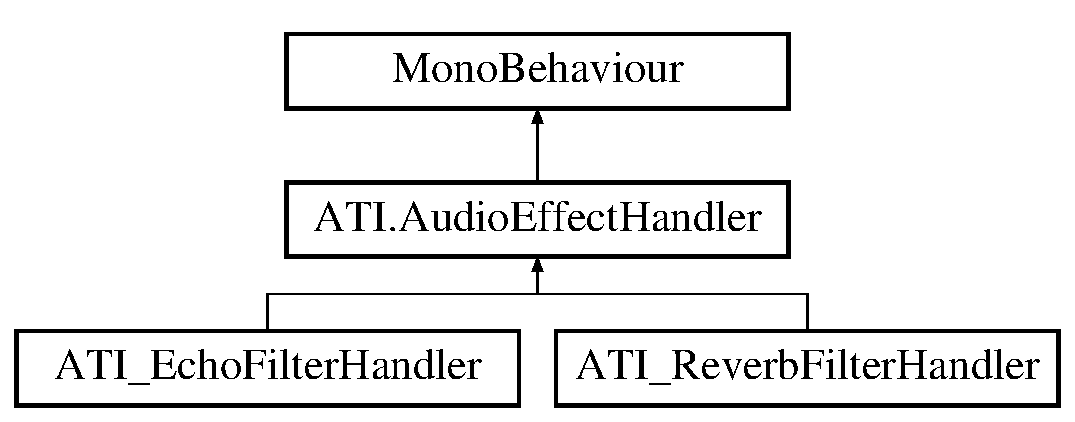
\includegraphics[height=3.000000cm]{class_a_t_i_1_1_audio_effect_handler}
\end{center}
\end{figure}
\subsection*{Public Member Functions}
\begin{DoxyCompactItemize}
\item 
void \hyperlink{class_a_t_i_1_1_audio_effect_handler_ad47b6cefdd2bab8bec233069269e76e4}{Start} ()
\item 
void \hyperlink{class_a_t_i_1_1_audio_effect_handler_aa698c6c69066c8e3f2caa9beeea51569}{On\+Toggle} (bool a\+Enabled)
\item 
void \hyperlink{class_a_t_i_1_1_audio_effect_handler_a298f455be06ae16a870fa291337a77c6}{Handle\+Audio\+Effect\+Parameter\+Change} (\hyperlink{class_a_t_i_a1123d61b8dceb5867a3683e8d2224ee1}{Audio\+Effect\+Parameter\+Type} a\+Type, float a\+Value)
\end{DoxyCompactItemize}
\subsection*{Protected Member Functions}
\begin{DoxyCompactItemize}
\item 
virtual void \hyperlink{class_a_t_i_1_1_audio_effect_handler_ae8a88211ac0910dc4b7752667abb2f84}{Handle\+Decay\+Change} (float a\+Value)
\item 
virtual void \hyperlink{class_a_t_i_1_1_audio_effect_handler_a5371fca4c2e86cecfc264dfc7559b6bd}{Handle\+Delay\+Change} (float a\+Value)
\item 
virtual void \hyperlink{class_a_t_i_1_1_audio_effect_handler_a8d83371e2e982373b4eb04198a8514fb}{Handle\+Dry\+Mix\+Change} (float a\+Value)
\item 
virtual void \hyperlink{class_a_t_i_1_1_audio_effect_handler_a630d6f0e674c531ad0c138181609a895}{Handle\+Wet\+Mix\+Change} (float a\+Value)
\item 
virtual void \hyperlink{class_a_t_i_1_1_audio_effect_handler_abf6b4a6ead7e60bbaea15f94936c316e}{Handle\+Dry\+Level\+Change} (float a\+Value)
\item 
virtual void \hyperlink{class_a_t_i_1_1_audio_effect_handler_a416ae6f8266224b0d6cd71cba1020001}{Handle\+Room\+Change} (float a\+Value)
\item 
virtual void \hyperlink{class_a_t_i_1_1_audio_effect_handler_af3f3b123b89b6e53dce5a7c22190f5b6}{Handle\+Room\+H\+F\+Change} (float a\+Value)
\item 
virtual void \hyperlink{class_a_t_i_1_1_audio_effect_handler_a35173ee088bc2459907af3521bcd69ac}{Handle\+Decay\+Time\+Change} (float a\+Value)
\item 
virtual void \hyperlink{class_a_t_i_1_1_audio_effect_handler_af00cbc35b44d68de0d2d0497e1defa3a}{Handle\+Decay\+H\+F\+Ratio\+Change} (float a\+Value)
\item 
virtual void \hyperlink{class_a_t_i_1_1_audio_effect_handler_af50ba52dba236a3b711172fd6bbc1bab}{Handle\+Reflections\+Change} (float a\+Value)
\item 
virtual void \hyperlink{class_a_t_i_1_1_audio_effect_handler_ada336ed04fdb3360de3026ba8659c409}{Handle\+Reflect\+Delay\+Change} (float a\+Value)
\item 
virtual void \hyperlink{class_a_t_i_1_1_audio_effect_handler_aee7aa84aa7d433a7f7264aff131d5a6a}{Handle\+Reverb\+Change} (float a\+Value)
\item 
virtual void \hyperlink{class_a_t_i_1_1_audio_effect_handler_a03f47bb2ac36fc9c672ccddd76af6e6a}{Handle\+Reverb\+Delay\+Change} (float a\+Value)
\item 
virtual void \hyperlink{class_a_t_i_1_1_audio_effect_handler_adcf777de620420b6c411350db0eca2aa}{Handle\+Diffusion\+Change} (float a\+Value)
\item 
virtual void \hyperlink{class_a_t_i_1_1_audio_effect_handler_acdbfbd384e2fdb5bd43ad977e264500a}{Handle\+Density\+Change} (float a\+Value)
\item 
virtual void \hyperlink{class_a_t_i_1_1_audio_effect_handler_a183b75c93279e0d6322a0e005c590891}{Handle\+H\+F\+Reference\+Change} (float a\+Value)
\item 
virtual void \hyperlink{class_a_t_i_1_1_audio_effect_handler_ae2648d4ab8a617cbc509f7cfc38f21f6}{Handle\+Room\+L\+F\+Change} (float a\+Value)
\item 
virtual void \hyperlink{class_a_t_i_1_1_audio_effect_handler_a8414b47429880ba18133571c86cf14ab}{Handle\+L\+F\+Reference\+Change} (float a\+Value)
\item 
virtual void \hyperlink{class_a_t_i_1_1_audio_effect_handler_a9f2b5ce4ce7b2e3a7cca147a87733a77}{Set\+Default\+Parameters} ()
\item 
virtual void \hyperlink{class_a_t_i_1_1_audio_effect_handler_aa038c62089df16a01d2749986649db11}{Handle\+Scene\+Load} ()
\item 
virtual void \hyperlink{class_a_t_i_1_1_audio_effect_handler_aab43cfccb835b9630456eb4590626e6d}{Send\+Parameters\+To\+V\+IM} ()
\item 
virtual void \hyperlink{class_a_t_i_1_1_audio_effect_handler_abccfc2e809d0d6b643704f7391461cd7}{Turn\+On\+Effect} ()
\item 
virtual void \hyperlink{class_a_t_i_1_1_audio_effect_handler_aed35f816dce2a75b857c79ffbb6cc677}{Turn\+Off\+Effect} ()
\end{DoxyCompactItemize}
\subsection*{Protected Attributes}
\begin{DoxyCompactItemize}
\item 
Async\+Operation \hyperlink{class_a_t_i_1_1_audio_effect_handler_a64e2617a1b7c1e6f4631a6aee98fbf3e}{m\+Scene\+Load\+Operation} = null
\item 
\hyperlink{class_a_t_i_1_1_audio_effect_parameter_trigger}{Audio\+Effect\+Parameter\+Trigger} \mbox{[}$\,$\mbox{]} \hyperlink{class_a_t_i_1_1_audio_effect_handler_a1db04dc85daf07d045117d9bc585e944}{m\+Triggers} = null
\item 
bool \hyperlink{class_a_t_i_1_1_audio_effect_handler_a378c463b827ad6e41d09a4ec2caff351}{m\+Enabled} = false
\item 
Game\+Object \hyperlink{class_a_t_i_1_1_audio_effect_handler_a02ca13686cb3fc7bf152051ec881b0ed}{m\+Param\+Object} = null
\item 
Image \hyperlink{class_a_t_i_1_1_audio_effect_handler_aa5bf03976a14594f089aac5681c15a83}{m\+Toggle\+Image} = null
\item 
Sprite \mbox{[}$\,$\mbox{]} \hyperlink{class_a_t_i_1_1_audio_effect_handler_a6e1cfd5449b82870eacd7404a158c7a7}{m\+Button\+Images} = null
\item 
string \hyperlink{class_a_t_i_1_1_audio_effect_handler_a674c38f29ef923e6c9487c2dc991a8b6}{m\+Param\+Scene\+Name} = null
\item 
Toggle \hyperlink{class_a_t_i_1_1_audio_effect_handler_ae5f6b965d3401ff17fde2e77f33f9109}{m\+Toggle\+Switch} = null
\item 
\hyperlink{class_virtual_instrument_manager}{Virtual\+Instrument\+Manager} \hyperlink{class_a_t_i_1_1_audio_effect_handler_a6b5b6149cc376ff0f750ade08ba23bce}{m\+V\+IM} = null
\end{DoxyCompactItemize}
\subsection*{Private Member Functions}
\begin{DoxyCompactItemize}
\item 
void \hyperlink{class_a_t_i_1_1_audio_effect_handler_af41e912b86543e7c074531d2cd3f88dc}{Update} ()
\end{DoxyCompactItemize}


\subsection{Detailed Description}


Definition at line 376 of file A\+T\+I.\+cs.



\subsection{Member Function Documentation}
\mbox{\Hypertarget{class_a_t_i_1_1_audio_effect_handler_a298f455be06ae16a870fa291337a77c6}\label{class_a_t_i_1_1_audio_effect_handler_a298f455be06ae16a870fa291337a77c6}} 
\index{A\+T\+I\+::\+Audio\+Effect\+Handler@{A\+T\+I\+::\+Audio\+Effect\+Handler}!Handle\+Audio\+Effect\+Parameter\+Change@{Handle\+Audio\+Effect\+Parameter\+Change}}
\index{Handle\+Audio\+Effect\+Parameter\+Change@{Handle\+Audio\+Effect\+Parameter\+Change}!A\+T\+I\+::\+Audio\+Effect\+Handler@{A\+T\+I\+::\+Audio\+Effect\+Handler}}
\subsubsection{\texorpdfstring{Handle\+Audio\+Effect\+Parameter\+Change()}{HandleAudioEffectParameterChange()}}
{\footnotesize\ttfamily void A\+T\+I.\+Audio\+Effect\+Handler.\+Handle\+Audio\+Effect\+Parameter\+Change (\begin{DoxyParamCaption}\item[{\hyperlink{class_a_t_i_a1123d61b8dceb5867a3683e8d2224ee1}{Audio\+Effect\+Parameter\+Type}}]{a\+Type,  }\item[{float}]{a\+Value }\end{DoxyParamCaption})}



Definition at line 488 of file A\+T\+I.\+cs.



Referenced by A\+T\+I.\+Audio\+Effect\+Parameter\+Trigger.\+Send\+Input\+Field\+Change\+To\+Handler(), and A\+T\+I.\+Audio\+Effect\+Parameter\+Trigger.\+Send\+Slider\+Change\+To\+Handler().


\begin{DoxyCode}
489         \{
490             \textcolor{keywordflow}{switch}( aType )
491             \{
492                 \textcolor{keywordflow}{case} \hyperlink{class_a_t_i_a1123d61b8dceb5867a3683e8d2224ee1}{AudioEffectParameterType}.Decay:
493                     \hyperlink{class_a_t_i_1_1_audio_effect_handler_ae8a88211ac0910dc4b7752667abb2f84}{HandleDecayChange}( aValue );
494                     \textcolor{keywordflow}{break};
495                 \textcolor{keywordflow}{case} \hyperlink{class_a_t_i_a1123d61b8dceb5867a3683e8d2224ee1}{AudioEffectParameterType}.Delay:
496                     \hyperlink{class_a_t_i_1_1_audio_effect_handler_a5371fca4c2e86cecfc264dfc7559b6bd}{HandleDelayChange}( aValue );
497                     \textcolor{keywordflow}{break};
498                 \textcolor{keywordflow}{case} \hyperlink{class_a_t_i_a1123d61b8dceb5867a3683e8d2224ee1}{AudioEffectParameterType}.DryMix:
499                     \hyperlink{class_a_t_i_1_1_audio_effect_handler_a8d83371e2e982373b4eb04198a8514fb}{HandleDryMixChange}( aValue );
500                     \textcolor{keywordflow}{break};
501                 \textcolor{keywordflow}{case} \hyperlink{class_a_t_i_a1123d61b8dceb5867a3683e8d2224ee1}{AudioEffectParameterType}.WetMix:
502                     \hyperlink{class_a_t_i_1_1_audio_effect_handler_a630d6f0e674c531ad0c138181609a895}{HandleWetMixChange}( aValue );
503                     \textcolor{keywordflow}{break};
504                 \textcolor{keywordflow}{case} \hyperlink{class_a_t_i_a1123d61b8dceb5867a3683e8d2224ee1}{AudioEffectParameterType}.DryLevel:
505                     \hyperlink{class_a_t_i_1_1_audio_effect_handler_abf6b4a6ead7e60bbaea15f94936c316e}{HandleDryLevelChange}( aValue );
506                     \textcolor{keywordflow}{break};
507                 \textcolor{keywordflow}{case} \hyperlink{class_a_t_i_a1123d61b8dceb5867a3683e8d2224ee1}{AudioEffectParameterType}.Room:
508                     \hyperlink{class_a_t_i_1_1_audio_effect_handler_a416ae6f8266224b0d6cd71cba1020001}{HandleRoomChange}( aValue );
509                     \textcolor{keywordflow}{break};
510                 \textcolor{keywordflow}{case} \hyperlink{class_a_t_i_a1123d61b8dceb5867a3683e8d2224ee1}{AudioEffectParameterType}.RoomHF:
511                     \hyperlink{class_a_t_i_1_1_audio_effect_handler_af3f3b123b89b6e53dce5a7c22190f5b6}{HandleRoomHFChange}( aValue );
512                     \textcolor{keywordflow}{break};
513                 \textcolor{keywordflow}{case} \hyperlink{class_a_t_i_a1123d61b8dceb5867a3683e8d2224ee1}{AudioEffectParameterType}.DecayTime:
514                     \hyperlink{class_a_t_i_1_1_audio_effect_handler_a35173ee088bc2459907af3521bcd69ac}{HandleDecayTimeChange}( aValue );
515                     \textcolor{keywordflow}{break};
516                 \textcolor{keywordflow}{case} \hyperlink{class_a_t_i_a1123d61b8dceb5867a3683e8d2224ee1}{AudioEffectParameterType}.DecayHFRatio:
517                     \hyperlink{class_a_t_i_1_1_audio_effect_handler_af00cbc35b44d68de0d2d0497e1defa3a}{HandleDecayHFRatioChange}( aValue );
518                     \textcolor{keywordflow}{break};
519                 \textcolor{keywordflow}{case} \hyperlink{class_a_t_i_a1123d61b8dceb5867a3683e8d2224ee1}{AudioEffectParameterType}.Reflections:
520                     \hyperlink{class_a_t_i_1_1_audio_effect_handler_af50ba52dba236a3b711172fd6bbc1bab}{HandleReflectionsChange}( aValue );
521                     \textcolor{keywordflow}{break};
522                 \textcolor{keywordflow}{case} \hyperlink{class_a_t_i_a1123d61b8dceb5867a3683e8d2224ee1}{AudioEffectParameterType}.ReflectDelay:
523                     \hyperlink{class_a_t_i_1_1_audio_effect_handler_ada336ed04fdb3360de3026ba8659c409}{HandleReflectDelayChange}( aValue );
524                     \textcolor{keywordflow}{break};
525                 \textcolor{keywordflow}{case} \hyperlink{class_a_t_i_a1123d61b8dceb5867a3683e8d2224ee1}{AudioEffectParameterType}.Reverb:
526                     \hyperlink{class_a_t_i_1_1_audio_effect_handler_aee7aa84aa7d433a7f7264aff131d5a6a}{HandleReverbChange}( aValue );
527                     \textcolor{keywordflow}{break};
528                 \textcolor{keywordflow}{case} \hyperlink{class_a_t_i_a1123d61b8dceb5867a3683e8d2224ee1}{AudioEffectParameterType}.ReverbDelay:
529                     \hyperlink{class_a_t_i_1_1_audio_effect_handler_a03f47bb2ac36fc9c672ccddd76af6e6a}{HandleReverbDelayChange}( aValue );
530                     \textcolor{keywordflow}{break};
531                 \textcolor{keywordflow}{case} \hyperlink{class_a_t_i_a1123d61b8dceb5867a3683e8d2224ee1}{AudioEffectParameterType}.Diffusion:
532                     \hyperlink{class_a_t_i_1_1_audio_effect_handler_adcf777de620420b6c411350db0eca2aa}{HandleDiffusionChange}( aValue );
533                     \textcolor{keywordflow}{break};
534                 \textcolor{keywordflow}{case} \hyperlink{class_a_t_i_a1123d61b8dceb5867a3683e8d2224ee1}{AudioEffectParameterType}.Density:
535                     \hyperlink{class_a_t_i_1_1_audio_effect_handler_acdbfbd384e2fdb5bd43ad977e264500a}{HandleDensityChange}( aValue );
536                     \textcolor{keywordflow}{break};
537                 \textcolor{keywordflow}{case} \hyperlink{class_a_t_i_a1123d61b8dceb5867a3683e8d2224ee1}{AudioEffectParameterType}.HFReference:
538                     \hyperlink{class_a_t_i_1_1_audio_effect_handler_a183b75c93279e0d6322a0e005c590891}{HandleHFReferenceChange}( aValue );
539                     \textcolor{keywordflow}{break};
540                 \textcolor{keywordflow}{case} \hyperlink{class_a_t_i_a1123d61b8dceb5867a3683e8d2224ee1}{AudioEffectParameterType}.RoomLF:
541                     \hyperlink{class_a_t_i_1_1_audio_effect_handler_ae2648d4ab8a617cbc509f7cfc38f21f6}{HandleRoomLFChange}( aValue );
542                     \textcolor{keywordflow}{break};
543                 \textcolor{keywordflow}{case} \hyperlink{class_a_t_i_a1123d61b8dceb5867a3683e8d2224ee1}{AudioEffectParameterType}.LFReference:
544                     \hyperlink{class_a_t_i_1_1_audio_effect_handler_a8414b47429880ba18133571c86cf14ab}{HandleLFReferenceChange}( aValue );
545                     \textcolor{keywordflow}{break};
546                 \textcolor{keywordflow}{default}:
547                     \textcolor{keywordflow}{break};
548             \}
549         \}
\end{DoxyCode}
\mbox{\Hypertarget{class_a_t_i_1_1_audio_effect_handler_ae8a88211ac0910dc4b7752667abb2f84}\label{class_a_t_i_1_1_audio_effect_handler_ae8a88211ac0910dc4b7752667abb2f84}} 
\index{A\+T\+I\+::\+Audio\+Effect\+Handler@{A\+T\+I\+::\+Audio\+Effect\+Handler}!Handle\+Decay\+Change@{Handle\+Decay\+Change}}
\index{Handle\+Decay\+Change@{Handle\+Decay\+Change}!A\+T\+I\+::\+Audio\+Effect\+Handler@{A\+T\+I\+::\+Audio\+Effect\+Handler}}
\subsubsection{\texorpdfstring{Handle\+Decay\+Change()}{HandleDecayChange()}}
{\footnotesize\ttfamily virtual void A\+T\+I.\+Audio\+Effect\+Handler.\+Handle\+Decay\+Change (\begin{DoxyParamCaption}\item[{float}]{a\+Value }\end{DoxyParamCaption})\hspace{0.3cm}{\ttfamily [protected]}, {\ttfamily [virtual]}}



Reimplemented in \hyperlink{class_a_t_i___echo_filter_handler_a280746246e42f85d36f96640a7148705}{A\+T\+I\+\_\+\+Echo\+Filter\+Handler}.



Definition at line 554 of file A\+T\+I.\+cs.


\begin{DoxyCode}
554 \{ \}
\end{DoxyCode}
\mbox{\Hypertarget{class_a_t_i_1_1_audio_effect_handler_af00cbc35b44d68de0d2d0497e1defa3a}\label{class_a_t_i_1_1_audio_effect_handler_af00cbc35b44d68de0d2d0497e1defa3a}} 
\index{A\+T\+I\+::\+Audio\+Effect\+Handler@{A\+T\+I\+::\+Audio\+Effect\+Handler}!Handle\+Decay\+H\+F\+Ratio\+Change@{Handle\+Decay\+H\+F\+Ratio\+Change}}
\index{Handle\+Decay\+H\+F\+Ratio\+Change@{Handle\+Decay\+H\+F\+Ratio\+Change}!A\+T\+I\+::\+Audio\+Effect\+Handler@{A\+T\+I\+::\+Audio\+Effect\+Handler}}
\subsubsection{\texorpdfstring{Handle\+Decay\+H\+F\+Ratio\+Change()}{HandleDecayHFRatioChange()}}
{\footnotesize\ttfamily virtual void A\+T\+I.\+Audio\+Effect\+Handler.\+Handle\+Decay\+H\+F\+Ratio\+Change (\begin{DoxyParamCaption}\item[{float}]{a\+Value }\end{DoxyParamCaption})\hspace{0.3cm}{\ttfamily [protected]}, {\ttfamily [virtual]}}



Reimplemented in \hyperlink{class_a_t_i___reverb_filter_handler_a68dab792c963c33be3618c9595a6a734}{A\+T\+I\+\_\+\+Reverb\+Filter\+Handler}.



Definition at line 562 of file A\+T\+I.\+cs.


\begin{DoxyCode}
562 \{ \}
\end{DoxyCode}
\mbox{\Hypertarget{class_a_t_i_1_1_audio_effect_handler_a35173ee088bc2459907af3521bcd69ac}\label{class_a_t_i_1_1_audio_effect_handler_a35173ee088bc2459907af3521bcd69ac}} 
\index{A\+T\+I\+::\+Audio\+Effect\+Handler@{A\+T\+I\+::\+Audio\+Effect\+Handler}!Handle\+Decay\+Time\+Change@{Handle\+Decay\+Time\+Change}}
\index{Handle\+Decay\+Time\+Change@{Handle\+Decay\+Time\+Change}!A\+T\+I\+::\+Audio\+Effect\+Handler@{A\+T\+I\+::\+Audio\+Effect\+Handler}}
\subsubsection{\texorpdfstring{Handle\+Decay\+Time\+Change()}{HandleDecayTimeChange()}}
{\footnotesize\ttfamily virtual void A\+T\+I.\+Audio\+Effect\+Handler.\+Handle\+Decay\+Time\+Change (\begin{DoxyParamCaption}\item[{float}]{a\+Value }\end{DoxyParamCaption})\hspace{0.3cm}{\ttfamily [protected]}, {\ttfamily [virtual]}}



Reimplemented in \hyperlink{class_a_t_i___reverb_filter_handler_a30a45fb9d8bbd7e10054eaa4595666b3}{A\+T\+I\+\_\+\+Reverb\+Filter\+Handler}.



Definition at line 561 of file A\+T\+I.\+cs.


\begin{DoxyCode}
561 \{ \}
\end{DoxyCode}
\mbox{\Hypertarget{class_a_t_i_1_1_audio_effect_handler_a5371fca4c2e86cecfc264dfc7559b6bd}\label{class_a_t_i_1_1_audio_effect_handler_a5371fca4c2e86cecfc264dfc7559b6bd}} 
\index{A\+T\+I\+::\+Audio\+Effect\+Handler@{A\+T\+I\+::\+Audio\+Effect\+Handler}!Handle\+Delay\+Change@{Handle\+Delay\+Change}}
\index{Handle\+Delay\+Change@{Handle\+Delay\+Change}!A\+T\+I\+::\+Audio\+Effect\+Handler@{A\+T\+I\+::\+Audio\+Effect\+Handler}}
\subsubsection{\texorpdfstring{Handle\+Delay\+Change()}{HandleDelayChange()}}
{\footnotesize\ttfamily virtual void A\+T\+I.\+Audio\+Effect\+Handler.\+Handle\+Delay\+Change (\begin{DoxyParamCaption}\item[{float}]{a\+Value }\end{DoxyParamCaption})\hspace{0.3cm}{\ttfamily [protected]}, {\ttfamily [virtual]}}



Reimplemented in \hyperlink{class_a_t_i___echo_filter_handler_a33447b03218ff2945e5f8cea0f8f0d45}{A\+T\+I\+\_\+\+Echo\+Filter\+Handler}.



Definition at line 555 of file A\+T\+I.\+cs.


\begin{DoxyCode}
555 \{ \}
\end{DoxyCode}
\mbox{\Hypertarget{class_a_t_i_1_1_audio_effect_handler_acdbfbd384e2fdb5bd43ad977e264500a}\label{class_a_t_i_1_1_audio_effect_handler_acdbfbd384e2fdb5bd43ad977e264500a}} 
\index{A\+T\+I\+::\+Audio\+Effect\+Handler@{A\+T\+I\+::\+Audio\+Effect\+Handler}!Handle\+Density\+Change@{Handle\+Density\+Change}}
\index{Handle\+Density\+Change@{Handle\+Density\+Change}!A\+T\+I\+::\+Audio\+Effect\+Handler@{A\+T\+I\+::\+Audio\+Effect\+Handler}}
\subsubsection{\texorpdfstring{Handle\+Density\+Change()}{HandleDensityChange()}}
{\footnotesize\ttfamily virtual void A\+T\+I.\+Audio\+Effect\+Handler.\+Handle\+Density\+Change (\begin{DoxyParamCaption}\item[{float}]{a\+Value }\end{DoxyParamCaption})\hspace{0.3cm}{\ttfamily [protected]}, {\ttfamily [virtual]}}



Reimplemented in \hyperlink{class_a_t_i___reverb_filter_handler_a4a95ee1076720663fbe84e624385e636}{A\+T\+I\+\_\+\+Reverb\+Filter\+Handler}.



Definition at line 568 of file A\+T\+I.\+cs.


\begin{DoxyCode}
568 \{ \}
\end{DoxyCode}
\mbox{\Hypertarget{class_a_t_i_1_1_audio_effect_handler_adcf777de620420b6c411350db0eca2aa}\label{class_a_t_i_1_1_audio_effect_handler_adcf777de620420b6c411350db0eca2aa}} 
\index{A\+T\+I\+::\+Audio\+Effect\+Handler@{A\+T\+I\+::\+Audio\+Effect\+Handler}!Handle\+Diffusion\+Change@{Handle\+Diffusion\+Change}}
\index{Handle\+Diffusion\+Change@{Handle\+Diffusion\+Change}!A\+T\+I\+::\+Audio\+Effect\+Handler@{A\+T\+I\+::\+Audio\+Effect\+Handler}}
\subsubsection{\texorpdfstring{Handle\+Diffusion\+Change()}{HandleDiffusionChange()}}
{\footnotesize\ttfamily virtual void A\+T\+I.\+Audio\+Effect\+Handler.\+Handle\+Diffusion\+Change (\begin{DoxyParamCaption}\item[{float}]{a\+Value }\end{DoxyParamCaption})\hspace{0.3cm}{\ttfamily [protected]}, {\ttfamily [virtual]}}



Reimplemented in \hyperlink{class_a_t_i___reverb_filter_handler_a6cd79af5d1835bd4ab8a6420fed82e53}{A\+T\+I\+\_\+\+Reverb\+Filter\+Handler}.



Definition at line 567 of file A\+T\+I.\+cs.


\begin{DoxyCode}
567 \{ \}
\end{DoxyCode}
\mbox{\Hypertarget{class_a_t_i_1_1_audio_effect_handler_abf6b4a6ead7e60bbaea15f94936c316e}\label{class_a_t_i_1_1_audio_effect_handler_abf6b4a6ead7e60bbaea15f94936c316e}} 
\index{A\+T\+I\+::\+Audio\+Effect\+Handler@{A\+T\+I\+::\+Audio\+Effect\+Handler}!Handle\+Dry\+Level\+Change@{Handle\+Dry\+Level\+Change}}
\index{Handle\+Dry\+Level\+Change@{Handle\+Dry\+Level\+Change}!A\+T\+I\+::\+Audio\+Effect\+Handler@{A\+T\+I\+::\+Audio\+Effect\+Handler}}
\subsubsection{\texorpdfstring{Handle\+Dry\+Level\+Change()}{HandleDryLevelChange()}}
{\footnotesize\ttfamily virtual void A\+T\+I.\+Audio\+Effect\+Handler.\+Handle\+Dry\+Level\+Change (\begin{DoxyParamCaption}\item[{float}]{a\+Value }\end{DoxyParamCaption})\hspace{0.3cm}{\ttfamily [protected]}, {\ttfamily [virtual]}}



Reimplemented in \hyperlink{class_a_t_i___reverb_filter_handler_a0af6a4381b725183fdb7cc8589a9f71f}{A\+T\+I\+\_\+\+Reverb\+Filter\+Handler}.



Definition at line 558 of file A\+T\+I.\+cs.


\begin{DoxyCode}
558 \{ \}
\end{DoxyCode}
\mbox{\Hypertarget{class_a_t_i_1_1_audio_effect_handler_a8d83371e2e982373b4eb04198a8514fb}\label{class_a_t_i_1_1_audio_effect_handler_a8d83371e2e982373b4eb04198a8514fb}} 
\index{A\+T\+I\+::\+Audio\+Effect\+Handler@{A\+T\+I\+::\+Audio\+Effect\+Handler}!Handle\+Dry\+Mix\+Change@{Handle\+Dry\+Mix\+Change}}
\index{Handle\+Dry\+Mix\+Change@{Handle\+Dry\+Mix\+Change}!A\+T\+I\+::\+Audio\+Effect\+Handler@{A\+T\+I\+::\+Audio\+Effect\+Handler}}
\subsubsection{\texorpdfstring{Handle\+Dry\+Mix\+Change()}{HandleDryMixChange()}}
{\footnotesize\ttfamily virtual void A\+T\+I.\+Audio\+Effect\+Handler.\+Handle\+Dry\+Mix\+Change (\begin{DoxyParamCaption}\item[{float}]{a\+Value }\end{DoxyParamCaption})\hspace{0.3cm}{\ttfamily [protected]}, {\ttfamily [virtual]}}



Reimplemented in \hyperlink{class_a_t_i___echo_filter_handler_afc69af9ea7789eb655c01c851594716a}{A\+T\+I\+\_\+\+Echo\+Filter\+Handler}.



Definition at line 556 of file A\+T\+I.\+cs.


\begin{DoxyCode}
556 \{ \}
\end{DoxyCode}
\mbox{\Hypertarget{class_a_t_i_1_1_audio_effect_handler_a183b75c93279e0d6322a0e005c590891}\label{class_a_t_i_1_1_audio_effect_handler_a183b75c93279e0d6322a0e005c590891}} 
\index{A\+T\+I\+::\+Audio\+Effect\+Handler@{A\+T\+I\+::\+Audio\+Effect\+Handler}!Handle\+H\+F\+Reference\+Change@{Handle\+H\+F\+Reference\+Change}}
\index{Handle\+H\+F\+Reference\+Change@{Handle\+H\+F\+Reference\+Change}!A\+T\+I\+::\+Audio\+Effect\+Handler@{A\+T\+I\+::\+Audio\+Effect\+Handler}}
\subsubsection{\texorpdfstring{Handle\+H\+F\+Reference\+Change()}{HandleHFReferenceChange()}}
{\footnotesize\ttfamily virtual void A\+T\+I.\+Audio\+Effect\+Handler.\+Handle\+H\+F\+Reference\+Change (\begin{DoxyParamCaption}\item[{float}]{a\+Value }\end{DoxyParamCaption})\hspace{0.3cm}{\ttfamily [protected]}, {\ttfamily [virtual]}}



Reimplemented in \hyperlink{class_a_t_i___reverb_filter_handler_a4cb8ab454ef637beb189053a0877c8c6}{A\+T\+I\+\_\+\+Reverb\+Filter\+Handler}.



Definition at line 569 of file A\+T\+I.\+cs.


\begin{DoxyCode}
569 \{ \}
\end{DoxyCode}
\mbox{\Hypertarget{class_a_t_i_1_1_audio_effect_handler_a8414b47429880ba18133571c86cf14ab}\label{class_a_t_i_1_1_audio_effect_handler_a8414b47429880ba18133571c86cf14ab}} 
\index{A\+T\+I\+::\+Audio\+Effect\+Handler@{A\+T\+I\+::\+Audio\+Effect\+Handler}!Handle\+L\+F\+Reference\+Change@{Handle\+L\+F\+Reference\+Change}}
\index{Handle\+L\+F\+Reference\+Change@{Handle\+L\+F\+Reference\+Change}!A\+T\+I\+::\+Audio\+Effect\+Handler@{A\+T\+I\+::\+Audio\+Effect\+Handler}}
\subsubsection{\texorpdfstring{Handle\+L\+F\+Reference\+Change()}{HandleLFReferenceChange()}}
{\footnotesize\ttfamily virtual void A\+T\+I.\+Audio\+Effect\+Handler.\+Handle\+L\+F\+Reference\+Change (\begin{DoxyParamCaption}\item[{float}]{a\+Value }\end{DoxyParamCaption})\hspace{0.3cm}{\ttfamily [protected]}, {\ttfamily [virtual]}}



Reimplemented in \hyperlink{class_a_t_i___reverb_filter_handler_abf697e814be89c3bd354deaccb237746}{A\+T\+I\+\_\+\+Reverb\+Filter\+Handler}.



Definition at line 571 of file A\+T\+I.\+cs.


\begin{DoxyCode}
571 \{ \}
\end{DoxyCode}
\mbox{\Hypertarget{class_a_t_i_1_1_audio_effect_handler_ada336ed04fdb3360de3026ba8659c409}\label{class_a_t_i_1_1_audio_effect_handler_ada336ed04fdb3360de3026ba8659c409}} 
\index{A\+T\+I\+::\+Audio\+Effect\+Handler@{A\+T\+I\+::\+Audio\+Effect\+Handler}!Handle\+Reflect\+Delay\+Change@{Handle\+Reflect\+Delay\+Change}}
\index{Handle\+Reflect\+Delay\+Change@{Handle\+Reflect\+Delay\+Change}!A\+T\+I\+::\+Audio\+Effect\+Handler@{A\+T\+I\+::\+Audio\+Effect\+Handler}}
\subsubsection{\texorpdfstring{Handle\+Reflect\+Delay\+Change()}{HandleReflectDelayChange()}}
{\footnotesize\ttfamily virtual void A\+T\+I.\+Audio\+Effect\+Handler.\+Handle\+Reflect\+Delay\+Change (\begin{DoxyParamCaption}\item[{float}]{a\+Value }\end{DoxyParamCaption})\hspace{0.3cm}{\ttfamily [protected]}, {\ttfamily [virtual]}}



Reimplemented in \hyperlink{class_a_t_i___reverb_filter_handler_a83de9c38851424d66456dfe98163dfde}{A\+T\+I\+\_\+\+Reverb\+Filter\+Handler}.



Definition at line 564 of file A\+T\+I.\+cs.


\begin{DoxyCode}
564 \{ \}
\end{DoxyCode}
\mbox{\Hypertarget{class_a_t_i_1_1_audio_effect_handler_af50ba52dba236a3b711172fd6bbc1bab}\label{class_a_t_i_1_1_audio_effect_handler_af50ba52dba236a3b711172fd6bbc1bab}} 
\index{A\+T\+I\+::\+Audio\+Effect\+Handler@{A\+T\+I\+::\+Audio\+Effect\+Handler}!Handle\+Reflections\+Change@{Handle\+Reflections\+Change}}
\index{Handle\+Reflections\+Change@{Handle\+Reflections\+Change}!A\+T\+I\+::\+Audio\+Effect\+Handler@{A\+T\+I\+::\+Audio\+Effect\+Handler}}
\subsubsection{\texorpdfstring{Handle\+Reflections\+Change()}{HandleReflectionsChange()}}
{\footnotesize\ttfamily virtual void A\+T\+I.\+Audio\+Effect\+Handler.\+Handle\+Reflections\+Change (\begin{DoxyParamCaption}\item[{float}]{a\+Value }\end{DoxyParamCaption})\hspace{0.3cm}{\ttfamily [protected]}, {\ttfamily [virtual]}}



Reimplemented in \hyperlink{class_a_t_i___reverb_filter_handler_a8db38f7eafd2b1ed0a5f8d488244d83a}{A\+T\+I\+\_\+\+Reverb\+Filter\+Handler}.



Definition at line 563 of file A\+T\+I.\+cs.


\begin{DoxyCode}
563 \{ \}
\end{DoxyCode}
\mbox{\Hypertarget{class_a_t_i_1_1_audio_effect_handler_aee7aa84aa7d433a7f7264aff131d5a6a}\label{class_a_t_i_1_1_audio_effect_handler_aee7aa84aa7d433a7f7264aff131d5a6a}} 
\index{A\+T\+I\+::\+Audio\+Effect\+Handler@{A\+T\+I\+::\+Audio\+Effect\+Handler}!Handle\+Reverb\+Change@{Handle\+Reverb\+Change}}
\index{Handle\+Reverb\+Change@{Handle\+Reverb\+Change}!A\+T\+I\+::\+Audio\+Effect\+Handler@{A\+T\+I\+::\+Audio\+Effect\+Handler}}
\subsubsection{\texorpdfstring{Handle\+Reverb\+Change()}{HandleReverbChange()}}
{\footnotesize\ttfamily virtual void A\+T\+I.\+Audio\+Effect\+Handler.\+Handle\+Reverb\+Change (\begin{DoxyParamCaption}\item[{float}]{a\+Value }\end{DoxyParamCaption})\hspace{0.3cm}{\ttfamily [protected]}, {\ttfamily [virtual]}}



Reimplemented in \hyperlink{class_a_t_i___reverb_filter_handler_ae228f1d67c8efd950a3b2c594d5dd9f8}{A\+T\+I\+\_\+\+Reverb\+Filter\+Handler}.



Definition at line 565 of file A\+T\+I.\+cs.


\begin{DoxyCode}
565 \{ \}
\end{DoxyCode}
\mbox{\Hypertarget{class_a_t_i_1_1_audio_effect_handler_a03f47bb2ac36fc9c672ccddd76af6e6a}\label{class_a_t_i_1_1_audio_effect_handler_a03f47bb2ac36fc9c672ccddd76af6e6a}} 
\index{A\+T\+I\+::\+Audio\+Effect\+Handler@{A\+T\+I\+::\+Audio\+Effect\+Handler}!Handle\+Reverb\+Delay\+Change@{Handle\+Reverb\+Delay\+Change}}
\index{Handle\+Reverb\+Delay\+Change@{Handle\+Reverb\+Delay\+Change}!A\+T\+I\+::\+Audio\+Effect\+Handler@{A\+T\+I\+::\+Audio\+Effect\+Handler}}
\subsubsection{\texorpdfstring{Handle\+Reverb\+Delay\+Change()}{HandleReverbDelayChange()}}
{\footnotesize\ttfamily virtual void A\+T\+I.\+Audio\+Effect\+Handler.\+Handle\+Reverb\+Delay\+Change (\begin{DoxyParamCaption}\item[{float}]{a\+Value }\end{DoxyParamCaption})\hspace{0.3cm}{\ttfamily [protected]}, {\ttfamily [virtual]}}



Reimplemented in \hyperlink{class_a_t_i___reverb_filter_handler_af126757d50b12330f868d2178bdb5d6c}{A\+T\+I\+\_\+\+Reverb\+Filter\+Handler}.



Definition at line 566 of file A\+T\+I.\+cs.


\begin{DoxyCode}
566 \{ \}
\end{DoxyCode}
\mbox{\Hypertarget{class_a_t_i_1_1_audio_effect_handler_a416ae6f8266224b0d6cd71cba1020001}\label{class_a_t_i_1_1_audio_effect_handler_a416ae6f8266224b0d6cd71cba1020001}} 
\index{A\+T\+I\+::\+Audio\+Effect\+Handler@{A\+T\+I\+::\+Audio\+Effect\+Handler}!Handle\+Room\+Change@{Handle\+Room\+Change}}
\index{Handle\+Room\+Change@{Handle\+Room\+Change}!A\+T\+I\+::\+Audio\+Effect\+Handler@{A\+T\+I\+::\+Audio\+Effect\+Handler}}
\subsubsection{\texorpdfstring{Handle\+Room\+Change()}{HandleRoomChange()}}
{\footnotesize\ttfamily virtual void A\+T\+I.\+Audio\+Effect\+Handler.\+Handle\+Room\+Change (\begin{DoxyParamCaption}\item[{float}]{a\+Value }\end{DoxyParamCaption})\hspace{0.3cm}{\ttfamily [protected]}, {\ttfamily [virtual]}}



Reimplemented in \hyperlink{class_a_t_i___reverb_filter_handler_a2100456086ad1adf704bf88d71dbe490}{A\+T\+I\+\_\+\+Reverb\+Filter\+Handler}.



Definition at line 559 of file A\+T\+I.\+cs.


\begin{DoxyCode}
559 \{ \}
\end{DoxyCode}
\mbox{\Hypertarget{class_a_t_i_1_1_audio_effect_handler_af3f3b123b89b6e53dce5a7c22190f5b6}\label{class_a_t_i_1_1_audio_effect_handler_af3f3b123b89b6e53dce5a7c22190f5b6}} 
\index{A\+T\+I\+::\+Audio\+Effect\+Handler@{A\+T\+I\+::\+Audio\+Effect\+Handler}!Handle\+Room\+H\+F\+Change@{Handle\+Room\+H\+F\+Change}}
\index{Handle\+Room\+H\+F\+Change@{Handle\+Room\+H\+F\+Change}!A\+T\+I\+::\+Audio\+Effect\+Handler@{A\+T\+I\+::\+Audio\+Effect\+Handler}}
\subsubsection{\texorpdfstring{Handle\+Room\+H\+F\+Change()}{HandleRoomHFChange()}}
{\footnotesize\ttfamily virtual void A\+T\+I.\+Audio\+Effect\+Handler.\+Handle\+Room\+H\+F\+Change (\begin{DoxyParamCaption}\item[{float}]{a\+Value }\end{DoxyParamCaption})\hspace{0.3cm}{\ttfamily [protected]}, {\ttfamily [virtual]}}



Reimplemented in \hyperlink{class_a_t_i___reverb_filter_handler_a587ab9596231ed2ff9e3628bbc59d510}{A\+T\+I\+\_\+\+Reverb\+Filter\+Handler}.



Definition at line 560 of file A\+T\+I.\+cs.


\begin{DoxyCode}
560 \{ \}
\end{DoxyCode}
\mbox{\Hypertarget{class_a_t_i_1_1_audio_effect_handler_ae2648d4ab8a617cbc509f7cfc38f21f6}\label{class_a_t_i_1_1_audio_effect_handler_ae2648d4ab8a617cbc509f7cfc38f21f6}} 
\index{A\+T\+I\+::\+Audio\+Effect\+Handler@{A\+T\+I\+::\+Audio\+Effect\+Handler}!Handle\+Room\+L\+F\+Change@{Handle\+Room\+L\+F\+Change}}
\index{Handle\+Room\+L\+F\+Change@{Handle\+Room\+L\+F\+Change}!A\+T\+I\+::\+Audio\+Effect\+Handler@{A\+T\+I\+::\+Audio\+Effect\+Handler}}
\subsubsection{\texorpdfstring{Handle\+Room\+L\+F\+Change()}{HandleRoomLFChange()}}
{\footnotesize\ttfamily virtual void A\+T\+I.\+Audio\+Effect\+Handler.\+Handle\+Room\+L\+F\+Change (\begin{DoxyParamCaption}\item[{float}]{a\+Value }\end{DoxyParamCaption})\hspace{0.3cm}{\ttfamily [protected]}, {\ttfamily [virtual]}}



Reimplemented in \hyperlink{class_a_t_i___reverb_filter_handler_a52fe6f9775f8e51296580f7a96b47bdb}{A\+T\+I\+\_\+\+Reverb\+Filter\+Handler}.



Definition at line 570 of file A\+T\+I.\+cs.


\begin{DoxyCode}
570 \{ \}
\end{DoxyCode}
\mbox{\Hypertarget{class_a_t_i_1_1_audio_effect_handler_aa038c62089df16a01d2749986649db11}\label{class_a_t_i_1_1_audio_effect_handler_aa038c62089df16a01d2749986649db11}} 
\index{A\+T\+I\+::\+Audio\+Effect\+Handler@{A\+T\+I\+::\+Audio\+Effect\+Handler}!Handle\+Scene\+Load@{Handle\+Scene\+Load}}
\index{Handle\+Scene\+Load@{Handle\+Scene\+Load}!A\+T\+I\+::\+Audio\+Effect\+Handler@{A\+T\+I\+::\+Audio\+Effect\+Handler}}
\subsubsection{\texorpdfstring{Handle\+Scene\+Load()}{HandleSceneLoad()}}
{\footnotesize\ttfamily virtual void A\+T\+I.\+Audio\+Effect\+Handler.\+Handle\+Scene\+Load (\begin{DoxyParamCaption}{ }\end{DoxyParamCaption})\hspace{0.3cm}{\ttfamily [protected]}, {\ttfamily [virtual]}}



Reimplemented in \hyperlink{class_a_t_i___reverb_filter_handler_a084dca3566139f350b0372d3ee85af84}{A\+T\+I\+\_\+\+Reverb\+Filter\+Handler}, and \hyperlink{class_a_t_i___echo_filter_handler_aef6df1fd85fb153d232191f1bd4de5f3}{A\+T\+I\+\_\+\+Echo\+Filter\+Handler}.



Definition at line 573 of file A\+T\+I.\+cs.


\begin{DoxyCode}
573 \{ \}
\end{DoxyCode}
\mbox{\Hypertarget{class_a_t_i_1_1_audio_effect_handler_a630d6f0e674c531ad0c138181609a895}\label{class_a_t_i_1_1_audio_effect_handler_a630d6f0e674c531ad0c138181609a895}} 
\index{A\+T\+I\+::\+Audio\+Effect\+Handler@{A\+T\+I\+::\+Audio\+Effect\+Handler}!Handle\+Wet\+Mix\+Change@{Handle\+Wet\+Mix\+Change}}
\index{Handle\+Wet\+Mix\+Change@{Handle\+Wet\+Mix\+Change}!A\+T\+I\+::\+Audio\+Effect\+Handler@{A\+T\+I\+::\+Audio\+Effect\+Handler}}
\subsubsection{\texorpdfstring{Handle\+Wet\+Mix\+Change()}{HandleWetMixChange()}}
{\footnotesize\ttfamily virtual void A\+T\+I.\+Audio\+Effect\+Handler.\+Handle\+Wet\+Mix\+Change (\begin{DoxyParamCaption}\item[{float}]{a\+Value }\end{DoxyParamCaption})\hspace{0.3cm}{\ttfamily [protected]}, {\ttfamily [virtual]}}



Reimplemented in \hyperlink{class_a_t_i___echo_filter_handler_ab64eed11cb12db663a9485bc4bc26fb9}{A\+T\+I\+\_\+\+Echo\+Filter\+Handler}.



Definition at line 557 of file A\+T\+I.\+cs.


\begin{DoxyCode}
557 \{ \}
\end{DoxyCode}
\mbox{\Hypertarget{class_a_t_i_1_1_audio_effect_handler_aa698c6c69066c8e3f2caa9beeea51569}\label{class_a_t_i_1_1_audio_effect_handler_aa698c6c69066c8e3f2caa9beeea51569}} 
\index{A\+T\+I\+::\+Audio\+Effect\+Handler@{A\+T\+I\+::\+Audio\+Effect\+Handler}!On\+Toggle@{On\+Toggle}}
\index{On\+Toggle@{On\+Toggle}!A\+T\+I\+::\+Audio\+Effect\+Handler@{A\+T\+I\+::\+Audio\+Effect\+Handler}}
\subsubsection{\texorpdfstring{On\+Toggle()}{OnToggle()}}
{\footnotesize\ttfamily void A\+T\+I.\+Audio\+Effect\+Handler.\+On\+Toggle (\begin{DoxyParamCaption}\item[{bool}]{a\+Enabled }\end{DoxyParamCaption})}



Definition at line 455 of file A\+T\+I.\+cs.


\begin{DoxyCode}
456         \{
457             \textcolor{comment}{// If the effect is now on, handle turning on the effect.}
458             \textcolor{keywordflow}{if}( aEnabled )
459             \{
460                 \textcolor{comment}{// Sanity Check.}
461                 \textcolor{keywordflow}{if}( \hyperlink{class_a_t_i_1_1_audio_effect_handler_a674c38f29ef923e6c9487c2dc991a8b6}{mParamSceneName} == null )
462                 \{
463                     Assert.IsTrue( \textcolor{keyword}{false}, \textcolor{stringliteral}{"Turned on an uninitialized audio effect!"} );
464                     \textcolor{keywordflow}{return};
465                 \}
466 
467                 \textcolor{comment}{// Make the subclass turn on the effect.}
468                 \hyperlink{class_a_t_i_1_1_audio_effect_handler_abccfc2e809d0d6b643704f7391461cd7}{TurnOnEffect}();
469 
470                 \textcolor{comment}{// Start loading the parameter scene.}
471                 \hyperlink{class_a_t_i_1_1_audio_effect_handler_a64e2617a1b7c1e6f4631a6aee98fbf3e}{mSceneLoadOperation} = SceneManager.LoadSceneAsync( 
      \hyperlink{class_a_t_i_1_1_audio_effect_handler_a674c38f29ef923e6c9487c2dc991a8b6}{mParamSceneName}, LoadSceneMode.Additive );
472             \}
473             \textcolor{comment}{// If the effect is now off, then turn off the effect.}
474             \textcolor{keywordflow}{else}
475             \{
476                 \textcolor{comment}{// Unload the parameter scene.}
477                 \hyperlink{class_a_t_i_1_1_audio_effect_handler_a02ca13686cb3fc7bf152051ec881b0ed}{mParamObject}.transform.SetParent( SceneManager.GetSceneByName( 
      \hyperlink{class_a_t_i_1_1_audio_effect_handler_a674c38f29ef923e6c9487c2dc991a8b6}{mParamSceneName} ).GetRootGameObjects()[0].transform );
478                 SceneManager.UnloadSceneAsync( \hyperlink{class_a_t_i_1_1_audio_effect_handler_a674c38f29ef923e6c9487c2dc991a8b6}{mParamSceneName} );
479 
480                 \textcolor{comment}{// Make the subclass turn off the effect.}
481                 \hyperlink{class_a_t_i_1_1_audio_effect_handler_aed35f816dce2a75b857c79ffbb6cc677}{TurnOffEffect}();
482             \}
483         \}
\end{DoxyCode}
\mbox{\Hypertarget{class_a_t_i_1_1_audio_effect_handler_aab43cfccb835b9630456eb4590626e6d}\label{class_a_t_i_1_1_audio_effect_handler_aab43cfccb835b9630456eb4590626e6d}} 
\index{A\+T\+I\+::\+Audio\+Effect\+Handler@{A\+T\+I\+::\+Audio\+Effect\+Handler}!Send\+Parameters\+To\+V\+IM@{Send\+Parameters\+To\+V\+IM}}
\index{Send\+Parameters\+To\+V\+IM@{Send\+Parameters\+To\+V\+IM}!A\+T\+I\+::\+Audio\+Effect\+Handler@{A\+T\+I\+::\+Audio\+Effect\+Handler}}
\subsubsection{\texorpdfstring{Send\+Parameters\+To\+V\+I\+M()}{SendParametersToVIM()}}
{\footnotesize\ttfamily virtual void A\+T\+I.\+Audio\+Effect\+Handler.\+Send\+Parameters\+To\+V\+IM (\begin{DoxyParamCaption}{ }\end{DoxyParamCaption})\hspace{0.3cm}{\ttfamily [protected]}, {\ttfamily [virtual]}}



Reimplemented in \hyperlink{class_a_t_i___reverb_filter_handler_aacb469dc3038fca616d638f6a5a04a30}{A\+T\+I\+\_\+\+Reverb\+Filter\+Handler}, and \hyperlink{class_a_t_i___echo_filter_handler_afacef95c6ac470707d2bd092031efac0}{A\+T\+I\+\_\+\+Echo\+Filter\+Handler}.



Definition at line 574 of file A\+T\+I.\+cs.


\begin{DoxyCode}
574 \{ \}
\end{DoxyCode}
\mbox{\Hypertarget{class_a_t_i_1_1_audio_effect_handler_a9f2b5ce4ce7b2e3a7cca147a87733a77}\label{class_a_t_i_1_1_audio_effect_handler_a9f2b5ce4ce7b2e3a7cca147a87733a77}} 
\index{A\+T\+I\+::\+Audio\+Effect\+Handler@{A\+T\+I\+::\+Audio\+Effect\+Handler}!Set\+Default\+Parameters@{Set\+Default\+Parameters}}
\index{Set\+Default\+Parameters@{Set\+Default\+Parameters}!A\+T\+I\+::\+Audio\+Effect\+Handler@{A\+T\+I\+::\+Audio\+Effect\+Handler}}
\subsubsection{\texorpdfstring{Set\+Default\+Parameters()}{SetDefaultParameters()}}
{\footnotesize\ttfamily virtual void A\+T\+I.\+Audio\+Effect\+Handler.\+Set\+Default\+Parameters (\begin{DoxyParamCaption}{ }\end{DoxyParamCaption})\hspace{0.3cm}{\ttfamily [protected]}, {\ttfamily [virtual]}}



Reimplemented in \hyperlink{class_a_t_i___reverb_filter_handler_a69a75dcda06ae1597030e0ceaf84e1ae}{A\+T\+I\+\_\+\+Reverb\+Filter\+Handler}, and \hyperlink{class_a_t_i___echo_filter_handler_a55aed0339fe1f3cdbea2b810a2d74cd4}{A\+T\+I\+\_\+\+Echo\+Filter\+Handler}.



Definition at line 572 of file A\+T\+I.\+cs.


\begin{DoxyCode}
572 \{ \}
\end{DoxyCode}
\mbox{\Hypertarget{class_a_t_i_1_1_audio_effect_handler_ad47b6cefdd2bab8bec233069269e76e4}\label{class_a_t_i_1_1_audio_effect_handler_ad47b6cefdd2bab8bec233069269e76e4}} 
\index{A\+T\+I\+::\+Audio\+Effect\+Handler@{A\+T\+I\+::\+Audio\+Effect\+Handler}!Start@{Start}}
\index{Start@{Start}!A\+T\+I\+::\+Audio\+Effect\+Handler@{A\+T\+I\+::\+Audio\+Effect\+Handler}}
\subsubsection{\texorpdfstring{Start()}{Start()}}
{\footnotesize\ttfamily void A\+T\+I.\+Audio\+Effect\+Handler.\+Start (\begin{DoxyParamCaption}{ }\end{DoxyParamCaption})}



Definition at line 396 of file A\+T\+I.\+cs.


\begin{DoxyCode}
397         \{
398             \textcolor{comment}{// Get the virtual instrument manager.}
399             \hyperlink{class_a_t_i_1_1_audio_effect_handler_a6b5b6149cc376ff0f750ade08ba23bce}{mVIM} = GameObject.Find( \textcolor{stringliteral}{"VirtualInstrumentManager"} ).GetComponent<
      \hyperlink{class_virtual_instrument_manager}{VirtualInstrumentManager}>();
400 
401             \textcolor{comment}{// Get the toggle switch and add its listener.}
402             \hyperlink{class_a_t_i_1_1_audio_effect_handler_ae5f6b965d3401ff17fde2e77f33f9109}{mToggleSwitch} = gameObject.transform.GetChild( 0 ).GetComponent<Toggle>();
403             mToggleSwitch.onValueChanged.AddListener( \hyperlink{class_a_t_i_1_1_audio_effect_handler_aa698c6c69066c8e3f2caa9beeea51569}{OnToggle} );
404 
405             \textcolor{comment}{// Get the toggle image.}
406             \hyperlink{class_a_t_i_1_1_audio_effect_handler_aa5bf03976a14594f089aac5681c15a83}{mToggleImage} = mToggleSwitch.transform.GetChild( 0 ).GetComponent<Image>();
407 
408             \textcolor{comment}{// Load the images for the toggle switch.}
409             \hyperlink{class_a_t_i_1_1_audio_effect_handler_a6e1cfd5449b82870eacd7404a158c7a7}{mButtonImages} = \textcolor{keyword}{new} Sprite[2];
410             mButtonImages[0] = Resources.Load<Sprite>( \textcolor{stringliteral}{"Audio/Images/off\_button"} );
411             mButtonImages[1] = Resources.Load<Sprite>( \textcolor{stringliteral}{"Audio/Images/on\_button"} );
412 
413             \textcolor{comment}{// Set the default parameters.}
414             \hyperlink{class_a_t_i_1_1_audio_effect_handler_a9f2b5ce4ce7b2e3a7cca147a87733a77}{SetDefaultParameters}();
415 
416         \}
\end{DoxyCode}
\mbox{\Hypertarget{class_a_t_i_1_1_audio_effect_handler_aed35f816dce2a75b857c79ffbb6cc677}\label{class_a_t_i_1_1_audio_effect_handler_aed35f816dce2a75b857c79ffbb6cc677}} 
\index{A\+T\+I\+::\+Audio\+Effect\+Handler@{A\+T\+I\+::\+Audio\+Effect\+Handler}!Turn\+Off\+Effect@{Turn\+Off\+Effect}}
\index{Turn\+Off\+Effect@{Turn\+Off\+Effect}!A\+T\+I\+::\+Audio\+Effect\+Handler@{A\+T\+I\+::\+Audio\+Effect\+Handler}}
\subsubsection{\texorpdfstring{Turn\+Off\+Effect()}{TurnOffEffect()}}
{\footnotesize\ttfamily virtual void A\+T\+I.\+Audio\+Effect\+Handler.\+Turn\+Off\+Effect (\begin{DoxyParamCaption}{ }\end{DoxyParamCaption})\hspace{0.3cm}{\ttfamily [protected]}, {\ttfamily [virtual]}}



Reimplemented in \hyperlink{class_a_t_i___reverb_filter_handler_a87b5c207c0ec0422ce8bea66a38334e2}{A\+T\+I\+\_\+\+Reverb\+Filter\+Handler}, and \hyperlink{class_a_t_i___echo_filter_handler_aefc1d2ab19273b9606c09eff2db13165}{A\+T\+I\+\_\+\+Echo\+Filter\+Handler}.



Definition at line 576 of file A\+T\+I.\+cs.


\begin{DoxyCode}
576 \{ \}
\end{DoxyCode}
\mbox{\Hypertarget{class_a_t_i_1_1_audio_effect_handler_abccfc2e809d0d6b643704f7391461cd7}\label{class_a_t_i_1_1_audio_effect_handler_abccfc2e809d0d6b643704f7391461cd7}} 
\index{A\+T\+I\+::\+Audio\+Effect\+Handler@{A\+T\+I\+::\+Audio\+Effect\+Handler}!Turn\+On\+Effect@{Turn\+On\+Effect}}
\index{Turn\+On\+Effect@{Turn\+On\+Effect}!A\+T\+I\+::\+Audio\+Effect\+Handler@{A\+T\+I\+::\+Audio\+Effect\+Handler}}
\subsubsection{\texorpdfstring{Turn\+On\+Effect()}{TurnOnEffect()}}
{\footnotesize\ttfamily virtual void A\+T\+I.\+Audio\+Effect\+Handler.\+Turn\+On\+Effect (\begin{DoxyParamCaption}{ }\end{DoxyParamCaption})\hspace{0.3cm}{\ttfamily [protected]}, {\ttfamily [virtual]}}



Reimplemented in \hyperlink{class_a_t_i___reverb_filter_handler_aa25fcaa9c07d614b869334e1db14f7d6}{A\+T\+I\+\_\+\+Reverb\+Filter\+Handler}, and \hyperlink{class_a_t_i___echo_filter_handler_af759b786ad6e701f816264fefdddb078}{A\+T\+I\+\_\+\+Echo\+Filter\+Handler}.



Definition at line 575 of file A\+T\+I.\+cs.


\begin{DoxyCode}
575 \{ \}
\end{DoxyCode}
\mbox{\Hypertarget{class_a_t_i_1_1_audio_effect_handler_af41e912b86543e7c074531d2cd3f88dc}\label{class_a_t_i_1_1_audio_effect_handler_af41e912b86543e7c074531d2cd3f88dc}} 
\index{A\+T\+I\+::\+Audio\+Effect\+Handler@{A\+T\+I\+::\+Audio\+Effect\+Handler}!Update@{Update}}
\index{Update@{Update}!A\+T\+I\+::\+Audio\+Effect\+Handler@{A\+T\+I\+::\+Audio\+Effect\+Handler}}
\subsubsection{\texorpdfstring{Update()}{Update()}}
{\footnotesize\ttfamily void A\+T\+I.\+Audio\+Effect\+Handler.\+Update (\begin{DoxyParamCaption}{ }\end{DoxyParamCaption})\hspace{0.3cm}{\ttfamily [private]}}



Definition at line 419 of file A\+T\+I.\+cs.


\begin{DoxyCode}
420         \{
421             \textcolor{comment}{// If we are currently loading a scene, then see if it is done.}
422             \textcolor{keywordflow}{if}( \hyperlink{class_a_t_i_1_1_audio_effect_handler_a64e2617a1b7c1e6f4631a6aee98fbf3e}{mSceneLoadOperation} != null && \hyperlink{class_a_t_i_1_1_audio_effect_handler_a378c463b827ad6e41d09a4ec2caff351}{mEnabled} )
423             \{
424                 \textcolor{comment}{// If the scene is done, then get the parameter container and set it }
425                 \textcolor{comment}{// underneath this object.}
426                 \textcolor{keywordflow}{if}( \hyperlink{class_a_t_i_1_1_audio_effect_handler_a64e2617a1b7c1e6f4631a6aee98fbf3e}{mSceneLoadOperation}.isDone )
427                 \{
428                     \textcolor{comment}{// Get the parameter container.}
429                     \hyperlink{class_a_t_i_1_1_audio_effect_handler_a02ca13686cb3fc7bf152051ec881b0ed}{mParamObject} = SceneManager.GetSceneByName( 
      \hyperlink{class_a_t_i_1_1_audio_effect_handler_a674c38f29ef923e6c9487c2dc991a8b6}{mParamSceneName} ).GetRootGameObjects()[0].transform.GetChild( 0 ).gameObject;
430                     \hyperlink{class_a_t_i_1_1_audio_effect_handler_a02ca13686cb3fc7bf152051ec881b0ed}{mParamObject}.transform.SetParent( gameObject.transform, \textcolor{keyword}{true} );
431 
432                     \textcolor{comment}{// Set the container's position.}
433                     Vector3 temp = \textcolor{keyword}{new} Vector3( 0f, 0f, 0f );
434                     temp.y -= ( ( \hyperlink{class_a_t_i_1_1_audio_effect_handler_a02ca13686cb3fc7bf152051ec881b0ed}{mParamObject}.GetComponent<RectTransform>().rect.height * 
      \hyperlink{class_a_t_i_1_1_audio_effect_handler_a02ca13686cb3fc7bf152051ec881b0ed}{mParamObject}.transform.localScale.y / 2f ) +
435                         ( gameObject.GetComponent<RectTransform>().rect.height / 2f ) );
436                     temp.x += ( ( \hyperlink{class_a_t_i_1_1_audio_effect_handler_a02ca13686cb3fc7bf152051ec881b0ed}{mParamObject}.GetComponent<RectTransform>().rect.width / 2f ) 
      -
437                         ( gameObject.GetComponent<RectTransform>().rect.width / 2f ) );
438                     \hyperlink{class_a_t_i_1_1_audio_effect_handler_a02ca13686cb3fc7bf152051ec881b0ed}{mParamObject}.transform.localPosition = temp;
439 
440                     \textcolor{comment}{// Reset the scene load operation.}
441                     \hyperlink{class_a_t_i_1_1_audio_effect_handler_a64e2617a1b7c1e6f4631a6aee98fbf3e}{mSceneLoadOperation} = null;
442 
443                     \textcolor{comment}{// Make the specific subclass handle the scene being loaded.}
444                     \hyperlink{class_a_t_i_1_1_audio_effect_handler_aa038c62089df16a01d2749986649db11}{HandleSceneLoad}();
445                 \}
446             \}
447         \}
\end{DoxyCode}


\subsection{Member Data Documentation}
\mbox{\Hypertarget{class_a_t_i_1_1_audio_effect_handler_a6e1cfd5449b82870eacd7404a158c7a7}\label{class_a_t_i_1_1_audio_effect_handler_a6e1cfd5449b82870eacd7404a158c7a7}} 
\index{A\+T\+I\+::\+Audio\+Effect\+Handler@{A\+T\+I\+::\+Audio\+Effect\+Handler}!m\+Button\+Images@{m\+Button\+Images}}
\index{m\+Button\+Images@{m\+Button\+Images}!A\+T\+I\+::\+Audio\+Effect\+Handler@{A\+T\+I\+::\+Audio\+Effect\+Handler}}
\subsubsection{\texorpdfstring{m\+Button\+Images}{mButtonImages}}
{\footnotesize\ttfamily Sprite \mbox{[}$\,$\mbox{]} A\+T\+I.\+Audio\+Effect\+Handler.\+m\+Button\+Images = null\hspace{0.3cm}{\ttfamily [protected]}}



Definition at line 386 of file A\+T\+I.\+cs.



Referenced by A\+T\+I\+\_\+\+Echo\+Filter\+Handler.\+Turn\+Off\+Effect(), A\+T\+I\+\_\+\+Reverb\+Filter\+Handler.\+Turn\+Off\+Effect(), A\+T\+I\+\_\+\+Echo\+Filter\+Handler.\+Turn\+On\+Effect(), and A\+T\+I\+\_\+\+Reverb\+Filter\+Handler.\+Turn\+On\+Effect().

\mbox{\Hypertarget{class_a_t_i_1_1_audio_effect_handler_a378c463b827ad6e41d09a4ec2caff351}\label{class_a_t_i_1_1_audio_effect_handler_a378c463b827ad6e41d09a4ec2caff351}} 
\index{A\+T\+I\+::\+Audio\+Effect\+Handler@{A\+T\+I\+::\+Audio\+Effect\+Handler}!m\+Enabled@{m\+Enabled}}
\index{m\+Enabled@{m\+Enabled}!A\+T\+I\+::\+Audio\+Effect\+Handler@{A\+T\+I\+::\+Audio\+Effect\+Handler}}
\subsubsection{\texorpdfstring{m\+Enabled}{mEnabled}}
{\footnotesize\ttfamily bool A\+T\+I.\+Audio\+Effect\+Handler.\+m\+Enabled = false\hspace{0.3cm}{\ttfamily [protected]}}



Definition at line 383 of file A\+T\+I.\+cs.



Referenced by A\+T\+I\+\_\+\+Echo\+Filter\+Handler.\+Turn\+Off\+Effect(), A\+T\+I\+\_\+\+Reverb\+Filter\+Handler.\+Turn\+Off\+Effect(), A\+T\+I\+\_\+\+Echo\+Filter\+Handler.\+Turn\+On\+Effect(), and A\+T\+I\+\_\+\+Reverb\+Filter\+Handler.\+Turn\+On\+Effect().

\mbox{\Hypertarget{class_a_t_i_1_1_audio_effect_handler_a02ca13686cb3fc7bf152051ec881b0ed}\label{class_a_t_i_1_1_audio_effect_handler_a02ca13686cb3fc7bf152051ec881b0ed}} 
\index{A\+T\+I\+::\+Audio\+Effect\+Handler@{A\+T\+I\+::\+Audio\+Effect\+Handler}!m\+Param\+Object@{m\+Param\+Object}}
\index{m\+Param\+Object@{m\+Param\+Object}!A\+T\+I\+::\+Audio\+Effect\+Handler@{A\+T\+I\+::\+Audio\+Effect\+Handler}}
\subsubsection{\texorpdfstring{m\+Param\+Object}{mParamObject}}
{\footnotesize\ttfamily Game\+Object A\+T\+I.\+Audio\+Effect\+Handler.\+m\+Param\+Object = null\hspace{0.3cm}{\ttfamily [protected]}}



Definition at line 384 of file A\+T\+I.\+cs.



Referenced by A\+T\+I\+\_\+\+Echo\+Filter\+Handler.\+Handle\+Scene\+Load(), A\+T\+I\+\_\+\+Reverb\+Filter\+Handler.\+Handle\+Scene\+Load(), A\+T\+I\+\_\+\+Echo\+Filter\+Handler.\+Turn\+Off\+Effect(), and A\+T\+I\+\_\+\+Reverb\+Filter\+Handler.\+Turn\+Off\+Effect().

\mbox{\Hypertarget{class_a_t_i_1_1_audio_effect_handler_a674c38f29ef923e6c9487c2dc991a8b6}\label{class_a_t_i_1_1_audio_effect_handler_a674c38f29ef923e6c9487c2dc991a8b6}} 
\index{A\+T\+I\+::\+Audio\+Effect\+Handler@{A\+T\+I\+::\+Audio\+Effect\+Handler}!m\+Param\+Scene\+Name@{m\+Param\+Scene\+Name}}
\index{m\+Param\+Scene\+Name@{m\+Param\+Scene\+Name}!A\+T\+I\+::\+Audio\+Effect\+Handler@{A\+T\+I\+::\+Audio\+Effect\+Handler}}
\subsubsection{\texorpdfstring{m\+Param\+Scene\+Name}{mParamSceneName}}
{\footnotesize\ttfamily string A\+T\+I.\+Audio\+Effect\+Handler.\+m\+Param\+Scene\+Name = null\hspace{0.3cm}{\ttfamily [protected]}}



Definition at line 387 of file A\+T\+I.\+cs.



Referenced by A\+T\+I\+\_\+\+Echo\+Filter\+Handler.\+Start(), and A\+T\+I\+\_\+\+Reverb\+Filter\+Handler.\+Start().

\mbox{\Hypertarget{class_a_t_i_1_1_audio_effect_handler_a64e2617a1b7c1e6f4631a6aee98fbf3e}\label{class_a_t_i_1_1_audio_effect_handler_a64e2617a1b7c1e6f4631a6aee98fbf3e}} 
\index{A\+T\+I\+::\+Audio\+Effect\+Handler@{A\+T\+I\+::\+Audio\+Effect\+Handler}!m\+Scene\+Load\+Operation@{m\+Scene\+Load\+Operation}}
\index{m\+Scene\+Load\+Operation@{m\+Scene\+Load\+Operation}!A\+T\+I\+::\+Audio\+Effect\+Handler@{A\+T\+I\+::\+Audio\+Effect\+Handler}}
\subsubsection{\texorpdfstring{m\+Scene\+Load\+Operation}{mSceneLoadOperation}}
{\footnotesize\ttfamily Async\+Operation A\+T\+I.\+Audio\+Effect\+Handler.\+m\+Scene\+Load\+Operation = null\hspace{0.3cm}{\ttfamily [protected]}}



Definition at line 381 of file A\+T\+I.\+cs.

\mbox{\Hypertarget{class_a_t_i_1_1_audio_effect_handler_aa5bf03976a14594f089aac5681c15a83}\label{class_a_t_i_1_1_audio_effect_handler_aa5bf03976a14594f089aac5681c15a83}} 
\index{A\+T\+I\+::\+Audio\+Effect\+Handler@{A\+T\+I\+::\+Audio\+Effect\+Handler}!m\+Toggle\+Image@{m\+Toggle\+Image}}
\index{m\+Toggle\+Image@{m\+Toggle\+Image}!A\+T\+I\+::\+Audio\+Effect\+Handler@{A\+T\+I\+::\+Audio\+Effect\+Handler}}
\subsubsection{\texorpdfstring{m\+Toggle\+Image}{mToggleImage}}
{\footnotesize\ttfamily Image A\+T\+I.\+Audio\+Effect\+Handler.\+m\+Toggle\+Image = null\hspace{0.3cm}{\ttfamily [protected]}}



Definition at line 385 of file A\+T\+I.\+cs.



Referenced by A\+T\+I\+\_\+\+Echo\+Filter\+Handler.\+Turn\+Off\+Effect(), A\+T\+I\+\_\+\+Reverb\+Filter\+Handler.\+Turn\+Off\+Effect(), A\+T\+I\+\_\+\+Echo\+Filter\+Handler.\+Turn\+On\+Effect(), and A\+T\+I\+\_\+\+Reverb\+Filter\+Handler.\+Turn\+On\+Effect().

\mbox{\Hypertarget{class_a_t_i_1_1_audio_effect_handler_ae5f6b965d3401ff17fde2e77f33f9109}\label{class_a_t_i_1_1_audio_effect_handler_ae5f6b965d3401ff17fde2e77f33f9109}} 
\index{A\+T\+I\+::\+Audio\+Effect\+Handler@{A\+T\+I\+::\+Audio\+Effect\+Handler}!m\+Toggle\+Switch@{m\+Toggle\+Switch}}
\index{m\+Toggle\+Switch@{m\+Toggle\+Switch}!A\+T\+I\+::\+Audio\+Effect\+Handler@{A\+T\+I\+::\+Audio\+Effect\+Handler}}
\subsubsection{\texorpdfstring{m\+Toggle\+Switch}{mToggleSwitch}}
{\footnotesize\ttfamily Toggle A\+T\+I.\+Audio\+Effect\+Handler.\+m\+Toggle\+Switch = null\hspace{0.3cm}{\ttfamily [protected]}}



Definition at line 388 of file A\+T\+I.\+cs.

\mbox{\Hypertarget{class_a_t_i_1_1_audio_effect_handler_a1db04dc85daf07d045117d9bc585e944}\label{class_a_t_i_1_1_audio_effect_handler_a1db04dc85daf07d045117d9bc585e944}} 
\index{A\+T\+I\+::\+Audio\+Effect\+Handler@{A\+T\+I\+::\+Audio\+Effect\+Handler}!m\+Triggers@{m\+Triggers}}
\index{m\+Triggers@{m\+Triggers}!A\+T\+I\+::\+Audio\+Effect\+Handler@{A\+T\+I\+::\+Audio\+Effect\+Handler}}
\subsubsection{\texorpdfstring{m\+Triggers}{mTriggers}}
{\footnotesize\ttfamily \hyperlink{class_a_t_i_1_1_audio_effect_parameter_trigger}{Audio\+Effect\+Parameter\+Trigger} \mbox{[}$\,$\mbox{]} A\+T\+I.\+Audio\+Effect\+Handler.\+m\+Triggers = null\hspace{0.3cm}{\ttfamily [protected]}}



Definition at line 382 of file A\+T\+I.\+cs.



Referenced by A\+T\+I\+\_\+\+Echo\+Filter\+Handler.\+Handle\+Scene\+Load(), A\+T\+I\+\_\+\+Reverb\+Filter\+Handler.\+Handle\+Scene\+Load(), A\+T\+I\+\_\+\+Echo\+Filter\+Handler.\+Turn\+Off\+Effect(), and A\+T\+I\+\_\+\+Reverb\+Filter\+Handler.\+Turn\+Off\+Effect().

\mbox{\Hypertarget{class_a_t_i_1_1_audio_effect_handler_a6b5b6149cc376ff0f750ade08ba23bce}\label{class_a_t_i_1_1_audio_effect_handler_a6b5b6149cc376ff0f750ade08ba23bce}} 
\index{A\+T\+I\+::\+Audio\+Effect\+Handler@{A\+T\+I\+::\+Audio\+Effect\+Handler}!m\+V\+IM@{m\+V\+IM}}
\index{m\+V\+IM@{m\+V\+IM}!A\+T\+I\+::\+Audio\+Effect\+Handler@{A\+T\+I\+::\+Audio\+Effect\+Handler}}
\subsubsection{\texorpdfstring{m\+V\+IM}{mVIM}}
{\footnotesize\ttfamily \hyperlink{class_virtual_instrument_manager}{Virtual\+Instrument\+Manager} A\+T\+I.\+Audio\+Effect\+Handler.\+m\+V\+IM = null\hspace{0.3cm}{\ttfamily [protected]}}



Definition at line 389 of file A\+T\+I.\+cs.



Referenced by A\+T\+I\+\_\+\+Echo\+Filter\+Handler.\+Send\+Parameters\+To\+V\+I\+M(), and A\+T\+I\+\_\+\+Reverb\+Filter\+Handler.\+Send\+Parameters\+To\+V\+I\+M().



The documentation for this class was generated from the following file\+:\begin{DoxyCompactItemize}
\item 
D\+:/\+Documents/\+School Documents/2017\+Spring/\+E\+E\+C\+S542/\+V\+R\+Piano\+Project/\+Assets/\+Scripts/\+Audio/\+Testing/\hyperlink{_a_t_i_8cs}{A\+T\+I.\+cs}\end{DoxyCompactItemize}

\hypertarget{class_a_t_i_1_1_audio_effect_parameter_trigger}{}\section{A\+T\+I.\+Audio\+Effect\+Parameter\+Trigger Class Reference}
\label{class_a_t_i_1_1_audio_effect_parameter_trigger}\index{A\+T\+I.\+Audio\+Effect\+Parameter\+Trigger@{A\+T\+I.\+Audio\+Effect\+Parameter\+Trigger}}
Inheritance diagram for A\+T\+I.\+Audio\+Effect\+Parameter\+Trigger\+:\begin{figure}[H]
\begin{center}
\leavevmode
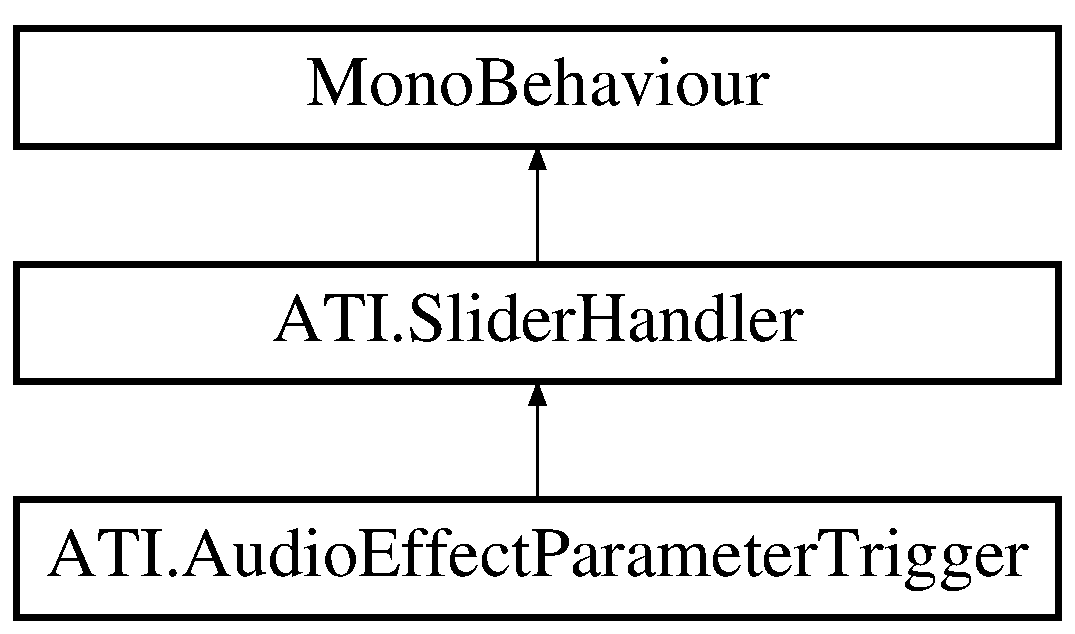
\includegraphics[height=3.000000cm]{class_a_t_i_1_1_audio_effect_parameter_trigger}
\end{center}
\end{figure}
\subsection*{Public Member Functions}
\begin{DoxyCompactItemize}
\item 
void \hyperlink{class_a_t_i_1_1_audio_effect_parameter_trigger_a69dc7845ba6454981ce5454ca55b4cb1}{Set\+Handler} (\hyperlink{class_a_t_i_1_1_audio_effect_handler}{Audio\+Effect\+Handler} a\+Handler)
\item 
void \hyperlink{class_a_t_i_1_1_audio_effect_parameter_trigger_a3b61498abf2b3e3c8cba23e296ff9273}{Set\+Range} (float a\+Lowest, float a\+Highest)
\item 
void \hyperlink{class_a_t_i_1_1_audio_effect_parameter_trigger_a12b9e1d13260a5970f5effed71b9a216}{Set\+Type} (\hyperlink{class_a_t_i_a1123d61b8dceb5867a3683e8d2224ee1}{Audio\+Effect\+Parameter\+Type} a\+Type)
\item 
void \hyperlink{class_a_t_i_1_1_audio_effect_parameter_trigger_a07ec3a40faeed18c0d85abb035270292}{Set\+Value} (float a\+Value)
\end{DoxyCompactItemize}
\subsection*{Protected Member Functions}
\begin{DoxyCompactItemize}
\item 
override void \hyperlink{class_a_t_i_1_1_audio_effect_parameter_trigger_ad1dde7a7b8ca7db2766b4941ef826e76}{Send\+Slider\+Change\+To\+Handler} ()
\end{DoxyCompactItemize}
\subsection*{Private Member Functions}
\begin{DoxyCompactItemize}
\item 
void \hyperlink{class_a_t_i_1_1_audio_effect_parameter_trigger_ae980fd38eb2207caaa9049f2f47b982a}{Awake} ()
\item 
void \hyperlink{class_a_t_i_1_1_audio_effect_parameter_trigger_a3f60059b95efae2e486d505c8a703547}{Send\+Input\+Field\+Change\+To\+Handler} (string a\+New\+Value)
\end{DoxyCompactItemize}
\subsection*{Private Attributes}
\begin{DoxyCompactItemize}
\item 
\hyperlink{class_a_t_i_1_1_audio_effect_handler}{Audio\+Effect\+Handler} \hyperlink{class_a_t_i_1_1_audio_effect_parameter_trigger_adbbf64af845654ab7737b081b232b456}{m\+Handler}
\item 
\hyperlink{class_a_t_i_a1123d61b8dceb5867a3683e8d2224ee1}{Audio\+Effect\+Parameter\+Type} \hyperlink{class_a_t_i_1_1_audio_effect_parameter_trigger_ac2ca110ecb26468c2c9fde094a1e5bd7}{m\+Type} = \hyperlink{class_a_t_i_a1123d61b8dceb5867a3683e8d2224ee1af704f57ea420275ad51bf55b7dec2c96}{Audio\+Effect\+Parameter\+Type.\+Uninitialized}
\item 
float \hyperlink{class_a_t_i_1_1_audio_effect_parameter_trigger_ad123c432e1decb6410707940ab7383e6}{m\+Value} = 0f
\item 
float \mbox{[}$\,$\mbox{]} \hyperlink{class_a_t_i_1_1_audio_effect_parameter_trigger_a5d507ef47c507ce355323ab8a072be7d}{m\+Range} = null
\item 
Input\+Field \hyperlink{class_a_t_i_1_1_audio_effect_parameter_trigger_af2d8e3ab407c8e1eb216fd67976ac0c8}{m\+Field} = null
\end{DoxyCompactItemize}
\subsection*{Additional Inherited Members}


\subsection{Detailed Description}


Definition at line 245 of file A\+T\+I.\+cs.



\subsection{Member Function Documentation}
\mbox{\Hypertarget{class_a_t_i_1_1_audio_effect_parameter_trigger_ae980fd38eb2207caaa9049f2f47b982a}\label{class_a_t_i_1_1_audio_effect_parameter_trigger_ae980fd38eb2207caaa9049f2f47b982a}} 
\index{A\+T\+I\+::\+Audio\+Effect\+Parameter\+Trigger@{A\+T\+I\+::\+Audio\+Effect\+Parameter\+Trigger}!Awake@{Awake}}
\index{Awake@{Awake}!A\+T\+I\+::\+Audio\+Effect\+Parameter\+Trigger@{A\+T\+I\+::\+Audio\+Effect\+Parameter\+Trigger}}
\subsubsection{\texorpdfstring{Awake()}{Awake()}}
{\footnotesize\ttfamily void A\+T\+I.\+Audio\+Effect\+Parameter\+Trigger.\+Awake (\begin{DoxyParamCaption}{ }\end{DoxyParamCaption})\hspace{0.3cm}{\ttfamily [private]}}



Definition at line 260 of file A\+T\+I.\+cs.



References A\+T\+I.\+Slider\+Trigger.\+Set\+Handler().


\begin{DoxyCode}
261         \{
262             \textcolor{comment}{// Get the associated input field and set a handler to handle when}
263             \textcolor{comment}{// editing the field is finished.}
264             \hyperlink{class_a_t_i_1_1_audio_effect_parameter_trigger_af2d8e3ab407c8e1eb216fd67976ac0c8}{mField} = gameObject.transform.GetChild( 0 ).GetComponent<InputField>();
265             \hyperlink{class_a_t_i_1_1_audio_effect_parameter_trigger_af2d8e3ab407c8e1eb216fd67976ac0c8}{mField}.onEndEdit.AddListener( \hyperlink{class_a_t_i_1_1_audio_effect_parameter_trigger_a3f60059b95efae2e486d505c8a703547}{SendInputFieldChangeToHandler} 
      );
266 
267             \textcolor{comment}{// Get the associated slider and add its trigger }
268             \hyperlink{class_a_t_i_1_1_slider_handler_a038a487fbd701cb786e77c210830be76}{mSliders} = \textcolor{keyword}{new} Slider[1];
269             \hyperlink{class_a_t_i_1_1_slider_handler_a20208bc52a906cf87aa9df8e5fb2c636}{mSliderTriggers} = \textcolor{keyword}{new} SliderTrigger[1];
270             \hyperlink{class_a_t_i_1_1_slider_handler_a038a487fbd701cb786e77c210830be76}{mSliders}[0] = gameObject.transform.GetChild( 1 ).GetComponent<Slider>();
271             \hyperlink{class_a_t_i_1_1_slider_handler_a20208bc52a906cf87aa9df8e5fb2c636}{mSliderTriggers}[0] = \hyperlink{class_a_t_i_1_1_slider_handler_a038a487fbd701cb786e77c210830be76}{mSliders}[0].gameObject.AddComponent<SliderTrigger>(
      );
272 
273             \textcolor{comment}{// Set the values for the slider trigger.}
274             mSliderTriggers[0].SetHandler( \textcolor{keyword}{this} );
275             mSliderTriggers[0].SetType( \hyperlink{class_a_t_i_ac4c6056a99cbd16ff0d292d33b038b9b}{SliderType}.AudioEffectParameter );
276 
277         \}
\end{DoxyCode}
\mbox{\Hypertarget{class_a_t_i_1_1_audio_effect_parameter_trigger_a3f60059b95efae2e486d505c8a703547}\label{class_a_t_i_1_1_audio_effect_parameter_trigger_a3f60059b95efae2e486d505c8a703547}} 
\index{A\+T\+I\+::\+Audio\+Effect\+Parameter\+Trigger@{A\+T\+I\+::\+Audio\+Effect\+Parameter\+Trigger}!Send\+Input\+Field\+Change\+To\+Handler@{Send\+Input\+Field\+Change\+To\+Handler}}
\index{Send\+Input\+Field\+Change\+To\+Handler@{Send\+Input\+Field\+Change\+To\+Handler}!A\+T\+I\+::\+Audio\+Effect\+Parameter\+Trigger@{A\+T\+I\+::\+Audio\+Effect\+Parameter\+Trigger}}
\subsubsection{\texorpdfstring{Send\+Input\+Field\+Change\+To\+Handler()}{SendInputFieldChangeToHandler()}}
{\footnotesize\ttfamily void A\+T\+I.\+Audio\+Effect\+Parameter\+Trigger.\+Send\+Input\+Field\+Change\+To\+Handler (\begin{DoxyParamCaption}\item[{string}]{a\+New\+Value }\end{DoxyParamCaption})\hspace{0.3cm}{\ttfamily [private]}}



Definition at line 337 of file A\+T\+I.\+cs.



References A\+T\+I.\+Audio\+Effect\+Handler.\+Handle\+Audio\+Effect\+Parameter\+Change().


\begin{DoxyCode}
338         \{
339             \textcolor{comment}{// Get the new value as a float.}
340             \textcolor{keywordtype}{float} value = \textcolor{keywordtype}{float}.Parse( aNewValue );
341 
342             \textcolor{comment}{// Make sure that we have a range of possible values.}
343             \textcolor{keywordflow}{if}( \hyperlink{class_a_t_i_1_1_audio_effect_parameter_trigger_a5d507ef47c507ce355323ab8a072be7d}{mRange} == null )
344             \{
345                 Assert.IsTrue( \textcolor{keyword}{false}, \textcolor{stringliteral}{"Tried to handle a change in the input field for an audio effect, but
       the trigger's range was uninitialized!"} );
346                 \textcolor{keywordflow}{return};
347             \}
348 
349             \textcolor{comment}{// If the new value is within the range, then update the slider and send the change to the
       handler.}
350             \textcolor{keywordflow}{if}( value >= \hyperlink{class_a_t_i_1_1_audio_effect_parameter_trigger_a5d507ef47c507ce355323ab8a072be7d}{mRange}[0] && value <= \hyperlink{class_a_t_i_1_1_audio_effect_parameter_trigger_a5d507ef47c507ce355323ab8a072be7d}{mRange}[1] )
351             \{
352                 \hyperlink{class_a_t_i_1_1_audio_effect_parameter_trigger_ad123c432e1decb6410707940ab7383e6}{mValue} = value;
353                 \hyperlink{class_a_t_i_1_1_slider_handler_a038a487fbd701cb786e77c210830be76}{mSliders}[0].value = value;
354                 \hyperlink{class_a_t_i_1_1_audio_effect_parameter_trigger_adbbf64af845654ab7737b081b232b456}{mHandler}.\hyperlink{class_a_t_i_1_1_audio_effect_handler_a298f455be06ae16a870fa291337a77c6}{HandleAudioEffectParameterChange}( 
      \hyperlink{class_a_t_i_1_1_audio_effect_parameter_trigger_ac2ca110ecb26468c2c9fde094a1e5bd7}{mType}, value );
355             \}
356 
357             \textcolor{comment}{// If the new value is not within the range, then reset it.}
358             \textcolor{keywordflow}{else}
359             \{
360                 \hyperlink{class_a_t_i_1_1_audio_effect_parameter_trigger_af2d8e3ab407c8e1eb216fd67976ac0c8}{mField}.text = \hyperlink{class_a_t_i_1_1_audio_effect_parameter_trigger_ad123c432e1decb6410707940ab7383e6}{mValue}.ToString( \textcolor{stringliteral}{"F2"} );
361             \}
362         \}
\end{DoxyCode}
\mbox{\Hypertarget{class_a_t_i_1_1_audio_effect_parameter_trigger_ad1dde7a7b8ca7db2766b4941ef826e76}\label{class_a_t_i_1_1_audio_effect_parameter_trigger_ad1dde7a7b8ca7db2766b4941ef826e76}} 
\index{A\+T\+I\+::\+Audio\+Effect\+Parameter\+Trigger@{A\+T\+I\+::\+Audio\+Effect\+Parameter\+Trigger}!Send\+Slider\+Change\+To\+Handler@{Send\+Slider\+Change\+To\+Handler}}
\index{Send\+Slider\+Change\+To\+Handler@{Send\+Slider\+Change\+To\+Handler}!A\+T\+I\+::\+Audio\+Effect\+Parameter\+Trigger@{A\+T\+I\+::\+Audio\+Effect\+Parameter\+Trigger}}
\subsubsection{\texorpdfstring{Send\+Slider\+Change\+To\+Handler()}{SendSliderChangeToHandler()}}
{\footnotesize\ttfamily override void A\+T\+I.\+Audio\+Effect\+Parameter\+Trigger.\+Send\+Slider\+Change\+To\+Handler (\begin{DoxyParamCaption}{ }\end{DoxyParamCaption})\hspace{0.3cm}{\ttfamily [protected]}, {\ttfamily [virtual]}}



Reimplemented from \hyperlink{class_a_t_i_1_1_slider_handler_a51fd8e687677af70535a9332ded83d3b}{A\+T\+I.\+Slider\+Handler}.



Definition at line 365 of file A\+T\+I.\+cs.



References A\+T\+I.\+Audio\+Effect\+Handler.\+Handle\+Audio\+Effect\+Parameter\+Change().


\begin{DoxyCode}
366         \{
367             \textcolor{comment}{// Update the member variable, input field, and send the change }
368             \textcolor{comment}{// to the parent handler.}
369             \hyperlink{class_a_t_i_1_1_audio_effect_parameter_trigger_ad123c432e1decb6410707940ab7383e6}{mValue} = \hyperlink{class_a_t_i_1_1_slider_handler_a038a487fbd701cb786e77c210830be76}{mSliders}[0].value;
370             \hyperlink{class_a_t_i_1_1_audio_effect_parameter_trigger_af2d8e3ab407c8e1eb216fd67976ac0c8}{mField}.text = \hyperlink{class_a_t_i_1_1_audio_effect_parameter_trigger_ad123c432e1decb6410707940ab7383e6}{mValue}.ToString( \textcolor{stringliteral}{"F2"} );
371             \hyperlink{class_a_t_i_1_1_audio_effect_parameter_trigger_adbbf64af845654ab7737b081b232b456}{mHandler}.\hyperlink{class_a_t_i_1_1_audio_effect_handler_a298f455be06ae16a870fa291337a77c6}{HandleAudioEffectParameterChange}( 
      \hyperlink{class_a_t_i_1_1_audio_effect_parameter_trigger_ac2ca110ecb26468c2c9fde094a1e5bd7}{mType}, \hyperlink{class_a_t_i_1_1_audio_effect_parameter_trigger_ad123c432e1decb6410707940ab7383e6}{mValue} );
372         \}
\end{DoxyCode}
\mbox{\Hypertarget{class_a_t_i_1_1_audio_effect_parameter_trigger_a69dc7845ba6454981ce5454ca55b4cb1}\label{class_a_t_i_1_1_audio_effect_parameter_trigger_a69dc7845ba6454981ce5454ca55b4cb1}} 
\index{A\+T\+I\+::\+Audio\+Effect\+Parameter\+Trigger@{A\+T\+I\+::\+Audio\+Effect\+Parameter\+Trigger}!Set\+Handler@{Set\+Handler}}
\index{Set\+Handler@{Set\+Handler}!A\+T\+I\+::\+Audio\+Effect\+Parameter\+Trigger@{A\+T\+I\+::\+Audio\+Effect\+Parameter\+Trigger}}
\subsubsection{\texorpdfstring{Set\+Handler()}{SetHandler()}}
{\footnotesize\ttfamily void A\+T\+I.\+Audio\+Effect\+Parameter\+Trigger.\+Set\+Handler (\begin{DoxyParamCaption}\item[{\hyperlink{class_a_t_i_1_1_audio_effect_handler}{Audio\+Effect\+Handler}}]{a\+Handler }\end{DoxyParamCaption})}



Definition at line 285 of file A\+T\+I.\+cs.



Referenced by A\+T\+I\+\_\+\+Echo\+Filter\+Handler.\+Handle\+Scene\+Load(), and A\+T\+I\+\_\+\+Reverb\+Filter\+Handler.\+Handle\+Scene\+Load().


\begin{DoxyCode}
286         \{
287             \hyperlink{class_a_t_i_1_1_audio_effect_parameter_trigger_adbbf64af845654ab7737b081b232b456}{mHandler} = aHandler;
288         \}
\end{DoxyCode}
\mbox{\Hypertarget{class_a_t_i_1_1_audio_effect_parameter_trigger_a3b61498abf2b3e3c8cba23e296ff9273}\label{class_a_t_i_1_1_audio_effect_parameter_trigger_a3b61498abf2b3e3c8cba23e296ff9273}} 
\index{A\+T\+I\+::\+Audio\+Effect\+Parameter\+Trigger@{A\+T\+I\+::\+Audio\+Effect\+Parameter\+Trigger}!Set\+Range@{Set\+Range}}
\index{Set\+Range@{Set\+Range}!A\+T\+I\+::\+Audio\+Effect\+Parameter\+Trigger@{A\+T\+I\+::\+Audio\+Effect\+Parameter\+Trigger}}
\subsubsection{\texorpdfstring{Set\+Range()}{SetRange()}}
{\footnotesize\ttfamily void A\+T\+I.\+Audio\+Effect\+Parameter\+Trigger.\+Set\+Range (\begin{DoxyParamCaption}\item[{float}]{a\+Lowest,  }\item[{float}]{a\+Highest }\end{DoxyParamCaption})}



Definition at line 293 of file A\+T\+I.\+cs.



Referenced by A\+T\+I\+\_\+\+Echo\+Filter\+Handler.\+Handle\+Scene\+Load(), and A\+T\+I\+\_\+\+Reverb\+Filter\+Handler.\+Handle\+Scene\+Load().


\begin{DoxyCode}
294         \{
295             \textcolor{comment}{// Allocate the range array if needed.}
296             \textcolor{keywordflow}{if}( \hyperlink{class_a_t_i_1_1_audio_effect_parameter_trigger_a5d507ef47c507ce355323ab8a072be7d}{mRange} == null )
297             \{
298                 \hyperlink{class_a_t_i_1_1_audio_effect_parameter_trigger_a5d507ef47c507ce355323ab8a072be7d}{mRange} = \textcolor{keyword}{new} \textcolor{keywordtype}{float}[2];
299             \}
300 
301             \textcolor{comment}{// Update the member variables}
302             \hyperlink{class_a_t_i_1_1_audio_effect_parameter_trigger_a5d507ef47c507ce355323ab8a072be7d}{mRange}[0] = aLowest;
303             \hyperlink{class_a_t_i_1_1_audio_effect_parameter_trigger_a5d507ef47c507ce355323ab8a072be7d}{mRange}[1] = aHighest;
304 
305             \textcolor{comment}{// Update the slider.}
306             \hyperlink{class_a_t_i_1_1_slider_handler_a038a487fbd701cb786e77c210830be76}{mSliders}[0].minValue = aLowest;
307             \hyperlink{class_a_t_i_1_1_slider_handler_a038a487fbd701cb786e77c210830be76}{mSliders}[0].maxValue = aHighest;
308         \}
\end{DoxyCode}
\mbox{\Hypertarget{class_a_t_i_1_1_audio_effect_parameter_trigger_a12b9e1d13260a5970f5effed71b9a216}\label{class_a_t_i_1_1_audio_effect_parameter_trigger_a12b9e1d13260a5970f5effed71b9a216}} 
\index{A\+T\+I\+::\+Audio\+Effect\+Parameter\+Trigger@{A\+T\+I\+::\+Audio\+Effect\+Parameter\+Trigger}!Set\+Type@{Set\+Type}}
\index{Set\+Type@{Set\+Type}!A\+T\+I\+::\+Audio\+Effect\+Parameter\+Trigger@{A\+T\+I\+::\+Audio\+Effect\+Parameter\+Trigger}}
\subsubsection{\texorpdfstring{Set\+Type()}{SetType()}}
{\footnotesize\ttfamily void A\+T\+I.\+Audio\+Effect\+Parameter\+Trigger.\+Set\+Type (\begin{DoxyParamCaption}\item[{\hyperlink{class_a_t_i_a1123d61b8dceb5867a3683e8d2224ee1}{Audio\+Effect\+Parameter\+Type}}]{a\+Type }\end{DoxyParamCaption})}



Definition at line 312 of file A\+T\+I.\+cs.



Referenced by A\+T\+I\+\_\+\+Echo\+Filter\+Handler.\+Handle\+Scene\+Load(), and A\+T\+I\+\_\+\+Reverb\+Filter\+Handler.\+Handle\+Scene\+Load().


\begin{DoxyCode}
313         \{
314             \hyperlink{class_a_t_i_1_1_audio_effect_parameter_trigger_ac2ca110ecb26468c2c9fde094a1e5bd7}{mType} = aType;
315         \}
\end{DoxyCode}
\mbox{\Hypertarget{class_a_t_i_1_1_audio_effect_parameter_trigger_a07ec3a40faeed18c0d85abb035270292}\label{class_a_t_i_1_1_audio_effect_parameter_trigger_a07ec3a40faeed18c0d85abb035270292}} 
\index{A\+T\+I\+::\+Audio\+Effect\+Parameter\+Trigger@{A\+T\+I\+::\+Audio\+Effect\+Parameter\+Trigger}!Set\+Value@{Set\+Value}}
\index{Set\+Value@{Set\+Value}!A\+T\+I\+::\+Audio\+Effect\+Parameter\+Trigger@{A\+T\+I\+::\+Audio\+Effect\+Parameter\+Trigger}}
\subsubsection{\texorpdfstring{Set\+Value()}{SetValue()}}
{\footnotesize\ttfamily void A\+T\+I.\+Audio\+Effect\+Parameter\+Trigger.\+Set\+Value (\begin{DoxyParamCaption}\item[{float}]{a\+Value }\end{DoxyParamCaption})}



Definition at line 319 of file A\+T\+I.\+cs.



Referenced by A\+T\+I\+\_\+\+Echo\+Filter\+Handler.\+Handle\+Scene\+Load(), and A\+T\+I\+\_\+\+Reverb\+Filter\+Handler.\+Handle\+Scene\+Load().


\begin{DoxyCode}
320         \{
321             \textcolor{comment}{// Update the member variable.}
322             \hyperlink{class_a_t_i_1_1_audio_effect_parameter_trigger_ad123c432e1decb6410707940ab7383e6}{mValue} = aValue;
323 
324             \textcolor{comment}{// Update the slider.}
325             \hyperlink{class_a_t_i_1_1_slider_handler_a038a487fbd701cb786e77c210830be76}{mSliders}[0].value = aValue;
326 
327             \textcolor{comment}{// Update the input field.}
328             \hyperlink{class_a_t_i_1_1_audio_effect_parameter_trigger_af2d8e3ab407c8e1eb216fd67976ac0c8}{mField}.text = \hyperlink{class_a_t_i_1_1_audio_effect_parameter_trigger_ad123c432e1decb6410707940ab7383e6}{mValue}.ToString( \textcolor{stringliteral}{"F2"} );
329         \}
\end{DoxyCode}


\subsection{Member Data Documentation}
\mbox{\Hypertarget{class_a_t_i_1_1_audio_effect_parameter_trigger_af2d8e3ab407c8e1eb216fd67976ac0c8}\label{class_a_t_i_1_1_audio_effect_parameter_trigger_af2d8e3ab407c8e1eb216fd67976ac0c8}} 
\index{A\+T\+I\+::\+Audio\+Effect\+Parameter\+Trigger@{A\+T\+I\+::\+Audio\+Effect\+Parameter\+Trigger}!m\+Field@{m\+Field}}
\index{m\+Field@{m\+Field}!A\+T\+I\+::\+Audio\+Effect\+Parameter\+Trigger@{A\+T\+I\+::\+Audio\+Effect\+Parameter\+Trigger}}
\subsubsection{\texorpdfstring{m\+Field}{mField}}
{\footnotesize\ttfamily Input\+Field A\+T\+I.\+Audio\+Effect\+Parameter\+Trigger.\+m\+Field = null\hspace{0.3cm}{\ttfamily [private]}}



Definition at line 254 of file A\+T\+I.\+cs.

\mbox{\Hypertarget{class_a_t_i_1_1_audio_effect_parameter_trigger_adbbf64af845654ab7737b081b232b456}\label{class_a_t_i_1_1_audio_effect_parameter_trigger_adbbf64af845654ab7737b081b232b456}} 
\index{A\+T\+I\+::\+Audio\+Effect\+Parameter\+Trigger@{A\+T\+I\+::\+Audio\+Effect\+Parameter\+Trigger}!m\+Handler@{m\+Handler}}
\index{m\+Handler@{m\+Handler}!A\+T\+I\+::\+Audio\+Effect\+Parameter\+Trigger@{A\+T\+I\+::\+Audio\+Effect\+Parameter\+Trigger}}
\subsubsection{\texorpdfstring{m\+Handler}{mHandler}}
{\footnotesize\ttfamily \hyperlink{class_a_t_i_1_1_audio_effect_handler}{Audio\+Effect\+Handler} A\+T\+I.\+Audio\+Effect\+Parameter\+Trigger.\+m\+Handler\hspace{0.3cm}{\ttfamily [private]}}



Definition at line 250 of file A\+T\+I.\+cs.

\mbox{\Hypertarget{class_a_t_i_1_1_audio_effect_parameter_trigger_a5d507ef47c507ce355323ab8a072be7d}\label{class_a_t_i_1_1_audio_effect_parameter_trigger_a5d507ef47c507ce355323ab8a072be7d}} 
\index{A\+T\+I\+::\+Audio\+Effect\+Parameter\+Trigger@{A\+T\+I\+::\+Audio\+Effect\+Parameter\+Trigger}!m\+Range@{m\+Range}}
\index{m\+Range@{m\+Range}!A\+T\+I\+::\+Audio\+Effect\+Parameter\+Trigger@{A\+T\+I\+::\+Audio\+Effect\+Parameter\+Trigger}}
\subsubsection{\texorpdfstring{m\+Range}{mRange}}
{\footnotesize\ttfamily float \mbox{[}$\,$\mbox{]} A\+T\+I.\+Audio\+Effect\+Parameter\+Trigger.\+m\+Range = null\hspace{0.3cm}{\ttfamily [private]}}



Definition at line 253 of file A\+T\+I.\+cs.

\mbox{\Hypertarget{class_a_t_i_1_1_audio_effect_parameter_trigger_ac2ca110ecb26468c2c9fde094a1e5bd7}\label{class_a_t_i_1_1_audio_effect_parameter_trigger_ac2ca110ecb26468c2c9fde094a1e5bd7}} 
\index{A\+T\+I\+::\+Audio\+Effect\+Parameter\+Trigger@{A\+T\+I\+::\+Audio\+Effect\+Parameter\+Trigger}!m\+Type@{m\+Type}}
\index{m\+Type@{m\+Type}!A\+T\+I\+::\+Audio\+Effect\+Parameter\+Trigger@{A\+T\+I\+::\+Audio\+Effect\+Parameter\+Trigger}}
\subsubsection{\texorpdfstring{m\+Type}{mType}}
{\footnotesize\ttfamily \hyperlink{class_a_t_i_a1123d61b8dceb5867a3683e8d2224ee1}{Audio\+Effect\+Parameter\+Type} A\+T\+I.\+Audio\+Effect\+Parameter\+Trigger.\+m\+Type = \hyperlink{class_a_t_i_a1123d61b8dceb5867a3683e8d2224ee1af704f57ea420275ad51bf55b7dec2c96}{Audio\+Effect\+Parameter\+Type.\+Uninitialized}\hspace{0.3cm}{\ttfamily [private]}}



Definition at line 251 of file A\+T\+I.\+cs.

\mbox{\Hypertarget{class_a_t_i_1_1_audio_effect_parameter_trigger_ad123c432e1decb6410707940ab7383e6}\label{class_a_t_i_1_1_audio_effect_parameter_trigger_ad123c432e1decb6410707940ab7383e6}} 
\index{A\+T\+I\+::\+Audio\+Effect\+Parameter\+Trigger@{A\+T\+I\+::\+Audio\+Effect\+Parameter\+Trigger}!m\+Value@{m\+Value}}
\index{m\+Value@{m\+Value}!A\+T\+I\+::\+Audio\+Effect\+Parameter\+Trigger@{A\+T\+I\+::\+Audio\+Effect\+Parameter\+Trigger}}
\subsubsection{\texorpdfstring{m\+Value}{mValue}}
{\footnotesize\ttfamily float A\+T\+I.\+Audio\+Effect\+Parameter\+Trigger.\+m\+Value = 0f\hspace{0.3cm}{\ttfamily [private]}}



Definition at line 252 of file A\+T\+I.\+cs.



The documentation for this class was generated from the following file\+:\begin{DoxyCompactItemize}
\item 
D\+:/\+Documents/\+School Documents/2017\+Spring/\+E\+E\+C\+S542/\+V\+R\+Piano\+Project/\+Assets/\+Scripts/\+Audio/\+Testing/\hyperlink{_a_t_i_8cs}{A\+T\+I.\+cs}\end{DoxyCompactItemize}

\hypertarget{class_a_t_i_1_1_slider_handler}{}\section{A\+T\+I.\+Slider\+Handler Class Reference}
\label{class_a_t_i_1_1_slider_handler}\index{A\+T\+I.\+Slider\+Handler@{A\+T\+I.\+Slider\+Handler}}
Inheritance diagram for A\+T\+I.\+Slider\+Handler\+:\begin{figure}[H]
\begin{center}
\leavevmode
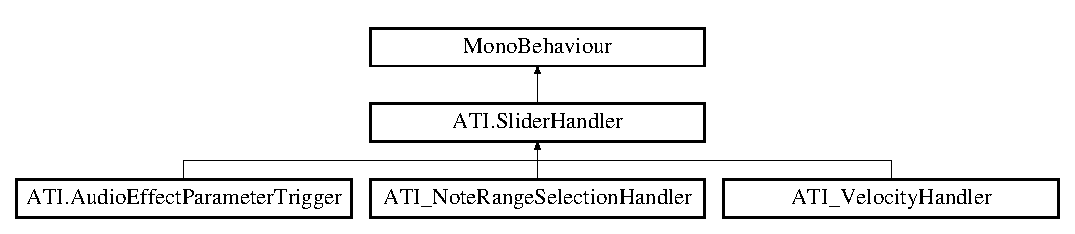
\includegraphics[height=2.692308cm]{class_a_t_i_1_1_slider_handler}
\end{center}
\end{figure}
\subsection*{Public Member Functions}
\begin{DoxyCompactItemize}
\item 
void \hyperlink{class_a_t_i_1_1_slider_handler_ad7cd02a45170b1a4af432d1ccc2490ea}{Start} ()
\item 
int \hyperlink{class_a_t_i_1_1_slider_handler_ab6c7a9d82c98d87ebbe45c8a032dbd29}{Get\+Slider\+Index} (Slider a\+Slider)
\item 
void \hyperlink{class_a_t_i_1_1_slider_handler_a0ef4eeb2a91b744eaaf2453856aded60}{Handle\+Drag} (Slider a\+Slider, \hyperlink{class_a_t_i_ac4c6056a99cbd16ff0d292d33b038b9b}{Slider\+Type} a\+Slider\+Type)
\item 
void \hyperlink{class_a_t_i_1_1_slider_handler_ada65f41ef84f50737cece7be16c548f9}{Handle\+Drag\+End} (Slider a\+Slider, \hyperlink{class_a_t_i_ac4c6056a99cbd16ff0d292d33b038b9b}{Slider\+Type} a\+Slider\+Type)
\end{DoxyCompactItemize}
\subsection*{Protected Member Functions}
\begin{DoxyCompactItemize}
\item 
virtual void \hyperlink{class_a_t_i_1_1_slider_handler_ac82219a0a69f17025d9484f9e45cca80}{Handle\+Musical\+Typing\+Key\+Velocity\+Change} (int a\+Slider\+Index)
\item 
virtual void \hyperlink{class_a_t_i_1_1_slider_handler_a710b59b6e8bf059af76477a930572d9e}{Handle\+Lowest\+Random\+Velocity\+Change} (bool a\+End\+Drag)
\item 
virtual void \hyperlink{class_a_t_i_1_1_slider_handler_a827fab40da8ee6e777cbed4b5a9ae712}{Handle\+Highest\+Random\+Velocity\+Change} (bool a\+End\+Drag)
\item 
virtual void \hyperlink{class_a_t_i_1_1_slider_handler_a4d3915be92feddd4c45027a71c3a338c}{Handle\+Note\+Range\+Change} (bool a\+End\+Drag)
\item 
virtual void \hyperlink{class_a_t_i_1_1_slider_handler_a51fd8e687677af70535a9332ded83d3b}{Send\+Slider\+Change\+To\+Handler} ()
\end{DoxyCompactItemize}
\subsection*{Protected Attributes}
\begin{DoxyCompactItemize}
\item 
int \hyperlink{class_a_t_i_1_1_slider_handler_ac762fad2fb523da79188668dde4488ec}{m\+Num\+Sliders}
\item 
Slider \mbox{[}$\,$\mbox{]} \hyperlink{class_a_t_i_1_1_slider_handler_a038a487fbd701cb786e77c210830be76}{m\+Sliders}
\item 
\hyperlink{class_a_t_i_1_1_slider_trigger}{Slider\+Trigger} \mbox{[}$\,$\mbox{]} \hyperlink{class_a_t_i_1_1_slider_handler_a20208bc52a906cf87aa9df8e5fb2c636}{m\+Slider\+Triggers}
\item 
\hyperlink{class_virtual_instrument_manager}{Virtual\+Instrument\+Manager} \hyperlink{class_a_t_i_1_1_slider_handler_a5d19b4fb92b71c25a667defdda60213f}{m\+V\+IM} = null
\end{DoxyCompactItemize}


\subsection{Detailed Description}


Definition at line 124 of file A\+T\+I.\+cs.



\subsection{Member Function Documentation}
\mbox{\Hypertarget{class_a_t_i_1_1_slider_handler_ab6c7a9d82c98d87ebbe45c8a032dbd29}\label{class_a_t_i_1_1_slider_handler_ab6c7a9d82c98d87ebbe45c8a032dbd29}} 
\index{A\+T\+I\+::\+Slider\+Handler@{A\+T\+I\+::\+Slider\+Handler}!Get\+Slider\+Index@{Get\+Slider\+Index}}
\index{Get\+Slider\+Index@{Get\+Slider\+Index}!A\+T\+I\+::\+Slider\+Handler@{A\+T\+I\+::\+Slider\+Handler}}
\subsubsection{\texorpdfstring{Get\+Slider\+Index()}{GetSliderIndex()}}
{\footnotesize\ttfamily int A\+T\+I.\+Slider\+Handler.\+Get\+Slider\+Index (\begin{DoxyParamCaption}\item[{Slider}]{a\+Slider }\end{DoxyParamCaption})}



Definition at line 150 of file A\+T\+I.\+cs.


\begin{DoxyCode}
151         \{
152             \textcolor{keywordflow}{if}( \hyperlink{class_a_t_i_1_1_slider_handler_a038a487fbd701cb786e77c210830be76}{mSliders} != null )
153             \{
154                 \textcolor{comment}{// If the slider is in the container, then return its index.}
155                 \textcolor{keywordflow}{for}( \textcolor{keywordtype}{int} i = 0; i < \hyperlink{class_a_t_i_1_1_slider_handler_ac762fad2fb523da79188668dde4488ec}{mNumSliders}; i++ )
156                 \{
157                     \textcolor{keywordflow}{if}( \hyperlink{class_a_t_i_1_1_slider_handler_a038a487fbd701cb786e77c210830be76}{mSliders}[i] == aSlider )
158                     \{
159                         \textcolor{keywordflow}{return} i;
160                     \}
161                 \}
162             \}
163 
164             \textcolor{comment}{// If the slider is not in the container, then something has gone wrong.}
165             \textcolor{keywordflow}{else}
166             \{
167                 Assert.IsTrue( \textcolor{keyword}{false}, \textcolor{stringliteral}{"Slider Handler tried to handle a slider event, but the handler was
       uninitialized!"} );
168             \}
169 
170             \textcolor{keywordflow}{return} -1;
171 
172         \}
\end{DoxyCode}
\mbox{\Hypertarget{class_a_t_i_1_1_slider_handler_a0ef4eeb2a91b744eaaf2453856aded60}\label{class_a_t_i_1_1_slider_handler_a0ef4eeb2a91b744eaaf2453856aded60}} 
\index{A\+T\+I\+::\+Slider\+Handler@{A\+T\+I\+::\+Slider\+Handler}!Handle\+Drag@{Handle\+Drag}}
\index{Handle\+Drag@{Handle\+Drag}!A\+T\+I\+::\+Slider\+Handler@{A\+T\+I\+::\+Slider\+Handler}}
\subsubsection{\texorpdfstring{Handle\+Drag()}{HandleDrag()}}
{\footnotesize\ttfamily void A\+T\+I.\+Slider\+Handler.\+Handle\+Drag (\begin{DoxyParamCaption}\item[{Slider}]{a\+Slider,  }\item[{\hyperlink{class_a_t_i_ac4c6056a99cbd16ff0d292d33b038b9b}{Slider\+Type}}]{a\+Slider\+Type }\end{DoxyParamCaption})}



Definition at line 181 of file A\+T\+I.\+cs.



Referenced by A\+T\+I.\+Slider\+Trigger.\+On\+Drag().


\begin{DoxyCode}
182         \{
183             \textcolor{comment}{// Call the appropriate function for the slider type.}
184             \textcolor{keywordflow}{switch}( aSliderType )
185             \{
186                 \textcolor{keywordflow}{case} \hyperlink{class_a_t_i_ac4c6056a99cbd16ff0d292d33b038b9b}{SliderType}.MusicalTypingKeyVelocity:
187                     \hyperlink{class_a_t_i_1_1_slider_handler_ac82219a0a69f17025d9484f9e45cca80}{HandleMusicalTypingKeyVelocityChange}( 
      \hyperlink{class_a_t_i_1_1_slider_handler_ab6c7a9d82c98d87ebbe45c8a032dbd29}{GetSliderIndex}( aSlider ) );
188                     \textcolor{keywordflow}{break};
189                 \textcolor{keywordflow}{case} \hyperlink{class_a_t_i_ac4c6056a99cbd16ff0d292d33b038b9b}{SliderType}.LowestRandomKeyVelocity:
190                     \hyperlink{class_a_t_i_1_1_slider_handler_a710b59b6e8bf059af76477a930572d9e}{HandleLowestRandomVelocityChange}( \textcolor{keyword}{false} );
191                     \textcolor{keywordflow}{break};
192                 \textcolor{keywordflow}{case} \hyperlink{class_a_t_i_ac4c6056a99cbd16ff0d292d33b038b9b}{SliderType}.HighestRandomKeyVelocity:
193                     \hyperlink{class_a_t_i_1_1_slider_handler_a827fab40da8ee6e777cbed4b5a9ae712}{HandleHighestRandomVelocityChange}( \textcolor{keyword}{false} );
194                     \textcolor{keywordflow}{break};
195                 \textcolor{keywordflow}{case} \hyperlink{class_a_t_i_ac4c6056a99cbd16ff0d292d33b038b9b}{SliderType}.NoteRange:
196                     \hyperlink{class_a_t_i_1_1_slider_handler_a4d3915be92feddd4c45027a71c3a338c}{HandleNoteRangeChange}( \textcolor{keyword}{false} );
197                     \textcolor{keywordflow}{break};
198                 \textcolor{keywordflow}{case} \hyperlink{class_a_t_i_ac4c6056a99cbd16ff0d292d33b038b9b}{SliderType}.AudioEffectParameter:
199                     \hyperlink{class_a_t_i_1_1_slider_handler_a51fd8e687677af70535a9332ded83d3b}{SendSliderChangeToHandler}();
200                     \textcolor{keywordflow}{break};
201                 \textcolor{keywordflow}{default}:
202                     \textcolor{keywordflow}{break};
203             \}
204         \}
\end{DoxyCode}
\mbox{\Hypertarget{class_a_t_i_1_1_slider_handler_ada65f41ef84f50737cece7be16c548f9}\label{class_a_t_i_1_1_slider_handler_ada65f41ef84f50737cece7be16c548f9}} 
\index{A\+T\+I\+::\+Slider\+Handler@{A\+T\+I\+::\+Slider\+Handler}!Handle\+Drag\+End@{Handle\+Drag\+End}}
\index{Handle\+Drag\+End@{Handle\+Drag\+End}!A\+T\+I\+::\+Slider\+Handler@{A\+T\+I\+::\+Slider\+Handler}}
\subsubsection{\texorpdfstring{Handle\+Drag\+End()}{HandleDragEnd()}}
{\footnotesize\ttfamily void A\+T\+I.\+Slider\+Handler.\+Handle\+Drag\+End (\begin{DoxyParamCaption}\item[{Slider}]{a\+Slider,  }\item[{\hyperlink{class_a_t_i_ac4c6056a99cbd16ff0d292d33b038b9b}{Slider\+Type}}]{a\+Slider\+Type }\end{DoxyParamCaption})}



Definition at line 209 of file A\+T\+I.\+cs.



Referenced by A\+T\+I.\+Slider\+Trigger.\+On\+End\+Drag().


\begin{DoxyCode}
210         \{
211             \textcolor{comment}{// Call the appropriate function for the slider type.}
212             \textcolor{keywordflow}{switch}( aSliderType )
213             \{
214                 \textcolor{keywordflow}{case} \hyperlink{class_a_t_i_ac4c6056a99cbd16ff0d292d33b038b9b}{SliderType}.MusicalTypingKeyVelocity:
215                     \hyperlink{class_a_t_i_1_1_slider_handler_ac82219a0a69f17025d9484f9e45cca80}{HandleMusicalTypingKeyVelocityChange}( 
      \hyperlink{class_a_t_i_1_1_slider_handler_ab6c7a9d82c98d87ebbe45c8a032dbd29}{GetSliderIndex}( aSlider ) );
216                     \textcolor{keywordflow}{break};
217                 \textcolor{keywordflow}{case} \hyperlink{class_a_t_i_ac4c6056a99cbd16ff0d292d33b038b9b}{SliderType}.LowestRandomKeyVelocity:
218                     \hyperlink{class_a_t_i_1_1_slider_handler_a710b59b6e8bf059af76477a930572d9e}{HandleLowestRandomVelocityChange}( \textcolor{keyword}{true} );
219                     \textcolor{keywordflow}{break};
220                 \textcolor{keywordflow}{case} \hyperlink{class_a_t_i_ac4c6056a99cbd16ff0d292d33b038b9b}{SliderType}.HighestRandomKeyVelocity:
221                     \hyperlink{class_a_t_i_1_1_slider_handler_a827fab40da8ee6e777cbed4b5a9ae712}{HandleHighestRandomVelocityChange}( \textcolor{keyword}{true} );
222                     \textcolor{keywordflow}{break};
223                 \textcolor{keywordflow}{case} \hyperlink{class_a_t_i_ac4c6056a99cbd16ff0d292d33b038b9b}{SliderType}.NoteRange:
224                     \hyperlink{class_a_t_i_1_1_slider_handler_a4d3915be92feddd4c45027a71c3a338c}{HandleNoteRangeChange}( \textcolor{keyword}{true} );
225                     \textcolor{keywordflow}{break};
226                 \textcolor{keywordflow}{case} \hyperlink{class_a_t_i_ac4c6056a99cbd16ff0d292d33b038b9b}{SliderType}.AudioEffectParameter:
227                     \hyperlink{class_a_t_i_1_1_slider_handler_a51fd8e687677af70535a9332ded83d3b}{SendSliderChangeToHandler}();
228                     \textcolor{keywordflow}{break};
229                 \textcolor{keywordflow}{default}:
230                     \textcolor{keywordflow}{break};
231             \}
232         \}
\end{DoxyCode}
\mbox{\Hypertarget{class_a_t_i_1_1_slider_handler_a827fab40da8ee6e777cbed4b5a9ae712}\label{class_a_t_i_1_1_slider_handler_a827fab40da8ee6e777cbed4b5a9ae712}} 
\index{A\+T\+I\+::\+Slider\+Handler@{A\+T\+I\+::\+Slider\+Handler}!Handle\+Highest\+Random\+Velocity\+Change@{Handle\+Highest\+Random\+Velocity\+Change}}
\index{Handle\+Highest\+Random\+Velocity\+Change@{Handle\+Highest\+Random\+Velocity\+Change}!A\+T\+I\+::\+Slider\+Handler@{A\+T\+I\+::\+Slider\+Handler}}
\subsubsection{\texorpdfstring{Handle\+Highest\+Random\+Velocity\+Change()}{HandleHighestRandomVelocityChange()}}
{\footnotesize\ttfamily virtual void A\+T\+I.\+Slider\+Handler.\+Handle\+Highest\+Random\+Velocity\+Change (\begin{DoxyParamCaption}\item[{bool}]{a\+End\+Drag }\end{DoxyParamCaption})\hspace{0.3cm}{\ttfamily [protected]}, {\ttfamily [virtual]}}



Reimplemented in \hyperlink{class_a_t_i___velocity_handler_a6e1fd3ceb35873a09e138bebd0c323fd}{A\+T\+I\+\_\+\+Velocity\+Handler}.



Definition at line 239 of file A\+T\+I.\+cs.


\begin{DoxyCode}
239 \{ \}
\end{DoxyCode}
\mbox{\Hypertarget{class_a_t_i_1_1_slider_handler_a710b59b6e8bf059af76477a930572d9e}\label{class_a_t_i_1_1_slider_handler_a710b59b6e8bf059af76477a930572d9e}} 
\index{A\+T\+I\+::\+Slider\+Handler@{A\+T\+I\+::\+Slider\+Handler}!Handle\+Lowest\+Random\+Velocity\+Change@{Handle\+Lowest\+Random\+Velocity\+Change}}
\index{Handle\+Lowest\+Random\+Velocity\+Change@{Handle\+Lowest\+Random\+Velocity\+Change}!A\+T\+I\+::\+Slider\+Handler@{A\+T\+I\+::\+Slider\+Handler}}
\subsubsection{\texorpdfstring{Handle\+Lowest\+Random\+Velocity\+Change()}{HandleLowestRandomVelocityChange()}}
{\footnotesize\ttfamily virtual void A\+T\+I.\+Slider\+Handler.\+Handle\+Lowest\+Random\+Velocity\+Change (\begin{DoxyParamCaption}\item[{bool}]{a\+End\+Drag }\end{DoxyParamCaption})\hspace{0.3cm}{\ttfamily [protected]}, {\ttfamily [virtual]}}



Reimplemented in \hyperlink{class_a_t_i___velocity_handler_a17b6e0de9e45dfb9dba1ea4f2c0a122c}{A\+T\+I\+\_\+\+Velocity\+Handler}.



Definition at line 238 of file A\+T\+I.\+cs.


\begin{DoxyCode}
238 \{ \}
\end{DoxyCode}
\mbox{\Hypertarget{class_a_t_i_1_1_slider_handler_ac82219a0a69f17025d9484f9e45cca80}\label{class_a_t_i_1_1_slider_handler_ac82219a0a69f17025d9484f9e45cca80}} 
\index{A\+T\+I\+::\+Slider\+Handler@{A\+T\+I\+::\+Slider\+Handler}!Handle\+Musical\+Typing\+Key\+Velocity\+Change@{Handle\+Musical\+Typing\+Key\+Velocity\+Change}}
\index{Handle\+Musical\+Typing\+Key\+Velocity\+Change@{Handle\+Musical\+Typing\+Key\+Velocity\+Change}!A\+T\+I\+::\+Slider\+Handler@{A\+T\+I\+::\+Slider\+Handler}}
\subsubsection{\texorpdfstring{Handle\+Musical\+Typing\+Key\+Velocity\+Change()}{HandleMusicalTypingKeyVelocityChange()}}
{\footnotesize\ttfamily virtual void A\+T\+I.\+Slider\+Handler.\+Handle\+Musical\+Typing\+Key\+Velocity\+Change (\begin{DoxyParamCaption}\item[{int}]{a\+Slider\+Index }\end{DoxyParamCaption})\hspace{0.3cm}{\ttfamily [protected]}, {\ttfamily [virtual]}}



Reimplemented in \hyperlink{class_a_t_i___velocity_handler_a5b00635239f4f10aaefc5898a8f1b975}{A\+T\+I\+\_\+\+Velocity\+Handler}.



Definition at line 237 of file A\+T\+I.\+cs.


\begin{DoxyCode}
237 \{ \}
\end{DoxyCode}
\mbox{\Hypertarget{class_a_t_i_1_1_slider_handler_a4d3915be92feddd4c45027a71c3a338c}\label{class_a_t_i_1_1_slider_handler_a4d3915be92feddd4c45027a71c3a338c}} 
\index{A\+T\+I\+::\+Slider\+Handler@{A\+T\+I\+::\+Slider\+Handler}!Handle\+Note\+Range\+Change@{Handle\+Note\+Range\+Change}}
\index{Handle\+Note\+Range\+Change@{Handle\+Note\+Range\+Change}!A\+T\+I\+::\+Slider\+Handler@{A\+T\+I\+::\+Slider\+Handler}}
\subsubsection{\texorpdfstring{Handle\+Note\+Range\+Change()}{HandleNoteRangeChange()}}
{\footnotesize\ttfamily virtual void A\+T\+I.\+Slider\+Handler.\+Handle\+Note\+Range\+Change (\begin{DoxyParamCaption}\item[{bool}]{a\+End\+Drag }\end{DoxyParamCaption})\hspace{0.3cm}{\ttfamily [protected]}, {\ttfamily [virtual]}}



Reimplemented in \hyperlink{class_a_t_i___note_range_selection_handler_a87e90cac12626a0cb547d6e40c6e8260}{A\+T\+I\+\_\+\+Note\+Range\+Selection\+Handler}.



Definition at line 240 of file A\+T\+I.\+cs.


\begin{DoxyCode}
240 \{ \}
\end{DoxyCode}
\mbox{\Hypertarget{class_a_t_i_1_1_slider_handler_a51fd8e687677af70535a9332ded83d3b}\label{class_a_t_i_1_1_slider_handler_a51fd8e687677af70535a9332ded83d3b}} 
\index{A\+T\+I\+::\+Slider\+Handler@{A\+T\+I\+::\+Slider\+Handler}!Send\+Slider\+Change\+To\+Handler@{Send\+Slider\+Change\+To\+Handler}}
\index{Send\+Slider\+Change\+To\+Handler@{Send\+Slider\+Change\+To\+Handler}!A\+T\+I\+::\+Slider\+Handler@{A\+T\+I\+::\+Slider\+Handler}}
\subsubsection{\texorpdfstring{Send\+Slider\+Change\+To\+Handler()}{SendSliderChangeToHandler()}}
{\footnotesize\ttfamily virtual void A\+T\+I.\+Slider\+Handler.\+Send\+Slider\+Change\+To\+Handler (\begin{DoxyParamCaption}{ }\end{DoxyParamCaption})\hspace{0.3cm}{\ttfamily [protected]}, {\ttfamily [virtual]}}



Reimplemented in \hyperlink{class_a_t_i_1_1_audio_effect_parameter_trigger_ad1dde7a7b8ca7db2766b4941ef826e76}{A\+T\+I.\+Audio\+Effect\+Parameter\+Trigger}.



Definition at line 241 of file A\+T\+I.\+cs.


\begin{DoxyCode}
241 \{ \}
\end{DoxyCode}
\mbox{\Hypertarget{class_a_t_i_1_1_slider_handler_ad7cd02a45170b1a4af432d1ccc2490ea}\label{class_a_t_i_1_1_slider_handler_ad7cd02a45170b1a4af432d1ccc2490ea}} 
\index{A\+T\+I\+::\+Slider\+Handler@{A\+T\+I\+::\+Slider\+Handler}!Start@{Start}}
\index{Start@{Start}!A\+T\+I\+::\+Slider\+Handler@{A\+T\+I\+::\+Slider\+Handler}}
\subsubsection{\texorpdfstring{Start()}{Start()}}
{\footnotesize\ttfamily void A\+T\+I.\+Slider\+Handler.\+Start (\begin{DoxyParamCaption}{ }\end{DoxyParamCaption})}



Definition at line 137 of file A\+T\+I.\+cs.


\begin{DoxyCode}
138         \{
139             \textcolor{comment}{// Get the virtual instrument manager.}
140             \hyperlink{class_a_t_i_1_1_slider_handler_a5d19b4fb92b71c25a667defdda60213f}{mVIM} = GameObject.Find( \textcolor{stringliteral}{"VirtualInstrumentManager"} ).GetComponent<
      \hyperlink{class_virtual_instrument_manager}{VirtualInstrumentManager}>();
141         \}
\end{DoxyCode}


\subsection{Member Data Documentation}
\mbox{\Hypertarget{class_a_t_i_1_1_slider_handler_ac762fad2fb523da79188668dde4488ec}\label{class_a_t_i_1_1_slider_handler_ac762fad2fb523da79188668dde4488ec}} 
\index{A\+T\+I\+::\+Slider\+Handler@{A\+T\+I\+::\+Slider\+Handler}!m\+Num\+Sliders@{m\+Num\+Sliders}}
\index{m\+Num\+Sliders@{m\+Num\+Sliders}!A\+T\+I\+::\+Slider\+Handler@{A\+T\+I\+::\+Slider\+Handler}}
\subsubsection{\texorpdfstring{m\+Num\+Sliders}{mNumSliders}}
{\footnotesize\ttfamily int A\+T\+I.\+Slider\+Handler.\+m\+Num\+Sliders\hspace{0.3cm}{\ttfamily [protected]}}



Definition at line 129 of file A\+T\+I.\+cs.



Referenced by A\+T\+I\+\_\+\+Velocity\+Handler.\+Start().

\mbox{\Hypertarget{class_a_t_i_1_1_slider_handler_a038a487fbd701cb786e77c210830be76}\label{class_a_t_i_1_1_slider_handler_a038a487fbd701cb786e77c210830be76}} 
\index{A\+T\+I\+::\+Slider\+Handler@{A\+T\+I\+::\+Slider\+Handler}!m\+Sliders@{m\+Sliders}}
\index{m\+Sliders@{m\+Sliders}!A\+T\+I\+::\+Slider\+Handler@{A\+T\+I\+::\+Slider\+Handler}}
\subsubsection{\texorpdfstring{m\+Sliders}{mSliders}}
{\footnotesize\ttfamily Slider \mbox{[}$\,$\mbox{]} A\+T\+I.\+Slider\+Handler.\+m\+Sliders\hspace{0.3cm}{\ttfamily [protected]}}



Definition at line 130 of file A\+T\+I.\+cs.



Referenced by A\+T\+I\+\_\+\+Note\+Range\+Selection\+Handler.\+Handle\+Instrument\+Loaded(), A\+T\+I\+\_\+\+Velocity\+Handler.\+Handle\+Musical\+Typing\+Key\+Velocity\+Change(), A\+T\+I\+\_\+\+Note\+Range\+Selection\+Handler.\+Handle\+Note\+Range\+Change(), A\+T\+I\+\_\+\+Note\+Range\+Selection\+Handler.\+Start(), and A\+T\+I\+\_\+\+Velocity\+Handler.\+Start().

\mbox{\Hypertarget{class_a_t_i_1_1_slider_handler_a20208bc52a906cf87aa9df8e5fb2c636}\label{class_a_t_i_1_1_slider_handler_a20208bc52a906cf87aa9df8e5fb2c636}} 
\index{A\+T\+I\+::\+Slider\+Handler@{A\+T\+I\+::\+Slider\+Handler}!m\+Slider\+Triggers@{m\+Slider\+Triggers}}
\index{m\+Slider\+Triggers@{m\+Slider\+Triggers}!A\+T\+I\+::\+Slider\+Handler@{A\+T\+I\+::\+Slider\+Handler}}
\subsubsection{\texorpdfstring{m\+Slider\+Triggers}{mSliderTriggers}}
{\footnotesize\ttfamily \hyperlink{class_a_t_i_1_1_slider_trigger}{Slider\+Trigger} \mbox{[}$\,$\mbox{]} A\+T\+I.\+Slider\+Handler.\+m\+Slider\+Triggers\hspace{0.3cm}{\ttfamily [protected]}}



Definition at line 131 of file A\+T\+I.\+cs.



Referenced by A\+T\+I\+\_\+\+Velocity\+Handler.\+Start().

\mbox{\Hypertarget{class_a_t_i_1_1_slider_handler_a5d19b4fb92b71c25a667defdda60213f}\label{class_a_t_i_1_1_slider_handler_a5d19b4fb92b71c25a667defdda60213f}} 
\index{A\+T\+I\+::\+Slider\+Handler@{A\+T\+I\+::\+Slider\+Handler}!m\+V\+IM@{m\+V\+IM}}
\index{m\+V\+IM@{m\+V\+IM}!A\+T\+I\+::\+Slider\+Handler@{A\+T\+I\+::\+Slider\+Handler}}
\subsubsection{\texorpdfstring{m\+V\+IM}{mVIM}}
{\footnotesize\ttfamily \hyperlink{class_virtual_instrument_manager}{Virtual\+Instrument\+Manager} A\+T\+I.\+Slider\+Handler.\+m\+V\+IM = null\hspace{0.3cm}{\ttfamily [protected]}}



Definition at line 132 of file A\+T\+I.\+cs.



Referenced by A\+T\+I\+\_\+\+Note\+Range\+Selection\+Handler.\+Handle\+Instrument\+Loaded(), A\+T\+I\+\_\+\+Velocity\+Handler.\+Handle\+Musical\+Typing\+Key\+Velocity\+Change(), A\+T\+I\+\_\+\+Note\+Range\+Selection\+Handler.\+Handle\+Note\+Range\+Change(), A\+T\+I\+\_\+\+Velocity\+Handler.\+Randomize\+Key\+Velocities(), and A\+T\+I\+\_\+\+Note\+Range\+Selection\+Handler.\+Start().



The documentation for this class was generated from the following file\+:\begin{DoxyCompactItemize}
\item 
D\+:/\+Documents/\+School Documents/2017\+Spring/\+E\+E\+C\+S542/\+V\+R\+Piano\+Project/\+Assets/\+Scripts/\+Audio/\+Testing/\hyperlink{_a_t_i_8cs}{A\+T\+I.\+cs}\end{DoxyCompactItemize}

\hypertarget{class_a_t_i_1_1_slider_trigger}{}\section{A\+T\+I.\+Slider\+Trigger Class Reference}
\label{class_a_t_i_1_1_slider_trigger}\index{A\+T\+I.\+Slider\+Trigger@{A\+T\+I.\+Slider\+Trigger}}
Inheritance diagram for A\+T\+I.\+Slider\+Trigger\+:\begin{figure}[H]
\begin{center}
\leavevmode
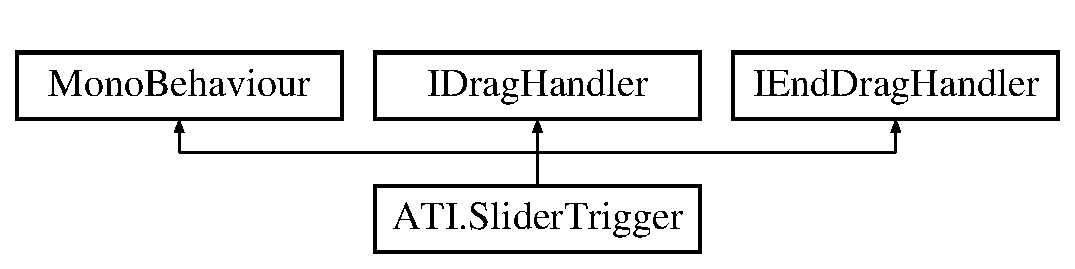
\includegraphics[height=2.000000cm]{class_a_t_i_1_1_slider_trigger}
\end{center}
\end{figure}
\subsection*{Public Member Functions}
\begin{DoxyCompactItemize}
\item 
void \hyperlink{class_a_t_i_1_1_slider_trigger_a03b00593630437fbf23973564ebd35ec}{Awake} ()
\item 
void \hyperlink{class_a_t_i_1_1_slider_trigger_a258f79d013266d0c82a5382525adcdef}{Set\+Handler} (\hyperlink{class_a_t_i_1_1_slider_handler}{Slider\+Handler} a\+Handler)
\item 
void \hyperlink{class_a_t_i_1_1_slider_trigger_a90347192aede3444d468ed2ab0d97f6c}{Set\+Type} (\hyperlink{class_a_t_i_ac4c6056a99cbd16ff0d292d33b038b9b}{Slider\+Type} a\+Type)
\item 
void \hyperlink{class_a_t_i_1_1_slider_trigger_abed7a842d506b1f727b7e2b3cbb58aae}{On\+Drag} (Pointer\+Event\+Data a\+Event\+Data)
\item 
void \hyperlink{class_a_t_i_1_1_slider_trigger_ae58a83edce79a49d1fd21317c7536b48}{On\+End\+Drag} (Pointer\+Event\+Data a\+Event\+Data)
\end{DoxyCompactItemize}
\subsection*{Private Attributes}
\begin{DoxyCompactItemize}
\item 
Slider \hyperlink{class_a_t_i_1_1_slider_trigger_adb4a609592234cac1451eeeb2d394740}{m\+Slider}
\item 
\hyperlink{class_a_t_i_1_1_slider_handler}{Slider\+Handler} \hyperlink{class_a_t_i_1_1_slider_trigger_ab2c5ecc1828e1618dc7966aa815fdaba}{m\+Handler}
\item 
\hyperlink{class_a_t_i_ac4c6056a99cbd16ff0d292d33b038b9b}{Slider\+Type} \hyperlink{class_a_t_i_1_1_slider_trigger_a62a01bc9c41be54f58bd77664181fd5d}{m\+Slider\+Type}
\end{DoxyCompactItemize}


\subsection{Detailed Description}


Definition at line 62 of file A\+T\+I.\+cs.



\subsection{Member Function Documentation}
\mbox{\Hypertarget{class_a_t_i_1_1_slider_trigger_a03b00593630437fbf23973564ebd35ec}\label{class_a_t_i_1_1_slider_trigger_a03b00593630437fbf23973564ebd35ec}} 
\index{A\+T\+I\+::\+Slider\+Trigger@{A\+T\+I\+::\+Slider\+Trigger}!Awake@{Awake}}
\index{Awake@{Awake}!A\+T\+I\+::\+Slider\+Trigger@{A\+T\+I\+::\+Slider\+Trigger}}
\subsubsection{\texorpdfstring{Awake()}{Awake()}}
{\footnotesize\ttfamily void A\+T\+I.\+Slider\+Trigger.\+Awake (\begin{DoxyParamCaption}{ }\end{DoxyParamCaption})}



Definition at line 75 of file A\+T\+I.\+cs.


\begin{DoxyCode}
76         \{
77             \hyperlink{class_a_t_i_1_1_slider_trigger_adb4a609592234cac1451eeeb2d394740}{mSlider} = gameObject.transform.GetComponent<Slider>();
78             \hyperlink{class_a_t_i_1_1_slider_trigger_ab2c5ecc1828e1618dc7966aa815fdaba}{mHandler} = null;
79             \hyperlink{class_a_t_i_1_1_slider_trigger_a62a01bc9c41be54f58bd77664181fd5d}{mSliderType} = \hyperlink{class_a_t_i_ac4c6056a99cbd16ff0d292d33b038b9b}{SliderType}.Uninitialized;
80         \}
\end{DoxyCode}
\mbox{\Hypertarget{class_a_t_i_1_1_slider_trigger_abed7a842d506b1f727b7e2b3cbb58aae}\label{class_a_t_i_1_1_slider_trigger_abed7a842d506b1f727b7e2b3cbb58aae}} 
\index{A\+T\+I\+::\+Slider\+Trigger@{A\+T\+I\+::\+Slider\+Trigger}!On\+Drag@{On\+Drag}}
\index{On\+Drag@{On\+Drag}!A\+T\+I\+::\+Slider\+Trigger@{A\+T\+I\+::\+Slider\+Trigger}}
\subsubsection{\texorpdfstring{On\+Drag()}{OnDrag()}}
{\footnotesize\ttfamily void A\+T\+I.\+Slider\+Trigger.\+On\+Drag (\begin{DoxyParamCaption}\item[{Pointer\+Event\+Data}]{a\+Event\+Data }\end{DoxyParamCaption})}



Definition at line 106 of file A\+T\+I.\+cs.



References A\+T\+I.\+Slider\+Handler.\+Handle\+Drag().


\begin{DoxyCode}
107         \{
108             \textcolor{keywordflow}{if}( aEventData.dragging )
109             \{
110                 \hyperlink{class_a_t_i_1_1_slider_trigger_ab2c5ecc1828e1618dc7966aa815fdaba}{mHandler}.\hyperlink{class_a_t_i_1_1_slider_handler_a0ef4eeb2a91b744eaaf2453856aded60}{HandleDrag}( \hyperlink{class_a_t_i_1_1_slider_trigger_adb4a609592234cac1451eeeb2d394740}{mSlider}, 
      \hyperlink{class_a_t_i_1_1_slider_trigger_a62a01bc9c41be54f58bd77664181fd5d}{mSliderType} );
111             \}
112         \}
\end{DoxyCode}
\mbox{\Hypertarget{class_a_t_i_1_1_slider_trigger_ae58a83edce79a49d1fd21317c7536b48}\label{class_a_t_i_1_1_slider_trigger_ae58a83edce79a49d1fd21317c7536b48}} 
\index{A\+T\+I\+::\+Slider\+Trigger@{A\+T\+I\+::\+Slider\+Trigger}!On\+End\+Drag@{On\+End\+Drag}}
\index{On\+End\+Drag@{On\+End\+Drag}!A\+T\+I\+::\+Slider\+Trigger@{A\+T\+I\+::\+Slider\+Trigger}}
\subsubsection{\texorpdfstring{On\+End\+Drag()}{OnEndDrag()}}
{\footnotesize\ttfamily void A\+T\+I.\+Slider\+Trigger.\+On\+End\+Drag (\begin{DoxyParamCaption}\item[{Pointer\+Event\+Data}]{a\+Event\+Data }\end{DoxyParamCaption})}



Definition at line 116 of file A\+T\+I.\+cs.



References A\+T\+I.\+Slider\+Handler.\+Handle\+Drag\+End().


\begin{DoxyCode}
117         \{
118             \hyperlink{class_a_t_i_1_1_slider_trigger_ab2c5ecc1828e1618dc7966aa815fdaba}{mHandler}.\hyperlink{class_a_t_i_1_1_slider_handler_ada65f41ef84f50737cece7be16c548f9}{HandleDragEnd}( \hyperlink{class_a_t_i_1_1_slider_trigger_adb4a609592234cac1451eeeb2d394740}{mSlider}, 
      \hyperlink{class_a_t_i_1_1_slider_trigger_a62a01bc9c41be54f58bd77664181fd5d}{mSliderType} );
119         \}
\end{DoxyCode}
\mbox{\Hypertarget{class_a_t_i_1_1_slider_trigger_a258f79d013266d0c82a5382525adcdef}\label{class_a_t_i_1_1_slider_trigger_a258f79d013266d0c82a5382525adcdef}} 
\index{A\+T\+I\+::\+Slider\+Trigger@{A\+T\+I\+::\+Slider\+Trigger}!Set\+Handler@{Set\+Handler}}
\index{Set\+Handler@{Set\+Handler}!A\+T\+I\+::\+Slider\+Trigger@{A\+T\+I\+::\+Slider\+Trigger}}
\subsubsection{\texorpdfstring{Set\+Handler()}{SetHandler()}}
{\footnotesize\ttfamily void A\+T\+I.\+Slider\+Trigger.\+Set\+Handler (\begin{DoxyParamCaption}\item[{\hyperlink{class_a_t_i_1_1_slider_handler}{Slider\+Handler}}]{a\+Handler }\end{DoxyParamCaption})}



Definition at line 88 of file A\+T\+I.\+cs.



Referenced by A\+T\+I.\+Audio\+Effect\+Parameter\+Trigger.\+Awake(), A\+T\+I\+\_\+\+Note\+Range\+Selection\+Handler.\+Start(), and A\+T\+I\+\_\+\+Velocity\+Handler.\+Start().


\begin{DoxyCode}
89         \{
90             \hyperlink{class_a_t_i_1_1_slider_trigger_ab2c5ecc1828e1618dc7966aa815fdaba}{mHandler} = aHandler;
91         \}
\end{DoxyCode}
\mbox{\Hypertarget{class_a_t_i_1_1_slider_trigger_a90347192aede3444d468ed2ab0d97f6c}\label{class_a_t_i_1_1_slider_trigger_a90347192aede3444d468ed2ab0d97f6c}} 
\index{A\+T\+I\+::\+Slider\+Trigger@{A\+T\+I\+::\+Slider\+Trigger}!Set\+Type@{Set\+Type}}
\index{Set\+Type@{Set\+Type}!A\+T\+I\+::\+Slider\+Trigger@{A\+T\+I\+::\+Slider\+Trigger}}
\subsubsection{\texorpdfstring{Set\+Type()}{SetType()}}
{\footnotesize\ttfamily void A\+T\+I.\+Slider\+Trigger.\+Set\+Type (\begin{DoxyParamCaption}\item[{\hyperlink{class_a_t_i_ac4c6056a99cbd16ff0d292d33b038b9b}{Slider\+Type}}]{a\+Type }\end{DoxyParamCaption})}



Definition at line 95 of file A\+T\+I.\+cs.



Referenced by A\+T\+I\+\_\+\+Velocity\+Handler.\+Start().


\begin{DoxyCode}
96         \{
97             \hyperlink{class_a_t_i_1_1_slider_trigger_a62a01bc9c41be54f58bd77664181fd5d}{mSliderType} = aType;
98         \}
\end{DoxyCode}


\subsection{Member Data Documentation}
\mbox{\Hypertarget{class_a_t_i_1_1_slider_trigger_ab2c5ecc1828e1618dc7966aa815fdaba}\label{class_a_t_i_1_1_slider_trigger_ab2c5ecc1828e1618dc7966aa815fdaba}} 
\index{A\+T\+I\+::\+Slider\+Trigger@{A\+T\+I\+::\+Slider\+Trigger}!m\+Handler@{m\+Handler}}
\index{m\+Handler@{m\+Handler}!A\+T\+I\+::\+Slider\+Trigger@{A\+T\+I\+::\+Slider\+Trigger}}
\subsubsection{\texorpdfstring{m\+Handler}{mHandler}}
{\footnotesize\ttfamily \hyperlink{class_a_t_i_1_1_slider_handler}{Slider\+Handler} A\+T\+I.\+Slider\+Trigger.\+m\+Handler\hspace{0.3cm}{\ttfamily [private]}}



Definition at line 69 of file A\+T\+I.\+cs.

\mbox{\Hypertarget{class_a_t_i_1_1_slider_trigger_adb4a609592234cac1451eeeb2d394740}\label{class_a_t_i_1_1_slider_trigger_adb4a609592234cac1451eeeb2d394740}} 
\index{A\+T\+I\+::\+Slider\+Trigger@{A\+T\+I\+::\+Slider\+Trigger}!m\+Slider@{m\+Slider}}
\index{m\+Slider@{m\+Slider}!A\+T\+I\+::\+Slider\+Trigger@{A\+T\+I\+::\+Slider\+Trigger}}
\subsubsection{\texorpdfstring{m\+Slider}{mSlider}}
{\footnotesize\ttfamily Slider A\+T\+I.\+Slider\+Trigger.\+m\+Slider\hspace{0.3cm}{\ttfamily [private]}}



Definition at line 68 of file A\+T\+I.\+cs.

\mbox{\Hypertarget{class_a_t_i_1_1_slider_trigger_a62a01bc9c41be54f58bd77664181fd5d}\label{class_a_t_i_1_1_slider_trigger_a62a01bc9c41be54f58bd77664181fd5d}} 
\index{A\+T\+I\+::\+Slider\+Trigger@{A\+T\+I\+::\+Slider\+Trigger}!m\+Slider\+Type@{m\+Slider\+Type}}
\index{m\+Slider\+Type@{m\+Slider\+Type}!A\+T\+I\+::\+Slider\+Trigger@{A\+T\+I\+::\+Slider\+Trigger}}
\subsubsection{\texorpdfstring{m\+Slider\+Type}{mSliderType}}
{\footnotesize\ttfamily \hyperlink{class_a_t_i_ac4c6056a99cbd16ff0d292d33b038b9b}{Slider\+Type} A\+T\+I.\+Slider\+Trigger.\+m\+Slider\+Type\hspace{0.3cm}{\ttfamily [private]}}



Definition at line 70 of file A\+T\+I.\+cs.



The documentation for this class was generated from the following file\+:\begin{DoxyCompactItemize}
\item 
D\+:/\+Documents/\+School Documents/2017\+Spring/\+E\+E\+C\+S542/\+V\+R\+Piano\+Project/\+Assets/\+Scripts/\+Audio/\+Testing/\hyperlink{_a_t_i_8cs}{A\+T\+I.\+cs}\end{DoxyCompactItemize}

\hypertarget{class_a_t_i___buttons}{}\section{A\+T\+I\+\_\+\+Buttons Class Reference}
\label{class_a_t_i___buttons}\index{A\+T\+I\+\_\+\+Buttons@{A\+T\+I\+\_\+\+Buttons}}


Handler for buttons on the Audio Testing Interface.  


Inheritance diagram for A\+T\+I\+\_\+\+Buttons\+:\begin{figure}[H]
\begin{center}
\leavevmode
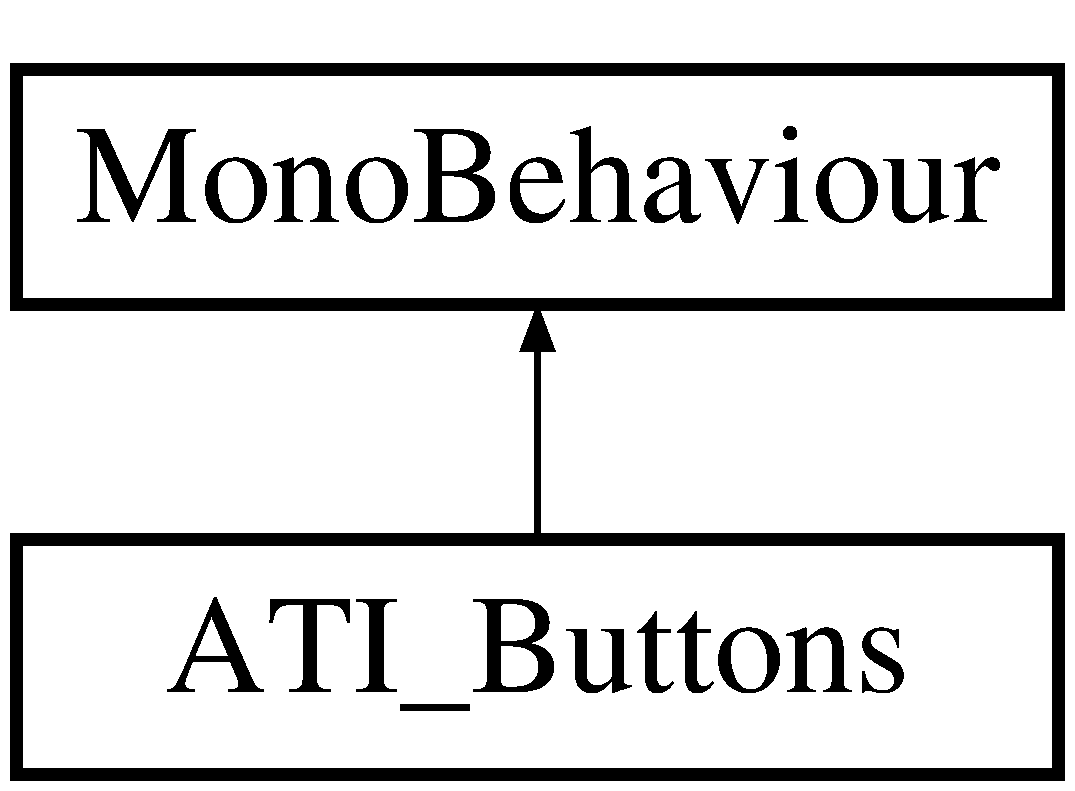
\includegraphics[height=2.000000cm]{class_a_t_i___buttons}
\end{center}
\end{figure}
\subsection*{Private Member Functions}
\begin{DoxyCompactItemize}
\item 
void \hyperlink{group___a_t_i_buttons_unity_gaa24ae34a40539dab6595d1713fc77560}{Awake} ()
\begin{DoxyCompactList}\small\item\em Gets references to the buttons and adds their listeners. Called when the object is created. \end{DoxyCompactList}\item 
void \hyperlink{group___a_t_i_buttons_unity_ga1b9e9b75184e9e26309cc14bda37ad8a}{On\+Load\+Keyboard\+Scene\+Button\+Clicked} ()
\begin{DoxyCompactList}\small\item\em Loads the song creation interface scene. \end{DoxyCompactList}\item 
void \hyperlink{group___a_t_i_buttons_unity_ga6f6e66c53a80c3bcd9b7e7238a3b82fd}{On\+Load\+Song\+Creation\+Button\+Clicked} ()
\begin{DoxyCompactList}\small\item\em Loads the song creation interface scene. \end{DoxyCompactList}\end{DoxyCompactItemize}
\subsection*{Private Attributes}
\begin{DoxyCompactItemize}
\item 
Button \hyperlink{group___a_t_i_buttons_priv_var_ga8ab732143834bd94387cfd94c59886da}{m\+Load\+Song\+Creation\+Button} = null
\begin{DoxyCompactList}\small\item\em The button that loads the song creation interface when clicked. \end{DoxyCompactList}\item 
Button \hyperlink{group___a_t_i_buttons_priv_var_ga7b2f643a87f99b6a35a2d64330c8a9d4}{m\+Load\+Keyboard\+Scene\+Button} = null
\begin{DoxyCompactList}\small\item\em The button that loads the keyboard scene. \end{DoxyCompactList}\end{DoxyCompactItemize}


\subsection{Detailed Description}
Handler for buttons on the Audio Testing Interface. 

Definition at line 12 of file A\+T\+I\+\_\+\+Buttons.\+cs.



The documentation for this class was generated from the following file\+:\begin{DoxyCompactItemize}
\item 
D\+:/\+Documents/\+School Documents/2017\+Spring/\+E\+E\+C\+S542/\+V\+R\+Piano\+Project/\+Assets/\+Scripts/\+Audio/\+Testing/\hyperlink{_a_t_i___buttons_8cs}{A\+T\+I\+\_\+\+Buttons.\+cs}\end{DoxyCompactItemize}

\hypertarget{class_a_t_i___demo_song_button_handler}{}\section{A\+T\+I\+\_\+\+Demo\+Song\+Button\+Handler Class Reference}
\label{class_a_t_i___demo_song_button_handler}\index{A\+T\+I\+\_\+\+Demo\+Song\+Button\+Handler@{A\+T\+I\+\_\+\+Demo\+Song\+Button\+Handler}}
Inheritance diagram for A\+T\+I\+\_\+\+Demo\+Song\+Button\+Handler\+:\begin{figure}[H]
\begin{center}
\leavevmode
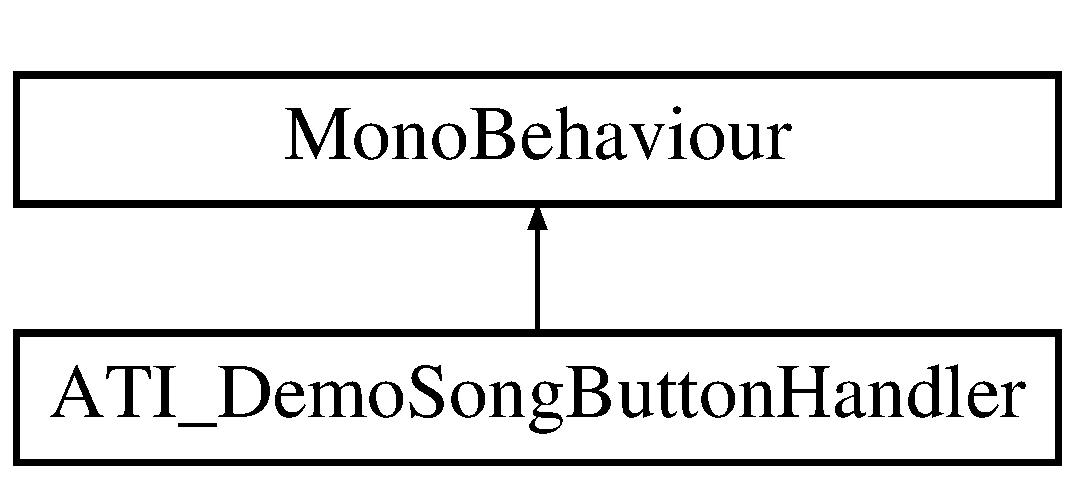
\includegraphics[height=2.000000cm]{class_a_t_i___demo_song_button_handler}
\end{center}
\end{figure}
\subsection*{Public Member Functions}
\begin{DoxyCompactItemize}
\item 
void \hyperlink{class_a_t_i___demo_song_button_handler_a584b9dd672e492fe0df592061c7733de}{Load\+Demo\+Song} (int a\+Index)
\item 
void \hyperlink{class_a_t_i___demo_song_button_handler_a9a7fc268b3021a826dc4ad031a856dfc}{Change\+B\+PM} (float a\+B\+PM)
\item 
void \hyperlink{class_a_t_i___demo_song_button_handler_a2801913e33a297ae1f5db91f851ddea6}{Handle\+Instrument\+Change} (\hyperlink{group___music_enums_gabfce60192305965558a36e368ebd67c3}{Music.\+I\+N\+S\+T\+R\+U\+M\+E\+N\+T\+\_\+\+T\+Y\+PE} a\+Type)
\item 
void \hyperlink{class_a_t_i___demo_song_button_handler_a2b25debcc12ccdd2db23d4339d80f260}{On\+Play\+Pause\+Button\+Clicked} ()
\item 
void \hyperlink{class_a_t_i___demo_song_button_handler_a74b93fb6f260529a0f7260238226677b}{On\+Stop\+Button\+Clicked} ()
\item 
void \hyperlink{class_a_t_i___demo_song_button_handler_aec5406e1eb0c885f0e6fe044cfe4113e}{Set\+Finished} ()
\end{DoxyCompactItemize}
\subsection*{Public Attributes}
\begin{DoxyCompactItemize}
\item 
bool \hyperlink{class_a_t_i___demo_song_button_handler_a772b617c22a316a99f3a4b6979d0657a}{Drum\+Loop\+Selector} = false
\end{DoxyCompactItemize}
\subsection*{Private Member Functions}
\begin{DoxyCompactItemize}
\item 
void \hyperlink{class_a_t_i___demo_song_button_handler_a723e9581adb3cbc7198af345b8c88b66}{Start} ()
\item 
void \hyperlink{class_a_t_i___demo_song_button_handler_a27b2b6ae2ef7d38ba4212bc4ad280247}{Update} ()
\end{DoxyCompactItemize}
\subsection*{Private Attributes}
\begin{DoxyCompactItemize}
\item 
bool \hyperlink{class_a_t_i___demo_song_button_handler_a14e70250c780214dc71d2aae6d638a25}{m\+Active} = true
\item 
bool \hyperlink{class_a_t_i___demo_song_button_handler_a4a9d01d8ee385c66a6a27da6d9d94f18}{m\+Finished} = false
\begin{DoxyCompactList}\small\item\em Is the song finished? \end{DoxyCompactList}\item 
bool \hyperlink{class_a_t_i___demo_song_button_handler_abee877053d95bfba813d61d5a5d87a23}{m\+Paused} = false
\begin{DoxyCompactList}\small\item\em Is the song paused? \end{DoxyCompactList}\item 
bool \hyperlink{class_a_t_i___demo_song_button_handler_aefbba0db111a0d4ba1b1d9f5c1cae41d}{m\+Playing} = false
\begin{DoxyCompactList}\small\item\em Is the song playing? \end{DoxyCompactList}\item 
Button \hyperlink{class_a_t_i___demo_song_button_handler_a9f3be8593e24316510ca461f105061fd}{m\+Play\+Pause\+Button} = null
\item 
Button \hyperlink{class_a_t_i___demo_song_button_handler_ad6a342b9b2333c8c613b968a0ca7545c}{m\+Stop\+Button} = null
\begin{DoxyCompactList}\small\item\em The button to stop the song. \end{DoxyCompactList}\item 
Dropdown \hyperlink{class_a_t_i___demo_song_button_handler_af58c5b6dd392fbf606b74188b02044ce}{m\+Song\+Selection\+Menu} = null
\item 
Slider \hyperlink{class_a_t_i___demo_song_button_handler_a7d1ed48ed81d7fc9fbde52f8ee87600e}{m\+B\+P\+M\+Slider} = null
\item 
\hyperlink{class_song}{Song} \hyperlink{class_a_t_i___demo_song_button_handler_aef782d481c6250a9062162c71298ed8f}{m\+Song} = null
\item 
Sprite \mbox{[}$\,$\mbox{]} \hyperlink{class_a_t_i___demo_song_button_handler_a9d62cca93ee54ba52e0c7de5f30d9490}{m\+Button\+Images} = null
\begin{DoxyCompactList}\small\item\em The images for the buttons. \end{DoxyCompactList}\item 
Text \hyperlink{class_a_t_i___demo_song_button_handler_af884aa63036769a78f92d86084156263}{m\+B\+P\+M\+Slider\+Text} = null
\item 
\hyperlink{class_virtual_instrument_manager}{Virtual\+Instrument\+Manager} \hyperlink{class_a_t_i___demo_song_button_handler_ac078f283ce74a7b310ebb2cbbc55f70b}{m\+V\+IM} = null
\end{DoxyCompactItemize}


\subsection{Detailed Description}


Definition at line 16 of file A\+T\+I\+\_\+\+Demo\+Song\+Button\+Handler.\+cs.



\subsection{Member Function Documentation}
\mbox{\Hypertarget{class_a_t_i___demo_song_button_handler_a9a7fc268b3021a826dc4ad031a856dfc}\label{class_a_t_i___demo_song_button_handler_a9a7fc268b3021a826dc4ad031a856dfc}} 
\index{A\+T\+I\+\_\+\+Demo\+Song\+Button\+Handler@{A\+T\+I\+\_\+\+Demo\+Song\+Button\+Handler}!Change\+B\+PM@{Change\+B\+PM}}
\index{Change\+B\+PM@{Change\+B\+PM}!A\+T\+I\+\_\+\+Demo\+Song\+Button\+Handler@{A\+T\+I\+\_\+\+Demo\+Song\+Button\+Handler}}
\subsubsection{\texorpdfstring{Change\+B\+P\+M()}{ChangeBPM()}}
{\footnotesize\ttfamily void A\+T\+I\+\_\+\+Demo\+Song\+Button\+Handler.\+Change\+B\+PM (\begin{DoxyParamCaption}\item[{float}]{a\+B\+PM }\end{DoxyParamCaption})}



Definition at line 132 of file A\+T\+I\+\_\+\+Demo\+Song\+Button\+Handler.\+cs.



References Song.\+Set\+B\+P\+M().



Referenced by Start().


\begin{DoxyCode}
133     \{
134         \textcolor{comment}{// Update the BPM slider's label.}
135         \hyperlink{class_a_t_i___demo_song_button_handler_af884aa63036769a78f92d86084156263}{mBPMSliderText}.text = \textcolor{stringliteral}{"BPM: "} + aBPM.ToString();
136 
137         \textcolor{comment}{// Update the loaded song.}
138         \hyperlink{class_a_t_i___demo_song_button_handler_aef782d481c6250a9062162c71298ed8f}{mSong}.\hyperlink{group___song_pub_func_gaa65bbba1af7192edff7e0f848029013b}{SetBPM}( aBPM );
139     \}
\end{DoxyCode}
\mbox{\Hypertarget{class_a_t_i___demo_song_button_handler_a2801913e33a297ae1f5db91f851ddea6}\label{class_a_t_i___demo_song_button_handler_a2801913e33a297ae1f5db91f851ddea6}} 
\index{A\+T\+I\+\_\+\+Demo\+Song\+Button\+Handler@{A\+T\+I\+\_\+\+Demo\+Song\+Button\+Handler}!Handle\+Instrument\+Change@{Handle\+Instrument\+Change}}
\index{Handle\+Instrument\+Change@{Handle\+Instrument\+Change}!A\+T\+I\+\_\+\+Demo\+Song\+Button\+Handler@{A\+T\+I\+\_\+\+Demo\+Song\+Button\+Handler}}
\subsubsection{\texorpdfstring{Handle\+Instrument\+Change()}{HandleInstrumentChange()}}
{\footnotesize\ttfamily void A\+T\+I\+\_\+\+Demo\+Song\+Button\+Handler.\+Handle\+Instrument\+Change (\begin{DoxyParamCaption}\item[{\hyperlink{group___music_enums_gabfce60192305965558a36e368ebd67c3}{Music.\+I\+N\+S\+T\+R\+U\+M\+E\+N\+T\+\_\+\+T\+Y\+PE}}]{a\+Type }\end{DoxyParamCaption})}



Definition at line 142 of file A\+T\+I\+\_\+\+Demo\+Song\+Button\+Handler.\+cs.



Referenced by Start().


\begin{DoxyCode}
143     \{
144         \textcolor{keywordflow}{if}( aType == \hyperlink{class_music}{Music}.\hyperlink{group___music_enums_gabfce60192305965558a36e368ebd67c3}{INSTRUMENT\_TYPE}.DRUM\_KIT && !
      \hyperlink{class_a_t_i___demo_song_button_handler_a772b617c22a316a99f3a4b6979d0657a}{DrumLoopSelector} )
145         \{
146             \hyperlink{class_a_t_i___demo_song_button_handler_a14e70250c780214dc71d2aae6d638a25}{mActive} = \textcolor{keyword}{false};
147             \hyperlink{class_a_t_i___demo_song_button_handler_a7d1ed48ed81d7fc9fbde52f8ee87600e}{mBPMSlider}.gameObject.SetActive( \textcolor{keyword}{false} );
148             \hyperlink{class_a_t_i___demo_song_button_handler_a9f3be8593e24316510ca461f105061fd}{mPlayPauseButton}.transform.parent.gameObject.SetActive( \textcolor{keyword}{false} );
149             \hyperlink{class_a_t_i___demo_song_button_handler_ad6a342b9b2333c8c613b968a0ca7545c}{mStopButton}.transform.parent.gameObject.SetActive( \textcolor{keyword}{false} );
150             \hyperlink{class_a_t_i___demo_song_button_handler_af58c5b6dd392fbf606b74188b02044ce}{mSongSelectionMenu}.gameObject.SetActive( \textcolor{keyword}{false} );
151         \}
152         \textcolor{keywordflow}{else} \textcolor{keywordflow}{if}( !\hyperlink{class_a_t_i___demo_song_button_handler_a14e70250c780214dc71d2aae6d638a25}{mActive} )
153         \{
154             \hyperlink{class_a_t_i___demo_song_button_handler_a14e70250c780214dc71d2aae6d638a25}{mActive} = \textcolor{keyword}{true};
155             \hyperlink{class_a_t_i___demo_song_button_handler_a7d1ed48ed81d7fc9fbde52f8ee87600e}{mBPMSlider}.gameObject.SetActive( \textcolor{keyword}{true} );
156             \hyperlink{class_a_t_i___demo_song_button_handler_a9f3be8593e24316510ca461f105061fd}{mPlayPauseButton}.transform.parent.gameObject.SetActive( \textcolor{keyword}{true} );
157             \hyperlink{class_a_t_i___demo_song_button_handler_af58c5b6dd392fbf606b74188b02044ce}{mSongSelectionMenu}.gameObject.SetActive( \textcolor{keyword}{true} );
158         \}
159     \}
\end{DoxyCode}
\mbox{\Hypertarget{class_a_t_i___demo_song_button_handler_a584b9dd672e492fe0df592061c7733de}\label{class_a_t_i___demo_song_button_handler_a584b9dd672e492fe0df592061c7733de}} 
\index{A\+T\+I\+\_\+\+Demo\+Song\+Button\+Handler@{A\+T\+I\+\_\+\+Demo\+Song\+Button\+Handler}!Load\+Demo\+Song@{Load\+Demo\+Song}}
\index{Load\+Demo\+Song@{Load\+Demo\+Song}!A\+T\+I\+\_\+\+Demo\+Song\+Button\+Handler@{A\+T\+I\+\_\+\+Demo\+Song\+Button\+Handler}}
\subsubsection{\texorpdfstring{Load\+Demo\+Song()}{LoadDemoSong()}}
{\footnotesize\ttfamily void A\+T\+I\+\_\+\+Demo\+Song\+Button\+Handler.\+Load\+Demo\+Song (\begin{DoxyParamCaption}\item[{int}]{a\+Index }\end{DoxyParamCaption})}



Definition at line 120 of file A\+T\+I\+\_\+\+Demo\+Song\+Button\+Handler.\+cs.



References Song.\+Get\+B\+P\+M(), Song\+Manager\+Class.\+Get\+Song\+By\+Name(), and Virtual\+Instrument\+Manager.\+Song\+Manager.



Referenced by Start().


\begin{DoxyCode}
121     \{
122         \hyperlink{class_a_t_i___demo_song_button_handler_aef782d481c6250a9062162c71298ed8f}{mSong} = null;
123         \hyperlink{class_a_t_i___demo_song_button_handler_aef782d481c6250a9062162c71298ed8f}{mSong} = \hyperlink{class_a_t_i___demo_song_button_handler_ac078f283ce74a7b310ebb2cbbc55f70b}{mVIM}.\hyperlink{group___v_i_m_pub_ga33dae94932c10c66db76a0eebec76b01}{SongManager}.\hyperlink{group___s_m_pub_func_gafe818c55bd858c52c95a2fa7a566006a}{GetSongByName}( 
      \hyperlink{class_a_t_i___demo_song_button_handler_af58c5b6dd392fbf606b74188b02044ce}{mSongSelectionMenu}.options[aIndex].text );
124         \hyperlink{class_a_t_i___demo_song_button_handler_a7d1ed48ed81d7fc9fbde52f8ee87600e}{mBPMSlider}.value = \hyperlink{class_a_t_i___demo_song_button_handler_aef782d481c6250a9062162c71298ed8f}{mSong}.\hyperlink{group___song_pub_func_gaaaf3d27d474713d7d368e3fd4c570be0}{GetBPM}();
125     \}
\end{DoxyCode}
\mbox{\Hypertarget{class_a_t_i___demo_song_button_handler_a2b25debcc12ccdd2db23d4339d80f260}\label{class_a_t_i___demo_song_button_handler_a2b25debcc12ccdd2db23d4339d80f260}} 
\index{A\+T\+I\+\_\+\+Demo\+Song\+Button\+Handler@{A\+T\+I\+\_\+\+Demo\+Song\+Button\+Handler}!On\+Play\+Pause\+Button\+Clicked@{On\+Play\+Pause\+Button\+Clicked}}
\index{On\+Play\+Pause\+Button\+Clicked@{On\+Play\+Pause\+Button\+Clicked}!A\+T\+I\+\_\+\+Demo\+Song\+Button\+Handler@{A\+T\+I\+\_\+\+Demo\+Song\+Button\+Handler}}
\subsubsection{\texorpdfstring{On\+Play\+Pause\+Button\+Clicked()}{OnPlayPauseButtonClicked()}}
{\footnotesize\ttfamily void A\+T\+I\+\_\+\+Demo\+Song\+Button\+Handler.\+On\+Play\+Pause\+Button\+Clicked (\begin{DoxyParamCaption}{ }\end{DoxyParamCaption})}



Definition at line 162 of file A\+T\+I\+\_\+\+Demo\+Song\+Button\+Handler.\+cs.



References Virtual\+Instrument\+Manager.\+Pause\+Drum\+Loop, Virtual\+Instrument\+Manager.\+Pause\+Song, Virtual\+Instrument\+Manager.\+Play\+Drum\+Loop, Virtual\+Instrument\+Manager.\+Play\+Song, Virtual\+Instrument\+Manager.\+Resume\+Drum\+Loop, and Virtual\+Instrument\+Manager.\+Resume\+Song.



Referenced by Start().


\begin{DoxyCode}
163     \{
164         \textcolor{keywordflow}{if}( \hyperlink{class_a_t_i___demo_song_button_handler_a772b617c22a316a99f3a4b6979d0657a}{DrumLoopSelector} )
165         \{
166             \textcolor{keywordflow}{if}( \hyperlink{class_a_t_i___demo_song_button_handler_aefbba0db111a0d4ba1b1d9f5c1cae41d}{mPlaying} && !\hyperlink{class_a_t_i___demo_song_button_handler_abee877053d95bfba813d61d5a5d87a23}{mPaused} )
167             \{
168                 \hyperlink{class_a_t_i___demo_song_button_handler_ac078f283ce74a7b310ebb2cbbc55f70b}{mVIM}.\hyperlink{group___v_i_m_events_ga6de00a430321852cc3c8c4a213d62c70}{PauseDrumLoop}.Invoke();
169                 \hyperlink{class_a_t_i___demo_song_button_handler_a9f3be8593e24316510ca461f105061fd}{mPlayPauseButton}.image.sprite = \hyperlink{class_a_t_i___demo_song_button_handler_a9d62cca93ee54ba52e0c7de5f30d9490}{mButtonImages}[0];
170                 \hyperlink{class_a_t_i___demo_song_button_handler_abee877053d95bfba813d61d5a5d87a23}{mPaused} = \textcolor{keyword}{true};
171             \}
172             \textcolor{keywordflow}{else} \textcolor{keywordflow}{if}( \hyperlink{class_a_t_i___demo_song_button_handler_abee877053d95bfba813d61d5a5d87a23}{mPaused} )
173             \{
174                 \hyperlink{class_a_t_i___demo_song_button_handler_ac078f283ce74a7b310ebb2cbbc55f70b}{mVIM}.\hyperlink{group___v_i_m_events_ga54db2dc24076cd3cd130e95c2fd5bea0}{ResumeDrumLoop}.Invoke();
175                 \hyperlink{class_a_t_i___demo_song_button_handler_a9f3be8593e24316510ca461f105061fd}{mPlayPauseButton}.image.sprite = \hyperlink{class_a_t_i___demo_song_button_handler_a9d62cca93ee54ba52e0c7de5f30d9490}{mButtonImages}[1];
176                 \hyperlink{class_a_t_i___demo_song_button_handler_abee877053d95bfba813d61d5a5d87a23}{mPaused} = \textcolor{keyword}{false};
177                 \hyperlink{class_a_t_i___demo_song_button_handler_aefbba0db111a0d4ba1b1d9f5c1cae41d}{mPlaying} = \textcolor{keyword}{true};
178             \}
179             \textcolor{keywordflow}{else}
180             \{
181                 \hyperlink{class_a_t_i___demo_song_button_handler_ac078f283ce74a7b310ebb2cbbc55f70b}{mVIM}.\hyperlink{group___v_i_m_events_ga5657ff4bcc7de6d240d7092ffd22a6fe}{PlayDrumLoop}.Invoke( \hyperlink{class_a_t_i___demo_song_button_handler_aef782d481c6250a9062162c71298ed8f}{mSong} );
182                 \hyperlink{class_a_t_i___demo_song_button_handler_ad6a342b9b2333c8c613b968a0ca7545c}{mStopButton}.transform.parent.gameObject.SetActive( \textcolor{keyword}{true} );
183                 \hyperlink{class_a_t_i___demo_song_button_handler_a9f3be8593e24316510ca461f105061fd}{mPlayPauseButton}.image.sprite = \hyperlink{class_a_t_i___demo_song_button_handler_a9d62cca93ee54ba52e0c7de5f30d9490}{mButtonImages}[1];
184                 \hyperlink{class_a_t_i___demo_song_button_handler_aefbba0db111a0d4ba1b1d9f5c1cae41d}{mPlaying} = \textcolor{keyword}{true};
185             \}
186         \}
187         \textcolor{keywordflow}{else}
188         \{
189             \textcolor{keywordflow}{if}( \hyperlink{class_a_t_i___demo_song_button_handler_aefbba0db111a0d4ba1b1d9f5c1cae41d}{mPlaying} && !\hyperlink{class_a_t_i___demo_song_button_handler_abee877053d95bfba813d61d5a5d87a23}{mPaused} )
190             \{
191                 \hyperlink{class_a_t_i___demo_song_button_handler_ac078f283ce74a7b310ebb2cbbc55f70b}{mVIM}.\hyperlink{group___v_i_m_events_gae2d76fc98161d7a4573628dbd93e7887}{PauseSong}.Invoke();
192                 \hyperlink{class_a_t_i___demo_song_button_handler_a9f3be8593e24316510ca461f105061fd}{mPlayPauseButton}.image.sprite = \hyperlink{class_a_t_i___demo_song_button_handler_a9d62cca93ee54ba52e0c7de5f30d9490}{mButtonImages}[0];
193                 \hyperlink{class_a_t_i___demo_song_button_handler_abee877053d95bfba813d61d5a5d87a23}{mPaused} = \textcolor{keyword}{true};
194             \}
195             \textcolor{keywordflow}{else} \textcolor{keywordflow}{if}( \hyperlink{class_a_t_i___demo_song_button_handler_abee877053d95bfba813d61d5a5d87a23}{mPaused} )
196             \{
197                 \hyperlink{class_a_t_i___demo_song_button_handler_ac078f283ce74a7b310ebb2cbbc55f70b}{mVIM}.\hyperlink{group___v_i_m_events_ga01670916ae3917c84a0fb51667f30ab9}{ResumeSong}.Invoke();
198                 \hyperlink{class_a_t_i___demo_song_button_handler_a9f3be8593e24316510ca461f105061fd}{mPlayPauseButton}.image.sprite = \hyperlink{class_a_t_i___demo_song_button_handler_a9d62cca93ee54ba52e0c7de5f30d9490}{mButtonImages}[1];
199                 \hyperlink{class_a_t_i___demo_song_button_handler_abee877053d95bfba813d61d5a5d87a23}{mPaused} = \textcolor{keyword}{false};
200                 \hyperlink{class_a_t_i___demo_song_button_handler_aefbba0db111a0d4ba1b1d9f5c1cae41d}{mPlaying} = \textcolor{keyword}{true};
201             \}
202             \textcolor{keywordflow}{else}
203             \{
204                 \hyperlink{class_a_t_i___demo_song_button_handler_ac078f283ce74a7b310ebb2cbbc55f70b}{mVIM}.\hyperlink{group___v_i_m_events_gae450bdba9c513ab4e43f69def50fa84d}{PlaySong}.Invoke( \hyperlink{class_a_t_i___demo_song_button_handler_aef782d481c6250a9062162c71298ed8f}{mSong} );
205                 \hyperlink{class_a_t_i___demo_song_button_handler_ad6a342b9b2333c8c613b968a0ca7545c}{mStopButton}.transform.parent.gameObject.SetActive( \textcolor{keyword}{true} );
206                 \hyperlink{class_a_t_i___demo_song_button_handler_a9f3be8593e24316510ca461f105061fd}{mPlayPauseButton}.image.sprite = \hyperlink{class_a_t_i___demo_song_button_handler_a9d62cca93ee54ba52e0c7de5f30d9490}{mButtonImages}[1];
207                 \hyperlink{class_a_t_i___demo_song_button_handler_aefbba0db111a0d4ba1b1d9f5c1cae41d}{mPlaying} = \textcolor{keyword}{true};
208             \}
209         \}
210     \}
\end{DoxyCode}
\mbox{\Hypertarget{class_a_t_i___demo_song_button_handler_a74b93fb6f260529a0f7260238226677b}\label{class_a_t_i___demo_song_button_handler_a74b93fb6f260529a0f7260238226677b}} 
\index{A\+T\+I\+\_\+\+Demo\+Song\+Button\+Handler@{A\+T\+I\+\_\+\+Demo\+Song\+Button\+Handler}!On\+Stop\+Button\+Clicked@{On\+Stop\+Button\+Clicked}}
\index{On\+Stop\+Button\+Clicked@{On\+Stop\+Button\+Clicked}!A\+T\+I\+\_\+\+Demo\+Song\+Button\+Handler@{A\+T\+I\+\_\+\+Demo\+Song\+Button\+Handler}}
\subsubsection{\texorpdfstring{On\+Stop\+Button\+Clicked()}{OnStopButtonClicked()}}
{\footnotesize\ttfamily void A\+T\+I\+\_\+\+Demo\+Song\+Button\+Handler.\+On\+Stop\+Button\+Clicked (\begin{DoxyParamCaption}{ }\end{DoxyParamCaption})}



Definition at line 212 of file A\+T\+I\+\_\+\+Demo\+Song\+Button\+Handler.\+cs.



References Virtual\+Instrument\+Manager.\+Stop\+Drum\+Loop, and Virtual\+Instrument\+Manager.\+Stop\+Song.



Referenced by Start().


\begin{DoxyCode}
213     \{
214         Assert.IsTrue( \hyperlink{class_a_t_i___demo_song_button_handler_aefbba0db111a0d4ba1b1d9f5c1cae41d}{mPlaying} || \hyperlink{class_a_t_i___demo_song_button_handler_abee877053d95bfba813d61d5a5d87a23}{mPaused}, \textcolor{stringliteral}{"Somehow we tried to stop a song that wasn't
       playing."} );
215 
216         \hyperlink{class_a_t_i___demo_song_button_handler_ad6a342b9b2333c8c613b968a0ca7545c}{mStopButton}.transform.parent.gameObject.SetActive( \textcolor{keyword}{false} );
217         \hyperlink{class_a_t_i___demo_song_button_handler_aefbba0db111a0d4ba1b1d9f5c1cae41d}{mPlaying} = \textcolor{keyword}{false};
218         \hyperlink{class_a_t_i___demo_song_button_handler_abee877053d95bfba813d61d5a5d87a23}{mPaused} = \textcolor{keyword}{false};
219         \hyperlink{class_a_t_i___demo_song_button_handler_a9f3be8593e24316510ca461f105061fd}{mPlayPauseButton}.image.sprite = \hyperlink{class_a_t_i___demo_song_button_handler_a9d62cca93ee54ba52e0c7de5f30d9490}{mButtonImages}[0];
220 
221         \textcolor{keywordflow}{if}( \hyperlink{class_a_t_i___demo_song_button_handler_a772b617c22a316a99f3a4b6979d0657a}{DrumLoopSelector} )
222         \{
223             \hyperlink{class_a_t_i___demo_song_button_handler_ac078f283ce74a7b310ebb2cbbc55f70b}{mVIM}.\hyperlink{group___v_i_m_events_ga9466995fd3b4a07351a8577042ee8b31}{StopDrumLoop}.Invoke();
224         \}
225         \textcolor{keywordflow}{else}
226         \{
227             \hyperlink{class_a_t_i___demo_song_button_handler_ac078f283ce74a7b310ebb2cbbc55f70b}{mVIM}.\hyperlink{group___v_i_m_events_gaa9e464629814abf2e4db88e240fac72c}{StopSong}.Invoke();
228         \}
229     \}
\end{DoxyCode}
\mbox{\Hypertarget{class_a_t_i___demo_song_button_handler_aec5406e1eb0c885f0e6fe044cfe4113e}\label{class_a_t_i___demo_song_button_handler_aec5406e1eb0c885f0e6fe044cfe4113e}} 
\index{A\+T\+I\+\_\+\+Demo\+Song\+Button\+Handler@{A\+T\+I\+\_\+\+Demo\+Song\+Button\+Handler}!Set\+Finished@{Set\+Finished}}
\index{Set\+Finished@{Set\+Finished}!A\+T\+I\+\_\+\+Demo\+Song\+Button\+Handler@{A\+T\+I\+\_\+\+Demo\+Song\+Button\+Handler}}
\subsubsection{\texorpdfstring{Set\+Finished()}{SetFinished()}}
{\footnotesize\ttfamily void A\+T\+I\+\_\+\+Demo\+Song\+Button\+Handler.\+Set\+Finished (\begin{DoxyParamCaption}{ }\end{DoxyParamCaption})}



Definition at line 231 of file A\+T\+I\+\_\+\+Demo\+Song\+Button\+Handler.\+cs.



Referenced by Start().


\begin{DoxyCode}
232     \{
233         \hyperlink{class_a_t_i___demo_song_button_handler_a4a9d01d8ee385c66a6a27da6d9d94f18}{mFinished} = \textcolor{keyword}{true};
234     \}
\end{DoxyCode}
\mbox{\Hypertarget{class_a_t_i___demo_song_button_handler_a723e9581adb3cbc7198af345b8c88b66}\label{class_a_t_i___demo_song_button_handler_a723e9581adb3cbc7198af345b8c88b66}} 
\index{A\+T\+I\+\_\+\+Demo\+Song\+Button\+Handler@{A\+T\+I\+\_\+\+Demo\+Song\+Button\+Handler}!Start@{Start}}
\index{Start@{Start}!A\+T\+I\+\_\+\+Demo\+Song\+Button\+Handler@{A\+T\+I\+\_\+\+Demo\+Song\+Button\+Handler}}
\subsubsection{\texorpdfstring{Start()}{Start()}}
{\footnotesize\ttfamily void A\+T\+I\+\_\+\+Demo\+Song\+Button\+Handler.\+Start (\begin{DoxyParamCaption}{ }\end{DoxyParamCaption})\hspace{0.3cm}{\ttfamily [private]}}



Definition at line 40 of file A\+T\+I\+\_\+\+Demo\+Song\+Button\+Handler.\+cs.



References Change\+B\+P\+M(), Virtual\+Instrument\+Manager.\+Change\+Instrument, Song.\+Get\+B\+P\+M(), Handle\+Instrument\+Change(), Load\+Demo\+Song(), On\+Play\+Pause\+Button\+Clicked(), On\+Stop\+Button\+Clicked(), and Set\+Finished().


\begin{DoxyCode}
41     \{
42         \textcolor{comment}{// Get the button images.}
43         \hyperlink{class_a_t_i___demo_song_button_handler_a9d62cca93ee54ba52e0c7de5f30d9490}{mButtonImages} = \textcolor{keyword}{new} Sprite[3];
44         \hyperlink{class_a_t_i___demo_song_button_handler_a9d62cca93ee54ba52e0c7de5f30d9490}{mButtonImages}[0] = Resources.Load<Sprite>( \textcolor{stringliteral}{"Audio/Images/play\_button"} );
45         \hyperlink{class_a_t_i___demo_song_button_handler_a9d62cca93ee54ba52e0c7de5f30d9490}{mButtonImages}[1] = Resources.Load<Sprite>( \textcolor{stringliteral}{"Audio/Images/pause\_button"} );
46         mButtonImages[2] = Resources.Load<Sprite>( \textcolor{stringliteral}{"Audio/Images/stop\_button"} );
47 
48         \textcolor{comment}{// Get the virtual instrument manager.}
49         \hyperlink{class_a_t_i___demo_song_button_handler_ac078f283ce74a7b310ebb2cbbc55f70b}{mVIM} = GameObject.Find( \textcolor{stringliteral}{"VirtualInstrumentManager"} ).GetComponent<
      \hyperlink{class_virtual_instrument_manager}{VirtualInstrumentManager}>();
50 
51         \textcolor{comment}{// Account for the VIM changing instruments.}
52         mVIM.\hyperlink{group___v_i_m_events_ga1b9f12a73a5418ea5695d38b78c506c4}{ChangeInstrument}.AddListener( 
      \hyperlink{class_a_t_i___demo_song_button_handler_a2801913e33a297ae1f5db91f851ddea6}{HandleInstrumentChange} );
53 
54         \textcolor{comment}{// Set up the selection menu.}
55         \hyperlink{class_a_t_i___demo_song_button_handler_af58c5b6dd392fbf606b74188b02044ce}{mSongSelectionMenu} = gameObject.GetComponent<Dropdown>();
56         \hyperlink{class_a_t_i___demo_song_button_handler_af58c5b6dd392fbf606b74188b02044ce}{mSongSelectionMenu}.options.Clear();
57 
58         \textcolor{keywordflow}{if}( !\hyperlink{class_a_t_i___demo_song_button_handler_a772b617c22a316a99f3a4b6979d0657a}{DrumLoopSelector} )
59         \{
60             \hyperlink{class_a_t_i___demo_song_button_handler_af58c5b6dd392fbf606b74188b02044ce}{mSongSelectionMenu}.AddOptions( mVIM.SongManager.GetCombinedSongNames() );
61             \hyperlink{class_a_t_i___demo_song_button_handler_af58c5b6dd392fbf606b74188b02044ce}{mSongSelectionMenu}.AddOptions( mVIM.SongManager.GetMelodyNames() );
62             \hyperlink{class_a_t_i___demo_song_button_handler_af58c5b6dd392fbf606b74188b02044ce}{mSongSelectionMenu}.onValueChanged.AddListener( 
      \hyperlink{class_a_t_i___demo_song_button_handler_a584b9dd672e492fe0df592061c7733de}{LoadDemoSong} );
63 
64             \textcolor{comment}{// Load the default demo song.}
65             \hyperlink{class_a_t_i___demo_song_button_handler_aef782d481c6250a9062162c71298ed8f}{mSong} = mVIM.SongManager.GetCombinedSongs()[0];
66         \}
67         \textcolor{keywordflow}{else}
68         \{
69             \hyperlink{class_a_t_i___demo_song_button_handler_af58c5b6dd392fbf606b74188b02044ce}{mSongSelectionMenu}.AddOptions( mVIM.SongManager.GetDrumLoopNames() );
70             \hyperlink{class_a_t_i___demo_song_button_handler_af58c5b6dd392fbf606b74188b02044ce}{mSongSelectionMenu}.onValueChanged.AddListener( 
      \hyperlink{class_a_t_i___demo_song_button_handler_a584b9dd672e492fe0df592061c7733de}{LoadDemoSong} );
71             \hyperlink{class_a_t_i___demo_song_button_handler_aef782d481c6250a9062162c71298ed8f}{mSong} = mVIM.SongManager.GetDrumLoops()[0];
72         \}
73 
74         \textcolor{comment}{// Set up the play button.}
75         \hyperlink{class_a_t_i___demo_song_button_handler_a9f3be8593e24316510ca461f105061fd}{mPlayPauseButton} = gameObject.transform.GetChild( 5 ).GetChild( 0 ).GetComponent<
      Button>();
76         \hyperlink{class_a_t_i___demo_song_button_handler_a9f3be8593e24316510ca461f105061fd}{mPlayPauseButton}.onClick.AddListener( 
      \hyperlink{class_a_t_i___demo_song_button_handler_a2b25debcc12ccdd2db23d4339d80f260}{OnPlayPauseButtonClicked} );
77 
78         \textcolor{comment}{// Set up the stop button}
79         \hyperlink{class_a_t_i___demo_song_button_handler_ad6a342b9b2333c8c613b968a0ca7545c}{mStopButton} = gameObject.transform.GetChild( 6 ).GetChild( 0 ).GetComponent<Button>();
80         \hyperlink{class_a_t_i___demo_song_button_handler_ad6a342b9b2333c8c613b968a0ca7545c}{mStopButton}.onClick.AddListener( \hyperlink{class_a_t_i___demo_song_button_handler_a74b93fb6f260529a0f7260238226677b}{OnStopButtonClicked} );
81         \hyperlink{class_a_t_i___demo_song_button_handler_ad6a342b9b2333c8c613b968a0ca7545c}{mStopButton}.transform.parent.gameObject.SetActive( \textcolor{keyword}{false} );
82 
83         \textcolor{comment}{// Set up the BPM slider.}
84         \hyperlink{class_a_t_i___demo_song_button_handler_a7d1ed48ed81d7fc9fbde52f8ee87600e}{mBPMSlider} = gameObject.transform.GetChild( 4 ).GetComponent<Slider>();
85         \hyperlink{class_a_t_i___demo_song_button_handler_a7d1ed48ed81d7fc9fbde52f8ee87600e}{mBPMSlider}.value = \hyperlink{class_a_t_i___demo_song_button_handler_aef782d481c6250a9062162c71298ed8f}{mSong}.\hyperlink{group___song_pub_func_gaaaf3d27d474713d7d368e3fd4c570be0}{GetBPM}();
86         \hyperlink{class_a_t_i___demo_song_button_handler_a7d1ed48ed81d7fc9fbde52f8ee87600e}{mBPMSlider}.onValueChanged.AddListener( \hyperlink{class_a_t_i___demo_song_button_handler_a9a7fc268b3021a826dc4ad031a856dfc}{ChangeBPM} );
87 
88         \textcolor{comment}{// Set up the BPM slider's label.}
89         \hyperlink{class_a_t_i___demo_song_button_handler_af884aa63036769a78f92d86084156263}{mBPMSliderText} = \hyperlink{class_a_t_i___demo_song_button_handler_a7d1ed48ed81d7fc9fbde52f8ee87600e}{mBPMSlider}.transform.GetChild( 3 ).GetComponent<Text>();
90         \hyperlink{class_a_t_i___demo_song_button_handler_af884aa63036769a78f92d86084156263}{mBPMSliderText}.text = \textcolor{stringliteral}{"BPM: "} + \hyperlink{class_a_t_i___demo_song_button_handler_aef782d481c6250a9062162c71298ed8f}{mSong}.\hyperlink{group___song_pub_func_gaaaf3d27d474713d7d368e3fd4c570be0}{GetBPM}().ToString();
91 
92 
93         
94 
95         \textcolor{comment}{// Add a listener for when the song is finished if needed.}
96         \textcolor{keywordflow}{if}( !\hyperlink{class_a_t_i___demo_song_button_handler_a772b617c22a316a99f3a4b6979d0657a}{DrumLoopSelector} )
97         \{
98             mVIM.AudioFinished.AddListener( \hyperlink{class_a_t_i___demo_song_button_handler_aec5406e1eb0c885f0e6fe044cfe4113e}{SetFinished} );
99         \}
100     \}
\end{DoxyCode}
\mbox{\Hypertarget{class_a_t_i___demo_song_button_handler_a27b2b6ae2ef7d38ba4212bc4ad280247}\label{class_a_t_i___demo_song_button_handler_a27b2b6ae2ef7d38ba4212bc4ad280247}} 
\index{A\+T\+I\+\_\+\+Demo\+Song\+Button\+Handler@{A\+T\+I\+\_\+\+Demo\+Song\+Button\+Handler}!Update@{Update}}
\index{Update@{Update}!A\+T\+I\+\_\+\+Demo\+Song\+Button\+Handler@{A\+T\+I\+\_\+\+Demo\+Song\+Button\+Handler}}
\subsubsection{\texorpdfstring{Update()}{Update()}}
{\footnotesize\ttfamily void A\+T\+I\+\_\+\+Demo\+Song\+Button\+Handler.\+Update (\begin{DoxyParamCaption}{ }\end{DoxyParamCaption})\hspace{0.3cm}{\ttfamily [private]}}



Definition at line 102 of file A\+T\+I\+\_\+\+Demo\+Song\+Button\+Handler.\+cs.


\begin{DoxyCode}
103     \{
104         \textcolor{keywordflow}{if}( \hyperlink{class_a_t_i___demo_song_button_handler_a4a9d01d8ee385c66a6a27da6d9d94f18}{mFinished} )
105         \{
106             \hyperlink{class_a_t_i___demo_song_button_handler_a4a9d01d8ee385c66a6a27da6d9d94f18}{mFinished} = \textcolor{keyword}{false};
107             \hyperlink{class_a_t_i___demo_song_button_handler_ad6a342b9b2333c8c613b968a0ca7545c}{mStopButton}.transform.parent.gameObject.SetActive( \textcolor{keyword}{false} );
108             \hyperlink{class_a_t_i___demo_song_button_handler_aefbba0db111a0d4ba1b1d9f5c1cae41d}{mPlaying} = \textcolor{keyword}{false};
109             \hyperlink{class_a_t_i___demo_song_button_handler_abee877053d95bfba813d61d5a5d87a23}{mPaused} = \textcolor{keyword}{false};
110             \hyperlink{class_a_t_i___demo_song_button_handler_a9f3be8593e24316510ca461f105061fd}{mPlayPauseButton}.image.sprite = \hyperlink{class_a_t_i___demo_song_button_handler_a9d62cca93ee54ba52e0c7de5f30d9490}{mButtonImages}[0];
111 
112         \}
113     \}
\end{DoxyCode}


\subsection{Member Data Documentation}
\mbox{\Hypertarget{class_a_t_i___demo_song_button_handler_a772b617c22a316a99f3a4b6979d0657a}\label{class_a_t_i___demo_song_button_handler_a772b617c22a316a99f3a4b6979d0657a}} 
\index{A\+T\+I\+\_\+\+Demo\+Song\+Button\+Handler@{A\+T\+I\+\_\+\+Demo\+Song\+Button\+Handler}!Drum\+Loop\+Selector@{Drum\+Loop\+Selector}}
\index{Drum\+Loop\+Selector@{Drum\+Loop\+Selector}!A\+T\+I\+\_\+\+Demo\+Song\+Button\+Handler@{A\+T\+I\+\_\+\+Demo\+Song\+Button\+Handler}}
\subsubsection{\texorpdfstring{Drum\+Loop\+Selector}{DrumLoopSelector}}
{\footnotesize\ttfamily bool A\+T\+I\+\_\+\+Demo\+Song\+Button\+Handler.\+Drum\+Loop\+Selector = false}



Definition at line 19 of file A\+T\+I\+\_\+\+Demo\+Song\+Button\+Handler.\+cs.

\mbox{\Hypertarget{class_a_t_i___demo_song_button_handler_a14e70250c780214dc71d2aae6d638a25}\label{class_a_t_i___demo_song_button_handler_a14e70250c780214dc71d2aae6d638a25}} 
\index{A\+T\+I\+\_\+\+Demo\+Song\+Button\+Handler@{A\+T\+I\+\_\+\+Demo\+Song\+Button\+Handler}!m\+Active@{m\+Active}}
\index{m\+Active@{m\+Active}!A\+T\+I\+\_\+\+Demo\+Song\+Button\+Handler@{A\+T\+I\+\_\+\+Demo\+Song\+Button\+Handler}}
\subsubsection{\texorpdfstring{m\+Active}{mActive}}
{\footnotesize\ttfamily bool A\+T\+I\+\_\+\+Demo\+Song\+Button\+Handler.\+m\+Active = true\hspace{0.3cm}{\ttfamily [private]}}



Definition at line 24 of file A\+T\+I\+\_\+\+Demo\+Song\+Button\+Handler.\+cs.

\mbox{\Hypertarget{class_a_t_i___demo_song_button_handler_a7d1ed48ed81d7fc9fbde52f8ee87600e}\label{class_a_t_i___demo_song_button_handler_a7d1ed48ed81d7fc9fbde52f8ee87600e}} 
\index{A\+T\+I\+\_\+\+Demo\+Song\+Button\+Handler@{A\+T\+I\+\_\+\+Demo\+Song\+Button\+Handler}!m\+B\+P\+M\+Slider@{m\+B\+P\+M\+Slider}}
\index{m\+B\+P\+M\+Slider@{m\+B\+P\+M\+Slider}!A\+T\+I\+\_\+\+Demo\+Song\+Button\+Handler@{A\+T\+I\+\_\+\+Demo\+Song\+Button\+Handler}}
\subsubsection{\texorpdfstring{m\+B\+P\+M\+Slider}{mBPMSlider}}
{\footnotesize\ttfamily Slider A\+T\+I\+\_\+\+Demo\+Song\+Button\+Handler.\+m\+B\+P\+M\+Slider = null\hspace{0.3cm}{\ttfamily [private]}}



Definition at line 31 of file A\+T\+I\+\_\+\+Demo\+Song\+Button\+Handler.\+cs.

\mbox{\Hypertarget{class_a_t_i___demo_song_button_handler_af884aa63036769a78f92d86084156263}\label{class_a_t_i___demo_song_button_handler_af884aa63036769a78f92d86084156263}} 
\index{A\+T\+I\+\_\+\+Demo\+Song\+Button\+Handler@{A\+T\+I\+\_\+\+Demo\+Song\+Button\+Handler}!m\+B\+P\+M\+Slider\+Text@{m\+B\+P\+M\+Slider\+Text}}
\index{m\+B\+P\+M\+Slider\+Text@{m\+B\+P\+M\+Slider\+Text}!A\+T\+I\+\_\+\+Demo\+Song\+Button\+Handler@{A\+T\+I\+\_\+\+Demo\+Song\+Button\+Handler}}
\subsubsection{\texorpdfstring{m\+B\+P\+M\+Slider\+Text}{mBPMSliderText}}
{\footnotesize\ttfamily Text A\+T\+I\+\_\+\+Demo\+Song\+Button\+Handler.\+m\+B\+P\+M\+Slider\+Text = null\hspace{0.3cm}{\ttfamily [private]}}



Definition at line 34 of file A\+T\+I\+\_\+\+Demo\+Song\+Button\+Handler.\+cs.

\mbox{\Hypertarget{class_a_t_i___demo_song_button_handler_a9d62cca93ee54ba52e0c7de5f30d9490}\label{class_a_t_i___demo_song_button_handler_a9d62cca93ee54ba52e0c7de5f30d9490}} 
\index{A\+T\+I\+\_\+\+Demo\+Song\+Button\+Handler@{A\+T\+I\+\_\+\+Demo\+Song\+Button\+Handler}!m\+Button\+Images@{m\+Button\+Images}}
\index{m\+Button\+Images@{m\+Button\+Images}!A\+T\+I\+\_\+\+Demo\+Song\+Button\+Handler@{A\+T\+I\+\_\+\+Demo\+Song\+Button\+Handler}}
\subsubsection{\texorpdfstring{m\+Button\+Images}{mButtonImages}}
{\footnotesize\ttfamily Sprite \mbox{[}$\,$\mbox{]} A\+T\+I\+\_\+\+Demo\+Song\+Button\+Handler.\+m\+Button\+Images = null\hspace{0.3cm}{\ttfamily [private]}}



The images for the buttons. 



Definition at line 33 of file A\+T\+I\+\_\+\+Demo\+Song\+Button\+Handler.\+cs.

\mbox{\Hypertarget{class_a_t_i___demo_song_button_handler_a4a9d01d8ee385c66a6a27da6d9d94f18}\label{class_a_t_i___demo_song_button_handler_a4a9d01d8ee385c66a6a27da6d9d94f18}} 
\index{A\+T\+I\+\_\+\+Demo\+Song\+Button\+Handler@{A\+T\+I\+\_\+\+Demo\+Song\+Button\+Handler}!m\+Finished@{m\+Finished}}
\index{m\+Finished@{m\+Finished}!A\+T\+I\+\_\+\+Demo\+Song\+Button\+Handler@{A\+T\+I\+\_\+\+Demo\+Song\+Button\+Handler}}
\subsubsection{\texorpdfstring{m\+Finished}{mFinished}}
{\footnotesize\ttfamily bool A\+T\+I\+\_\+\+Demo\+Song\+Button\+Handler.\+m\+Finished = false\hspace{0.3cm}{\ttfamily [private]}}



Is the song finished? 



Definition at line 25 of file A\+T\+I\+\_\+\+Demo\+Song\+Button\+Handler.\+cs.

\mbox{\Hypertarget{class_a_t_i___demo_song_button_handler_abee877053d95bfba813d61d5a5d87a23}\label{class_a_t_i___demo_song_button_handler_abee877053d95bfba813d61d5a5d87a23}} 
\index{A\+T\+I\+\_\+\+Demo\+Song\+Button\+Handler@{A\+T\+I\+\_\+\+Demo\+Song\+Button\+Handler}!m\+Paused@{m\+Paused}}
\index{m\+Paused@{m\+Paused}!A\+T\+I\+\_\+\+Demo\+Song\+Button\+Handler@{A\+T\+I\+\_\+\+Demo\+Song\+Button\+Handler}}
\subsubsection{\texorpdfstring{m\+Paused}{mPaused}}
{\footnotesize\ttfamily bool A\+T\+I\+\_\+\+Demo\+Song\+Button\+Handler.\+m\+Paused = false\hspace{0.3cm}{\ttfamily [private]}}



Is the song paused? 



Definition at line 26 of file A\+T\+I\+\_\+\+Demo\+Song\+Button\+Handler.\+cs.

\mbox{\Hypertarget{class_a_t_i___demo_song_button_handler_aefbba0db111a0d4ba1b1d9f5c1cae41d}\label{class_a_t_i___demo_song_button_handler_aefbba0db111a0d4ba1b1d9f5c1cae41d}} 
\index{A\+T\+I\+\_\+\+Demo\+Song\+Button\+Handler@{A\+T\+I\+\_\+\+Demo\+Song\+Button\+Handler}!m\+Playing@{m\+Playing}}
\index{m\+Playing@{m\+Playing}!A\+T\+I\+\_\+\+Demo\+Song\+Button\+Handler@{A\+T\+I\+\_\+\+Demo\+Song\+Button\+Handler}}
\subsubsection{\texorpdfstring{m\+Playing}{mPlaying}}
{\footnotesize\ttfamily bool A\+T\+I\+\_\+\+Demo\+Song\+Button\+Handler.\+m\+Playing = false\hspace{0.3cm}{\ttfamily [private]}}



Is the song playing? 



Definition at line 27 of file A\+T\+I\+\_\+\+Demo\+Song\+Button\+Handler.\+cs.

\mbox{\Hypertarget{class_a_t_i___demo_song_button_handler_a9f3be8593e24316510ca461f105061fd}\label{class_a_t_i___demo_song_button_handler_a9f3be8593e24316510ca461f105061fd}} 
\index{A\+T\+I\+\_\+\+Demo\+Song\+Button\+Handler@{A\+T\+I\+\_\+\+Demo\+Song\+Button\+Handler}!m\+Play\+Pause\+Button@{m\+Play\+Pause\+Button}}
\index{m\+Play\+Pause\+Button@{m\+Play\+Pause\+Button}!A\+T\+I\+\_\+\+Demo\+Song\+Button\+Handler@{A\+T\+I\+\_\+\+Demo\+Song\+Button\+Handler}}
\subsubsection{\texorpdfstring{m\+Play\+Pause\+Button}{mPlayPauseButton}}
{\footnotesize\ttfamily Button A\+T\+I\+\_\+\+Demo\+Song\+Button\+Handler.\+m\+Play\+Pause\+Button = null\hspace{0.3cm}{\ttfamily [private]}}



Definition at line 28 of file A\+T\+I\+\_\+\+Demo\+Song\+Button\+Handler.\+cs.

\mbox{\Hypertarget{class_a_t_i___demo_song_button_handler_aef782d481c6250a9062162c71298ed8f}\label{class_a_t_i___demo_song_button_handler_aef782d481c6250a9062162c71298ed8f}} 
\index{A\+T\+I\+\_\+\+Demo\+Song\+Button\+Handler@{A\+T\+I\+\_\+\+Demo\+Song\+Button\+Handler}!m\+Song@{m\+Song}}
\index{m\+Song@{m\+Song}!A\+T\+I\+\_\+\+Demo\+Song\+Button\+Handler@{A\+T\+I\+\_\+\+Demo\+Song\+Button\+Handler}}
\subsubsection{\texorpdfstring{m\+Song}{mSong}}
{\footnotesize\ttfamily \hyperlink{class_song}{Song} A\+T\+I\+\_\+\+Demo\+Song\+Button\+Handler.\+m\+Song = null\hspace{0.3cm}{\ttfamily [private]}}



Definition at line 32 of file A\+T\+I\+\_\+\+Demo\+Song\+Button\+Handler.\+cs.

\mbox{\Hypertarget{class_a_t_i___demo_song_button_handler_af58c5b6dd392fbf606b74188b02044ce}\label{class_a_t_i___demo_song_button_handler_af58c5b6dd392fbf606b74188b02044ce}} 
\index{A\+T\+I\+\_\+\+Demo\+Song\+Button\+Handler@{A\+T\+I\+\_\+\+Demo\+Song\+Button\+Handler}!m\+Song\+Selection\+Menu@{m\+Song\+Selection\+Menu}}
\index{m\+Song\+Selection\+Menu@{m\+Song\+Selection\+Menu}!A\+T\+I\+\_\+\+Demo\+Song\+Button\+Handler@{A\+T\+I\+\_\+\+Demo\+Song\+Button\+Handler}}
\subsubsection{\texorpdfstring{m\+Song\+Selection\+Menu}{mSongSelectionMenu}}
{\footnotesize\ttfamily Dropdown A\+T\+I\+\_\+\+Demo\+Song\+Button\+Handler.\+m\+Song\+Selection\+Menu = null\hspace{0.3cm}{\ttfamily [private]}}



Definition at line 30 of file A\+T\+I\+\_\+\+Demo\+Song\+Button\+Handler.\+cs.

\mbox{\Hypertarget{class_a_t_i___demo_song_button_handler_ad6a342b9b2333c8c613b968a0ca7545c}\label{class_a_t_i___demo_song_button_handler_ad6a342b9b2333c8c613b968a0ca7545c}} 
\index{A\+T\+I\+\_\+\+Demo\+Song\+Button\+Handler@{A\+T\+I\+\_\+\+Demo\+Song\+Button\+Handler}!m\+Stop\+Button@{m\+Stop\+Button}}
\index{m\+Stop\+Button@{m\+Stop\+Button}!A\+T\+I\+\_\+\+Demo\+Song\+Button\+Handler@{A\+T\+I\+\_\+\+Demo\+Song\+Button\+Handler}}
\subsubsection{\texorpdfstring{m\+Stop\+Button}{mStopButton}}
{\footnotesize\ttfamily Button A\+T\+I\+\_\+\+Demo\+Song\+Button\+Handler.\+m\+Stop\+Button = null\hspace{0.3cm}{\ttfamily [private]}}



The button to stop the song. 



Definition at line 29 of file A\+T\+I\+\_\+\+Demo\+Song\+Button\+Handler.\+cs.

\mbox{\Hypertarget{class_a_t_i___demo_song_button_handler_ac078f283ce74a7b310ebb2cbbc55f70b}\label{class_a_t_i___demo_song_button_handler_ac078f283ce74a7b310ebb2cbbc55f70b}} 
\index{A\+T\+I\+\_\+\+Demo\+Song\+Button\+Handler@{A\+T\+I\+\_\+\+Demo\+Song\+Button\+Handler}!m\+V\+IM@{m\+V\+IM}}
\index{m\+V\+IM@{m\+V\+IM}!A\+T\+I\+\_\+\+Demo\+Song\+Button\+Handler@{A\+T\+I\+\_\+\+Demo\+Song\+Button\+Handler}}
\subsubsection{\texorpdfstring{m\+V\+IM}{mVIM}}
{\footnotesize\ttfamily \hyperlink{class_virtual_instrument_manager}{Virtual\+Instrument\+Manager} A\+T\+I\+\_\+\+Demo\+Song\+Button\+Handler.\+m\+V\+IM = null\hspace{0.3cm}{\ttfamily [private]}}



Definition at line 35 of file A\+T\+I\+\_\+\+Demo\+Song\+Button\+Handler.\+cs.



The documentation for this class was generated from the following file\+:\begin{DoxyCompactItemize}
\item 
D\+:/\+Documents/\+School Documents/2017\+Spring/\+E\+E\+C\+S542/\+V\+R\+Piano\+Project/\+Assets/\+Scripts/\+Audio/\+Testing/\hyperlink{_a_t_i___demo_song_button_handler_8cs}{A\+T\+I\+\_\+\+Demo\+Song\+Button\+Handler.\+cs}\end{DoxyCompactItemize}

\hypertarget{class_a_t_i___diagnostics_demo_song_handler}{}\section{A\+T\+I\+\_\+\+Diagnostics\+Demo\+Song\+Handler Class Reference}
\label{class_a_t_i___diagnostics_demo_song_handler}\index{A\+T\+I\+\_\+\+Diagnostics\+Demo\+Song\+Handler@{A\+T\+I\+\_\+\+Diagnostics\+Demo\+Song\+Handler}}
Inheritance diagram for A\+T\+I\+\_\+\+Diagnostics\+Demo\+Song\+Handler\+:\begin{figure}[H]
\begin{center}
\leavevmode
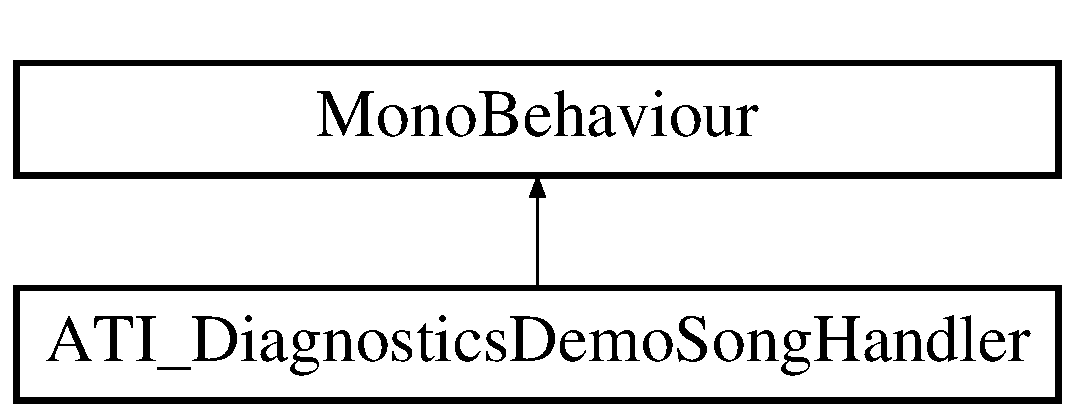
\includegraphics[height=2.000000cm]{class_a_t_i___diagnostics_demo_song_handler}
\end{center}
\end{figure}
\subsection*{Public Member Functions}
\begin{DoxyCompactItemize}
\item 
void \hyperlink{class_a_t_i___diagnostics_demo_song_handler_aecc26edabf9f923007a18c38a6934a5c}{Load\+Demo\+Song} (int a\+Index)
\item 
void \hyperlink{class_a_t_i___diagnostics_demo_song_handler_a860f995ecf2cce11b2a9a3e8fe37237e}{Change\+B\+PM} (float a\+B\+PM)
\item 
void \hyperlink{class_a_t_i___diagnostics_demo_song_handler_acb03659027c98d419fc6ff61dbf24356}{On\+Play\+Button\+Clicked} ()
\end{DoxyCompactItemize}
\subsection*{Private Member Functions}
\begin{DoxyCompactItemize}
\item 
void \hyperlink{class_a_t_i___diagnostics_demo_song_handler_a86f25504d9704a3f330328c476f890c4}{Start} ()
\end{DoxyCompactItemize}
\subsection*{Private Attributes}
\begin{DoxyCompactItemize}
\item 
Button \hyperlink{class_a_t_i___diagnostics_demo_song_handler_a364615af222e630eaca110b6d2afdec5}{m\+Play\+Button} = null
\item 
Dropdown \hyperlink{class_a_t_i___diagnostics_demo_song_handler_a9c44359a719997d03d3ce26afa5609db}{m\+Song\+Selection\+Menu} = null
\item 
Slider \hyperlink{class_a_t_i___diagnostics_demo_song_handler_ad501644f4b61fe763b75e5b63aa5badc}{m\+B\+P\+M\+Slider} = null
\item 
\hyperlink{class_song}{Song} \hyperlink{class_a_t_i___diagnostics_demo_song_handler_a8d34a075cf131a43db5e81cba4c9ea9d}{m\+Song} = null
\item 
Sprite \mbox{[}$\,$\mbox{]} \hyperlink{class_a_t_i___diagnostics_demo_song_handler_a26af0da356a95b5be50bb84647674c84}{m\+Button\+Images} = null
\begin{DoxyCompactList}\small\item\em The images for the buttons. \end{DoxyCompactList}\item 
Text \hyperlink{class_a_t_i___diagnostics_demo_song_handler_ada25fecbd1bc9aaf468b3206d62a9193}{m\+B\+P\+M\+Slider\+Text} = null
\item 
\hyperlink{class_virtual_instrument_manager}{Virtual\+Instrument\+Manager} \hyperlink{class_a_t_i___diagnostics_demo_song_handler_ac3a2216a6de2023d3dd19caa25de7d6f}{m\+V\+IM} = null
\end{DoxyCompactItemize}


\subsection{Detailed Description}


Definition at line 16 of file A\+T\+I\+\_\+\+Diagnostics\+Demo\+Song\+Handler.\+cs.



\subsection{Member Function Documentation}
\mbox{\Hypertarget{class_a_t_i___diagnostics_demo_song_handler_a860f995ecf2cce11b2a9a3e8fe37237e}\label{class_a_t_i___diagnostics_demo_song_handler_a860f995ecf2cce11b2a9a3e8fe37237e}} 
\index{A\+T\+I\+\_\+\+Diagnostics\+Demo\+Song\+Handler@{A\+T\+I\+\_\+\+Diagnostics\+Demo\+Song\+Handler}!Change\+B\+PM@{Change\+B\+PM}}
\index{Change\+B\+PM@{Change\+B\+PM}!A\+T\+I\+\_\+\+Diagnostics\+Demo\+Song\+Handler@{A\+T\+I\+\_\+\+Diagnostics\+Demo\+Song\+Handler}}
\subsubsection{\texorpdfstring{Change\+B\+P\+M()}{ChangeBPM()}}
{\footnotesize\ttfamily void A\+T\+I\+\_\+\+Diagnostics\+Demo\+Song\+Handler.\+Change\+B\+PM (\begin{DoxyParamCaption}\item[{float}]{a\+B\+PM }\end{DoxyParamCaption})}



Definition at line 86 of file A\+T\+I\+\_\+\+Diagnostics\+Demo\+Song\+Handler.\+cs.



References Song.\+Set\+B\+P\+M().



Referenced by Start().


\begin{DoxyCode}
87     \{
88         \textcolor{comment}{// Update the BPM slider's label.}
89         \hyperlink{class_a_t_i___diagnostics_demo_song_handler_ada25fecbd1bc9aaf468b3206d62a9193}{mBPMSliderText}.text = \textcolor{stringliteral}{"BPM: "} + aBPM.ToString();
90 
91         \textcolor{comment}{// Update the loaded song.}
92         \hyperlink{class_a_t_i___diagnostics_demo_song_handler_a8d34a075cf131a43db5e81cba4c9ea9d}{mSong}.\hyperlink{group___song_pub_func_gaa65bbba1af7192edff7e0f848029013b}{SetBPM}( aBPM );
93     \}
\end{DoxyCode}
\mbox{\Hypertarget{class_a_t_i___diagnostics_demo_song_handler_aecc26edabf9f923007a18c38a6934a5c}\label{class_a_t_i___diagnostics_demo_song_handler_aecc26edabf9f923007a18c38a6934a5c}} 
\index{A\+T\+I\+\_\+\+Diagnostics\+Demo\+Song\+Handler@{A\+T\+I\+\_\+\+Diagnostics\+Demo\+Song\+Handler}!Load\+Demo\+Song@{Load\+Demo\+Song}}
\index{Load\+Demo\+Song@{Load\+Demo\+Song}!A\+T\+I\+\_\+\+Diagnostics\+Demo\+Song\+Handler@{A\+T\+I\+\_\+\+Diagnostics\+Demo\+Song\+Handler}}
\subsubsection{\texorpdfstring{Load\+Demo\+Song()}{LoadDemoSong()}}
{\footnotesize\ttfamily void A\+T\+I\+\_\+\+Diagnostics\+Demo\+Song\+Handler.\+Load\+Demo\+Song (\begin{DoxyParamCaption}\item[{int}]{a\+Index }\end{DoxyParamCaption})}



Definition at line 74 of file A\+T\+I\+\_\+\+Diagnostics\+Demo\+Song\+Handler.\+cs.



References Song.\+Get\+B\+P\+M(), Song\+Manager\+Class.\+Get\+Song\+By\+Name(), and Virtual\+Instrument\+Manager.\+Song\+Manager.



Referenced by Start().


\begin{DoxyCode}
75     \{
76         \hyperlink{class_a_t_i___diagnostics_demo_song_handler_a8d34a075cf131a43db5e81cba4c9ea9d}{mSong} = null;
77         \hyperlink{class_a_t_i___diagnostics_demo_song_handler_a8d34a075cf131a43db5e81cba4c9ea9d}{mSong} = \hyperlink{class_a_t_i___diagnostics_demo_song_handler_ac3a2216a6de2023d3dd19caa25de7d6f}{mVIM}.\hyperlink{group___v_i_m_pub_ga33dae94932c10c66db76a0eebec76b01}{SongManager}.\hyperlink{group___s_m_pub_func_gafe818c55bd858c52c95a2fa7a566006a}{GetSongByName}( 
      \hyperlink{class_a_t_i___diagnostics_demo_song_handler_a9c44359a719997d03d3ce26afa5609db}{mSongSelectionMenu}.options[aIndex].text );
78         \hyperlink{class_a_t_i___diagnostics_demo_song_handler_ad501644f4b61fe763b75e5b63aa5badc}{mBPMSlider}.value = \hyperlink{class_a_t_i___diagnostics_demo_song_handler_a8d34a075cf131a43db5e81cba4c9ea9d}{mSong}.\hyperlink{group___song_pub_func_gaaaf3d27d474713d7d368e3fd4c570be0}{GetBPM}();
79     \}
\end{DoxyCode}
\mbox{\Hypertarget{class_a_t_i___diagnostics_demo_song_handler_acb03659027c98d419fc6ff61dbf24356}\label{class_a_t_i___diagnostics_demo_song_handler_acb03659027c98d419fc6ff61dbf24356}} 
\index{A\+T\+I\+\_\+\+Diagnostics\+Demo\+Song\+Handler@{A\+T\+I\+\_\+\+Diagnostics\+Demo\+Song\+Handler}!On\+Play\+Button\+Clicked@{On\+Play\+Button\+Clicked}}
\index{On\+Play\+Button\+Clicked@{On\+Play\+Button\+Clicked}!A\+T\+I\+\_\+\+Diagnostics\+Demo\+Song\+Handler@{A\+T\+I\+\_\+\+Diagnostics\+Demo\+Song\+Handler}}
\subsubsection{\texorpdfstring{On\+Play\+Button\+Clicked()}{OnPlayButtonClicked()}}
{\footnotesize\ttfamily void A\+T\+I\+\_\+\+Diagnostics\+Demo\+Song\+Handler.\+On\+Play\+Button\+Clicked (\begin{DoxyParamCaption}{ }\end{DoxyParamCaption})}



Definition at line 96 of file A\+T\+I\+\_\+\+Diagnostics\+Demo\+Song\+Handler.\+cs.



References Virtual\+Instrument\+Manager.\+Play\+Song.



Referenced by Start().


\begin{DoxyCode}
97     \{
98         \hyperlink{class_a_t_i___diagnostics_demo_song_handler_ac3a2216a6de2023d3dd19caa25de7d6f}{mVIM}.\hyperlink{group___v_i_m_events_gae450bdba9c513ab4e43f69def50fa84d}{PlaySong}.Invoke( \hyperlink{class_a_t_i___diagnostics_demo_song_handler_a8d34a075cf131a43db5e81cba4c9ea9d}{mSong} );
99     \}
\end{DoxyCode}
\mbox{\Hypertarget{class_a_t_i___diagnostics_demo_song_handler_a86f25504d9704a3f330328c476f890c4}\label{class_a_t_i___diagnostics_demo_song_handler_a86f25504d9704a3f330328c476f890c4}} 
\index{A\+T\+I\+\_\+\+Diagnostics\+Demo\+Song\+Handler@{A\+T\+I\+\_\+\+Diagnostics\+Demo\+Song\+Handler}!Start@{Start}}
\index{Start@{Start}!A\+T\+I\+\_\+\+Diagnostics\+Demo\+Song\+Handler@{A\+T\+I\+\_\+\+Diagnostics\+Demo\+Song\+Handler}}
\subsubsection{\texorpdfstring{Start()}{Start()}}
{\footnotesize\ttfamily void A\+T\+I\+\_\+\+Diagnostics\+Demo\+Song\+Handler.\+Start (\begin{DoxyParamCaption}{ }\end{DoxyParamCaption})\hspace{0.3cm}{\ttfamily [private]}}



Definition at line 32 of file A\+T\+I\+\_\+\+Diagnostics\+Demo\+Song\+Handler.\+cs.



References Change\+B\+P\+M(), Song.\+Get\+B\+P\+M(), Load\+Demo\+Song(), and On\+Play\+Button\+Clicked().


\begin{DoxyCode}
33     \{
34         \textcolor{comment}{// Get the button images.}
35         \hyperlink{class_a_t_i___diagnostics_demo_song_handler_a26af0da356a95b5be50bb84647674c84}{mButtonImages} = \textcolor{keyword}{new} Sprite[3];
36         \hyperlink{class_a_t_i___diagnostics_demo_song_handler_a26af0da356a95b5be50bb84647674c84}{mButtonImages}[0] = Resources.Load<Sprite>( \textcolor{stringliteral}{"Audio/Images/play\_button"} );
37         \hyperlink{class_a_t_i___diagnostics_demo_song_handler_a26af0da356a95b5be50bb84647674c84}{mButtonImages}[1] = Resources.Load<Sprite>( \textcolor{stringliteral}{"Audio/Images/pause\_button"} );
38         mButtonImages[2] = Resources.Load<Sprite>( \textcolor{stringliteral}{"Audio/Images/stop\_button"} );
39 
40         \textcolor{comment}{// Get the virtual instrument manager.}
41         \hyperlink{class_a_t_i___diagnostics_demo_song_handler_ac3a2216a6de2023d3dd19caa25de7d6f}{mVIM} = GameObject.Find( \textcolor{stringliteral}{"VirtualInstrumentManager"} ).GetComponent<
      \hyperlink{class_virtual_instrument_manager}{VirtualInstrumentManager}>();
42 
43         \textcolor{comment}{// Set up the selection menu.}
44         \hyperlink{class_a_t_i___diagnostics_demo_song_handler_a9c44359a719997d03d3ce26afa5609db}{mSongSelectionMenu} = gameObject.GetComponent<Dropdown>();
45         mSongSelectionMenu.options.Clear();
46 
47         mSongSelectionMenu.AddOptions( mVIM.SongManager.GetCombinedSongNames() );
48         mSongSelectionMenu.AddOptions( mVIM.SongManager.GetMelodyNames() );
49         mSongSelectionMenu.onValueChanged.AddListener( \hyperlink{class_a_t_i___diagnostics_demo_song_handler_aecc26edabf9f923007a18c38a6934a5c}{LoadDemoSong} );
50 
51         \textcolor{comment}{// Load the default demo song.}
52         \hyperlink{class_a_t_i___diagnostics_demo_song_handler_a8d34a075cf131a43db5e81cba4c9ea9d}{mSong} = mVIM.SongManager.GetSongs()[0];
53 
54         \textcolor{comment}{// Set up the play button}
55         \hyperlink{class_a_t_i___diagnostics_demo_song_handler_a364615af222e630eaca110b6d2afdec5}{mPlayButton} = transform.GetChild( 5 ).GetComponent<Button>();
56         \hyperlink{class_a_t_i___diagnostics_demo_song_handler_a364615af222e630eaca110b6d2afdec5}{mPlayButton}.onClick.AddListener( \hyperlink{class_a_t_i___diagnostics_demo_song_handler_acb03659027c98d419fc6ff61dbf24356}{OnPlayButtonClicked} );
57 
58         \textcolor{comment}{// Set up the BPM slider.}
59         \hyperlink{class_a_t_i___diagnostics_demo_song_handler_ad501644f4b61fe763b75e5b63aa5badc}{mBPMSlider} = gameObject.transform.GetChild( 4 ).GetComponent<Slider>();
60         \hyperlink{class_a_t_i___diagnostics_demo_song_handler_ad501644f4b61fe763b75e5b63aa5badc}{mBPMSlider}.value = \hyperlink{class_a_t_i___diagnostics_demo_song_handler_a8d34a075cf131a43db5e81cba4c9ea9d}{mSong}.\hyperlink{group___song_pub_func_gaaaf3d27d474713d7d368e3fd4c570be0}{GetBPM}();
61         \hyperlink{class_a_t_i___diagnostics_demo_song_handler_ad501644f4b61fe763b75e5b63aa5badc}{mBPMSlider}.onValueChanged.AddListener( \hyperlink{class_a_t_i___diagnostics_demo_song_handler_a860f995ecf2cce11b2a9a3e8fe37237e}{ChangeBPM} );
62 
63         \textcolor{comment}{// Set up the BPM slider's label.}
64         \hyperlink{class_a_t_i___diagnostics_demo_song_handler_ada25fecbd1bc9aaf468b3206d62a9193}{mBPMSliderText} = \hyperlink{class_a_t_i___diagnostics_demo_song_handler_ad501644f4b61fe763b75e5b63aa5badc}{mBPMSlider}.transform.GetChild( 3 ).GetComponent<Text>();
65         \hyperlink{class_a_t_i___diagnostics_demo_song_handler_ada25fecbd1bc9aaf468b3206d62a9193}{mBPMSliderText}.text = \textcolor{stringliteral}{"BPM: "} + \hyperlink{class_a_t_i___diagnostics_demo_song_handler_a8d34a075cf131a43db5e81cba4c9ea9d}{mSong}.\hyperlink{group___song_pub_func_gaaaf3d27d474713d7d368e3fd4c570be0}{GetBPM}().ToString();
66 
67     \}
\end{DoxyCode}


\subsection{Member Data Documentation}
\mbox{\Hypertarget{class_a_t_i___diagnostics_demo_song_handler_ad501644f4b61fe763b75e5b63aa5badc}\label{class_a_t_i___diagnostics_demo_song_handler_ad501644f4b61fe763b75e5b63aa5badc}} 
\index{A\+T\+I\+\_\+\+Diagnostics\+Demo\+Song\+Handler@{A\+T\+I\+\_\+\+Diagnostics\+Demo\+Song\+Handler}!m\+B\+P\+M\+Slider@{m\+B\+P\+M\+Slider}}
\index{m\+B\+P\+M\+Slider@{m\+B\+P\+M\+Slider}!A\+T\+I\+\_\+\+Diagnostics\+Demo\+Song\+Handler@{A\+T\+I\+\_\+\+Diagnostics\+Demo\+Song\+Handler}}
\subsubsection{\texorpdfstring{m\+B\+P\+M\+Slider}{mBPMSlider}}
{\footnotesize\ttfamily Slider A\+T\+I\+\_\+\+Diagnostics\+Demo\+Song\+Handler.\+m\+B\+P\+M\+Slider = null\hspace{0.3cm}{\ttfamily [private]}}



Definition at line 23 of file A\+T\+I\+\_\+\+Diagnostics\+Demo\+Song\+Handler.\+cs.

\mbox{\Hypertarget{class_a_t_i___diagnostics_demo_song_handler_ada25fecbd1bc9aaf468b3206d62a9193}\label{class_a_t_i___diagnostics_demo_song_handler_ada25fecbd1bc9aaf468b3206d62a9193}} 
\index{A\+T\+I\+\_\+\+Diagnostics\+Demo\+Song\+Handler@{A\+T\+I\+\_\+\+Diagnostics\+Demo\+Song\+Handler}!m\+B\+P\+M\+Slider\+Text@{m\+B\+P\+M\+Slider\+Text}}
\index{m\+B\+P\+M\+Slider\+Text@{m\+B\+P\+M\+Slider\+Text}!A\+T\+I\+\_\+\+Diagnostics\+Demo\+Song\+Handler@{A\+T\+I\+\_\+\+Diagnostics\+Demo\+Song\+Handler}}
\subsubsection{\texorpdfstring{m\+B\+P\+M\+Slider\+Text}{mBPMSliderText}}
{\footnotesize\ttfamily Text A\+T\+I\+\_\+\+Diagnostics\+Demo\+Song\+Handler.\+m\+B\+P\+M\+Slider\+Text = null\hspace{0.3cm}{\ttfamily [private]}}



Definition at line 26 of file A\+T\+I\+\_\+\+Diagnostics\+Demo\+Song\+Handler.\+cs.

\mbox{\Hypertarget{class_a_t_i___diagnostics_demo_song_handler_a26af0da356a95b5be50bb84647674c84}\label{class_a_t_i___diagnostics_demo_song_handler_a26af0da356a95b5be50bb84647674c84}} 
\index{A\+T\+I\+\_\+\+Diagnostics\+Demo\+Song\+Handler@{A\+T\+I\+\_\+\+Diagnostics\+Demo\+Song\+Handler}!m\+Button\+Images@{m\+Button\+Images}}
\index{m\+Button\+Images@{m\+Button\+Images}!A\+T\+I\+\_\+\+Diagnostics\+Demo\+Song\+Handler@{A\+T\+I\+\_\+\+Diagnostics\+Demo\+Song\+Handler}}
\subsubsection{\texorpdfstring{m\+Button\+Images}{mButtonImages}}
{\footnotesize\ttfamily Sprite \mbox{[}$\,$\mbox{]} A\+T\+I\+\_\+\+Diagnostics\+Demo\+Song\+Handler.\+m\+Button\+Images = null\hspace{0.3cm}{\ttfamily [private]}}



The images for the buttons. 



Definition at line 25 of file A\+T\+I\+\_\+\+Diagnostics\+Demo\+Song\+Handler.\+cs.

\mbox{\Hypertarget{class_a_t_i___diagnostics_demo_song_handler_a364615af222e630eaca110b6d2afdec5}\label{class_a_t_i___diagnostics_demo_song_handler_a364615af222e630eaca110b6d2afdec5}} 
\index{A\+T\+I\+\_\+\+Diagnostics\+Demo\+Song\+Handler@{A\+T\+I\+\_\+\+Diagnostics\+Demo\+Song\+Handler}!m\+Play\+Button@{m\+Play\+Button}}
\index{m\+Play\+Button@{m\+Play\+Button}!A\+T\+I\+\_\+\+Diagnostics\+Demo\+Song\+Handler@{A\+T\+I\+\_\+\+Diagnostics\+Demo\+Song\+Handler}}
\subsubsection{\texorpdfstring{m\+Play\+Button}{mPlayButton}}
{\footnotesize\ttfamily Button A\+T\+I\+\_\+\+Diagnostics\+Demo\+Song\+Handler.\+m\+Play\+Button = null\hspace{0.3cm}{\ttfamily [private]}}



Definition at line 21 of file A\+T\+I\+\_\+\+Diagnostics\+Demo\+Song\+Handler.\+cs.

\mbox{\Hypertarget{class_a_t_i___diagnostics_demo_song_handler_a8d34a075cf131a43db5e81cba4c9ea9d}\label{class_a_t_i___diagnostics_demo_song_handler_a8d34a075cf131a43db5e81cba4c9ea9d}} 
\index{A\+T\+I\+\_\+\+Diagnostics\+Demo\+Song\+Handler@{A\+T\+I\+\_\+\+Diagnostics\+Demo\+Song\+Handler}!m\+Song@{m\+Song}}
\index{m\+Song@{m\+Song}!A\+T\+I\+\_\+\+Diagnostics\+Demo\+Song\+Handler@{A\+T\+I\+\_\+\+Diagnostics\+Demo\+Song\+Handler}}
\subsubsection{\texorpdfstring{m\+Song}{mSong}}
{\footnotesize\ttfamily \hyperlink{class_song}{Song} A\+T\+I\+\_\+\+Diagnostics\+Demo\+Song\+Handler.\+m\+Song = null\hspace{0.3cm}{\ttfamily [private]}}



Definition at line 24 of file A\+T\+I\+\_\+\+Diagnostics\+Demo\+Song\+Handler.\+cs.

\mbox{\Hypertarget{class_a_t_i___diagnostics_demo_song_handler_a9c44359a719997d03d3ce26afa5609db}\label{class_a_t_i___diagnostics_demo_song_handler_a9c44359a719997d03d3ce26afa5609db}} 
\index{A\+T\+I\+\_\+\+Diagnostics\+Demo\+Song\+Handler@{A\+T\+I\+\_\+\+Diagnostics\+Demo\+Song\+Handler}!m\+Song\+Selection\+Menu@{m\+Song\+Selection\+Menu}}
\index{m\+Song\+Selection\+Menu@{m\+Song\+Selection\+Menu}!A\+T\+I\+\_\+\+Diagnostics\+Demo\+Song\+Handler@{A\+T\+I\+\_\+\+Diagnostics\+Demo\+Song\+Handler}}
\subsubsection{\texorpdfstring{m\+Song\+Selection\+Menu}{mSongSelectionMenu}}
{\footnotesize\ttfamily Dropdown A\+T\+I\+\_\+\+Diagnostics\+Demo\+Song\+Handler.\+m\+Song\+Selection\+Menu = null\hspace{0.3cm}{\ttfamily [private]}}



Definition at line 22 of file A\+T\+I\+\_\+\+Diagnostics\+Demo\+Song\+Handler.\+cs.

\mbox{\Hypertarget{class_a_t_i___diagnostics_demo_song_handler_ac3a2216a6de2023d3dd19caa25de7d6f}\label{class_a_t_i___diagnostics_demo_song_handler_ac3a2216a6de2023d3dd19caa25de7d6f}} 
\index{A\+T\+I\+\_\+\+Diagnostics\+Demo\+Song\+Handler@{A\+T\+I\+\_\+\+Diagnostics\+Demo\+Song\+Handler}!m\+V\+IM@{m\+V\+IM}}
\index{m\+V\+IM@{m\+V\+IM}!A\+T\+I\+\_\+\+Diagnostics\+Demo\+Song\+Handler@{A\+T\+I\+\_\+\+Diagnostics\+Demo\+Song\+Handler}}
\subsubsection{\texorpdfstring{m\+V\+IM}{mVIM}}
{\footnotesize\ttfamily \hyperlink{class_virtual_instrument_manager}{Virtual\+Instrument\+Manager} A\+T\+I\+\_\+\+Diagnostics\+Demo\+Song\+Handler.\+m\+V\+IM = null\hspace{0.3cm}{\ttfamily [private]}}



Definition at line 27 of file A\+T\+I\+\_\+\+Diagnostics\+Demo\+Song\+Handler.\+cs.



The documentation for this class was generated from the following file\+:\begin{DoxyCompactItemize}
\item 
D\+:/\+Documents/\+School Documents/2017\+Spring/\+E\+E\+C\+S542/\+V\+R\+Piano\+Project/\+Assets/\+Scripts/\+Audio/\+Testing/\hyperlink{_a_t_i___diagnostics_demo_song_handler_8cs}{A\+T\+I\+\_\+\+Diagnostics\+Demo\+Song\+Handler.\+cs}\end{DoxyCompactItemize}

\hypertarget{class_a_t_i___echo_filter_handler}{}\section{A\+T\+I\+\_\+\+Echo\+Filter\+Handler Class Reference}
\label{class_a_t_i___echo_filter_handler}\index{A\+T\+I\+\_\+\+Echo\+Filter\+Handler@{A\+T\+I\+\_\+\+Echo\+Filter\+Handler}}
Inheritance diagram for A\+T\+I\+\_\+\+Echo\+Filter\+Handler\+:\begin{figure}[H]
\begin{center}
\leavevmode
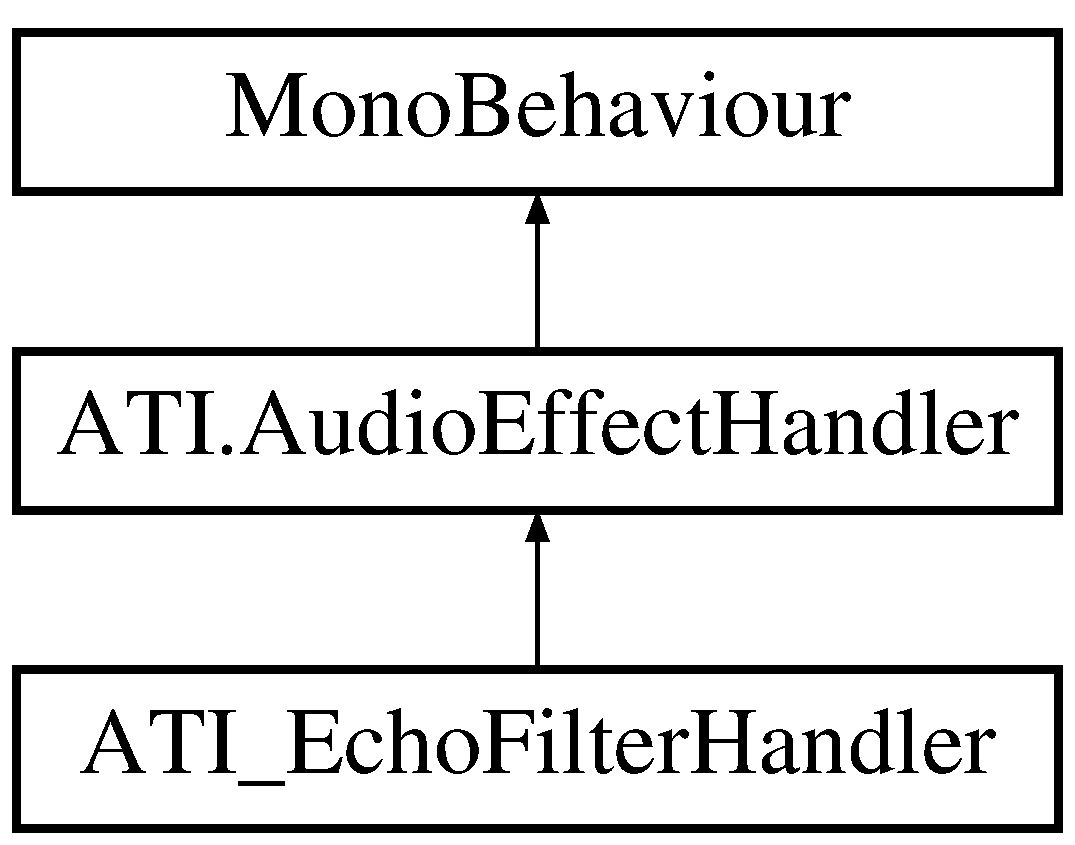
\includegraphics[height=3.000000cm]{class_a_t_i___echo_filter_handler}
\end{center}
\end{figure}
\subsection*{Protected Member Functions}
\begin{DoxyCompactItemize}
\item 
override void \hyperlink{class_a_t_i___echo_filter_handler_a55aed0339fe1f3cdbea2b810a2d74cd4}{Set\+Default\+Parameters} ()
\item 
override void \hyperlink{class_a_t_i___echo_filter_handler_afacef95c6ac470707d2bd092031efac0}{Send\+Parameters\+To\+V\+IM} ()
\item 
override void \hyperlink{class_a_t_i___echo_filter_handler_af759b786ad6e701f816264fefdddb078}{Turn\+On\+Effect} ()
\item 
override void \hyperlink{class_a_t_i___echo_filter_handler_aefc1d2ab19273b9606c09eff2db13165}{Turn\+Off\+Effect} ()
\item 
override void \hyperlink{class_a_t_i___echo_filter_handler_a280746246e42f85d36f96640a7148705}{Handle\+Decay\+Change} (float a\+Value)
\item 
override void \hyperlink{class_a_t_i___echo_filter_handler_a33447b03218ff2945e5f8cea0f8f0d45}{Handle\+Delay\+Change} (float a\+Value)
\item 
override void \hyperlink{class_a_t_i___echo_filter_handler_afc69af9ea7789eb655c01c851594716a}{Handle\+Dry\+Mix\+Change} (float a\+Value)
\item 
override void \hyperlink{class_a_t_i___echo_filter_handler_aef6df1fd85fb153d232191f1bd4de5f3}{Handle\+Scene\+Load} ()
\item 
override void \hyperlink{class_a_t_i___echo_filter_handler_ab64eed11cb12db663a9485bc4bc26fb9}{Handle\+Wet\+Mix\+Change} (float a\+Value)
\end{DoxyCompactItemize}
\subsection*{Private Member Functions}
\begin{DoxyCompactItemize}
\item 
new void \hyperlink{class_a_t_i___echo_filter_handler_a81ac0206d565c1c120dbe9e122474e8e}{Start} ()
\end{DoxyCompactItemize}
\subsection*{Private Attributes}
\begin{DoxyCompactItemize}
\item 
Game\+Object \hyperlink{class_a_t_i___echo_filter_handler_a4e5a10c78852a38c5a6065efdf3f04f8}{m\+Decay\+Container} = null
\item 
Game\+Object \hyperlink{class_a_t_i___echo_filter_handler_a5f454ea9d1603937c5ddb4e3e1f7317d}{m\+Delay\+Container} = null
\item 
Game\+Object \hyperlink{class_a_t_i___echo_filter_handler_a631c4608453cd55ca976926e6e8e8ff2}{m\+Dry\+Mix\+Container} = null
\item 
Game\+Object \hyperlink{class_a_t_i___echo_filter_handler_a571d860b69c4ca4105355d0f1447feb2}{m\+Wet\+Mix\+Container} = null
\item 
\hyperlink{group__filter_params_struct_virtual_instrument_manager_1_1_echo_filter_parameters}{Virtual\+Instrument\+Manager.\+Echo\+Filter\+Parameters} \hyperlink{class_a_t_i___echo_filter_handler_afe435170679cf364951083e6f6ffab36}{m\+Params}
\end{DoxyCompactItemize}
\subsection*{Additional Inherited Members}


\subsection{Detailed Description}


Definition at line 16 of file A\+T\+I\+\_\+\+Echo\+Filter\+Handler.\+cs.



\subsection{Member Function Documentation}
\mbox{\Hypertarget{class_a_t_i___echo_filter_handler_a280746246e42f85d36f96640a7148705}\label{class_a_t_i___echo_filter_handler_a280746246e42f85d36f96640a7148705}} 
\index{A\+T\+I\+\_\+\+Echo\+Filter\+Handler@{A\+T\+I\+\_\+\+Echo\+Filter\+Handler}!Handle\+Decay\+Change@{Handle\+Decay\+Change}}
\index{Handle\+Decay\+Change@{Handle\+Decay\+Change}!A\+T\+I\+\_\+\+Echo\+Filter\+Handler@{A\+T\+I\+\_\+\+Echo\+Filter\+Handler}}
\subsubsection{\texorpdfstring{Handle\+Decay\+Change()}{HandleDecayChange()}}
{\footnotesize\ttfamily override void A\+T\+I\+\_\+\+Echo\+Filter\+Handler.\+Handle\+Decay\+Change (\begin{DoxyParamCaption}\item[{float}]{a\+Value }\end{DoxyParamCaption})\hspace{0.3cm}{\ttfamily [protected]}, {\ttfamily [virtual]}}



Reimplemented from \hyperlink{class_a_t_i_1_1_audio_effect_handler_ae8a88211ac0910dc4b7752667abb2f84}{A\+T\+I.\+Audio\+Effect\+Handler}.



Definition at line 115 of file A\+T\+I\+\_\+\+Echo\+Filter\+Handler.\+cs.



References m\+Params, and Send\+Parameters\+To\+V\+I\+M().


\begin{DoxyCode}
116     \{
117         \hyperlink{class_a_t_i___echo_filter_handler_afe435170679cf364951083e6f6ffab36}{mParams}.Decay = aValue / 100f;
118         \hyperlink{class_a_t_i___echo_filter_handler_afacef95c6ac470707d2bd092031efac0}{SendParametersToVIM}();
119     \}
\end{DoxyCode}
\mbox{\Hypertarget{class_a_t_i___echo_filter_handler_a33447b03218ff2945e5f8cea0f8f0d45}\label{class_a_t_i___echo_filter_handler_a33447b03218ff2945e5f8cea0f8f0d45}} 
\index{A\+T\+I\+\_\+\+Echo\+Filter\+Handler@{A\+T\+I\+\_\+\+Echo\+Filter\+Handler}!Handle\+Delay\+Change@{Handle\+Delay\+Change}}
\index{Handle\+Delay\+Change@{Handle\+Delay\+Change}!A\+T\+I\+\_\+\+Echo\+Filter\+Handler@{A\+T\+I\+\_\+\+Echo\+Filter\+Handler}}
\subsubsection{\texorpdfstring{Handle\+Delay\+Change()}{HandleDelayChange()}}
{\footnotesize\ttfamily override void A\+T\+I\+\_\+\+Echo\+Filter\+Handler.\+Handle\+Delay\+Change (\begin{DoxyParamCaption}\item[{float}]{a\+Value }\end{DoxyParamCaption})\hspace{0.3cm}{\ttfamily [protected]}, {\ttfamily [virtual]}}



Reimplemented from \hyperlink{class_a_t_i_1_1_audio_effect_handler_a5371fca4c2e86cecfc264dfc7559b6bd}{A\+T\+I.\+Audio\+Effect\+Handler}.



Definition at line 123 of file A\+T\+I\+\_\+\+Echo\+Filter\+Handler.\+cs.



References m\+Params, and Send\+Parameters\+To\+V\+I\+M().


\begin{DoxyCode}
124     \{
125         \hyperlink{class_a_t_i___echo_filter_handler_afe435170679cf364951083e6f6ffab36}{mParams}.Delay = aValue;
126         \hyperlink{class_a_t_i___echo_filter_handler_afacef95c6ac470707d2bd092031efac0}{SendParametersToVIM}();
127     \}
\end{DoxyCode}
\mbox{\Hypertarget{class_a_t_i___echo_filter_handler_afc69af9ea7789eb655c01c851594716a}\label{class_a_t_i___echo_filter_handler_afc69af9ea7789eb655c01c851594716a}} 
\index{A\+T\+I\+\_\+\+Echo\+Filter\+Handler@{A\+T\+I\+\_\+\+Echo\+Filter\+Handler}!Handle\+Dry\+Mix\+Change@{Handle\+Dry\+Mix\+Change}}
\index{Handle\+Dry\+Mix\+Change@{Handle\+Dry\+Mix\+Change}!A\+T\+I\+\_\+\+Echo\+Filter\+Handler@{A\+T\+I\+\_\+\+Echo\+Filter\+Handler}}
\subsubsection{\texorpdfstring{Handle\+Dry\+Mix\+Change()}{HandleDryMixChange()}}
{\footnotesize\ttfamily override void A\+T\+I\+\_\+\+Echo\+Filter\+Handler.\+Handle\+Dry\+Mix\+Change (\begin{DoxyParamCaption}\item[{float}]{a\+Value }\end{DoxyParamCaption})\hspace{0.3cm}{\ttfamily [protected]}, {\ttfamily [virtual]}}



Reimplemented from \hyperlink{class_a_t_i_1_1_audio_effect_handler_a8d83371e2e982373b4eb04198a8514fb}{A\+T\+I.\+Audio\+Effect\+Handler}.



Definition at line 131 of file A\+T\+I\+\_\+\+Echo\+Filter\+Handler.\+cs.



References m\+Params, and Send\+Parameters\+To\+V\+I\+M().


\begin{DoxyCode}
132     \{
133         \hyperlink{class_a_t_i___echo_filter_handler_afe435170679cf364951083e6f6ffab36}{mParams}.DryMix = aValue / 100f;
134         \hyperlink{class_a_t_i___echo_filter_handler_afacef95c6ac470707d2bd092031efac0}{SendParametersToVIM}();
135     \}
\end{DoxyCode}
\mbox{\Hypertarget{class_a_t_i___echo_filter_handler_aef6df1fd85fb153d232191f1bd4de5f3}\label{class_a_t_i___echo_filter_handler_aef6df1fd85fb153d232191f1bd4de5f3}} 
\index{A\+T\+I\+\_\+\+Echo\+Filter\+Handler@{A\+T\+I\+\_\+\+Echo\+Filter\+Handler}!Handle\+Scene\+Load@{Handle\+Scene\+Load}}
\index{Handle\+Scene\+Load@{Handle\+Scene\+Load}!A\+T\+I\+\_\+\+Echo\+Filter\+Handler@{A\+T\+I\+\_\+\+Echo\+Filter\+Handler}}
\subsubsection{\texorpdfstring{Handle\+Scene\+Load()}{HandleSceneLoad()}}
{\footnotesize\ttfamily override void A\+T\+I\+\_\+\+Echo\+Filter\+Handler.\+Handle\+Scene\+Load (\begin{DoxyParamCaption}{ }\end{DoxyParamCaption})\hspace{0.3cm}{\ttfamily [protected]}, {\ttfamily [virtual]}}



Reimplemented from \hyperlink{class_a_t_i_1_1_audio_effect_handler_aa038c62089df16a01d2749986649db11}{A\+T\+I.\+Audio\+Effect\+Handler}.



Definition at line 138 of file A\+T\+I\+\_\+\+Echo\+Filter\+Handler.\+cs.



References A\+T\+I.\+Audio\+Effect\+Handler.\+m\+Param\+Object, m\+Params, A\+T\+I.\+Audio\+Effect\+Handler.\+m\+Triggers, A\+T\+I.\+Audio\+Effect\+Parameter\+Trigger.\+Set\+Handler(), A\+T\+I.\+Audio\+Effect\+Parameter\+Trigger.\+Set\+Range(), A\+T\+I.\+Audio\+Effect\+Parameter\+Trigger.\+Set\+Type(), and A\+T\+I.\+Audio\+Effect\+Parameter\+Trigger.\+Set\+Value().


\begin{DoxyCode}
139     \{
140         \textcolor{comment}{// Initialize the AudioEffectParameterTrigger array.}
141         \hyperlink{class_a_t_i_1_1_audio_effect_handler_a1db04dc85daf07d045117d9bc585e944}{mTriggers} = \textcolor{keyword}{new} \hyperlink{class_a_t_i}{ATI}.\hyperlink{class_a_t_i_1_1_audio_effect_parameter_trigger}{AudioEffectParameterTrigger}[4];
142 
143         \textcolor{comment}{// Get the dry mix parameter object and set its values.}
144         \hyperlink{class_a_t_i___echo_filter_handler_a631c4608453cd55ca976926e6e8e8ff2}{mDryMixContainer} = \hyperlink{class_a_t_i_1_1_audio_effect_handler_a02ca13686cb3fc7bf152051ec881b0ed}{mParamObject}.transform.GetChild( 0 ).GetChild( 0 ).
      GetChild( 2 ).gameObject;
145         \hyperlink{class_a_t_i_1_1_audio_effect_handler_a1db04dc85daf07d045117d9bc585e944}{mTriggers}[0] = \hyperlink{class_a_t_i___echo_filter_handler_a631c4608453cd55ca976926e6e8e8ff2}{mDryMixContainer}.AddComponent<
      \hyperlink{class_a_t_i}{ATI}.\hyperlink{class_a_t_i_1_1_audio_effect_parameter_trigger}{AudioEffectParameterTrigger}>();
146         \hyperlink{class_a_t_i_1_1_audio_effect_handler_a1db04dc85daf07d045117d9bc585e944}{mTriggers}[0].\hyperlink{class_a_t_i_1_1_audio_effect_parameter_trigger_a69dc7845ba6454981ce5454ca55b4cb1}{SetHandler}( \textcolor{keyword}{this} );
147         \hyperlink{class_a_t_i_1_1_audio_effect_handler_a1db04dc85daf07d045117d9bc585e944}{mTriggers}[0].\hyperlink{class_a_t_i_1_1_audio_effect_parameter_trigger_a12b9e1d13260a5970f5effed71b9a216}{SetType}( \hyperlink{class_a_t_i}{ATI}.\hyperlink{class_a_t_i_a1123d61b8dceb5867a3683e8d2224ee1}{AudioEffectParameterType}.
      DryMix );
148         \hyperlink{class_a_t_i_1_1_audio_effect_handler_a1db04dc85daf07d045117d9bc585e944}{mTriggers}[0].\hyperlink{class_a_t_i_1_1_audio_effect_parameter_trigger_a3b61498abf2b3e3c8cba23e296ff9273}{SetRange}( 0f, 100f );
149         \hyperlink{class_a_t_i_1_1_audio_effect_handler_a1db04dc85daf07d045117d9bc585e944}{mTriggers}[0].\hyperlink{class_a_t_i_1_1_audio_effect_parameter_trigger_a07ec3a40faeed18c0d85abb035270292}{SetValue}( \hyperlink{class_a_t_i___echo_filter_handler_afe435170679cf364951083e6f6ffab36}{mParams}.DryMix * 100f );
150 
151         \textcolor{comment}{// Get the wet mix parameter object and set its values.}
152         \hyperlink{class_a_t_i___echo_filter_handler_a571d860b69c4ca4105355d0f1447feb2}{mWetMixContainer} = \hyperlink{class_a_t_i_1_1_audio_effect_handler_a02ca13686cb3fc7bf152051ec881b0ed}{mParamObject}.transform.GetChild( 0 ).GetChild( 0 ).
      GetChild( 3 ).gameObject;
153         \hyperlink{class_a_t_i_1_1_audio_effect_handler_a1db04dc85daf07d045117d9bc585e944}{mTriggers}[1] = \hyperlink{class_a_t_i___echo_filter_handler_a571d860b69c4ca4105355d0f1447feb2}{mWetMixContainer}.AddComponent<
      \hyperlink{class_a_t_i}{ATI}.\hyperlink{class_a_t_i_1_1_audio_effect_parameter_trigger}{AudioEffectParameterTrigger}>();
154         \hyperlink{class_a_t_i_1_1_audio_effect_handler_a1db04dc85daf07d045117d9bc585e944}{mTriggers}[1].\hyperlink{class_a_t_i_1_1_audio_effect_parameter_trigger_a69dc7845ba6454981ce5454ca55b4cb1}{SetHandler}( \textcolor{keyword}{this} );
155         \hyperlink{class_a_t_i_1_1_audio_effect_handler_a1db04dc85daf07d045117d9bc585e944}{mTriggers}[1].\hyperlink{class_a_t_i_1_1_audio_effect_parameter_trigger_a12b9e1d13260a5970f5effed71b9a216}{SetType}( \hyperlink{class_a_t_i}{ATI}.\hyperlink{class_a_t_i_a1123d61b8dceb5867a3683e8d2224ee1}{AudioEffectParameterType}.
      WetMix );
156         \hyperlink{class_a_t_i_1_1_audio_effect_handler_a1db04dc85daf07d045117d9bc585e944}{mTriggers}[1].\hyperlink{class_a_t_i_1_1_audio_effect_parameter_trigger_a3b61498abf2b3e3c8cba23e296ff9273}{SetRange}( 0f, 100f );
157         \hyperlink{class_a_t_i_1_1_audio_effect_handler_a1db04dc85daf07d045117d9bc585e944}{mTriggers}[1].\hyperlink{class_a_t_i_1_1_audio_effect_parameter_trigger_a07ec3a40faeed18c0d85abb035270292}{SetValue}( \hyperlink{class_a_t_i___echo_filter_handler_afe435170679cf364951083e6f6ffab36}{mParams}.WetMix * 100f );
158 
159         \textcolor{comment}{// Get the delay parameter object and set its values.}
160         \hyperlink{class_a_t_i___echo_filter_handler_a5f454ea9d1603937c5ddb4e3e1f7317d}{mDelayContainer} = \hyperlink{class_a_t_i_1_1_audio_effect_handler_a02ca13686cb3fc7bf152051ec881b0ed}{mParamObject}.transform.GetChild( 0 ).GetChild( 0 ).
      GetChild( 0 ).gameObject;
161         \hyperlink{class_a_t_i_1_1_audio_effect_handler_a1db04dc85daf07d045117d9bc585e944}{mTriggers}[2] = \hyperlink{class_a_t_i___echo_filter_handler_a5f454ea9d1603937c5ddb4e3e1f7317d}{mDelayContainer}.AddComponent<\hyperlink{class_a_t_i}{ATI}.
      \hyperlink{class_a_t_i_1_1_audio_effect_parameter_trigger}{AudioEffectParameterTrigger}>();
162         \hyperlink{class_a_t_i_1_1_audio_effect_handler_a1db04dc85daf07d045117d9bc585e944}{mTriggers}[2].\hyperlink{class_a_t_i_1_1_audio_effect_parameter_trigger_a69dc7845ba6454981ce5454ca55b4cb1}{SetHandler}( \textcolor{keyword}{this} );
163         \hyperlink{class_a_t_i_1_1_audio_effect_handler_a1db04dc85daf07d045117d9bc585e944}{mTriggers}[2].\hyperlink{class_a_t_i_1_1_audio_effect_parameter_trigger_a12b9e1d13260a5970f5effed71b9a216}{SetType}( \hyperlink{class_a_t_i}{ATI}.\hyperlink{class_a_t_i_a1123d61b8dceb5867a3683e8d2224ee1}{AudioEffectParameterType}.Delay
       );
164         \hyperlink{class_a_t_i_1_1_audio_effect_handler_a1db04dc85daf07d045117d9bc585e944}{mTriggers}[2].\hyperlink{class_a_t_i_1_1_audio_effect_parameter_trigger_a3b61498abf2b3e3c8cba23e296ff9273}{SetRange}( 10f, 5000f );
165         \hyperlink{class_a_t_i_1_1_audio_effect_handler_a1db04dc85daf07d045117d9bc585e944}{mTriggers}[2].\hyperlink{class_a_t_i_1_1_audio_effect_parameter_trigger_a07ec3a40faeed18c0d85abb035270292}{SetValue}( \hyperlink{class_a_t_i___echo_filter_handler_afe435170679cf364951083e6f6ffab36}{mParams}.Delay );
166 
167         \textcolor{comment}{// Get the decay parameter object and set its values.}
168         \hyperlink{class_a_t_i___echo_filter_handler_a4e5a10c78852a38c5a6065efdf3f04f8}{mDecayContainer} = \hyperlink{class_a_t_i_1_1_audio_effect_handler_a02ca13686cb3fc7bf152051ec881b0ed}{mParamObject}.transform.GetChild( 0 ).GetChild( 0 ).
      GetChild( 1 ).gameObject;
169         \hyperlink{class_a_t_i_1_1_audio_effect_handler_a1db04dc85daf07d045117d9bc585e944}{mTriggers}[3] = \hyperlink{class_a_t_i___echo_filter_handler_a4e5a10c78852a38c5a6065efdf3f04f8}{mDecayContainer}.AddComponent<\hyperlink{class_a_t_i}{ATI}.
      \hyperlink{class_a_t_i_1_1_audio_effect_parameter_trigger}{AudioEffectParameterTrigger}>();
170         \hyperlink{class_a_t_i_1_1_audio_effect_handler_a1db04dc85daf07d045117d9bc585e944}{mTriggers}[3].\hyperlink{class_a_t_i_1_1_audio_effect_parameter_trigger_a69dc7845ba6454981ce5454ca55b4cb1}{SetHandler}( \textcolor{keyword}{this} );
171         \hyperlink{class_a_t_i_1_1_audio_effect_handler_a1db04dc85daf07d045117d9bc585e944}{mTriggers}[3].\hyperlink{class_a_t_i_1_1_audio_effect_parameter_trigger_a12b9e1d13260a5970f5effed71b9a216}{SetType}( \hyperlink{class_a_t_i}{ATI}.\hyperlink{class_a_t_i_a1123d61b8dceb5867a3683e8d2224ee1}{AudioEffectParameterType}.Decay
       );
172         \hyperlink{class_a_t_i_1_1_audio_effect_handler_a1db04dc85daf07d045117d9bc585e944}{mTriggers}[3].\hyperlink{class_a_t_i_1_1_audio_effect_parameter_trigger_a3b61498abf2b3e3c8cba23e296ff9273}{SetRange}( 0f, 100f );
173         \hyperlink{class_a_t_i_1_1_audio_effect_handler_a1db04dc85daf07d045117d9bc585e944}{mTriggers}[3].\hyperlink{class_a_t_i_1_1_audio_effect_parameter_trigger_a07ec3a40faeed18c0d85abb035270292}{SetValue}( \hyperlink{class_a_t_i___echo_filter_handler_afe435170679cf364951083e6f6ffab36}{mParams}.Decay * 100f );
174     \}
\end{DoxyCode}
\mbox{\Hypertarget{class_a_t_i___echo_filter_handler_ab64eed11cb12db663a9485bc4bc26fb9}\label{class_a_t_i___echo_filter_handler_ab64eed11cb12db663a9485bc4bc26fb9}} 
\index{A\+T\+I\+\_\+\+Echo\+Filter\+Handler@{A\+T\+I\+\_\+\+Echo\+Filter\+Handler}!Handle\+Wet\+Mix\+Change@{Handle\+Wet\+Mix\+Change}}
\index{Handle\+Wet\+Mix\+Change@{Handle\+Wet\+Mix\+Change}!A\+T\+I\+\_\+\+Echo\+Filter\+Handler@{A\+T\+I\+\_\+\+Echo\+Filter\+Handler}}
\subsubsection{\texorpdfstring{Handle\+Wet\+Mix\+Change()}{HandleWetMixChange()}}
{\footnotesize\ttfamily override void A\+T\+I\+\_\+\+Echo\+Filter\+Handler.\+Handle\+Wet\+Mix\+Change (\begin{DoxyParamCaption}\item[{float}]{a\+Value }\end{DoxyParamCaption})\hspace{0.3cm}{\ttfamily [protected]}, {\ttfamily [virtual]}}



Reimplemented from \hyperlink{class_a_t_i_1_1_audio_effect_handler_a630d6f0e674c531ad0c138181609a895}{A\+T\+I.\+Audio\+Effect\+Handler}.



Definition at line 178 of file A\+T\+I\+\_\+\+Echo\+Filter\+Handler.\+cs.



References m\+Params, and Send\+Parameters\+To\+V\+I\+M().


\begin{DoxyCode}
179     \{
180         \hyperlink{class_a_t_i___echo_filter_handler_afe435170679cf364951083e6f6ffab36}{mParams}.WetMix = aValue / 100f;
181         \hyperlink{class_a_t_i___echo_filter_handler_afacef95c6ac470707d2bd092031efac0}{SendParametersToVIM}();
182     \}
\end{DoxyCode}
\mbox{\Hypertarget{class_a_t_i___echo_filter_handler_afacef95c6ac470707d2bd092031efac0}\label{class_a_t_i___echo_filter_handler_afacef95c6ac470707d2bd092031efac0}} 
\index{A\+T\+I\+\_\+\+Echo\+Filter\+Handler@{A\+T\+I\+\_\+\+Echo\+Filter\+Handler}!Send\+Parameters\+To\+V\+IM@{Send\+Parameters\+To\+V\+IM}}
\index{Send\+Parameters\+To\+V\+IM@{Send\+Parameters\+To\+V\+IM}!A\+T\+I\+\_\+\+Echo\+Filter\+Handler@{A\+T\+I\+\_\+\+Echo\+Filter\+Handler}}
\subsubsection{\texorpdfstring{Send\+Parameters\+To\+V\+I\+M()}{SendParametersToVIM()}}
{\footnotesize\ttfamily override void A\+T\+I\+\_\+\+Echo\+Filter\+Handler.\+Send\+Parameters\+To\+V\+IM (\begin{DoxyParamCaption}{ }\end{DoxyParamCaption})\hspace{0.3cm}{\ttfamily [protected]}, {\ttfamily [virtual]}}



Reimplemented from \hyperlink{class_a_t_i_1_1_audio_effect_handler_aab43cfccb835b9630456eb4590626e6d}{A\+T\+I.\+Audio\+Effect\+Handler}.



Definition at line 66 of file A\+T\+I\+\_\+\+Echo\+Filter\+Handler.\+cs.



References Virtual\+Instrument\+Manager.\+Modify\+Echo\+Filter, m\+Params, and A\+T\+I.\+Audio\+Effect\+Handler.\+m\+V\+IM.



Referenced by Handle\+Decay\+Change(), Handle\+Delay\+Change(), Handle\+Dry\+Mix\+Change(), Handle\+Wet\+Mix\+Change(), Turn\+Off\+Effect(), and Turn\+On\+Effect().


\begin{DoxyCode}
67     \{
68         \textcolor{comment}{// Invoke the virtual instrument manager's ModifyEchoFilterEvent.}
69         \hyperlink{class_a_t_i_1_1_audio_effect_handler_a6b5b6149cc376ff0f750ade08ba23bce}{mVIM}.\hyperlink{group___v_i_m_events_ga112ed15f48fd261f1ad71c3c953c0a58}{ModifyEchoFilter}.Invoke( \hyperlink{class_a_t_i___echo_filter_handler_afe435170679cf364951083e6f6ffab36}{mParams} );
70     \}
\end{DoxyCode}
\mbox{\Hypertarget{class_a_t_i___echo_filter_handler_a55aed0339fe1f3cdbea2b810a2d74cd4}\label{class_a_t_i___echo_filter_handler_a55aed0339fe1f3cdbea2b810a2d74cd4}} 
\index{A\+T\+I\+\_\+\+Echo\+Filter\+Handler@{A\+T\+I\+\_\+\+Echo\+Filter\+Handler}!Set\+Default\+Parameters@{Set\+Default\+Parameters}}
\index{Set\+Default\+Parameters@{Set\+Default\+Parameters}!A\+T\+I\+\_\+\+Echo\+Filter\+Handler@{A\+T\+I\+\_\+\+Echo\+Filter\+Handler}}
\subsubsection{\texorpdfstring{Set\+Default\+Parameters()}{SetDefaultParameters()}}
{\footnotesize\ttfamily override void A\+T\+I\+\_\+\+Echo\+Filter\+Handler.\+Set\+Default\+Parameters (\begin{DoxyParamCaption}{ }\end{DoxyParamCaption})\hspace{0.3cm}{\ttfamily [protected]}, {\ttfamily [virtual]}}



Reimplemented from \hyperlink{class_a_t_i_1_1_audio_effect_handler_a9f2b5ce4ce7b2e3a7cca147a87733a77}{A\+T\+I.\+Audio\+Effect\+Handler}.



Definition at line 55 of file A\+T\+I\+\_\+\+Echo\+Filter\+Handler.\+cs.



References m\+Params.


\begin{DoxyCode}
56     \{
57         \textcolor{comment}{// Set the default parameters.}
58         \hyperlink{class_a_t_i___echo_filter_handler_afe435170679cf364951083e6f6ffab36}{mParams}.Active = \textcolor{keyword}{false};
59         \hyperlink{class_a_t_i___echo_filter_handler_afe435170679cf364951083e6f6ffab36}{mParams}.Decay = 0.25f;
60         \hyperlink{class_a_t_i___echo_filter_handler_afe435170679cf364951083e6f6ffab36}{mParams}.Delay = 200f;
61         \hyperlink{class_a_t_i___echo_filter_handler_afe435170679cf364951083e6f6ffab36}{mParams}.DryMix = 1f;
62         \hyperlink{class_a_t_i___echo_filter_handler_afe435170679cf364951083e6f6ffab36}{mParams}.WetMix = 1f;
63     \}
\end{DoxyCode}
\mbox{\Hypertarget{class_a_t_i___echo_filter_handler_a81ac0206d565c1c120dbe9e122474e8e}\label{class_a_t_i___echo_filter_handler_a81ac0206d565c1c120dbe9e122474e8e}} 
\index{A\+T\+I\+\_\+\+Echo\+Filter\+Handler@{A\+T\+I\+\_\+\+Echo\+Filter\+Handler}!Start@{Start}}
\index{Start@{Start}!A\+T\+I\+\_\+\+Echo\+Filter\+Handler@{A\+T\+I\+\_\+\+Echo\+Filter\+Handler}}
\subsubsection{\texorpdfstring{Start()}{Start()}}
{\footnotesize\ttfamily new void A\+T\+I\+\_\+\+Echo\+Filter\+Handler.\+Start (\begin{DoxyParamCaption}{ }\end{DoxyParamCaption})\hspace{0.3cm}{\ttfamily [private]}}



Definition at line 37 of file A\+T\+I\+\_\+\+Echo\+Filter\+Handler.\+cs.



References A\+T\+I.\+Audio\+Effect\+Handler.\+m\+Param\+Scene\+Name.


\begin{DoxyCode}
38     \{
39 
40 \textcolor{preprocessor}{#if DEBUG && DEBUG\_MUSICAL\_TYPING}
41         \textcolor{comment}{// Call the base start function and set the parameter scene name.}
42         base.Start();
43         \hyperlink{class_a_t_i_1_1_audio_effect_handler_a674c38f29ef923e6c9487c2dc991a8b6}{mParamSceneName} = \textcolor{stringliteral}{"EchoFilterParametersScene"};
44 \textcolor{preprocessor}{#endif}
45 
46     \}
\end{DoxyCode}
\mbox{\Hypertarget{class_a_t_i___echo_filter_handler_aefc1d2ab19273b9606c09eff2db13165}\label{class_a_t_i___echo_filter_handler_aefc1d2ab19273b9606c09eff2db13165}} 
\index{A\+T\+I\+\_\+\+Echo\+Filter\+Handler@{A\+T\+I\+\_\+\+Echo\+Filter\+Handler}!Turn\+Off\+Effect@{Turn\+Off\+Effect}}
\index{Turn\+Off\+Effect@{Turn\+Off\+Effect}!A\+T\+I\+\_\+\+Echo\+Filter\+Handler@{A\+T\+I\+\_\+\+Echo\+Filter\+Handler}}
\subsubsection{\texorpdfstring{Turn\+Off\+Effect()}{TurnOffEffect()}}
{\footnotesize\ttfamily override void A\+T\+I\+\_\+\+Echo\+Filter\+Handler.\+Turn\+Off\+Effect (\begin{DoxyParamCaption}{ }\end{DoxyParamCaption})\hspace{0.3cm}{\ttfamily [protected]}, {\ttfamily [virtual]}}



Reimplemented from \hyperlink{class_a_t_i_1_1_audio_effect_handler_aed35f816dce2a75b857c79ffbb6cc677}{A\+T\+I.\+Audio\+Effect\+Handler}.



Definition at line 87 of file A\+T\+I\+\_\+\+Echo\+Filter\+Handler.\+cs.



References A\+T\+I.\+Audio\+Effect\+Handler.\+m\+Button\+Images, A\+T\+I.\+Audio\+Effect\+Handler.\+m\+Enabled, A\+T\+I.\+Audio\+Effect\+Handler.\+m\+Param\+Object, m\+Params, A\+T\+I.\+Audio\+Effect\+Handler.\+m\+Toggle\+Image, A\+T\+I.\+Audio\+Effect\+Handler.\+m\+Triggers, and Send\+Parameters\+To\+V\+I\+M().


\begin{DoxyCode}
88     \{
89         \textcolor{comment}{// Mark that the effect is no longer enabled in both the parameters}
90         \textcolor{comment}{// and the member variable.}
91         \hyperlink{class_a_t_i_1_1_audio_effect_handler_a378c463b827ad6e41d09a4ec2caff351}{mEnabled} = \textcolor{keyword}{false};
92         \hyperlink{class_a_t_i___echo_filter_handler_afe435170679cf364951083e6f6ffab36}{mParams}.Active = \textcolor{keyword}{false};
93 
94         \textcolor{comment}{// Change the button image.}
95         \hyperlink{class_a_t_i_1_1_audio_effect_handler_aa5bf03976a14594f089aac5681c15a83}{mToggleImage}.sprite = \hyperlink{class_a_t_i_1_1_audio_effect_handler_a6e1cfd5449b82870eacd7404a158c7a7}{mButtonImages}[0];
96 
97         \textcolor{comment}{// Set the parameter objects to null.}
98         \hyperlink{class_a_t_i_1_1_audio_effect_handler_a02ca13686cb3fc7bf152051ec881b0ed}{mParamObject} = null;
99         \hyperlink{class_a_t_i___echo_filter_handler_a631c4608453cd55ca976926e6e8e8ff2}{mDryMixContainer} = null;
100         \hyperlink{class_a_t_i___echo_filter_handler_a571d860b69c4ca4105355d0f1447feb2}{mWetMixContainer} = null;
101         \hyperlink{class_a_t_i_1_1_audio_effect_handler_a1db04dc85daf07d045117d9bc585e944}{mTriggers} = null;
102         \hyperlink{class_a_t_i___echo_filter_handler_a4e5a10c78852a38c5a6065efdf3f04f8}{mDecayContainer} = null;
103         \hyperlink{class_a_t_i___echo_filter_handler_a5f454ea9d1603937c5ddb4e3e1f7317d}{mDelayContainer} = null;
104 
105         \textcolor{comment}{// Send the parameters to the Virtual Instrument Manager.}
106         \hyperlink{class_a_t_i___echo_filter_handler_afacef95c6ac470707d2bd092031efac0}{SendParametersToVIM}();
107     \}
\end{DoxyCode}
\mbox{\Hypertarget{class_a_t_i___echo_filter_handler_af759b786ad6e701f816264fefdddb078}\label{class_a_t_i___echo_filter_handler_af759b786ad6e701f816264fefdddb078}} 
\index{A\+T\+I\+\_\+\+Echo\+Filter\+Handler@{A\+T\+I\+\_\+\+Echo\+Filter\+Handler}!Turn\+On\+Effect@{Turn\+On\+Effect}}
\index{Turn\+On\+Effect@{Turn\+On\+Effect}!A\+T\+I\+\_\+\+Echo\+Filter\+Handler@{A\+T\+I\+\_\+\+Echo\+Filter\+Handler}}
\subsubsection{\texorpdfstring{Turn\+On\+Effect()}{TurnOnEffect()}}
{\footnotesize\ttfamily override void A\+T\+I\+\_\+\+Echo\+Filter\+Handler.\+Turn\+On\+Effect (\begin{DoxyParamCaption}{ }\end{DoxyParamCaption})\hspace{0.3cm}{\ttfamily [protected]}, {\ttfamily [virtual]}}



Reimplemented from \hyperlink{class_a_t_i_1_1_audio_effect_handler_abccfc2e809d0d6b643704f7391461cd7}{A\+T\+I.\+Audio\+Effect\+Handler}.



Definition at line 73 of file A\+T\+I\+\_\+\+Echo\+Filter\+Handler.\+cs.



References A\+T\+I.\+Audio\+Effect\+Handler.\+m\+Button\+Images, A\+T\+I.\+Audio\+Effect\+Handler.\+m\+Enabled, m\+Params, A\+T\+I.\+Audio\+Effect\+Handler.\+m\+Toggle\+Image, and Send\+Parameters\+To\+V\+I\+M().


\begin{DoxyCode}
74     \{
75         \textcolor{comment}{// Mark that the effect is enabled in both the parameters and the member variable.}
76         \hyperlink{class_a_t_i_1_1_audio_effect_handler_a378c463b827ad6e41d09a4ec2caff351}{mEnabled} = \textcolor{keyword}{true};
77         \hyperlink{class_a_t_i___echo_filter_handler_afe435170679cf364951083e6f6ffab36}{mParams}.Active = \textcolor{keyword}{true};
78 
79         \textcolor{comment}{// Change the button image.}
80         \hyperlink{class_a_t_i_1_1_audio_effect_handler_aa5bf03976a14594f089aac5681c15a83}{mToggleImage}.sprite = \hyperlink{class_a_t_i_1_1_audio_effect_handler_a6e1cfd5449b82870eacd7404a158c7a7}{mButtonImages}[1];
81 
82         \textcolor{comment}{// Send the parameters to the Virtual Instrument Manager.}
83         \hyperlink{class_a_t_i___echo_filter_handler_afacef95c6ac470707d2bd092031efac0}{SendParametersToVIM}();
84     \}
\end{DoxyCode}


\subsection{Member Data Documentation}
\mbox{\Hypertarget{class_a_t_i___echo_filter_handler_a4e5a10c78852a38c5a6065efdf3f04f8}\label{class_a_t_i___echo_filter_handler_a4e5a10c78852a38c5a6065efdf3f04f8}} 
\index{A\+T\+I\+\_\+\+Echo\+Filter\+Handler@{A\+T\+I\+\_\+\+Echo\+Filter\+Handler}!m\+Decay\+Container@{m\+Decay\+Container}}
\index{m\+Decay\+Container@{m\+Decay\+Container}!A\+T\+I\+\_\+\+Echo\+Filter\+Handler@{A\+T\+I\+\_\+\+Echo\+Filter\+Handler}}
\subsubsection{\texorpdfstring{m\+Decay\+Container}{mDecayContainer}}
{\footnotesize\ttfamily Game\+Object A\+T\+I\+\_\+\+Echo\+Filter\+Handler.\+m\+Decay\+Container = null\hspace{0.3cm}{\ttfamily [private]}}



Definition at line 24 of file A\+T\+I\+\_\+\+Echo\+Filter\+Handler.\+cs.

\mbox{\Hypertarget{class_a_t_i___echo_filter_handler_a5f454ea9d1603937c5ddb4e3e1f7317d}\label{class_a_t_i___echo_filter_handler_a5f454ea9d1603937c5ddb4e3e1f7317d}} 
\index{A\+T\+I\+\_\+\+Echo\+Filter\+Handler@{A\+T\+I\+\_\+\+Echo\+Filter\+Handler}!m\+Delay\+Container@{m\+Delay\+Container}}
\index{m\+Delay\+Container@{m\+Delay\+Container}!A\+T\+I\+\_\+\+Echo\+Filter\+Handler@{A\+T\+I\+\_\+\+Echo\+Filter\+Handler}}
\subsubsection{\texorpdfstring{m\+Delay\+Container}{mDelayContainer}}
{\footnotesize\ttfamily Game\+Object A\+T\+I\+\_\+\+Echo\+Filter\+Handler.\+m\+Delay\+Container = null\hspace{0.3cm}{\ttfamily [private]}}



Definition at line 25 of file A\+T\+I\+\_\+\+Echo\+Filter\+Handler.\+cs.

\mbox{\Hypertarget{class_a_t_i___echo_filter_handler_a631c4608453cd55ca976926e6e8e8ff2}\label{class_a_t_i___echo_filter_handler_a631c4608453cd55ca976926e6e8e8ff2}} 
\index{A\+T\+I\+\_\+\+Echo\+Filter\+Handler@{A\+T\+I\+\_\+\+Echo\+Filter\+Handler}!m\+Dry\+Mix\+Container@{m\+Dry\+Mix\+Container}}
\index{m\+Dry\+Mix\+Container@{m\+Dry\+Mix\+Container}!A\+T\+I\+\_\+\+Echo\+Filter\+Handler@{A\+T\+I\+\_\+\+Echo\+Filter\+Handler}}
\subsubsection{\texorpdfstring{m\+Dry\+Mix\+Container}{mDryMixContainer}}
{\footnotesize\ttfamily Game\+Object A\+T\+I\+\_\+\+Echo\+Filter\+Handler.\+m\+Dry\+Mix\+Container = null\hspace{0.3cm}{\ttfamily [private]}}



Definition at line 26 of file A\+T\+I\+\_\+\+Echo\+Filter\+Handler.\+cs.

\mbox{\Hypertarget{class_a_t_i___echo_filter_handler_afe435170679cf364951083e6f6ffab36}\label{class_a_t_i___echo_filter_handler_afe435170679cf364951083e6f6ffab36}} 
\index{A\+T\+I\+\_\+\+Echo\+Filter\+Handler@{A\+T\+I\+\_\+\+Echo\+Filter\+Handler}!m\+Params@{m\+Params}}
\index{m\+Params@{m\+Params}!A\+T\+I\+\_\+\+Echo\+Filter\+Handler@{A\+T\+I\+\_\+\+Echo\+Filter\+Handler}}
\subsubsection{\texorpdfstring{m\+Params}{mParams}}
{\footnotesize\ttfamily \hyperlink{group__filter_params_struct_virtual_instrument_manager_1_1_echo_filter_parameters}{Virtual\+Instrument\+Manager.\+Echo\+Filter\+Parameters} A\+T\+I\+\_\+\+Echo\+Filter\+Handler.\+m\+Params\hspace{0.3cm}{\ttfamily [private]}}



Definition at line 28 of file A\+T\+I\+\_\+\+Echo\+Filter\+Handler.\+cs.



Referenced by Handle\+Decay\+Change(), Handle\+Delay\+Change(), Handle\+Dry\+Mix\+Change(), Handle\+Scene\+Load(), Handle\+Wet\+Mix\+Change(), Send\+Parameters\+To\+V\+I\+M(), Set\+Default\+Parameters(), Turn\+Off\+Effect(), and Turn\+On\+Effect().

\mbox{\Hypertarget{class_a_t_i___echo_filter_handler_a571d860b69c4ca4105355d0f1447feb2}\label{class_a_t_i___echo_filter_handler_a571d860b69c4ca4105355d0f1447feb2}} 
\index{A\+T\+I\+\_\+\+Echo\+Filter\+Handler@{A\+T\+I\+\_\+\+Echo\+Filter\+Handler}!m\+Wet\+Mix\+Container@{m\+Wet\+Mix\+Container}}
\index{m\+Wet\+Mix\+Container@{m\+Wet\+Mix\+Container}!A\+T\+I\+\_\+\+Echo\+Filter\+Handler@{A\+T\+I\+\_\+\+Echo\+Filter\+Handler}}
\subsubsection{\texorpdfstring{m\+Wet\+Mix\+Container}{mWetMixContainer}}
{\footnotesize\ttfamily Game\+Object A\+T\+I\+\_\+\+Echo\+Filter\+Handler.\+m\+Wet\+Mix\+Container = null\hspace{0.3cm}{\ttfamily [private]}}



Definition at line 27 of file A\+T\+I\+\_\+\+Echo\+Filter\+Handler.\+cs.



The documentation for this class was generated from the following file\+:\begin{DoxyCompactItemize}
\item 
D\+:/\+Documents/\+School Documents/2017\+Spring/\+E\+E\+C\+S542/\+V\+R\+Piano\+Project/\+Assets/\+Scripts/\+Audio/\+Testing/\hyperlink{_a_t_i___echo_filter_handler_8cs}{A\+T\+I\+\_\+\+Echo\+Filter\+Handler.\+cs}\end{DoxyCompactItemize}

\hypertarget{class_a_t_i___instrument_selection_handler}{}\section{A\+T\+I\+\_\+\+Instrument\+Selection\+Handler Class Reference}
\label{class_a_t_i___instrument_selection_handler}\index{A\+T\+I\+\_\+\+Instrument\+Selection\+Handler@{A\+T\+I\+\_\+\+Instrument\+Selection\+Handler}}
Inheritance diagram for A\+T\+I\+\_\+\+Instrument\+Selection\+Handler\+:\begin{figure}[H]
\begin{center}
\leavevmode
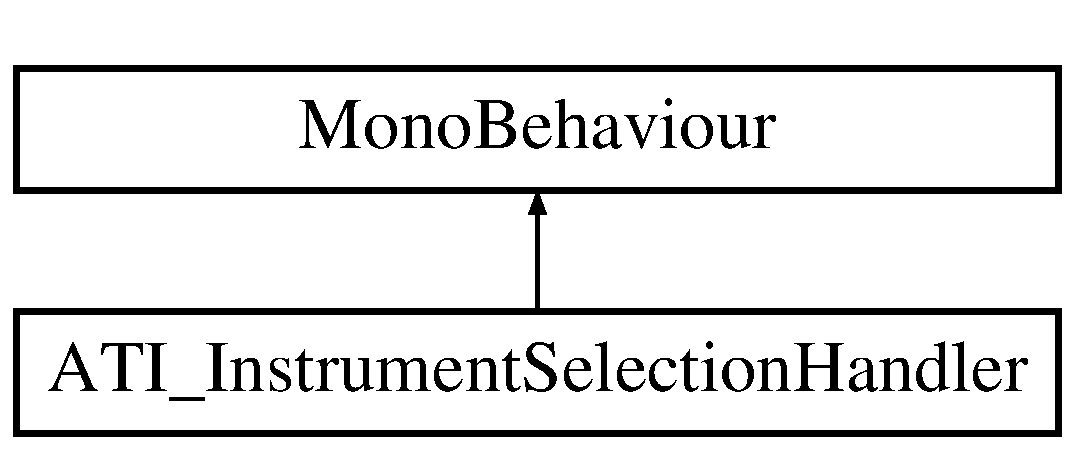
\includegraphics[height=2.000000cm]{class_a_t_i___instrument_selection_handler}
\end{center}
\end{figure}
\subsection*{Public Member Functions}
\begin{DoxyCompactItemize}
\item 
void \hyperlink{class_a_t_i___instrument_selection_handler_af9ac3dae1f7938a64d9ecdee529ee677}{On\+Instrument\+Selected} (int a\+Selection)
\end{DoxyCompactItemize}
\subsection*{Private Member Functions}
\begin{DoxyCompactItemize}
\item 
void \hyperlink{class_a_t_i___instrument_selection_handler_a5c6b182a8c8be5d409a2b17e6d8f67a2}{Start} ()
\item 
void \hyperlink{class_a_t_i___instrument_selection_handler_a725510a41c1f4665e3874029486aab99}{Update} ()
\end{DoxyCompactItemize}
\subsection*{Private Attributes}
\begin{DoxyCompactItemize}
\item 
\hyperlink{class_virtual_instrument_manager}{Virtual\+Instrument\+Manager} \hyperlink{class_a_t_i___instrument_selection_handler_a744213ecae613372020009bc5c9688c8}{m\+V\+IM} = null
\end{DoxyCompactItemize}


\subsection{Detailed Description}


Definition at line 14 of file A\+T\+I\+\_\+\+Instrument\+Selection\+Handler.\+cs.



\subsection{Member Function Documentation}
\mbox{\Hypertarget{class_a_t_i___instrument_selection_handler_af9ac3dae1f7938a64d9ecdee529ee677}\label{class_a_t_i___instrument_selection_handler_af9ac3dae1f7938a64d9ecdee529ee677}} 
\index{A\+T\+I\+\_\+\+Instrument\+Selection\+Handler@{A\+T\+I\+\_\+\+Instrument\+Selection\+Handler}!On\+Instrument\+Selected@{On\+Instrument\+Selected}}
\index{On\+Instrument\+Selected@{On\+Instrument\+Selected}!A\+T\+I\+\_\+\+Instrument\+Selection\+Handler@{A\+T\+I\+\_\+\+Instrument\+Selection\+Handler}}
\subsubsection{\texorpdfstring{On\+Instrument\+Selected()}{OnInstrumentSelected()}}
{\footnotesize\ttfamily void A\+T\+I\+\_\+\+Instrument\+Selection\+Handler.\+On\+Instrument\+Selected (\begin{DoxyParamCaption}\item[{int}]{a\+Selection }\end{DoxyParamCaption})}



Definition at line 58 of file A\+T\+I\+\_\+\+Instrument\+Selection\+Handler.\+cs.



References Virtual\+Instrument\+Manager.\+Change\+Instrument.


\begin{DoxyCode}
59     \{
60         \hyperlink{class_a_t_i___instrument_selection_handler_a744213ecae613372020009bc5c9688c8}{mVIM}.\hyperlink{group___v_i_m_events_ga1b9f12a73a5418ea5695d38b78c506c4}{ChangeInstrument}.Invoke( (\hyperlink{class_music}{Music}.
      \hyperlink{group___music_enums_gabfce60192305965558a36e368ebd67c3}{INSTRUMENT\_TYPE})aSelection );
61     \}
\end{DoxyCode}
\mbox{\Hypertarget{class_a_t_i___instrument_selection_handler_a5c6b182a8c8be5d409a2b17e6d8f67a2}\label{class_a_t_i___instrument_selection_handler_a5c6b182a8c8be5d409a2b17e6d8f67a2}} 
\index{A\+T\+I\+\_\+\+Instrument\+Selection\+Handler@{A\+T\+I\+\_\+\+Instrument\+Selection\+Handler}!Start@{Start}}
\index{Start@{Start}!A\+T\+I\+\_\+\+Instrument\+Selection\+Handler@{A\+T\+I\+\_\+\+Instrument\+Selection\+Handler}}
\subsubsection{\texorpdfstring{Start()}{Start()}}
{\footnotesize\ttfamily void A\+T\+I\+\_\+\+Instrument\+Selection\+Handler.\+Start (\begin{DoxyParamCaption}{ }\end{DoxyParamCaption})\hspace{0.3cm}{\ttfamily [private]}}



Definition at line 34 of file A\+T\+I\+\_\+\+Instrument\+Selection\+Handler.\+cs.


\begin{DoxyCode}
35     \{
36 
37 \textcolor{preprocessor}{#if DEBUG && DEBUG\_MUSICAL\_TYPING}
38         \hyperlink{class_a_t_i___instrument_selection_handler_a744213ecae613372020009bc5c9688c8}{mVIM} = GameObject.Find( \textcolor{stringliteral}{"VirtualInstrumentManager"} ).GetComponent<
      \hyperlink{class_virtual_instrument_manager}{VirtualInstrumentManager}>();
39 \textcolor{preprocessor}{#endif}
40 
41     \}
\end{DoxyCode}
\mbox{\Hypertarget{class_a_t_i___instrument_selection_handler_a725510a41c1f4665e3874029486aab99}\label{class_a_t_i___instrument_selection_handler_a725510a41c1f4665e3874029486aab99}} 
\index{A\+T\+I\+\_\+\+Instrument\+Selection\+Handler@{A\+T\+I\+\_\+\+Instrument\+Selection\+Handler}!Update@{Update}}
\index{Update@{Update}!A\+T\+I\+\_\+\+Instrument\+Selection\+Handler@{A\+T\+I\+\_\+\+Instrument\+Selection\+Handler}}
\subsubsection{\texorpdfstring{Update()}{Update()}}
{\footnotesize\ttfamily void A\+T\+I\+\_\+\+Instrument\+Selection\+Handler.\+Update (\begin{DoxyParamCaption}{ }\end{DoxyParamCaption})\hspace{0.3cm}{\ttfamily [private]}}



Definition at line 44 of file A\+T\+I\+\_\+\+Instrument\+Selection\+Handler.\+cs.


\begin{DoxyCode}
45     \{
46     \}
\end{DoxyCode}


\subsection{Member Data Documentation}
\mbox{\Hypertarget{class_a_t_i___instrument_selection_handler_a744213ecae613372020009bc5c9688c8}\label{class_a_t_i___instrument_selection_handler_a744213ecae613372020009bc5c9688c8}} 
\index{A\+T\+I\+\_\+\+Instrument\+Selection\+Handler@{A\+T\+I\+\_\+\+Instrument\+Selection\+Handler}!m\+V\+IM@{m\+V\+IM}}
\index{m\+V\+IM@{m\+V\+IM}!A\+T\+I\+\_\+\+Instrument\+Selection\+Handler@{A\+T\+I\+\_\+\+Instrument\+Selection\+Handler}}
\subsubsection{\texorpdfstring{m\+V\+IM}{mVIM}}
{\footnotesize\ttfamily \hyperlink{class_virtual_instrument_manager}{Virtual\+Instrument\+Manager} A\+T\+I\+\_\+\+Instrument\+Selection\+Handler.\+m\+V\+IM = null\hspace{0.3cm}{\ttfamily [private]}}



Definition at line 24 of file A\+T\+I\+\_\+\+Instrument\+Selection\+Handler.\+cs.



The documentation for this class was generated from the following file\+:\begin{DoxyCompactItemize}
\item 
D\+:/\+Documents/\+School Documents/2017\+Spring/\+E\+E\+C\+S542/\+V\+R\+Piano\+Project/\+Assets/\+Scripts/\+Audio/\+Testing/\hyperlink{_a_t_i___instrument_selection_handler_8cs}{A\+T\+I\+\_\+\+Instrument\+Selection\+Handler.\+cs}\end{DoxyCompactItemize}

\hypertarget{class_a_t_i___note_range_selection_handler}{}\section{A\+T\+I\+\_\+\+Note\+Range\+Selection\+Handler Class Reference}
\label{class_a_t_i___note_range_selection_handler}\index{A\+T\+I\+\_\+\+Note\+Range\+Selection\+Handler@{A\+T\+I\+\_\+\+Note\+Range\+Selection\+Handler}}
Inheritance diagram for A\+T\+I\+\_\+\+Note\+Range\+Selection\+Handler\+:\begin{figure}[H]
\begin{center}
\leavevmode
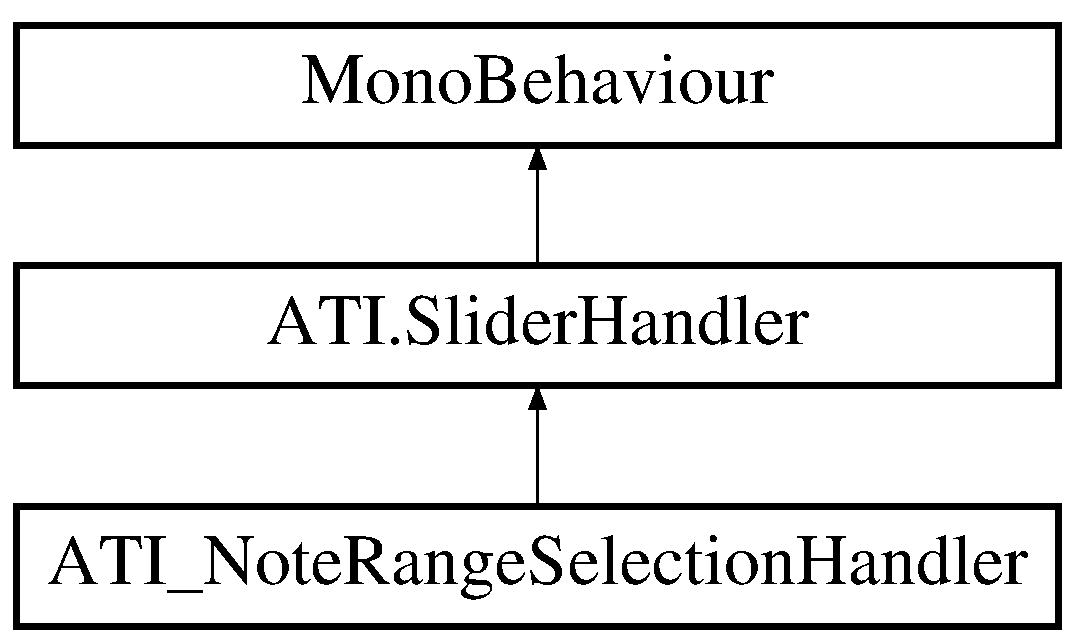
\includegraphics[height=3.000000cm]{class_a_t_i___note_range_selection_handler}
\end{center}
\end{figure}
\subsection*{Protected Member Functions}
\begin{DoxyCompactItemize}
\item 
override void \hyperlink{class_a_t_i___note_range_selection_handler_a87e90cac12626a0cb547d6e40c6e8260}{Handle\+Note\+Range\+Change} (bool a\+End\+Drag)
\end{DoxyCompactItemize}
\subsection*{Private Member Functions}
\begin{DoxyCompactItemize}
\item 
new void \hyperlink{class_a_t_i___note_range_selection_handler_a0840b64bb232377676cdb9cef62349f4}{Start} ()
\item 
void \hyperlink{class_a_t_i___note_range_selection_handler_ad1368483644433a2e1149790664676e8}{Update} ()
\item 
void \hyperlink{class_a_t_i___note_range_selection_handler_a4063aee2ca06e3fbe11f4cd899b5581f}{Handle\+Instrument\+Loaded} ()
\end{DoxyCompactItemize}
\subsection*{Additional Inherited Members}


\subsection{Detailed Description}


Definition at line 15 of file A\+T\+I\+\_\+\+Note\+Range\+Selection\+Handler.\+cs.



\subsection{Member Function Documentation}
\mbox{\Hypertarget{class_a_t_i___note_range_selection_handler_a4063aee2ca06e3fbe11f4cd899b5581f}\label{class_a_t_i___note_range_selection_handler_a4063aee2ca06e3fbe11f4cd899b5581f}} 
\index{A\+T\+I\+\_\+\+Note\+Range\+Selection\+Handler@{A\+T\+I\+\_\+\+Note\+Range\+Selection\+Handler}!Handle\+Instrument\+Loaded@{Handle\+Instrument\+Loaded}}
\index{Handle\+Instrument\+Loaded@{Handle\+Instrument\+Loaded}!A\+T\+I\+\_\+\+Note\+Range\+Selection\+Handler@{A\+T\+I\+\_\+\+Note\+Range\+Selection\+Handler}}
\subsubsection{\texorpdfstring{Handle\+Instrument\+Loaded()}{HandleInstrumentLoaded()}}
{\footnotesize\ttfamily void A\+T\+I\+\_\+\+Note\+Range\+Selection\+Handler.\+Handle\+Instrument\+Loaded (\begin{DoxyParamCaption}{ }\end{DoxyParamCaption})\hspace{0.3cm}{\ttfamily [private]}}



Definition at line 69 of file A\+T\+I\+\_\+\+Note\+Range\+Selection\+Handler.\+cs.



References Virtual\+Instrument\+Manager.\+Get\+Highest\+Supported\+Note(), Virtual\+Instrument\+Manager.\+Get\+Lowest\+Active\+Note(), Virtual\+Instrument\+Manager.\+Get\+Lowest\+Supported\+Note(), Virtual\+Instrument\+Manager.\+Get\+Num\+Active\+Notes(), A\+T\+I.\+Slider\+Handler.\+m\+Sliders, A\+T\+I.\+Slider\+Handler.\+m\+V\+IM, and Music.\+Note\+To\+String().



Referenced by Start().


\begin{DoxyCode}
70     \{
71         \textcolor{comment}{// Update the slider.}
72         \hyperlink{class_a_t_i_1_1_slider_handler_a038a487fbd701cb786e77c210830be76}{mSliders}[0].minValue = (float)\hyperlink{class_a_t_i_1_1_slider_handler_a5d19b4fb92b71c25a667defdda60213f}{mVIM}.\hyperlink{group___v_i_m_pub_func_gaeb152486450d6c6dc50078e1644c4c6a}{GetLowestSupportedNote}();
73         \hyperlink{class_a_t_i_1_1_slider_handler_a038a487fbd701cb786e77c210830be76}{mSliders}[0].maxValue = (float)( \hyperlink{class_a_t_i_1_1_slider_handler_a5d19b4fb92b71c25a667defdda60213f}{mVIM}.\hyperlink{group___v_i_m_pub_func_ga586d5ed5b0fe832d66c9a99aa160ceee}{GetHighestSupportedNote}() -
       \hyperlink{class_a_t_i_1_1_slider_handler_a5d19b4fb92b71c25a667defdda60213f}{mVIM}.\hyperlink{group___v_i_m_pub_func_ga3d6c823b1c1083eac8202f6c89e60b48}{GetNumActiveNotes}() + 1 );
74         \hyperlink{class_a_t_i_1_1_slider_handler_a038a487fbd701cb786e77c210830be76}{mSliders}[0].value = (float)\hyperlink{class_a_t_i_1_1_slider_handler_a5d19b4fb92b71c25a667defdda60213f}{mVIM}.\hyperlink{group___v_i_m_pub_func_ga09bfbd0756fc8110c877e5b59c104bcd}{GetLowestActiveNote}();
75 
76 
77 
78         \textcolor{comment}{// Update the slider text.}
79         \textcolor{comment}{// Set the text.}
80         gameObject.transform.GetChild( 3 ).GetComponent<Text>().text = \textcolor{stringliteral}{"Range: "} + 
      \hyperlink{class_music}{Music}.\hyperlink{group___music_stat_func_ga85a22c905d56d4c5f4e62159bfecee8c}{NoteToString}( (\textcolor{keywordtype}{int})\hyperlink{class_a_t_i_1_1_slider_handler_a038a487fbd701cb786e77c210830be76}{mSliders}[0].value )
81             + \textcolor{stringliteral}{" to "} + \hyperlink{class_music}{Music}.\hyperlink{group___music_stat_func_ga85a22c905d56d4c5f4e62159bfecee8c}{NoteToString}( (\textcolor{keywordtype}{int})mSliders[0].value + 
      \hyperlink{class_a_t_i_1_1_slider_handler_a5d19b4fb92b71c25a667defdda60213f}{mVIM}.\hyperlink{group___v_i_m_pub_func_ga3d6c823b1c1083eac8202f6c89e60b48}{GetNumActiveNotes}() - 1 );
82     \}
\end{DoxyCode}
\mbox{\Hypertarget{class_a_t_i___note_range_selection_handler_a87e90cac12626a0cb547d6e40c6e8260}\label{class_a_t_i___note_range_selection_handler_a87e90cac12626a0cb547d6e40c6e8260}} 
\index{A\+T\+I\+\_\+\+Note\+Range\+Selection\+Handler@{A\+T\+I\+\_\+\+Note\+Range\+Selection\+Handler}!Handle\+Note\+Range\+Change@{Handle\+Note\+Range\+Change}}
\index{Handle\+Note\+Range\+Change@{Handle\+Note\+Range\+Change}!A\+T\+I\+\_\+\+Note\+Range\+Selection\+Handler@{A\+T\+I\+\_\+\+Note\+Range\+Selection\+Handler}}
\subsubsection{\texorpdfstring{Handle\+Note\+Range\+Change()}{HandleNoteRangeChange()}}
{\footnotesize\ttfamily override void A\+T\+I\+\_\+\+Note\+Range\+Selection\+Handler.\+Handle\+Note\+Range\+Change (\begin{DoxyParamCaption}\item[{bool}]{a\+End\+Drag }\end{DoxyParamCaption})\hspace{0.3cm}{\ttfamily [protected]}, {\ttfamily [virtual]}}



Reimplemented from \hyperlink{class_a_t_i_1_1_slider_handler_a4d3915be92feddd4c45027a71c3a338c}{A\+T\+I.\+Slider\+Handler}.



Definition at line 56 of file A\+T\+I\+\_\+\+Note\+Range\+Selection\+Handler.\+cs.



References Virtual\+Instrument\+Manager.\+Change\+Note\+Range, Virtual\+Instrument\+Manager.\+Get\+Num\+Active\+Notes(), A\+T\+I.\+Slider\+Handler.\+m\+Sliders, A\+T\+I.\+Slider\+Handler.\+m\+V\+IM, and Music.\+Note\+To\+String().


\begin{DoxyCode}
57     \{
58         \textcolor{comment}{// Set the text.}
59         gameObject.transform.GetChild( 3 ).GetComponent<Text>().text = \textcolor{stringliteral}{"Range: "} + 
      \hyperlink{class_music}{Music}.\hyperlink{group___music_stat_func_ga85a22c905d56d4c5f4e62159bfecee8c}{NoteToString}( (\textcolor{keywordtype}{int})\hyperlink{class_a_t_i_1_1_slider_handler_a038a487fbd701cb786e77c210830be76}{mSliders}[0].value )
60             + \textcolor{stringliteral}{" to "} + \hyperlink{class_music}{Music}.\hyperlink{group___music_stat_func_ga85a22c905d56d4c5f4e62159bfecee8c}{NoteToString}( (\textcolor{keywordtype}{int})mSliders[0].value + 
      \hyperlink{class_a_t_i_1_1_slider_handler_a5d19b4fb92b71c25a667defdda60213f}{mVIM}.\hyperlink{group___v_i_m_pub_func_ga3d6c823b1c1083eac8202f6c89e60b48}{GetNumActiveNotes}() - 1 );
61 
62         \textcolor{comment}{// If the value has been set, then invoke the virtual instrument manager's ChangeNoteRange event.}
63         \textcolor{keywordflow}{if}( aEndDrag )
64         \{
65             \hyperlink{class_a_t_i_1_1_slider_handler_a5d19b4fb92b71c25a667defdda60213f}{mVIM}.\hyperlink{group___v_i_m_events_gab6fa99d08e8466406835b9fc4ff859f1}{ChangeNoteRange}.Invoke( (\hyperlink{class_music}{Music}.\hyperlink{group___music_enums_ga508f69b199ea518f935486c990edac1d}{PITCH})mSliders[0].value );
66         \}
67     \}
\end{DoxyCode}
\mbox{\Hypertarget{class_a_t_i___note_range_selection_handler_a0840b64bb232377676cdb9cef62349f4}\label{class_a_t_i___note_range_selection_handler_a0840b64bb232377676cdb9cef62349f4}} 
\index{A\+T\+I\+\_\+\+Note\+Range\+Selection\+Handler@{A\+T\+I\+\_\+\+Note\+Range\+Selection\+Handler}!Start@{Start}}
\index{Start@{Start}!A\+T\+I\+\_\+\+Note\+Range\+Selection\+Handler@{A\+T\+I\+\_\+\+Note\+Range\+Selection\+Handler}}
\subsubsection{\texorpdfstring{Start()}{Start()}}
{\footnotesize\ttfamily new void A\+T\+I\+\_\+\+Note\+Range\+Selection\+Handler.\+Start (\begin{DoxyParamCaption}{ }\end{DoxyParamCaption})\hspace{0.3cm}{\ttfamily [private]}}



Definition at line 23 of file A\+T\+I\+\_\+\+Note\+Range\+Selection\+Handler.\+cs.



References Handle\+Instrument\+Loaded(), Virtual\+Instrument\+Manager.\+Instrument\+Loaded, A\+T\+I.\+Slider\+Handler.\+m\+Sliders, A\+T\+I.\+Slider\+Handler.\+m\+V\+IM, and A\+T\+I.\+Slider\+Trigger.\+Set\+Handler().


\begin{DoxyCode}
24     \{
25 
26 \textcolor{preprocessor}{#if DEBUG && DEBUG\_MUSICAL\_TYPING}
27 
28         \textcolor{comment}{// Call the base start function.}
29         base.Start();
30 
31         \textcolor{comment}{// Get the slider and set up its trigger}
32         \hyperlink{class_a_t_i}{ATI}.\hyperlink{class_a_t_i_1_1_slider_trigger}{SliderTrigger} st = null;
33         \hyperlink{class_a_t_i_1_1_slider_handler_a038a487fbd701cb786e77c210830be76}{mSliders} = \textcolor{keyword}{new} Slider[1];
34         \hyperlink{class_a_t_i_1_1_slider_handler_a038a487fbd701cb786e77c210830be76}{mSliders}[0] = gameObject.transform.GetComponent<Slider>();
35         st = \hyperlink{class_a_t_i_1_1_slider_handler_a038a487fbd701cb786e77c210830be76}{mSliders}[0].gameObject.AddComponent<\hyperlink{class_a_t_i}{ATI}.\hyperlink{class_a_t_i_1_1_slider_trigger}{SliderTrigger}>();
36         st.\hyperlink{class_a_t_i_1_1_slider_trigger_a258f79d013266d0c82a5382525adcdef}{SetHandler}( \textcolor{keyword}{this} );
37         st.SetType( \hyperlink{class_a_t_i}{ATI}.\hyperlink{class_a_t_i_ac4c6056a99cbd16ff0d292d33b038b9b}{SliderType}.NoteRange );
38 
39         \hyperlink{class_a_t_i_1_1_slider_handler_a5d19b4fb92b71c25a667defdda60213f}{mVIM}.\hyperlink{group___v_i_m_events_gad79b789b020d7e4a8c149ec653c0b97f}{InstrumentLoaded}.AddListener( 
      \hyperlink{class_a_t_i___note_range_selection_handler_a4063aee2ca06e3fbe11f4cd899b5581f}{HandleInstrumentLoaded} );
40 \textcolor{preprocessor}{#endif}
41 
42     \}
\end{DoxyCode}
\mbox{\Hypertarget{class_a_t_i___note_range_selection_handler_ad1368483644433a2e1149790664676e8}\label{class_a_t_i___note_range_selection_handler_ad1368483644433a2e1149790664676e8}} 
\index{A\+T\+I\+\_\+\+Note\+Range\+Selection\+Handler@{A\+T\+I\+\_\+\+Note\+Range\+Selection\+Handler}!Update@{Update}}
\index{Update@{Update}!A\+T\+I\+\_\+\+Note\+Range\+Selection\+Handler@{A\+T\+I\+\_\+\+Note\+Range\+Selection\+Handler}}
\subsubsection{\texorpdfstring{Update()}{Update()}}
{\footnotesize\ttfamily void A\+T\+I\+\_\+\+Note\+Range\+Selection\+Handler.\+Update (\begin{DoxyParamCaption}{ }\end{DoxyParamCaption})\hspace{0.3cm}{\ttfamily [private]}}



Definition at line 45 of file A\+T\+I\+\_\+\+Note\+Range\+Selection\+Handler.\+cs.


\begin{DoxyCode}
46     \{
47 
48     \}
\end{DoxyCode}


The documentation for this class was generated from the following file\+:\begin{DoxyCompactItemize}
\item 
D\+:/\+Documents/\+School Documents/2017\+Spring/\+E\+E\+C\+S542/\+V\+R\+Piano\+Project/\+Assets/\+Scripts/\+Audio/\+Testing/\hyperlink{_a_t_i___note_range_selection_handler_8cs}{A\+T\+I\+\_\+\+Note\+Range\+Selection\+Handler.\+cs}\end{DoxyCompactItemize}

\hypertarget{class_a_t_i___reverb_filter_handler}{}\section{A\+T\+I\+\_\+\+Reverb\+Filter\+Handler Class Reference}
\label{class_a_t_i___reverb_filter_handler}\index{A\+T\+I\+\_\+\+Reverb\+Filter\+Handler@{A\+T\+I\+\_\+\+Reverb\+Filter\+Handler}}
Inheritance diagram for A\+T\+I\+\_\+\+Reverb\+Filter\+Handler\+:\begin{figure}[H]
\begin{center}
\leavevmode
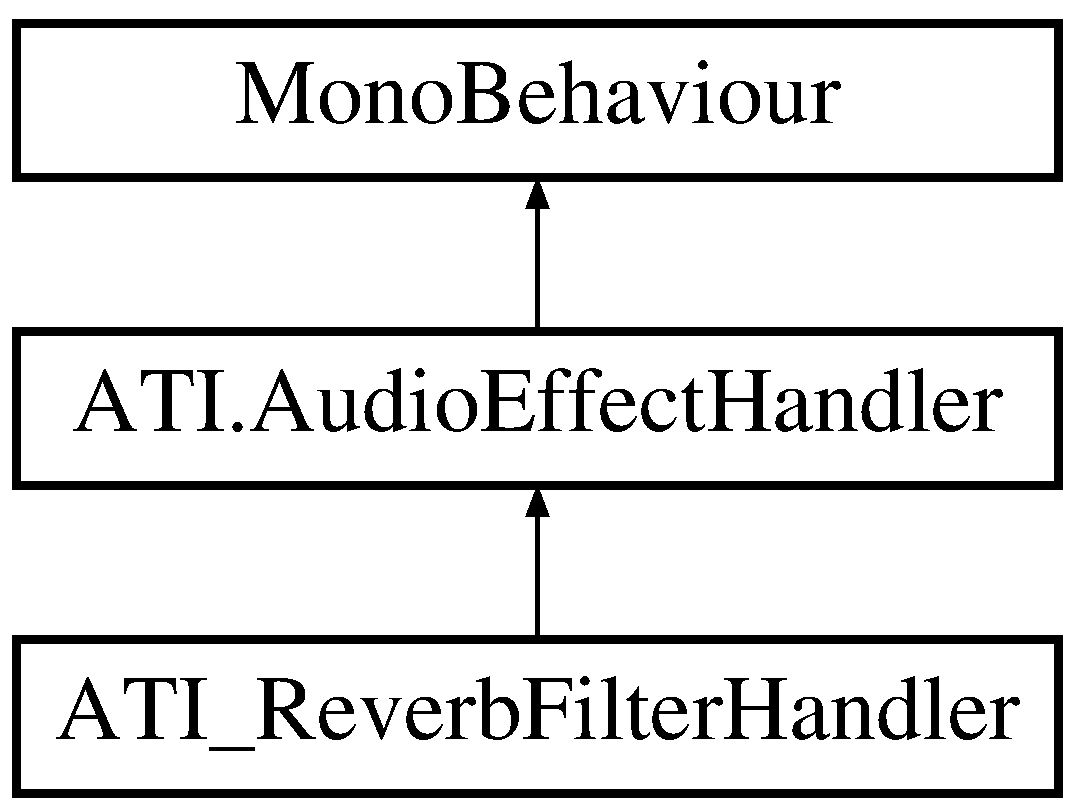
\includegraphics[height=3.000000cm]{class_a_t_i___reverb_filter_handler}
\end{center}
\end{figure}
\subsection*{Protected Member Functions}
\begin{DoxyCompactItemize}
\item 
override void \hyperlink{class_a_t_i___reverb_filter_handler_a69a75dcda06ae1597030e0ceaf84e1ae}{Set\+Default\+Parameters} ()
\item 
override void \hyperlink{class_a_t_i___reverb_filter_handler_aacb469dc3038fca616d638f6a5a04a30}{Send\+Parameters\+To\+V\+IM} ()
\item 
override void \hyperlink{class_a_t_i___reverb_filter_handler_aa25fcaa9c07d614b869334e1db14f7d6}{Turn\+On\+Effect} ()
\item 
override void \hyperlink{class_a_t_i___reverb_filter_handler_a87b5c207c0ec0422ce8bea66a38334e2}{Turn\+Off\+Effect} ()
\item 
override void \hyperlink{class_a_t_i___reverb_filter_handler_a084dca3566139f350b0372d3ee85af84}{Handle\+Scene\+Load} ()
\item 
override void \hyperlink{class_a_t_i___reverb_filter_handler_a0af6a4381b725183fdb7cc8589a9f71f}{Handle\+Dry\+Level\+Change} (float a\+Value)
\item 
override void \hyperlink{class_a_t_i___reverb_filter_handler_a2100456086ad1adf704bf88d71dbe490}{Handle\+Room\+Change} (float a\+Value)
\item 
override void \hyperlink{class_a_t_i___reverb_filter_handler_a587ab9596231ed2ff9e3628bbc59d510}{Handle\+Room\+H\+F\+Change} (float a\+Value)
\item 
override void \hyperlink{class_a_t_i___reverb_filter_handler_a30a45fb9d8bbd7e10054eaa4595666b3}{Handle\+Decay\+Time\+Change} (float a\+Value)
\item 
override void \hyperlink{class_a_t_i___reverb_filter_handler_a68dab792c963c33be3618c9595a6a734}{Handle\+Decay\+H\+F\+Ratio\+Change} (float a\+Value)
\item 
override void \hyperlink{class_a_t_i___reverb_filter_handler_a8db38f7eafd2b1ed0a5f8d488244d83a}{Handle\+Reflections\+Change} (float a\+Value)
\item 
override void \hyperlink{class_a_t_i___reverb_filter_handler_a83de9c38851424d66456dfe98163dfde}{Handle\+Reflect\+Delay\+Change} (float a\+Value)
\item 
override void \hyperlink{class_a_t_i___reverb_filter_handler_ae228f1d67c8efd950a3b2c594d5dd9f8}{Handle\+Reverb\+Change} (float a\+Value)
\item 
override void \hyperlink{class_a_t_i___reverb_filter_handler_af126757d50b12330f868d2178bdb5d6c}{Handle\+Reverb\+Delay\+Change} (float a\+Value)
\item 
override void \hyperlink{class_a_t_i___reverb_filter_handler_a6cd79af5d1835bd4ab8a6420fed82e53}{Handle\+Diffusion\+Change} (float a\+Value)
\item 
override void \hyperlink{class_a_t_i___reverb_filter_handler_a4a95ee1076720663fbe84e624385e636}{Handle\+Density\+Change} (float a\+Value)
\item 
override void \hyperlink{class_a_t_i___reverb_filter_handler_a4cb8ab454ef637beb189053a0877c8c6}{Handle\+H\+F\+Reference\+Change} (float a\+Value)
\item 
override void \hyperlink{class_a_t_i___reverb_filter_handler_a52fe6f9775f8e51296580f7a96b47bdb}{Handle\+Room\+L\+F\+Change} (float a\+Value)
\item 
override void \hyperlink{class_a_t_i___reverb_filter_handler_abf697e814be89c3bd354deaccb237746}{Handle\+L\+F\+Reference\+Change} (float a\+Value)
\end{DoxyCompactItemize}
\subsection*{Private Member Functions}
\begin{DoxyCompactItemize}
\item 
new void \hyperlink{class_a_t_i___reverb_filter_handler_af9e294ce4222c0e564ea864c14106e7e}{Start} ()
\end{DoxyCompactItemize}
\subsection*{Private Attributes}
\begin{DoxyCompactItemize}
\item 
Game\+Object \hyperlink{class_a_t_i___reverb_filter_handler_a1373be0e7de8911f4e95f10289117389}{m\+Dry\+Level\+Container} = null
\item 
Game\+Object \hyperlink{class_a_t_i___reverb_filter_handler_aba031a396792257ab91bd8fc56a3c402}{m\+Room\+Container} = null
\item 
Game\+Object \hyperlink{class_a_t_i___reverb_filter_handler_a87b996d08d23419b6403347ca0316daf}{m\+Room\+H\+F\+Container} = null
\item 
Game\+Object \hyperlink{class_a_t_i___reverb_filter_handler_a797cdcbb421ba074802a553047cce07e}{m\+Decay\+Time\+Container} = null
\item 
Game\+Object \hyperlink{class_a_t_i___reverb_filter_handler_a747b42c6663dae5892048cc714677101}{m\+Decay\+H\+F\+Ratio\+Container} = null
\item 
Game\+Object \hyperlink{class_a_t_i___reverb_filter_handler_a03319a2f6cc8e26f074789fb525584e7}{m\+Reflections\+Container} = null
\item 
Game\+Object \hyperlink{class_a_t_i___reverb_filter_handler_a8344d44e118de9b321cdf0b84a383f89}{m\+Reflect\+Delay\+Container} = null
\item 
Game\+Object \hyperlink{class_a_t_i___reverb_filter_handler_a8af547f0f1c566b57439d4ec5ce244b4}{m\+Reverb\+Container} = null
\item 
Game\+Object \hyperlink{class_a_t_i___reverb_filter_handler_affa45d12ae5c3f25f8662fca54dc6bbe}{m\+Reverb\+Delay\+Container} = null
\item 
Game\+Object \hyperlink{class_a_t_i___reverb_filter_handler_a68deedceca43c3fc45ee80912e4c8fa7}{m\+Diffusion\+Container} = null
\item 
Game\+Object \hyperlink{class_a_t_i___reverb_filter_handler_a1668ae518533eee4658e3bc65e377491}{m\+Density\+Container} = null
\item 
Game\+Object \hyperlink{class_a_t_i___reverb_filter_handler_a45c18f64f4e32e59580246305ba785ae}{m\+H\+F\+Reference\+Container} = null
\item 
Game\+Object \hyperlink{class_a_t_i___reverb_filter_handler_ab29f45ffbe20f9f44305f3f009c8fa6b}{m\+Room\+L\+F\+Container} = null
\item 
Game\+Object \hyperlink{class_a_t_i___reverb_filter_handler_ae9010ffdcbb124b62027df7d31feeecb}{m\+L\+F\+Reference\+Container} = null
\item 
\hyperlink{group__filter_params_struct_virtual_instrument_manager_1_1_reverb_filter_parameters}{Virtual\+Instrument\+Manager.\+Reverb\+Filter\+Parameters} \hyperlink{class_a_t_i___reverb_filter_handler_a034260fbce2052b42bceddc891632347}{m\+Params}
\end{DoxyCompactItemize}
\subsection*{Additional Inherited Members}


\subsection{Detailed Description}


Definition at line 16 of file A\+T\+I\+\_\+\+Reverb\+Filter\+Handler.\+cs.



\subsection{Member Function Documentation}
\mbox{\Hypertarget{class_a_t_i___reverb_filter_handler_a68dab792c963c33be3618c9595a6a734}\label{class_a_t_i___reverb_filter_handler_a68dab792c963c33be3618c9595a6a734}} 
\index{A\+T\+I\+\_\+\+Reverb\+Filter\+Handler@{A\+T\+I\+\_\+\+Reverb\+Filter\+Handler}!Handle\+Decay\+H\+F\+Ratio\+Change@{Handle\+Decay\+H\+F\+Ratio\+Change}}
\index{Handle\+Decay\+H\+F\+Ratio\+Change@{Handle\+Decay\+H\+F\+Ratio\+Change}!A\+T\+I\+\_\+\+Reverb\+Filter\+Handler@{A\+T\+I\+\_\+\+Reverb\+Filter\+Handler}}
\subsubsection{\texorpdfstring{Handle\+Decay\+H\+F\+Ratio\+Change()}{HandleDecayHFRatioChange()}}
{\footnotesize\ttfamily override void A\+T\+I\+\_\+\+Reverb\+Filter\+Handler.\+Handle\+Decay\+H\+F\+Ratio\+Change (\begin{DoxyParamCaption}\item[{float}]{a\+Value }\end{DoxyParamCaption})\hspace{0.3cm}{\ttfamily [protected]}, {\ttfamily [virtual]}}



Reimplemented from \hyperlink{class_a_t_i_1_1_audio_effect_handler_af00cbc35b44d68de0d2d0497e1defa3a}{A\+T\+I.\+Audio\+Effect\+Handler}.



Definition at line 295 of file A\+T\+I\+\_\+\+Reverb\+Filter\+Handler.\+cs.



References m\+Params, and Send\+Parameters\+To\+V\+I\+M().


\begin{DoxyCode}
296     \{
297         \hyperlink{class_a_t_i___reverb_filter_handler_a034260fbce2052b42bceddc891632347}{mParams}.DecayHFRatio = aValue;
298         \hyperlink{class_a_t_i___reverb_filter_handler_aacb469dc3038fca616d638f6a5a04a30}{SendParametersToVIM}();
299     \}
\end{DoxyCode}
\mbox{\Hypertarget{class_a_t_i___reverb_filter_handler_a30a45fb9d8bbd7e10054eaa4595666b3}\label{class_a_t_i___reverb_filter_handler_a30a45fb9d8bbd7e10054eaa4595666b3}} 
\index{A\+T\+I\+\_\+\+Reverb\+Filter\+Handler@{A\+T\+I\+\_\+\+Reverb\+Filter\+Handler}!Handle\+Decay\+Time\+Change@{Handle\+Decay\+Time\+Change}}
\index{Handle\+Decay\+Time\+Change@{Handle\+Decay\+Time\+Change}!A\+T\+I\+\_\+\+Reverb\+Filter\+Handler@{A\+T\+I\+\_\+\+Reverb\+Filter\+Handler}}
\subsubsection{\texorpdfstring{Handle\+Decay\+Time\+Change()}{HandleDecayTimeChange()}}
{\footnotesize\ttfamily override void A\+T\+I\+\_\+\+Reverb\+Filter\+Handler.\+Handle\+Decay\+Time\+Change (\begin{DoxyParamCaption}\item[{float}]{a\+Value }\end{DoxyParamCaption})\hspace{0.3cm}{\ttfamily [protected]}, {\ttfamily [virtual]}}



Reimplemented from \hyperlink{class_a_t_i_1_1_audio_effect_handler_a35173ee088bc2459907af3521bcd69ac}{A\+T\+I.\+Audio\+Effect\+Handler}.



Definition at line 287 of file A\+T\+I\+\_\+\+Reverb\+Filter\+Handler.\+cs.



References m\+Params, and Send\+Parameters\+To\+V\+I\+M().


\begin{DoxyCode}
288     \{
289         \hyperlink{class_a_t_i___reverb_filter_handler_a034260fbce2052b42bceddc891632347}{mParams}.DecayTime = aValue;
290         \hyperlink{class_a_t_i___reverb_filter_handler_aacb469dc3038fca616d638f6a5a04a30}{SendParametersToVIM}();
291     \}
\end{DoxyCode}
\mbox{\Hypertarget{class_a_t_i___reverb_filter_handler_a4a95ee1076720663fbe84e624385e636}\label{class_a_t_i___reverb_filter_handler_a4a95ee1076720663fbe84e624385e636}} 
\index{A\+T\+I\+\_\+\+Reverb\+Filter\+Handler@{A\+T\+I\+\_\+\+Reverb\+Filter\+Handler}!Handle\+Density\+Change@{Handle\+Density\+Change}}
\index{Handle\+Density\+Change@{Handle\+Density\+Change}!A\+T\+I\+\_\+\+Reverb\+Filter\+Handler@{A\+T\+I\+\_\+\+Reverb\+Filter\+Handler}}
\subsubsection{\texorpdfstring{Handle\+Density\+Change()}{HandleDensityChange()}}
{\footnotesize\ttfamily override void A\+T\+I\+\_\+\+Reverb\+Filter\+Handler.\+Handle\+Density\+Change (\begin{DoxyParamCaption}\item[{float}]{a\+Value }\end{DoxyParamCaption})\hspace{0.3cm}{\ttfamily [protected]}, {\ttfamily [virtual]}}



Reimplemented from \hyperlink{class_a_t_i_1_1_audio_effect_handler_acdbfbd384e2fdb5bd43ad977e264500a}{A\+T\+I.\+Audio\+Effect\+Handler}.



Definition at line 343 of file A\+T\+I\+\_\+\+Reverb\+Filter\+Handler.\+cs.



References m\+Params, and Send\+Parameters\+To\+V\+I\+M().


\begin{DoxyCode}
344     \{
345         \hyperlink{class_a_t_i___reverb_filter_handler_a034260fbce2052b42bceddc891632347}{mParams}.Density = aValue;
346         \hyperlink{class_a_t_i___reverb_filter_handler_aacb469dc3038fca616d638f6a5a04a30}{SendParametersToVIM}();
347     \}
\end{DoxyCode}
\mbox{\Hypertarget{class_a_t_i___reverb_filter_handler_a6cd79af5d1835bd4ab8a6420fed82e53}\label{class_a_t_i___reverb_filter_handler_a6cd79af5d1835bd4ab8a6420fed82e53}} 
\index{A\+T\+I\+\_\+\+Reverb\+Filter\+Handler@{A\+T\+I\+\_\+\+Reverb\+Filter\+Handler}!Handle\+Diffusion\+Change@{Handle\+Diffusion\+Change}}
\index{Handle\+Diffusion\+Change@{Handle\+Diffusion\+Change}!A\+T\+I\+\_\+\+Reverb\+Filter\+Handler@{A\+T\+I\+\_\+\+Reverb\+Filter\+Handler}}
\subsubsection{\texorpdfstring{Handle\+Diffusion\+Change()}{HandleDiffusionChange()}}
{\footnotesize\ttfamily override void A\+T\+I\+\_\+\+Reverb\+Filter\+Handler.\+Handle\+Diffusion\+Change (\begin{DoxyParamCaption}\item[{float}]{a\+Value }\end{DoxyParamCaption})\hspace{0.3cm}{\ttfamily [protected]}, {\ttfamily [virtual]}}



Reimplemented from \hyperlink{class_a_t_i_1_1_audio_effect_handler_adcf777de620420b6c411350db0eca2aa}{A\+T\+I.\+Audio\+Effect\+Handler}.



Definition at line 335 of file A\+T\+I\+\_\+\+Reverb\+Filter\+Handler.\+cs.



References m\+Params, and Send\+Parameters\+To\+V\+I\+M().


\begin{DoxyCode}
336     \{
337         \hyperlink{class_a_t_i___reverb_filter_handler_a034260fbce2052b42bceddc891632347}{mParams}.Diffusion = aValue;
338         \hyperlink{class_a_t_i___reverb_filter_handler_aacb469dc3038fca616d638f6a5a04a30}{SendParametersToVIM}();
339     \}
\end{DoxyCode}
\mbox{\Hypertarget{class_a_t_i___reverb_filter_handler_a0af6a4381b725183fdb7cc8589a9f71f}\label{class_a_t_i___reverb_filter_handler_a0af6a4381b725183fdb7cc8589a9f71f}} 
\index{A\+T\+I\+\_\+\+Reverb\+Filter\+Handler@{A\+T\+I\+\_\+\+Reverb\+Filter\+Handler}!Handle\+Dry\+Level\+Change@{Handle\+Dry\+Level\+Change}}
\index{Handle\+Dry\+Level\+Change@{Handle\+Dry\+Level\+Change}!A\+T\+I\+\_\+\+Reverb\+Filter\+Handler@{A\+T\+I\+\_\+\+Reverb\+Filter\+Handler}}
\subsubsection{\texorpdfstring{Handle\+Dry\+Level\+Change()}{HandleDryLevelChange()}}
{\footnotesize\ttfamily override void A\+T\+I\+\_\+\+Reverb\+Filter\+Handler.\+Handle\+Dry\+Level\+Change (\begin{DoxyParamCaption}\item[{float}]{a\+Value }\end{DoxyParamCaption})\hspace{0.3cm}{\ttfamily [protected]}, {\ttfamily [virtual]}}



Reimplemented from \hyperlink{class_a_t_i_1_1_audio_effect_handler_abf6b4a6ead7e60bbaea15f94936c316e}{A\+T\+I.\+Audio\+Effect\+Handler}.



Definition at line 263 of file A\+T\+I\+\_\+\+Reverb\+Filter\+Handler.\+cs.



References m\+Params, and Send\+Parameters\+To\+V\+I\+M().


\begin{DoxyCode}
264     \{
265         \hyperlink{class_a_t_i___reverb_filter_handler_a034260fbce2052b42bceddc891632347}{mParams}.DryLevel = aValue;
266         \hyperlink{class_a_t_i___reverb_filter_handler_aacb469dc3038fca616d638f6a5a04a30}{SendParametersToVIM}();
267     \}
\end{DoxyCode}
\mbox{\Hypertarget{class_a_t_i___reverb_filter_handler_a4cb8ab454ef637beb189053a0877c8c6}\label{class_a_t_i___reverb_filter_handler_a4cb8ab454ef637beb189053a0877c8c6}} 
\index{A\+T\+I\+\_\+\+Reverb\+Filter\+Handler@{A\+T\+I\+\_\+\+Reverb\+Filter\+Handler}!Handle\+H\+F\+Reference\+Change@{Handle\+H\+F\+Reference\+Change}}
\index{Handle\+H\+F\+Reference\+Change@{Handle\+H\+F\+Reference\+Change}!A\+T\+I\+\_\+\+Reverb\+Filter\+Handler@{A\+T\+I\+\_\+\+Reverb\+Filter\+Handler}}
\subsubsection{\texorpdfstring{Handle\+H\+F\+Reference\+Change()}{HandleHFReferenceChange()}}
{\footnotesize\ttfamily override void A\+T\+I\+\_\+\+Reverb\+Filter\+Handler.\+Handle\+H\+F\+Reference\+Change (\begin{DoxyParamCaption}\item[{float}]{a\+Value }\end{DoxyParamCaption})\hspace{0.3cm}{\ttfamily [protected]}, {\ttfamily [virtual]}}



Reimplemented from \hyperlink{class_a_t_i_1_1_audio_effect_handler_a183b75c93279e0d6322a0e005c590891}{A\+T\+I.\+Audio\+Effect\+Handler}.



Definition at line 351 of file A\+T\+I\+\_\+\+Reverb\+Filter\+Handler.\+cs.



References m\+Params, and Send\+Parameters\+To\+V\+I\+M().


\begin{DoxyCode}
352     \{
353         \hyperlink{class_a_t_i___reverb_filter_handler_a034260fbce2052b42bceddc891632347}{mParams}.HFReference = aValue;
354         \hyperlink{class_a_t_i___reverb_filter_handler_aacb469dc3038fca616d638f6a5a04a30}{SendParametersToVIM}();
355     \}
\end{DoxyCode}
\mbox{\Hypertarget{class_a_t_i___reverb_filter_handler_abf697e814be89c3bd354deaccb237746}\label{class_a_t_i___reverb_filter_handler_abf697e814be89c3bd354deaccb237746}} 
\index{A\+T\+I\+\_\+\+Reverb\+Filter\+Handler@{A\+T\+I\+\_\+\+Reverb\+Filter\+Handler}!Handle\+L\+F\+Reference\+Change@{Handle\+L\+F\+Reference\+Change}}
\index{Handle\+L\+F\+Reference\+Change@{Handle\+L\+F\+Reference\+Change}!A\+T\+I\+\_\+\+Reverb\+Filter\+Handler@{A\+T\+I\+\_\+\+Reverb\+Filter\+Handler}}
\subsubsection{\texorpdfstring{Handle\+L\+F\+Reference\+Change()}{HandleLFReferenceChange()}}
{\footnotesize\ttfamily override void A\+T\+I\+\_\+\+Reverb\+Filter\+Handler.\+Handle\+L\+F\+Reference\+Change (\begin{DoxyParamCaption}\item[{float}]{a\+Value }\end{DoxyParamCaption})\hspace{0.3cm}{\ttfamily [protected]}, {\ttfamily [virtual]}}



Reimplemented from \hyperlink{class_a_t_i_1_1_audio_effect_handler_a8414b47429880ba18133571c86cf14ab}{A\+T\+I.\+Audio\+Effect\+Handler}.



Definition at line 367 of file A\+T\+I\+\_\+\+Reverb\+Filter\+Handler.\+cs.



References m\+Params, and Send\+Parameters\+To\+V\+I\+M().


\begin{DoxyCode}
368     \{
369         \hyperlink{class_a_t_i___reverb_filter_handler_a034260fbce2052b42bceddc891632347}{mParams}.LFReference = aValue;
370         \hyperlink{class_a_t_i___reverb_filter_handler_aacb469dc3038fca616d638f6a5a04a30}{SendParametersToVIM}();
371     \}
\end{DoxyCode}
\mbox{\Hypertarget{class_a_t_i___reverb_filter_handler_a83de9c38851424d66456dfe98163dfde}\label{class_a_t_i___reverb_filter_handler_a83de9c38851424d66456dfe98163dfde}} 
\index{A\+T\+I\+\_\+\+Reverb\+Filter\+Handler@{A\+T\+I\+\_\+\+Reverb\+Filter\+Handler}!Handle\+Reflect\+Delay\+Change@{Handle\+Reflect\+Delay\+Change}}
\index{Handle\+Reflect\+Delay\+Change@{Handle\+Reflect\+Delay\+Change}!A\+T\+I\+\_\+\+Reverb\+Filter\+Handler@{A\+T\+I\+\_\+\+Reverb\+Filter\+Handler}}
\subsubsection{\texorpdfstring{Handle\+Reflect\+Delay\+Change()}{HandleReflectDelayChange()}}
{\footnotesize\ttfamily override void A\+T\+I\+\_\+\+Reverb\+Filter\+Handler.\+Handle\+Reflect\+Delay\+Change (\begin{DoxyParamCaption}\item[{float}]{a\+Value }\end{DoxyParamCaption})\hspace{0.3cm}{\ttfamily [protected]}, {\ttfamily [virtual]}}



Reimplemented from \hyperlink{class_a_t_i_1_1_audio_effect_handler_ada336ed04fdb3360de3026ba8659c409}{A\+T\+I.\+Audio\+Effect\+Handler}.



Definition at line 311 of file A\+T\+I\+\_\+\+Reverb\+Filter\+Handler.\+cs.



References m\+Params, and Send\+Parameters\+To\+V\+I\+M().


\begin{DoxyCode}
312     \{
313         \hyperlink{class_a_t_i___reverb_filter_handler_a034260fbce2052b42bceddc891632347}{mParams}.ReflectDelay = aValue;
314         \hyperlink{class_a_t_i___reverb_filter_handler_aacb469dc3038fca616d638f6a5a04a30}{SendParametersToVIM}();
315     \}
\end{DoxyCode}
\mbox{\Hypertarget{class_a_t_i___reverb_filter_handler_a8db38f7eafd2b1ed0a5f8d488244d83a}\label{class_a_t_i___reverb_filter_handler_a8db38f7eafd2b1ed0a5f8d488244d83a}} 
\index{A\+T\+I\+\_\+\+Reverb\+Filter\+Handler@{A\+T\+I\+\_\+\+Reverb\+Filter\+Handler}!Handle\+Reflections\+Change@{Handle\+Reflections\+Change}}
\index{Handle\+Reflections\+Change@{Handle\+Reflections\+Change}!A\+T\+I\+\_\+\+Reverb\+Filter\+Handler@{A\+T\+I\+\_\+\+Reverb\+Filter\+Handler}}
\subsubsection{\texorpdfstring{Handle\+Reflections\+Change()}{HandleReflectionsChange()}}
{\footnotesize\ttfamily override void A\+T\+I\+\_\+\+Reverb\+Filter\+Handler.\+Handle\+Reflections\+Change (\begin{DoxyParamCaption}\item[{float}]{a\+Value }\end{DoxyParamCaption})\hspace{0.3cm}{\ttfamily [protected]}, {\ttfamily [virtual]}}



Reimplemented from \hyperlink{class_a_t_i_1_1_audio_effect_handler_af50ba52dba236a3b711172fd6bbc1bab}{A\+T\+I.\+Audio\+Effect\+Handler}.



Definition at line 303 of file A\+T\+I\+\_\+\+Reverb\+Filter\+Handler.\+cs.



References m\+Params, and Send\+Parameters\+To\+V\+I\+M().


\begin{DoxyCode}
304     \{
305         \hyperlink{class_a_t_i___reverb_filter_handler_a034260fbce2052b42bceddc891632347}{mParams}.Reflections = aValue;
306         \hyperlink{class_a_t_i___reverb_filter_handler_aacb469dc3038fca616d638f6a5a04a30}{SendParametersToVIM}();
307     \}
\end{DoxyCode}
\mbox{\Hypertarget{class_a_t_i___reverb_filter_handler_ae228f1d67c8efd950a3b2c594d5dd9f8}\label{class_a_t_i___reverb_filter_handler_ae228f1d67c8efd950a3b2c594d5dd9f8}} 
\index{A\+T\+I\+\_\+\+Reverb\+Filter\+Handler@{A\+T\+I\+\_\+\+Reverb\+Filter\+Handler}!Handle\+Reverb\+Change@{Handle\+Reverb\+Change}}
\index{Handle\+Reverb\+Change@{Handle\+Reverb\+Change}!A\+T\+I\+\_\+\+Reverb\+Filter\+Handler@{A\+T\+I\+\_\+\+Reverb\+Filter\+Handler}}
\subsubsection{\texorpdfstring{Handle\+Reverb\+Change()}{HandleReverbChange()}}
{\footnotesize\ttfamily override void A\+T\+I\+\_\+\+Reverb\+Filter\+Handler.\+Handle\+Reverb\+Change (\begin{DoxyParamCaption}\item[{float}]{a\+Value }\end{DoxyParamCaption})\hspace{0.3cm}{\ttfamily [protected]}, {\ttfamily [virtual]}}



Reimplemented from \hyperlink{class_a_t_i_1_1_audio_effect_handler_aee7aa84aa7d433a7f7264aff131d5a6a}{A\+T\+I.\+Audio\+Effect\+Handler}.



Definition at line 319 of file A\+T\+I\+\_\+\+Reverb\+Filter\+Handler.\+cs.



References m\+Params, and Send\+Parameters\+To\+V\+I\+M().


\begin{DoxyCode}
320     \{
321         \hyperlink{class_a_t_i___reverb_filter_handler_a034260fbce2052b42bceddc891632347}{mParams}.Reverb = aValue;
322         \hyperlink{class_a_t_i___reverb_filter_handler_aacb469dc3038fca616d638f6a5a04a30}{SendParametersToVIM}();
323     \}
\end{DoxyCode}
\mbox{\Hypertarget{class_a_t_i___reverb_filter_handler_af126757d50b12330f868d2178bdb5d6c}\label{class_a_t_i___reverb_filter_handler_af126757d50b12330f868d2178bdb5d6c}} 
\index{A\+T\+I\+\_\+\+Reverb\+Filter\+Handler@{A\+T\+I\+\_\+\+Reverb\+Filter\+Handler}!Handle\+Reverb\+Delay\+Change@{Handle\+Reverb\+Delay\+Change}}
\index{Handle\+Reverb\+Delay\+Change@{Handle\+Reverb\+Delay\+Change}!A\+T\+I\+\_\+\+Reverb\+Filter\+Handler@{A\+T\+I\+\_\+\+Reverb\+Filter\+Handler}}
\subsubsection{\texorpdfstring{Handle\+Reverb\+Delay\+Change()}{HandleReverbDelayChange()}}
{\footnotesize\ttfamily override void A\+T\+I\+\_\+\+Reverb\+Filter\+Handler.\+Handle\+Reverb\+Delay\+Change (\begin{DoxyParamCaption}\item[{float}]{a\+Value }\end{DoxyParamCaption})\hspace{0.3cm}{\ttfamily [protected]}, {\ttfamily [virtual]}}



Reimplemented from \hyperlink{class_a_t_i_1_1_audio_effect_handler_a03f47bb2ac36fc9c672ccddd76af6e6a}{A\+T\+I.\+Audio\+Effect\+Handler}.



Definition at line 327 of file A\+T\+I\+\_\+\+Reverb\+Filter\+Handler.\+cs.



References m\+Params, and Send\+Parameters\+To\+V\+I\+M().


\begin{DoxyCode}
328     \{
329         \hyperlink{class_a_t_i___reverb_filter_handler_a034260fbce2052b42bceddc891632347}{mParams}.ReverbDelay = aValue;
330         \hyperlink{class_a_t_i___reverb_filter_handler_aacb469dc3038fca616d638f6a5a04a30}{SendParametersToVIM}();
331     \}
\end{DoxyCode}
\mbox{\Hypertarget{class_a_t_i___reverb_filter_handler_a2100456086ad1adf704bf88d71dbe490}\label{class_a_t_i___reverb_filter_handler_a2100456086ad1adf704bf88d71dbe490}} 
\index{A\+T\+I\+\_\+\+Reverb\+Filter\+Handler@{A\+T\+I\+\_\+\+Reverb\+Filter\+Handler}!Handle\+Room\+Change@{Handle\+Room\+Change}}
\index{Handle\+Room\+Change@{Handle\+Room\+Change}!A\+T\+I\+\_\+\+Reverb\+Filter\+Handler@{A\+T\+I\+\_\+\+Reverb\+Filter\+Handler}}
\subsubsection{\texorpdfstring{Handle\+Room\+Change()}{HandleRoomChange()}}
{\footnotesize\ttfamily override void A\+T\+I\+\_\+\+Reverb\+Filter\+Handler.\+Handle\+Room\+Change (\begin{DoxyParamCaption}\item[{float}]{a\+Value }\end{DoxyParamCaption})\hspace{0.3cm}{\ttfamily [protected]}, {\ttfamily [virtual]}}



Reimplemented from \hyperlink{class_a_t_i_1_1_audio_effect_handler_a416ae6f8266224b0d6cd71cba1020001}{A\+T\+I.\+Audio\+Effect\+Handler}.



Definition at line 271 of file A\+T\+I\+\_\+\+Reverb\+Filter\+Handler.\+cs.



References m\+Params, and Send\+Parameters\+To\+V\+I\+M().


\begin{DoxyCode}
272     \{
273         \hyperlink{class_a_t_i___reverb_filter_handler_a034260fbce2052b42bceddc891632347}{mParams}.Room = aValue;
274         \hyperlink{class_a_t_i___reverb_filter_handler_aacb469dc3038fca616d638f6a5a04a30}{SendParametersToVIM}();
275     \}
\end{DoxyCode}
\mbox{\Hypertarget{class_a_t_i___reverb_filter_handler_a587ab9596231ed2ff9e3628bbc59d510}\label{class_a_t_i___reverb_filter_handler_a587ab9596231ed2ff9e3628bbc59d510}} 
\index{A\+T\+I\+\_\+\+Reverb\+Filter\+Handler@{A\+T\+I\+\_\+\+Reverb\+Filter\+Handler}!Handle\+Room\+H\+F\+Change@{Handle\+Room\+H\+F\+Change}}
\index{Handle\+Room\+H\+F\+Change@{Handle\+Room\+H\+F\+Change}!A\+T\+I\+\_\+\+Reverb\+Filter\+Handler@{A\+T\+I\+\_\+\+Reverb\+Filter\+Handler}}
\subsubsection{\texorpdfstring{Handle\+Room\+H\+F\+Change()}{HandleRoomHFChange()}}
{\footnotesize\ttfamily override void A\+T\+I\+\_\+\+Reverb\+Filter\+Handler.\+Handle\+Room\+H\+F\+Change (\begin{DoxyParamCaption}\item[{float}]{a\+Value }\end{DoxyParamCaption})\hspace{0.3cm}{\ttfamily [protected]}, {\ttfamily [virtual]}}



Reimplemented from \hyperlink{class_a_t_i_1_1_audio_effect_handler_af3f3b123b89b6e53dce5a7c22190f5b6}{A\+T\+I.\+Audio\+Effect\+Handler}.



Definition at line 279 of file A\+T\+I\+\_\+\+Reverb\+Filter\+Handler.\+cs.



References m\+Params, and Send\+Parameters\+To\+V\+I\+M().


\begin{DoxyCode}
280     \{
281         \hyperlink{class_a_t_i___reverb_filter_handler_a034260fbce2052b42bceddc891632347}{mParams}.RoomHF = aValue;
282         \hyperlink{class_a_t_i___reverb_filter_handler_aacb469dc3038fca616d638f6a5a04a30}{SendParametersToVIM}();
283     \}
\end{DoxyCode}
\mbox{\Hypertarget{class_a_t_i___reverb_filter_handler_a52fe6f9775f8e51296580f7a96b47bdb}\label{class_a_t_i___reverb_filter_handler_a52fe6f9775f8e51296580f7a96b47bdb}} 
\index{A\+T\+I\+\_\+\+Reverb\+Filter\+Handler@{A\+T\+I\+\_\+\+Reverb\+Filter\+Handler}!Handle\+Room\+L\+F\+Change@{Handle\+Room\+L\+F\+Change}}
\index{Handle\+Room\+L\+F\+Change@{Handle\+Room\+L\+F\+Change}!A\+T\+I\+\_\+\+Reverb\+Filter\+Handler@{A\+T\+I\+\_\+\+Reverb\+Filter\+Handler}}
\subsubsection{\texorpdfstring{Handle\+Room\+L\+F\+Change()}{HandleRoomLFChange()}}
{\footnotesize\ttfamily override void A\+T\+I\+\_\+\+Reverb\+Filter\+Handler.\+Handle\+Room\+L\+F\+Change (\begin{DoxyParamCaption}\item[{float}]{a\+Value }\end{DoxyParamCaption})\hspace{0.3cm}{\ttfamily [protected]}, {\ttfamily [virtual]}}



Reimplemented from \hyperlink{class_a_t_i_1_1_audio_effect_handler_ae2648d4ab8a617cbc509f7cfc38f21f6}{A\+T\+I.\+Audio\+Effect\+Handler}.



Definition at line 359 of file A\+T\+I\+\_\+\+Reverb\+Filter\+Handler.\+cs.



References m\+Params, and Send\+Parameters\+To\+V\+I\+M().


\begin{DoxyCode}
360     \{
361         \hyperlink{class_a_t_i___reverb_filter_handler_a034260fbce2052b42bceddc891632347}{mParams}.RoomLF = aValue;
362         \hyperlink{class_a_t_i___reverb_filter_handler_aacb469dc3038fca616d638f6a5a04a30}{SendParametersToVIM}();
363     \}
\end{DoxyCode}
\mbox{\Hypertarget{class_a_t_i___reverb_filter_handler_a084dca3566139f350b0372d3ee85af84}\label{class_a_t_i___reverb_filter_handler_a084dca3566139f350b0372d3ee85af84}} 
\index{A\+T\+I\+\_\+\+Reverb\+Filter\+Handler@{A\+T\+I\+\_\+\+Reverb\+Filter\+Handler}!Handle\+Scene\+Load@{Handle\+Scene\+Load}}
\index{Handle\+Scene\+Load@{Handle\+Scene\+Load}!A\+T\+I\+\_\+\+Reverb\+Filter\+Handler@{A\+T\+I\+\_\+\+Reverb\+Filter\+Handler}}
\subsubsection{\texorpdfstring{Handle\+Scene\+Load()}{HandleSceneLoad()}}
{\footnotesize\ttfamily override void A\+T\+I\+\_\+\+Reverb\+Filter\+Handler.\+Handle\+Scene\+Load (\begin{DoxyParamCaption}{ }\end{DoxyParamCaption})\hspace{0.3cm}{\ttfamily [protected]}, {\ttfamily [virtual]}}



Reimplemented from \hyperlink{class_a_t_i_1_1_audio_effect_handler_aa038c62089df16a01d2749986649db11}{A\+T\+I.\+Audio\+Effect\+Handler}.



Definition at line 139 of file A\+T\+I\+\_\+\+Reverb\+Filter\+Handler.\+cs.



References A\+T\+I.\+Audio\+Effect\+Handler.\+m\+Param\+Object, m\+Params, A\+T\+I.\+Audio\+Effect\+Handler.\+m\+Triggers, A\+T\+I.\+Audio\+Effect\+Parameter\+Trigger.\+Set\+Handler(), A\+T\+I.\+Audio\+Effect\+Parameter\+Trigger.\+Set\+Range(), A\+T\+I.\+Audio\+Effect\+Parameter\+Trigger.\+Set\+Type(), and A\+T\+I.\+Audio\+Effect\+Parameter\+Trigger.\+Set\+Value().


\begin{DoxyCode}
140     \{
141         \textcolor{comment}{// Initialize the array of AudioEffectParameterTriggers.}
142         \hyperlink{class_a_t_i_1_1_audio_effect_handler_a1db04dc85daf07d045117d9bc585e944}{mTriggers} = \textcolor{keyword}{new} \hyperlink{class_a_t_i}{ATI}.\hyperlink{class_a_t_i_1_1_audio_effect_parameter_trigger}{AudioEffectParameterTrigger}[14];
143 
144         \textcolor{comment}{// Get the dry level parameter object and set its values.}
145         \hyperlink{class_a_t_i___reverb_filter_handler_a1373be0e7de8911f4e95f10289117389}{mDryLevelContainer} = \hyperlink{class_a_t_i_1_1_audio_effect_handler_a02ca13686cb3fc7bf152051ec881b0ed}{mParamObject}.transform.GetChild( 0 ).GetChild( 0
       ).GetChild( 0 ).gameObject;
146         \hyperlink{class_a_t_i_1_1_audio_effect_handler_a1db04dc85daf07d045117d9bc585e944}{mTriggers}[0] = \hyperlink{class_a_t_i___reverb_filter_handler_a1373be0e7de8911f4e95f10289117389}{mDryLevelContainer}.AddComponent<
      \hyperlink{class_a_t_i}{ATI}.\hyperlink{class_a_t_i_1_1_audio_effect_parameter_trigger}{AudioEffectParameterTrigger}>();
147         \hyperlink{class_a_t_i_1_1_audio_effect_handler_a1db04dc85daf07d045117d9bc585e944}{mTriggers}[0].\hyperlink{class_a_t_i_1_1_audio_effect_parameter_trigger_a69dc7845ba6454981ce5454ca55b4cb1}{SetHandler}( \textcolor{keyword}{this} );
148         \hyperlink{class_a_t_i_1_1_audio_effect_handler_a1db04dc85daf07d045117d9bc585e944}{mTriggers}[0].\hyperlink{class_a_t_i_1_1_audio_effect_parameter_trigger_a12b9e1d13260a5970f5effed71b9a216}{SetType}( \hyperlink{class_a_t_i}{ATI}.\hyperlink{class_a_t_i_a1123d61b8dceb5867a3683e8d2224ee1}{AudioEffectParameterType}.
      DryLevel );
149         \hyperlink{class_a_t_i_1_1_audio_effect_handler_a1db04dc85daf07d045117d9bc585e944}{mTriggers}[0].\hyperlink{class_a_t_i_1_1_audio_effect_parameter_trigger_a3b61498abf2b3e3c8cba23e296ff9273}{SetRange}( -10000f, 0f );
150         \hyperlink{class_a_t_i_1_1_audio_effect_handler_a1db04dc85daf07d045117d9bc585e944}{mTriggers}[0].\hyperlink{class_a_t_i_1_1_audio_effect_parameter_trigger_a07ec3a40faeed18c0d85abb035270292}{SetValue}( \hyperlink{class_a_t_i___reverb_filter_handler_a034260fbce2052b42bceddc891632347}{mParams}.DryLevel );
151 
152         \textcolor{comment}{// Get the room parameter object and set its values.}
153         \hyperlink{class_a_t_i___reverb_filter_handler_aba031a396792257ab91bd8fc56a3c402}{mRoomContainer} = \hyperlink{class_a_t_i_1_1_audio_effect_handler_a02ca13686cb3fc7bf152051ec881b0ed}{mParamObject}.transform.GetChild( 0 ).GetChild( 0 ).
      GetChild( 1 ).gameObject;
154         \hyperlink{class_a_t_i_1_1_audio_effect_handler_a1db04dc85daf07d045117d9bc585e944}{mTriggers}[1] = \hyperlink{class_a_t_i___reverb_filter_handler_aba031a396792257ab91bd8fc56a3c402}{mRoomContainer}.AddComponent<\hyperlink{class_a_t_i}{ATI}.
      \hyperlink{class_a_t_i_1_1_audio_effect_parameter_trigger}{AudioEffectParameterTrigger}>();
155         \hyperlink{class_a_t_i_1_1_audio_effect_handler_a1db04dc85daf07d045117d9bc585e944}{mTriggers}[1].\hyperlink{class_a_t_i_1_1_audio_effect_parameter_trigger_a69dc7845ba6454981ce5454ca55b4cb1}{SetHandler}( \textcolor{keyword}{this} );
156         \hyperlink{class_a_t_i_1_1_audio_effect_handler_a1db04dc85daf07d045117d9bc585e944}{mTriggers}[1].\hyperlink{class_a_t_i_1_1_audio_effect_parameter_trigger_a12b9e1d13260a5970f5effed71b9a216}{SetType}( \hyperlink{class_a_t_i}{ATI}.\hyperlink{class_a_t_i_a1123d61b8dceb5867a3683e8d2224ee1}{AudioEffectParameterType}.Room 
      );
157         \hyperlink{class_a_t_i_1_1_audio_effect_handler_a1db04dc85daf07d045117d9bc585e944}{mTriggers}[1].\hyperlink{class_a_t_i_1_1_audio_effect_parameter_trigger_a3b61498abf2b3e3c8cba23e296ff9273}{SetRange}( -10000f, 0f );
158         \hyperlink{class_a_t_i_1_1_audio_effect_handler_a1db04dc85daf07d045117d9bc585e944}{mTriggers}[1].\hyperlink{class_a_t_i_1_1_audio_effect_parameter_trigger_a07ec3a40faeed18c0d85abb035270292}{SetValue}( \hyperlink{class_a_t_i___reverb_filter_handler_a034260fbce2052b42bceddc891632347}{mParams}.Room );
159 
160         \textcolor{comment}{// Get the roomHF parameter object and set its values.}
161         \hyperlink{class_a_t_i___reverb_filter_handler_a87b996d08d23419b6403347ca0316daf}{mRoomHFContainer} = \hyperlink{class_a_t_i_1_1_audio_effect_handler_a02ca13686cb3fc7bf152051ec881b0ed}{mParamObject}.transform.GetChild( 0 ).GetChild( 0 ).
      GetChild( 2 ).gameObject;
162         \hyperlink{class_a_t_i_1_1_audio_effect_handler_a1db04dc85daf07d045117d9bc585e944}{mTriggers}[2] = \hyperlink{class_a_t_i___reverb_filter_handler_a87b996d08d23419b6403347ca0316daf}{mRoomHFContainer}.AddComponent<
      \hyperlink{class_a_t_i}{ATI}.\hyperlink{class_a_t_i_1_1_audio_effect_parameter_trigger}{AudioEffectParameterTrigger}>();
163         \hyperlink{class_a_t_i_1_1_audio_effect_handler_a1db04dc85daf07d045117d9bc585e944}{mTriggers}[2].\hyperlink{class_a_t_i_1_1_audio_effect_parameter_trigger_a69dc7845ba6454981ce5454ca55b4cb1}{SetHandler}( \textcolor{keyword}{this} );
164         \hyperlink{class_a_t_i_1_1_audio_effect_handler_a1db04dc85daf07d045117d9bc585e944}{mTriggers}[2].\hyperlink{class_a_t_i_1_1_audio_effect_parameter_trigger_a12b9e1d13260a5970f5effed71b9a216}{SetType}( \hyperlink{class_a_t_i}{ATI}.\hyperlink{class_a_t_i_a1123d61b8dceb5867a3683e8d2224ee1}{AudioEffectParameterType}.
      RoomHF );
165         \hyperlink{class_a_t_i_1_1_audio_effect_handler_a1db04dc85daf07d045117d9bc585e944}{mTriggers}[2].\hyperlink{class_a_t_i_1_1_audio_effect_parameter_trigger_a3b61498abf2b3e3c8cba23e296ff9273}{SetRange}( -10000f, 0f );
166         \hyperlink{class_a_t_i_1_1_audio_effect_handler_a1db04dc85daf07d045117d9bc585e944}{mTriggers}[2].\hyperlink{class_a_t_i_1_1_audio_effect_parameter_trigger_a07ec3a40faeed18c0d85abb035270292}{SetValue}( \hyperlink{class_a_t_i___reverb_filter_handler_a034260fbce2052b42bceddc891632347}{mParams}.RoomHF );
167 
168         \textcolor{comment}{// Get the decay time parameter object and set its values.}
169         \hyperlink{class_a_t_i___reverb_filter_handler_a797cdcbb421ba074802a553047cce07e}{mDecayTimeContainer} = \hyperlink{class_a_t_i_1_1_audio_effect_handler_a02ca13686cb3fc7bf152051ec881b0ed}{mParamObject}.transform.GetChild( 0 ).GetChild(
       0 ).GetChild( 3 ).gameObject;
170         \hyperlink{class_a_t_i_1_1_audio_effect_handler_a1db04dc85daf07d045117d9bc585e944}{mTriggers}[3] = \hyperlink{class_a_t_i___reverb_filter_handler_a797cdcbb421ba074802a553047cce07e}{mDecayTimeContainer}.AddComponent<
      \hyperlink{class_a_t_i}{ATI}.\hyperlink{class_a_t_i_1_1_audio_effect_parameter_trigger}{AudioEffectParameterTrigger}>();
171         \hyperlink{class_a_t_i_1_1_audio_effect_handler_a1db04dc85daf07d045117d9bc585e944}{mTriggers}[3].\hyperlink{class_a_t_i_1_1_audio_effect_parameter_trigger_a69dc7845ba6454981ce5454ca55b4cb1}{SetHandler}( \textcolor{keyword}{this} );
172         \hyperlink{class_a_t_i_1_1_audio_effect_handler_a1db04dc85daf07d045117d9bc585e944}{mTriggers}[3].\hyperlink{class_a_t_i_1_1_audio_effect_parameter_trigger_a12b9e1d13260a5970f5effed71b9a216}{SetType}( \hyperlink{class_a_t_i}{ATI}.\hyperlink{class_a_t_i_a1123d61b8dceb5867a3683e8d2224ee1}{AudioEffectParameterType}.
      DecayTime );
173         \hyperlink{class_a_t_i_1_1_audio_effect_handler_a1db04dc85daf07d045117d9bc585e944}{mTriggers}[3].\hyperlink{class_a_t_i_1_1_audio_effect_parameter_trigger_a3b61498abf2b3e3c8cba23e296ff9273}{SetRange}( 0.1f, 20f );
174         \hyperlink{class_a_t_i_1_1_audio_effect_handler_a1db04dc85daf07d045117d9bc585e944}{mTriggers}[3].\hyperlink{class_a_t_i_1_1_audio_effect_parameter_trigger_a07ec3a40faeed18c0d85abb035270292}{SetValue}( \hyperlink{class_a_t_i___reverb_filter_handler_a034260fbce2052b42bceddc891632347}{mParams}.DecayTime );
175 
176         \textcolor{comment}{// Get the decayHFRatio parameter object and set its values.}
177         \hyperlink{class_a_t_i___reverb_filter_handler_a747b42c6663dae5892048cc714677101}{mDecayHFRatioContainer} = \hyperlink{class_a_t_i_1_1_audio_effect_handler_a02ca13686cb3fc7bf152051ec881b0ed}{mParamObject}.transform.GetChild( 0 ).
      GetChild( 0 ).GetChild( 4 ).gameObject;
178         \hyperlink{class_a_t_i_1_1_audio_effect_handler_a1db04dc85daf07d045117d9bc585e944}{mTriggers}[4] = \hyperlink{class_a_t_i___reverb_filter_handler_a747b42c6663dae5892048cc714677101}{mDecayHFRatioContainer}.AddComponent<
      \hyperlink{class_a_t_i}{ATI}.\hyperlink{class_a_t_i_1_1_audio_effect_parameter_trigger}{AudioEffectParameterTrigger}>();
179         \hyperlink{class_a_t_i_1_1_audio_effect_handler_a1db04dc85daf07d045117d9bc585e944}{mTriggers}[4].\hyperlink{class_a_t_i_1_1_audio_effect_parameter_trigger_a69dc7845ba6454981ce5454ca55b4cb1}{SetHandler}( \textcolor{keyword}{this} );
180         \hyperlink{class_a_t_i_1_1_audio_effect_handler_a1db04dc85daf07d045117d9bc585e944}{mTriggers}[4].\hyperlink{class_a_t_i_1_1_audio_effect_parameter_trigger_a12b9e1d13260a5970f5effed71b9a216}{SetType}( \hyperlink{class_a_t_i}{ATI}.\hyperlink{class_a_t_i_a1123d61b8dceb5867a3683e8d2224ee1}{AudioEffectParameterType}.
      DecayHFRatio );
181         \hyperlink{class_a_t_i_1_1_audio_effect_handler_a1db04dc85daf07d045117d9bc585e944}{mTriggers}[4].\hyperlink{class_a_t_i_1_1_audio_effect_parameter_trigger_a3b61498abf2b3e3c8cba23e296ff9273}{SetRange}( 0.1f, 2f );
182         \hyperlink{class_a_t_i_1_1_audio_effect_handler_a1db04dc85daf07d045117d9bc585e944}{mTriggers}[4].\hyperlink{class_a_t_i_1_1_audio_effect_parameter_trigger_a07ec3a40faeed18c0d85abb035270292}{SetValue}( \hyperlink{class_a_t_i___reverb_filter_handler_a034260fbce2052b42bceddc891632347}{mParams}.DecayHFRatio );
183 
184         \textcolor{comment}{// Get the reflections parameter object and set its values.}
185         \hyperlink{class_a_t_i___reverb_filter_handler_a03319a2f6cc8e26f074789fb525584e7}{mReflectionsContainer} = \hyperlink{class_a_t_i_1_1_audio_effect_handler_a02ca13686cb3fc7bf152051ec881b0ed}{mParamObject}.transform.GetChild( 0 ).
      GetChild( 0 ).GetChild( 5 ).gameObject;
186         \hyperlink{class_a_t_i_1_1_audio_effect_handler_a1db04dc85daf07d045117d9bc585e944}{mTriggers}[5] = \hyperlink{class_a_t_i___reverb_filter_handler_a03319a2f6cc8e26f074789fb525584e7}{mReflectionsContainer}.AddComponent<
      \hyperlink{class_a_t_i}{ATI}.\hyperlink{class_a_t_i_1_1_audio_effect_parameter_trigger}{AudioEffectParameterTrigger}>();
187         \hyperlink{class_a_t_i_1_1_audio_effect_handler_a1db04dc85daf07d045117d9bc585e944}{mTriggers}[5].\hyperlink{class_a_t_i_1_1_audio_effect_parameter_trigger_a69dc7845ba6454981ce5454ca55b4cb1}{SetHandler}( \textcolor{keyword}{this} );
188         \hyperlink{class_a_t_i_1_1_audio_effect_handler_a1db04dc85daf07d045117d9bc585e944}{mTriggers}[5].\hyperlink{class_a_t_i_1_1_audio_effect_parameter_trigger_a12b9e1d13260a5970f5effed71b9a216}{SetType}( \hyperlink{class_a_t_i}{ATI}.\hyperlink{class_a_t_i_a1123d61b8dceb5867a3683e8d2224ee1}{AudioEffectParameterType}.
      Reflections );
189         \hyperlink{class_a_t_i_1_1_audio_effect_handler_a1db04dc85daf07d045117d9bc585e944}{mTriggers}[5].\hyperlink{class_a_t_i_1_1_audio_effect_parameter_trigger_a3b61498abf2b3e3c8cba23e296ff9273}{SetRange}( -10000f, 1000f );
190         \hyperlink{class_a_t_i_1_1_audio_effect_handler_a1db04dc85daf07d045117d9bc585e944}{mTriggers}[5].\hyperlink{class_a_t_i_1_1_audio_effect_parameter_trigger_a07ec3a40faeed18c0d85abb035270292}{SetValue}( \hyperlink{class_a_t_i___reverb_filter_handler_a034260fbce2052b42bceddc891632347}{mParams}.Reflections );
191 
192         \textcolor{comment}{// Get the reflect delay parameter object and set its values.}
193         \hyperlink{class_a_t_i___reverb_filter_handler_a8344d44e118de9b321cdf0b84a383f89}{mReflectDelayContainer} = \hyperlink{class_a_t_i_1_1_audio_effect_handler_a02ca13686cb3fc7bf152051ec881b0ed}{mParamObject}.transform.GetChild( 0 ).
      GetChild( 0 ).GetChild( 6 ).gameObject;
194         \hyperlink{class_a_t_i_1_1_audio_effect_handler_a1db04dc85daf07d045117d9bc585e944}{mTriggers}[6] = \hyperlink{class_a_t_i___reverb_filter_handler_a8344d44e118de9b321cdf0b84a383f89}{mReflectDelayContainer}.AddComponent<
      \hyperlink{class_a_t_i}{ATI}.\hyperlink{class_a_t_i_1_1_audio_effect_parameter_trigger}{AudioEffectParameterTrigger}>();
195         \hyperlink{class_a_t_i_1_1_audio_effect_handler_a1db04dc85daf07d045117d9bc585e944}{mTriggers}[6].\hyperlink{class_a_t_i_1_1_audio_effect_parameter_trigger_a69dc7845ba6454981ce5454ca55b4cb1}{SetHandler}( \textcolor{keyword}{this} );
196         \hyperlink{class_a_t_i_1_1_audio_effect_handler_a1db04dc85daf07d045117d9bc585e944}{mTriggers}[6].\hyperlink{class_a_t_i_1_1_audio_effect_parameter_trigger_a12b9e1d13260a5970f5effed71b9a216}{SetType}( \hyperlink{class_a_t_i}{ATI}.\hyperlink{class_a_t_i_a1123d61b8dceb5867a3683e8d2224ee1}{AudioEffectParameterType}.
      ReflectDelay );
197         \hyperlink{class_a_t_i_1_1_audio_effect_handler_a1db04dc85daf07d045117d9bc585e944}{mTriggers}[6].\hyperlink{class_a_t_i_1_1_audio_effect_parameter_trigger_a3b61498abf2b3e3c8cba23e296ff9273}{SetRange}( -10000f, 2000f );
198         \hyperlink{class_a_t_i_1_1_audio_effect_handler_a1db04dc85daf07d045117d9bc585e944}{mTriggers}[6].\hyperlink{class_a_t_i_1_1_audio_effect_parameter_trigger_a07ec3a40faeed18c0d85abb035270292}{SetValue}( \hyperlink{class_a_t_i___reverb_filter_handler_a034260fbce2052b42bceddc891632347}{mParams}.ReflectDelay );
199 
200         \textcolor{comment}{// Get the reverb parameter object and set its values.}
201         \hyperlink{class_a_t_i___reverb_filter_handler_a8af547f0f1c566b57439d4ec5ce244b4}{mReverbContainer} = \hyperlink{class_a_t_i_1_1_audio_effect_handler_a02ca13686cb3fc7bf152051ec881b0ed}{mParamObject}.transform.GetChild( 0 ).GetChild( 0 ).
      GetChild( 7 ).gameObject;
202         \hyperlink{class_a_t_i_1_1_audio_effect_handler_a1db04dc85daf07d045117d9bc585e944}{mTriggers}[7] = \hyperlink{class_a_t_i___reverb_filter_handler_a8af547f0f1c566b57439d4ec5ce244b4}{mReverbContainer}.AddComponent<
      \hyperlink{class_a_t_i}{ATI}.\hyperlink{class_a_t_i_1_1_audio_effect_parameter_trigger}{AudioEffectParameterTrigger}>();
203         \hyperlink{class_a_t_i_1_1_audio_effect_handler_a1db04dc85daf07d045117d9bc585e944}{mTriggers}[7].\hyperlink{class_a_t_i_1_1_audio_effect_parameter_trigger_a69dc7845ba6454981ce5454ca55b4cb1}{SetHandler}( \textcolor{keyword}{this} );
204         \hyperlink{class_a_t_i_1_1_audio_effect_handler_a1db04dc85daf07d045117d9bc585e944}{mTriggers}[7].\hyperlink{class_a_t_i_1_1_audio_effect_parameter_trigger_a12b9e1d13260a5970f5effed71b9a216}{SetType}( \hyperlink{class_a_t_i}{ATI}.\hyperlink{class_a_t_i_a1123d61b8dceb5867a3683e8d2224ee1}{AudioEffectParameterType}.
      Reverb );
205         \hyperlink{class_a_t_i_1_1_audio_effect_handler_a1db04dc85daf07d045117d9bc585e944}{mTriggers}[7].\hyperlink{class_a_t_i_1_1_audio_effect_parameter_trigger_a3b61498abf2b3e3c8cba23e296ff9273}{SetRange}( -10000f, 2000f );
206         \hyperlink{class_a_t_i_1_1_audio_effect_handler_a1db04dc85daf07d045117d9bc585e944}{mTriggers}[7].\hyperlink{class_a_t_i_1_1_audio_effect_parameter_trigger_a07ec3a40faeed18c0d85abb035270292}{SetValue}( \hyperlink{class_a_t_i___reverb_filter_handler_a034260fbce2052b42bceddc891632347}{mParams}.Reverb );
207 
208         \textcolor{comment}{// Get the reverb delay parameter object and set its values.}
209         \hyperlink{class_a_t_i___reverb_filter_handler_affa45d12ae5c3f25f8662fca54dc6bbe}{mReverbDelayContainer} = \hyperlink{class_a_t_i_1_1_audio_effect_handler_a02ca13686cb3fc7bf152051ec881b0ed}{mParamObject}.transform.GetChild( 0 ).
      GetChild( 0 ).GetChild( 8 ).gameObject;
210         \hyperlink{class_a_t_i_1_1_audio_effect_handler_a1db04dc85daf07d045117d9bc585e944}{mTriggers}[8] = \hyperlink{class_a_t_i___reverb_filter_handler_affa45d12ae5c3f25f8662fca54dc6bbe}{mReverbDelayContainer}.AddComponent<
      \hyperlink{class_a_t_i}{ATI}.\hyperlink{class_a_t_i_1_1_audio_effect_parameter_trigger}{AudioEffectParameterTrigger}>();
211         \hyperlink{class_a_t_i_1_1_audio_effect_handler_a1db04dc85daf07d045117d9bc585e944}{mTriggers}[8].\hyperlink{class_a_t_i_1_1_audio_effect_parameter_trigger_a69dc7845ba6454981ce5454ca55b4cb1}{SetHandler}( \textcolor{keyword}{this} );
212         \hyperlink{class_a_t_i_1_1_audio_effect_handler_a1db04dc85daf07d045117d9bc585e944}{mTriggers}[8].\hyperlink{class_a_t_i_1_1_audio_effect_parameter_trigger_a12b9e1d13260a5970f5effed71b9a216}{SetType}( \hyperlink{class_a_t_i}{ATI}.\hyperlink{class_a_t_i_a1123d61b8dceb5867a3683e8d2224ee1}{AudioEffectParameterType}.
      ReverbDelay );
213         \hyperlink{class_a_t_i_1_1_audio_effect_handler_a1db04dc85daf07d045117d9bc585e944}{mTriggers}[8].\hyperlink{class_a_t_i_1_1_audio_effect_parameter_trigger_a3b61498abf2b3e3c8cba23e296ff9273}{SetRange}( 0f, 0.1f );
214         \hyperlink{class_a_t_i_1_1_audio_effect_handler_a1db04dc85daf07d045117d9bc585e944}{mTriggers}[8].\hyperlink{class_a_t_i_1_1_audio_effect_parameter_trigger_a07ec3a40faeed18c0d85abb035270292}{SetValue}( \hyperlink{class_a_t_i___reverb_filter_handler_a034260fbce2052b42bceddc891632347}{mParams}.ReverbDelay );
215 
216         \textcolor{comment}{// Get the diffusion parameter object and set its values.}
217         \hyperlink{class_a_t_i___reverb_filter_handler_a68deedceca43c3fc45ee80912e4c8fa7}{mDiffusionContainer} = \hyperlink{class_a_t_i_1_1_audio_effect_handler_a02ca13686cb3fc7bf152051ec881b0ed}{mParamObject}.transform.GetChild( 0 ).GetChild(
       0 ).GetChild( 9 ).gameObject;
218         \hyperlink{class_a_t_i_1_1_audio_effect_handler_a1db04dc85daf07d045117d9bc585e944}{mTriggers}[9] = \hyperlink{class_a_t_i___reverb_filter_handler_a68deedceca43c3fc45ee80912e4c8fa7}{mDiffusionContainer}.AddComponent<
      \hyperlink{class_a_t_i}{ATI}.\hyperlink{class_a_t_i_1_1_audio_effect_parameter_trigger}{AudioEffectParameterTrigger}>();
219         \hyperlink{class_a_t_i_1_1_audio_effect_handler_a1db04dc85daf07d045117d9bc585e944}{mTriggers}[9].\hyperlink{class_a_t_i_1_1_audio_effect_parameter_trigger_a69dc7845ba6454981ce5454ca55b4cb1}{SetHandler}( \textcolor{keyword}{this} );
220         \hyperlink{class_a_t_i_1_1_audio_effect_handler_a1db04dc85daf07d045117d9bc585e944}{mTriggers}[9].\hyperlink{class_a_t_i_1_1_audio_effect_parameter_trigger_a12b9e1d13260a5970f5effed71b9a216}{SetType}( \hyperlink{class_a_t_i}{ATI}.\hyperlink{class_a_t_i_a1123d61b8dceb5867a3683e8d2224ee1}{AudioEffectParameterType}.
      Diffusion );
221         \hyperlink{class_a_t_i_1_1_audio_effect_handler_a1db04dc85daf07d045117d9bc585e944}{mTriggers}[9].\hyperlink{class_a_t_i_1_1_audio_effect_parameter_trigger_a3b61498abf2b3e3c8cba23e296ff9273}{SetRange}( 0f, 100f );
222         \hyperlink{class_a_t_i_1_1_audio_effect_handler_a1db04dc85daf07d045117d9bc585e944}{mTriggers}[9].\hyperlink{class_a_t_i_1_1_audio_effect_parameter_trigger_a07ec3a40faeed18c0d85abb035270292}{SetValue}( \hyperlink{class_a_t_i___reverb_filter_handler_a034260fbce2052b42bceddc891632347}{mParams}.Diffusion );
223 
224         \textcolor{comment}{// Get the density parameter object and set its values.}
225         \hyperlink{class_a_t_i___reverb_filter_handler_a1668ae518533eee4658e3bc65e377491}{mDensityContainer} = \hyperlink{class_a_t_i_1_1_audio_effect_handler_a02ca13686cb3fc7bf152051ec881b0ed}{mParamObject}.transform.GetChild( 0 ).GetChild( 0 )
      .GetChild( 10 ).gameObject;
226         \hyperlink{class_a_t_i_1_1_audio_effect_handler_a1db04dc85daf07d045117d9bc585e944}{mTriggers}[10] = \hyperlink{class_a_t_i___reverb_filter_handler_a1668ae518533eee4658e3bc65e377491}{mDensityContainer}.AddComponent<
      \hyperlink{class_a_t_i}{ATI}.\hyperlink{class_a_t_i_1_1_audio_effect_parameter_trigger}{AudioEffectParameterTrigger}>();
227         \hyperlink{class_a_t_i_1_1_audio_effect_handler_a1db04dc85daf07d045117d9bc585e944}{mTriggers}[10].\hyperlink{class_a_t_i_1_1_audio_effect_parameter_trigger_a69dc7845ba6454981ce5454ca55b4cb1}{SetHandler}( \textcolor{keyword}{this} );
228         \hyperlink{class_a_t_i_1_1_audio_effect_handler_a1db04dc85daf07d045117d9bc585e944}{mTriggers}[10].\hyperlink{class_a_t_i_1_1_audio_effect_parameter_trigger_a12b9e1d13260a5970f5effed71b9a216}{SetType}( \hyperlink{class_a_t_i}{ATI}.\hyperlink{class_a_t_i_a1123d61b8dceb5867a3683e8d2224ee1}{AudioEffectParameterType}.
      Density );
229         \hyperlink{class_a_t_i_1_1_audio_effect_handler_a1db04dc85daf07d045117d9bc585e944}{mTriggers}[10].\hyperlink{class_a_t_i_1_1_audio_effect_parameter_trigger_a3b61498abf2b3e3c8cba23e296ff9273}{SetRange}( 0f, 100f );
230         \hyperlink{class_a_t_i_1_1_audio_effect_handler_a1db04dc85daf07d045117d9bc585e944}{mTriggers}[10].\hyperlink{class_a_t_i_1_1_audio_effect_parameter_trigger_a07ec3a40faeed18c0d85abb035270292}{SetValue}( \hyperlink{class_a_t_i___reverb_filter_handler_a034260fbce2052b42bceddc891632347}{mParams}.Density );
231 
232         \textcolor{comment}{// Get the HFReference parameter object and set its values.}
233         \hyperlink{class_a_t_i___reverb_filter_handler_a45c18f64f4e32e59580246305ba785ae}{mHFReferenceContainer} = \hyperlink{class_a_t_i_1_1_audio_effect_handler_a02ca13686cb3fc7bf152051ec881b0ed}{mParamObject}.transform.GetChild( 0 ).
      GetChild( 0 ).GetChild( 11 ).gameObject;
234         \hyperlink{class_a_t_i_1_1_audio_effect_handler_a1db04dc85daf07d045117d9bc585e944}{mTriggers}[11] = \hyperlink{class_a_t_i___reverb_filter_handler_a45c18f64f4e32e59580246305ba785ae}{mHFReferenceContainer}.AddComponent<
      \hyperlink{class_a_t_i}{ATI}.\hyperlink{class_a_t_i_1_1_audio_effect_parameter_trigger}{AudioEffectParameterTrigger}>();
235         \hyperlink{class_a_t_i_1_1_audio_effect_handler_a1db04dc85daf07d045117d9bc585e944}{mTriggers}[11].\hyperlink{class_a_t_i_1_1_audio_effect_parameter_trigger_a69dc7845ba6454981ce5454ca55b4cb1}{SetHandler}( \textcolor{keyword}{this} );
236         \hyperlink{class_a_t_i_1_1_audio_effect_handler_a1db04dc85daf07d045117d9bc585e944}{mTriggers}[11].\hyperlink{class_a_t_i_1_1_audio_effect_parameter_trigger_a12b9e1d13260a5970f5effed71b9a216}{SetType}( \hyperlink{class_a_t_i}{ATI}.\hyperlink{class_a_t_i_a1123d61b8dceb5867a3683e8d2224ee1}{AudioEffectParameterType}.
      HFReference );
237         \hyperlink{class_a_t_i_1_1_audio_effect_handler_a1db04dc85daf07d045117d9bc585e944}{mTriggers}[11].\hyperlink{class_a_t_i_1_1_audio_effect_parameter_trigger_a3b61498abf2b3e3c8cba23e296ff9273}{SetRange}( 20f, 20000f );
238         \hyperlink{class_a_t_i_1_1_audio_effect_handler_a1db04dc85daf07d045117d9bc585e944}{mTriggers}[11].\hyperlink{class_a_t_i_1_1_audio_effect_parameter_trigger_a07ec3a40faeed18c0d85abb035270292}{SetValue}( \hyperlink{class_a_t_i___reverb_filter_handler_a034260fbce2052b42bceddc891632347}{mParams}.HFReference );
239 
240         \textcolor{comment}{// Get the roomLF parameter object and set its values.}
241         \hyperlink{class_a_t_i___reverb_filter_handler_ab29f45ffbe20f9f44305f3f009c8fa6b}{mRoomLFContainer} = \hyperlink{class_a_t_i_1_1_audio_effect_handler_a02ca13686cb3fc7bf152051ec881b0ed}{mParamObject}.transform.GetChild( 0 ).GetChild( 0 ).
      GetChild( 12 ).gameObject;
242         \hyperlink{class_a_t_i_1_1_audio_effect_handler_a1db04dc85daf07d045117d9bc585e944}{mTriggers}[12] = \hyperlink{class_a_t_i___reverb_filter_handler_ab29f45ffbe20f9f44305f3f009c8fa6b}{mRoomLFContainer}.AddComponent<
      \hyperlink{class_a_t_i}{ATI}.\hyperlink{class_a_t_i_1_1_audio_effect_parameter_trigger}{AudioEffectParameterTrigger}>();
243         \hyperlink{class_a_t_i_1_1_audio_effect_handler_a1db04dc85daf07d045117d9bc585e944}{mTriggers}[12].\hyperlink{class_a_t_i_1_1_audio_effect_parameter_trigger_a69dc7845ba6454981ce5454ca55b4cb1}{SetHandler}( \textcolor{keyword}{this} );
244         \hyperlink{class_a_t_i_1_1_audio_effect_handler_a1db04dc85daf07d045117d9bc585e944}{mTriggers}[12].\hyperlink{class_a_t_i_1_1_audio_effect_parameter_trigger_a12b9e1d13260a5970f5effed71b9a216}{SetType}( \hyperlink{class_a_t_i}{ATI}.\hyperlink{class_a_t_i_a1123d61b8dceb5867a3683e8d2224ee1}{AudioEffectParameterType}.
      RoomLF );
245         \hyperlink{class_a_t_i_1_1_audio_effect_handler_a1db04dc85daf07d045117d9bc585e944}{mTriggers}[12].\hyperlink{class_a_t_i_1_1_audio_effect_parameter_trigger_a3b61498abf2b3e3c8cba23e296ff9273}{SetRange}( -10000f, 0f );
246         \hyperlink{class_a_t_i_1_1_audio_effect_handler_a1db04dc85daf07d045117d9bc585e944}{mTriggers}[12].\hyperlink{class_a_t_i_1_1_audio_effect_parameter_trigger_a07ec3a40faeed18c0d85abb035270292}{SetValue}( \hyperlink{class_a_t_i___reverb_filter_handler_a034260fbce2052b42bceddc891632347}{mParams}.RoomLF );
247 
248         \textcolor{comment}{// Get the LFReference parameter object and set its values.}
249         \hyperlink{class_a_t_i___reverb_filter_handler_ae9010ffdcbb124b62027df7d31feeecb}{mLFReferenceContainer} = \hyperlink{class_a_t_i_1_1_audio_effect_handler_a02ca13686cb3fc7bf152051ec881b0ed}{mParamObject}.transform.GetChild( 0 ).
      GetChild( 0 ).GetChild( 13 ).gameObject;
250         \hyperlink{class_a_t_i_1_1_audio_effect_handler_a1db04dc85daf07d045117d9bc585e944}{mTriggers}[13] = \hyperlink{class_a_t_i___reverb_filter_handler_ae9010ffdcbb124b62027df7d31feeecb}{mLFReferenceContainer}.AddComponent<
      \hyperlink{class_a_t_i}{ATI}.\hyperlink{class_a_t_i_1_1_audio_effect_parameter_trigger}{AudioEffectParameterTrigger}>();
251         \hyperlink{class_a_t_i_1_1_audio_effect_handler_a1db04dc85daf07d045117d9bc585e944}{mTriggers}[13].\hyperlink{class_a_t_i_1_1_audio_effect_parameter_trigger_a69dc7845ba6454981ce5454ca55b4cb1}{SetHandler}( \textcolor{keyword}{this} );
252         \hyperlink{class_a_t_i_1_1_audio_effect_handler_a1db04dc85daf07d045117d9bc585e944}{mTriggers}[13].\hyperlink{class_a_t_i_1_1_audio_effect_parameter_trigger_a12b9e1d13260a5970f5effed71b9a216}{SetType}( \hyperlink{class_a_t_i}{ATI}.\hyperlink{class_a_t_i_a1123d61b8dceb5867a3683e8d2224ee1}{AudioEffectParameterType}.
      LFReference );
253         \hyperlink{class_a_t_i_1_1_audio_effect_handler_a1db04dc85daf07d045117d9bc585e944}{mTriggers}[13].\hyperlink{class_a_t_i_1_1_audio_effect_parameter_trigger_a3b61498abf2b3e3c8cba23e296ff9273}{SetRange}( 20f, 1000f );
254         \hyperlink{class_a_t_i_1_1_audio_effect_handler_a1db04dc85daf07d045117d9bc585e944}{mTriggers}[13].\hyperlink{class_a_t_i_1_1_audio_effect_parameter_trigger_a07ec3a40faeed18c0d85abb035270292}{SetValue}( \hyperlink{class_a_t_i___reverb_filter_handler_a034260fbce2052b42bceddc891632347}{mParams}.LFReference );
255     \}
\end{DoxyCode}
\mbox{\Hypertarget{class_a_t_i___reverb_filter_handler_aacb469dc3038fca616d638f6a5a04a30}\label{class_a_t_i___reverb_filter_handler_aacb469dc3038fca616d638f6a5a04a30}} 
\index{A\+T\+I\+\_\+\+Reverb\+Filter\+Handler@{A\+T\+I\+\_\+\+Reverb\+Filter\+Handler}!Send\+Parameters\+To\+V\+IM@{Send\+Parameters\+To\+V\+IM}}
\index{Send\+Parameters\+To\+V\+IM@{Send\+Parameters\+To\+V\+IM}!A\+T\+I\+\_\+\+Reverb\+Filter\+Handler@{A\+T\+I\+\_\+\+Reverb\+Filter\+Handler}}
\subsubsection{\texorpdfstring{Send\+Parameters\+To\+V\+I\+M()}{SendParametersToVIM()}}
{\footnotesize\ttfamily override void A\+T\+I\+\_\+\+Reverb\+Filter\+Handler.\+Send\+Parameters\+To\+V\+IM (\begin{DoxyParamCaption}{ }\end{DoxyParamCaption})\hspace{0.3cm}{\ttfamily [protected]}, {\ttfamily [virtual]}}



Reimplemented from \hyperlink{class_a_t_i_1_1_audio_effect_handler_aab43cfccb835b9630456eb4590626e6d}{A\+T\+I.\+Audio\+Effect\+Handler}.



Definition at line 88 of file A\+T\+I\+\_\+\+Reverb\+Filter\+Handler.\+cs.



References Virtual\+Instrument\+Manager.\+Modify\+Reverb\+Filter, m\+Params, and A\+T\+I.\+Audio\+Effect\+Handler.\+m\+V\+IM.



Referenced by Handle\+Decay\+H\+F\+Ratio\+Change(), Handle\+Decay\+Time\+Change(), Handle\+Density\+Change(), Handle\+Diffusion\+Change(), Handle\+Dry\+Level\+Change(), Handle\+H\+F\+Reference\+Change(), Handle\+L\+F\+Reference\+Change(), Handle\+Reflect\+Delay\+Change(), Handle\+Reflections\+Change(), Handle\+Reverb\+Change(), Handle\+Reverb\+Delay\+Change(), Handle\+Room\+Change(), Handle\+Room\+H\+F\+Change(), Handle\+Room\+L\+F\+Change(), and Turn\+On\+Effect().


\begin{DoxyCode}
89     \{
90         \textcolor{comment}{// Invoke the Virtual Instrument Manager's ModifyReverbFiler event.}
91         \hyperlink{class_a_t_i_1_1_audio_effect_handler_a6b5b6149cc376ff0f750ade08ba23bce}{mVIM}.\hyperlink{group___v_i_m_events_gaadd137e073cb3849f610a46e0d032858}{ModifyReverbFilter}.Invoke( \hyperlink{class_a_t_i___reverb_filter_handler_a034260fbce2052b42bceddc891632347}{mParams} );
92     \}
\end{DoxyCode}
\mbox{\Hypertarget{class_a_t_i___reverb_filter_handler_a69a75dcda06ae1597030e0ceaf84e1ae}\label{class_a_t_i___reverb_filter_handler_a69a75dcda06ae1597030e0ceaf84e1ae}} 
\index{A\+T\+I\+\_\+\+Reverb\+Filter\+Handler@{A\+T\+I\+\_\+\+Reverb\+Filter\+Handler}!Set\+Default\+Parameters@{Set\+Default\+Parameters}}
\index{Set\+Default\+Parameters@{Set\+Default\+Parameters}!A\+T\+I\+\_\+\+Reverb\+Filter\+Handler@{A\+T\+I\+\_\+\+Reverb\+Filter\+Handler}}
\subsubsection{\texorpdfstring{Set\+Default\+Parameters()}{SetDefaultParameters()}}
{\footnotesize\ttfamily override void A\+T\+I\+\_\+\+Reverb\+Filter\+Handler.\+Set\+Default\+Parameters (\begin{DoxyParamCaption}{ }\end{DoxyParamCaption})\hspace{0.3cm}{\ttfamily [protected]}, {\ttfamily [virtual]}}



Reimplemented from \hyperlink{class_a_t_i_1_1_audio_effect_handler_a9f2b5ce4ce7b2e3a7cca147a87733a77}{A\+T\+I.\+Audio\+Effect\+Handler}.



Definition at line 67 of file A\+T\+I\+\_\+\+Reverb\+Filter\+Handler.\+cs.



References m\+Params.


\begin{DoxyCode}
68     \{
69         \textcolor{comment}{// Set the default parameters.}
70         \hyperlink{class_a_t_i___reverb_filter_handler_a034260fbce2052b42bceddc891632347}{mParams}.Active = \textcolor{keyword}{false};
71         \hyperlink{class_a_t_i___reverb_filter_handler_a034260fbce2052b42bceddc891632347}{mParams}.DryLevel = 0f;
72         \hyperlink{class_a_t_i___reverb_filter_handler_a034260fbce2052b42bceddc891632347}{mParams}.Room = -10000f;
73         \hyperlink{class_a_t_i___reverb_filter_handler_a034260fbce2052b42bceddc891632347}{mParams}.RoomHF = 0f;
74         \hyperlink{class_a_t_i___reverb_filter_handler_a034260fbce2052b42bceddc891632347}{mParams}.DecayTime = 1f;
75         \hyperlink{class_a_t_i___reverb_filter_handler_a034260fbce2052b42bceddc891632347}{mParams}.DecayHFRatio = .5f;
76         \hyperlink{class_a_t_i___reverb_filter_handler_a034260fbce2052b42bceddc891632347}{mParams}.Reflections = -10000f;
77         \hyperlink{class_a_t_i___reverb_filter_handler_a034260fbce2052b42bceddc891632347}{mParams}.ReflectDelay = 0.02f;
78         \hyperlink{class_a_t_i___reverb_filter_handler_a034260fbce2052b42bceddc891632347}{mParams}.Reverb = 0f;
79         \hyperlink{class_a_t_i___reverb_filter_handler_a034260fbce2052b42bceddc891632347}{mParams}.ReverbDelay = 0.04f;
80         \hyperlink{class_a_t_i___reverb_filter_handler_a034260fbce2052b42bceddc891632347}{mParams}.Diffusion = 100f;
81         \hyperlink{class_a_t_i___reverb_filter_handler_a034260fbce2052b42bceddc891632347}{mParams}.Density = 100f;
82         \hyperlink{class_a_t_i___reverb_filter_handler_a034260fbce2052b42bceddc891632347}{mParams}.HFReference = 5000f;
83         \hyperlink{class_a_t_i___reverb_filter_handler_a034260fbce2052b42bceddc891632347}{mParams}.RoomLF = 0f;
84         \hyperlink{class_a_t_i___reverb_filter_handler_a034260fbce2052b42bceddc891632347}{mParams}.LFReference = 250f;
85     \}
\end{DoxyCode}
\mbox{\Hypertarget{class_a_t_i___reverb_filter_handler_af9e294ce4222c0e564ea864c14106e7e}\label{class_a_t_i___reverb_filter_handler_af9e294ce4222c0e564ea864c14106e7e}} 
\index{A\+T\+I\+\_\+\+Reverb\+Filter\+Handler@{A\+T\+I\+\_\+\+Reverb\+Filter\+Handler}!Start@{Start}}
\index{Start@{Start}!A\+T\+I\+\_\+\+Reverb\+Filter\+Handler@{A\+T\+I\+\_\+\+Reverb\+Filter\+Handler}}
\subsubsection{\texorpdfstring{Start()}{Start()}}
{\footnotesize\ttfamily new void A\+T\+I\+\_\+\+Reverb\+Filter\+Handler.\+Start (\begin{DoxyParamCaption}{ }\end{DoxyParamCaption})\hspace{0.3cm}{\ttfamily [private]}}



Definition at line 47 of file A\+T\+I\+\_\+\+Reverb\+Filter\+Handler.\+cs.



References A\+T\+I.\+Audio\+Effect\+Handler.\+m\+Param\+Scene\+Name.


\begin{DoxyCode}
48     \{
49 
50 \textcolor{preprocessor}{#if DEBUG && DEBUG\_MUSICAL\_TYPING}
51         \textcolor{comment}{// Call the base start function.}
52         base.Start();
53 
54         \textcolor{comment}{// Set the scene name.}
55         \hyperlink{class_a_t_i_1_1_audio_effect_handler_a674c38f29ef923e6c9487c2dc991a8b6}{mParamSceneName} = \textcolor{stringliteral}{"ReverbFilterParametersScene"};
56 \textcolor{preprocessor}{#endif}
57 
58     \}
\end{DoxyCode}
\mbox{\Hypertarget{class_a_t_i___reverb_filter_handler_a87b5c207c0ec0422ce8bea66a38334e2}\label{class_a_t_i___reverb_filter_handler_a87b5c207c0ec0422ce8bea66a38334e2}} 
\index{A\+T\+I\+\_\+\+Reverb\+Filter\+Handler@{A\+T\+I\+\_\+\+Reverb\+Filter\+Handler}!Turn\+Off\+Effect@{Turn\+Off\+Effect}}
\index{Turn\+Off\+Effect@{Turn\+Off\+Effect}!A\+T\+I\+\_\+\+Reverb\+Filter\+Handler@{A\+T\+I\+\_\+\+Reverb\+Filter\+Handler}}
\subsubsection{\texorpdfstring{Turn\+Off\+Effect()}{TurnOffEffect()}}
{\footnotesize\ttfamily override void A\+T\+I\+\_\+\+Reverb\+Filter\+Handler.\+Turn\+Off\+Effect (\begin{DoxyParamCaption}{ }\end{DoxyParamCaption})\hspace{0.3cm}{\ttfamily [protected]}, {\ttfamily [virtual]}}



Reimplemented from \hyperlink{class_a_t_i_1_1_audio_effect_handler_aed35f816dce2a75b857c79ffbb6cc677}{A\+T\+I.\+Audio\+Effect\+Handler}.



Definition at line 109 of file A\+T\+I\+\_\+\+Reverb\+Filter\+Handler.\+cs.



References A\+T\+I.\+Audio\+Effect\+Handler.\+m\+Button\+Images, A\+T\+I.\+Audio\+Effect\+Handler.\+m\+Enabled, A\+T\+I.\+Audio\+Effect\+Handler.\+m\+Param\+Object, m\+Params, A\+T\+I.\+Audio\+Effect\+Handler.\+m\+Toggle\+Image, and A\+T\+I.\+Audio\+Effect\+Handler.\+m\+Triggers.


\begin{DoxyCode}
110     \{
111         \textcolor{comment}{// Set that the filter is off.}
112         \hyperlink{class_a_t_i_1_1_audio_effect_handler_a378c463b827ad6e41d09a4ec2caff351}{mEnabled} = \textcolor{keyword}{false};
113         \hyperlink{class_a_t_i___reverb_filter_handler_a034260fbce2052b42bceddc891632347}{mParams}.Active = \textcolor{keyword}{false};
114 
115         \textcolor{comment}{// Change the button image.}
116         \hyperlink{class_a_t_i_1_1_audio_effect_handler_aa5bf03976a14594f089aac5681c15a83}{mToggleImage}.sprite = \hyperlink{class_a_t_i_1_1_audio_effect_handler_a6e1cfd5449b82870eacd7404a158c7a7}{mButtonImages}[0];
117 
118         \textcolor{comment}{// Reset the containers and arrays.}
119         \hyperlink{class_a_t_i_1_1_audio_effect_handler_a02ca13686cb3fc7bf152051ec881b0ed}{mParamObject} = null;
120         \hyperlink{class_a_t_i___reverb_filter_handler_a1373be0e7de8911f4e95f10289117389}{mDryLevelContainer} = null;
121         \hyperlink{class_a_t_i___reverb_filter_handler_aba031a396792257ab91bd8fc56a3c402}{mRoomContainer} = null;
122         \hyperlink{class_a_t_i___reverb_filter_handler_a87b996d08d23419b6403347ca0316daf}{mRoomHFContainer} = null;
123         \hyperlink{class_a_t_i___reverb_filter_handler_a797cdcbb421ba074802a553047cce07e}{mDecayTimeContainer} = null;
124         \hyperlink{class_a_t_i___reverb_filter_handler_a747b42c6663dae5892048cc714677101}{mDecayHFRatioContainer} = null;
125         \hyperlink{class_a_t_i___reverb_filter_handler_a03319a2f6cc8e26f074789fb525584e7}{mReflectionsContainer} = null;
126         \hyperlink{class_a_t_i___reverb_filter_handler_a8344d44e118de9b321cdf0b84a383f89}{mReflectDelayContainer} = null;
127         \hyperlink{class_a_t_i___reverb_filter_handler_a8af547f0f1c566b57439d4ec5ce244b4}{mReverbContainer} = null;
128         \hyperlink{class_a_t_i___reverb_filter_handler_affa45d12ae5c3f25f8662fca54dc6bbe}{mReverbDelayContainer} = null;
129         \hyperlink{class_a_t_i___reverb_filter_handler_a68deedceca43c3fc45ee80912e4c8fa7}{mDiffusionContainer} = null;
130         \hyperlink{class_a_t_i___reverb_filter_handler_a1668ae518533eee4658e3bc65e377491}{mDensityContainer} = null;
131         \hyperlink{class_a_t_i___reverb_filter_handler_a45c18f64f4e32e59580246305ba785ae}{mHFReferenceContainer} = null;
132         \hyperlink{class_a_t_i___reverb_filter_handler_ab29f45ffbe20f9f44305f3f009c8fa6b}{mRoomLFContainer} = null;
133         \hyperlink{class_a_t_i___reverb_filter_handler_ae9010ffdcbb124b62027df7d31feeecb}{mLFReferenceContainer} = null;
134         \hyperlink{class_a_t_i_1_1_audio_effect_handler_a1db04dc85daf07d045117d9bc585e944}{mTriggers} = null;
135 
136     \}
\end{DoxyCode}
\mbox{\Hypertarget{class_a_t_i___reverb_filter_handler_aa25fcaa9c07d614b869334e1db14f7d6}\label{class_a_t_i___reverb_filter_handler_aa25fcaa9c07d614b869334e1db14f7d6}} 
\index{A\+T\+I\+\_\+\+Reverb\+Filter\+Handler@{A\+T\+I\+\_\+\+Reverb\+Filter\+Handler}!Turn\+On\+Effect@{Turn\+On\+Effect}}
\index{Turn\+On\+Effect@{Turn\+On\+Effect}!A\+T\+I\+\_\+\+Reverb\+Filter\+Handler@{A\+T\+I\+\_\+\+Reverb\+Filter\+Handler}}
\subsubsection{\texorpdfstring{Turn\+On\+Effect()}{TurnOnEffect()}}
{\footnotesize\ttfamily override void A\+T\+I\+\_\+\+Reverb\+Filter\+Handler.\+Turn\+On\+Effect (\begin{DoxyParamCaption}{ }\end{DoxyParamCaption})\hspace{0.3cm}{\ttfamily [protected]}, {\ttfamily [virtual]}}



Reimplemented from \hyperlink{class_a_t_i_1_1_audio_effect_handler_abccfc2e809d0d6b643704f7391461cd7}{A\+T\+I.\+Audio\+Effect\+Handler}.



Definition at line 95 of file A\+T\+I\+\_\+\+Reverb\+Filter\+Handler.\+cs.



References A\+T\+I.\+Audio\+Effect\+Handler.\+m\+Button\+Images, A\+T\+I.\+Audio\+Effect\+Handler.\+m\+Enabled, m\+Params, A\+T\+I.\+Audio\+Effect\+Handler.\+m\+Toggle\+Image, and Send\+Parameters\+To\+V\+I\+M().


\begin{DoxyCode}
96     \{
97         \textcolor{comment}{// Set that the filter is active.}
98         \hyperlink{class_a_t_i_1_1_audio_effect_handler_a378c463b827ad6e41d09a4ec2caff351}{mEnabled} = \textcolor{keyword}{true};
99         \hyperlink{class_a_t_i___reverb_filter_handler_a034260fbce2052b42bceddc891632347}{mParams}.Active = \textcolor{keyword}{true};
100 
101         \textcolor{comment}{// Change the button image.}
102         \hyperlink{class_a_t_i_1_1_audio_effect_handler_aa5bf03976a14594f089aac5681c15a83}{mToggleImage}.sprite = \hyperlink{class_a_t_i_1_1_audio_effect_handler_a6e1cfd5449b82870eacd7404a158c7a7}{mButtonImages}[1];
103 
104         \textcolor{comment}{// Send the parameters to the virtual instrument manager.}
105         \hyperlink{class_a_t_i___reverb_filter_handler_aacb469dc3038fca616d638f6a5a04a30}{SendParametersToVIM}();
106     \}
\end{DoxyCode}


\subsection{Member Data Documentation}
\mbox{\Hypertarget{class_a_t_i___reverb_filter_handler_a747b42c6663dae5892048cc714677101}\label{class_a_t_i___reverb_filter_handler_a747b42c6663dae5892048cc714677101}} 
\index{A\+T\+I\+\_\+\+Reverb\+Filter\+Handler@{A\+T\+I\+\_\+\+Reverb\+Filter\+Handler}!m\+Decay\+H\+F\+Ratio\+Container@{m\+Decay\+H\+F\+Ratio\+Container}}
\index{m\+Decay\+H\+F\+Ratio\+Container@{m\+Decay\+H\+F\+Ratio\+Container}!A\+T\+I\+\_\+\+Reverb\+Filter\+Handler@{A\+T\+I\+\_\+\+Reverb\+Filter\+Handler}}
\subsubsection{\texorpdfstring{m\+Decay\+H\+F\+Ratio\+Container}{mDecayHFRatioContainer}}
{\footnotesize\ttfamily Game\+Object A\+T\+I\+\_\+\+Reverb\+Filter\+Handler.\+m\+Decay\+H\+F\+Ratio\+Container = null\hspace{0.3cm}{\ttfamily [private]}}



Definition at line 28 of file A\+T\+I\+\_\+\+Reverb\+Filter\+Handler.\+cs.

\mbox{\Hypertarget{class_a_t_i___reverb_filter_handler_a797cdcbb421ba074802a553047cce07e}\label{class_a_t_i___reverb_filter_handler_a797cdcbb421ba074802a553047cce07e}} 
\index{A\+T\+I\+\_\+\+Reverb\+Filter\+Handler@{A\+T\+I\+\_\+\+Reverb\+Filter\+Handler}!m\+Decay\+Time\+Container@{m\+Decay\+Time\+Container}}
\index{m\+Decay\+Time\+Container@{m\+Decay\+Time\+Container}!A\+T\+I\+\_\+\+Reverb\+Filter\+Handler@{A\+T\+I\+\_\+\+Reverb\+Filter\+Handler}}
\subsubsection{\texorpdfstring{m\+Decay\+Time\+Container}{mDecayTimeContainer}}
{\footnotesize\ttfamily Game\+Object A\+T\+I\+\_\+\+Reverb\+Filter\+Handler.\+m\+Decay\+Time\+Container = null\hspace{0.3cm}{\ttfamily [private]}}



Definition at line 27 of file A\+T\+I\+\_\+\+Reverb\+Filter\+Handler.\+cs.

\mbox{\Hypertarget{class_a_t_i___reverb_filter_handler_a1668ae518533eee4658e3bc65e377491}\label{class_a_t_i___reverb_filter_handler_a1668ae518533eee4658e3bc65e377491}} 
\index{A\+T\+I\+\_\+\+Reverb\+Filter\+Handler@{A\+T\+I\+\_\+\+Reverb\+Filter\+Handler}!m\+Density\+Container@{m\+Density\+Container}}
\index{m\+Density\+Container@{m\+Density\+Container}!A\+T\+I\+\_\+\+Reverb\+Filter\+Handler@{A\+T\+I\+\_\+\+Reverb\+Filter\+Handler}}
\subsubsection{\texorpdfstring{m\+Density\+Container}{mDensityContainer}}
{\footnotesize\ttfamily Game\+Object A\+T\+I\+\_\+\+Reverb\+Filter\+Handler.\+m\+Density\+Container = null\hspace{0.3cm}{\ttfamily [private]}}



Definition at line 34 of file A\+T\+I\+\_\+\+Reverb\+Filter\+Handler.\+cs.

\mbox{\Hypertarget{class_a_t_i___reverb_filter_handler_a68deedceca43c3fc45ee80912e4c8fa7}\label{class_a_t_i___reverb_filter_handler_a68deedceca43c3fc45ee80912e4c8fa7}} 
\index{A\+T\+I\+\_\+\+Reverb\+Filter\+Handler@{A\+T\+I\+\_\+\+Reverb\+Filter\+Handler}!m\+Diffusion\+Container@{m\+Diffusion\+Container}}
\index{m\+Diffusion\+Container@{m\+Diffusion\+Container}!A\+T\+I\+\_\+\+Reverb\+Filter\+Handler@{A\+T\+I\+\_\+\+Reverb\+Filter\+Handler}}
\subsubsection{\texorpdfstring{m\+Diffusion\+Container}{mDiffusionContainer}}
{\footnotesize\ttfamily Game\+Object A\+T\+I\+\_\+\+Reverb\+Filter\+Handler.\+m\+Diffusion\+Container = null\hspace{0.3cm}{\ttfamily [private]}}



Definition at line 33 of file A\+T\+I\+\_\+\+Reverb\+Filter\+Handler.\+cs.

\mbox{\Hypertarget{class_a_t_i___reverb_filter_handler_a1373be0e7de8911f4e95f10289117389}\label{class_a_t_i___reverb_filter_handler_a1373be0e7de8911f4e95f10289117389}} 
\index{A\+T\+I\+\_\+\+Reverb\+Filter\+Handler@{A\+T\+I\+\_\+\+Reverb\+Filter\+Handler}!m\+Dry\+Level\+Container@{m\+Dry\+Level\+Container}}
\index{m\+Dry\+Level\+Container@{m\+Dry\+Level\+Container}!A\+T\+I\+\_\+\+Reverb\+Filter\+Handler@{A\+T\+I\+\_\+\+Reverb\+Filter\+Handler}}
\subsubsection{\texorpdfstring{m\+Dry\+Level\+Container}{mDryLevelContainer}}
{\footnotesize\ttfamily Game\+Object A\+T\+I\+\_\+\+Reverb\+Filter\+Handler.\+m\+Dry\+Level\+Container = null\hspace{0.3cm}{\ttfamily [private]}}



Definition at line 24 of file A\+T\+I\+\_\+\+Reverb\+Filter\+Handler.\+cs.

\mbox{\Hypertarget{class_a_t_i___reverb_filter_handler_a45c18f64f4e32e59580246305ba785ae}\label{class_a_t_i___reverb_filter_handler_a45c18f64f4e32e59580246305ba785ae}} 
\index{A\+T\+I\+\_\+\+Reverb\+Filter\+Handler@{A\+T\+I\+\_\+\+Reverb\+Filter\+Handler}!m\+H\+F\+Reference\+Container@{m\+H\+F\+Reference\+Container}}
\index{m\+H\+F\+Reference\+Container@{m\+H\+F\+Reference\+Container}!A\+T\+I\+\_\+\+Reverb\+Filter\+Handler@{A\+T\+I\+\_\+\+Reverb\+Filter\+Handler}}
\subsubsection{\texorpdfstring{m\+H\+F\+Reference\+Container}{mHFReferenceContainer}}
{\footnotesize\ttfamily Game\+Object A\+T\+I\+\_\+\+Reverb\+Filter\+Handler.\+m\+H\+F\+Reference\+Container = null\hspace{0.3cm}{\ttfamily [private]}}



Definition at line 35 of file A\+T\+I\+\_\+\+Reverb\+Filter\+Handler.\+cs.

\mbox{\Hypertarget{class_a_t_i___reverb_filter_handler_ae9010ffdcbb124b62027df7d31feeecb}\label{class_a_t_i___reverb_filter_handler_ae9010ffdcbb124b62027df7d31feeecb}} 
\index{A\+T\+I\+\_\+\+Reverb\+Filter\+Handler@{A\+T\+I\+\_\+\+Reverb\+Filter\+Handler}!m\+L\+F\+Reference\+Container@{m\+L\+F\+Reference\+Container}}
\index{m\+L\+F\+Reference\+Container@{m\+L\+F\+Reference\+Container}!A\+T\+I\+\_\+\+Reverb\+Filter\+Handler@{A\+T\+I\+\_\+\+Reverb\+Filter\+Handler}}
\subsubsection{\texorpdfstring{m\+L\+F\+Reference\+Container}{mLFReferenceContainer}}
{\footnotesize\ttfamily Game\+Object A\+T\+I\+\_\+\+Reverb\+Filter\+Handler.\+m\+L\+F\+Reference\+Container = null\hspace{0.3cm}{\ttfamily [private]}}



Definition at line 37 of file A\+T\+I\+\_\+\+Reverb\+Filter\+Handler.\+cs.

\mbox{\Hypertarget{class_a_t_i___reverb_filter_handler_a034260fbce2052b42bceddc891632347}\label{class_a_t_i___reverb_filter_handler_a034260fbce2052b42bceddc891632347}} 
\index{A\+T\+I\+\_\+\+Reverb\+Filter\+Handler@{A\+T\+I\+\_\+\+Reverb\+Filter\+Handler}!m\+Params@{m\+Params}}
\index{m\+Params@{m\+Params}!A\+T\+I\+\_\+\+Reverb\+Filter\+Handler@{A\+T\+I\+\_\+\+Reverb\+Filter\+Handler}}
\subsubsection{\texorpdfstring{m\+Params}{mParams}}
{\footnotesize\ttfamily \hyperlink{group__filter_params_struct_virtual_instrument_manager_1_1_reverb_filter_parameters}{Virtual\+Instrument\+Manager.\+Reverb\+Filter\+Parameters} A\+T\+I\+\_\+\+Reverb\+Filter\+Handler.\+m\+Params\hspace{0.3cm}{\ttfamily [private]}}



Definition at line 38 of file A\+T\+I\+\_\+\+Reverb\+Filter\+Handler.\+cs.



Referenced by Handle\+Decay\+H\+F\+Ratio\+Change(), Handle\+Decay\+Time\+Change(), Handle\+Density\+Change(), Handle\+Diffusion\+Change(), Handle\+Dry\+Level\+Change(), Handle\+H\+F\+Reference\+Change(), Handle\+L\+F\+Reference\+Change(), Handle\+Reflect\+Delay\+Change(), Handle\+Reflections\+Change(), Handle\+Reverb\+Change(), Handle\+Reverb\+Delay\+Change(), Handle\+Room\+Change(), Handle\+Room\+H\+F\+Change(), Handle\+Room\+L\+F\+Change(), Handle\+Scene\+Load(), Send\+Parameters\+To\+V\+I\+M(), Set\+Default\+Parameters(), Turn\+Off\+Effect(), and Turn\+On\+Effect().

\mbox{\Hypertarget{class_a_t_i___reverb_filter_handler_a8344d44e118de9b321cdf0b84a383f89}\label{class_a_t_i___reverb_filter_handler_a8344d44e118de9b321cdf0b84a383f89}} 
\index{A\+T\+I\+\_\+\+Reverb\+Filter\+Handler@{A\+T\+I\+\_\+\+Reverb\+Filter\+Handler}!m\+Reflect\+Delay\+Container@{m\+Reflect\+Delay\+Container}}
\index{m\+Reflect\+Delay\+Container@{m\+Reflect\+Delay\+Container}!A\+T\+I\+\_\+\+Reverb\+Filter\+Handler@{A\+T\+I\+\_\+\+Reverb\+Filter\+Handler}}
\subsubsection{\texorpdfstring{m\+Reflect\+Delay\+Container}{mReflectDelayContainer}}
{\footnotesize\ttfamily Game\+Object A\+T\+I\+\_\+\+Reverb\+Filter\+Handler.\+m\+Reflect\+Delay\+Container = null\hspace{0.3cm}{\ttfamily [private]}}



Definition at line 30 of file A\+T\+I\+\_\+\+Reverb\+Filter\+Handler.\+cs.

\mbox{\Hypertarget{class_a_t_i___reverb_filter_handler_a03319a2f6cc8e26f074789fb525584e7}\label{class_a_t_i___reverb_filter_handler_a03319a2f6cc8e26f074789fb525584e7}} 
\index{A\+T\+I\+\_\+\+Reverb\+Filter\+Handler@{A\+T\+I\+\_\+\+Reverb\+Filter\+Handler}!m\+Reflections\+Container@{m\+Reflections\+Container}}
\index{m\+Reflections\+Container@{m\+Reflections\+Container}!A\+T\+I\+\_\+\+Reverb\+Filter\+Handler@{A\+T\+I\+\_\+\+Reverb\+Filter\+Handler}}
\subsubsection{\texorpdfstring{m\+Reflections\+Container}{mReflectionsContainer}}
{\footnotesize\ttfamily Game\+Object A\+T\+I\+\_\+\+Reverb\+Filter\+Handler.\+m\+Reflections\+Container = null\hspace{0.3cm}{\ttfamily [private]}}



Definition at line 29 of file A\+T\+I\+\_\+\+Reverb\+Filter\+Handler.\+cs.

\mbox{\Hypertarget{class_a_t_i___reverb_filter_handler_a8af547f0f1c566b57439d4ec5ce244b4}\label{class_a_t_i___reverb_filter_handler_a8af547f0f1c566b57439d4ec5ce244b4}} 
\index{A\+T\+I\+\_\+\+Reverb\+Filter\+Handler@{A\+T\+I\+\_\+\+Reverb\+Filter\+Handler}!m\+Reverb\+Container@{m\+Reverb\+Container}}
\index{m\+Reverb\+Container@{m\+Reverb\+Container}!A\+T\+I\+\_\+\+Reverb\+Filter\+Handler@{A\+T\+I\+\_\+\+Reverb\+Filter\+Handler}}
\subsubsection{\texorpdfstring{m\+Reverb\+Container}{mReverbContainer}}
{\footnotesize\ttfamily Game\+Object A\+T\+I\+\_\+\+Reverb\+Filter\+Handler.\+m\+Reverb\+Container = null\hspace{0.3cm}{\ttfamily [private]}}



Definition at line 31 of file A\+T\+I\+\_\+\+Reverb\+Filter\+Handler.\+cs.

\mbox{\Hypertarget{class_a_t_i___reverb_filter_handler_affa45d12ae5c3f25f8662fca54dc6bbe}\label{class_a_t_i___reverb_filter_handler_affa45d12ae5c3f25f8662fca54dc6bbe}} 
\index{A\+T\+I\+\_\+\+Reverb\+Filter\+Handler@{A\+T\+I\+\_\+\+Reverb\+Filter\+Handler}!m\+Reverb\+Delay\+Container@{m\+Reverb\+Delay\+Container}}
\index{m\+Reverb\+Delay\+Container@{m\+Reverb\+Delay\+Container}!A\+T\+I\+\_\+\+Reverb\+Filter\+Handler@{A\+T\+I\+\_\+\+Reverb\+Filter\+Handler}}
\subsubsection{\texorpdfstring{m\+Reverb\+Delay\+Container}{mReverbDelayContainer}}
{\footnotesize\ttfamily Game\+Object A\+T\+I\+\_\+\+Reverb\+Filter\+Handler.\+m\+Reverb\+Delay\+Container = null\hspace{0.3cm}{\ttfamily [private]}}



Definition at line 32 of file A\+T\+I\+\_\+\+Reverb\+Filter\+Handler.\+cs.

\mbox{\Hypertarget{class_a_t_i___reverb_filter_handler_aba031a396792257ab91bd8fc56a3c402}\label{class_a_t_i___reverb_filter_handler_aba031a396792257ab91bd8fc56a3c402}} 
\index{A\+T\+I\+\_\+\+Reverb\+Filter\+Handler@{A\+T\+I\+\_\+\+Reverb\+Filter\+Handler}!m\+Room\+Container@{m\+Room\+Container}}
\index{m\+Room\+Container@{m\+Room\+Container}!A\+T\+I\+\_\+\+Reverb\+Filter\+Handler@{A\+T\+I\+\_\+\+Reverb\+Filter\+Handler}}
\subsubsection{\texorpdfstring{m\+Room\+Container}{mRoomContainer}}
{\footnotesize\ttfamily Game\+Object A\+T\+I\+\_\+\+Reverb\+Filter\+Handler.\+m\+Room\+Container = null\hspace{0.3cm}{\ttfamily [private]}}



Definition at line 25 of file A\+T\+I\+\_\+\+Reverb\+Filter\+Handler.\+cs.

\mbox{\Hypertarget{class_a_t_i___reverb_filter_handler_a87b996d08d23419b6403347ca0316daf}\label{class_a_t_i___reverb_filter_handler_a87b996d08d23419b6403347ca0316daf}} 
\index{A\+T\+I\+\_\+\+Reverb\+Filter\+Handler@{A\+T\+I\+\_\+\+Reverb\+Filter\+Handler}!m\+Room\+H\+F\+Container@{m\+Room\+H\+F\+Container}}
\index{m\+Room\+H\+F\+Container@{m\+Room\+H\+F\+Container}!A\+T\+I\+\_\+\+Reverb\+Filter\+Handler@{A\+T\+I\+\_\+\+Reverb\+Filter\+Handler}}
\subsubsection{\texorpdfstring{m\+Room\+H\+F\+Container}{mRoomHFContainer}}
{\footnotesize\ttfamily Game\+Object A\+T\+I\+\_\+\+Reverb\+Filter\+Handler.\+m\+Room\+H\+F\+Container = null\hspace{0.3cm}{\ttfamily [private]}}



Definition at line 26 of file A\+T\+I\+\_\+\+Reverb\+Filter\+Handler.\+cs.

\mbox{\Hypertarget{class_a_t_i___reverb_filter_handler_ab29f45ffbe20f9f44305f3f009c8fa6b}\label{class_a_t_i___reverb_filter_handler_ab29f45ffbe20f9f44305f3f009c8fa6b}} 
\index{A\+T\+I\+\_\+\+Reverb\+Filter\+Handler@{A\+T\+I\+\_\+\+Reverb\+Filter\+Handler}!m\+Room\+L\+F\+Container@{m\+Room\+L\+F\+Container}}
\index{m\+Room\+L\+F\+Container@{m\+Room\+L\+F\+Container}!A\+T\+I\+\_\+\+Reverb\+Filter\+Handler@{A\+T\+I\+\_\+\+Reverb\+Filter\+Handler}}
\subsubsection{\texorpdfstring{m\+Room\+L\+F\+Container}{mRoomLFContainer}}
{\footnotesize\ttfamily Game\+Object A\+T\+I\+\_\+\+Reverb\+Filter\+Handler.\+m\+Room\+L\+F\+Container = null\hspace{0.3cm}{\ttfamily [private]}}



Definition at line 36 of file A\+T\+I\+\_\+\+Reverb\+Filter\+Handler.\+cs.



The documentation for this class was generated from the following file\+:\begin{DoxyCompactItemize}
\item 
D\+:/\+Documents/\+School Documents/2017\+Spring/\+E\+E\+C\+S542/\+V\+R\+Piano\+Project/\+Assets/\+Scripts/\+Audio/\+Testing/\hyperlink{_a_t_i___reverb_filter_handler_8cs}{A\+T\+I\+\_\+\+Reverb\+Filter\+Handler.\+cs}\end{DoxyCompactItemize}

\hypertarget{class_a_t_i___velocity_handler}{}\section{A\+T\+I\+\_\+\+Velocity\+Handler Class Reference}
\label{class_a_t_i___velocity_handler}\index{A\+T\+I\+\_\+\+Velocity\+Handler@{A\+T\+I\+\_\+\+Velocity\+Handler}}
Inheritance diagram for A\+T\+I\+\_\+\+Velocity\+Handler\+:\begin{figure}[H]
\begin{center}
\leavevmode
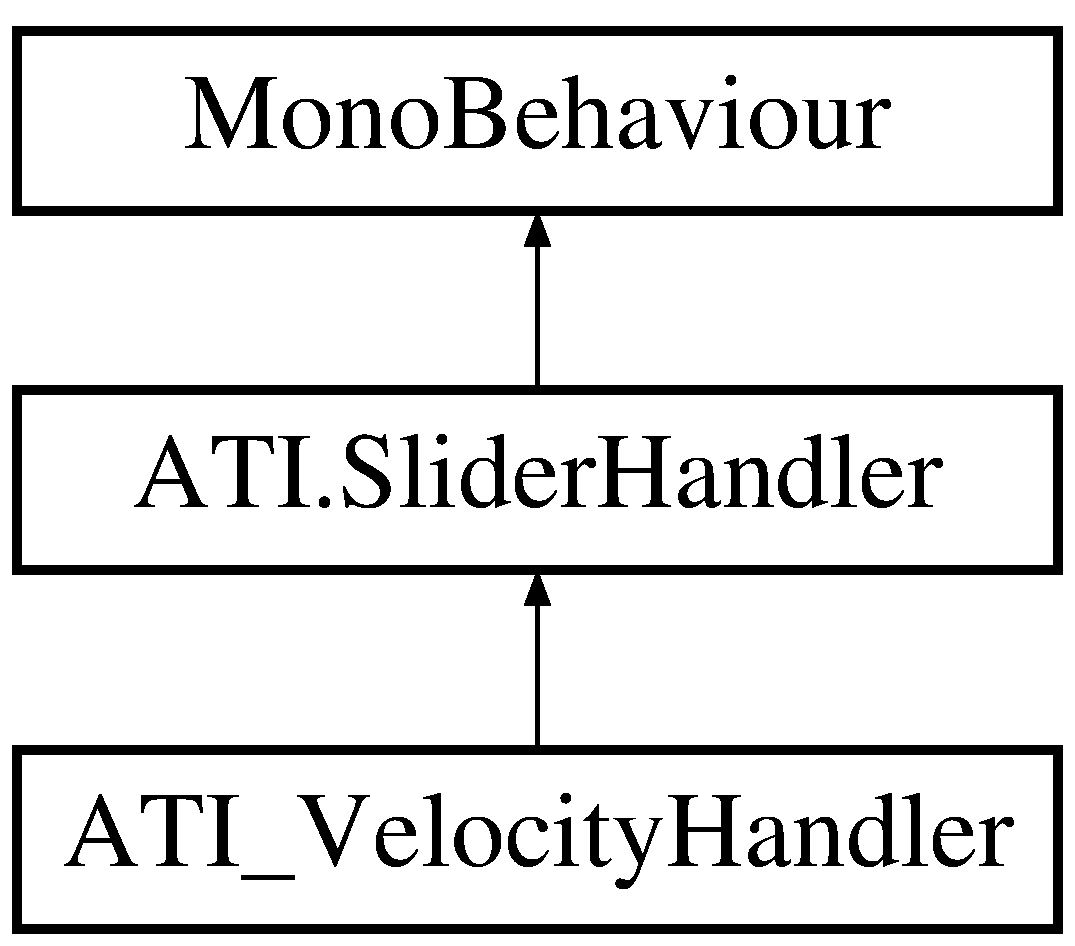
\includegraphics[height=3.000000cm]{class_a_t_i___velocity_handler}
\end{center}
\end{figure}
\subsection*{Public Member Functions}
\begin{DoxyCompactItemize}
\item 
void \hyperlink{class_a_t_i___velocity_handler_a1091248299687641294f363aa32de0f0}{On\+Randomize\+Velocity\+Switch} (bool a\+Switch)
\end{DoxyCompactItemize}
\subsection*{Protected Member Functions}
\begin{DoxyCompactItemize}
\item 
override void \hyperlink{class_a_t_i___velocity_handler_a6e1fd3ceb35873a09e138bebd0c323fd}{Handle\+Highest\+Random\+Velocity\+Change} (bool a\+End\+Drag)
\item 
override void \hyperlink{class_a_t_i___velocity_handler_a17b6e0de9e45dfb9dba1ea4f2c0a122c}{Handle\+Lowest\+Random\+Velocity\+Change} (bool a\+End\+Drag)
\item 
override void \hyperlink{class_a_t_i___velocity_handler_a5b00635239f4f10aaefc5898a8f1b975}{Handle\+Musical\+Typing\+Key\+Velocity\+Change} (int a\+Slider\+Index)
\end{DoxyCompactItemize}
\subsection*{Private Member Functions}
\begin{DoxyCompactItemize}
\item 
new void \hyperlink{class_a_t_i___velocity_handler_a76342d6f2b240a3007b20b9539e4c7a6}{Start} ()
\item 
void \hyperlink{class_a_t_i___velocity_handler_aa5766a74ea02f8e1d789a3863ce5867b}{Update} ()
\item 
void \hyperlink{class_a_t_i___velocity_handler_aa1a10281dafc6666677e4255ad663dde}{Randomize\+Key\+Velocities} ()
\end{DoxyCompactItemize}
\subsection*{Private Attributes}
\begin{DoxyCompactItemize}
\item 
string \mbox{[}$\,$\mbox{]} \hyperlink{class_a_t_i___velocity_handler_a95a1abb133981ac42dce424f0f94d562}{keys}
\item 
\hyperlink{class_a_t_i_1_1_slider_trigger}{A\+T\+I.\+Slider\+Trigger} \hyperlink{class_a_t_i___velocity_handler_aae4118883cf2e5489ef483f220e48e45}{m\+Highest\+Random\+Slider\+Trigger} = null
\item 
\hyperlink{class_a_t_i_1_1_slider_trigger}{A\+T\+I.\+Slider\+Trigger} \hyperlink{class_a_t_i___velocity_handler_a13d55e2f5670e3f1eb78645a75aa1bce}{m\+Lowest\+Random\+Slider\+Trigger} = null
\item 
bool \hyperlink{class_a_t_i___velocity_handler_aa6f4ac16382d37eb2c66fb358ac87301}{m\+Randomize} = false
\item 
Slider \hyperlink{class_a_t_i___velocity_handler_aba4ceb157ad404a47cedb3583e81d194}{m\+Lowest\+Random\+Slider} = null
\item 
Slider \hyperlink{class_a_t_i___velocity_handler_aec243511d869243292e215a24e87f192}{m\+Highest\+Random\+Slider} = null
\item 
Sprite \mbox{[}$\,$\mbox{]} \hyperlink{class_a_t_i___velocity_handler_a7e2452c41bbcdd313afb2e53fac4a975}{m\+Sprites} = null
\item 
Text \mbox{[}$\,$\mbox{]} \hyperlink{class_a_t_i___velocity_handler_ad8c048670a748ece6b2f8bbf287e7674}{m\+Text} = null
\item 
Toggle \hyperlink{class_a_t_i___velocity_handler_a6ca709a10f8b2eb0f1141c589e7f9742}{m\+Random\+Toggle} = null
\end{DoxyCompactItemize}
\subsection*{Additional Inherited Members}


\subsection{Detailed Description}


Definition at line 16 of file A\+T\+I\+\_\+\+Velocity\+Handler.\+cs.



\subsection{Member Function Documentation}
\mbox{\Hypertarget{class_a_t_i___velocity_handler_a6e1fd3ceb35873a09e138bebd0c323fd}\label{class_a_t_i___velocity_handler_a6e1fd3ceb35873a09e138bebd0c323fd}} 
\index{A\+T\+I\+\_\+\+Velocity\+Handler@{A\+T\+I\+\_\+\+Velocity\+Handler}!Handle\+Highest\+Random\+Velocity\+Change@{Handle\+Highest\+Random\+Velocity\+Change}}
\index{Handle\+Highest\+Random\+Velocity\+Change@{Handle\+Highest\+Random\+Velocity\+Change}!A\+T\+I\+\_\+\+Velocity\+Handler@{A\+T\+I\+\_\+\+Velocity\+Handler}}
\subsubsection{\texorpdfstring{Handle\+Highest\+Random\+Velocity\+Change()}{HandleHighestRandomVelocityChange()}}
{\footnotesize\ttfamily override void A\+T\+I\+\_\+\+Velocity\+Handler.\+Handle\+Highest\+Random\+Velocity\+Change (\begin{DoxyParamCaption}\item[{bool}]{a\+End\+Drag }\end{DoxyParamCaption})\hspace{0.3cm}{\ttfamily [protected]}, {\ttfamily [virtual]}}



Reimplemented from \hyperlink{class_a_t_i_1_1_slider_handler_a827fab40da8ee6e777cbed4b5a9ae712}{A\+T\+I.\+Slider\+Handler}.



Definition at line 124 of file A\+T\+I\+\_\+\+Velocity\+Handler.\+cs.



References Randomize\+Key\+Velocities().


\begin{DoxyCode}
125     \{
126         \textcolor{comment}{// Set the text and update the lowest random velocity slider's max value.}
127         \hyperlink{class_a_t_i___velocity_handler_aec243511d869243292e215a24e87f192}{mHighestRandomSlider}.transform.GetChild( 4 ).GetComponent<Text>().text = \textcolor{stringliteral}{"
      Highest: "} + \hyperlink{class_a_t_i___velocity_handler_aec243511d869243292e215a24e87f192}{mHighestRandomSlider}.value.ToString();
128         \hyperlink{class_a_t_i___velocity_handler_aba4ceb157ad404a47cedb3583e81d194}{mLowestRandomSlider}.maxValue = \hyperlink{class_a_t_i___velocity_handler_aec243511d869243292e215a24e87f192}{mHighestRandomSlider}.value;
129 
130         \textcolor{comment}{// If the value is set, then randomize the velocities for each key.}
131         \textcolor{keywordflow}{if}( aEndDrag && \hyperlink{class_a_t_i___velocity_handler_aa6f4ac16382d37eb2c66fb358ac87301}{mRandomize} )
132         \{
133             \hyperlink{class_a_t_i___velocity_handler_aa1a10281dafc6666677e4255ad663dde}{RandomizeKeyVelocities}();
134         \}
135     \}
\end{DoxyCode}
\mbox{\Hypertarget{class_a_t_i___velocity_handler_a17b6e0de9e45dfb9dba1ea4f2c0a122c}\label{class_a_t_i___velocity_handler_a17b6e0de9e45dfb9dba1ea4f2c0a122c}} 
\index{A\+T\+I\+\_\+\+Velocity\+Handler@{A\+T\+I\+\_\+\+Velocity\+Handler}!Handle\+Lowest\+Random\+Velocity\+Change@{Handle\+Lowest\+Random\+Velocity\+Change}}
\index{Handle\+Lowest\+Random\+Velocity\+Change@{Handle\+Lowest\+Random\+Velocity\+Change}!A\+T\+I\+\_\+\+Velocity\+Handler@{A\+T\+I\+\_\+\+Velocity\+Handler}}
\subsubsection{\texorpdfstring{Handle\+Lowest\+Random\+Velocity\+Change()}{HandleLowestRandomVelocityChange()}}
{\footnotesize\ttfamily override void A\+T\+I\+\_\+\+Velocity\+Handler.\+Handle\+Lowest\+Random\+Velocity\+Change (\begin{DoxyParamCaption}\item[{bool}]{a\+End\+Drag }\end{DoxyParamCaption})\hspace{0.3cm}{\ttfamily [protected]}, {\ttfamily [virtual]}}



Reimplemented from \hyperlink{class_a_t_i_1_1_slider_handler_a710b59b6e8bf059af76477a930572d9e}{A\+T\+I.\+Slider\+Handler}.



Definition at line 139 of file A\+T\+I\+\_\+\+Velocity\+Handler.\+cs.



References Randomize\+Key\+Velocities().


\begin{DoxyCode}
140     \{
141         \textcolor{comment}{// Set the text and update the highest random velocity slider's min value.}
142         \hyperlink{class_a_t_i___velocity_handler_aba4ceb157ad404a47cedb3583e81d194}{mLowestRandomSlider}.transform.GetChild( 4 ).GetComponent<Text>().text = \textcolor{stringliteral}{"Lowest:
       "} + \hyperlink{class_a_t_i___velocity_handler_aba4ceb157ad404a47cedb3583e81d194}{mLowestRandomSlider}.value.ToString();
143         \hyperlink{class_a_t_i___velocity_handler_aec243511d869243292e215a24e87f192}{mHighestRandomSlider}.minValue = \hyperlink{class_a_t_i___velocity_handler_aba4ceb157ad404a47cedb3583e81d194}{mLowestRandomSlider}.value;
144 
145         \textcolor{comment}{// If the value is set, then randomize the velocities for each key.}
146         \textcolor{keywordflow}{if}( aEndDrag && \hyperlink{class_a_t_i___velocity_handler_aa6f4ac16382d37eb2c66fb358ac87301}{mRandomize} )
147         \{
148             \hyperlink{class_a_t_i___velocity_handler_aa1a10281dafc6666677e4255ad663dde}{RandomizeKeyVelocities}();
149         \}
150     \}
\end{DoxyCode}
\mbox{\Hypertarget{class_a_t_i___velocity_handler_a5b00635239f4f10aaefc5898a8f1b975}\label{class_a_t_i___velocity_handler_a5b00635239f4f10aaefc5898a8f1b975}} 
\index{A\+T\+I\+\_\+\+Velocity\+Handler@{A\+T\+I\+\_\+\+Velocity\+Handler}!Handle\+Musical\+Typing\+Key\+Velocity\+Change@{Handle\+Musical\+Typing\+Key\+Velocity\+Change}}
\index{Handle\+Musical\+Typing\+Key\+Velocity\+Change@{Handle\+Musical\+Typing\+Key\+Velocity\+Change}!A\+T\+I\+\_\+\+Velocity\+Handler@{A\+T\+I\+\_\+\+Velocity\+Handler}}
\subsubsection{\texorpdfstring{Handle\+Musical\+Typing\+Key\+Velocity\+Change()}{HandleMusicalTypingKeyVelocityChange()}}
{\footnotesize\ttfamily override void A\+T\+I\+\_\+\+Velocity\+Handler.\+Handle\+Musical\+Typing\+Key\+Velocity\+Change (\begin{DoxyParamCaption}\item[{int}]{a\+Slider\+Index }\end{DoxyParamCaption})\hspace{0.3cm}{\ttfamily [protected]}, {\ttfamily [virtual]}}



Reimplemented from \hyperlink{class_a_t_i_1_1_slider_handler_ac82219a0a69f17025d9484f9e45cca80}{A\+T\+I.\+Slider\+Handler}.



Definition at line 154 of file A\+T\+I\+\_\+\+Velocity\+Handler.\+cs.



References Virtual\+Instrument\+Manager.\+Get\+Musical\+Typing\+Handler(), A\+T\+I.\+Slider\+Handler.\+m\+Sliders, A\+T\+I.\+Slider\+Handler.\+m\+V\+IM, and Musical\+Typing\+Handler.\+Set\+Key\+Velocity().


\begin{DoxyCode}
155     \{
156         \textcolor{comment}{// Change the text and pass the value to the virtual instrument manager.}
157         \hyperlink{class_a_t_i___velocity_handler_ad8c048670a748ece6b2f8bbf287e7674}{mText}[aSliderIndex].text = \hyperlink{class_a_t_i___velocity_handler_a95a1abb133981ac42dce424f0f94d562}{keys}[aSliderIndex] + \hyperlink{class_a_t_i_1_1_slider_handler_a038a487fbd701cb786e77c210830be76}{mSliders}[aSliderIndex].value.
      ToString();
158         \hyperlink{class_a_t_i_1_1_slider_handler_a5d19b4fb92b71c25a667defdda60213f}{mVIM}.\hyperlink{group___v_i_m_pub_func_gae6701458a23a3f14db90501f871d4d0d}{GetMusicalTypingHandler}().\hyperlink{group___mus_typ_pub_func_ga02f86b46bb63dc751b669035b7aa5ce0}{SetKeyVelocity}( 
      aSliderIndex, (\textcolor{keywordtype}{int})\hyperlink{class_a_t_i_1_1_slider_handler_a038a487fbd701cb786e77c210830be76}{mSliders}[aSliderIndex].value );
159     \}
\end{DoxyCode}
\mbox{\Hypertarget{class_a_t_i___velocity_handler_a1091248299687641294f363aa32de0f0}\label{class_a_t_i___velocity_handler_a1091248299687641294f363aa32de0f0}} 
\index{A\+T\+I\+\_\+\+Velocity\+Handler@{A\+T\+I\+\_\+\+Velocity\+Handler}!On\+Randomize\+Velocity\+Switch@{On\+Randomize\+Velocity\+Switch}}
\index{On\+Randomize\+Velocity\+Switch@{On\+Randomize\+Velocity\+Switch}!A\+T\+I\+\_\+\+Velocity\+Handler@{A\+T\+I\+\_\+\+Velocity\+Handler}}
\subsubsection{\texorpdfstring{On\+Randomize\+Velocity\+Switch()}{OnRandomizeVelocitySwitch()}}
{\footnotesize\ttfamily void A\+T\+I\+\_\+\+Velocity\+Handler.\+On\+Randomize\+Velocity\+Switch (\begin{DoxyParamCaption}\item[{bool}]{a\+Switch }\end{DoxyParamCaption})}



Definition at line 163 of file A\+T\+I\+\_\+\+Velocity\+Handler.\+cs.



References Randomize\+Key\+Velocities().



Referenced by Start().


\begin{DoxyCode}
164     \{
165         \textcolor{keywordflow}{if}( aSwitch )
166         \{
167             \textcolor{comment}{// If the switch has been turned on, update the image and text and randomize the musical typing}
168             \textcolor{comment}{// key velocities.}
169             \hyperlink{class_a_t_i___velocity_handler_aa6f4ac16382d37eb2c66fb358ac87301}{mRandomize} = \textcolor{keyword}{true};
170             \hyperlink{class_a_t_i___velocity_handler_a6ca709a10f8b2eb0f1141c589e7f9742}{mRandomToggle}.transform.GetChild( 1 ).GetComponent<Image>().sprite = 
      \hyperlink{class_a_t_i___velocity_handler_a7e2452c41bbcdd313afb2e53fac4a975}{mSprites}[1];
171             \hyperlink{class_a_t_i___velocity_handler_a6ca709a10f8b2eb0f1141c589e7f9742}{mRandomToggle}.transform.GetChild( 2 ).GetComponent<Text>().text = \textcolor{stringliteral}{"Randomize
       Velocities:\(\backslash\)nOn"};
172             \hyperlink{class_a_t_i___velocity_handler_aa1a10281dafc6666677e4255ad663dde}{RandomizeKeyVelocities}();
173         \}
174         \textcolor{keywordflow}{else}
175         \{
176             \textcolor{comment}{// If the switch has been turned off, then update the image and the text.}
177             \hyperlink{class_a_t_i___velocity_handler_a6ca709a10f8b2eb0f1141c589e7f9742}{mRandomToggle}.transform.GetChild( 1 ).GetComponent<Image>().sprite = 
      \hyperlink{class_a_t_i___velocity_handler_a7e2452c41bbcdd313afb2e53fac4a975}{mSprites}[0];
178             \hyperlink{class_a_t_i___velocity_handler_a6ca709a10f8b2eb0f1141c589e7f9742}{mRandomToggle}.transform.GetChild( 2 ).GetComponent<Text>().text = \textcolor{stringliteral}{"Randomize
       Velocities:\(\backslash\)nOff"};
179             \hyperlink{class_a_t_i___velocity_handler_aa6f4ac16382d37eb2c66fb358ac87301}{mRandomize} = \textcolor{keyword}{false};
180         \}
181     \}
\end{DoxyCode}
\mbox{\Hypertarget{class_a_t_i___velocity_handler_aa1a10281dafc6666677e4255ad663dde}\label{class_a_t_i___velocity_handler_aa1a10281dafc6666677e4255ad663dde}} 
\index{A\+T\+I\+\_\+\+Velocity\+Handler@{A\+T\+I\+\_\+\+Velocity\+Handler}!Randomize\+Key\+Velocities@{Randomize\+Key\+Velocities}}
\index{Randomize\+Key\+Velocities@{Randomize\+Key\+Velocities}!A\+T\+I\+\_\+\+Velocity\+Handler@{A\+T\+I\+\_\+\+Velocity\+Handler}}
\subsubsection{\texorpdfstring{Randomize\+Key\+Velocities()}{RandomizeKeyVelocities()}}
{\footnotesize\ttfamily void A\+T\+I\+\_\+\+Velocity\+Handler.\+Randomize\+Key\+Velocities (\begin{DoxyParamCaption}{ }\end{DoxyParamCaption})\hspace{0.3cm}{\ttfamily [private]}}



Definition at line 111 of file A\+T\+I\+\_\+\+Velocity\+Handler.\+cs.



References Virtual\+Instrument\+Manager.\+Get\+Musical\+Typing\+Handler(), m\+Randomize, A\+T\+I.\+Slider\+Handler.\+m\+V\+IM, Musical\+Typing\+Handler.\+Randomize\+Velocities, and Musical\+Typing\+Handler.\+Set\+Random\+Velocity\+Range().



Referenced by Handle\+Highest\+Random\+Velocity\+Change(), Handle\+Lowest\+Random\+Velocity\+Change(), and On\+Randomize\+Velocity\+Switch().


\begin{DoxyCode}
112     \{
113         \hyperlink{class_a_t_i___velocity_handler_aa6f4ac16382d37eb2c66fb358ac87301}{mRandomize} = \hyperlink{class_a_t_i___velocity_handler_a6ca709a10f8b2eb0f1141c589e7f9742}{mRandomToggle}.enabled;
114         \hyperlink{class_a_t_i_1_1_slider_handler_a5d19b4fb92b71c25a667defdda60213f}{mVIM}.\hyperlink{group___v_i_m_pub_func_gae6701458a23a3f14db90501f871d4d0d}{GetMusicalTypingHandler}().
      \hyperlink{group___mus_typ_pub_var_gad09f6f673034d9cd95f699838c9518d5}{RandomizeVelocities} = \hyperlink{class_a_t_i___velocity_handler_aa6f4ac16382d37eb2c66fb358ac87301}{mRandomize};
115         \hyperlink{class_a_t_i_1_1_slider_handler_a5d19b4fb92b71c25a667defdda60213f}{mVIM}.\hyperlink{group___v_i_m_pub_func_gae6701458a23a3f14db90501f871d4d0d}{GetMusicalTypingHandler}().
      \hyperlink{group___mus_typ_pub_func_gaf6ba35e3a081cff62fa963ed32d218c8}{SetRandomVelocityRange}( (\textcolor{keywordtype}{int})\hyperlink{class_a_t_i___velocity_handler_aba4ceb157ad404a47cedb3583e81d194}{mLowestRandomSlider}.value, (\textcolor{keywordtype}{int})
      \hyperlink{class_a_t_i___velocity_handler_aec243511d869243292e215a24e87f192}{mHighestRandomSlider}.value );
116     \}
\end{DoxyCode}
\mbox{\Hypertarget{class_a_t_i___velocity_handler_a76342d6f2b240a3007b20b9539e4c7a6}\label{class_a_t_i___velocity_handler_a76342d6f2b240a3007b20b9539e4c7a6}} 
\index{A\+T\+I\+\_\+\+Velocity\+Handler@{A\+T\+I\+\_\+\+Velocity\+Handler}!Start@{Start}}
\index{Start@{Start}!A\+T\+I\+\_\+\+Velocity\+Handler@{A\+T\+I\+\_\+\+Velocity\+Handler}}
\subsubsection{\texorpdfstring{Start()}{Start()}}
{\footnotesize\ttfamily new void A\+T\+I\+\_\+\+Velocity\+Handler.\+Start (\begin{DoxyParamCaption}{ }\end{DoxyParamCaption})\hspace{0.3cm}{\ttfamily [private]}}



Definition at line 46 of file A\+T\+I\+\_\+\+Velocity\+Handler.\+cs.



References m\+Highest\+Random\+Slider\+Trigger, m\+Lowest\+Random\+Slider\+Trigger, A\+T\+I.\+Slider\+Handler.\+m\+Num\+Sliders, A\+T\+I.\+Slider\+Handler.\+m\+Sliders, A\+T\+I.\+Slider\+Handler.\+m\+Slider\+Triggers, On\+Randomize\+Velocity\+Switch(), A\+T\+I.\+Slider\+Trigger.\+Set\+Handler(), and A\+T\+I.\+Slider\+Trigger.\+Set\+Type().


\begin{DoxyCode}
47     \{
48 
49 \textcolor{preprocessor}{#if DEBUG && DEBUG\_MUSICAL\_TYPING}
50 
51         \textcolor{comment}{// Call the ATI.SliderHandler start function.}
52         base.Start();
53 
54         \textcolor{comment}{// Set the images for the randomize musical typing velocities switch.}
55         \hyperlink{class_a_t_i___velocity_handler_a7e2452c41bbcdd313afb2e53fac4a975}{mSprites} = \textcolor{keyword}{new} Sprite[2];
56         \hyperlink{class_a_t_i___velocity_handler_a7e2452c41bbcdd313afb2e53fac4a975}{mSprites}[0] = Resources.Load<Sprite>( \textcolor{stringliteral}{"Audio/Images/off\_button"} );
57         \hyperlink{class_a_t_i___velocity_handler_a7e2452c41bbcdd313afb2e53fac4a975}{mSprites}[1] = Resources.Load<Sprite>( \textcolor{stringliteral}{"Audio/Images/on\_button"} );
58 
59         \textcolor{comment}{// Set the toggle switch for randomizing musical typing velocities}
60         \hyperlink{class_a_t_i___velocity_handler_a6ca709a10f8b2eb0f1141c589e7f9742}{mRandomToggle} = gameObject.transform.GetChild( 0 ).GetComponent<Toggle>();
61         mRandomToggle.onValueChanged.AddListener( \hyperlink{class_a_t_i___velocity_handler_a1091248299687641294f363aa32de0f0}{OnRandomizeVelocitySwitch} );
62 
63         \textcolor{comment}{// Set the lowest random value slider.}
64         \hyperlink{class_a_t_i___velocity_handler_aba4ceb157ad404a47cedb3583e81d194}{mLowestRandomSlider} = gameObject.transform.GetChild( 1 ).GetComponent<Slider>();
65         \hyperlink{class_a_t_i___velocity_handler_a13d55e2f5670e3f1eb78645a75aa1bce}{mLowestRandomSliderTrigger} = 
      \hyperlink{class_a_t_i___velocity_handler_aba4ceb157ad404a47cedb3583e81d194}{mLowestRandomSlider}.gameObject.AddComponent<\hyperlink{class_a_t_i}{ATI}.
      \hyperlink{class_a_t_i_1_1_slider_trigger}{SliderTrigger}>();
66         mLowestRandomSliderTrigger.\hyperlink{class_a_t_i_1_1_slider_trigger_a258f79d013266d0c82a5382525adcdef}{SetHandler}( \textcolor{keyword}{this} );
67         mLowestRandomSliderTrigger.SetType( \hyperlink{class_a_t_i}{ATI}.\hyperlink{class_a_t_i_ac4c6056a99cbd16ff0d292d33b038b9b}{SliderType}.LowestRandomKeyVelocity );
68 
69         \textcolor{comment}{// Set the highest random value slider.}
70         \hyperlink{class_a_t_i___velocity_handler_aec243511d869243292e215a24e87f192}{mHighestRandomSlider} = gameObject.transform.GetChild( 2 ).GetComponent<Slider>(
      );
71         \hyperlink{class_a_t_i___velocity_handler_aae4118883cf2e5489ef483f220e48e45}{mHighestRandomSliderTrigger} = 
      \hyperlink{class_a_t_i___velocity_handler_aec243511d869243292e215a24e87f192}{mHighestRandomSlider}.gameObject.AddComponent<\hyperlink{class_a_t_i}{ATI}.
      \hyperlink{class_a_t_i_1_1_slider_trigger}{SliderTrigger}>();
72         mHighestRandomSliderTrigger.\hyperlink{class_a_t_i_1_1_slider_trigger_a258f79d013266d0c82a5382525adcdef}{SetHandler}( \textcolor{keyword}{this} );
73         mHighestRandomSliderTrigger.SetType( \hyperlink{class_a_t_i}{ATI}.\hyperlink{class_a_t_i_ac4c6056a99cbd16ff0d292d33b038b9b}{SliderType}.HighestRandomKeyVelocity );
74 
75         \textcolor{comment}{// Initialize the sliders, their text, and their triggers.}
76         \hyperlink{class_a_t_i_1_1_slider_handler_ac762fad2fb523da79188668dde4488ec}{mNumSliders} = 19;
77         \hyperlink{class_a_t_i_1_1_slider_handler_a038a487fbd701cb786e77c210830be76}{mSliders} = \textcolor{keyword}{new} Slider[\hyperlink{class_a_t_i_1_1_slider_handler_ac762fad2fb523da79188668dde4488ec}{mNumSliders}];
78         \hyperlink{class_a_t_i___velocity_handler_ad8c048670a748ece6b2f8bbf287e7674}{mText} = \textcolor{keyword}{new} Text[\hyperlink{class_a_t_i_1_1_slider_handler_ac762fad2fb523da79188668dde4488ec}{mNumSliders}];
79         \hyperlink{class_a_t_i_1_1_slider_handler_a20208bc52a906cf87aa9df8e5fb2c636}{mSliderTriggers} = \textcolor{keyword}{new} \hyperlink{class_a_t_i}{ATI}.\hyperlink{class_a_t_i_1_1_slider_trigger}{SliderTrigger}[
      \hyperlink{class_a_t_i_1_1_slider_handler_ac762fad2fb523da79188668dde4488ec}{mNumSliders}];
80 
81         \textcolor{keywordflow}{for}( \textcolor{keywordtype}{int} i = 0; i < \hyperlink{class_a_t_i_1_1_slider_handler_ac762fad2fb523da79188668dde4488ec}{mNumSliders}; i++ )
82         \{
83             \textcolor{comment}{// For each slider, put it in the array and add the slider trigger.}
84             \hyperlink{class_a_t_i_1_1_slider_handler_a038a487fbd701cb786e77c210830be76}{mSliders}[i] = gameObject.transform.GetChild( i + 3 ).GetComponent<Slider>();
85             \hyperlink{class_a_t_i_1_1_slider_handler_a20208bc52a906cf87aa9df8e5fb2c636}{mSliderTriggers}[i] = \hyperlink{class_a_t_i_1_1_slider_handler_a038a487fbd701cb786e77c210830be76}{mSliders}[i].gameObject.AddComponent<
      \hyperlink{class_a_t_i}{ATI}.\hyperlink{class_a_t_i_1_1_slider_trigger}{SliderTrigger}>();
86             mSliderTriggers[i].\hyperlink{class_a_t_i_1_1_slider_trigger_a90347192aede3444d468ed2ab0d97f6c}{SetType}( \hyperlink{class_a_t_i}{ATI}.\hyperlink{class_a_t_i_ac4c6056a99cbd16ff0d292d33b038b9b}{SliderType}.MusicalTypingKeyVelocity );
87             mSliderTriggers[i].SetHandler( \textcolor{keyword}{this} );
88 
89             \textcolor{comment}{// For each text, put it in the array and set its value}
90             \hyperlink{class_a_t_i___velocity_handler_ad8c048670a748ece6b2f8bbf287e7674}{mText}[i] = \hyperlink{class_a_t_i_1_1_slider_handler_a038a487fbd701cb786e77c210830be76}{mSliders}[i].gameObject.transform.GetChild( 4 ).GetComponent<Text>();
91             \hyperlink{class_a_t_i___velocity_handler_ad8c048670a748ece6b2f8bbf287e7674}{mText}[i].text = \hyperlink{class_a_t_i___velocity_handler_a95a1abb133981ac42dce424f0f94d562}{keys}[i] + \textcolor{stringliteral}{"100"};
92         \}
93 \textcolor{preprocessor}{#endif}
94 
95     \}
\end{DoxyCode}
\mbox{\Hypertarget{class_a_t_i___velocity_handler_aa5766a74ea02f8e1d789a3863ce5867b}\label{class_a_t_i___velocity_handler_aa5766a74ea02f8e1d789a3863ce5867b}} 
\index{A\+T\+I\+\_\+\+Velocity\+Handler@{A\+T\+I\+\_\+\+Velocity\+Handler}!Update@{Update}}
\index{Update@{Update}!A\+T\+I\+\_\+\+Velocity\+Handler@{A\+T\+I\+\_\+\+Velocity\+Handler}}
\subsubsection{\texorpdfstring{Update()}{Update()}}
{\footnotesize\ttfamily void A\+T\+I\+\_\+\+Velocity\+Handler.\+Update (\begin{DoxyParamCaption}{ }\end{DoxyParamCaption})\hspace{0.3cm}{\ttfamily [private]}}



Definition at line 99 of file A\+T\+I\+\_\+\+Velocity\+Handler.\+cs.


\begin{DoxyCode}
100     \{
101 
102     \}
\end{DoxyCode}


\subsection{Member Data Documentation}
\mbox{\Hypertarget{class_a_t_i___velocity_handler_a95a1abb133981ac42dce424f0f94d562}\label{class_a_t_i___velocity_handler_a95a1abb133981ac42dce424f0f94d562}} 
\index{A\+T\+I\+\_\+\+Velocity\+Handler@{A\+T\+I\+\_\+\+Velocity\+Handler}!keys@{keys}}
\index{keys@{keys}!A\+T\+I\+\_\+\+Velocity\+Handler@{A\+T\+I\+\_\+\+Velocity\+Handler}}
\subsubsection{\texorpdfstring{keys}{keys}}
{\footnotesize\ttfamily string \mbox{[}$\,$\mbox{]} A\+T\+I\+\_\+\+Velocity\+Handler.\+keys\hspace{0.3cm}{\ttfamily [private]}}

{\bfseries Initial value\+:}
\begin{DoxyCode}
=
        \{ \textcolor{stringliteral}{"a: "}, \textcolor{stringliteral}{"w: "}, \textcolor{stringliteral}{"s: "}, \textcolor{stringliteral}{"e: "}, \textcolor{stringliteral}{"d: "}, \textcolor{stringliteral}{"f: "}, \textcolor{stringliteral}{"t: "}, \textcolor{stringliteral}{"g: "}, \textcolor{stringliteral}{"y: "}, \textcolor{stringliteral}{"h: "}, \textcolor{stringliteral}{"u: "}, \textcolor{stringliteral}{"j: "}, \textcolor{stringliteral}{"k: "}, \textcolor{stringliteral}{"o: "},
       \textcolor{stringliteral}{"l: "}, \textcolor{stringliteral}{"p: "}, \textcolor{stringliteral}{";: "}, \textcolor{stringliteral}{"': "}, \textcolor{stringliteral}{"]: "} \}
\end{DoxyCode}


Definition at line 24 of file A\+T\+I\+\_\+\+Velocity\+Handler.\+cs.

\mbox{\Hypertarget{class_a_t_i___velocity_handler_aec243511d869243292e215a24e87f192}\label{class_a_t_i___velocity_handler_aec243511d869243292e215a24e87f192}} 
\index{A\+T\+I\+\_\+\+Velocity\+Handler@{A\+T\+I\+\_\+\+Velocity\+Handler}!m\+Highest\+Random\+Slider@{m\+Highest\+Random\+Slider}}
\index{m\+Highest\+Random\+Slider@{m\+Highest\+Random\+Slider}!A\+T\+I\+\_\+\+Velocity\+Handler@{A\+T\+I\+\_\+\+Velocity\+Handler}}
\subsubsection{\texorpdfstring{m\+Highest\+Random\+Slider}{mHighestRandomSlider}}
{\footnotesize\ttfamily Slider A\+T\+I\+\_\+\+Velocity\+Handler.\+m\+Highest\+Random\+Slider = null\hspace{0.3cm}{\ttfamily [private]}}



Definition at line 34 of file A\+T\+I\+\_\+\+Velocity\+Handler.\+cs.

\mbox{\Hypertarget{class_a_t_i___velocity_handler_aae4118883cf2e5489ef483f220e48e45}\label{class_a_t_i___velocity_handler_aae4118883cf2e5489ef483f220e48e45}} 
\index{A\+T\+I\+\_\+\+Velocity\+Handler@{A\+T\+I\+\_\+\+Velocity\+Handler}!m\+Highest\+Random\+Slider\+Trigger@{m\+Highest\+Random\+Slider\+Trigger}}
\index{m\+Highest\+Random\+Slider\+Trigger@{m\+Highest\+Random\+Slider\+Trigger}!A\+T\+I\+\_\+\+Velocity\+Handler@{A\+T\+I\+\_\+\+Velocity\+Handler}}
\subsubsection{\texorpdfstring{m\+Highest\+Random\+Slider\+Trigger}{mHighestRandomSliderTrigger}}
{\footnotesize\ttfamily \hyperlink{class_a_t_i_1_1_slider_trigger}{A\+T\+I.\+Slider\+Trigger} A\+T\+I\+\_\+\+Velocity\+Handler.\+m\+Highest\+Random\+Slider\+Trigger = null\hspace{0.3cm}{\ttfamily [private]}}



Definition at line 30 of file A\+T\+I\+\_\+\+Velocity\+Handler.\+cs.



Referenced by Start().

\mbox{\Hypertarget{class_a_t_i___velocity_handler_aba4ceb157ad404a47cedb3583e81d194}\label{class_a_t_i___velocity_handler_aba4ceb157ad404a47cedb3583e81d194}} 
\index{A\+T\+I\+\_\+\+Velocity\+Handler@{A\+T\+I\+\_\+\+Velocity\+Handler}!m\+Lowest\+Random\+Slider@{m\+Lowest\+Random\+Slider}}
\index{m\+Lowest\+Random\+Slider@{m\+Lowest\+Random\+Slider}!A\+T\+I\+\_\+\+Velocity\+Handler@{A\+T\+I\+\_\+\+Velocity\+Handler}}
\subsubsection{\texorpdfstring{m\+Lowest\+Random\+Slider}{mLowestRandomSlider}}
{\footnotesize\ttfamily Slider A\+T\+I\+\_\+\+Velocity\+Handler.\+m\+Lowest\+Random\+Slider = null\hspace{0.3cm}{\ttfamily [private]}}



Definition at line 33 of file A\+T\+I\+\_\+\+Velocity\+Handler.\+cs.

\mbox{\Hypertarget{class_a_t_i___velocity_handler_a13d55e2f5670e3f1eb78645a75aa1bce}\label{class_a_t_i___velocity_handler_a13d55e2f5670e3f1eb78645a75aa1bce}} 
\index{A\+T\+I\+\_\+\+Velocity\+Handler@{A\+T\+I\+\_\+\+Velocity\+Handler}!m\+Lowest\+Random\+Slider\+Trigger@{m\+Lowest\+Random\+Slider\+Trigger}}
\index{m\+Lowest\+Random\+Slider\+Trigger@{m\+Lowest\+Random\+Slider\+Trigger}!A\+T\+I\+\_\+\+Velocity\+Handler@{A\+T\+I\+\_\+\+Velocity\+Handler}}
\subsubsection{\texorpdfstring{m\+Lowest\+Random\+Slider\+Trigger}{mLowestRandomSliderTrigger}}
{\footnotesize\ttfamily \hyperlink{class_a_t_i_1_1_slider_trigger}{A\+T\+I.\+Slider\+Trigger} A\+T\+I\+\_\+\+Velocity\+Handler.\+m\+Lowest\+Random\+Slider\+Trigger = null\hspace{0.3cm}{\ttfamily [private]}}



Definition at line 31 of file A\+T\+I\+\_\+\+Velocity\+Handler.\+cs.



Referenced by Start().

\mbox{\Hypertarget{class_a_t_i___velocity_handler_aa6f4ac16382d37eb2c66fb358ac87301}\label{class_a_t_i___velocity_handler_aa6f4ac16382d37eb2c66fb358ac87301}} 
\index{A\+T\+I\+\_\+\+Velocity\+Handler@{A\+T\+I\+\_\+\+Velocity\+Handler}!m\+Randomize@{m\+Randomize}}
\index{m\+Randomize@{m\+Randomize}!A\+T\+I\+\_\+\+Velocity\+Handler@{A\+T\+I\+\_\+\+Velocity\+Handler}}
\subsubsection{\texorpdfstring{m\+Randomize}{mRandomize}}
{\footnotesize\ttfamily bool A\+T\+I\+\_\+\+Velocity\+Handler.\+m\+Randomize = false\hspace{0.3cm}{\ttfamily [private]}}



Definition at line 32 of file A\+T\+I\+\_\+\+Velocity\+Handler.\+cs.



Referenced by Randomize\+Key\+Velocities().

\mbox{\Hypertarget{class_a_t_i___velocity_handler_a6ca709a10f8b2eb0f1141c589e7f9742}\label{class_a_t_i___velocity_handler_a6ca709a10f8b2eb0f1141c589e7f9742}} 
\index{A\+T\+I\+\_\+\+Velocity\+Handler@{A\+T\+I\+\_\+\+Velocity\+Handler}!m\+Random\+Toggle@{m\+Random\+Toggle}}
\index{m\+Random\+Toggle@{m\+Random\+Toggle}!A\+T\+I\+\_\+\+Velocity\+Handler@{A\+T\+I\+\_\+\+Velocity\+Handler}}
\subsubsection{\texorpdfstring{m\+Random\+Toggle}{mRandomToggle}}
{\footnotesize\ttfamily Toggle A\+T\+I\+\_\+\+Velocity\+Handler.\+m\+Random\+Toggle = null\hspace{0.3cm}{\ttfamily [private]}}



Definition at line 37 of file A\+T\+I\+\_\+\+Velocity\+Handler.\+cs.

\mbox{\Hypertarget{class_a_t_i___velocity_handler_a7e2452c41bbcdd313afb2e53fac4a975}\label{class_a_t_i___velocity_handler_a7e2452c41bbcdd313afb2e53fac4a975}} 
\index{A\+T\+I\+\_\+\+Velocity\+Handler@{A\+T\+I\+\_\+\+Velocity\+Handler}!m\+Sprites@{m\+Sprites}}
\index{m\+Sprites@{m\+Sprites}!A\+T\+I\+\_\+\+Velocity\+Handler@{A\+T\+I\+\_\+\+Velocity\+Handler}}
\subsubsection{\texorpdfstring{m\+Sprites}{mSprites}}
{\footnotesize\ttfamily Sprite \mbox{[}$\,$\mbox{]} A\+T\+I\+\_\+\+Velocity\+Handler.\+m\+Sprites = null\hspace{0.3cm}{\ttfamily [private]}}



Definition at line 35 of file A\+T\+I\+\_\+\+Velocity\+Handler.\+cs.

\mbox{\Hypertarget{class_a_t_i___velocity_handler_ad8c048670a748ece6b2f8bbf287e7674}\label{class_a_t_i___velocity_handler_ad8c048670a748ece6b2f8bbf287e7674}} 
\index{A\+T\+I\+\_\+\+Velocity\+Handler@{A\+T\+I\+\_\+\+Velocity\+Handler}!m\+Text@{m\+Text}}
\index{m\+Text@{m\+Text}!A\+T\+I\+\_\+\+Velocity\+Handler@{A\+T\+I\+\_\+\+Velocity\+Handler}}
\subsubsection{\texorpdfstring{m\+Text}{mText}}
{\footnotesize\ttfamily Text \mbox{[}$\,$\mbox{]} A\+T\+I\+\_\+\+Velocity\+Handler.\+m\+Text = null\hspace{0.3cm}{\ttfamily [private]}}



Definition at line 36 of file A\+T\+I\+\_\+\+Velocity\+Handler.\+cs.



The documentation for this class was generated from the following file\+:\begin{DoxyCompactItemize}
\item 
D\+:/\+Documents/\+School Documents/2017\+Spring/\+E\+E\+C\+S542/\+V\+R\+Piano\+Project/\+Assets/\+Scripts/\+Audio/\+Testing/\hyperlink{_a_t_i___velocity_handler_8cs}{A\+T\+I\+\_\+\+Velocity\+Handler.\+cs}\end{DoxyCompactItemize}

\hypertarget{class_black_key}{}\section{Black\+Key Class Reference}
\label{class_black_key}\index{Black\+Key@{Black\+Key}}


A script for handling the behavior of a black key on the keyboard.  


Inheritance diagram for Black\+Key\+:\begin{figure}[H]
\begin{center}
\leavevmode
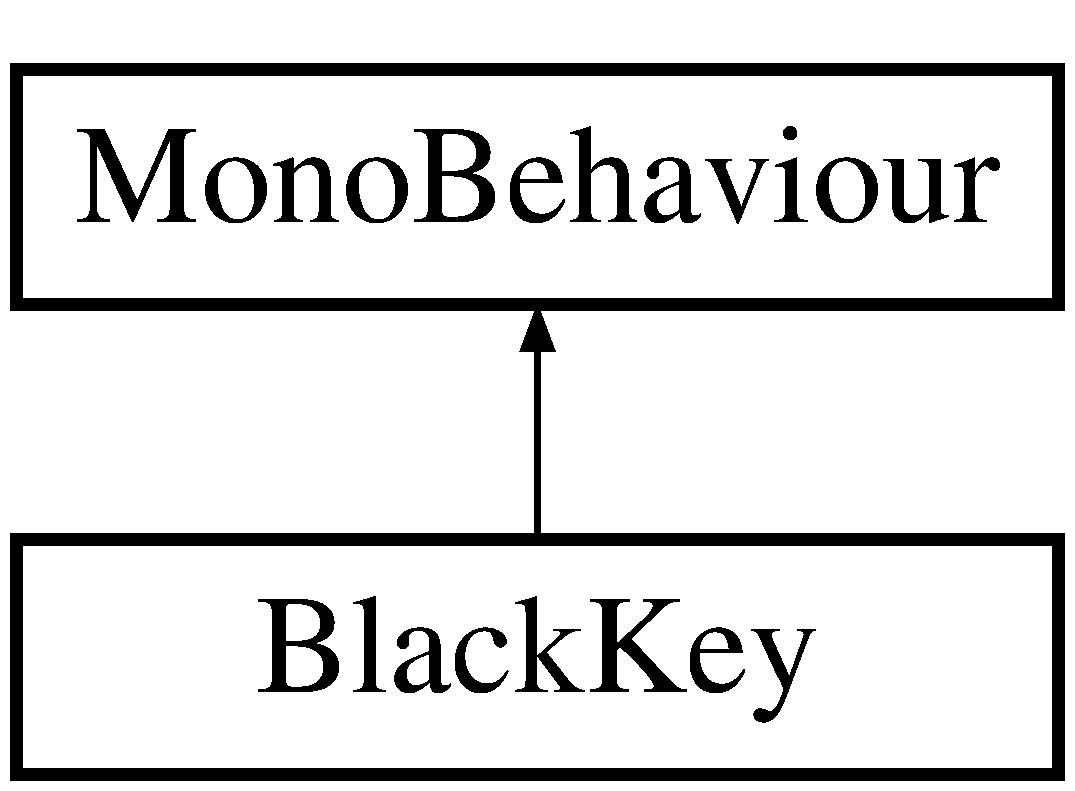
\includegraphics[height=2.000000cm]{class_black_key}
\end{center}
\end{figure}
\subsection*{Classes}
\begin{DoxyCompactItemize}
\item 
class \hyperlink{group___black_key_event_types_class_black_key_1_1_black_key_pressed_event}{Black\+Key\+Pressed\+Event}
\item 
class \hyperlink{group___black_key_event_types_class_black_key_1_1_black_key_released_event}{Black\+Key\+Released\+Event}
\begin{DoxyCompactList}\small\item\em $<$ Used for testing the container. Will probably need to change later.  \hyperlink{group___black_key_event_types_class_black_key_1_1_black_key_released_event}{More...}\end{DoxyCompactList}\end{DoxyCompactItemize}
\subsection*{Public Member Functions}
\begin{DoxyCompactItemize}
\item 
void \hyperlink{group___black_key_pub_func_ga49d807a46e36ba19211be329db1cbd2e}{Set\+Parent\+Container} (\hyperlink{class_key_container}{Key\+Container} a\+Container)
\begin{DoxyCompactList}\small\item\em Sets the \hyperlink{group___doc_key_contain}{parent container}. \end{DoxyCompactList}\end{DoxyCompactItemize}
\subsection*{Public Attributes}
\begin{DoxyCompactItemize}
\item 
\hyperlink{group___black_key_event_types_class_black_key_1_1_black_key_pressed_event}{Black\+Key\+Pressed\+Event} \hyperlink{group___black_key_events_ga51f1badf49df0c54e31a20ba4b7abd6b}{Black\+Key\+Pressed} = null
\begin{DoxyCompactList}\small\item\em Used for testing the container. Will probably need to change later. \end{DoxyCompactList}\item 
\hyperlink{group___black_key_event_types_class_black_key_1_1_black_key_released_event}{Black\+Key\+Released\+Event} \hyperlink{group___black_key_events_ga2710bdaba16dbdb82c0d38f11ce642d8}{Black\+Key\+Released} = null
\begin{DoxyCompactList}\small\item\em Used for testing the container. Will probably need to change later. \end{DoxyCompactList}\item 
float \hyperlink{group___black_key_pub_var_ga6fb983b09b3b6f80eab375fcb43010c1}{Velocity}
\begin{DoxyCompactList}\small\item\em The velocity of the key object. \end{DoxyCompactList}\item 
\hyperlink{group___music_enums_ga508f69b199ea518f935486c990edac1d}{Music.\+P\+I\+T\+CH} \hyperlink{group___black_key_pub_var_gad233c456182c9cef7c01486484940439}{Pitch} = \hyperlink{group___music_enums_gga508f69b199ea518f935486c990edac1da7009daf81333670cd06b8bb2b02054cc}{Music.\+P\+I\+T\+C\+H.\+C\+S4}
\begin{DoxyCompactList}\small\item\em The pitch that this key represents. \end{DoxyCompactList}\item 
string \hyperlink{group___black_key_pub_var_gaa541d3fb6cbb1361d5c062ce7b3c4e29}{Key} = \char`\"{}A\char`\"{}
\begin{DoxyCompactList}\small\item\em The key that begins pressing the black key. \end{DoxyCompactList}\end{DoxyCompactItemize}
\subsection*{Private Member Functions}
\begin{DoxyCompactItemize}
\item 
void \hyperlink{group___black_key_unity_ga6e05fcdf362e52d9a71b4f25ad840b5b}{Awake} ()
\begin{DoxyCompactList}\small\item\em Called when object is initialized. \end{DoxyCompactList}\item 
void \hyperlink{group___black_key_unity_ga24ef6b8b614685c5591868b9b23197ed}{Update} ()
\begin{DoxyCompactList}\small\item\em Called every frame. Used for loading the \hyperlink{class_virtual_instrument_manager}{Virtual\+Instrument\+Manager}. \end{DoxyCompactList}\item 
void \hyperlink{group___black_key_unity_gad8926397bba69558f5440eac2c38aff8}{Fixed\+Update} ()
\begin{DoxyCompactList}\small\item\em Called every physics step. Used for applying force to the Rigid\+Body. \end{DoxyCompactList}\end{DoxyCompactItemize}
\subsection*{Private Attributes}
\begin{DoxyCompactItemize}
\item 
bool \hyperlink{group___black_key_priv_var_gaf66e1f99786497961efaf5ded22e4977}{m\+Key\+Pressed} = false
\begin{DoxyCompactList}\small\item\em Has the note started? \end{DoxyCompactList}\item 
Key\+Code \hyperlink{group___black_key_priv_var_ga2272fa345880793dcd89f7ca942f6685}{m\+Key\+Code}
\begin{DoxyCompactList}\small\item\em The keycode to check for when testing physics. \end{DoxyCompactList}\item 
\hyperlink{class_key_container}{Key\+Container} \hyperlink{group___black_key_priv_var_ga11beacc28de4d17e70c4188bfdc2bdf0}{m\+Container} = null
\begin{DoxyCompactList}\small\item\em The parent \hyperlink{group___doc_key_contain}{container}. \end{DoxyCompactList}\item 
Rigidbody \hyperlink{group___black_key_priv_var_ga5185c6ea66892bcbe9e83eb615f39566}{m\+Rigid\+Body}
\begin{DoxyCompactList}\small\item\em The rigidbody representing the key. \end{DoxyCompactList}\end{DoxyCompactItemize}


\subsection{Detailed Description}
A script for handling the behavior of a black key on the keyboard. 

This class defines the behavior for a Unity Game\+Object that represents a black key on the keyboard. 

Definition at line 14 of file Black\+Key.\+cs.



The documentation for this class was generated from the following file\+:\begin{DoxyCompactItemize}
\item 
D\+:/\+Documents/\+School Documents/2017\+Spring/\+E\+E\+C\+S542/\+V\+R\+Piano\+Project/\+Assets/\+Scripts/\+Physics/\hyperlink{_black_key_8cs}{Black\+Key.\+cs}\end{DoxyCompactItemize}

\hypertarget{class_debug_u_i}{}\section{Debug\+UI Class Reference}
\label{class_debug_u_i}\index{Debug\+UI@{Debug\+UI}}


Handles the UI used for debugging in the Keyboard\+Scene.  


Inheritance diagram for Debug\+UI\+:\begin{figure}[H]
\begin{center}
\leavevmode
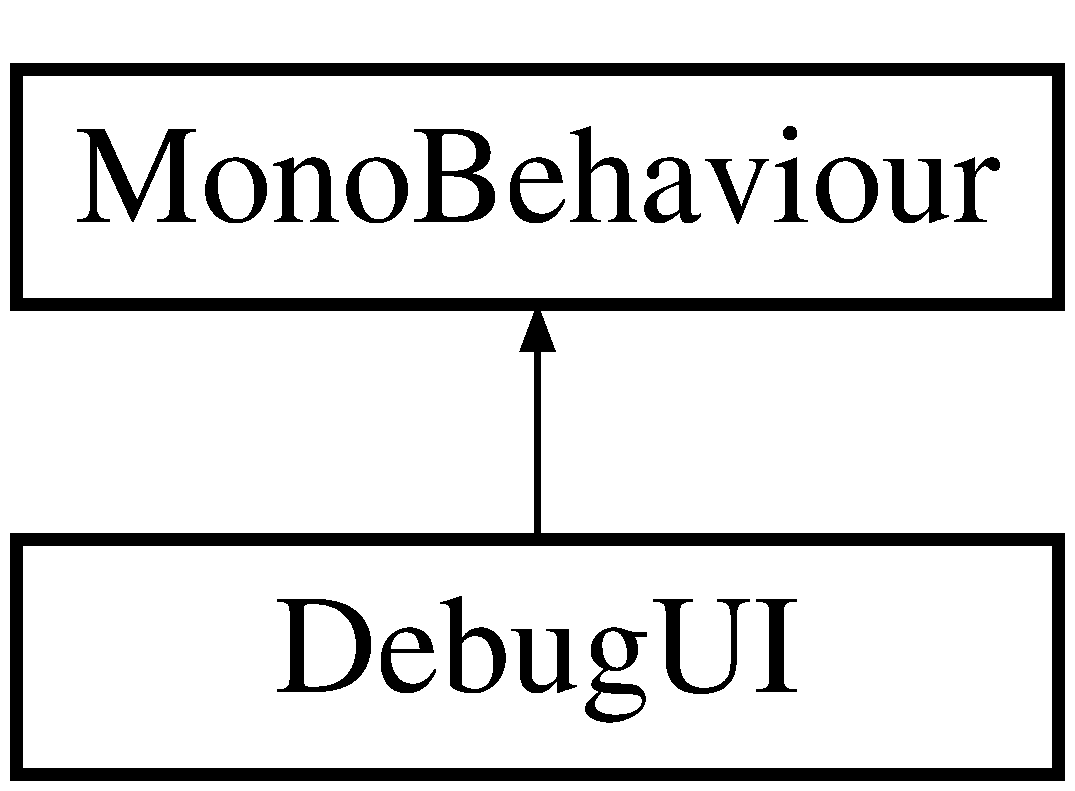
\includegraphics[height=2.000000cm]{class_debug_u_i}
\end{center}
\end{figure}
\subsection*{Private Member Functions}
\begin{DoxyCompactItemize}
\item 
void \hyperlink{group___deb_u_i_unity_ga1369ce8825b055ee93722b2626a06d1e}{Awake} ()
\begin{DoxyCompactList}\small\item\em Initializes the behavior for the button that loads the Audio Testing Interface. \end{DoxyCompactList}\item 
void \hyperlink{group___deb_u_i_handlers_ga16e95ec9c2c6cc4cecf06e54e316f00c}{On\+Go\+To\+A\+T\+I\+Button\+Clicked} ()
\begin{DoxyCompactList}\small\item\em Loads the Audio Testing Interface. \end{DoxyCompactList}\end{DoxyCompactItemize}
\subsection*{Private Attributes}
\begin{DoxyCompactItemize}
\item 
Button \hyperlink{group___deb_u_i_priv_var_gaf9bf8d3b03e88b32bf6a567cd95dfafb}{m\+Go\+To\+A\+T\+I\+Button} = null
\begin{DoxyCompactList}\small\item\em The button to load the Audio Testing Interface. \end{DoxyCompactList}\end{DoxyCompactItemize}


\subsection{Detailed Description}
Handles the UI used for debugging in the Keyboard\+Scene. 

Definition at line 12 of file Debug\+U\+I.\+cs.



The documentation for this class was generated from the following file\+:\begin{DoxyCompactItemize}
\item 
D\+:/\+Documents/\+School Documents/2017\+Spring/\+E\+E\+C\+S542/\+V\+R\+Piano\+Project/\+Assets/\+Scripts/\+Graphics/\hyperlink{_debug_u_i_8cs}{Debug\+U\+I.\+cs}\end{DoxyCompactItemize}

\hypertarget{class_drum_kit}{}\section{Drum\+Kit Class Reference}
\label{class_drum_kit}\index{Drum\+Kit@{Drum\+Kit}}
Inheritance diagram for Drum\+Kit\+:\begin{figure}[H]
\begin{center}
\leavevmode
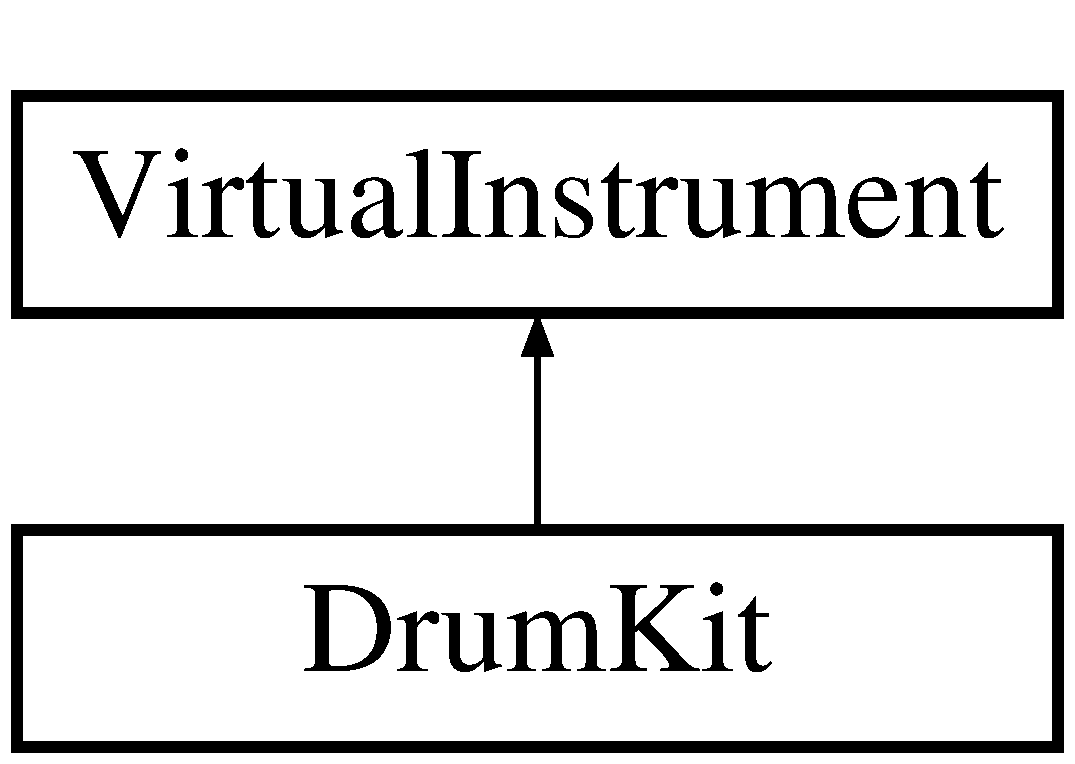
\includegraphics[height=2.000000cm]{class_drum_kit}
\end{center}
\end{figure}
\subsection*{Public Member Functions}
\begin{DoxyCompactItemize}
\item 
\hyperlink{class_drum_kit_abade574e7f9d5684653c0b33524362a7}{Drum\+Kit} (\hyperlink{class_virtual_instrument_manager}{Virtual\+Instrument\+Manager} a\+Parent)
\end{DoxyCompactItemize}
\subsection*{Protected Member Functions}
\begin{DoxyCompactItemize}
\item 
override void \hyperlink{class_drum_kit_ad14c6155e6ec62f26a30261e273d6379}{Initialize\+Built\+In\+Dynamics} ()
\begin{DoxyCompactList}\small\item\em Initializes variables related to \hyperlink{group___audio_DefBID}{Built-\/\+In Dynamics}. \end{DoxyCompactList}\item 
override void \hyperlink{class_drum_kit_a25bb92cf56bc1b3434465faf73cd09cf}{Create\+Filenames} ()
\begin{DoxyCompactList}\small\item\em Creates the filenames for the sample files. \end{DoxyCompactList}\end{DoxyCompactItemize}
\subsection*{Additional Inherited Members}


\subsection{Detailed Description}


Definition at line 16 of file Drum\+Kit.\+cs.



\subsection{Constructor \& Destructor Documentation}
\mbox{\Hypertarget{class_drum_kit_abade574e7f9d5684653c0b33524362a7}\label{class_drum_kit_abade574e7f9d5684653c0b33524362a7}} 
\index{Drum\+Kit@{Drum\+Kit}!Drum\+Kit@{Drum\+Kit}}
\index{Drum\+Kit@{Drum\+Kit}!Drum\+Kit@{Drum\+Kit}}
\subsubsection{\texorpdfstring{Drum\+Kit()}{DrumKit()}}
{\footnotesize\ttfamily Drum\+Kit.\+Drum\+Kit (\begin{DoxyParamCaption}\item[{\hyperlink{class_virtual_instrument_manager}{Virtual\+Instrument\+Manager}}]{a\+Parent }\end{DoxyParamCaption})}



Definition at line 26 of file Drum\+Kit.\+cs.



References Create\+Filenames(), Initialize\+Built\+In\+Dynamics(), Virtual\+Instrument.\+m\+Highest\+Supported\+Pitch, Virtual\+Instrument.\+m\+Is\+Drum, Virtual\+Instrument.\+m\+Loaded, Virtual\+Instrument.\+m\+Lowest\+Supported\+Pitch, Virtual\+Instrument.\+m\+Num\+Supported\+Pitches, Virtual\+Instrument.\+m\+Sample\+Interval, and Virtual\+Instrument.\+m\+Sample\+Rate.


\begin{DoxyCode}
26                                                        : base( aParent )
27     \{
28 
29         \textcolor{comment}{// Set default values}
30         \hyperlink{group___v_i_base_pro_var_ga47dbd8aa02ab32b8f802adfd2d3d81de}{mIsDrum} = \textcolor{keyword}{true};
31         \hyperlink{group___v_i_base_pro_var_ga3cae52b1bcc0178a8a6b03c7aaf7aac8}{mLowestSupportedPitch} = \hyperlink{class_music}{Music}.\hyperlink{group___music_enums_ga508f69b199ea518f935486c990edac1d}{PITCH}.C0;
32         \hyperlink{group___v_i_base_pro_var_ga61fb2c33b53a0f663047779d7ceb18f3}{mHighestSupportedPitch} = \hyperlink{class_music}{Music}.\hyperlink{group___music_enums_ga508f69b199ea518f935486c990edac1d}{PITCH}.F1;
33         \hyperlink{group___v_i_base_pro_var_gafc759a16324cf9b3f230bcbf040afcd2}{mNumSupportedPitches} = 18;
34         \hyperlink{group___v_i_base_pro_var_ga80b3d2ff29b27698eea6bcf2f8ddc5d7}{mSampleRate} = 44100;
35         \hyperlink{group___v_i_base_pro_var_ga20c1d3d25ea666378d72c833d160ae2e}{mSampleInterval} = 1f / \hyperlink{group___v_i_base_pro_var_ga80b3d2ff29b27698eea6bcf2f8ddc5d7}{mSampleRate};
36 
37         \textcolor{comment}{// Call functions to set the values relating to built-in dynamics and create the filenames for each
       sample.}
38         \hyperlink{class_drum_kit_ad14c6155e6ec62f26a30261e273d6379}{InitializeBuiltInDynamics}();
39         \hyperlink{class_drum_kit_a25bb92cf56bc1b3434465faf73cd09cf}{CreateFilenames}();
40 
41         \textcolor{comment}{// Set that this instrument is loaded.}
42         \hyperlink{group___v_i_base_pro_var_ga8978807d1878db5aae91fbd057c46097}{mLoaded} = \textcolor{keyword}{true};
43 
44     \}
\end{DoxyCode}


\subsection{Member Function Documentation}
\mbox{\Hypertarget{class_drum_kit_a25bb92cf56bc1b3434465faf73cd09cf}\label{class_drum_kit_a25bb92cf56bc1b3434465faf73cd09cf}} 
\index{Drum\+Kit@{Drum\+Kit}!Create\+Filenames@{Create\+Filenames}}
\index{Create\+Filenames@{Create\+Filenames}!Drum\+Kit@{Drum\+Kit}}
\subsubsection{\texorpdfstring{Create\+Filenames()}{CreateFilenames()}}
{\footnotesize\ttfamily override void Drum\+Kit.\+Create\+Filenames (\begin{DoxyParamCaption}{ }\end{DoxyParamCaption})\hspace{0.3cm}{\ttfamily [protected]}, {\ttfamily [virtual]}}



Creates the filenames for the sample files. 



Reimplemented from \hyperlink{group___v_i_base_virt_func_gaacfc9521214176292bfb9665556fb991}{Virtual\+Instrument}.



Definition at line 64 of file Drum\+Kit.\+cs.



References Music.\+Drum\+To\+String(), Virtual\+Instrument.\+m\+Filenames, Virtual\+Instrument.\+m\+Filepath, Virtual\+Instrument.\+m\+Highest\+Supported\+Pitch, Virtual\+Instrument.\+m\+Lowest\+Supported\+Pitch, and Virtual\+Instrument.\+m\+Num\+Files.



Referenced by Drum\+Kit().


\begin{DoxyCode}
65     \{
66         \textcolor{comment}{// Set the base filepath and number of files.}
67         \hyperlink{group___v_i_base_pro_var_gac428224be859933d720a9c533fdb5643}{mFilepath} = \textcolor{stringliteral}{"Audio/VirtualInstrument/DrumKit/Samples/"};
68         \hyperlink{group___v_i_base_pro_var_ga9a602db8c9833ce75d95dd453c27d341}{mNumFiles} = 18;
69 
70         \textcolor{comment}{// Initialize the array of filenames.}
71         \hyperlink{group___v_i_base_pro_var_gab2add474ca506357688b5dd08cac4cb5}{mFilenames} = \textcolor{keyword}{new} \textcolor{keywordtype}{string}[\hyperlink{group___v_i_base_pro_var_ga9a602db8c9833ce75d95dd453c27d341}{mNumFiles}];
72 
73         \textcolor{comment}{// Iterate through each dynamics value and create filenames for each supported note.}
74         \textcolor{keywordtype}{int} index = 0;
75         \textcolor{keywordflow}{for}( \textcolor{keywordtype}{int} i = (\textcolor{keywordtype}{int})\hyperlink{group___v_i_base_pro_var_ga3cae52b1bcc0178a8a6b03c7aaf7aac8}{mLowestSupportedPitch}; i <= (int)
      \hyperlink{group___v_i_base_pro_var_ga61fb2c33b53a0f663047779d7ceb18f3}{mHighestSupportedPitch}; i++ )
76         \{
77             \hyperlink{group___v_i_base_pro_var_gab2add474ca506357688b5dd08cac4cb5}{mFilenames}[index] = \hyperlink{group___v_i_base_pro_var_gac428224be859933d720a9c533fdb5643}{mFilepath} + \hyperlink{class_music}{Music}.
      \hyperlink{group___music_stat_func_gaf5f64ebe9a7e036e07f283e41f26d22b}{DrumToString}( i );
78             index++;
79         \}
80     \}
\end{DoxyCode}
\mbox{\Hypertarget{class_drum_kit_ad14c6155e6ec62f26a30261e273d6379}\label{class_drum_kit_ad14c6155e6ec62f26a30261e273d6379}} 
\index{Drum\+Kit@{Drum\+Kit}!Initialize\+Built\+In\+Dynamics@{Initialize\+Built\+In\+Dynamics}}
\index{Initialize\+Built\+In\+Dynamics@{Initialize\+Built\+In\+Dynamics}!Drum\+Kit@{Drum\+Kit}}
\subsubsection{\texorpdfstring{Initialize\+Built\+In\+Dynamics()}{InitializeBuiltInDynamics()}}
{\footnotesize\ttfamily override void Drum\+Kit.\+Initialize\+Built\+In\+Dynamics (\begin{DoxyParamCaption}{ }\end{DoxyParamCaption})\hspace{0.3cm}{\ttfamily [protected]}, {\ttfamily [virtual]}}



Initializes variables related to \hyperlink{group___audio_DefBID}{Built-\/\+In Dynamics}. 



Reimplemented from \hyperlink{group___v_i_base_virt_func_ga995456c03ee54543b285188c51c29a07}{Virtual\+Instrument}.



Definition at line 51 of file Drum\+Kit.\+cs.



References Virtual\+Instrument.\+m\+Audio\+Data, Music.\+M\+A\+X\+\_\+\+S\+U\+P\+P\+O\+R\+T\+E\+D\+\_\+\+D\+R\+U\+MS, Virtual\+Instrument.\+m\+Built\+In\+Dynamics, Virtual\+Instrument.\+m\+Built\+In\+Dynamics\+Thresholds, and Virtual\+Instrument.\+m\+Num\+Built\+In\+Dynamics.



Referenced by Drum\+Kit().


\begin{DoxyCode}
52     \{
53         \textcolor{comment}{// There are no built-in dynamics for the drum kit (yet).}
54         \hyperlink{group___v_i_base_pro_var_gac265f64f759d267ee1e1680f8d387011}{mNumBuiltInDynamics} = 0;
55         \hyperlink{group___v_i_base_pro_var_ga87961e72f25fbc2256b614a394aa6f13}{mBuiltInDynamics} = null;
56         \hyperlink{group___v_i_base_pro_var_gae3db4264dc2a96e99ea680c6d637e6bf}{mBuiltInDynamicsThresholds} = null;
57 
58         \textcolor{comment}{// Allocate the audio data container.}
59         \hyperlink{group___v_i_base_pro_var_ga52e76d9b74408660584676035a92a2c6}{mAudioData} = \textcolor{keyword}{new} \textcolor{keywordtype}{float}[1][][];
60         \hyperlink{group___v_i_base_pro_var_ga52e76d9b74408660584676035a92a2c6}{mAudioData}[0] = \textcolor{keyword}{new} \textcolor{keywordtype}{float}[\hyperlink{class_music}{Music}.\hyperlink{group___music_constants_gabce1a1ac5b9b6355af6bd7fb3868467a}{MAX\_SUPPORTED\_DRUMS}][];
61     \}
\end{DoxyCode}


The documentation for this class was generated from the following file\+:\begin{DoxyCompactItemize}
\item 
D\+:/\+Documents/\+School Documents/2017\+Spring/\+E\+E\+C\+S542/\+V\+R\+Piano\+Project/\+Assets/\+Scripts/\+Audio/\+Virtual\+Instrument/\hyperlink{_drum_kit_8cs}{Drum\+Kit.\+cs}\end{DoxyCompactItemize}

\hypertarget{class_key_container}{}\section{Key\+Container Class Reference}
\label{class_key_container}\index{Key\+Container@{Key\+Container}}


A container that loads each key object and manages them.  


Inheritance diagram for Key\+Container\+:\begin{figure}[H]
\begin{center}
\leavevmode
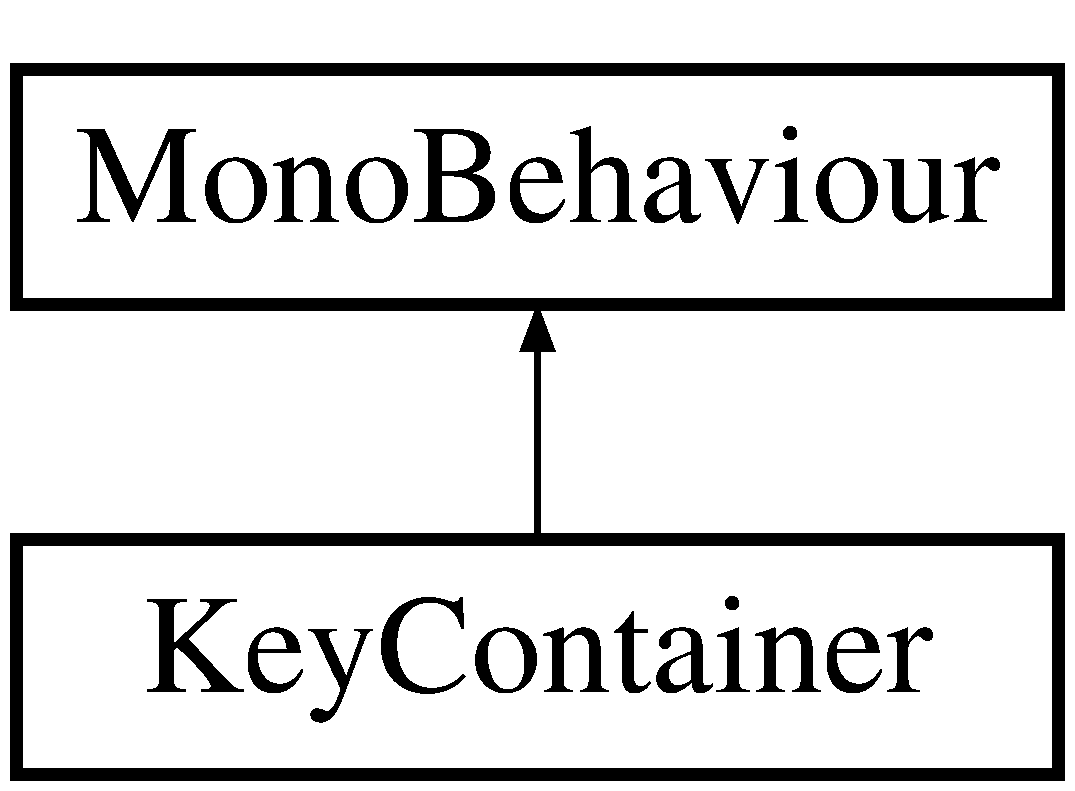
\includegraphics[height=2.000000cm]{class_key_container}
\end{center}
\end{figure}
\subsection*{Public Member Functions}
\begin{DoxyCompactItemize}
\item 
void \hyperlink{group___key_contain_handlers_ga5fc6752f438bda64f0f860da0788fc13}{Handle\+Audio\+Toggle} (bool a\+Audio\+Enabled)
\begin{DoxyCompactList}\small\item\em Allows for other objects to toggle the audio. \end{DoxyCompactList}\end{DoxyCompactItemize}
\subsection*{Public Attributes}
\begin{DoxyCompactItemize}
\item 
bool \hyperlink{group___key_contain_pub_var_ga5dc9b1349f8fafc894c7f739f6780a8c}{Enable\+Audio} = false
\end{DoxyCompactItemize}
\subsection*{Private Member Functions}
\begin{DoxyCompactItemize}
\item 
void \hyperlink{group___key_contain_unity_ga9e307b409b1e07b2be51a21afe5d7379}{Awake} ()
\begin{DoxyCompactList}\small\item\em Initializes the \hyperlink{class_key_container}{Key\+Container} and loads each key. \end{DoxyCompactList}\item 
void \hyperlink{group___key_contain_unity_gae0e513a4ef9fd25c1e0f5f3bc53d9b5c}{Update} ()
\item 
void \hyperlink{group___key_contain_priv_func_ga679f5ca9d6b1505180e90ee00bbfe616}{Clear\+Keyboard} ()
\begin{DoxyCompactList}\small\item\em Clears the keyboard. \end{DoxyCompactList}\item 
void \hyperlink{group___key_contain_priv_func_ga65f79700f265d2223681ac95981ab4a3}{Load\+Keys} ()
\begin{DoxyCompactList}\small\item\em Loads the keys in the container. \end{DoxyCompactList}\item 
void \hyperlink{group___key_contain_handlers_ga05cc2543fd9772b26e27bf4f6247ab47}{Handle\+Black\+Key\+Pressed} (\hyperlink{class_black_key}{Black\+Key} a\+Black\+Key)
\begin{DoxyCompactList}\small\item\em Handles a black key in the container being pressed. \end{DoxyCompactList}\item 
void \hyperlink{group___key_contain_handlers_ga5a0c5565c5ebc6026b3122f487e51704}{Handle\+Black\+Key\+Released} (\hyperlink{class_black_key}{Black\+Key} a\+Black\+Key)
\begin{DoxyCompactList}\small\item\em Handles a black key in the container being released. \end{DoxyCompactList}\item 
void \hyperlink{group___key_contain_handlers_ga0d82098e4f886f77a33f9d5ed13fe195}{Handle\+Change\+Note\+Range\+Event} (\hyperlink{group___music_enums_ga508f69b199ea518f935486c990edac1d}{Music.\+P\+I\+T\+CH} a\+New\+Lowest\+Pitch)
\begin{DoxyCompactList}\small\item\em Handles \hyperlink{group___v_i_m_event_types_class_virtual_instrument_manager_1_1_change_note_range_event}{a change in the note range}. \end{DoxyCompactList}\item 
void \hyperlink{group___key_contain_handlers_ga4e2c5e8be389a7514429910e7d61f028}{Handle\+White\+Key\+Pressed} (\hyperlink{class_white_key}{White\+Key} a\+White\+Key)
\begin{DoxyCompactList}\small\item\em Handles a white key in the container being pressed. \end{DoxyCompactList}\item 
void \hyperlink{group___key_contain_handlers_ga5b98b0105300225fd79638525ad3cb3c}{Handle\+White\+Key\+Released} (\hyperlink{class_white_key}{White\+Key} a\+White\+Key)
\begin{DoxyCompactList}\small\item\em Handles a white key in the container being released. \end{DoxyCompactList}\item 
void \hyperlink{group___key_contain_handlers_ga894c823059c5268af0954f83c04036ed}{Handle\+Play\+Song\+Event} (\hyperlink{class_song}{Song} a\+Song)
\begin{DoxyCompactList}\small\item\em Handler for when a song begins playing. \end{DoxyCompactList}\item 
I\+Enumerator \hyperlink{group___key_contain_handlers_gac6b82feca83eaf5e3ce6901088bc552c}{Draw\+Lesson\+Marker} (int a\+Index, float a\+Delay, float a\+Stop)
\begin{DoxyCompactList}\small\item\em Handles drawing the lesson markers. \end{DoxyCompactList}\end{DoxyCompactItemize}
\subsection*{Private Attributes}
\begin{DoxyCompactItemize}
\item 
const int \hyperlink{group___key_contain_const_gaa8fe6473e6396976e52c5793f027380e}{N\+U\+M\+\_\+\+K\+E\+YS} = 25
\begin{DoxyCompactList}\small\item\em The default number of keys shown. \end{DoxyCompactList}\item 
const string \hyperlink{group___key_contain_const_gac968b0d398c545a13abad255d8287825}{B\+L\+A\+C\+K\+\_\+\+K\+E\+Y\+\_\+\+P\+A\+TH} = \char`\"{}Graphics/Prefabs/Black\+Key\+Prefab\char`\"{}
\begin{DoxyCompactList}\small\item\em The path to load the prefab for the black keys. \end{DoxyCompactList}\item 
const string \hyperlink{group___key_contain_const_ga4caccd17bb57caca66047951046aa44a}{L\+E\+S\+S\+O\+N\+\_\+\+M\+A\+R\+K\+E\+R\+\_\+\+P\+A\+TH} = \char`\"{}Audio/Prefabs/Lesson\+Marker\+Prefab\char`\"{}
\begin{DoxyCompactList}\small\item\em The path to load a lesson marker. \end{DoxyCompactList}\item 
const string \hyperlink{group___key_contain_const_ga8dc749271ab095b5759129459bcb647a}{V\+I\+M\+\_\+\+P\+A\+TH} = \char`\"{}Audio/Prefabs/Virtual\+Instrument\+Manager\+Prefab\char`\"{}
\begin{DoxyCompactList}\small\item\em The path to load the \hyperlink{group___v_i_m}{Virtual Instrument Manager}. \end{DoxyCompactList}\item 
const string \hyperlink{group___key_contain_const_ga8ce7e53d5c067095ee26b96fcc522584}{W\+H\+I\+T\+E\+\_\+\+K\+E\+Y\+\_\+\+P\+A\+TH} = \char`\"{}Graphics/Prefabs/White\+Key\+Prefab\char`\"{}
\begin{DoxyCompactList}\small\item\em The path to load the prefab for the white keys. \end{DoxyCompactList}\item 
float \hyperlink{group___key_contain_priv_var_ga6461d765c3904e6a3031558d7385be25}{m\+Black\+Key\+Width} = 0f
\begin{DoxyCompactList}\small\item\em The width of a black key. \end{DoxyCompactList}\item 
float \hyperlink{group___key_contain_priv_var_gae5b8787a5242834f99ad8072e7ea6004}{m\+White\+Key\+Width} = 0f
\begin{DoxyCompactList}\small\item\em The width of a white key. \end{DoxyCompactList}\item 
Game\+Object \mbox{[}$\,$\mbox{]} \hyperlink{group___key_contain_priv_var_ga01addf187bb12ffe824374df98e2c2d8}{m\+Key\+Objects} = null
\begin{DoxyCompactList}\small\item\em The keys held in the container. Need to update this once the classes are combined. \end{DoxyCompactList}\item 
Game\+Object \mbox{[}$\,$\mbox{]} \hyperlink{group___key_contain_priv_var_gaf21490115ecf2b80c1bd382d7469a08c}{m\+Lesson\+Markers} = null
\begin{DoxyCompactList}\small\item\em Lesson markers for showing which key to hit. Just testing this for now to see if I can get the audio timing right. \end{DoxyCompactList}\item 
int \hyperlink{group___key_contain_priv_var_ga7a5547a1fe5c40eac487fe6c826c8f9c}{m\+Num\+White\+Keys} = 0
\begin{DoxyCompactList}\small\item\em The number of white keys being shown. Used for positioning. \end{DoxyCompactList}\item 
\hyperlink{group___music_enums_ga508f69b199ea518f935486c990edac1d}{Music.\+P\+I\+T\+CH} \mbox{[}$\,$\mbox{]} \hyperlink{group___key_contain_priv_var_ga103945a6efe3469191e5253d13fec5be}{m\+Represented\+Pitches} = null
\begin{DoxyCompactList}\small\item\em The pitches that are represented by the keyboard. \end{DoxyCompactList}\item 
\hyperlink{class_virtual_instrument_manager}{Virtual\+Instrument\+Manager} \hyperlink{group___key_contain_priv_var_ga57ee3824e2f284403bb70ad9c4dfd307}{m\+V\+IM} = null
\begin{DoxyCompactList}\small\item\em The bridge to the audio code. \end{DoxyCompactList}\end{DoxyCompactItemize}


\subsection{Detailed Description}
A container that loads each key object and manages them. 

Definition at line 12 of file Key\+Container.\+cs.



The documentation for this class was generated from the following file\+:\begin{DoxyCompactItemize}
\item 
D\+:/\+Documents/\+School Documents/2017\+Spring/\+E\+E\+C\+S542/\+V\+R\+Piano\+Project/\+Assets/\+Scripts/\+Graphics/\hyperlink{_key_container_8cs}{Key\+Container.\+cs}\end{DoxyCompactItemize}

\hypertarget{class_marimba}{}\section{Marimba Class Reference}
\label{class_marimba}\index{Marimba@{Marimba}}


A specific type of \hyperlink{group___v_i}{Virtual Instrument} that uses marimba samples.  


Inheritance diagram for Marimba\+:\begin{figure}[H]
\begin{center}
\leavevmode
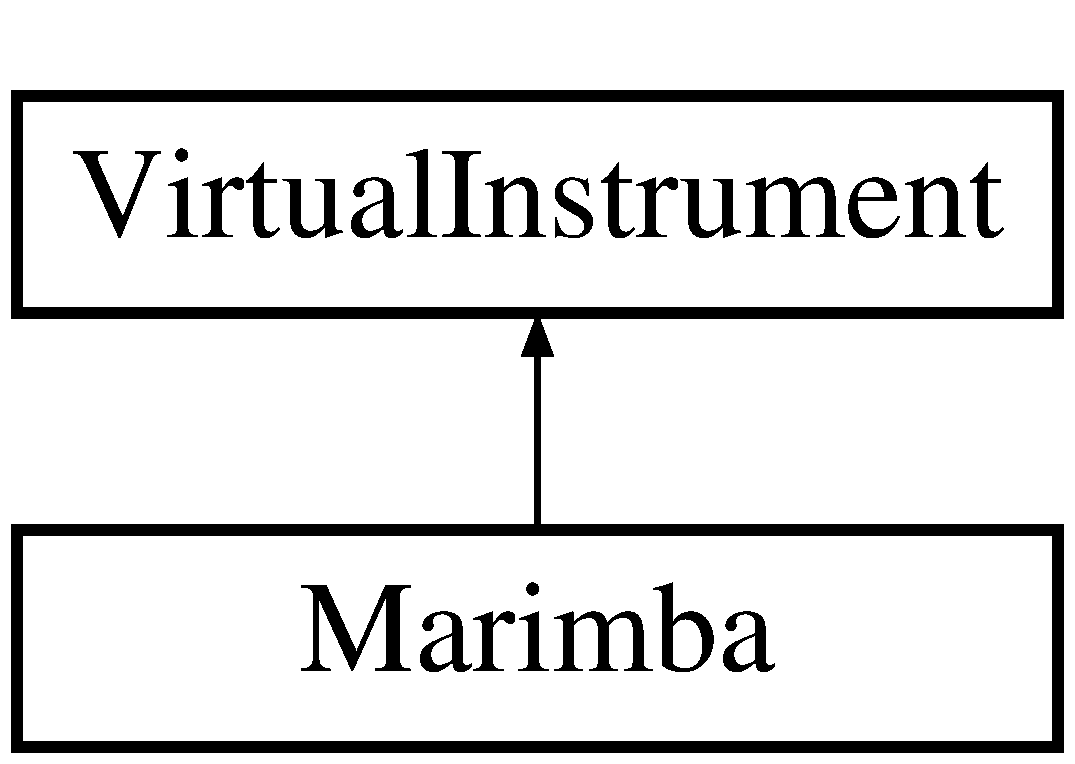
\includegraphics[height=2.000000cm]{class_marimba}
\end{center}
\end{figure}
\subsection*{Public Member Functions}
\begin{DoxyCompactItemize}
\item 
\hyperlink{group___mar_construct_ga48c946fe0f78f8905a8e4d063cbc0fa2}{Marimba} (\hyperlink{class_virtual_instrument_manager}{Virtual\+Instrument\+Manager} a\+Parent)
\begin{DoxyCompactList}\small\item\em Creates a new \hyperlink{class_marimba}{Marimba} instance. \end{DoxyCompactList}\end{DoxyCompactItemize}
\subsection*{Protected Member Functions}
\begin{DoxyCompactItemize}
\item 
override void \hyperlink{group___mar_virt_func_ga293d829cb8571c21452c23e90968b2d8}{Initialize\+Built\+In\+Dynamics} ()
\begin{DoxyCompactList}\small\item\em Initializes values related to the \hyperlink{group___audio_DefBID}{Built-\/\+In Dynamics} for this instrument. \end{DoxyCompactList}\item 
override void \hyperlink{group___mar_virt_func_gae57d9737fd07708dc7e13e74ee777878}{Create\+Filenames} ()
\begin{DoxyCompactList}\small\item\em Creates the filenames of the W\+AV files used to create the \hyperlink{class_marimba}{Marimba}. \end{DoxyCompactList}\end{DoxyCompactItemize}
\subsection*{Additional Inherited Members}


\subsection{Detailed Description}
A specific type of \hyperlink{group___v_i}{Virtual Instrument} that uses marimba samples. 

The lowest supported \hyperlink{group___music_enums_ga508f69b199ea518f935486c990edac1d}{pitch} of the marimba is \hyperlink{group___music_enums_gga508f69b199ea518f935486c990edac1daf1a543f5a2c5d49bc5dde298fcf716e4}{C2}. ~\newline
 The highest supported \hyperlink{group___music_enums_ga508f69b199ea518f935486c990edac1d}{pitch} of the marimba is \hyperlink{group___music_enums_gga508f69b199ea518f935486c990edac1da517d42f048d2dd422533522c796aaf37}{C7}. ~\newline
 The marimba does not support \hyperlink{group___audio_DefBID}{Built-\/\+In Dynamics}. 

Definition at line 15 of file Marimba.\+cs.



The documentation for this class was generated from the following file\+:\begin{DoxyCompactItemize}
\item 
D\+:/\+Documents/\+School Documents/2017\+Spring/\+E\+E\+C\+S542/\+V\+R\+Piano\+Project/\+Assets/\+Scripts/\+Audio/\+Virtual\+Instrument/\hyperlink{_marimba_8cs}{Marimba.\+cs}\end{DoxyCompactItemize}

\hypertarget{class_music}{}\section{Music Class Reference}
\label{class_music}\index{Music@{Music}}


A container for everything related to music such as pitches and note lengths. This class does not need to be initialized to use.  


\subsection*{Classes}
\begin{DoxyCompactItemize}
\item 
struct \hyperlink{group___music_structs_struct_music_1_1_combined_note}{Combined\+Note}
\begin{DoxyCompactList}\small\item\em A struct that provides an abstract representation of a note that has both drums and melody.  \hyperlink{group___music_structs_struct_music_1_1_combined_note}{More...}\end{DoxyCompactList}\item 
struct \hyperlink{group___music_structs_struct_music_1_1_melody_note}{Melody\+Note}
\begin{DoxyCompactList}\small\item\em A struct that provides an abstract representation of a note for a non-\/\+Drum\+Kit \hyperlink{class_virtual_instrument}{Virtual\+Instrument}.  \hyperlink{group___music_structs_struct_music_1_1_melody_note}{More...}\end{DoxyCompactList}\item 
struct \hyperlink{group___music_structs_struct_music_1_1_percussion_note}{Percussion\+Note}
\begin{DoxyCompactList}\small\item\em A struct that provides an abstract representation of a note for a \hyperlink{class_drum_kit}{Drum\+Kit}.  \hyperlink{group___music_structs_struct_music_1_1_percussion_note}{More...}\end{DoxyCompactList}\item 
struct \hyperlink{group___music_structs_struct_music_1_1_time_signature}{Time\+Signature}
\begin{DoxyCompactList}\small\item\em A struct that represents a time signature.  \hyperlink{group___music_structs_struct_music_1_1_time_signature}{More...}\end{DoxyCompactList}\end{DoxyCompactItemize}
\subsection*{Public Types}
\begin{DoxyCompactItemize}
\item 
enum \hyperlink{group___music_enums_gade475b4382c7066d1af13e7c13c029b6}{D\+R\+UM} \{ \newline
\hyperlink{group___music_enums_ggade475b4382c7066d1af13e7c13c029b6a871b243e59015ac599015e9c5f8cfdaa}{D\+R\+U\+M.\+K\+I\+C\+K\+\_\+1}, 
\hyperlink{group___music_enums_ggade475b4382c7066d1af13e7c13c029b6add8ac581cd99ea05f540393daaba0be5}{D\+R\+U\+M.\+K\+I\+C\+K\+\_\+2}, 
\hyperlink{group___music_enums_ggade475b4382c7066d1af13e7c13c029b6a30d844bdad6320b2c056a8d37583b178}{D\+R\+U\+M.\+S\+N\+A\+R\+E\+\_\+1}, 
\hyperlink{group___music_enums_ggade475b4382c7066d1af13e7c13c029b6ac0944af51708424f9ecfcaf6b9ceb40b}{D\+R\+U\+M.\+S\+N\+A\+R\+E\+\_\+\+R\+IM}, 
\hyperlink{group___music_enums_ggade475b4382c7066d1af13e7c13c029b6adf63db786582e77fbec3d22acfbb2c26}{D\+R\+U\+M.\+S\+N\+A\+R\+E\+\_\+2}, 
\hyperlink{group___music_enums_ggade475b4382c7066d1af13e7c13c029b6ab169d27f8ff1efb87d58da212b6bc25a}{D\+R\+U\+M.\+L\+O\+W\+T\+O\+M\+\_\+1}, 
\hyperlink{group___music_enums_ggade475b4382c7066d1af13e7c13c029b6aa19f835d81e001ed1084d75dcf79e9e1}{D\+R\+U\+M.\+H\+I\+H\+A\+T\+\_\+C}, 
\hyperlink{group___music_enums_ggade475b4382c7066d1af13e7c13c029b6a427f3138018251643177388299d9b3d3}{D\+R\+U\+M.\+L\+O\+W\+T\+O\+M\+\_\+2}, 
\hyperlink{group___music_enums_ggade475b4382c7066d1af13e7c13c029b6a1f0a3efea7dc89dc7364d7ada15332c7}{D\+R\+U\+M.\+H\+I\+H\+A\+T\+\_\+P}, 
\hyperlink{group___music_enums_ggade475b4382c7066d1af13e7c13c029b6a7cfe02c9cff874222e8e298e78338181}{D\+R\+U\+M.\+M\+I\+D\+T\+O\+M\+\_\+1}, 
\hyperlink{group___music_enums_ggade475b4382c7066d1af13e7c13c029b6a5da9560603e1755c936289eda0c9d46b}{D\+R\+U\+M.\+H\+I\+H\+A\+T\+\_\+O}, 
\hyperlink{group___music_enums_ggade475b4382c7066d1af13e7c13c029b6ae24e4cd397daacac51069cb4209d075c}{D\+R\+U\+M.\+M\+I\+D\+T\+O\+M\+\_\+2}, 
\newline
\hyperlink{group___music_enums_ggade475b4382c7066d1af13e7c13c029b6a5542bef9b7c7387048a53df9c956815b}{D\+R\+U\+M.\+H\+I\+G\+H\+T\+O\+M\+\_\+1}, 
\hyperlink{group___music_enums_ggade475b4382c7066d1af13e7c13c029b6a5cc345cd6dde1f871f706f00b8d3389e}{D\+R\+U\+M.\+C\+R\+A\+S\+H\+\_\+1}, 
\hyperlink{group___music_enums_ggade475b4382c7066d1af13e7c13c029b6aea2fc79b38ff3fc96f9ee77f6a05eb78}{D\+R\+U\+M.\+H\+I\+G\+H\+T\+O\+M\+\_\+2}, 
\hyperlink{group___music_enums_ggade475b4382c7066d1af13e7c13c029b6a82def663d0a5065e52c86a3d9f462054}{D\+R\+U\+M.\+R\+I\+DE}, 
\hyperlink{group___music_enums_ggade475b4382c7066d1af13e7c13c029b6ab22cbce9616b64f3a24f5df4b81c178f}{D\+R\+U\+M.\+C\+R\+A\+S\+H\+\_\+2}, 
\hyperlink{group___music_enums_ggade475b4382c7066d1af13e7c13c029b6a2259a8afe41c9293034e327a24a550bd}{D\+R\+U\+M.\+R\+I\+D\+E\+\_\+\+B\+E\+LL}
 \}\begin{DoxyCompactList}\small\item\em The possible drums/cymbals that can be played. \end{DoxyCompactList}
\item 
enum \hyperlink{group___music_enums_gabfce60192305965558a36e368ebd67c3}{I\+N\+S\+T\+R\+U\+M\+E\+N\+T\+\_\+\+T\+Y\+PE} \{ \hyperlink{group___music_enums_ggabfce60192305965558a36e368ebd67c3aef6dcf375679288e8fe520ec07f29130}{I\+N\+S\+T\+R\+U\+M\+E\+N\+T\+\_\+\+T\+Y\+P\+E.\+P\+I\+A\+NO}, 
\hyperlink{group___music_enums_ggabfce60192305965558a36e368ebd67c3ae84dbd9f12bf5278bfa76a692e42f50f}{I\+N\+S\+T\+R\+U\+M\+E\+N\+T\+\_\+\+T\+Y\+P\+E.\+M\+A\+R\+I\+M\+BA}, 
\hyperlink{group___music_enums_ggabfce60192305965558a36e368ebd67c3aceaaf30d57fed4b1c3f4b95c60a76df6}{I\+N\+S\+T\+R\+U\+M\+E\+N\+T\+\_\+\+T\+Y\+P\+E.\+D\+R\+U\+M\+\_\+\+K\+IT}
 \}\begin{DoxyCompactList}\small\item\em The types of instruments that are currently supported. \end{DoxyCompactList}
\item 
enum \hyperlink{group___music_enums_gaf11b5f079adbb21c800b9eca1c5c3cbd}{N\+O\+T\+E\+\_\+\+L\+E\+N\+G\+TH} \{ \newline
\hyperlink{group___music_enums_ggaf11b5f079adbb21c800b9eca1c5c3cbdab9ece18c950afbfa6b0fdbfa4ff731d3}{N\+O\+T\+E\+\_\+\+L\+E\+N\+G\+T\+H.\+T}, 
\hyperlink{group___music_enums_ggaf11b5f079adbb21c800b9eca1c5c3cbda5965eb90b97091e4c04c3e63c8cadc82}{N\+O\+T\+E\+\_\+\+L\+E\+N\+G\+T\+H.\+D\+\_\+T}, 
\hyperlink{group___music_enums_ggaf11b5f079adbb21c800b9eca1c5c3cbda5dbc98dcc983a70728bd082d1a47546e}{N\+O\+T\+E\+\_\+\+L\+E\+N\+G\+T\+H.\+S}, 
\hyperlink{group___music_enums_ggaf11b5f079adbb21c800b9eca1c5c3cbda99bc05b985a6557303572f10feeb65e8}{N\+O\+T\+E\+\_\+\+L\+E\+N\+G\+T\+H.\+D\+\_\+S}, 
\hyperlink{group___music_enums_ggaf11b5f079adbb21c800b9eca1c5c3cbda3a3ea00cfc35332cedf6e5e9a32e94da}{N\+O\+T\+E\+\_\+\+L\+E\+N\+G\+T\+H.\+E}, 
\hyperlink{group___music_enums_ggaf11b5f079adbb21c800b9eca1c5c3cbdad1045a0cd40aaa2adbfa3492d2a1d8a6}{N\+O\+T\+E\+\_\+\+L\+E\+N\+G\+T\+H.\+D\+\_\+E}, 
\hyperlink{group___music_enums_ggaf11b5f079adbb21c800b9eca1c5c3cbdaf09564c9ca56850d4cd6b3319e541aee}{N\+O\+T\+E\+\_\+\+L\+E\+N\+G\+T\+H.\+Q}, 
\hyperlink{group___music_enums_ggaf11b5f079adbb21c800b9eca1c5c3cbda13f258ec288ede9f0f778903d707d8f5}{N\+O\+T\+E\+\_\+\+L\+E\+N\+G\+T\+H.\+D\+\_\+Q}, 
\hyperlink{group___music_enums_ggaf11b5f079adbb21c800b9eca1c5c3cbdac1d9f50f86825a1a2302ec2449c17196}{N\+O\+T\+E\+\_\+\+L\+E\+N\+G\+T\+H.\+H}, 
\hyperlink{group___music_enums_ggaf11b5f079adbb21c800b9eca1c5c3cbda4365f24e724bf9109fb51285a7e8d709}{N\+O\+T\+E\+\_\+\+L\+E\+N\+G\+T\+H.\+D\+\_\+H}, 
\hyperlink{group___music_enums_ggaf11b5f079adbb21c800b9eca1c5c3cbda61e9c06ea9a85a5088a499df6458d276}{N\+O\+T\+E\+\_\+\+L\+E\+N\+G\+T\+H.\+W}, 
\hyperlink{group___music_enums_ggaf11b5f079adbb21c800b9eca1c5c3cbda65c5afa16a4bd2e074686f5a864f1cf8}{N\+O\+T\+E\+\_\+\+L\+E\+N\+G\+T\+H.\+D\+\_\+W}, 
\newline
\hyperlink{group___music_enums_ggaf11b5f079adbb21c800b9eca1c5c3cbdab50339a10e1de285ac99d4c3990b8693}{N\+O\+T\+E\+\_\+\+L\+E\+N\+G\+T\+H.\+N\+O\+NE}
 \}\begin{DoxyCompactList}\small\item\em Abstract representations of a note\textquotesingle{}s length. \end{DoxyCompactList}
\item 
enum \hyperlink{group___music_enums_ga508f69b199ea518f935486c990edac1d}{P\+I\+T\+CH} \{ \newline
\hyperlink{group___music_enums_gga508f69b199ea518f935486c990edac1da9c5959e6f08f10d0edbadf5be1f33c53}{P\+I\+T\+C\+H.\+C0}, 
\hyperlink{group___music_enums_gga508f69b199ea518f935486c990edac1da148deee61c02bd1bb71c270396d62b04}{P\+I\+T\+C\+H.\+C\+S0}, 
\hyperlink{group___music_enums_gga508f69b199ea518f935486c990edac1da0e3e06c992d1ead056a6861bb46b28a8}{P\+I\+T\+C\+H.\+D0}, 
\hyperlink{group___music_enums_gga508f69b199ea518f935486c990edac1da02b462a08c9441274297c5edd4031595}{P\+I\+T\+C\+H.\+D\+S0}, 
\hyperlink{group___music_enums_gga508f69b199ea518f935486c990edac1da0e51a87ec173dd9534a056a403c85881}{P\+I\+T\+C\+H.\+E0}, 
\hyperlink{group___music_enums_gga508f69b199ea518f935486c990edac1daee0c8bd6520d8fb37a28c61189d0e821}{P\+I\+T\+C\+H.\+F0}, 
\hyperlink{group___music_enums_gga508f69b199ea518f935486c990edac1da1848af1387dd6164523bc6a1e6b3e09b}{P\+I\+T\+C\+H.\+F\+S0}, 
\hyperlink{group___music_enums_gga508f69b199ea518f935486c990edac1da22294e216be9e629e37caf9fa0cc5872}{P\+I\+T\+C\+H.\+G0}, 
\hyperlink{group___music_enums_gga508f69b199ea518f935486c990edac1da4060fa5b6da9486d34fe421842df5da2}{P\+I\+T\+C\+H.\+G\+S0}, 
\hyperlink{group___music_enums_gga508f69b199ea518f935486c990edac1dad88c146dfafdea37a837778a92415bc2}{P\+I\+T\+C\+H.\+A0}, 
\hyperlink{group___music_enums_gga508f69b199ea518f935486c990edac1da60332432d378cfdc1afcbeb6aace0ca0}{P\+I\+T\+C\+H.\+A\+S0}, 
\hyperlink{group___music_enums_gga508f69b199ea518f935486c990edac1da4c769c2c9989abb9fa024ab9930270e5}{P\+I\+T\+C\+H.\+B0}, 
\newline
\hyperlink{group___music_enums_gga508f69b199ea518f935486c990edac1da1a2ddc2db4693cfd16d534cde5572cc1}{P\+I\+T\+C\+H.\+C1}, 
\hyperlink{group___music_enums_gga508f69b199ea518f935486c990edac1da8ea4c9ac938645ff943aeb7a9c2bc060}{P\+I\+T\+C\+H.\+C\+S1}, 
\hyperlink{group___music_enums_gga508f69b199ea518f935486c990edac1da4a4079e06eb2f7ba7a12821c7c58a3f6}{P\+I\+T\+C\+H.\+D1}, 
\hyperlink{group___music_enums_gga508f69b199ea518f935486c990edac1da3f30b4c23d5d31403db81c95f79160f9}{P\+I\+T\+C\+H.\+D\+S1}, 
\hyperlink{group___music_enums_gga508f69b199ea518f935486c990edac1da48ed5d2db39237d7ae5e829b17581629}{P\+I\+T\+C\+H.\+E1}, 
\hyperlink{group___music_enums_gga508f69b199ea518f935486c990edac1dae1dffc8709f31a4987c8a88334107e89}{P\+I\+T\+C\+H.\+F1}, 
\hyperlink{group___music_enums_gga508f69b199ea518f935486c990edac1da7d4883feac2c828238c29cf184665348}{P\+I\+T\+C\+H.\+F\+S1}, 
\hyperlink{group___music_enums_gga508f69b199ea518f935486c990edac1dac0497521d35d66866e3af408094864c3}{P\+I\+T\+C\+H.\+G1}, 
\hyperlink{group___music_enums_gga508f69b199ea518f935486c990edac1dacf301661e1df9727a6c2c6c963c49d55}{P\+I\+T\+C\+H.\+G\+S1}, 
\hyperlink{group___music_enums_gga508f69b199ea518f935486c990edac1da27f237e6b7f96587b6202ff3607ad88a}{P\+I\+T\+C\+H.\+A1}, 
\hyperlink{group___music_enums_gga508f69b199ea518f935486c990edac1dacf0ac41ddff111e8299e51e12417f7bf}{P\+I\+T\+C\+H.\+A\+S1}, 
\hyperlink{group___music_enums_gga508f69b199ea518f935486c990edac1dac9512565ef6194ca664dc41ec0de7a53}{P\+I\+T\+C\+H.\+B1}, 
\newline
\hyperlink{group___music_enums_gga508f69b199ea518f935486c990edac1daf1a543f5a2c5d49bc5dde298fcf716e4}{P\+I\+T\+C\+H.\+C2}, 
\hyperlink{group___music_enums_gga508f69b199ea518f935486c990edac1daaef7a4e1b7e3fe7e4df67684dbffa9e1}{P\+I\+T\+C\+H.\+C\+S2}, 
\hyperlink{group___music_enums_gga508f69b199ea518f935486c990edac1dac4d62b6dcca08e5caf06c01889282859}{P\+I\+T\+C\+H.\+D2}, 
\hyperlink{group___music_enums_gga508f69b199ea518f935486c990edac1dac92b438c6de07b10e6b5ce6dcb9961c9}{P\+I\+T\+C\+H.\+D\+S2}, 
\hyperlink{group___music_enums_gga508f69b199ea518f935486c990edac1da560fce20abef5cd3f8e4d13c94669a46}{P\+I\+T\+C\+H.\+E2}, 
\hyperlink{group___music_enums_gga508f69b199ea518f935486c990edac1dafe5c3684dce76cdd9f7f42430868aa74}{P\+I\+T\+C\+H.\+F2}, 
\hyperlink{group___music_enums_gga508f69b199ea518f935486c990edac1daa43bf0ad8387aed475b73432a959e196}{P\+I\+T\+C\+H.\+F\+S2}, 
\hyperlink{group___music_enums_gga508f69b199ea518f935486c990edac1dad24bade136bc8cd77e37395ea94226eb}{P\+I\+T\+C\+H.\+G2}, 
\hyperlink{group___music_enums_gga508f69b199ea518f935486c990edac1dabb7e8732afc60ab2c8d68b9f00890e80}{P\+I\+T\+C\+H.\+G\+S2}, 
\hyperlink{group___music_enums_gga508f69b199ea518f935486c990edac1dac6bdf6f65f3845da9085e9ae5790b494}{P\+I\+T\+C\+H.\+A2}, 
\hyperlink{group___music_enums_gga508f69b199ea518f935486c990edac1da59cdaab533f69062f6fbdde53f047c03}{P\+I\+T\+C\+H.\+A\+S2}, 
\hyperlink{group___music_enums_gga508f69b199ea518f935486c990edac1dabbd97b00c539801e32317ab550867ec4}{P\+I\+T\+C\+H.\+B2}, 
\newline
\hyperlink{group___music_enums_gga508f69b199ea518f935486c990edac1da3abe124ecc82bf2c2e22e6058f38c50c}{P\+I\+T\+C\+H.\+C3}, 
\hyperlink{group___music_enums_gga508f69b199ea518f935486c990edac1da8c4e56414e26520294c3b571e92e58e4}{P\+I\+T\+C\+H.\+C\+S3}, 
\hyperlink{group___music_enums_gga508f69b199ea518f935486c990edac1daa3deb6e481689f1d3303caecb8a6c401}{P\+I\+T\+C\+H.\+D3}, 
\hyperlink{group___music_enums_gga508f69b199ea518f935486c990edac1daedeca07ff932c4c2713e8a44f508ccad}{P\+I\+T\+C\+H.\+D\+S3}, 
\hyperlink{group___music_enums_gga508f69b199ea518f935486c990edac1dab29bcbb0f188e0093434a5f213285f46}{P\+I\+T\+C\+H.\+E3}, 
\hyperlink{group___music_enums_gga508f69b199ea518f935486c990edac1da4b6bf4b531770872d4328ce69bef5627}{P\+I\+T\+C\+H.\+F3}, 
\hyperlink{group___music_enums_gga508f69b199ea518f935486c990edac1da2f0912f92c162d890ce3533b79502f07}{P\+I\+T\+C\+H.\+F\+S3}, 
\hyperlink{group___music_enums_gga508f69b199ea518f935486c990edac1dabc75ca3e24efaf835d947dbe27a95c8a}{P\+I\+T\+C\+H.\+G3}, 
\hyperlink{group___music_enums_gga508f69b199ea518f935486c990edac1daf32c267184e725aa6224dcde41d4c1d0}{P\+I\+T\+C\+H.\+G\+S3}, 
\hyperlink{group___music_enums_gga508f69b199ea518f935486c990edac1da6593d7b12fd418cdb35bbf438de72f66}{P\+I\+T\+C\+H.\+A3}, 
\hyperlink{group___music_enums_gga508f69b199ea518f935486c990edac1da84af1c48f92dad5d3c09a15bba7fa031}{P\+I\+T\+C\+H.\+A\+S3}, 
\hyperlink{group___music_enums_gga508f69b199ea518f935486c990edac1da0c4ecd7b59ebc5b9f47974cb9845fd02}{P\+I\+T\+C\+H.\+B3}, 
\newline
\hyperlink{group___music_enums_gga508f69b199ea518f935486c990edac1dab713e6323a68d3ddabf4855826c50148}{P\+I\+T\+C\+H.\+C4}, 
\hyperlink{group___music_enums_gga508f69b199ea518f935486c990edac1da7009daf81333670cd06b8bb2b02054cc}{P\+I\+T\+C\+H.\+C\+S4}, 
\hyperlink{group___music_enums_gga508f69b199ea518f935486c990edac1da2521dc256a4368da87585c936b451dd7}{P\+I\+T\+C\+H.\+D4}, 
\hyperlink{group___music_enums_gga508f69b199ea518f935486c990edac1dac55d4e2df1d19210fbdd680fc8fc0514}{P\+I\+T\+C\+H.\+D\+S4}, 
\hyperlink{group___music_enums_gga508f69b199ea518f935486c990edac1da2157d56d6aff208ae90c869526290656}{P\+I\+T\+C\+H.\+E4}, 
\hyperlink{group___music_enums_gga508f69b199ea518f935486c990edac1dae7e0e72401a9f2718ed0f39f2861d702}{P\+I\+T\+C\+H.\+F4}, 
\hyperlink{group___music_enums_gga508f69b199ea518f935486c990edac1dac7563ad14d40eeac3c26dafbcde433ba}{P\+I\+T\+C\+H.\+F\+S4}, 
\hyperlink{group___music_enums_gga508f69b199ea518f935486c990edac1daa0190496ceaf3dc7c2ae9373dd7317b3}{P\+I\+T\+C\+H.\+G4}, 
\hyperlink{group___music_enums_gga508f69b199ea518f935486c990edac1da325073f41de00ab190d47b8df6325be8}{P\+I\+T\+C\+H.\+G\+S4}, 
\hyperlink{group___music_enums_gga508f69b199ea518f935486c990edac1da0c2f3adf2a48bab3adb470f4da57f3d0}{P\+I\+T\+C\+H.\+A4}, 
\hyperlink{group___music_enums_gga508f69b199ea518f935486c990edac1dabdaf742f838289e05321b1fa286422d0}{P\+I\+T\+C\+H.\+A\+S4}, 
\hyperlink{group___music_enums_gga508f69b199ea518f935486c990edac1dad5d4cc7b09d1843517acc9361f8f665e}{P\+I\+T\+C\+H.\+B4}, 
\newline
\hyperlink{group___music_enums_gga508f69b199ea518f935486c990edac1dafea813d4ddba3c46cf8b8e664b92cdaa}{P\+I\+T\+C\+H.\+C5}, 
\hyperlink{group___music_enums_gga508f69b199ea518f935486c990edac1da1c61feff957ecc2d50e499cbe076094c}{P\+I\+T\+C\+H.\+C\+S5}, 
\hyperlink{group___music_enums_gga508f69b199ea518f935486c990edac1daea8ea3bfaa27cf4c2f61470447c87eea}{P\+I\+T\+C\+H.\+D5}, 
\hyperlink{group___music_enums_gga508f69b199ea518f935486c990edac1daf4c42599b320e80a2369cf2e936f9a00}{P\+I\+T\+C\+H.\+D\+S5}, 
\hyperlink{group___music_enums_gga508f69b199ea518f935486c990edac1daf9f2d672039ed5d04839b769ad71e1b0}{P\+I\+T\+C\+H.\+E5}, 
\hyperlink{group___music_enums_gga508f69b199ea518f935486c990edac1da37f438df6a6d5ba4c17ef8ca58562f00}{P\+I\+T\+C\+H.\+F5}, 
\hyperlink{group___music_enums_gga508f69b199ea518f935486c990edac1dad741bad45d81192cb392578e11f664f4}{P\+I\+T\+C\+H.\+F\+S5}, 
\hyperlink{group___music_enums_gga508f69b199ea518f935486c990edac1da94d310c7d04458fde088caf8ed27c9b1}{P\+I\+T\+C\+H.\+G5}, 
\hyperlink{group___music_enums_gga508f69b199ea518f935486c990edac1daf20083fbdd6a86836486ddb8dddc7112}{P\+I\+T\+C\+H.\+G\+S5}, 
\hyperlink{group___music_enums_gga508f69b199ea518f935486c990edac1dac6f2f93133905f75da4b02ccc19ab66a}{P\+I\+T\+C\+H.\+A5}, 
\hyperlink{group___music_enums_gga508f69b199ea518f935486c990edac1dafa8d1f5bc25b8bdc966ebdac61dc6d1e}{P\+I\+T\+C\+H.\+A\+S5}, 
\hyperlink{group___music_enums_gga508f69b199ea518f935486c990edac1da2a1ab298edf0162a3305e599b47cbeee}{P\+I\+T\+C\+H.\+B5}, 
\newline
\hyperlink{group___music_enums_gga508f69b199ea518f935486c990edac1da7e8b9f5cab4a8fe24fad9fe4b7452702}{P\+I\+T\+C\+H.\+C6}, 
\hyperlink{group___music_enums_gga508f69b199ea518f935486c990edac1da23a479980ee23dd9d391279593693968}{P\+I\+T\+C\+H.\+C\+S6}, 
\hyperlink{group___music_enums_gga508f69b199ea518f935486c990edac1dae06ae0fa0b466d7a0d9696a11fc3246a}{P\+I\+T\+C\+H.\+D6}, 
\hyperlink{group___music_enums_gga508f69b199ea518f935486c990edac1dadc7bce2cbbad6153805dc357470d3940}{P\+I\+T\+C\+H.\+D\+S6}, 
\hyperlink{group___music_enums_gga508f69b199ea518f935486c990edac1da247116319466c7be96c6ac3ab87984cb}{P\+I\+T\+C\+H.\+E6}, 
\hyperlink{group___music_enums_gga508f69b199ea518f935486c990edac1da1faf42f2823f184eb2c9f0dffe5d73f2}{P\+I\+T\+C\+H.\+F6}, 
\hyperlink{group___music_enums_gga508f69b199ea518f935486c990edac1da954190f1514fe3430c04e0121319beab}{P\+I\+T\+C\+H.\+F\+S6}, 
\hyperlink{group___music_enums_gga508f69b199ea518f935486c990edac1da1b2d5bac041ba5c7062079117011b112}{P\+I\+T\+C\+H.\+G6}, 
\hyperlink{group___music_enums_gga508f69b199ea518f935486c990edac1da00f8da9df2af1ffb02fc7103b5052924}{P\+I\+T\+C\+H.\+G\+S6}, 
\hyperlink{group___music_enums_gga508f69b199ea518f935486c990edac1da0b3d5609ee81e50809b7351e848e4698}{P\+I\+T\+C\+H.\+A6}, 
\hyperlink{group___music_enums_gga508f69b199ea518f935486c990edac1daf99090e197309d436e914d665e5f96d1}{P\+I\+T\+C\+H.\+A\+S6}, 
\hyperlink{group___music_enums_gga508f69b199ea518f935486c990edac1da68b1f1cc15d8987eafe633c9488bdc05}{P\+I\+T\+C\+H.\+B6}, 
\newline
\hyperlink{group___music_enums_gga508f69b199ea518f935486c990edac1da517d42f048d2dd422533522c796aaf37}{P\+I\+T\+C\+H.\+C7}, 
\hyperlink{group___music_enums_gga508f69b199ea518f935486c990edac1da3aede39405e8dea81500a6fcdc9d2d20}{P\+I\+T\+C\+H.\+C\+S7}, 
\hyperlink{group___music_enums_gga508f69b199ea518f935486c990edac1da94f5a64e61ba849a9213f6b6f62b151d}{P\+I\+T\+C\+H.\+D7}, 
\hyperlink{group___music_enums_gga508f69b199ea518f935486c990edac1dad743034473c61c2c4e6188112827f1fc}{P\+I\+T\+C\+H.\+D\+S7}, 
\hyperlink{group___music_enums_gga508f69b199ea518f935486c990edac1da4b110604865b013dd13d9ce3f66046f2}{P\+I\+T\+C\+H.\+E7}, 
\hyperlink{group___music_enums_gga508f69b199ea518f935486c990edac1da47489eb597b7db34caa24b1fc78fc839}{P\+I\+T\+C\+H.\+F7}, 
\hyperlink{group___music_enums_gga508f69b199ea518f935486c990edac1da0ec2bdb1c3badadb9e48b72fbbd5e409}{P\+I\+T\+C\+H.\+F\+S7}, 
\hyperlink{group___music_enums_gga508f69b199ea518f935486c990edac1dabf9175b80455fb4fbcb1db90195065b4}{P\+I\+T\+C\+H.\+G7}, 
\hyperlink{group___music_enums_gga508f69b199ea518f935486c990edac1da4e19bdfd398fb7101a74e503394f4b08}{P\+I\+T\+C\+H.\+G\+S7}, 
\hyperlink{group___music_enums_gga508f69b199ea518f935486c990edac1dabe523bdcc111d8113eb54f747d89d4d7}{P\+I\+T\+C\+H.\+A7}, 
\hyperlink{group___music_enums_gga508f69b199ea518f935486c990edac1da882d9795122386be404e9b62b3f14443}{P\+I\+T\+C\+H.\+A\+S7}, 
\hyperlink{group___music_enums_gga508f69b199ea518f935486c990edac1dad8498108dd603522047564a8da7be94c}{P\+I\+T\+C\+H.\+B7}, 
\newline
\hyperlink{group___music_enums_gga508f69b199ea518f935486c990edac1da727999d580f3708378e3d903ddfa246d}{P\+I\+T\+C\+H.\+C8}, 
\hyperlink{group___music_enums_gga508f69b199ea518f935486c990edac1da90f8c091f33d6eb2cf3554011ebc0b90}{P\+I\+T\+C\+H.\+C\+S8}, 
\hyperlink{group___music_enums_gga508f69b199ea518f935486c990edac1dab1522194d726a396729c3148c2b3a0bd}{P\+I\+T\+C\+H.\+D8}, 
\hyperlink{group___music_enums_gga508f69b199ea518f935486c990edac1dadddb12182c73277255e68382644d7f21}{P\+I\+T\+C\+H.\+D\+S8}, 
\hyperlink{group___music_enums_gga508f69b199ea518f935486c990edac1dab1a82c958451a0a4f0f7373dad43ca67}{P\+I\+T\+C\+H.\+E8}, 
\hyperlink{group___music_enums_gga508f69b199ea518f935486c990edac1da4787509ad9f9d747a81a30e9dde3d4a7}{P\+I\+T\+C\+H.\+F8}, 
\hyperlink{group___music_enums_gga508f69b199ea518f935486c990edac1da210efd34619a3d3cb2a6d8e92d3ed672}{P\+I\+T\+C\+H.\+F\+S8}, 
\hyperlink{group___music_enums_gga508f69b199ea518f935486c990edac1dae034278428deb1ad937eb98f2ad0217a}{P\+I\+T\+C\+H.\+G8}, 
\hyperlink{group___music_enums_gga508f69b199ea518f935486c990edac1da11c95a0a0b2ebb19e3d059d86bc8c204}{P\+I\+T\+C\+H.\+G\+S8}, 
\hyperlink{group___music_enums_gga508f69b199ea518f935486c990edac1dafd301d675be7b677ba979a430a80c010}{P\+I\+T\+C\+H.\+A8}, 
\hyperlink{group___music_enums_gga508f69b199ea518f935486c990edac1dae09a67feedf6e6b834643bcfff1c88ef}{P\+I\+T\+C\+H.\+A\+S8}, 
\hyperlink{group___music_enums_gga508f69b199ea518f935486c990edac1dac897976b22b91e2937555adb85d779fc}{P\+I\+T\+C\+H.\+B8}, 
\newline
\hyperlink{group___music_enums_gga508f69b199ea518f935486c990edac1daef59a1297ddfd2f632a8b17d124fb366}{P\+I\+T\+C\+H.\+C9}, 
\hyperlink{group___music_enums_gga508f69b199ea518f935486c990edac1da2a63f005e7474ef3cac857570a8f28bd}{P\+I\+T\+C\+H.\+C\+S9}, 
\hyperlink{group___music_enums_gga508f69b199ea518f935486c990edac1daadb7bf1cff0c81595de38f51cd60c62c}{P\+I\+T\+C\+H.\+D9}, 
\hyperlink{group___music_enums_gga508f69b199ea518f935486c990edac1da5ca2fc68ec4212fb94ea4852ac03cfc1}{P\+I\+T\+C\+H.\+D\+S9}, 
\hyperlink{group___music_enums_gga508f69b199ea518f935486c990edac1da87f3796bf2661557bf3cce69ff5a904b}{P\+I\+T\+C\+H.\+E9}, 
\hyperlink{group___music_enums_gga508f69b199ea518f935486c990edac1da892a245e287c163080b23db737d3c4c9}{P\+I\+T\+C\+H.\+F9}, 
\hyperlink{group___music_enums_gga508f69b199ea518f935486c990edac1da57ce732598bb3aedf5d69183b58dc0db}{P\+I\+T\+C\+H.\+F\+S9}, 
\hyperlink{group___music_enums_gga508f69b199ea518f935486c990edac1da5fccbbf0799db891aa3dac708fdcd0cf}{P\+I\+T\+C\+H.\+G9}, 
\hyperlink{group___music_enums_gga508f69b199ea518f935486c990edac1dae0ba733ae8a2cedcd45021a0b8690301}{P\+I\+T\+C\+H.\+G\+S9}, 
\hyperlink{group___music_enums_gga508f69b199ea518f935486c990edac1da8650e375ee80b2277a84fc9b85375e36}{P\+I\+T\+C\+H.\+A9}, 
\hyperlink{group___music_enums_gga508f69b199ea518f935486c990edac1da86202d073d663f7c391d9ade4a079279}{P\+I\+T\+C\+H.\+A\+S9}, 
\hyperlink{group___music_enums_gga508f69b199ea518f935486c990edac1da18fc90be5b8124af983421d29bfc4352}{P\+I\+T\+C\+H.\+B9}, 
\newline
\hyperlink{group___music_enums_gga508f69b199ea518f935486c990edac1da50780f47f6839d47d60bc4555ee00c3f}{P\+I\+T\+C\+H.\+R\+E\+ST}
 \}\begin{DoxyCompactList}\small\item\em The possible pitches that can be played. The range is from C0 to B9 with an extra entry for a rest note (No pitch). \end{DoxyCompactList}
\end{DoxyCompactItemize}
\subsection*{Static Public Member Functions}
\begin{DoxyCompactItemize}
\item 
static \hyperlink{group___music_structs_struct_music_1_1_combined_note}{Combined\+Note} \hyperlink{group___music_stat_func_gaaf74885e43eb623f64f961985fadcd08}{Create\+Note} (int a\+Melody\+Velocity, \hyperlink{group___music_enums_gaf11b5f079adbb21c800b9eca1c5c3cbd}{N\+O\+T\+E\+\_\+\+L\+E\+N\+G\+TH} a\+Length, \hyperlink{group___music_enums_ga508f69b199ea518f935486c990edac1d}{P\+I\+T\+CH}\mbox{[}$\,$\mbox{]} a\+Pitches, int a\+Drum\+Velocity, \hyperlink{group___music_enums_gade475b4382c7066d1af13e7c13c029b6}{D\+R\+UM}\mbox{[}$\,$\mbox{]} a\+Drum\+Hits, \hyperlink{group___music_enums_gaf11b5f079adbb21c800b9eca1c5c3cbd}{N\+O\+T\+E\+\_\+\+L\+E\+N\+G\+TH} a\+Offset\+From\+Prev\+Note)
\begin{DoxyCompactList}\small\item\em Creates a new \hyperlink{group___music_structs_struct_music_1_1_combined_note}{Combined\+Note} struct from the parameters. \end{DoxyCompactList}\item 
static string \hyperlink{group___music_stat_func_gaf5f64ebe9a7e036e07f283e41f26d22b}{Drum\+To\+String} (\hyperlink{group___music_enums_gade475b4382c7066d1af13e7c13c029b6}{D\+R\+UM} a\+Drum)
\begin{DoxyCompactList}\small\item\em Returns a string based on the given D\+R\+UM. \end{DoxyCompactList}\item 
static string \hyperlink{group___music_stat_func_gab74179676b93b41cde2d1cc18af0e788}{Drum\+To\+String} (int a\+Drum\+Index)
\begin{DoxyCompactList}\small\item\em Overloaded version of \hyperlink{group___music_stat_func_gaf5f64ebe9a7e036e07f283e41f26d22b}{Drum\+To\+String( D\+R\+U\+M )} that takes an integer instead. \end{DoxyCompactList}\item 
static float \hyperlink{group___music_stat_func_ga91e290b48ad2289493ba4421308abe49}{Get\+Note\+Length\+Relative\+To\+Measure} (\hyperlink{group___music_enums_gaf11b5f079adbb21c800b9eca1c5c3cbd}{N\+O\+T\+E\+\_\+\+L\+E\+N\+G\+TH} a\+Length, \hyperlink{group___music_structs_struct_music_1_1_time_signature}{Time\+Signature} a\+Time\+Signature)
\begin{DoxyCompactList}\small\item\em Gets the percentage that a note length takes up in a measure for the given time signature. \end{DoxyCompactList}\item 
static bool \hyperlink{group___music_stat_func_gacc2c1a66df7197225f61c5737f794065}{Is\+Pitch\+A\+Black\+Key} (int a\+Pitch\+Index)
\begin{DoxyCompactList}\small\item\em Returns whether or not a note corresponds to a white or black key. \end{DoxyCompactList}\item 
static bool \hyperlink{group___music_stat_func_ga4c91d4a78702a5c16e833af6585b9e19}{Is\+Pitch\+A\+Black\+Key} (\hyperlink{group___music_enums_ga508f69b199ea518f935486c990edac1d}{P\+I\+T\+CH} a\+Pitch)
\begin{DoxyCompactList}\small\item\em Overloaded function that returns whether or not a note corresponds to a white or black key. \end{DoxyCompactList}\item 
static string \hyperlink{group___music_stat_func_ga85a22c905d56d4c5f4e62159bfecee8c}{Note\+To\+String} (\hyperlink{group___music_enums_ga508f69b199ea518f935486c990edac1d}{P\+I\+T\+CH} a\+Note\+Value)
\begin{DoxyCompactList}\small\item\em Gives a string representing a P\+I\+T\+CH. \end{DoxyCompactList}\item 
static string \hyperlink{group___music_stat_func_ga03f793951dcfe199532c9596cb539022}{Note\+To\+String} (int a\+Note\+Value)
\begin{DoxyCompactList}\small\item\em Overloaded function that gives a string representing a pitch. This function takes an integer instead of a P\+I\+T\+CH. \end{DoxyCompactList}\item 
static \hyperlink{group___music_structs_struct_music_1_1_time_signature}{Time\+Signature} \hyperlink{group___music_stat_func_gac95af323eef7511543c799154e1c29fd}{T\+I\+M\+E\+\_\+\+S\+I\+G\+N\+A\+T\+U\+R\+E\+\_\+4\+\_\+4} ()
\begin{DoxyCompactList}\small\item\em Returns a 4/4 time signature. \end{DoxyCompactList}\item 
static \hyperlink{group___music_structs_struct_music_1_1_time_signature}{Time\+Signature} \hyperlink{group___music_stat_func_ga0392e239cbd45a23e5f76f88d0b4c152}{T\+I\+M\+E\+\_\+\+S\+I\+G\+N\+A\+T\+U\+R\+E\+\_\+3\+\_\+4} ()
\begin{DoxyCompactList}\small\item\em Returns a 3/4 time signature. \end{DoxyCompactList}\item 
static \hyperlink{group___music_structs_struct_music_1_1_time_signature}{Time\+Signature} \hyperlink{group___music_stat_func_gabfda54cf40e32a4299de5a2fde753347}{T\+I\+M\+E\+\_\+\+S\+I\+G\+N\+A\+T\+U\+R\+E\+\_\+6\+\_\+8} ()
\begin{DoxyCompactList}\small\item\em Returns a 6/8 time signature. \end{DoxyCompactList}\end{DoxyCompactItemize}
\subsection*{Static Public Attributes}
\begin{DoxyCompactItemize}
\item 
static string \mbox{[}$\,$\mbox{]} \hyperlink{group___music_constants_ga1381281d147886a2cf3584ab0c7a67d6}{D\+R\+U\+M\+\_\+\+S\+T\+R\+I\+NG}
\begin{DoxyCompactList}\small\item\em An array of strings that represent the name of each type of drum. \end{DoxyCompactList}\item 
static string \mbox{[}$\,$\mbox{]} \hyperlink{group___music_constants_ga0f6eb5ac330d374c6b5021a0ba11c2bc}{P\+I\+T\+C\+H\+\_\+\+S\+T\+R\+I\+NG} = \{ \char`\"{}C\char`\"{}, \char`\"{}CS\char`\"{}, \char`\"{}D\char`\"{}, \char`\"{}DS\char`\"{}, \char`\"{}E\char`\"{}, \char`\"{}F\char`\"{}, \char`\"{}FS\char`\"{}, \char`\"{}G\char`\"{}, \char`\"{}GS\char`\"{}, \char`\"{}A\char`\"{}, \char`\"{}AS\char`\"{}, \char`\"{}B\char`\"{} \}
\begin{DoxyCompactList}\small\item\em An array of strings that represent each pitch in an octave. \end{DoxyCompactList}\item 
static short \hyperlink{group___music_constants_gab346f7d8791bf021799da7786cde44c1}{N\+U\+M\+\_\+\+N\+O\+T\+E\+S\+\_\+\+I\+N\+\_\+\+O\+C\+T\+A\+VE} = 12
\begin{DoxyCompactList}\small\item\em The number of notes in an octave. \end{DoxyCompactList}\item 
static int \hyperlink{group___music_constants_gaaf07da909a12e9fec0e43b70864f27b7}{M\+A\+X\+\_\+\+S\+U\+P\+P\+O\+R\+T\+E\+D\+\_\+\+N\+O\+T\+ES} = 120
\begin{DoxyCompactList}\small\item\em The maximum number of pitches that a \hyperlink{class_virtual_instrument}{Virtual\+Instrument} could support. \end{DoxyCompactList}\item 
static int \hyperlink{group___music_constants_gabce1a1ac5b9b6355af6bd7fb3868467a}{M\+A\+X\+\_\+\+S\+U\+P\+P\+O\+R\+T\+E\+D\+\_\+\+D\+R\+U\+MS} = 18
\begin{DoxyCompactList}\small\item\em The maximum number of drums that a \hyperlink{class_drum_kit}{Drum\+Kit} could support. \end{DoxyCompactList}\end{DoxyCompactItemize}


\subsection{Detailed Description}
A container for everything related to music such as pitches and note lengths. This class does not need to be initialized to use. 

This class provides structs, enums, constants, and static functions related to abstract representations of music. \char`\"{}\+Abstract representation\char`\"{} meaning that this class only deals with the musical notation side of things rather than the audio data. For examples, note length from this class would be given as something like a quarter note rather than a number of waveform samples. 

Definition at line 18 of file Music.\+cs.



The documentation for this class was generated from the following file\+:\begin{DoxyCompactItemize}
\item 
D\+:/\+Documents/\+School Documents/2017\+Spring/\+E\+E\+C\+S542/\+V\+R\+Piano\+Project/\+Assets/\+Scripts/\+Audio/\+Music/\hyperlink{_music_8cs}{Music.\+cs}\end{DoxyCompactItemize}

\hypertarget{class_musical_typing_handler}{}\section{Musical\+Typing\+Handler Class Reference}
\label{class_musical_typing_handler}\index{Musical\+Typing\+Handler@{Musical\+Typing\+Handler}}


Allows for testing the audio with the computer keyboard.  


Inheritance diagram for Musical\+Typing\+Handler\+:\begin{figure}[H]
\begin{center}
\leavevmode
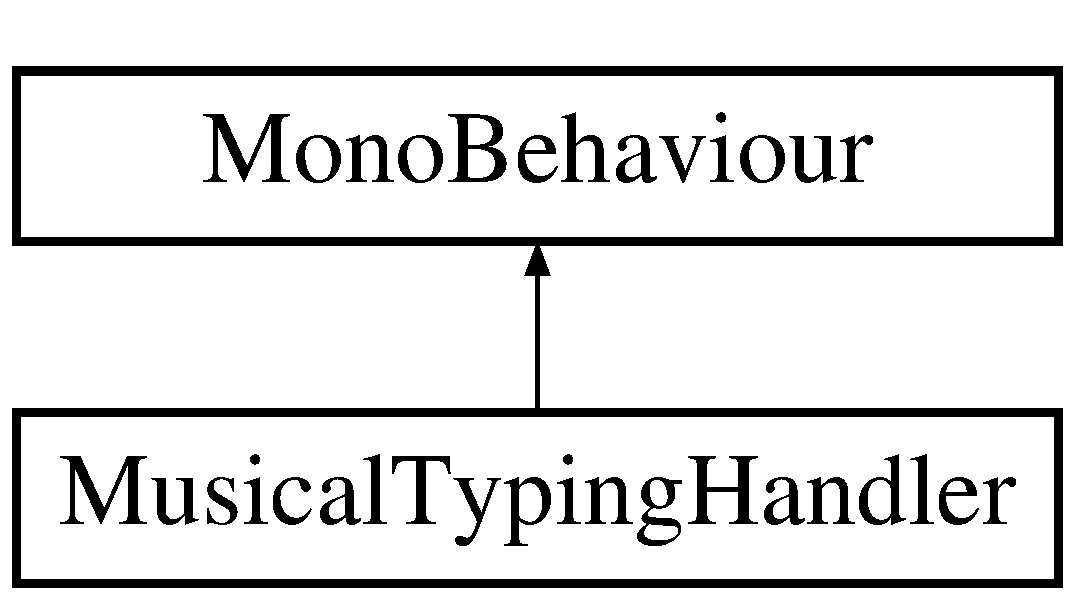
\includegraphics[height=2.000000cm]{class_musical_typing_handler}
\end{center}
\end{figure}
\subsection*{Public Member Functions}
\begin{DoxyCompactItemize}
\item 
void \hyperlink{group___mus_typ_pub_func_ga02f86b46bb63dc751b669035b7aa5ce0}{Set\+Key\+Velocity} (int a\+Key\+Index, int a\+Key\+Velocity)
\begin{DoxyCompactList}\small\item\em Sets the velocity used when a specific key on the computer keyboard generates a musical typing event. \end{DoxyCompactList}\item 
void \hyperlink{group___mus_typ_pub_func_gaf6ba35e3a081cff62fa963ed32d218c8}{Set\+Random\+Velocity\+Range} (int a\+Lowest\+Velocity, int a\+Highest\+Velocity)
\begin{DoxyCompactList}\small\item\em Sets the range used for randomizing Musical Typing velocities. \end{DoxyCompactList}\end{DoxyCompactItemize}
\subsection*{Public Attributes}
\begin{DoxyCompactItemize}
\item 
bool \hyperlink{group___mus_typ_pub_var_ga09a764161d537b31fac1a64ee5d39625}{Musical\+Typing\+Enabled} = true
\begin{DoxyCompactList}\small\item\em Is musical typing enabled? Default is true when the preprocessor flag is set. \end{DoxyCompactList}\item 
bool \hyperlink{group___mus_typ_pub_var_gad09f6f673034d9cd95f699838c9518d5}{Randomize\+Velocities} = false
\begin{DoxyCompactList}\small\item\em Should the velocities used for simulating a Note\+Play\+Event be randomized? Default is false. \end{DoxyCompactList}\end{DoxyCompactItemize}
\subsection*{Private Member Functions}
\begin{DoxyCompactItemize}
\item 
void \hyperlink{group___mus_typ_unity_ga2935e4d4209f57f19ea242968c861f3f}{Awake} ()
\begin{DoxyCompactList}\small\item\em Initializes the \hyperlink{class_musical_typing_handler}{Musical\+Typing\+Handler} by getting the parent \hyperlink{class_virtual_instrument_manager}{Virtual\+Instrument\+Manager} and calling Set\+Musical\+Typing\+Variables. \end{DoxyCompactList}\item 
void \hyperlink{group___mus_typ_unity_ga13a20522cf119917cb41e21051122977}{On\+G\+UI} ()
\begin{DoxyCompactList}\small\item\em Called whenever there is a G\+UI event. Used to see if the event is supposed to start a Musical Typing Event. \end{DoxyCompactList}\item 
void \hyperlink{group___mus_typ_priv_func_ga5db8ab750574dbc31279827ea5cc501e}{Set\+Musical\+Typing\+Variables} ()
\begin{DoxyCompactList}\small\item\em Sets the default values for musical typing. \end{DoxyCompactList}\item 
void \hyperlink{group___mus_typ_handlers_ga391a3d207136b7eb0e734e289b520188}{On\+Musical\+Typing\+Event} (Event a\+Key\+Event)
\begin{DoxyCompactList}\small\item\em Handler for Musical Typing Events. \end{DoxyCompactList}\end{DoxyCompactItemize}
\subsection*{Private Attributes}
\begin{DoxyCompactItemize}
\item 
\hyperlink{group___audio_testing_class_a_t_i___diagnostics}{A\+T\+I\+\_\+\+Diagnostics} \hyperlink{group___mus_typ_priv_var_gaaeabcb1c6445b0ff93059036cc4ec1f4}{m\+Diagnostics\+Handler} = null
\begin{DoxyCompactList}\small\item\em The handler for audio diagnostics display. \end{DoxyCompactList}\item 
bool \mbox{[}$\,$\mbox{]} \hyperlink{group___mus_typ_priv_var_gaede8bc4123f7bfe514816593fdfbec67}{m\+Pressed\+Keys} = null
\begin{DoxyCompactList}\small\item\em The keys that are currently pressed. \end{DoxyCompactList}\item 
int \mbox{[}$\,$\mbox{]} \hyperlink{group___mus_typ_priv_var_ga4836c9fe1805279497f421a29879bf5a}{m\+Key\+Velocities}
\begin{DoxyCompactList}\small\item\em The velocities that will be used whenever musical typing simulates a note event. \end{DoxyCompactList}\item 
int \mbox{[}$\,$\mbox{]} \hyperlink{group___mus_typ_priv_var_ga15df83911d88e77e46726ff5642d04e6}{m\+Random\+Velocity\+Range}
\begin{DoxyCompactList}\small\item\em The range used to randomize Musical Typing velocities. Default is 0 to 100. \end{DoxyCompactList}\item 
\hyperlink{class_virtual_instrument_manager}{Virtual\+Instrument\+Manager} \hyperlink{group___mus_typ_priv_var_ga63b2c5e1f9b1320a6b435a9018759444}{m\+V\+IM} = null
\begin{DoxyCompactList}\small\item\em The parent \hyperlink{class_virtual_instrument_manager}{Virtual\+Instrument\+Manager}. \end{DoxyCompactList}\end{DoxyCompactItemize}
\subsection*{Static Private Attributes}
\begin{DoxyCompactItemize}
\item 
static int \hyperlink{group___mus_typ_const_ga1a5182f5dda1cd3a5b400911a3f4cb69}{D\+E\+B\+U\+G\+\_\+num\+Musical\+Typing\+Keys} = 19
\begin{DoxyCompactList}\small\item\em The number of Musical Typing keys. \end{DoxyCompactList}\item 
static Key\+Code \mbox{[}$\,$\mbox{]} \hyperlink{group___mus_typ_const_gad8b9000a0b6c93d23310f54d07dd0b90}{D\+E\+B\+U\+G\+\_\+musical\+Typing\+Keys}
\begin{DoxyCompactList}\small\item\em The keys that are used for musical typing. \end{DoxyCompactList}\end{DoxyCompactItemize}


\subsection{Detailed Description}
Allows for testing the audio with the computer keyboard. 

Musical Typing allows for using a computer keyboard to debug sound output by triggering note events for a 19-\/note range whenever specific keys on the keyboard are pressed/released. The velocities for each key can be set with D\+E\+B\+U\+G\+\_\+\+Set\+Musical\+Typing\+Key\+Velocity(). The keys that are used are (in this order) a, w, s, e, d, f, t, g, y, h, u, j, k, o, l, p, ;, \textquotesingle{}, and \mbox{]} 

Definition at line 19 of file Musical\+Typing\+Handler.\+cs.



The documentation for this class was generated from the following file\+:\begin{DoxyCompactItemize}
\item 
D\+:/\+Documents/\+School Documents/2017\+Spring/\+E\+E\+C\+S542/\+V\+R\+Piano\+Project/\+Assets/\+Scripts/\+Audio/\+Testing/\hyperlink{_musical_typing_handler_8cs}{Musical\+Typing\+Handler.\+cs}\end{DoxyCompactItemize}

\hypertarget{class_note_output_object}{}\section{Note\+Output\+Object Class Reference}
\label{class_note_output_object}\index{Note\+Output\+Object@{Note\+Output\+Object}}


Unity Game\+Object that handles the actual output of sound.  


Inheritance diagram for Note\+Output\+Object\+:\begin{figure}[H]
\begin{center}
\leavevmode
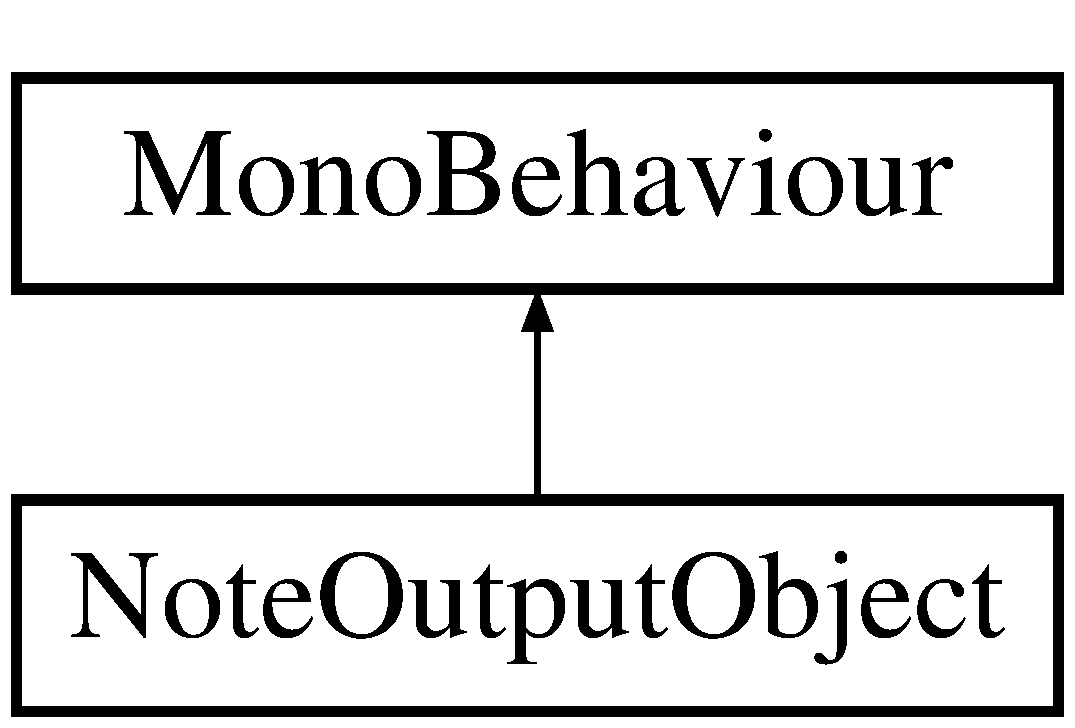
\includegraphics[height=2.000000cm]{class_note_output_object}
\end{center}
\end{figure}
\subsection*{Public Member Functions}
\begin{DoxyCompactItemize}
\item 
void \hyperlink{group___n_o_o_pub_func_ga2bdaa2787408f353f71ef6c6a18e9285}{Being\+Playing} (float a\+Velocity\+Factor, int a\+Dynamics\+Index, int a\+Start\+Index=0)
\begin{DoxyCompactList}\small\item\em Handler for setting the note to be played. Should be called from \hyperlink{group___v_i_m_event_types_class_virtual_instrument_manager_1_1_play_note_event}{the manager\textquotesingle{}s Play\+Note event}. \end{DoxyCompactList}\item 
void \hyperlink{group___n_o_o_pub_func_ga044e62759958d717c7fa4fd1615e2ec1}{Begin\+Release} ()
\begin{DoxyCompactList}\small\item\em Marks that the audio should begin fading out. \end{DoxyCompactList}\item 
bool \hyperlink{group___n_o_o_pub_func_ga24d76043802c442f571c5c34a854ff86}{Get\+Loop} ()
\begin{DoxyCompactList}\small\item\em Gets whether or not the audio should loop. \end{DoxyCompactList}\item 
void \hyperlink{group___n_o_o_pub_func_ga7977bc941f355866c7e4c141a8f7b8bb}{Pause\+Audio} ()
\begin{DoxyCompactList}\small\item\em Pauses the audio. \end{DoxyCompactList}\item 
void \hyperlink{group___n_o_o_pub_func_ga2df8edec357dd4123146c9a7e8485ffb}{Resume\+Audio} ()
\begin{DoxyCompactList}\small\item\em Resumes the audio. \end{DoxyCompactList}\item 
void \hyperlink{group___n_o_o_pub_func_gaef9ab691f0a2671a62249d853f24162d}{Set\+Audio\+Data} (float\mbox{[}$\,$\mbox{]}\mbox{[}$\,$\mbox{]} a\+Audio\+Data, Audio\+Mixer a\+Mixer, int\mbox{[}$\,$\mbox{]} a\+Thresholds=null)
\begin{DoxyCompactList}\small\item\em Sets the audio data for this object. \end{DoxyCompactList}\item 
void \hyperlink{group___n_o_o_pub_func_ga7b79bbd2c7a68831b322edff140f29d2}{Set\+Loop} (bool a\+Loop)
\begin{DoxyCompactList}\small\item\em Sets whether or not the audio should loop. \end{DoxyCompactList}\item 
void \hyperlink{group___n_o_o_pub_func_gaca261a6f8d95fc7f81bbc3c8108bad58}{Set\+V\+IM} (\hyperlink{class_virtual_instrument_manager}{Virtual\+Instrument\+Manager} a\+V\+IM)
\begin{DoxyCompactList}\small\item\em Sets the parent \hyperlink{class_virtual_instrument_manager}{Virtual\+Instrument\+Manager} and sets up diagnostics if needed. \end{DoxyCompactList}\item 
void \hyperlink{group___n_o_o_pub_func_gab7bad1b7d462676843be9e0bbfa1c9fb}{Should\+Notify\+When\+Finished} (bool a\+Should\+Notify)
\begin{DoxyCompactList}\small\item\em Sets whether or not an others should be notified when the audio has finished playing. \end{DoxyCompactList}\item 
void \hyperlink{group___n_o_o_pub_func_gae8a8e5bc027fd0186464a68399a4fecb}{Stop\+Audio} ()
\begin{DoxyCompactList}\small\item\em Stops playing the audio. \end{DoxyCompactList}\end{DoxyCompactItemize}
\subsection*{Private Member Functions}
\begin{DoxyCompactItemize}
\item 
void \hyperlink{group___n_o_o_unity_ga5c3cd343b7bfe7dec693d2cb69ec3cce}{Awake} ()
\begin{DoxyCompactList}\small\item\em Called when the object is created. This function creates an audio source and sets the initial values for each variable. \end{DoxyCompactList}\item 
void \hyperlink{group___n_o_o_priv_func_ga12f593bb5de83dc548eff4617fc687b5}{Remove\+Audio\+Data} ()
\begin{DoxyCompactList}\small\item\em Removes the audio data and resets relevant variables to default values. \end{DoxyCompactList}\item 
void \hyperlink{group___n_o_o_handlers_gaafd22f8a8c8d2cf101a54a4bf92782a5}{On\+Audio\+Filter\+Read} (float\mbox{[}$\,$\mbox{]} data, int channels)
\begin{DoxyCompactList}\small\item\em Handler that is called whenever the audio buffer is refilled. \end{DoxyCompactList}\end{DoxyCompactItemize}
\subsection*{Private Attributes}
\begin{DoxyCompactItemize}
\item 
\hyperlink{group___audio_testing_class_a_t_i___diagnostics}{A\+T\+I\+\_\+\+Diagnostics} \hyperlink{group___n_o_o_priv_var_gacd4376d2314caafc831cc049e9ca58d8}{m\+Diagnostics\+Handler} = null
\begin{DoxyCompactList}\small\item\em The audio diagnostics handler. \end{DoxyCompactList}\item 
Audio\+Source \hyperlink{group___n_o_o_priv_var_gad5e14a91b348e61166dbf6b6cf13649c}{m\+Source}
\begin{DoxyCompactList}\small\item\em The Audio\+Source component of this object. \end{DoxyCompactList}\item 
bool \hyperlink{group___n_o_o_priv_var_ga1efa96121f085b27c7d9e8725f90a336}{m\+Audio\+Data\+Being\+Used}
\begin{DoxyCompactList}\small\item\em Whether or not On\+Audio\+Filter\+Read is currently using the audio data. \end{DoxyCompactList}\item 
bool \hyperlink{group___n_o_o_priv_var_gaf01d2583555de6a523cdf82808718ca9}{m\+Loaded}
\begin{DoxyCompactList}\small\item\em Whether or not this object has loaded. \end{DoxyCompactList}\item 
bool \hyperlink{group___n_o_o_priv_var_gabf1d5013f44773e9fd3e4dbb59d74aeb}{m\+Loop}
\begin{DoxyCompactList}\small\item\em Whether or not the audio should loop. \end{DoxyCompactList}\item 
bool \hyperlink{group___n_o_o_priv_var_gac537ec036adf0645dca2f31fbc5b3dec}{m\+New\+Note}
\begin{DoxyCompactList}\small\item\em Whether or not a new note needs to be started. \end{DoxyCompactList}\item 
bool \hyperlink{group___n_o_o_priv_var_gaf72dd5943487433966b20b973be1e8b3}{m\+Notify\+When\+Finished}
\begin{DoxyCompactList}\small\item\em Should it notify the parent when the audio has finished playing? \end{DoxyCompactList}\item 
bool \hyperlink{group___n_o_o_priv_var_ga50fe6047e6a199215fc70b9fc78ac7eb}{m\+Paused}
\begin{DoxyCompactList}\small\item\em Is the audio paused? \end{DoxyCompactList}\item 
bool \hyperlink{group___n_o_o_priv_var_ga1f7a31f1aefc1633f1f435e3438a1efb}{m\+Resume}
\begin{DoxyCompactList}\small\item\em Whether or not the audio should resume from its previous position. \end{DoxyCompactList}\item 
bool \hyperlink{group___n_o_o_priv_var_ga4417170b8fa977f05a0b4cd0d16412fd}{m\+Note\+Playing}
\begin{DoxyCompactList}\small\item\em Whether or not the note is currently playing. \end{DoxyCompactList}\item 
bool \hyperlink{group___n_o_o_priv_var_ga88bfcc80d0cd20c81cd89d19d3231b84}{m\+Note\+Release}
\begin{DoxyCompactList}\small\item\em Whether or not the note has been released. \end{DoxyCompactList}\item 
bool \hyperlink{group___n_o_o_priv_var_gafa20525b5515ab62d109f44ab45fba21}{m\+Reported} = false
\begin{DoxyCompactList}\small\item\em Whether or not we have reported to the audio diagnostics handler. \end{DoxyCompactList}\item 
float \hyperlink{group___n_o_o_priv_var_gaf3cd650d21c56c25ce988d9f75279278}{m\+New\+Note\+Velocity\+Factor}
\begin{DoxyCompactList}\small\item\em The velocity of a new note mapped to the range \mbox{[}0,1\mbox{]}. \end{DoxyCompactList}\item 
float \hyperlink{group___n_o_o_priv_var_ga84df25e871d69746a7c520f3f8b49a27}{m\+Velocity\+Factor}
\begin{DoxyCompactList}\small\item\em A percentage mapping a given velocity to the output volume. \end{DoxyCompactList}\item 
float \mbox{[}$\,$\mbox{]}\mbox{[}$\,$\mbox{]} \hyperlink{group___n_o_o_priv_var_ga842eef5bfade070f914b8a551b3bcf43}{m\+Audio\+Data}
\begin{DoxyCompactList}\small\item\em A container for raw audio data. \end{DoxyCompactList}\item 
int \hyperlink{group___n_o_o_priv_var_ga5dca97be8d58837ace4ea6f4a972b20a}{m\+Counter}
\begin{DoxyCompactList}\small\item\em A counter to keep track of the current position in the raw audio data. \end{DoxyCompactList}\item 
int \hyperlink{group___n_o_o_priv_var_gaf0c9c2a90b5d73b8ffa0906bc69acdbc}{m\+Dynamics\+Index}
\begin{DoxyCompactList}\small\item\em The index corresponding to which built-\/in dynamics value is currently in use. \end{DoxyCompactList}\item 
int \hyperlink{group___n_o_o_priv_var_ga13de232048b35fc513f8aa3eeef65de0}{m\+New\+Note\+Dynamics\+Index}
\begin{DoxyCompactList}\small\item\em The dynamics index of the new note. \end{DoxyCompactList}\item 
int \hyperlink{group___n_o_o_priv_var_ga93720712088a4b6f91abe63d6f07a2c2}{m\+New\+Note\+Start\+Index}
\begin{DoxyCompactList}\small\item\em The index from which to start playing the audio. \end{DoxyCompactList}\item 
int \hyperlink{group___n_o_o_priv_var_ga3cc04564fcc1b1c4597af18e7e4fbc47}{m\+Num\+Built\+In\+Dynamics}
\begin{DoxyCompactList}\small\item\em The number of built-\/in dynamics values. \end{DoxyCompactList}\item 
int \mbox{[}$\,$\mbox{]} \hyperlink{group___n_o_o_priv_var_ga6a530f5e624caf8087c636df98d7f0b0}{m\+Built\+In\+Dynamics\+Thresholds}
\begin{DoxyCompactList}\small\item\em The thresholds that map a velocity to a built-\/in dynamics value. \end{DoxyCompactList}\item 
int \mbox{[}$\,$\mbox{]} \hyperlink{group___n_o_o_priv_var_ga48c676306790f40714072cd6a81a0128}{m\+End\+Sample\+Indices}
\begin{DoxyCompactList}\small\item\em The indices corresponding to the last sample in the audio data. \end{DoxyCompactList}\item 
\hyperlink{class_virtual_instrument_manager}{Virtual\+Instrument\+Manager} \hyperlink{group___n_o_o_priv_var_ga61394090fddcb90c67bf68f19a5bfb6e}{m\+V\+IM} = null
\begin{DoxyCompactList}\small\item\em The parent \hyperlink{class_virtual_instrument_manager}{Virtual\+Instrument\+Manager}. \end{DoxyCompactList}\end{DoxyCompactItemize}


\subsection{Detailed Description}
Unity Game\+Object that handles the actual output of sound. 

This class handles the sound output for \hyperlink{class_song}{Songs} and \hyperlink{group___v_i_m_event_types_class_virtual_instrument_manager_1_1_play_note_event}{Notes}. \hyperlink{group___v_i_m_priv_ga53f837fd01475fa35629a650e7fa00e3}{Copies of this object} are \hyperlink{group___v_i_m_priv_func_ga8817e32cc5074737b4d9489922b0fcb8}{dynamically created} by the \hyperlink{group___v_i_m}{Virtual Instrument Manager} for each \hyperlink{group___v_i_m_priv_ga5cedf9995d59b416412677e6004b659c}{note that can be played}. Separate copies are also created to \hyperlink{group___v_i_m_priv_gaa8d4f5642f5ac4dca4f4178b0052c78d}{handle playing Songs} and \hyperlink{group___v_i_m_priv_ga5f71cb71d240042312dcc13b481b068d}{drum loops}. ~\newline
 This class should only be handled by the \hyperlink{group___v_i_m}{Virtual Instrument Manager}. 

Definition at line 19 of file Note\+Output\+Object.\+cs.



The documentation for this class was generated from the following file\+:\begin{DoxyCompactItemize}
\item 
D\+:/\+Documents/\+School Documents/2017\+Spring/\+E\+E\+C\+S542/\+V\+R\+Piano\+Project/\+Assets/\+Scripts/\+Audio/\+Virtual\+Instrument/\hyperlink{_note_output_object_8cs}{Note\+Output\+Object.\+cs}\end{DoxyCompactItemize}

\hypertarget{class_piano}{}\section{Piano Class Reference}
\label{class_piano}\index{Piano@{Piano}}


A specific type of \hyperlink{group___v_i}{Virtual Instrument} that uses piano samples.  


Inheritance diagram for Piano\+:\begin{figure}[H]
\begin{center}
\leavevmode
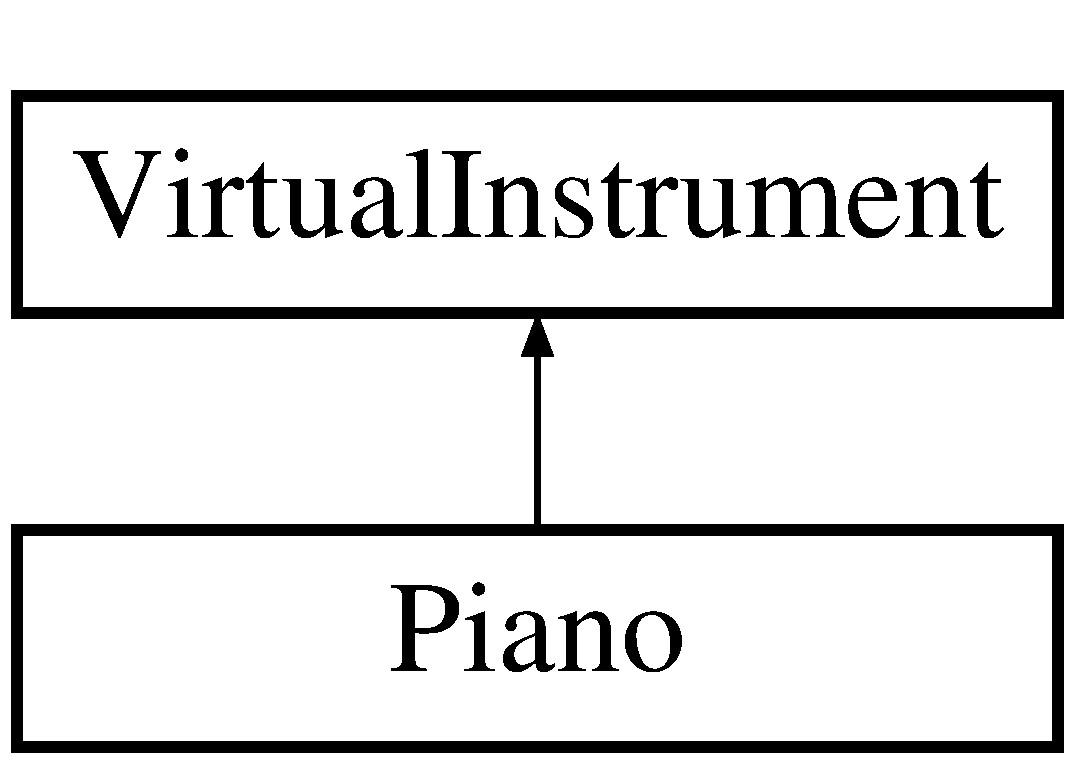
\includegraphics[height=2.000000cm]{class_piano}
\end{center}
\end{figure}
\subsection*{Public Member Functions}
\begin{DoxyCompactItemize}
\item 
\hyperlink{group___piano_construct_ga5128747ca1a1fbdc94a78362d3b87eed}{Piano} (\hyperlink{class_virtual_instrument_manager}{Virtual\+Instrument\+Manager} a\+Parent)
\begin{DoxyCompactList}\small\item\em Creates a new \hyperlink{class_piano}{Piano} instance. \end{DoxyCompactList}\end{DoxyCompactItemize}
\subsection*{Protected Member Functions}
\begin{DoxyCompactItemize}
\item 
override void \hyperlink{group___piano_virt_func_ga6bc02528f8808b8a30aa7d5776445a6d}{Initialize\+Built\+In\+Dynamics} ()
\begin{DoxyCompactList}\small\item\em Initializes values related to the \hyperlink{group___audio_DefBID}{Built-\/\+In Dynamics} for this instrument and allocates the audio data container. The \hyperlink{class_piano}{Piano} samples are available in three separate \hyperlink{group___audio_DefBID}{dynamics} \+: ~\newline
 pp\+: pianissimo (Very Soft) for \hyperlink{group___audio_DefVel}{velocities} from 0 to 50. ~\newline
 mf\+: mezzo-\/forte (Half-\/loud) for \hyperlink{group___audio_DefVel}{velocities} from 51 to 75. ~\newline
 ff\+: fortissimo (Very Loud) for \hyperlink{group___audio_DefVel}{velocities} from 76 to 100. \end{DoxyCompactList}\item 
override void \hyperlink{group___piano_virt_func_gaafd50f0f04ea7ea4f560accc628b8f1b}{Create\+Filenames} ()
\begin{DoxyCompactList}\small\item\em Creates the filenames from which to load the wav files. \end{DoxyCompactList}\end{DoxyCompactItemize}
\subsection*{Additional Inherited Members}


\subsection{Detailed Description}
A specific type of \hyperlink{group___v_i}{Virtual Instrument} that uses piano samples. 

The lowest \hyperlink{group___music_enums_ga508f69b199ea518f935486c990edac1d}{pitch} supported by the piano is \hyperlink{group___music_enums_ga508f69b199ea518f935486c990edac1d}{B0} and the highest \hyperlink{group___music_enums_ga508f69b199ea518f935486c990edac1d}{pitch} supported is \hyperlink{group___music_enums_ga508f69b199ea518f935486c990edac1d}{C8}.

~\newline
 This instrument is special (so far) in this project in that it supports \hyperlink{group___audio_DefBID}{Built-\/\+In Dynamics} with three different sound files for each pitch. Go to \hyperlink{group___audio_DefBID}{the section about Built-\/\+In Dynamics} for more details.

~\newline
 Its wav files are stored in \char`\"{}\+Resources/\+Audio/\+Virtual\+Instrument/\+Piano/\+Samples/ff\char`\"{}, \char`\"{}\+Resources/\+Audio/\+Virtual\+Instrument/\+Piano/\+Samples/mf\char`\"{}, and \char`\"{}\+Resources/\+Audio/\+Virtual\+Instrument/\+Piano/\+Samples/pp\char`\"{} 

Definition at line 31 of file Piano.\+cs.



The documentation for this class was generated from the following file\+:\begin{DoxyCompactItemize}
\item 
D\+:/\+Documents/\+School Documents/2017\+Spring/\+E\+E\+C\+S542/\+V\+R\+Piano\+Project/\+Assets/\+Scripts/\+Audio/\+Virtual\+Instrument/\hyperlink{_piano_8cs}{Piano.\+cs}\end{DoxyCompactItemize}

\hypertarget{class_s_c___load_song_dialog}{}\section{S\+C\+\_\+\+Load\+Song\+Dialog Class Reference}
\label{class_s_c___load_song_dialog}\index{S\+C\+\_\+\+Load\+Song\+Dialog@{S\+C\+\_\+\+Load\+Song\+Dialog}}


A dialog that loads a song into the \hyperlink{group___doc_s_c}{Song Creation Interface}.  


Inheritance diagram for S\+C\+\_\+\+Load\+Song\+Dialog\+:\begin{figure}[H]
\begin{center}
\leavevmode
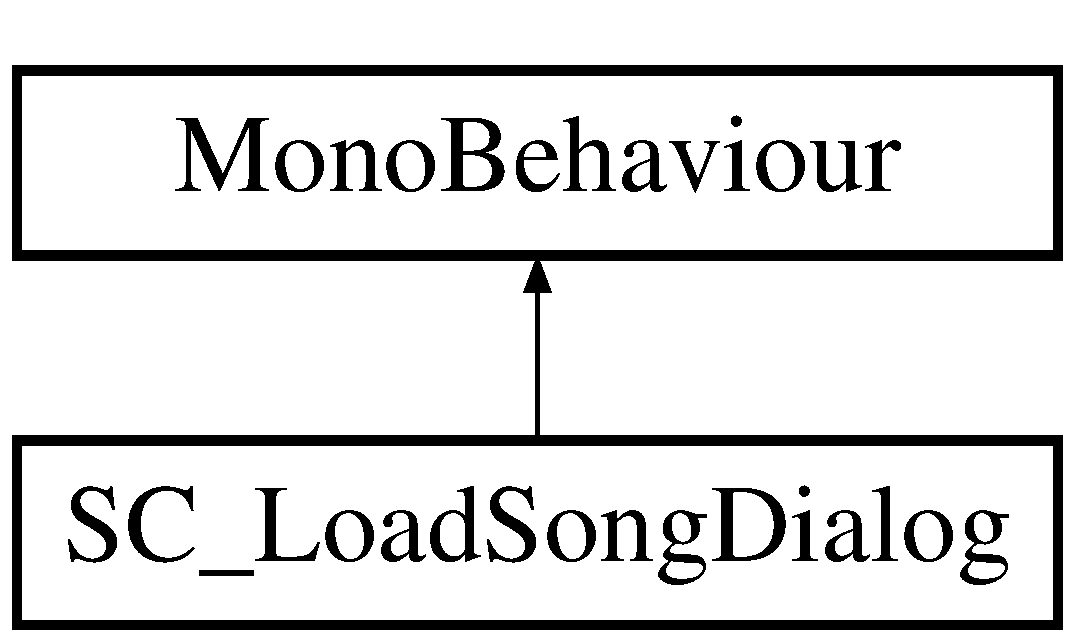
\includegraphics[height=2.000000cm]{class_s_c___load_song_dialog}
\end{center}
\end{figure}
\subsection*{Classes}
\begin{DoxyCompactItemize}
\item 
class \hyperlink{group___s_c___l_s_d_event_types_class_s_c___load_song_dialog_1_1_song_selected_event}{Song\+Selected\+Event}
\begin{DoxyCompactList}\small\item\em A type of event that is invoked when a song is selected to be loaded.  \hyperlink{group___s_c___l_s_d_event_types_class_s_c___load_song_dialog_1_1_song_selected_event}{More...}\end{DoxyCompactList}\end{DoxyCompactItemize}
\subsection*{Public Attributes}
\begin{DoxyCompactItemize}
\item 
\hyperlink{group___s_c___l_s_d_event_types_class_s_c___load_song_dialog_1_1_song_selected_event}{Song\+Selected\+Event} \hyperlink{group___s_c___l_s_d_events_ga48d606b2c8291fee822dcc2b14ddcecc}{Song\+Selected}
\begin{DoxyCompactList}\small\item\em The event that is invoked when a song is selected. No handler for this event in this class. It\textquotesingle{}s meant to notify other classes. \end{DoxyCompactList}\end{DoxyCompactItemize}
\subsection*{Private Member Functions}
\begin{DoxyCompactItemize}
\item 
void \hyperlink{group___s_c___l_s_d_unity_ga2fe8760877d7edd380795cac5749be50}{Awake} ()
\begin{DoxyCompactList}\small\item\em Initializes the \hyperlink{class_s_c___load_song_dialog}{S\+C\+\_\+\+Load\+Song\+Dialog} by getting references to its components. \end{DoxyCompactList}\item 
void \hyperlink{group___s_c___l_s_d_handlers_gacbe31698637339188fd50ba1a6723eab}{On\+Song\+Selected} (int a\+Index)
\begin{DoxyCompactList}\small\item\em Gets the selected \hyperlink{class_song}{Song} from the \hyperlink{class_song_manager_class}{song manager}. \end{DoxyCompactList}\item 
void \hyperlink{group___s_c___l_s_d_handlers_gae393a24bbdd4fa1d2b45fa4199fb453a}{On\+Cancel\+Button\+Clicked} ()
\begin{DoxyCompactList}\small\item\em Handles the \hyperlink{group___s_c___l_s_d_priv_var_ga31e17d7ca1cb32f0ad75ef8c7235873f}{Cancel button} being clicked with self-\/destruction. \end{DoxyCompactList}\item 
void \hyperlink{group___s_c___l_s_d_handlers_gad6ab852f2ac019395482e8c836061639}{On\+Load\+Button\+Clicked} ()
\begin{DoxyCompactList}\small\item\em Handles the \hyperlink{group___s_c___l_s_d_priv_var_gaa27cfb6231ef826024dd063828efa364}{Load button} being clicked by invoking the \hyperlink{group___s_c___l_s_d_event_types_class_s_c___load_song_dialog_1_1_song_selected_event}{Song\+Selected\+Event} and destroying itself. \end{DoxyCompactList}\end{DoxyCompactItemize}
\subsection*{Private Attributes}
\begin{DoxyCompactItemize}
\item 
Button \hyperlink{group___s_c___l_s_d_priv_var_ga31e17d7ca1cb32f0ad75ef8c7235873f}{m\+Cancel\+Button} = null
\begin{DoxyCompactList}\small\item\em The button to cancel loading a song. \end{DoxyCompactList}\item 
Button \hyperlink{group___s_c___l_s_d_priv_var_gaa27cfb6231ef826024dd063828efa364}{m\+Load\+Button} = null
\begin{DoxyCompactList}\small\item\em The button to load the selected song. \end{DoxyCompactList}\item 
Dropdown \hyperlink{group___s_c___l_s_d_priv_var_ga93543d4b5bf0c2127cb5489112cc29be}{m\+Song\+Selection\+Menu} = null
\begin{DoxyCompactList}\small\item\em The dropdown menu to select a song to load. \end{DoxyCompactList}\item 
\hyperlink{class_song}{Song} \hyperlink{group___s_c___l_s_d_priv_var_ga007db4c9493497f21fb518ab676226a4}{m\+Selected\+Song} = null
\begin{DoxyCompactList}\small\item\em The currently selected song. \end{DoxyCompactList}\item 
\hyperlink{class_virtual_instrument_manager}{Virtual\+Instrument\+Manager} \hyperlink{group___s_c___l_s_d_priv_var_ga6ffbaa999c431dd52e57c242b1b33b49}{m\+V\+IM} = null
\begin{DoxyCompactList}\small\item\em The \hyperlink{group___v_i_m}{Virtual Instrument Manager}. \end{DoxyCompactList}\end{DoxyCompactItemize}


\subsection{Detailed Description}
A dialog that loads a song into the \hyperlink{group___doc_s_c}{Song Creation Interface}. 

Definition at line 14 of file S\+C\+\_\+\+Load\+Song\+Dialog.\+cs.



The documentation for this class was generated from the following file\+:\begin{DoxyCompactItemize}
\item 
D\+:/\+Documents/\+School Documents/2017\+Spring/\+E\+E\+C\+S542/\+V\+R\+Piano\+Project/\+Assets/\+Scripts/\+Audio/\+Song\+Creation/\hyperlink{_s_c___load_song_dialog_8cs}{S\+C\+\_\+\+Load\+Song\+Dialog.\+cs}\end{DoxyCompactItemize}

\hypertarget{class_s_c___measure_display_panel}{}\section{S\+C\+\_\+\+Measure\+Display\+Panel Class Reference}
\label{class_s_c___measure_display_panel}\index{S\+C\+\_\+\+Measure\+Display\+Panel@{S\+C\+\_\+\+Measure\+Display\+Panel}}


Class that handles a specific measure of the \hyperlink{class_song}{Song} that is being created.  


Inheritance diagram for S\+C\+\_\+\+Measure\+Display\+Panel\+:\begin{figure}[H]
\begin{center}
\leavevmode
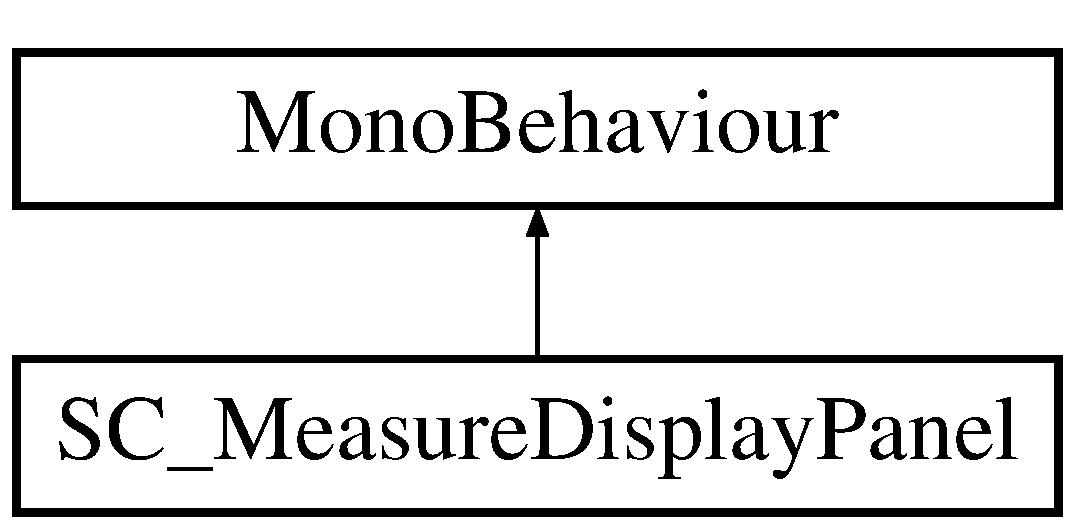
\includegraphics[height=2.000000cm]{class_s_c___measure_display_panel}
\end{center}
\end{figure}
\subsection*{Public Member Functions}
\begin{DoxyCompactItemize}
\item 
void \hyperlink{group___s_c___m_d_p_pub_func_gadce2fd2e70d867b38c98305e2392b3df}{Add\+Note} (int a\+Note\+Index, int a\+Melody\+Velocity, \hyperlink{group___music_enums_gaf11b5f079adbb21c800b9eca1c5c3cbd}{Music.\+N\+O\+T\+E\+\_\+\+L\+E\+N\+G\+TH} a\+Length, \hyperlink{group___music_enums_ga508f69b199ea518f935486c990edac1d}{Music.\+P\+I\+T\+CH}\mbox{[}$\,$\mbox{]} a\+Pitches, int a\+Drum\+Velocity, \hyperlink{group___music_enums_gade475b4382c7066d1af13e7c13c029b6}{Music.\+D\+R\+UM}\mbox{[}$\,$\mbox{]} a\+Drum\+Hits, \hyperlink{group___music_enums_gaf11b5f079adbb21c800b9eca1c5c3cbd}{Music.\+N\+O\+T\+E\+\_\+\+L\+E\+N\+G\+TH} a\+Offset\+From\+Prev\+Note)
\begin{DoxyCompactList}\small\item\em Adds a \hyperlink{group___music_structs_struct_music_1_1_combined_note}{note} to the \hyperlink{group___s_c___m_d_p_priv_var_gaf8a533bce87e58d8f7a1da88f476ac6f}{list of notes managed by this panel}. \end{DoxyCompactList}\item 
void \hyperlink{group___s_c___m_d_p_pub_func_ga5c4379bcb1309f70b7406eb6523c6179}{Clear\+Measure} ()
\begin{DoxyCompactList}\small\item\em Clears the notes in the measure and self-\/destructs. \end{DoxyCompactList}\item 
void \hyperlink{group___s_c___m_d_p_pub_func_ga334c177603c25d6206b7c7b639281b07}{Set\+Parent\+Container} (\hyperlink{class_s_c___note_display_container}{S\+C\+\_\+\+Note\+Display\+Container} a\+Parent)
\begin{DoxyCompactList}\small\item\em Sets the \hyperlink{group___doc_s_c___n_d_c}{parent container}. \end{DoxyCompactList}\item 
void \hyperlink{group___s_c___m_d_p_pub_func_gab8a32b1ba282d441cb1325d29f53dd1c}{Set\+Percentage\+Used} (float a\+Percent)
\begin{DoxyCompactList}\small\item\em Sets the percentage of the measure that is filled. \end{DoxyCompactList}\item 
void \hyperlink{group___s_c___m_d_p_pub_func_ga6512fa5010bcecd85f7e8542cea91310}{Set\+Toggle} (bool a\+Show\+Measure)
\begin{DoxyCompactList}\small\item\em Sets whether or not the measure should be shown. \end{DoxyCompactList}\item 
void \hyperlink{group___s_c___m_d_p_handlers_ga31c72fee5ddd5ae7b057b2f265341263}{On\+Show\+Toggle} (bool a\+Show\+Measure)
\begin{DoxyCompactList}\small\item\em Handles showing the measure or hiding it. \end{DoxyCompactList}\item 
void \hyperlink{group___s_c___m_d_p_handlers_gab48fa7fe4d7d4b29a3b0567be2b29849}{On\+Remove\+Note} (\hyperlink{class_s_c___note_display_panel}{S\+C\+\_\+\+Note\+Display\+Panel} a\+Note\+Display\+Panel)
\begin{DoxyCompactList}\small\item\em Removes a \hyperlink{group___music_structs_struct_music_1_1_combined_note}{note}. \end{DoxyCompactList}\end{DoxyCompactItemize}
\subsection*{Private Member Functions}
\begin{DoxyCompactItemize}
\item 
void \hyperlink{group___s_c___m_d_p_unity_gafe9062b7be241c5febf7b493bb6002f9}{Awake} ()
\begin{DoxyCompactList}\small\item\em Initializes the \hyperlink{class_s_c___measure_display_panel}{S\+C\+\_\+\+Measure\+Display\+Panel}. \end{DoxyCompactList}\end{DoxyCompactItemize}
\subsection*{Private Attributes}
\begin{DoxyCompactItemize}
\item 
string \hyperlink{group___s_c___m_d_p_const_ga6eee69b23fe2146403f41e4e862a3df9}{N\+O\+T\+E\+\_\+\+D\+I\+S\+P\+L\+A\+Y\+\_\+\+P\+A\+N\+E\+L\+\_\+\+P\+A\+TH} = \char`\"{}Audio/Prefabs/Song\+Creation/Note\+Display\+Panel\+Prefab\char`\"{}
\begin{DoxyCompactList}\small\item\em The path to load the \hyperlink{group___doc_s_c___n_d_p}{S\+C\+\_\+\+Note\+Display\+Panel}\textquotesingle{}s prefab. \end{DoxyCompactList}\item 
float \hyperlink{group___s_c___m_d_p_priv_var_ga7567e9001016a06d950b9d0cc9e1d905}{m\+Percentage\+Used} = 0f
\begin{DoxyCompactList}\small\item\em The percentage of the measure used. \end{DoxyCompactList}\item 
List$<$ \hyperlink{class_s_c___note_display_panel}{S\+C\+\_\+\+Note\+Display\+Panel} $>$ \hyperlink{group___s_c___m_d_p_priv_var_gaf8a533bce87e58d8f7a1da88f476ac6f}{m\+Notes} = null
\begin{DoxyCompactList}\small\item\em The notes in the measure. \end{DoxyCompactList}\item 
\hyperlink{class_s_c___note_display_container}{S\+C\+\_\+\+Note\+Display\+Container} \hyperlink{group___s_c___m_d_p_priv_var_ga6f22ae359dd68605a8b2fd961ced96b5}{m\+Parent} = null
\begin{DoxyCompactList}\small\item\em The parent container. \end{DoxyCompactList}\item 
Toggle \hyperlink{group___s_c___m_d_p_priv_var_gabec551ab0b79d269b028f4bc99e82b00}{m\+Show\+Measure\+Toggle} = null
\begin{DoxyCompactList}\small\item\em The toggle switch for showing this measure. \end{DoxyCompactList}\end{DoxyCompactItemize}


\subsection{Detailed Description}
Class that handles a specific measure of the \hyperlink{class_song}{Song} that is being created. 

This class allows for showing specific measures of the \hyperlink{class_song}{Song} at a time in order to cut down on clutter. 

Definition at line 18 of file S\+C\+\_\+\+Measure\+Display\+Panel.\+cs.



The documentation for this class was generated from the following file\+:\begin{DoxyCompactItemize}
\item 
D\+:/\+Documents/\+School Documents/2017\+Spring/\+E\+E\+C\+S542/\+V\+R\+Piano\+Project/\+Assets/\+Scripts/\+Audio/\+Song\+Creation/\hyperlink{_s_c___measure_display_panel_8cs}{S\+C\+\_\+\+Measure\+Display\+Panel.\+cs}\end{DoxyCompactItemize}

\hypertarget{class_s_c___note_display_container}{}\section{S\+C\+\_\+\+Note\+Display\+Container Class Reference}
\label{class_s_c___note_display_container}\index{S\+C\+\_\+\+Note\+Display\+Container@{S\+C\+\_\+\+Note\+Display\+Container}}


Connects the \hyperlink{class_s_c___measure_display_panel}{S\+C\+\_\+\+Measure\+Display\+Panel} objects to the \hyperlink{group___doc_s_c}{Song Creation Interface} and provides handling for them.  


Inheritance diagram for S\+C\+\_\+\+Note\+Display\+Container\+:\begin{figure}[H]
\begin{center}
\leavevmode
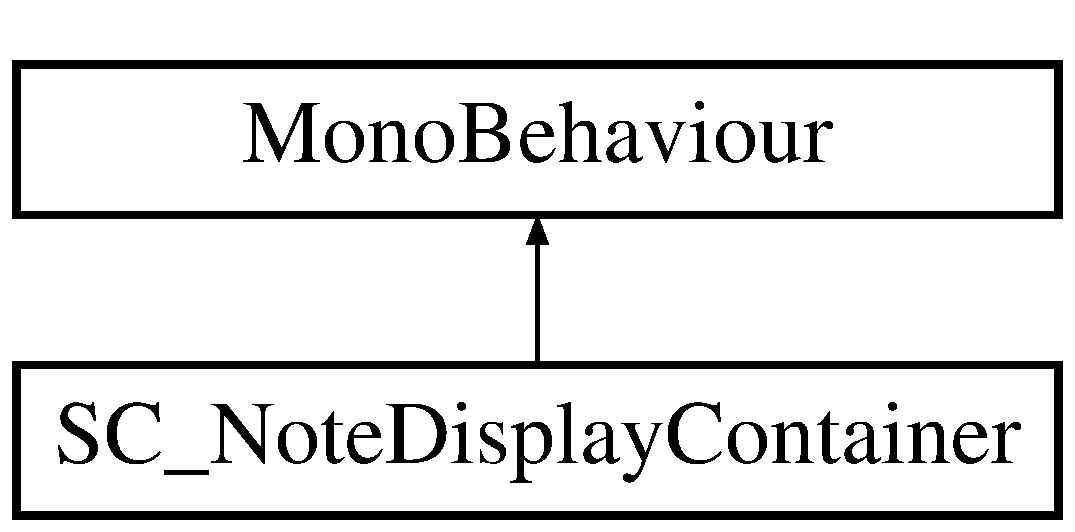
\includegraphics[height=2.000000cm]{class_s_c___note_display_container}
\end{center}
\end{figure}
\subsection*{Public Member Functions}
\begin{DoxyCompactItemize}
\item 
void \hyperlink{group___s_c___n_d_c_pub_func_ga43e58800daae0e46bbe1b86d78c2f677}{Add\+Note} (int a\+Melody\+Velocity, \hyperlink{group___music_enums_gaf11b5f079adbb21c800b9eca1c5c3cbd}{Music.\+N\+O\+T\+E\+\_\+\+L\+E\+N\+G\+TH} a\+Length, \hyperlink{group___music_enums_ga508f69b199ea518f935486c990edac1d}{Music.\+P\+I\+T\+CH}\mbox{[}$\,$\mbox{]} a\+Pitches, int a\+Drum\+Velocity, \hyperlink{group___music_enums_gade475b4382c7066d1af13e7c13c029b6}{Music.\+D\+R\+UM}\mbox{[}$\,$\mbox{]} a\+Drum\+Hits, \hyperlink{group___music_enums_gaf11b5f079adbb21c800b9eca1c5c3cbd}{Music.\+N\+O\+T\+E\+\_\+\+L\+E\+N\+G\+TH} a\+Offset\+From\+Prev\+Note)
\begin{DoxyCompactList}\small\item\em Adds a \hyperlink{group___music_structs_struct_music_1_1_combined_note}{note} to the \hyperlink{group___doc_s_c___m_d_p}{current measure}. \end{DoxyCompactList}\item 
void \hyperlink{group___s_c___n_d_c_pub_func_gaa344983500e83531210ae1c4789182f3}{Clear\+Notes} ()
\begin{DoxyCompactList}\small\item\em Clears all of the notes. \end{DoxyCompactList}\item 
\hyperlink{class_s_c___measure_display_panel}{S\+C\+\_\+\+Measure\+Display\+Panel} \hyperlink{group___s_c___n_d_c_pub_func_ga526a610a4462b164cc91ae7155803ba1}{Get\+Current\+Measure\+Object} ()
\begin{DoxyCompactList}\small\item\em Gets the current \hyperlink{group___doc_s_c___m_d_p}{measure}. \end{DoxyCompactList}\item 
Sprite \mbox{[}$\,$\mbox{]} \hyperlink{group___s_c___n_d_c_pub_func_ga3cdbb1068cd6511112c564fc636c56ca}{Get\+Sprites} ()
\begin{DoxyCompactList}\small\item\em Gets the images used to represent a note\textquotesingle{}s \hyperlink{group___music_structs_ac35cd02f5b3c00e3040b51e40e9e6c94}{length}/\hyperlink{group___music_structs_ae281187907aed4c728c7981300dbebaf}{offset}. \end{DoxyCompactList}\item 
void \hyperlink{group___s_c___n_d_c_handlers_ga40c5a3b59608c559ab96ad0338c5e042}{Handle\+Full\+Measure} (\hyperlink{class_s_c___measure_display_panel}{S\+C\+\_\+\+Measure\+Display\+Panel} a\+Full\+Measure, float a\+Spillover, int a\+Melody\+Velocity, \hyperlink{group___music_enums_gaf11b5f079adbb21c800b9eca1c5c3cbd}{Music.\+N\+O\+T\+E\+\_\+\+L\+E\+N\+G\+TH} a\+Length, \hyperlink{group___music_enums_ga508f69b199ea518f935486c990edac1d}{Music.\+P\+I\+T\+CH}\mbox{[}$\,$\mbox{]} a\+Pitches, int a\+Drum\+Velocity, \hyperlink{group___music_enums_gade475b4382c7066d1af13e7c13c029b6}{Music.\+D\+R\+UM}\mbox{[}$\,$\mbox{]} a\+Drum\+Hits, \hyperlink{group___music_enums_gaf11b5f079adbb21c800b9eca1c5c3cbd}{Music.\+N\+O\+T\+E\+\_\+\+L\+E\+N\+G\+TH} a\+Offset\+From\+Prev\+Note)
\begin{DoxyCompactList}\small\item\em Handler for when a \hyperlink{group___doc_s_c___m_d_p}{measure} fills up. \end{DoxyCompactList}\item 
void \hyperlink{group___s_c___n_d_c_handlers_ga40ffb2c779af43930924348c265c9e09}{Handle\+Measure\+Deleted} (\hyperlink{class_s_c___measure_display_panel}{S\+C\+\_\+\+Measure\+Display\+Panel} a\+Measure)
\begin{DoxyCompactList}\small\item\em Handles when a \hyperlink{group___doc_s_c___m_d_p}{measure} has all of its \hyperlink{group___music_structs_struct_music_1_1_combined_note}{notes} removed by deleting the \hyperlink{group___doc_s_c___m_d_p}{measure object}. \end{DoxyCompactList}\item 
void \hyperlink{group___s_c___n_d_c_handlers_ga458d57203645be514d3626211044b584}{Handle\+Measure\+Toggled} (\hyperlink{class_s_c___measure_display_panel}{S\+C\+\_\+\+Measure\+Display\+Panel} a\+Measure)
\begin{DoxyCompactList}\small\item\em Handles when a \hyperlink{group___doc_s_c___m_d_p}{measure} is \hyperlink{group___s_c___m_d_p_handlers_ga31c72fee5ddd5ae7b057b2f265341263}{toggled}. \end{DoxyCompactList}\item 
void \hyperlink{group___s_c___n_d_c_handlers_ga6dbbf12e55681d13f43e489dd4a100dc}{On\+Remove\+Note} ()
\begin{DoxyCompactList}\small\item\em Handles when a note is removed by decreasing the count of notes in the song. \end{DoxyCompactList}\end{DoxyCompactItemize}
\subsection*{Private Member Functions}
\begin{DoxyCompactItemize}
\item 
void \hyperlink{group___s_c___n_d_c_unity_ga6ce4069508f84edd9e13d8fab4c26e09}{Awake} ()
\begin{DoxyCompactList}\small\item\em Initializes the \hyperlink{class_s_c___note_display_container}{S\+C\+\_\+\+Note\+Display\+Container}. \end{DoxyCompactList}\end{DoxyCompactItemize}
\subsection*{Private Attributes}
\begin{DoxyCompactItemize}
\item 
const string \hyperlink{group___s_c___n_d_c_const_gabc95cd739b62996e8a19f0e9417e5f8e}{M\+E\+A\+S\+U\+R\+E\+\_\+\+P\+A\+N\+E\+L\+\_\+\+P\+R\+E\+F\+A\+B\+\_\+\+P\+A\+TH} = \char`\"{}Audio/Prefabs/Song\+Creation/Measure\+Panel\+Prefab\char`\"{}
\begin{DoxyCompactList}\small\item\em The path to load the prefab for the \hyperlink{group___doc_s_c___m_d_p}{measure display panel objects}. \end{DoxyCompactList}\item 
int \hyperlink{group___s_c___n_d_c_priv_var_gae06a4919a63806ed57b2040f41b7ca1b}{m\+Num\+Notes} = 0
\begin{DoxyCompactList}\small\item\em The number of overall \hyperlink{group___music_structs_struct_music_1_1_combined_note}{notes} in the container. \end{DoxyCompactList}\item 
int \hyperlink{group___s_c___n_d_c_priv_var_ga28ce2bf8358c9f686b5b9e362aa96dff}{m\+Current\+Measure} = -\/1
\begin{DoxyCompactList}\small\item\em The current \hyperlink{group___doc_s_c___m_d_p}{measure}. \end{DoxyCompactList}\item 
List$<$ \hyperlink{class_s_c___measure_display_panel}{S\+C\+\_\+\+Measure\+Display\+Panel} $>$ \hyperlink{group___s_c___n_d_c_priv_var_gaa072fb53f6bd6646bc85f2ebc2a02229}{m\+Measures} = null
\begin{DoxyCompactList}\small\item\em The \hyperlink{group___doc_s_c___m_d_p}{measures} in the container. \end{DoxyCompactList}\item 
Sprite \mbox{[}$\,$\mbox{]} \hyperlink{group___s_c___n_d_c_priv_var_gac8df613ee0996e999278da2b3f523e34}{m\+Sprites} = null
\begin{DoxyCompactList}\small\item\em The images to show the \hyperlink{group___music_structs_ac35cd02f5b3c00e3040b51e40e9e6c94}{note lengths} and \hyperlink{group___music_structs_ae281187907aed4c728c7981300dbebaf}{offsets}. \end{DoxyCompactList}\end{DoxyCompactItemize}


\subsection{Detailed Description}
Connects the \hyperlink{class_s_c___measure_display_panel}{S\+C\+\_\+\+Measure\+Display\+Panel} objects to the \hyperlink{group___doc_s_c}{Song Creation Interface} and provides handling for them. 

Definition at line 13 of file S\+C\+\_\+\+Note\+Display\+Container.\+cs.



The documentation for this class was generated from the following file\+:\begin{DoxyCompactItemize}
\item 
D\+:/\+Documents/\+School Documents/2017\+Spring/\+E\+E\+C\+S542/\+V\+R\+Piano\+Project/\+Assets/\+Scripts/\+Audio/\+Song\+Creation/\hyperlink{_s_c___note_display_container_8cs}{S\+C\+\_\+\+Note\+Display\+Container.\+cs}\end{DoxyCompactItemize}

\hypertarget{class_s_c___note_display_panel}{}\section{S\+C\+\_\+\+Note\+Display\+Panel Class Reference}
\label{class_s_c___note_display_panel}\index{S\+C\+\_\+\+Note\+Display\+Panel@{S\+C\+\_\+\+Note\+Display\+Panel}}


Class that displays a specific \hyperlink{group___music_structs_struct_music_1_1_combined_note}{note} of the \hyperlink{class_song}{Song} that is being created.  


Inheritance diagram for S\+C\+\_\+\+Note\+Display\+Panel\+:\begin{figure}[H]
\begin{center}
\leavevmode
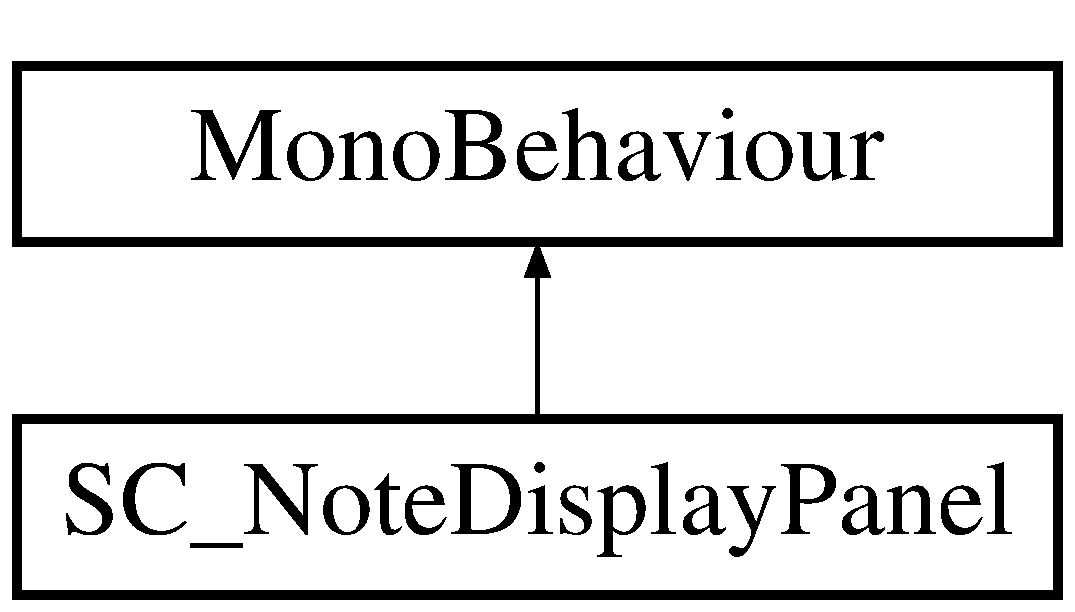
\includegraphics[height=2.000000cm]{class_s_c___note_display_panel}
\end{center}
\end{figure}
\subsection*{Public Member Functions}
\begin{DoxyCompactItemize}
\item 
Sprite \hyperlink{group___s_c___n_d_p_unity_ga1038892636ae54a79c675287c4bb6fff}{Get\+Length\+Image} ()
\begin{DoxyCompactList}\small\item\em Gets the image used to represent the length of the note. \end{DoxyCompactList}\item 
\hyperlink{class_s_c___measure_display_panel}{S\+C\+\_\+\+Measure\+Display\+Panel} \hyperlink{group___s_c___n_d_p_unity_ga404972fc48a89d678d0c6fa801573814}{Get\+Measure\+Panel} ()
\begin{DoxyCompactList}\small\item\em Gets the measure panel that is managing this panel. \end{DoxyCompactList}\item 
int \hyperlink{group___s_c___n_d_p_unity_ga8beef050026ade4ba4ccb574c414d24e}{Get\+Note\+Index} ()
\begin{DoxyCompactList}\small\item\em Gets the index for this note. \end{DoxyCompactList}\item 
\hyperlink{group___music_enums_gaf11b5f079adbb21c800b9eca1c5c3cbd}{Music.\+N\+O\+T\+E\+\_\+\+L\+E\+N\+G\+TH} \hyperlink{group___s_c___n_d_p_unity_ga371654221730812200062322c8a3e750}{Get\+Offset} ()
\begin{DoxyCompactList}\small\item\em Gets the offset of this note. \end{DoxyCompactList}\item 
void \hyperlink{group___s_c___n_d_p_unity_gae14b5564be204df7699b95186d83f69f}{Set\+Drums} (string a\+Drum\+String)
\begin{DoxyCompactList}\small\item\em Sets the drum string for the note. \end{DoxyCompactList}\item 
void \hyperlink{group___s_c___n_d_p_unity_ga1a1c4b8111463ec3e134d17fe5064a54}{Set\+Length\+Image} (Sprite a\+Image)
\begin{DoxyCompactList}\small\item\em Sets the image used to represent the \hyperlink{group___music_enums_gaf11b5f079adbb21c800b9eca1c5c3cbd}{length} of the \hyperlink{group___music_structs_struct_music_1_1_combined_note}{note}. \end{DoxyCompactList}\item 
void \hyperlink{group___s_c___n_d_p_unity_ga8ff7588e8c3f59a03842feaff92f97e9}{Set\+Offset} (\hyperlink{group___music_enums_gaf11b5f079adbb21c800b9eca1c5c3cbd}{Music.\+N\+O\+T\+E\+\_\+\+L\+E\+N\+G\+TH} a\+Offset)
\begin{DoxyCompactList}\small\item\em Sets the \hyperlink{group___music_structs_ae281187907aed4c728c7981300dbebaf}{offset} of the \hyperlink{group___music_structs_struct_music_1_1_combined_note}{note} being displayed. \end{DoxyCompactList}\item 
void \hyperlink{group___s_c___n_d_p_unity_gaa0a517d1359cd1ed109a130bd52763f1}{Set\+Offset\+Image} (Sprite a\+Image)
\begin{DoxyCompactList}\small\item\em Sets the image used to represent the \hyperlink{group___music_structs_ae281187907aed4c728c7981300dbebaf}{offset} of the \hyperlink{group___music_structs_struct_music_1_1_combined_note}{note} being displayed. \end{DoxyCompactList}\item 
void \hyperlink{group___s_c___n_d_p_unity_gae642b50484b9c7fb2bd3b201aeef726c}{Set\+Parent\+Container} (\hyperlink{class_s_c___measure_display_panel}{S\+C\+\_\+\+Measure\+Display\+Panel} a\+Parent)
\begin{DoxyCompactList}\small\item\em Sets the \hyperlink{group___doc_s_c___m_d_p}{parent container}. \end{DoxyCompactList}\item 
void \hyperlink{group___s_c___n_d_p_unity_gaf3160e3686e44e7718768242438ea1cc}{Set\+Note\+Index} (int a\+Index)
\begin{DoxyCompactList}\small\item\em Sets the index for this \hyperlink{group___music_structs_struct_music_1_1_combined_note}{note} in the \hyperlink{class_song}{Song}. \end{DoxyCompactList}\item 
void \hyperlink{group___s_c___n_d_p_unity_gad9bf776f0c51cf6170faccf9fc4ac7e0}{Set\+Pitches} (string a\+Pitch\+String)
\begin{DoxyCompactList}\small\item\em Sets the string that represents the \hyperlink{group___music_enums_ga508f69b199ea518f935486c990edac1d}{pitches} in the \hyperlink{group___music_structs_struct_music_1_1_combined_note}{note} being displayed. \end{DoxyCompactList}\item 
void \hyperlink{group___s_c___n_d_p_unity_ga8a2fef715606caa884c7b490850fb9b7}{Set\+Velocity} (string a\+Velocity\+String)
\item 
void \hyperlink{group___s_c___n_d_p_unity_ga92d0f078c4efd6c207173a10e31b5065}{Stop\+Editing} ()
\begin{DoxyCompactList}\small\item\em Sets that we\textquotesingle{}re no longer editing the note that this panel represents. \end{DoxyCompactList}\item 
void \hyperlink{group___s_c___n_d_p_handlers_ga0b545f6cd12ce56258842cb1036bceec}{On\+Remove\+Button\+Clicked} ()
\begin{DoxyCompactList}\small\item\em Handles when the \hyperlink{group___s_c___n_d_p_priv_var_gac9af0bdc5b04a52ab9e7c13a0ad01ab7}{remove button} is clicked. \end{DoxyCompactList}\end{DoxyCompactItemize}
\subsection*{Private Member Functions}
\begin{DoxyCompactItemize}
\item 
void \hyperlink{group___s_c___n_d_p_unity_ga131f594d4f9b5887acb0de0a8bb5532a}{Awake} ()
\begin{DoxyCompactList}\small\item\em Initializes the \hyperlink{class_s_c___note_display_panel}{S\+C\+\_\+\+Note\+Display\+Panel} by getting references to its child objects and adding event handlers. \end{DoxyCompactList}\item 
void \hyperlink{group___s_c___n_d_p_handlers_ga7b25bcc6b76ae0894ac6eefde417caf1}{Trigger\+Edit\+Event} (Pointer\+Event\+Data a\+Pointer\+Data)
\begin{DoxyCompactList}\small\item\em Handles clicking on the background panel which means that we\textquotesingle{}re either beginning an edit to this \hyperlink{group___music_structs_struct_music_1_1_combined_note}{note} or cancelling it. \end{DoxyCompactList}\end{DoxyCompactItemize}
\subsection*{Private Attributes}
\begin{DoxyCompactItemize}
\item 
Button \hyperlink{group___s_c___n_d_p_priv_var_gac9af0bdc5b04a52ab9e7c13a0ad01ab7}{m\+Remove\+Note\+Button} = null
\begin{DoxyCompactList}\small\item\em The button to remove this note. \end{DoxyCompactList}\item 
Event\+Trigger \hyperlink{group___s_c___n_d_p_priv_var_ga3dd3e8ce9fbbe9b6b11d87e28df7dcfa}{m\+Edit\+Trigger} = null
\begin{DoxyCompactList}\small\item\em The edit trigger. \end{DoxyCompactList}\item 
Image \hyperlink{group___s_c___n_d_p_priv_var_ga611f26eaf6a960570b0dd848b6712b5f}{m\+Length\+Image} = null
\begin{DoxyCompactList}\small\item\em The image to show the note\textquotesingle{}s length. \end{DoxyCompactList}\item 
Image \hyperlink{group___s_c___n_d_p_priv_var_ga177d14cf2cac316a0bfc2e1096256a0c}{m\+Offset\+Image} = null
\begin{DoxyCompactList}\small\item\em The image to show the note\textquotesingle{}s offset from the previous note. \end{DoxyCompactList}\item 
int \hyperlink{group___s_c___n_d_p_priv_var_ga11933919195aba904a4e8bf95f131e49}{m\+Note\+Index} = 0
\begin{DoxyCompactList}\small\item\em The inde of this note. \end{DoxyCompactList}\item 
\hyperlink{class_s_c___measure_display_panel}{S\+C\+\_\+\+Measure\+Display\+Panel} \hyperlink{group___s_c___n_d_p_priv_var_ga360017747d9ed8910ddd4b3309477710}{m\+Parent} = null
\begin{DoxyCompactList}\small\item\em The parent container. \end{DoxyCompactList}\item 
\hyperlink{group___music_enums_gaf11b5f079adbb21c800b9eca1c5c3cbd}{Music.\+N\+O\+T\+E\+\_\+\+L\+E\+N\+G\+TH} \hyperlink{group___s_c___n_d_p_priv_var_ga0a78a2c25da29d944d56d1c8ebb74d03}{m\+Offset} = \hyperlink{group___music_enums_ggaf11b5f079adbb21c800b9eca1c5c3cbdab50339a10e1de285ac99d4c3990b8693}{Music.\+N\+O\+T\+E\+\_\+\+L\+E\+N\+G\+T\+H.\+N\+O\+NE}
\begin{DoxyCompactList}\small\item\em The offset. \end{DoxyCompactList}\item 
\hyperlink{class_song_creation_manager}{Song\+Creation\+Manager} \hyperlink{group___s_c___n_d_p_priv_var_ga5e4ae5e7daa568c3e2b471c0835600c6}{m\+Song\+Creation\+Handler} = null
\begin{DoxyCompactList}\small\item\em The song creation scene handler. \end{DoxyCompactList}\item 
Text \hyperlink{group___s_c___n_d_p_priv_var_gadd38ff2acddedee4b6165f2fc48fd43c}{m\+Drums} = null
\begin{DoxyCompactList}\small\item\em The text that displays the note\textquotesingle{}s drums. \end{DoxyCompactList}\item 
Text \hyperlink{group___s_c___n_d_p_priv_var_ga8018aa4f7b333a7129badf082f233a3c}{m\+Pitches} = null
\begin{DoxyCompactList}\small\item\em The text that displays the note\textquotesingle{}s pitches. \end{DoxyCompactList}\item 
Text \hyperlink{group___s_c___n_d_p_priv_var_ga4924aa3f63f171ed33f5f85d11a760c4}{m\+Velocity} = null
\begin{DoxyCompactList}\small\item\em The text that displays the note\textquotesingle{}s velocity. \end{DoxyCompactList}\end{DoxyCompactItemize}


\subsection{Detailed Description}
Class that displays a specific \hyperlink{group___music_structs_struct_music_1_1_combined_note}{note} of the \hyperlink{class_song}{Song} that is being created. 

This class is held in the \hyperlink{group___doc_s_c___n_d_c}{Note Display Container} and managed by the \hyperlink{group___doc_s_c___m_d_p}{measure display panel}. 

Definition at line 19 of file S\+C\+\_\+\+Note\+Display\+Panel.\+cs.



The documentation for this class was generated from the following file\+:\begin{DoxyCompactItemize}
\item 
D\+:/\+Documents/\+School Documents/2017\+Spring/\+E\+E\+C\+S542/\+V\+R\+Piano\+Project/\+Assets/\+Scripts/\+Audio/\+Song\+Creation/\hyperlink{_s_c___note_display_panel_8cs}{S\+C\+\_\+\+Note\+Display\+Panel.\+cs}\end{DoxyCompactItemize}

\hypertarget{class_s_c___pitch_selection_container}{}\section{S\+C\+\_\+\+Pitch\+Selection\+Container Class Reference}
\label{class_s_c___pitch_selection_container}\index{S\+C\+\_\+\+Pitch\+Selection\+Container@{S\+C\+\_\+\+Pitch\+Selection\+Container}}


C\# Class that contains the \hyperlink{group___doc_s_c___p_s_t}{pitch and drum selections} for a \hyperlink{group___music_structs_struct_music_1_1_combined_note}{note} in the \hyperlink{group___doc_s_c}{Song Creation Interface}.  


Inheritance diagram for S\+C\+\_\+\+Pitch\+Selection\+Container\+:\begin{figure}[H]
\begin{center}
\leavevmode
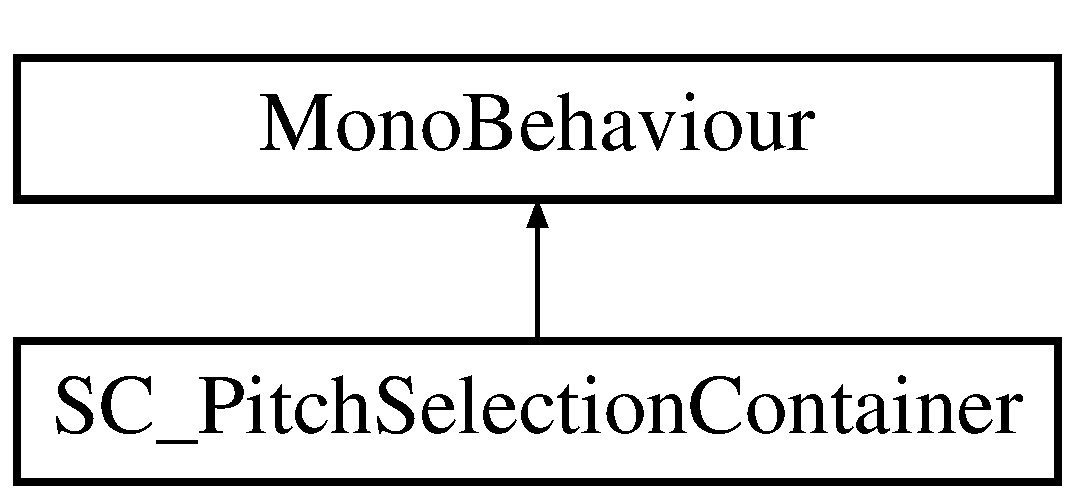
\includegraphics[height=2.000000cm]{class_s_c___pitch_selection_container}
\end{center}
\end{figure}
\subsection*{Public Member Functions}
\begin{DoxyCompactItemize}
\item 
\hyperlink{group___music_enums_ga508f69b199ea518f935486c990edac1d}{Music.\+P\+I\+T\+CH} \mbox{[}$\,$\mbox{]} \hyperlink{group___s_c___p_s_c_pub_func_ga05750cc6e1199f1522f8b87d6579dc34}{Get\+Selected\+Pitches} ()
\begin{DoxyCompactList}\small\item\em Gets the currently selected \hyperlink{group___music_enums_ga508f69b199ea518f935486c990edac1d}{pitches}/\hyperlink{group___music_enums_gade475b4382c7066d1af13e7c13c029b6}{drums}. \end{DoxyCompactList}\item 
void \hyperlink{group___s_c___p_s_c_pub_func_ga678ef561c5418e4bf43a5f9ed753f0f0}{Reset\+Pitches} ()
\begin{DoxyCompactList}\small\item\em Resets the selected selected \hyperlink{group___music_enums_ga508f69b199ea518f935486c990edac1d}{pitches}/\hyperlink{group___music_enums_gade475b4382c7066d1af13e7c13c029b6}{drums}. \end{DoxyCompactList}\item 
void \hyperlink{group___s_c___p_s_c_pub_func_ga0b85aab924084ebb49be4f64ad6f81e5}{Set\+Pitches} (\hyperlink{group___music_enums_ga508f69b199ea518f935486c990edac1d}{Music.\+P\+I\+T\+CH}\mbox{[}$\,$\mbox{]} a\+Pitches)
\begin{DoxyCompactList}\small\item\em Sets the selected \hyperlink{group___music_enums_ga508f69b199ea518f935486c990edac1d}{pitches}/\hyperlink{group___music_enums_gade475b4382c7066d1af13e7c13c029b6}{drums}. \end{DoxyCompactList}\item 
void \hyperlink{group___s_c___p_s_c_pub_func_ga08a0a4943359eb7f28c64aaf4cbc233c}{Set\+Up\+As\+Drum\+Selector} ()
\begin{DoxyCompactList}\small\item\em Sets up this selection container as a selector for \hyperlink{group___music_enums_gade475b4382c7066d1af13e7c13c029b6}{drums}. \end{DoxyCompactList}\item 
void \hyperlink{group___s_c___p_s_c_pub_func_gaf6e9338cfe7202df9787304e49afa24d}{Set\+Up\+As\+Pitch\+Selector} ()
\begin{DoxyCompactList}\small\item\em Sets up this selection container as a selector for \hyperlink{group___music_enums_ga508f69b199ea518f935486c990edac1d}{pitches}. \end{DoxyCompactList}\item 
void \hyperlink{group___s_c___p_s_c_handlers_gaa2afa8167100515d412cf751d9334f0c}{Handle\+Pitch\+Selection} (bool a\+Selected, int a\+Index)
\item 
void \hyperlink{group___s_c___p_s_c_handlers_ga8715b5976fdae2c56e05a60832553864}{On\+Rest\+Toggle} (bool a\+Is\+Rest\+Note)
\begin{DoxyCompactList}\small\item\em Handles switching between this \hyperlink{group___music_structs_struct_music_1_1_combined_note}{note} being a \hyperlink{group___doc_s_c___p_s_c_DocSC_PSCRest}{rest note} or not. \end{DoxyCompactList}\end{DoxyCompactItemize}
\subsection*{Private Attributes}
\begin{DoxyCompactItemize}
\item 
bool \hyperlink{group___s_c___p_s_c_priv_var_ga6eec175f775c35e2d0eb51dfe6def49f}{m\+Rest\+Note} = false
\begin{DoxyCompactList}\small\item\em Is this note currently set to be a rest note? \end{DoxyCompactList}\item 
List$<$ int $>$ \hyperlink{group___s_c___p_s_c_priv_var_ga5a8a5c31158f6af7f0c17d4fd03c5641}{m\+Selected\+Pitches} = null
\begin{DoxyCompactList}\small\item\em The selected \hyperlink{group___music_enums_ga508f69b199ea518f935486c990edac1d}{pitches} or \hyperlink{group___music_enums_gade475b4382c7066d1af13e7c13c029b6}{drums}. \end{DoxyCompactList}\item 
\hyperlink{class_s_c___pitch_selection_trigger}{S\+C\+\_\+\+Pitch\+Selection\+Trigger} \mbox{[}$\,$\mbox{]} \hyperlink{group___s_c___p_s_c_priv_var_ga8431846d376b98bc6de5a872cce2c596}{m\+Pitch\+Selection\+Triggers} = null
\begin{DoxyCompactList}\small\item\em The \hyperlink{group___doc_s_c___p_s_t}{triggers} that fire off an event when a \hyperlink{group___music_enums_ga508f69b199ea518f935486c990edac1d}{pitch} or \hyperlink{group___music_enums_gade475b4382c7066d1af13e7c13c029b6}{drum} is selected. \end{DoxyCompactList}\item 
Toggle \hyperlink{group___s_c___p_s_c_priv_var_gae4378d4e0b53501eb0f55b8af38a5a8c}{m\+Rest} = null
\begin{DoxyCompactList}\small\item\em The toggle switch for setting the \hyperlink{group___music_structs_struct_music_1_1_combined_note}{note} as a \hyperlink{group___doc_s_c___p_s_c_DocSC_PSCRest}{rest note}. \end{DoxyCompactList}\item 
Toggle \mbox{[}$\,$\mbox{]} \hyperlink{group___s_c___p_s_c_priv_var_ga25180add92621da773b024083d3a61af}{m\+Pitches} = null
\begin{DoxyCompactList}\small\item\em The toggle switches for each \hyperlink{group___music_enums_ga508f69b199ea518f935486c990edac1d}{pitch}/\hyperlink{group___music_enums_gade475b4382c7066d1af13e7c13c029b6}{drum}. \end{DoxyCompactList}\end{DoxyCompactItemize}


\subsection{Detailed Description}
C\# Class that contains the \hyperlink{group___doc_s_c___p_s_t}{pitch and drum selections} for a \hyperlink{group___music_structs_struct_music_1_1_combined_note}{note} in the \hyperlink{group___doc_s_c}{Song Creation Interface}. 

Though called a "Pitch Selection Container", this class is also used for selecting \hyperlink{group___music_enums_gade475b4382c7066d1af13e7c13c029b6}{drums}. The \hyperlink{group___music_enums_gade475b4382c7066d1af13e7c13c029b6}{drums} and \hyperlink{group___music_enums_ga508f69b199ea518f935486c990edac1d}{pitches} are typecast to integer in the \hyperlink{group___s_c___p_s_c_priv_var_ga5a8a5c31158f6af7f0c17d4fd03c5641}{list of selected pitches} anyway, so there is not much of a difference in how each are handled by this class. 

Definition at line 20 of file S\+C\+\_\+\+Pitch\+Selection\+Container.\+cs.



The documentation for this class was generated from the following file\+:\begin{DoxyCompactItemize}
\item 
D\+:/\+Documents/\+School Documents/2017\+Spring/\+E\+E\+C\+S542/\+V\+R\+Piano\+Project/\+Assets/\+Scripts/\+Audio/\+Song\+Creation/\hyperlink{_s_c___pitch_selection_container_8cs}{S\+C\+\_\+\+Pitch\+Selection\+Container.\+cs}\end{DoxyCompactItemize}

\hypertarget{class_s_c___pitch_selection_trigger}{}\section{S\+C\+\_\+\+Pitch\+Selection\+Trigger Class Reference}
\label{class_s_c___pitch_selection_trigger}\index{S\+C\+\_\+\+Pitch\+Selection\+Trigger@{S\+C\+\_\+\+Pitch\+Selection\+Trigger}}


Informs the \hyperlink{group___doc_s_c___p_s_c}{parent handler} about a \hyperlink{group___music_enums_ga508f69b199ea518f935486c990edac1d}{pitch} or \hyperlink{group___music_enums_gade475b4382c7066d1af13e7c13c029b6}{drum} being selected in the \hyperlink{group___doc_s_c}{Song Creation Interface}.  


Inheritance diagram for S\+C\+\_\+\+Pitch\+Selection\+Trigger\+:\begin{figure}[H]
\begin{center}
\leavevmode
\includegraphics[height=2.000000cm]{class_s_c___pitch_selection_trigger}
\end{center}
\end{figure}
\subsection*{Public Member Functions}
\begin{DoxyCompactItemize}
\item 
void \hyperlink{group___s_c___p_s_t_pub_func_ga0b334518dbdac5874adf9436cd2c7fed}{Set\+Handler} (\hyperlink{class_s_c___pitch_selection_container}{S\+C\+\_\+\+Pitch\+Selection\+Container} a\+Handler)
\begin{DoxyCompactList}\small\item\em Sets \hyperlink{group___doc_s_c___p_s_c}{the parent handler}. \end{DoxyCompactList}\item 
void \hyperlink{group___s_c___p_s_t_pub_func_ga0b4edbf9719a384aa5cf8d29d1065696}{Set\+Index} (int a\+Index)
\begin{DoxyCompactList}\small\item\em Sets the index of this trigger in \hyperlink{group___doc_s_c___p_s_c}{the parent handler}. \end{DoxyCompactList}\item 
void \hyperlink{group___s_c___p_s_t_pub_func_ga267db9aed38ba33ad44c26c84a1757df}{Set\+Selection} (bool a\+Selected)
\begin{DoxyCompactList}\small\item\em Sets whether or not this trigger is selected. \end{DoxyCompactList}\item 
void \hyperlink{group___s_c___p_s_t_handlers_ga5f4ea69eee3ed20cb09d56b7281ce861}{On\+Pitch\+Selected} (bool a\+Selected)
\begin{DoxyCompactList}\small\item\em Handles when a the trigger is selected via the \hyperlink{group___s_c___p_s_t_priv_var_ga1ecd33f50c82f6ffda81850438907a31}{associated toggle switch} by \hyperlink{group___s_c___p_s_c_handlers_gaa2afa8167100515d412cf751d9334f0c}{passing the event} to the \hyperlink{group___doc_s_c___p_s_c}{parent handler}. \end{DoxyCompactList}\end{DoxyCompactItemize}
\subsection*{Private Member Functions}
\begin{DoxyCompactItemize}
\item 
void \hyperlink{group___s_c___p_s_t_unity_gafa93dcca78e174eb2de6c4ea83b66a39}{Awake} ()
\begin{DoxyCompactList}\small\item\em Initializes the \hyperlink{class_s_c___pitch_selection_trigger}{S\+C\+\_\+\+Pitch\+Selection\+Trigger} by getting a reference to its \hyperlink{group___s_c___p_s_t_priv_var_ga1ecd33f50c82f6ffda81850438907a31}{toggle switch}. \end{DoxyCompactList}\end{DoxyCompactItemize}
\subsection*{Private Attributes}
\begin{DoxyCompactItemize}
\item 
int \hyperlink{group___s_c___p_s_t_priv_var_ga7d7771170c1f6cb1d6a9eb41e96a478f}{m\+Index} = -\/1
\begin{DoxyCompactList}\small\item\em The index of this trigger in \hyperlink{group___doc_s_c___p_s_c}{the parent handler}. \end{DoxyCompactList}\item 
\hyperlink{class_s_c___pitch_selection_container}{S\+C\+\_\+\+Pitch\+Selection\+Container} \hyperlink{group___s_c___p_s_t_priv_var_ga23cf7134e224e9718a99949979cd5078}{m\+Handler} = null
\begin{DoxyCompactList}\small\item\em \hyperlink{group___doc_s_c___p_s_c}{The parent handler}. \end{DoxyCompactList}\item 
Toggle \hyperlink{group___s_c___p_s_t_priv_var_ga1ecd33f50c82f6ffda81850438907a31}{m\+Toggle}
\begin{DoxyCompactList}\small\item\em The associated toggle switch that indicates whether or not the represented \hyperlink{group___music_enums_ga508f69b199ea518f935486c990edac1d}{pitch} or \hyperlink{group___music_enums_gade475b4382c7066d1af13e7c13c029b6}{drum} is selected. \end{DoxyCompactList}\end{DoxyCompactItemize}


\subsection{Detailed Description}
Informs the \hyperlink{group___doc_s_c___p_s_c}{parent handler} about a \hyperlink{group___music_enums_ga508f69b199ea518f935486c990edac1d}{pitch} or \hyperlink{group___music_enums_gade475b4382c7066d1af13e7c13c029b6}{drum} being selected in the \hyperlink{group___doc_s_c}{Song Creation Interface}. 

Definition at line 15 of file S\+C\+\_\+\+Pitch\+Selection\+Trigger.\+cs.



The documentation for this class was generated from the following file\+:\begin{DoxyCompactItemize}
\item 
D\+:/\+Documents/\+School Documents/2017\+Spring/\+E\+E\+C\+S542/\+V\+R\+Piano\+Project/\+Assets/\+Scripts/\+Audio/\+Song\+Creation/\hyperlink{_s_c___pitch_selection_trigger_8cs}{S\+C\+\_\+\+Pitch\+Selection\+Trigger.\+cs}\end{DoxyCompactItemize}

\hypertarget{class_song}{}\section{Song Class Reference}
\label{class_song}\index{Song@{Song}}


A C\# class that represents a song.  


\subsection*{Classes}
\begin{DoxyCompactItemize}
\item 
struct \hyperlink{group___song_structs_struct_song_1_1_combined_note_data}{Combined\+Note\+Data}
\begin{DoxyCompactList}\small\item\em A struct that contains data for both \hyperlink{group___music_structs_struct_music_1_1_percussion_note}{drums} and the \hyperlink{group___music_structs_struct_music_1_1_melody_note}{melody}.  \hyperlink{group___song_structs_struct_song_1_1_combined_note_data}{More...}\end{DoxyCompactList}\item 
struct \hyperlink{group___song_structs_struct_song_1_1_melody_note_data}{Melody\+Note\+Data}
\begin{DoxyCompactList}\small\item\em A struct for data related to \hyperlink{group___music_structs_struct_music_1_1_melody_note}{notes that contain pitches}.  \hyperlink{group___song_structs_struct_song_1_1_melody_note_data}{More...}\end{DoxyCompactList}\item 
struct \hyperlink{group___song_structs_struct_song_1_1_percussion_data}{Percussion\+Data}
\begin{DoxyCompactList}\small\item\em A struct for data related to \hyperlink{group___music_structs_struct_music_1_1_percussion_note}{drums}.  \hyperlink{group___song_structs_struct_song_1_1_percussion_data}{More...}\end{DoxyCompactList}\end{DoxyCompactItemize}
\subsection*{Public Types}
\begin{DoxyCompactItemize}
\item 
enum \hyperlink{group___song_enums_gae681a1f001333e39fc1cb4fea97bfe1b}{Song\+Type} \{ \hyperlink{group___song_enums_ggae681a1f001333e39fc1cb4fea97bfe1bace2c8aed9c2fa0cfbed56cbda4d8bf07}{Song\+Type.\+Empty}, 
\hyperlink{group___song_enums_ggae681a1f001333e39fc1cb4fea97bfe1bace2f3a5579d231b3b8f8b9e5fc46d361}{Song\+Type.\+Melody}, 
\hyperlink{group___song_enums_ggae681a1f001333e39fc1cb4fea97bfe1ba150deef06b13ddaeac61d0d2699ec61e}{Song\+Type.\+Drum\+Loop}, 
\hyperlink{group___song_enums_ggae681a1f001333e39fc1cb4fea97bfe1ba5130447d9fcb867ce341b3d17b117ced}{Song\+Type.\+Combined\+Melody\+And\+Percussion}
 \}\begin{DoxyCompactList}\small\item\em The possible types of songs. \end{DoxyCompactList}
\end{DoxyCompactItemize}
\subsection*{Public Member Functions}
\begin{DoxyCompactItemize}
\item 
\hyperlink{group___song_construct_gae2e6486a6a2f523b7c81de472d761ff5}{Song} ()
\begin{DoxyCompactList}\small\item\em The default constructor. \end{DoxyCompactList}\item 
\hyperlink{group___song_construct_ga157b9e8a0ca714707c2bf58bed5ebf4c}{Song} (string a\+Song\+File\+Path)
\begin{DoxyCompactList}\small\item\em A constructor that creates the song by \hyperlink{group___song_priv_func_ga5c8edd8f7ebeab0d93f5619a644c30f5}{loading a file}. \end{DoxyCompactList}\item 
void \hyperlink{group___song_pub_func_gab7c8fe4dc29f5ae7b7728c583fe51f7e}{Add\+Note} (\hyperlink{group___music_structs_struct_music_1_1_combined_note}{Music.\+Combined\+Note} a\+New\+Note)
\begin{DoxyCompactList}\small\item\em Adds a \hyperlink{group___music_structs_struct_music_1_1_combined_note}{note} to the \hyperlink{class_song}{Song}. \end{DoxyCompactList}\item 
int \hyperlink{group___song_pub_func_gaaaf3d27d474713d7d368e3fd4c570be0}{Get\+B\+PM} ()
\begin{DoxyCompactList}\small\item\em Gets the B\+PM of the song. \end{DoxyCompactList}\item 
\hyperlink{group___music_enums_ga508f69b199ea518f935486c990edac1d}{Music.\+P\+I\+T\+CH} \hyperlink{group___song_pub_func_gafaa104e8653edf64148260ecd400570f}{Get\+Highest\+Pitch} ()
\begin{DoxyCompactList}\small\item\em Gets the highest pitch in the song. \end{DoxyCompactList}\item 
\hyperlink{group___music_enums_ga508f69b199ea518f935486c990edac1d}{Music.\+P\+I\+T\+CH} \hyperlink{group___song_pub_func_gae4e71c8eb059cc9cf0b77e78971ab326}{Get\+Lowest\+Pitch} ()
\begin{DoxyCompactList}\small\item\em Gets the lowest pitch in the song. \end{DoxyCompactList}\item 
string \hyperlink{group___song_pub_func_ga705c433f2bfb5aede337698144b23c8b}{Get\+Name} ()
\begin{DoxyCompactList}\small\item\em Gets the name of the song. \end{DoxyCompactList}\item 
\hyperlink{group___music_structs_struct_music_1_1_combined_note}{Music.\+Combined\+Note} \hyperlink{group___song_pub_func_ga485c83c9278103fed23c532bba1252f0}{Get\+Note} (int a\+Index)
\begin{DoxyCompactList}\small\item\em Gets a \hyperlink{group___music_structs_struct_music_1_1_combined_note}{note} in the \hyperlink{class_song}{Song}. \end{DoxyCompactList}\item 
\hyperlink{group___song_structs_struct_song_1_1_combined_note_data}{Combined\+Note\+Data} \mbox{[}$\,$\mbox{]} \hyperlink{group___song_pub_func_gae3df1fd5448b7d9cefb0fed4af967985}{Get\+Note\+Data} ()
\begin{DoxyCompactList}\small\item\em Converts the \hyperlink{group___music_structs_struct_music_1_1_combined_note}{notes} in the song to Note\+Data. \end{DoxyCompactList}\item 
List$<$ \hyperlink{group___music_structs_struct_music_1_1_combined_note}{Music.\+Combined\+Note} $>$ \hyperlink{group___song_pub_func_ga842675b7691fca074ee394031afc7675}{Get\+All\+Notes} ()
\begin{DoxyCompactList}\small\item\em Returns a list of the \hyperlink{group___music_structs_struct_music_1_1_combined_note}{notes} in the \hyperlink{class_song}{Song}. \end{DoxyCompactList}\item 
int \hyperlink{group___song_pub_func_gad124d0af146885327f8ac455bc013b63}{Get\+Num\+Notes} ()
\begin{DoxyCompactList}\small\item\em Gets the number of \hyperlink{group___music_structs_struct_music_1_1_combined_note}{notes} in the \hyperlink{class_song}{Song}. \end{DoxyCompactList}\item 
\hyperlink{group___song_enums_gae681a1f001333e39fc1cb4fea97bfe1b}{Song\+Type} \hyperlink{group___song_pub_func_gabae5b5d8f727b2d9da7867a99347f86b}{Get\+Song\+Type} ()
\begin{DoxyCompactList}\small\item\em Gets the \hyperlink{group___song_enums_gae681a1f001333e39fc1cb4fea97bfe1b}{type of song} that the \hyperlink{class_song}{Song} is. \end{DoxyCompactList}\item 
\hyperlink{group___music_structs_struct_music_1_1_time_signature}{Music.\+Time\+Signature} \hyperlink{group___song_pub_func_ga26315bb6d554d46e2eba2ac03ee70cc1}{Get\+Time\+Signature} ()
\begin{DoxyCompactList}\small\item\em Gets the \hyperlink{group___music_structs_struct_music_1_1_time_signature}{time signature} of the \hyperlink{class_song}{Song}. \end{DoxyCompactList}\item 
void \hyperlink{group___song_pub_func_ga856634e047b8c35160958c3aa53d6b28}{Remove\+Note} (int a\+Index)
\begin{DoxyCompactList}\small\item\em Removes a note from the song. \end{DoxyCompactList}\item 
void \hyperlink{group___song_pub_func_ga326d61c75339080057a02c6decb0cde3}{Replace\+Note} (\hyperlink{group___music_structs_struct_music_1_1_combined_note}{Music.\+Combined\+Note} a\+Note, int a\+Index)
\begin{DoxyCompactList}\small\item\em Replaces a note at a given index. \end{DoxyCompactList}\item 
void \hyperlink{group___song_pub_func_gaa65bbba1af7192edff7e0f848029013b}{Set\+B\+PM} (int a\+B\+PM)
\begin{DoxyCompactList}\small\item\em Sets the default \hyperlink{group___audio_DefBPM}{B\+PM} of the \hyperlink{class_song}{Song}. \end{DoxyCompactList}\item 
void \hyperlink{group___song_pub_func_ga1efefe19fd0c5962f7f8ed16c65cd835}{Set\+B\+PM} (float a\+B\+PM)
\begin{DoxyCompactList}\small\item\em Sets the default \hyperlink{group___audio_DefBPM}{B\+PM} of the \hyperlink{class_song}{Song}. \end{DoxyCompactList}\item 
void \hyperlink{group___song_pub_func_gacb01510cf72657fc7c64bb6ba00c2c56}{Set\+Name} (string a\+Song\+Name)
\begin{DoxyCompactList}\small\item\em Sets the \hyperlink{group___song_priv_var_ga6a5e6c1e4aa92939e2b5c1e3d9908df8}{name} of the \hyperlink{class_song}{Song}. \end{DoxyCompactList}\item 
void \hyperlink{group___song_pub_func_gaf9f2c7e6f4400f6f9854e68e70a49470}{Set\+Time\+Signature} (\hyperlink{group___music_structs_struct_music_1_1_time_signature}{Music.\+Time\+Signature} a\+Time\+Signature)
\begin{DoxyCompactList}\small\item\em Sets the \hyperlink{group___music_structs_struct_music_1_1_time_signature}{time signature} of the \hyperlink{class_song}{Song}. \end{DoxyCompactList}\item 
void \hyperlink{group___song_pub_func_ga70b0f6021c3b0590c561a88e3d1e5c2f}{Write\+Song\+To\+File} ()
\begin{DoxyCompactList}\small\item\em Writes the song to a file. The file will be stored in Streaming\+Assets/\+Songs/. \end{DoxyCompactList}\end{DoxyCompactItemize}
\subsection*{Static Public Member Functions}
\begin{DoxyCompactItemize}
\item 
static int \hyperlink{group___song_stat_func_ga03712f6defbff25d5a1cd964e4bc3211}{Get\+Note\+Length\+In\+Samples} (int a\+B\+PM, int a\+Sample\+Rate, \hyperlink{group___music_enums_gaf11b5f079adbb21c800b9eca1c5c3cbd}{Music.\+N\+O\+T\+E\+\_\+\+L\+E\+N\+G\+TH} a\+Note\+Length, \hyperlink{group___music_structs_struct_music_1_1_time_signature}{Music.\+Time\+Signature} a\+Time\+Signature)
\begin{DoxyCompactList}\small\item\em Gets the number of waveform samples required to accurately represent the \hyperlink{group___music_enums_gaf11b5f079adbb21c800b9eca1c5c3cbd}{length of a note} for a given \hyperlink{group___audio_DefBPM}{B\+PM} and \hyperlink{group___music_structs_struct_music_1_1_time_signature}{time signature}. \end{DoxyCompactList}\end{DoxyCompactItemize}
\subsection*{Static Public Attributes}
\begin{DoxyCompactItemize}
\item 
static string \hyperlink{group___song_const_ga95247572cf734f9e8b35973de4eeb1a4}{S\+O\+N\+G\+\_\+\+F\+I\+L\+E\+\_\+\+P\+A\+TH} = Application.\+streaming\+Assets\+Path + \char`\"{}/Songs/\char`\"{}
\begin{DoxyCompactList}\small\item\em The path of the folder that contains \hyperlink{class_song}{Song} files. \end{DoxyCompactList}\end{DoxyCompactItemize}
\subsection*{Private Member Functions}
\begin{DoxyCompactItemize}
\item 
void \hyperlink{group___song_priv_func_ga5c8edd8f7ebeab0d93f5619a644c30f5}{Load\+Song\+From\+File} (string a\+Song\+File\+Path)
\begin{DoxyCompactList}\small\item\em Loads a \hyperlink{group___song_group_DocSongFileFormat}{Song file} and uses it to set the values for this \hyperlink{class_song}{Song}. \end{DoxyCompactList}\item 
\hyperlink{group___music_enums_gade475b4382c7066d1af13e7c13c029b6}{Music.\+D\+R\+UM} \mbox{[}$\,$\mbox{]} \hyperlink{group___song_priv_func_gaaa4ca12f0885a34cbfb09bb7a1db178b}{Parse\+Drums} (string a\+String\+From\+File)
\begin{DoxyCompactList}\small\item\em Parses the \hyperlink{group___music_enums_gade475b4382c7066d1af13e7c13c029b6}{drums} from a string in a \hyperlink{group___song_group_DocSongFileFormat}{Song file}. \end{DoxyCompactList}\item 
\hyperlink{group___music_enums_ga508f69b199ea518f935486c990edac1d}{Music.\+P\+I\+T\+CH} \mbox{[}$\,$\mbox{]} \hyperlink{group___song_priv_func_gacf6fee93921e1a5edbc477c0898c357a}{Parse\+Pitches} (string a\+String\+From\+File)
\begin{DoxyCompactList}\small\item\em Parses the \hyperlink{group___music_enums_ga508f69b199ea518f935486c990edac1d}{pitches} from a string in a \hyperlink{group___song_group_DocSongFileFormat}{Song file}. \end{DoxyCompactList}\item 
void \hyperlink{group___song_priv_func_ga5f837e6b7f576732fa38747caa057621}{Search\+For\+Highest\+Pitch} ()
\begin{DoxyCompactList}\small\item\em Searches through the notes for the highest pitch. \end{DoxyCompactList}\item 
void \hyperlink{group___song_priv_func_gac2e812c6385529eb7a9be5082c7bde75}{Search\+For\+Lowest\+Pitch} ()
\begin{DoxyCompactList}\small\item\em Searches through the notes for the lowest pitch. \end{DoxyCompactList}\item 
void \hyperlink{group___song_priv_func_ga9a1d6eba1576c3631d3c0331196d9ae2}{Update\+Song\+Type} ()
\begin{DoxyCompactList}\small\item\em Updates the \hyperlink{group___song_enums_gae681a1f001333e39fc1cb4fea97bfe1b}{type of song} that the \hyperlink{class_song}{Song} is. \end{DoxyCompactList}\end{DoxyCompactItemize}
\subsection*{Private Attributes}
\begin{DoxyCompactItemize}
\item 
int \hyperlink{group___song_priv_var_ga3341fbbd9c0c58fe6514623e6b6c5a1e}{m\+B\+PM} = 120
\begin{DoxyCompactList}\small\item\em The default \hyperlink{group___audio_DefBPM}{B\+PM} of the \hyperlink{class_song}{Song}. \end{DoxyCompactList}\item 
int \hyperlink{group___song_priv_var_ga3dbce17d96b434d4492280c39cff1778}{m\+Num\+Drum\+Notes}
\begin{DoxyCompactList}\small\item\em The number of \hyperlink{group___music_structs_struct_music_1_1_combined_note}{notes} that have \hyperlink{group___music_structs_struct_music_1_1_percussion_note}{drums}. \end{DoxyCompactList}\item 
int \hyperlink{group___song_priv_var_gaf55b4fd2df0457ba1306a75ac3fdc8b1}{m\+Num\+Musical\+Notes}
\begin{DoxyCompactList}\small\item\em The number of \hyperlink{group___music_structs_struct_music_1_1_combined_note}{notes} that have \hyperlink{group___music_structs_struct_music_1_1_melody_note}{pitches}. \end{DoxyCompactList}\item 
List$<$ \hyperlink{group___music_structs_struct_music_1_1_combined_note}{Music.\+Combined\+Note} $>$ \hyperlink{group___song_priv_var_ga674bc904a1f856d485d5fb7fe84bac85}{m\+Notes} = null
\begin{DoxyCompactList}\small\item\em The \hyperlink{group___music_structs_struct_music_1_1_combined_note}{notes} of the \hyperlink{class_song}{Song}. \end{DoxyCompactList}\item 
\hyperlink{group___music_enums_ga508f69b199ea518f935486c990edac1d}{Music.\+P\+I\+T\+CH} \hyperlink{group___song_priv_var_ga2dcd39d9add609e9df56a94057441dcc}{m\+Highest\+Pitch} = \hyperlink{group___music_enums_gga508f69b199ea518f935486c990edac1da9c5959e6f08f10d0edbadf5be1f33c53}{Music.\+P\+I\+T\+C\+H.\+C0}
\begin{DoxyCompactList}\small\item\em The highest \hyperlink{group___music_enums_ga508f69b199ea518f935486c990edac1d}{pitch} in the \hyperlink{class_song}{Song}. \end{DoxyCompactList}\item 
\hyperlink{group___music_enums_ga508f69b199ea518f935486c990edac1d}{Music.\+P\+I\+T\+CH} \hyperlink{group___song_priv_var_ga293976ef4c2050687a81edfbf77b4fc1}{m\+Lowest\+Pitch} = \hyperlink{group___music_enums_gga508f69b199ea518f935486c990edac1da18fc90be5b8124af983421d29bfc4352}{Music.\+P\+I\+T\+C\+H.\+B9}
\begin{DoxyCompactList}\small\item\em The lowest \hyperlink{group___music_enums_ga508f69b199ea518f935486c990edac1d}{pitch} in the \hyperlink{class_song}{Song}. \end{DoxyCompactList}\item 
\hyperlink{group___music_structs_struct_music_1_1_time_signature}{Music.\+Time\+Signature} \hyperlink{group___song_priv_var_ga2b2dcc0e83e49f7303b6a1371877b25e}{m\+Time\+Signature}
\begin{DoxyCompactList}\small\item\em The \hyperlink{group___music_structs_struct_music_1_1_time_signature}{time signature} of the \hyperlink{class_song}{Song}. \end{DoxyCompactList}\item 
\hyperlink{group___song_enums_gae681a1f001333e39fc1cb4fea97bfe1b}{Song\+Type} \hyperlink{group___song_priv_var_gaf3b9d0f461522324f897b746311b43c5}{m\+Type} = \hyperlink{group___song_enums_ggae681a1f001333e39fc1cb4fea97bfe1bace2c8aed9c2fa0cfbed56cbda4d8bf07}{Song\+Type.\+Empty}
\begin{DoxyCompactList}\small\item\em The \hyperlink{group___song_enums_gae681a1f001333e39fc1cb4fea97bfe1b}{type of song} that this \hyperlink{class_song}{Song} is. \end{DoxyCompactList}\item 
string \hyperlink{group___song_priv_var_ga6a5e6c1e4aa92939e2b5c1e3d9908df8}{m\+Name} = null
\begin{DoxyCompactList}\small\item\em The name of the \hyperlink{class_song}{Song}. \end{DoxyCompactList}\end{DoxyCompactItemize}


\subsection{Detailed Description}
A C\# class that represents a song. 

This class\textquotesingle{}s responsibilities include\+: \begin{DoxyItemize}
\item Serving as a container for a pre-\/arranged series of \hyperlink{group___music_structs_struct_music_1_1_combined_note}{notes}. \item Converting the \hyperlink{group___music_structs_struct_music_1_1_combined_note}{abstract representions of musical notes} into \hyperlink{group___song_structs_struct_song_1_1_combined_note_data}{a form that relates to the actual waveforms of the audio}. \item Saving and loading copies of itself to/from a file. \end{DoxyItemize}


Definition at line 18 of file Song.\+cs.



The documentation for this class was generated from the following file\+:\begin{DoxyCompactItemize}
\item 
D\+:/\+Documents/\+School Documents/2017\+Spring/\+E\+E\+C\+S542/\+V\+R\+Piano\+Project/\+Assets/\+Scripts/\+Audio/\+Song\+Management/\hyperlink{_song_8cs}{Song.\+cs}\end{DoxyCompactItemize}

\hypertarget{class_song_creation_manager}{}\section{Song\+Creation\+Manager Class Reference}
\label{class_song_creation_manager}\index{Song\+Creation\+Manager@{Song\+Creation\+Manager}}


A script that manages all of the \hyperlink{group___doc_s_c}{Song Creation Interface}.  


Inheritance diagram for Song\+Creation\+Manager\+:\begin{figure}[H]
\begin{center}
\leavevmode
\includegraphics[height=2.000000cm]{class_song_creation_manager}
\end{center}
\end{figure}
\subsection*{Classes}
\begin{DoxyCompactItemize}
\item 
class \hyperlink{group___s_c_m_nest_class_class_song_creation_manager_1_1_song_creation_selection_container}{Song\+Creation\+Selection\+Container}
\end{DoxyCompactItemize}
\subsection*{Public Member Functions}
\begin{DoxyCompactItemize}
\item 
void \hyperlink{group___s_c_m_handlers_gae5930497314c77bd9c52c083b2f3e82e}{On\+B\+P\+M\+Change} (float a\+B\+PM)
\begin{DoxyCompactList}\small\item\em Handles a change in the song\textquotesingle{}s default B\+PM. \end{DoxyCompactList}\item 
void \hyperlink{group___s_c_m_handlers_gaed512eb78e060a40616e6e31ce029440}{On\+Create\+Note} ()
\begin{DoxyCompactList}\small\item\em Creates a new note in the song. \end{DoxyCompactList}\item 
void \hyperlink{group___s_c_m_handlers_gacb552a4f02b22d7c10a8420eb1431201}{On\+Edit\+Event} (\hyperlink{class_s_c___note_display_panel}{S\+C\+\_\+\+Note\+Display\+Panel} a\+Panel)
\begin{DoxyCompactList}\small\item\em Handles when a note panel is selected for editing. \end{DoxyCompactList}\item 
void \hyperlink{group___s_c_m_handlers_gaf12d6326ad2175a51f688504372be784}{On\+Modify\+Note} ()
\begin{DoxyCompactList}\small\item\em Modifies a \hyperlink{group___music_structs_struct_music_1_1_combined_note}{note} in the \hyperlink{class_song}{Song}. \end{DoxyCompactList}\item 
void \hyperlink{group___s_c_m_handlers_gafb394a0b00c8f9c0959d901faf9131c7}{On\+Play\+Song} ()
\begin{DoxyCompactList}\small\item\em Plays the \hyperlink{class_song}{Song} being created. \end{DoxyCompactList}\item 
void \hyperlink{group___s_c_m_handlers_ga1f1e9a15a6c339282fb94085d4862605}{On\+Remove\+Note} (int a\+Index)
\begin{DoxyCompactList}\small\item\em Removes a \hyperlink{group___music_structs_struct_music_1_1_combined_note}{note} from the \hyperlink{class_song}{Song} being created. \end{DoxyCompactList}\item 
void \hyperlink{group___s_c_m_handlers_gafd5e9f72e7a15cb77994c59fbbf8b769}{On\+Save\+Song} ()
\begin{DoxyCompactList}\small\item\em Saves the \hyperlink{class_song}{Song} to a file. \end{DoxyCompactList}\item 
void \hyperlink{group___s_c_m_handlers_ga45e79bb31be34e3e2cc47bd6a6563b40}{On\+Velocity\+Change} (float a\+Velocity)
\begin{DoxyCompactList}\small\item\em Handles a change in the \hyperlink{group___audio_DefVel}{velocity} for a \hyperlink{group___music_structs_struct_music_1_1_combined_note}{note} in the \hyperlink{class_song}{Song} being created. \end{DoxyCompactList}\item 
void \hyperlink{group___s_c_m_handlers_gac39b0d849c680dda1e047c3e7d848b51}{Unload\+Song\+Creation\+Interface} ()
\begin{DoxyCompactList}\small\item\em Goes back to the Audio\+Testing\+Interface scene. \end{DoxyCompactList}\end{DoxyCompactItemize}
\subsection*{Private Member Functions}
\begin{DoxyCompactItemize}
\item 
void \hyperlink{group___s_c_m_unity_ga2747d8e56d35acf19b90525b861cc7dd}{Awake} ()
\begin{DoxyCompactList}\small\item\em Initializes the \hyperlink{group___doc_s_c}{Song Creation Interface} by getting references to all of the modules within the scene. \end{DoxyCompactList}\item 
void \hyperlink{group___s_c_m_handlers_ga1747d021ddb36a8c2c172315d6fbb3a8}{On\+Load\+Song\+Button\+Clicked} ()
\begin{DoxyCompactList}\small\item\em Handles the \hyperlink{group___s_c_m_priv_var_ga7851ecd194d87e14fa186fc76e154222}{Load Song button} being clicked by loading the \hyperlink{group___doc_s_c___l_s_d}{Load Song Dialog}. \end{DoxyCompactList}\item 
void \hyperlink{group___s_c_m_handlers_gae3791e700c2e12f1dd705c4b951ec260}{On\+Load\+Song} (\hyperlink{class_song}{Song} a\+Song)
\begin{DoxyCompactList}\small\item\em Loads a \hyperlink{class_song}{Song} into the \hyperlink{group___doc_s_c}{Song Creation Interface}. \end{DoxyCompactList}\end{DoxyCompactItemize}
\subsection*{Private Attributes}
\begin{DoxyCompactItemize}
\item 
string \hyperlink{group___s_c_m_const_ga821945ef78c5b9411d7861b42407591e}{L\+O\+A\+D\+\_\+\+S\+O\+N\+G\+\_\+\+D\+I\+A\+L\+O\+G\+\_\+\+P\+A\+TH} = \char`\"{}Audio/Prefabs/Song\+Creation/Load\+Song\+Dialog\+Prefab\char`\"{}
\begin{DoxyCompactList}\small\item\em The path to load the \hyperlink{group___doc_s_c___l_s_d}{Load Song Dialog}\textquotesingle{}s prefab. \end{DoxyCompactList}\item 
bool \hyperlink{group___s_c_m_priv_var_gad2a61787c63fb8770d3c8100adfae9cf}{m\+Editing} = false
\begin{DoxyCompactList}\small\item\em Whether or not a note is being modified. \end{DoxyCompactList}\item 
Button \hyperlink{group___s_c_m_priv_var_gae702ec5de2c75149b8c650db9ac260a6}{m\+A\+T\+I\+Button} = null
\begin{DoxyCompactList}\small\item\em The button to reload the audio testing interface. \end{DoxyCompactList}\item 
Button \hyperlink{group___s_c_m_priv_var_ga7851ecd194d87e14fa186fc76e154222}{m\+Load\+Song\+Button} = null
\begin{DoxyCompactList}\small\item\em The button to load a song. \end{DoxyCompactList}\item 
Button \hyperlink{group___s_c_m_priv_var_gac17f83788e480bb97160d17bbe69aab3}{m\+New\+Note\+Button} = null
\begin{DoxyCompactList}\small\item\em The button to add a new note with the chosen values. \end{DoxyCompactList}\item 
Button \hyperlink{group___s_c_m_priv_var_ga4ba18826907a0efbeb2ad62444124657}{m\+Play\+Song\+Button} = null
\begin{DoxyCompactList}\small\item\em The button to play the song. \end{DoxyCompactList}\item 
Button \hyperlink{group___s_c_m_priv_var_ga7f15c9af246da41fe9f7aafb16744214}{m\+Reset\+Pitches\+Button} = null
\begin{DoxyCompactList}\small\item\em The button to reset the pitch selections. \end{DoxyCompactList}\item 
Button \hyperlink{group___s_c_m_priv_var_gaf43eabc869ead30d8ac7027e07502289}{m\+Save\+Song\+Button} = null
\begin{DoxyCompactList}\small\item\em The button to save the song to a file. \end{DoxyCompactList}\item 
Input\+Field \hyperlink{group___s_c_m_priv_var_ga0dd175c73748d5cc8ba4621f36126255}{m\+Song\+Name\+Input\+Field} = null
\begin{DoxyCompactList}\small\item\em The input field to name the song. \end{DoxyCompactList}\item 
\hyperlink{group___music_enums_gaf11b5f079adbb21c800b9eca1c5c3cbd}{Music.\+N\+O\+T\+E\+\_\+\+L\+E\+N\+G\+TH} \hyperlink{group___s_c_m_priv_var_gaa137adb1c99e9ee59adcfbf7d0cf6249}{m\+Last\+Length} = \hyperlink{group___music_enums_ggaf11b5f079adbb21c800b9eca1c5c3cbdab50339a10e1de285ac99d4c3990b8693}{Music.\+N\+O\+T\+E\+\_\+\+L\+E\+N\+G\+T\+H.\+N\+O\+NE}
\begin{DoxyCompactList}\small\item\em The length used to create the last note. Used for special handling of drum loops. \end{DoxyCompactList}\item 
\hyperlink{class_s_c___note_display_container}{S\+C\+\_\+\+Note\+Display\+Container} \hyperlink{group___s_c_m_priv_var_ga308f19d1b2020fc625c12dd08ee16b1c}{m\+Note\+Display} = null
\begin{DoxyCompactList}\small\item\em The container to show the notes for the song. \end{DoxyCompactList}\item 
\hyperlink{class_s_c___note_display_panel}{S\+C\+\_\+\+Note\+Display\+Panel} \hyperlink{group___s_c_m_priv_var_gad063b650cf7112be19edaf1a2033ea4d}{m\+Edit\+Panel} = null
\begin{DoxyCompactList}\small\item\em The panel that was selected to be edited. \end{DoxyCompactList}\item 
\hyperlink{class_s_c___pitch_selection_container}{S\+C\+\_\+\+Pitch\+Selection\+Container} \hyperlink{group___s_c_m_priv_var_gac8be873b8259a0ddf76b4fa6d7d2d072}{m\+Drum\+Selector} = null
\begin{DoxyCompactList}\small\item\em The container for choosing drums. \end{DoxyCompactList}\item 
\hyperlink{class_s_c___pitch_selection_container}{S\+C\+\_\+\+Pitch\+Selection\+Container} \hyperlink{group___s_c_m_priv_var_gab84821120cace4099edfb42c52d2af63}{m\+Pitch\+Selector} = null
\begin{DoxyCompactList}\small\item\em The container for choosing pitches. \end{DoxyCompactList}\item 
Slider \hyperlink{group___s_c_m_priv_var_ga87ac3691ad7848394e51442f29d9659d}{m\+B\+P\+M\+Slider} = null
\begin{DoxyCompactList}\small\item\em The slider for the B\+PM of the song. \end{DoxyCompactList}\item 
Slider \hyperlink{group___s_c_m_priv_var_ga7316e5e8f15d1574fc6cb4bd739bbf0a}{m\+Velocity\+Slider} = null
\begin{DoxyCompactList}\small\item\em The slider for the velocity of the new note. \end{DoxyCompactList}\item 
\hyperlink{class_song}{Song} \hyperlink{group___s_c_m_priv_var_gabd8329149faef65a689650d951a9abc9}{m\+Song} = null
\begin{DoxyCompactList}\small\item\em The song being created. \end{DoxyCompactList}\item 
\hyperlink{group___s_c_m_nest_class_class_song_creation_manager_1_1_song_creation_selection_container}{Song\+Creation\+Selection\+Container} \hyperlink{group___s_c_m_priv_var_gadb8dedf80fbe474a1c94cdc95d088a6f}{m\+Length\+Panel} = null
\begin{DoxyCompactList}\small\item\em The panel to choose a length for the new note. \end{DoxyCompactList}\item 
\hyperlink{group___s_c_m_nest_class_class_song_creation_manager_1_1_song_creation_selection_container}{Song\+Creation\+Selection\+Container} \hyperlink{group___s_c_m_priv_var_ga86a44007a4b127d7aa61f75dd34a3409}{m\+Offset\+Panel} = null
\begin{DoxyCompactList}\small\item\em The panel to choose an offset for the new note. \end{DoxyCompactList}\item 
\hyperlink{class_virtual_instrument_manager}{Virtual\+Instrument\+Manager} \hyperlink{group___s_c_m_priv_var_ga7822ac42d20a4577db66808f000decfb}{m\+V\+IM} = null
\begin{DoxyCompactList}\small\item\em The virtual instrument manager. \end{DoxyCompactList}\end{DoxyCompactItemize}


\subsection{Detailed Description}
A script that manages all of the \hyperlink{group___doc_s_c}{Song Creation Interface}. 

This class is the central hub for all of the \hyperlink{group___doc_s_c}{Song Creation Interface}. It connects each modules within the interface to each other and uses them to create a \hyperlink{class_song}{Song}. 

Definition at line 19 of file Song\+Creation\+Manager.\+cs.



The documentation for this class was generated from the following file\+:\begin{DoxyCompactItemize}
\item 
D\+:/\+Documents/\+School Documents/2017\+Spring/\+E\+E\+C\+S542/\+V\+R\+Piano\+Project/\+Assets/\+Scripts/\+Audio/\+Song\+Creation/\hyperlink{_song_creation_manager_8cs}{Song\+Creation\+Manager.\+cs}\end{DoxyCompactItemize}

\hypertarget{class_song_manager_class}{}\section{Song\+Manager\+Class Class Reference}
\label{class_song_manager_class}\index{Song\+Manager\+Class@{Song\+Manager\+Class}}


C\# class that handles loading and playing Songs.  


\subsection*{Public Member Functions}
\begin{DoxyCompactItemize}
\item 
\hyperlink{group___s_m_construct_gacd94623c6402ad7c7af2f725265d0e4d}{Song\+Manager\+Class} ()
\begin{DoxyCompactList}\small\item\em Initializes the \hyperlink{class_song_manager_class}{Song\+Manager\+Class} by creating its lists of songs. \end{DoxyCompactList}\item 
void \hyperlink{group___s_m_pub_func_ga1a228cb2a64e55448ccf9d1d618f05b7}{Add\+Song} (\hyperlink{class_song}{Song} a\+Song)
\begin{DoxyCompactList}\small\item\em Adds a \hyperlink{class_song}{Song} to the Song\+Manager. \end{DoxyCompactList}\item 
List$<$ string $>$ \hyperlink{group___s_m_pub_func_ga87bd14c75666b13bd02510c5b7080784}{Get\+Combined\+Song\+Names} ()
\begin{DoxyCompactList}\small\item\em Gets the names of the loaded \hyperlink{group___song_group_DocSongCombined}{songs that have both percussion and melody}. \end{DoxyCompactList}\item 
List$<$ \hyperlink{class_song}{Song} $>$ \hyperlink{group___s_m_pub_func_ga413595693011bd6021dfd6eb941bf0e6}{Get\+Combined\+Songs} ()
\begin{DoxyCompactList}\small\item\em Gets the loaded \hyperlink{group___song_group_DocSongCombined}{songs that have both percussion and melody}. \end{DoxyCompactList}\item 
List$<$ string $>$ \hyperlink{group___s_m_pub_func_ga90e0aeb3117c5db6c667a23252bf45f6}{Get\+Drum\+Loop\+Names} ()
\begin{DoxyCompactList}\small\item\em Gets the names of the loaded \hyperlink{group___song_group_DocSongDrumLoop}{drum loops}. \end{DoxyCompactList}\item 
List$<$ \hyperlink{class_song}{Song} $>$ \hyperlink{group___s_m_pub_func_ga354a675f296f9a733ad6d76fea7429dd}{Get\+Drum\+Loops} ()
\begin{DoxyCompactList}\small\item\em Gets the loaded \hyperlink{group___song_group_DocSongDrumLoop}{drum loops}. \end{DoxyCompactList}\item 
List$<$ string $>$ \hyperlink{group___s_m_pub_func_ga59df8468ac771fc8eb1a5f2025e6c5a8}{Get\+Melody\+Names} ()
\begin{DoxyCompactList}\small\item\em Gets the names of the loaded \hyperlink{group___song_group_DocSongMelody}{melodies}. \end{DoxyCompactList}\item 
List$<$ \hyperlink{class_song}{Song} $>$ \hyperlink{group___s_m_pub_func_ga7d46ab1949725dd7c3c00ac3975916fe}{Get\+Melodies} ()
\begin{DoxyCompactList}\small\item\em Gets the loaded \hyperlink{group___song_group_DocSongMelody}{melodies}. \end{DoxyCompactList}\item 
int \hyperlink{group___s_m_pub_func_gac41e94dbaa3f2db83a6d86466526f76c}{Get\+Number\+Of\+Combined\+Songs} ()
\begin{DoxyCompactList}\small\item\em Gets the number of loaded Songs that \hyperlink{group___song_group_DocSongCombined}{have both drums and melody}. \end{DoxyCompactList}\item 
int \hyperlink{group___s_m_pub_func_ga97d32492e08ca62787088888e78589b7}{Get\+Number\+Of\+Drum\+Loops} ()
\begin{DoxyCompactList}\small\item\em Gets the number of loaded \hyperlink{group___song_group_DocSongDrumLoop}{drum loops}. \end{DoxyCompactList}\item 
int \hyperlink{group___s_m_pub_func_gae1d2222909f1d9a1f761591c7154f42c}{Get\+Number\+Of\+Melodies} ()
\begin{DoxyCompactList}\small\item\em Gets the number of loaded \hyperlink{group___song_group_DocSongMelody}{melodies}. \end{DoxyCompactList}\item 
\hyperlink{class_song}{Song} \hyperlink{group___s_m_pub_func_gafe818c55bd858c52c95a2fa7a566006a}{Get\+Song\+By\+Name} (string a\+Song\+Name)
\begin{DoxyCompactList}\small\item\em Gets a specific \hyperlink{class_song}{Song}. \end{DoxyCompactList}\item 
List$<$ string $>$ \hyperlink{group___s_m_pub_func_ga2a9455a763e35cfb6b242a82f7d797ae}{Get\+Song\+Names} ()
\begin{DoxyCompactList}\small\item\em Gets the names of the loaded Songs. \end{DoxyCompactList}\item 
List$<$ \hyperlink{class_song}{Song} $>$ \hyperlink{group___s_m_pub_func_ga3bf6a6d42a7c5e94cc85ba10eb9e6edb}{Get\+Songs} ()
\begin{DoxyCompactList}\small\item\em Gets all of the Songs. \end{DoxyCompactList}\end{DoxyCompactItemize}
\subsection*{Private Member Functions}
\begin{DoxyCompactItemize}
\item 
void \hyperlink{group___s_m_priv_func_ga73d6d3b38a160fd73b63b786b9cd384a}{Load\+Songs} ()
\begin{DoxyCompactList}\small\item\em Loads Songs in the folder \char`\"{}\+A\+P\+P\+\_\+\+P\+A\+T\+H/\+Streaming\+Assets/\+Audio/\+Songs/\char`\"{}. \end{DoxyCompactList}\end{DoxyCompactItemize}
\subsection*{Private Attributes}
\begin{DoxyCompactItemize}
\item 
Dictionary$<$ string, \hyperlink{class_song}{Song} $>$ \hyperlink{group___s_m_priv_var_gaf6b4ff41b8da95d10ad3db62df111faa}{m\+Combined\+Songs} = null
\begin{DoxyCompactList}\small\item\em The loaded songs that \hyperlink{group___song_group_DocSongCombined}{have both percussion and melody}. \end{DoxyCompactList}\item 
Dictionary$<$ string, \hyperlink{class_song}{Song} $>$ \hyperlink{group___s_m_priv_var_ga84f25335035755448d11acb9287360f2}{m\+Drum\+Loops} = null
\begin{DoxyCompactList}\small\item\em The loaded \hyperlink{group___song_group_DocSongDrumLoop}{drum loops}. \end{DoxyCompactList}\item 
Dictionary$<$ string, \hyperlink{class_song}{Song} $>$ \hyperlink{group___s_m_priv_var_ga935e80f645d0546003f7df8443b79242}{m\+Melodies} = null
\begin{DoxyCompactList}\small\item\em The loaded \hyperlink{group___song_group_DocSongMelody}{melodies}. \end{DoxyCompactList}\item 
int \hyperlink{group___s_m_priv_var_gae423c7b9efd0e2ef721820318200e5f9}{m\+Num\+Combined\+Songs} = 0
\begin{DoxyCompactList}\small\item\em The number of loaded songs that \hyperlink{group___song_group_DocSongCombined}{have both percussion and melody}. \end{DoxyCompactList}\item 
int \hyperlink{group___s_m_priv_var_ga0ea9b6c8343a9b2cbe0eb375edaef247}{m\+Num\+Drum\+Loops} = 0
\begin{DoxyCompactList}\small\item\em The number of loaded \hyperlink{group___song_group_DocSongDrumLoop}{drum loops}. \end{DoxyCompactList}\item 
int \hyperlink{group___s_m_priv_var_ga58ea3b4f794b9e444eece384ae6e8197}{m\+Num\+Melodies} = 0
\begin{DoxyCompactList}\small\item\em The number of loaded \hyperlink{group___song_group_DocSongMelody}{melodies}. \end{DoxyCompactList}\end{DoxyCompactItemize}


\subsection{Detailed Description}
C\# class that handles loading and playing Songs. 

\begin{DoxyNote}{Note}
Meant to only be used as a child of the \hyperlink{group___v_i_m}{Virtual Instrument Manager}.
\end{DoxyNote}
\begin{DoxySeeAlso}{See also}
\hyperlink{group___v_i_m_pub_ga33dae94932c10c66db76a0eebec76b01}{Virtual\+Instrument\+Manager\+::\+Song\+Manager} 
\end{DoxySeeAlso}


Definition at line 15 of file Song\+Manager\+Class.\+cs.



The documentation for this class was generated from the following file\+:\begin{DoxyCompactItemize}
\item 
D\+:/\+Documents/\+School Documents/2017\+Spring/\+E\+E\+C\+S542/\+V\+R\+Piano\+Project/\+Assets/\+Scripts/\+Audio/\+Song\+Management/\hyperlink{_song_manager_class_8cs}{Song\+Manager\+Class.\+cs}\end{DoxyCompactItemize}

\hypertarget{class_virtual_instrument}{}\section{Virtual\+Instrument Class Reference}
\label{class_virtual_instrument}\index{Virtual\+Instrument@{Virtual\+Instrument}}


A base class that contains generic functions and values relating to \hyperlink{group___v_i}{Virtual Instruments}.  


Inheritance diagram for Virtual\+Instrument\+:\begin{figure}[H]
\begin{center}
\leavevmode
\includegraphics[height=2.000000cm]{class_virtual_instrument}
\end{center}
\end{figure}
\subsection*{Public Member Functions}
\begin{DoxyCompactItemize}
\item 
\hyperlink{group___v_i_base_construct_ga7b438b5f812fa0d3a6e91d74a3c261c9}{Virtual\+Instrument} (\hyperlink{class_virtual_instrument_manager}{Virtual\+Instrument\+Manager} a\+Parent)
\begin{DoxyCompactList}\small\item\em Generic constructor. Sets default values and values that are common to all \hyperlink{group___v_i}{Virtual Instruments}. \end{DoxyCompactList}\item 
int \hyperlink{group___v_i_base_pub_func_gacddf07c08c3a8154a6934be22f539788}{Get\+Built\+In\+Dynamics\+Threshold\+Index} (int a\+Velocity)
\begin{DoxyCompactList}\small\item\em Gets the index for which sound file to use for a \hyperlink{group___music_enums_ga508f69b199ea518f935486c990edac1d}{pitch} at a given \hyperlink{group___audio_DefVel}{velocity}. \end{DoxyCompactList}\item 
int \mbox{[}$\,$\mbox{]} \hyperlink{group___v_i_base_pub_func_gac8fc20c49c1b97b6787ed1b3e0073a7f}{Get\+Built\+In\+Dynamics\+Thresholds} ()
\begin{DoxyCompactList}\small\item\em Gets the ranges for which sound file to use for a \hyperlink{group___audio_DefVel}{velocity}. \end{DoxyCompactList}\item 
float \hyperlink{group___v_i_base_pub_func_gae638c68bd0e79d0b99495be69e50f49d}{Get\+Adjusted\+Velocity\+Factor} (int a\+Velocity)
\begin{DoxyCompactList}\small\item\em Gets the factor by which a note\textquotesingle{}s waveform is scaled in order to account for \hyperlink{group___audio_DefVel}{velocity}. \end{DoxyCompactList}\item 
\hyperlink{group___music_enums_ga508f69b199ea518f935486c990edac1d}{Music.\+P\+I\+T\+CH} \hyperlink{group___v_i_base_pub_func_ga859f3e73b1d28051cecf0ecd1c8b10ee}{Get\+Highest\+Supported\+Pitch} ()
\begin{DoxyCompactList}\small\item\em Gets the highest \hyperlink{group___music_enums_ga508f69b199ea518f935486c990edac1d}{pitch} that this instrument can play. \end{DoxyCompactList}\item 
\hyperlink{group___music_enums_ga508f69b199ea518f935486c990edac1d}{Music.\+P\+I\+T\+CH} \hyperlink{group___v_i_base_pub_func_gac42b3915bbfec60b83650abd701d0690}{Get\+Lowest\+Supported\+Pitch} ()
\begin{DoxyCompactList}\small\item\em Gets the lowest \hyperlink{group___music_enums_ga508f69b199ea518f935486c990edac1d}{pitch} that this instrument can play. \end{DoxyCompactList}\item 
int \hyperlink{group___v_i_base_pub_func_ga6ce5a7b3406269ea433be721d7d11177}{Get\+Num\+Of\+Supported\+Pitches} ()
\begin{DoxyCompactList}\small\item\em Gets the total number of \hyperlink{group___music_enums_ga508f69b199ea518f935486c990edac1d}{pitches} that this instrument can play. \end{DoxyCompactList}\item 
float \mbox{[}$\,$\mbox{]}\mbox{[}$\,$\mbox{]} \hyperlink{group___v_i_base_pub_func_gaf715f7c3bbd2f1a2fa543b2f0684f8a6}{Get\+Audio\+Data\+For\+Pitch} (\hyperlink{group___music_enums_ga508f69b199ea518f935486c990edac1d}{Music.\+P\+I\+T\+CH} a\+Pitch)
\begin{DoxyCompactList}\small\item\em Gets the raw audio data of each built-\/in dynamics value for a given \hyperlink{group___music_enums_ga508f69b199ea518f935486c990edac1d}{pitch}. \end{DoxyCompactList}\item 
float \hyperlink{group___v_i_base_pub_func_gabea22c3ab14c6989b9357da0bf052fbc}{Get\+Sample\+Interval} ()
\begin{DoxyCompactList}\small\item\em Gets the time interval between waveform samples for this instrument. \end{DoxyCompactList}\item 
int \hyperlink{group___v_i_base_pub_func_ga8be9d452abaf025dc7270c36b3cf379a}{Get\+Sample\+Rate} ()
\begin{DoxyCompactList}\small\item\em Gets the sample rate for the wav files used to create the instrument. \end{DoxyCompactList}\item 
bool \hyperlink{group___v_i_base_pub_func_gae8b5ac2e3402dfc50ea43f0e91fd9a29}{Is\+Loaded} ()
\begin{DoxyCompactList}\small\item\em Gets whether or not the instrument has loaded. \end{DoxyCompactList}\item 
bool \hyperlink{group___v_i_base_pub_func_ga89655451c108a7ad5cb96ab308e33937}{Is\+Pitch\+Supported} (\hyperlink{group___music_enums_ga508f69b199ea518f935486c990edac1d}{Music.\+P\+I\+T\+CH} a\+Pitch)
\begin{DoxyCompactList}\small\item\em Gets whether or not the instrument can play a specific \hyperlink{group___music_enums_ga508f69b199ea518f935486c990edac1d}{pitch}. \end{DoxyCompactList}\end{DoxyCompactItemize}
\subsection*{Static Public Attributes}
\begin{DoxyCompactItemize}
\item 
static float \hyperlink{group___v_i_base_const_ga69a037919b64e1e3e0f2b949b2b6af2c}{S\+A\+M\+P\+L\+E\+\_\+\+I\+N\+T\+E\+R\+V\+AL} = 1.\+1337e-\/5f
\begin{DoxyCompactList}\small\item\em The number of seconds between waveform samples. \end{DoxyCompactList}\end{DoxyCompactItemize}
\subsection*{Protected Member Functions}
\begin{DoxyCompactItemize}
\item 
void \hyperlink{group___v_i_base_pro_func_gadbd95083895b09465fbc5b18115a1dbc}{Load\+Audio\+Clip\+For\+Pitch} (\hyperlink{group___music_enums_ga508f69b199ea518f935486c990edac1d}{Music.\+P\+I\+T\+CH} a\+Pitch)
\begin{DoxyCompactList}\small\item\em Loads all the audio clips associated with a pitch. \end{DoxyCompactList}\item 
void \hyperlink{group___v_i_base_pro_func_ga873242f52d077ca4305b0b69a0100b55}{Load\+Audio\+Clips} ()
\begin{DoxyCompactList}\small\item\em Loads the audio clips for the instrument. \hyperlink{group___v_i_base_virt_func_gaacfc9521214176292bfb9665556fb991}{Virtual\+Instrument\+::\+Create\+Filenames} must be called prior to this function in order to actually find the files. \end{DoxyCompactList}\item 
virtual void \hyperlink{group___v_i_base_virt_func_gaacfc9521214176292bfb9665556fb991}{Create\+Filenames} ()
\begin{DoxyCompactList}\small\item\em Creates the filenames for the sample files. \end{DoxyCompactList}\item 
virtual void \hyperlink{group___v_i_base_virt_func_ga995456c03ee54543b285188c51c29a07}{Initialize\+Built\+In\+Dynamics} ()
\begin{DoxyCompactList}\small\item\em Initializes variables related to \hyperlink{group___audio_DefBID}{Built-\/\+In Dynamics}. \end{DoxyCompactList}\end{DoxyCompactItemize}
\subsection*{Protected Attributes}
\begin{DoxyCompactItemize}
\item 
bool \hyperlink{group___v_i_base_pro_var_ga47dbd8aa02ab32b8f802adfd2d3d81de}{m\+Is\+Drum}
\begin{DoxyCompactList}\small\item\em Whether or not the virtual instrument is a \hyperlink{class_drum_kit}{drum kit}. \end{DoxyCompactList}\item 
bool \hyperlink{group___v_i_base_pro_var_ga8978807d1878db5aae91fbd057c46097}{m\+Loaded}
\begin{DoxyCompactList}\small\item\em Whether or not the virtual instrument is loaded. \end{DoxyCompactList}\item 
float \hyperlink{group___v_i_base_pro_var_ga20c1d3d25ea666378d72c833d160ae2e}{m\+Sample\+Interval}
\begin{DoxyCompactList}\small\item\em The waveform sample interval of the virtual instrument. \end{DoxyCompactList}\item 
float \mbox{[}$\,$\mbox{]}\mbox{[}$\,$\mbox{]}\mbox{[}$\,$\mbox{]} \hyperlink{group___v_i_base_pro_var_ga52e76d9b74408660584676035a92a2c6}{m\+Audio\+Data}
\begin{DoxyCompactList}\small\item\em The waveform samples of the virtual instrument. The indices are mapped according to \mbox{[}\hyperlink{group___audio_DefBID}{Built\+In\+Dynamics\+Index}\mbox{]}\mbox{[}\hyperlink{group___music_enums_ga508f69b199ea518f935486c990edac1d}{Pitch}\mbox{]}\mbox{[}Waveform\+Sample\mbox{]}. \end{DoxyCompactList}\item 
int \hyperlink{group___v_i_base_pro_var_ga9a602db8c9833ce75d95dd453c27d341}{m\+Num\+Files}
\begin{DoxyCompactList}\small\item\em The number of sample files. \end{DoxyCompactList}\item 
int \hyperlink{group___v_i_base_pro_var_gac265f64f759d267ee1e1680f8d387011}{m\+Num\+Built\+In\+Dynamics}
\begin{DoxyCompactList}\small\item\em The number of \hyperlink{group___audio_DefBID}{Built-\/in Dynamics}. \end{DoxyCompactList}\item 
int \hyperlink{group___v_i_base_pro_var_gafc759a16324cf9b3f230bcbf040afcd2}{m\+Num\+Supported\+Pitches}
\begin{DoxyCompactList}\small\item\em The number of \hyperlink{group___music_enums_ga508f69b199ea518f935486c990edac1d}{pitches} supported by the instrument. \end{DoxyCompactList}\item 
int \hyperlink{group___v_i_base_pro_var_ga80b3d2ff29b27698eea6bcf2f8ddc5d7}{m\+Sample\+Rate}
\begin{DoxyCompactList}\small\item\em The sample rate of the virtual instrument. \end{DoxyCompactList}\item 
int \mbox{[}$\,$\mbox{]} \hyperlink{group___v_i_base_pro_var_gae3db4264dc2a96e99ea680c6d637e6bf}{m\+Built\+In\+Dynamics\+Thresholds}
\begin{DoxyCompactList}\small\item\em The \hyperlink{group___audio_DefBIDThresh}{thresholds} for when to use a specific sound file. \end{DoxyCompactList}\item 
\hyperlink{group___music_enums_ga508f69b199ea518f935486c990edac1d}{Music.\+P\+I\+T\+CH} \hyperlink{group___v_i_base_pro_var_ga3cae52b1bcc0178a8a6b03c7aaf7aac8}{m\+Lowest\+Supported\+Pitch}
\begin{DoxyCompactList}\small\item\em The lowest supported \hyperlink{group___music_enums_ga508f69b199ea518f935486c990edac1d}{pitch} of the instrument. \end{DoxyCompactList}\item 
\hyperlink{group___music_enums_ga508f69b199ea518f935486c990edac1d}{Music.\+P\+I\+T\+CH} \hyperlink{group___v_i_base_pro_var_ga61fb2c33b53a0f663047779d7ceb18f3}{m\+Highest\+Supported\+Pitch}
\begin{DoxyCompactList}\small\item\em The highest supported \hyperlink{group___music_enums_ga508f69b199ea518f935486c990edac1d}{pitch} of the instrument. \end{DoxyCompactList}\item 
string \hyperlink{group___v_i_base_pro_var_gac428224be859933d720a9c533fdb5643}{m\+Filepath}
\begin{DoxyCompactList}\small\item\em The base filepath for the samples. \end{DoxyCompactList}\item 
string \mbox{[}$\,$\mbox{]} \hyperlink{group___v_i_base_pro_var_gab2add474ca506357688b5dd08cac4cb5}{m\+Filenames}
\begin{DoxyCompactList}\small\item\em An array of filenames for the samples. \end{DoxyCompactList}\item 
string \mbox{[}$\,$\mbox{]} \hyperlink{group___v_i_base_pro_var_ga87961e72f25fbc2256b614a394aa6f13}{m\+Built\+In\+Dynamics}
\begin{DoxyCompactList}\small\item\em The names of the \hyperlink{group___audio_DefBID}{Built-\/\+In Dynamics}. \end{DoxyCompactList}\item 
\hyperlink{class_virtual_instrument_manager}{Virtual\+Instrument\+Manager} \hyperlink{group___v_i_base_pro_var_gae4a87a656d9448cfea28215a6b9c3840}{m\+Parent}
\begin{DoxyCompactList}\small\item\em The \hyperlink{group___v_i_m}{manager} for this instrument. \end{DoxyCompactList}\end{DoxyCompactItemize}
\subsection*{Private Member Functions}
\begin{DoxyCompactItemize}
\item 
void \hyperlink{group___v_i_base_priv_func_gaecd4f9ead08a03be878b2085055a975c}{Normalize\+Audio\+Clips\+For\+Pitch} (\hyperlink{group___music_enums_ga508f69b199ea518f935486c990edac1d}{Music.\+P\+I\+T\+CH} a\+Pitch, Audio\+Clip\mbox{[}$\,$\mbox{]} a\+Clips)
\begin{DoxyCompactList}\small\item\em Normalizes the data from the audio clips and puts them in the m\+Audio\+Data member variable. \end{DoxyCompactList}\item 
void \hyperlink{group___v_i_base_priv_func_ga0262de8cfb1e671b01ba76de2e9d140a}{Normalize\+Audio\+Clips} (Audio\+Clip\mbox{[}$\,$\mbox{]}\mbox{[}$\,$\mbox{]} a\+Audio\+Clips)
\begin{DoxyCompactList}\small\item\em Normalizes the data from the audio clips and puts them in the m\+Audio\+Data member variable. \end{DoxyCompactList}\end{DoxyCompactItemize}
\subsection*{Private Attributes}
\begin{DoxyCompactItemize}
\item 
const float \hyperlink{group___v_i_base_const_gaf060c000443f92784bd8db8d866d8b2a}{N\+O\+R\+M\+A\+L\+I\+Z\+E\+D\+\_\+\+P\+E\+AK} = -\/.\+1f
\begin{DoxyCompactList}\small\item\em The peak of the waveform after it\textquotesingle{}s normalized. \end{DoxyCompactList}\end{DoxyCompactItemize}


\subsection{Detailed Description}
A base class that contains generic functions and values relating to \hyperlink{group___v_i}{Virtual Instruments}. 

The base \hyperlink{class_virtual_instrument}{Virtual\+Instrument} class performs tasks such as retrieving raw audio data from wav files and note mapping. This is a C\# class rather than a Unity-\/specific class, so it is not attached to any Game\+Object itself. This is because it should only interact with the \hyperlink{group___v_i_m}{Virtual Instrument Manager}, and other classes should go through the \hyperlink{group___v_i_m}{manager} to get information about the instrument. This hiding of information is done for ease of using the audio code with other parts of the program by making all interactions with the audio go through a common hub.

~\newline
 This class is meant to be the base class for implementing specific instruments. It is not meant to be used by itself as anything other than a container that is checked at runtime. Also, every \hyperlink{group___v_i}{Virtual Instrument} is meant to be used as-\/is, so there is no modification that can be done on this class by other classes that do not inherit it. 

Definition at line 26 of file Virtual\+Instrument.\+cs.



The documentation for this class was generated from the following file\+:\begin{DoxyCompactItemize}
\item 
D\+:/\+Documents/\+School Documents/2017\+Spring/\+E\+E\+C\+S542/\+V\+R\+Piano\+Project/\+Assets/\+Scripts/\+Audio/\+Virtual\+Instrument/\hyperlink{_virtual_instrument_8cs}{Virtual\+Instrument.\+cs}\end{DoxyCompactItemize}

\hypertarget{class_virtual_instrument_manager}{}\section{Virtual\+Instrument\+Manager Class Reference}
\label{class_virtual_instrument_manager}\index{Virtual\+Instrument\+Manager@{Virtual\+Instrument\+Manager}}


The central hub for all audio management.  


Inheritance diagram for Virtual\+Instrument\+Manager\+:\begin{figure}[H]
\begin{center}
\leavevmode
\includegraphics[height=2.000000cm]{class_virtual_instrument_manager}
\end{center}
\end{figure}
\subsection*{Classes}
\begin{DoxyCompactItemize}
\item 
class \hyperlink{group___v_i_m_event_types_class_virtual_instrument_manager_1_1_audio_finished_event}{Audio\+Finished\+Event}
\begin{DoxyCompactList}\small\item\em Notifies when the audio is finished. There\textquotesingle{}s no handler for this, but it can be used by other classes who need to be notified.  \hyperlink{group___v_i_m_event_types_class_virtual_instrument_manager_1_1_audio_finished_event}{More...}\end{DoxyCompactList}\item 
class \hyperlink{group___v_i_m_event_types_class_virtual_instrument_manager_1_1_change_instrument_event}{Change\+Instrument\+Event}
\begin{DoxyCompactList}\small\item\em A type of event that is invoked whenever a new instrument should be loaded.  \hyperlink{group___v_i_m_event_types_class_virtual_instrument_manager_1_1_change_instrument_event}{More...}\end{DoxyCompactList}\item 
class \hyperlink{group___v_i_m_event_types_class_virtual_instrument_manager_1_1_change_note_range_event}{Change\+Note\+Range\+Event}
\begin{DoxyCompactList}\small\item\em A type of event that is invoked whenever the range of playable pitches should change.  \hyperlink{group___v_i_m_event_types_class_virtual_instrument_manager_1_1_change_note_range_event}{More...}\end{DoxyCompactList}\item 
class \hyperlink{group___v_i_m_event_types_class_virtual_instrument_manager_1_1_drum_kit_loaded_event}{Drum\+Kit\+Loaded\+Event}
\begin{DoxyCompactList}\small\item\em A type of event that is invoked in order to signal that the drum kit has loaded.  \hyperlink{group___v_i_m_event_types_class_virtual_instrument_manager_1_1_drum_kit_loaded_event}{More...}\end{DoxyCompactList}\item 
struct \hyperlink{group__filter_params_struct_virtual_instrument_manager_1_1_echo_filter_parameters}{Echo\+Filter\+Parameters}
\begin{DoxyCompactList}\small\item\em A struct that holds the parameters for the echo filter.  \hyperlink{group__filter_params_struct_virtual_instrument_manager_1_1_echo_filter_parameters}{More...}\end{DoxyCompactList}\item 
class \hyperlink{group___v_i_m_event_types_class_virtual_instrument_manager_1_1_instrument_loaded_event}{Instrument\+Loaded\+Event}
\begin{DoxyCompactList}\small\item\em A type of event that is invoked in order to signal that the instrument has loaded.  \hyperlink{group___v_i_m_event_types_class_virtual_instrument_manager_1_1_instrument_loaded_event}{More...}\end{DoxyCompactList}\item 
class \hyperlink{group___v_i_m_event_types_class_virtual_instrument_manager_1_1_modify_echo_filter_event}{Modify\+Echo\+Filter\+Event}
\begin{DoxyCompactList}\small\item\em A type of event that is invoked in order to modify the echo filter.  \hyperlink{group___v_i_m_event_types_class_virtual_instrument_manager_1_1_modify_echo_filter_event}{More...}\end{DoxyCompactList}\item 
class \hyperlink{group___v_i_m_event_types_class_virtual_instrument_manager_1_1_modify_reverb_filter_event}{Modify\+Reverb\+Filter\+Event}
\begin{DoxyCompactList}\small\item\em A type of event that is invoked in order to modify the reverb filter.  \hyperlink{group___v_i_m_event_types_class_virtual_instrument_manager_1_1_modify_reverb_filter_event}{More...}\end{DoxyCompactList}\item 
class \hyperlink{group___v_i_m_event_types_class_virtual_instrument_manager_1_1_pause_drum_loop_event}{Pause\+Drum\+Loop\+Event}
\begin{DoxyCompactList}\small\item\em A type of event that is invoked in order to pause a drum loop.  \hyperlink{group___v_i_m_event_types_class_virtual_instrument_manager_1_1_pause_drum_loop_event}{More...}\end{DoxyCompactList}\item 
class \hyperlink{group___v_i_m_event_types_class_virtual_instrument_manager_1_1_pause_song_event}{Pause\+Song\+Event}
\begin{DoxyCompactList}\small\item\em A type of event that is invoked in order to pause a song.  \hyperlink{group___v_i_m_event_types_class_virtual_instrument_manager_1_1_pause_song_event}{More...}\end{DoxyCompactList}\item 
class \hyperlink{group___v_i_m_event_types_class_virtual_instrument_manager_1_1_play_drum_loop_event}{Play\+Drum\+Loop\+Event}
\begin{DoxyCompactList}\small\item\em A type of event that is invoked in order to play a drum loop.  \hyperlink{group___v_i_m_event_types_class_virtual_instrument_manager_1_1_play_drum_loop_event}{More...}\end{DoxyCompactList}\item 
class \hyperlink{group___v_i_m_event_types_class_virtual_instrument_manager_1_1_play_note_event}{Play\+Note\+Event}
\begin{DoxyCompactList}\small\item\em A type of event that is invoked whenever a note should be played.  \hyperlink{group___v_i_m_event_types_class_virtual_instrument_manager_1_1_play_note_event}{More...}\end{DoxyCompactList}\item 
class \hyperlink{group___v_i_m_event_types_class_virtual_instrument_manager_1_1_play_song_event}{Play\+Song\+Event}
\begin{DoxyCompactList}\small\item\em A type of event that is invoked in order to play a song.  \hyperlink{group___v_i_m_event_types_class_virtual_instrument_manager_1_1_play_song_event}{More...}\end{DoxyCompactList}\item 
class \hyperlink{group___v_i_m_event_types_class_virtual_instrument_manager_1_1_release_note_event}{Release\+Note\+Event}
\begin{DoxyCompactList}\small\item\em A type of event that is invoked whenever a note should fade out as though the key was released.  \hyperlink{group___v_i_m_event_types_class_virtual_instrument_manager_1_1_release_note_event}{More...}\end{DoxyCompactList}\item 
class \hyperlink{group___v_i_m_event_types_class_virtual_instrument_manager_1_1_resume_drum_loop_event}{Resume\+Drum\+Loop\+Event}
\begin{DoxyCompactList}\small\item\em Resumes a drum loop.  \hyperlink{group___v_i_m_event_types_class_virtual_instrument_manager_1_1_resume_drum_loop_event}{More...}\end{DoxyCompactList}\item 
class \hyperlink{group___v_i_m_event_types_class_virtual_instrument_manager_1_1_resume_song_event}{Resume\+Song\+Event}
\begin{DoxyCompactList}\small\item\em Resumes a song.  \hyperlink{group___v_i_m_event_types_class_virtual_instrument_manager_1_1_resume_song_event}{More...}\end{DoxyCompactList}\item 
struct \hyperlink{group__filter_params_struct_virtual_instrument_manager_1_1_reverb_filter_parameters}{Reverb\+Filter\+Parameters}
\begin{DoxyCompactList}\small\item\em A struct that holds the parameters for the reverb filter.  \hyperlink{group__filter_params_struct_virtual_instrument_manager_1_1_reverb_filter_parameters}{More...}\end{DoxyCompactList}\item 
class \hyperlink{group___v_i_m_event_types_class_virtual_instrument_manager_1_1_stop_drum_loop_event}{Stop\+Drum\+Loop\+Event}
\begin{DoxyCompactList}\small\item\em Stops a drum loop.  \hyperlink{group___v_i_m_event_types_class_virtual_instrument_manager_1_1_stop_drum_loop_event}{More...}\end{DoxyCompactList}\item 
class \hyperlink{group___v_i_m_event_types_class_virtual_instrument_manager_1_1_stop_song_event}{Stop\+Song\+Event}
\begin{DoxyCompactList}\small\item\em Stops a song.  \hyperlink{group___v_i_m_event_types_class_virtual_instrument_manager_1_1_stop_song_event}{More...}\end{DoxyCompactList}\end{DoxyCompactItemize}
\subsection*{Public Member Functions}
\begin{DoxyCompactItemize}
\item 
void \hyperlink{group___v_i_m_unity_gab92bac4e22476ffe39fc40f49fbd6ae5}{Awake} ()
\begin{DoxyCompactList}\small\item\em Called when the object is created. Sets the default values, sets up the events, and begins loading the instrument. \end{DoxyCompactList}\item 
\hyperlink{group___music_enums_ga508f69b199ea518f935486c990edac1d}{Music.\+P\+I\+T\+CH} \mbox{[}$\,$\mbox{]} \hyperlink{group___v_i_m_pub_func_ga119e0c582106fc9ecc2631e39d71d681}{Get\+Active\+Notes} ()
\begin{DoxyCompactList}\small\item\em Gets the array of active notes. \end{DoxyCompactList}\item 
\hyperlink{group___audio_testing_class_a_t_i___diagnostics}{A\+T\+I\+\_\+\+Diagnostics} \hyperlink{group___v_i_m_pub_func_ga7e60bc3c5464d8f34f0d56def675bcc6}{Get\+Diagnostics\+Handler} ()
\begin{DoxyCompactList}\small\item\em Gets the \hyperlink{group___audio_testing_class_a_t_i___diagnostics}{audio diagnostics handler}. \end{DoxyCompactList}\item 
\hyperlink{group___music_enums_ga508f69b199ea518f935486c990edac1d}{Music.\+P\+I\+T\+CH} \hyperlink{group___v_i_m_pub_func_gab58eabfbcdaa60a3a7dbd972df6f57a6}{Get\+Highest\+Active\+Note} ()
\begin{DoxyCompactList}\small\item\em Gets the highest active note. \end{DoxyCompactList}\item 
\hyperlink{group___music_enums_ga508f69b199ea518f935486c990edac1d}{Music.\+P\+I\+T\+CH} \hyperlink{group___v_i_m_pub_func_ga586d5ed5b0fe832d66c9a99aa160ceee}{Get\+Highest\+Supported\+Note} ()
\begin{DoxyCompactList}\small\item\em Gets the highest note that is supported by the loaded instrument. \end{DoxyCompactList}\item 
\hyperlink{class_virtual_instrument}{Virtual\+Instrument} \hyperlink{group___v_i_m_pub_func_gac39a3e411417dc010f0e4fd8f146fbc3}{Get\+Instrument} ()
\begin{DoxyCompactList}\small\item\em Gets the loaded \hyperlink{class_virtual_instrument}{Virtual\+Instrument}. \end{DoxyCompactList}\item 
\hyperlink{group___music_enums_ga508f69b199ea518f935486c990edac1d}{Music.\+P\+I\+T\+CH} \hyperlink{group___v_i_m_pub_func_ga09bfbd0756fc8110c877e5b59c104bcd}{Get\+Lowest\+Active\+Note} ()
\begin{DoxyCompactList}\small\item\em Gets the lowest active note. \end{DoxyCompactList}\item 
\hyperlink{group___music_enums_ga508f69b199ea518f935486c990edac1d}{Music.\+P\+I\+T\+CH} \hyperlink{group___v_i_m_pub_func_gaeb152486450d6c6dc50078e1644c4c6a}{Get\+Lowest\+Supported\+Note} ()
\begin{DoxyCompactList}\small\item\em Gets the lowest note that is supported by the loaded instrument. \end{DoxyCompactList}\item 
\hyperlink{class_musical_typing_handler}{Musical\+Typing\+Handler} \hyperlink{group___v_i_m_pub_func_gae6701458a23a3f14db90501f871d4d0d}{Get\+Musical\+Typing\+Handler} ()
\item 
int \hyperlink{group___v_i_m_pub_func_ga3d6c823b1c1083eac8202f6c89e60b48}{Get\+Num\+Active\+Notes} ()
\begin{DoxyCompactList}\small\item\em Gets the number of notes that currently can be played. \end{DoxyCompactList}\item 
void \hyperlink{group___v_i_m_handlers_ga8e79286073756c31e08fecd59ce04fa7}{On\+Change\+Instrument\+Event} (\hyperlink{group___music_enums_gabfce60192305965558a36e368ebd67c3}{Music.\+I\+N\+S\+T\+R\+U\+M\+E\+N\+T\+\_\+\+T\+Y\+PE} a\+New\+Instrument\+Type)
\begin{DoxyCompactList}\small\item\em Called whenever an instrument should be loaded. \end{DoxyCompactList}\item 
void \hyperlink{group___v_i_m_handlers_ga660c766dceebfc830de2cf96686692df}{On\+Change\+Note\+Range\+Event} (\hyperlink{group___music_enums_ga508f69b199ea518f935486c990edac1d}{Music.\+P\+I\+T\+CH} a\+New\+Lowest\+Pitch)
\begin{DoxyCompactList}\small\item\em Called whenever the range of active notes should be changed. \end{DoxyCompactList}\item 
void \hyperlink{group___v_i_m_handlers_gac7d5b65484e450a400e32ab416ebc9f6}{On\+Instrument\+Loaded} ()
\begin{DoxyCompactList}\small\item\em Called whenever the instrument has finished loading. It begins loading the Note\+Output\+Objects. \end{DoxyCompactList}\item 
void \hyperlink{group___v_i_m_handlers_gae504c6ded8eb68ffb117c207fc25d99d}{On\+Modify\+Echo\+Filter\+Event} (\hyperlink{group__filter_params_struct_virtual_instrument_manager_1_1_echo_filter_parameters}{Echo\+Filter\+Parameters} a\+Parameters)
\begin{DoxyCompactList}\small\item\em Called whenever the echo filter should be modified. \end{DoxyCompactList}\item 
void \hyperlink{group___v_i_m_handlers_ga2b310217971075b1b2db67d68fbbea5a}{On\+Modify\+Reverb\+Filter\+Event} (\hyperlink{group__filter_params_struct_virtual_instrument_manager_1_1_reverb_filter_parameters}{Reverb\+Filter\+Parameters} a\+Parameters)
\begin{DoxyCompactList}\small\item\em Called whenever the reverb filter should be modified. \end{DoxyCompactList}\item 
void \hyperlink{group___v_i_m_handlers_ga30cd7f00fea55becd6d90f0ec737510a}{On\+Pause\+Drum\+Loop\+Event} ()
\begin{DoxyCompactList}\small\item\em Handles pausing a drum loop. \end{DoxyCompactList}\item 
void \hyperlink{group___v_i_m_handlers_gad052b3cc53b35b25631f9b399be489ae}{On\+Pause\+Song\+Event} ()
\begin{DoxyCompactList}\small\item\em Handles pausing a song. \end{DoxyCompactList}\item 
void \hyperlink{group___v_i_m_handlers_gae2e2010b9a36ae2409466181ae0b9679}{On\+Play\+Drum\+Loop\+Event} (\hyperlink{class_song}{Song} a\+Loop)
\begin{DoxyCompactList}\small\item\em Begins playing a drum loop. It creates an array of audio data from each note of the \hyperlink{class_song}{Song} and sends it to the right \hyperlink{class_note_output_object}{Note\+Output\+Object}. \end{DoxyCompactList}\item 
void \hyperlink{group___v_i_m_handlers_ga80b3821df3b1488a150f6062638f105c}{On\+Play\+Note\+Event} (\hyperlink{group___music_enums_ga508f69b199ea518f935486c990edac1d}{Music.\+P\+I\+T\+CH} a\+Note\+To\+Play, int a\+Velocity)
\begin{DoxyCompactList}\small\item\em Called whenever a note should be played. Uses the appropriate \hyperlink{class_note_output_object}{Note\+Output\+Object} to play the note. \end{DoxyCompactList}\item 
void \hyperlink{group___v_i_m_handlers_ga7fd877a7d429403abbfd2728aa63c056}{On\+Play\+Song\+Event} (\hyperlink{class_song}{Song} a\+Song)
\begin{DoxyCompactList}\small\item\em Begins playing a song. It creates an array of audio data from each note of the \hyperlink{class_song}{Song} and sends it to the right \hyperlink{class_note_output_object}{Note\+Output\+Object}. \end{DoxyCompactList}\item 
void \hyperlink{group___v_i_m_handlers_ga0f0a34c251d154131f9ea130a54dc989}{On\+Release\+Note\+Event} (\hyperlink{group___music_enums_ga508f69b199ea518f935486c990edac1d}{Music.\+P\+I\+T\+CH} a\+Note\+To\+Release)
\begin{DoxyCompactList}\small\item\em Called whenever a note should be released. Uses the appropriate \hyperlink{class_note_output_object}{Note\+Output\+Object} to release the note. \end{DoxyCompactList}\item 
void \hyperlink{group___v_i_m_handlers_ga97e3e73e05a7ab6027f25573712367a2}{On\+Resume\+Drum\+Loop\+Event} ()
\begin{DoxyCompactList}\small\item\em Handles resuming a drum loop. \end{DoxyCompactList}\item 
void \hyperlink{group___v_i_m_handlers_gaca3d2c89672fe0eb3d94b3cb2072de59}{On\+Resume\+Song\+Event} ()
\begin{DoxyCompactList}\small\item\em Handles resuming a song. \end{DoxyCompactList}\item 
void \hyperlink{group___v_i_m_handlers_ga9d251d8b2036a3416680ced5d6125d0e}{On\+Stop\+Drum\+Loop\+Event} ()
\begin{DoxyCompactList}\small\item\em Handles stopping a drum loop. \end{DoxyCompactList}\item 
void \hyperlink{group___v_i_m_handlers_ga5d9afb7a74107b5c6016555f0bb0a0a8}{On\+Stop\+Song\+Event} ()
\begin{DoxyCompactList}\small\item\em Handles stopping a song. \end{DoxyCompactList}\end{DoxyCompactItemize}
\subsection*{Public Attributes}
\begin{DoxyCompactItemize}
\item 
\hyperlink{group___v_i_m_event_types_class_virtual_instrument_manager_1_1_audio_finished_event}{Audio\+Finished\+Event} \hyperlink{group___v_i_m_events_ga39ffa8215ab5c9ad46c563e2bd87c219}{Audio\+Finished}
\item 
\hyperlink{group___v_i_m_event_types_class_virtual_instrument_manager_1_1_change_note_range_event}{Change\+Note\+Range\+Event} \hyperlink{group___v_i_m_events_gab6fa99d08e8466406835b9fc4ff859f1}{Change\+Note\+Range}
\item 
\hyperlink{group___v_i_m_event_types_class_virtual_instrument_manager_1_1_change_instrument_event}{Change\+Instrument\+Event} \hyperlink{group___v_i_m_events_ga1b9f12a73a5418ea5695d38b78c506c4}{Change\+Instrument}
\item 
\hyperlink{group___v_i_m_event_types_class_virtual_instrument_manager_1_1_drum_kit_loaded_event}{Drum\+Kit\+Loaded\+Event} \hyperlink{group___v_i_m_events_ga2dea060b2fba524166433300113dc281}{Drum\+Kit\+Loaded}
\item 
\hyperlink{group___v_i_m_event_types_class_virtual_instrument_manager_1_1_instrument_loaded_event}{Instrument\+Loaded\+Event} \hyperlink{group___v_i_m_events_gad79b789b020d7e4a8c149ec653c0b97f}{Instrument\+Loaded}
\item 
\hyperlink{group___v_i_m_event_types_class_virtual_instrument_manager_1_1_modify_echo_filter_event}{Modify\+Echo\+Filter\+Event} \hyperlink{group___v_i_m_events_ga112ed15f48fd261f1ad71c3c953c0a58}{Modify\+Echo\+Filter}
\item 
\hyperlink{group___v_i_m_event_types_class_virtual_instrument_manager_1_1_modify_reverb_filter_event}{Modify\+Reverb\+Filter\+Event} \hyperlink{group___v_i_m_events_gaadd137e073cb3849f610a46e0d032858}{Modify\+Reverb\+Filter}
\item 
\hyperlink{group___v_i_m_event_types_class_virtual_instrument_manager_1_1_pause_drum_loop_event}{Pause\+Drum\+Loop\+Event} \hyperlink{group___v_i_m_events_ga6de00a430321852cc3c8c4a213d62c70}{Pause\+Drum\+Loop}
\item 
\hyperlink{group___v_i_m_event_types_class_virtual_instrument_manager_1_1_pause_song_event}{Pause\+Song\+Event} \hyperlink{group___v_i_m_events_gae2d76fc98161d7a4573628dbd93e7887}{Pause\+Song}
\item 
\hyperlink{group___v_i_m_event_types_class_virtual_instrument_manager_1_1_play_drum_loop_event}{Play\+Drum\+Loop\+Event} \hyperlink{group___v_i_m_events_ga5657ff4bcc7de6d240d7092ffd22a6fe}{Play\+Drum\+Loop}
\item 
\hyperlink{group___v_i_m_event_types_class_virtual_instrument_manager_1_1_play_note_event}{Play\+Note\+Event} \hyperlink{group___v_i_m_events_gaa21021c13a8c9d13cbf374d5bf9d68fa}{Play\+Note}
\item 
\hyperlink{group___v_i_m_event_types_class_virtual_instrument_manager_1_1_play_song_event}{Play\+Song\+Event} \hyperlink{group___v_i_m_events_gae450bdba9c513ab4e43f69def50fa84d}{Play\+Song}
\item 
\hyperlink{group___v_i_m_event_types_class_virtual_instrument_manager_1_1_release_note_event}{Release\+Note\+Event} \hyperlink{group___v_i_m_events_ga3a1726a6366126421434c2c7be5e5678}{Release\+Note}
\item 
\hyperlink{group___v_i_m_event_types_class_virtual_instrument_manager_1_1_resume_drum_loop_event}{Resume\+Drum\+Loop\+Event} \hyperlink{group___v_i_m_events_ga54db2dc24076cd3cd130e95c2fd5bea0}{Resume\+Drum\+Loop}
\item 
\hyperlink{group___v_i_m_event_types_class_virtual_instrument_manager_1_1_resume_song_event}{Resume\+Song\+Event} \hyperlink{group___v_i_m_events_ga01670916ae3917c84a0fb51667f30ab9}{Resume\+Song}
\item 
\hyperlink{group___v_i_m_event_types_class_virtual_instrument_manager_1_1_stop_drum_loop_event}{Stop\+Drum\+Loop\+Event} \hyperlink{group___v_i_m_events_ga9466995fd3b4a07351a8577042ee8b31}{Stop\+Drum\+Loop}
\item 
\hyperlink{group___v_i_m_event_types_class_virtual_instrument_manager_1_1_stop_song_event}{Stop\+Song\+Event} \hyperlink{group___v_i_m_events_gaa9e464629814abf2e4db88e240fac72c}{Stop\+Song}
\item 
\hyperlink{class_song_manager_class}{Song\+Manager\+Class} \hyperlink{group___v_i_m_pub_ga33dae94932c10c66db76a0eebec76b01}{Song\+Manager}
\begin{DoxyCompactList}\small\item\em The song manager. \end{DoxyCompactList}\end{DoxyCompactItemize}
\subsection*{Private Member Functions}
\begin{DoxyCompactItemize}
\item 
void \hyperlink{group___v_i_m_unity_ga87f2b8783dc03eac75819c3ace35f880}{On\+Destroy} ()
\begin{DoxyCompactList}\small\item\em Destroys the \hyperlink{group___v_i_m}{Virtual Instrument Manager}. \end{DoxyCompactList}\item 
void \hyperlink{group___v_i_m_priv_func_ga8817e32cc5074737b4d9489922b0fcb8}{Load\+Note\+Output\+Objects} ()
\begin{DoxyCompactList}\small\item\em Loads each \hyperlink{class_note_output_object}{Note\+Output\+Object} that is used to output the audio. \end{DoxyCompactList}\item 
void \hyperlink{group___v_i_m_priv_func_gaa207d18111d38374017c580de4077589}{Set\+Up\+Events} ()
\begin{DoxyCompactList}\small\item\em Sets up the events and adds their listeners. Should only be called from \hyperlink{group___v_i_m_unity_gab92bac4e22476ffe39fc40f49fbd6ae5}{Virtual\+Instrument\+Manager\+::\+Awake()}. \end{DoxyCompactList}\item 
void \hyperlink{group___v_i_m_priv_func_gaa9e05e51f025afb0ab5cb2a8532c8bba}{Set\+Default\+Values} ()
\begin{DoxyCompactList}\small\item\em Sets the default values for the \hyperlink{class_virtual_instrument_manager}{Virtual\+Instrument\+Manager}. Should only be called from \hyperlink{group___v_i_m_unity_gab92bac4e22476ffe39fc40f49fbd6ae5}{Virtual\+Instrument\+Manager\+::\+Awake()}. \end{DoxyCompactList}\item 
I\+Enumerator \hyperlink{group___v_i_m_coroutines_gaba165ca4757b6c8555914fe6b42b638d}{Load\+Drum\+Kit} (System.\+Action$<$ \hyperlink{class_virtual_instrument}{Virtual\+Instrument} $>$ a\+Drum\+Kit\+Callback)
\begin{DoxyCompactList}\small\item\em Coroutine to load the drum kit. \end{DoxyCompactList}\item 
I\+Enumerator \hyperlink{group___v_i_m_coroutines_gab8082c1cc590771bf57da8b5ae8603d1}{Load\+Instrument} (\hyperlink{group___music_enums_gabfce60192305965558a36e368ebd67c3}{Music.\+I\+N\+S\+T\+R\+U\+M\+E\+N\+T\+\_\+\+T\+Y\+PE} a\+I\+N\+S\+T\+R\+U\+M\+E\+N\+T\+\_\+\+T\+Y\+PE, System.\+Action$<$ \hyperlink{class_virtual_instrument}{Virtual\+Instrument} $>$ a\+Instrument\+Callback)
\begin{DoxyCompactList}\small\item\em Coroutine to load an instrument. \end{DoxyCompactList}\end{DoxyCompactItemize}
\subsection*{Private Attributes}
\begin{DoxyCompactItemize}
\item 
const \hyperlink{group___music_enums_ga508f69b199ea518f935486c990edac1d}{Music.\+P\+I\+T\+CH} \hyperlink{group___v_i_m_const_ga0ae09555ae6bc8a04110599510a0d77d}{D\+E\+F\+A\+U\+L\+T\+\_\+\+L\+O\+W\+E\+S\+T\+\_\+\+P\+I\+T\+CH} = \hyperlink{group___music_enums_gga508f69b199ea518f935486c990edac1da3abe124ecc82bf2c2e22e6058f38c50c}{Music.\+P\+I\+T\+C\+H.\+C3}
\begin{DoxyCompactList}\small\item\em The default lowest loaded pitch. \end{DoxyCompactList}\item 
const \hyperlink{group___music_enums_ga508f69b199ea518f935486c990edac1d}{Music.\+P\+I\+T\+CH} \hyperlink{group___v_i_m_const_gadb93993bf989a9ac6e95be9e1561a5bb}{D\+E\+F\+A\+U\+L\+T\+\_\+\+H\+I\+G\+H\+E\+S\+T\+\_\+\+P\+I\+T\+CH} = \hyperlink{group___music_enums_gga508f69b199ea518f935486c990edac1dafea813d4ddba3c46cf8b8e664b92cdaa}{Music.\+P\+I\+T\+C\+H.\+C5}
\begin{DoxyCompactList}\small\item\em The default highest loaded pitch. \end{DoxyCompactList}\item 
const \hyperlink{group___music_enums_gabfce60192305965558a36e368ebd67c3}{Music.\+I\+N\+S\+T\+R\+U\+M\+E\+N\+T\+\_\+\+T\+Y\+PE} \hyperlink{group___v_i_m_const_gad74e35b317d6cc0bb57a78117fa430e6}{D\+E\+F\+A\+U\+L\+T\+\_\+\+I\+N\+S\+T\+R\+U\+M\+E\+N\+T\+\_\+\+T\+Y\+PE} = \hyperlink{group___music_enums_ggabfce60192305965558a36e368ebd67c3aef6dcf375679288e8fe520ec07f29130}{Music.\+I\+N\+S\+T\+R\+U\+M\+E\+N\+T\+\_\+\+T\+Y\+P\+E.\+P\+I\+A\+NO}
\begin{DoxyCompactList}\small\item\em The default loaded instrument. \end{DoxyCompactList}\item 
\hyperlink{group___audio_testing_class_a_t_i___diagnostics}{A\+T\+I\+\_\+\+Diagnostics} \hyperlink{group___v_i_m_priv_gafabe4a874fc21f7bcedf431df3b94201}{m\+Diagnostics\+Handler}
\begin{DoxyCompactList}\small\item\em The handler for displaying audio diagnostics. \end{DoxyCompactList}\item 
Audio\+Mixer \hyperlink{group___v_i_m_priv_ga08c8db1bb89f4ab1e28451dd93d6b99c}{m\+Mixer}
\begin{DoxyCompactList}\small\item\em The audio mixer that all audio output will be routed through. \end{DoxyCompactList}\item 
bool \hyperlink{group___v_i_m_priv_ga983a11920bf16794735cc193c327ac42}{m\+Ready}
\begin{DoxyCompactList}\small\item\em Whether or not the manager is ready to play notes. \end{DoxyCompactList}\item 
int \hyperlink{group___v_i_m_priv_ga0f7e11945763c48057be326b661dfdaf}{m\+Num\+Active\+Notes}
\begin{DoxyCompactList}\small\item\em The number of currently active notes. \end{DoxyCompactList}\item 
\hyperlink{group___music_enums_gabfce60192305965558a36e368ebd67c3}{Music.\+I\+N\+S\+T\+R\+U\+M\+E\+N\+T\+\_\+\+T\+Y\+PE} \hyperlink{group___v_i_m_priv_ga108c350257b3a2080e06cd4a8251f6a4}{m\+Instrument\+Type}
\begin{DoxyCompactList}\small\item\em The type of instrument that is currently loaded. \end{DoxyCompactList}\item 
\hyperlink{group___music_enums_ga508f69b199ea518f935486c990edac1d}{Music.\+P\+I\+T\+CH} \hyperlink{group___v_i_m_priv_ga5e3a5116e0dabb37e0ea21d73ac1567e}{m\+Lowest\+Active\+Note}
\begin{DoxyCompactList}\small\item\em The lowest currently active note. \end{DoxyCompactList}\item 
\hyperlink{group___music_enums_ga508f69b199ea518f935486c990edac1d}{Music.\+P\+I\+T\+CH} \hyperlink{group___v_i_m_priv_ga73a09a4e4f09c0e5b3871dc9ad6c757e}{m\+Highest\+Active\+Note}
\begin{DoxyCompactList}\small\item\em The highest currently active note. \end{DoxyCompactList}\item 
\hyperlink{group___music_enums_ga508f69b199ea518f935486c990edac1d}{Music.\+P\+I\+T\+CH} \mbox{[}$\,$\mbox{]} \hyperlink{group___v_i_m_priv_ga5cedf9995d59b416412677e6004b659c}{m\+Active\+Notes}
\begin{DoxyCompactList}\small\item\em An array that holds all of the currently active notes. \end{DoxyCompactList}\item 
\hyperlink{class_musical_typing_handler}{Musical\+Typing\+Handler} \hyperlink{group___v_i_m_priv_gad7b95bd21383d11ea0cbf33d79b78e09}{m\+Musical\+Typing\+Handler} = null
\begin{DoxyCompactList}\small\item\em The handler for \hyperlink{class_musical_typing_handler}{Musical Typing}. \end{DoxyCompactList}\item 
\hyperlink{class_note_output_object}{Note\+Output\+Object} \hyperlink{group___v_i_m_priv_ga5f71cb71d240042312dcc13b481b068d}{m\+Drum\+Loop\+Output}
\begin{DoxyCompactList}\small\item\em A \hyperlink{class_note_output_object}{Note\+Output\+Object}, but the note is actually a drum loop. \end{DoxyCompactList}\item 
\hyperlink{class_note_output_object}{Note\+Output\+Object} \hyperlink{group___v_i_m_priv_gaa8d4f5642f5ac4dca4f4178b0052c78d}{m\+Song\+Output}
\begin{DoxyCompactList}\small\item\em A \hyperlink{class_note_output_object}{Note\+Output\+Object}, but the note is actually a song. \end{DoxyCompactList}\item 
\hyperlink{class_note_output_object}{Note\+Output\+Object} \mbox{[}$\,$\mbox{]} \hyperlink{group___v_i_m_priv_ga53f837fd01475fa35629a650e7fa00e3}{m\+Outputs}
\begin{DoxyCompactList}\small\item\em An array that holds the Note\+Output\+Objects that actually handle sound output. \end{DoxyCompactList}\item 
\hyperlink{class_virtual_instrument}{Virtual\+Instrument} \hyperlink{group___v_i_m_priv_ga0bc7c9f776b0d2dae0ccb1f1ee5f2143}{m\+Drum\+Kit}
\begin{DoxyCompactList}\small\item\em A drum kit virtual instrument for drum loops. \end{DoxyCompactList}\item 
\hyperlink{class_virtual_instrument}{Virtual\+Instrument} \hyperlink{group___v_i_m_priv_gaed435d1f9be09864846db4322dc21fd1}{m\+Instrument}
\begin{DoxyCompactList}\small\item\em The loaded virtual instrument that this object will manage. \end{DoxyCompactList}\end{DoxyCompactItemize}


\subsection{Detailed Description}
The central hub for all audio management. 

The \hyperlink{class_virtual_instrument_manager}{Virtual\+Instrument\+Manager} is a script for a Unity Game\+Object that manages a virtual instrument and its output. Its responsibilities include\+: \begin{DoxyItemize}
\item Initialization of the audio code \item Serving as the bridge between non-\/audio objects and audio objects. \item Connecting each \hyperlink{class_note_output_object}{Note\+Output\+Object} which handles the output of audio to the \hyperlink{class_virtual_instrument}{Virtual\+Instrument} which holds the audio data. \item Mapping each \hyperlink{class_song}{Song} to audio data from the \hyperlink{class_virtual_instrument}{Virtual\+Instrument} and sending it to the proper \hyperlink{class_note_output_object}{Note\+Output\+Object}. \item Sending parameters for audio effects to the Audio\+Mixer provided by Unity. \item Handling Musical Typing Events. \item Passing data to \hyperlink{group___audio_testing_class_a_t_i___diagnostics}{A\+T\+I\+\_\+\+Diagnostics}. \end{DoxyItemize}


Definition at line 29 of file Virtual\+Instrument\+Manager.\+cs.



The documentation for this class was generated from the following file\+:\begin{DoxyCompactItemize}
\item 
D\+:/\+Documents/\+School Documents/2017\+Spring/\+E\+E\+C\+S542/\+V\+R\+Piano\+Project/\+Assets/\+Scripts/\+Audio/\+Virtual\+Instrument/\hyperlink{_virtual_instrument_manager_8cs}{Virtual\+Instrument\+Manager.\+cs}\end{DoxyCompactItemize}

\hypertarget{class_white_key}{}\section{White\+Key Class Reference}
\label{class_white_key}\index{White\+Key@{White\+Key}}


A script for handling the behavior of a white key on the keyboard.  


Inheritance diagram for White\+Key\+:\begin{figure}[H]
\begin{center}
\leavevmode
\includegraphics[height=2.000000cm]{class_white_key}
\end{center}
\end{figure}
\subsection*{Classes}
\begin{DoxyCompactItemize}
\item 
class \hyperlink{group___white_key_event_types_class_white_key_1_1_white_key_pressed_event}{White\+Key\+Pressed\+Event}
\item 
class \hyperlink{group___white_key_event_types_class_white_key_1_1_white_key_released_event}{White\+Key\+Released\+Event}
\begin{DoxyCompactList}\small\item\em $<$ Used for testing the container. Will probably need to change later.  \hyperlink{group___white_key_event_types_class_white_key_1_1_white_key_released_event}{More...}\end{DoxyCompactList}\end{DoxyCompactItemize}
\subsection*{Public Member Functions}
\begin{DoxyCompactItemize}
\item 
void \hyperlink{group___white_key_pub_func_gab926585e88db73a20431ac93d979b61d}{Set\+Parent\+Container} (\hyperlink{class_key_container}{Key\+Container} a\+Container)
\begin{DoxyCompactList}\small\item\em Sets the \hyperlink{group___doc_key_contain}{parent container}. \end{DoxyCompactList}\end{DoxyCompactItemize}
\subsection*{Public Attributes}
\begin{DoxyCompactItemize}
\item 
\hyperlink{group___white_key_event_types_class_white_key_1_1_white_key_pressed_event}{White\+Key\+Pressed\+Event} \hyperlink{group___white_key_events_gab84691fc1e9f7b62884589d1813433e2}{White\+Key\+Pressed} = null
\begin{DoxyCompactList}\small\item\em Used for testing the container. Will probably need to change later. \end{DoxyCompactList}\item 
\hyperlink{group___white_key_event_types_class_white_key_1_1_white_key_released_event}{White\+Key\+Released\+Event} \hyperlink{group___white_key_events_ga180e88cd7ab95af43231f53469e87830}{White\+Key\+Released} = null
\begin{DoxyCompactList}\small\item\em Used for testing the container. Will probably need to change later. \end{DoxyCompactList}\item 
float \hyperlink{group___white_key_pub_var_gacecf2bff47104955b5dae63840443744}{Velocity}
\begin{DoxyCompactList}\small\item\em The velocity of the key object. \end{DoxyCompactList}\item 
\hyperlink{group___music_enums_ga508f69b199ea518f935486c990edac1d}{Music.\+P\+I\+T\+CH} \hyperlink{group___white_key_pub_var_ga1ddd98b85ba069defc7cf47d25f625f4}{Pitch} = \hyperlink{group___music_enums_gga508f69b199ea518f935486c990edac1dab713e6323a68d3ddabf4855826c50148}{Music.\+P\+I\+T\+C\+H.\+C4}
\begin{DoxyCompactList}\small\item\em The pitch that this key represents. \end{DoxyCompactList}\item 
string \hyperlink{group___white_key_pub_var_gab24447e9dd54dbb443a0869b954fef66}{Key} = \char`\"{}A\char`\"{}
\begin{DoxyCompactList}\small\item\em The key that begins pressing the white key. \end{DoxyCompactList}\end{DoxyCompactItemize}
\subsection*{Private Member Functions}
\begin{DoxyCompactItemize}
\item 
void \hyperlink{group___white_key_unity_ga92c78e57e0ccc8cf2dec655676698b21}{Awake} ()
\begin{DoxyCompactList}\small\item\em Called when object is initialized. \end{DoxyCompactList}\item 
void \hyperlink{group___white_key_unity_ga160cb397de3ab7084247e7fede943cf7}{Update} ()
\begin{DoxyCompactList}\small\item\em Called every frame. Used for loading the \hyperlink{class_virtual_instrument_manager}{Virtual\+Instrument\+Manager}. \end{DoxyCompactList}\item 
void \hyperlink{group___white_key_unity_ga54ddd22238f4a46b2824eacb90430245}{Fixed\+Update} ()
\begin{DoxyCompactList}\small\item\em Called every physics step. Used for applying torque to the Rigid\+Body. \end{DoxyCompactList}\end{DoxyCompactItemize}
\subsection*{Private Attributes}
\begin{DoxyCompactItemize}
\item 
bool \hyperlink{group___white_key_priv_var_gae2501ace0af5e1313147504bf61bf3e9}{m\+Key\+Pressed} = false
\begin{DoxyCompactList}\small\item\em Has the note started? \end{DoxyCompactList}\item 
Key\+Code \hyperlink{group___white_key_priv_var_gaeb8c5eafd138c45894858554f739eaf7}{m\+Key\+Code}
\begin{DoxyCompactList}\small\item\em The keycode to check for when testing physics. \end{DoxyCompactList}\item 
\hyperlink{class_key_container}{Key\+Container} \hyperlink{group___white_key_priv_var_ga033fb0a319b61b61265201046c23e949}{m\+Container} = null
\begin{DoxyCompactList}\small\item\em The parent \hyperlink{group___doc_key_contain}{container}. \end{DoxyCompactList}\item 
Rigidbody \hyperlink{group___white_key_priv_var_gadc6bd637ef5229f7519b213f038ca15d}{m\+Rigid\+Body}
\begin{DoxyCompactList}\small\item\em The rigidbody representing the key. \end{DoxyCompactList}\end{DoxyCompactItemize}


\subsection{Detailed Description}
A script for handling the behavior of a white key on the keyboard. 

This class handles the behavior of a Unity Game\+Object that represents a white key on the keyboard. 

Definition at line 14 of file White\+Key.\+cs.



The documentation for this class was generated from the following file\+:\begin{DoxyCompactItemize}
\item 
D\+:/\+Documents/\+School Documents/2017\+Spring/\+E\+E\+C\+S542/\+V\+R\+Piano\+Project/\+Assets/\+Scripts/\+Physics/\hyperlink{_white_key_8cs}{White\+Key.\+cs}\end{DoxyCompactItemize}

\chapter{File Documentation}
\hypertarget{_music_8cs}{}\section{D\+:/\+Documents/\+School Documents/2017\+Spring/\+E\+E\+C\+S542/\+V\+R\+Piano\+Project/\+Assets/\+Scripts/\+Audio/\+Music/\+Music.cs File Reference}
\label{_music_8cs}\index{D\+:/\+Documents/\+School Documents/2017\+Spring/\+E\+E\+C\+S542/\+V\+R\+Piano\+Project/\+Assets/\+Scripts/\+Audio/\+Music/\+Music.\+cs@{D\+:/\+Documents/\+School Documents/2017\+Spring/\+E\+E\+C\+S542/\+V\+R\+Piano\+Project/\+Assets/\+Scripts/\+Audio/\+Music/\+Music.\+cs}}
\subsection*{Classes}
\begin{DoxyCompactItemize}
\item 
class \hyperlink{class_music}{Music}
\begin{DoxyCompactList}\small\item\em A container for everything related to music such as pitches and note lengths. This class does not need to be initialized to use. \end{DoxyCompactList}\item 
struct \hyperlink{group___music_structs_struct_music_1_1_melody_note}{Music.\+Melody\+Note}
\begin{DoxyCompactList}\small\item\em A struct that provides an abstract representation of a note for a non-\/\+Drum\+Kit \hyperlink{class_virtual_instrument}{Virtual\+Instrument}.  \hyperlink{group___music_structs_struct_music_1_1_melody_note}{More...}\end{DoxyCompactList}\item 
struct \hyperlink{group___music_structs_struct_music_1_1_percussion_note}{Music.\+Percussion\+Note}
\begin{DoxyCompactList}\small\item\em A struct that provides an abstract representation of a note for a \hyperlink{class_drum_kit}{Drum\+Kit}.  \hyperlink{group___music_structs_struct_music_1_1_percussion_note}{More...}\end{DoxyCompactList}\item 
struct \hyperlink{group___music_structs_struct_music_1_1_combined_note}{Music.\+Combined\+Note}
\begin{DoxyCompactList}\small\item\em A struct that provides an abstract representation of a note that has both drums and melody.  \hyperlink{group___music_structs_struct_music_1_1_combined_note}{More...}\end{DoxyCompactList}\item 
struct \hyperlink{group___music_structs_struct_music_1_1_time_signature}{Music.\+Time\+Signature}
\begin{DoxyCompactList}\small\item\em A struct that represents a time signature.  \hyperlink{group___music_structs_struct_music_1_1_time_signature}{More...}\end{DoxyCompactList}\end{DoxyCompactItemize}

\hypertarget{_music_documentation_8cs}{}\section{D\+:/\+Documents/\+School Documents/2017\+Spring/\+E\+E\+C\+S542/\+V\+R\+Piano\+Project/\+Assets/\+Scripts/\+Audio/\+Music/\+Music\+Documentation.cs File Reference}
\label{_music_documentation_8cs}\index{D\+:/\+Documents/\+School Documents/2017\+Spring/\+E\+E\+C\+S542/\+V\+R\+Piano\+Project/\+Assets/\+Scripts/\+Audio/\+Music/\+Music\+Documentation.\+cs@{D\+:/\+Documents/\+School Documents/2017\+Spring/\+E\+E\+C\+S542/\+V\+R\+Piano\+Project/\+Assets/\+Scripts/\+Audio/\+Music/\+Music\+Documentation.\+cs}}

\hypertarget{_s_c___load_song_dialog_8cs}{}\section{D\+:/\+Documents/\+School Documents/2017\+Spring/\+E\+E\+C\+S542/\+V\+R\+Piano\+Project/\+Assets/\+Scripts/\+Audio/\+Song\+Creation/\+S\+C\+\_\+\+Load\+Song\+Dialog.cs File Reference}
\label{_s_c___load_song_dialog_8cs}\index{D\+:/\+Documents/\+School Documents/2017\+Spring/\+E\+E\+C\+S542/\+V\+R\+Piano\+Project/\+Assets/\+Scripts/\+Audio/\+Song\+Creation/\+S\+C\+\_\+\+Load\+Song\+Dialog.\+cs@{D\+:/\+Documents/\+School Documents/2017\+Spring/\+E\+E\+C\+S542/\+V\+R\+Piano\+Project/\+Assets/\+Scripts/\+Audio/\+Song\+Creation/\+S\+C\+\_\+\+Load\+Song\+Dialog.\+cs}}
\subsection*{Classes}
\begin{DoxyCompactItemize}
\item 
class \hyperlink{class_s_c___load_song_dialog}{S\+C\+\_\+\+Load\+Song\+Dialog}
\begin{DoxyCompactList}\small\item\em A dialog that loads a song into the \hyperlink{group___doc_s_c}{Song Creation Interface}. \end{DoxyCompactList}\item 
class \hyperlink{group___s_c___l_s_d_event_types_class_s_c___load_song_dialog_1_1_song_selected_event}{S\+C\+\_\+\+Load\+Song\+Dialog.\+Song\+Selected\+Event}
\begin{DoxyCompactList}\small\item\em A type of event that is invoked when a song is selected to be loaded.  \hyperlink{group___s_c___l_s_d_event_types_class_s_c___load_song_dialog_1_1_song_selected_event}{More...}\end{DoxyCompactList}\end{DoxyCompactItemize}

\hypertarget{_s_c___measure_display_panel_8cs}{}\section{D\+:/\+Documents/\+School Documents/2017\+Spring/\+E\+E\+C\+S542/\+V\+R\+Piano\+Project/\+Assets/\+Scripts/\+Audio/\+Song\+Creation/\+S\+C\+\_\+\+Measure\+Display\+Panel.cs File Reference}
\label{_s_c___measure_display_panel_8cs}\index{D\+:/\+Documents/\+School Documents/2017\+Spring/\+E\+E\+C\+S542/\+V\+R\+Piano\+Project/\+Assets/\+Scripts/\+Audio/\+Song\+Creation/\+S\+C\+\_\+\+Measure\+Display\+Panel.\+cs@{D\+:/\+Documents/\+School Documents/2017\+Spring/\+E\+E\+C\+S542/\+V\+R\+Piano\+Project/\+Assets/\+Scripts/\+Audio/\+Song\+Creation/\+S\+C\+\_\+\+Measure\+Display\+Panel.\+cs}}
\subsection*{Classes}
\begin{DoxyCompactItemize}
\item 
class \hyperlink{class_s_c___measure_display_panel}{S\+C\+\_\+\+Measure\+Display\+Panel}
\begin{DoxyCompactList}\small\item\em Class that handles a specific measure of the \hyperlink{class_song}{Song} that is being created. \end{DoxyCompactList}\end{DoxyCompactItemize}

\hypertarget{_s_c___note_display_container_8cs}{}\section{D\+:/\+Documents/\+School Documents/2017\+Spring/\+E\+E\+C\+S542/\+V\+R\+Piano\+Project/\+Assets/\+Scripts/\+Audio/\+Song\+Creation/\+S\+C\+\_\+\+Note\+Display\+Container.cs File Reference}
\label{_s_c___note_display_container_8cs}\index{D\+:/\+Documents/\+School Documents/2017\+Spring/\+E\+E\+C\+S542/\+V\+R\+Piano\+Project/\+Assets/\+Scripts/\+Audio/\+Song\+Creation/\+S\+C\+\_\+\+Note\+Display\+Container.\+cs@{D\+:/\+Documents/\+School Documents/2017\+Spring/\+E\+E\+C\+S542/\+V\+R\+Piano\+Project/\+Assets/\+Scripts/\+Audio/\+Song\+Creation/\+S\+C\+\_\+\+Note\+Display\+Container.\+cs}}
\subsection*{Classes}
\begin{DoxyCompactItemize}
\item 
class \hyperlink{class_s_c___note_display_container}{S\+C\+\_\+\+Note\+Display\+Container}
\begin{DoxyCompactList}\small\item\em Connects the \hyperlink{class_s_c___measure_display_panel}{S\+C\+\_\+\+Measure\+Display\+Panel} objects to the \hyperlink{group___doc_s_c}{Song Creation Interface} and provides handling for them. \end{DoxyCompactList}\end{DoxyCompactItemize}

\hypertarget{_s_c___note_display_panel_8cs}{}\section{D\+:/\+Documents/\+School Documents/2017\+Spring/\+E\+E\+C\+S542/\+V\+R\+Piano\+Project/\+Assets/\+Scripts/\+Audio/\+Song\+Creation/\+S\+C\+\_\+\+Note\+Display\+Panel.cs File Reference}
\label{_s_c___note_display_panel_8cs}\index{D\+:/\+Documents/\+School Documents/2017\+Spring/\+E\+E\+C\+S542/\+V\+R\+Piano\+Project/\+Assets/\+Scripts/\+Audio/\+Song\+Creation/\+S\+C\+\_\+\+Note\+Display\+Panel.\+cs@{D\+:/\+Documents/\+School Documents/2017\+Spring/\+E\+E\+C\+S542/\+V\+R\+Piano\+Project/\+Assets/\+Scripts/\+Audio/\+Song\+Creation/\+S\+C\+\_\+\+Note\+Display\+Panel.\+cs}}
\subsection*{Classes}
\begin{DoxyCompactItemize}
\item 
class \hyperlink{class_s_c___note_display_panel}{S\+C\+\_\+\+Note\+Display\+Panel}
\begin{DoxyCompactList}\small\item\em Class that displays a specific \hyperlink{group___music_structs_struct_music_1_1_combined_note}{note} of the \hyperlink{class_song}{Song} that is being created. \end{DoxyCompactList}\end{DoxyCompactItemize}

\hypertarget{_s_c___pitch_selection_container_8cs}{}\section{D\+:/\+Documents/\+School Documents/2017\+Spring/\+E\+E\+C\+S542/\+V\+R\+Piano\+Project/\+Assets/\+Scripts/\+Audio/\+Song\+Creation/\+S\+C\+\_\+\+Pitch\+Selection\+Container.cs File Reference}
\label{_s_c___pitch_selection_container_8cs}\index{D\+:/\+Documents/\+School Documents/2017\+Spring/\+E\+E\+C\+S542/\+V\+R\+Piano\+Project/\+Assets/\+Scripts/\+Audio/\+Song\+Creation/\+S\+C\+\_\+\+Pitch\+Selection\+Container.\+cs@{D\+:/\+Documents/\+School Documents/2017\+Spring/\+E\+E\+C\+S542/\+V\+R\+Piano\+Project/\+Assets/\+Scripts/\+Audio/\+Song\+Creation/\+S\+C\+\_\+\+Pitch\+Selection\+Container.\+cs}}
\subsection*{Classes}
\begin{DoxyCompactItemize}
\item 
class \hyperlink{class_s_c___pitch_selection_container}{S\+C\+\_\+\+Pitch\+Selection\+Container}
\begin{DoxyCompactList}\small\item\em C\# Class that contains the \hyperlink{group___doc_s_c___p_s_t}{pitch and drum selections} for a \hyperlink{group___music_structs_struct_music_1_1_combined_note}{note} in the \hyperlink{group___doc_s_c}{Song Creation Interface}. \end{DoxyCompactList}\end{DoxyCompactItemize}

\hypertarget{_s_c___pitch_selection_trigger_8cs}{}\section{D\+:/\+Documents/\+School Documents/2017\+Spring/\+E\+E\+C\+S542/\+V\+R\+Piano\+Project/\+Assets/\+Scripts/\+Audio/\+Song\+Creation/\+S\+C\+\_\+\+Pitch\+Selection\+Trigger.cs File Reference}
\label{_s_c___pitch_selection_trigger_8cs}\index{D\+:/\+Documents/\+School Documents/2017\+Spring/\+E\+E\+C\+S542/\+V\+R\+Piano\+Project/\+Assets/\+Scripts/\+Audio/\+Song\+Creation/\+S\+C\+\_\+\+Pitch\+Selection\+Trigger.\+cs@{D\+:/\+Documents/\+School Documents/2017\+Spring/\+E\+E\+C\+S542/\+V\+R\+Piano\+Project/\+Assets/\+Scripts/\+Audio/\+Song\+Creation/\+S\+C\+\_\+\+Pitch\+Selection\+Trigger.\+cs}}
\subsection*{Classes}
\begin{DoxyCompactItemize}
\item 
class \hyperlink{class_s_c___pitch_selection_trigger}{S\+C\+\_\+\+Pitch\+Selection\+Trigger}
\begin{DoxyCompactList}\small\item\em Informs the \hyperlink{group___doc_s_c___p_s_c}{parent handler} about a \hyperlink{group___music_enums_ga508f69b199ea518f935486c990edac1d}{pitch} or \hyperlink{group___music_enums_gade475b4382c7066d1af13e7c13c029b6}{drum} being selected in the \hyperlink{group___doc_s_c}{Song Creation Interface}. \end{DoxyCompactList}\end{DoxyCompactItemize}

\hypertarget{_song_creation_documentation_8cs}{}\section{D\+:/\+Documents/\+School Documents/2017\+Spring/\+E\+E\+C\+S542/\+V\+R\+Piano\+Project/\+Assets/\+Scripts/\+Audio/\+Song\+Creation/\+Song\+Creation\+Documentation.cs File Reference}
\label{_song_creation_documentation_8cs}\index{D\+:/\+Documents/\+School Documents/2017\+Spring/\+E\+E\+C\+S542/\+V\+R\+Piano\+Project/\+Assets/\+Scripts/\+Audio/\+Song\+Creation/\+Song\+Creation\+Documentation.\+cs@{D\+:/\+Documents/\+School Documents/2017\+Spring/\+E\+E\+C\+S542/\+V\+R\+Piano\+Project/\+Assets/\+Scripts/\+Audio/\+Song\+Creation/\+Song\+Creation\+Documentation.\+cs}}

\hypertarget{_song_creation_manager_8cs}{}\section{D\+:/\+Documents/\+School Documents/2017\+Spring/\+E\+E\+C\+S542/\+V\+R\+Piano\+Project/\+Assets/\+Scripts/\+Audio/\+Song\+Creation/\+Song\+Creation\+Manager.cs File Reference}
\label{_song_creation_manager_8cs}\index{D\+:/\+Documents/\+School Documents/2017\+Spring/\+E\+E\+C\+S542/\+V\+R\+Piano\+Project/\+Assets/\+Scripts/\+Audio/\+Song\+Creation/\+Song\+Creation\+Manager.\+cs@{D\+:/\+Documents/\+School Documents/2017\+Spring/\+E\+E\+C\+S542/\+V\+R\+Piano\+Project/\+Assets/\+Scripts/\+Audio/\+Song\+Creation/\+Song\+Creation\+Manager.\+cs}}
\subsection*{Classes}
\begin{DoxyCompactItemize}
\item 
class \hyperlink{class_song_creation_manager}{Song\+Creation\+Manager}
\begin{DoxyCompactList}\small\item\em A script that manages all of the \hyperlink{group___doc_s_c}{Song Creation Interface}. \end{DoxyCompactList}\item 
class \hyperlink{group___s_c_m_nest_class_class_song_creation_manager_1_1_song_creation_selection_container}{Song\+Creation\+Manager.\+Song\+Creation\+Selection\+Container}
\item 
class \hyperlink{group___s_c_m_nest_class_class_song_creation_manager_1_1_song_creation_selection_container_1_1_song_creation_selection_trigger}{Song\+Creation\+Manager.\+Song\+Creation\+Selection\+Container.\+Song\+Creation\+Selection\+Trigger}
\end{DoxyCompactItemize}

\hypertarget{_song_8cs}{}\section{D\+:/\+Documents/\+School Documents/2017\+Spring/\+E\+E\+C\+S542/\+V\+R\+Piano\+Project/\+Assets/\+Scripts/\+Audio/\+Song\+Management/\+Song.cs File Reference}
\label{_song_8cs}\index{D\+:/\+Documents/\+School Documents/2017\+Spring/\+E\+E\+C\+S542/\+V\+R\+Piano\+Project/\+Assets/\+Scripts/\+Audio/\+Song\+Management/\+Song.\+cs@{D\+:/\+Documents/\+School Documents/2017\+Spring/\+E\+E\+C\+S542/\+V\+R\+Piano\+Project/\+Assets/\+Scripts/\+Audio/\+Song\+Management/\+Song.\+cs}}
\subsection*{Classes}
\begin{DoxyCompactItemize}
\item 
class \hyperlink{class_song}{Song}
\begin{DoxyCompactList}\small\item\em A C\# class that represents a song. \end{DoxyCompactList}\item 
struct \hyperlink{group___song_structs_struct_song_1_1_percussion_data}{Song.\+Percussion\+Data}
\begin{DoxyCompactList}\small\item\em A struct for data related to \hyperlink{group___music_structs_struct_music_1_1_percussion_note}{drums}.  \hyperlink{group___song_structs_struct_song_1_1_percussion_data}{More...}\end{DoxyCompactList}\item 
struct \hyperlink{group___song_structs_struct_song_1_1_melody_note_data}{Song.\+Melody\+Note\+Data}
\begin{DoxyCompactList}\small\item\em A struct for data related to \hyperlink{group___music_structs_struct_music_1_1_melody_note}{notes that contain pitches}.  \hyperlink{group___song_structs_struct_song_1_1_melody_note_data}{More...}\end{DoxyCompactList}\item 
struct \hyperlink{group___song_structs_struct_song_1_1_combined_note_data}{Song.\+Combined\+Note\+Data}
\begin{DoxyCompactList}\small\item\em A struct that contains data for both \hyperlink{group___music_structs_struct_music_1_1_percussion_note}{drums} and the \hyperlink{group___music_structs_struct_music_1_1_melody_note}{melody}.  \hyperlink{group___song_structs_struct_song_1_1_combined_note_data}{More...}\end{DoxyCompactList}\end{DoxyCompactItemize}

\hypertarget{_song_documentation_8cs}{}\section{D\+:/\+Documents/\+School Documents/2017\+Spring/\+E\+E\+C\+S542/\+V\+R\+Piano\+Project/\+Assets/\+Scripts/\+Audio/\+Song\+Management/\+Song\+Documentation.cs File Reference}
\label{_song_documentation_8cs}\index{D\+:/\+Documents/\+School Documents/2017\+Spring/\+E\+E\+C\+S542/\+V\+R\+Piano\+Project/\+Assets/\+Scripts/\+Audio/\+Song\+Management/\+Song\+Documentation.\+cs@{D\+:/\+Documents/\+School Documents/2017\+Spring/\+E\+E\+C\+S542/\+V\+R\+Piano\+Project/\+Assets/\+Scripts/\+Audio/\+Song\+Management/\+Song\+Documentation.\+cs}}

\hypertarget{_song_manager_class_8cs}{}\section{D\+:/\+Documents/\+School Documents/2017\+Spring/\+E\+E\+C\+S542/\+V\+R\+Piano\+Project/\+Assets/\+Scripts/\+Audio/\+Song\+Management/\+Song\+Manager\+Class.cs File Reference}
\label{_song_manager_class_8cs}\index{D\+:/\+Documents/\+School Documents/2017\+Spring/\+E\+E\+C\+S542/\+V\+R\+Piano\+Project/\+Assets/\+Scripts/\+Audio/\+Song\+Management/\+Song\+Manager\+Class.\+cs@{D\+:/\+Documents/\+School Documents/2017\+Spring/\+E\+E\+C\+S542/\+V\+R\+Piano\+Project/\+Assets/\+Scripts/\+Audio/\+Song\+Management/\+Song\+Manager\+Class.\+cs}}
\subsection*{Classes}
\begin{DoxyCompactItemize}
\item 
class \hyperlink{class_song_manager_class}{Song\+Manager\+Class}
\begin{DoxyCompactList}\small\item\em C\# class that handles loading and playing Songs. \end{DoxyCompactList}\end{DoxyCompactItemize}

\hypertarget{_a_t_i_8cs}{}\section{D\+:/\+Documents/\+School Documents/2017\+Spring/\+E\+E\+C\+S542/\+V\+R\+Piano\+Project/\+Assets/\+Scripts/\+Audio/\+Testing/\+A\+TI.cs File Reference}
\label{_a_t_i_8cs}\index{D\+:/\+Documents/\+School Documents/2017\+Spring/\+E\+E\+C\+S542/\+V\+R\+Piano\+Project/\+Assets/\+Scripts/\+Audio/\+Testing/\+A\+T\+I.\+cs@{D\+:/\+Documents/\+School Documents/2017\+Spring/\+E\+E\+C\+S542/\+V\+R\+Piano\+Project/\+Assets/\+Scripts/\+Audio/\+Testing/\+A\+T\+I.\+cs}}
\subsection*{Classes}
\begin{DoxyCompactItemize}
\item 
class \hyperlink{class_a_t_i}{A\+TI}
\item 
class \hyperlink{class_a_t_i_1_1_slider_trigger}{A\+T\+I.\+Slider\+Trigger}
\item 
class \hyperlink{class_a_t_i_1_1_slider_handler}{A\+T\+I.\+Slider\+Handler}
\item 
class \hyperlink{class_a_t_i_1_1_audio_effect_parameter_trigger}{A\+T\+I.\+Audio\+Effect\+Parameter\+Trigger}
\item 
class \hyperlink{class_a_t_i_1_1_audio_effect_handler}{A\+T\+I.\+Audio\+Effect\+Handler}
\end{DoxyCompactItemize}

\hypertarget{_a_t_i___buttons_8cs}{}\section{D\+:/\+Documents/\+School Documents/2017\+Spring/\+E\+E\+C\+S542/\+V\+R\+Piano\+Project/\+Assets/\+Scripts/\+Audio/\+Testing/\+A\+T\+I\+\_\+\+Buttons.cs File Reference}
\label{_a_t_i___buttons_8cs}\index{D\+:/\+Documents/\+School Documents/2017\+Spring/\+E\+E\+C\+S542/\+V\+R\+Piano\+Project/\+Assets/\+Scripts/\+Audio/\+Testing/\+A\+T\+I\+\_\+\+Buttons.\+cs@{D\+:/\+Documents/\+School Documents/2017\+Spring/\+E\+E\+C\+S542/\+V\+R\+Piano\+Project/\+Assets/\+Scripts/\+Audio/\+Testing/\+A\+T\+I\+\_\+\+Buttons.\+cs}}
\subsection*{Classes}
\begin{DoxyCompactItemize}
\item 
class \hyperlink{class_a_t_i___buttons}{A\+T\+I\+\_\+\+Buttons}
\begin{DoxyCompactList}\small\item\em Handler for buttons on the Audio Testing Interface. \end{DoxyCompactList}\end{DoxyCompactItemize}

\hypertarget{_a_t_i___demo_song_button_handler_8cs}{}\section{D\+:/\+Documents/\+School Documents/2017\+Spring/\+E\+E\+C\+S542/\+V\+R\+Piano\+Project/\+Assets/\+Scripts/\+Audio/\+Testing/\+A\+T\+I\+\_\+\+Demo\+Song\+Button\+Handler.cs File Reference}
\label{_a_t_i___demo_song_button_handler_8cs}\index{D\+:/\+Documents/\+School Documents/2017\+Spring/\+E\+E\+C\+S542/\+V\+R\+Piano\+Project/\+Assets/\+Scripts/\+Audio/\+Testing/\+A\+T\+I\+\_\+\+Demo\+Song\+Button\+Handler.\+cs@{D\+:/\+Documents/\+School Documents/2017\+Spring/\+E\+E\+C\+S542/\+V\+R\+Piano\+Project/\+Assets/\+Scripts/\+Audio/\+Testing/\+A\+T\+I\+\_\+\+Demo\+Song\+Button\+Handler.\+cs}}
\subsection*{Classes}
\begin{DoxyCompactItemize}
\item 
class \hyperlink{class_a_t_i___demo_song_button_handler}{A\+T\+I\+\_\+\+Demo\+Song\+Button\+Handler}
\end{DoxyCompactItemize}

\hypertarget{_a_t_i___diagnostics_8cs}{}\section{D\+:/\+Documents/\+School Documents/2017\+Spring/\+E\+E\+C\+S542/\+V\+R\+Piano\+Project/\+Assets/\+Scripts/\+Audio/\+Testing/\+A\+T\+I\+\_\+\+Diagnostics.cs File Reference}
\label{_a_t_i___diagnostics_8cs}\index{D\+:/\+Documents/\+School Documents/2017\+Spring/\+E\+E\+C\+S542/\+V\+R\+Piano\+Project/\+Assets/\+Scripts/\+Audio/\+Testing/\+A\+T\+I\+\_\+\+Diagnostics.\+cs@{D\+:/\+Documents/\+School Documents/2017\+Spring/\+E\+E\+C\+S542/\+V\+R\+Piano\+Project/\+Assets/\+Scripts/\+Audio/\+Testing/\+A\+T\+I\+\_\+\+Diagnostics.\+cs}}
\subsection*{Classes}
\begin{DoxyCompactItemize}
\item 
class \hyperlink{group___audio_testing_class_a_t_i___diagnostics}{A\+T\+I\+\_\+\+Diagnostics}
\begin{DoxyCompactList}\small\item\em Displays audio diagnostic information.  \hyperlink{group___audio_testing_class_a_t_i___diagnostics}{More...}\end{DoxyCompactList}\end{DoxyCompactItemize}

\hypertarget{_a_t_i___diagnostics_demo_song_handler_8cs}{}\section{D\+:/\+Documents/\+School Documents/2017\+Spring/\+E\+E\+C\+S542/\+V\+R\+Piano\+Project/\+Assets/\+Scripts/\+Audio/\+Testing/\+A\+T\+I\+\_\+\+Diagnostics\+Demo\+Song\+Handler.cs File Reference}
\label{_a_t_i___diagnostics_demo_song_handler_8cs}\index{D\+:/\+Documents/\+School Documents/2017\+Spring/\+E\+E\+C\+S542/\+V\+R\+Piano\+Project/\+Assets/\+Scripts/\+Audio/\+Testing/\+A\+T\+I\+\_\+\+Diagnostics\+Demo\+Song\+Handler.\+cs@{D\+:/\+Documents/\+School Documents/2017\+Spring/\+E\+E\+C\+S542/\+V\+R\+Piano\+Project/\+Assets/\+Scripts/\+Audio/\+Testing/\+A\+T\+I\+\_\+\+Diagnostics\+Demo\+Song\+Handler.\+cs}}
\subsection*{Classes}
\begin{DoxyCompactItemize}
\item 
class \hyperlink{class_a_t_i___diagnostics_demo_song_handler}{A\+T\+I\+\_\+\+Diagnostics\+Demo\+Song\+Handler}
\end{DoxyCompactItemize}

\hypertarget{_a_t_i___echo_filter_handler_8cs}{}\section{D\+:/\+Documents/\+School Documents/2017\+Spring/\+E\+E\+C\+S542/\+V\+R\+Piano\+Project/\+Assets/\+Scripts/\+Audio/\+Testing/\+A\+T\+I\+\_\+\+Echo\+Filter\+Handler.cs File Reference}
\label{_a_t_i___echo_filter_handler_8cs}\index{D\+:/\+Documents/\+School Documents/2017\+Spring/\+E\+E\+C\+S542/\+V\+R\+Piano\+Project/\+Assets/\+Scripts/\+Audio/\+Testing/\+A\+T\+I\+\_\+\+Echo\+Filter\+Handler.\+cs@{D\+:/\+Documents/\+School Documents/2017\+Spring/\+E\+E\+C\+S542/\+V\+R\+Piano\+Project/\+Assets/\+Scripts/\+Audio/\+Testing/\+A\+T\+I\+\_\+\+Echo\+Filter\+Handler.\+cs}}
\subsection*{Classes}
\begin{DoxyCompactItemize}
\item 
class \hyperlink{class_a_t_i___echo_filter_handler}{A\+T\+I\+\_\+\+Echo\+Filter\+Handler}
\end{DoxyCompactItemize}

\hypertarget{_a_t_i___instrument_selection_handler_8cs}{}\section{D\+:/\+Documents/\+School Documents/2017\+Spring/\+E\+E\+C\+S542/\+V\+R\+Piano\+Project/\+Assets/\+Scripts/\+Audio/\+Testing/\+A\+T\+I\+\_\+\+Instrument\+Selection\+Handler.cs File Reference}
\label{_a_t_i___instrument_selection_handler_8cs}\index{D\+:/\+Documents/\+School Documents/2017\+Spring/\+E\+E\+C\+S542/\+V\+R\+Piano\+Project/\+Assets/\+Scripts/\+Audio/\+Testing/\+A\+T\+I\+\_\+\+Instrument\+Selection\+Handler.\+cs@{D\+:/\+Documents/\+School Documents/2017\+Spring/\+E\+E\+C\+S542/\+V\+R\+Piano\+Project/\+Assets/\+Scripts/\+Audio/\+Testing/\+A\+T\+I\+\_\+\+Instrument\+Selection\+Handler.\+cs}}
\subsection*{Classes}
\begin{DoxyCompactItemize}
\item 
class \hyperlink{class_a_t_i___instrument_selection_handler}{A\+T\+I\+\_\+\+Instrument\+Selection\+Handler}
\end{DoxyCompactItemize}

\hypertarget{_a_t_i___note_range_selection_handler_8cs}{}\section{D\+:/\+Documents/\+School Documents/2017\+Spring/\+E\+E\+C\+S542/\+V\+R\+Piano\+Project/\+Assets/\+Scripts/\+Audio/\+Testing/\+A\+T\+I\+\_\+\+Note\+Range\+Selection\+Handler.cs File Reference}
\label{_a_t_i___note_range_selection_handler_8cs}\index{D\+:/\+Documents/\+School Documents/2017\+Spring/\+E\+E\+C\+S542/\+V\+R\+Piano\+Project/\+Assets/\+Scripts/\+Audio/\+Testing/\+A\+T\+I\+\_\+\+Note\+Range\+Selection\+Handler.\+cs@{D\+:/\+Documents/\+School Documents/2017\+Spring/\+E\+E\+C\+S542/\+V\+R\+Piano\+Project/\+Assets/\+Scripts/\+Audio/\+Testing/\+A\+T\+I\+\_\+\+Note\+Range\+Selection\+Handler.\+cs}}
\subsection*{Classes}
\begin{DoxyCompactItemize}
\item 
class \hyperlink{class_a_t_i___note_range_selection_handler}{A\+T\+I\+\_\+\+Note\+Range\+Selection\+Handler}
\end{DoxyCompactItemize}

\hypertarget{_a_t_i___reverb_filter_handler_8cs}{}\section{D\+:/\+Documents/\+School Documents/2017\+Spring/\+E\+E\+C\+S542/\+V\+R\+Piano\+Project/\+Assets/\+Scripts/\+Audio/\+Testing/\+A\+T\+I\+\_\+\+Reverb\+Filter\+Handler.cs File Reference}
\label{_a_t_i___reverb_filter_handler_8cs}\index{D\+:/\+Documents/\+School Documents/2017\+Spring/\+E\+E\+C\+S542/\+V\+R\+Piano\+Project/\+Assets/\+Scripts/\+Audio/\+Testing/\+A\+T\+I\+\_\+\+Reverb\+Filter\+Handler.\+cs@{D\+:/\+Documents/\+School Documents/2017\+Spring/\+E\+E\+C\+S542/\+V\+R\+Piano\+Project/\+Assets/\+Scripts/\+Audio/\+Testing/\+A\+T\+I\+\_\+\+Reverb\+Filter\+Handler.\+cs}}
\subsection*{Classes}
\begin{DoxyCompactItemize}
\item 
class \hyperlink{class_a_t_i___reverb_filter_handler}{A\+T\+I\+\_\+\+Reverb\+Filter\+Handler}
\end{DoxyCompactItemize}

\hypertarget{_a_t_i___velocity_handler_8cs}{}\section{D\+:/\+Documents/\+School Documents/2017\+Spring/\+E\+E\+C\+S542/\+V\+R\+Piano\+Project/\+Assets/\+Scripts/\+Audio/\+Testing/\+A\+T\+I\+\_\+\+Velocity\+Handler.cs File Reference}
\label{_a_t_i___velocity_handler_8cs}\index{D\+:/\+Documents/\+School Documents/2017\+Spring/\+E\+E\+C\+S542/\+V\+R\+Piano\+Project/\+Assets/\+Scripts/\+Audio/\+Testing/\+A\+T\+I\+\_\+\+Velocity\+Handler.\+cs@{D\+:/\+Documents/\+School Documents/2017\+Spring/\+E\+E\+C\+S542/\+V\+R\+Piano\+Project/\+Assets/\+Scripts/\+Audio/\+Testing/\+A\+T\+I\+\_\+\+Velocity\+Handler.\+cs}}
\subsection*{Classes}
\begin{DoxyCompactItemize}
\item 
class \hyperlink{class_a_t_i___velocity_handler}{A\+T\+I\+\_\+\+Velocity\+Handler}
\end{DoxyCompactItemize}

\hypertarget{_audio_testing_documentation_8cs}{}\section{D\+:/\+Documents/\+School Documents/2017\+Spring/\+E\+E\+C\+S542/\+V\+R\+Piano\+Project/\+Assets/\+Scripts/\+Audio/\+Testing/\+Audio\+Testing\+Documentation.cs File Reference}
\label{_audio_testing_documentation_8cs}\index{D\+:/\+Documents/\+School Documents/2017\+Spring/\+E\+E\+C\+S542/\+V\+R\+Piano\+Project/\+Assets/\+Scripts/\+Audio/\+Testing/\+Audio\+Testing\+Documentation.\+cs@{D\+:/\+Documents/\+School Documents/2017\+Spring/\+E\+E\+C\+S542/\+V\+R\+Piano\+Project/\+Assets/\+Scripts/\+Audio/\+Testing/\+Audio\+Testing\+Documentation.\+cs}}

\hypertarget{_musical_typing_handler_8cs}{}\section{D\+:/\+Documents/\+School Documents/2017\+Spring/\+E\+E\+C\+S542/\+V\+R\+Piano\+Project/\+Assets/\+Scripts/\+Audio/\+Testing/\+Musical\+Typing\+Handler.cs File Reference}
\label{_musical_typing_handler_8cs}\index{D\+:/\+Documents/\+School Documents/2017\+Spring/\+E\+E\+C\+S542/\+V\+R\+Piano\+Project/\+Assets/\+Scripts/\+Audio/\+Testing/\+Musical\+Typing\+Handler.\+cs@{D\+:/\+Documents/\+School Documents/2017\+Spring/\+E\+E\+C\+S542/\+V\+R\+Piano\+Project/\+Assets/\+Scripts/\+Audio/\+Testing/\+Musical\+Typing\+Handler.\+cs}}
\subsection*{Classes}
\begin{DoxyCompactItemize}
\item 
class \hyperlink{class_musical_typing_handler}{Musical\+Typing\+Handler}
\begin{DoxyCompactList}\small\item\em Allows for testing the audio with the computer keyboard. \end{DoxyCompactList}\end{DoxyCompactItemize}

\hypertarget{_drum_kit_8cs}{}\section{D\+:/\+Documents/\+School Documents/2017\+Spring/\+E\+E\+C\+S542/\+V\+R\+Piano\+Project/\+Assets/\+Scripts/\+Audio/\+Virtual\+Instrument/\+Drum\+Kit.cs File Reference}
\label{_drum_kit_8cs}\index{D\+:/\+Documents/\+School Documents/2017\+Spring/\+E\+E\+C\+S542/\+V\+R\+Piano\+Project/\+Assets/\+Scripts/\+Audio/\+Virtual\+Instrument/\+Drum\+Kit.\+cs@{D\+:/\+Documents/\+School Documents/2017\+Spring/\+E\+E\+C\+S542/\+V\+R\+Piano\+Project/\+Assets/\+Scripts/\+Audio/\+Virtual\+Instrument/\+Drum\+Kit.\+cs}}
\subsection*{Classes}
\begin{DoxyCompactItemize}
\item 
class \hyperlink{class_drum_kit}{Drum\+Kit}
\begin{DoxyCompactList}\small\item\em A specific instance of a \hyperlink{class_virtual_instrument}{Virtual\+Instrument} that uses drum/cymbal samples. \end{DoxyCompactList}\end{DoxyCompactItemize}

\hypertarget{_marimba_8cs}{}\section{D\+:/\+Documents/\+School Documents/2017\+Spring/\+E\+E\+C\+S542/\+V\+R\+Piano\+Project/\+Assets/\+Scripts/\+Audio/\+Virtual\+Instrument/\+Marimba.cs File Reference}
\label{_marimba_8cs}\index{D\+:/\+Documents/\+School Documents/2017\+Spring/\+E\+E\+C\+S542/\+V\+R\+Piano\+Project/\+Assets/\+Scripts/\+Audio/\+Virtual\+Instrument/\+Marimba.\+cs@{D\+:/\+Documents/\+School Documents/2017\+Spring/\+E\+E\+C\+S542/\+V\+R\+Piano\+Project/\+Assets/\+Scripts/\+Audio/\+Virtual\+Instrument/\+Marimba.\+cs}}
\subsection*{Classes}
\begin{DoxyCompactItemize}
\item 
class \hyperlink{class_marimba}{Marimba}
\begin{DoxyCompactList}\small\item\em A specific type of \hyperlink{group___v_i}{Virtual Instrument} that uses marimba samples. \end{DoxyCompactList}\end{DoxyCompactItemize}

\hypertarget{_note_output_object_8cs}{}\section{D\+:/\+Documents/\+School Documents/2017\+Spring/\+E\+E\+C\+S542/\+V\+R\+Piano\+Project/\+Assets/\+Scripts/\+Audio/\+Virtual\+Instrument/\+Note\+Output\+Object.cs File Reference}
\label{_note_output_object_8cs}\index{D\+:/\+Documents/\+School Documents/2017\+Spring/\+E\+E\+C\+S542/\+V\+R\+Piano\+Project/\+Assets/\+Scripts/\+Audio/\+Virtual\+Instrument/\+Note\+Output\+Object.\+cs@{D\+:/\+Documents/\+School Documents/2017\+Spring/\+E\+E\+C\+S542/\+V\+R\+Piano\+Project/\+Assets/\+Scripts/\+Audio/\+Virtual\+Instrument/\+Note\+Output\+Object.\+cs}}
\subsection*{Classes}
\begin{DoxyCompactItemize}
\item 
class \hyperlink{class_note_output_object}{Note\+Output\+Object}
\begin{DoxyCompactList}\small\item\em Unity Game\+Object that handles the actual output of sound. \end{DoxyCompactList}\end{DoxyCompactItemize}

\hypertarget{_piano_8cs}{}\section{D\+:/\+Documents/\+School Documents/2017\+Spring/\+E\+E\+C\+S542/\+V\+R\+Piano\+Project/\+Assets/\+Scripts/\+Audio/\+Virtual\+Instrument/\+Piano.cs File Reference}
\label{_piano_8cs}\index{D\+:/\+Documents/\+School Documents/2017\+Spring/\+E\+E\+C\+S542/\+V\+R\+Piano\+Project/\+Assets/\+Scripts/\+Audio/\+Virtual\+Instrument/\+Piano.\+cs@{D\+:/\+Documents/\+School Documents/2017\+Spring/\+E\+E\+C\+S542/\+V\+R\+Piano\+Project/\+Assets/\+Scripts/\+Audio/\+Virtual\+Instrument/\+Piano.\+cs}}
\subsection*{Classes}
\begin{DoxyCompactItemize}
\item 
class \hyperlink{class_piano}{Piano}
\begin{DoxyCompactList}\small\item\em A specific type of \hyperlink{group___v_i}{Virtual Instrument} that uses piano samples. \end{DoxyCompactList}\end{DoxyCompactItemize}

\hypertarget{_virtual_instrument_8cs}{}\section{D\+:/\+Documents/\+School Documents/2017\+Spring/\+E\+E\+C\+S542/\+V\+R\+Piano\+Project/\+Assets/\+Scripts/\+Audio/\+Virtual\+Instrument/\+Virtual\+Instrument.cs File Reference}
\label{_virtual_instrument_8cs}\index{D\+:/\+Documents/\+School Documents/2017\+Spring/\+E\+E\+C\+S542/\+V\+R\+Piano\+Project/\+Assets/\+Scripts/\+Audio/\+Virtual\+Instrument/\+Virtual\+Instrument.\+cs@{D\+:/\+Documents/\+School Documents/2017\+Spring/\+E\+E\+C\+S542/\+V\+R\+Piano\+Project/\+Assets/\+Scripts/\+Audio/\+Virtual\+Instrument/\+Virtual\+Instrument.\+cs}}
\subsection*{Classes}
\begin{DoxyCompactItemize}
\item 
class \hyperlink{class_virtual_instrument}{Virtual\+Instrument}
\begin{DoxyCompactList}\small\item\em A base class that contains generic functions and values relating to \hyperlink{group___v_i}{Virtual Instruments}. \end{DoxyCompactList}\end{DoxyCompactItemize}

\hypertarget{_virtual_instrument_documentation_8cs}{}\section{D\+:/\+Documents/\+School Documents/2017\+Spring/\+E\+E\+C\+S542/\+V\+R\+Piano\+Project/\+Assets/\+Scripts/\+Audio/\+Virtual\+Instrument/\+Virtual\+Instrument\+Documentation.cs File Reference}
\label{_virtual_instrument_documentation_8cs}\index{D\+:/\+Documents/\+School Documents/2017\+Spring/\+E\+E\+C\+S542/\+V\+R\+Piano\+Project/\+Assets/\+Scripts/\+Audio/\+Virtual\+Instrument/\+Virtual\+Instrument\+Documentation.\+cs@{D\+:/\+Documents/\+School Documents/2017\+Spring/\+E\+E\+C\+S542/\+V\+R\+Piano\+Project/\+Assets/\+Scripts/\+Audio/\+Virtual\+Instrument/\+Virtual\+Instrument\+Documentation.\+cs}}

\hypertarget{_virtual_instrument_manager_8cs}{}\section{D\+:/\+Documents/\+School Documents/2017\+Spring/\+E\+E\+C\+S542/\+V\+R\+Piano\+Project/\+Assets/\+Scripts/\+Audio/\+Virtual\+Instrument/\+Virtual\+Instrument\+Manager.cs File Reference}
\label{_virtual_instrument_manager_8cs}\index{D\+:/\+Documents/\+School Documents/2017\+Spring/\+E\+E\+C\+S542/\+V\+R\+Piano\+Project/\+Assets/\+Scripts/\+Audio/\+Virtual\+Instrument/\+Virtual\+Instrument\+Manager.\+cs@{D\+:/\+Documents/\+School Documents/2017\+Spring/\+E\+E\+C\+S542/\+V\+R\+Piano\+Project/\+Assets/\+Scripts/\+Audio/\+Virtual\+Instrument/\+Virtual\+Instrument\+Manager.\+cs}}
\subsection*{Classes}
\begin{DoxyCompactItemize}
\item 
class \hyperlink{class_virtual_instrument_manager}{Virtual\+Instrument\+Manager}
\begin{DoxyCompactList}\small\item\em The central hub for all audio management. \end{DoxyCompactList}\item 
class \hyperlink{group___v_i_m_event_types_class_virtual_instrument_manager_1_1_audio_finished_event}{Virtual\+Instrument\+Manager.\+Audio\+Finished\+Event}
\begin{DoxyCompactList}\small\item\em Notifies when the audio is finished. There\textquotesingle{}s no handler for this, but it can be used by other classes who need to be notified.  \hyperlink{group___v_i_m_event_types_class_virtual_instrument_manager_1_1_audio_finished_event}{More...}\end{DoxyCompactList}\item 
class \hyperlink{group___v_i_m_event_types_class_virtual_instrument_manager_1_1_change_note_range_event}{Virtual\+Instrument\+Manager.\+Change\+Note\+Range\+Event}
\begin{DoxyCompactList}\small\item\em A type of event that is invoked whenever the range of playable pitches should change.  \hyperlink{group___v_i_m_event_types_class_virtual_instrument_manager_1_1_change_note_range_event}{More...}\end{DoxyCompactList}\item 
class \hyperlink{group___v_i_m_event_types_class_virtual_instrument_manager_1_1_change_instrument_event}{Virtual\+Instrument\+Manager.\+Change\+Instrument\+Event}
\begin{DoxyCompactList}\small\item\em A type of event that is invoked whenever a new instrument should be loaded.  \hyperlink{group___v_i_m_event_types_class_virtual_instrument_manager_1_1_change_instrument_event}{More...}\end{DoxyCompactList}\item 
class \hyperlink{group___v_i_m_event_types_class_virtual_instrument_manager_1_1_drum_kit_loaded_event}{Virtual\+Instrument\+Manager.\+Drum\+Kit\+Loaded\+Event}
\begin{DoxyCompactList}\small\item\em A type of event that is invoked in order to signal that the drum kit has loaded.  \hyperlink{group___v_i_m_event_types_class_virtual_instrument_manager_1_1_drum_kit_loaded_event}{More...}\end{DoxyCompactList}\item 
class \hyperlink{group___v_i_m_event_types_class_virtual_instrument_manager_1_1_instrument_loaded_event}{Virtual\+Instrument\+Manager.\+Instrument\+Loaded\+Event}
\begin{DoxyCompactList}\small\item\em A type of event that is invoked in order to signal that the instrument has loaded.  \hyperlink{group___v_i_m_event_types_class_virtual_instrument_manager_1_1_instrument_loaded_event}{More...}\end{DoxyCompactList}\item 
class \hyperlink{group___v_i_m_event_types_class_virtual_instrument_manager_1_1_modify_echo_filter_event}{Virtual\+Instrument\+Manager.\+Modify\+Echo\+Filter\+Event}
\begin{DoxyCompactList}\small\item\em A type of event that is invoked in order to modify the echo filter.  \hyperlink{group___v_i_m_event_types_class_virtual_instrument_manager_1_1_modify_echo_filter_event}{More...}\end{DoxyCompactList}\item 
class \hyperlink{group___v_i_m_event_types_class_virtual_instrument_manager_1_1_modify_reverb_filter_event}{Virtual\+Instrument\+Manager.\+Modify\+Reverb\+Filter\+Event}
\begin{DoxyCompactList}\small\item\em A type of event that is invoked in order to modify the reverb filter.  \hyperlink{group___v_i_m_event_types_class_virtual_instrument_manager_1_1_modify_reverb_filter_event}{More...}\end{DoxyCompactList}\item 
class \hyperlink{group___v_i_m_event_types_class_virtual_instrument_manager_1_1_pause_drum_loop_event}{Virtual\+Instrument\+Manager.\+Pause\+Drum\+Loop\+Event}
\begin{DoxyCompactList}\small\item\em A type of event that is invoked in order to pause a drum loop.  \hyperlink{group___v_i_m_event_types_class_virtual_instrument_manager_1_1_pause_drum_loop_event}{More...}\end{DoxyCompactList}\item 
class \hyperlink{group___v_i_m_event_types_class_virtual_instrument_manager_1_1_pause_song_event}{Virtual\+Instrument\+Manager.\+Pause\+Song\+Event}
\begin{DoxyCompactList}\small\item\em A type of event that is invoked in order to pause a song.  \hyperlink{group___v_i_m_event_types_class_virtual_instrument_manager_1_1_pause_song_event}{More...}\end{DoxyCompactList}\item 
class \hyperlink{group___v_i_m_event_types_class_virtual_instrument_manager_1_1_play_drum_loop_event}{Virtual\+Instrument\+Manager.\+Play\+Drum\+Loop\+Event}
\begin{DoxyCompactList}\small\item\em A type of event that is invoked in order to play a drum loop.  \hyperlink{group___v_i_m_event_types_class_virtual_instrument_manager_1_1_play_drum_loop_event}{More...}\end{DoxyCompactList}\item 
class \hyperlink{group___v_i_m_event_types_class_virtual_instrument_manager_1_1_play_note_event}{Virtual\+Instrument\+Manager.\+Play\+Note\+Event}
\begin{DoxyCompactList}\small\item\em A type of event that is invoked whenever a note should be played.  \hyperlink{group___v_i_m_event_types_class_virtual_instrument_manager_1_1_play_note_event}{More...}\end{DoxyCompactList}\item 
class \hyperlink{group___v_i_m_event_types_class_virtual_instrument_manager_1_1_play_song_event}{Virtual\+Instrument\+Manager.\+Play\+Song\+Event}
\begin{DoxyCompactList}\small\item\em A type of event that is invoked in order to play a song.  \hyperlink{group___v_i_m_event_types_class_virtual_instrument_manager_1_1_play_song_event}{More...}\end{DoxyCompactList}\item 
class \hyperlink{group___v_i_m_event_types_class_virtual_instrument_manager_1_1_release_note_event}{Virtual\+Instrument\+Manager.\+Release\+Note\+Event}
\begin{DoxyCompactList}\small\item\em A type of event that is invoked whenever a note should fade out as though the key was released.  \hyperlink{group___v_i_m_event_types_class_virtual_instrument_manager_1_1_release_note_event}{More...}\end{DoxyCompactList}\item 
class \hyperlink{group___v_i_m_event_types_class_virtual_instrument_manager_1_1_resume_drum_loop_event}{Virtual\+Instrument\+Manager.\+Resume\+Drum\+Loop\+Event}
\begin{DoxyCompactList}\small\item\em Resumes a drum loop.  \hyperlink{group___v_i_m_event_types_class_virtual_instrument_manager_1_1_resume_drum_loop_event}{More...}\end{DoxyCompactList}\item 
class \hyperlink{group___v_i_m_event_types_class_virtual_instrument_manager_1_1_resume_song_event}{Virtual\+Instrument\+Manager.\+Resume\+Song\+Event}
\begin{DoxyCompactList}\small\item\em Resumes a song.  \hyperlink{group___v_i_m_event_types_class_virtual_instrument_manager_1_1_resume_song_event}{More...}\end{DoxyCompactList}\item 
class \hyperlink{group___v_i_m_event_types_class_virtual_instrument_manager_1_1_stop_drum_loop_event}{Virtual\+Instrument\+Manager.\+Stop\+Drum\+Loop\+Event}
\begin{DoxyCompactList}\small\item\em Stops a drum loop.  \hyperlink{group___v_i_m_event_types_class_virtual_instrument_manager_1_1_stop_drum_loop_event}{More...}\end{DoxyCompactList}\item 
class \hyperlink{group___v_i_m_event_types_class_virtual_instrument_manager_1_1_stop_song_event}{Virtual\+Instrument\+Manager.\+Stop\+Song\+Event}
\begin{DoxyCompactList}\small\item\em Stops a song.  \hyperlink{group___v_i_m_event_types_class_virtual_instrument_manager_1_1_stop_song_event}{More...}\end{DoxyCompactList}\item 
struct \hyperlink{group__filter_params_struct_virtual_instrument_manager_1_1_echo_filter_parameters}{Virtual\+Instrument\+Manager.\+Echo\+Filter\+Parameters}
\begin{DoxyCompactList}\small\item\em A struct that holds the parameters for the echo filter.  \hyperlink{group__filter_params_struct_virtual_instrument_manager_1_1_echo_filter_parameters}{More...}\end{DoxyCompactList}\item 
struct \hyperlink{group__filter_params_struct_virtual_instrument_manager_1_1_reverb_filter_parameters}{Virtual\+Instrument\+Manager.\+Reverb\+Filter\+Parameters}
\begin{DoxyCompactList}\small\item\em A struct that holds the parameters for the reverb filter.  \hyperlink{group__filter_params_struct_virtual_instrument_manager_1_1_reverb_filter_parameters}{More...}\end{DoxyCompactList}\end{DoxyCompactItemize}

\hypertarget{_debug_u_i_8cs}{}\section{D\+:/\+Documents/\+School Documents/2017\+Spring/\+E\+E\+C\+S542/\+V\+R\+Piano\+Project/\+Assets/\+Scripts/\+Graphics/\+Debug\+UI.cs File Reference}
\label{_debug_u_i_8cs}\index{D\+:/\+Documents/\+School Documents/2017\+Spring/\+E\+E\+C\+S542/\+V\+R\+Piano\+Project/\+Assets/\+Scripts/\+Graphics/\+Debug\+U\+I.\+cs@{D\+:/\+Documents/\+School Documents/2017\+Spring/\+E\+E\+C\+S542/\+V\+R\+Piano\+Project/\+Assets/\+Scripts/\+Graphics/\+Debug\+U\+I.\+cs}}
\subsection*{Classes}
\begin{DoxyCompactItemize}
\item 
class \hyperlink{class_debug_u_i}{Debug\+UI}
\begin{DoxyCompactList}\small\item\em Handles the UI used for debugging in the Keyboard\+Scene. \end{DoxyCompactList}\end{DoxyCompactItemize}

\hypertarget{_graphics_documentation_8cs}{}\section{D\+:/\+Documents/\+School Documents/2017\+Spring/\+E\+E\+C\+S542/\+V\+R\+Piano\+Project/\+Assets/\+Scripts/\+Graphics/\+Graphics\+Documentation.cs File Reference}
\label{_graphics_documentation_8cs}\index{D\+:/\+Documents/\+School Documents/2017\+Spring/\+E\+E\+C\+S542/\+V\+R\+Piano\+Project/\+Assets/\+Scripts/\+Graphics/\+Graphics\+Documentation.\+cs@{D\+:/\+Documents/\+School Documents/2017\+Spring/\+E\+E\+C\+S542/\+V\+R\+Piano\+Project/\+Assets/\+Scripts/\+Graphics/\+Graphics\+Documentation.\+cs}}

\hypertarget{_key_container_8cs}{}\section{D\+:/\+Documents/\+School Documents/2017\+Spring/\+E\+E\+C\+S542/\+V\+R\+Piano\+Project/\+Assets/\+Scripts/\+Graphics/\+Key\+Container.cs File Reference}
\label{_key_container_8cs}\index{D\+:/\+Documents/\+School Documents/2017\+Spring/\+E\+E\+C\+S542/\+V\+R\+Piano\+Project/\+Assets/\+Scripts/\+Graphics/\+Key\+Container.\+cs@{D\+:/\+Documents/\+School Documents/2017\+Spring/\+E\+E\+C\+S542/\+V\+R\+Piano\+Project/\+Assets/\+Scripts/\+Graphics/\+Key\+Container.\+cs}}
\subsection*{Classes}
\begin{DoxyCompactItemize}
\item 
class \hyperlink{class_key_container}{Key\+Container}
\begin{DoxyCompactList}\small\item\em A container that loads each key object and manages them. \end{DoxyCompactList}\end{DoxyCompactItemize}

\hypertarget{_black_key_8cs}{}\section{D\+:/\+Documents/\+School Documents/2017\+Spring/\+E\+E\+C\+S542/\+V\+R\+Piano\+Project/\+Assets/\+Scripts/\+Physics/\+Black\+Key.cs File Reference}
\label{_black_key_8cs}\index{D\+:/\+Documents/\+School Documents/2017\+Spring/\+E\+E\+C\+S542/\+V\+R\+Piano\+Project/\+Assets/\+Scripts/\+Physics/\+Black\+Key.\+cs@{D\+:/\+Documents/\+School Documents/2017\+Spring/\+E\+E\+C\+S542/\+V\+R\+Piano\+Project/\+Assets/\+Scripts/\+Physics/\+Black\+Key.\+cs}}
\subsection*{Classes}
\begin{DoxyCompactItemize}
\item 
class \hyperlink{class_black_key}{Black\+Key}
\begin{DoxyCompactList}\small\item\em A script for handling the behavior of a black key on the keyboard. \end{DoxyCompactList}\item 
class \hyperlink{group___black_key_event_types_class_black_key_1_1_black_key_pressed_event}{Black\+Key.\+Black\+Key\+Pressed\+Event}
\item 
class \hyperlink{group___black_key_event_types_class_black_key_1_1_black_key_released_event}{Black\+Key.\+Black\+Key\+Released\+Event}
\begin{DoxyCompactList}\small\item\em $<$ Used for testing the container. Will probably need to change later.  \hyperlink{group___black_key_event_types_class_black_key_1_1_black_key_released_event}{More...}\end{DoxyCompactList}\end{DoxyCompactItemize}

\hypertarget{_physics_documentation_8cs}{}\section{D\+:/\+Documents/\+School Documents/2017\+Spring/\+E\+E\+C\+S542/\+V\+R\+Piano\+Project/\+Assets/\+Scripts/\+Physics/\+Physics\+Documentation.cs File Reference}
\label{_physics_documentation_8cs}\index{D\+:/\+Documents/\+School Documents/2017\+Spring/\+E\+E\+C\+S542/\+V\+R\+Piano\+Project/\+Assets/\+Scripts/\+Physics/\+Physics\+Documentation.\+cs@{D\+:/\+Documents/\+School Documents/2017\+Spring/\+E\+E\+C\+S542/\+V\+R\+Piano\+Project/\+Assets/\+Scripts/\+Physics/\+Physics\+Documentation.\+cs}}

\hypertarget{_white_key_8cs}{}\section{D\+:/\+Documents/\+School Documents/2017\+Spring/\+E\+E\+C\+S542/\+V\+R\+Piano\+Project/\+Assets/\+Scripts/\+Physics/\+White\+Key.cs File Reference}
\label{_white_key_8cs}\index{D\+:/\+Documents/\+School Documents/2017\+Spring/\+E\+E\+C\+S542/\+V\+R\+Piano\+Project/\+Assets/\+Scripts/\+Physics/\+White\+Key.\+cs@{D\+:/\+Documents/\+School Documents/2017\+Spring/\+E\+E\+C\+S542/\+V\+R\+Piano\+Project/\+Assets/\+Scripts/\+Physics/\+White\+Key.\+cs}}
\subsection*{Classes}
\begin{DoxyCompactItemize}
\item 
class \hyperlink{class_white_key}{White\+Key}
\begin{DoxyCompactList}\small\item\em A script for handling the behavior of a white key on the keyboard. \end{DoxyCompactList}\item 
class \hyperlink{group___white_key_event_types_class_white_key_1_1_white_key_pressed_event}{White\+Key.\+White\+Key\+Pressed\+Event}
\item 
class \hyperlink{group___white_key_event_types_class_white_key_1_1_white_key_released_event}{White\+Key.\+White\+Key\+Released\+Event}
\begin{DoxyCompactList}\small\item\em $<$ Used for testing the container. Will probably need to change later.  \hyperlink{group___white_key_event_types_class_white_key_1_1_white_key_released_event}{More...}\end{DoxyCompactList}\end{DoxyCompactItemize}

%--- End generated contents ---

% Index
\backmatter
\newpage
\phantomsection
\clearemptydoublepage
\addcontentsline{toc}{chapter}{Index}
\printindex

\end{document}
